\documentclass[twoside]{book}

% Packages required by doxygen
\usepackage{fixltx2e}
\usepackage{calc}
\usepackage{doxygen}
\usepackage[export]{adjustbox} % also loads graphicx
\usepackage{graphicx}
\usepackage[utf8]{inputenc}
\usepackage{makeidx}
\usepackage{multicol}
\usepackage{multirow}
\PassOptionsToPackage{warn}{textcomp}
\usepackage{textcomp}
\usepackage[nointegrals]{wasysym}
\usepackage[table]{xcolor}

% Font selection
\usepackage[T1]{fontenc}
\usepackage[scaled=.90]{helvet}
\usepackage{courier}
\usepackage{amssymb}
\usepackage{sectsty}
\renewcommand{\familydefault}{\sfdefault}
\allsectionsfont{%
  \fontseries{bc}\selectfont%
  \color{darkgray}%
}
\renewcommand{\DoxyLabelFont}{%
  \fontseries{bc}\selectfont%
  \color{darkgray}%
}
\newcommand{\+}{\discretionary{\mbox{\scriptsize$\hookleftarrow$}}{}{}}

% Page & text layout
\usepackage{geometry}
\geometry{%
  a4paper,%
  top=2.5cm,%
  bottom=2.5cm,%
  left=2.5cm,%
  right=2.5cm%
}
\tolerance=750
\hfuzz=15pt
\hbadness=750
\setlength{\emergencystretch}{15pt}
\setlength{\parindent}{0cm}
\setlength{\parskip}{3ex plus 2ex minus 2ex}
\makeatletter
\renewcommand{\paragraph}{%
  \@startsection{paragraph}{4}{0ex}{-1.0ex}{1.0ex}{%
    \normalfont\normalsize\bfseries\SS@parafont%
  }%
}
\renewcommand{\subparagraph}{%
  \@startsection{subparagraph}{5}{0ex}{-1.0ex}{1.0ex}{%
    \normalfont\normalsize\bfseries\SS@subparafont%
  }%
}
\makeatother

% Headers & footers
\usepackage{fancyhdr}
\pagestyle{fancyplain}
\fancyhead[LE]{\fancyplain{}{\bfseries\thepage}}
\fancyhead[CE]{\fancyplain{}{}}
\fancyhead[RE]{\fancyplain{}{\bfseries\leftmark}}
\fancyhead[LO]{\fancyplain{}{\bfseries\rightmark}}
\fancyhead[CO]{\fancyplain{}{}}
\fancyhead[RO]{\fancyplain{}{\bfseries\thepage}}
\fancyfoot[LE]{\fancyplain{}{}}
\fancyfoot[CE]{\fancyplain{}{}}
\fancyfoot[RE]{\fancyplain{}{\bfseries\scriptsize Generated by Doxygen }}
\fancyfoot[LO]{\fancyplain{}{\bfseries\scriptsize Generated by Doxygen }}
\fancyfoot[CO]{\fancyplain{}{}}
\fancyfoot[RO]{\fancyplain{}{}}
\renewcommand{\footrulewidth}{0.4pt}
\renewcommand{\chaptermark}[1]{%
  \markboth{#1}{}%
}
\renewcommand{\sectionmark}[1]{%
  \markright{\thesection\ #1}%
}

% Indices & bibliography
\usepackage{natbib}
\usepackage[titles]{tocloft}
\setcounter{tocdepth}{3}
\setcounter{secnumdepth}{5}
\makeindex

% Hyperlinks (required, but should be loaded last)
\usepackage{ifpdf}
\ifpdf
  \usepackage[pdftex,pagebackref=true]{hyperref}
\else
  \usepackage[ps2pdf,pagebackref=true]{hyperref}
\fi
\hypersetup{%
  colorlinks=true,%
  linkcolor=blue,%
  citecolor=blue,%
  unicode%
}

% Custom commands
\newcommand{\clearemptydoublepage}{%
  \newpage{\pagestyle{empty}\cleardoublepage}%
}

\usepackage{caption}
\captionsetup{labelsep=space,justification=centering,font={bf},singlelinecheck=off,skip=4pt,position=top}

%===== C O N T E N T S =====

\begin{document}

% Titlepage & ToC
\hypersetup{pageanchor=false,
             bookmarksnumbered=true,
             pdfencoding=unicode
            }
\pagenumbering{alph}
\begin{titlepage}
\vspace*{7cm}
\begin{center}%
{\Large Rumble3D }\\
\vspace*{1cm}
{\large Generated by Doxygen 1.8.14}\\
\end{center}
\end{titlepage}
\clearemptydoublepage
\pagenumbering{roman}
\tableofcontents
\clearemptydoublepage
\pagenumbering{arabic}
\hypersetup{pageanchor=true}

%--- Begin generated contents ---
\chapter{Rumble 3D Main Page}
\label{index}\hypertarget{index}{}\hypertarget{index_intro_sec}{}\section{Introduction}\label{index_intro_sec}
This is the introduction.\hypertarget{index_install_sec}{}\section{Installation}\label{index_install_sec}

\chapter{Todo List}
\label{todo}
\Hypertarget{todo}

\begin{DoxyRefList}
\item[\label{todo__todo000006}%
\Hypertarget{todo__todo000006}%
Member \mbox{\hyperlink{classr3_1_1_box_box_narrow_algorithm_a200098ad4e6e2381f58856002a2d5dec}{r3\+:\+:Box\+Box\+Narrow\+Algorithm\+:\+:generate\+Contact\+Data\+Impl}} (\mbox{\hyperlink{classr3_1_1_rigid_body}{Rigid\+Body}} $\ast$rb\+Box1, \mbox{\hyperlink{classr3_1_1_collision_box}{Collision\+Box}} $\ast$box1, \mbox{\hyperlink{classr3_1_1_rigid_body}{Rigid\+Body}} $\ast$rb\+Box2, \mbox{\hyperlink{classr3_1_1_collision_box}{Collision\+Box}} $\ast$box2, \mbox{\hyperlink{classr3_1_1_collision_data}{Collision\+Data}} \&collision\+Data) override]variable is never set??? 

\+: crash -\/$>$ best stays 0xffffff  
<<<<<<< HEAD
<<<<<<< Updated upstream
\item[\label{todo__todo000009}%
\Hypertarget{todo__todo000009}%
Member \mbox{\hyperlink{classr3_1_1_broad_phase_filter_a16b87610362f670906ca7d9a3251815f}{r3\+:\+:Broad\+Phase\+Filter\+:\+:generate\+Collisions}} (const std\+::vector$<$ Rigid\+Body $\ast$$>$ \&rigid\+Bodies, \mbox{\hyperlink{classr3_1_1_broad_phase_collision_data}{Broad\+Phase\+Collision\+Data}} \&data) override]use rigid body mask and layout  
\item[\label{todo__todo000002}%
\Hypertarget{todo__todo000002}%
=======
\item[\label{todo__todo000011}%
\Hypertarget{todo__todo000011}%
Member \mbox{\hyperlink{classr3_1_1_broad_phase_filter_a0435dc6468401e32bf151f84f52e80f8}{r3\+:\+:Broad\+Phase\+Filter\+:\+:generate\+Collisions}} (const std\+::vector$<$ Rigid\+Body $\ast$$>$ \&rigid\+Bodies, Fixed\+Size\+Container$<$ Collision\+Pair $>$ \&data) override]use rigid body mask and layout  
\item[\label{todo__todo000004}%
\Hypertarget{todo__todo000004}%
>>>>>>> Stashed changes
=======
\item[\label{todo__todo000011}%
\Hypertarget{todo__todo000011}%
Member \mbox{\hyperlink{classr3_1_1_broad_phase_filter_a16b87610362f670906ca7d9a3251815f}{r3\+:\+:Broad\+Phase\+Filter\+:\+:generate\+Collisions}} (const std\+::vector$<$ Rigid\+Body $\ast$$>$ \&rigid\+Bodies, \mbox{\hyperlink{classr3_1_1_broad_phase_collision_data}{Broad\+Phase\+Collision\+Data}} \&data) override]use rigid body mask and layout  
\item[\label{todo__todo000004}%
\Hypertarget{todo__todo000004}%
>>>>>>> 86c58dbfa3dbb64702d584333f678d875b4a173d
Member \mbox{\hyperlink{classr3_1_1_collision_data_ae610a57c20c504a7bacb4e35f89f530f}{r3\+:\+:Collision\+Data\+:\+:get\+Friction}} () const]use physic material in rigid body instead.  
\item[\label{todo__todo000005}%
\Hypertarget{todo__todo000005}%
Member \mbox{\hyperlink{classr3_1_1_collision_data_a4fa1a70757353fe8ae2facc3762f5b2b}{r3\+:\+:Collision\+Data\+:\+:get\+Restitution}} () const]use physic material in rigid body instead.  
\item[\label{todo__todo000012}%
\Hypertarget{todo__todo000012}%
Member \mbox{\hyperlink{classr3_1_1_collision_primitive_ae27cb70a6812491c2d8de97f22c07ac6}{r3\+:\+:Collision\+Primitive\+:\+:calculate\+Internals}} ()]use new transform!  
<<<<<<< HEAD
<<<<<<< Updated upstream
\item[\label{todo__todo000006}%
\Hypertarget{todo__todo000006}%
Member \mbox{\hyperlink{classr3_1_1_plane_box_collision_algorithm_a529c85973e9dab38e7427cdf9177d9ba}{r3\+:\+:Plane\+Box\+Collision\+Algorithm\+:\+:generate\+Contact\+Data\+Impl}} (\mbox{\hyperlink{classr3_1_1_rigid_body}{Rigid\+Body}} $\ast$rb\+Plane, \mbox{\hyperlink{classr3_1_1_collision_plane}{Collision\+Plane}} $\ast$plane, \mbox{\hyperlink{classr3_1_1_rigid_body}{Rigid\+Body}} $\ast$rb\+Box, \mbox{\hyperlink{classr3_1_1_collision_box}{Collision\+Box}} $\ast$box, \mbox{\hyperlink{classr3_1_1_collision_data}{Collision\+Data}} \&collision\+Data) override]\+: implement  
\item[\label{todo__todo000007}%
\Hypertarget{todo__todo000007}%
=======
=======
>>>>>>> 86c58dbfa3dbb64702d584333f678d875b4a173d
\item[\label{todo__todo000001}%
\Hypertarget{todo__todo000001}%
Member \mbox{\hyperlink{classr3_1_1_particle_buoyancy_a15857a4724e0e91efd9ce45831d00cbd}{r3\+:\+:Particle\+Buoyancy\+:\+:s\+\_\+gravity}} ]\+: refactor this  
\item[\label{todo__todo000002}%
\Hypertarget{todo__todo000002}%
Member \mbox{\hyperlink{classr3_1_1_particle_collision_af3c52ed10e7495207bf20f3263175098}{r3\+:\+:Particle\+Collision\+:\+:Particle\+Collision}} (real restitution, real distance, real penetration)]Why does this even exist? Just calculate interpenetration in contact generation.  
<<<<<<< HEAD
\item[\label{todo__todo000008}%
\Hypertarget{todo__todo000008}%
Member \mbox{\hyperlink{classr3_1_1_plane_box_collision_algorithm_a529c85973e9dab38e7427cdf9177d9ba}{r3\+:\+:Plane\+Box\+Collision\+Algorithm\+:\+:generate\+Contact\+Data\+Impl}} (\mbox{\hyperlink{classr3_1_1_rigid_body}{Rigid\+Body}} $\ast$rb\+Plane, \mbox{\hyperlink{classr3_1_1_collision_plane}{Collision\+Plane}} $\ast$plane, \mbox{\hyperlink{classr3_1_1_rigid_body}{Rigid\+Body}} $\ast$rb\+Box, \mbox{\hyperlink{classr3_1_1_collision_box}{Collision\+Box}} $\ast$box, \mbox{\hyperlink{classr3_1_1_collision_data}{Collision\+Data}} \&collision\+Data) override]\+: implement when plan is not a half space  
\item[\label{todo__todo000009}%
\Hypertarget{todo__todo000009}%
>>>>>>> Stashed changes
Member \mbox{\hyperlink{classr3_1_1_plane_plane_collision_algorithm_a33400ba57a8c0550ada0778bb92eeb69}{r3\+:\+:Plane\+Plane\+Collision\+Algorithm\+:\+:generate\+Contact\+Data\+Impl}} (\mbox{\hyperlink{classr3_1_1_rigid_body}{Rigid\+Body}} $\ast$rb\+Plane1, \mbox{\hyperlink{classr3_1_1_collision_plane}{Collision\+Plane}} $\ast$plane1, \mbox{\hyperlink{classr3_1_1_rigid_body}{Rigid\+Body}} $\ast$rb\+Plane2, \mbox{\hyperlink{classr3_1_1_collision_plane}{Collision\+Plane}} $\ast$plane2, \mbox{\hyperlink{classr3_1_1_collision_data}{Collision\+Data}} \&collision\+Data) override]\+: implement  
=======
>>>>>>> 86c58dbfa3dbb64702d584333f678d875b4a173d
\item[\label{todo__todo000008}%
\Hypertarget{todo__todo000008}%
Member \mbox{\hyperlink{classr3_1_1_plane_box_collision_algorithm_a529c85973e9dab38e7427cdf9177d9ba}{r3\+:\+:Plane\+Box\+Collision\+Algorithm\+:\+:generate\+Contact\+Data\+Impl}} (\mbox{\hyperlink{classr3_1_1_rigid_body}{Rigid\+Body}} $\ast$rb\+Plane, \mbox{\hyperlink{classr3_1_1_collision_plane}{Collision\+Plane}} $\ast$plane, \mbox{\hyperlink{classr3_1_1_rigid_body}{Rigid\+Body}} $\ast$rb\+Box, \mbox{\hyperlink{classr3_1_1_collision_box}{Collision\+Box}} $\ast$box, \mbox{\hyperlink{classr3_1_1_collision_data}{Collision\+Data}} \&collision\+Data) override]\+: implement  
\item[\label{todo__todo000009}%
\Hypertarget{todo__todo000009}%
Member \mbox{\hyperlink{classr3_1_1_plane_plane_collision_algorithm_a33400ba57a8c0550ada0778bb92eeb69}{r3\+:\+:Plane\+Plane\+Collision\+Algorithm\+:\+:generate\+Contact\+Data\+Impl}} (\mbox{\hyperlink{classr3_1_1_rigid_body}{Rigid\+Body}} $\ast$rb\+Plane1, \mbox{\hyperlink{classr3_1_1_collision_plane}{Collision\+Plane}} $\ast$plane1, \mbox{\hyperlink{classr3_1_1_rigid_body}{Rigid\+Body}} $\ast$rb\+Plane2, \mbox{\hyperlink{classr3_1_1_collision_plane}{Collision\+Plane}} $\ast$plane2, \mbox{\hyperlink{classr3_1_1_collision_data}{Collision\+Data}} \&collision\+Data) override]\+: implement  
\item[\label{todo__todo000010}%
\Hypertarget{todo__todo000010}%
Member \mbox{\hyperlink{classr3_1_1_plane_sphere_collision_algorithm_a6823dc80b23ce77beabd26a9c2a9d9ed}{r3\+:\+:Plane\+Sphere\+Collision\+Algorithm\+:\+:generate\+Contact\+Data\+Impl}} (\mbox{\hyperlink{classr3_1_1_rigid_body}{Rigid\+Body}} $\ast$rb\+Plane, \mbox{\hyperlink{classr3_1_1_collision_plane}{Collision\+Plane}} $\ast$plane, \mbox{\hyperlink{classr3_1_1_rigid_body}{Rigid\+Body}} $\ast$rb\+Sphere, \mbox{\hyperlink{classr3_1_1_collision_sphere}{Collision\+Sphere}} $\ast$sphere, \mbox{\hyperlink{classr3_1_1_collision_data}{Collision\+Data}} \&collision\+Data) override]\+: implement -\/$>$ plane is not half space  
\item[\label{todo__todo000013}%
\Hypertarget{todo__todo000013}%
Member \mbox{\hyperlink{classr3_1_1_rigid_body_a59d331a52a0110415b38bfa89cf0f804}{r3\+:\+:Rigid\+Body\+:\+:transform\+Inertia\+Tensor}} (glm\+::mat3 \&iit\+World, const glm\+::mat3 \&iit, const glm\+::mat4 \&rot\+Mat)]\+: refactor  
\item[\label{todo__todo000003}%
\Hypertarget{todo__todo000003}%
Class \mbox{\hyperlink{classr3_1_1_test_class}{r3\+:\+:Test\+Class}} ]R\+E\+M\+O\+VE \mbox{\hyperlink{classr3_1_1_test_class}{Test\+Class}} 
\end{DoxyRefList}
\chapter{Namespace Index}
\section{Namespace List}
Here is a list of all namespaces with brief descriptions\+:\begin{DoxyCompactList}
\item\contentsline{section}{\mbox{\hyperlink{namespacer3}{r3}} }{\pageref{namespacer3}}{}
\end{DoxyCompactList}

\chapter{Hierarchical Index}
\section{Class Hierarchy}
This inheritance list is sorted roughly, but not completely, alphabetically\+:\begin{DoxyCompactList}
\item \contentsline{section}{r3\+:\+:Bounding\+Box}{\pageref{classr3_1_1_bounding_box}}{}
\item \contentsline{section}{r3\+:\+:Bounding\+Sphere}{\pageref{classr3_1_1_bounding_sphere}}{}
\item \contentsline{section}{r3\+:\+:B\+V\+H\+Node$<$ Bounding\+Volume\+Class $>$}{\pageref{classr3_1_1_b_v_h_node}}{}
\item \contentsline{section}{r3\+:\+:Collision\+Algorithm\+Matrix}{\pageref{classr3_1_1_collision_algorithm_matrix}}{}
\item \contentsline{section}{r3\+:\+:Collision\+Data}{\pageref{classr3_1_1_collision_data}}{}
\item \contentsline{section}{r3\+:\+:Collision\+Detector}{\pageref{classr3_1_1_collision_detector}}{}
\item \contentsline{section}{r3\+:\+:Collision\+Mask}{\pageref{structr3_1_1_collision_mask}}{}
\item \contentsline{section}{r3\+:\+:Collision\+Object}{\pageref{classr3_1_1_collision_object}}{}
\begin{DoxyCompactList}
\item \contentsline{section}{r3\+:\+:Rigid\+Body}{\pageref{classr3_1_1_rigid_body}}{}
\end{DoxyCompactList}
\item \contentsline{section}{r3\+:\+:Collision\+Pair}{\pageref{structr3_1_1_collision_pair}}{}
\item \contentsline{section}{r3\+:\+:Collision\+Primitive}{\pageref{classr3_1_1_collision_primitive}}{}
\begin{DoxyCompactList}
\item \contentsline{section}{r3\+:\+:Collision\+Box}{\pageref{classr3_1_1_collision_box}}{}
\item \contentsline{section}{r3\+:\+:Collision\+Plane}{\pageref{classr3_1_1_collision_plane}}{}
\item \contentsline{section}{r3\+:\+:Collision\+Sphere}{\pageref{classr3_1_1_collision_sphere}}{}
\end{DoxyCompactList}
\item \contentsline{section}{r3\+:\+:Contact}{\pageref{classr3_1_1_contact}}{}
<<<<<<< Updated upstream
\item \contentsline{section}{r3\+:\+:Contact\+Old}{\pageref{classr3_1_1_contact_old}}{}
\item \contentsline{section}{r3\+:\+:Contact\+Resolver\+Old}{\pageref{classr3_1_1_contact_resolver_old}}{}
=======
\item \contentsline{section}{r3\+:\+:Fixed\+Size\+Container$<$ Element\+\_\+\+Type, Container\+\_\+\+Type $>$}{\pageref{classr3_1_1_fixed_size_container}}{}
\item \contentsline{section}{r3\+:\+:Fixed\+Size\+Container$<$ r3\+:\+:Collision\+Pair $>$}{\pageref{classr3_1_1_fixed_size_container}}{}
\item \contentsline{section}{r3\+:\+:Fixed\+Size\+Container$<$ r3\+:\+:Particle\+Contact $>$}{\pageref{classr3_1_1_fixed_size_container}}{}
>>>>>>> Stashed changes
\item \contentsline{section}{r3\+:\+:Force\+Generator}{\pageref{classr3_1_1_force_generator}}{}
\begin{DoxyCompactList}
\item \contentsline{section}{r3\+:\+:Anchored\+Spring}{\pageref{classr3_1_1_anchored_spring}}{}
\item \contentsline{section}{r3\+:\+:Directed\+Force}{\pageref{classr3_1_1_directed_force}}{}
\item \contentsline{section}{r3\+:\+:Gravity}{\pageref{classr3_1_1_gravity}}{}
\item \contentsline{section}{r3\+:\+:Spring}{\pageref{classr3_1_1_spring}}{}
\end{DoxyCompactList}
\item \contentsline{section}{r3\+:\+:Force\+Registry\+:\+:Force\+Registration\+Entry}{\pageref{structr3_1_1_force_registry_1_1_force_registration_entry}}{}
\item \contentsline{section}{r3\+:\+:Force\+Registry}{\pageref{classr3_1_1_force_registry}}{}
\item \contentsline{section}{r3\+:\+:I\+Broad\+Phase\+Filter}{\pageref{classr3_1_1_i_broad_phase_filter}}{}
\begin{DoxyCompactList}
\item \contentsline{section}{r3\+:\+:Broad\+Phase\+Filter}{\pageref{classr3_1_1_broad_phase_filter}}{}
\end{DoxyCompactList}
\item \contentsline{section}{r3\+:\+:I\+Collision\+Resolution\+Filter}{\pageref{classr3_1_1_i_collision_resolution_filter}}{}
\begin{DoxyCompactList}
\item \contentsline{section}{r3\+:\+:Friction\+Resolver}{\pageref{classr3_1_1_friction_resolver}}{}
\item \contentsline{section}{r3\+:\+:Interpenetration\+Resolver}{\pageref{classr3_1_1_interpenetration_resolver}}{}
\item \contentsline{section}{r3\+:\+:Velocity\+Resolver}{\pageref{classr3_1_1_velocity_resolver}}{}
\end{DoxyCompactList}
\item \contentsline{section}{r3\+:\+:I\+Collision\+Resolver\+Access}{\pageref{classr3_1_1_i_collision_resolver_access}}{}
\begin{DoxyCompactList}
\item \contentsline{section}{r3\+:\+:Collision\+Resolver}{\pageref{classr3_1_1_collision_resolver}}{}
\end{DoxyCompactList}
\item \contentsline{section}{r3\+:\+:I\+Computation\+Interface}{\pageref{classr3_1_1_i_computation_interface}}{}
\begin{DoxyCompactList}
\item \contentsline{section}{r3\+:\+:Particle\+Engine\+CI}{\pageref{classr3_1_1_particle_engine_c_i}}{}
\begin{DoxyCompactList}
\item \contentsline{section}{r3\+:\+:Default\+Particle\+Engine\+CI}{\pageref{classr3_1_1_default_particle_engine_c_i}}{}
\end{DoxyCompactList}
\item \contentsline{section}{r3\+:\+:Rigid\+Body\+Engine\+CI}{\pageref{classr3_1_1_rigid_body_engine_c_i}}{}
\begin{DoxyCompactList}
\item \contentsline{section}{r3\+:\+:Default\+Rigid\+Body\+Engine\+CI}{\pageref{classr3_1_1_default_rigid_body_engine_c_i}}{}
\end{DoxyCompactList}
\end{DoxyCompactList}
\item \contentsline{section}{r3\+:\+:I\+Intermediate\+Phase\+Filter}{\pageref{classr3_1_1_i_intermediate_phase_filter}}{}
\item \contentsline{section}{r3\+:\+:I\+Narrow\+Phase\+Algorithm}{\pageref{classr3_1_1_i_narrow_phase_algorithm}}{}
\begin{DoxyCompactList}
\item \contentsline{section}{r3\+:\+:I\+Box\+Box\+Narrow\+Algorithm}{\pageref{classr3_1_1_i_box_box_narrow_algorithm}}{}
\begin{DoxyCompactList}
\item \contentsline{section}{r3\+:\+:Box\+Box\+Narrow\+Algorithm}{\pageref{classr3_1_1_box_box_narrow_algorithm}}{}
\end{DoxyCompactList}
\item \contentsline{section}{r3\+:\+:I\+Box\+Sphere\+Narrow\+Algorithm}{\pageref{classr3_1_1_i_box_sphere_narrow_algorithm}}{}
\begin{DoxyCompactList}
\item \contentsline{section}{r3\+:\+:Box\+Sphere\+Narrow\+Algorithm}{\pageref{classr3_1_1_box_sphere_narrow_algorithm}}{}
\end{DoxyCompactList}
\item \contentsline{section}{r3\+:\+:I\+Plane\+Box\+Collision\+Algorithm}{\pageref{classr3_1_1_i_plane_box_collision_algorithm}}{}
\begin{DoxyCompactList}
\item \contentsline{section}{r3\+:\+:Plane\+Box\+Collision\+Algorithm}{\pageref{classr3_1_1_plane_box_collision_algorithm}}{}
\end{DoxyCompactList}
\item \contentsline{section}{r3\+:\+:I\+Plane\+Plane\+Collision\+Algorithm}{\pageref{classr3_1_1_i_plane_plane_collision_algorithm}}{}
\begin{DoxyCompactList}
\item \contentsline{section}{r3\+:\+:Plane\+Plane\+Collision\+Algorithm}{\pageref{classr3_1_1_plane_plane_collision_algorithm}}{}
\end{DoxyCompactList}
\item \contentsline{section}{r3\+:\+:I\+Plane\+Sphere\+Collision\+Algorithm}{\pageref{classr3_1_1_i_plane_sphere_collision_algorithm}}{}
\begin{DoxyCompactList}
\item \contentsline{section}{r3\+:\+:Plane\+Sphere\+Collision\+Algorithm}{\pageref{classr3_1_1_plane_sphere_collision_algorithm}}{}
\end{DoxyCompactList}
\item \contentsline{section}{r3\+:\+:I\+Sphere\+Sphere\+Narrow\+Algorithm}{\pageref{classr3_1_1_i_sphere_sphere_narrow_algorithm}}{}
\begin{DoxyCompactList}
\item \contentsline{section}{r3\+:\+:Sphere\+Sphere\+Narrow\+Algorithm}{\pageref{classr3_1_1_sphere_sphere_narrow_algorithm}}{}
\end{DoxyCompactList}
\end{DoxyCompactList}
\item \contentsline{section}{r3\+:\+:I\+Narrow\+Phase\+Filter}{\pageref{classr3_1_1_i_narrow_phase_filter}}{}
\begin{DoxyCompactList}
\item \contentsline{section}{r3\+:\+:Narrow\+Phase\+Filter}{\pageref{classr3_1_1_narrow_phase_filter}}{}
\end{DoxyCompactList}
\item \contentsline{section}{r3\+:\+:Inertia\+Tensor\+Generator}{\pageref{classr3_1_1_inertia_tensor_generator}}{}
\item \contentsline{section}{r3\+:\+:Particle}{\pageref{classr3_1_1_particle}}{}
\item \contentsline{section}{r3\+:\+:Particle\+Contact}{\pageref{classr3_1_1_particle_contact}}{}
\item \contentsline{section}{r3\+:\+:Particle\+Contact\+Generator}{\pageref{classr3_1_1_particle_contact_generator}}{}
\begin{DoxyCompactList}
\item \contentsline{section}{r3\+:\+:Particle\+Constraint}{\pageref{classr3_1_1_particle_constraint}}{}
\item \contentsline{section}{r3\+:\+:Particle\+Link}{\pageref{classr3_1_1_particle_link}}{}
\begin{DoxyCompactList}
\item \contentsline{section}{r3\+:\+:Particle\+Cable}{\pageref{classr3_1_1_particle_cable}}{}
\item \contentsline{section}{r3\+:\+:Particle\+Collision}{\pageref{classr3_1_1_particle_collision}}{}
\item \contentsline{section}{r3\+:\+:Particle\+Rod}{\pageref{classr3_1_1_particle_rod}}{}
\end{DoxyCompactList}
\end{DoxyCompactList}
\item \contentsline{section}{r3\+:\+:Particle\+Contact\+Generator\+Registry}{\pageref{classr3_1_1_particle_contact_generator_registry}}{}
\item \contentsline{section}{r3\+:\+:Particle\+Contact\+Resolver}{\pageref{classr3_1_1_particle_contact_resolver}}{}
\item \contentsline{section}{r3\+:\+:Particle\+Def}{\pageref{structr3_1_1_particle_def}}{}
\item \contentsline{section}{r3\+:\+:Particle\+Force\+Generator}{\pageref{classr3_1_1_particle_force_generator}}{}
\begin{DoxyCompactList}
\item \contentsline{section}{r3\+:\+:Particle\+Anchored\+Spring}{\pageref{classr3_1_1_particle_anchored_spring}}{}
\item \contentsline{section}{r3\+:\+:Particle\+Bungee}{\pageref{classr3_1_1_particle_bungee}}{}
\item \contentsline{section}{r3\+:\+:Particle\+Buoyancy}{\pageref{classr3_1_1_particle_buoyancy}}{}
\item \contentsline{section}{r3\+:\+:Particle\+Drag}{\pageref{classr3_1_1_particle_drag}}{}
\item \contentsline{section}{r3\+:\+:Particle\+Gravity}{\pageref{classr3_1_1_particle_gravity}}{}
\item \contentsline{section}{r3\+:\+:Particle\+Spring}{\pageref{classr3_1_1_particle_spring}}{}
\end{DoxyCompactList}
\item \contentsline{section}{r3\+:\+:Particle\+Force\+Registry\+:\+:Particle\+Force\+Registration\+Entry}{\pageref{structr3_1_1_particle_force_registry_1_1_particle_force_registration_entry}}{}
\item \contentsline{section}{r3\+:\+:Particle\+Force\+Registry}{\pageref{classr3_1_1_particle_force_registry}}{}
\item \contentsline{section}{r3\+:\+:Physics\+Engine}{\pageref{classr3_1_1_physics_engine}}{}
\item \contentsline{section}{r3\+:\+:Physics\+Engine\+Module}{\pageref{classr3_1_1_physics_engine_module}}{}
\begin{DoxyCompactList}
\item \contentsline{section}{r3\+:\+:Particle\+World}{\pageref{classr3_1_1_particle_world}}{}
\item \contentsline{section}{r3\+:\+:Rigid\+Body\+World}{\pageref{classr3_1_1_rigid_body_world}}{}
\end{DoxyCompactList}
\item \contentsline{section}{r3\+:\+:Physics\+Material}{\pageref{classr3_1_1_physics_material}}{}
\item \contentsline{section}{r3\+:\+:Physics\+Material\+Def}{\pageref{structr3_1_1_physics_material_def}}{}
\item \contentsline{section}{utl\+:\+:Random}{\pageref{classutl_1_1_random}}{}
\item \contentsline{section}{r3\+:\+:Rigid\+Body\+Def}{\pageref{structr3_1_1_rigid_body_def}}{}
\item \contentsline{section}{r3\+:\+:Service\+Locator\+Collision\+Algorithm\+Matrix}{\pageref{classr3_1_1_service_locator_collision_algorithm_matrix}}{}
\item \contentsline{section}{r3\+:\+:Service\+Locator\+Computation\+Interface}{\pageref{classr3_1_1_service_locator_computation_interface}}{}
\item \contentsline{section}{r3\+:\+:Test\+Class}{\pageref{classr3_1_1_test_class}}{}
\item \contentsline{section}{r3\+:\+:Transform3D}{\pageref{classr3_1_1_transform3_d}}{}
\end{DoxyCompactList}

\chapter{Class Index}
\section{Class List}
Here are the classes, structs, unions and interfaces with brief descriptions\+:\begin{DoxyCompactList}
\item\contentsline{section}{\mbox{\hyperlink{classr3_1_1_anchored_spring}{r3\+::\+Anchored\+Spring}} }{\pageref{classr3_1_1_anchored_spring}}{}
\item\contentsline{section}{\mbox{\hyperlink{classr3_1_1_bounding_box}{r3\+::\+Bounding\+Box}} }{\pageref{classr3_1_1_bounding_box}}{}
\item\contentsline{section}{\mbox{\hyperlink{classr3_1_1_bounding_sphere}{r3\+::\+Bounding\+Sphere}} }{\pageref{classr3_1_1_bounding_sphere}}{}
\item\contentsline{section}{\mbox{\hyperlink{classr3_1_1_box_box_narrow_algorithm}{r3\+::\+Box\+Box\+Narrow\+Algorithm}} }{\pageref{classr3_1_1_box_box_narrow_algorithm}}{}
\item\contentsline{section}{\mbox{\hyperlink{classr3_1_1_box_sphere_narrow_algorithm}{r3\+::\+Box\+Sphere\+Narrow\+Algorithm}} }{\pageref{classr3_1_1_box_sphere_narrow_algorithm}}{}
\item\contentsline{section}{\mbox{\hyperlink{classr3_1_1_broad_phase_collision_data}{r3\+::\+Broad\+Phase\+Collision\+Data}} }{\pageref{classr3_1_1_broad_phase_collision_data}}{}
\item\contentsline{section}{\mbox{\hyperlink{classr3_1_1_broad_phase_filter}{r3\+::\+Broad\+Phase\+Filter}} }{\pageref{classr3_1_1_broad_phase_filter}}{}
\item\contentsline{section}{\mbox{\hyperlink{classr3_1_1_b_v_h_node}{r3\+::\+B\+V\+H\+Node$<$ Bounding\+Volume\+Class $>$}} }{\pageref{classr3_1_1_b_v_h_node}}{}
\item\contentsline{section}{\mbox{\hyperlink{classr3_1_1_collision_algorithm_matrix}{r3\+::\+Collision\+Algorithm\+Matrix}} }{\pageref{classr3_1_1_collision_algorithm_matrix}}{}
\item\contentsline{section}{\mbox{\hyperlink{classr3_1_1_collision_box}{r3\+::\+Collision\+Box}} }{\pageref{classr3_1_1_collision_box}}{}
\item\contentsline{section}{\mbox{\hyperlink{classr3_1_1_collision_data}{r3\+::\+Collision\+Data}} }{\pageref{classr3_1_1_collision_data}}{}
\item\contentsline{section}{\mbox{\hyperlink{classr3_1_1_collision_data_old}{r3\+::\+Collision\+Data\+Old}} }{\pageref{classr3_1_1_collision_data_old}}{}
\item\contentsline{section}{\mbox{\hyperlink{classr3_1_1_collision_detector}{r3\+::\+Collision\+Detector}} }{\pageref{classr3_1_1_collision_detector}}{}
\item\contentsline{section}{\mbox{\hyperlink{classr3_1_1_collision_detector_old}{r3\+::\+Collision\+Detector\+Old}} }{\pageref{classr3_1_1_collision_detector_old}}{}
\item\contentsline{section}{\mbox{\hyperlink{structr3_1_1_collision_mask}{r3\+::\+Collision\+Mask}} }{\pageref{structr3_1_1_collision_mask}}{}
\item\contentsline{section}{\mbox{\hyperlink{classr3_1_1_collision_object}{r3\+::\+Collision\+Object}} }{\pageref{classr3_1_1_collision_object}}{}
\item\contentsline{section}{\mbox{\hyperlink{structr3_1_1_collision_pair}{r3\+::\+Collision\+Pair}} }{\pageref{structr3_1_1_collision_pair}}{}
\item\contentsline{section}{\mbox{\hyperlink{classr3_1_1_collision_plane}{r3\+::\+Collision\+Plane}} }{\pageref{classr3_1_1_collision_plane}}{}
\item\contentsline{section}{\mbox{\hyperlink{classr3_1_1_collision_primitive}{r3\+::\+Collision\+Primitive}} }{\pageref{classr3_1_1_collision_primitive}}{}
\item\contentsline{section}{\mbox{\hyperlink{classr3_1_1_collision_resolver}{r3\+::\+Collision\+Resolver}} }{\pageref{classr3_1_1_collision_resolver}}{}
\item\contentsline{section}{\mbox{\hyperlink{classr3_1_1_collision_sphere}{r3\+::\+Collision\+Sphere}} }{\pageref{classr3_1_1_collision_sphere}}{}
\item\contentsline{section}{\mbox{\hyperlink{classr3_1_1_contact}{r3\+::\+Contact}} }{\pageref{classr3_1_1_contact}}{}
\item\contentsline{section}{\mbox{\hyperlink{classr3_1_1_contact_old}{r3\+::\+Contact\+Old}} }{\pageref{classr3_1_1_contact_old}}{}
\item\contentsline{section}{\mbox{\hyperlink{classr3_1_1_contact_resolver_old}{r3\+::\+Contact\+Resolver\+Old}} }{\pageref{classr3_1_1_contact_resolver_old}}{}
\item\contentsline{section}{\mbox{\hyperlink{classr3_1_1_default_particle_engine_c_i}{r3\+::\+Default\+Particle\+Engine\+CI}} }{\pageref{classr3_1_1_default_particle_engine_c_i}}{}
\item\contentsline{section}{\mbox{\hyperlink{classr3_1_1_default_rigid_body_engine_c_i}{r3\+::\+Default\+Rigid\+Body\+Engine\+CI}} }{\pageref{classr3_1_1_default_rigid_body_engine_c_i}}{}
\item\contentsline{section}{\mbox{\hyperlink{classr3_1_1_directed_force}{r3\+::\+Directed\+Force}} }{\pageref{classr3_1_1_directed_force}}{}
\item\contentsline{section}{\mbox{\hyperlink{classr3_1_1_force_generator}{r3\+::\+Force\+Generator}} }{\pageref{classr3_1_1_force_generator}}{}
\item\contentsline{section}{\mbox{\hyperlink{structr3_1_1_force_registry_1_1_force_registration_entry}{r3\+::\+Force\+Registry\+::\+Force\+Registration\+Entry}} }{\pageref{structr3_1_1_force_registry_1_1_force_registration_entry}}{}
\item\contentsline{section}{\mbox{\hyperlink{classr3_1_1_force_registry}{r3\+::\+Force\+Registry}} }{\pageref{classr3_1_1_force_registry}}{}
\item\contentsline{section}{\mbox{\hyperlink{classr3_1_1_friction_resolver}{r3\+::\+Friction\+Resolver}} }{\pageref{classr3_1_1_friction_resolver}}{}
\item\contentsline{section}{\mbox{\hyperlink{classr3_1_1_gravity}{r3\+::\+Gravity}} }{\pageref{classr3_1_1_gravity}}{}
\item\contentsline{section}{\mbox{\hyperlink{classr3_1_1_i_box_box_narrow_algorithm}{r3\+::\+I\+Box\+Box\+Narrow\+Algorithm}} }{\pageref{classr3_1_1_i_box_box_narrow_algorithm}}{}
\item\contentsline{section}{\mbox{\hyperlink{classr3_1_1_i_box_sphere_narrow_algorithm}{r3\+::\+I\+Box\+Sphere\+Narrow\+Algorithm}} }{\pageref{classr3_1_1_i_box_sphere_narrow_algorithm}}{}
\item\contentsline{section}{\mbox{\hyperlink{classr3_1_1_i_broad_phase_filter}{r3\+::\+I\+Broad\+Phase\+Filter}} }{\pageref{classr3_1_1_i_broad_phase_filter}}{}
\item\contentsline{section}{\mbox{\hyperlink{classr3_1_1_i_collision_resolution_filter}{r3\+::\+I\+Collision\+Resolution\+Filter}} }{\pageref{classr3_1_1_i_collision_resolution_filter}}{}
\item\contentsline{section}{\mbox{\hyperlink{classr3_1_1_i_collision_resolver_access}{r3\+::\+I\+Collision\+Resolver\+Access}} }{\pageref{classr3_1_1_i_collision_resolver_access}}{}
\item\contentsline{section}{\mbox{\hyperlink{classr3_1_1_i_computation_interface}{r3\+::\+I\+Computation\+Interface}} }{\pageref{classr3_1_1_i_computation_interface}}{}
\item\contentsline{section}{\mbox{\hyperlink{classr3_1_1_i_intermediate_phase_filter}{r3\+::\+I\+Intermediate\+Phase\+Filter}} }{\pageref{classr3_1_1_i_intermediate_phase_filter}}{}
\item\contentsline{section}{\mbox{\hyperlink{classr3_1_1_i_narrow_phase_algorithm}{r3\+::\+I\+Narrow\+Phase\+Algorithm}} }{\pageref{classr3_1_1_i_narrow_phase_algorithm}}{}
\item\contentsline{section}{\mbox{\hyperlink{classr3_1_1_i_narrow_phase_filter}{r3\+::\+I\+Narrow\+Phase\+Filter}} }{\pageref{classr3_1_1_i_narrow_phase_filter}}{}
\item\contentsline{section}{\mbox{\hyperlink{classr3_1_1_inertia_tensor_generator}{r3\+::\+Inertia\+Tensor\+Generator}} }{\pageref{classr3_1_1_inertia_tensor_generator}}{}
\item\contentsline{section}{\mbox{\hyperlink{classr3_1_1_interpenetration_resolver}{r3\+::\+Interpenetration\+Resolver}} }{\pageref{classr3_1_1_interpenetration_resolver}}{}
\item\contentsline{section}{\mbox{\hyperlink{classr3_1_1_i_plane_box_collision_algorithm}{r3\+::\+I\+Plane\+Box\+Collision\+Algorithm}} }{\pageref{classr3_1_1_i_plane_box_collision_algorithm}}{}
\item\contentsline{section}{\mbox{\hyperlink{classr3_1_1_i_plane_plane_collision_algorithm}{r3\+::\+I\+Plane\+Plane\+Collision\+Algorithm}} }{\pageref{classr3_1_1_i_plane_plane_collision_algorithm}}{}
\item\contentsline{section}{\mbox{\hyperlink{classr3_1_1_i_plane_sphere_collision_algorithm}{r3\+::\+I\+Plane\+Sphere\+Collision\+Algorithm}} }{\pageref{classr3_1_1_i_plane_sphere_collision_algorithm}}{}
\item\contentsline{section}{\mbox{\hyperlink{classr3_1_1_i_sphere_sphere_narrow_algorithm}{r3\+::\+I\+Sphere\+Sphere\+Narrow\+Algorithm}} }{\pageref{classr3_1_1_i_sphere_sphere_narrow_algorithm}}{}
\item\contentsline{section}{\mbox{\hyperlink{classr3_1_1_narrow_phase_filter}{r3\+::\+Narrow\+Phase\+Filter}} }{\pageref{classr3_1_1_narrow_phase_filter}}{}
\item\contentsline{section}{\mbox{\hyperlink{classr3_1_1_particle}{r3\+::\+Particle}} }{\pageref{classr3_1_1_particle}}{}
\item\contentsline{section}{\mbox{\hyperlink{classr3_1_1_particle_anchored_spring}{r3\+::\+Particle\+Anchored\+Spring}} }{\pageref{classr3_1_1_particle_anchored_spring}}{}
\item\contentsline{section}{\mbox{\hyperlink{classr3_1_1_particle_bungee}{r3\+::\+Particle\+Bungee}} }{\pageref{classr3_1_1_particle_bungee}}{}
\item\contentsline{section}{\mbox{\hyperlink{classr3_1_1_particle_buoyancy}{r3\+::\+Particle\+Buoyancy}} }{\pageref{classr3_1_1_particle_buoyancy}}{}
\item\contentsline{section}{\mbox{\hyperlink{classr3_1_1_particle_cable}{r3\+::\+Particle\+Cable}} }{\pageref{classr3_1_1_particle_cable}}{}
\item\contentsline{section}{\mbox{\hyperlink{classr3_1_1_particle_collision}{r3\+::\+Particle\+Collision}} }{\pageref{classr3_1_1_particle_collision}}{}
\item\contentsline{section}{\mbox{\hyperlink{classr3_1_1_particle_constraint}{r3\+::\+Particle\+Constraint}} }{\pageref{classr3_1_1_particle_constraint}}{}
\item\contentsline{section}{\mbox{\hyperlink{classr3_1_1_particle_contact}{r3\+::\+Particle\+Contact}} }{\pageref{classr3_1_1_particle_contact}}{}
\item\contentsline{section}{\mbox{\hyperlink{classr3_1_1_particle_contact_generator}{r3\+::\+Particle\+Contact\+Generator}} }{\pageref{classr3_1_1_particle_contact_generator}}{}
\item\contentsline{section}{\mbox{\hyperlink{classr3_1_1_particle_contact_generator_registry}{r3\+::\+Particle\+Contact\+Generator\+Registry}} }{\pageref{classr3_1_1_particle_contact_generator_registry}}{}
\item\contentsline{section}{\mbox{\hyperlink{classr3_1_1_particle_contact_resolver}{r3\+::\+Particle\+Contact\+Resolver}} }{\pageref{classr3_1_1_particle_contact_resolver}}{}
\item\contentsline{section}{\mbox{\hyperlink{structr3_1_1_particle_def}{r3\+::\+Particle\+Def}} }{\pageref{structr3_1_1_particle_def}}{}
\item\contentsline{section}{\mbox{\hyperlink{classr3_1_1_particle_drag}{r3\+::\+Particle\+Drag}} }{\pageref{classr3_1_1_particle_drag}}{}
\item\contentsline{section}{\mbox{\hyperlink{classr3_1_1_particle_engine_c_i}{r3\+::\+Particle\+Engine\+CI}} }{\pageref{classr3_1_1_particle_engine_c_i}}{}
\item\contentsline{section}{\mbox{\hyperlink{classr3_1_1_particle_force_generator}{r3\+::\+Particle\+Force\+Generator}} }{\pageref{classr3_1_1_particle_force_generator}}{}
\item\contentsline{section}{\mbox{\hyperlink{structr3_1_1_particle_force_registry_1_1_particle_force_registration_entry}{r3\+::\+Particle\+Force\+Registry\+::\+Particle\+Force\+Registration\+Entry}} }{\pageref{structr3_1_1_particle_force_registry_1_1_particle_force_registration_entry}}{}
\item\contentsline{section}{\mbox{\hyperlink{classr3_1_1_particle_force_registry}{r3\+::\+Particle\+Force\+Registry}} }{\pageref{classr3_1_1_particle_force_registry}}{}
\item\contentsline{section}{\mbox{\hyperlink{classr3_1_1_particle_gravity}{r3\+::\+Particle\+Gravity}} }{\pageref{classr3_1_1_particle_gravity}}{}
\item\contentsline{section}{\mbox{\hyperlink{classr3_1_1_particle_link}{r3\+::\+Particle\+Link}} }{\pageref{classr3_1_1_particle_link}}{}
\item\contentsline{section}{\mbox{\hyperlink{classr3_1_1_particle_rod}{r3\+::\+Particle\+Rod}} }{\pageref{classr3_1_1_particle_rod}}{}
\item\contentsline{section}{\mbox{\hyperlink{classr3_1_1_particle_spring}{r3\+::\+Particle\+Spring}} }{\pageref{classr3_1_1_particle_spring}}{}
\item\contentsline{section}{\mbox{\hyperlink{classr3_1_1_particle_world}{r3\+::\+Particle\+World}} \\*\mbox{\hyperlink{classr3_1_1_particle_world}{Particle\+World}} holds a number of particles and contact generators }{\pageref{classr3_1_1_particle_world}}{}
\item\contentsline{section}{\mbox{\hyperlink{classr3_1_1_physics_engine}{r3\+::\+Physics\+Engine}} \\*The \mbox{\hyperlink{classr3_1_1_physics_engine}{Physics\+Engine}} is the main component of this library and consists of multiple \mbox{\hyperlink{classr3_1_1_physics_engine_module}{Physics\+Engine\+Module}} }{\pageref{classr3_1_1_physics_engine}}{}
\item\contentsline{section}{\mbox{\hyperlink{classr3_1_1_physics_engine_module}{r3\+::\+Physics\+Engine\+Module}} }{\pageref{classr3_1_1_physics_engine_module}}{}
\item\contentsline{section}{\mbox{\hyperlink{classr3_1_1_physics_material}{r3\+::\+Physics\+Material}} }{\pageref{classr3_1_1_physics_material}}{}
\item\contentsline{section}{\mbox{\hyperlink{structr3_1_1_physics_material_def}{r3\+::\+Physics\+Material\+Def}} }{\pageref{structr3_1_1_physics_material_def}}{}
\item\contentsline{section}{\mbox{\hyperlink{classr3_1_1_plane_box_collision_algorithm}{r3\+::\+Plane\+Box\+Collision\+Algorithm}} }{\pageref{classr3_1_1_plane_box_collision_algorithm}}{}
\item\contentsline{section}{\mbox{\hyperlink{classr3_1_1_plane_plane_collision_algorithm}{r3\+::\+Plane\+Plane\+Collision\+Algorithm}} }{\pageref{classr3_1_1_plane_plane_collision_algorithm}}{}
\item\contentsline{section}{\mbox{\hyperlink{classr3_1_1_plane_sphere_collision_algorithm}{r3\+::\+Plane\+Sphere\+Collision\+Algorithm}} }{\pageref{classr3_1_1_plane_sphere_collision_algorithm}}{}
\item\contentsline{section}{\mbox{\hyperlink{structr3_1_1_potential_contacts}{r3\+::\+Potential\+Contacts}} }{\pageref{structr3_1_1_potential_contacts}}{}
\item\contentsline{section}{\mbox{\hyperlink{classutl_1_1_random}{utl\+::\+Random}} }{\pageref{classutl_1_1_random}}{}
\item\contentsline{section}{\mbox{\hyperlink{classr3_1_1_rigid_body}{r3\+::\+Rigid\+Body}} }{\pageref{classr3_1_1_rigid_body}}{}
\item\contentsline{section}{\mbox{\hyperlink{structr3_1_1_rigid_body_def}{r3\+::\+Rigid\+Body\+Def}} }{\pageref{structr3_1_1_rigid_body_def}}{}
\item\contentsline{section}{\mbox{\hyperlink{classr3_1_1_rigid_body_engine_c_i}{r3\+::\+Rigid\+Body\+Engine\+CI}} \\*Abstract class for computation interfaces used for rigid body worlds }{\pageref{classr3_1_1_rigid_body_engine_c_i}}{}
\item\contentsline{section}{\mbox{\hyperlink{classr3_1_1_rigid_body_world}{r3\+::\+Rigid\+Body\+World}} }{\pageref{classr3_1_1_rigid_body_world}}{}
\item\contentsline{section}{\mbox{\hyperlink{classr3_1_1_service_locator_collision_algorithm_matrix}{r3\+::\+Service\+Locator\+Collision\+Algorithm\+Matrix}} }{\pageref{classr3_1_1_service_locator_collision_algorithm_matrix}}{}
\item\contentsline{section}{\mbox{\hyperlink{classr3_1_1_service_locator_computation_interface}{r3\+::\+Service\+Locator\+Computation\+Interface}} }{\pageref{classr3_1_1_service_locator_computation_interface}}{}
\item\contentsline{section}{\mbox{\hyperlink{classr3_1_1_sphere_sphere_narrow_algorithm}{r3\+::\+Sphere\+Sphere\+Narrow\+Algorithm}} }{\pageref{classr3_1_1_sphere_sphere_narrow_algorithm}}{}
\item\contentsline{section}{\mbox{\hyperlink{classr3_1_1_spring}{r3\+::\+Spring}} }{\pageref{classr3_1_1_spring}}{}
\item\contentsline{section}{\mbox{\hyperlink{classr3_1_1_test_class}{r3\+::\+Test\+Class}} }{\pageref{classr3_1_1_test_class}}{}
\item\contentsline{section}{\mbox{\hyperlink{classr3_1_1_transform3_d}{r3\+::\+Transform3D}} }{\pageref{classr3_1_1_transform3_d}}{}
\item\contentsline{section}{\mbox{\hyperlink{classr3_1_1_velocity_resolver}{r3\+::\+Velocity\+Resolver}} }{\pageref{classr3_1_1_velocity_resolver}}{}
\end{DoxyCompactList}

\chapter{File Index}
\section{File List}
Here is a list of all files with brief descriptions\+:\begin{DoxyCompactList}
<<<<<<< HEAD
\item\contentsline{section}{D\+:/\+Job/\+Forschungsmaster/\+Projekte/\+Simulation\+Visualization/\+Rumble3\+D/\+Rumble3\+D/include/\+R3\+D/\mbox{\hyperlink{_i_computation_interface_8h}{I\+Computation\+Interface.\+h}} }{\pageref{_i_computation_interface_8h}}{}
\item\contentsline{section}{D\+:/\+Job/\+Forschungsmaster/\+Projekte/\+Simulation\+Visualization/\+Rumble3\+D/\+Rumble3\+D/include/\+R3\+D/\mbox{\hyperlink{_physics_engine_8h}{Physics\+Engine.\+h}} }{\pageref{_physics_engine_8h}}{}
\item\contentsline{section}{D\+:/\+Job/\+Forschungsmaster/\+Projekte/\+Simulation\+Visualization/\+Rumble3\+D/\+Rumble3\+D/include/\+R3\+D/\mbox{\hyperlink{_physics_engine_module_8h}{Physics\+Engine\+Module.\+h}} }{\pageref{_physics_engine_module_8h}}{}
\item\contentsline{section}{D\+:/\+Job/\+Forschungsmaster/\+Projekte/\+Simulation\+Visualization/\+Rumble3\+D/\+Rumble3\+D/include/\+R3\+D/\mbox{\hyperlink{_transform3_d_8h}{Transform3\+D.\+h}} }{\pageref{_transform3_d_8h}}{}
\item\contentsline{section}{D\+:/\+Job/\+Forschungsmaster/\+Projekte/\+Simulation\+Visualization/\+Rumble3\+D/\+Rumble3\+D/include/\+R3\+D/\+Common/\mbox{\hyperlink{_common_8h}{Common.\+h}} }{\pageref{_common_8h}}{}
\item\contentsline{section}{D\+:/\+Job/\+Forschungsmaster/\+Projekte/\+Simulation\+Visualization/\+Rumble3\+D/\+Rumble3\+D/include/\+R3\+D/\+Common/\mbox{\hyperlink{_config_8h}{Config.\+h}} }{\pageref{_config_8h}}{}
\item\contentsline{section}{D\+:/\+Job/\+Forschungsmaster/\+Projekte/\+Simulation\+Visualization/\+Rumble3\+D/\+Rumble3\+D/include/\+R3\+D/\+Common/\mbox{\hyperlink{_precision_8h}{Precision.\+h}} }{\pageref{_precision_8h}}{}
\item\contentsline{section}{D\+:/\+Job/\+Forschungsmaster/\+Projekte/\+Simulation\+Visualization/\+Rumble3\+D/\+Rumble3\+D/include/\+R3\+D/\+Particle\+Engine/\mbox{\hyperlink{_default_particle_engine_c_i_8h}{Default\+Particle\+Engine\+C\+I.\+h}} }{\pageref{_default_particle_engine_c_i_8h}}{}
<<<<<<< Updated upstream
=======
\item\contentsline{section}{D\+:/\+Job/\+Forschungsmaster/\+Projekte/\+Simulation\+Visualization/\+Rumble3\+D/\+Rumble3\+D/include/\+R3\+D/\+Particle\+Engine/\mbox{\hyperlink{_i_particle_force_generator_8h}{I\+Particle\+Force\+Generator.\+h}} }{\pageref{_i_particle_force_generator_8h}}{}
>>>>>>> Stashed changes
\item\contentsline{section}{D\+:/\+Job/\+Forschungsmaster/\+Projekte/\+Simulation\+Visualization/\+Rumble3\+D/\+Rumble3\+D/include/\+R3\+D/\+Particle\+Engine/\mbox{\hyperlink{_particle_8h}{Particle.\+h}} }{\pageref{_particle_8h}}{}
\item\contentsline{section}{D\+:/\+Job/\+Forschungsmaster/\+Projekte/\+Simulation\+Visualization/\+Rumble3\+D/\+Rumble3\+D/include/\+R3\+D/\+Particle\+Engine/\mbox{\hyperlink{_particle_anchored_spring_8h}{Particle\+Anchored\+Spring.\+h}} }{\pageref{_particle_anchored_spring_8h}}{}
\item\contentsline{section}{D\+:/\+Job/\+Forschungsmaster/\+Projekte/\+Simulation\+Visualization/\+Rumble3\+D/\+Rumble3\+D/include/\+R3\+D/\+Particle\+Engine/\mbox{\hyperlink{_particle_bungee_8h}{Particle\+Bungee.\+h}} }{\pageref{_particle_bungee_8h}}{}
\item\contentsline{section}{D\+:/\+Job/\+Forschungsmaster/\+Projekte/\+Simulation\+Visualization/\+Rumble3\+D/\+Rumble3\+D/include/\+R3\+D/\+Particle\+Engine/\mbox{\hyperlink{_particle_buoyancy_8h}{Particle\+Buoyancy.\+h}} }{\pageref{_particle_buoyancy_8h}}{}
\item\contentsline{section}{D\+:/\+Job/\+Forschungsmaster/\+Projekte/\+Simulation\+Visualization/\+Rumble3\+D/\+Rumble3\+D/include/\+R3\+D/\+Particle\+Engine/\mbox{\hyperlink{_particle_cable_8h}{Particle\+Cable.\+h}} }{\pageref{_particle_cable_8h}}{}
\item\contentsline{section}{D\+:/\+Job/\+Forschungsmaster/\+Projekte/\+Simulation\+Visualization/\+Rumble3\+D/\+Rumble3\+D/include/\+R3\+D/\+Particle\+Engine/\mbox{\hyperlink{_particle_collision_8h}{Particle\+Collision.\+h}} }{\pageref{_particle_collision_8h}}{}
\item\contentsline{section}{D\+:/\+Job/\+Forschungsmaster/\+Projekte/\+Simulation\+Visualization/\+Rumble3\+D/\+Rumble3\+D/include/\+R3\+D/\+Particle\+Engine/\mbox{\hyperlink{_particle_constraint_8h}{Particle\+Constraint.\+h}} }{\pageref{_particle_constraint_8h}}{}
\item\contentsline{section}{D\+:/\+Job/\+Forschungsmaster/\+Projekte/\+Simulation\+Visualization/\+Rumble3\+D/\+Rumble3\+D/include/\+R3\+D/\+Particle\+Engine/\mbox{\hyperlink{_particle_contact_8h}{Particle\+Contact.\+h}} }{\pageref{_particle_contact_8h}}{}
\item\contentsline{section}{D\+:/\+Job/\+Forschungsmaster/\+Projekte/\+Simulation\+Visualization/\+Rumble3\+D/\+Rumble3\+D/include/\+R3\+D/\+Particle\+Engine/\mbox{\hyperlink{_particle_contact_generator_8h}{Particle\+Contact\+Generator.\+h}} }{\pageref{_particle_contact_generator_8h}}{}
\item\contentsline{section}{D\+:/\+Job/\+Forschungsmaster/\+Projekte/\+Simulation\+Visualization/\+Rumble3\+D/\+Rumble3\+D/include/\+R3\+D/\+Particle\+Engine/\mbox{\hyperlink{_particle_contact_generator_registry_8h}{Particle\+Contact\+Generator\+Registry.\+h}} }{\pageref{_particle_contact_generator_registry_8h}}{}
\item\contentsline{section}{D\+:/\+Job/\+Forschungsmaster/\+Projekte/\+Simulation\+Visualization/\+Rumble3\+D/\+Rumble3\+D/include/\+R3\+D/\+Particle\+Engine/\mbox{\hyperlink{_particle_contact_resolver_8h}{Particle\+Contact\+Resolver.\+h}} }{\pageref{_particle_contact_resolver_8h}}{}
\item\contentsline{section}{D\+:/\+Job/\+Forschungsmaster/\+Projekte/\+Simulation\+Visualization/\+Rumble3\+D/\+Rumble3\+D/include/\+R3\+D/\+Particle\+Engine/\mbox{\hyperlink{_particle_def_8h}{Particle\+Def.\+h}} }{\pageref{_particle_def_8h}}{}
\item\contentsline{section}{D\+:/\+Job/\+Forschungsmaster/\+Projekte/\+Simulation\+Visualization/\+Rumble3\+D/\+Rumble3\+D/include/\+R3\+D/\+Particle\+Engine/\mbox{\hyperlink{_particle_drag_8h}{Particle\+Drag.\+h}} }{\pageref{_particle_drag_8h}}{}
\item\contentsline{section}{D\+:/\+Job/\+Forschungsmaster/\+Projekte/\+Simulation\+Visualization/\+Rumble3\+D/\+Rumble3\+D/include/\+R3\+D/\+Particle\+Engine/\mbox{\hyperlink{_particle_engine_c_i_8h}{Particle\+Engine\+C\+I.\+h}} }{\pageref{_particle_engine_c_i_8h}}{}
<<<<<<< Updated upstream
\item\contentsline{section}{D\+:/\+Job/\+Forschungsmaster/\+Projekte/\+Simulation\+Visualization/\+Rumble3\+D/\+Rumble3\+D/include/\+R3\+D/\+Particle\+Engine/\mbox{\hyperlink{_particle_force_generator_8h}{Particle\+Force\+Generator.\+h}} }{\pageref{_particle_force_generator_8h}}{}
=======
>>>>>>> Stashed changes
\item\contentsline{section}{D\+:/\+Job/\+Forschungsmaster/\+Projekte/\+Simulation\+Visualization/\+Rumble3\+D/\+Rumble3\+D/include/\+R3\+D/\+Particle\+Engine/\mbox{\hyperlink{_particle_force_registry_8h}{Particle\+Force\+Registry.\+h}} }{\pageref{_particle_force_registry_8h}}{}
\item\contentsline{section}{D\+:/\+Job/\+Forschungsmaster/\+Projekte/\+Simulation\+Visualization/\+Rumble3\+D/\+Rumble3\+D/include/\+R3\+D/\+Particle\+Engine/\mbox{\hyperlink{_particle_gravity_8h}{Particle\+Gravity.\+h}} }{\pageref{_particle_gravity_8h}}{}
\item\contentsline{section}{D\+:/\+Job/\+Forschungsmaster/\+Projekte/\+Simulation\+Visualization/\+Rumble3\+D/\+Rumble3\+D/include/\+R3\+D/\+Particle\+Engine/\mbox{\hyperlink{_particle_link_8h}{Particle\+Link.\+h}} }{\pageref{_particle_link_8h}}{}
\item\contentsline{section}{D\+:/\+Job/\+Forschungsmaster/\+Projekte/\+Simulation\+Visualization/\+Rumble3\+D/\+Rumble3\+D/include/\+R3\+D/\+Particle\+Engine/\mbox{\hyperlink{_particle_rod_8h}{Particle\+Rod.\+h}} }{\pageref{_particle_rod_8h}}{}
\item\contentsline{section}{D\+:/\+Job/\+Forschungsmaster/\+Projekte/\+Simulation\+Visualization/\+Rumble3\+D/\+Rumble3\+D/include/\+R3\+D/\+Particle\+Engine/\mbox{\hyperlink{_particle_spring_8h}{Particle\+Spring.\+h}} }{\pageref{_particle_spring_8h}}{}
\item\contentsline{section}{D\+:/\+Job/\+Forschungsmaster/\+Projekte/\+Simulation\+Visualization/\+Rumble3\+D/\+Rumble3\+D/include/\+R3\+D/\+Particle\+Engine/\mbox{\hyperlink{_particle_world_8h}{Particle\+World.\+h}} }{\pageref{_particle_world_8h}}{}
\item\contentsline{section}{D\+:/\+Job/\+Forschungsmaster/\+Projekte/\+Simulation\+Visualization/\+Rumble3\+D/\+Rumble3\+D/include/\+R3\+D/\+Rigid\+Body\+Engine/\mbox{\hyperlink{_anchored_spring_8h}{Anchored\+Spring.\+h}} }{\pageref{_anchored_spring_8h}}{}
\item\contentsline{section}{D\+:/\+Job/\+Forschungsmaster/\+Projekte/\+Simulation\+Visualization/\+Rumble3\+D/\+Rumble3\+D/include/\+R3\+D/\+Rigid\+Body\+Engine/\mbox{\hyperlink{_bounding_box_8h}{Bounding\+Box.\+h}} }{\pageref{_bounding_box_8h}}{}
\item\contentsline{section}{D\+:/\+Job/\+Forschungsmaster/\+Projekte/\+Simulation\+Visualization/\+Rumble3\+D/\+Rumble3\+D/include/\+R3\+D/\+Rigid\+Body\+Engine/\mbox{\hyperlink{_bounding_sphere_8h}{Bounding\+Sphere.\+h}} }{\pageref{_bounding_sphere_8h}}{}
\item\contentsline{section}{D\+:/\+Job/\+Forschungsmaster/\+Projekte/\+Simulation\+Visualization/\+Rumble3\+D/\+Rumble3\+D/include/\+R3\+D/\+Rigid\+Body\+Engine/\mbox{\hyperlink{_b_v_h_node_8h}{B\+V\+H\+Node.\+h}} }{\pageref{_b_v_h_node_8h}}{}
\item\contentsline{section}{D\+:/\+Job/\+Forschungsmaster/\+Projekte/\+Simulation\+Visualization/\+Rumble3\+D/\+Rumble3\+D/include/\+R3\+D/\+Rigid\+Body\+Engine/\mbox{\hyperlink{_collision_box_8h}{Collision\+Box.\+h}} }{\pageref{_collision_box_8h}}{}
<<<<<<< Updated upstream
\item\contentsline{section}{D\+:/\+Job/\+Forschungsmaster/\+Projekte/\+Simulation\+Visualization/\+Rumble3\+D/\+Rumble3\+D/include/\+R3\+D/\+Rigid\+Body\+Engine/\mbox{\hyperlink{_collision_data_old_8h}{Collision\+Data\+Old.\+h}} }{\pageref{_collision_data_old_8h}}{}
\item\contentsline{section}{D\+:/\+Job/\+Forschungsmaster/\+Projekte/\+Simulation\+Visualization/\+Rumble3\+D/\+Rumble3\+D/include/\+R3\+D/\+Rigid\+Body\+Engine/\mbox{\hyperlink{_collision_detector_old_8h}{Collision\+Detector\+Old.\+h}} }{\pageref{_collision_detector_old_8h}}{}
=======
>>>>>>> Stashed changes
\item\contentsline{section}{D\+:/\+Job/\+Forschungsmaster/\+Projekte/\+Simulation\+Visualization/\+Rumble3\+D/\+Rumble3\+D/include/\+R3\+D/\+Rigid\+Body\+Engine/\mbox{\hyperlink{_collision_object_8h}{Collision\+Object.\+h}} }{\pageref{_collision_object_8h}}{}
\item\contentsline{section}{D\+:/\+Job/\+Forschungsmaster/\+Projekte/\+Simulation\+Visualization/\+Rumble3\+D/\+Rumble3\+D/include/\+R3\+D/\+Rigid\+Body\+Engine/\mbox{\hyperlink{_collision_plane_8h}{Collision\+Plane.\+h}} }{\pageref{_collision_plane_8h}}{}
\item\contentsline{section}{D\+:/\+Job/\+Forschungsmaster/\+Projekte/\+Simulation\+Visualization/\+Rumble3\+D/\+Rumble3\+D/include/\+R3\+D/\+Rigid\+Body\+Engine/\mbox{\hyperlink{_collision_primitive_8h}{Collision\+Primitive.\+h}} }{\pageref{_collision_primitive_8h}}{}
\item\contentsline{section}{D\+:/\+Job/\+Forschungsmaster/\+Projekte/\+Simulation\+Visualization/\+Rumble3\+D/\+Rumble3\+D/include/\+R3\+D/\+Rigid\+Body\+Engine/\mbox{\hyperlink{_collision_sphere_8h}{Collision\+Sphere.\+h}} }{\pageref{_collision_sphere_8h}}{}
<<<<<<< Updated upstream
\item\contentsline{section}{D\+:/\+Job/\+Forschungsmaster/\+Projekte/\+Simulation\+Visualization/\+Rumble3\+D/\+Rumble3\+D/include/\+R3\+D/\+Rigid\+Body\+Engine/\mbox{\hyperlink{_contact_old_8h}{Contact\+Old.\+h}} }{\pageref{_contact_old_8h}}{}
\item\contentsline{section}{D\+:/\+Job/\+Forschungsmaster/\+Projekte/\+Simulation\+Visualization/\+Rumble3\+D/\+Rumble3\+D/include/\+R3\+D/\+Rigid\+Body\+Engine/\mbox{\hyperlink{_contact_resolver_old_8h}{Contact\+Resolver\+Old.\+h}} }{\pageref{_contact_resolver_old_8h}}{}
=======
>>>>>>> Stashed changes
\item\contentsline{section}{D\+:/\+Job/\+Forschungsmaster/\+Projekte/\+Simulation\+Visualization/\+Rumble3\+D/\+Rumble3\+D/include/\+R3\+D/\+Rigid\+Body\+Engine/\mbox{\hyperlink{_default_rigid_body_engine_c_i_8h}{Default\+Rigid\+Body\+Engine\+C\+I.\+h}} }{\pageref{_default_rigid_body_engine_c_i_8h}}{}
\item\contentsline{section}{D\+:/\+Job/\+Forschungsmaster/\+Projekte/\+Simulation\+Visualization/\+Rumble3\+D/\+Rumble3\+D/include/\+R3\+D/\+Rigid\+Body\+Engine/\mbox{\hyperlink{_directed_force_8h}{Directed\+Force.\+h}} }{\pageref{_directed_force_8h}}{}
\item\contentsline{section}{D\+:/\+Job/\+Forschungsmaster/\+Projekte/\+Simulation\+Visualization/\+Rumble3\+D/\+Rumble3\+D/include/\+R3\+D/\+Rigid\+Body\+Engine/\mbox{\hyperlink{_force_generator_8h}{Force\+Generator.\+h}} }{\pageref{_force_generator_8h}}{}
\item\contentsline{section}{D\+:/\+Job/\+Forschungsmaster/\+Projekte/\+Simulation\+Visualization/\+Rumble3\+D/\+Rumble3\+D/include/\+R3\+D/\+Rigid\+Body\+Engine/\mbox{\hyperlink{_force_registry_8h}{Force\+Registry.\+h}} }{\pageref{_force_registry_8h}}{}
\item\contentsline{section}{D\+:/\+Job/\+Forschungsmaster/\+Projekte/\+Simulation\+Visualization/\+Rumble3\+D/\+Rumble3\+D/include/\+R3\+D/\+Rigid\+Body\+Engine/\mbox{\hyperlink{_gravity_8h}{Gravity.\+h}} }{\pageref{_gravity_8h}}{}
\item\contentsline{section}{D\+:/\+Job/\+Forschungsmaster/\+Projekte/\+Simulation\+Visualization/\+Rumble3\+D/\+Rumble3\+D/include/\+R3\+D/\+Rigid\+Body\+Engine/\mbox{\hyperlink{_physics_material_8h}{Physics\+Material.\+h}} }{\pageref{_physics_material_8h}}{}
\item\contentsline{section}{D\+:/\+Job/\+Forschungsmaster/\+Projekte/\+Simulation\+Visualization/\+Rumble3\+D/\+Rumble3\+D/include/\+R3\+D/\+Rigid\+Body\+Engine/\mbox{\hyperlink{_rigid_body_8h}{Rigid\+Body.\+h}} }{\pageref{_rigid_body_8h}}{}
\item\contentsline{section}{D\+:/\+Job/\+Forschungsmaster/\+Projekte/\+Simulation\+Visualization/\+Rumble3\+D/\+Rumble3\+D/include/\+R3\+D/\+Rigid\+Body\+Engine/\mbox{\hyperlink{_rigid_body_def_8h}{Rigid\+Body\+Def.\+h}} }{\pageref{_rigid_body_def_8h}}{}
\item\contentsline{section}{D\+:/\+Job/\+Forschungsmaster/\+Projekte/\+Simulation\+Visualization/\+Rumble3\+D/\+Rumble3\+D/include/\+R3\+D/\+Rigid\+Body\+Engine/\mbox{\hyperlink{_rigid_body_engine_c_i_8h}{Rigid\+Body\+Engine\+C\+I.\+h}} }{\pageref{_rigid_body_engine_c_i_8h}}{}
\item\contentsline{section}{D\+:/\+Job/\+Forschungsmaster/\+Projekte/\+Simulation\+Visualization/\+Rumble3\+D/\+Rumble3\+D/include/\+R3\+D/\+Rigid\+Body\+Engine/\mbox{\hyperlink{_rigid_body_world_8h}{Rigid\+Body\+World.\+h}} }{\pageref{_rigid_body_world_8h}}{}
\item\contentsline{section}{D\+:/\+Job/\+Forschungsmaster/\+Projekte/\+Simulation\+Visualization/\+Rumble3\+D/\+Rumble3\+D/include/\+R3\+D/\+Rigid\+Body\+Engine/\mbox{\hyperlink{_spring_8h}{Spring.\+h}} }{\pageref{_spring_8h}}{}
<<<<<<< Updated upstream
\item\contentsline{section}{D\+:/\+Job/\+Forschungsmaster/\+Projekte/\+Simulation\+Visualization/\+Rumble3\+D/\+Rumble3\+D/include/\+R3\+D/\+Rigid\+Body\+Engine/\+Collision\+Detection/\mbox{\hyperlink{_broad_phase_collision_data_8h}{Broad\+Phase\+Collision\+Data.\+h}} }{\pageref{_broad_phase_collision_data_8h}}{}
=======
>>>>>>> Stashed changes
\item\contentsline{section}{D\+:/\+Job/\+Forschungsmaster/\+Projekte/\+Simulation\+Visualization/\+Rumble3\+D/\+Rumble3\+D/include/\+R3\+D/\+Rigid\+Body\+Engine/\+Collision\+Detection/\mbox{\hyperlink{_broad_phase_filter_8h}{Broad\+Phase\+Filter.\+h}} }{\pageref{_broad_phase_filter_8h}}{}
\item\contentsline{section}{D\+:/\+Job/\+Forschungsmaster/\+Projekte/\+Simulation\+Visualization/\+Rumble3\+D/\+Rumble3\+D/include/\+R3\+D/\+Rigid\+Body\+Engine/\+Collision\+Detection/\mbox{\hyperlink{_collision_algorithm_matrix_8h}{Collision\+Algorithm\+Matrix.\+h}} }{\pageref{_collision_algorithm_matrix_8h}}{}
\item\contentsline{section}{D\+:/\+Job/\+Forschungsmaster/\+Projekte/\+Simulation\+Visualization/\+Rumble3\+D/\+Rumble3\+D/include/\+R3\+D/\+Rigid\+Body\+Engine/\+Collision\+Detection/\mbox{\hyperlink{_collision_data_8h}{Collision\+Data.\+h}} }{\pageref{_collision_data_8h}}{}
\item\contentsline{section}{D\+:/\+Job/\+Forschungsmaster/\+Projekte/\+Simulation\+Visualization/\+Rumble3\+D/\+Rumble3\+D/include/\+R3\+D/\+Rigid\+Body\+Engine/\+Collision\+Detection/\mbox{\hyperlink{_collision_detector_8h}{Collision\+Detector.\+h}} }{\pageref{_collision_detector_8h}}{}
\item\contentsline{section}{D\+:/\+Job/\+Forschungsmaster/\+Projekte/\+Simulation\+Visualization/\+Rumble3\+D/\+Rumble3\+D/include/\+R3\+D/\+Rigid\+Body\+Engine/\+Collision\+Detection/\mbox{\hyperlink{_collision_mask_8h}{Collision\+Mask.\+h}} }{\pageref{_collision_mask_8h}}{}
\item\contentsline{section}{D\+:/\+Job/\+Forschungsmaster/\+Projekte/\+Simulation\+Visualization/\+Rumble3\+D/\+Rumble3\+D/include/\+R3\+D/\+Rigid\+Body\+Engine/\+Collision\+Detection/\mbox{\hyperlink{_collision_pair_8h}{Collision\+Pair.\+h}} }{\pageref{_collision_pair_8h}}{}
\item\contentsline{section}{D\+:/\+Job/\+Forschungsmaster/\+Projekte/\+Simulation\+Visualization/\+Rumble3\+D/\+Rumble3\+D/include/\+R3\+D/\+Rigid\+Body\+Engine/\+Collision\+Detection/\mbox{\hyperlink{_collision_primitive_type_8h}{Collision\+Primitive\+Type.\+h}} }{\pageref{_collision_primitive_type_8h}}{}
\item\contentsline{section}{D\+:/\+Job/\+Forschungsmaster/\+Projekte/\+Simulation\+Visualization/\+Rumble3\+D/\+Rumble3\+D/include/\+R3\+D/\+Rigid\+Body\+Engine/\+Collision\+Detection/\mbox{\hyperlink{_contact_8h}{Contact.\+h}} }{\pageref{_contact_8h}}{}
\item\contentsline{section}{D\+:/\+Job/\+Forschungsmaster/\+Projekte/\+Simulation\+Visualization/\+Rumble3\+D/\+Rumble3\+D/include/\+R3\+D/\+Rigid\+Body\+Engine/\+Collision\+Detection/\mbox{\hyperlink{_i_broad_phase_filter_8h}{I\+Broad\+Phase\+Filter.\+h}} }{\pageref{_i_broad_phase_filter_8h}}{}
\item\contentsline{section}{D\+:/\+Job/\+Forschungsmaster/\+Projekte/\+Simulation\+Visualization/\+Rumble3\+D/\+Rumble3\+D/include/\+R3\+D/\+Rigid\+Body\+Engine/\+Collision\+Detection/\mbox{\hyperlink{_i_intermediate_phase_filter_8h}{I\+Intermediate\+Phase\+Filter.\+h}} }{\pageref{_i_intermediate_phase_filter_8h}}{}
\item\contentsline{section}{D\+:/\+Job/\+Forschungsmaster/\+Projekte/\+Simulation\+Visualization/\+Rumble3\+D/\+Rumble3\+D/include/\+R3\+D/\+Rigid\+Body\+Engine/\+Collision\+Detection/\mbox{\hyperlink{_i_narrow_phase_algorithm_8h}{I\+Narrow\+Phase\+Algorithm.\+h}} }{\pageref{_i_narrow_phase_algorithm_8h}}{}
\item\contentsline{section}{D\+:/\+Job/\+Forschungsmaster/\+Projekte/\+Simulation\+Visualization/\+Rumble3\+D/\+Rumble3\+D/include/\+R3\+D/\+Rigid\+Body\+Engine/\+Collision\+Detection/\mbox{\hyperlink{_i_narrow_phase_filter_8h}{I\+Narrow\+Phase\+Filter.\+h}} }{\pageref{_i_narrow_phase_filter_8h}}{}
\item\contentsline{section}{D\+:/\+Job/\+Forschungsmaster/\+Projekte/\+Simulation\+Visualization/\+Rumble3\+D/\+Rumble3\+D/include/\+R3\+D/\+Rigid\+Body\+Engine/\+Collision\+Detection/\mbox{\hyperlink{_narrow_phase_filter_8h}{Narrow\+Phase\+Filter.\+h}} }{\pageref{_narrow_phase_filter_8h}}{}
\item\contentsline{section}{D\+:/\+Job/\+Forschungsmaster/\+Projekte/\+Simulation\+Visualization/\+Rumble3\+D/\+Rumble3\+D/include/\+R3\+D/\+Rigid\+Body\+Engine/\+Collision\+Detection/\+Algorithm/\mbox{\hyperlink{_box_box_narrow_algorithm_8h}{Box\+Box\+Narrow\+Algorithm.\+h}} }{\pageref{_box_box_narrow_algorithm_8h}}{}
\item\contentsline{section}{D\+:/\+Job/\+Forschungsmaster/\+Projekte/\+Simulation\+Visualization/\+Rumble3\+D/\+Rumble3\+D/include/\+R3\+D/\+Rigid\+Body\+Engine/\+Collision\+Detection/\+Algorithm/\mbox{\hyperlink{_box_sphere_narrow_algorithm_8h}{Box\+Sphere\+Narrow\+Algorithm.\+h}} }{\pageref{_box_sphere_narrow_algorithm_8h}}{}
\item\contentsline{section}{D\+:/\+Job/\+Forschungsmaster/\+Projekte/\+Simulation\+Visualization/\+Rumble3\+D/\+Rumble3\+D/include/\+R3\+D/\+Rigid\+Body\+Engine/\+Collision\+Detection/\+Algorithm/\mbox{\hyperlink{_i_box_box_narrow_algorithm_8h}{I\+Box\+Box\+Narrow\+Algorithm.\+h}} }{\pageref{_i_box_box_narrow_algorithm_8h}}{}
\item\contentsline{section}{D\+:/\+Job/\+Forschungsmaster/\+Projekte/\+Simulation\+Visualization/\+Rumble3\+D/\+Rumble3\+D/include/\+R3\+D/\+Rigid\+Body\+Engine/\+Collision\+Detection/\+Algorithm/\mbox{\hyperlink{_i_box_sphere_narrow_algorithm_8h}{I\+Box\+Sphere\+Narrow\+Algorithm.\+h}} }{\pageref{_i_box_sphere_narrow_algorithm_8h}}{}
\item\contentsline{section}{D\+:/\+Job/\+Forschungsmaster/\+Projekte/\+Simulation\+Visualization/\+Rumble3\+D/\+Rumble3\+D/include/\+R3\+D/\+Rigid\+Body\+Engine/\+Collision\+Detection/\+Algorithm/\mbox{\hyperlink{_i_plane_box_collision_algorithm_8h}{I\+Plane\+Box\+Collision\+Algorithm.\+h}} }{\pageref{_i_plane_box_collision_algorithm_8h}}{}
\item\contentsline{section}{D\+:/\+Job/\+Forschungsmaster/\+Projekte/\+Simulation\+Visualization/\+Rumble3\+D/\+Rumble3\+D/include/\+R3\+D/\+Rigid\+Body\+Engine/\+Collision\+Detection/\+Algorithm/\mbox{\hyperlink{_i_plane_plane_collision_algorithm_8h}{I\+Plane\+Plane\+Collision\+Algorithm.\+h}} }{\pageref{_i_plane_plane_collision_algorithm_8h}}{}
\item\contentsline{section}{D\+:/\+Job/\+Forschungsmaster/\+Projekte/\+Simulation\+Visualization/\+Rumble3\+D/\+Rumble3\+D/include/\+R3\+D/\+Rigid\+Body\+Engine/\+Collision\+Detection/\+Algorithm/\mbox{\hyperlink{_i_plane_sphere_collision_algorithm_8h}{I\+Plane\+Sphere\+Collision\+Algorithm.\+h}} }{\pageref{_i_plane_sphere_collision_algorithm_8h}}{}
\item\contentsline{section}{D\+:/\+Job/\+Forschungsmaster/\+Projekte/\+Simulation\+Visualization/\+Rumble3\+D/\+Rumble3\+D/include/\+R3\+D/\+Rigid\+Body\+Engine/\+Collision\+Detection/\+Algorithm/\mbox{\hyperlink{_i_sphere_sphere_narrow_algorithm_8h}{I\+Sphere\+Sphere\+Narrow\+Algorithm.\+h}} }{\pageref{_i_sphere_sphere_narrow_algorithm_8h}}{}
\item\contentsline{section}{D\+:/\+Job/\+Forschungsmaster/\+Projekte/\+Simulation\+Visualization/\+Rumble3\+D/\+Rumble3\+D/include/\+R3\+D/\+Rigid\+Body\+Engine/\+Collision\+Detection/\+Algorithm/\mbox{\hyperlink{_plane_box_collision_algorithm_8h}{Plane\+Box\+Collision\+Algorithm.\+h}} }{\pageref{_plane_box_collision_algorithm_8h}}{}
\item\contentsline{section}{D\+:/\+Job/\+Forschungsmaster/\+Projekte/\+Simulation\+Visualization/\+Rumble3\+D/\+Rumble3\+D/include/\+R3\+D/\+Rigid\+Body\+Engine/\+Collision\+Detection/\+Algorithm/\mbox{\hyperlink{_plane_plane_collision_algorithm_8h}{Plane\+Plane\+Collision\+Algorithm.\+h}} }{\pageref{_plane_plane_collision_algorithm_8h}}{}
\item\contentsline{section}{D\+:/\+Job/\+Forschungsmaster/\+Projekte/\+Simulation\+Visualization/\+Rumble3\+D/\+Rumble3\+D/include/\+R3\+D/\+Rigid\+Body\+Engine/\+Collision\+Detection/\+Algorithm/\mbox{\hyperlink{_plane_sphere_collision_algorithm_8h}{Plane\+Sphere\+Collision\+Algorithm.\+h}} }{\pageref{_plane_sphere_collision_algorithm_8h}}{}
\item\contentsline{section}{D\+:/\+Job/\+Forschungsmaster/\+Projekte/\+Simulation\+Visualization/\+Rumble3\+D/\+Rumble3\+D/include/\+R3\+D/\+Rigid\+Body\+Engine/\+Collision\+Detection/\+Algorithm/\mbox{\hyperlink{_sphere_sphere_narrow_algorithm_8h}{Sphere\+Sphere\+Narrow\+Algorithm.\+h}} }{\pageref{_sphere_sphere_narrow_algorithm_8h}}{}
\item\contentsline{section}{D\+:/\+Job/\+Forschungsmaster/\+Projekte/\+Simulation\+Visualization/\+Rumble3\+D/\+Rumble3\+D/include/\+R3\+D/\+Rigid\+Body\+Engine/\+Collision\+Resolution/\mbox{\hyperlink{_collision_resolver_8h}{Collision\+Resolver.\+h}} }{\pageref{_collision_resolver_8h}}{}
\item\contentsline{section}{D\+:/\+Job/\+Forschungsmaster/\+Projekte/\+Simulation\+Visualization/\+Rumble3\+D/\+Rumble3\+D/include/\+R3\+D/\+Rigid\+Body\+Engine/\+Collision\+Resolution/\mbox{\hyperlink{_friction_resolver_8h}{Friction\+Resolver.\+h}} }{\pageref{_friction_resolver_8h}}{}
\item\contentsline{section}{D\+:/\+Job/\+Forschungsmaster/\+Projekte/\+Simulation\+Visualization/\+Rumble3\+D/\+Rumble3\+D/include/\+R3\+D/\+Rigid\+Body\+Engine/\+Collision\+Resolution/\mbox{\hyperlink{_i_collision_resolution_filter_8h}{I\+Collision\+Resolution\+Filter.\+h}} }{\pageref{_i_collision_resolution_filter_8h}}{}
\item\contentsline{section}{D\+:/\+Job/\+Forschungsmaster/\+Projekte/\+Simulation\+Visualization/\+Rumble3\+D/\+Rumble3\+D/include/\+R3\+D/\+Rigid\+Body\+Engine/\+Collision\+Resolution/\mbox{\hyperlink{_i_collision_resolver_access_8h}{I\+Collision\+Resolver\+Access.\+h}} }{\pageref{_i_collision_resolver_access_8h}}{}
\item\contentsline{section}{D\+:/\+Job/\+Forschungsmaster/\+Projekte/\+Simulation\+Visualization/\+Rumble3\+D/\+Rumble3\+D/include/\+R3\+D/\+Rigid\+Body\+Engine/\+Collision\+Resolution/\mbox{\hyperlink{_interpenetration_resolver_8h}{Interpenetration\+Resolver.\+h}} }{\pageref{_interpenetration_resolver_8h}}{}
\item\contentsline{section}{D\+:/\+Job/\+Forschungsmaster/\+Projekte/\+Simulation\+Visualization/\+Rumble3\+D/\+Rumble3\+D/include/\+R3\+D/\+Rigid\+Body\+Engine/\+Collision\+Resolution/\mbox{\hyperlink{_velocity_resolver_8h}{Velocity\+Resolver.\+h}} }{\pageref{_velocity_resolver_8h}}{}
\item\contentsline{section}{D\+:/\+Job/\+Forschungsmaster/\+Projekte/\+Simulation\+Visualization/\+Rumble3\+D/\+Rumble3\+D/include/\+R3\+D/\+Service\+Locator/\mbox{\hyperlink{_service_locator_collision_algorithm_matrix_8h}{Service\+Locator\+Collision\+Algorithm\+Matrix.\+h}} }{\pageref{_service_locator_collision_algorithm_matrix_8h}}{}
\item\contentsline{section}{D\+:/\+Job/\+Forschungsmaster/\+Projekte/\+Simulation\+Visualization/\+Rumble3\+D/\+Rumble3\+D/include/\+R3\+D/\+Service\+Locator/\mbox{\hyperlink{_service_locator_computation_interface_8h}{Service\+Locator\+Computation\+Interface.\+h}} }{\pageref{_service_locator_computation_interface_8h}}{}
<<<<<<< Updated upstream
=======
\item\contentsline{section}{D\+:/\+Job/\+Forschungsmaster/\+Projekte/\+Simulation\+Visualization/\+Rumble3\+D/\+Rumble3\+D/include/\+R3\+D/\+Utility/\mbox{\hyperlink{_fixed_size_container_8h}{Fixed\+Size\+Container.\+h}} }{\pageref{_fixed_size_container_8h}}{}
\item\contentsline{section}{D\+:/\+Job/\+Forschungsmaster/\+Projekte/\+Simulation\+Visualization/\+Rumble3\+D/\+Rumble3\+D/include/\+R3\+D/\+Utility/\mbox{\hyperlink{_fixed_size_container_8inl}{Fixed\+Size\+Container.\+inl}} }{\pageref{_fixed_size_container_8inl}}{}
>>>>>>> Stashed changes
\item\contentsline{section}{D\+:/\+Job/\+Forschungsmaster/\+Projekte/\+Simulation\+Visualization/\+Rumble3\+D/\+Rumble3\+D/include/\+R3\+D/\+Utility/\mbox{\hyperlink{_inertia_tensor_generator_8h}{Inertia\+Tensor\+Generator.\+h}} }{\pageref{_inertia_tensor_generator_8h}}{}
\item\contentsline{section}{D\+:/\+Job/\+Forschungsmaster/\+Projekte/\+Simulation\+Visualization/\+Rumble3\+D/\+Rumble3\+D/include/\+R3\+D/\+Utility/\mbox{\hyperlink{_random_8h}{Random.\+h}} }{\pageref{_random_8h}}{}
\item\contentsline{section}{D\+:/\+Job/\+Forschungsmaster/\+Projekte/\+Simulation\+Visualization/\+Rumble3\+D/\+Rumble3\+D/src/\mbox{\hyperlink{_i_computation_interface_8cpp}{I\+Computation\+Interface.\+cpp}} }{\pageref{_i_computation_interface_8cpp}}{}
\item\contentsline{section}{D\+:/\+Job/\+Forschungsmaster/\+Projekte/\+Simulation\+Visualization/\+Rumble3\+D/\+Rumble3\+D/src/\mbox{\hyperlink{_physics_engine_8cpp}{Physics\+Engine.\+cpp}} }{\pageref{_physics_engine_8cpp}}{}
\item\contentsline{section}{D\+:/\+Job/\+Forschungsmaster/\+Projekte/\+Simulation\+Visualization/\+Rumble3\+D/\+Rumble3\+D/src/\mbox{\hyperlink{_physics_engine_module_8cpp}{Physics\+Engine\+Module.\+cpp}} }{\pageref{_physics_engine_module_8cpp}}{}
\item\contentsline{section}{D\+:/\+Job/\+Forschungsmaster/\+Projekte/\+Simulation\+Visualization/\+Rumble3\+D/\+Rumble3\+D/src/\mbox{\hyperlink{_transform3_d_8cpp}{Transform3\+D.\+cpp}} }{\pageref{_transform3_d_8cpp}}{}
\item\contentsline{section}{D\+:/\+Job/\+Forschungsmaster/\+Projekte/\+Simulation\+Visualization/\+Rumble3\+D/\+Rumble3\+D/src/\+Particle\+Engine/\mbox{\hyperlink{_default_particle_engine_c_i_8cpp}{Default\+Particle\+Engine\+C\+I.\+cpp}} }{\pageref{_default_particle_engine_c_i_8cpp}}{}
<<<<<<< Updated upstream
=======
\item\contentsline{section}{D\+:/\+Job/\+Forschungsmaster/\+Projekte/\+Simulation\+Visualization/\+Rumble3\+D/\+Rumble3\+D/src/\+Particle\+Engine/\mbox{\hyperlink{_i_particle_force_generator_8cpp}{I\+Particle\+Force\+Generator.\+cpp}} }{\pageref{_i_particle_force_generator_8cpp}}{}
>>>>>>> Stashed changes
\item\contentsline{section}{D\+:/\+Job/\+Forschungsmaster/\+Projekte/\+Simulation\+Visualization/\+Rumble3\+D/\+Rumble3\+D/src/\+Particle\+Engine/\mbox{\hyperlink{_particle_8cpp}{Particle.\+cpp}} }{\pageref{_particle_8cpp}}{}
\item\contentsline{section}{D\+:/\+Job/\+Forschungsmaster/\+Projekte/\+Simulation\+Visualization/\+Rumble3\+D/\+Rumble3\+D/src/\+Particle\+Engine/\mbox{\hyperlink{_particle_anchored_spring_8cpp}{Particle\+Anchored\+Spring.\+cpp}} }{\pageref{_particle_anchored_spring_8cpp}}{}
\item\contentsline{section}{D\+:/\+Job/\+Forschungsmaster/\+Projekte/\+Simulation\+Visualization/\+Rumble3\+D/\+Rumble3\+D/src/\+Particle\+Engine/\mbox{\hyperlink{_particle_bungee_8cpp}{Particle\+Bungee.\+cpp}} }{\pageref{_particle_bungee_8cpp}}{}
\item\contentsline{section}{D\+:/\+Job/\+Forschungsmaster/\+Projekte/\+Simulation\+Visualization/\+Rumble3\+D/\+Rumble3\+D/src/\+Particle\+Engine/\mbox{\hyperlink{_particle_buoyancy_8cpp}{Particle\+Buoyancy.\+cpp}} }{\pageref{_particle_buoyancy_8cpp}}{}
\item\contentsline{section}{D\+:/\+Job/\+Forschungsmaster/\+Projekte/\+Simulation\+Visualization/\+Rumble3\+D/\+Rumble3\+D/src/\+Particle\+Engine/\mbox{\hyperlink{_particle_cable_8cpp}{Particle\+Cable.\+cpp}} }{\pageref{_particle_cable_8cpp}}{}
\item\contentsline{section}{D\+:/\+Job/\+Forschungsmaster/\+Projekte/\+Simulation\+Visualization/\+Rumble3\+D/\+Rumble3\+D/src/\+Particle\+Engine/\mbox{\hyperlink{_particle_collision_8cpp}{Particle\+Collision.\+cpp}} }{\pageref{_particle_collision_8cpp}}{}
\item\contentsline{section}{D\+:/\+Job/\+Forschungsmaster/\+Projekte/\+Simulation\+Visualization/\+Rumble3\+D/\+Rumble3\+D/src/\+Particle\+Engine/\mbox{\hyperlink{_particle_constraint_8cpp}{Particle\+Constraint.\+cpp}} }{\pageref{_particle_constraint_8cpp}}{}
\item\contentsline{section}{D\+:/\+Job/\+Forschungsmaster/\+Projekte/\+Simulation\+Visualization/\+Rumble3\+D/\+Rumble3\+D/src/\+Particle\+Engine/\mbox{\hyperlink{_particle_contact_8cpp}{Particle\+Contact.\+cpp}} }{\pageref{_particle_contact_8cpp}}{}
\item\contentsline{section}{D\+:/\+Job/\+Forschungsmaster/\+Projekte/\+Simulation\+Visualization/\+Rumble3\+D/\+Rumble3\+D/src/\+Particle\+Engine/\mbox{\hyperlink{_particle_contact_generator_8cpp}{Particle\+Contact\+Generator.\+cpp}} }{\pageref{_particle_contact_generator_8cpp}}{}
\item\contentsline{section}{D\+:/\+Job/\+Forschungsmaster/\+Projekte/\+Simulation\+Visualization/\+Rumble3\+D/\+Rumble3\+D/src/\+Particle\+Engine/\mbox{\hyperlink{_particle_contact_generator_registry_8cpp}{Particle\+Contact\+Generator\+Registry.\+cpp}} }{\pageref{_particle_contact_generator_registry_8cpp}}{}
\item\contentsline{section}{D\+:/\+Job/\+Forschungsmaster/\+Projekte/\+Simulation\+Visualization/\+Rumble3\+D/\+Rumble3\+D/src/\+Particle\+Engine/\mbox{\hyperlink{_particle_contact_resolver_8cpp}{Particle\+Contact\+Resolver.\+cpp}} }{\pageref{_particle_contact_resolver_8cpp}}{}
\item\contentsline{section}{D\+:/\+Job/\+Forschungsmaster/\+Projekte/\+Simulation\+Visualization/\+Rumble3\+D/\+Rumble3\+D/src/\+Particle\+Engine/\mbox{\hyperlink{_particle_def_8cpp}{Particle\+Def.\+cpp}} }{\pageref{_particle_def_8cpp}}{}
\item\contentsline{section}{D\+:/\+Job/\+Forschungsmaster/\+Projekte/\+Simulation\+Visualization/\+Rumble3\+D/\+Rumble3\+D/src/\+Particle\+Engine/\mbox{\hyperlink{_particle_drag_8cpp}{Particle\+Drag.\+cpp}} }{\pageref{_particle_drag_8cpp}}{}
\item\contentsline{section}{D\+:/\+Job/\+Forschungsmaster/\+Projekte/\+Simulation\+Visualization/\+Rumble3\+D/\+Rumble3\+D/src/\+Particle\+Engine/\mbox{\hyperlink{_particle_engine_c_i_8cpp}{Particle\+Engine\+C\+I.\+cpp}} }{\pageref{_particle_engine_c_i_8cpp}}{}
<<<<<<< Updated upstream
\item\contentsline{section}{D\+:/\+Job/\+Forschungsmaster/\+Projekte/\+Simulation\+Visualization/\+Rumble3\+D/\+Rumble3\+D/src/\+Particle\+Engine/\mbox{\hyperlink{_particle_force_generator_8cpp}{Particle\+Force\+Generator.\+cpp}} }{\pageref{_particle_force_generator_8cpp}}{}
=======
>>>>>>> Stashed changes
\item\contentsline{section}{D\+:/\+Job/\+Forschungsmaster/\+Projekte/\+Simulation\+Visualization/\+Rumble3\+D/\+Rumble3\+D/src/\+Particle\+Engine/\mbox{\hyperlink{_particle_force_registry_8cpp}{Particle\+Force\+Registry.\+cpp}} }{\pageref{_particle_force_registry_8cpp}}{}
\item\contentsline{section}{D\+:/\+Job/\+Forschungsmaster/\+Projekte/\+Simulation\+Visualization/\+Rumble3\+D/\+Rumble3\+D/src/\+Particle\+Engine/\mbox{\hyperlink{_particle_gravity_8cpp}{Particle\+Gravity.\+cpp}} }{\pageref{_particle_gravity_8cpp}}{}
\item\contentsline{section}{D\+:/\+Job/\+Forschungsmaster/\+Projekte/\+Simulation\+Visualization/\+Rumble3\+D/\+Rumble3\+D/src/\+Particle\+Engine/\mbox{\hyperlink{_particle_link_8cpp}{Particle\+Link.\+cpp}} }{\pageref{_particle_link_8cpp}}{}
\item\contentsline{section}{D\+:/\+Job/\+Forschungsmaster/\+Projekte/\+Simulation\+Visualization/\+Rumble3\+D/\+Rumble3\+D/src/\+Particle\+Engine/\mbox{\hyperlink{_particle_rod_8cpp}{Particle\+Rod.\+cpp}} }{\pageref{_particle_rod_8cpp}}{}
\item\contentsline{section}{D\+:/\+Job/\+Forschungsmaster/\+Projekte/\+Simulation\+Visualization/\+Rumble3\+D/\+Rumble3\+D/src/\+Particle\+Engine/\mbox{\hyperlink{_particle_spring_8cpp}{Particle\+Spring.\+cpp}} }{\pageref{_particle_spring_8cpp}}{}
\item\contentsline{section}{D\+:/\+Job/\+Forschungsmaster/\+Projekte/\+Simulation\+Visualization/\+Rumble3\+D/\+Rumble3\+D/src/\+Particle\+Engine/\mbox{\hyperlink{_particle_world_8cpp}{Particle\+World.\+cpp}} }{\pageref{_particle_world_8cpp}}{}
\item\contentsline{section}{D\+:/\+Job/\+Forschungsmaster/\+Projekte/\+Simulation\+Visualization/\+Rumble3\+D/\+Rumble3\+D/src/\+Rigid\+Body\+Engine/\mbox{\hyperlink{_anchored_spring_8cpp}{Anchored\+Spring.\+cpp}} }{\pageref{_anchored_spring_8cpp}}{}
\item\contentsline{section}{D\+:/\+Job/\+Forschungsmaster/\+Projekte/\+Simulation\+Visualization/\+Rumble3\+D/\+Rumble3\+D/src/\+Rigid\+Body\+Engine/\mbox{\hyperlink{_bounding_box_8cpp}{Bounding\+Box.\+cpp}} }{\pageref{_bounding_box_8cpp}}{}
\item\contentsline{section}{D\+:/\+Job/\+Forschungsmaster/\+Projekte/\+Simulation\+Visualization/\+Rumble3\+D/\+Rumble3\+D/src/\+Rigid\+Body\+Engine/\mbox{\hyperlink{_bounding_sphere_8cpp}{Bounding\+Sphere.\+cpp}} }{\pageref{_bounding_sphere_8cpp}}{}
\item\contentsline{section}{D\+:/\+Job/\+Forschungsmaster/\+Projekte/\+Simulation\+Visualization/\+Rumble3\+D/\+Rumble3\+D/src/\+Rigid\+Body\+Engine/\mbox{\hyperlink{_b_v_h_node_8cpp}{B\+V\+H\+Node.\+cpp}} }{\pageref{_b_v_h_node_8cpp}}{}
\item\contentsline{section}{D\+:/\+Job/\+Forschungsmaster/\+Projekte/\+Simulation\+Visualization/\+Rumble3\+D/\+Rumble3\+D/src/\+Rigid\+Body\+Engine/\mbox{\hyperlink{_collision_box_8cpp}{Collision\+Box.\+cpp}} }{\pageref{_collision_box_8cpp}}{}
<<<<<<< Updated upstream
\item\contentsline{section}{D\+:/\+Job/\+Forschungsmaster/\+Projekte/\+Simulation\+Visualization/\+Rumble3\+D/\+Rumble3\+D/src/\+Rigid\+Body\+Engine/\mbox{\hyperlink{_collision_data_old_8cpp}{Collision\+Data\+Old.\+cpp}} }{\pageref{_collision_data_old_8cpp}}{}
\item\contentsline{section}{D\+:/\+Job/\+Forschungsmaster/\+Projekte/\+Simulation\+Visualization/\+Rumble3\+D/\+Rumble3\+D/src/\+Rigid\+Body\+Engine/\mbox{\hyperlink{_collision_detector_old_8cpp}{Collision\+Detector\+Old.\+cpp}} }{\pageref{_collision_detector_old_8cpp}}{}
=======
>>>>>>> Stashed changes
\item\contentsline{section}{D\+:/\+Job/\+Forschungsmaster/\+Projekte/\+Simulation\+Visualization/\+Rumble3\+D/\+Rumble3\+D/src/\+Rigid\+Body\+Engine/\mbox{\hyperlink{_collision_object_8cpp}{Collision\+Object.\+cpp}} }{\pageref{_collision_object_8cpp}}{}
\item\contentsline{section}{D\+:/\+Job/\+Forschungsmaster/\+Projekte/\+Simulation\+Visualization/\+Rumble3\+D/\+Rumble3\+D/src/\+Rigid\+Body\+Engine/\mbox{\hyperlink{_collision_plane_8cpp}{Collision\+Plane.\+cpp}} }{\pageref{_collision_plane_8cpp}}{}
\item\contentsline{section}{D\+:/\+Job/\+Forschungsmaster/\+Projekte/\+Simulation\+Visualization/\+Rumble3\+D/\+Rumble3\+D/src/\+Rigid\+Body\+Engine/\mbox{\hyperlink{_collision_primitive_8cpp}{Collision\+Primitive.\+cpp}} }{\pageref{_collision_primitive_8cpp}}{}
\item\contentsline{section}{D\+:/\+Job/\+Forschungsmaster/\+Projekte/\+Simulation\+Visualization/\+Rumble3\+D/\+Rumble3\+D/src/\+Rigid\+Body\+Engine/\mbox{\hyperlink{_collision_sphere_8cpp}{Collision\+Sphere.\+cpp}} }{\pageref{_collision_sphere_8cpp}}{}
<<<<<<< Updated upstream
\item\contentsline{section}{D\+:/\+Job/\+Forschungsmaster/\+Projekte/\+Simulation\+Visualization/\+Rumble3\+D/\+Rumble3\+D/src/\+Rigid\+Body\+Engine/\mbox{\hyperlink{_contact_old_8cpp}{Contact\+Old.\+cpp}} }{\pageref{_contact_old_8cpp}}{}
\item\contentsline{section}{D\+:/\+Job/\+Forschungsmaster/\+Projekte/\+Simulation\+Visualization/\+Rumble3\+D/\+Rumble3\+D/src/\+Rigid\+Body\+Engine/\mbox{\hyperlink{_contact_resolver_old_8cpp}{Contact\+Resolver\+Old.\+cpp}} }{\pageref{_contact_resolver_old_8cpp}}{}
=======
>>>>>>> Stashed changes
\item\contentsline{section}{D\+:/\+Job/\+Forschungsmaster/\+Projekte/\+Simulation\+Visualization/\+Rumble3\+D/\+Rumble3\+D/src/\+Rigid\+Body\+Engine/\mbox{\hyperlink{_default_rigid_body_engine_c_i_8cpp}{Default\+Rigid\+Body\+Engine\+C\+I.\+cpp}} }{\pageref{_default_rigid_body_engine_c_i_8cpp}}{}
\item\contentsline{section}{D\+:/\+Job/\+Forschungsmaster/\+Projekte/\+Simulation\+Visualization/\+Rumble3\+D/\+Rumble3\+D/src/\+Rigid\+Body\+Engine/\mbox{\hyperlink{_directed_force_8cpp}{Directed\+Force.\+cpp}} }{\pageref{_directed_force_8cpp}}{}
\item\contentsline{section}{D\+:/\+Job/\+Forschungsmaster/\+Projekte/\+Simulation\+Visualization/\+Rumble3\+D/\+Rumble3\+D/src/\+Rigid\+Body\+Engine/\mbox{\hyperlink{_force_generator_8cpp}{Force\+Generator.\+cpp}} }{\pageref{_force_generator_8cpp}}{}
\item\contentsline{section}{D\+:/\+Job/\+Forschungsmaster/\+Projekte/\+Simulation\+Visualization/\+Rumble3\+D/\+Rumble3\+D/src/\+Rigid\+Body\+Engine/\mbox{\hyperlink{_force_registry_8cpp}{Force\+Registry.\+cpp}} }{\pageref{_force_registry_8cpp}}{}
\item\contentsline{section}{D\+:/\+Job/\+Forschungsmaster/\+Projekte/\+Simulation\+Visualization/\+Rumble3\+D/\+Rumble3\+D/src/\+Rigid\+Body\+Engine/\mbox{\hyperlink{_gravity_8cpp}{Gravity.\+cpp}} }{\pageref{_gravity_8cpp}}{}
\item\contentsline{section}{D\+:/\+Job/\+Forschungsmaster/\+Projekte/\+Simulation\+Visualization/\+Rumble3\+D/\+Rumble3\+D/src/\+Rigid\+Body\+Engine/\mbox{\hyperlink{_physics_material_8cpp}{Physics\+Material.\+cpp}} }{\pageref{_physics_material_8cpp}}{}
\item\contentsline{section}{D\+:/\+Job/\+Forschungsmaster/\+Projekte/\+Simulation\+Visualization/\+Rumble3\+D/\+Rumble3\+D/src/\+Rigid\+Body\+Engine/\mbox{\hyperlink{_rigid_body_8cpp}{Rigid\+Body.\+cpp}} }{\pageref{_rigid_body_8cpp}}{}
\item\contentsline{section}{D\+:/\+Job/\+Forschungsmaster/\+Projekte/\+Simulation\+Visualization/\+Rumble3\+D/\+Rumble3\+D/src/\+Rigid\+Body\+Engine/\mbox{\hyperlink{_rigid_body_def_8cpp}{Rigid\+Body\+Def.\+cpp}} }{\pageref{_rigid_body_def_8cpp}}{}
\item\contentsline{section}{D\+:/\+Job/\+Forschungsmaster/\+Projekte/\+Simulation\+Visualization/\+Rumble3\+D/\+Rumble3\+D/src/\+Rigid\+Body\+Engine/\mbox{\hyperlink{_rigid_body_engine_c_i_8cpp}{Rigid\+Body\+Engine\+C\+I.\+cpp}} }{\pageref{_rigid_body_engine_c_i_8cpp}}{}
\item\contentsline{section}{D\+:/\+Job/\+Forschungsmaster/\+Projekte/\+Simulation\+Visualization/\+Rumble3\+D/\+Rumble3\+D/src/\+Rigid\+Body\+Engine/\mbox{\hyperlink{_rigid_body_world_8cpp}{Rigid\+Body\+World.\+cpp}} }{\pageref{_rigid_body_world_8cpp}}{}
\item\contentsline{section}{D\+:/\+Job/\+Forschungsmaster/\+Projekte/\+Simulation\+Visualization/\+Rumble3\+D/\+Rumble3\+D/src/\+Rigid\+Body\+Engine/\mbox{\hyperlink{_spring_8cpp}{Spring.\+cpp}} }{\pageref{_spring_8cpp}}{}
<<<<<<< Updated upstream
\item\contentsline{section}{D\+:/\+Job/\+Forschungsmaster/\+Projekte/\+Simulation\+Visualization/\+Rumble3\+D/\+Rumble3\+D/src/\+Rigid\+Body\+Engine/\+Collision\+Detection/\mbox{\hyperlink{_broad_phase_collision_data_8cpp}{Broad\+Phase\+Collision\+Data.\+cpp}} }{\pageref{_broad_phase_collision_data_8cpp}}{}
=======
>>>>>>> Stashed changes
\item\contentsline{section}{D\+:/\+Job/\+Forschungsmaster/\+Projekte/\+Simulation\+Visualization/\+Rumble3\+D/\+Rumble3\+D/src/\+Rigid\+Body\+Engine/\+Collision\+Detection/\mbox{\hyperlink{_broad_phase_filter_8cpp}{Broad\+Phase\+Filter.\+cpp}} }{\pageref{_broad_phase_filter_8cpp}}{}
\item\contentsline{section}{D\+:/\+Job/\+Forschungsmaster/\+Projekte/\+Simulation\+Visualization/\+Rumble3\+D/\+Rumble3\+D/src/\+Rigid\+Body\+Engine/\+Collision\+Detection/\mbox{\hyperlink{_collision_algorithm_matrix_8cpp}{Collision\+Algorithm\+Matrix.\+cpp}} }{\pageref{_collision_algorithm_matrix_8cpp}}{}
\item\contentsline{section}{D\+:/\+Job/\+Forschungsmaster/\+Projekte/\+Simulation\+Visualization/\+Rumble3\+D/\+Rumble3\+D/src/\+Rigid\+Body\+Engine/\+Collision\+Detection/\mbox{\hyperlink{_collision_data_8cpp}{Collision\+Data.\+cpp}} }{\pageref{_collision_data_8cpp}}{}
\item\contentsline{section}{D\+:/\+Job/\+Forschungsmaster/\+Projekte/\+Simulation\+Visualization/\+Rumble3\+D/\+Rumble3\+D/src/\+Rigid\+Body\+Engine/\+Collision\+Detection/\mbox{\hyperlink{_collision_detector_8cpp}{Collision\+Detector.\+cpp}} }{\pageref{_collision_detector_8cpp}}{}
\item\contentsline{section}{D\+:/\+Job/\+Forschungsmaster/\+Projekte/\+Simulation\+Visualization/\+Rumble3\+D/\+Rumble3\+D/src/\+Rigid\+Body\+Engine/\+Collision\+Detection/\mbox{\hyperlink{_collision_mask_8cpp}{Collision\+Mask.\+cpp}} }{\pageref{_collision_mask_8cpp}}{}
<<<<<<< Updated upstream
=======
\item\contentsline{section}{D\+:/\+Job/\+Forschungsmaster/\+Projekte/\+Simulation\+Visualization/\+Rumble3\+D/\+Rumble3\+D/src/\+Rigid\+Body\+Engine/\+Collision\+Detection/\mbox{\hyperlink{_collision_pair_8cpp}{Collision\+Pair.\+cpp}} }{\pageref{_collision_pair_8cpp}}{}
>>>>>>> Stashed changes
\item\contentsline{section}{D\+:/\+Job/\+Forschungsmaster/\+Projekte/\+Simulation\+Visualization/\+Rumble3\+D/\+Rumble3\+D/src/\+Rigid\+Body\+Engine/\+Collision\+Detection/\mbox{\hyperlink{_contact_8cpp}{Contact.\+cpp}} }{\pageref{_contact_8cpp}}{}
\item\contentsline{section}{D\+:/\+Job/\+Forschungsmaster/\+Projekte/\+Simulation\+Visualization/\+Rumble3\+D/\+Rumble3\+D/src/\+Rigid\+Body\+Engine/\+Collision\+Detection/\mbox{\hyperlink{_i_broad_phase_filter_8cpp}{I\+Broad\+Phase\+Filter.\+cpp}} }{\pageref{_i_broad_phase_filter_8cpp}}{}
\item\contentsline{section}{D\+:/\+Job/\+Forschungsmaster/\+Projekte/\+Simulation\+Visualization/\+Rumble3\+D/\+Rumble3\+D/src/\+Rigid\+Body\+Engine/\+Collision\+Detection/\mbox{\hyperlink{_i_intermediate_phase_filter_8cpp}{I\+Intermediate\+Phase\+Filter.\+cpp}} }{\pageref{_i_intermediate_phase_filter_8cpp}}{}
\item\contentsline{section}{D\+:/\+Job/\+Forschungsmaster/\+Projekte/\+Simulation\+Visualization/\+Rumble3\+D/\+Rumble3\+D/src/\+Rigid\+Body\+Engine/\+Collision\+Detection/\mbox{\hyperlink{_i_narrow_phase_algorithm_8cpp}{I\+Narrow\+Phase\+Algorithm.\+cpp}} }{\pageref{_i_narrow_phase_algorithm_8cpp}}{}
\item\contentsline{section}{D\+:/\+Job/\+Forschungsmaster/\+Projekte/\+Simulation\+Visualization/\+Rumble3\+D/\+Rumble3\+D/src/\+Rigid\+Body\+Engine/\+Collision\+Detection/\mbox{\hyperlink{_i_narrow_phase_filter_8cpp}{I\+Narrow\+Phase\+Filter.\+cpp}} }{\pageref{_i_narrow_phase_filter_8cpp}}{}
\item\contentsline{section}{D\+:/\+Job/\+Forschungsmaster/\+Projekte/\+Simulation\+Visualization/\+Rumble3\+D/\+Rumble3\+D/src/\+Rigid\+Body\+Engine/\+Collision\+Detection/\mbox{\hyperlink{_narrow_phase_filter_8cpp}{Narrow\+Phase\+Filter.\+cpp}} }{\pageref{_narrow_phase_filter_8cpp}}{}
\item\contentsline{section}{D\+:/\+Job/\+Forschungsmaster/\+Projekte/\+Simulation\+Visualization/\+Rumble3\+D/\+Rumble3\+D/src/\+Rigid\+Body\+Engine/\+Collision\+Detection/\+Algorithm/\mbox{\hyperlink{_box_box_narrow_algorithm_8cpp}{Box\+Box\+Narrow\+Algorithm.\+cpp}} }{\pageref{_box_box_narrow_algorithm_8cpp}}{}
\item\contentsline{section}{D\+:/\+Job/\+Forschungsmaster/\+Projekte/\+Simulation\+Visualization/\+Rumble3\+D/\+Rumble3\+D/src/\+Rigid\+Body\+Engine/\+Collision\+Detection/\+Algorithm/\mbox{\hyperlink{_box_sphere_narrow_algorithm_8cpp}{Box\+Sphere\+Narrow\+Algorithm.\+cpp}} }{\pageref{_box_sphere_narrow_algorithm_8cpp}}{}
\item\contentsline{section}{D\+:/\+Job/\+Forschungsmaster/\+Projekte/\+Simulation\+Visualization/\+Rumble3\+D/\+Rumble3\+D/src/\+Rigid\+Body\+Engine/\+Collision\+Detection/\+Algorithm/\mbox{\hyperlink{_i_box_box_narrow_algorithm_8cpp}{I\+Box\+Box\+Narrow\+Algorithm.\+cpp}} }{\pageref{_i_box_box_narrow_algorithm_8cpp}}{}
\item\contentsline{section}{D\+:/\+Job/\+Forschungsmaster/\+Projekte/\+Simulation\+Visualization/\+Rumble3\+D/\+Rumble3\+D/src/\+Rigid\+Body\+Engine/\+Collision\+Detection/\+Algorithm/\mbox{\hyperlink{_i_box_sphere_narrow_algorithm_8cpp}{I\+Box\+Sphere\+Narrow\+Algorithm.\+cpp}} }{\pageref{_i_box_sphere_narrow_algorithm_8cpp}}{}
\item\contentsline{section}{D\+:/\+Job/\+Forschungsmaster/\+Projekte/\+Simulation\+Visualization/\+Rumble3\+D/\+Rumble3\+D/src/\+Rigid\+Body\+Engine/\+Collision\+Detection/\+Algorithm/\mbox{\hyperlink{_i_plane_box_collision_algorithm_8cpp}{I\+Plane\+Box\+Collision\+Algorithm.\+cpp}} }{\pageref{_i_plane_box_collision_algorithm_8cpp}}{}
\item\contentsline{section}{D\+:/\+Job/\+Forschungsmaster/\+Projekte/\+Simulation\+Visualization/\+Rumble3\+D/\+Rumble3\+D/src/\+Rigid\+Body\+Engine/\+Collision\+Detection/\+Algorithm/\mbox{\hyperlink{_i_plane_plane_collision_algorithm_8cpp}{I\+Plane\+Plane\+Collision\+Algorithm.\+cpp}} }{\pageref{_i_plane_plane_collision_algorithm_8cpp}}{}
\item\contentsline{section}{D\+:/\+Job/\+Forschungsmaster/\+Projekte/\+Simulation\+Visualization/\+Rumble3\+D/\+Rumble3\+D/src/\+Rigid\+Body\+Engine/\+Collision\+Detection/\+Algorithm/\mbox{\hyperlink{_i_plane_sphere_collision_algorithm_8cpp}{I\+Plane\+Sphere\+Collision\+Algorithm.\+cpp}} }{\pageref{_i_plane_sphere_collision_algorithm_8cpp}}{}
\item\contentsline{section}{D\+:/\+Job/\+Forschungsmaster/\+Projekte/\+Simulation\+Visualization/\+Rumble3\+D/\+Rumble3\+D/src/\+Rigid\+Body\+Engine/\+Collision\+Detection/\+Algorithm/\mbox{\hyperlink{_i_sphere_sphere_narrow_algorithm_8cpp}{I\+Sphere\+Sphere\+Narrow\+Algorithm.\+cpp}} }{\pageref{_i_sphere_sphere_narrow_algorithm_8cpp}}{}
\item\contentsline{section}{D\+:/\+Job/\+Forschungsmaster/\+Projekte/\+Simulation\+Visualization/\+Rumble3\+D/\+Rumble3\+D/src/\+Rigid\+Body\+Engine/\+Collision\+Detection/\+Algorithm/\mbox{\hyperlink{_plane_box_collision_algorithm_8cpp}{Plane\+Box\+Collision\+Algorithm.\+cpp}} }{\pageref{_plane_box_collision_algorithm_8cpp}}{}
\item\contentsline{section}{D\+:/\+Job/\+Forschungsmaster/\+Projekte/\+Simulation\+Visualization/\+Rumble3\+D/\+Rumble3\+D/src/\+Rigid\+Body\+Engine/\+Collision\+Detection/\+Algorithm/\mbox{\hyperlink{_plane_plane_collision_algorithm_8cpp}{Plane\+Plane\+Collision\+Algorithm.\+cpp}} }{\pageref{_plane_plane_collision_algorithm_8cpp}}{}
\item\contentsline{section}{D\+:/\+Job/\+Forschungsmaster/\+Projekte/\+Simulation\+Visualization/\+Rumble3\+D/\+Rumble3\+D/src/\+Rigid\+Body\+Engine/\+Collision\+Detection/\+Algorithm/\mbox{\hyperlink{_plane_sphere_collision_algorithm_8cpp}{Plane\+Sphere\+Collision\+Algorithm.\+cpp}} }{\pageref{_plane_sphere_collision_algorithm_8cpp}}{}
\item\contentsline{section}{D\+:/\+Job/\+Forschungsmaster/\+Projekte/\+Simulation\+Visualization/\+Rumble3\+D/\+Rumble3\+D/src/\+Rigid\+Body\+Engine/\+Collision\+Detection/\+Algorithm/\mbox{\hyperlink{_sphere_sphere_narrow_algorithm_8cpp}{Sphere\+Sphere\+Narrow\+Algorithm.\+cpp}} }{\pageref{_sphere_sphere_narrow_algorithm_8cpp}}{}
\item\contentsline{section}{D\+:/\+Job/\+Forschungsmaster/\+Projekte/\+Simulation\+Visualization/\+Rumble3\+D/\+Rumble3\+D/src/\+Rigid\+Body\+Engine/\+Collision\+Resolution/\mbox{\hyperlink{_collision_resolver_8cpp}{Collision\+Resolver.\+cpp}} }{\pageref{_collision_resolver_8cpp}}{}
\item\contentsline{section}{D\+:/\+Job/\+Forschungsmaster/\+Projekte/\+Simulation\+Visualization/\+Rumble3\+D/\+Rumble3\+D/src/\+Rigid\+Body\+Engine/\+Collision\+Resolution/\mbox{\hyperlink{_friction_resolver_8cpp}{Friction\+Resolver.\+cpp}} }{\pageref{_friction_resolver_8cpp}}{}
\item\contentsline{section}{D\+:/\+Job/\+Forschungsmaster/\+Projekte/\+Simulation\+Visualization/\+Rumble3\+D/\+Rumble3\+D/src/\+Rigid\+Body\+Engine/\+Collision\+Resolution/\mbox{\hyperlink{_i_collision_resolution_filter_8cpp}{I\+Collision\+Resolution\+Filter.\+cpp}} }{\pageref{_i_collision_resolution_filter_8cpp}}{}
\item\contentsline{section}{D\+:/\+Job/\+Forschungsmaster/\+Projekte/\+Simulation\+Visualization/\+Rumble3\+D/\+Rumble3\+D/src/\+Rigid\+Body\+Engine/\+Collision\+Resolution/\mbox{\hyperlink{_i_collision_resolver_access_8cpp}{I\+Collision\+Resolver\+Access.\+cpp}} }{\pageref{_i_collision_resolver_access_8cpp}}{}
\item\contentsline{section}{D\+:/\+Job/\+Forschungsmaster/\+Projekte/\+Simulation\+Visualization/\+Rumble3\+D/\+Rumble3\+D/src/\+Rigid\+Body\+Engine/\+Collision\+Resolution/\mbox{\hyperlink{_interpenetration_resolver_8cpp}{Interpenetration\+Resolver.\+cpp}} }{\pageref{_interpenetration_resolver_8cpp}}{}
\item\contentsline{section}{D\+:/\+Job/\+Forschungsmaster/\+Projekte/\+Simulation\+Visualization/\+Rumble3\+D/\+Rumble3\+D/src/\+Rigid\+Body\+Engine/\+Collision\+Resolution/\mbox{\hyperlink{_velocity_resolver_8cpp}{Velocity\+Resolver.\+cpp}} }{\pageref{_velocity_resolver_8cpp}}{}
\item\contentsline{section}{D\+:/\+Job/\+Forschungsmaster/\+Projekte/\+Simulation\+Visualization/\+Rumble3\+D/\+Rumble3\+D/src/\+Service\+Locator/\mbox{\hyperlink{_service_locator_collision_algorithm_matrix_8cpp}{Service\+Locator\+Collision\+Algorithm\+Matrix.\+cpp}} }{\pageref{_service_locator_collision_algorithm_matrix_8cpp}}{}
\item\contentsline{section}{D\+:/\+Job/\+Forschungsmaster/\+Projekte/\+Simulation\+Visualization/\+Rumble3\+D/\+Rumble3\+D/src/\+Service\+Locator/\mbox{\hyperlink{_service_locator_computation_interface_8cpp}{Service\+Locator\+Computation\+Interface.\+cpp}} }{\pageref{_service_locator_computation_interface_8cpp}}{}
\item\contentsline{section}{D\+:/\+Job/\+Forschungsmaster/\+Projekte/\+Simulation\+Visualization/\+Rumble3\+D/\+Rumble3\+D/src/\+Utility/\mbox{\hyperlink{_inertia_tensor_generator_8cpp}{Inertia\+Tensor\+Generator.\+cpp}} }{\pageref{_inertia_tensor_generator_8cpp}}{}
\item\contentsline{section}{D\+:/\+Job/\+Forschungsmaster/\+Projekte/\+Simulation\+Visualization/\+Rumble3\+D/\+Rumble3\+D/src/\+Utility/\mbox{\hyperlink{_random_8cpp}{Random.\+cpp}} }{\pageref{_random_8cpp}}{}
=======
\item\contentsline{section}{D\+:/\+Library/\+Documents/\+Job/\+Forschungsmaster/\+Projekte/\+Simulation\+Visualization/\+Rumble3\+D/\+Rumble3\+D/include/\+R3\+D/\mbox{\hyperlink{_i_computation_interface_8h}{I\+Computation\+Interface.\+h}} }{\pageref{_i_computation_interface_8h}}{}
\item\contentsline{section}{D\+:/\+Library/\+Documents/\+Job/\+Forschungsmaster/\+Projekte/\+Simulation\+Visualization/\+Rumble3\+D/\+Rumble3\+D/include/\+R3\+D/\mbox{\hyperlink{_physics_engine_8h}{Physics\+Engine.\+h}} }{\pageref{_physics_engine_8h}}{}
\item\contentsline{section}{D\+:/\+Library/\+Documents/\+Job/\+Forschungsmaster/\+Projekte/\+Simulation\+Visualization/\+Rumble3\+D/\+Rumble3\+D/include/\+R3\+D/\mbox{\hyperlink{_physics_engine_module_8h}{Physics\+Engine\+Module.\+h}} }{\pageref{_physics_engine_module_8h}}{}
\item\contentsline{section}{D\+:/\+Library/\+Documents/\+Job/\+Forschungsmaster/\+Projekte/\+Simulation\+Visualization/\+Rumble3\+D/\+Rumble3\+D/include/\+R3\+D/\mbox{\hyperlink{_transform3_d_8h}{Transform3\+D.\+h}} }{\pageref{_transform3_d_8h}}{}
\item\contentsline{section}{D\+:/\+Library/\+Documents/\+Job/\+Forschungsmaster/\+Projekte/\+Simulation\+Visualization/\+Rumble3\+D/\+Rumble3\+D/include/\+R3\+D/\+Common/\mbox{\hyperlink{_common_8h}{Common.\+h}} }{\pageref{_common_8h}}{}
\item\contentsline{section}{D\+:/\+Library/\+Documents/\+Job/\+Forschungsmaster/\+Projekte/\+Simulation\+Visualization/\+Rumble3\+D/\+Rumble3\+D/include/\+R3\+D/\+Common/\mbox{\hyperlink{_config_8h}{Config.\+h}} }{\pageref{_config_8h}}{}
\item\contentsline{section}{D\+:/\+Library/\+Documents/\+Job/\+Forschungsmaster/\+Projekte/\+Simulation\+Visualization/\+Rumble3\+D/\+Rumble3\+D/include/\+R3\+D/\+Common/\mbox{\hyperlink{_precision_8h}{Precision.\+h}} }{\pageref{_precision_8h}}{}
\item\contentsline{section}{D\+:/\+Library/\+Documents/\+Job/\+Forschungsmaster/\+Projekte/\+Simulation\+Visualization/\+Rumble3\+D/\+Rumble3\+D/include/\+R3\+D/\+Particle\+Engine/\mbox{\hyperlink{_default_particle_engine_c_i_8h}{Default\+Particle\+Engine\+C\+I.\+h}} }{\pageref{_default_particle_engine_c_i_8h}}{}
\item\contentsline{section}{D\+:/\+Library/\+Documents/\+Job/\+Forschungsmaster/\+Projekte/\+Simulation\+Visualization/\+Rumble3\+D/\+Rumble3\+D/include/\+R3\+D/\+Particle\+Engine/\mbox{\hyperlink{_i_particle_force_generator_8h}{I\+Particle\+Force\+Generator.\+h}} }{\pageref{_i_particle_force_generator_8h}}{}
\item\contentsline{section}{D\+:/\+Library/\+Documents/\+Job/\+Forschungsmaster/\+Projekte/\+Simulation\+Visualization/\+Rumble3\+D/\+Rumble3\+D/include/\+R3\+D/\+Particle\+Engine/\mbox{\hyperlink{_particle_8h}{Particle.\+h}} }{\pageref{_particle_8h}}{}
\item\contentsline{section}{D\+:/\+Library/\+Documents/\+Job/\+Forschungsmaster/\+Projekte/\+Simulation\+Visualization/\+Rumble3\+D/\+Rumble3\+D/include/\+R3\+D/\+Particle\+Engine/\mbox{\hyperlink{_particle_anchored_spring_8h}{Particle\+Anchored\+Spring.\+h}} }{\pageref{_particle_anchored_spring_8h}}{}
\item\contentsline{section}{D\+:/\+Library/\+Documents/\+Job/\+Forschungsmaster/\+Projekte/\+Simulation\+Visualization/\+Rumble3\+D/\+Rumble3\+D/include/\+R3\+D/\+Particle\+Engine/\mbox{\hyperlink{_particle_bungee_8h}{Particle\+Bungee.\+h}} }{\pageref{_particle_bungee_8h}}{}
\item\contentsline{section}{D\+:/\+Library/\+Documents/\+Job/\+Forschungsmaster/\+Projekte/\+Simulation\+Visualization/\+Rumble3\+D/\+Rumble3\+D/include/\+R3\+D/\+Particle\+Engine/\mbox{\hyperlink{_particle_buoyancy_8h}{Particle\+Buoyancy.\+h}} }{\pageref{_particle_buoyancy_8h}}{}
\item\contentsline{section}{D\+:/\+Library/\+Documents/\+Job/\+Forschungsmaster/\+Projekte/\+Simulation\+Visualization/\+Rumble3\+D/\+Rumble3\+D/include/\+R3\+D/\+Particle\+Engine/\mbox{\hyperlink{_particle_cable_8h}{Particle\+Cable.\+h}} }{\pageref{_particle_cable_8h}}{}
\item\contentsline{section}{D\+:/\+Library/\+Documents/\+Job/\+Forschungsmaster/\+Projekte/\+Simulation\+Visualization/\+Rumble3\+D/\+Rumble3\+D/include/\+R3\+D/\+Particle\+Engine/\mbox{\hyperlink{_particle_collision_8h}{Particle\+Collision.\+h}} }{\pageref{_particle_collision_8h}}{}
\item\contentsline{section}{D\+:/\+Library/\+Documents/\+Job/\+Forschungsmaster/\+Projekte/\+Simulation\+Visualization/\+Rumble3\+D/\+Rumble3\+D/include/\+R3\+D/\+Particle\+Engine/\mbox{\hyperlink{_particle_constraint_8h}{Particle\+Constraint.\+h}} }{\pageref{_particle_constraint_8h}}{}
\item\contentsline{section}{D\+:/\+Library/\+Documents/\+Job/\+Forschungsmaster/\+Projekte/\+Simulation\+Visualization/\+Rumble3\+D/\+Rumble3\+D/include/\+R3\+D/\+Particle\+Engine/\mbox{\hyperlink{_particle_contact_8h}{Particle\+Contact.\+h}} }{\pageref{_particle_contact_8h}}{}
\item\contentsline{section}{D\+:/\+Library/\+Documents/\+Job/\+Forschungsmaster/\+Projekte/\+Simulation\+Visualization/\+Rumble3\+D/\+Rumble3\+D/include/\+R3\+D/\+Particle\+Engine/\mbox{\hyperlink{_particle_contact_generator_8h}{Particle\+Contact\+Generator.\+h}} }{\pageref{_particle_contact_generator_8h}}{}
\item\contentsline{section}{D\+:/\+Library/\+Documents/\+Job/\+Forschungsmaster/\+Projekte/\+Simulation\+Visualization/\+Rumble3\+D/\+Rumble3\+D/include/\+R3\+D/\+Particle\+Engine/\mbox{\hyperlink{_particle_contact_generator_registry_8h}{Particle\+Contact\+Generator\+Registry.\+h}} }{\pageref{_particle_contact_generator_registry_8h}}{}
\item\contentsline{section}{D\+:/\+Library/\+Documents/\+Job/\+Forschungsmaster/\+Projekte/\+Simulation\+Visualization/\+Rumble3\+D/\+Rumble3\+D/include/\+R3\+D/\+Particle\+Engine/\mbox{\hyperlink{_particle_contact_resolver_8h}{Particle\+Contact\+Resolver.\+h}} }{\pageref{_particle_contact_resolver_8h}}{}
\item\contentsline{section}{D\+:/\+Library/\+Documents/\+Job/\+Forschungsmaster/\+Projekte/\+Simulation\+Visualization/\+Rumble3\+D/\+Rumble3\+D/include/\+R3\+D/\+Particle\+Engine/\mbox{\hyperlink{_particle_def_8h}{Particle\+Def.\+h}} }{\pageref{_particle_def_8h}}{}
\item\contentsline{section}{D\+:/\+Library/\+Documents/\+Job/\+Forschungsmaster/\+Projekte/\+Simulation\+Visualization/\+Rumble3\+D/\+Rumble3\+D/include/\+R3\+D/\+Particle\+Engine/\mbox{\hyperlink{_particle_drag_8h}{Particle\+Drag.\+h}} }{\pageref{_particle_drag_8h}}{}
\item\contentsline{section}{D\+:/\+Library/\+Documents/\+Job/\+Forschungsmaster/\+Projekte/\+Simulation\+Visualization/\+Rumble3\+D/\+Rumble3\+D/include/\+R3\+D/\+Particle\+Engine/\mbox{\hyperlink{_particle_engine_c_i_8h}{Particle\+Engine\+C\+I.\+h}} }{\pageref{_particle_engine_c_i_8h}}{}
\item\contentsline{section}{D\+:/\+Library/\+Documents/\+Job/\+Forschungsmaster/\+Projekte/\+Simulation\+Visualization/\+Rumble3\+D/\+Rumble3\+D/include/\+R3\+D/\+Particle\+Engine/\mbox{\hyperlink{_particle_force_registry_8h}{Particle\+Force\+Registry.\+h}} }{\pageref{_particle_force_registry_8h}}{}
\item\contentsline{section}{D\+:/\+Library/\+Documents/\+Job/\+Forschungsmaster/\+Projekte/\+Simulation\+Visualization/\+Rumble3\+D/\+Rumble3\+D/include/\+R3\+D/\+Particle\+Engine/\mbox{\hyperlink{_particle_gravity_8h}{Particle\+Gravity.\+h}} }{\pageref{_particle_gravity_8h}}{}
\item\contentsline{section}{D\+:/\+Library/\+Documents/\+Job/\+Forschungsmaster/\+Projekte/\+Simulation\+Visualization/\+Rumble3\+D/\+Rumble3\+D/include/\+R3\+D/\+Particle\+Engine/\mbox{\hyperlink{_particle_link_8h}{Particle\+Link.\+h}} }{\pageref{_particle_link_8h}}{}
\item\contentsline{section}{D\+:/\+Library/\+Documents/\+Job/\+Forschungsmaster/\+Projekte/\+Simulation\+Visualization/\+Rumble3\+D/\+Rumble3\+D/include/\+R3\+D/\+Particle\+Engine/\mbox{\hyperlink{_particle_rod_8h}{Particle\+Rod.\+h}} }{\pageref{_particle_rod_8h}}{}
\item\contentsline{section}{D\+:/\+Library/\+Documents/\+Job/\+Forschungsmaster/\+Projekte/\+Simulation\+Visualization/\+Rumble3\+D/\+Rumble3\+D/include/\+R3\+D/\+Particle\+Engine/\mbox{\hyperlink{_particle_spring_8h}{Particle\+Spring.\+h}} }{\pageref{_particle_spring_8h}}{}
\item\contentsline{section}{D\+:/\+Library/\+Documents/\+Job/\+Forschungsmaster/\+Projekte/\+Simulation\+Visualization/\+Rumble3\+D/\+Rumble3\+D/include/\+R3\+D/\+Particle\+Engine/\mbox{\hyperlink{_particle_world_8h}{Particle\+World.\+h}} }{\pageref{_particle_world_8h}}{}
\item\contentsline{section}{D\+:/\+Library/\+Documents/\+Job/\+Forschungsmaster/\+Projekte/\+Simulation\+Visualization/\+Rumble3\+D/\+Rumble3\+D/include/\+R3\+D/\+Rigid\+Body\+Engine/\mbox{\hyperlink{_anchored_spring_8h}{Anchored\+Spring.\+h}} }{\pageref{_anchored_spring_8h}}{}
\item\contentsline{section}{D\+:/\+Library/\+Documents/\+Job/\+Forschungsmaster/\+Projekte/\+Simulation\+Visualization/\+Rumble3\+D/\+Rumble3\+D/include/\+R3\+D/\+Rigid\+Body\+Engine/\mbox{\hyperlink{_bounding_box_8h}{Bounding\+Box.\+h}} }{\pageref{_bounding_box_8h}}{}
\item\contentsline{section}{D\+:/\+Library/\+Documents/\+Job/\+Forschungsmaster/\+Projekte/\+Simulation\+Visualization/\+Rumble3\+D/\+Rumble3\+D/include/\+R3\+D/\+Rigid\+Body\+Engine/\mbox{\hyperlink{_bounding_sphere_8h}{Bounding\+Sphere.\+h}} }{\pageref{_bounding_sphere_8h}}{}
\item\contentsline{section}{D\+:/\+Library/\+Documents/\+Job/\+Forschungsmaster/\+Projekte/\+Simulation\+Visualization/\+Rumble3\+D/\+Rumble3\+D/include/\+R3\+D/\+Rigid\+Body\+Engine/\mbox{\hyperlink{_b_v_h_node_8h}{B\+V\+H\+Node.\+h}} }{\pageref{_b_v_h_node_8h}}{}
\item\contentsline{section}{D\+:/\+Library/\+Documents/\+Job/\+Forschungsmaster/\+Projekte/\+Simulation\+Visualization/\+Rumble3\+D/\+Rumble3\+D/include/\+R3\+D/\+Rigid\+Body\+Engine/\mbox{\hyperlink{_collision_box_8h}{Collision\+Box.\+h}} }{\pageref{_collision_box_8h}}{}
\item\contentsline{section}{D\+:/\+Library/\+Documents/\+Job/\+Forschungsmaster/\+Projekte/\+Simulation\+Visualization/\+Rumble3\+D/\+Rumble3\+D/include/\+R3\+D/\+Rigid\+Body\+Engine/\mbox{\hyperlink{_collision_data_old_8h}{Collision\+Data\+Old.\+h}} }{\pageref{_collision_data_old_8h}}{}
\item\contentsline{section}{D\+:/\+Library/\+Documents/\+Job/\+Forschungsmaster/\+Projekte/\+Simulation\+Visualization/\+Rumble3\+D/\+Rumble3\+D/include/\+R3\+D/\+Rigid\+Body\+Engine/\mbox{\hyperlink{_collision_detector_old_8h}{Collision\+Detector\+Old.\+h}} }{\pageref{_collision_detector_old_8h}}{}
\item\contentsline{section}{D\+:/\+Library/\+Documents/\+Job/\+Forschungsmaster/\+Projekte/\+Simulation\+Visualization/\+Rumble3\+D/\+Rumble3\+D/include/\+R3\+D/\+Rigid\+Body\+Engine/\mbox{\hyperlink{_collision_object_8h}{Collision\+Object.\+h}} }{\pageref{_collision_object_8h}}{}
\item\contentsline{section}{D\+:/\+Library/\+Documents/\+Job/\+Forschungsmaster/\+Projekte/\+Simulation\+Visualization/\+Rumble3\+D/\+Rumble3\+D/include/\+R3\+D/\+Rigid\+Body\+Engine/\mbox{\hyperlink{_collision_plane_8h}{Collision\+Plane.\+h}} }{\pageref{_collision_plane_8h}}{}
\item\contentsline{section}{D\+:/\+Library/\+Documents/\+Job/\+Forschungsmaster/\+Projekte/\+Simulation\+Visualization/\+Rumble3\+D/\+Rumble3\+D/include/\+R3\+D/\+Rigid\+Body\+Engine/\mbox{\hyperlink{_collision_primitive_8h}{Collision\+Primitive.\+h}} }{\pageref{_collision_primitive_8h}}{}
\item\contentsline{section}{D\+:/\+Library/\+Documents/\+Job/\+Forschungsmaster/\+Projekte/\+Simulation\+Visualization/\+Rumble3\+D/\+Rumble3\+D/include/\+R3\+D/\+Rigid\+Body\+Engine/\mbox{\hyperlink{_collision_sphere_8h}{Collision\+Sphere.\+h}} }{\pageref{_collision_sphere_8h}}{}
\item\contentsline{section}{D\+:/\+Library/\+Documents/\+Job/\+Forschungsmaster/\+Projekte/\+Simulation\+Visualization/\+Rumble3\+D/\+Rumble3\+D/include/\+R3\+D/\+Rigid\+Body\+Engine/\mbox{\hyperlink{_contact_old_8h}{Contact\+Old.\+h}} }{\pageref{_contact_old_8h}}{}
\item\contentsline{section}{D\+:/\+Library/\+Documents/\+Job/\+Forschungsmaster/\+Projekte/\+Simulation\+Visualization/\+Rumble3\+D/\+Rumble3\+D/include/\+R3\+D/\+Rigid\+Body\+Engine/\mbox{\hyperlink{_contact_resolver_old_8h}{Contact\+Resolver\+Old.\+h}} }{\pageref{_contact_resolver_old_8h}}{}
\item\contentsline{section}{D\+:/\+Library/\+Documents/\+Job/\+Forschungsmaster/\+Projekte/\+Simulation\+Visualization/\+Rumble3\+D/\+Rumble3\+D/include/\+R3\+D/\+Rigid\+Body\+Engine/\mbox{\hyperlink{_default_rigid_body_engine_c_i_8h}{Default\+Rigid\+Body\+Engine\+C\+I.\+h}} }{\pageref{_default_rigid_body_engine_c_i_8h}}{}
\item\contentsline{section}{D\+:/\+Library/\+Documents/\+Job/\+Forschungsmaster/\+Projekte/\+Simulation\+Visualization/\+Rumble3\+D/\+Rumble3\+D/include/\+R3\+D/\+Rigid\+Body\+Engine/\mbox{\hyperlink{_directed_force_8h}{Directed\+Force.\+h}} }{\pageref{_directed_force_8h}}{}
\item\contentsline{section}{D\+:/\+Library/\+Documents/\+Job/\+Forschungsmaster/\+Projekte/\+Simulation\+Visualization/\+Rumble3\+D/\+Rumble3\+D/include/\+R3\+D/\+Rigid\+Body\+Engine/\mbox{\hyperlink{_force_generator_8h}{Force\+Generator.\+h}} }{\pageref{_force_generator_8h}}{}
\item\contentsline{section}{D\+:/\+Library/\+Documents/\+Job/\+Forschungsmaster/\+Projekte/\+Simulation\+Visualization/\+Rumble3\+D/\+Rumble3\+D/include/\+R3\+D/\+Rigid\+Body\+Engine/\mbox{\hyperlink{_force_registry_8h}{Force\+Registry.\+h}} }{\pageref{_force_registry_8h}}{}
\item\contentsline{section}{D\+:/\+Library/\+Documents/\+Job/\+Forschungsmaster/\+Projekte/\+Simulation\+Visualization/\+Rumble3\+D/\+Rumble3\+D/include/\+R3\+D/\+Rigid\+Body\+Engine/\mbox{\hyperlink{_gravity_8h}{Gravity.\+h}} }{\pageref{_gravity_8h}}{}
\item\contentsline{section}{D\+:/\+Library/\+Documents/\+Job/\+Forschungsmaster/\+Projekte/\+Simulation\+Visualization/\+Rumble3\+D/\+Rumble3\+D/include/\+R3\+D/\+Rigid\+Body\+Engine/\mbox{\hyperlink{_physics_material_8h}{Physics\+Material.\+h}} }{\pageref{_physics_material_8h}}{}
\item\contentsline{section}{D\+:/\+Library/\+Documents/\+Job/\+Forschungsmaster/\+Projekte/\+Simulation\+Visualization/\+Rumble3\+D/\+Rumble3\+D/include/\+R3\+D/\+Rigid\+Body\+Engine/\mbox{\hyperlink{_rigid_body_8h}{Rigid\+Body.\+h}} }{\pageref{_rigid_body_8h}}{}
\item\contentsline{section}{D\+:/\+Library/\+Documents/\+Job/\+Forschungsmaster/\+Projekte/\+Simulation\+Visualization/\+Rumble3\+D/\+Rumble3\+D/include/\+R3\+D/\+Rigid\+Body\+Engine/\mbox{\hyperlink{_rigid_body_def_8h}{Rigid\+Body\+Def.\+h}} }{\pageref{_rigid_body_def_8h}}{}
\item\contentsline{section}{D\+:/\+Library/\+Documents/\+Job/\+Forschungsmaster/\+Projekte/\+Simulation\+Visualization/\+Rumble3\+D/\+Rumble3\+D/include/\+R3\+D/\+Rigid\+Body\+Engine/\mbox{\hyperlink{_rigid_body_engine_c_i_8h}{Rigid\+Body\+Engine\+C\+I.\+h}} }{\pageref{_rigid_body_engine_c_i_8h}}{}
\item\contentsline{section}{D\+:/\+Library/\+Documents/\+Job/\+Forschungsmaster/\+Projekte/\+Simulation\+Visualization/\+Rumble3\+D/\+Rumble3\+D/include/\+R3\+D/\+Rigid\+Body\+Engine/\mbox{\hyperlink{_rigid_body_world_8h}{Rigid\+Body\+World.\+h}} }{\pageref{_rigid_body_world_8h}}{}
\item\contentsline{section}{D\+:/\+Library/\+Documents/\+Job/\+Forschungsmaster/\+Projekte/\+Simulation\+Visualization/\+Rumble3\+D/\+Rumble3\+D/include/\+R3\+D/\+Rigid\+Body\+Engine/\mbox{\hyperlink{_spring_8h}{Spring.\+h}} }{\pageref{_spring_8h}}{}
\item\contentsline{section}{D\+:/\+Library/\+Documents/\+Job/\+Forschungsmaster/\+Projekte/\+Simulation\+Visualization/\+Rumble3\+D/\+Rumble3\+D/include/\+R3\+D/\+Rigid\+Body\+Engine/\+Collision\+Detection/\mbox{\hyperlink{_broad_phase_collision_data_8h}{Broad\+Phase\+Collision\+Data.\+h}} }{\pageref{_broad_phase_collision_data_8h}}{}
\item\contentsline{section}{D\+:/\+Library/\+Documents/\+Job/\+Forschungsmaster/\+Projekte/\+Simulation\+Visualization/\+Rumble3\+D/\+Rumble3\+D/include/\+R3\+D/\+Rigid\+Body\+Engine/\+Collision\+Detection/\mbox{\hyperlink{_broad_phase_filter_8h}{Broad\+Phase\+Filter.\+h}} }{\pageref{_broad_phase_filter_8h}}{}
\item\contentsline{section}{D\+:/\+Library/\+Documents/\+Job/\+Forschungsmaster/\+Projekte/\+Simulation\+Visualization/\+Rumble3\+D/\+Rumble3\+D/include/\+R3\+D/\+Rigid\+Body\+Engine/\+Collision\+Detection/\mbox{\hyperlink{_collision_algorithm_matrix_8h}{Collision\+Algorithm\+Matrix.\+h}} }{\pageref{_collision_algorithm_matrix_8h}}{}
\item\contentsline{section}{D\+:/\+Library/\+Documents/\+Job/\+Forschungsmaster/\+Projekte/\+Simulation\+Visualization/\+Rumble3\+D/\+Rumble3\+D/include/\+R3\+D/\+Rigid\+Body\+Engine/\+Collision\+Detection/\mbox{\hyperlink{_collision_data_8h}{Collision\+Data.\+h}} }{\pageref{_collision_data_8h}}{}
\item\contentsline{section}{D\+:/\+Library/\+Documents/\+Job/\+Forschungsmaster/\+Projekte/\+Simulation\+Visualization/\+Rumble3\+D/\+Rumble3\+D/include/\+R3\+D/\+Rigid\+Body\+Engine/\+Collision\+Detection/\mbox{\hyperlink{_collision_detector_8h}{Collision\+Detector.\+h}} }{\pageref{_collision_detector_8h}}{}
\item\contentsline{section}{D\+:/\+Library/\+Documents/\+Job/\+Forschungsmaster/\+Projekte/\+Simulation\+Visualization/\+Rumble3\+D/\+Rumble3\+D/include/\+R3\+D/\+Rigid\+Body\+Engine/\+Collision\+Detection/\mbox{\hyperlink{_collision_mask_8h}{Collision\+Mask.\+h}} }{\pageref{_collision_mask_8h}}{}
\item\contentsline{section}{D\+:/\+Library/\+Documents/\+Job/\+Forschungsmaster/\+Projekte/\+Simulation\+Visualization/\+Rumble3\+D/\+Rumble3\+D/include/\+R3\+D/\+Rigid\+Body\+Engine/\+Collision\+Detection/\mbox{\hyperlink{_collision_pair_8h}{Collision\+Pair.\+h}} }{\pageref{_collision_pair_8h}}{}
\item\contentsline{section}{D\+:/\+Library/\+Documents/\+Job/\+Forschungsmaster/\+Projekte/\+Simulation\+Visualization/\+Rumble3\+D/\+Rumble3\+D/include/\+R3\+D/\+Rigid\+Body\+Engine/\+Collision\+Detection/\mbox{\hyperlink{_collision_primitive_type_8h}{Collision\+Primitive\+Type.\+h}} }{\pageref{_collision_primitive_type_8h}}{}
\item\contentsline{section}{D\+:/\+Library/\+Documents/\+Job/\+Forschungsmaster/\+Projekte/\+Simulation\+Visualization/\+Rumble3\+D/\+Rumble3\+D/include/\+R3\+D/\+Rigid\+Body\+Engine/\+Collision\+Detection/\mbox{\hyperlink{_contact_8h}{Contact.\+h}} }{\pageref{_contact_8h}}{}
\item\contentsline{section}{D\+:/\+Library/\+Documents/\+Job/\+Forschungsmaster/\+Projekte/\+Simulation\+Visualization/\+Rumble3\+D/\+Rumble3\+D/include/\+R3\+D/\+Rigid\+Body\+Engine/\+Collision\+Detection/\mbox{\hyperlink{_i_broad_phase_filter_8h}{I\+Broad\+Phase\+Filter.\+h}} }{\pageref{_i_broad_phase_filter_8h}}{}
\item\contentsline{section}{D\+:/\+Library/\+Documents/\+Job/\+Forschungsmaster/\+Projekte/\+Simulation\+Visualization/\+Rumble3\+D/\+Rumble3\+D/include/\+R3\+D/\+Rigid\+Body\+Engine/\+Collision\+Detection/\mbox{\hyperlink{_i_intermediate_phase_filter_8h}{I\+Intermediate\+Phase\+Filter.\+h}} }{\pageref{_i_intermediate_phase_filter_8h}}{}
\item\contentsline{section}{D\+:/\+Library/\+Documents/\+Job/\+Forschungsmaster/\+Projekte/\+Simulation\+Visualization/\+Rumble3\+D/\+Rumble3\+D/include/\+R3\+D/\+Rigid\+Body\+Engine/\+Collision\+Detection/\mbox{\hyperlink{_i_narrow_phase_algorithm_8h}{I\+Narrow\+Phase\+Algorithm.\+h}} }{\pageref{_i_narrow_phase_algorithm_8h}}{}
\item\contentsline{section}{D\+:/\+Library/\+Documents/\+Job/\+Forschungsmaster/\+Projekte/\+Simulation\+Visualization/\+Rumble3\+D/\+Rumble3\+D/include/\+R3\+D/\+Rigid\+Body\+Engine/\+Collision\+Detection/\mbox{\hyperlink{_i_narrow_phase_filter_8h}{I\+Narrow\+Phase\+Filter.\+h}} }{\pageref{_i_narrow_phase_filter_8h}}{}
\item\contentsline{section}{D\+:/\+Library/\+Documents/\+Job/\+Forschungsmaster/\+Projekte/\+Simulation\+Visualization/\+Rumble3\+D/\+Rumble3\+D/include/\+R3\+D/\+Rigid\+Body\+Engine/\+Collision\+Detection/\mbox{\hyperlink{_narrow_phase_filter_8h}{Narrow\+Phase\+Filter.\+h}} }{\pageref{_narrow_phase_filter_8h}}{}
\item\contentsline{section}{D\+:/\+Library/\+Documents/\+Job/\+Forschungsmaster/\+Projekte/\+Simulation\+Visualization/\+Rumble3\+D/\+Rumble3\+D/include/\+R3\+D/\+Rigid\+Body\+Engine/\+Collision\+Detection/\+Algorithm/\mbox{\hyperlink{_box_box_narrow_algorithm_8h}{Box\+Box\+Narrow\+Algorithm.\+h}} }{\pageref{_box_box_narrow_algorithm_8h}}{}
\item\contentsline{section}{D\+:/\+Library/\+Documents/\+Job/\+Forschungsmaster/\+Projekte/\+Simulation\+Visualization/\+Rumble3\+D/\+Rumble3\+D/include/\+R3\+D/\+Rigid\+Body\+Engine/\+Collision\+Detection/\+Algorithm/\mbox{\hyperlink{_box_sphere_narrow_algorithm_8h}{Box\+Sphere\+Narrow\+Algorithm.\+h}} }{\pageref{_box_sphere_narrow_algorithm_8h}}{}
\item\contentsline{section}{D\+:/\+Library/\+Documents/\+Job/\+Forschungsmaster/\+Projekte/\+Simulation\+Visualization/\+Rumble3\+D/\+Rumble3\+D/include/\+R3\+D/\+Rigid\+Body\+Engine/\+Collision\+Detection/\+Algorithm/\mbox{\hyperlink{_i_box_box_narrow_algorithm_8h}{I\+Box\+Box\+Narrow\+Algorithm.\+h}} }{\pageref{_i_box_box_narrow_algorithm_8h}}{}
\item\contentsline{section}{D\+:/\+Library/\+Documents/\+Job/\+Forschungsmaster/\+Projekte/\+Simulation\+Visualization/\+Rumble3\+D/\+Rumble3\+D/include/\+R3\+D/\+Rigid\+Body\+Engine/\+Collision\+Detection/\+Algorithm/\mbox{\hyperlink{_i_box_sphere_narrow_algorithm_8h}{I\+Box\+Sphere\+Narrow\+Algorithm.\+h}} }{\pageref{_i_box_sphere_narrow_algorithm_8h}}{}
\item\contentsline{section}{D\+:/\+Library/\+Documents/\+Job/\+Forschungsmaster/\+Projekte/\+Simulation\+Visualization/\+Rumble3\+D/\+Rumble3\+D/include/\+R3\+D/\+Rigid\+Body\+Engine/\+Collision\+Detection/\+Algorithm/\mbox{\hyperlink{_i_plane_box_collision_algorithm_8h}{I\+Plane\+Box\+Collision\+Algorithm.\+h}} }{\pageref{_i_plane_box_collision_algorithm_8h}}{}
\item\contentsline{section}{D\+:/\+Library/\+Documents/\+Job/\+Forschungsmaster/\+Projekte/\+Simulation\+Visualization/\+Rumble3\+D/\+Rumble3\+D/include/\+R3\+D/\+Rigid\+Body\+Engine/\+Collision\+Detection/\+Algorithm/\mbox{\hyperlink{_i_plane_plane_collision_algorithm_8h}{I\+Plane\+Plane\+Collision\+Algorithm.\+h}} }{\pageref{_i_plane_plane_collision_algorithm_8h}}{}
\item\contentsline{section}{D\+:/\+Library/\+Documents/\+Job/\+Forschungsmaster/\+Projekte/\+Simulation\+Visualization/\+Rumble3\+D/\+Rumble3\+D/include/\+R3\+D/\+Rigid\+Body\+Engine/\+Collision\+Detection/\+Algorithm/\mbox{\hyperlink{_i_plane_sphere_collision_algorithm_8h}{I\+Plane\+Sphere\+Collision\+Algorithm.\+h}} }{\pageref{_i_plane_sphere_collision_algorithm_8h}}{}
\item\contentsline{section}{D\+:/\+Library/\+Documents/\+Job/\+Forschungsmaster/\+Projekte/\+Simulation\+Visualization/\+Rumble3\+D/\+Rumble3\+D/include/\+R3\+D/\+Rigid\+Body\+Engine/\+Collision\+Detection/\+Algorithm/\mbox{\hyperlink{_i_sphere_sphere_narrow_algorithm_8h}{I\+Sphere\+Sphere\+Narrow\+Algorithm.\+h}} }{\pageref{_i_sphere_sphere_narrow_algorithm_8h}}{}
\item\contentsline{section}{D\+:/\+Library/\+Documents/\+Job/\+Forschungsmaster/\+Projekte/\+Simulation\+Visualization/\+Rumble3\+D/\+Rumble3\+D/include/\+R3\+D/\+Rigid\+Body\+Engine/\+Collision\+Detection/\+Algorithm/\mbox{\hyperlink{_plane_box_collision_algorithm_8h}{Plane\+Box\+Collision\+Algorithm.\+h}} }{\pageref{_plane_box_collision_algorithm_8h}}{}
\item\contentsline{section}{D\+:/\+Library/\+Documents/\+Job/\+Forschungsmaster/\+Projekte/\+Simulation\+Visualization/\+Rumble3\+D/\+Rumble3\+D/include/\+R3\+D/\+Rigid\+Body\+Engine/\+Collision\+Detection/\+Algorithm/\mbox{\hyperlink{_plane_plane_collision_algorithm_8h}{Plane\+Plane\+Collision\+Algorithm.\+h}} }{\pageref{_plane_plane_collision_algorithm_8h}}{}
\item\contentsline{section}{D\+:/\+Library/\+Documents/\+Job/\+Forschungsmaster/\+Projekte/\+Simulation\+Visualization/\+Rumble3\+D/\+Rumble3\+D/include/\+R3\+D/\+Rigid\+Body\+Engine/\+Collision\+Detection/\+Algorithm/\mbox{\hyperlink{_plane_sphere_collision_algorithm_8h}{Plane\+Sphere\+Collision\+Algorithm.\+h}} }{\pageref{_plane_sphere_collision_algorithm_8h}}{}
\item\contentsline{section}{D\+:/\+Library/\+Documents/\+Job/\+Forschungsmaster/\+Projekte/\+Simulation\+Visualization/\+Rumble3\+D/\+Rumble3\+D/include/\+R3\+D/\+Rigid\+Body\+Engine/\+Collision\+Detection/\+Algorithm/\mbox{\hyperlink{_sphere_sphere_narrow_algorithm_8h}{Sphere\+Sphere\+Narrow\+Algorithm.\+h}} }{\pageref{_sphere_sphere_narrow_algorithm_8h}}{}
\item\contentsline{section}{D\+:/\+Library/\+Documents/\+Job/\+Forschungsmaster/\+Projekte/\+Simulation\+Visualization/\+Rumble3\+D/\+Rumble3\+D/include/\+R3\+D/\+Rigid\+Body\+Engine/\+Collision\+Resolution/\mbox{\hyperlink{_collision_resolver_8h}{Collision\+Resolver.\+h}} }{\pageref{_collision_resolver_8h}}{}
\item\contentsline{section}{D\+:/\+Library/\+Documents/\+Job/\+Forschungsmaster/\+Projekte/\+Simulation\+Visualization/\+Rumble3\+D/\+Rumble3\+D/include/\+R3\+D/\+Rigid\+Body\+Engine/\+Collision\+Resolution/\mbox{\hyperlink{_friction_resolver_8h}{Friction\+Resolver.\+h}} }{\pageref{_friction_resolver_8h}}{}
\item\contentsline{section}{D\+:/\+Library/\+Documents/\+Job/\+Forschungsmaster/\+Projekte/\+Simulation\+Visualization/\+Rumble3\+D/\+Rumble3\+D/include/\+R3\+D/\+Rigid\+Body\+Engine/\+Collision\+Resolution/\mbox{\hyperlink{_i_collision_resolution_filter_8h}{I\+Collision\+Resolution\+Filter.\+h}} }{\pageref{_i_collision_resolution_filter_8h}}{}
\item\contentsline{section}{D\+:/\+Library/\+Documents/\+Job/\+Forschungsmaster/\+Projekte/\+Simulation\+Visualization/\+Rumble3\+D/\+Rumble3\+D/include/\+R3\+D/\+Rigid\+Body\+Engine/\+Collision\+Resolution/\mbox{\hyperlink{_i_collision_resolver_access_8h}{I\+Collision\+Resolver\+Access.\+h}} }{\pageref{_i_collision_resolver_access_8h}}{}
\item\contentsline{section}{D\+:/\+Library/\+Documents/\+Job/\+Forschungsmaster/\+Projekte/\+Simulation\+Visualization/\+Rumble3\+D/\+Rumble3\+D/include/\+R3\+D/\+Rigid\+Body\+Engine/\+Collision\+Resolution/\mbox{\hyperlink{_interpenetration_resolver_8h}{Interpenetration\+Resolver.\+h}} }{\pageref{_interpenetration_resolver_8h}}{}
\item\contentsline{section}{D\+:/\+Library/\+Documents/\+Job/\+Forschungsmaster/\+Projekte/\+Simulation\+Visualization/\+Rumble3\+D/\+Rumble3\+D/include/\+R3\+D/\+Rigid\+Body\+Engine/\+Collision\+Resolution/\mbox{\hyperlink{_velocity_resolver_8h}{Velocity\+Resolver.\+h}} }{\pageref{_velocity_resolver_8h}}{}
\item\contentsline{section}{D\+:/\+Library/\+Documents/\+Job/\+Forschungsmaster/\+Projekte/\+Simulation\+Visualization/\+Rumble3\+D/\+Rumble3\+D/include/\+R3\+D/\+Service\+Locator/\mbox{\hyperlink{_service_locator_collision_algorithm_matrix_8h}{Service\+Locator\+Collision\+Algorithm\+Matrix.\+h}} }{\pageref{_service_locator_collision_algorithm_matrix_8h}}{}
\item\contentsline{section}{D\+:/\+Library/\+Documents/\+Job/\+Forschungsmaster/\+Projekte/\+Simulation\+Visualization/\+Rumble3\+D/\+Rumble3\+D/include/\+R3\+D/\+Service\+Locator/\mbox{\hyperlink{_service_locator_computation_interface_8h}{Service\+Locator\+Computation\+Interface.\+h}} }{\pageref{_service_locator_computation_interface_8h}}{}
\item\contentsline{section}{D\+:/\+Library/\+Documents/\+Job/\+Forschungsmaster/\+Projekte/\+Simulation\+Visualization/\+Rumble3\+D/\+Rumble3\+D/include/\+R3\+D/\+Utility/\mbox{\hyperlink{_fixed_size_container_8h}{Fixed\+Size\+Container.\+h}} }{\pageref{_fixed_size_container_8h}}{}
\item\contentsline{section}{D\+:/\+Library/\+Documents/\+Job/\+Forschungsmaster/\+Projekte/\+Simulation\+Visualization/\+Rumble3\+D/\+Rumble3\+D/include/\+R3\+D/\+Utility/\mbox{\hyperlink{_fixed_size_container_8inl}{Fixed\+Size\+Container.\+inl}} }{\pageref{_fixed_size_container_8inl}}{}
\item\contentsline{section}{D\+:/\+Library/\+Documents/\+Job/\+Forschungsmaster/\+Projekte/\+Simulation\+Visualization/\+Rumble3\+D/\+Rumble3\+D/include/\+R3\+D/\+Utility/\mbox{\hyperlink{_inertia_tensor_generator_8h}{Inertia\+Tensor\+Generator.\+h}} }{\pageref{_inertia_tensor_generator_8h}}{}
\item\contentsline{section}{D\+:/\+Library/\+Documents/\+Job/\+Forschungsmaster/\+Projekte/\+Simulation\+Visualization/\+Rumble3\+D/\+Rumble3\+D/include/\+R3\+D/\+Utility/\mbox{\hyperlink{_random_8h}{Random.\+h}} }{\pageref{_random_8h}}{}
\item\contentsline{section}{D\+:/\+Library/\+Documents/\+Job/\+Forschungsmaster/\+Projekte/\+Simulation\+Visualization/\+Rumble3\+D/\+Rumble3\+D/src/\mbox{\hyperlink{_i_computation_interface_8cpp}{I\+Computation\+Interface.\+cpp}} }{\pageref{_i_computation_interface_8cpp}}{}
\item\contentsline{section}{D\+:/\+Library/\+Documents/\+Job/\+Forschungsmaster/\+Projekte/\+Simulation\+Visualization/\+Rumble3\+D/\+Rumble3\+D/src/\mbox{\hyperlink{_physics_engine_8cpp}{Physics\+Engine.\+cpp}} }{\pageref{_physics_engine_8cpp}}{}
\item\contentsline{section}{D\+:/\+Library/\+Documents/\+Job/\+Forschungsmaster/\+Projekte/\+Simulation\+Visualization/\+Rumble3\+D/\+Rumble3\+D/src/\mbox{\hyperlink{_physics_engine_module_8cpp}{Physics\+Engine\+Module.\+cpp}} }{\pageref{_physics_engine_module_8cpp}}{}
\item\contentsline{section}{D\+:/\+Library/\+Documents/\+Job/\+Forschungsmaster/\+Projekte/\+Simulation\+Visualization/\+Rumble3\+D/\+Rumble3\+D/src/\mbox{\hyperlink{_transform3_d_8cpp}{Transform3\+D.\+cpp}} }{\pageref{_transform3_d_8cpp}}{}
\item\contentsline{section}{D\+:/\+Library/\+Documents/\+Job/\+Forschungsmaster/\+Projekte/\+Simulation\+Visualization/\+Rumble3\+D/\+Rumble3\+D/src/\+Particle\+Engine/\mbox{\hyperlink{_default_particle_engine_c_i_8cpp}{Default\+Particle\+Engine\+C\+I.\+cpp}} }{\pageref{_default_particle_engine_c_i_8cpp}}{}
\item\contentsline{section}{D\+:/\+Library/\+Documents/\+Job/\+Forschungsmaster/\+Projekte/\+Simulation\+Visualization/\+Rumble3\+D/\+Rumble3\+D/src/\+Particle\+Engine/\mbox{\hyperlink{_i_particle_force_generator_8cpp}{I\+Particle\+Force\+Generator.\+cpp}} }{\pageref{_i_particle_force_generator_8cpp}}{}
\item\contentsline{section}{D\+:/\+Library/\+Documents/\+Job/\+Forschungsmaster/\+Projekte/\+Simulation\+Visualization/\+Rumble3\+D/\+Rumble3\+D/src/\+Particle\+Engine/\mbox{\hyperlink{_particle_8cpp}{Particle.\+cpp}} }{\pageref{_particle_8cpp}}{}
\item\contentsline{section}{D\+:/\+Library/\+Documents/\+Job/\+Forschungsmaster/\+Projekte/\+Simulation\+Visualization/\+Rumble3\+D/\+Rumble3\+D/src/\+Particle\+Engine/\mbox{\hyperlink{_particle_anchored_spring_8cpp}{Particle\+Anchored\+Spring.\+cpp}} }{\pageref{_particle_anchored_spring_8cpp}}{}
\item\contentsline{section}{D\+:/\+Library/\+Documents/\+Job/\+Forschungsmaster/\+Projekte/\+Simulation\+Visualization/\+Rumble3\+D/\+Rumble3\+D/src/\+Particle\+Engine/\mbox{\hyperlink{_particle_bungee_8cpp}{Particle\+Bungee.\+cpp}} }{\pageref{_particle_bungee_8cpp}}{}
\item\contentsline{section}{D\+:/\+Library/\+Documents/\+Job/\+Forschungsmaster/\+Projekte/\+Simulation\+Visualization/\+Rumble3\+D/\+Rumble3\+D/src/\+Particle\+Engine/\mbox{\hyperlink{_particle_buoyancy_8cpp}{Particle\+Buoyancy.\+cpp}} }{\pageref{_particle_buoyancy_8cpp}}{}
\item\contentsline{section}{D\+:/\+Library/\+Documents/\+Job/\+Forschungsmaster/\+Projekte/\+Simulation\+Visualization/\+Rumble3\+D/\+Rumble3\+D/src/\+Particle\+Engine/\mbox{\hyperlink{_particle_cable_8cpp}{Particle\+Cable.\+cpp}} }{\pageref{_particle_cable_8cpp}}{}
\item\contentsline{section}{D\+:/\+Library/\+Documents/\+Job/\+Forschungsmaster/\+Projekte/\+Simulation\+Visualization/\+Rumble3\+D/\+Rumble3\+D/src/\+Particle\+Engine/\mbox{\hyperlink{_particle_collision_8cpp}{Particle\+Collision.\+cpp}} }{\pageref{_particle_collision_8cpp}}{}
\item\contentsline{section}{D\+:/\+Library/\+Documents/\+Job/\+Forschungsmaster/\+Projekte/\+Simulation\+Visualization/\+Rumble3\+D/\+Rumble3\+D/src/\+Particle\+Engine/\mbox{\hyperlink{_particle_constraint_8cpp}{Particle\+Constraint.\+cpp}} }{\pageref{_particle_constraint_8cpp}}{}
\item\contentsline{section}{D\+:/\+Library/\+Documents/\+Job/\+Forschungsmaster/\+Projekte/\+Simulation\+Visualization/\+Rumble3\+D/\+Rumble3\+D/src/\+Particle\+Engine/\mbox{\hyperlink{_particle_contact_8cpp}{Particle\+Contact.\+cpp}} }{\pageref{_particle_contact_8cpp}}{}
\item\contentsline{section}{D\+:/\+Library/\+Documents/\+Job/\+Forschungsmaster/\+Projekte/\+Simulation\+Visualization/\+Rumble3\+D/\+Rumble3\+D/src/\+Particle\+Engine/\mbox{\hyperlink{_particle_contact_generator_8cpp}{Particle\+Contact\+Generator.\+cpp}} }{\pageref{_particle_contact_generator_8cpp}}{}
\item\contentsline{section}{D\+:/\+Library/\+Documents/\+Job/\+Forschungsmaster/\+Projekte/\+Simulation\+Visualization/\+Rumble3\+D/\+Rumble3\+D/src/\+Particle\+Engine/\mbox{\hyperlink{_particle_contact_generator_registry_8cpp}{Particle\+Contact\+Generator\+Registry.\+cpp}} }{\pageref{_particle_contact_generator_registry_8cpp}}{}
\item\contentsline{section}{D\+:/\+Library/\+Documents/\+Job/\+Forschungsmaster/\+Projekte/\+Simulation\+Visualization/\+Rumble3\+D/\+Rumble3\+D/src/\+Particle\+Engine/\mbox{\hyperlink{_particle_contact_resolver_8cpp}{Particle\+Contact\+Resolver.\+cpp}} }{\pageref{_particle_contact_resolver_8cpp}}{}
\item\contentsline{section}{D\+:/\+Library/\+Documents/\+Job/\+Forschungsmaster/\+Projekte/\+Simulation\+Visualization/\+Rumble3\+D/\+Rumble3\+D/src/\+Particle\+Engine/\mbox{\hyperlink{_particle_def_8cpp}{Particle\+Def.\+cpp}} }{\pageref{_particle_def_8cpp}}{}
\item\contentsline{section}{D\+:/\+Library/\+Documents/\+Job/\+Forschungsmaster/\+Projekte/\+Simulation\+Visualization/\+Rumble3\+D/\+Rumble3\+D/src/\+Particle\+Engine/\mbox{\hyperlink{_particle_drag_8cpp}{Particle\+Drag.\+cpp}} }{\pageref{_particle_drag_8cpp}}{}
\item\contentsline{section}{D\+:/\+Library/\+Documents/\+Job/\+Forschungsmaster/\+Projekte/\+Simulation\+Visualization/\+Rumble3\+D/\+Rumble3\+D/src/\+Particle\+Engine/\mbox{\hyperlink{_particle_engine_c_i_8cpp}{Particle\+Engine\+C\+I.\+cpp}} }{\pageref{_particle_engine_c_i_8cpp}}{}
\item\contentsline{section}{D\+:/\+Library/\+Documents/\+Job/\+Forschungsmaster/\+Projekte/\+Simulation\+Visualization/\+Rumble3\+D/\+Rumble3\+D/src/\+Particle\+Engine/\mbox{\hyperlink{_particle_force_registry_8cpp}{Particle\+Force\+Registry.\+cpp}} }{\pageref{_particle_force_registry_8cpp}}{}
\item\contentsline{section}{D\+:/\+Library/\+Documents/\+Job/\+Forschungsmaster/\+Projekte/\+Simulation\+Visualization/\+Rumble3\+D/\+Rumble3\+D/src/\+Particle\+Engine/\mbox{\hyperlink{_particle_gravity_8cpp}{Particle\+Gravity.\+cpp}} }{\pageref{_particle_gravity_8cpp}}{}
\item\contentsline{section}{D\+:/\+Library/\+Documents/\+Job/\+Forschungsmaster/\+Projekte/\+Simulation\+Visualization/\+Rumble3\+D/\+Rumble3\+D/src/\+Particle\+Engine/\mbox{\hyperlink{_particle_link_8cpp}{Particle\+Link.\+cpp}} }{\pageref{_particle_link_8cpp}}{}
\item\contentsline{section}{D\+:/\+Library/\+Documents/\+Job/\+Forschungsmaster/\+Projekte/\+Simulation\+Visualization/\+Rumble3\+D/\+Rumble3\+D/src/\+Particle\+Engine/\mbox{\hyperlink{_particle_rod_8cpp}{Particle\+Rod.\+cpp}} }{\pageref{_particle_rod_8cpp}}{}
\item\contentsline{section}{D\+:/\+Library/\+Documents/\+Job/\+Forschungsmaster/\+Projekte/\+Simulation\+Visualization/\+Rumble3\+D/\+Rumble3\+D/src/\+Particle\+Engine/\mbox{\hyperlink{_particle_spring_8cpp}{Particle\+Spring.\+cpp}} }{\pageref{_particle_spring_8cpp}}{}
\item\contentsline{section}{D\+:/\+Library/\+Documents/\+Job/\+Forschungsmaster/\+Projekte/\+Simulation\+Visualization/\+Rumble3\+D/\+Rumble3\+D/src/\+Particle\+Engine/\mbox{\hyperlink{_particle_world_8cpp}{Particle\+World.\+cpp}} }{\pageref{_particle_world_8cpp}}{}
\item\contentsline{section}{D\+:/\+Library/\+Documents/\+Job/\+Forschungsmaster/\+Projekte/\+Simulation\+Visualization/\+Rumble3\+D/\+Rumble3\+D/src/\+Rigid\+Body\+Engine/\mbox{\hyperlink{_anchored_spring_8cpp}{Anchored\+Spring.\+cpp}} }{\pageref{_anchored_spring_8cpp}}{}
\item\contentsline{section}{D\+:/\+Library/\+Documents/\+Job/\+Forschungsmaster/\+Projekte/\+Simulation\+Visualization/\+Rumble3\+D/\+Rumble3\+D/src/\+Rigid\+Body\+Engine/\mbox{\hyperlink{_bounding_box_8cpp}{Bounding\+Box.\+cpp}} }{\pageref{_bounding_box_8cpp}}{}
\item\contentsline{section}{D\+:/\+Library/\+Documents/\+Job/\+Forschungsmaster/\+Projekte/\+Simulation\+Visualization/\+Rumble3\+D/\+Rumble3\+D/src/\+Rigid\+Body\+Engine/\mbox{\hyperlink{_bounding_sphere_8cpp}{Bounding\+Sphere.\+cpp}} }{\pageref{_bounding_sphere_8cpp}}{}
\item\contentsline{section}{D\+:/\+Library/\+Documents/\+Job/\+Forschungsmaster/\+Projekte/\+Simulation\+Visualization/\+Rumble3\+D/\+Rumble3\+D/src/\+Rigid\+Body\+Engine/\mbox{\hyperlink{_b_v_h_node_8cpp}{B\+V\+H\+Node.\+cpp}} }{\pageref{_b_v_h_node_8cpp}}{}
\item\contentsline{section}{D\+:/\+Library/\+Documents/\+Job/\+Forschungsmaster/\+Projekte/\+Simulation\+Visualization/\+Rumble3\+D/\+Rumble3\+D/src/\+Rigid\+Body\+Engine/\mbox{\hyperlink{_collision_box_8cpp}{Collision\+Box.\+cpp}} }{\pageref{_collision_box_8cpp}}{}
\item\contentsline{section}{D\+:/\+Library/\+Documents/\+Job/\+Forschungsmaster/\+Projekte/\+Simulation\+Visualization/\+Rumble3\+D/\+Rumble3\+D/src/\+Rigid\+Body\+Engine/\mbox{\hyperlink{_collision_data_old_8cpp}{Collision\+Data\+Old.\+cpp}} }{\pageref{_collision_data_old_8cpp}}{}
\item\contentsline{section}{D\+:/\+Library/\+Documents/\+Job/\+Forschungsmaster/\+Projekte/\+Simulation\+Visualization/\+Rumble3\+D/\+Rumble3\+D/src/\+Rigid\+Body\+Engine/\mbox{\hyperlink{_collision_detector_old_8cpp}{Collision\+Detector\+Old.\+cpp}} }{\pageref{_collision_detector_old_8cpp}}{}
\item\contentsline{section}{D\+:/\+Library/\+Documents/\+Job/\+Forschungsmaster/\+Projekte/\+Simulation\+Visualization/\+Rumble3\+D/\+Rumble3\+D/src/\+Rigid\+Body\+Engine/\mbox{\hyperlink{_collision_object_8cpp}{Collision\+Object.\+cpp}} }{\pageref{_collision_object_8cpp}}{}
\item\contentsline{section}{D\+:/\+Library/\+Documents/\+Job/\+Forschungsmaster/\+Projekte/\+Simulation\+Visualization/\+Rumble3\+D/\+Rumble3\+D/src/\+Rigid\+Body\+Engine/\mbox{\hyperlink{_collision_plane_8cpp}{Collision\+Plane.\+cpp}} }{\pageref{_collision_plane_8cpp}}{}
\item\contentsline{section}{D\+:/\+Library/\+Documents/\+Job/\+Forschungsmaster/\+Projekte/\+Simulation\+Visualization/\+Rumble3\+D/\+Rumble3\+D/src/\+Rigid\+Body\+Engine/\mbox{\hyperlink{_collision_primitive_8cpp}{Collision\+Primitive.\+cpp}} }{\pageref{_collision_primitive_8cpp}}{}
\item\contentsline{section}{D\+:/\+Library/\+Documents/\+Job/\+Forschungsmaster/\+Projekte/\+Simulation\+Visualization/\+Rumble3\+D/\+Rumble3\+D/src/\+Rigid\+Body\+Engine/\mbox{\hyperlink{_collision_sphere_8cpp}{Collision\+Sphere.\+cpp}} }{\pageref{_collision_sphere_8cpp}}{}
\item\contentsline{section}{D\+:/\+Library/\+Documents/\+Job/\+Forschungsmaster/\+Projekte/\+Simulation\+Visualization/\+Rumble3\+D/\+Rumble3\+D/src/\+Rigid\+Body\+Engine/\mbox{\hyperlink{_contact_old_8cpp}{Contact\+Old.\+cpp}} }{\pageref{_contact_old_8cpp}}{}
\item\contentsline{section}{D\+:/\+Library/\+Documents/\+Job/\+Forschungsmaster/\+Projekte/\+Simulation\+Visualization/\+Rumble3\+D/\+Rumble3\+D/src/\+Rigid\+Body\+Engine/\mbox{\hyperlink{_contact_resolver_old_8cpp}{Contact\+Resolver\+Old.\+cpp}} }{\pageref{_contact_resolver_old_8cpp}}{}
\item\contentsline{section}{D\+:/\+Library/\+Documents/\+Job/\+Forschungsmaster/\+Projekte/\+Simulation\+Visualization/\+Rumble3\+D/\+Rumble3\+D/src/\+Rigid\+Body\+Engine/\mbox{\hyperlink{_default_rigid_body_engine_c_i_8cpp}{Default\+Rigid\+Body\+Engine\+C\+I.\+cpp}} }{\pageref{_default_rigid_body_engine_c_i_8cpp}}{}
\item\contentsline{section}{D\+:/\+Library/\+Documents/\+Job/\+Forschungsmaster/\+Projekte/\+Simulation\+Visualization/\+Rumble3\+D/\+Rumble3\+D/src/\+Rigid\+Body\+Engine/\mbox{\hyperlink{_directed_force_8cpp}{Directed\+Force.\+cpp}} }{\pageref{_directed_force_8cpp}}{}
\item\contentsline{section}{D\+:/\+Library/\+Documents/\+Job/\+Forschungsmaster/\+Projekte/\+Simulation\+Visualization/\+Rumble3\+D/\+Rumble3\+D/src/\+Rigid\+Body\+Engine/\mbox{\hyperlink{_force_generator_8cpp}{Force\+Generator.\+cpp}} }{\pageref{_force_generator_8cpp}}{}
\item\contentsline{section}{D\+:/\+Library/\+Documents/\+Job/\+Forschungsmaster/\+Projekte/\+Simulation\+Visualization/\+Rumble3\+D/\+Rumble3\+D/src/\+Rigid\+Body\+Engine/\mbox{\hyperlink{_force_registry_8cpp}{Force\+Registry.\+cpp}} }{\pageref{_force_registry_8cpp}}{}
\item\contentsline{section}{D\+:/\+Library/\+Documents/\+Job/\+Forschungsmaster/\+Projekte/\+Simulation\+Visualization/\+Rumble3\+D/\+Rumble3\+D/src/\+Rigid\+Body\+Engine/\mbox{\hyperlink{_gravity_8cpp}{Gravity.\+cpp}} }{\pageref{_gravity_8cpp}}{}
\item\contentsline{section}{D\+:/\+Library/\+Documents/\+Job/\+Forschungsmaster/\+Projekte/\+Simulation\+Visualization/\+Rumble3\+D/\+Rumble3\+D/src/\+Rigid\+Body\+Engine/\mbox{\hyperlink{_physics_material_8cpp}{Physics\+Material.\+cpp}} }{\pageref{_physics_material_8cpp}}{}
\item\contentsline{section}{D\+:/\+Library/\+Documents/\+Job/\+Forschungsmaster/\+Projekte/\+Simulation\+Visualization/\+Rumble3\+D/\+Rumble3\+D/src/\+Rigid\+Body\+Engine/\mbox{\hyperlink{_rigid_body_8cpp}{Rigid\+Body.\+cpp}} }{\pageref{_rigid_body_8cpp}}{}
\item\contentsline{section}{D\+:/\+Library/\+Documents/\+Job/\+Forschungsmaster/\+Projekte/\+Simulation\+Visualization/\+Rumble3\+D/\+Rumble3\+D/src/\+Rigid\+Body\+Engine/\mbox{\hyperlink{_rigid_body_def_8cpp}{Rigid\+Body\+Def.\+cpp}} }{\pageref{_rigid_body_def_8cpp}}{}
\item\contentsline{section}{D\+:/\+Library/\+Documents/\+Job/\+Forschungsmaster/\+Projekte/\+Simulation\+Visualization/\+Rumble3\+D/\+Rumble3\+D/src/\+Rigid\+Body\+Engine/\mbox{\hyperlink{_rigid_body_engine_c_i_8cpp}{Rigid\+Body\+Engine\+C\+I.\+cpp}} }{\pageref{_rigid_body_engine_c_i_8cpp}}{}
\item\contentsline{section}{D\+:/\+Library/\+Documents/\+Job/\+Forschungsmaster/\+Projekte/\+Simulation\+Visualization/\+Rumble3\+D/\+Rumble3\+D/src/\+Rigid\+Body\+Engine/\mbox{\hyperlink{_rigid_body_world_8cpp}{Rigid\+Body\+World.\+cpp}} }{\pageref{_rigid_body_world_8cpp}}{}
\item\contentsline{section}{D\+:/\+Library/\+Documents/\+Job/\+Forschungsmaster/\+Projekte/\+Simulation\+Visualization/\+Rumble3\+D/\+Rumble3\+D/src/\+Rigid\+Body\+Engine/\mbox{\hyperlink{_spring_8cpp}{Spring.\+cpp}} }{\pageref{_spring_8cpp}}{}
\item\contentsline{section}{D\+:/\+Library/\+Documents/\+Job/\+Forschungsmaster/\+Projekte/\+Simulation\+Visualization/\+Rumble3\+D/\+Rumble3\+D/src/\+Rigid\+Body\+Engine/\+Collision\+Detection/\mbox{\hyperlink{_broad_phase_collision_data_8cpp}{Broad\+Phase\+Collision\+Data.\+cpp}} }{\pageref{_broad_phase_collision_data_8cpp}}{}
\item\contentsline{section}{D\+:/\+Library/\+Documents/\+Job/\+Forschungsmaster/\+Projekte/\+Simulation\+Visualization/\+Rumble3\+D/\+Rumble3\+D/src/\+Rigid\+Body\+Engine/\+Collision\+Detection/\mbox{\hyperlink{_broad_phase_filter_8cpp}{Broad\+Phase\+Filter.\+cpp}} }{\pageref{_broad_phase_filter_8cpp}}{}
\item\contentsline{section}{D\+:/\+Library/\+Documents/\+Job/\+Forschungsmaster/\+Projekte/\+Simulation\+Visualization/\+Rumble3\+D/\+Rumble3\+D/src/\+Rigid\+Body\+Engine/\+Collision\+Detection/\mbox{\hyperlink{_collision_algorithm_matrix_8cpp}{Collision\+Algorithm\+Matrix.\+cpp}} }{\pageref{_collision_algorithm_matrix_8cpp}}{}
\item\contentsline{section}{D\+:/\+Library/\+Documents/\+Job/\+Forschungsmaster/\+Projekte/\+Simulation\+Visualization/\+Rumble3\+D/\+Rumble3\+D/src/\+Rigid\+Body\+Engine/\+Collision\+Detection/\mbox{\hyperlink{_collision_data_8cpp}{Collision\+Data.\+cpp}} }{\pageref{_collision_data_8cpp}}{}
\item\contentsline{section}{D\+:/\+Library/\+Documents/\+Job/\+Forschungsmaster/\+Projekte/\+Simulation\+Visualization/\+Rumble3\+D/\+Rumble3\+D/src/\+Rigid\+Body\+Engine/\+Collision\+Detection/\mbox{\hyperlink{_collision_detector_8cpp}{Collision\+Detector.\+cpp}} }{\pageref{_collision_detector_8cpp}}{}
\item\contentsline{section}{D\+:/\+Library/\+Documents/\+Job/\+Forschungsmaster/\+Projekte/\+Simulation\+Visualization/\+Rumble3\+D/\+Rumble3\+D/src/\+Rigid\+Body\+Engine/\+Collision\+Detection/\mbox{\hyperlink{_collision_mask_8cpp}{Collision\+Mask.\+cpp}} }{\pageref{_collision_mask_8cpp}}{}
\item\contentsline{section}{D\+:/\+Library/\+Documents/\+Job/\+Forschungsmaster/\+Projekte/\+Simulation\+Visualization/\+Rumble3\+D/\+Rumble3\+D/src/\+Rigid\+Body\+Engine/\+Collision\+Detection/\mbox{\hyperlink{_collision_pair_8cpp}{Collision\+Pair.\+cpp}} }{\pageref{_collision_pair_8cpp}}{}
\item\contentsline{section}{D\+:/\+Library/\+Documents/\+Job/\+Forschungsmaster/\+Projekte/\+Simulation\+Visualization/\+Rumble3\+D/\+Rumble3\+D/src/\+Rigid\+Body\+Engine/\+Collision\+Detection/\mbox{\hyperlink{_contact_8cpp}{Contact.\+cpp}} }{\pageref{_contact_8cpp}}{}
\item\contentsline{section}{D\+:/\+Library/\+Documents/\+Job/\+Forschungsmaster/\+Projekte/\+Simulation\+Visualization/\+Rumble3\+D/\+Rumble3\+D/src/\+Rigid\+Body\+Engine/\+Collision\+Detection/\mbox{\hyperlink{_i_broad_phase_filter_8cpp}{I\+Broad\+Phase\+Filter.\+cpp}} }{\pageref{_i_broad_phase_filter_8cpp}}{}
\item\contentsline{section}{D\+:/\+Library/\+Documents/\+Job/\+Forschungsmaster/\+Projekte/\+Simulation\+Visualization/\+Rumble3\+D/\+Rumble3\+D/src/\+Rigid\+Body\+Engine/\+Collision\+Detection/\mbox{\hyperlink{_i_intermediate_phase_filter_8cpp}{I\+Intermediate\+Phase\+Filter.\+cpp}} }{\pageref{_i_intermediate_phase_filter_8cpp}}{}
\item\contentsline{section}{D\+:/\+Library/\+Documents/\+Job/\+Forschungsmaster/\+Projekte/\+Simulation\+Visualization/\+Rumble3\+D/\+Rumble3\+D/src/\+Rigid\+Body\+Engine/\+Collision\+Detection/\mbox{\hyperlink{_i_narrow_phase_algorithm_8cpp}{I\+Narrow\+Phase\+Algorithm.\+cpp}} }{\pageref{_i_narrow_phase_algorithm_8cpp}}{}
\item\contentsline{section}{D\+:/\+Library/\+Documents/\+Job/\+Forschungsmaster/\+Projekte/\+Simulation\+Visualization/\+Rumble3\+D/\+Rumble3\+D/src/\+Rigid\+Body\+Engine/\+Collision\+Detection/\mbox{\hyperlink{_i_narrow_phase_filter_8cpp}{I\+Narrow\+Phase\+Filter.\+cpp}} }{\pageref{_i_narrow_phase_filter_8cpp}}{}
\item\contentsline{section}{D\+:/\+Library/\+Documents/\+Job/\+Forschungsmaster/\+Projekte/\+Simulation\+Visualization/\+Rumble3\+D/\+Rumble3\+D/src/\+Rigid\+Body\+Engine/\+Collision\+Detection/\mbox{\hyperlink{_narrow_phase_filter_8cpp}{Narrow\+Phase\+Filter.\+cpp}} }{\pageref{_narrow_phase_filter_8cpp}}{}
\item\contentsline{section}{D\+:/\+Library/\+Documents/\+Job/\+Forschungsmaster/\+Projekte/\+Simulation\+Visualization/\+Rumble3\+D/\+Rumble3\+D/src/\+Rigid\+Body\+Engine/\+Collision\+Detection/\+Algorithm/\mbox{\hyperlink{_box_box_narrow_algorithm_8cpp}{Box\+Box\+Narrow\+Algorithm.\+cpp}} }{\pageref{_box_box_narrow_algorithm_8cpp}}{}
\item\contentsline{section}{D\+:/\+Library/\+Documents/\+Job/\+Forschungsmaster/\+Projekte/\+Simulation\+Visualization/\+Rumble3\+D/\+Rumble3\+D/src/\+Rigid\+Body\+Engine/\+Collision\+Detection/\+Algorithm/\mbox{\hyperlink{_box_sphere_narrow_algorithm_8cpp}{Box\+Sphere\+Narrow\+Algorithm.\+cpp}} }{\pageref{_box_sphere_narrow_algorithm_8cpp}}{}
\item\contentsline{section}{D\+:/\+Library/\+Documents/\+Job/\+Forschungsmaster/\+Projekte/\+Simulation\+Visualization/\+Rumble3\+D/\+Rumble3\+D/src/\+Rigid\+Body\+Engine/\+Collision\+Detection/\+Algorithm/\mbox{\hyperlink{_i_box_box_narrow_algorithm_8cpp}{I\+Box\+Box\+Narrow\+Algorithm.\+cpp}} }{\pageref{_i_box_box_narrow_algorithm_8cpp}}{}
\item\contentsline{section}{D\+:/\+Library/\+Documents/\+Job/\+Forschungsmaster/\+Projekte/\+Simulation\+Visualization/\+Rumble3\+D/\+Rumble3\+D/src/\+Rigid\+Body\+Engine/\+Collision\+Detection/\+Algorithm/\mbox{\hyperlink{_i_box_sphere_narrow_algorithm_8cpp}{I\+Box\+Sphere\+Narrow\+Algorithm.\+cpp}} }{\pageref{_i_box_sphere_narrow_algorithm_8cpp}}{}
\item\contentsline{section}{D\+:/\+Library/\+Documents/\+Job/\+Forschungsmaster/\+Projekte/\+Simulation\+Visualization/\+Rumble3\+D/\+Rumble3\+D/src/\+Rigid\+Body\+Engine/\+Collision\+Detection/\+Algorithm/\mbox{\hyperlink{_i_plane_box_collision_algorithm_8cpp}{I\+Plane\+Box\+Collision\+Algorithm.\+cpp}} }{\pageref{_i_plane_box_collision_algorithm_8cpp}}{}
\item\contentsline{section}{D\+:/\+Library/\+Documents/\+Job/\+Forschungsmaster/\+Projekte/\+Simulation\+Visualization/\+Rumble3\+D/\+Rumble3\+D/src/\+Rigid\+Body\+Engine/\+Collision\+Detection/\+Algorithm/\mbox{\hyperlink{_i_plane_plane_collision_algorithm_8cpp}{I\+Plane\+Plane\+Collision\+Algorithm.\+cpp}} }{\pageref{_i_plane_plane_collision_algorithm_8cpp}}{}
\item\contentsline{section}{D\+:/\+Library/\+Documents/\+Job/\+Forschungsmaster/\+Projekte/\+Simulation\+Visualization/\+Rumble3\+D/\+Rumble3\+D/src/\+Rigid\+Body\+Engine/\+Collision\+Detection/\+Algorithm/\mbox{\hyperlink{_i_plane_sphere_collision_algorithm_8cpp}{I\+Plane\+Sphere\+Collision\+Algorithm.\+cpp}} }{\pageref{_i_plane_sphere_collision_algorithm_8cpp}}{}
\item\contentsline{section}{D\+:/\+Library/\+Documents/\+Job/\+Forschungsmaster/\+Projekte/\+Simulation\+Visualization/\+Rumble3\+D/\+Rumble3\+D/src/\+Rigid\+Body\+Engine/\+Collision\+Detection/\+Algorithm/\mbox{\hyperlink{_i_sphere_sphere_narrow_algorithm_8cpp}{I\+Sphere\+Sphere\+Narrow\+Algorithm.\+cpp}} }{\pageref{_i_sphere_sphere_narrow_algorithm_8cpp}}{}
\item\contentsline{section}{D\+:/\+Library/\+Documents/\+Job/\+Forschungsmaster/\+Projekte/\+Simulation\+Visualization/\+Rumble3\+D/\+Rumble3\+D/src/\+Rigid\+Body\+Engine/\+Collision\+Detection/\+Algorithm/\mbox{\hyperlink{_plane_box_collision_algorithm_8cpp}{Plane\+Box\+Collision\+Algorithm.\+cpp}} }{\pageref{_plane_box_collision_algorithm_8cpp}}{}
\item\contentsline{section}{D\+:/\+Library/\+Documents/\+Job/\+Forschungsmaster/\+Projekte/\+Simulation\+Visualization/\+Rumble3\+D/\+Rumble3\+D/src/\+Rigid\+Body\+Engine/\+Collision\+Detection/\+Algorithm/\mbox{\hyperlink{_plane_plane_collision_algorithm_8cpp}{Plane\+Plane\+Collision\+Algorithm.\+cpp}} }{\pageref{_plane_plane_collision_algorithm_8cpp}}{}
\item\contentsline{section}{D\+:/\+Library/\+Documents/\+Job/\+Forschungsmaster/\+Projekte/\+Simulation\+Visualization/\+Rumble3\+D/\+Rumble3\+D/src/\+Rigid\+Body\+Engine/\+Collision\+Detection/\+Algorithm/\mbox{\hyperlink{_plane_sphere_collision_algorithm_8cpp}{Plane\+Sphere\+Collision\+Algorithm.\+cpp}} }{\pageref{_plane_sphere_collision_algorithm_8cpp}}{}
\item\contentsline{section}{D\+:/\+Library/\+Documents/\+Job/\+Forschungsmaster/\+Projekte/\+Simulation\+Visualization/\+Rumble3\+D/\+Rumble3\+D/src/\+Rigid\+Body\+Engine/\+Collision\+Detection/\+Algorithm/\mbox{\hyperlink{_sphere_sphere_narrow_algorithm_8cpp}{Sphere\+Sphere\+Narrow\+Algorithm.\+cpp}} }{\pageref{_sphere_sphere_narrow_algorithm_8cpp}}{}
\item\contentsline{section}{D\+:/\+Library/\+Documents/\+Job/\+Forschungsmaster/\+Projekte/\+Simulation\+Visualization/\+Rumble3\+D/\+Rumble3\+D/src/\+Rigid\+Body\+Engine/\+Collision\+Resolution/\mbox{\hyperlink{_collision_resolver_8cpp}{Collision\+Resolver.\+cpp}} }{\pageref{_collision_resolver_8cpp}}{}
\item\contentsline{section}{D\+:/\+Library/\+Documents/\+Job/\+Forschungsmaster/\+Projekte/\+Simulation\+Visualization/\+Rumble3\+D/\+Rumble3\+D/src/\+Rigid\+Body\+Engine/\+Collision\+Resolution/\mbox{\hyperlink{_friction_resolver_8cpp}{Friction\+Resolver.\+cpp}} }{\pageref{_friction_resolver_8cpp}}{}
\item\contentsline{section}{D\+:/\+Library/\+Documents/\+Job/\+Forschungsmaster/\+Projekte/\+Simulation\+Visualization/\+Rumble3\+D/\+Rumble3\+D/src/\+Rigid\+Body\+Engine/\+Collision\+Resolution/\mbox{\hyperlink{_i_collision_resolution_filter_8cpp}{I\+Collision\+Resolution\+Filter.\+cpp}} }{\pageref{_i_collision_resolution_filter_8cpp}}{}
\item\contentsline{section}{D\+:/\+Library/\+Documents/\+Job/\+Forschungsmaster/\+Projekte/\+Simulation\+Visualization/\+Rumble3\+D/\+Rumble3\+D/src/\+Rigid\+Body\+Engine/\+Collision\+Resolution/\mbox{\hyperlink{_i_collision_resolver_access_8cpp}{I\+Collision\+Resolver\+Access.\+cpp}} }{\pageref{_i_collision_resolver_access_8cpp}}{}
\item\contentsline{section}{D\+:/\+Library/\+Documents/\+Job/\+Forschungsmaster/\+Projekte/\+Simulation\+Visualization/\+Rumble3\+D/\+Rumble3\+D/src/\+Rigid\+Body\+Engine/\+Collision\+Resolution/\mbox{\hyperlink{_interpenetration_resolver_8cpp}{Interpenetration\+Resolver.\+cpp}} }{\pageref{_interpenetration_resolver_8cpp}}{}
\item\contentsline{section}{D\+:/\+Library/\+Documents/\+Job/\+Forschungsmaster/\+Projekte/\+Simulation\+Visualization/\+Rumble3\+D/\+Rumble3\+D/src/\+Rigid\+Body\+Engine/\+Collision\+Resolution/\mbox{\hyperlink{_velocity_resolver_8cpp}{Velocity\+Resolver.\+cpp}} }{\pageref{_velocity_resolver_8cpp}}{}
\item\contentsline{section}{D\+:/\+Library/\+Documents/\+Job/\+Forschungsmaster/\+Projekte/\+Simulation\+Visualization/\+Rumble3\+D/\+Rumble3\+D/src/\+Service\+Locator/\mbox{\hyperlink{_service_locator_collision_algorithm_matrix_8cpp}{Service\+Locator\+Collision\+Algorithm\+Matrix.\+cpp}} }{\pageref{_service_locator_collision_algorithm_matrix_8cpp}}{}
\item\contentsline{section}{D\+:/\+Library/\+Documents/\+Job/\+Forschungsmaster/\+Projekte/\+Simulation\+Visualization/\+Rumble3\+D/\+Rumble3\+D/src/\+Service\+Locator/\mbox{\hyperlink{_service_locator_computation_interface_8cpp}{Service\+Locator\+Computation\+Interface.\+cpp}} }{\pageref{_service_locator_computation_interface_8cpp}}{}
\item\contentsline{section}{D\+:/\+Library/\+Documents/\+Job/\+Forschungsmaster/\+Projekte/\+Simulation\+Visualization/\+Rumble3\+D/\+Rumble3\+D/src/\+Utility/\mbox{\hyperlink{_inertia_tensor_generator_8cpp}{Inertia\+Tensor\+Generator.\+cpp}} }{\pageref{_inertia_tensor_generator_8cpp}}{}
\item\contentsline{section}{D\+:/\+Library/\+Documents/\+Job/\+Forschungsmaster/\+Projekte/\+Simulation\+Visualization/\+Rumble3\+D/\+Rumble3\+D/src/\+Utility/\mbox{\hyperlink{_random_8cpp}{Random.\+cpp}} }{\pageref{_random_8cpp}}{}
>>>>>>> 86c58dbfa3dbb64702d584333f678d875b4a173d
\end{DoxyCompactList}

\chapter{Namespace Documentation}
\hypertarget{namespacer3}{}\section{r3 Namespace Reference}
\label{namespacer3}\index{r3@{r3}}
\subsection*{Classes}
\begin{DoxyCompactItemize}
\item 
class \mbox{\hyperlink{classr3_1_1_anchored_spring}{Anchored\+Spring}}
\item 
class \mbox{\hyperlink{classr3_1_1_bounding_box}{Bounding\+Box}}
\item 
class \mbox{\hyperlink{classr3_1_1_bounding_sphere}{Bounding\+Sphere}}
\item 
class \mbox{\hyperlink{classr3_1_1_box_box_narrow_algorithm}{Box\+Box\+Narrow\+Algorithm}}
\item 
class \mbox{\hyperlink{classr3_1_1_box_sphere_narrow_algorithm}{Box\+Sphere\+Narrow\+Algorithm}}
\item 
class \mbox{\hyperlink{classr3_1_1_broad_phase_collision_data}{Broad\+Phase\+Collision\+Data}}
\item 
class \mbox{\hyperlink{classr3_1_1_broad_phase_filter}{Broad\+Phase\+Filter}}
\item 
class \mbox{\hyperlink{classr3_1_1_b_v_h_node}{B\+V\+H\+Node}}
\item 
class \mbox{\hyperlink{classr3_1_1_collision_algorithm_matrix}{Collision\+Algorithm\+Matrix}}
\item 
class \mbox{\hyperlink{classr3_1_1_collision_box}{Collision\+Box}}
\item 
class \mbox{\hyperlink{classr3_1_1_collision_data}{Collision\+Data}}
\item 
class \mbox{\hyperlink{classr3_1_1_collision_data_old}{Collision\+Data\+Old}}
\item 
class \mbox{\hyperlink{classr3_1_1_collision_detector}{Collision\+Detector}}
\item 
class \mbox{\hyperlink{classr3_1_1_collision_detector_old}{Collision\+Detector\+Old}}
\item 
struct \mbox{\hyperlink{structr3_1_1_collision_mask}{Collision\+Mask}}
\item 
class \mbox{\hyperlink{classr3_1_1_collision_object}{Collision\+Object}}
\item 
class \mbox{\hyperlink{classr3_1_1_collision_pair}{Collision\+Pair}}
\begin{DoxyCompactList}\small\item\em A \mbox{\hyperlink{classr3_1_1_collision_pair}{Collision\+Pair}} describes a potential collision between two rigid bodies. \end{DoxyCompactList}\item 
class \mbox{\hyperlink{classr3_1_1_collision_plane}{Collision\+Plane}}
\item 
class \mbox{\hyperlink{classr3_1_1_collision_primitive}{Collision\+Primitive}}
\item 
class \mbox{\hyperlink{classr3_1_1_collision_resolver}{Collision\+Resolver}}
\item 
class \mbox{\hyperlink{classr3_1_1_collision_sphere}{Collision\+Sphere}}
\item 
class \mbox{\hyperlink{classr3_1_1_contact}{Contact}}
\begin{DoxyCompactList}\small\item\em A \mbox{\hyperlink{classr3_1_1_contact}{Contact}} represents a point in space at which two rigid bodies collide. It is not a point in world space but rather knows the relative offsets to the points of mass of both rigid bodies. \end{DoxyCompactList}\item 
class \mbox{\hyperlink{classr3_1_1_contact_old}{Contact\+Old}}
\item 
class \mbox{\hyperlink{classr3_1_1_contact_resolver_old}{Contact\+Resolver\+Old}}
\item 
class \mbox{\hyperlink{classr3_1_1_default_particle_engine_c_i}{Default\+Particle\+Engine\+CI}}
\item 
class \mbox{\hyperlink{classr3_1_1_default_rigid_body_engine_c_i}{Default\+Rigid\+Body\+Engine\+CI}}
\item 
class \mbox{\hyperlink{classr3_1_1_directed_force}{Directed\+Force}}
\item 
class \mbox{\hyperlink{classr3_1_1_force_generator}{Force\+Generator}}
\item 
class \mbox{\hyperlink{classr3_1_1_force_registry}{Force\+Registry}}
\item 
class \mbox{\hyperlink{classr3_1_1_friction_resolver}{Friction\+Resolver}}
\item 
class \mbox{\hyperlink{classr3_1_1_gravity}{Gravity}}
\item 
class \mbox{\hyperlink{classr3_1_1_i_box_box_narrow_algorithm}{I\+Box\+Box\+Narrow\+Algorithm}}
\item 
class \mbox{\hyperlink{classr3_1_1_i_box_sphere_narrow_algorithm}{I\+Box\+Sphere\+Narrow\+Algorithm}}
\item 
class \mbox{\hyperlink{classr3_1_1_i_broad_phase_filter}{I\+Broad\+Phase\+Filter}}
\item 
class \mbox{\hyperlink{classr3_1_1_i_collision_resolution_filter}{I\+Collision\+Resolution\+Filter}}
\item 
class \mbox{\hyperlink{classr3_1_1_i_collision_resolver_access}{I\+Collision\+Resolver\+Access}}
\item 
class \mbox{\hyperlink{classr3_1_1_i_computation_interface}{I\+Computation\+Interface}}
\item 
class \mbox{\hyperlink{classr3_1_1_i_intermediate_phase_filter}{I\+Intermediate\+Phase\+Filter}}
\item 
class \mbox{\hyperlink{classr3_1_1_i_narrow_phase_algorithm}{I\+Narrow\+Phase\+Algorithm}}
\item 
class \mbox{\hyperlink{classr3_1_1_i_narrow_phase_filter}{I\+Narrow\+Phase\+Filter}}
\item 
class \mbox{\hyperlink{classr3_1_1_inertia_tensor_generator}{Inertia\+Tensor\+Generator}}
\item 
class \mbox{\hyperlink{classr3_1_1_interpenetration_resolver}{Interpenetration\+Resolver}}
\item 
class \mbox{\hyperlink{classr3_1_1_i_particle_force_generator}{I\+Particle\+Force\+Generator}}
\item 
class \mbox{\hyperlink{classr3_1_1_i_plane_box_collision_algorithm}{I\+Plane\+Box\+Collision\+Algorithm}}
\item 
class \mbox{\hyperlink{classr3_1_1_i_plane_plane_collision_algorithm}{I\+Plane\+Plane\+Collision\+Algorithm}}
\item 
class \mbox{\hyperlink{classr3_1_1_i_plane_sphere_collision_algorithm}{I\+Plane\+Sphere\+Collision\+Algorithm}}
\item 
class \mbox{\hyperlink{classr3_1_1_i_sphere_sphere_narrow_algorithm}{I\+Sphere\+Sphere\+Narrow\+Algorithm}}
\item 
class \mbox{\hyperlink{classr3_1_1_narrow_phase_filter}{Narrow\+Phase\+Filter}}
\item 
class \mbox{\hyperlink{classr3_1_1_particle}{Particle}}
\begin{DoxyCompactList}\small\item\em A \mbox{\hyperlink{classr3_1_1_particle}{Particle}} represents a single point in space with physical properties. A particle has no orientation and therefor can\textquotesingle{}t be rotated. \end{DoxyCompactList}\item 
class \mbox{\hyperlink{classr3_1_1_particle_anchored_spring}{Particle\+Anchored\+Spring}}
\begin{DoxyCompactList}\small\item\em A \mbox{\hyperlink{classr3_1_1_particle_anchored_spring}{Particle\+Anchored\+Spring}} is a particle generator, which simulates a spring, which is anchored to a specific point. \end{DoxyCompactList}\item 
class \mbox{\hyperlink{classr3_1_1_particle_bungee}{Particle\+Bungee}}
\begin{DoxyCompactList}\small\item\em A \mbox{\hyperlink{classr3_1_1_particle_bungee}{Particle\+Bungee}} is a particle force generator, which simulates a bungee cord and connects two particles. \end{DoxyCompactList}\item 
class \mbox{\hyperlink{classr3_1_1_particle_buoyancy}{Particle\+Buoyancy}}
\begin{DoxyCompactList}\small\item\em A \mbox{\hyperlink{classr3_1_1_particle_buoyancy}{Particle\+Buoyancy}} is a particle force generator, which can simulate buoyancy. \end{DoxyCompactList}\item 
class \mbox{\hyperlink{classr3_1_1_particle_cable}{Particle\+Cable}}
\item 
class \mbox{\hyperlink{classr3_1_1_particle_collision}{Particle\+Collision}}
\item 
class \mbox{\hyperlink{classr3_1_1_particle_constraint}{Particle\+Constraint}}
\item 
class \mbox{\hyperlink{classr3_1_1_particle_contact}{Particle\+Contact}}
\begin{DoxyCompactList}\small\item\em A \mbox{\hyperlink{classr3_1_1_particle_contact}{Particle\+Contact}} contains contact information of two particles. \end{DoxyCompactList}\item 
class \mbox{\hyperlink{classr3_1_1_particle_contact_generator}{Particle\+Contact\+Generator}}
\begin{DoxyCompactList}\small\item\em Interface for contact generators for particles. \end{DoxyCompactList}\item 
class \mbox{\hyperlink{classr3_1_1_particle_contact_generator_registry}{Particle\+Contact\+Generator\+Registry}}
\begin{DoxyCompactList}\small\item\em Registry for Particle\+Contact\+Generators. \end{DoxyCompactList}\item 
class \mbox{\hyperlink{classr3_1_1_particle_contact_resolver}{Particle\+Contact\+Resolver}}
\begin{DoxyCompactList}\small\item\em A \mbox{\hyperlink{classr3_1_1_particle_contact_resolver}{Particle\+Contact\+Resolver}} resolves a given number of contacts. \end{DoxyCompactList}\item 
struct \mbox{\hyperlink{structr3_1_1_particle_def}{Particle\+Def}}
\begin{DoxyCompactList}\small\item\em Bundles construction information of a particle. \end{DoxyCompactList}\item 
class \mbox{\hyperlink{classr3_1_1_particle_drag}{Particle\+Drag}}
\begin{DoxyCompactList}\small\item\em A \mbox{\hyperlink{classr3_1_1_particle_drag}{Particle\+Drag}} is a particle force generator, which simulates the effect of drag forces. \end{DoxyCompactList}\item 
class \mbox{\hyperlink{classr3_1_1_particle_engine_c_i}{Particle\+Engine\+CI}}
\begin{DoxyCompactList}\small\item\em Abstract class for computation interfaces used for particle worlds. \end{DoxyCompactList}\item 
class \mbox{\hyperlink{classr3_1_1_particle_force_registry}{Particle\+Force\+Registry}}
\begin{DoxyCompactList}\small\item\em A \mbox{\hyperlink{classr3_1_1_particle_force_registry}{Particle\+Force\+Registry}} contains a set of Particle\+Force\+Generators and Particles they act on. \end{DoxyCompactList}\item 
class \mbox{\hyperlink{classr3_1_1_particle_gravity}{Particle\+Gravity}}
\begin{DoxyCompactList}\small\item\em A \mbox{\hyperlink{classr3_1_1_particle_gravity}{Particle\+Gravity}} is a particle force generator, which applies a constant given force to particles. \end{DoxyCompactList}\item 
class \mbox{\hyperlink{classr3_1_1_particle_link}{Particle\+Link}}
\begin{DoxyCompactList}\small\item\em Abstract class. A \mbox{\hyperlink{classr3_1_1_particle_link}{Particle\+Link}} links two particles. \end{DoxyCompactList}\item 
class \mbox{\hyperlink{classr3_1_1_particle_rod}{Particle\+Rod}}
\begin{DoxyCompactList}\small\item\em Abstract class, which creates a distance constraint between two particles. A contact gets created if this constraint is not fulfilled. \end{DoxyCompactList}\item 
class \mbox{\hyperlink{classr3_1_1_particle_spring}{Particle\+Spring}}
\begin{DoxyCompactList}\small\item\em A \mbox{\hyperlink{classr3_1_1_particle_spring}{Particle\+Spring}} is a particle force generator, which simulates a spring between two particles. \end{DoxyCompactList}\item 
class \mbox{\hyperlink{classr3_1_1_particle_world}{Particle\+World}}
\begin{DoxyCompactList}\small\item\em A \mbox{\hyperlink{classr3_1_1_particle_world}{Particle\+World}} holds a number of particles and contact generators. It uses its \mbox{\hyperlink{classr3_1_1_particle_engine_c_i}{Particle\+Engine\+CI}} to manipulate those particles. \end{DoxyCompactList}\item 
class \mbox{\hyperlink{classr3_1_1_physics_engine}{Physics\+Engine}}
\begin{DoxyCompactList}\small\item\em The \mbox{\hyperlink{classr3_1_1_physics_engine}{Physics\+Engine}} is the main component of this library and consists of multiple \mbox{\hyperlink{classr3_1_1_physics_engine_module}{Physics\+Engine\+Module}}. \end{DoxyCompactList}\item 
class \mbox{\hyperlink{classr3_1_1_physics_engine_module}{Physics\+Engine\+Module}}
\item 
class \mbox{\hyperlink{classr3_1_1_physics_material}{Physics\+Material}}
\item 
struct \mbox{\hyperlink{structr3_1_1_physics_material_def}{Physics\+Material\+Def}}
\item 
class \mbox{\hyperlink{classr3_1_1_plane_box_collision_algorithm}{Plane\+Box\+Collision\+Algorithm}}
\item 
class \mbox{\hyperlink{classr3_1_1_plane_plane_collision_algorithm}{Plane\+Plane\+Collision\+Algorithm}}
\item 
class \mbox{\hyperlink{classr3_1_1_plane_sphere_collision_algorithm}{Plane\+Sphere\+Collision\+Algorithm}}
\item 
struct \mbox{\hyperlink{structr3_1_1_potential_contacts}{Potential\+Contacts}}
\item 
class \mbox{\hyperlink{classr3_1_1_rigid_body}{Rigid\+Body}}
\item 
struct \mbox{\hyperlink{structr3_1_1_rigid_body_def}{Rigid\+Body\+Def}}
\item 
class \mbox{\hyperlink{classr3_1_1_rigid_body_engine_c_i}{Rigid\+Body\+Engine\+CI}}
\begin{DoxyCompactList}\small\item\em Abstract class for computation interfaces used for rigid body worlds. \end{DoxyCompactList}\item 
class \mbox{\hyperlink{classr3_1_1_rigid_body_world}{Rigid\+Body\+World}}
\item 
class \mbox{\hyperlink{classr3_1_1_service_locator_collision_algorithm_matrix}{Service\+Locator\+Collision\+Algorithm\+Matrix}}
\item 
class \mbox{\hyperlink{classr3_1_1_service_locator_computation_interface}{Service\+Locator\+Computation\+Interface}}
\item 
class \mbox{\hyperlink{classr3_1_1_sphere_sphere_narrow_algorithm}{Sphere\+Sphere\+Narrow\+Algorithm}}
\item 
class \mbox{\hyperlink{classr3_1_1_spring}{Spring}}
\item 
class \mbox{\hyperlink{classr3_1_1_test_class}{Test\+Class}}
\item 
class \mbox{\hyperlink{classr3_1_1_transform3_d}{Transform3D}}
\item 
class \mbox{\hyperlink{classr3_1_1_velocity_resolver}{Velocity\+Resolver}}
\end{DoxyCompactItemize}
\subsection*{Typedefs}
\begin{DoxyCompactItemize}
\item 
using \mbox{\hyperlink{namespacer3_ab2016b3e3f743fb735afce242f0dc1eb}{real}} = float
\end{DoxyCompactItemize}
\subsection*{Enumerations}
\begin{DoxyCompactItemize}
\item 
enum \mbox{\hyperlink{namespacer3_a7079ec5e42c1a55140d3bc093d49e319}{Collision\+Primitive\+Type}} \{ \newline
\mbox{\hyperlink{namespacer3_a7079ec5e42c1a55140d3bc093d49e319ab0db447fd7b2de84191d8b29231a2103}{R3\+D\+\_\+\+P\+R\+I\+M\+I\+T\+I\+V\+E\+\_\+\+B\+OX}} = 0, 
\mbox{\hyperlink{namespacer3_a7079ec5e42c1a55140d3bc093d49e319a287c9eb57336315360581fa6312676b5}{R3\+D\+\_\+\+P\+R\+I\+M\+I\+T\+I\+V\+E\+\_\+\+S\+P\+H\+E\+RE}}, 
\mbox{\hyperlink{namespacer3_a7079ec5e42c1a55140d3bc093d49e319a985a46f234b04b101f07474c97709be7}{R3\+D\+\_\+\+P\+R\+I\+M\+I\+T\+I\+V\+E\+\_\+\+P\+L\+A\+NE}}, 
\mbox{\hyperlink{namespacer3_a7079ec5e42c1a55140d3bc093d49e319aab4ac7e02ac0e76beed256986ef52cea}{R3\+D\+\_\+\+P\+R\+I\+M\+I\+T\+I\+V\+E\+\_\+\+T\+Y\+P\+E\+\_\+\+C\+O\+U\+NT}}, 
\newline
\mbox{\hyperlink{namespacer3_a7079ec5e42c1a55140d3bc093d49e319af4fa492ea93899254dd76639bbc4f30a}{R3\+D\+\_\+\+P\+R\+I\+M\+I\+T\+I\+V\+E\+\_\+\+T\+Y\+P\+E\+\_\+\+I\+N\+V\+A\+L\+ID}}
 \}
\end{DoxyCompactItemize}


\subsection{Typedef Documentation}
\mbox{\Hypertarget{namespacer3_ab2016b3e3f743fb735afce242f0dc1eb}\label{namespacer3_ab2016b3e3f743fb735afce242f0dc1eb}} 
\index{r3@{r3}!real@{real}}
\index{real@{real}!r3@{r3}}
\subsubsection{\texorpdfstring{real}{real}}
{\footnotesize\ttfamily using \mbox{\hyperlink{namespacer3_ab2016b3e3f743fb735afce242f0dc1eb}{r3\+::real}} = typedef float}



\subsection{Enumeration Type Documentation}
\mbox{\Hypertarget{namespacer3_a7079ec5e42c1a55140d3bc093d49e319}\label{namespacer3_a7079ec5e42c1a55140d3bc093d49e319}} 
\index{r3@{r3}!Collision\+Primitive\+Type@{Collision\+Primitive\+Type}}
\index{Collision\+Primitive\+Type@{Collision\+Primitive\+Type}!r3@{r3}}
\subsubsection{\texorpdfstring{Collision\+Primitive\+Type}{CollisionPrimitiveType}}
{\footnotesize\ttfamily enum \mbox{\hyperlink{namespacer3_a7079ec5e42c1a55140d3bc093d49e319}{r3\+::\+Collision\+Primitive\+Type}}}

\begin{DoxyEnumFields}{Enumerator}
\raisebox{\heightof{T}}[0pt][0pt]{\index{R3\+D\+\_\+\+P\+R\+I\+M\+I\+T\+I\+V\+E\+\_\+\+B\+OX@{R3\+D\+\_\+\+P\+R\+I\+M\+I\+T\+I\+V\+E\+\_\+\+B\+OX}!r3@{r3}}\index{r3@{r3}!R3\+D\+\_\+\+P\+R\+I\+M\+I\+T\+I\+V\+E\+\_\+\+B\+OX@{R3\+D\+\_\+\+P\+R\+I\+M\+I\+T\+I\+V\+E\+\_\+\+B\+OX}}}\mbox{\Hypertarget{namespacer3_a7079ec5e42c1a55140d3bc093d49e319ab0db447fd7b2de84191d8b29231a2103}\label{namespacer3_a7079ec5e42c1a55140d3bc093d49e319ab0db447fd7b2de84191d8b29231a2103}} 
R3\+D\+\_\+\+P\+R\+I\+M\+I\+T\+I\+V\+E\+\_\+\+B\+OX&\\
\hline

\raisebox{\heightof{T}}[0pt][0pt]{\index{R3\+D\+\_\+\+P\+R\+I\+M\+I\+T\+I\+V\+E\+\_\+\+S\+P\+H\+E\+RE@{R3\+D\+\_\+\+P\+R\+I\+M\+I\+T\+I\+V\+E\+\_\+\+S\+P\+H\+E\+RE}!r3@{r3}}\index{r3@{r3}!R3\+D\+\_\+\+P\+R\+I\+M\+I\+T\+I\+V\+E\+\_\+\+S\+P\+H\+E\+RE@{R3\+D\+\_\+\+P\+R\+I\+M\+I\+T\+I\+V\+E\+\_\+\+S\+P\+H\+E\+RE}}}\mbox{\Hypertarget{namespacer3_a7079ec5e42c1a55140d3bc093d49e319a287c9eb57336315360581fa6312676b5}\label{namespacer3_a7079ec5e42c1a55140d3bc093d49e319a287c9eb57336315360581fa6312676b5}} 
R3\+D\+\_\+\+P\+R\+I\+M\+I\+T\+I\+V\+E\+\_\+\+S\+P\+H\+E\+RE&\\
\hline

\raisebox{\heightof{T}}[0pt][0pt]{\index{R3\+D\+\_\+\+P\+R\+I\+M\+I\+T\+I\+V\+E\+\_\+\+P\+L\+A\+NE@{R3\+D\+\_\+\+P\+R\+I\+M\+I\+T\+I\+V\+E\+\_\+\+P\+L\+A\+NE}!r3@{r3}}\index{r3@{r3}!R3\+D\+\_\+\+P\+R\+I\+M\+I\+T\+I\+V\+E\+\_\+\+P\+L\+A\+NE@{R3\+D\+\_\+\+P\+R\+I\+M\+I\+T\+I\+V\+E\+\_\+\+P\+L\+A\+NE}}}\mbox{\Hypertarget{namespacer3_a7079ec5e42c1a55140d3bc093d49e319a985a46f234b04b101f07474c97709be7}\label{namespacer3_a7079ec5e42c1a55140d3bc093d49e319a985a46f234b04b101f07474c97709be7}} 
R3\+D\+\_\+\+P\+R\+I\+M\+I\+T\+I\+V\+E\+\_\+\+P\+L\+A\+NE&\\
\hline

\raisebox{\heightof{T}}[0pt][0pt]{\index{R3\+D\+\_\+\+P\+R\+I\+M\+I\+T\+I\+V\+E\+\_\+\+T\+Y\+P\+E\+\_\+\+C\+O\+U\+NT@{R3\+D\+\_\+\+P\+R\+I\+M\+I\+T\+I\+V\+E\+\_\+\+T\+Y\+P\+E\+\_\+\+C\+O\+U\+NT}!r3@{r3}}\index{r3@{r3}!R3\+D\+\_\+\+P\+R\+I\+M\+I\+T\+I\+V\+E\+\_\+\+T\+Y\+P\+E\+\_\+\+C\+O\+U\+NT@{R3\+D\+\_\+\+P\+R\+I\+M\+I\+T\+I\+V\+E\+\_\+\+T\+Y\+P\+E\+\_\+\+C\+O\+U\+NT}}}\mbox{\Hypertarget{namespacer3_a7079ec5e42c1a55140d3bc093d49e319aab4ac7e02ac0e76beed256986ef52cea}\label{namespacer3_a7079ec5e42c1a55140d3bc093d49e319aab4ac7e02ac0e76beed256986ef52cea}} 
R3\+D\+\_\+\+P\+R\+I\+M\+I\+T\+I\+V\+E\+\_\+\+T\+Y\+P\+E\+\_\+\+C\+O\+U\+NT&\\
\hline

\raisebox{\heightof{T}}[0pt][0pt]{\index{R3\+D\+\_\+\+P\+R\+I\+M\+I\+T\+I\+V\+E\+\_\+\+T\+Y\+P\+E\+\_\+\+I\+N\+V\+A\+L\+ID@{R3\+D\+\_\+\+P\+R\+I\+M\+I\+T\+I\+V\+E\+\_\+\+T\+Y\+P\+E\+\_\+\+I\+N\+V\+A\+L\+ID}!r3@{r3}}\index{r3@{r3}!R3\+D\+\_\+\+P\+R\+I\+M\+I\+T\+I\+V\+E\+\_\+\+T\+Y\+P\+E\+\_\+\+I\+N\+V\+A\+L\+ID@{R3\+D\+\_\+\+P\+R\+I\+M\+I\+T\+I\+V\+E\+\_\+\+T\+Y\+P\+E\+\_\+\+I\+N\+V\+A\+L\+ID}}}\mbox{\Hypertarget{namespacer3_a7079ec5e42c1a55140d3bc093d49e319af4fa492ea93899254dd76639bbc4f30a}\label{namespacer3_a7079ec5e42c1a55140d3bc093d49e319af4fa492ea93899254dd76639bbc4f30a}} 
R3\+D\+\_\+\+P\+R\+I\+M\+I\+T\+I\+V\+E\+\_\+\+T\+Y\+P\+E\+\_\+\+I\+N\+V\+A\+L\+ID&\\
\hline

\end{DoxyEnumFields}

\hypertarget{namespaceutl}{}\section{utl Namespace Reference}
\label{namespaceutl}\index{utl@{utl}}
\subsection*{Classes}
\begin{DoxyCompactItemize}
\item 
class \mbox{\hyperlink{classutl_1_1_random}{Random}}
\end{DoxyCompactItemize}

\chapter{Class Documentation}
\hypertarget{classr3_1_1_anchored_spring}{}\section{r3\+:\+:Anchored\+Spring Class Reference}
\label{classr3_1_1_anchored_spring}\index{r3\+::\+Anchored\+Spring@{r3\+::\+Anchored\+Spring}}


{\ttfamily \#include $<$Anchored\+Spring.\+h$>$}



Inheritance diagram for r3\+:\+:Anchored\+Spring\+:\nopagebreak
\begin{figure}[H]
\begin{center}
\leavevmode
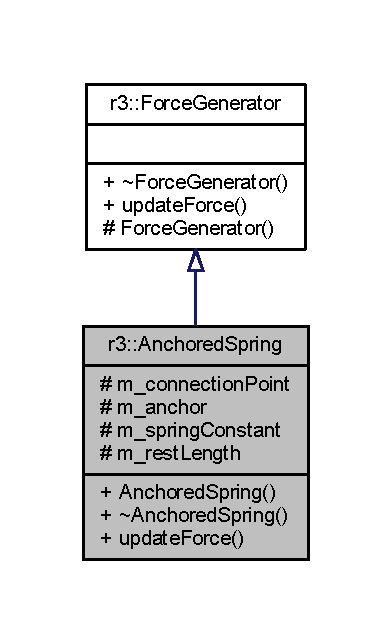
\includegraphics[width=188pt]{classr3_1_1_anchored_spring__inherit__graph}
\end{center}
\end{figure}


Collaboration diagram for r3\+:\+:Anchored\+Spring\+:\nopagebreak
\begin{figure}[H]
\begin{center}
\leavevmode
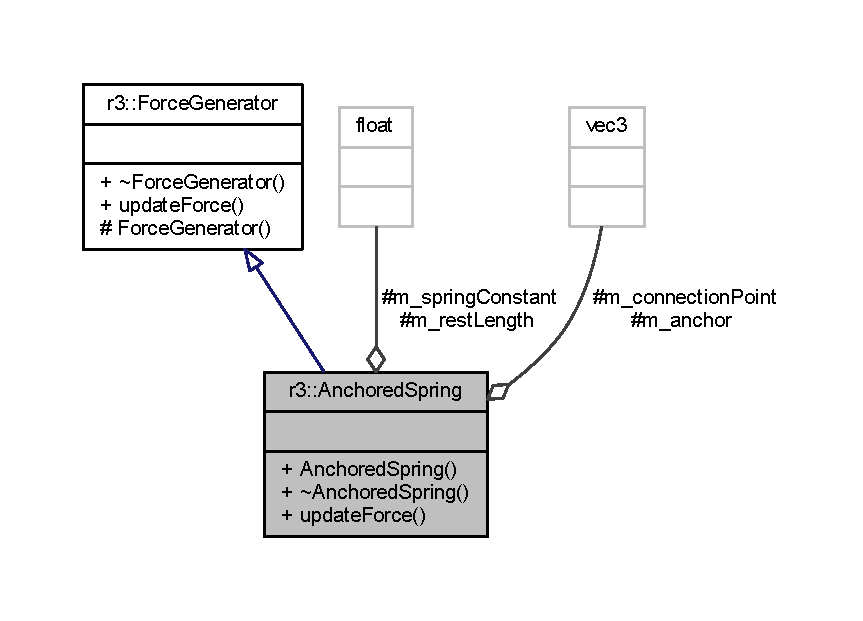
\includegraphics[width=350pt]{classr3_1_1_anchored_spring__coll__graph}
\end{center}
\end{figure}
\subsection*{Public Member Functions}
\begin{DoxyCompactItemize}
\item 
\mbox{\hyperlink{classr3_1_1_anchored_spring_a944423598dfb2e3f080f9f9850c8aa13}{Anchored\+Spring}} (const glm\+::vec3 \&anchor, const glm\+::vec3 \&local\+Connection\+Point, \mbox{\hyperlink{namespacer3_ab2016b3e3f743fb735afce242f0dc1eb}{real}} spring\+Constant, \mbox{\hyperlink{namespacer3_ab2016b3e3f743fb735afce242f0dc1eb}{real}} rest\+Length)
\item 
\mbox{\hyperlink{classr3_1_1_anchored_spring_afe612722d8ed0d7a6f0058dcc21eb17f}{$\sim$\+Anchored\+Spring}} ()
\item 
void \mbox{\hyperlink{classr3_1_1_anchored_spring_a3e928bc7fdedc8eb5b302a007200a58c}{update\+Force}} (\mbox{\hyperlink{classr3_1_1_rigid_body}{Rigid\+Body}} $\ast$body, \mbox{\hyperlink{namespacer3_ab2016b3e3f743fb735afce242f0dc1eb}{real}} duration) override
\end{DoxyCompactItemize}
\subsection*{Protected Attributes}
\begin{DoxyCompactItemize}
\item 
glm\+::vec3 \mbox{\hyperlink{classr3_1_1_anchored_spring_ac8998ca820fd075aed011136155ec1fb}{m\+\_\+connection\+Point}}
\item 
glm\+::vec3 \mbox{\hyperlink{classr3_1_1_anchored_spring_a1387aec403f6955848fe8c3a28b90a9e}{m\+\_\+anchor}}
\item 
\mbox{\hyperlink{namespacer3_ab2016b3e3f743fb735afce242f0dc1eb}{real}} \mbox{\hyperlink{classr3_1_1_anchored_spring_af17c024b5f8a025f5555946c60b52a67}{m\+\_\+spring\+Constant}}
\item 
\mbox{\hyperlink{namespacer3_ab2016b3e3f743fb735afce242f0dc1eb}{real}} \mbox{\hyperlink{classr3_1_1_anchored_spring_a17441401eb79dd8244a4739a3a574d1a}{m\+\_\+rest\+Length}}
\end{DoxyCompactItemize}
\subsection*{Additional Inherited Members}


\subsection{Constructor \& Destructor Documentation}
\mbox{\Hypertarget{classr3_1_1_anchored_spring_a944423598dfb2e3f080f9f9850c8aa13}\label{classr3_1_1_anchored_spring_a944423598dfb2e3f080f9f9850c8aa13}} 
\index{r3\+::\+Anchored\+Spring@{r3\+::\+Anchored\+Spring}!Anchored\+Spring@{Anchored\+Spring}}
\index{Anchored\+Spring@{Anchored\+Spring}!r3\+::\+Anchored\+Spring@{r3\+::\+Anchored\+Spring}}
\subsubsection{\texorpdfstring{Anchored\+Spring()}{AnchoredSpring()}}
{\footnotesize\ttfamily r3\+::\+Anchored\+Spring\+::\+Anchored\+Spring (\begin{DoxyParamCaption}\item[{const glm\+::vec3 \&}]{anchor,  }\item[{const glm\+::vec3 \&}]{local\+Connection\+Point,  }\item[{\mbox{\hyperlink{namespacer3_ab2016b3e3f743fb735afce242f0dc1eb}{real}}}]{spring\+Constant,  }\item[{\mbox{\hyperlink{namespacer3_ab2016b3e3f743fb735afce242f0dc1eb}{real}}}]{rest\+Length }\end{DoxyParamCaption})\hspace{0.3cm}{\ttfamily [explicit]}}

\mbox{\Hypertarget{classr3_1_1_anchored_spring_afe612722d8ed0d7a6f0058dcc21eb17f}\label{classr3_1_1_anchored_spring_afe612722d8ed0d7a6f0058dcc21eb17f}} 
\index{r3\+::\+Anchored\+Spring@{r3\+::\+Anchored\+Spring}!````~Anchored\+Spring@{$\sim$\+Anchored\+Spring}}
\index{````~Anchored\+Spring@{$\sim$\+Anchored\+Spring}!r3\+::\+Anchored\+Spring@{r3\+::\+Anchored\+Spring}}
\subsubsection{\texorpdfstring{$\sim$\+Anchored\+Spring()}{~AnchoredSpring()}}
{\footnotesize\ttfamily r3\+::\+Anchored\+Spring\+::$\sim$\+Anchored\+Spring (\begin{DoxyParamCaption}{ }\end{DoxyParamCaption})\hspace{0.3cm}{\ttfamily [default]}}



\subsection{Member Function Documentation}
\mbox{\Hypertarget{classr3_1_1_anchored_spring_a3e928bc7fdedc8eb5b302a007200a58c}\label{classr3_1_1_anchored_spring_a3e928bc7fdedc8eb5b302a007200a58c}} 
\index{r3\+::\+Anchored\+Spring@{r3\+::\+Anchored\+Spring}!update\+Force@{update\+Force}}
\index{update\+Force@{update\+Force}!r3\+::\+Anchored\+Spring@{r3\+::\+Anchored\+Spring}}
\subsubsection{\texorpdfstring{update\+Force()}{updateForce()}}
{\footnotesize\ttfamily void r3\+::\+Anchored\+Spring\+::update\+Force (\begin{DoxyParamCaption}\item[{\mbox{\hyperlink{classr3_1_1_rigid_body}{Rigid\+Body}} $\ast$}]{body,  }\item[{\mbox{\hyperlink{namespacer3_ab2016b3e3f743fb735afce242f0dc1eb}{real}}}]{duration }\end{DoxyParamCaption})\hspace{0.3cm}{\ttfamily [override]}, {\ttfamily [virtual]}}



Reimplemented from \mbox{\hyperlink{classr3_1_1_force_generator_a16d1e8aa85d574013de859b95944c5bb}{r3\+::\+Force\+Generator}}.



\subsection{Member Data Documentation}
\mbox{\Hypertarget{classr3_1_1_anchored_spring_a1387aec403f6955848fe8c3a28b90a9e}\label{classr3_1_1_anchored_spring_a1387aec403f6955848fe8c3a28b90a9e}} 
\index{r3\+::\+Anchored\+Spring@{r3\+::\+Anchored\+Spring}!m\+\_\+anchor@{m\+\_\+anchor}}
\index{m\+\_\+anchor@{m\+\_\+anchor}!r3\+::\+Anchored\+Spring@{r3\+::\+Anchored\+Spring}}
\subsubsection{\texorpdfstring{m\+\_\+anchor}{m\_anchor}}
{\footnotesize\ttfamily glm\+::vec3 r3\+::\+Anchored\+Spring\+::m\+\_\+anchor\hspace{0.3cm}{\ttfamily [protected]}}

\mbox{\Hypertarget{classr3_1_1_anchored_spring_ac8998ca820fd075aed011136155ec1fb}\label{classr3_1_1_anchored_spring_ac8998ca820fd075aed011136155ec1fb}} 
\index{r3\+::\+Anchored\+Spring@{r3\+::\+Anchored\+Spring}!m\+\_\+connection\+Point@{m\+\_\+connection\+Point}}
\index{m\+\_\+connection\+Point@{m\+\_\+connection\+Point}!r3\+::\+Anchored\+Spring@{r3\+::\+Anchored\+Spring}}
\subsubsection{\texorpdfstring{m\+\_\+connection\+Point}{m\_connectionPoint}}
{\footnotesize\ttfamily glm\+::vec3 r3\+::\+Anchored\+Spring\+::m\+\_\+connection\+Point\hspace{0.3cm}{\ttfamily [protected]}}

\mbox{\Hypertarget{classr3_1_1_anchored_spring_a17441401eb79dd8244a4739a3a574d1a}\label{classr3_1_1_anchored_spring_a17441401eb79dd8244a4739a3a574d1a}} 
\index{r3\+::\+Anchored\+Spring@{r3\+::\+Anchored\+Spring}!m\+\_\+rest\+Length@{m\+\_\+rest\+Length}}
\index{m\+\_\+rest\+Length@{m\+\_\+rest\+Length}!r3\+::\+Anchored\+Spring@{r3\+::\+Anchored\+Spring}}
\subsubsection{\texorpdfstring{m\+\_\+rest\+Length}{m\_restLength}}
{\footnotesize\ttfamily \mbox{\hyperlink{namespacer3_ab2016b3e3f743fb735afce242f0dc1eb}{real}} r3\+::\+Anchored\+Spring\+::m\+\_\+rest\+Length\hspace{0.3cm}{\ttfamily [protected]}}

\mbox{\Hypertarget{classr3_1_1_anchored_spring_af17c024b5f8a025f5555946c60b52a67}\label{classr3_1_1_anchored_spring_af17c024b5f8a025f5555946c60b52a67}} 
\index{r3\+::\+Anchored\+Spring@{r3\+::\+Anchored\+Spring}!m\+\_\+spring\+Constant@{m\+\_\+spring\+Constant}}
\index{m\+\_\+spring\+Constant@{m\+\_\+spring\+Constant}!r3\+::\+Anchored\+Spring@{r3\+::\+Anchored\+Spring}}
\subsubsection{\texorpdfstring{m\+\_\+spring\+Constant}{m\_springConstant}}
{\footnotesize\ttfamily \mbox{\hyperlink{namespacer3_ab2016b3e3f743fb735afce242f0dc1eb}{real}} r3\+::\+Anchored\+Spring\+::m\+\_\+spring\+Constant\hspace{0.3cm}{\ttfamily [protected]}}



The documentation for this class was generated from the following files\+:\begin{DoxyCompactItemize}
\item 
D\+:/\+Library/\+Documents/\+Job/\+Forschungsmaster/\+Projekte/\+Simulation\+Visualization/\+Rumble3\+D/\+Rumble3\+D/include/\+R3\+D/\+Rigid\+Body\+Engine/\mbox{\hyperlink{_anchored_spring_8h}{Anchored\+Spring.\+h}}\item 
D\+:/\+Library/\+Documents/\+Job/\+Forschungsmaster/\+Projekte/\+Simulation\+Visualization/\+Rumble3\+D/\+Rumble3\+D/src/\+Rigid\+Body\+Engine/\mbox{\hyperlink{_anchored_spring_8cpp}{Anchored\+Spring.\+cpp}}\end{DoxyCompactItemize}

\hypertarget{classr3_1_1_bounding_box}{}\section{r3\+:\+:Bounding\+Box Class Reference}
\label{classr3_1_1_bounding_box}\index{r3\+::\+Bounding\+Box@{r3\+::\+Bounding\+Box}}


{\ttfamily \#include $<$Bounding\+Box.\+h$>$}



Collaboration diagram for r3\+:\+:Bounding\+Box\+:\nopagebreak
\begin{figure}[H]
\begin{center}
\leavevmode
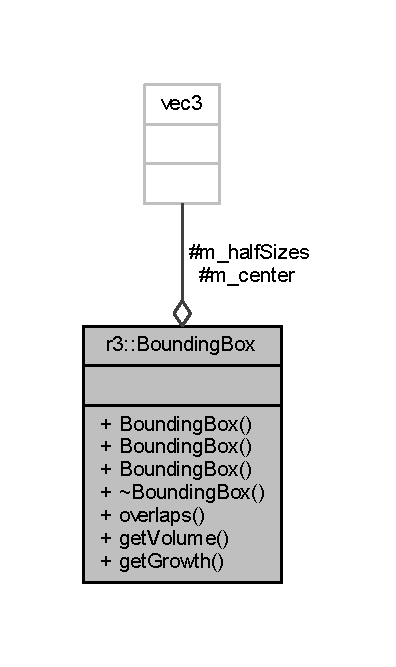
\includegraphics[width=182pt]{classr3_1_1_bounding_box__coll__graph}
\end{center}
\end{figure}
\subsection*{Public Member Functions}
\begin{DoxyCompactItemize}
\item 
\mbox{\hyperlink{classr3_1_1_bounding_box_a088852419e2b7af17f2e94d672a70bcf}{Bounding\+Box}} ()
\item 
\mbox{\hyperlink{classr3_1_1_bounding_box_abb61e82e1d736772f92b4f5b519c755d}{Bounding\+Box}} (const glm\+::vec3 \&center, const glm\+::vec3 \&bounds)
\item 
\mbox{\hyperlink{classr3_1_1_bounding_box_a23750f8e74b918e0b39ce2c2fe609574}{Bounding\+Box}} (const \mbox{\hyperlink{classr3_1_1_bounding_box}{Bounding\+Box}} \&one, const \mbox{\hyperlink{classr3_1_1_bounding_box}{Bounding\+Box}} \&two)
\item 
\mbox{\hyperlink{classr3_1_1_bounding_box_a9257cfab936d3331cba765cb19527aa1}{$\sim$\+Bounding\+Box}} ()
\item 
bool \mbox{\hyperlink{classr3_1_1_bounding_box_a6e69163febe125531fa355ae9876b8be}{overlaps}} (const \mbox{\hyperlink{classr3_1_1_bounding_box}{Bounding\+Box}} $\ast$other) const
\item 
\mbox{\hyperlink{namespacer3_ab2016b3e3f743fb735afce242f0dc1eb}{real}} \mbox{\hyperlink{classr3_1_1_bounding_box_a3e6a9b79373dde150d18d5d5df59a2f3}{get\+Volume}} () const
\item 
\mbox{\hyperlink{namespacer3_ab2016b3e3f743fb735afce242f0dc1eb}{real}} \mbox{\hyperlink{classr3_1_1_bounding_box_a21631e2fffeb995d3a9647489f936d13}{get\+Growth}} (const \mbox{\hyperlink{classr3_1_1_bounding_box}{Bounding\+Box}} \&other) const
\end{DoxyCompactItemize}
\subsection*{Protected Attributes}
\begin{DoxyCompactItemize}
\item 
glm\+::vec3 \mbox{\hyperlink{classr3_1_1_bounding_box_ae7f47ade2f27fb7e76da58c944141d80}{m\+\_\+center}}
\item 
glm\+::vec3 \mbox{\hyperlink{classr3_1_1_bounding_box_ad23e4002c102c50ac31f6bb5da6d9d39}{m\+\_\+bounds}}
\end{DoxyCompactItemize}


\subsection{Constructor \& Destructor Documentation}
\mbox{\Hypertarget{classr3_1_1_bounding_box_a088852419e2b7af17f2e94d672a70bcf}\label{classr3_1_1_bounding_box_a088852419e2b7af17f2e94d672a70bcf}} 
\index{r3\+::\+Bounding\+Box@{r3\+::\+Bounding\+Box}!Bounding\+Box@{Bounding\+Box}}
\index{Bounding\+Box@{Bounding\+Box}!r3\+::\+Bounding\+Box@{r3\+::\+Bounding\+Box}}
\subsubsection{\texorpdfstring{Bounding\+Box()}{BoundingBox()}\hspace{0.1cm}{\footnotesize\ttfamily [1/3]}}
{\footnotesize\ttfamily r3\+::\+Bounding\+Box\+::\+Bounding\+Box (\begin{DoxyParamCaption}{ }\end{DoxyParamCaption})}

\mbox{\Hypertarget{classr3_1_1_bounding_box_abb61e82e1d736772f92b4f5b519c755d}\label{classr3_1_1_bounding_box_abb61e82e1d736772f92b4f5b519c755d}} 
\index{r3\+::\+Bounding\+Box@{r3\+::\+Bounding\+Box}!Bounding\+Box@{Bounding\+Box}}
\index{Bounding\+Box@{Bounding\+Box}!r3\+::\+Bounding\+Box@{r3\+::\+Bounding\+Box}}
\subsubsection{\texorpdfstring{Bounding\+Box()}{BoundingBox()}\hspace{0.1cm}{\footnotesize\ttfamily [2/3]}}
{\footnotesize\ttfamily r3\+::\+Bounding\+Box\+::\+Bounding\+Box (\begin{DoxyParamCaption}\item[{const glm\+::vec3 \&}]{center,  }\item[{const glm\+::vec3 \&}]{bounds }\end{DoxyParamCaption})}

\mbox{\Hypertarget{classr3_1_1_bounding_box_a23750f8e74b918e0b39ce2c2fe609574}\label{classr3_1_1_bounding_box_a23750f8e74b918e0b39ce2c2fe609574}} 
\index{r3\+::\+Bounding\+Box@{r3\+::\+Bounding\+Box}!Bounding\+Box@{Bounding\+Box}}
\index{Bounding\+Box@{Bounding\+Box}!r3\+::\+Bounding\+Box@{r3\+::\+Bounding\+Box}}
\subsubsection{\texorpdfstring{Bounding\+Box()}{BoundingBox()}\hspace{0.1cm}{\footnotesize\ttfamily [3/3]}}
{\footnotesize\ttfamily r3\+::\+Bounding\+Box\+::\+Bounding\+Box (\begin{DoxyParamCaption}\item[{const \mbox{\hyperlink{classr3_1_1_bounding_box}{Bounding\+Box}} \&}]{one,  }\item[{const \mbox{\hyperlink{classr3_1_1_bounding_box}{Bounding\+Box}} \&}]{two }\end{DoxyParamCaption})}

\mbox{\Hypertarget{classr3_1_1_bounding_box_a9257cfab936d3331cba765cb19527aa1}\label{classr3_1_1_bounding_box_a9257cfab936d3331cba765cb19527aa1}} 
\index{r3\+::\+Bounding\+Box@{r3\+::\+Bounding\+Box}!````~Bounding\+Box@{$\sim$\+Bounding\+Box}}
\index{````~Bounding\+Box@{$\sim$\+Bounding\+Box}!r3\+::\+Bounding\+Box@{r3\+::\+Bounding\+Box}}
\subsubsection{\texorpdfstring{$\sim$\+Bounding\+Box()}{~BoundingBox()}}
{\footnotesize\ttfamily r3\+::\+Bounding\+Box\+::$\sim$\+Bounding\+Box (\begin{DoxyParamCaption}{ }\end{DoxyParamCaption})}



\subsection{Member Function Documentation}
\mbox{\Hypertarget{classr3_1_1_bounding_box_a21631e2fffeb995d3a9647489f936d13}\label{classr3_1_1_bounding_box_a21631e2fffeb995d3a9647489f936d13}} 
\index{r3\+::\+Bounding\+Box@{r3\+::\+Bounding\+Box}!get\+Growth@{get\+Growth}}
\index{get\+Growth@{get\+Growth}!r3\+::\+Bounding\+Box@{r3\+::\+Bounding\+Box}}
\subsubsection{\texorpdfstring{get\+Growth()}{getGrowth()}}
{\footnotesize\ttfamily \mbox{\hyperlink{namespacer3_ab2016b3e3f743fb735afce242f0dc1eb}{real}} r3\+::\+Bounding\+Box\+::get\+Growth (\begin{DoxyParamCaption}\item[{const \mbox{\hyperlink{classr3_1_1_bounding_box}{Bounding\+Box}} \&}]{other }\end{DoxyParamCaption}) const}

\mbox{\Hypertarget{classr3_1_1_bounding_box_a3e6a9b79373dde150d18d5d5df59a2f3}\label{classr3_1_1_bounding_box_a3e6a9b79373dde150d18d5d5df59a2f3}} 
\index{r3\+::\+Bounding\+Box@{r3\+::\+Bounding\+Box}!get\+Volume@{get\+Volume}}
\index{get\+Volume@{get\+Volume}!r3\+::\+Bounding\+Box@{r3\+::\+Bounding\+Box}}
\subsubsection{\texorpdfstring{get\+Volume()}{getVolume()}}
{\footnotesize\ttfamily \mbox{\hyperlink{namespacer3_ab2016b3e3f743fb735afce242f0dc1eb}{real}} r3\+::\+Bounding\+Box\+::get\+Volume (\begin{DoxyParamCaption}{ }\end{DoxyParamCaption}) const}

Get the volume of this bounding box. \mbox{\Hypertarget{classr3_1_1_bounding_box_a6e69163febe125531fa355ae9876b8be}\label{classr3_1_1_bounding_box_a6e69163febe125531fa355ae9876b8be}} 
\index{r3\+::\+Bounding\+Box@{r3\+::\+Bounding\+Box}!overlaps@{overlaps}}
\index{overlaps@{overlaps}!r3\+::\+Bounding\+Box@{r3\+::\+Bounding\+Box}}
\subsubsection{\texorpdfstring{overlaps()}{overlaps()}}
{\footnotesize\ttfamily bool r3\+::\+Bounding\+Box\+::overlaps (\begin{DoxyParamCaption}\item[{const \mbox{\hyperlink{classr3_1_1_bounding_box}{Bounding\+Box}} $\ast$}]{other }\end{DoxyParamCaption}) const}



\subsection{Member Data Documentation}
\mbox{\Hypertarget{classr3_1_1_bounding_box_ad23e4002c102c50ac31f6bb5da6d9d39}\label{classr3_1_1_bounding_box_ad23e4002c102c50ac31f6bb5da6d9d39}} 
\index{r3\+::\+Bounding\+Box@{r3\+::\+Bounding\+Box}!m\+\_\+bounds@{m\+\_\+bounds}}
\index{m\+\_\+bounds@{m\+\_\+bounds}!r3\+::\+Bounding\+Box@{r3\+::\+Bounding\+Box}}
\subsubsection{\texorpdfstring{m\+\_\+bounds}{m\_bounds}}
{\footnotesize\ttfamily glm\+::vec3 r3\+::\+Bounding\+Box\+::m\+\_\+bounds\hspace{0.3cm}{\ttfamily [protected]}}

\mbox{\Hypertarget{classr3_1_1_bounding_box_ae7f47ade2f27fb7e76da58c944141d80}\label{classr3_1_1_bounding_box_ae7f47ade2f27fb7e76da58c944141d80}} 
\index{r3\+::\+Bounding\+Box@{r3\+::\+Bounding\+Box}!m\+\_\+center@{m\+\_\+center}}
\index{m\+\_\+center@{m\+\_\+center}!r3\+::\+Bounding\+Box@{r3\+::\+Bounding\+Box}}
\subsubsection{\texorpdfstring{m\+\_\+center}{m\_center}}
{\footnotesize\ttfamily glm\+::vec3 r3\+::\+Bounding\+Box\+::m\+\_\+center\hspace{0.3cm}{\ttfamily [protected]}}



The documentation for this class was generated from the following files\+:\begin{DoxyCompactItemize}
\item 
D\+:/\+Job/\+Forschungsmaster/\+Projekte/\+Simulation\+Visualization/\+Rumble3\+D/\+Rumble3\+D/include/\+R3\+D/\+Rigid\+Body\+Engine/\mbox{\hyperlink{_bounding_box_8h}{Bounding\+Box.\+h}}\item 
D\+:/\+Job/\+Forschungsmaster/\+Projekte/\+Simulation\+Visualization/\+Rumble3\+D/\+Rumble3\+D/src/\+Rigid\+Body\+Engine/\mbox{\hyperlink{_bounding_box_8cpp}{Bounding\+Box.\+cpp}}\end{DoxyCompactItemize}

\hypertarget{classr3_1_1_bounding_sphere}{}\section{r3\+:\+:Bounding\+Sphere Class Reference}
\label{classr3_1_1_bounding_sphere}\index{r3\+::\+Bounding\+Sphere@{r3\+::\+Bounding\+Sphere}}


A bounding sphere is a kind of bounding volume.  




{\ttfamily \#include $<$Bounding\+Sphere.\+h$>$}



Collaboration diagram for r3\+:\+:Bounding\+Sphere\+:\nopagebreak
\begin{figure}[H]
\begin{center}
\leavevmode
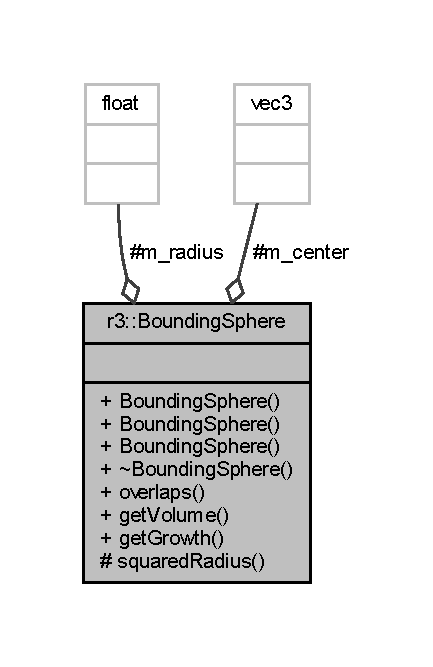
\includegraphics[width=208pt]{classr3_1_1_bounding_sphere__coll__graph}
\end{center}
\end{figure}
\subsection*{Public Member Functions}
\begin{DoxyCompactItemize}
\item 
\mbox{\hyperlink{classr3_1_1_bounding_sphere_af602a853d8ed0b5ccad8679ee41fe7f8}{Bounding\+Sphere}} ()
\item 
\mbox{\hyperlink{classr3_1_1_bounding_sphere_a9a9264c19d56b10c9b0def547a369d57}{Bounding\+Sphere}} (const glm\+::vec3 \&center, \mbox{\hyperlink{namespacer3_ab2016b3e3f743fb735afce242f0dc1eb}{real}} radius)
\begin{DoxyCompactList}\small\item\em \mbox{\hyperlink{classr3_1_1_bounding_box}{Bounding\+Box}} constructor. \end{DoxyCompactList}\item 
\mbox{\hyperlink{classr3_1_1_bounding_sphere_a3d461e62b827ad9a30ca8013d451e3da}{Bounding\+Sphere}} (const \mbox{\hyperlink{classr3_1_1_bounding_sphere}{Bounding\+Sphere}} \&one, const \mbox{\hyperlink{classr3_1_1_bounding_sphere}{Bounding\+Sphere}} \&two)
\begin{DoxyCompactList}\small\item\em \mbox{\hyperlink{classr3_1_1_bounding_sphere}{Bounding\+Sphere}} constructor. \end{DoxyCompactList}\item 
\mbox{\hyperlink{classr3_1_1_bounding_sphere_a9951f8922ebb2227cd97e59c97fed2a5}{$\sim$\+Bounding\+Sphere}} ()
\item 
bool \mbox{\hyperlink{classr3_1_1_bounding_sphere_a49163c78b0d1318c576d99e61f806ac2}{overlaps}} (const \mbox{\hyperlink{classr3_1_1_bounding_sphere}{Bounding\+Sphere}} $\ast$other) const
\begin{DoxyCompactList}\small\item\em Check if this bounding sphere overlaps with the given bounding sphere. \end{DoxyCompactList}\item 
\mbox{\hyperlink{namespacer3_ab2016b3e3f743fb735afce242f0dc1eb}{real}} \mbox{\hyperlink{classr3_1_1_bounding_sphere_a01cc1a7397eeec86d2b074d2bf734798}{get\+Volume}} () const
\item 
\mbox{\hyperlink{namespacer3_ab2016b3e3f743fb735afce242f0dc1eb}{real}} \mbox{\hyperlink{classr3_1_1_bounding_sphere_ac13a86be56c1c52b33a707eb2356daa3}{get\+Growth}} (const \mbox{\hyperlink{classr3_1_1_bounding_sphere}{Bounding\+Sphere}} \&other) const
\begin{DoxyCompactList}\small\item\em Get an approximation of how much a new bounding sphere, including the given and this one, would be relatively to this one. \end{DoxyCompactList}\end{DoxyCompactItemize}
\subsection*{Protected Member Functions}
\begin{DoxyCompactItemize}
\item 
\mbox{\hyperlink{namespacer3_ab2016b3e3f743fb735afce242f0dc1eb}{real}} \mbox{\hyperlink{classr3_1_1_bounding_sphere_ae0e7a71b8cfe2f3287397ac865545ee4}{squared\+Radius}} () const
\begin{DoxyCompactList}\small\item\em Calculate the square of this spheres radius. \end{DoxyCompactList}\end{DoxyCompactItemize}
\subsection*{Protected Attributes}
\begin{DoxyCompactItemize}
\item 
glm\+::vec3 \mbox{\hyperlink{classr3_1_1_bounding_sphere_a880d9888f25b016c5c38c608e16fa61e}{m\+\_\+center}}
\item 
\mbox{\hyperlink{namespacer3_ab2016b3e3f743fb735afce242f0dc1eb}{real}} \mbox{\hyperlink{classr3_1_1_bounding_sphere_a37ccefd38d8cea7a0d52b85f771ec7c4}{m\+\_\+radius}} \{\}
\end{DoxyCompactItemize}


\subsection{Detailed Description}
A bounding sphere is a kind of bounding volume. 

\subsection{Constructor \& Destructor Documentation}
\mbox{\Hypertarget{classr3_1_1_bounding_sphere_af602a853d8ed0b5ccad8679ee41fe7f8}\label{classr3_1_1_bounding_sphere_af602a853d8ed0b5ccad8679ee41fe7f8}} 
\index{r3\+::\+Bounding\+Sphere@{r3\+::\+Bounding\+Sphere}!Bounding\+Sphere@{Bounding\+Sphere}}
\index{Bounding\+Sphere@{Bounding\+Sphere}!r3\+::\+Bounding\+Sphere@{r3\+::\+Bounding\+Sphere}}
\subsubsection{\texorpdfstring{Bounding\+Sphere()}{BoundingSphere()}\hspace{0.1cm}{\footnotesize\ttfamily [1/3]}}
{\footnotesize\ttfamily r3\+::\+Bounding\+Sphere\+::\+Bounding\+Sphere (\begin{DoxyParamCaption}{ }\end{DoxyParamCaption})\hspace{0.3cm}{\ttfamily [default]}}

\mbox{\Hypertarget{classr3_1_1_bounding_sphere_a9a9264c19d56b10c9b0def547a369d57}\label{classr3_1_1_bounding_sphere_a9a9264c19d56b10c9b0def547a369d57}} 
\index{r3\+::\+Bounding\+Sphere@{r3\+::\+Bounding\+Sphere}!Bounding\+Sphere@{Bounding\+Sphere}}
\index{Bounding\+Sphere@{Bounding\+Sphere}!r3\+::\+Bounding\+Sphere@{r3\+::\+Bounding\+Sphere}}
\subsubsection{\texorpdfstring{Bounding\+Sphere()}{BoundingSphere()}\hspace{0.1cm}{\footnotesize\ttfamily [2/3]}}
{\footnotesize\ttfamily r3\+::\+Bounding\+Sphere\+::\+Bounding\+Sphere (\begin{DoxyParamCaption}\item[{const glm\+::vec3 \&}]{center,  }\item[{\mbox{\hyperlink{namespacer3_ab2016b3e3f743fb735afce242f0dc1eb}{real}}}]{radius }\end{DoxyParamCaption})}



\mbox{\hyperlink{classr3_1_1_bounding_box}{Bounding\+Box}} constructor. 


\begin{DoxyParams}{Parameters}
{\em center} & The center of the spehere in world coordinates. \\
\hline
{\em radius} & The radius of the sphere \\
\hline
\end{DoxyParams}
\mbox{\Hypertarget{classr3_1_1_bounding_sphere_a3d461e62b827ad9a30ca8013d451e3da}\label{classr3_1_1_bounding_sphere_a3d461e62b827ad9a30ca8013d451e3da}} 
\index{r3\+::\+Bounding\+Sphere@{r3\+::\+Bounding\+Sphere}!Bounding\+Sphere@{Bounding\+Sphere}}
\index{Bounding\+Sphere@{Bounding\+Sphere}!r3\+::\+Bounding\+Sphere@{r3\+::\+Bounding\+Sphere}}
\subsubsection{\texorpdfstring{Bounding\+Sphere()}{BoundingSphere()}\hspace{0.1cm}{\footnotesize\ttfamily [3/3]}}
{\footnotesize\ttfamily r3\+::\+Bounding\+Sphere\+::\+Bounding\+Sphere (\begin{DoxyParamCaption}\item[{const \mbox{\hyperlink{classr3_1_1_bounding_sphere}{Bounding\+Sphere}} \&}]{one,  }\item[{const \mbox{\hyperlink{classr3_1_1_bounding_sphere}{Bounding\+Sphere}} \&}]{two }\end{DoxyParamCaption})}



\mbox{\hyperlink{classr3_1_1_bounding_sphere}{Bounding\+Sphere}} constructor. 

Create a bounding sphere which contains both given spheres. ~\newline

\begin{DoxyParams}{Parameters}
{\em one} & The first child bounding sphere. \\
\hline
{\em two} & The second child bounding sphere. \\
\hline
\end{DoxyParams}
\mbox{\Hypertarget{classr3_1_1_bounding_sphere_a9951f8922ebb2227cd97e59c97fed2a5}\label{classr3_1_1_bounding_sphere_a9951f8922ebb2227cd97e59c97fed2a5}} 
\index{r3\+::\+Bounding\+Sphere@{r3\+::\+Bounding\+Sphere}!````~Bounding\+Sphere@{$\sim$\+Bounding\+Sphere}}
\index{````~Bounding\+Sphere@{$\sim$\+Bounding\+Sphere}!r3\+::\+Bounding\+Sphere@{r3\+::\+Bounding\+Sphere}}
\subsubsection{\texorpdfstring{$\sim$\+Bounding\+Sphere()}{~BoundingSphere()}}
{\footnotesize\ttfamily r3\+::\+Bounding\+Sphere\+::$\sim$\+Bounding\+Sphere (\begin{DoxyParamCaption}{ }\end{DoxyParamCaption})\hspace{0.3cm}{\ttfamily [default]}}



\subsection{Member Function Documentation}
\mbox{\Hypertarget{classr3_1_1_bounding_sphere_ac13a86be56c1c52b33a707eb2356daa3}\label{classr3_1_1_bounding_sphere_ac13a86be56c1c52b33a707eb2356daa3}} 
\index{r3\+::\+Bounding\+Sphere@{r3\+::\+Bounding\+Sphere}!get\+Growth@{get\+Growth}}
\index{get\+Growth@{get\+Growth}!r3\+::\+Bounding\+Sphere@{r3\+::\+Bounding\+Sphere}}
\subsubsection{\texorpdfstring{get\+Growth()}{getGrowth()}}
{\footnotesize\ttfamily \mbox{\hyperlink{namespacer3_ab2016b3e3f743fb735afce242f0dc1eb}{real}} r3\+::\+Bounding\+Sphere\+::get\+Growth (\begin{DoxyParamCaption}\item[{const \mbox{\hyperlink{classr3_1_1_bounding_sphere}{Bounding\+Sphere}} \&}]{other }\end{DoxyParamCaption}) const}



Get an approximation of how much a new bounding sphere, including the given and this one, would be relatively to this one. 


\begin{DoxyParams}{Parameters}
{\em other} & The added volume. \\
\hline
\end{DoxyParams}
\begin{DoxyReturn}{Returns}
The growth. 
\end{DoxyReturn}
\mbox{\Hypertarget{classr3_1_1_bounding_sphere_a01cc1a7397eeec86d2b074d2bf734798}\label{classr3_1_1_bounding_sphere_a01cc1a7397eeec86d2b074d2bf734798}} 
\index{r3\+::\+Bounding\+Sphere@{r3\+::\+Bounding\+Sphere}!get\+Volume@{get\+Volume}}
\index{get\+Volume@{get\+Volume}!r3\+::\+Bounding\+Sphere@{r3\+::\+Bounding\+Sphere}}
\subsubsection{\texorpdfstring{get\+Volume()}{getVolume()}}
{\footnotesize\ttfamily \mbox{\hyperlink{namespacer3_ab2016b3e3f743fb735afce242f0dc1eb}{real}} r3\+::\+Bounding\+Sphere\+::get\+Volume (\begin{DoxyParamCaption}{ }\end{DoxyParamCaption}) const}

Get the volume of this bounding sphere. \begin{DoxyReturn}{Returns}
The volume. 
\end{DoxyReturn}
\mbox{\Hypertarget{classr3_1_1_bounding_sphere_a49163c78b0d1318c576d99e61f806ac2}\label{classr3_1_1_bounding_sphere_a49163c78b0d1318c576d99e61f806ac2}} 
\index{r3\+::\+Bounding\+Sphere@{r3\+::\+Bounding\+Sphere}!overlaps@{overlaps}}
\index{overlaps@{overlaps}!r3\+::\+Bounding\+Sphere@{r3\+::\+Bounding\+Sphere}}
\subsubsection{\texorpdfstring{overlaps()}{overlaps()}}
{\footnotesize\ttfamily bool r3\+::\+Bounding\+Sphere\+::overlaps (\begin{DoxyParamCaption}\item[{const \mbox{\hyperlink{classr3_1_1_bounding_sphere}{Bounding\+Sphere}} $\ast$}]{other }\end{DoxyParamCaption}) const}



Check if this bounding sphere overlaps with the given bounding sphere. 

\begin{DoxyReturn}{Returns}
True if they overlap, false otherwise. 
\end{DoxyReturn}
\mbox{\Hypertarget{classr3_1_1_bounding_sphere_ae0e7a71b8cfe2f3287397ac865545ee4}\label{classr3_1_1_bounding_sphere_ae0e7a71b8cfe2f3287397ac865545ee4}} 
\index{r3\+::\+Bounding\+Sphere@{r3\+::\+Bounding\+Sphere}!squared\+Radius@{squared\+Radius}}
\index{squared\+Radius@{squared\+Radius}!r3\+::\+Bounding\+Sphere@{r3\+::\+Bounding\+Sphere}}
\subsubsection{\texorpdfstring{squared\+Radius()}{squaredRadius()}}
{\footnotesize\ttfamily \mbox{\hyperlink{namespacer3_ab2016b3e3f743fb735afce242f0dc1eb}{real}} r3\+::\+Bounding\+Sphere\+::squared\+Radius (\begin{DoxyParamCaption}{ }\end{DoxyParamCaption}) const\hspace{0.3cm}{\ttfamily [protected]}}



Calculate the square of this spheres radius. 

\begin{DoxyReturn}{Returns}
The squared radius. 
\end{DoxyReturn}


\subsection{Member Data Documentation}
\mbox{\Hypertarget{classr3_1_1_bounding_sphere_a880d9888f25b016c5c38c608e16fa61e}\label{classr3_1_1_bounding_sphere_a880d9888f25b016c5c38c608e16fa61e}} 
\index{r3\+::\+Bounding\+Sphere@{r3\+::\+Bounding\+Sphere}!m\+\_\+center@{m\+\_\+center}}
\index{m\+\_\+center@{m\+\_\+center}!r3\+::\+Bounding\+Sphere@{r3\+::\+Bounding\+Sphere}}
\subsubsection{\texorpdfstring{m\+\_\+center}{m\_center}}
{\footnotesize\ttfamily glm\+::vec3 r3\+::\+Bounding\+Sphere\+::m\+\_\+center\hspace{0.3cm}{\ttfamily [protected]}}

\mbox{\Hypertarget{classr3_1_1_bounding_sphere_a37ccefd38d8cea7a0d52b85f771ec7c4}\label{classr3_1_1_bounding_sphere_a37ccefd38d8cea7a0d52b85f771ec7c4}} 
\index{r3\+::\+Bounding\+Sphere@{r3\+::\+Bounding\+Sphere}!m\+\_\+radius@{m\+\_\+radius}}
\index{m\+\_\+radius@{m\+\_\+radius}!r3\+::\+Bounding\+Sphere@{r3\+::\+Bounding\+Sphere}}
\subsubsection{\texorpdfstring{m\+\_\+radius}{m\_radius}}
{\footnotesize\ttfamily \mbox{\hyperlink{namespacer3_ab2016b3e3f743fb735afce242f0dc1eb}{real}} r3\+::\+Bounding\+Sphere\+::m\+\_\+radius \{\}\hspace{0.3cm}{\ttfamily [protected]}}



The documentation for this class was generated from the following files\+:\begin{DoxyCompactItemize}
\item 
C\+:/\+Library/\+Job/\+Projekte/\+Simulation\+Visualization/\+Rumble3\+D/\+Rumble3\+D/include/\+R3\+D/\+Rigid\+Body\+Engine/\mbox{\hyperlink{_bounding_sphere_8h}{Bounding\+Sphere.\+h}}\item 
C\+:/\+Library/\+Job/\+Projekte/\+Simulation\+Visualization/\+Rumble3\+D/\+Rumble3\+D/src/\+Rigid\+Body\+Engine/\mbox{\hyperlink{_bounding_sphere_8cpp}{Bounding\+Sphere.\+cpp}}\end{DoxyCompactItemize}

\hypertarget{classr3_1_1_box_box_narrow_algorithm}{}\section{r3\+:\+:Box\+Box\+Narrow\+Algorithm Class Reference}
\label{classr3_1_1_box_box_narrow_algorithm}\index{r3\+::\+Box\+Box\+Narrow\+Algorithm@{r3\+::\+Box\+Box\+Narrow\+Algorithm}}


Default implementation for a box-\/box narrow algorithm.  




{\ttfamily \#include $<$Box\+Box\+Narrow\+Algorithm.\+h$>$}



Inheritance diagram for r3\+:\+:Box\+Box\+Narrow\+Algorithm\+:\nopagebreak
\begin{figure}[H]
\begin{center}
\leavevmode
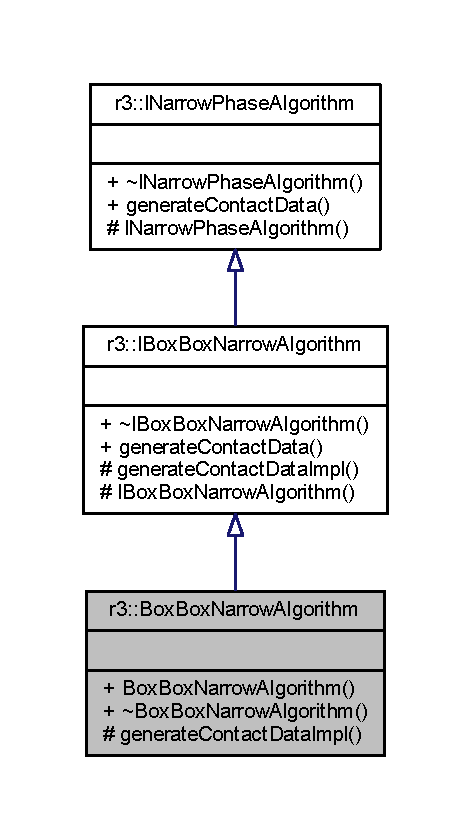
\includegraphics[width=226pt]{classr3_1_1_box_box_narrow_algorithm__inherit__graph}
\end{center}
\end{figure}


Collaboration diagram for r3\+:\+:Box\+Box\+Narrow\+Algorithm\+:\nopagebreak
\begin{figure}[H]
\begin{center}
\leavevmode
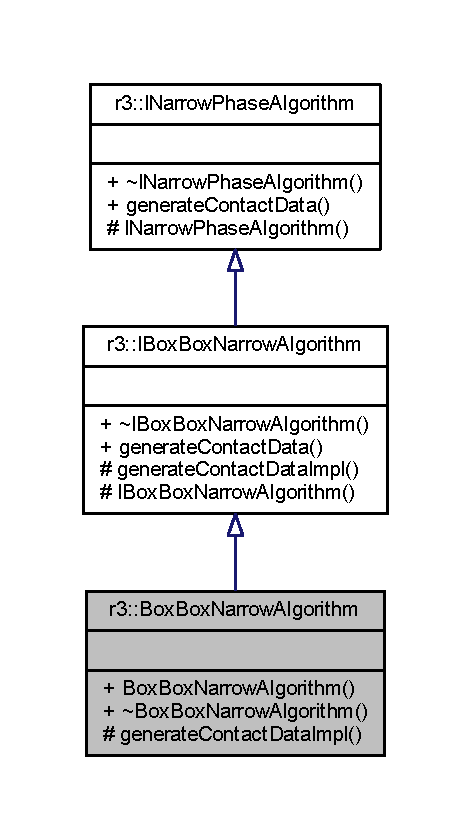
\includegraphics[width=226pt]{classr3_1_1_box_box_narrow_algorithm__coll__graph}
\end{center}
\end{figure}
\subsection*{Public Member Functions}
\begin{DoxyCompactItemize}
\item 
\mbox{\hyperlink{classr3_1_1_box_box_narrow_algorithm_a3c801622b4235a4738d18fef0eda9949}{Box\+Box\+Narrow\+Algorithm}} ()
\item 
\mbox{\hyperlink{classr3_1_1_box_box_narrow_algorithm_a67eb8bd09d7531a5917ac5e720733075}{$\sim$\+Box\+Box\+Narrow\+Algorithm}} ()
\end{DoxyCompactItemize}
\subsection*{Protected Member Functions}
\begin{DoxyCompactItemize}
\item 
bool \mbox{\hyperlink{classr3_1_1_box_box_narrow_algorithm_a200098ad4e6e2381f58856002a2d5dec}{generate\+Contact\+Data\+Impl}} (\mbox{\hyperlink{classr3_1_1_rigid_body}{Rigid\+Body}} $\ast$rb\+Box1, \mbox{\hyperlink{classr3_1_1_collision_box}{Collision\+Box}} $\ast$box1, \mbox{\hyperlink{classr3_1_1_rigid_body}{Rigid\+Body}} $\ast$rb\+Box2, \mbox{\hyperlink{classr3_1_1_collision_box}{Collision\+Box}} $\ast$box2, \mbox{\hyperlink{classr3_1_1_collision_data}{Collision\+Data}} \&collision\+Data) override
\end{DoxyCompactItemize}


\subsection{Detailed Description}
Default implementation for a box-\/box narrow algorithm. 

\subsection{Constructor \& Destructor Documentation}
\mbox{\Hypertarget{classr3_1_1_box_box_narrow_algorithm_a3c801622b4235a4738d18fef0eda9949}\label{classr3_1_1_box_box_narrow_algorithm_a3c801622b4235a4738d18fef0eda9949}} 
\index{r3\+::\+Box\+Box\+Narrow\+Algorithm@{r3\+::\+Box\+Box\+Narrow\+Algorithm}!Box\+Box\+Narrow\+Algorithm@{Box\+Box\+Narrow\+Algorithm}}
\index{Box\+Box\+Narrow\+Algorithm@{Box\+Box\+Narrow\+Algorithm}!r3\+::\+Box\+Box\+Narrow\+Algorithm@{r3\+::\+Box\+Box\+Narrow\+Algorithm}}
\subsubsection{\texorpdfstring{Box\+Box\+Narrow\+Algorithm()}{BoxBoxNarrowAlgorithm()}}
{\footnotesize\ttfamily r3\+::\+Box\+Box\+Narrow\+Algorithm\+::\+Box\+Box\+Narrow\+Algorithm (\begin{DoxyParamCaption}{ }\end{DoxyParamCaption})\hspace{0.3cm}{\ttfamily [explicit]}, {\ttfamily [default]}}

\mbox{\Hypertarget{classr3_1_1_box_box_narrow_algorithm_a67eb8bd09d7531a5917ac5e720733075}\label{classr3_1_1_box_box_narrow_algorithm_a67eb8bd09d7531a5917ac5e720733075}} 
\index{r3\+::\+Box\+Box\+Narrow\+Algorithm@{r3\+::\+Box\+Box\+Narrow\+Algorithm}!````~Box\+Box\+Narrow\+Algorithm@{$\sim$\+Box\+Box\+Narrow\+Algorithm}}
\index{````~Box\+Box\+Narrow\+Algorithm@{$\sim$\+Box\+Box\+Narrow\+Algorithm}!r3\+::\+Box\+Box\+Narrow\+Algorithm@{r3\+::\+Box\+Box\+Narrow\+Algorithm}}
\subsubsection{\texorpdfstring{$\sim$\+Box\+Box\+Narrow\+Algorithm()}{~BoxBoxNarrowAlgorithm()}}
{\footnotesize\ttfamily r3\+::\+Box\+Box\+Narrow\+Algorithm\+::$\sim$\+Box\+Box\+Narrow\+Algorithm (\begin{DoxyParamCaption}{ }\end{DoxyParamCaption})\hspace{0.3cm}{\ttfamily [default]}}



\subsection{Member Function Documentation}
\mbox{\Hypertarget{classr3_1_1_box_box_narrow_algorithm_a200098ad4e6e2381f58856002a2d5dec}\label{classr3_1_1_box_box_narrow_algorithm_a200098ad4e6e2381f58856002a2d5dec}} 
\index{r3\+::\+Box\+Box\+Narrow\+Algorithm@{r3\+::\+Box\+Box\+Narrow\+Algorithm}!generate\+Contact\+Data\+Impl@{generate\+Contact\+Data\+Impl}}
\index{generate\+Contact\+Data\+Impl@{generate\+Contact\+Data\+Impl}!r3\+::\+Box\+Box\+Narrow\+Algorithm@{r3\+::\+Box\+Box\+Narrow\+Algorithm}}
\subsubsection{\texorpdfstring{generate\+Contact\+Data\+Impl()}{generateContactDataImpl()}}
{\footnotesize\ttfamily bool r3\+::\+Box\+Box\+Narrow\+Algorithm\+::generate\+Contact\+Data\+Impl (\begin{DoxyParamCaption}\item[{\mbox{\hyperlink{classr3_1_1_rigid_body}{Rigid\+Body}} $\ast$}]{rb\+Box1,  }\item[{\mbox{\hyperlink{classr3_1_1_collision_box}{Collision\+Box}} $\ast$}]{box1,  }\item[{\mbox{\hyperlink{classr3_1_1_rigid_body}{Rigid\+Body}} $\ast$}]{rb\+Box2,  }\item[{\mbox{\hyperlink{classr3_1_1_collision_box}{Collision\+Box}} $\ast$}]{box2,  }\item[{\mbox{\hyperlink{classr3_1_1_collision_data}{Collision\+Data}} \&}]{collision\+Data }\end{DoxyParamCaption})\hspace{0.3cm}{\ttfamily [override]}, {\ttfamily [protected]}, {\ttfamily [virtual]}}

\begin{DoxyRefDesc}{Todo}
\item[\mbox{\hyperlink{todo__todo000013}{Todo}}]variable is never set??? \end{DoxyRefDesc}


\begin{DoxyRefDesc}{Todo}
\item[\mbox{\hyperlink{todo__todo000014}{Todo}}]\+: crash -\/$>$ best stays 0xffffff \end{DoxyRefDesc}


Implements \mbox{\hyperlink{classr3_1_1_i_box_box_narrow_algorithm_abc15898100b5ed0537e4c6ccc6610069}{r3\+::\+I\+Box\+Box\+Narrow\+Algorithm}}.



The documentation for this class was generated from the following files\+:\begin{DoxyCompactItemize}
\item 
C\+:/\+Library/\+Job/\+Projekte/\+Simulation\+Visualization/\+Rumble3\+D/\+Rumble3\+D/include/\+R3\+D/\+Rigid\+Body\+Engine/\+Collision\+Detection/\+Algorithm/\mbox{\hyperlink{_box_box_narrow_algorithm_8h}{Box\+Box\+Narrow\+Algorithm.\+h}}\item 
C\+:/\+Library/\+Job/\+Projekte/\+Simulation\+Visualization/\+Rumble3\+D/\+Rumble3\+D/src/\+Rigid\+Body\+Engine/\+Collision\+Detection/\+Algorithm/\mbox{\hyperlink{_box_box_narrow_algorithm_8cpp}{Box\+Box\+Narrow\+Algorithm.\+cpp}}\end{DoxyCompactItemize}

\hypertarget{classr3_1_1_box_sphere_narrow_algorithm}{}\section{r3\+:\+:Box\+Sphere\+Narrow\+Algorithm Class Reference}
\label{classr3_1_1_box_sphere_narrow_algorithm}\index{r3\+::\+Box\+Sphere\+Narrow\+Algorithm@{r3\+::\+Box\+Sphere\+Narrow\+Algorithm}}


Default implementation for a box-\/sphere narrow algorithm.  




{\ttfamily \#include $<$Box\+Sphere\+Narrow\+Algorithm.\+h$>$}



Inheritance diagram for r3\+:\+:Box\+Sphere\+Narrow\+Algorithm\+:\nopagebreak
\begin{figure}[H]
\begin{center}
\leavevmode
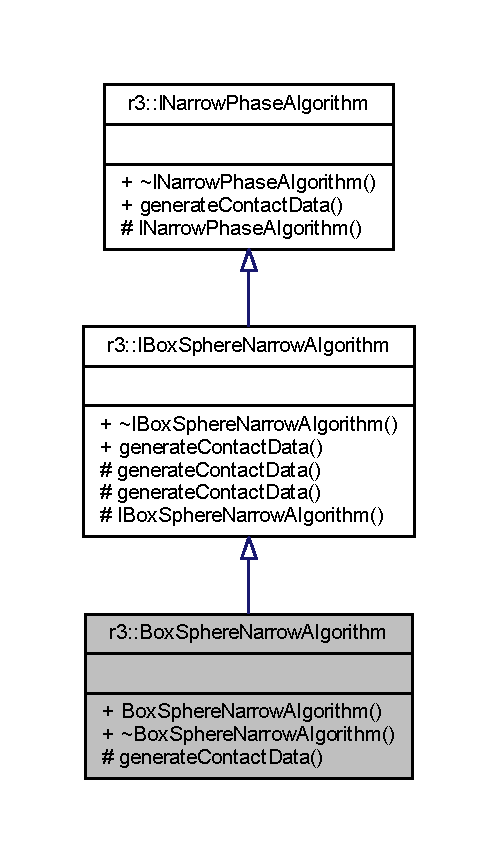
\includegraphics[width=239pt]{classr3_1_1_box_sphere_narrow_algorithm__inherit__graph}
\end{center}
\end{figure}


Collaboration diagram for r3\+:\+:Box\+Sphere\+Narrow\+Algorithm\+:\nopagebreak
\begin{figure}[H]
\begin{center}
\leavevmode
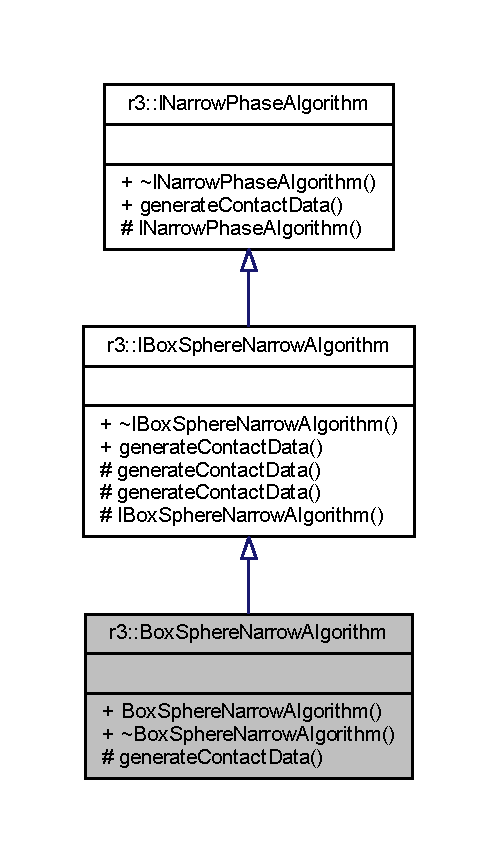
\includegraphics[width=239pt]{classr3_1_1_box_sphere_narrow_algorithm__coll__graph}
\end{center}
\end{figure}
\subsection*{Public Member Functions}
\begin{DoxyCompactItemize}
\item 
\mbox{\hyperlink{classr3_1_1_box_sphere_narrow_algorithm_a0184c33ce7da891240781ad7c78bd9a2}{Box\+Sphere\+Narrow\+Algorithm}} ()
\item 
\mbox{\hyperlink{classr3_1_1_box_sphere_narrow_algorithm_ab00e17b38da83e9a159aa7786a7a1f95}{$\sim$\+Box\+Sphere\+Narrow\+Algorithm}} ()
\end{DoxyCompactItemize}
\subsection*{Protected Member Functions}
\begin{DoxyCompactItemize}
\item 
bool \mbox{\hyperlink{classr3_1_1_box_sphere_narrow_algorithm_a2fc345fdec27e85f0e569afa0d500865}{generate\+Contact\+Data\+Impl}} (\mbox{\hyperlink{classr3_1_1_rigid_body}{Rigid\+Body}} $\ast$rb\+Box, \mbox{\hyperlink{classr3_1_1_collision_box}{Collision\+Box}} $\ast$box, \mbox{\hyperlink{classr3_1_1_rigid_body}{Rigid\+Body}} $\ast$rb\+Sphere, \mbox{\hyperlink{classr3_1_1_collision_sphere}{Collision\+Sphere}} $\ast$sphere, \mbox{\hyperlink{classr3_1_1_collision_data}{Collision\+Data}} \&collision\+Data) override
\end{DoxyCompactItemize}


\subsection{Detailed Description}
Default implementation for a box-\/sphere narrow algorithm. 

\subsection{Constructor \& Destructor Documentation}
\mbox{\Hypertarget{classr3_1_1_box_sphere_narrow_algorithm_a0184c33ce7da891240781ad7c78bd9a2}\label{classr3_1_1_box_sphere_narrow_algorithm_a0184c33ce7da891240781ad7c78bd9a2}} 
\index{r3\+::\+Box\+Sphere\+Narrow\+Algorithm@{r3\+::\+Box\+Sphere\+Narrow\+Algorithm}!Box\+Sphere\+Narrow\+Algorithm@{Box\+Sphere\+Narrow\+Algorithm}}
\index{Box\+Sphere\+Narrow\+Algorithm@{Box\+Sphere\+Narrow\+Algorithm}!r3\+::\+Box\+Sphere\+Narrow\+Algorithm@{r3\+::\+Box\+Sphere\+Narrow\+Algorithm}}
\subsubsection{\texorpdfstring{Box\+Sphere\+Narrow\+Algorithm()}{BoxSphereNarrowAlgorithm()}}
{\footnotesize\ttfamily r3\+::\+Box\+Sphere\+Narrow\+Algorithm\+::\+Box\+Sphere\+Narrow\+Algorithm (\begin{DoxyParamCaption}{ }\end{DoxyParamCaption})\hspace{0.3cm}{\ttfamily [explicit]}, {\ttfamily [default]}}

\mbox{\Hypertarget{classr3_1_1_box_sphere_narrow_algorithm_ab00e17b38da83e9a159aa7786a7a1f95}\label{classr3_1_1_box_sphere_narrow_algorithm_ab00e17b38da83e9a159aa7786a7a1f95}} 
\index{r3\+::\+Box\+Sphere\+Narrow\+Algorithm@{r3\+::\+Box\+Sphere\+Narrow\+Algorithm}!````~Box\+Sphere\+Narrow\+Algorithm@{$\sim$\+Box\+Sphere\+Narrow\+Algorithm}}
\index{````~Box\+Sphere\+Narrow\+Algorithm@{$\sim$\+Box\+Sphere\+Narrow\+Algorithm}!r3\+::\+Box\+Sphere\+Narrow\+Algorithm@{r3\+::\+Box\+Sphere\+Narrow\+Algorithm}}
\subsubsection{\texorpdfstring{$\sim$\+Box\+Sphere\+Narrow\+Algorithm()}{~BoxSphereNarrowAlgorithm()}}
{\footnotesize\ttfamily r3\+::\+Box\+Sphere\+Narrow\+Algorithm\+::$\sim$\+Box\+Sphere\+Narrow\+Algorithm (\begin{DoxyParamCaption}{ }\end{DoxyParamCaption})\hspace{0.3cm}{\ttfamily [default]}}



\subsection{Member Function Documentation}
\mbox{\Hypertarget{classr3_1_1_box_sphere_narrow_algorithm_a2fc345fdec27e85f0e569afa0d500865}\label{classr3_1_1_box_sphere_narrow_algorithm_a2fc345fdec27e85f0e569afa0d500865}} 
\index{r3\+::\+Box\+Sphere\+Narrow\+Algorithm@{r3\+::\+Box\+Sphere\+Narrow\+Algorithm}!generate\+Contact\+Data\+Impl@{generate\+Contact\+Data\+Impl}}
\index{generate\+Contact\+Data\+Impl@{generate\+Contact\+Data\+Impl}!r3\+::\+Box\+Sphere\+Narrow\+Algorithm@{r3\+::\+Box\+Sphere\+Narrow\+Algorithm}}
\subsubsection{\texorpdfstring{generate\+Contact\+Data\+Impl()}{generateContactDataImpl()}}
{\footnotesize\ttfamily bool r3\+::\+Box\+Sphere\+Narrow\+Algorithm\+::generate\+Contact\+Data\+Impl (\begin{DoxyParamCaption}\item[{\mbox{\hyperlink{classr3_1_1_rigid_body}{Rigid\+Body}} $\ast$}]{rb\+Box,  }\item[{\mbox{\hyperlink{classr3_1_1_collision_box}{Collision\+Box}} $\ast$}]{box,  }\item[{\mbox{\hyperlink{classr3_1_1_rigid_body}{Rigid\+Body}} $\ast$}]{rb\+Sphere,  }\item[{\mbox{\hyperlink{classr3_1_1_collision_sphere}{Collision\+Sphere}} $\ast$}]{sphere,  }\item[{\mbox{\hyperlink{classr3_1_1_collision_data}{Collision\+Data}} \&}]{collision\+Data }\end{DoxyParamCaption})\hspace{0.3cm}{\ttfamily [override]}, {\ttfamily [protected]}, {\ttfamily [virtual]}}



Implements \mbox{\hyperlink{classr3_1_1_i_box_sphere_narrow_algorithm_af28bcda3eb527a6ee48a3b624e5d47e0}{r3\+::\+I\+Box\+Sphere\+Narrow\+Algorithm}}.



The documentation for this class was generated from the following files\+:\begin{DoxyCompactItemize}
\item 
D\+:/\+Library/\+Documents/\+Job/\+Forschungsmaster/\+Projekte/\+Simulation\+Visualization/\+Rumble3\+D/\+Rumble3\+D/include/\+R3\+D/\+Rigid\+Body\+Engine/\+Collision\+Detection/\+Algorithm/\mbox{\hyperlink{_box_sphere_narrow_algorithm_8h}{Box\+Sphere\+Narrow\+Algorithm.\+h}}\item 
D\+:/\+Library/\+Documents/\+Job/\+Forschungsmaster/\+Projekte/\+Simulation\+Visualization/\+Rumble3\+D/\+Rumble3\+D/src/\+Rigid\+Body\+Engine/\+Collision\+Detection/\+Algorithm/\mbox{\hyperlink{_box_sphere_narrow_algorithm_8cpp}{Box\+Sphere\+Narrow\+Algorithm.\+cpp}}\end{DoxyCompactItemize}

\hypertarget{classr3_1_1_broad_phase_collision_data}{}\section{r3\+:\+:Broad\+Phase\+Collision\+Data Class Reference}
\label{classr3_1_1_broad_phase_collision_data}\index{r3\+::\+Broad\+Phase\+Collision\+Data@{r3\+::\+Broad\+Phase\+Collision\+Data}}


{\ttfamily \#include $<$Broad\+Phase\+Collision\+Data.\+h$>$}



Collaboration diagram for r3\+:\+:Broad\+Phase\+Collision\+Data\+:\nopagebreak
\begin{figure}[H]
\begin{center}
\leavevmode
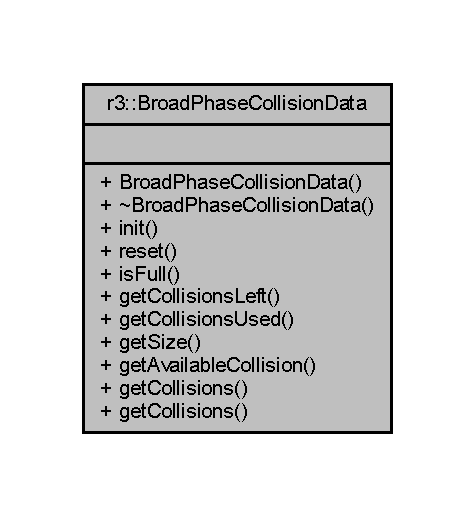
\includegraphics[width=228pt]{classr3_1_1_broad_phase_collision_data__coll__graph}
\end{center}
\end{figure}
\subsection*{Public Member Functions}
\begin{DoxyCompactItemize}
\item 
\mbox{\hyperlink{classr3_1_1_broad_phase_collision_data_a435ccad13c2e1d67f1550e11faf7fa3f}{Broad\+Phase\+Collision\+Data}} (int collisions\+Max=1000, int iterations=0)
\item 
\mbox{\hyperlink{classr3_1_1_broad_phase_collision_data_a54a7831ccec5886c70192159bdd62b0c}{$\sim$\+Broad\+Phase\+Collision\+Data}} ()
\item 
void \mbox{\hyperlink{classr3_1_1_broad_phase_collision_data_a6501b0c4ab0f881b6476332aff03d06b}{init}} (int collisions\+Max, int iterations)
\item 
void \mbox{\hyperlink{classr3_1_1_broad_phase_collision_data_a258a014684e0c480929e8980a40a5ab9}{reset}} ()
\item 
bool \mbox{\hyperlink{classr3_1_1_broad_phase_collision_data_a2a553a4971808f372fc4511bdcd8797c}{is\+Full}} () const
\item 
int \mbox{\hyperlink{classr3_1_1_broad_phase_collision_data_a3b063cc09bfac0a6a87fb03dccef16a9}{get\+Collisions\+Left}} () const
\item 
int \mbox{\hyperlink{classr3_1_1_broad_phase_collision_data_acdcf9e658532adf83d51f6cb01d82a16}{get\+Collisions\+Used}} () const
\item 
int \mbox{\hyperlink{classr3_1_1_broad_phase_collision_data_a6ec1a2db157093ffa0fb790dbf82907e}{get\+Size}} () const
\item 
\mbox{\hyperlink{structr3_1_1_collision_pair}{Collision\+Pair}} $\ast$ \mbox{\hyperlink{classr3_1_1_broad_phase_collision_data_a896087f6429507bdd382425c6ffd8ca6}{get\+Available\+Collision}} ()
\item 
std\+::vector$<$ \mbox{\hyperlink{structr3_1_1_collision_pair}{Collision\+Pair}} $>$ \& \mbox{\hyperlink{classr3_1_1_broad_phase_collision_data_a980b5929f5717557bf2b145478a25e86}{get\+Collisions}} ()
\item 
const std\+::vector$<$ \mbox{\hyperlink{structr3_1_1_collision_pair}{Collision\+Pair}} $>$ \& \mbox{\hyperlink{classr3_1_1_broad_phase_collision_data_a2096507a5422a1fb3ba213a2638f9143}{get\+Collisions}} () const
\end{DoxyCompactItemize}


\subsection{Constructor \& Destructor Documentation}
\mbox{\Hypertarget{classr3_1_1_broad_phase_collision_data_a435ccad13c2e1d67f1550e11faf7fa3f}\label{classr3_1_1_broad_phase_collision_data_a435ccad13c2e1d67f1550e11faf7fa3f}} 
\index{r3\+::\+Broad\+Phase\+Collision\+Data@{r3\+::\+Broad\+Phase\+Collision\+Data}!Broad\+Phase\+Collision\+Data@{Broad\+Phase\+Collision\+Data}}
\index{Broad\+Phase\+Collision\+Data@{Broad\+Phase\+Collision\+Data}!r3\+::\+Broad\+Phase\+Collision\+Data@{r3\+::\+Broad\+Phase\+Collision\+Data}}
\subsubsection{\texorpdfstring{Broad\+Phase\+Collision\+Data()}{BroadPhaseCollisionData()}}
{\footnotesize\ttfamily r3\+::\+Broad\+Phase\+Collision\+Data\+::\+Broad\+Phase\+Collision\+Data (\begin{DoxyParamCaption}\item[{int}]{collisions\+Max = {\ttfamily 1000},  }\item[{int}]{iterations = {\ttfamily 0} }\end{DoxyParamCaption})\hspace{0.3cm}{\ttfamily [explicit]}}

\mbox{\Hypertarget{classr3_1_1_broad_phase_collision_data_a54a7831ccec5886c70192159bdd62b0c}\label{classr3_1_1_broad_phase_collision_data_a54a7831ccec5886c70192159bdd62b0c}} 
\index{r3\+::\+Broad\+Phase\+Collision\+Data@{r3\+::\+Broad\+Phase\+Collision\+Data}!````~Broad\+Phase\+Collision\+Data@{$\sim$\+Broad\+Phase\+Collision\+Data}}
\index{````~Broad\+Phase\+Collision\+Data@{$\sim$\+Broad\+Phase\+Collision\+Data}!r3\+::\+Broad\+Phase\+Collision\+Data@{r3\+::\+Broad\+Phase\+Collision\+Data}}
\subsubsection{\texorpdfstring{$\sim$\+Broad\+Phase\+Collision\+Data()}{~BroadPhaseCollisionData()}}
{\footnotesize\ttfamily r3\+::\+Broad\+Phase\+Collision\+Data\+::$\sim$\+Broad\+Phase\+Collision\+Data (\begin{DoxyParamCaption}{ }\end{DoxyParamCaption})\hspace{0.3cm}{\ttfamily [default]}}



\subsection{Member Function Documentation}
\mbox{\Hypertarget{classr3_1_1_broad_phase_collision_data_a896087f6429507bdd382425c6ffd8ca6}\label{classr3_1_1_broad_phase_collision_data_a896087f6429507bdd382425c6ffd8ca6}} 
\index{r3\+::\+Broad\+Phase\+Collision\+Data@{r3\+::\+Broad\+Phase\+Collision\+Data}!get\+Available\+Collision@{get\+Available\+Collision}}
\index{get\+Available\+Collision@{get\+Available\+Collision}!r3\+::\+Broad\+Phase\+Collision\+Data@{r3\+::\+Broad\+Phase\+Collision\+Data}}
\subsubsection{\texorpdfstring{get\+Available\+Collision()}{getAvailableCollision()}}
{\footnotesize\ttfamily \mbox{\hyperlink{structr3_1_1_collision_pair}{Collision\+Pair}} $\ast$ r3\+::\+Broad\+Phase\+Collision\+Data\+::get\+Available\+Collision (\begin{DoxyParamCaption}{ }\end{DoxyParamCaption})}

Get the next available collision. Automatically uses it! \mbox{\Hypertarget{classr3_1_1_broad_phase_collision_data_a980b5929f5717557bf2b145478a25e86}\label{classr3_1_1_broad_phase_collision_data_a980b5929f5717557bf2b145478a25e86}} 
\index{r3\+::\+Broad\+Phase\+Collision\+Data@{r3\+::\+Broad\+Phase\+Collision\+Data}!get\+Collisions@{get\+Collisions}}
\index{get\+Collisions@{get\+Collisions}!r3\+::\+Broad\+Phase\+Collision\+Data@{r3\+::\+Broad\+Phase\+Collision\+Data}}
\subsubsection{\texorpdfstring{get\+Collisions()}{getCollisions()}\hspace{0.1cm}{\footnotesize\ttfamily [1/2]}}
{\footnotesize\ttfamily std\+::vector$<$ \mbox{\hyperlink{structr3_1_1_collision_pair}{Collision\+Pair}} $>$ \& r3\+::\+Broad\+Phase\+Collision\+Data\+::get\+Collisions (\begin{DoxyParamCaption}{ }\end{DoxyParamCaption})}

Get all collision pairs (even collisions that are not in use!) \mbox{\Hypertarget{classr3_1_1_broad_phase_collision_data_a2096507a5422a1fb3ba213a2638f9143}\label{classr3_1_1_broad_phase_collision_data_a2096507a5422a1fb3ba213a2638f9143}} 
\index{r3\+::\+Broad\+Phase\+Collision\+Data@{r3\+::\+Broad\+Phase\+Collision\+Data}!get\+Collisions@{get\+Collisions}}
\index{get\+Collisions@{get\+Collisions}!r3\+::\+Broad\+Phase\+Collision\+Data@{r3\+::\+Broad\+Phase\+Collision\+Data}}
\subsubsection{\texorpdfstring{get\+Collisions()}{getCollisions()}\hspace{0.1cm}{\footnotesize\ttfamily [2/2]}}
{\footnotesize\ttfamily const std\+::vector$<$ \mbox{\hyperlink{structr3_1_1_collision_pair}{Collision\+Pair}} $>$ \& r3\+::\+Broad\+Phase\+Collision\+Data\+::get\+Collisions (\begin{DoxyParamCaption}{ }\end{DoxyParamCaption}) const}

Get all collision pairs (even collisions that are not in use!) \mbox{\Hypertarget{classr3_1_1_broad_phase_collision_data_a3b063cc09bfac0a6a87fb03dccef16a9}\label{classr3_1_1_broad_phase_collision_data_a3b063cc09bfac0a6a87fb03dccef16a9}} 
\index{r3\+::\+Broad\+Phase\+Collision\+Data@{r3\+::\+Broad\+Phase\+Collision\+Data}!get\+Collisions\+Left@{get\+Collisions\+Left}}
\index{get\+Collisions\+Left@{get\+Collisions\+Left}!r3\+::\+Broad\+Phase\+Collision\+Data@{r3\+::\+Broad\+Phase\+Collision\+Data}}
\subsubsection{\texorpdfstring{get\+Collisions\+Left()}{getCollisionsLeft()}}
{\footnotesize\ttfamily int r3\+::\+Broad\+Phase\+Collision\+Data\+::get\+Collisions\+Left (\begin{DoxyParamCaption}{ }\end{DoxyParamCaption}) const}

Check how many collision pairs can still be inserted. \mbox{\Hypertarget{classr3_1_1_broad_phase_collision_data_acdcf9e658532adf83d51f6cb01d82a16}\label{classr3_1_1_broad_phase_collision_data_acdcf9e658532adf83d51f6cb01d82a16}} 
\index{r3\+::\+Broad\+Phase\+Collision\+Data@{r3\+::\+Broad\+Phase\+Collision\+Data}!get\+Collisions\+Used@{get\+Collisions\+Used}}
\index{get\+Collisions\+Used@{get\+Collisions\+Used}!r3\+::\+Broad\+Phase\+Collision\+Data@{r3\+::\+Broad\+Phase\+Collision\+Data}}
\subsubsection{\texorpdfstring{get\+Collisions\+Used()}{getCollisionsUsed()}}
{\footnotesize\ttfamily int r3\+::\+Broad\+Phase\+Collision\+Data\+::get\+Collisions\+Used (\begin{DoxyParamCaption}{ }\end{DoxyParamCaption}) const}

Check how many collision pairs have been inserted. \mbox{\Hypertarget{classr3_1_1_broad_phase_collision_data_a6ec1a2db157093ffa0fb790dbf82907e}\label{classr3_1_1_broad_phase_collision_data_a6ec1a2db157093ffa0fb790dbf82907e}} 
\index{r3\+::\+Broad\+Phase\+Collision\+Data@{r3\+::\+Broad\+Phase\+Collision\+Data}!get\+Size@{get\+Size}}
\index{get\+Size@{get\+Size}!r3\+::\+Broad\+Phase\+Collision\+Data@{r3\+::\+Broad\+Phase\+Collision\+Data}}
\subsubsection{\texorpdfstring{get\+Size()}{getSize()}}
{\footnotesize\ttfamily int r3\+::\+Broad\+Phase\+Collision\+Data\+::get\+Size (\begin{DoxyParamCaption}{ }\end{DoxyParamCaption}) const}

Get the maximal number of collisions. \mbox{\Hypertarget{classr3_1_1_broad_phase_collision_data_a6501b0c4ab0f881b6476332aff03d06b}\label{classr3_1_1_broad_phase_collision_data_a6501b0c4ab0f881b6476332aff03d06b}} 
\index{r3\+::\+Broad\+Phase\+Collision\+Data@{r3\+::\+Broad\+Phase\+Collision\+Data}!init@{init}}
\index{init@{init}!r3\+::\+Broad\+Phase\+Collision\+Data@{r3\+::\+Broad\+Phase\+Collision\+Data}}
\subsubsection{\texorpdfstring{init()}{init()}}
{\footnotesize\ttfamily void r3\+::\+Broad\+Phase\+Collision\+Data\+::init (\begin{DoxyParamCaption}\item[{int}]{collisions\+Max,  }\item[{int}]{iterations }\end{DoxyParamCaption})}

Set the maximal number of used collisions. \mbox{\Hypertarget{classr3_1_1_broad_phase_collision_data_a2a553a4971808f372fc4511bdcd8797c}\label{classr3_1_1_broad_phase_collision_data_a2a553a4971808f372fc4511bdcd8797c}} 
\index{r3\+::\+Broad\+Phase\+Collision\+Data@{r3\+::\+Broad\+Phase\+Collision\+Data}!is\+Full@{is\+Full}}
\index{is\+Full@{is\+Full}!r3\+::\+Broad\+Phase\+Collision\+Data@{r3\+::\+Broad\+Phase\+Collision\+Data}}
\subsubsection{\texorpdfstring{is\+Full()}{isFull()}}
{\footnotesize\ttfamily bool r3\+::\+Broad\+Phase\+Collision\+Data\+::is\+Full (\begin{DoxyParamCaption}{ }\end{DoxyParamCaption}) const}

Check if there is no more room for new contacts. \mbox{\Hypertarget{classr3_1_1_broad_phase_collision_data_a258a014684e0c480929e8980a40a5ab9}\label{classr3_1_1_broad_phase_collision_data_a258a014684e0c480929e8980a40a5ab9}} 
\index{r3\+::\+Broad\+Phase\+Collision\+Data@{r3\+::\+Broad\+Phase\+Collision\+Data}!reset@{reset}}
\index{reset@{reset}!r3\+::\+Broad\+Phase\+Collision\+Data@{r3\+::\+Broad\+Phase\+Collision\+Data}}
\subsubsection{\texorpdfstring{reset()}{reset()}}
{\footnotesize\ttfamily void r3\+::\+Broad\+Phase\+Collision\+Data\+::reset (\begin{DoxyParamCaption}{ }\end{DoxyParamCaption})}

Reset the number of used collisions. 

The documentation for this class was generated from the following files\+:\begin{DoxyCompactItemize}
\item 
D\+:/\+Library/\+Documents/\+Job/\+Forschungsmaster/\+Projekte/\+Simulation\+Visualization/\+Rumble3\+D/\+Rumble3\+D/include/\+R3\+D/\+Rigid\+Body\+Engine/\+Collision\+Detection/\mbox{\hyperlink{_broad_phase_collision_data_8h}{Broad\+Phase\+Collision\+Data.\+h}}\item 
D\+:/\+Library/\+Documents/\+Job/\+Forschungsmaster/\+Projekte/\+Simulation\+Visualization/\+Rumble3\+D/\+Rumble3\+D/src/\+Rigid\+Body\+Engine/\+Collision\+Detection/\mbox{\hyperlink{_broad_phase_collision_data_8cpp}{Broad\+Phase\+Collision\+Data.\+cpp}}\end{DoxyCompactItemize}

\hypertarget{classr3_1_1_broad_phase_filter}{}\section{r3\+:\+:Broad\+Phase\+Filter Class Reference}
\label{classr3_1_1_broad_phase_filter}\index{r3\+::\+Broad\+Phase\+Filter@{r3\+::\+Broad\+Phase\+Filter}}


Default implementation of \mbox{\hyperlink{classr3_1_1_i_broad_phase_filter}{I\+Broad\+Phase\+Filter}}.  




{\ttfamily \#include $<$Broad\+Phase\+Filter.\+h$>$}



Inheritance diagram for r3\+:\+:Broad\+Phase\+Filter\+:\nopagebreak
\begin{figure}[H]
\begin{center}
\leavevmode
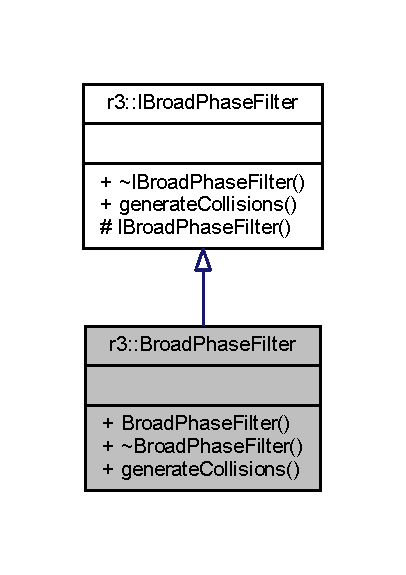
\includegraphics[width=195pt]{classr3_1_1_broad_phase_filter__inherit__graph}
\end{center}
\end{figure}


Collaboration diagram for r3\+:\+:Broad\+Phase\+Filter\+:\nopagebreak
\begin{figure}[H]
\begin{center}
\leavevmode
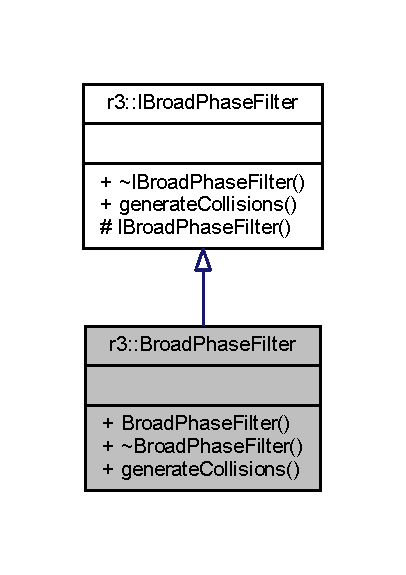
\includegraphics[width=195pt]{classr3_1_1_broad_phase_filter__coll__graph}
\end{center}
\end{figure}
\subsection*{Public Member Functions}
\begin{DoxyCompactItemize}
\item 
\mbox{\hyperlink{classr3_1_1_broad_phase_filter_afcdb0ed5acb941bf16e284cb0031fe2e}{Broad\+Phase\+Filter}} ()
\item 
\mbox{\hyperlink{classr3_1_1_broad_phase_filter_a3c28ac36ed06766b235efad77ff9fd5d}{$\sim$\+Broad\+Phase\+Filter}} ()
\item 
void \mbox{\hyperlink{classr3_1_1_broad_phase_filter_a0435dc6468401e32bf151f84f52e80f8}{generate\+Collisions}} (const std\+::vector$<$ \mbox{\hyperlink{classr3_1_1_rigid_body}{Rigid\+Body}} $\ast$$>$ \&rigid\+Bodies, \mbox{\hyperlink{classr3_1_1_fixed_size_container}{Fixed\+Size\+Container}}$<$ \mbox{\hyperlink{classr3_1_1_collision_pair}{Collision\+Pair}} $>$ \&data) override
\begin{DoxyCompactList}\small\item\em Conservatively check, which rigid body pairs might collide. These collisions can be false positives, but there should never be false negatives. \end{DoxyCompactList}\end{DoxyCompactItemize}
\subsection*{Additional Inherited Members}


\subsection{Detailed Description}
Default implementation of \mbox{\hyperlink{classr3_1_1_i_broad_phase_filter}{I\+Broad\+Phase\+Filter}}. 

\subsection{Constructor \& Destructor Documentation}
\mbox{\Hypertarget{classr3_1_1_broad_phase_filter_afcdb0ed5acb941bf16e284cb0031fe2e}\label{classr3_1_1_broad_phase_filter_afcdb0ed5acb941bf16e284cb0031fe2e}} 
\index{r3\+::\+Broad\+Phase\+Filter@{r3\+::\+Broad\+Phase\+Filter}!Broad\+Phase\+Filter@{Broad\+Phase\+Filter}}
\index{Broad\+Phase\+Filter@{Broad\+Phase\+Filter}!r3\+::\+Broad\+Phase\+Filter@{r3\+::\+Broad\+Phase\+Filter}}
\subsubsection{\texorpdfstring{Broad\+Phase\+Filter()}{BroadPhaseFilter()}}
{\footnotesize\ttfamily r3\+::\+Broad\+Phase\+Filter\+::\+Broad\+Phase\+Filter (\begin{DoxyParamCaption}{ }\end{DoxyParamCaption})\hspace{0.3cm}{\ttfamily [explicit]}, {\ttfamily [default]}}

\mbox{\Hypertarget{classr3_1_1_broad_phase_filter_a3c28ac36ed06766b235efad77ff9fd5d}\label{classr3_1_1_broad_phase_filter_a3c28ac36ed06766b235efad77ff9fd5d}} 
\index{r3\+::\+Broad\+Phase\+Filter@{r3\+::\+Broad\+Phase\+Filter}!````~Broad\+Phase\+Filter@{$\sim$\+Broad\+Phase\+Filter}}
\index{````~Broad\+Phase\+Filter@{$\sim$\+Broad\+Phase\+Filter}!r3\+::\+Broad\+Phase\+Filter@{r3\+::\+Broad\+Phase\+Filter}}
\subsubsection{\texorpdfstring{$\sim$\+Broad\+Phase\+Filter()}{~BroadPhaseFilter()}}
{\footnotesize\ttfamily r3\+::\+Broad\+Phase\+Filter\+::$\sim$\+Broad\+Phase\+Filter (\begin{DoxyParamCaption}{ }\end{DoxyParamCaption})\hspace{0.3cm}{\ttfamily [default]}}



\subsection{Member Function Documentation}
\mbox{\Hypertarget{classr3_1_1_broad_phase_filter_a0435dc6468401e32bf151f84f52e80f8}\label{classr3_1_1_broad_phase_filter_a0435dc6468401e32bf151f84f52e80f8}} 
\index{r3\+::\+Broad\+Phase\+Filter@{r3\+::\+Broad\+Phase\+Filter}!generate\+Collisions@{generate\+Collisions}}
\index{generate\+Collisions@{generate\+Collisions}!r3\+::\+Broad\+Phase\+Filter@{r3\+::\+Broad\+Phase\+Filter}}
\subsubsection{\texorpdfstring{generate\+Collisions()}{generateCollisions()}}
{\footnotesize\ttfamily void r3\+::\+Broad\+Phase\+Filter\+::generate\+Collisions (\begin{DoxyParamCaption}\item[{const std\+::vector$<$ \mbox{\hyperlink{classr3_1_1_rigid_body}{Rigid\+Body}} $\ast$$>$ \&}]{rigid\+Bodies,  }\item[{\mbox{\hyperlink{classr3_1_1_fixed_size_container}{Fixed\+Size\+Container}}$<$ \mbox{\hyperlink{classr3_1_1_collision_pair}{Collision\+Pair}} $>$ \&}]{data }\end{DoxyParamCaption})\hspace{0.3cm}{\ttfamily [override]}, {\ttfamily [virtual]}}



Conservatively check, which rigid body pairs might collide. These collisions can be false positives, but there should never be false negatives. 


\begin{DoxyParams}[1]{Parameters}
 & {\em rigid\+Bodies} & The rigid bodies to check against possible collisions. \\
\hline
\mbox{\tt out}  & {\em data} & A number of possible collisions. \\
\hline
\end{DoxyParams}
\begin{DoxyRefDesc}{Todo}
\item[\mbox{\hyperlink{todo__todo000013}{Todo}}]use rigid body mask and layout \end{DoxyRefDesc}


Implements \mbox{\hyperlink{classr3_1_1_i_broad_phase_filter_a5f437f6390a8f10bf96d72e35e3b4432}{r3\+::\+I\+Broad\+Phase\+Filter}}.



The documentation for this class was generated from the following files\+:\begin{DoxyCompactItemize}
\item 
D\+:/\+Library/\+Documents/\+Job/\+Forschungsmaster/\+Projekte/\+Simulation\+Visualization/\+Rumble3\+D/\+Rumble3\+D/include/\+R3\+D/\+Rigid\+Body\+Engine/\+Collision\+Detection/\mbox{\hyperlink{_broad_phase_filter_8h}{Broad\+Phase\+Filter.\+h}}\item 
D\+:/\+Library/\+Documents/\+Job/\+Forschungsmaster/\+Projekte/\+Simulation\+Visualization/\+Rumble3\+D/\+Rumble3\+D/src/\+Rigid\+Body\+Engine/\+Collision\+Detection/\mbox{\hyperlink{_broad_phase_filter_8cpp}{Broad\+Phase\+Filter.\+cpp}}\end{DoxyCompactItemize}

\hypertarget{classr3_1_1_b_v_h_node}{}\section{r3\+:\+:B\+V\+H\+Node$<$ Bounding\+Volume\+Class $>$ Class Template Reference}
\label{classr3_1_1_b_v_h_node}\index{r3\+::\+B\+V\+H\+Node$<$ Bounding\+Volume\+Class $>$@{r3\+::\+B\+V\+H\+Node$<$ Bounding\+Volume\+Class $>$}}


{\ttfamily \#include $<$B\+V\+H\+Node.\+h$>$}



Collaboration diagram for r3\+:\+:B\+V\+H\+Node$<$ Bounding\+Volume\+Class $>$\+:\nopagebreak
\begin{figure}[H]
\begin{center}
\leavevmode
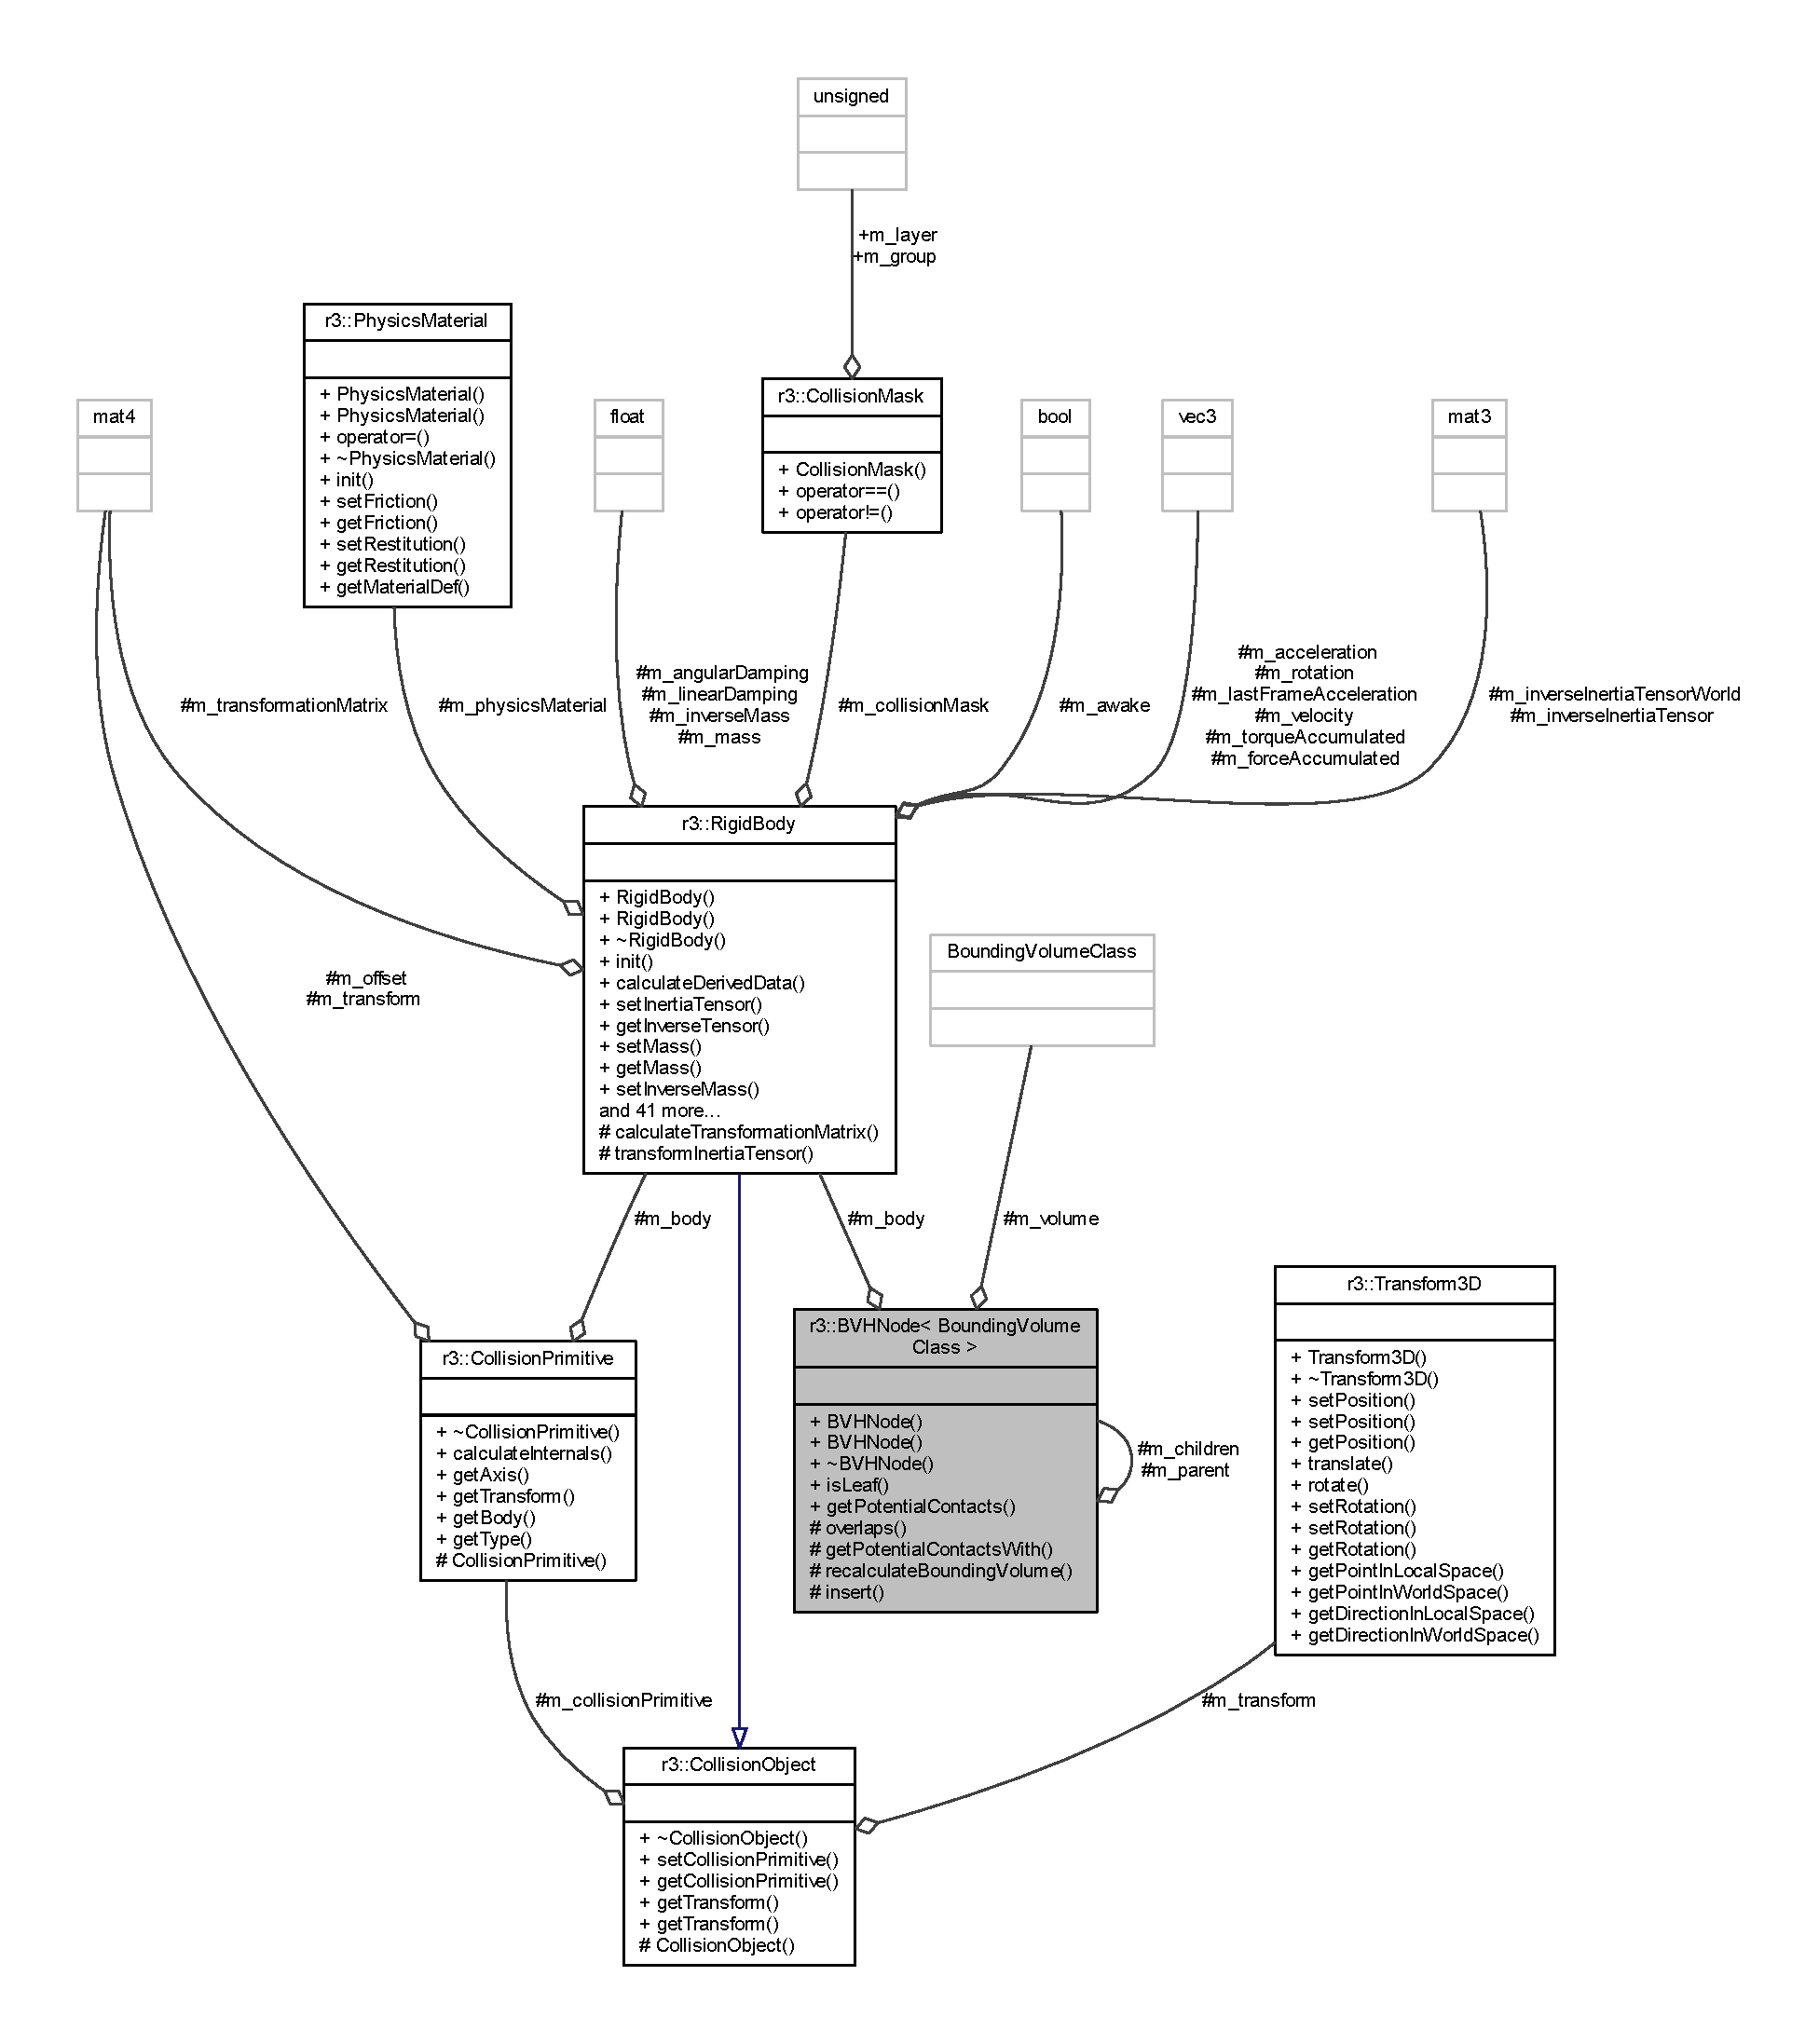
\includegraphics[width=350pt]{classr3_1_1_b_v_h_node__coll__graph}
\end{center}
\end{figure}
\subsection*{Public Member Functions}
\begin{DoxyCompactItemize}
\item 
\mbox{\hyperlink{classr3_1_1_b_v_h_node_a31b8beb2d10f5df915be92eab4bdd7f6}{B\+V\+H\+Node}} ()
\item 
\mbox{\hyperlink{classr3_1_1_b_v_h_node_a983ae7d4ab515427436692b8a846da6f}{B\+V\+H\+Node}} (\mbox{\hyperlink{classr3_1_1_b_v_h_node}{B\+V\+H\+Node}}$<$ Bounding\+Volume\+Class $>$ $\ast$parent, const Bounding\+Volume\+Class \&volume, \mbox{\hyperlink{classr3_1_1_rigid_body}{Rigid\+Body}} $\ast$body=nullptr)
\item 
\mbox{\hyperlink{classr3_1_1_b_v_h_node_a72194bd522058bfd362b0ab77c0303af}{$\sim$\+B\+V\+H\+Node}} ()
\item 
bool \mbox{\hyperlink{classr3_1_1_b_v_h_node_a517b40f1a91cda371b3cb786f1c7e155}{is\+Leaf}} () const
\begin{DoxyCompactList}\small\item\em Check if this node is a leaf node (= has no child nodes). \end{DoxyCompactList}\item 
unsigned \mbox{\hyperlink{classr3_1_1_b_v_h_node_a9a8083e409cd4452e25878e80283440f}{get\+Potential\+Contacts}} (\mbox{\hyperlink{classr3_1_1_collision_pair}{Collision\+Pair}} $\ast$contacts, unsigned limit) const
\end{DoxyCompactItemize}
\subsection*{Protected Member Functions}
\begin{DoxyCompactItemize}
\item 
bool \mbox{\hyperlink{classr3_1_1_b_v_h_node_a69ec6f958bbe07629cd979599532dfd8}{overlaps}} (\mbox{\hyperlink{classr3_1_1_b_v_h_node}{B\+V\+H\+Node}}$<$ Bounding\+Volume\+Class $>$ $\ast$other) const
\item 
unsigned \mbox{\hyperlink{classr3_1_1_b_v_h_node_abf81453da8179650565a0a5379ccb5cb}{get\+Potential\+Contacts\+With}} (\mbox{\hyperlink{classr3_1_1_b_v_h_node}{B\+V\+H\+Node}}$<$ Bounding\+Volume\+Class $>$ $\ast$other, \mbox{\hyperlink{classr3_1_1_collision_pair}{Collision\+Pair}} $\ast$contacts, unsigned limit) const
\item 
void \mbox{\hyperlink{classr3_1_1_b_v_h_node_a52539a0d78d758021a2fe4bedd30e671}{recalculate\+Bounding\+Volume}} ()
\item 
void \mbox{\hyperlink{classr3_1_1_b_v_h_node_ab6f91727e36689a7edc9f8c168ab904b}{insert}} (\mbox{\hyperlink{classr3_1_1_rigid_body}{Rigid\+Body}} $\ast$new\+Body, const Bounding\+Volume\+Class \&new\+Volume)
\end{DoxyCompactItemize}
\subsection*{Protected Attributes}
\begin{DoxyCompactItemize}
\item 
\mbox{\hyperlink{classr3_1_1_b_v_h_node}{B\+V\+H\+Node}} $\ast$ \mbox{\hyperlink{classr3_1_1_b_v_h_node_a62424473dd79cf59262a6a53995b0e26}{m\+\_\+parent}}
\item 
\mbox{\hyperlink{classr3_1_1_b_v_h_node}{B\+V\+H\+Node}} $\ast$ \mbox{\hyperlink{classr3_1_1_b_v_h_node_ac3df92e9a175e4037a07801e1cca73db}{m\+\_\+children}} \mbox{[}2\mbox{]}
\item 
\mbox{\hyperlink{classr3_1_1_rigid_body}{Rigid\+Body}} $\ast$ \mbox{\hyperlink{classr3_1_1_b_v_h_node_a7f1a7f51f17ed00cc39298ff4d1f1d57}{m\+\_\+body}}
\item 
Bounding\+Volume\+Class \mbox{\hyperlink{classr3_1_1_b_v_h_node_a114366b1f5cbb56f6f650f9c794258a7}{m\+\_\+volume}}
\end{DoxyCompactItemize}


\subsection{Constructor \& Destructor Documentation}
\mbox{\Hypertarget{classr3_1_1_b_v_h_node_a31b8beb2d10f5df915be92eab4bdd7f6}\label{classr3_1_1_b_v_h_node_a31b8beb2d10f5df915be92eab4bdd7f6}} 
\index{r3\+::\+B\+V\+H\+Node@{r3\+::\+B\+V\+H\+Node}!B\+V\+H\+Node@{B\+V\+H\+Node}}
\index{B\+V\+H\+Node@{B\+V\+H\+Node}!r3\+::\+B\+V\+H\+Node@{r3\+::\+B\+V\+H\+Node}}
\subsubsection{\texorpdfstring{B\+V\+H\+Node()}{BVHNode()}\hspace{0.1cm}{\footnotesize\ttfamily [1/2]}}
{\footnotesize\ttfamily template$<$class Bounding\+Volume\+Class $>$ \\
\mbox{\hyperlink{classr3_1_1_b_v_h_node}{r3\+::\+B\+V\+H\+Node}}$<$ Bounding\+Volume\+Class $>$\+::\mbox{\hyperlink{classr3_1_1_b_v_h_node}{B\+V\+H\+Node}} (\begin{DoxyParamCaption}{ }\end{DoxyParamCaption})\hspace{0.3cm}{\ttfamily [default]}}

\mbox{\Hypertarget{classr3_1_1_b_v_h_node_a983ae7d4ab515427436692b8a846da6f}\label{classr3_1_1_b_v_h_node_a983ae7d4ab515427436692b8a846da6f}} 
\index{r3\+::\+B\+V\+H\+Node@{r3\+::\+B\+V\+H\+Node}!B\+V\+H\+Node@{B\+V\+H\+Node}}
\index{B\+V\+H\+Node@{B\+V\+H\+Node}!r3\+::\+B\+V\+H\+Node@{r3\+::\+B\+V\+H\+Node}}
\subsubsection{\texorpdfstring{B\+V\+H\+Node()}{BVHNode()}\hspace{0.1cm}{\footnotesize\ttfamily [2/2]}}
{\footnotesize\ttfamily template$<$class Bounding\+Volume\+Class $>$ \\
\mbox{\hyperlink{classr3_1_1_b_v_h_node}{r3\+::\+B\+V\+H\+Node}}$<$ Bounding\+Volume\+Class $>$\+::\mbox{\hyperlink{classr3_1_1_b_v_h_node}{B\+V\+H\+Node}} (\begin{DoxyParamCaption}\item[{\mbox{\hyperlink{classr3_1_1_b_v_h_node}{B\+V\+H\+Node}}$<$ Bounding\+Volume\+Class $>$ $\ast$}]{parent,  }\item[{const Bounding\+Volume\+Class \&}]{volume,  }\item[{\mbox{\hyperlink{classr3_1_1_rigid_body}{Rigid\+Body}} $\ast$}]{body = {\ttfamily nullptr} }\end{DoxyParamCaption})}

\mbox{\Hypertarget{classr3_1_1_b_v_h_node_a72194bd522058bfd362b0ab77c0303af}\label{classr3_1_1_b_v_h_node_a72194bd522058bfd362b0ab77c0303af}} 
\index{r3\+::\+B\+V\+H\+Node@{r3\+::\+B\+V\+H\+Node}!````~B\+V\+H\+Node@{$\sim$\+B\+V\+H\+Node}}
\index{````~B\+V\+H\+Node@{$\sim$\+B\+V\+H\+Node}!r3\+::\+B\+V\+H\+Node@{r3\+::\+B\+V\+H\+Node}}
\subsubsection{\texorpdfstring{$\sim$\+B\+V\+H\+Node()}{~BVHNode()}}
{\footnotesize\ttfamily template$<$class Bounding\+Volume\+Class $>$ \\
\mbox{\hyperlink{classr3_1_1_b_v_h_node}{r3\+::\+B\+V\+H\+Node}}$<$ Bounding\+Volume\+Class $>$\+::$\sim$\mbox{\hyperlink{classr3_1_1_b_v_h_node}{B\+V\+H\+Node}} (\begin{DoxyParamCaption}{ }\end{DoxyParamCaption})}



\subsection{Member Function Documentation}
\mbox{\Hypertarget{classr3_1_1_b_v_h_node_a9a8083e409cd4452e25878e80283440f}\label{classr3_1_1_b_v_h_node_a9a8083e409cd4452e25878e80283440f}} 
\index{r3\+::\+B\+V\+H\+Node@{r3\+::\+B\+V\+H\+Node}!get\+Potential\+Contacts@{get\+Potential\+Contacts}}
\index{get\+Potential\+Contacts@{get\+Potential\+Contacts}!r3\+::\+B\+V\+H\+Node@{r3\+::\+B\+V\+H\+Node}}
\subsubsection{\texorpdfstring{get\+Potential\+Contacts()}{getPotentialContacts()}}
{\footnotesize\ttfamily template$<$class Bounding\+Volume\+Class $>$ \\
unsigned \mbox{\hyperlink{classr3_1_1_b_v_h_node}{r3\+::\+B\+V\+H\+Node}}$<$ Bounding\+Volume\+Class $>$\+::get\+Potential\+Contacts (\begin{DoxyParamCaption}\item[{\mbox{\hyperlink{classr3_1_1_collision_pair}{Collision\+Pair}} $\ast$}]{contacts,  }\item[{unsigned}]{limit }\end{DoxyParamCaption}) const}

\mbox{\Hypertarget{classr3_1_1_b_v_h_node_abf81453da8179650565a0a5379ccb5cb}\label{classr3_1_1_b_v_h_node_abf81453da8179650565a0a5379ccb5cb}} 
\index{r3\+::\+B\+V\+H\+Node@{r3\+::\+B\+V\+H\+Node}!get\+Potential\+Contacts\+With@{get\+Potential\+Contacts\+With}}
\index{get\+Potential\+Contacts\+With@{get\+Potential\+Contacts\+With}!r3\+::\+B\+V\+H\+Node@{r3\+::\+B\+V\+H\+Node}}
\subsubsection{\texorpdfstring{get\+Potential\+Contacts\+With()}{getPotentialContactsWith()}}
{\footnotesize\ttfamily template$<$class Bounding\+Volume\+Class $>$ \\
unsigned \mbox{\hyperlink{classr3_1_1_b_v_h_node}{r3\+::\+B\+V\+H\+Node}}$<$ Bounding\+Volume\+Class $>$\+::get\+Potential\+Contacts\+With (\begin{DoxyParamCaption}\item[{\mbox{\hyperlink{classr3_1_1_b_v_h_node}{B\+V\+H\+Node}}$<$ Bounding\+Volume\+Class $>$ $\ast$}]{other,  }\item[{\mbox{\hyperlink{classr3_1_1_collision_pair}{Collision\+Pair}} $\ast$}]{contacts,  }\item[{unsigned}]{limit }\end{DoxyParamCaption}) const\hspace{0.3cm}{\ttfamily [protected]}}

\mbox{\Hypertarget{classr3_1_1_b_v_h_node_ab6f91727e36689a7edc9f8c168ab904b}\label{classr3_1_1_b_v_h_node_ab6f91727e36689a7edc9f8c168ab904b}} 
\index{r3\+::\+B\+V\+H\+Node@{r3\+::\+B\+V\+H\+Node}!insert@{insert}}
\index{insert@{insert}!r3\+::\+B\+V\+H\+Node@{r3\+::\+B\+V\+H\+Node}}
\subsubsection{\texorpdfstring{insert()}{insert()}}
{\footnotesize\ttfamily template$<$class Bounding\+Volume\+Class $>$ \\
void \mbox{\hyperlink{classr3_1_1_b_v_h_node}{r3\+::\+B\+V\+H\+Node}}$<$ Bounding\+Volume\+Class $>$\+::insert (\begin{DoxyParamCaption}\item[{\mbox{\hyperlink{classr3_1_1_rigid_body}{Rigid\+Body}} $\ast$}]{new\+Body,  }\item[{const Bounding\+Volume\+Class \&}]{new\+Volume }\end{DoxyParamCaption})\hspace{0.3cm}{\ttfamily [protected]}}

\mbox{\Hypertarget{classr3_1_1_b_v_h_node_a517b40f1a91cda371b3cb786f1c7e155}\label{classr3_1_1_b_v_h_node_a517b40f1a91cda371b3cb786f1c7e155}} 
\index{r3\+::\+B\+V\+H\+Node@{r3\+::\+B\+V\+H\+Node}!is\+Leaf@{is\+Leaf}}
\index{is\+Leaf@{is\+Leaf}!r3\+::\+B\+V\+H\+Node@{r3\+::\+B\+V\+H\+Node}}
\subsubsection{\texorpdfstring{is\+Leaf()}{isLeaf()}}
{\footnotesize\ttfamily template$<$class Bounding\+Volume\+Class $>$ \\
bool \mbox{\hyperlink{classr3_1_1_b_v_h_node}{r3\+::\+B\+V\+H\+Node}}$<$ Bounding\+Volume\+Class $>$\+::is\+Leaf (\begin{DoxyParamCaption}{ }\end{DoxyParamCaption}) const}



Check if this node is a leaf node (= has no child nodes). 

\begin{DoxyReturn}{Returns}
True if it is a leaf node, false otherwise. 
\end{DoxyReturn}
\mbox{\Hypertarget{classr3_1_1_b_v_h_node_a69ec6f958bbe07629cd979599532dfd8}\label{classr3_1_1_b_v_h_node_a69ec6f958bbe07629cd979599532dfd8}} 
\index{r3\+::\+B\+V\+H\+Node@{r3\+::\+B\+V\+H\+Node}!overlaps@{overlaps}}
\index{overlaps@{overlaps}!r3\+::\+B\+V\+H\+Node@{r3\+::\+B\+V\+H\+Node}}
\subsubsection{\texorpdfstring{overlaps()}{overlaps()}}
{\footnotesize\ttfamily template$<$class Bounding\+Volume\+Class $>$ \\
bool \mbox{\hyperlink{classr3_1_1_b_v_h_node}{r3\+::\+B\+V\+H\+Node}}$<$ Bounding\+Volume\+Class $>$\+::overlaps (\begin{DoxyParamCaption}\item[{\mbox{\hyperlink{classr3_1_1_b_v_h_node}{B\+V\+H\+Node}}$<$ Bounding\+Volume\+Class $>$ $\ast$}]{other }\end{DoxyParamCaption}) const\hspace{0.3cm}{\ttfamily [protected]}}

\mbox{\Hypertarget{classr3_1_1_b_v_h_node_a52539a0d78d758021a2fe4bedd30e671}\label{classr3_1_1_b_v_h_node_a52539a0d78d758021a2fe4bedd30e671}} 
\index{r3\+::\+B\+V\+H\+Node@{r3\+::\+B\+V\+H\+Node}!recalculate\+Bounding\+Volume@{recalculate\+Bounding\+Volume}}
\index{recalculate\+Bounding\+Volume@{recalculate\+Bounding\+Volume}!r3\+::\+B\+V\+H\+Node@{r3\+::\+B\+V\+H\+Node}}
\subsubsection{\texorpdfstring{recalculate\+Bounding\+Volume()}{recalculateBoundingVolume()}}
{\footnotesize\ttfamily template$<$class Bounding\+Volume\+Class $>$ \\
void \mbox{\hyperlink{classr3_1_1_b_v_h_node}{r3\+::\+B\+V\+H\+Node}}$<$ Bounding\+Volume\+Class $>$\+::recalculate\+Bounding\+Volume (\begin{DoxyParamCaption}{ }\end{DoxyParamCaption})\hspace{0.3cm}{\ttfamily [protected]}}



\subsection{Member Data Documentation}
\mbox{\Hypertarget{classr3_1_1_b_v_h_node_a7f1a7f51f17ed00cc39298ff4d1f1d57}\label{classr3_1_1_b_v_h_node_a7f1a7f51f17ed00cc39298ff4d1f1d57}} 
\index{r3\+::\+B\+V\+H\+Node@{r3\+::\+B\+V\+H\+Node}!m\+\_\+body@{m\+\_\+body}}
\index{m\+\_\+body@{m\+\_\+body}!r3\+::\+B\+V\+H\+Node@{r3\+::\+B\+V\+H\+Node}}
\subsubsection{\texorpdfstring{m\+\_\+body}{m\_body}}
{\footnotesize\ttfamily template$<$class Bounding\+Volume\+Class$>$ \\
\mbox{\hyperlink{classr3_1_1_rigid_body}{Rigid\+Body}}$\ast$ \mbox{\hyperlink{classr3_1_1_b_v_h_node}{r3\+::\+B\+V\+H\+Node}}$<$ Bounding\+Volume\+Class $>$\+::m\+\_\+body\hspace{0.3cm}{\ttfamily [protected]}}

\mbox{\Hypertarget{classr3_1_1_b_v_h_node_ac3df92e9a175e4037a07801e1cca73db}\label{classr3_1_1_b_v_h_node_ac3df92e9a175e4037a07801e1cca73db}} 
\index{r3\+::\+B\+V\+H\+Node@{r3\+::\+B\+V\+H\+Node}!m\+\_\+children@{m\+\_\+children}}
\index{m\+\_\+children@{m\+\_\+children}!r3\+::\+B\+V\+H\+Node@{r3\+::\+B\+V\+H\+Node}}
\subsubsection{\texorpdfstring{m\+\_\+children}{m\_children}}
{\footnotesize\ttfamily template$<$class Bounding\+Volume\+Class$>$ \\
\mbox{\hyperlink{classr3_1_1_b_v_h_node}{B\+V\+H\+Node}}$\ast$ \mbox{\hyperlink{classr3_1_1_b_v_h_node}{r3\+::\+B\+V\+H\+Node}}$<$ Bounding\+Volume\+Class $>$\+::m\+\_\+children\mbox{[}2\mbox{]}\hspace{0.3cm}{\ttfamily [protected]}}

\mbox{\Hypertarget{classr3_1_1_b_v_h_node_a62424473dd79cf59262a6a53995b0e26}\label{classr3_1_1_b_v_h_node_a62424473dd79cf59262a6a53995b0e26}} 
\index{r3\+::\+B\+V\+H\+Node@{r3\+::\+B\+V\+H\+Node}!m\+\_\+parent@{m\+\_\+parent}}
\index{m\+\_\+parent@{m\+\_\+parent}!r3\+::\+B\+V\+H\+Node@{r3\+::\+B\+V\+H\+Node}}
\subsubsection{\texorpdfstring{m\+\_\+parent}{m\_parent}}
{\footnotesize\ttfamily template$<$class Bounding\+Volume\+Class$>$ \\
\mbox{\hyperlink{classr3_1_1_b_v_h_node}{B\+V\+H\+Node}}$\ast$ \mbox{\hyperlink{classr3_1_1_b_v_h_node}{r3\+::\+B\+V\+H\+Node}}$<$ Bounding\+Volume\+Class $>$\+::m\+\_\+parent\hspace{0.3cm}{\ttfamily [protected]}}

\mbox{\Hypertarget{classr3_1_1_b_v_h_node_a114366b1f5cbb56f6f650f9c794258a7}\label{classr3_1_1_b_v_h_node_a114366b1f5cbb56f6f650f9c794258a7}} 
\index{r3\+::\+B\+V\+H\+Node@{r3\+::\+B\+V\+H\+Node}!m\+\_\+volume@{m\+\_\+volume}}
\index{m\+\_\+volume@{m\+\_\+volume}!r3\+::\+B\+V\+H\+Node@{r3\+::\+B\+V\+H\+Node}}
\subsubsection{\texorpdfstring{m\+\_\+volume}{m\_volume}}
{\footnotesize\ttfamily template$<$class Bounding\+Volume\+Class$>$ \\
Bounding\+Volume\+Class \mbox{\hyperlink{classr3_1_1_b_v_h_node}{r3\+::\+B\+V\+H\+Node}}$<$ Bounding\+Volume\+Class $>$\+::m\+\_\+volume\hspace{0.3cm}{\ttfamily [protected]}}



The documentation for this class was generated from the following files\+:\begin{DoxyCompactItemize}
\item 
D\+:/\+Library/\+Documents/\+Job/\+Forschungsmaster/\+Projekte/\+Simulation\+Visualization/\+Rumble3\+D/\+Rumble3\+D/include/\+R3\+D/\+Rigid\+Body\+Engine/\mbox{\hyperlink{_b_v_h_node_8h}{B\+V\+H\+Node.\+h}}\item 
D\+:/\+Library/\+Documents/\+Job/\+Forschungsmaster/\+Projekte/\+Simulation\+Visualization/\+Rumble3\+D/\+Rumble3\+D/src/\+Rigid\+Body\+Engine/\mbox{\hyperlink{_b_v_h_node_8cpp}{B\+V\+H\+Node.\+cpp}}\end{DoxyCompactItemize}

\hypertarget{classr3_1_1_collision_algorithm_matrix}{}\section{r3\+:\+:Collision\+Algorithm\+Matrix Class Reference}
\label{classr3_1_1_collision_algorithm_matrix}\index{r3\+::\+Collision\+Algorithm\+Matrix@{r3\+::\+Collision\+Algorithm\+Matrix}}


{\ttfamily \#include $<$Collision\+Algorithm\+Matrix.\+h$>$}



Collaboration diagram for r3\+:\+:Collision\+Algorithm\+Matrix\+:\nopagebreak
\begin{figure}[H]
\begin{center}
\leavevmode
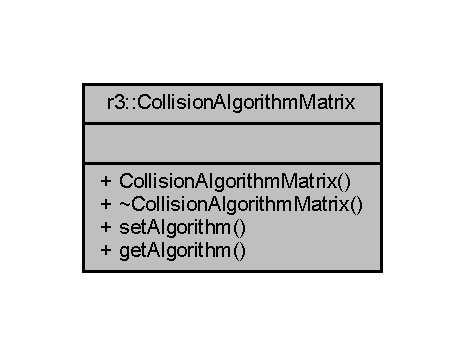
\includegraphics[width=223pt]{classr3_1_1_collision_algorithm_matrix__coll__graph}
\end{center}
\end{figure}
\subsection*{Public Member Functions}
\begin{DoxyCompactItemize}
\item 
\mbox{\hyperlink{classr3_1_1_collision_algorithm_matrix_a97bdad626057f600ae5ffca63eb174b8}{Collision\+Algorithm\+Matrix}} ()
\item 
\mbox{\hyperlink{classr3_1_1_collision_algorithm_matrix_adea2db794d9606ecf24745ad6ac912d8}{$\sim$\+Collision\+Algorithm\+Matrix}} ()
\item 
void \mbox{\hyperlink{classr3_1_1_collision_algorithm_matrix_a6ddf117fbce8a3216b4b4413ccade6d0}{set\+Algorithm}} (\mbox{\hyperlink{classr3_1_1_i_narrow_phase_algorithm}{I\+Narrow\+Phase\+Algorithm}} $\ast$algorithm, Collision\+Primitive\+Type first\+Shape, Collision\+Primitive\+Type second\+Shape)
\item 
\mbox{\hyperlink{classr3_1_1_i_narrow_phase_algorithm}{I\+Narrow\+Phase\+Algorithm}} $\ast$ \mbox{\hyperlink{classr3_1_1_collision_algorithm_matrix_ad40e0f125b95d6bcdb2e8a27c1397e68}{get\+Algorithm}} (Collision\+Primitive\+Type first\+Shape, Collision\+Primitive\+Type second\+Shape)
\end{DoxyCompactItemize}


\subsection{Constructor \& Destructor Documentation}
\mbox{\Hypertarget{classr3_1_1_collision_algorithm_matrix_a97bdad626057f600ae5ffca63eb174b8}\label{classr3_1_1_collision_algorithm_matrix_a97bdad626057f600ae5ffca63eb174b8}} 
\index{r3\+::\+Collision\+Algorithm\+Matrix@{r3\+::\+Collision\+Algorithm\+Matrix}!Collision\+Algorithm\+Matrix@{Collision\+Algorithm\+Matrix}}
\index{Collision\+Algorithm\+Matrix@{Collision\+Algorithm\+Matrix}!r3\+::\+Collision\+Algorithm\+Matrix@{r3\+::\+Collision\+Algorithm\+Matrix}}
\subsubsection{\texorpdfstring{Collision\+Algorithm\+Matrix()}{CollisionAlgorithmMatrix()}}
{\footnotesize\ttfamily r3\+::\+Collision\+Algorithm\+Matrix\+::\+Collision\+Algorithm\+Matrix (\begin{DoxyParamCaption}{ }\end{DoxyParamCaption})\hspace{0.3cm}{\ttfamily [explicit]}}

\mbox{\Hypertarget{classr3_1_1_collision_algorithm_matrix_adea2db794d9606ecf24745ad6ac912d8}\label{classr3_1_1_collision_algorithm_matrix_adea2db794d9606ecf24745ad6ac912d8}} 
\index{r3\+::\+Collision\+Algorithm\+Matrix@{r3\+::\+Collision\+Algorithm\+Matrix}!````~Collision\+Algorithm\+Matrix@{$\sim$\+Collision\+Algorithm\+Matrix}}
\index{````~Collision\+Algorithm\+Matrix@{$\sim$\+Collision\+Algorithm\+Matrix}!r3\+::\+Collision\+Algorithm\+Matrix@{r3\+::\+Collision\+Algorithm\+Matrix}}
\subsubsection{\texorpdfstring{$\sim$\+Collision\+Algorithm\+Matrix()}{~CollisionAlgorithmMatrix()}}
{\footnotesize\ttfamily r3\+::\+Collision\+Algorithm\+Matrix\+::$\sim$\+Collision\+Algorithm\+Matrix (\begin{DoxyParamCaption}{ }\end{DoxyParamCaption})\hspace{0.3cm}{\ttfamily [default]}}



\subsection{Member Function Documentation}
\mbox{\Hypertarget{classr3_1_1_collision_algorithm_matrix_ad40e0f125b95d6bcdb2e8a27c1397e68}\label{classr3_1_1_collision_algorithm_matrix_ad40e0f125b95d6bcdb2e8a27c1397e68}} 
\index{r3\+::\+Collision\+Algorithm\+Matrix@{r3\+::\+Collision\+Algorithm\+Matrix}!get\+Algorithm@{get\+Algorithm}}
\index{get\+Algorithm@{get\+Algorithm}!r3\+::\+Collision\+Algorithm\+Matrix@{r3\+::\+Collision\+Algorithm\+Matrix}}
\subsubsection{\texorpdfstring{get\+Algorithm()}{getAlgorithm()}}
{\footnotesize\ttfamily \mbox{\hyperlink{classr3_1_1_i_narrow_phase_algorithm}{I\+Narrow\+Phase\+Algorithm}} $\ast$ r3\+::\+Collision\+Algorithm\+Matrix\+::get\+Algorithm (\begin{DoxyParamCaption}\item[{Collision\+Primitive\+Type}]{first\+Shape,  }\item[{Collision\+Primitive\+Type}]{second\+Shape }\end{DoxyParamCaption})}

\mbox{\Hypertarget{classr3_1_1_collision_algorithm_matrix_a6ddf117fbce8a3216b4b4413ccade6d0}\label{classr3_1_1_collision_algorithm_matrix_a6ddf117fbce8a3216b4b4413ccade6d0}} 
\index{r3\+::\+Collision\+Algorithm\+Matrix@{r3\+::\+Collision\+Algorithm\+Matrix}!set\+Algorithm@{set\+Algorithm}}
\index{set\+Algorithm@{set\+Algorithm}!r3\+::\+Collision\+Algorithm\+Matrix@{r3\+::\+Collision\+Algorithm\+Matrix}}
\subsubsection{\texorpdfstring{set\+Algorithm()}{setAlgorithm()}}
{\footnotesize\ttfamily void r3\+::\+Collision\+Algorithm\+Matrix\+::set\+Algorithm (\begin{DoxyParamCaption}\item[{\mbox{\hyperlink{classr3_1_1_i_narrow_phase_algorithm}{I\+Narrow\+Phase\+Algorithm}} $\ast$}]{algorithm,  }\item[{Collision\+Primitive\+Type}]{first\+Shape,  }\item[{Collision\+Primitive\+Type}]{second\+Shape }\end{DoxyParamCaption})}



The documentation for this class was generated from the following files\+:\begin{DoxyCompactItemize}
\item 
C\+:/\+Library/\+Job/\+Projekte/\+Simulation\+Visualization/\+Rumble3\+D/\+Rumble3\+D/include/\+R3\+D/\+Rigid\+Body\+Engine/\+Collision\+Detection/\mbox{\hyperlink{_collision_algorithm_matrix_8h}{Collision\+Algorithm\+Matrix.\+h}}\item 
C\+:/\+Library/\+Job/\+Projekte/\+Simulation\+Visualization/\+Rumble3\+D/\+Rumble3\+D/src/\+Rigid\+Body\+Engine/\+Collision\+Detection/\mbox{\hyperlink{_collision_algorithm_matrix_8cpp}{Collision\+Algorithm\+Matrix.\+cpp}}\end{DoxyCompactItemize}

\hypertarget{classr3_1_1_collision_box}{}\section{r3\+:\+:Collision\+Box Class Reference}
\label{classr3_1_1_collision_box}\index{r3\+::\+Collision\+Box@{r3\+::\+Collision\+Box}}


{\ttfamily \#include $<$Collision\+Box.\+h$>$}



Inheritance diagram for r3\+:\+:Collision\+Box\+:\nopagebreak
\begin{figure}[H]
\begin{center}
\leavevmode
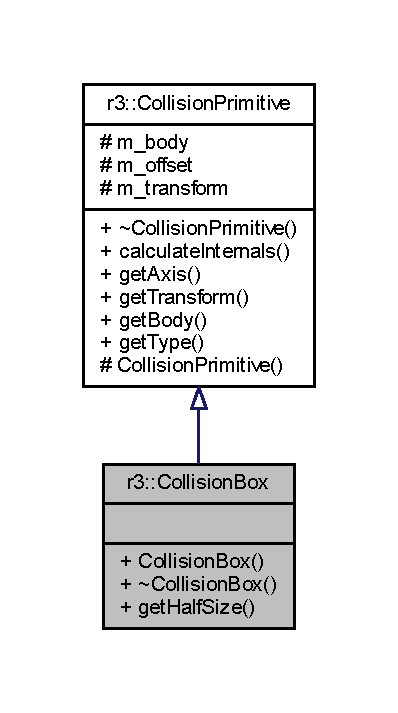
\includegraphics[width=191pt]{classr3_1_1_collision_box__inherit__graph}
\end{center}
\end{figure}


Collaboration diagram for r3\+:\+:Collision\+Box\+:\nopagebreak
\begin{figure}[H]
\begin{center}
\leavevmode
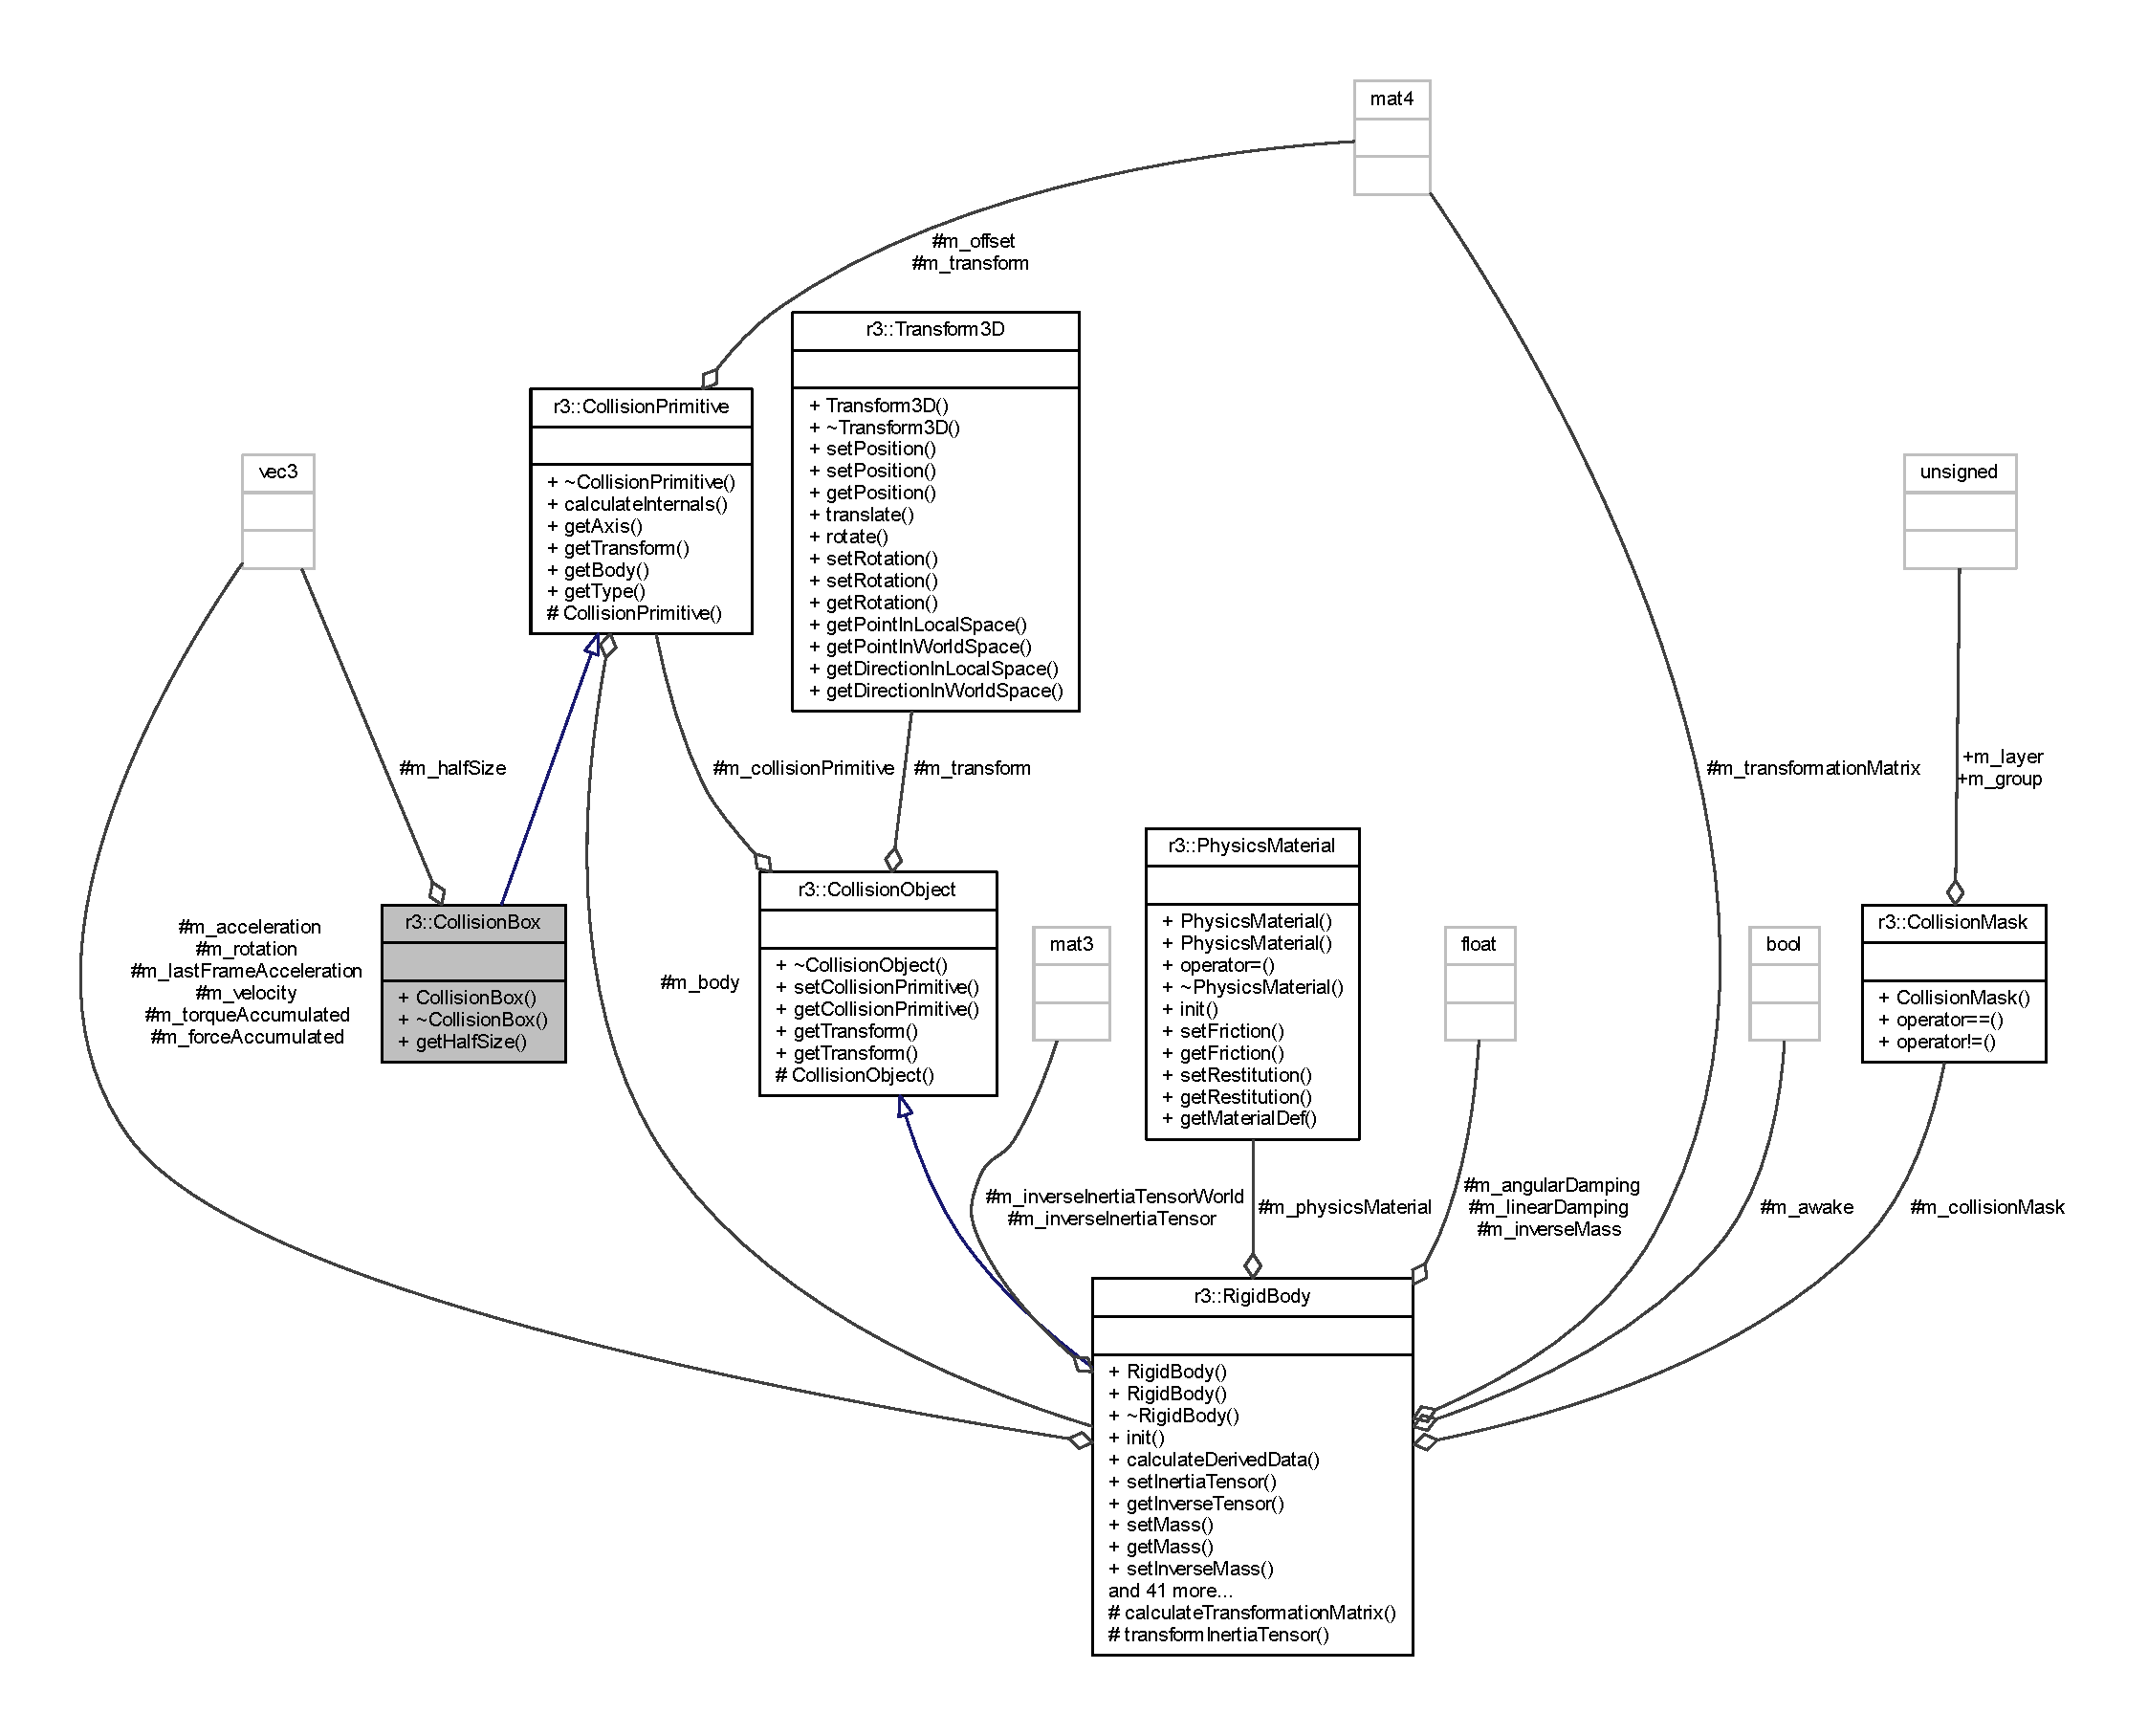
\includegraphics[width=350pt]{classr3_1_1_collision_box__coll__graph}
\end{center}
\end{figure}
\subsection*{Public Member Functions}
\begin{DoxyCompactItemize}
\item 
\mbox{\hyperlink{classr3_1_1_collision_box_ae8fd5f7a2fa804313c988f8b13866b91}{Collision\+Box}} (\mbox{\hyperlink{classr3_1_1_rigid_body}{Rigid\+Body}} $\ast$body, const glm\+::vec3 \&half\+Size, const glm\+::mat4 \&offset=glm\+::mat4(1))
\item 
\mbox{\hyperlink{classr3_1_1_collision_box_aab1d8f1b7999c61cff10b631305cc4f3}{$\sim$\+Collision\+Box}} ()
\item 
glm\+::vec3 \mbox{\hyperlink{classr3_1_1_collision_box_a6d35bfc27fd291409cb5e90ae2464179}{get\+Half\+Size}} () const
\end{DoxyCompactItemize}
\subsection*{Protected Attributes}
\begin{DoxyCompactItemize}
\item 
glm\+::vec3 \mbox{\hyperlink{classr3_1_1_collision_box_a91a3eaa48b16d7b0ca52ebadf4830bc8}{m\+\_\+half\+Size}}
\end{DoxyCompactItemize}
\subsection*{Additional Inherited Members}


\subsection{Constructor \& Destructor Documentation}
\mbox{\Hypertarget{classr3_1_1_collision_box_ae8fd5f7a2fa804313c988f8b13866b91}\label{classr3_1_1_collision_box_ae8fd5f7a2fa804313c988f8b13866b91}} 
\index{r3\+::\+Collision\+Box@{r3\+::\+Collision\+Box}!Collision\+Box@{Collision\+Box}}
\index{Collision\+Box@{Collision\+Box}!r3\+::\+Collision\+Box@{r3\+::\+Collision\+Box}}
\subsubsection{\texorpdfstring{Collision\+Box()}{CollisionBox()}}
{\footnotesize\ttfamily r3\+::\+Collision\+Box\+::\+Collision\+Box (\begin{DoxyParamCaption}\item[{\mbox{\hyperlink{classr3_1_1_rigid_body}{Rigid\+Body}} $\ast$}]{body,  }\item[{const glm\+::vec3 \&}]{half\+Size,  }\item[{const glm\+::mat4 \&}]{offset = {\ttfamily glm\+:\+:mat4(1)} }\end{DoxyParamCaption})\hspace{0.3cm}{\ttfamily [explicit]}}

\mbox{\Hypertarget{classr3_1_1_collision_box_aab1d8f1b7999c61cff10b631305cc4f3}\label{classr3_1_1_collision_box_aab1d8f1b7999c61cff10b631305cc4f3}} 
\index{r3\+::\+Collision\+Box@{r3\+::\+Collision\+Box}!````~Collision\+Box@{$\sim$\+Collision\+Box}}
\index{````~Collision\+Box@{$\sim$\+Collision\+Box}!r3\+::\+Collision\+Box@{r3\+::\+Collision\+Box}}
\subsubsection{\texorpdfstring{$\sim$\+Collision\+Box()}{~CollisionBox()}}
{\footnotesize\ttfamily r3\+::\+Collision\+Box\+::$\sim$\+Collision\+Box (\begin{DoxyParamCaption}{ }\end{DoxyParamCaption})\hspace{0.3cm}{\ttfamily [default]}}



\subsection{Member Function Documentation}
\mbox{\Hypertarget{classr3_1_1_collision_box_a6d35bfc27fd291409cb5e90ae2464179}\label{classr3_1_1_collision_box_a6d35bfc27fd291409cb5e90ae2464179}} 
\index{r3\+::\+Collision\+Box@{r3\+::\+Collision\+Box}!get\+Half\+Size@{get\+Half\+Size}}
\index{get\+Half\+Size@{get\+Half\+Size}!r3\+::\+Collision\+Box@{r3\+::\+Collision\+Box}}
\subsubsection{\texorpdfstring{get\+Half\+Size()}{getHalfSize()}}
{\footnotesize\ttfamily glm\+::vec3 r3\+::\+Collision\+Box\+::get\+Half\+Size (\begin{DoxyParamCaption}{ }\end{DoxyParamCaption}) const}



\subsection{Member Data Documentation}
\mbox{\Hypertarget{classr3_1_1_collision_box_a91a3eaa48b16d7b0ca52ebadf4830bc8}\label{classr3_1_1_collision_box_a91a3eaa48b16d7b0ca52ebadf4830bc8}} 
\index{r3\+::\+Collision\+Box@{r3\+::\+Collision\+Box}!m\+\_\+half\+Size@{m\+\_\+half\+Size}}
\index{m\+\_\+half\+Size@{m\+\_\+half\+Size}!r3\+::\+Collision\+Box@{r3\+::\+Collision\+Box}}
\subsubsection{\texorpdfstring{m\+\_\+half\+Size}{m\_halfSize}}
{\footnotesize\ttfamily glm\+::vec3 r3\+::\+Collision\+Box\+::m\+\_\+half\+Size\hspace{0.3cm}{\ttfamily [protected]}}



The documentation for this class was generated from the following files\+:\begin{DoxyCompactItemize}
\item 
D\+:/\+Job/\+Forschungsmaster/\+Projekte/\+Simulation\+Visualization/\+Rumble3\+D/\+Rumble3\+D/include/\+R3\+D/\+Rigid\+Body\+Engine/\mbox{\hyperlink{_collision_box_8h}{Collision\+Box.\+h}}\item 
D\+:/\+Job/\+Forschungsmaster/\+Projekte/\+Simulation\+Visualization/\+Rumble3\+D/\+Rumble3\+D/src/\+Rigid\+Body\+Engine/\mbox{\hyperlink{_collision_box_8cpp}{Collision\+Box.\+cpp}}\end{DoxyCompactItemize}

\hypertarget{classr3_1_1_collision_data}{}\section{r3\+:\+:Collision\+Data Class Reference}
\label{classr3_1_1_collision_data}\index{r3\+::\+Collision\+Data@{r3\+::\+Collision\+Data}}


{\ttfamily \#include $<$Collision\+Data.\+h$>$}



Collaboration diagram for r3\+:\+:Collision\+Data\+:\nopagebreak
\begin{figure}[H]
\begin{center}
\leavevmode
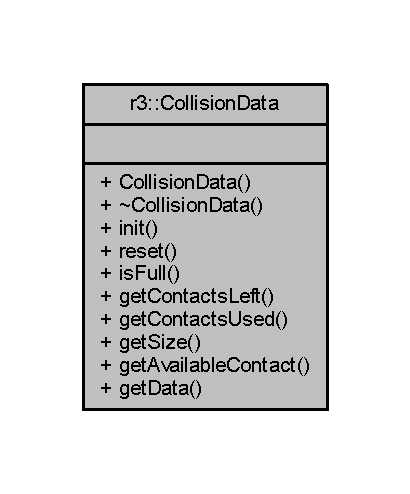
\includegraphics[width=197pt]{classr3_1_1_collision_data__coll__graph}
\end{center}
\end{figure}
\subsection*{Public Member Functions}
\begin{DoxyCompactItemize}
\item 
\mbox{\hyperlink{classr3_1_1_collision_data_a439100db9ec5b734e2f0b778d2f97cce}{Collision\+Data}} (unsigned int contacts\+Max=1000, int iterations=0)
\item 
\mbox{\hyperlink{classr3_1_1_collision_data_a3fd93aed7add6b43bc6b3dca59d638f2}{$\sim$\+Collision\+Data}} ()
\item 
void \mbox{\hyperlink{classr3_1_1_collision_data_a2af69fd6da492254b1a134d4ef82efce}{init}} (int contacts\+Max, int iterations)
\item 
void \mbox{\hyperlink{classr3_1_1_collision_data_af74822ca6881f5ab54447a73ac26d7fd}{reset}} ()
\item 
bool \mbox{\hyperlink{classr3_1_1_collision_data_aebb099e77b79235942a9c0166eb66a78}{is\+Full}} () const
\item 
bool \mbox{\hyperlink{classr3_1_1_collision_data_a3b97a4828252625e891c939ad7ce0064}{is\+Empty}} () const
\item 
int \mbox{\hyperlink{classr3_1_1_collision_data_a13e8ade4bbbbc63a1437de9371fea879}{get\+Contacts\+Left}} () const
\item 
int \mbox{\hyperlink{classr3_1_1_collision_data_aaf0e65914133cd35cc32224df851561e}{get\+Contacts\+Used}} () const
\item 
int \mbox{\hyperlink{classr3_1_1_collision_data_ad0898e21e34b4558dbdd68dd115c49d8}{get\+Size}} () const
\item 
\mbox{\hyperlink{namespacer3_ab2016b3e3f743fb735afce242f0dc1eb}{real}} \mbox{\hyperlink{classr3_1_1_collision_data_ae610a57c20c504a7bacb4e35f89f530f}{get\+Friction}} () const
\item 
\mbox{\hyperlink{namespacer3_ab2016b3e3f743fb735afce242f0dc1eb}{real}} \mbox{\hyperlink{classr3_1_1_collision_data_a4fa1a70757353fe8ae2facc3762f5b2b}{get\+Restitution}} () const
\item 
\mbox{\hyperlink{classr3_1_1_contact}{Contact}} $\ast$ \mbox{\hyperlink{classr3_1_1_collision_data_ad0e0b85004905b48a8faf7be34bdf305}{get\+Available\+Contact}} ()
\item 
std\+::vector$<$ \mbox{\hyperlink{classr3_1_1_contact}{Contact}} $>$ \& \mbox{\hyperlink{classr3_1_1_collision_data_acb1bb23e8d0f37f0ebc39e8f7642419f}{get\+Data}} ()
\item 
const std\+::vector$<$ \mbox{\hyperlink{classr3_1_1_contact}{Contact}} $>$ \& \mbox{\hyperlink{classr3_1_1_collision_data_ab31745ebb708c1d04e22bcfb385e663f}{get\+Data}} () const
\item 
void \mbox{\hyperlink{classr3_1_1_collision_data_a7a8dcf7d0b2cdd99d9c96dabc2a4fbc9}{prepare\+Contacts}} (\mbox{\hyperlink{namespacer3_ab2016b3e3f743fb735afce242f0dc1eb}{real}} time\+Delta)
\end{DoxyCompactItemize}


\subsection{Constructor \& Destructor Documentation}
\mbox{\Hypertarget{classr3_1_1_collision_data_a439100db9ec5b734e2f0b778d2f97cce}\label{classr3_1_1_collision_data_a439100db9ec5b734e2f0b778d2f97cce}} 
\index{r3\+::\+Collision\+Data@{r3\+::\+Collision\+Data}!Collision\+Data@{Collision\+Data}}
\index{Collision\+Data@{Collision\+Data}!r3\+::\+Collision\+Data@{r3\+::\+Collision\+Data}}
\subsubsection{\texorpdfstring{Collision\+Data()}{CollisionData()}}
{\footnotesize\ttfamily r3\+::\+Collision\+Data\+::\+Collision\+Data (\begin{DoxyParamCaption}\item[{unsigned int}]{contacts\+Max = {\ttfamily 1000},  }\item[{int}]{iterations = {\ttfamily 0} }\end{DoxyParamCaption})\hspace{0.3cm}{\ttfamily [explicit]}}

\mbox{\Hypertarget{classr3_1_1_collision_data_a3fd93aed7add6b43bc6b3dca59d638f2}\label{classr3_1_1_collision_data_a3fd93aed7add6b43bc6b3dca59d638f2}} 
\index{r3\+::\+Collision\+Data@{r3\+::\+Collision\+Data}!````~Collision\+Data@{$\sim$\+Collision\+Data}}
\index{````~Collision\+Data@{$\sim$\+Collision\+Data}!r3\+::\+Collision\+Data@{r3\+::\+Collision\+Data}}
\subsubsection{\texorpdfstring{$\sim$\+Collision\+Data()}{~CollisionData()}}
{\footnotesize\ttfamily r3\+::\+Collision\+Data\+::$\sim$\+Collision\+Data (\begin{DoxyParamCaption}{ }\end{DoxyParamCaption})\hspace{0.3cm}{\ttfamily [default]}}



\subsection{Member Function Documentation}
\mbox{\Hypertarget{classr3_1_1_collision_data_ad0e0b85004905b48a8faf7be34bdf305}\label{classr3_1_1_collision_data_ad0e0b85004905b48a8faf7be34bdf305}} 
\index{r3\+::\+Collision\+Data@{r3\+::\+Collision\+Data}!get\+Available\+Contact@{get\+Available\+Contact}}
\index{get\+Available\+Contact@{get\+Available\+Contact}!r3\+::\+Collision\+Data@{r3\+::\+Collision\+Data}}
\subsubsection{\texorpdfstring{get\+Available\+Contact()}{getAvailableContact()}}
{\footnotesize\ttfamily \mbox{\hyperlink{classr3_1_1_contact}{Contact}} $\ast$ r3\+::\+Collision\+Data\+::get\+Available\+Contact (\begin{DoxyParamCaption}{ }\end{DoxyParamCaption})}

Get the next available contact. Automatically uses it! \begin{DoxyReturn}{Returns}
nullptr if all contacts are used, a available contact otherwise. 
\end{DoxyReturn}
\mbox{\Hypertarget{classr3_1_1_collision_data_a13e8ade4bbbbc63a1437de9371fea879}\label{classr3_1_1_collision_data_a13e8ade4bbbbc63a1437de9371fea879}} 
\index{r3\+::\+Collision\+Data@{r3\+::\+Collision\+Data}!get\+Contacts\+Left@{get\+Contacts\+Left}}
\index{get\+Contacts\+Left@{get\+Contacts\+Left}!r3\+::\+Collision\+Data@{r3\+::\+Collision\+Data}}
\subsubsection{\texorpdfstring{get\+Contacts\+Left()}{getContactsLeft()}}
{\footnotesize\ttfamily int r3\+::\+Collision\+Data\+::get\+Contacts\+Left (\begin{DoxyParamCaption}{ }\end{DoxyParamCaption}) const}

Check how many contacts can still be inserted. \mbox{\Hypertarget{classr3_1_1_collision_data_aaf0e65914133cd35cc32224df851561e}\label{classr3_1_1_collision_data_aaf0e65914133cd35cc32224df851561e}} 
\index{r3\+::\+Collision\+Data@{r3\+::\+Collision\+Data}!get\+Contacts\+Used@{get\+Contacts\+Used}}
\index{get\+Contacts\+Used@{get\+Contacts\+Used}!r3\+::\+Collision\+Data@{r3\+::\+Collision\+Data}}
\subsubsection{\texorpdfstring{get\+Contacts\+Used()}{getContactsUsed()}}
{\footnotesize\ttfamily int r3\+::\+Collision\+Data\+::get\+Contacts\+Used (\begin{DoxyParamCaption}{ }\end{DoxyParamCaption}) const}

Check how many contacts have been inserted. \mbox{\Hypertarget{classr3_1_1_collision_data_acb1bb23e8d0f37f0ebc39e8f7642419f}\label{classr3_1_1_collision_data_acb1bb23e8d0f37f0ebc39e8f7642419f}} 
\index{r3\+::\+Collision\+Data@{r3\+::\+Collision\+Data}!get\+Data@{get\+Data}}
\index{get\+Data@{get\+Data}!r3\+::\+Collision\+Data@{r3\+::\+Collision\+Data}}
\subsubsection{\texorpdfstring{get\+Data()}{getData()}\hspace{0.1cm}{\footnotesize\ttfamily [1/2]}}
{\footnotesize\ttfamily std\+::vector$<$ \mbox{\hyperlink{classr3_1_1_contact}{Contact}} $>$ \& r3\+::\+Collision\+Data\+::get\+Data (\begin{DoxyParamCaption}{ }\end{DoxyParamCaption})}

Get all contacts (only valid to a certain position) \mbox{\Hypertarget{classr3_1_1_collision_data_ab31745ebb708c1d04e22bcfb385e663f}\label{classr3_1_1_collision_data_ab31745ebb708c1d04e22bcfb385e663f}} 
\index{r3\+::\+Collision\+Data@{r3\+::\+Collision\+Data}!get\+Data@{get\+Data}}
\index{get\+Data@{get\+Data}!r3\+::\+Collision\+Data@{r3\+::\+Collision\+Data}}
\subsubsection{\texorpdfstring{get\+Data()}{getData()}\hspace{0.1cm}{\footnotesize\ttfamily [2/2]}}
{\footnotesize\ttfamily const std\+::vector$<$ \mbox{\hyperlink{classr3_1_1_contact}{Contact}} $>$ \& r3\+::\+Collision\+Data\+::get\+Data (\begin{DoxyParamCaption}{ }\end{DoxyParamCaption}) const}

Get all contacts (only valid to a certain position) \mbox{\Hypertarget{classr3_1_1_collision_data_ae610a57c20c504a7bacb4e35f89f530f}\label{classr3_1_1_collision_data_ae610a57c20c504a7bacb4e35f89f530f}} 
\index{r3\+::\+Collision\+Data@{r3\+::\+Collision\+Data}!get\+Friction@{get\+Friction}}
\index{get\+Friction@{get\+Friction}!r3\+::\+Collision\+Data@{r3\+::\+Collision\+Data}}
\subsubsection{\texorpdfstring{get\+Friction()}{getFriction()}}
{\footnotesize\ttfamily \mbox{\hyperlink{namespacer3_ab2016b3e3f743fb735afce242f0dc1eb}{real}} r3\+::\+Collision\+Data\+::get\+Friction (\begin{DoxyParamCaption}{ }\end{DoxyParamCaption}) const\hspace{0.3cm}{\ttfamily [inline]}}

\begin{DoxyRefDesc}{Todo}
\item[\mbox{\hyperlink{todo__todo000002}{Todo}}]use physic material in rigid body instead. \end{DoxyRefDesc}
\mbox{\Hypertarget{classr3_1_1_collision_data_a4fa1a70757353fe8ae2facc3762f5b2b}\label{classr3_1_1_collision_data_a4fa1a70757353fe8ae2facc3762f5b2b}} 
\index{r3\+::\+Collision\+Data@{r3\+::\+Collision\+Data}!get\+Restitution@{get\+Restitution}}
\index{get\+Restitution@{get\+Restitution}!r3\+::\+Collision\+Data@{r3\+::\+Collision\+Data}}
\subsubsection{\texorpdfstring{get\+Restitution()}{getRestitution()}}
{\footnotesize\ttfamily \mbox{\hyperlink{namespacer3_ab2016b3e3f743fb735afce242f0dc1eb}{real}} r3\+::\+Collision\+Data\+::get\+Restitution (\begin{DoxyParamCaption}{ }\end{DoxyParamCaption}) const\hspace{0.3cm}{\ttfamily [inline]}}

\begin{DoxyRefDesc}{Todo}
\item[\mbox{\hyperlink{todo__todo000003}{Todo}}]use physic material in rigid body instead. \end{DoxyRefDesc}
\mbox{\Hypertarget{classr3_1_1_collision_data_ad0898e21e34b4558dbdd68dd115c49d8}\label{classr3_1_1_collision_data_ad0898e21e34b4558dbdd68dd115c49d8}} 
\index{r3\+::\+Collision\+Data@{r3\+::\+Collision\+Data}!get\+Size@{get\+Size}}
\index{get\+Size@{get\+Size}!r3\+::\+Collision\+Data@{r3\+::\+Collision\+Data}}
\subsubsection{\texorpdfstring{get\+Size()}{getSize()}}
{\footnotesize\ttfamily int r3\+::\+Collision\+Data\+::get\+Size (\begin{DoxyParamCaption}{ }\end{DoxyParamCaption}) const}

Get the maximal number of contacts. \mbox{\Hypertarget{classr3_1_1_collision_data_a2af69fd6da492254b1a134d4ef82efce}\label{classr3_1_1_collision_data_a2af69fd6da492254b1a134d4ef82efce}} 
\index{r3\+::\+Collision\+Data@{r3\+::\+Collision\+Data}!init@{init}}
\index{init@{init}!r3\+::\+Collision\+Data@{r3\+::\+Collision\+Data}}
\subsubsection{\texorpdfstring{init()}{init()}}
{\footnotesize\ttfamily void r3\+::\+Collision\+Data\+::init (\begin{DoxyParamCaption}\item[{int}]{contacts\+Max,  }\item[{int}]{iterations }\end{DoxyParamCaption})}

\mbox{\Hypertarget{classr3_1_1_collision_data_a3b97a4828252625e891c939ad7ce0064}\label{classr3_1_1_collision_data_a3b97a4828252625e891c939ad7ce0064}} 
\index{r3\+::\+Collision\+Data@{r3\+::\+Collision\+Data}!is\+Empty@{is\+Empty}}
\index{is\+Empty@{is\+Empty}!r3\+::\+Collision\+Data@{r3\+::\+Collision\+Data}}
\subsubsection{\texorpdfstring{is\+Empty()}{isEmpty()}}
{\footnotesize\ttfamily bool r3\+::\+Collision\+Data\+::is\+Empty (\begin{DoxyParamCaption}{ }\end{DoxyParamCaption}) const}

Check if no contacts are used. \mbox{\Hypertarget{classr3_1_1_collision_data_aebb099e77b79235942a9c0166eb66a78}\label{classr3_1_1_collision_data_aebb099e77b79235942a9c0166eb66a78}} 
\index{r3\+::\+Collision\+Data@{r3\+::\+Collision\+Data}!is\+Full@{is\+Full}}
\index{is\+Full@{is\+Full}!r3\+::\+Collision\+Data@{r3\+::\+Collision\+Data}}
\subsubsection{\texorpdfstring{is\+Full()}{isFull()}}
{\footnotesize\ttfamily bool r3\+::\+Collision\+Data\+::is\+Full (\begin{DoxyParamCaption}{ }\end{DoxyParamCaption}) const}

Check if there is no more room for new contacts. \mbox{\Hypertarget{classr3_1_1_collision_data_a7a8dcf7d0b2cdd99d9c96dabc2a4fbc9}\label{classr3_1_1_collision_data_a7a8dcf7d0b2cdd99d9c96dabc2a4fbc9}} 
\index{r3\+::\+Collision\+Data@{r3\+::\+Collision\+Data}!prepare\+Contacts@{prepare\+Contacts}}
\index{prepare\+Contacts@{prepare\+Contacts}!r3\+::\+Collision\+Data@{r3\+::\+Collision\+Data}}
\subsubsection{\texorpdfstring{prepare\+Contacts()}{prepareContacts()}}
{\footnotesize\ttfamily void r3\+::\+Collision\+Data\+::prepare\+Contacts (\begin{DoxyParamCaption}\item[{\mbox{\hyperlink{namespacer3_ab2016b3e3f743fb735afce242f0dc1eb}{real}}}]{time\+Delta }\end{DoxyParamCaption})}

\mbox{\Hypertarget{classr3_1_1_collision_data_af74822ca6881f5ab54447a73ac26d7fd}\label{classr3_1_1_collision_data_af74822ca6881f5ab54447a73ac26d7fd}} 
\index{r3\+::\+Collision\+Data@{r3\+::\+Collision\+Data}!reset@{reset}}
\index{reset@{reset}!r3\+::\+Collision\+Data@{r3\+::\+Collision\+Data}}
\subsubsection{\texorpdfstring{reset()}{reset()}}
{\footnotesize\ttfamily void r3\+::\+Collision\+Data\+::reset (\begin{DoxyParamCaption}{ }\end{DoxyParamCaption})}



The documentation for this class was generated from the following files\+:\begin{DoxyCompactItemize}
\item 
D\+:/\+Library/\+Documents/\+Job/\+Forschungsmaster/\+Projekte/\+Simulation\+Visualization/\+Rumble3\+D/\+Rumble3\+D/include/\+R3\+D/\+Rigid\+Body\+Engine/\+Collision\+Detection/\mbox{\hyperlink{_collision_data_8h}{Collision\+Data.\+h}}\item 
D\+:/\+Library/\+Documents/\+Job/\+Forschungsmaster/\+Projekte/\+Simulation\+Visualization/\+Rumble3\+D/\+Rumble3\+D/src/\+Rigid\+Body\+Engine/\+Collision\+Detection/\mbox{\hyperlink{_collision_data_8cpp}{Collision\+Data.\+cpp}}\end{DoxyCompactItemize}

\hypertarget{classr3_1_1_collision_data_old}{}\section{r3\+:\+:Collision\+Data\+Old Class Reference}
\label{classr3_1_1_collision_data_old}\index{r3\+::\+Collision\+Data\+Old@{r3\+::\+Collision\+Data\+Old}}


{\ttfamily \#include $<$Collision\+Data\+Old.\+h$>$}



Collaboration diagram for r3\+:\+:Collision\+Data\+Old\+:\nopagebreak
\begin{figure}[H]
\begin{center}
\leavevmode
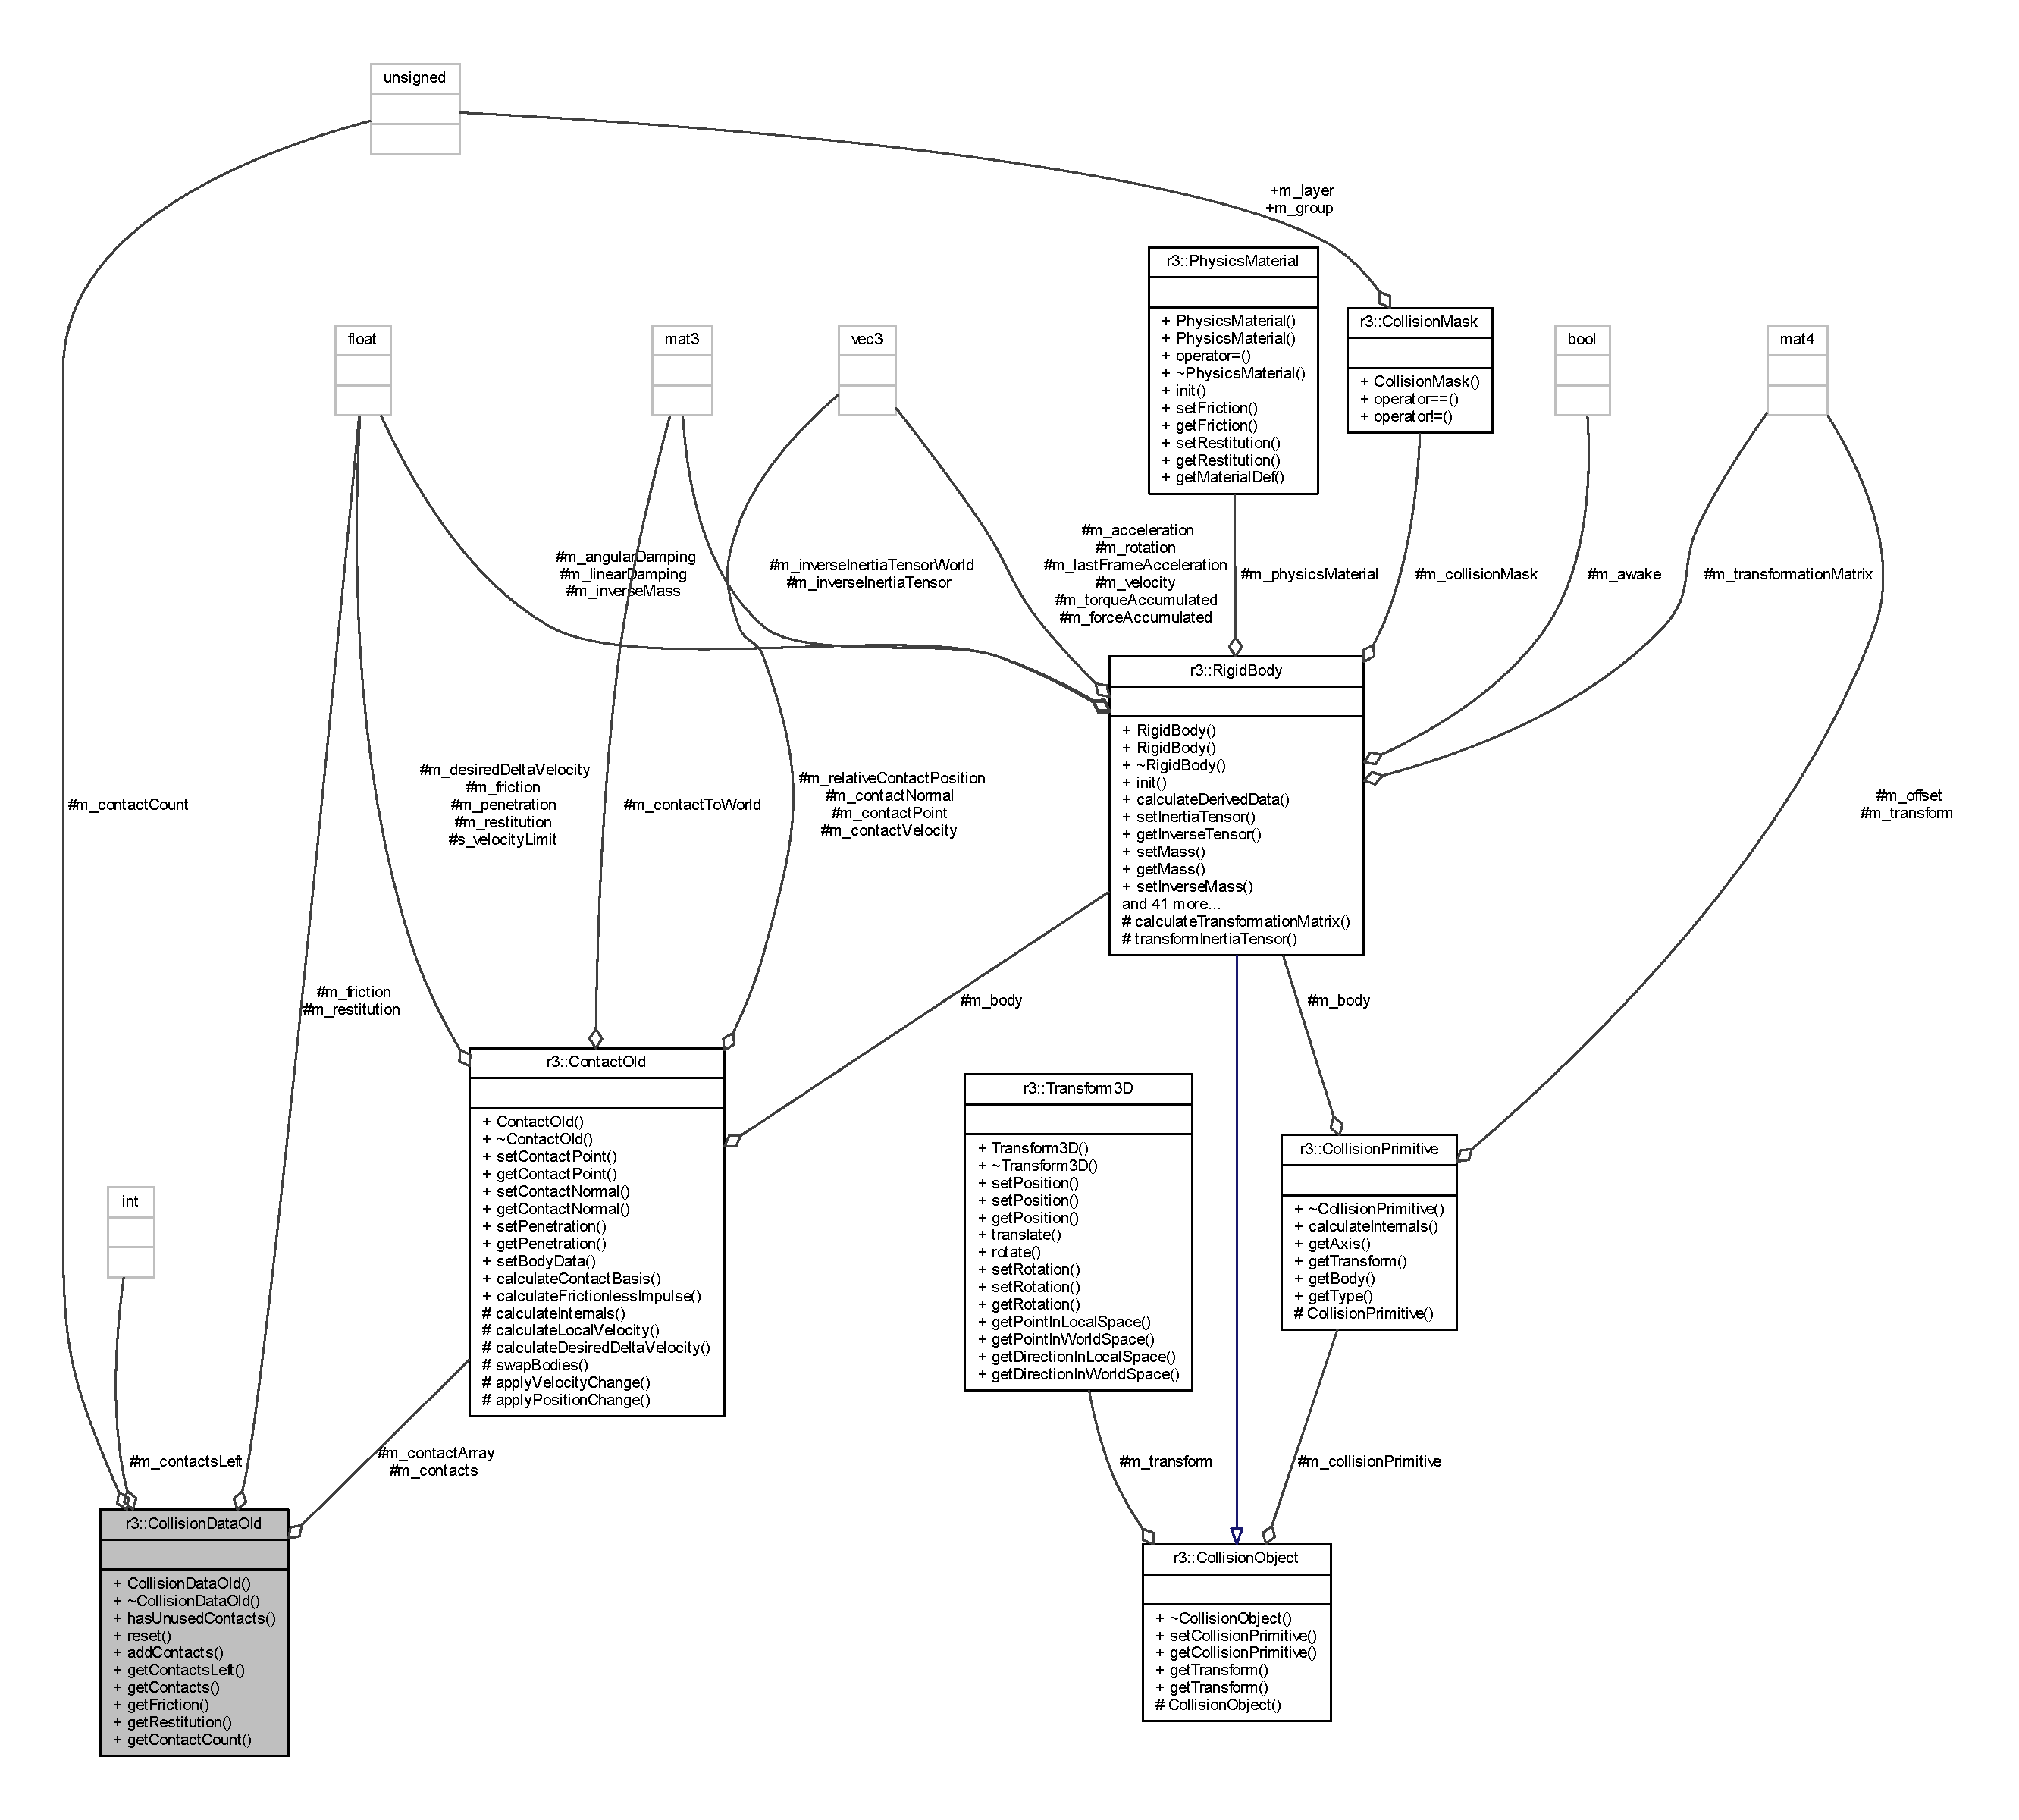
\includegraphics[width=350pt]{classr3_1_1_collision_data_old__coll__graph}
\end{center}
\end{figure}
\subsection*{Public Member Functions}
\begin{DoxyCompactItemize}
\item 
\mbox{\hyperlink{classr3_1_1_collision_data_old_a707e8f38c09df2da7d7ae6a52e418379}{Collision\+Data\+Old}} ()
\item 
\mbox{\hyperlink{classr3_1_1_collision_data_old_a7afc80cbab2af8ed71fcce5064dcf518}{$\sim$\+Collision\+Data\+Old}} ()
\item 
bool \mbox{\hyperlink{classr3_1_1_collision_data_old_a84bd3d8cbf7b3b2f26f31c8a1e1d6b0e}{has\+Unused\+Contacts}} () const
\item 
void \mbox{\hyperlink{classr3_1_1_collision_data_old_a30b66c4a32bd509ee6cd72d7a3e41ef0}{reset}} (unsigned max\+Contacts)
\item 
void \mbox{\hyperlink{classr3_1_1_collision_data_old_ae2b77d8254b53bfa4640ea3ad833370c}{add\+Contacts}} (unsigned count)
\item 
int \mbox{\hyperlink{classr3_1_1_collision_data_old_a78d2328616c76e498822df4cb0690832}{get\+Contacts\+Left}} () const
\item 
\mbox{\hyperlink{classr3_1_1_contact_old}{Contact\+Old}} $\ast$ \mbox{\hyperlink{classr3_1_1_collision_data_old_a5df14bfb6d789df7663b64306756eb96}{get\+Contacts}} () const
\item 
\mbox{\hyperlink{namespacer3_ab2016b3e3f743fb735afce242f0dc1eb}{real}} \mbox{\hyperlink{classr3_1_1_collision_data_old_af6d03fd7fe8df176e9e8860e7d1d4119}{get\+Friction}} () const
\item 
\mbox{\hyperlink{namespacer3_ab2016b3e3f743fb735afce242f0dc1eb}{real}} \mbox{\hyperlink{classr3_1_1_collision_data_old_a3546df5d0d82e690c12f0899bc683d35}{get\+Restitution}} () const
\item 
int \mbox{\hyperlink{classr3_1_1_collision_data_old_a7bdf6b83595d88f4e716bf74a1a1ab3c}{get\+Contact\+Count}} () const
\end{DoxyCompactItemize}
\subsection*{Protected Attributes}
\begin{DoxyCompactItemize}
\item 
\mbox{\hyperlink{classr3_1_1_contact_old}{Contact\+Old}} $\ast$ \mbox{\hyperlink{classr3_1_1_collision_data_old_a2100ba5e8b3f49926d09b2ad5ca547f1}{m\+\_\+contact\+Array}} \{\}
\item 
\mbox{\hyperlink{classr3_1_1_contact_old}{Contact\+Old}} $\ast$ \mbox{\hyperlink{classr3_1_1_collision_data_old_ac0396f857d87d2a209250c9742eb7fb3}{m\+\_\+contacts}} \{\}
\item 
int \mbox{\hyperlink{classr3_1_1_collision_data_old_ad18fd7d0136d1e6d80c7c5340652a08d}{m\+\_\+contacts\+Left}} \{\}
\item 
unsigned \mbox{\hyperlink{classr3_1_1_collision_data_old_af89be6ec7df393c62d8cfa27bbf27d5f}{m\+\_\+contact\+Count}} \{\}
\item 
\mbox{\hyperlink{namespacer3_ab2016b3e3f743fb735afce242f0dc1eb}{real}} \mbox{\hyperlink{classr3_1_1_collision_data_old_a598bcf57a27bd4ed84eab8f64b334c12}{m\+\_\+friction}} = 0.\+5f
\item 
\mbox{\hyperlink{namespacer3_ab2016b3e3f743fb735afce242f0dc1eb}{real}} \mbox{\hyperlink{classr3_1_1_collision_data_old_ae4fb8abfc80fdf2637e89bd2ef621aac}{m\+\_\+restitution}} = 0.\+5f
\end{DoxyCompactItemize}


\subsection{Constructor \& Destructor Documentation}
\mbox{\Hypertarget{classr3_1_1_collision_data_old_a707e8f38c09df2da7d7ae6a52e418379}\label{classr3_1_1_collision_data_old_a707e8f38c09df2da7d7ae6a52e418379}} 
\index{r3\+::\+Collision\+Data\+Old@{r3\+::\+Collision\+Data\+Old}!Collision\+Data\+Old@{Collision\+Data\+Old}}
\index{Collision\+Data\+Old@{Collision\+Data\+Old}!r3\+::\+Collision\+Data\+Old@{r3\+::\+Collision\+Data\+Old}}
\subsubsection{\texorpdfstring{Collision\+Data\+Old()}{CollisionDataOld()}}
{\footnotesize\ttfamily r3\+::\+Collision\+Data\+Old\+::\+Collision\+Data\+Old (\begin{DoxyParamCaption}{ }\end{DoxyParamCaption})\hspace{0.3cm}{\ttfamily [explicit]}, {\ttfamily [default]}}

\mbox{\Hypertarget{classr3_1_1_collision_data_old_a7afc80cbab2af8ed71fcce5064dcf518}\label{classr3_1_1_collision_data_old_a7afc80cbab2af8ed71fcce5064dcf518}} 
\index{r3\+::\+Collision\+Data\+Old@{r3\+::\+Collision\+Data\+Old}!````~Collision\+Data\+Old@{$\sim$\+Collision\+Data\+Old}}
\index{````~Collision\+Data\+Old@{$\sim$\+Collision\+Data\+Old}!r3\+::\+Collision\+Data\+Old@{r3\+::\+Collision\+Data\+Old}}
\subsubsection{\texorpdfstring{$\sim$\+Collision\+Data\+Old()}{~CollisionDataOld()}}
{\footnotesize\ttfamily r3\+::\+Collision\+Data\+Old\+::$\sim$\+Collision\+Data\+Old (\begin{DoxyParamCaption}{ }\end{DoxyParamCaption})\hspace{0.3cm}{\ttfamily [default]}}



\subsection{Member Function Documentation}
\mbox{\Hypertarget{classr3_1_1_collision_data_old_ae2b77d8254b53bfa4640ea3ad833370c}\label{classr3_1_1_collision_data_old_ae2b77d8254b53bfa4640ea3ad833370c}} 
\index{r3\+::\+Collision\+Data\+Old@{r3\+::\+Collision\+Data\+Old}!add\+Contacts@{add\+Contacts}}
\index{add\+Contacts@{add\+Contacts}!r3\+::\+Collision\+Data\+Old@{r3\+::\+Collision\+Data\+Old}}
\subsubsection{\texorpdfstring{add\+Contacts()}{addContacts()}}
{\footnotesize\ttfamily void r3\+::\+Collision\+Data\+Old\+::add\+Contacts (\begin{DoxyParamCaption}\item[{unsigned}]{count }\end{DoxyParamCaption})}

\mbox{\Hypertarget{classr3_1_1_collision_data_old_a7bdf6b83595d88f4e716bf74a1a1ab3c}\label{classr3_1_1_collision_data_old_a7bdf6b83595d88f4e716bf74a1a1ab3c}} 
\index{r3\+::\+Collision\+Data\+Old@{r3\+::\+Collision\+Data\+Old}!get\+Contact\+Count@{get\+Contact\+Count}}
\index{get\+Contact\+Count@{get\+Contact\+Count}!r3\+::\+Collision\+Data\+Old@{r3\+::\+Collision\+Data\+Old}}
\subsubsection{\texorpdfstring{get\+Contact\+Count()}{getContactCount()}}
{\footnotesize\ttfamily int r3\+::\+Collision\+Data\+Old\+::get\+Contact\+Count (\begin{DoxyParamCaption}{ }\end{DoxyParamCaption}) const}

\mbox{\Hypertarget{classr3_1_1_collision_data_old_a5df14bfb6d789df7663b64306756eb96}\label{classr3_1_1_collision_data_old_a5df14bfb6d789df7663b64306756eb96}} 
\index{r3\+::\+Collision\+Data\+Old@{r3\+::\+Collision\+Data\+Old}!get\+Contacts@{get\+Contacts}}
\index{get\+Contacts@{get\+Contacts}!r3\+::\+Collision\+Data\+Old@{r3\+::\+Collision\+Data\+Old}}
\subsubsection{\texorpdfstring{get\+Contacts()}{getContacts()}}
{\footnotesize\ttfamily \mbox{\hyperlink{classr3_1_1_contact_old}{Contact\+Old}} $\ast$ r3\+::\+Collision\+Data\+Old\+::get\+Contacts (\begin{DoxyParamCaption}{ }\end{DoxyParamCaption}) const}

\mbox{\Hypertarget{classr3_1_1_collision_data_old_a78d2328616c76e498822df4cb0690832}\label{classr3_1_1_collision_data_old_a78d2328616c76e498822df4cb0690832}} 
\index{r3\+::\+Collision\+Data\+Old@{r3\+::\+Collision\+Data\+Old}!get\+Contacts\+Left@{get\+Contacts\+Left}}
\index{get\+Contacts\+Left@{get\+Contacts\+Left}!r3\+::\+Collision\+Data\+Old@{r3\+::\+Collision\+Data\+Old}}
\subsubsection{\texorpdfstring{get\+Contacts\+Left()}{getContactsLeft()}}
{\footnotesize\ttfamily int r3\+::\+Collision\+Data\+Old\+::get\+Contacts\+Left (\begin{DoxyParamCaption}{ }\end{DoxyParamCaption}) const}

\mbox{\Hypertarget{classr3_1_1_collision_data_old_af6d03fd7fe8df176e9e8860e7d1d4119}\label{classr3_1_1_collision_data_old_af6d03fd7fe8df176e9e8860e7d1d4119}} 
\index{r3\+::\+Collision\+Data\+Old@{r3\+::\+Collision\+Data\+Old}!get\+Friction@{get\+Friction}}
\index{get\+Friction@{get\+Friction}!r3\+::\+Collision\+Data\+Old@{r3\+::\+Collision\+Data\+Old}}
\subsubsection{\texorpdfstring{get\+Friction()}{getFriction()}}
{\footnotesize\ttfamily \mbox{\hyperlink{namespacer3_ab2016b3e3f743fb735afce242f0dc1eb}{real}} r3\+::\+Collision\+Data\+Old\+::get\+Friction (\begin{DoxyParamCaption}{ }\end{DoxyParamCaption}) const}

\mbox{\Hypertarget{classr3_1_1_collision_data_old_a3546df5d0d82e690c12f0899bc683d35}\label{classr3_1_1_collision_data_old_a3546df5d0d82e690c12f0899bc683d35}} 
\index{r3\+::\+Collision\+Data\+Old@{r3\+::\+Collision\+Data\+Old}!get\+Restitution@{get\+Restitution}}
\index{get\+Restitution@{get\+Restitution}!r3\+::\+Collision\+Data\+Old@{r3\+::\+Collision\+Data\+Old}}
\subsubsection{\texorpdfstring{get\+Restitution()}{getRestitution()}}
{\footnotesize\ttfamily \mbox{\hyperlink{namespacer3_ab2016b3e3f743fb735afce242f0dc1eb}{real}} r3\+::\+Collision\+Data\+Old\+::get\+Restitution (\begin{DoxyParamCaption}{ }\end{DoxyParamCaption}) const}

\mbox{\Hypertarget{classr3_1_1_collision_data_old_a84bd3d8cbf7b3b2f26f31c8a1e1d6b0e}\label{classr3_1_1_collision_data_old_a84bd3d8cbf7b3b2f26f31c8a1e1d6b0e}} 
\index{r3\+::\+Collision\+Data\+Old@{r3\+::\+Collision\+Data\+Old}!has\+Unused\+Contacts@{has\+Unused\+Contacts}}
\index{has\+Unused\+Contacts@{has\+Unused\+Contacts}!r3\+::\+Collision\+Data\+Old@{r3\+::\+Collision\+Data\+Old}}
\subsubsection{\texorpdfstring{has\+Unused\+Contacts()}{hasUnusedContacts()}}
{\footnotesize\ttfamily bool r3\+::\+Collision\+Data\+Old\+::has\+Unused\+Contacts (\begin{DoxyParamCaption}{ }\end{DoxyParamCaption}) const}

\mbox{\Hypertarget{classr3_1_1_collision_data_old_a30b66c4a32bd509ee6cd72d7a3e41ef0}\label{classr3_1_1_collision_data_old_a30b66c4a32bd509ee6cd72d7a3e41ef0}} 
\index{r3\+::\+Collision\+Data\+Old@{r3\+::\+Collision\+Data\+Old}!reset@{reset}}
\index{reset@{reset}!r3\+::\+Collision\+Data\+Old@{r3\+::\+Collision\+Data\+Old}}
\subsubsection{\texorpdfstring{reset()}{reset()}}
{\footnotesize\ttfamily void r3\+::\+Collision\+Data\+Old\+::reset (\begin{DoxyParamCaption}\item[{unsigned}]{max\+Contacts }\end{DoxyParamCaption})}



\subsection{Member Data Documentation}
\mbox{\Hypertarget{classr3_1_1_collision_data_old_a2100ba5e8b3f49926d09b2ad5ca547f1}\label{classr3_1_1_collision_data_old_a2100ba5e8b3f49926d09b2ad5ca547f1}} 
\index{r3\+::\+Collision\+Data\+Old@{r3\+::\+Collision\+Data\+Old}!m\+\_\+contact\+Array@{m\+\_\+contact\+Array}}
\index{m\+\_\+contact\+Array@{m\+\_\+contact\+Array}!r3\+::\+Collision\+Data\+Old@{r3\+::\+Collision\+Data\+Old}}
\subsubsection{\texorpdfstring{m\+\_\+contact\+Array}{m\_contactArray}}
{\footnotesize\ttfamily \mbox{\hyperlink{classr3_1_1_contact_old}{Contact\+Old}}$\ast$ r3\+::\+Collision\+Data\+Old\+::m\+\_\+contact\+Array \{\}\hspace{0.3cm}{\ttfamily [protected]}}

\mbox{\Hypertarget{classr3_1_1_collision_data_old_af89be6ec7df393c62d8cfa27bbf27d5f}\label{classr3_1_1_collision_data_old_af89be6ec7df393c62d8cfa27bbf27d5f}} 
\index{r3\+::\+Collision\+Data\+Old@{r3\+::\+Collision\+Data\+Old}!m\+\_\+contact\+Count@{m\+\_\+contact\+Count}}
\index{m\+\_\+contact\+Count@{m\+\_\+contact\+Count}!r3\+::\+Collision\+Data\+Old@{r3\+::\+Collision\+Data\+Old}}
\subsubsection{\texorpdfstring{m\+\_\+contact\+Count}{m\_contactCount}}
{\footnotesize\ttfamily unsigned r3\+::\+Collision\+Data\+Old\+::m\+\_\+contact\+Count \{\}\hspace{0.3cm}{\ttfamily [protected]}}

\mbox{\Hypertarget{classr3_1_1_collision_data_old_ac0396f857d87d2a209250c9742eb7fb3}\label{classr3_1_1_collision_data_old_ac0396f857d87d2a209250c9742eb7fb3}} 
\index{r3\+::\+Collision\+Data\+Old@{r3\+::\+Collision\+Data\+Old}!m\+\_\+contacts@{m\+\_\+contacts}}
\index{m\+\_\+contacts@{m\+\_\+contacts}!r3\+::\+Collision\+Data\+Old@{r3\+::\+Collision\+Data\+Old}}
\subsubsection{\texorpdfstring{m\+\_\+contacts}{m\_contacts}}
{\footnotesize\ttfamily \mbox{\hyperlink{classr3_1_1_contact_old}{Contact\+Old}}$\ast$ r3\+::\+Collision\+Data\+Old\+::m\+\_\+contacts \{\}\hspace{0.3cm}{\ttfamily [protected]}}

\mbox{\Hypertarget{classr3_1_1_collision_data_old_ad18fd7d0136d1e6d80c7c5340652a08d}\label{classr3_1_1_collision_data_old_ad18fd7d0136d1e6d80c7c5340652a08d}} 
\index{r3\+::\+Collision\+Data\+Old@{r3\+::\+Collision\+Data\+Old}!m\+\_\+contacts\+Left@{m\+\_\+contacts\+Left}}
\index{m\+\_\+contacts\+Left@{m\+\_\+contacts\+Left}!r3\+::\+Collision\+Data\+Old@{r3\+::\+Collision\+Data\+Old}}
\subsubsection{\texorpdfstring{m\+\_\+contacts\+Left}{m\_contactsLeft}}
{\footnotesize\ttfamily int r3\+::\+Collision\+Data\+Old\+::m\+\_\+contacts\+Left \{\}\hspace{0.3cm}{\ttfamily [protected]}}

\mbox{\Hypertarget{classr3_1_1_collision_data_old_a598bcf57a27bd4ed84eab8f64b334c12}\label{classr3_1_1_collision_data_old_a598bcf57a27bd4ed84eab8f64b334c12}} 
\index{r3\+::\+Collision\+Data\+Old@{r3\+::\+Collision\+Data\+Old}!m\+\_\+friction@{m\+\_\+friction}}
\index{m\+\_\+friction@{m\+\_\+friction}!r3\+::\+Collision\+Data\+Old@{r3\+::\+Collision\+Data\+Old}}
\subsubsection{\texorpdfstring{m\+\_\+friction}{m\_friction}}
{\footnotesize\ttfamily \mbox{\hyperlink{namespacer3_ab2016b3e3f743fb735afce242f0dc1eb}{real}} r3\+::\+Collision\+Data\+Old\+::m\+\_\+friction = 0.\+5f\hspace{0.3cm}{\ttfamily [protected]}}

\mbox{\Hypertarget{classr3_1_1_collision_data_old_ae4fb8abfc80fdf2637e89bd2ef621aac}\label{classr3_1_1_collision_data_old_ae4fb8abfc80fdf2637e89bd2ef621aac}} 
\index{r3\+::\+Collision\+Data\+Old@{r3\+::\+Collision\+Data\+Old}!m\+\_\+restitution@{m\+\_\+restitution}}
\index{m\+\_\+restitution@{m\+\_\+restitution}!r3\+::\+Collision\+Data\+Old@{r3\+::\+Collision\+Data\+Old}}
\subsubsection{\texorpdfstring{m\+\_\+restitution}{m\_restitution}}
{\footnotesize\ttfamily \mbox{\hyperlink{namespacer3_ab2016b3e3f743fb735afce242f0dc1eb}{real}} r3\+::\+Collision\+Data\+Old\+::m\+\_\+restitution = 0.\+5f\hspace{0.3cm}{\ttfamily [protected]}}



The documentation for this class was generated from the following files\+:\begin{DoxyCompactItemize}
\item 
D\+:/\+Job/\+Forschungsmaster/\+Projekte/\+Simulation\+Visualization/\+Rumble3\+D/\+Rumble3\+D/include/\+R3\+D/\+Rigid\+Body\+Engine/\mbox{\hyperlink{_collision_data_old_8h}{Collision\+Data\+Old.\+h}}\item 
D\+:/\+Job/\+Forschungsmaster/\+Projekte/\+Simulation\+Visualization/\+Rumble3\+D/\+Rumble3\+D/src/\+Rigid\+Body\+Engine/\mbox{\hyperlink{_collision_data_old_8cpp}{Collision\+Data\+Old.\+cpp}}\end{DoxyCompactItemize}

\hypertarget{classr3_1_1_collision_detector}{}\section{r3\+:\+:Collision\+Detector Class Reference}
\label{classr3_1_1_collision_detector}\index{r3\+::\+Collision\+Detector@{r3\+::\+Collision\+Detector}}


{\ttfamily \#include $<$Collision\+Detector.\+h$>$}



Collaboration diagram for r3\+:\+:Collision\+Detector\+:\nopagebreak
\begin{figure}[H]
\begin{center}
\leavevmode
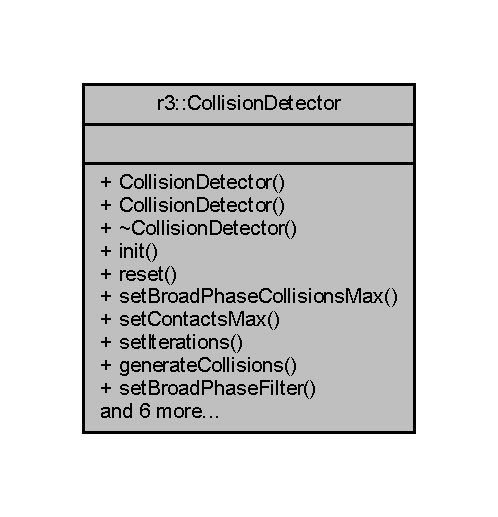
\includegraphics[width=239pt]{classr3_1_1_collision_detector__coll__graph}
\end{center}
\end{figure}
\subsection*{Public Types}
\begin{DoxyCompactItemize}
\item 
using \mbox{\hyperlink{classr3_1_1_collision_detector_aa8ed51d53c6f6ce545c93ad0e356d6de}{Broad\+Phase\+Filter\+\_\+\+Ptr}} = std\+::unique\+\_\+ptr$<$ \mbox{\hyperlink{classr3_1_1_i_broad_phase_filter}{I\+Broad\+Phase\+Filter}} $>$
\item 
using \mbox{\hyperlink{classr3_1_1_collision_detector_a8337c2c23ec77350b65977e043c07827}{Intermediate\+Phase\+Filter\+\_\+\+Ptr}} = std\+::unique\+\_\+ptr$<$ \mbox{\hyperlink{classr3_1_1_i_intermediate_phase_filter}{I\+Intermediate\+Phase\+Filter}} $>$
\item 
using \mbox{\hyperlink{classr3_1_1_collision_detector_a094cc287cba14d5a063cfca41e667008}{Narrow\+Phase\+Filter\+\_\+\+Ptr}} = std\+::unique\+\_\+ptr$<$ \mbox{\hyperlink{classr3_1_1_i_narrow_phase_filter}{I\+Narrow\+Phase\+Filter}} $>$
\end{DoxyCompactItemize}
\subsection*{Public Member Functions}
\begin{DoxyCompactItemize}
\item 
\mbox{\hyperlink{classr3_1_1_collision_detector_a8eaf42ee83c8bee06bc06601ec32c612}{Collision\+Detector}} (unsigned broad\+Phase\+Collisions=1000000, unsigned contacts\+Max=1000, unsigned iterations=2000)
\begin{DoxyCompactList}\small\item\em \mbox{\hyperlink{classr3_1_1_collision_detector}{Collision\+Detector}} constructor. \end{DoxyCompactList}\item 
\mbox{\hyperlink{classr3_1_1_collision_detector_ad44d67dd15e661d0e135016c89a7c9a4}{Collision\+Detector}} (const \mbox{\hyperlink{classr3_1_1_collision_detector}{Collision\+Detector}} \&)=delete
\item 
\mbox{\hyperlink{classr3_1_1_collision_detector_ab45ac57f6ab9bcab367e104e9423722a}{$\sim$\+Collision\+Detector}} ()
\item 
void \mbox{\hyperlink{classr3_1_1_collision_detector_a252e876b389dae66368afa210b93f31e}{init}} (unsigned broad\+Phase\+Collisions=1000000, unsigned contacts\+Max=1000, unsigned iterations=2000)
\begin{DoxyCompactList}\small\item\em Set the number of used contacts and iterations. \end{DoxyCompactList}\item 
void \mbox{\hyperlink{classr3_1_1_collision_detector_a8f9f9e0ecc67d950e79d024803dc916b}{reset}} ()
\begin{DoxyCompactList}\small\item\em Reset previously calculated collisions. \end{DoxyCompactList}\item 
void \mbox{\hyperlink{classr3_1_1_collision_detector_a386e4e4027a98c154423c8aea9079138}{set\+Broad\+Phase\+Collisions\+Max}} (int count)
\begin{DoxyCompactList}\small\item\em Set the maximal number of collision pairs created in the broad and intermediate phases. \end{DoxyCompactList}\item 
void \mbox{\hyperlink{classr3_1_1_collision_detector_a1920971e75d79df7806a8d803a010e62}{set\+Contacts\+Max}} (int count)
\begin{DoxyCompactList}\small\item\em Set the maximal number of contacts created in the narrow phase. \end{DoxyCompactList}\item 
void \mbox{\hyperlink{classr3_1_1_collision_detector_a4d6081592ca35150cd6c8fe0d551c64d}{set\+Iterations}} (int iterations)
\begin{DoxyCompactList}\small\item\em Set the maximal number of iterations used. \end{DoxyCompactList}\item 
\mbox{\hyperlink{classr3_1_1_collision_data}{Collision\+Data}} \& \mbox{\hyperlink{classr3_1_1_collision_detector_a58a1bd9705f241e4c137458bed35f596}{generate\+Collisions}} (const std\+::vector$<$ \mbox{\hyperlink{classr3_1_1_rigid_body}{Rigid\+Body}} $\ast$$>$ \&rigid\+Bodies)
\begin{DoxyCompactList}\small\item\em Generate a number of contacts for the given rigid bodies with the help of the current filters. \end{DoxyCompactList}\item 
void \mbox{\hyperlink{classr3_1_1_collision_detector_a2184ca2db73a6446cf028e3b742c7cc4}{set\+Broad\+Phase\+Filter}} (\mbox{\hyperlink{classr3_1_1_collision_detector_aa8ed51d53c6f6ce545c93ad0e356d6de}{Broad\+Phase\+Filter\+\_\+\+Ptr}} filter)
\begin{DoxyCompactList}\small\item\em Set the currently used broad phase filter. \end{DoxyCompactList}\item 
\mbox{\hyperlink{classr3_1_1_i_broad_phase_filter}{I\+Broad\+Phase\+Filter}} $\ast$ \mbox{\hyperlink{classr3_1_1_collision_detector_aa4d1c9560f806496b2215ddc623a1387}{get\+Broad\+Phase\+Filter}} () const
\begin{DoxyCompactList}\small\item\em Get the currently used broad phase filter. \end{DoxyCompactList}\item 
\mbox{\hyperlink{classr3_1_1_i_intermediate_phase_filter}{I\+Intermediate\+Phase\+Filter}} $\ast$ \mbox{\hyperlink{classr3_1_1_collision_detector_a804d66d43502a2b113aa1e8c302cebc7}{add\+Intermediate\+Phase\+Filter}} (\mbox{\hyperlink{classr3_1_1_collision_detector_a8337c2c23ec77350b65977e043c07827}{Intermediate\+Phase\+Filter\+\_\+\+Ptr}} filter)
\begin{DoxyCompactList}\small\item\em Add a new intermediate phase filter, which will be executed after all currently registered intermediate phase filters. \end{DoxyCompactList}\item 
\mbox{\hyperlink{classr3_1_1_collision_detector_a8337c2c23ec77350b65977e043c07827}{Intermediate\+Phase\+Filter\+\_\+\+Ptr}} \mbox{\hyperlink{classr3_1_1_collision_detector_aff67a43ffc0f74ada2193f46aa3ea1fd}{remove\+Intermediate\+Phase\+Filter}} (\mbox{\hyperlink{classr3_1_1_i_intermediate_phase_filter}{I\+Intermediate\+Phase\+Filter}} $\ast$filter)
\item 
void \mbox{\hyperlink{classr3_1_1_collision_detector_a780e977afd65d4a41863e712f9acb63f}{remove\+All\+Intermediate\+Phase\+Filters}} ()
\begin{DoxyCompactList}\small\item\em Clears the list of all currently registered intermediate phase filters. \end{DoxyCompactList}\item 
void \mbox{\hyperlink{classr3_1_1_collision_detector_a98f6ab749622d7fcffbdc0dcf59cfa75}{set\+Narrow\+Phase\+Filter}} (\mbox{\hyperlink{classr3_1_1_collision_detector_a094cc287cba14d5a063cfca41e667008}{Narrow\+Phase\+Filter\+\_\+\+Ptr}} filter)
\begin{DoxyCompactList}\small\item\em Set the currently used narrow phase filter. \end{DoxyCompactList}\item 
\mbox{\hyperlink{classr3_1_1_i_narrow_phase_filter}{I\+Narrow\+Phase\+Filter}} $\ast$ \mbox{\hyperlink{classr3_1_1_collision_detector_aa43b5d1332028d15a3c9af1ec4cd4312}{get\+Narrow\+Phase\+Filter}} () const
\begin{DoxyCompactList}\small\item\em Get the currently used narrow phase filter. \end{DoxyCompactList}\end{DoxyCompactItemize}


\subsection{Detailed Description}
The \mbox{\hyperlink{classr3_1_1_collision_detector}{Collision\+Detector}} acts as a batch controller (batch sequential). It executes collision detection filters (programs) in a specific order to generate contacts. 

\subsection{Member Typedef Documentation}
\mbox{\Hypertarget{classr3_1_1_collision_detector_aa8ed51d53c6f6ce545c93ad0e356d6de}\label{classr3_1_1_collision_detector_aa8ed51d53c6f6ce545c93ad0e356d6de}} 
\index{r3\+::\+Collision\+Detector@{r3\+::\+Collision\+Detector}!Broad\+Phase\+Filter\+\_\+\+Ptr@{Broad\+Phase\+Filter\+\_\+\+Ptr}}
\index{Broad\+Phase\+Filter\+\_\+\+Ptr@{Broad\+Phase\+Filter\+\_\+\+Ptr}!r3\+::\+Collision\+Detector@{r3\+::\+Collision\+Detector}}
\subsubsection{\texorpdfstring{Broad\+Phase\+Filter\+\_\+\+Ptr}{BroadPhaseFilter\_Ptr}}
{\footnotesize\ttfamily using \mbox{\hyperlink{classr3_1_1_collision_detector_aa8ed51d53c6f6ce545c93ad0e356d6de}{r3\+::\+Collision\+Detector\+::\+Broad\+Phase\+Filter\+\_\+\+Ptr}} =  std\+::unique\+\_\+ptr$<$\mbox{\hyperlink{classr3_1_1_i_broad_phase_filter}{I\+Broad\+Phase\+Filter}}$>$}

\mbox{\Hypertarget{classr3_1_1_collision_detector_a8337c2c23ec77350b65977e043c07827}\label{classr3_1_1_collision_detector_a8337c2c23ec77350b65977e043c07827}} 
\index{r3\+::\+Collision\+Detector@{r3\+::\+Collision\+Detector}!Intermediate\+Phase\+Filter\+\_\+\+Ptr@{Intermediate\+Phase\+Filter\+\_\+\+Ptr}}
\index{Intermediate\+Phase\+Filter\+\_\+\+Ptr@{Intermediate\+Phase\+Filter\+\_\+\+Ptr}!r3\+::\+Collision\+Detector@{r3\+::\+Collision\+Detector}}
\subsubsection{\texorpdfstring{Intermediate\+Phase\+Filter\+\_\+\+Ptr}{IntermediatePhaseFilter\_Ptr}}
{\footnotesize\ttfamily using \mbox{\hyperlink{classr3_1_1_collision_detector_a8337c2c23ec77350b65977e043c07827}{r3\+::\+Collision\+Detector\+::\+Intermediate\+Phase\+Filter\+\_\+\+Ptr}} =  std\+::unique\+\_\+ptr$<$\mbox{\hyperlink{classr3_1_1_i_intermediate_phase_filter}{I\+Intermediate\+Phase\+Filter}}$>$}

\mbox{\Hypertarget{classr3_1_1_collision_detector_a094cc287cba14d5a063cfca41e667008}\label{classr3_1_1_collision_detector_a094cc287cba14d5a063cfca41e667008}} 
\index{r3\+::\+Collision\+Detector@{r3\+::\+Collision\+Detector}!Narrow\+Phase\+Filter\+\_\+\+Ptr@{Narrow\+Phase\+Filter\+\_\+\+Ptr}}
\index{Narrow\+Phase\+Filter\+\_\+\+Ptr@{Narrow\+Phase\+Filter\+\_\+\+Ptr}!r3\+::\+Collision\+Detector@{r3\+::\+Collision\+Detector}}
\subsubsection{\texorpdfstring{Narrow\+Phase\+Filter\+\_\+\+Ptr}{NarrowPhaseFilter\_Ptr}}
{\footnotesize\ttfamily using \mbox{\hyperlink{classr3_1_1_collision_detector_a094cc287cba14d5a063cfca41e667008}{r3\+::\+Collision\+Detector\+::\+Narrow\+Phase\+Filter\+\_\+\+Ptr}} =  std\+::unique\+\_\+ptr$<$\mbox{\hyperlink{classr3_1_1_i_narrow_phase_filter}{I\+Narrow\+Phase\+Filter}}$>$}



\subsection{Constructor \& Destructor Documentation}
\mbox{\Hypertarget{classr3_1_1_collision_detector_a8eaf42ee83c8bee06bc06601ec32c612}\label{classr3_1_1_collision_detector_a8eaf42ee83c8bee06bc06601ec32c612}} 
\index{r3\+::\+Collision\+Detector@{r3\+::\+Collision\+Detector}!Collision\+Detector@{Collision\+Detector}}
\index{Collision\+Detector@{Collision\+Detector}!r3\+::\+Collision\+Detector@{r3\+::\+Collision\+Detector}}
\subsubsection{\texorpdfstring{Collision\+Detector()}{CollisionDetector()}\hspace{0.1cm}{\footnotesize\ttfamily [1/2]}}
{\footnotesize\ttfamily r3\+::\+Collision\+Detector\+::\+Collision\+Detector (\begin{DoxyParamCaption}\item[{unsigned}]{broad\+Phase\+Collisions = {\ttfamily 1000000},  }\item[{unsigned}]{contacts\+Max = {\ttfamily 1000},  }\item[{unsigned}]{iterations = {\ttfamily 2000} }\end{DoxyParamCaption})\hspace{0.3cm}{\ttfamily [explicit]}}



\mbox{\hyperlink{classr3_1_1_collision_detector}{Collision\+Detector}} constructor. 


\begin{DoxyParams}{Parameters}
{\em broad\+Phase\+Collisions} & The maximal number of collision that can be generated in the broad phase. \\
\hline
{\em contacts\+Max} & The maximal number of contacts that can be generated in the narrow phase. \\
\hline
{\em iterations} & The maximal number of iterations that can be used in contact generation. \\
\hline
\end{DoxyParams}
\mbox{\Hypertarget{classr3_1_1_collision_detector_ad44d67dd15e661d0e135016c89a7c9a4}\label{classr3_1_1_collision_detector_ad44d67dd15e661d0e135016c89a7c9a4}} 
\index{r3\+::\+Collision\+Detector@{r3\+::\+Collision\+Detector}!Collision\+Detector@{Collision\+Detector}}
\index{Collision\+Detector@{Collision\+Detector}!r3\+::\+Collision\+Detector@{r3\+::\+Collision\+Detector}}
\subsubsection{\texorpdfstring{Collision\+Detector()}{CollisionDetector()}\hspace{0.1cm}{\footnotesize\ttfamily [2/2]}}
{\footnotesize\ttfamily r3\+::\+Collision\+Detector\+::\+Collision\+Detector (\begin{DoxyParamCaption}\item[{const \mbox{\hyperlink{classr3_1_1_collision_detector}{Collision\+Detector}} \&}]{ }\end{DoxyParamCaption})\hspace{0.3cm}{\ttfamily [delete]}}

\mbox{\Hypertarget{classr3_1_1_collision_detector_ab45ac57f6ab9bcab367e104e9423722a}\label{classr3_1_1_collision_detector_ab45ac57f6ab9bcab367e104e9423722a}} 
\index{r3\+::\+Collision\+Detector@{r3\+::\+Collision\+Detector}!````~Collision\+Detector@{$\sim$\+Collision\+Detector}}
\index{````~Collision\+Detector@{$\sim$\+Collision\+Detector}!r3\+::\+Collision\+Detector@{r3\+::\+Collision\+Detector}}
\subsubsection{\texorpdfstring{$\sim$\+Collision\+Detector()}{~CollisionDetector()}}
{\footnotesize\ttfamily r3\+::\+Collision\+Detector\+::$\sim$\+Collision\+Detector (\begin{DoxyParamCaption}{ }\end{DoxyParamCaption})\hspace{0.3cm}{\ttfamily [default]}}



\subsection{Member Function Documentation}
\mbox{\Hypertarget{classr3_1_1_collision_detector_a804d66d43502a2b113aa1e8c302cebc7}\label{classr3_1_1_collision_detector_a804d66d43502a2b113aa1e8c302cebc7}} 
\index{r3\+::\+Collision\+Detector@{r3\+::\+Collision\+Detector}!add\+Intermediate\+Phase\+Filter@{add\+Intermediate\+Phase\+Filter}}
\index{add\+Intermediate\+Phase\+Filter@{add\+Intermediate\+Phase\+Filter}!r3\+::\+Collision\+Detector@{r3\+::\+Collision\+Detector}}
\subsubsection{\texorpdfstring{add\+Intermediate\+Phase\+Filter()}{addIntermediatePhaseFilter()}}
{\footnotesize\ttfamily \mbox{\hyperlink{classr3_1_1_i_intermediate_phase_filter}{I\+Intermediate\+Phase\+Filter}} $\ast$ r3\+::\+Collision\+Detector\+::add\+Intermediate\+Phase\+Filter (\begin{DoxyParamCaption}\item[{\mbox{\hyperlink{classr3_1_1_collision_detector_a8337c2c23ec77350b65977e043c07827}{Intermediate\+Phase\+Filter\+\_\+\+Ptr}}}]{filter }\end{DoxyParamCaption})}



Add a new intermediate phase filter, which will be executed after all currently registered intermediate phase filters. 


\begin{DoxyParams}{Parameters}
{\em filter} & The new intermediate phase filter \\
\hline
\end{DoxyParams}
\begin{DoxyReturn}{Returns}
The newly inserted intermediate phase filter. 
\end{DoxyReturn}
\mbox{\Hypertarget{classr3_1_1_collision_detector_a58a1bd9705f241e4c137458bed35f596}\label{classr3_1_1_collision_detector_a58a1bd9705f241e4c137458bed35f596}} 
\index{r3\+::\+Collision\+Detector@{r3\+::\+Collision\+Detector}!generate\+Collisions@{generate\+Collisions}}
\index{generate\+Collisions@{generate\+Collisions}!r3\+::\+Collision\+Detector@{r3\+::\+Collision\+Detector}}
\subsubsection{\texorpdfstring{generate\+Collisions()}{generateCollisions()}}
{\footnotesize\ttfamily \mbox{\hyperlink{classr3_1_1_collision_data}{Collision\+Data}} \& r3\+::\+Collision\+Detector\+::generate\+Collisions (\begin{DoxyParamCaption}\item[{const std\+::vector$<$ \mbox{\hyperlink{classr3_1_1_rigid_body}{Rigid\+Body}} $\ast$$>$ \&}]{rigid\+Bodies }\end{DoxyParamCaption})}



Generate a number of contacts for the given rigid bodies with the help of the current filters. 


\begin{DoxyParams}{Parameters}
{\em rigid\+Bodies} & The rigid bodies used for contact generation. \\
\hline
\end{DoxyParams}
\begin{DoxyReturn}{Returns}
The generated contacts. 
\end{DoxyReturn}
\mbox{\Hypertarget{classr3_1_1_collision_detector_aa4d1c9560f806496b2215ddc623a1387}\label{classr3_1_1_collision_detector_aa4d1c9560f806496b2215ddc623a1387}} 
\index{r3\+::\+Collision\+Detector@{r3\+::\+Collision\+Detector}!get\+Broad\+Phase\+Filter@{get\+Broad\+Phase\+Filter}}
\index{get\+Broad\+Phase\+Filter@{get\+Broad\+Phase\+Filter}!r3\+::\+Collision\+Detector@{r3\+::\+Collision\+Detector}}
\subsubsection{\texorpdfstring{get\+Broad\+Phase\+Filter()}{getBroadPhaseFilter()}}
{\footnotesize\ttfamily \mbox{\hyperlink{classr3_1_1_i_broad_phase_filter}{I\+Broad\+Phase\+Filter}} $\ast$ r3\+::\+Collision\+Detector\+::get\+Broad\+Phase\+Filter (\begin{DoxyParamCaption}{ }\end{DoxyParamCaption}) const}



Get the currently used broad phase filter. 

\begin{DoxyReturn}{Returns}
The broad phase filter. 
\end{DoxyReturn}
\mbox{\Hypertarget{classr3_1_1_collision_detector_aa43b5d1332028d15a3c9af1ec4cd4312}\label{classr3_1_1_collision_detector_aa43b5d1332028d15a3c9af1ec4cd4312}} 
\index{r3\+::\+Collision\+Detector@{r3\+::\+Collision\+Detector}!get\+Narrow\+Phase\+Filter@{get\+Narrow\+Phase\+Filter}}
\index{get\+Narrow\+Phase\+Filter@{get\+Narrow\+Phase\+Filter}!r3\+::\+Collision\+Detector@{r3\+::\+Collision\+Detector}}
\subsubsection{\texorpdfstring{get\+Narrow\+Phase\+Filter()}{getNarrowPhaseFilter()}}
{\footnotesize\ttfamily \mbox{\hyperlink{classr3_1_1_i_narrow_phase_filter}{I\+Narrow\+Phase\+Filter}} $\ast$ r3\+::\+Collision\+Detector\+::get\+Narrow\+Phase\+Filter (\begin{DoxyParamCaption}{ }\end{DoxyParamCaption}) const}



Get the currently used narrow phase filter. 

\begin{DoxyReturn}{Returns}
The narrow phase filter. 
\end{DoxyReturn}
\mbox{\Hypertarget{classr3_1_1_collision_detector_a252e876b389dae66368afa210b93f31e}\label{classr3_1_1_collision_detector_a252e876b389dae66368afa210b93f31e}} 
\index{r3\+::\+Collision\+Detector@{r3\+::\+Collision\+Detector}!init@{init}}
\index{init@{init}!r3\+::\+Collision\+Detector@{r3\+::\+Collision\+Detector}}
\subsubsection{\texorpdfstring{init()}{init()}}
{\footnotesize\ttfamily void r3\+::\+Collision\+Detector\+::init (\begin{DoxyParamCaption}\item[{unsigned}]{broad\+Phase\+Collisions = {\ttfamily 1000000},  }\item[{unsigned}]{contacts\+Max = {\ttfamily 1000},  }\item[{unsigned}]{iterations = {\ttfamily 2000} }\end{DoxyParamCaption})}



Set the number of used contacts and iterations. 


\begin{DoxyParams}{Parameters}
{\em broad\+Phase\+Collisions} & The maximal number of collision that can be generated in the broad phase. \\
\hline
{\em contacts\+Max} & The maximal number of contacts that can be generated in the narrow phase. \\
\hline
{\em iterations} & The maximal number of iterations that can be used in contact generation. \\
\hline
\end{DoxyParams}
\mbox{\Hypertarget{classr3_1_1_collision_detector_a780e977afd65d4a41863e712f9acb63f}\label{classr3_1_1_collision_detector_a780e977afd65d4a41863e712f9acb63f}} 
\index{r3\+::\+Collision\+Detector@{r3\+::\+Collision\+Detector}!remove\+All\+Intermediate\+Phase\+Filters@{remove\+All\+Intermediate\+Phase\+Filters}}
\index{remove\+All\+Intermediate\+Phase\+Filters@{remove\+All\+Intermediate\+Phase\+Filters}!r3\+::\+Collision\+Detector@{r3\+::\+Collision\+Detector}}
\subsubsection{\texorpdfstring{remove\+All\+Intermediate\+Phase\+Filters()}{removeAllIntermediatePhaseFilters()}}
{\footnotesize\ttfamily void r3\+::\+Collision\+Detector\+::remove\+All\+Intermediate\+Phase\+Filters (\begin{DoxyParamCaption}{ }\end{DoxyParamCaption})}



Clears the list of all currently registered intermediate phase filters. 

\mbox{\Hypertarget{classr3_1_1_collision_detector_aff67a43ffc0f74ada2193f46aa3ea1fd}\label{classr3_1_1_collision_detector_aff67a43ffc0f74ada2193f46aa3ea1fd}} 
\index{r3\+::\+Collision\+Detector@{r3\+::\+Collision\+Detector}!remove\+Intermediate\+Phase\+Filter@{remove\+Intermediate\+Phase\+Filter}}
\index{remove\+Intermediate\+Phase\+Filter@{remove\+Intermediate\+Phase\+Filter}!r3\+::\+Collision\+Detector@{r3\+::\+Collision\+Detector}}
\subsubsection{\texorpdfstring{remove\+Intermediate\+Phase\+Filter()}{removeIntermediatePhaseFilter()}}
{\footnotesize\ttfamily \mbox{\hyperlink{classr3_1_1_collision_detector_a8337c2c23ec77350b65977e043c07827}{Collision\+Detector\+::\+Intermediate\+Phase\+Filter\+\_\+\+Ptr}} r3\+::\+Collision\+Detector\+::remove\+Intermediate\+Phase\+Filter (\begin{DoxyParamCaption}\item[{\mbox{\hyperlink{classr3_1_1_i_intermediate_phase_filter}{I\+Intermediate\+Phase\+Filter}} $\ast$}]{filter }\end{DoxyParamCaption})}

Remove the given filter from the current list of registered intermediate phase filters. \begin{DoxyReturn}{Returns}
True if the given filter was found and removed, false otherwise. 
\end{DoxyReturn}
\mbox{\Hypertarget{classr3_1_1_collision_detector_a8f9f9e0ecc67d950e79d024803dc916b}\label{classr3_1_1_collision_detector_a8f9f9e0ecc67d950e79d024803dc916b}} 
\index{r3\+::\+Collision\+Detector@{r3\+::\+Collision\+Detector}!reset@{reset}}
\index{reset@{reset}!r3\+::\+Collision\+Detector@{r3\+::\+Collision\+Detector}}
\subsubsection{\texorpdfstring{reset()}{reset()}}
{\footnotesize\ttfamily void r3\+::\+Collision\+Detector\+::reset (\begin{DoxyParamCaption}{ }\end{DoxyParamCaption})}



Reset previously calculated collisions. 

\mbox{\Hypertarget{classr3_1_1_collision_detector_a386e4e4027a98c154423c8aea9079138}\label{classr3_1_1_collision_detector_a386e4e4027a98c154423c8aea9079138}} 
\index{r3\+::\+Collision\+Detector@{r3\+::\+Collision\+Detector}!set\+Broad\+Phase\+Collisions\+Max@{set\+Broad\+Phase\+Collisions\+Max}}
\index{set\+Broad\+Phase\+Collisions\+Max@{set\+Broad\+Phase\+Collisions\+Max}!r3\+::\+Collision\+Detector@{r3\+::\+Collision\+Detector}}
\subsubsection{\texorpdfstring{set\+Broad\+Phase\+Collisions\+Max()}{setBroadPhaseCollisionsMax()}}
{\footnotesize\ttfamily void r3\+::\+Collision\+Detector\+::set\+Broad\+Phase\+Collisions\+Max (\begin{DoxyParamCaption}\item[{int}]{count }\end{DoxyParamCaption})}



Set the maximal number of collision pairs created in the broad and intermediate phases. 


\begin{DoxyParams}{Parameters}
{\em count} & The maximal number of collision pairs that can be generated in the broad phase. \\
\hline
\end{DoxyParams}
\mbox{\Hypertarget{classr3_1_1_collision_detector_a2184ca2db73a6446cf028e3b742c7cc4}\label{classr3_1_1_collision_detector_a2184ca2db73a6446cf028e3b742c7cc4}} 
\index{r3\+::\+Collision\+Detector@{r3\+::\+Collision\+Detector}!set\+Broad\+Phase\+Filter@{set\+Broad\+Phase\+Filter}}
\index{set\+Broad\+Phase\+Filter@{set\+Broad\+Phase\+Filter}!r3\+::\+Collision\+Detector@{r3\+::\+Collision\+Detector}}
\subsubsection{\texorpdfstring{set\+Broad\+Phase\+Filter()}{setBroadPhaseFilter()}}
{\footnotesize\ttfamily void r3\+::\+Collision\+Detector\+::set\+Broad\+Phase\+Filter (\begin{DoxyParamCaption}\item[{\mbox{\hyperlink{classr3_1_1_collision_detector_aa8ed51d53c6f6ce545c93ad0e356d6de}{Broad\+Phase\+Filter\+\_\+\+Ptr}}}]{filter }\end{DoxyParamCaption})}



Set the currently used broad phase filter. 


\begin{DoxyParams}{Parameters}
{\em filter} & The broad phase filter. \\
\hline
\end{DoxyParams}
\mbox{\Hypertarget{classr3_1_1_collision_detector_a1920971e75d79df7806a8d803a010e62}\label{classr3_1_1_collision_detector_a1920971e75d79df7806a8d803a010e62}} 
\index{r3\+::\+Collision\+Detector@{r3\+::\+Collision\+Detector}!set\+Contacts\+Max@{set\+Contacts\+Max}}
\index{set\+Contacts\+Max@{set\+Contacts\+Max}!r3\+::\+Collision\+Detector@{r3\+::\+Collision\+Detector}}
\subsubsection{\texorpdfstring{set\+Contacts\+Max()}{setContactsMax()}}
{\footnotesize\ttfamily void r3\+::\+Collision\+Detector\+::set\+Contacts\+Max (\begin{DoxyParamCaption}\item[{int}]{count }\end{DoxyParamCaption})}



Set the maximal number of contacts created in the narrow phase. 


\begin{DoxyParams}{Parameters}
{\em count} & The maximal number of contacts. \\
\hline
\end{DoxyParams}
\mbox{\Hypertarget{classr3_1_1_collision_detector_a4d6081592ca35150cd6c8fe0d551c64d}\label{classr3_1_1_collision_detector_a4d6081592ca35150cd6c8fe0d551c64d}} 
\index{r3\+::\+Collision\+Detector@{r3\+::\+Collision\+Detector}!set\+Iterations@{set\+Iterations}}
\index{set\+Iterations@{set\+Iterations}!r3\+::\+Collision\+Detector@{r3\+::\+Collision\+Detector}}
\subsubsection{\texorpdfstring{set\+Iterations()}{setIterations()}}
{\footnotesize\ttfamily void r3\+::\+Collision\+Detector\+::set\+Iterations (\begin{DoxyParamCaption}\item[{int}]{iterations }\end{DoxyParamCaption})}



Set the maximal number of iterations used. 


\begin{DoxyParams}{Parameters}
{\em iterations} & The maximal number of iterations. \\
\hline
\end{DoxyParams}
\mbox{\Hypertarget{classr3_1_1_collision_detector_a98f6ab749622d7fcffbdc0dcf59cfa75}\label{classr3_1_1_collision_detector_a98f6ab749622d7fcffbdc0dcf59cfa75}} 
\index{r3\+::\+Collision\+Detector@{r3\+::\+Collision\+Detector}!set\+Narrow\+Phase\+Filter@{set\+Narrow\+Phase\+Filter}}
\index{set\+Narrow\+Phase\+Filter@{set\+Narrow\+Phase\+Filter}!r3\+::\+Collision\+Detector@{r3\+::\+Collision\+Detector}}
\subsubsection{\texorpdfstring{set\+Narrow\+Phase\+Filter()}{setNarrowPhaseFilter()}}
{\footnotesize\ttfamily void r3\+::\+Collision\+Detector\+::set\+Narrow\+Phase\+Filter (\begin{DoxyParamCaption}\item[{\mbox{\hyperlink{classr3_1_1_collision_detector_a094cc287cba14d5a063cfca41e667008}{Narrow\+Phase\+Filter\+\_\+\+Ptr}}}]{filter }\end{DoxyParamCaption})}



Set the currently used narrow phase filter. 


\begin{DoxyParams}{Parameters}
{\em filter} & The new narrow phase filter. \\
\hline
\end{DoxyParams}


The documentation for this class was generated from the following files\+:\begin{DoxyCompactItemize}
\item 
C\+:/\+Library/\+Job/\+Projekte/\+Simulation\+Visualization/\+Rumble3\+D/\+Rumble3\+D/include/\+R3\+D/\+Rigid\+Body\+Engine/\+Collision\+Detection/\mbox{\hyperlink{_collision_detector_8h}{Collision\+Detector.\+h}}\item 
C\+:/\+Library/\+Job/\+Projekte/\+Simulation\+Visualization/\+Rumble3\+D/\+Rumble3\+D/src/\+Rigid\+Body\+Engine/\+Collision\+Detection/\mbox{\hyperlink{_collision_detector_8cpp}{Collision\+Detector.\+cpp}}\end{DoxyCompactItemize}

\hypertarget{classr3_1_1_collision_detector_old}{}\section{r3\+:\+:Collision\+Detector\+Old Class Reference}
\label{classr3_1_1_collision_detector_old}\index{r3\+::\+Collision\+Detector\+Old@{r3\+::\+Collision\+Detector\+Old}}


{\ttfamily \#include $<$Collision\+Detector\+Old.\+h$>$}



Collaboration diagram for r3\+:\+:Collision\+Detector\+Old\+:\nopagebreak
\begin{figure}[H]
\begin{center}
\leavevmode
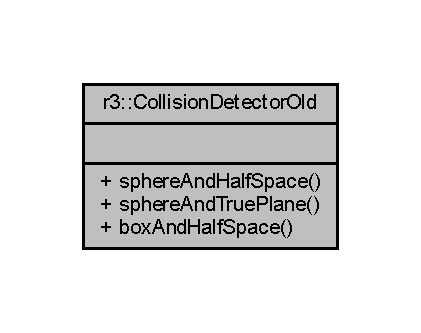
\includegraphics[width=202pt]{classr3_1_1_collision_detector_old__coll__graph}
\end{center}
\end{figure}
\subsection*{Static Public Member Functions}
\begin{DoxyCompactItemize}
\item 
static unsigned \mbox{\hyperlink{classr3_1_1_collision_detector_old_afac2bf8c0034f33fee66979d69da76e7}{sphere\+And\+Half\+Space}} (const \mbox{\hyperlink{classr3_1_1_collision_sphere}{Collision\+Sphere}} \&sphere, const \mbox{\hyperlink{classr3_1_1_collision_plane}{Collision\+Plane}} \&plane, \mbox{\hyperlink{classr3_1_1_collision_data_old}{Collision\+Data\+Old}} $\ast$data)
\item 
static unsigned \mbox{\hyperlink{classr3_1_1_collision_detector_old_ac193fb110bfd2618ed61aa59b72c6877}{sphere\+And\+True\+Plane}} (const \mbox{\hyperlink{classr3_1_1_collision_sphere}{Collision\+Sphere}} \&sphere, const \mbox{\hyperlink{classr3_1_1_collision_plane}{Collision\+Plane}} \&plane, \mbox{\hyperlink{classr3_1_1_collision_data_old}{Collision\+Data\+Old}} $\ast$data)
\item 
static unsigned \mbox{\hyperlink{classr3_1_1_collision_detector_old_a947191d7a2503e4475d3a9098009601e}{sphere\+And\+Sphere}} (const \mbox{\hyperlink{classr3_1_1_collision_sphere}{Collision\+Sphere}} \&one, const \mbox{\hyperlink{classr3_1_1_collision_sphere}{Collision\+Sphere}} \&two, \mbox{\hyperlink{classr3_1_1_collision_data_old}{Collision\+Data\+Old}} $\ast$data)
\item 
static unsigned \mbox{\hyperlink{classr3_1_1_collision_detector_old_ad1fa9c247235130c96432fc3f5524e8f}{box\+And\+Half\+Space}} (const \mbox{\hyperlink{classr3_1_1_collision_box}{Collision\+Box}} \&box, const \mbox{\hyperlink{classr3_1_1_collision_plane}{Collision\+Plane}} \&plane, \mbox{\hyperlink{classr3_1_1_collision_data_old}{Collision\+Data\+Old}} $\ast$data)
\item 
static unsigned \mbox{\hyperlink{classr3_1_1_collision_detector_old_a16fabd7a2ded98f3cb7694f853724541}{box\+And\+Sphere}} (const \mbox{\hyperlink{classr3_1_1_collision_box}{Collision\+Box}} \&box, const \mbox{\hyperlink{classr3_1_1_collision_sphere}{Collision\+Sphere}} \&sphere, \mbox{\hyperlink{classr3_1_1_collision_data_old}{Collision\+Data\+Old}} $\ast$data)
\item 
static unsigned \mbox{\hyperlink{classr3_1_1_collision_detector_old_afd98d9fbaa8ace5bb239a2a2da08aace}{box\+And\+Box}} (const \mbox{\hyperlink{classr3_1_1_collision_box}{Collision\+Box}} \&one, const \mbox{\hyperlink{classr3_1_1_collision_box}{Collision\+Box}} \&two, \mbox{\hyperlink{classr3_1_1_collision_data_old}{Collision\+Data\+Old}} $\ast$data)
\end{DoxyCompactItemize}


\subsection{Member Function Documentation}
\mbox{\Hypertarget{classr3_1_1_collision_detector_old_afd98d9fbaa8ace5bb239a2a2da08aace}\label{classr3_1_1_collision_detector_old_afd98d9fbaa8ace5bb239a2a2da08aace}} 
\index{r3\+::\+Collision\+Detector\+Old@{r3\+::\+Collision\+Detector\+Old}!box\+And\+Box@{box\+And\+Box}}
\index{box\+And\+Box@{box\+And\+Box}!r3\+::\+Collision\+Detector\+Old@{r3\+::\+Collision\+Detector\+Old}}
\subsubsection{\texorpdfstring{box\+And\+Box()}{boxAndBox()}}
{\footnotesize\ttfamily unsigned r3\+::\+Collision\+Detector\+Old\+::box\+And\+Box (\begin{DoxyParamCaption}\item[{const \mbox{\hyperlink{classr3_1_1_collision_box}{Collision\+Box}} \&}]{one,  }\item[{const \mbox{\hyperlink{classr3_1_1_collision_box}{Collision\+Box}} \&}]{two,  }\item[{\mbox{\hyperlink{classr3_1_1_collision_data_old}{Collision\+Data\+Old}} $\ast$}]{data }\end{DoxyParamCaption})\hspace{0.3cm}{\ttfamily [static]}}

\begin{DoxyRefDesc}{Todo}
\item[\mbox{\hyperlink{todo__todo000006}{Todo}}]variable is never set??? \end{DoxyRefDesc}
\mbox{\Hypertarget{classr3_1_1_collision_detector_old_ad1fa9c247235130c96432fc3f5524e8f}\label{classr3_1_1_collision_detector_old_ad1fa9c247235130c96432fc3f5524e8f}} 
\index{r3\+::\+Collision\+Detector\+Old@{r3\+::\+Collision\+Detector\+Old}!box\+And\+Half\+Space@{box\+And\+Half\+Space}}
\index{box\+And\+Half\+Space@{box\+And\+Half\+Space}!r3\+::\+Collision\+Detector\+Old@{r3\+::\+Collision\+Detector\+Old}}
\subsubsection{\texorpdfstring{box\+And\+Half\+Space()}{boxAndHalfSpace()}}
{\footnotesize\ttfamily unsigned r3\+::\+Collision\+Detector\+Old\+::box\+And\+Half\+Space (\begin{DoxyParamCaption}\item[{const \mbox{\hyperlink{classr3_1_1_collision_box}{Collision\+Box}} \&}]{box,  }\item[{const \mbox{\hyperlink{classr3_1_1_collision_plane}{Collision\+Plane}} \&}]{plane,  }\item[{\mbox{\hyperlink{classr3_1_1_collision_data_old}{Collision\+Data\+Old}} $\ast$}]{data }\end{DoxyParamCaption})\hspace{0.3cm}{\ttfamily [static]}}

\mbox{\Hypertarget{classr3_1_1_collision_detector_old_a16fabd7a2ded98f3cb7694f853724541}\label{classr3_1_1_collision_detector_old_a16fabd7a2ded98f3cb7694f853724541}} 
\index{r3\+::\+Collision\+Detector\+Old@{r3\+::\+Collision\+Detector\+Old}!box\+And\+Sphere@{box\+And\+Sphere}}
\index{box\+And\+Sphere@{box\+And\+Sphere}!r3\+::\+Collision\+Detector\+Old@{r3\+::\+Collision\+Detector\+Old}}
\subsubsection{\texorpdfstring{box\+And\+Sphere()}{boxAndSphere()}}
{\footnotesize\ttfamily unsigned r3\+::\+Collision\+Detector\+Old\+::box\+And\+Sphere (\begin{DoxyParamCaption}\item[{const \mbox{\hyperlink{classr3_1_1_collision_box}{Collision\+Box}} \&}]{box,  }\item[{const \mbox{\hyperlink{classr3_1_1_collision_sphere}{Collision\+Sphere}} \&}]{sphere,  }\item[{\mbox{\hyperlink{classr3_1_1_collision_data_old}{Collision\+Data\+Old}} $\ast$}]{data }\end{DoxyParamCaption})\hspace{0.3cm}{\ttfamily [static]}}

\mbox{\Hypertarget{classr3_1_1_collision_detector_old_afac2bf8c0034f33fee66979d69da76e7}\label{classr3_1_1_collision_detector_old_afac2bf8c0034f33fee66979d69da76e7}} 
\index{r3\+::\+Collision\+Detector\+Old@{r3\+::\+Collision\+Detector\+Old}!sphere\+And\+Half\+Space@{sphere\+And\+Half\+Space}}
\index{sphere\+And\+Half\+Space@{sphere\+And\+Half\+Space}!r3\+::\+Collision\+Detector\+Old@{r3\+::\+Collision\+Detector\+Old}}
\subsubsection{\texorpdfstring{sphere\+And\+Half\+Space()}{sphereAndHalfSpace()}}
{\footnotesize\ttfamily unsigned r3\+::\+Collision\+Detector\+Old\+::sphere\+And\+Half\+Space (\begin{DoxyParamCaption}\item[{const \mbox{\hyperlink{classr3_1_1_collision_sphere}{Collision\+Sphere}} \&}]{sphere,  }\item[{const \mbox{\hyperlink{classr3_1_1_collision_plane}{Collision\+Plane}} \&}]{plane,  }\item[{\mbox{\hyperlink{classr3_1_1_collision_data_old}{Collision\+Data\+Old}} $\ast$}]{data }\end{DoxyParamCaption})\hspace{0.3cm}{\ttfamily [static]}}

\mbox{\Hypertarget{classr3_1_1_collision_detector_old_a947191d7a2503e4475d3a9098009601e}\label{classr3_1_1_collision_detector_old_a947191d7a2503e4475d3a9098009601e}} 
\index{r3\+::\+Collision\+Detector\+Old@{r3\+::\+Collision\+Detector\+Old}!sphere\+And\+Sphere@{sphere\+And\+Sphere}}
\index{sphere\+And\+Sphere@{sphere\+And\+Sphere}!r3\+::\+Collision\+Detector\+Old@{r3\+::\+Collision\+Detector\+Old}}
\subsubsection{\texorpdfstring{sphere\+And\+Sphere()}{sphereAndSphere()}}
{\footnotesize\ttfamily unsigned r3\+::\+Collision\+Detector\+Old\+::sphere\+And\+Sphere (\begin{DoxyParamCaption}\item[{const \mbox{\hyperlink{classr3_1_1_collision_sphere}{Collision\+Sphere}} \&}]{one,  }\item[{const \mbox{\hyperlink{classr3_1_1_collision_sphere}{Collision\+Sphere}} \&}]{two,  }\item[{\mbox{\hyperlink{classr3_1_1_collision_data_old}{Collision\+Data\+Old}} $\ast$}]{data }\end{DoxyParamCaption})\hspace{0.3cm}{\ttfamily [static]}}

\mbox{\Hypertarget{classr3_1_1_collision_detector_old_ac193fb110bfd2618ed61aa59b72c6877}\label{classr3_1_1_collision_detector_old_ac193fb110bfd2618ed61aa59b72c6877}} 
\index{r3\+::\+Collision\+Detector\+Old@{r3\+::\+Collision\+Detector\+Old}!sphere\+And\+True\+Plane@{sphere\+And\+True\+Plane}}
\index{sphere\+And\+True\+Plane@{sphere\+And\+True\+Plane}!r3\+::\+Collision\+Detector\+Old@{r3\+::\+Collision\+Detector\+Old}}
\subsubsection{\texorpdfstring{sphere\+And\+True\+Plane()}{sphereAndTruePlane()}}
{\footnotesize\ttfamily unsigned r3\+::\+Collision\+Detector\+Old\+::sphere\+And\+True\+Plane (\begin{DoxyParamCaption}\item[{const \mbox{\hyperlink{classr3_1_1_collision_sphere}{Collision\+Sphere}} \&}]{sphere,  }\item[{const \mbox{\hyperlink{classr3_1_1_collision_plane}{Collision\+Plane}} \&}]{plane,  }\item[{\mbox{\hyperlink{classr3_1_1_collision_data_old}{Collision\+Data\+Old}} $\ast$}]{data }\end{DoxyParamCaption})\hspace{0.3cm}{\ttfamily [static]}}



The documentation for this class was generated from the following files\+:\begin{DoxyCompactItemize}
\item 
D\+:/\+Library/\+Documents/\+Job/\+Forschungsmaster/\+Projekte/\+Simulation\+Visualization/\+Rumble3\+D/\+Rumble3\+D/include/\+R3\+D/\+Rigid\+Body\+Engine/\mbox{\hyperlink{_collision_detector_old_8h}{Collision\+Detector\+Old.\+h}}\item 
D\+:/\+Library/\+Documents/\+Job/\+Forschungsmaster/\+Projekte/\+Simulation\+Visualization/\+Rumble3\+D/\+Rumble3\+D/src/\+Rigid\+Body\+Engine/\mbox{\hyperlink{_collision_detector_old_8cpp}{Collision\+Detector\+Old.\+cpp}}\end{DoxyCompactItemize}

\hypertarget{structr3_1_1_collision_mask}{}\section{r3\+:\+:Collision\+Mask Struct Reference}
\label{structr3_1_1_collision_mask}\index{r3\+::\+Collision\+Mask@{r3\+::\+Collision\+Mask}}


Used to group rigid bodies. Only rigid bodies from the same layer can collide. Rigid bodies from the same group cannot collide!  




{\ttfamily \#include $<$Collision\+Mask.\+h$>$}



Collaboration diagram for r3\+:\+:Collision\+Mask\+:\nopagebreak
\begin{figure}[H]
\begin{center}
\leavevmode
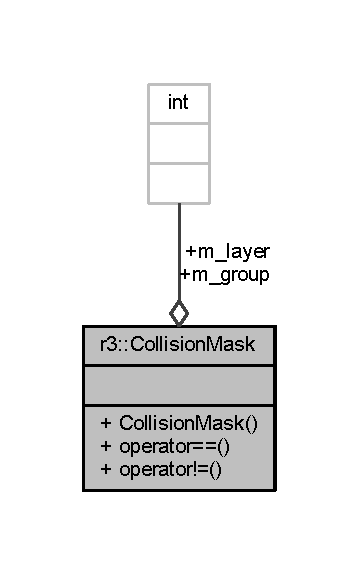
\includegraphics[width=172pt]{structr3_1_1_collision_mask__coll__graph}
\end{center}
\end{figure}
\subsection*{Public Member Functions}
\begin{DoxyCompactItemize}
\item 
\mbox{\hyperlink{structr3_1_1_collision_mask_a7f1fb1fae3d7e14677ad2590fcd661e0}{Collision\+Mask}} (unsigned int layer=0, unsigned int group=0)
\begin{DoxyCompactList}\small\item\em \mbox{\hyperlink{structr3_1_1_collision_mask}{Collision\+Mask}} constructor. \end{DoxyCompactList}\item 
bool \mbox{\hyperlink{structr3_1_1_collision_mask_a7d1315f7324fc03cee09df2c364f5c54}{operator==}} (const \mbox{\hyperlink{structr3_1_1_collision_mask}{Collision\+Mask}} \&mask) const
\item 
bool \mbox{\hyperlink{structr3_1_1_collision_mask_ae6bbe0e4390b584497c854d39ec12c6a}{operator!=}} (const \mbox{\hyperlink{structr3_1_1_collision_mask}{Collision\+Mask}} \&mask) const
\end{DoxyCompactItemize}
\subsection*{Public Attributes}
\begin{DoxyCompactItemize}
\item 
unsigned int \mbox{\hyperlink{structr3_1_1_collision_mask_a07999f53c748c86623b00e4e07d24d5f}{m\+\_\+group}}
\item 
unsigned int \mbox{\hyperlink{structr3_1_1_collision_mask_a4e3ed2227bb1782f7c6dc948a8427620}{m\+\_\+layer}}
\end{DoxyCompactItemize}


\subsection{Detailed Description}
Used to group rigid bodies. Only rigid bodies from the same layer can collide. Rigid bodies from the same group cannot collide! 

\subsection{Constructor \& Destructor Documentation}
\mbox{\Hypertarget{structr3_1_1_collision_mask_a7f1fb1fae3d7e14677ad2590fcd661e0}\label{structr3_1_1_collision_mask_a7f1fb1fae3d7e14677ad2590fcd661e0}} 
\index{r3\+::\+Collision\+Mask@{r3\+::\+Collision\+Mask}!Collision\+Mask@{Collision\+Mask}}
\index{Collision\+Mask@{Collision\+Mask}!r3\+::\+Collision\+Mask@{r3\+::\+Collision\+Mask}}
\subsubsection{\texorpdfstring{Collision\+Mask()}{CollisionMask()}}
{\footnotesize\ttfamily r3\+::\+Collision\+Mask\+::\+Collision\+Mask (\begin{DoxyParamCaption}\item[{unsigned int}]{layer = {\ttfamily 0},  }\item[{unsigned int}]{group = {\ttfamily 0} }\end{DoxyParamCaption})\hspace{0.3cm}{\ttfamily [explicit]}}



\mbox{\hyperlink{structr3_1_1_collision_mask}{Collision\+Mask}} constructor. 


\begin{DoxyParams}{Parameters}
{\em layer} & Only bodies from the same layer can collide. \\
\hline
{\em group} & Bodies from the same group can\textquotesingle{}t collide. \\
\hline
\end{DoxyParams}


\subsection{Member Function Documentation}
\mbox{\Hypertarget{structr3_1_1_collision_mask_ae6bbe0e4390b584497c854d39ec12c6a}\label{structr3_1_1_collision_mask_ae6bbe0e4390b584497c854d39ec12c6a}} 
\index{r3\+::\+Collision\+Mask@{r3\+::\+Collision\+Mask}!operator"!=@{operator"!=}}
\index{operator"!=@{operator"!=}!r3\+::\+Collision\+Mask@{r3\+::\+Collision\+Mask}}
\subsubsection{\texorpdfstring{operator"!=()}{operator!=()}}
{\footnotesize\ttfamily bool r3\+::\+Collision\+Mask\+::operator!= (\begin{DoxyParamCaption}\item[{const \mbox{\hyperlink{structr3_1_1_collision_mask}{Collision\+Mask}} \&}]{mask }\end{DoxyParamCaption}) const}

\mbox{\Hypertarget{structr3_1_1_collision_mask_a7d1315f7324fc03cee09df2c364f5c54}\label{structr3_1_1_collision_mask_a7d1315f7324fc03cee09df2c364f5c54}} 
\index{r3\+::\+Collision\+Mask@{r3\+::\+Collision\+Mask}!operator==@{operator==}}
\index{operator==@{operator==}!r3\+::\+Collision\+Mask@{r3\+::\+Collision\+Mask}}
\subsubsection{\texorpdfstring{operator==()}{operator==()}}
{\footnotesize\ttfamily bool r3\+::\+Collision\+Mask\+::operator== (\begin{DoxyParamCaption}\item[{const \mbox{\hyperlink{structr3_1_1_collision_mask}{Collision\+Mask}} \&}]{mask }\end{DoxyParamCaption}) const}



\subsection{Member Data Documentation}
\mbox{\Hypertarget{structr3_1_1_collision_mask_a07999f53c748c86623b00e4e07d24d5f}\label{structr3_1_1_collision_mask_a07999f53c748c86623b00e4e07d24d5f}} 
\index{r3\+::\+Collision\+Mask@{r3\+::\+Collision\+Mask}!m\+\_\+group@{m\+\_\+group}}
\index{m\+\_\+group@{m\+\_\+group}!r3\+::\+Collision\+Mask@{r3\+::\+Collision\+Mask}}
\subsubsection{\texorpdfstring{m\+\_\+group}{m\_group}}
{\footnotesize\ttfamily unsigned int r3\+::\+Collision\+Mask\+::m\+\_\+group}

\mbox{\Hypertarget{structr3_1_1_collision_mask_a4e3ed2227bb1782f7c6dc948a8427620}\label{structr3_1_1_collision_mask_a4e3ed2227bb1782f7c6dc948a8427620}} 
\index{r3\+::\+Collision\+Mask@{r3\+::\+Collision\+Mask}!m\+\_\+layer@{m\+\_\+layer}}
\index{m\+\_\+layer@{m\+\_\+layer}!r3\+::\+Collision\+Mask@{r3\+::\+Collision\+Mask}}
\subsubsection{\texorpdfstring{m\+\_\+layer}{m\_layer}}
{\footnotesize\ttfamily unsigned int r3\+::\+Collision\+Mask\+::m\+\_\+layer}



The documentation for this struct was generated from the following files\+:\begin{DoxyCompactItemize}
\item 
D\+:/\+Library/\+Documents/\+Job/\+Forschungsmaster/\+Projekte/\+Simulation\+Visualization/\+Rumble3\+D/\+Rumble3\+D/include/\+R3\+D/\+Rigid\+Body\+Engine/\+Collision\+Detection/\mbox{\hyperlink{_collision_mask_8h}{Collision\+Mask.\+h}}\item 
D\+:/\+Library/\+Documents/\+Job/\+Forschungsmaster/\+Projekte/\+Simulation\+Visualization/\+Rumble3\+D/\+Rumble3\+D/src/\+Rigid\+Body\+Engine/\+Collision\+Detection/\mbox{\hyperlink{_collision_mask_8cpp}{Collision\+Mask.\+cpp}}\end{DoxyCompactItemize}

\hypertarget{classr3_1_1_collision_object}{}\section{r3\+:\+:Collision\+Object Class Reference}
\label{classr3_1_1_collision_object}\index{r3\+::\+Collision\+Object@{r3\+::\+Collision\+Object}}


{\ttfamily \#include $<$Collision\+Object.\+h$>$}



Inheritance diagram for r3\+:\+:Collision\+Object\+:\nopagebreak
\begin{figure}[H]
\begin{center}
\leavevmode
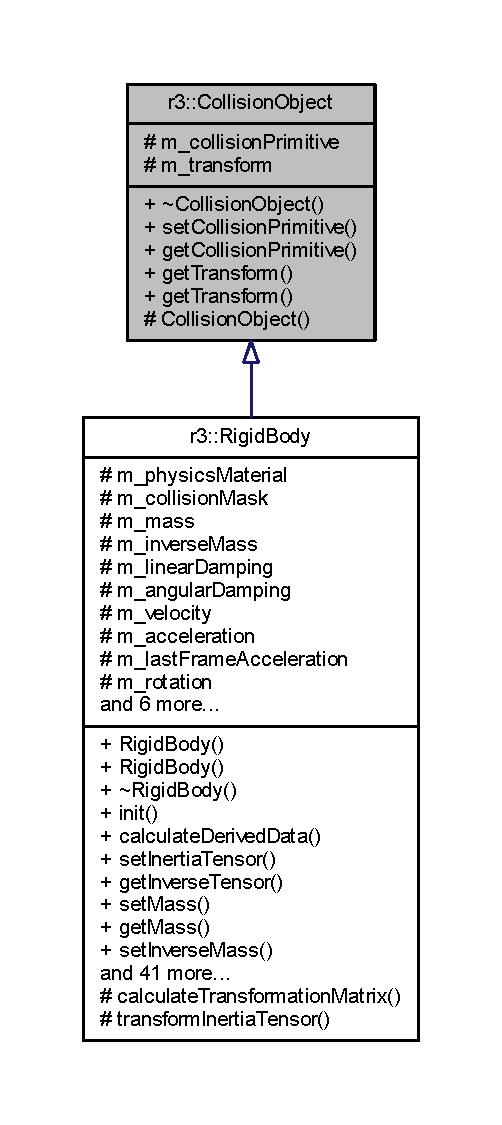
\includegraphics[width=241pt]{classr3_1_1_collision_object__inherit__graph}
\end{center}
\end{figure}


Collaboration diagram for r3\+:\+:Collision\+Object\+:\nopagebreak
\begin{figure}[H]
\begin{center}
\leavevmode
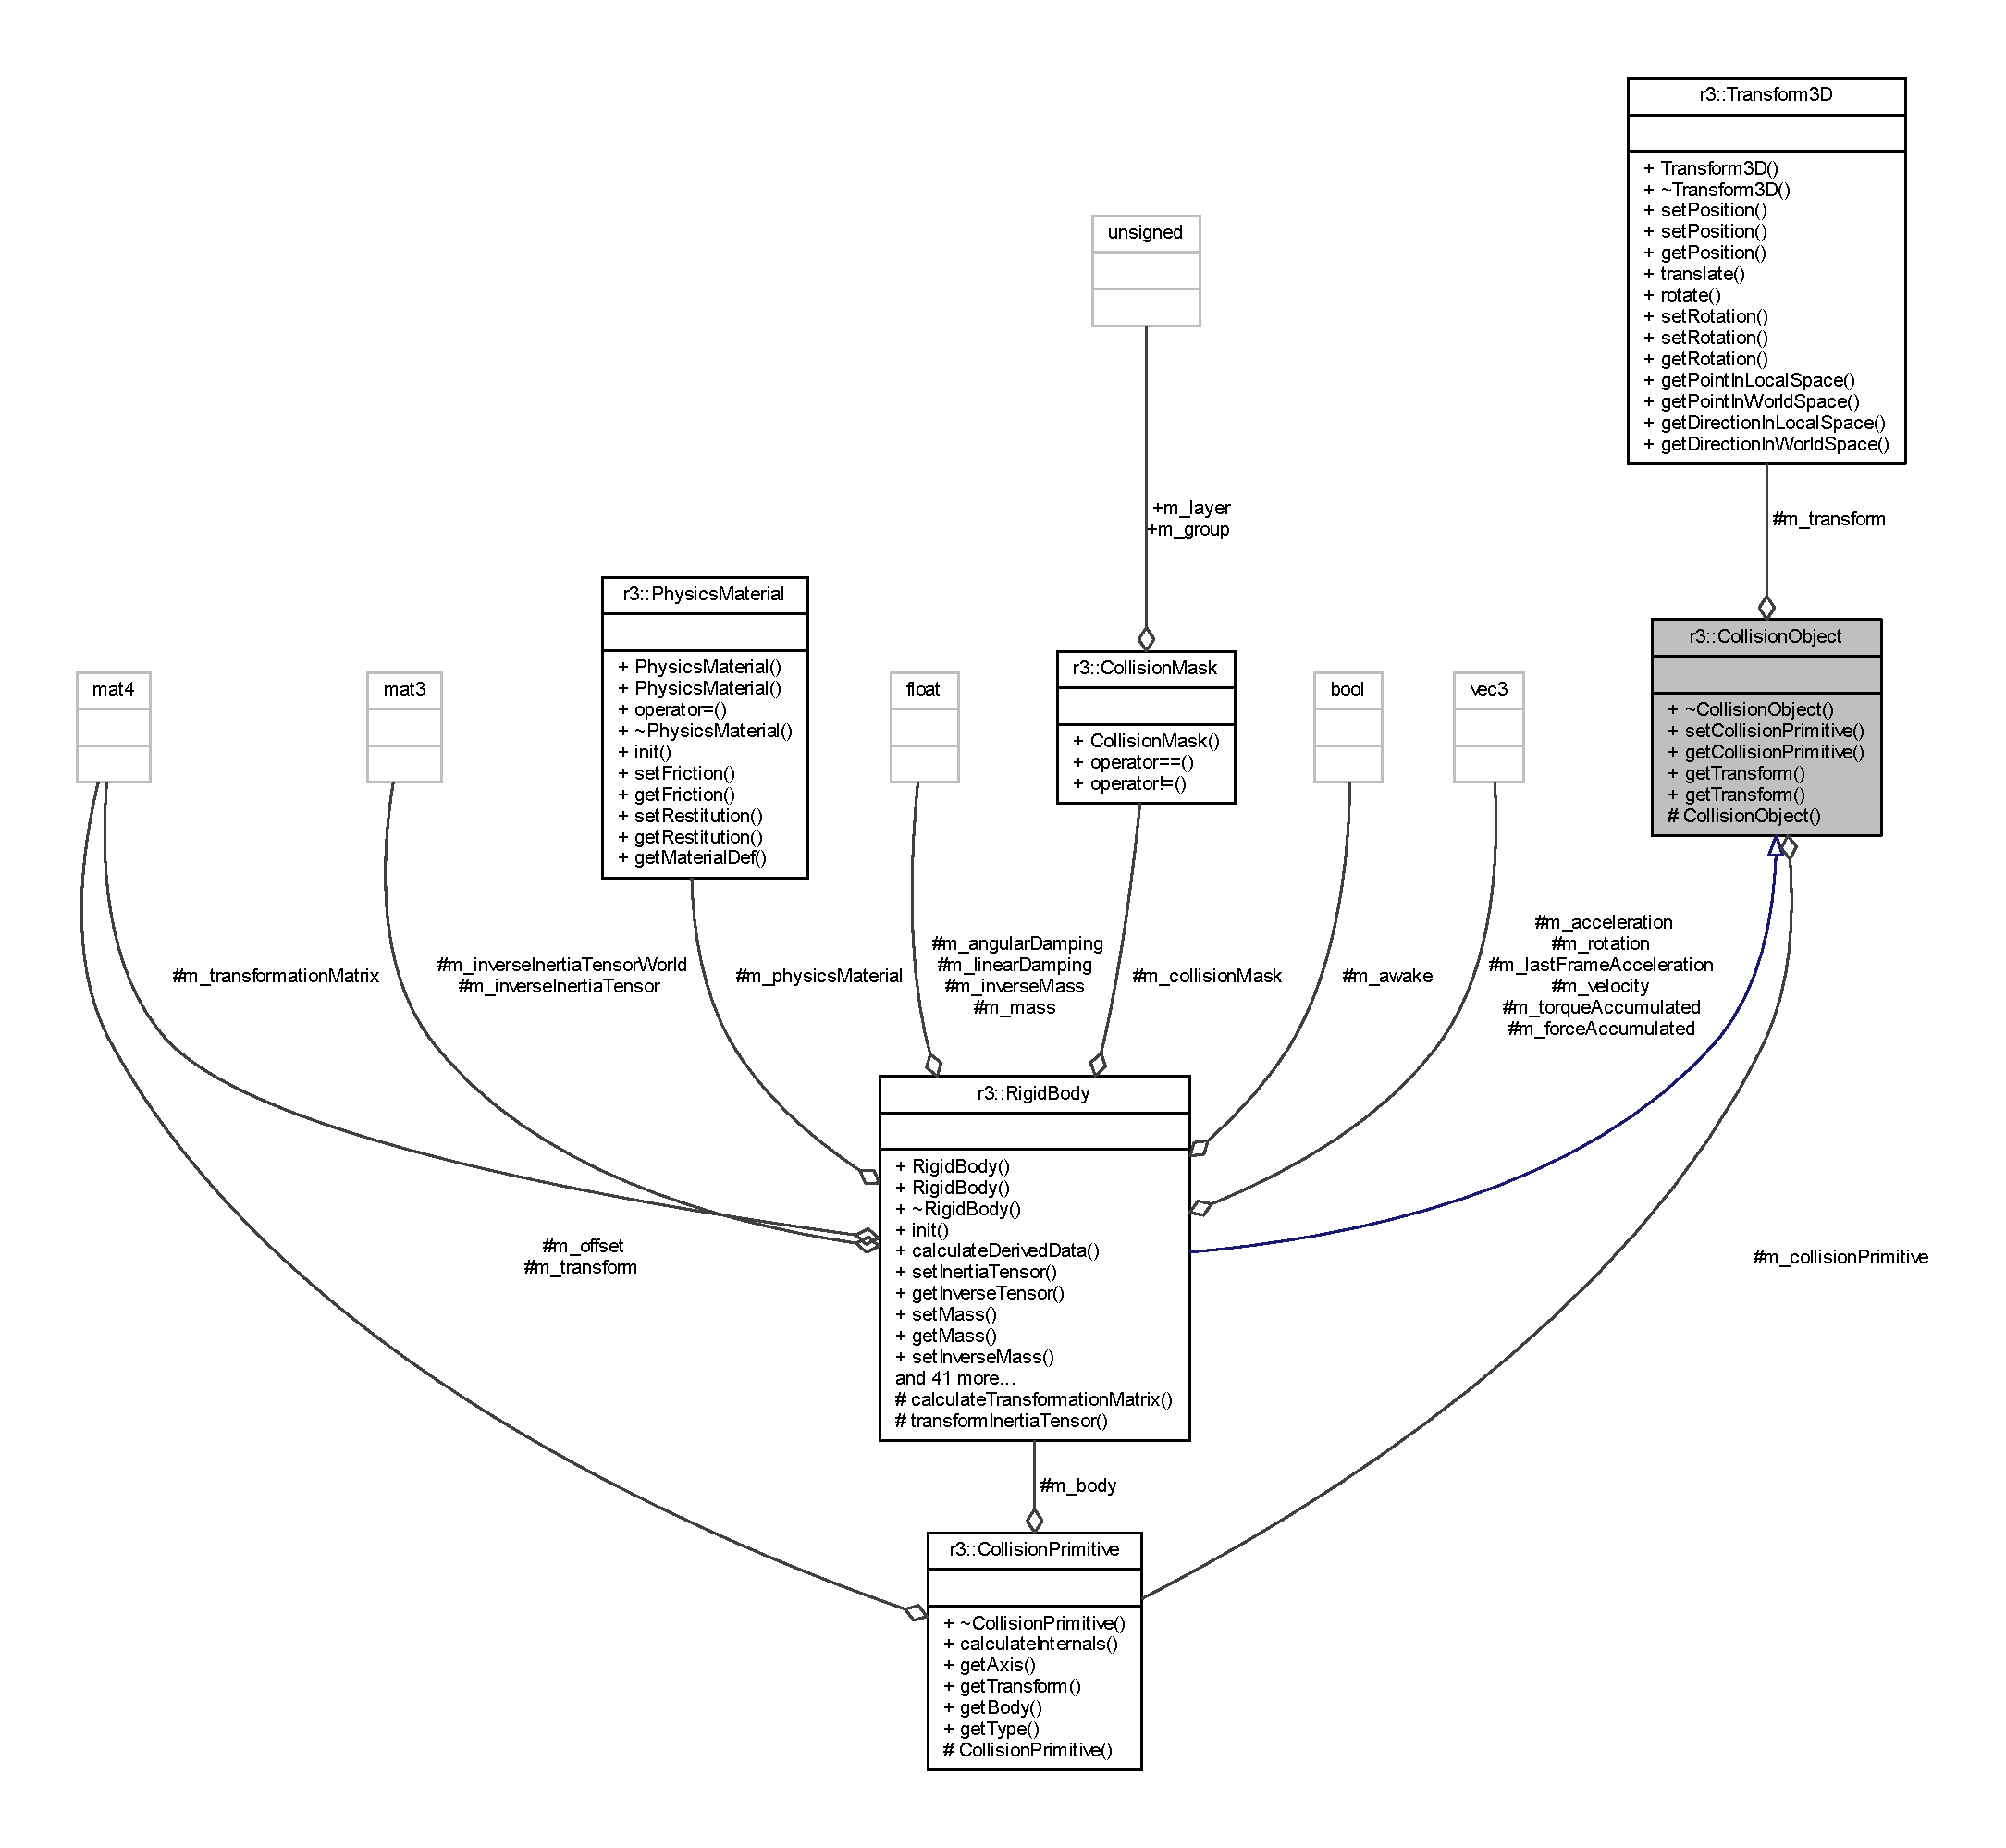
\includegraphics[width=350pt]{classr3_1_1_collision_object__coll__graph}
\end{center}
\end{figure}
\subsection*{Public Member Functions}
\begin{DoxyCompactItemize}
\item 
virtual \mbox{\hyperlink{classr3_1_1_collision_object_a26f7c8a9adb08718c98dce736cc89830}{$\sim$\+Collision\+Object}} ()
\item 
void \mbox{\hyperlink{classr3_1_1_collision_object_afaf76460298998bcbe405c0b2e6de6a6}{set\+Collision\+Primitive}} (\mbox{\hyperlink{classr3_1_1_collision_primitive}{Collision\+Primitive}} $\ast$collision\+Primitive)
\item 
\mbox{\hyperlink{classr3_1_1_collision_primitive}{Collision\+Primitive}} $\ast$ \mbox{\hyperlink{classr3_1_1_collision_object_aabb0d7173dacef5ffc02163557f55fa4}{get\+Collision\+Primitive}} () const
\item 
const \mbox{\hyperlink{classr3_1_1_transform3_d}{Transform3D}} \& \mbox{\hyperlink{classr3_1_1_collision_object_a79e04809124cad6aeb25a66f11826fee}{get\+Transform}} () const
\item 
\mbox{\hyperlink{classr3_1_1_transform3_d}{Transform3D}} \& \mbox{\hyperlink{classr3_1_1_collision_object_acc41118b9a571e5aa918644aaeda6bfa}{get\+Transform}} ()
\end{DoxyCompactItemize}
\subsection*{Protected Member Functions}
\begin{DoxyCompactItemize}
\item 
\mbox{\hyperlink{classr3_1_1_collision_object_ad664d1dd3a03f183c46c6b7ba7327cfd}{Collision\+Object}} (\mbox{\hyperlink{classr3_1_1_collision_primitive}{Collision\+Primitive}} $\ast$collision\+Primitive=nullptr)
\end{DoxyCompactItemize}
\subsection*{Protected Attributes}
\begin{DoxyCompactItemize}
\item 
\mbox{\hyperlink{classr3_1_1_collision_primitive}{Collision\+Primitive}} $\ast$ \mbox{\hyperlink{classr3_1_1_collision_object_afa62ecdda20144d43f9fcf72d56642d6}{m\+\_\+collision\+Primitive}}
\item 
\mbox{\hyperlink{classr3_1_1_transform3_d}{Transform3D}} \mbox{\hyperlink{classr3_1_1_collision_object_a2ed717150a250f1b81e23ba7e5431542}{m\+\_\+transform}}
\end{DoxyCompactItemize}


\subsection{Constructor \& Destructor Documentation}
\mbox{\Hypertarget{classr3_1_1_collision_object_a26f7c8a9adb08718c98dce736cc89830}\label{classr3_1_1_collision_object_a26f7c8a9adb08718c98dce736cc89830}} 
\index{r3\+::\+Collision\+Object@{r3\+::\+Collision\+Object}!````~Collision\+Object@{$\sim$\+Collision\+Object}}
\index{````~Collision\+Object@{$\sim$\+Collision\+Object}!r3\+::\+Collision\+Object@{r3\+::\+Collision\+Object}}
\subsubsection{\texorpdfstring{$\sim$\+Collision\+Object()}{~CollisionObject()}}
{\footnotesize\ttfamily r3\+::\+Collision\+Object\+::$\sim$\+Collision\+Object (\begin{DoxyParamCaption}{ }\end{DoxyParamCaption})\hspace{0.3cm}{\ttfamily [virtual]}, {\ttfamily [default]}}

\mbox{\Hypertarget{classr3_1_1_collision_object_ad664d1dd3a03f183c46c6b7ba7327cfd}\label{classr3_1_1_collision_object_ad664d1dd3a03f183c46c6b7ba7327cfd}} 
\index{r3\+::\+Collision\+Object@{r3\+::\+Collision\+Object}!Collision\+Object@{Collision\+Object}}
\index{Collision\+Object@{Collision\+Object}!r3\+::\+Collision\+Object@{r3\+::\+Collision\+Object}}
\subsubsection{\texorpdfstring{Collision\+Object()}{CollisionObject()}}
{\footnotesize\ttfamily r3\+::\+Collision\+Object\+::\+Collision\+Object (\begin{DoxyParamCaption}\item[{\mbox{\hyperlink{classr3_1_1_collision_primitive}{Collision\+Primitive}} $\ast$}]{collision\+Primitive = {\ttfamily nullptr} }\end{DoxyParamCaption})\hspace{0.3cm}{\ttfamily [explicit]}, {\ttfamily [protected]}}



\subsection{Member Function Documentation}
\mbox{\Hypertarget{classr3_1_1_collision_object_aabb0d7173dacef5ffc02163557f55fa4}\label{classr3_1_1_collision_object_aabb0d7173dacef5ffc02163557f55fa4}} 
\index{r3\+::\+Collision\+Object@{r3\+::\+Collision\+Object}!get\+Collision\+Primitive@{get\+Collision\+Primitive}}
\index{get\+Collision\+Primitive@{get\+Collision\+Primitive}!r3\+::\+Collision\+Object@{r3\+::\+Collision\+Object}}
\subsubsection{\texorpdfstring{get\+Collision\+Primitive()}{getCollisionPrimitive()}}
{\footnotesize\ttfamily \mbox{\hyperlink{classr3_1_1_collision_primitive}{Collision\+Primitive}} $\ast$ r3\+::\+Collision\+Object\+::get\+Collision\+Primitive (\begin{DoxyParamCaption}{ }\end{DoxyParamCaption}) const}

Get the currently used collision primitive \mbox{\Hypertarget{classr3_1_1_collision_object_a79e04809124cad6aeb25a66f11826fee}\label{classr3_1_1_collision_object_a79e04809124cad6aeb25a66f11826fee}} 
\index{r3\+::\+Collision\+Object@{r3\+::\+Collision\+Object}!get\+Transform@{get\+Transform}}
\index{get\+Transform@{get\+Transform}!r3\+::\+Collision\+Object@{r3\+::\+Collision\+Object}}
\subsubsection{\texorpdfstring{get\+Transform()}{getTransform()}\hspace{0.1cm}{\footnotesize\ttfamily [1/2]}}
{\footnotesize\ttfamily const \mbox{\hyperlink{classr3_1_1_transform3_d}{Transform3D}} \& r3\+::\+Collision\+Object\+::get\+Transform (\begin{DoxyParamCaption}{ }\end{DoxyParamCaption}) const}

\mbox{\Hypertarget{classr3_1_1_collision_object_acc41118b9a571e5aa918644aaeda6bfa}\label{classr3_1_1_collision_object_acc41118b9a571e5aa918644aaeda6bfa}} 
\index{r3\+::\+Collision\+Object@{r3\+::\+Collision\+Object}!get\+Transform@{get\+Transform}}
\index{get\+Transform@{get\+Transform}!r3\+::\+Collision\+Object@{r3\+::\+Collision\+Object}}
\subsubsection{\texorpdfstring{get\+Transform()}{getTransform()}\hspace{0.1cm}{\footnotesize\ttfamily [2/2]}}
{\footnotesize\ttfamily \mbox{\hyperlink{classr3_1_1_transform3_d}{Transform3D}} \& r3\+::\+Collision\+Object\+::get\+Transform (\begin{DoxyParamCaption}{ }\end{DoxyParamCaption})}

\mbox{\Hypertarget{classr3_1_1_collision_object_afaf76460298998bcbe405c0b2e6de6a6}\label{classr3_1_1_collision_object_afaf76460298998bcbe405c0b2e6de6a6}} 
\index{r3\+::\+Collision\+Object@{r3\+::\+Collision\+Object}!set\+Collision\+Primitive@{set\+Collision\+Primitive}}
\index{set\+Collision\+Primitive@{set\+Collision\+Primitive}!r3\+::\+Collision\+Object@{r3\+::\+Collision\+Object}}
\subsubsection{\texorpdfstring{set\+Collision\+Primitive()}{setCollisionPrimitive()}}
{\footnotesize\ttfamily void r3\+::\+Collision\+Object\+::set\+Collision\+Primitive (\begin{DoxyParamCaption}\item[{\mbox{\hyperlink{classr3_1_1_collision_primitive}{Collision\+Primitive}} $\ast$}]{collision\+Primitive }\end{DoxyParamCaption})}

Set the collision primitive used for collision detection. 

\subsection{Member Data Documentation}
\mbox{\Hypertarget{classr3_1_1_collision_object_afa62ecdda20144d43f9fcf72d56642d6}\label{classr3_1_1_collision_object_afa62ecdda20144d43f9fcf72d56642d6}} 
\index{r3\+::\+Collision\+Object@{r3\+::\+Collision\+Object}!m\+\_\+collision\+Primitive@{m\+\_\+collision\+Primitive}}
\index{m\+\_\+collision\+Primitive@{m\+\_\+collision\+Primitive}!r3\+::\+Collision\+Object@{r3\+::\+Collision\+Object}}
\subsubsection{\texorpdfstring{m\+\_\+collision\+Primitive}{m\_collisionPrimitive}}
{\footnotesize\ttfamily \mbox{\hyperlink{classr3_1_1_collision_primitive}{Collision\+Primitive}}$\ast$ r3\+::\+Collision\+Object\+::m\+\_\+collision\+Primitive\hspace{0.3cm}{\ttfamily [protected]}}

\mbox{\Hypertarget{classr3_1_1_collision_object_a2ed717150a250f1b81e23ba7e5431542}\label{classr3_1_1_collision_object_a2ed717150a250f1b81e23ba7e5431542}} 
\index{r3\+::\+Collision\+Object@{r3\+::\+Collision\+Object}!m\+\_\+transform@{m\+\_\+transform}}
\index{m\+\_\+transform@{m\+\_\+transform}!r3\+::\+Collision\+Object@{r3\+::\+Collision\+Object}}
\subsubsection{\texorpdfstring{m\+\_\+transform}{m\_transform}}
{\footnotesize\ttfamily \mbox{\hyperlink{classr3_1_1_transform3_d}{Transform3D}} r3\+::\+Collision\+Object\+::m\+\_\+transform\hspace{0.3cm}{\ttfamily [protected]}}



The documentation for this class was generated from the following files\+:\begin{DoxyCompactItemize}
\item 
D\+:/\+Library/\+Documents/\+Job/\+Forschungsmaster/\+Projekte/\+Simulation\+Visualization/\+Rumble3\+D/\+Rumble3\+D/include/\+R3\+D/\+Rigid\+Body\+Engine/\mbox{\hyperlink{_collision_object_8h}{Collision\+Object.\+h}}\item 
D\+:/\+Library/\+Documents/\+Job/\+Forschungsmaster/\+Projekte/\+Simulation\+Visualization/\+Rumble3\+D/\+Rumble3\+D/src/\+Rigid\+Body\+Engine/\mbox{\hyperlink{_collision_object_8cpp}{Collision\+Object.\+cpp}}\end{DoxyCompactItemize}

\hypertarget{structr3_1_1_collision_pair}{}\section{r3\+:\+:Collision\+Pair Struct Reference}
\label{structr3_1_1_collision_pair}\index{r3\+::\+Collision\+Pair@{r3\+::\+Collision\+Pair}}


{\ttfamily \#include $<$Collision\+Pair.\+h$>$}



Collaboration diagram for r3\+:\+:Collision\+Pair\+:\nopagebreak
\begin{figure}[H]
\begin{center}
\leavevmode
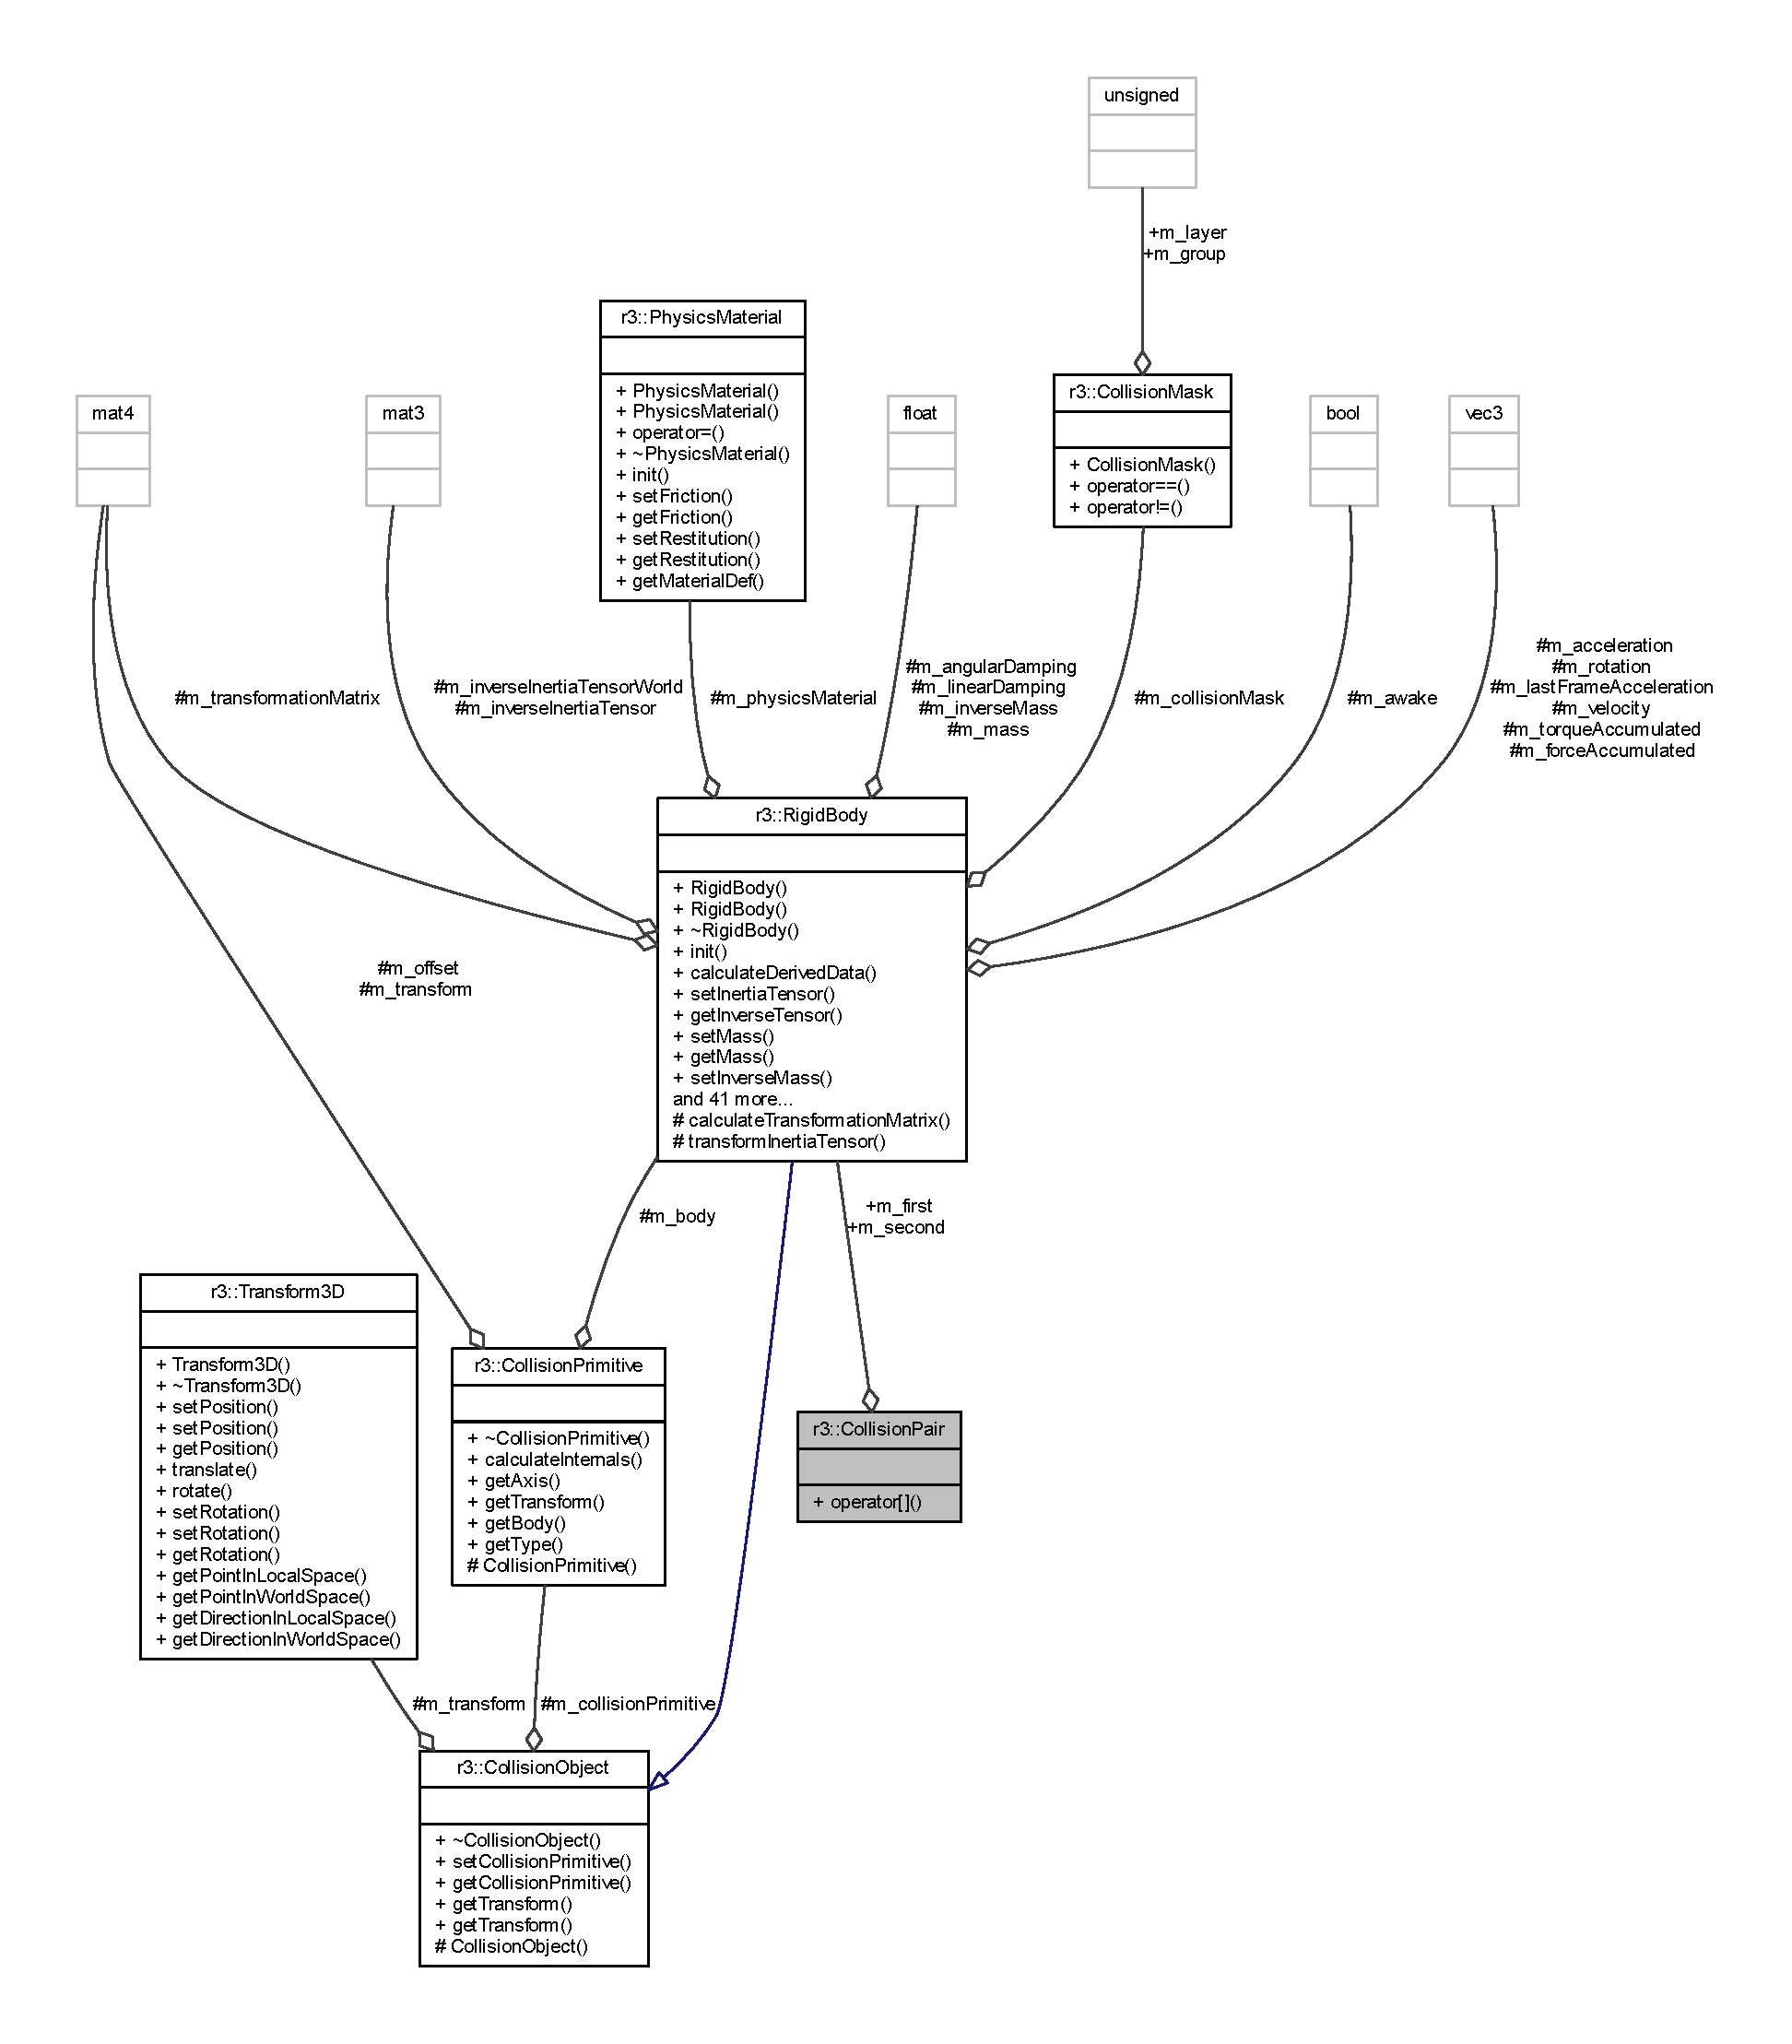
\includegraphics[width=350pt]{structr3_1_1_collision_pair__coll__graph}
\end{center}
\end{figure}
\subsection*{Public Member Functions}
\begin{DoxyCompactItemize}
\item 
\mbox{\hyperlink{classr3_1_1_rigid_body}{Rigid\+Body}} $\ast$ \mbox{\hyperlink{structr3_1_1_collision_pair_ae6b965e4d3525253b9b1e3270e8665e8}{operator\mbox{[}$\,$\mbox{]}}} (const int index)
\end{DoxyCompactItemize}
\subsection*{Public Attributes}
\begin{DoxyCompactItemize}
\item 
\mbox{\hyperlink{classr3_1_1_rigid_body}{Rigid\+Body}} $\ast$ \mbox{\hyperlink{structr3_1_1_collision_pair_a6c2fbf8e05b333a4e93f6ac75049d429}{m\+\_\+first}}
\item 
\mbox{\hyperlink{classr3_1_1_rigid_body}{Rigid\+Body}} $\ast$ \mbox{\hyperlink{structr3_1_1_collision_pair_ad7ff97123502a1e0535d3f5da8013411}{m\+\_\+second}}
\end{DoxyCompactItemize}


\subsection{Member Function Documentation}
\mbox{\Hypertarget{structr3_1_1_collision_pair_ae6b965e4d3525253b9b1e3270e8665e8}\label{structr3_1_1_collision_pair_ae6b965e4d3525253b9b1e3270e8665e8}} 
\index{r3\+::\+Collision\+Pair@{r3\+::\+Collision\+Pair}!operator\mbox{[}\mbox{]}@{operator[]}}
\index{operator\mbox{[}\mbox{]}@{operator[]}!r3\+::\+Collision\+Pair@{r3\+::\+Collision\+Pair}}
\subsubsection{\texorpdfstring{operator[]()}{operator[]()}}
{\footnotesize\ttfamily \mbox{\hyperlink{classr3_1_1_rigid_body}{Rigid\+Body}}$\ast$ r3\+::\+Collision\+Pair\+::operator\mbox{[}$\,$\mbox{]} (\begin{DoxyParamCaption}\item[{const int}]{index }\end{DoxyParamCaption})\hspace{0.3cm}{\ttfamily [inline]}}



\subsection{Member Data Documentation}
\mbox{\Hypertarget{structr3_1_1_collision_pair_a6c2fbf8e05b333a4e93f6ac75049d429}\label{structr3_1_1_collision_pair_a6c2fbf8e05b333a4e93f6ac75049d429}} 
\index{r3\+::\+Collision\+Pair@{r3\+::\+Collision\+Pair}!m\+\_\+first@{m\+\_\+first}}
\index{m\+\_\+first@{m\+\_\+first}!r3\+::\+Collision\+Pair@{r3\+::\+Collision\+Pair}}
\subsubsection{\texorpdfstring{m\+\_\+first}{m\_first}}
{\footnotesize\ttfamily \mbox{\hyperlink{classr3_1_1_rigid_body}{Rigid\+Body}}$\ast$ r3\+::\+Collision\+Pair\+::m\+\_\+first}

\mbox{\Hypertarget{structr3_1_1_collision_pair_ad7ff97123502a1e0535d3f5da8013411}\label{structr3_1_1_collision_pair_ad7ff97123502a1e0535d3f5da8013411}} 
\index{r3\+::\+Collision\+Pair@{r3\+::\+Collision\+Pair}!m\+\_\+second@{m\+\_\+second}}
\index{m\+\_\+second@{m\+\_\+second}!r3\+::\+Collision\+Pair@{r3\+::\+Collision\+Pair}}
\subsubsection{\texorpdfstring{m\+\_\+second}{m\_second}}
{\footnotesize\ttfamily \mbox{\hyperlink{classr3_1_1_rigid_body}{Rigid\+Body}}$\ast$ r3\+::\+Collision\+Pair\+::m\+\_\+second}



The documentation for this struct was generated from the following file\+:\begin{DoxyCompactItemize}
\item 
D\+:/\+Library/\+Documents/\+Job/\+Forschungsmaster/\+Projekte/\+Simulation\+Visualization/\+Rumble3\+D/\+Rumble3\+D/include/\+R3\+D/\+Rigid\+Body\+Engine/\+Collision\+Detection/\mbox{\hyperlink{_collision_pair_8h}{Collision\+Pair.\+h}}\end{DoxyCompactItemize}

\hypertarget{classr3_1_1_collision_plane}{}\section{r3\+:\+:Collision\+Plane Class Reference}
\label{classr3_1_1_collision_plane}\index{r3\+::\+Collision\+Plane@{r3\+::\+Collision\+Plane}}


{\ttfamily \#include $<$Collision\+Plane.\+h$>$}



Inheritance diagram for r3\+:\+:Collision\+Plane\+:\nopagebreak
\begin{figure}[H]
\begin{center}
\leavevmode
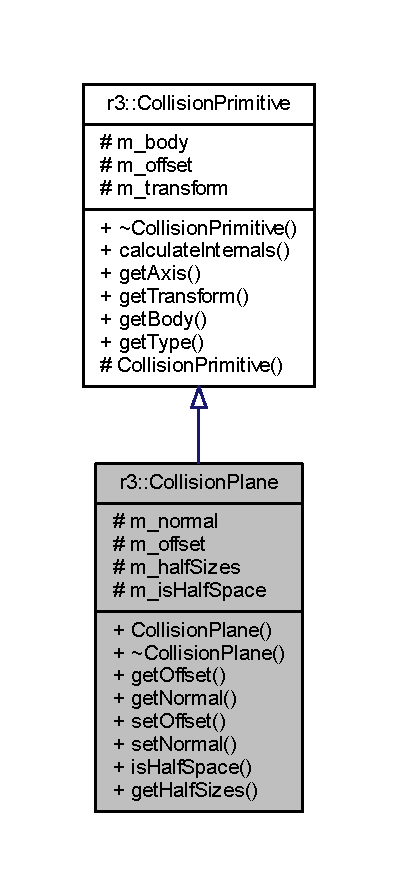
\includegraphics[width=191pt]{classr3_1_1_collision_plane__inherit__graph}
\end{center}
\end{figure}


Collaboration diagram for r3\+:\+:Collision\+Plane\+:\nopagebreak
\begin{figure}[H]
\begin{center}
\leavevmode
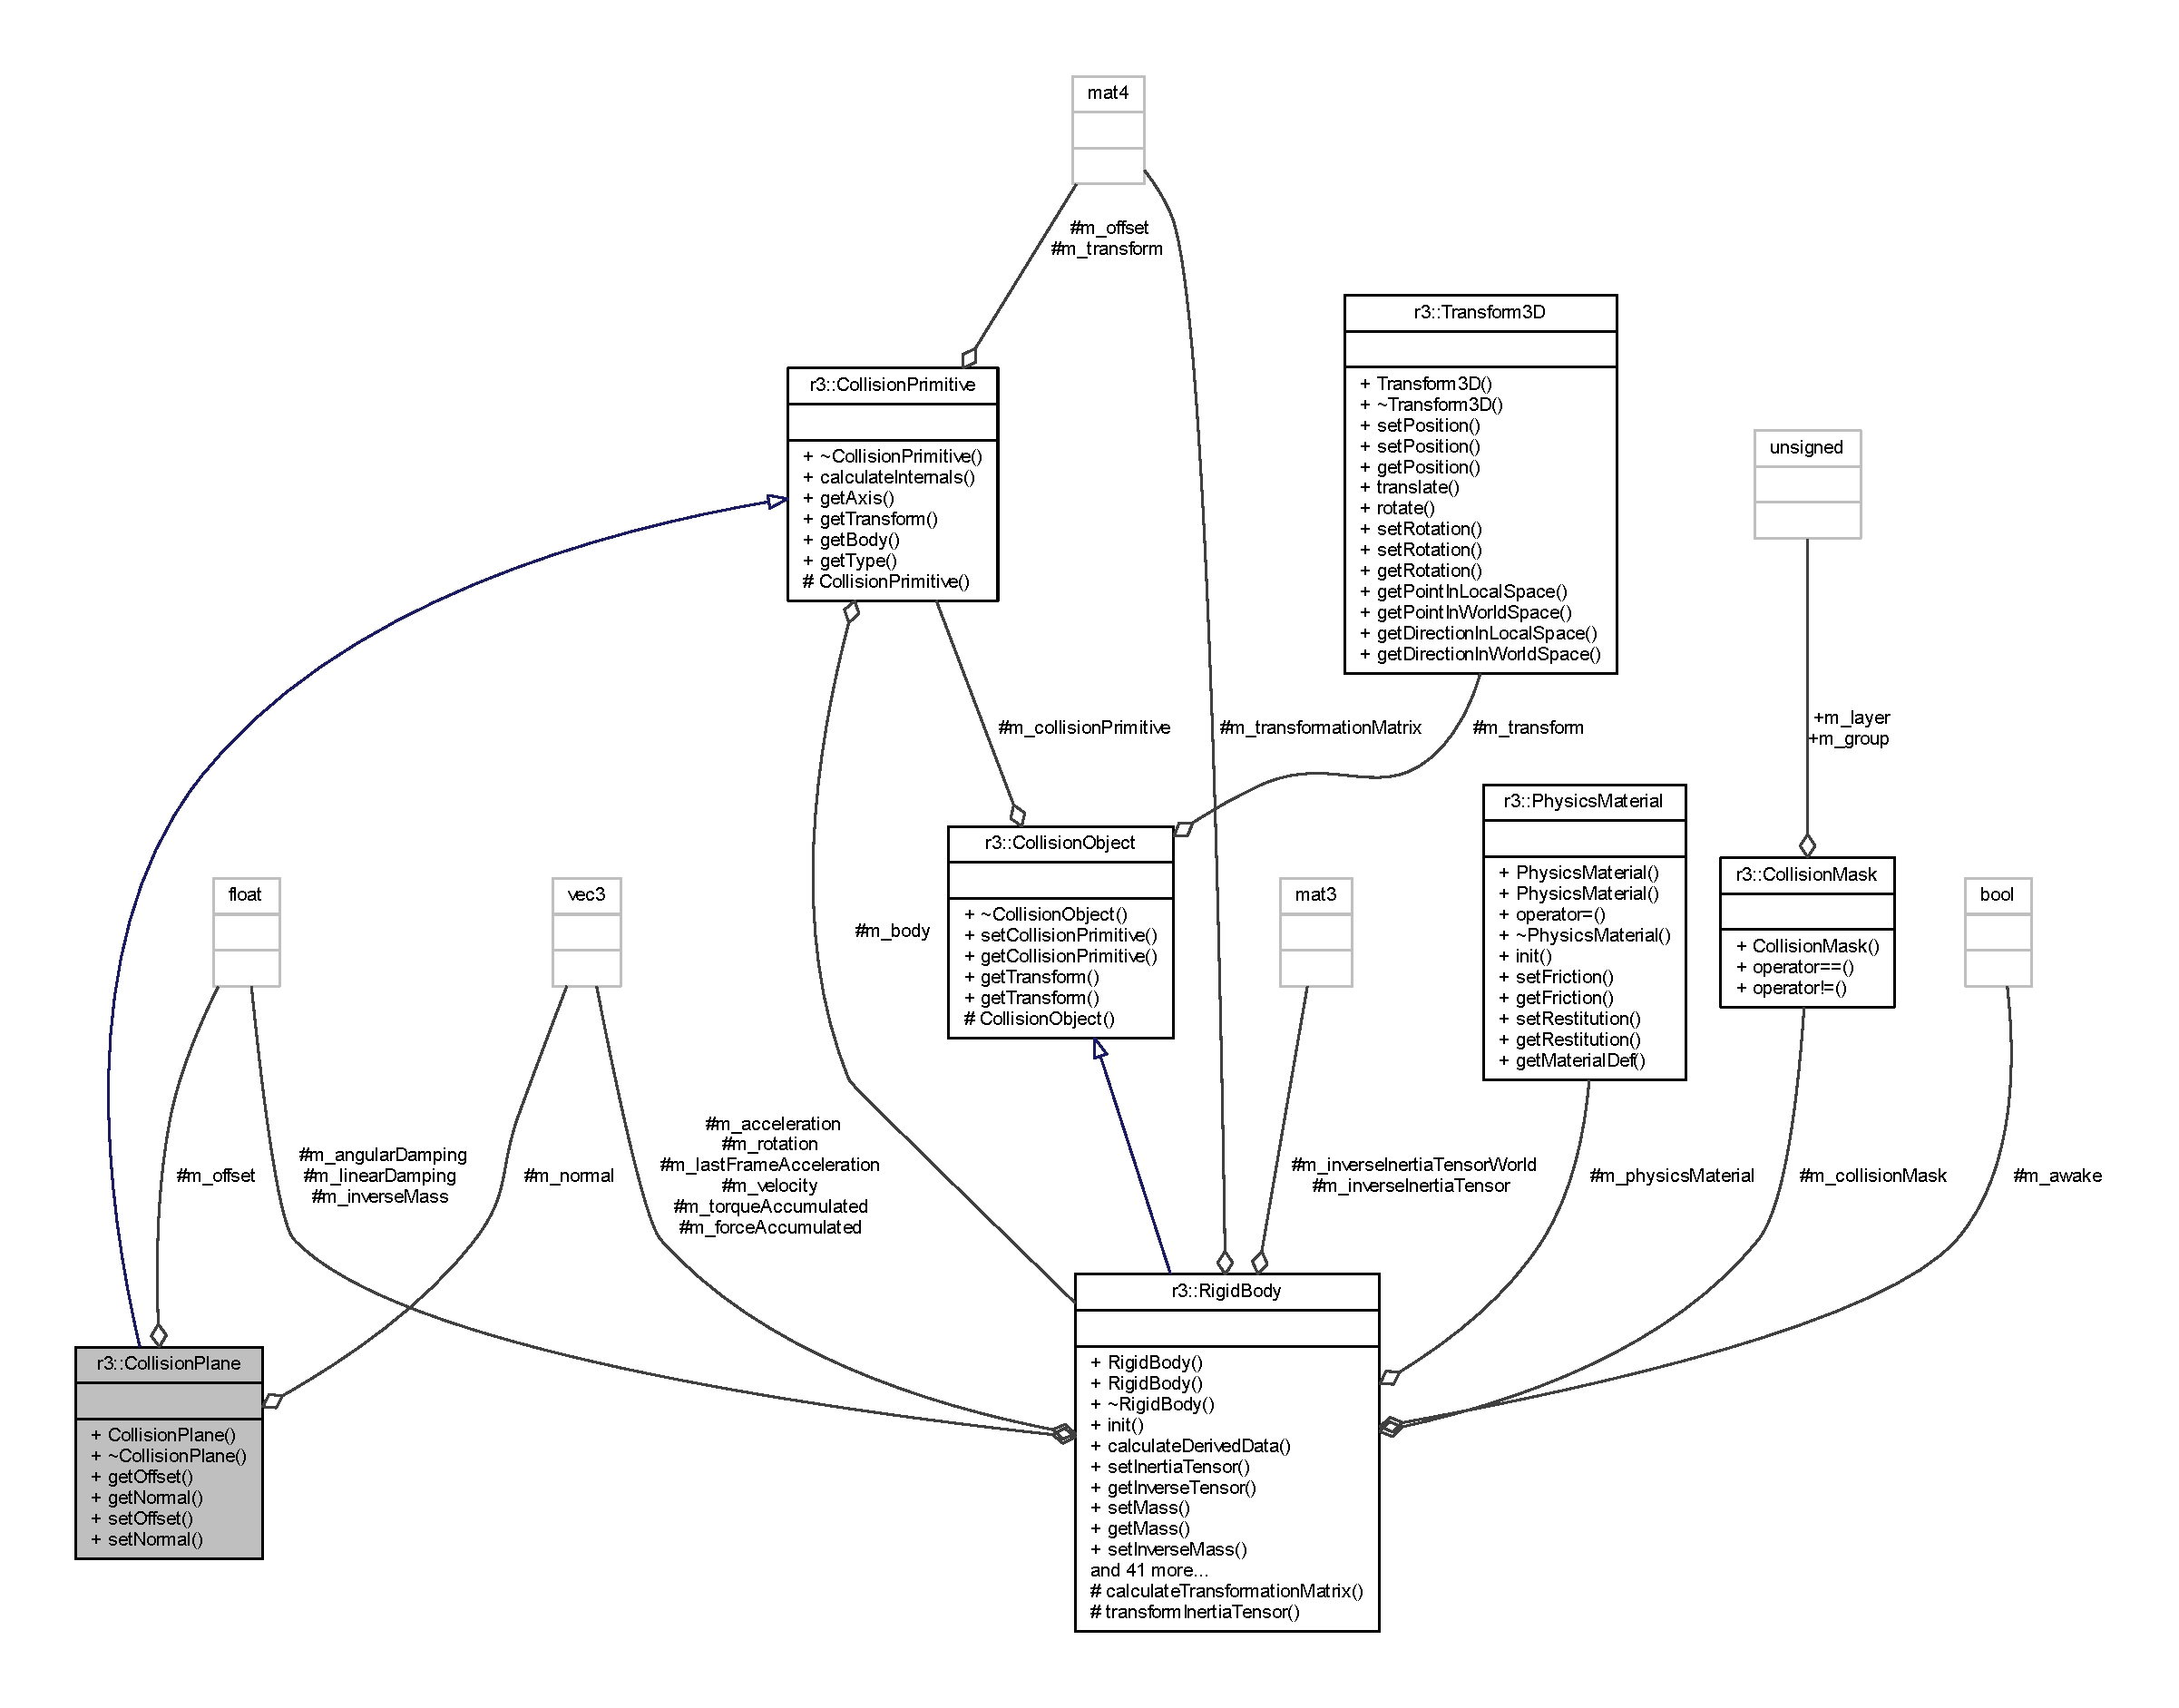
\includegraphics[width=350pt]{classr3_1_1_collision_plane__coll__graph}
\end{center}
\end{figure}
\subsection*{Public Member Functions}
\begin{DoxyCompactItemize}
\item 
\mbox{\hyperlink{classr3_1_1_collision_plane_ae3f8642b62667018e4a4c3120880fd0f}{Collision\+Plane}} (const glm\+::vec3 \&normal, \mbox{\hyperlink{namespacer3_ab2016b3e3f743fb735afce242f0dc1eb}{real}} offset, const glm\+::vec2 \&half\+Sizes=glm\+::vec2(1.\+0f, 1.\+0f), bool is\+Half\+Space=false)
\item 
\mbox{\hyperlink{classr3_1_1_collision_plane_a4c83b51c544a5fda9d949baced5cea02}{$\sim$\+Collision\+Plane}} ()
\item 
\mbox{\hyperlink{namespacer3_ab2016b3e3f743fb735afce242f0dc1eb}{real}} \mbox{\hyperlink{classr3_1_1_collision_plane_a62e2b4bd6a811f8d2541329cd9a49bf8}{get\+Offset}} () const
\item 
glm\+::vec3 \mbox{\hyperlink{classr3_1_1_collision_plane_aa6605acf447da4e45084e6d25c1067ad}{get\+Normal}} () const
\item 
void \mbox{\hyperlink{classr3_1_1_collision_plane_ae37e09e6b807cdd800671daa5623b073}{set\+Offset}} (\mbox{\hyperlink{namespacer3_ab2016b3e3f743fb735afce242f0dc1eb}{real}} offset)
\item 
void \mbox{\hyperlink{classr3_1_1_collision_plane_a1fa140b6648f14bef9720ac0d4eefc99}{set\+Normal}} (const glm\+::vec3 \&normal)
\item 
bool \mbox{\hyperlink{classr3_1_1_collision_plane_a87f5071d181b4c643b42cb2448464be2}{is\+Half\+Space}} () const
\item 
const glm\+::vec2 \& \mbox{\hyperlink{classr3_1_1_collision_plane_ab48030fbf5bc17cd5ad81e5eb654a4b4}{get\+Half\+Sizes}} () const
\end{DoxyCompactItemize}
\subsection*{Protected Attributes}
\begin{DoxyCompactItemize}
\item 
glm\+::vec3 \mbox{\hyperlink{classr3_1_1_collision_plane_ab65e832434d2da433e79c93ac12f4b43}{m\+\_\+normal}}
\item 
\mbox{\hyperlink{namespacer3_ab2016b3e3f743fb735afce242f0dc1eb}{real}} \mbox{\hyperlink{classr3_1_1_collision_plane_a8ae3c28197b05088e405ff9944632f74}{m\+\_\+offset}}
\item 
glm\+::vec2 \mbox{\hyperlink{classr3_1_1_collision_plane_a8e642d9075ceebd029f3869ace65dd5f}{m\+\_\+half\+Sizes}}
\item 
bool \mbox{\hyperlink{classr3_1_1_collision_plane_a6d560c5f7627efec1d094905ec4e7d60}{m\+\_\+is\+Half\+Space}}
\end{DoxyCompactItemize}
\subsection*{Additional Inherited Members}


\subsection{Constructor \& Destructor Documentation}
\mbox{\Hypertarget{classr3_1_1_collision_plane_ae3f8642b62667018e4a4c3120880fd0f}\label{classr3_1_1_collision_plane_ae3f8642b62667018e4a4c3120880fd0f}} 
\index{r3\+::\+Collision\+Plane@{r3\+::\+Collision\+Plane}!Collision\+Plane@{Collision\+Plane}}
\index{Collision\+Plane@{Collision\+Plane}!r3\+::\+Collision\+Plane@{r3\+::\+Collision\+Plane}}
\subsubsection{\texorpdfstring{Collision\+Plane()}{CollisionPlane()}}
{\footnotesize\ttfamily r3\+::\+Collision\+Plane\+::\+Collision\+Plane (\begin{DoxyParamCaption}\item[{const glm\+::vec3 \&}]{normal,  }\item[{\mbox{\hyperlink{namespacer3_ab2016b3e3f743fb735afce242f0dc1eb}{real}}}]{offset,  }\item[{const glm\+::vec2 \&}]{half\+Sizes = {\ttfamily glm\+:\+:vec2(1.0f,~1.0f)},  }\item[{bool}]{is\+Half\+Space = {\ttfamily false} }\end{DoxyParamCaption})}

\mbox{\Hypertarget{classr3_1_1_collision_plane_a4c83b51c544a5fda9d949baced5cea02}\label{classr3_1_1_collision_plane_a4c83b51c544a5fda9d949baced5cea02}} 
\index{r3\+::\+Collision\+Plane@{r3\+::\+Collision\+Plane}!````~Collision\+Plane@{$\sim$\+Collision\+Plane}}
\index{````~Collision\+Plane@{$\sim$\+Collision\+Plane}!r3\+::\+Collision\+Plane@{r3\+::\+Collision\+Plane}}
\subsubsection{\texorpdfstring{$\sim$\+Collision\+Plane()}{~CollisionPlane()}}
{\footnotesize\ttfamily r3\+::\+Collision\+Plane\+::$\sim$\+Collision\+Plane (\begin{DoxyParamCaption}{ }\end{DoxyParamCaption})\hspace{0.3cm}{\ttfamily [default]}}



\subsection{Member Function Documentation}
\mbox{\Hypertarget{classr3_1_1_collision_plane_ab48030fbf5bc17cd5ad81e5eb654a4b4}\label{classr3_1_1_collision_plane_ab48030fbf5bc17cd5ad81e5eb654a4b4}} 
\index{r3\+::\+Collision\+Plane@{r3\+::\+Collision\+Plane}!get\+Half\+Sizes@{get\+Half\+Sizes}}
\index{get\+Half\+Sizes@{get\+Half\+Sizes}!r3\+::\+Collision\+Plane@{r3\+::\+Collision\+Plane}}
\subsubsection{\texorpdfstring{get\+Half\+Sizes()}{getHalfSizes()}}
{\footnotesize\ttfamily const glm\+::vec2 \& r3\+::\+Collision\+Plane\+::get\+Half\+Sizes (\begin{DoxyParamCaption}{ }\end{DoxyParamCaption}) const}

Get scaling in x-\/z directions \mbox{\Hypertarget{classr3_1_1_collision_plane_aa6605acf447da4e45084e6d25c1067ad}\label{classr3_1_1_collision_plane_aa6605acf447da4e45084e6d25c1067ad}} 
\index{r3\+::\+Collision\+Plane@{r3\+::\+Collision\+Plane}!get\+Normal@{get\+Normal}}
\index{get\+Normal@{get\+Normal}!r3\+::\+Collision\+Plane@{r3\+::\+Collision\+Plane}}
\subsubsection{\texorpdfstring{get\+Normal()}{getNormal()}}
{\footnotesize\ttfamily glm\+::vec3 r3\+::\+Collision\+Plane\+::get\+Normal (\begin{DoxyParamCaption}{ }\end{DoxyParamCaption}) const}

\mbox{\Hypertarget{classr3_1_1_collision_plane_a62e2b4bd6a811f8d2541329cd9a49bf8}\label{classr3_1_1_collision_plane_a62e2b4bd6a811f8d2541329cd9a49bf8}} 
\index{r3\+::\+Collision\+Plane@{r3\+::\+Collision\+Plane}!get\+Offset@{get\+Offset}}
\index{get\+Offset@{get\+Offset}!r3\+::\+Collision\+Plane@{r3\+::\+Collision\+Plane}}
\subsubsection{\texorpdfstring{get\+Offset()}{getOffset()}}
{\footnotesize\ttfamily \mbox{\hyperlink{namespacer3_ab2016b3e3f743fb735afce242f0dc1eb}{real}} r3\+::\+Collision\+Plane\+::get\+Offset (\begin{DoxyParamCaption}{ }\end{DoxyParamCaption}) const}

\mbox{\Hypertarget{classr3_1_1_collision_plane_a87f5071d181b4c643b42cb2448464be2}\label{classr3_1_1_collision_plane_a87f5071d181b4c643b42cb2448464be2}} 
\index{r3\+::\+Collision\+Plane@{r3\+::\+Collision\+Plane}!is\+Half\+Space@{is\+Half\+Space}}
\index{is\+Half\+Space@{is\+Half\+Space}!r3\+::\+Collision\+Plane@{r3\+::\+Collision\+Plane}}
\subsubsection{\texorpdfstring{is\+Half\+Space()}{isHalfSpace()}}
{\footnotesize\ttfamily bool r3\+::\+Collision\+Plane\+::is\+Half\+Space (\begin{DoxyParamCaption}{ }\end{DoxyParamCaption}) const}

Check if this plane defines a half space. If this is the case, the normal will point away from this half space. \mbox{\Hypertarget{classr3_1_1_collision_plane_a1fa140b6648f14bef9720ac0d4eefc99}\label{classr3_1_1_collision_plane_a1fa140b6648f14bef9720ac0d4eefc99}} 
\index{r3\+::\+Collision\+Plane@{r3\+::\+Collision\+Plane}!set\+Normal@{set\+Normal}}
\index{set\+Normal@{set\+Normal}!r3\+::\+Collision\+Plane@{r3\+::\+Collision\+Plane}}
\subsubsection{\texorpdfstring{set\+Normal()}{setNormal()}}
{\footnotesize\ttfamily void r3\+::\+Collision\+Plane\+::set\+Normal (\begin{DoxyParamCaption}\item[{const glm\+::vec3 \&}]{normal }\end{DoxyParamCaption})}

\mbox{\Hypertarget{classr3_1_1_collision_plane_ae37e09e6b807cdd800671daa5623b073}\label{classr3_1_1_collision_plane_ae37e09e6b807cdd800671daa5623b073}} 
\index{r3\+::\+Collision\+Plane@{r3\+::\+Collision\+Plane}!set\+Offset@{set\+Offset}}
\index{set\+Offset@{set\+Offset}!r3\+::\+Collision\+Plane@{r3\+::\+Collision\+Plane}}
\subsubsection{\texorpdfstring{set\+Offset()}{setOffset()}}
{\footnotesize\ttfamily void r3\+::\+Collision\+Plane\+::set\+Offset (\begin{DoxyParamCaption}\item[{\mbox{\hyperlink{namespacer3_ab2016b3e3f743fb735afce242f0dc1eb}{real}}}]{offset }\end{DoxyParamCaption})}



\subsection{Member Data Documentation}
\mbox{\Hypertarget{classr3_1_1_collision_plane_a8e642d9075ceebd029f3869ace65dd5f}\label{classr3_1_1_collision_plane_a8e642d9075ceebd029f3869ace65dd5f}} 
\index{r3\+::\+Collision\+Plane@{r3\+::\+Collision\+Plane}!m\+\_\+half\+Sizes@{m\+\_\+half\+Sizes}}
\index{m\+\_\+half\+Sizes@{m\+\_\+half\+Sizes}!r3\+::\+Collision\+Plane@{r3\+::\+Collision\+Plane}}
\subsubsection{\texorpdfstring{m\+\_\+half\+Sizes}{m\_halfSizes}}
{\footnotesize\ttfamily glm\+::vec2 r3\+::\+Collision\+Plane\+::m\+\_\+half\+Sizes\hspace{0.3cm}{\ttfamily [protected]}}

\mbox{\Hypertarget{classr3_1_1_collision_plane_a6d560c5f7627efec1d094905ec4e7d60}\label{classr3_1_1_collision_plane_a6d560c5f7627efec1d094905ec4e7d60}} 
\index{r3\+::\+Collision\+Plane@{r3\+::\+Collision\+Plane}!m\+\_\+is\+Half\+Space@{m\+\_\+is\+Half\+Space}}
\index{m\+\_\+is\+Half\+Space@{m\+\_\+is\+Half\+Space}!r3\+::\+Collision\+Plane@{r3\+::\+Collision\+Plane}}
\subsubsection{\texorpdfstring{m\+\_\+is\+Half\+Space}{m\_isHalfSpace}}
{\footnotesize\ttfamily bool r3\+::\+Collision\+Plane\+::m\+\_\+is\+Half\+Space\hspace{0.3cm}{\ttfamily [protected]}}

\mbox{\Hypertarget{classr3_1_1_collision_plane_ab65e832434d2da433e79c93ac12f4b43}\label{classr3_1_1_collision_plane_ab65e832434d2da433e79c93ac12f4b43}} 
\index{r3\+::\+Collision\+Plane@{r3\+::\+Collision\+Plane}!m\+\_\+normal@{m\+\_\+normal}}
\index{m\+\_\+normal@{m\+\_\+normal}!r3\+::\+Collision\+Plane@{r3\+::\+Collision\+Plane}}
\subsubsection{\texorpdfstring{m\+\_\+normal}{m\_normal}}
{\footnotesize\ttfamily glm\+::vec3 r3\+::\+Collision\+Plane\+::m\+\_\+normal\hspace{0.3cm}{\ttfamily [protected]}}

\mbox{\Hypertarget{classr3_1_1_collision_plane_a8ae3c28197b05088e405ff9944632f74}\label{classr3_1_1_collision_plane_a8ae3c28197b05088e405ff9944632f74}} 
\index{r3\+::\+Collision\+Plane@{r3\+::\+Collision\+Plane}!m\+\_\+offset@{m\+\_\+offset}}
\index{m\+\_\+offset@{m\+\_\+offset}!r3\+::\+Collision\+Plane@{r3\+::\+Collision\+Plane}}
\subsubsection{\texorpdfstring{m\+\_\+offset}{m\_offset}}
{\footnotesize\ttfamily \mbox{\hyperlink{namespacer3_ab2016b3e3f743fb735afce242f0dc1eb}{real}} r3\+::\+Collision\+Plane\+::m\+\_\+offset\hspace{0.3cm}{\ttfamily [protected]}}



The documentation for this class was generated from the following files\+:\begin{DoxyCompactItemize}
\item 
D\+:/\+Job/\+Forschungsmaster/\+Projekte/\+Simulation\+Visualization/\+Rumble3\+D/\+Rumble3\+D/include/\+R3\+D/\+Rigid\+Body\+Engine/\mbox{\hyperlink{_collision_plane_8h}{Collision\+Plane.\+h}}\item 
D\+:/\+Job/\+Forschungsmaster/\+Projekte/\+Simulation\+Visualization/\+Rumble3\+D/\+Rumble3\+D/src/\+Rigid\+Body\+Engine/\mbox{\hyperlink{_collision_plane_8cpp}{Collision\+Plane.\+cpp}}\end{DoxyCompactItemize}

\hypertarget{classr3_1_1_collision_primitive}{}\section{r3\+:\+:Collision\+Primitive Class Reference}
\label{classr3_1_1_collision_primitive}\index{r3\+::\+Collision\+Primitive@{r3\+::\+Collision\+Primitive}}


{\ttfamily \#include $<$Collision\+Primitive.\+h$>$}



Inheritance diagram for r3\+:\+:Collision\+Primitive\+:\nopagebreak
\begin{figure}[H]
\begin{center}
\leavevmode
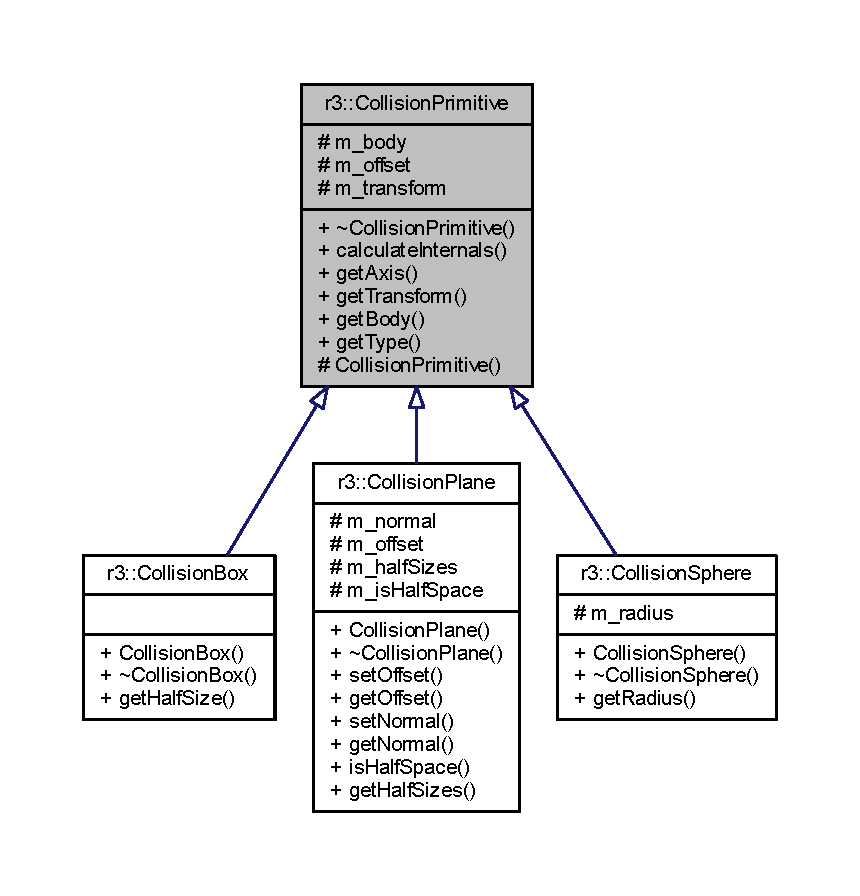
\includegraphics[width=350pt]{classr3_1_1_collision_primitive__inherit__graph}
\end{center}
\end{figure}


Collaboration diagram for r3\+:\+:Collision\+Primitive\+:\nopagebreak
\begin{figure}[H]
\begin{center}
\leavevmode
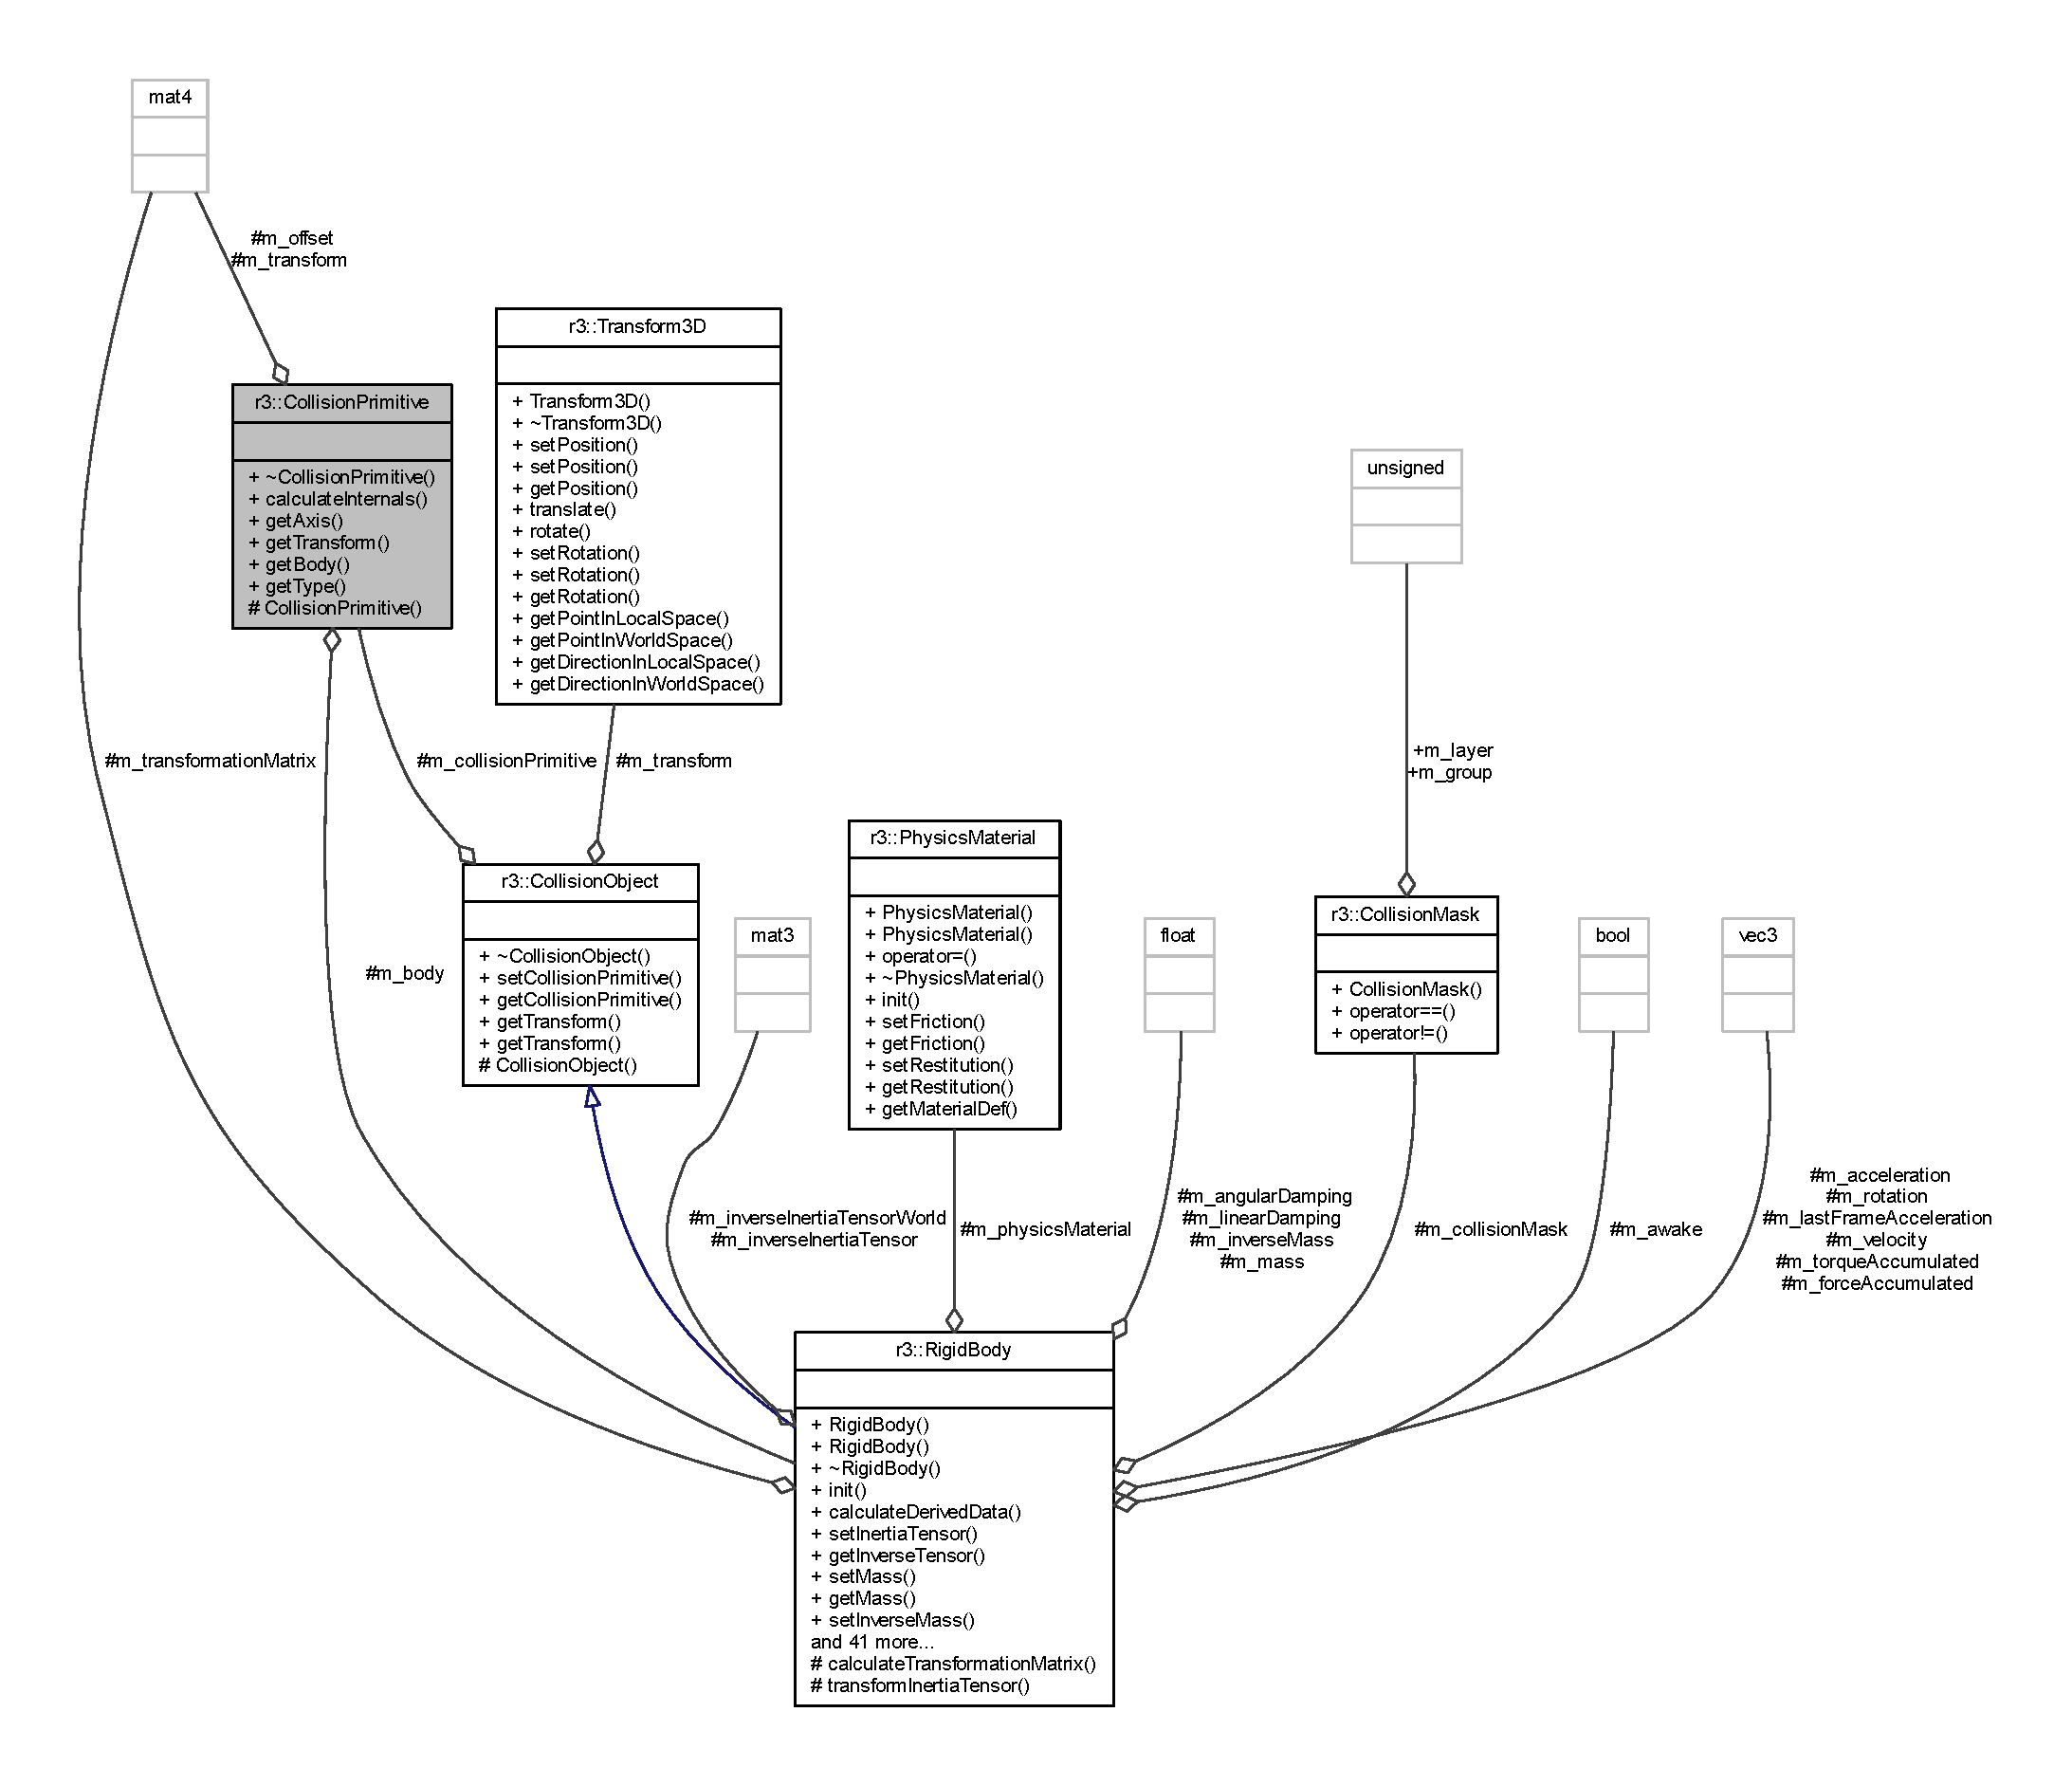
\includegraphics[width=350pt]{classr3_1_1_collision_primitive__coll__graph}
\end{center}
\end{figure}
\subsection*{Public Member Functions}
\begin{DoxyCompactItemize}
\item 
virtual \mbox{\hyperlink{classr3_1_1_collision_primitive_adfa75f14067cb33a3f0049895a3db880}{$\sim$\+Collision\+Primitive}} ()
\item 
void \mbox{\hyperlink{classr3_1_1_collision_primitive_ae27cb70a6812491c2d8de97f22c07ac6}{calculate\+Internals}} ()
\item 
glm\+::vec3 \mbox{\hyperlink{classr3_1_1_collision_primitive_a78c959f5ca0a09a0fc2038ac7f30e45a}{get\+Axis}} (unsigned index) const
\item 
const glm\+::mat4 \& \mbox{\hyperlink{classr3_1_1_collision_primitive_acc4e2139c698bab280338db36d7cc586}{get\+Transform}} () const
\item 
\mbox{\hyperlink{classr3_1_1_rigid_body}{Rigid\+Body}} $\ast$ \mbox{\hyperlink{classr3_1_1_collision_primitive_af8dbda90cce34a6262309cbdb75feea7}{get\+Body}} () const
\item 
\mbox{\hyperlink{namespacer3_a7079ec5e42c1a55140d3bc093d49e319}{Collision\+Primitive\+Type}} \mbox{\hyperlink{classr3_1_1_collision_primitive_ac7a318fb788d1442e7d3390c8e465e14}{get\+Type}} () const
\end{DoxyCompactItemize}
\subsection*{Protected Member Functions}
\begin{DoxyCompactItemize}
\item 
\mbox{\hyperlink{classr3_1_1_collision_primitive_a56f4cef84fcb4d92b0ced2ffcefdb22a}{Collision\+Primitive}} (\mbox{\hyperlink{namespacer3_a7079ec5e42c1a55140d3bc093d49e319}{Collision\+Primitive\+Type}} type)
\end{DoxyCompactItemize}
\subsection*{Protected Attributes}
\begin{DoxyCompactItemize}
\item 
\mbox{\hyperlink{classr3_1_1_rigid_body}{Rigid\+Body}} $\ast$ \mbox{\hyperlink{classr3_1_1_collision_primitive_a3ae500c9bd222ec42d86696702e746db}{m\+\_\+body}} \{\}
\item 
glm\+::mat4 \mbox{\hyperlink{classr3_1_1_collision_primitive_a15a51c2e72a8c5122a1031d6620a2901}{m\+\_\+offset}}
\item 
glm\+::mat4 \mbox{\hyperlink{classr3_1_1_collision_primitive_a0cb28517e7791b9836a5cac5d8550b13}{m\+\_\+transform}}
\end{DoxyCompactItemize}


\subsection{Constructor \& Destructor Documentation}
\mbox{\Hypertarget{classr3_1_1_collision_primitive_adfa75f14067cb33a3f0049895a3db880}\label{classr3_1_1_collision_primitive_adfa75f14067cb33a3f0049895a3db880}} 
\index{r3\+::\+Collision\+Primitive@{r3\+::\+Collision\+Primitive}!````~Collision\+Primitive@{$\sim$\+Collision\+Primitive}}
\index{````~Collision\+Primitive@{$\sim$\+Collision\+Primitive}!r3\+::\+Collision\+Primitive@{r3\+::\+Collision\+Primitive}}
\subsubsection{\texorpdfstring{$\sim$\+Collision\+Primitive()}{~CollisionPrimitive()}}
{\footnotesize\ttfamily r3\+::\+Collision\+Primitive\+::$\sim$\+Collision\+Primitive (\begin{DoxyParamCaption}{ }\end{DoxyParamCaption})\hspace{0.3cm}{\ttfamily [virtual]}, {\ttfamily [default]}}

\mbox{\Hypertarget{classr3_1_1_collision_primitive_a56f4cef84fcb4d92b0ced2ffcefdb22a}\label{classr3_1_1_collision_primitive_a56f4cef84fcb4d92b0ced2ffcefdb22a}} 
\index{r3\+::\+Collision\+Primitive@{r3\+::\+Collision\+Primitive}!Collision\+Primitive@{Collision\+Primitive}}
\index{Collision\+Primitive@{Collision\+Primitive}!r3\+::\+Collision\+Primitive@{r3\+::\+Collision\+Primitive}}
\subsubsection{\texorpdfstring{Collision\+Primitive()}{CollisionPrimitive()}}
{\footnotesize\ttfamily r3\+::\+Collision\+Primitive\+::\+Collision\+Primitive (\begin{DoxyParamCaption}\item[{\mbox{\hyperlink{namespacer3_a7079ec5e42c1a55140d3bc093d49e319}{Collision\+Primitive\+Type}}}]{type }\end{DoxyParamCaption})\hspace{0.3cm}{\ttfamily [explicit]}, {\ttfamily [protected]}}



\subsection{Member Function Documentation}
\mbox{\Hypertarget{classr3_1_1_collision_primitive_ae27cb70a6812491c2d8de97f22c07ac6}\label{classr3_1_1_collision_primitive_ae27cb70a6812491c2d8de97f22c07ac6}} 
\index{r3\+::\+Collision\+Primitive@{r3\+::\+Collision\+Primitive}!calculate\+Internals@{calculate\+Internals}}
\index{calculate\+Internals@{calculate\+Internals}!r3\+::\+Collision\+Primitive@{r3\+::\+Collision\+Primitive}}
\subsubsection{\texorpdfstring{calculate\+Internals()}{calculateInternals()}}
{\footnotesize\ttfamily void r3\+::\+Collision\+Primitive\+::calculate\+Internals (\begin{DoxyParamCaption}{ }\end{DoxyParamCaption})}

\mbox{\Hypertarget{classr3_1_1_collision_primitive_a78c959f5ca0a09a0fc2038ac7f30e45a}\label{classr3_1_1_collision_primitive_a78c959f5ca0a09a0fc2038ac7f30e45a}} 
\index{r3\+::\+Collision\+Primitive@{r3\+::\+Collision\+Primitive}!get\+Axis@{get\+Axis}}
\index{get\+Axis@{get\+Axis}!r3\+::\+Collision\+Primitive@{r3\+::\+Collision\+Primitive}}
\subsubsection{\texorpdfstring{get\+Axis()}{getAxis()}}
{\footnotesize\ttfamily glm\+::vec3 r3\+::\+Collision\+Primitive\+::get\+Axis (\begin{DoxyParamCaption}\item[{unsigned}]{index }\end{DoxyParamCaption}) const}

\mbox{\Hypertarget{classr3_1_1_collision_primitive_af8dbda90cce34a6262309cbdb75feea7}\label{classr3_1_1_collision_primitive_af8dbda90cce34a6262309cbdb75feea7}} 
\index{r3\+::\+Collision\+Primitive@{r3\+::\+Collision\+Primitive}!get\+Body@{get\+Body}}
\index{get\+Body@{get\+Body}!r3\+::\+Collision\+Primitive@{r3\+::\+Collision\+Primitive}}
\subsubsection{\texorpdfstring{get\+Body()}{getBody()}}
{\footnotesize\ttfamily \mbox{\hyperlink{classr3_1_1_rigid_body}{Rigid\+Body}} $\ast$ r3\+::\+Collision\+Primitive\+::get\+Body (\begin{DoxyParamCaption}{ }\end{DoxyParamCaption}) const}

\mbox{\Hypertarget{classr3_1_1_collision_primitive_acc4e2139c698bab280338db36d7cc586}\label{classr3_1_1_collision_primitive_acc4e2139c698bab280338db36d7cc586}} 
\index{r3\+::\+Collision\+Primitive@{r3\+::\+Collision\+Primitive}!get\+Transform@{get\+Transform}}
\index{get\+Transform@{get\+Transform}!r3\+::\+Collision\+Primitive@{r3\+::\+Collision\+Primitive}}
\subsubsection{\texorpdfstring{get\+Transform()}{getTransform()}}
{\footnotesize\ttfamily const glm\+::mat4 \& r3\+::\+Collision\+Primitive\+::get\+Transform (\begin{DoxyParamCaption}{ }\end{DoxyParamCaption}) const}

\mbox{\Hypertarget{classr3_1_1_collision_primitive_ac7a318fb788d1442e7d3390c8e465e14}\label{classr3_1_1_collision_primitive_ac7a318fb788d1442e7d3390c8e465e14}} 
\index{r3\+::\+Collision\+Primitive@{r3\+::\+Collision\+Primitive}!get\+Type@{get\+Type}}
\index{get\+Type@{get\+Type}!r3\+::\+Collision\+Primitive@{r3\+::\+Collision\+Primitive}}
\subsubsection{\texorpdfstring{get\+Type()}{getType()}}
{\footnotesize\ttfamily \mbox{\hyperlink{namespacer3_a7079ec5e42c1a55140d3bc093d49e319}{Collision\+Primitive\+Type}} r3\+::\+Collision\+Primitive\+::get\+Type (\begin{DoxyParamCaption}{ }\end{DoxyParamCaption}) const}



\subsection{Member Data Documentation}
\mbox{\Hypertarget{classr3_1_1_collision_primitive_a3ae500c9bd222ec42d86696702e746db}\label{classr3_1_1_collision_primitive_a3ae500c9bd222ec42d86696702e746db}} 
\index{r3\+::\+Collision\+Primitive@{r3\+::\+Collision\+Primitive}!m\+\_\+body@{m\+\_\+body}}
\index{m\+\_\+body@{m\+\_\+body}!r3\+::\+Collision\+Primitive@{r3\+::\+Collision\+Primitive}}
\subsubsection{\texorpdfstring{m\+\_\+body}{m\_body}}
{\footnotesize\ttfamily \mbox{\hyperlink{classr3_1_1_rigid_body}{Rigid\+Body}}$\ast$ r3\+::\+Collision\+Primitive\+::m\+\_\+body \{\}\hspace{0.3cm}{\ttfamily [protected]}}

\mbox{\Hypertarget{classr3_1_1_collision_primitive_a15a51c2e72a8c5122a1031d6620a2901}\label{classr3_1_1_collision_primitive_a15a51c2e72a8c5122a1031d6620a2901}} 
\index{r3\+::\+Collision\+Primitive@{r3\+::\+Collision\+Primitive}!m\+\_\+offset@{m\+\_\+offset}}
\index{m\+\_\+offset@{m\+\_\+offset}!r3\+::\+Collision\+Primitive@{r3\+::\+Collision\+Primitive}}
\subsubsection{\texorpdfstring{m\+\_\+offset}{m\_offset}}
{\footnotesize\ttfamily glm\+::mat4 r3\+::\+Collision\+Primitive\+::m\+\_\+offset\hspace{0.3cm}{\ttfamily [protected]}}

\mbox{\Hypertarget{classr3_1_1_collision_primitive_a0cb28517e7791b9836a5cac5d8550b13}\label{classr3_1_1_collision_primitive_a0cb28517e7791b9836a5cac5d8550b13}} 
\index{r3\+::\+Collision\+Primitive@{r3\+::\+Collision\+Primitive}!m\+\_\+transform@{m\+\_\+transform}}
\index{m\+\_\+transform@{m\+\_\+transform}!r3\+::\+Collision\+Primitive@{r3\+::\+Collision\+Primitive}}
\subsubsection{\texorpdfstring{m\+\_\+transform}{m\_transform}}
{\footnotesize\ttfamily glm\+::mat4 r3\+::\+Collision\+Primitive\+::m\+\_\+transform\hspace{0.3cm}{\ttfamily [protected]}}



The documentation for this class was generated from the following files\+:\begin{DoxyCompactItemize}
\item 
D\+:/\+Library/\+Documents/\+Job/\+Forschungsmaster/\+Projekte/\+Simulation\+Visualization/\+Rumble3\+D/\+Rumble3\+D/include/\+R3\+D/\+Rigid\+Body\+Engine/\mbox{\hyperlink{_collision_primitive_8h}{Collision\+Primitive.\+h}}\item 
D\+:/\+Library/\+Documents/\+Job/\+Forschungsmaster/\+Projekte/\+Simulation\+Visualization/\+Rumble3\+D/\+Rumble3\+D/src/\+Rigid\+Body\+Engine/\mbox{\hyperlink{_collision_primitive_8cpp}{Collision\+Primitive.\+cpp}}\end{DoxyCompactItemize}

\hypertarget{classr3_1_1_collision_resolver}{}\section{r3\+:\+:Collision\+Resolver Class Reference}
\label{classr3_1_1_collision_resolver}\index{r3\+::\+Collision\+Resolver@{r3\+::\+Collision\+Resolver}}


{\ttfamily \#include $<$Collision\+Resolver.\+h$>$}



Inheritance diagram for r3\+:\+:Collision\+Resolver\+:\nopagebreak
\begin{figure}[H]
\begin{center}
\leavevmode
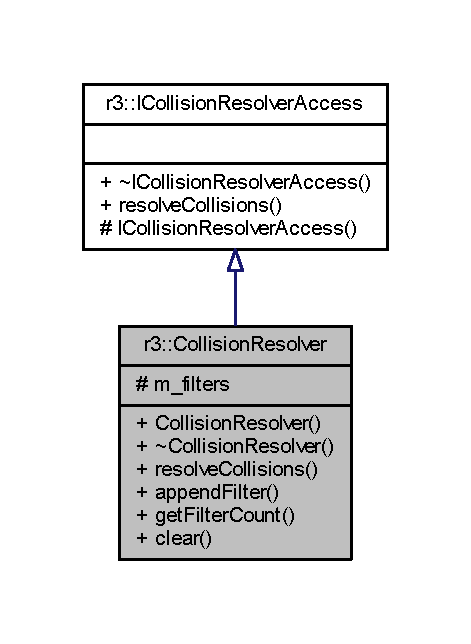
\includegraphics[width=226pt]{classr3_1_1_collision_resolver__inherit__graph}
\end{center}
\end{figure}


Collaboration diagram for r3\+:\+:Collision\+Resolver\+:\nopagebreak
\begin{figure}[H]
\begin{center}
\leavevmode
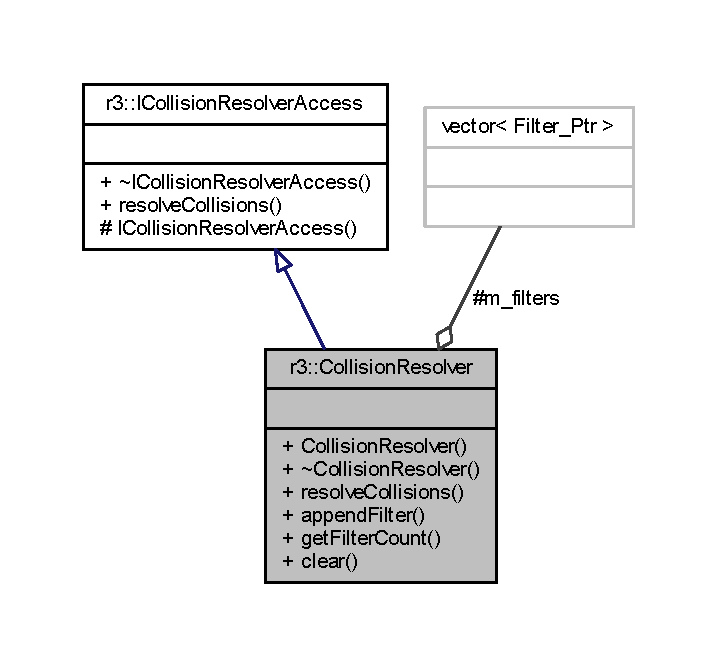
\includegraphics[width=344pt]{classr3_1_1_collision_resolver__coll__graph}
\end{center}
\end{figure}
\subsection*{Public Types}
\begin{DoxyCompactItemize}
\item 
using \mbox{\hyperlink{classr3_1_1_collision_resolver_ad1c9ca40341498c0fe4d483d21c8eb9b}{Filter\+\_\+\+Ptr}} = std\+::unique\+\_\+ptr$<$ \mbox{\hyperlink{classr3_1_1_i_collision_resolution_filter}{I\+Collision\+Resolution\+Filter}} $>$
\end{DoxyCompactItemize}
\subsection*{Public Member Functions}
\begin{DoxyCompactItemize}
\item 
\mbox{\hyperlink{classr3_1_1_collision_resolver_a7b90e276403fa8422879228a189432fb}{Collision\+Resolver}} ()
\item 
virtual \mbox{\hyperlink{classr3_1_1_collision_resolver_ad172d58efecf5ef38f42020f21746f02}{$\sim$\+Collision\+Resolver}} ()
\item 
void \mbox{\hyperlink{classr3_1_1_collision_resolver_a5eeac10ca33299662b0df8a77f6c25f5}{resolve\+Collisions}} (const \mbox{\hyperlink{classr3_1_1_collision_data}{Collision\+Data}} \&collision\+Data) override
\item 
\mbox{\hyperlink{classr3_1_1_i_collision_resolution_filter}{I\+Collision\+Resolution\+Filter}} $\ast$ \mbox{\hyperlink{classr3_1_1_collision_resolver_a9409413937188dbd5332c3440c2a8834}{append\+Filter}} (\mbox{\hyperlink{classr3_1_1_collision_resolver_ad1c9ca40341498c0fe4d483d21c8eb9b}{Filter\+\_\+\+Ptr}} filter)
\begin{DoxyCompactList}\small\item\em Insert a new filter, which will be executed after all already inserted filters. \end{DoxyCompactList}\item 
unsigned int \mbox{\hyperlink{classr3_1_1_collision_resolver_ae56e2125e24982ad368f0d87e9c2a28f}{get\+Filter\+Count}} () const
\item 
void \mbox{\hyperlink{classr3_1_1_collision_resolver_a1f4e3d97afae66c03581807a529678cd}{clear}} ()
\end{DoxyCompactItemize}
\subsection*{Protected Attributes}
\begin{DoxyCompactItemize}
\item 
std\+::vector$<$ \mbox{\hyperlink{classr3_1_1_collision_resolver_ad1c9ca40341498c0fe4d483d21c8eb9b}{Filter\+\_\+\+Ptr}} $>$ \mbox{\hyperlink{classr3_1_1_collision_resolver_abf1234ad45ba7f114b31950c90ccaaff}{m\+\_\+filters}}
\end{DoxyCompactItemize}
\subsection*{Additional Inherited Members}


\subsection{Member Typedef Documentation}
\mbox{\Hypertarget{classr3_1_1_collision_resolver_ad1c9ca40341498c0fe4d483d21c8eb9b}\label{classr3_1_1_collision_resolver_ad1c9ca40341498c0fe4d483d21c8eb9b}} 
\index{r3\+::\+Collision\+Resolver@{r3\+::\+Collision\+Resolver}!Filter\+\_\+\+Ptr@{Filter\+\_\+\+Ptr}}
\index{Filter\+\_\+\+Ptr@{Filter\+\_\+\+Ptr}!r3\+::\+Collision\+Resolver@{r3\+::\+Collision\+Resolver}}
\subsubsection{\texorpdfstring{Filter\+\_\+\+Ptr}{Filter\_Ptr}}
{\footnotesize\ttfamily using \mbox{\hyperlink{classr3_1_1_collision_resolver_ad1c9ca40341498c0fe4d483d21c8eb9b}{r3\+::\+Collision\+Resolver\+::\+Filter\+\_\+\+Ptr}} =  std\+::unique\+\_\+ptr$<$\mbox{\hyperlink{classr3_1_1_i_collision_resolution_filter}{I\+Collision\+Resolution\+Filter}}$>$}



\subsection{Constructor \& Destructor Documentation}
\mbox{\Hypertarget{classr3_1_1_collision_resolver_a7b90e276403fa8422879228a189432fb}\label{classr3_1_1_collision_resolver_a7b90e276403fa8422879228a189432fb}} 
\index{r3\+::\+Collision\+Resolver@{r3\+::\+Collision\+Resolver}!Collision\+Resolver@{Collision\+Resolver}}
\index{Collision\+Resolver@{Collision\+Resolver}!r3\+::\+Collision\+Resolver@{r3\+::\+Collision\+Resolver}}
\subsubsection{\texorpdfstring{Collision\+Resolver()}{CollisionResolver()}}
{\footnotesize\ttfamily r3\+::\+Collision\+Resolver\+::\+Collision\+Resolver (\begin{DoxyParamCaption}{ }\end{DoxyParamCaption})\hspace{0.3cm}{\ttfamily [explicit]}}

\mbox{\Hypertarget{classr3_1_1_collision_resolver_ad172d58efecf5ef38f42020f21746f02}\label{classr3_1_1_collision_resolver_ad172d58efecf5ef38f42020f21746f02}} 
\index{r3\+::\+Collision\+Resolver@{r3\+::\+Collision\+Resolver}!````~Collision\+Resolver@{$\sim$\+Collision\+Resolver}}
\index{````~Collision\+Resolver@{$\sim$\+Collision\+Resolver}!r3\+::\+Collision\+Resolver@{r3\+::\+Collision\+Resolver}}
\subsubsection{\texorpdfstring{$\sim$\+Collision\+Resolver()}{~CollisionResolver()}}
{\footnotesize\ttfamily r3\+::\+Collision\+Resolver\+::$\sim$\+Collision\+Resolver (\begin{DoxyParamCaption}{ }\end{DoxyParamCaption})\hspace{0.3cm}{\ttfamily [virtual]}, {\ttfamily [default]}}



\subsection{Member Function Documentation}
\mbox{\Hypertarget{classr3_1_1_collision_resolver_a9409413937188dbd5332c3440c2a8834}\label{classr3_1_1_collision_resolver_a9409413937188dbd5332c3440c2a8834}} 
\index{r3\+::\+Collision\+Resolver@{r3\+::\+Collision\+Resolver}!append\+Filter@{append\+Filter}}
\index{append\+Filter@{append\+Filter}!r3\+::\+Collision\+Resolver@{r3\+::\+Collision\+Resolver}}
\subsubsection{\texorpdfstring{append\+Filter()}{appendFilter()}}
{\footnotesize\ttfamily \mbox{\hyperlink{classr3_1_1_i_collision_resolution_filter}{I\+Collision\+Resolution\+Filter}} $\ast$ r3\+::\+Collision\+Resolver\+::append\+Filter (\begin{DoxyParamCaption}\item[{\mbox{\hyperlink{classr3_1_1_collision_resolver_ad1c9ca40341498c0fe4d483d21c8eb9b}{Filter\+\_\+\+Ptr}}}]{filter }\end{DoxyParamCaption})}



Insert a new filter, which will be executed after all already inserted filters. 


\begin{DoxyParams}{Parameters}
{\em filter} & The new filter. \\
\hline
\end{DoxyParams}
\begin{DoxyReturn}{Returns}
The new filter. 
\end{DoxyReturn}
\mbox{\Hypertarget{classr3_1_1_collision_resolver_a1f4e3d97afae66c03581807a529678cd}\label{classr3_1_1_collision_resolver_a1f4e3d97afae66c03581807a529678cd}} 
\index{r3\+::\+Collision\+Resolver@{r3\+::\+Collision\+Resolver}!clear@{clear}}
\index{clear@{clear}!r3\+::\+Collision\+Resolver@{r3\+::\+Collision\+Resolver}}
\subsubsection{\texorpdfstring{clear()}{clear()}}
{\footnotesize\ttfamily void r3\+::\+Collision\+Resolver\+::clear (\begin{DoxyParamCaption}{ }\end{DoxyParamCaption})}

Removes all filters from this collision resolver. \mbox{\Hypertarget{classr3_1_1_collision_resolver_ae56e2125e24982ad368f0d87e9c2a28f}\label{classr3_1_1_collision_resolver_ae56e2125e24982ad368f0d87e9c2a28f}} 
\index{r3\+::\+Collision\+Resolver@{r3\+::\+Collision\+Resolver}!get\+Filter\+Count@{get\+Filter\+Count}}
\index{get\+Filter\+Count@{get\+Filter\+Count}!r3\+::\+Collision\+Resolver@{r3\+::\+Collision\+Resolver}}
\subsubsection{\texorpdfstring{get\+Filter\+Count()}{getFilterCount()}}
{\footnotesize\ttfamily unsigned r3\+::\+Collision\+Resolver\+::get\+Filter\+Count (\begin{DoxyParamCaption}{ }\end{DoxyParamCaption}) const}

Get the current number of used filters. \mbox{\Hypertarget{classr3_1_1_collision_resolver_a5eeac10ca33299662b0df8a77f6c25f5}\label{classr3_1_1_collision_resolver_a5eeac10ca33299662b0df8a77f6c25f5}} 
\index{r3\+::\+Collision\+Resolver@{r3\+::\+Collision\+Resolver}!resolve\+Collisions@{resolve\+Collisions}}
\index{resolve\+Collisions@{resolve\+Collisions}!r3\+::\+Collision\+Resolver@{r3\+::\+Collision\+Resolver}}
\subsubsection{\texorpdfstring{resolve\+Collisions()}{resolveCollisions()}}
{\footnotesize\ttfamily void r3\+::\+Collision\+Resolver\+::resolve\+Collisions (\begin{DoxyParamCaption}\item[{const \mbox{\hyperlink{classr3_1_1_collision_data}{Collision\+Data}} \&}]{collision\+Data }\end{DoxyParamCaption})\hspace{0.3cm}{\ttfamily [override]}, {\ttfamily [virtual]}}



Implements \mbox{\hyperlink{classr3_1_1_i_collision_resolver_access_a9f7d7bdd46fa4448b3acc5e79a3c724b}{r3\+::\+I\+Collision\+Resolver\+Access}}.



\subsection{Member Data Documentation}
\mbox{\Hypertarget{classr3_1_1_collision_resolver_abf1234ad45ba7f114b31950c90ccaaff}\label{classr3_1_1_collision_resolver_abf1234ad45ba7f114b31950c90ccaaff}} 
\index{r3\+::\+Collision\+Resolver@{r3\+::\+Collision\+Resolver}!m\+\_\+filters@{m\+\_\+filters}}
\index{m\+\_\+filters@{m\+\_\+filters}!r3\+::\+Collision\+Resolver@{r3\+::\+Collision\+Resolver}}
\subsubsection{\texorpdfstring{m\+\_\+filters}{m\_filters}}
{\footnotesize\ttfamily std\+::vector$<$\mbox{\hyperlink{classr3_1_1_collision_resolver_ad1c9ca40341498c0fe4d483d21c8eb9b}{Filter\+\_\+\+Ptr}}$>$ r3\+::\+Collision\+Resolver\+::m\+\_\+filters\hspace{0.3cm}{\ttfamily [protected]}}



The documentation for this class was generated from the following files\+:\begin{DoxyCompactItemize}
\item 
D\+:/\+Library/\+Documents/\+Job/\+Forschungsmaster/\+Projekte/\+Simulation\+Visualization/\+Rumble3\+D/\+Rumble3\+D/include/\+R3\+D/\+Rigid\+Body\+Engine/\+Collision\+Resolution/\mbox{\hyperlink{_collision_resolver_8h}{Collision\+Resolver.\+h}}\item 
D\+:/\+Library/\+Documents/\+Job/\+Forschungsmaster/\+Projekte/\+Simulation\+Visualization/\+Rumble3\+D/\+Rumble3\+D/src/\+Rigid\+Body\+Engine/\+Collision\+Resolution/\mbox{\hyperlink{_collision_resolver_8cpp}{Collision\+Resolver.\+cpp}}\end{DoxyCompactItemize}

\hypertarget{classr3_1_1_collision_sphere}{}\section{r3\+:\+:Collision\+Sphere Class Reference}
\label{classr3_1_1_collision_sphere}\index{r3\+::\+Collision\+Sphere@{r3\+::\+Collision\+Sphere}}


{\ttfamily \#include $<$Collision\+Sphere.\+h$>$}



Inheritance diagram for r3\+:\+:Collision\+Sphere\+:\nopagebreak
\begin{figure}[H]
\begin{center}
\leavevmode
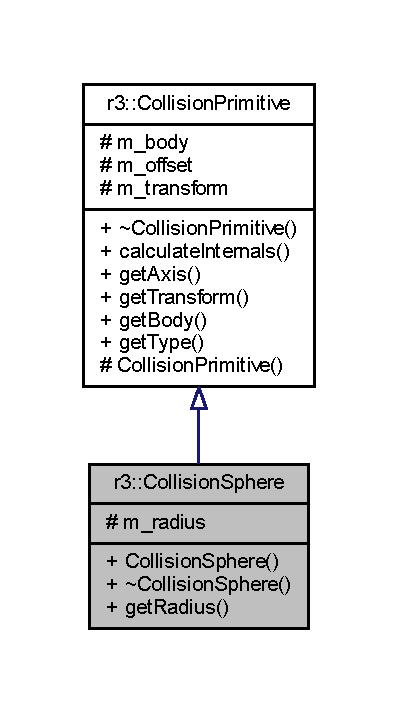
\includegraphics[width=191pt]{classr3_1_1_collision_sphere__inherit__graph}
\end{center}
\end{figure}


Collaboration diagram for r3\+:\+:Collision\+Sphere\+:\nopagebreak
\begin{figure}[H]
\begin{center}
\leavevmode
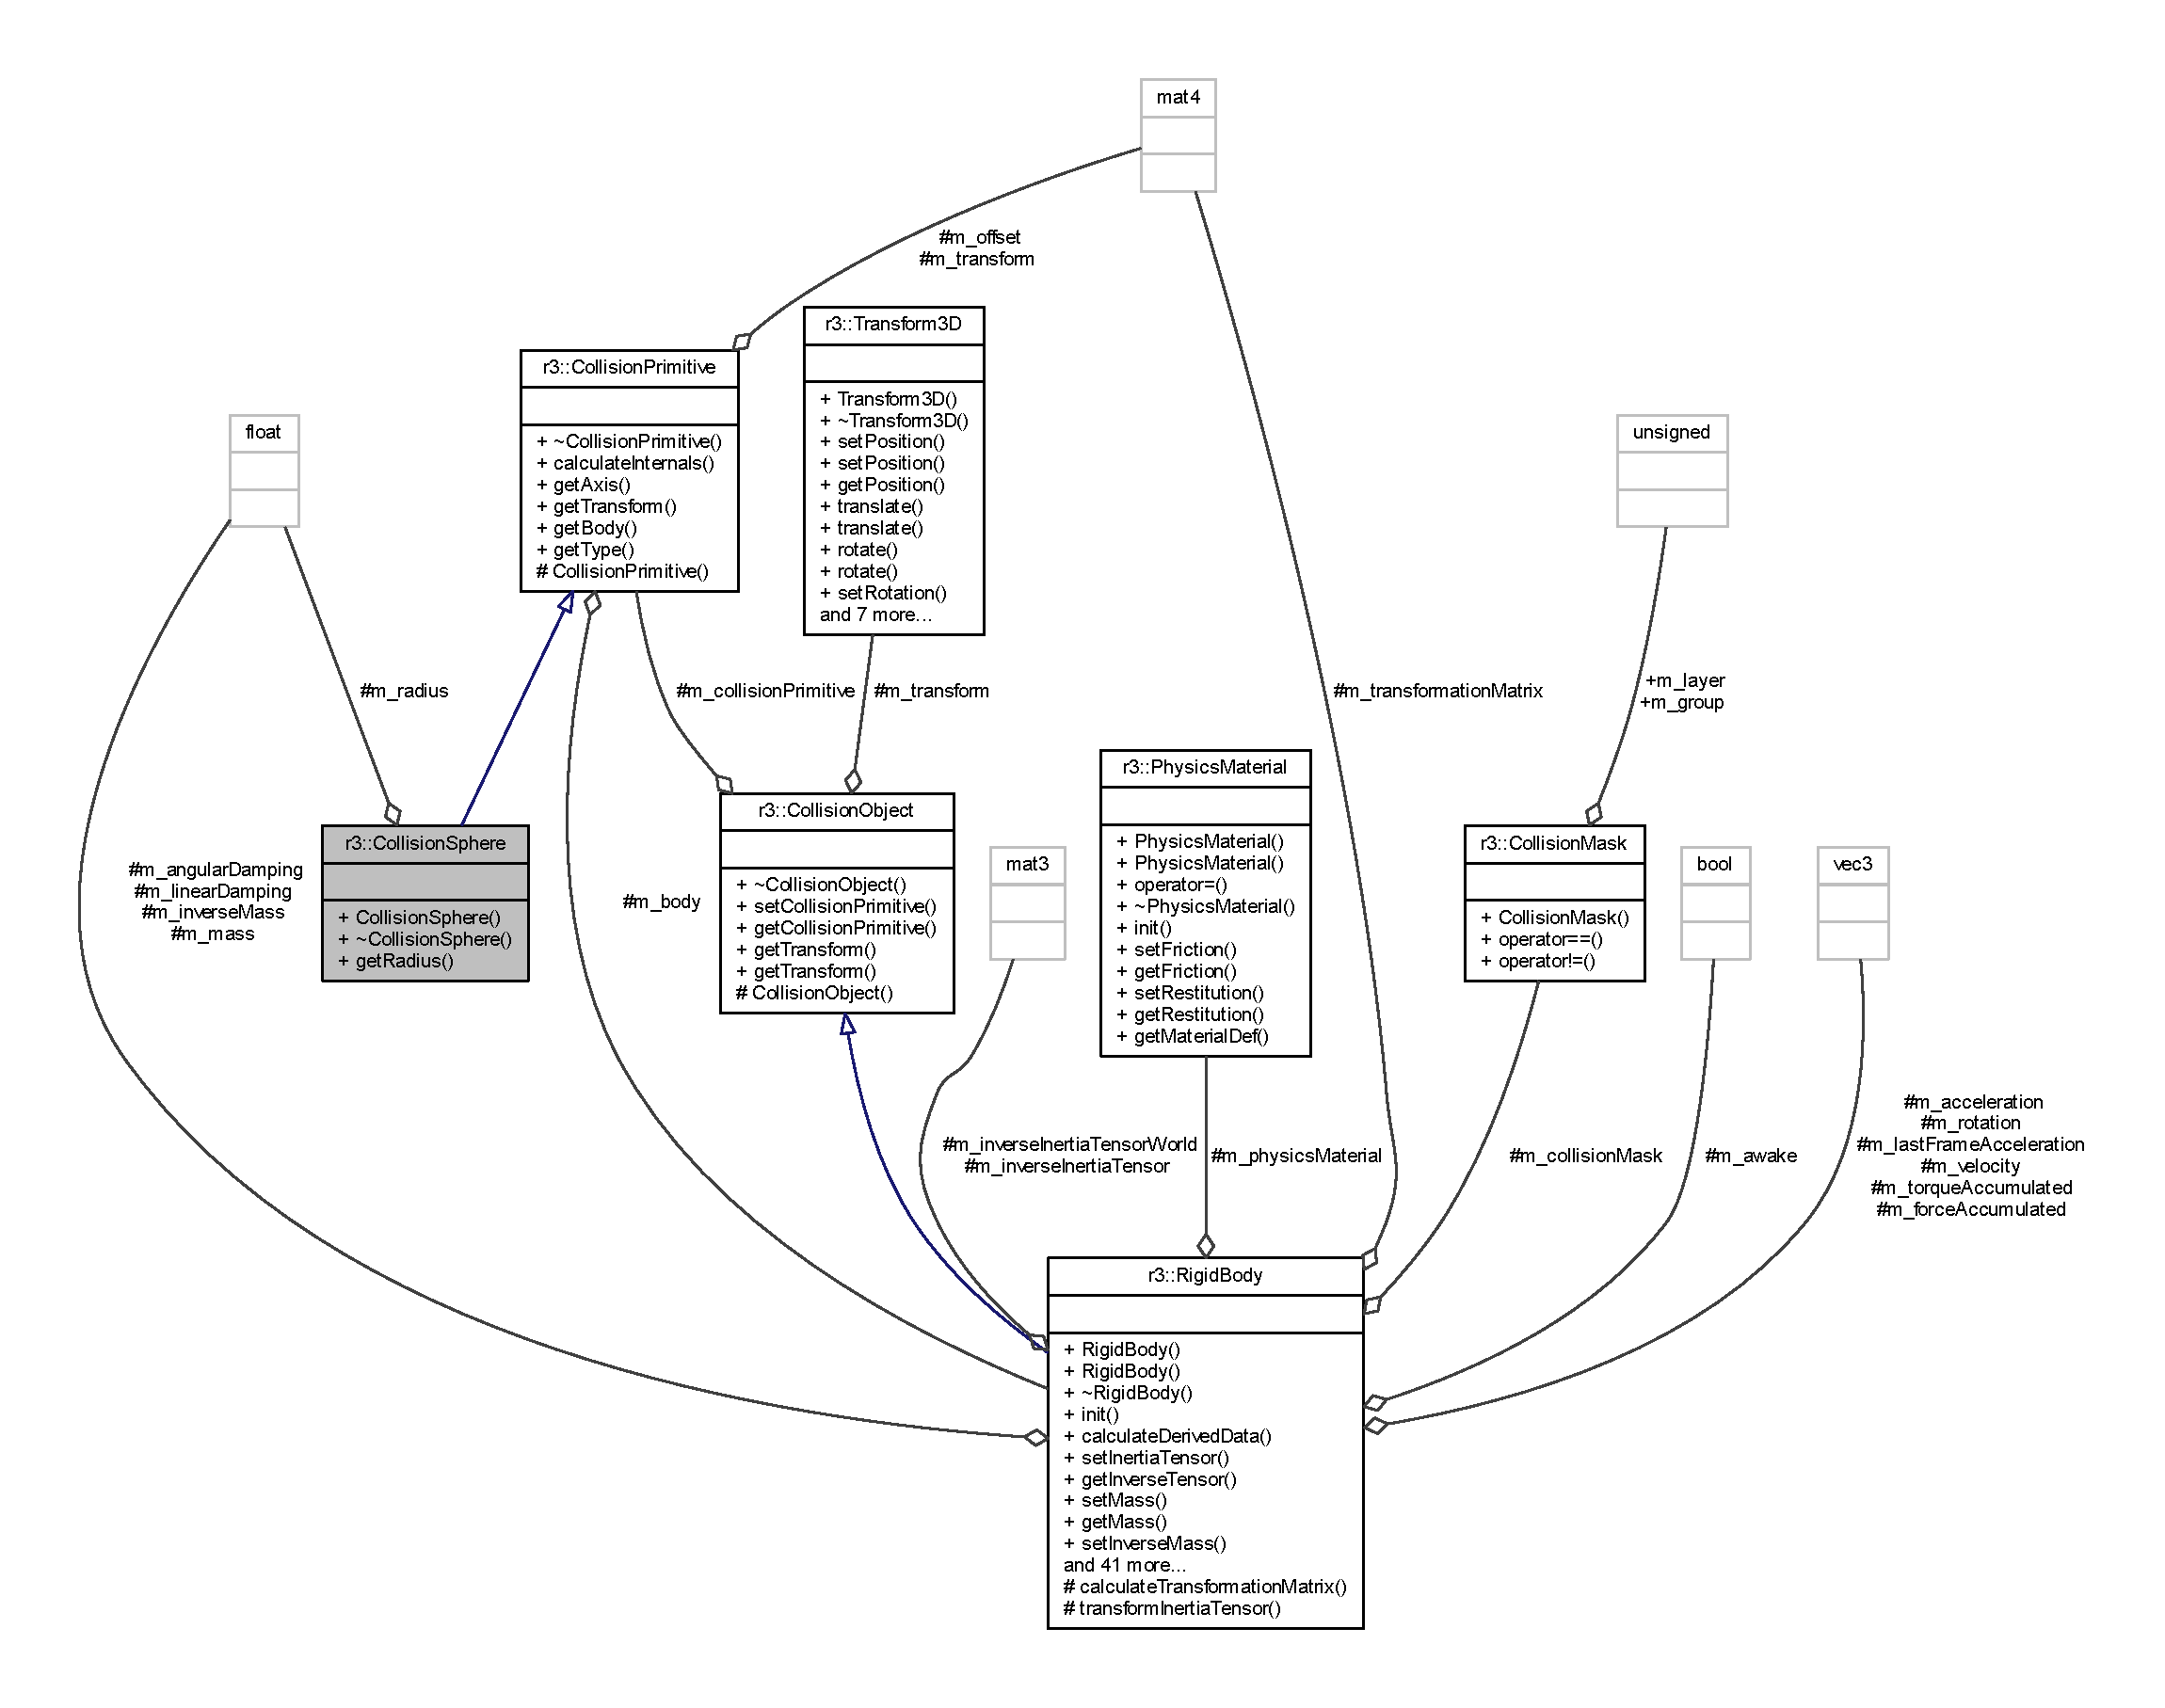
\includegraphics[width=350pt]{classr3_1_1_collision_sphere__coll__graph}
\end{center}
\end{figure}
\subsection*{Public Member Functions}
\begin{DoxyCompactItemize}
\item 
\mbox{\hyperlink{classr3_1_1_collision_sphere_a3b910b66d6b9689da9beba5ec151eba3}{Collision\+Sphere}} (\mbox{\hyperlink{classr3_1_1_rigid_body}{Rigid\+Body}} $\ast$body, \mbox{\hyperlink{namespacer3_ab2016b3e3f743fb735afce242f0dc1eb}{real}} radius, const glm\+::mat4 \&offset=glm\+::mat4(1))
\item 
\mbox{\hyperlink{classr3_1_1_collision_sphere_a3605a7afc888411c5fa52179122a8a77}{$\sim$\+Collision\+Sphere}} ()
\item 
\mbox{\hyperlink{namespacer3_ab2016b3e3f743fb735afce242f0dc1eb}{real}} \mbox{\hyperlink{classr3_1_1_collision_sphere_aa3b7687165b34ab82b3bedb0884cc65b}{get\+Radius}} () const
\end{DoxyCompactItemize}
\subsection*{Protected Attributes}
\begin{DoxyCompactItemize}
\item 
\mbox{\hyperlink{namespacer3_ab2016b3e3f743fb735afce242f0dc1eb}{real}} \mbox{\hyperlink{classr3_1_1_collision_sphere_abc9e3dcae422b4732a288fa19d89d466}{m\+\_\+radius}}
\end{DoxyCompactItemize}
\subsection*{Additional Inherited Members}


\subsection{Constructor \& Destructor Documentation}
\mbox{\Hypertarget{classr3_1_1_collision_sphere_a3b910b66d6b9689da9beba5ec151eba3}\label{classr3_1_1_collision_sphere_a3b910b66d6b9689da9beba5ec151eba3}} 
\index{r3\+::\+Collision\+Sphere@{r3\+::\+Collision\+Sphere}!Collision\+Sphere@{Collision\+Sphere}}
\index{Collision\+Sphere@{Collision\+Sphere}!r3\+::\+Collision\+Sphere@{r3\+::\+Collision\+Sphere}}
\subsubsection{\texorpdfstring{Collision\+Sphere()}{CollisionSphere()}}
{\footnotesize\ttfamily r3\+::\+Collision\+Sphere\+::\+Collision\+Sphere (\begin{DoxyParamCaption}\item[{\mbox{\hyperlink{classr3_1_1_rigid_body}{Rigid\+Body}} $\ast$}]{body,  }\item[{\mbox{\hyperlink{namespacer3_ab2016b3e3f743fb735afce242f0dc1eb}{real}}}]{radius,  }\item[{const glm\+::mat4 \&}]{offset = {\ttfamily glm\+:\+:mat4(1)} }\end{DoxyParamCaption})}

\mbox{\Hypertarget{classr3_1_1_collision_sphere_a3605a7afc888411c5fa52179122a8a77}\label{classr3_1_1_collision_sphere_a3605a7afc888411c5fa52179122a8a77}} 
\index{r3\+::\+Collision\+Sphere@{r3\+::\+Collision\+Sphere}!````~Collision\+Sphere@{$\sim$\+Collision\+Sphere}}
\index{````~Collision\+Sphere@{$\sim$\+Collision\+Sphere}!r3\+::\+Collision\+Sphere@{r3\+::\+Collision\+Sphere}}
\subsubsection{\texorpdfstring{$\sim$\+Collision\+Sphere()}{~CollisionSphere()}}
{\footnotesize\ttfamily r3\+::\+Collision\+Sphere\+::$\sim$\+Collision\+Sphere (\begin{DoxyParamCaption}{ }\end{DoxyParamCaption})\hspace{0.3cm}{\ttfamily [default]}}



\subsection{Member Function Documentation}
\mbox{\Hypertarget{classr3_1_1_collision_sphere_aa3b7687165b34ab82b3bedb0884cc65b}\label{classr3_1_1_collision_sphere_aa3b7687165b34ab82b3bedb0884cc65b}} 
\index{r3\+::\+Collision\+Sphere@{r3\+::\+Collision\+Sphere}!get\+Radius@{get\+Radius}}
\index{get\+Radius@{get\+Radius}!r3\+::\+Collision\+Sphere@{r3\+::\+Collision\+Sphere}}
\subsubsection{\texorpdfstring{get\+Radius()}{getRadius()}}
{\footnotesize\ttfamily \mbox{\hyperlink{namespacer3_ab2016b3e3f743fb735afce242f0dc1eb}{real}} r3\+::\+Collision\+Sphere\+::get\+Radius (\begin{DoxyParamCaption}{ }\end{DoxyParamCaption}) const}



\subsection{Member Data Documentation}
\mbox{\Hypertarget{classr3_1_1_collision_sphere_abc9e3dcae422b4732a288fa19d89d466}\label{classr3_1_1_collision_sphere_abc9e3dcae422b4732a288fa19d89d466}} 
\index{r3\+::\+Collision\+Sphere@{r3\+::\+Collision\+Sphere}!m\+\_\+radius@{m\+\_\+radius}}
\index{m\+\_\+radius@{m\+\_\+radius}!r3\+::\+Collision\+Sphere@{r3\+::\+Collision\+Sphere}}
\subsubsection{\texorpdfstring{m\+\_\+radius}{m\_radius}}
{\footnotesize\ttfamily \mbox{\hyperlink{namespacer3_ab2016b3e3f743fb735afce242f0dc1eb}{real}} r3\+::\+Collision\+Sphere\+::m\+\_\+radius\hspace{0.3cm}{\ttfamily [protected]}}



The documentation for this class was generated from the following files\+:\begin{DoxyCompactItemize}
\item 
D\+:/\+Library/\+Documents/\+Job/\+Forschungsmaster/\+Projekte/\+Simulation\+Visualization/\+Rumble3\+D/\+Rumble3\+D/include/\+R3\+D/\+Rigid\+Body\+Engine/\mbox{\hyperlink{_collision_sphere_8h}{Collision\+Sphere.\+h}}\item 
D\+:/\+Library/\+Documents/\+Job/\+Forschungsmaster/\+Projekte/\+Simulation\+Visualization/\+Rumble3\+D/\+Rumble3\+D/src/\+Rigid\+Body\+Engine/\mbox{\hyperlink{_collision_sphere_8cpp}{Collision\+Sphere.\+cpp}}\end{DoxyCompactItemize}

\hypertarget{classr3_1_1_contact}{}\section{r3\+:\+:Contact Class Reference}
\label{classr3_1_1_contact}\index{r3\+::\+Contact@{r3\+::\+Contact}}


{\ttfamily \#include $<$Contact.\+h$>$}



Collaboration diagram for r3\+:\+:Contact\+:\nopagebreak
\begin{figure}[H]
\begin{center}
\leavevmode
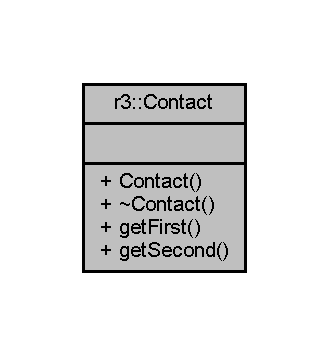
\includegraphics[width=190pt]{classr3_1_1_contact__coll__graph}
\end{center}
\end{figure}
\subsection*{Public Member Functions}
\begin{DoxyCompactItemize}
\item 
\mbox{\hyperlink{classr3_1_1_contact_af2648c9a1e37583ac230a40f4fc6b72d}{Contact}} ()
\item 
\mbox{\hyperlink{classr3_1_1_contact_a011905bfa1cfa3ed459650796b105c6a}{$\sim$\+Contact}} ()
\item 
\mbox{\hyperlink{classr3_1_1_rigid_body}{Rigid\+Body}} $\ast$ \mbox{\hyperlink{classr3_1_1_contact_adf157981ebfd1552521afe7b25e9239c}{get\+First}} () const
\item 
\mbox{\hyperlink{classr3_1_1_rigid_body}{Rigid\+Body}} $\ast$ \mbox{\hyperlink{classr3_1_1_contact_a90af8f5c7cba65a6a84c57b5a6ef6d70}{get\+Second}} () const
\item 
\mbox{\hyperlink{classr3_1_1_rigid_body}{Rigid\+Body}} $\ast$ \mbox{\hyperlink{classr3_1_1_contact_aaa7c4c676fd8f3b07f81cc18257c48d9}{get\+Body}} (int index) const
\item 
void \mbox{\hyperlink{classr3_1_1_contact_aedd044892a1adf0692b7cc9f81b4436a}{set\+Contact\+Point}} (const glm\+::vec3 \&contact\+Point)
\item 
const glm\+::vec3 \& \mbox{\hyperlink{classr3_1_1_contact_a9558ff3dd4e2c5331fc05076e4e503a0}{get\+Contact\+Point}} () const
\item 
void \mbox{\hyperlink{classr3_1_1_contact_af7866e211b169ce6565d3f37af8ef8d7}{set\+Contact\+Normal}} (const glm\+::vec3 \&contact\+Normal)
\item 
glm\+::vec3 \mbox{\hyperlink{classr3_1_1_contact_a2d8f594947a1900fd21e2f707384d9fe}{get\+Contact\+Normal}} () const
\item 
void \mbox{\hyperlink{classr3_1_1_contact_a828feb22ff02fe787739eb5d87cfec38}{set\+Penetration}} (\mbox{\hyperlink{namespacer3_ab2016b3e3f743fb735afce242f0dc1eb}{real}} penetration)
\item 
\mbox{\hyperlink{namespacer3_ab2016b3e3f743fb735afce242f0dc1eb}{real}} \mbox{\hyperlink{classr3_1_1_contact_afe0f0a9a42b4b1f8bd8a61f0b6a4afdd}{get\+Penetration}} () const
\item 
void \mbox{\hyperlink{classr3_1_1_contact_af394998586bc05ec666ffbd06b0f7077}{set\+Body\+Data}} (\mbox{\hyperlink{classr3_1_1_rigid_body}{Rigid\+Body}} $\ast$first, \mbox{\hyperlink{classr3_1_1_rigid_body}{Rigid\+Body}} $\ast$second, \mbox{\hyperlink{namespacer3_ab2016b3e3f743fb735afce242f0dc1eb}{real}} friction, \mbox{\hyperlink{namespacer3_ab2016b3e3f743fb735afce242f0dc1eb}{real}} restitution)
\item 
\mbox{\hyperlink{namespacer3_ab2016b3e3f743fb735afce242f0dc1eb}{real}} \mbox{\hyperlink{classr3_1_1_contact_a1a547c3852733960001cc5fe0fe06790}{get\+Friction}} () const
\item 
\mbox{\hyperlink{namespacer3_ab2016b3e3f743fb735afce242f0dc1eb}{real}} \mbox{\hyperlink{classr3_1_1_contact_a8ec701dcaf82e7fc65bc6c4a2cb6987e}{get\+Restitution}} () const
\item 
glm\+::vec3 \mbox{\hyperlink{classr3_1_1_contact_a733cdbf54fe22bdaaa55a55868ad14ac}{get\+Contact\+Velocity}} () const
\item 
void \mbox{\hyperlink{classr3_1_1_contact_a7ccc2c56a4dcc5b16967f9832fea87ab}{set\+Contact\+Velocity}} (const glm\+::vec3 \&velocity)
\item 
\mbox{\hyperlink{namespacer3_ab2016b3e3f743fb735afce242f0dc1eb}{real}} \mbox{\hyperlink{classr3_1_1_contact_aff234679aa4302b69b8dd101eb969705}{get\+Desired\+Delta\+Velocity}} () const
\item 
void \mbox{\hyperlink{classr3_1_1_contact_a4e00a32cb21ff4fc8ec826f163bcddae}{calculate\+Internals}} (\mbox{\hyperlink{namespacer3_ab2016b3e3f743fb735afce242f0dc1eb}{real}} duration)
\item 
void \mbox{\hyperlink{classr3_1_1_contact_a3f2c146006389bf6273cdd078763b7a3}{calculate\+Desired\+Delta\+Velocity}} (\mbox{\hyperlink{namespacer3_ab2016b3e3f743fb735afce242f0dc1eb}{real}} duration)
\item 
const glm\+::vec3 \& \mbox{\hyperlink{classr3_1_1_contact_ade5794f7055fb30ff52f9193b92c6bf0}{get\+Relative\+Contact\+Position}} (int index) const
\item 
const glm\+::mat3 \& \mbox{\hyperlink{classr3_1_1_contact_a4e9692d870bdba44ff6b627b8c6c6e30}{get\+Contact\+To\+World}} () const
\end{DoxyCompactItemize}


\subsection{Constructor \& Destructor Documentation}
\mbox{\Hypertarget{classr3_1_1_contact_af2648c9a1e37583ac230a40f4fc6b72d}\label{classr3_1_1_contact_af2648c9a1e37583ac230a40f4fc6b72d}} 
\index{r3\+::\+Contact@{r3\+::\+Contact}!Contact@{Contact}}
\index{Contact@{Contact}!r3\+::\+Contact@{r3\+::\+Contact}}
\subsubsection{\texorpdfstring{Contact()}{Contact()}}
{\footnotesize\ttfamily r3\+::\+Contact\+::\+Contact (\begin{DoxyParamCaption}{ }\end{DoxyParamCaption})\hspace{0.3cm}{\ttfamily [explicit]}}

\mbox{\Hypertarget{classr3_1_1_contact_a011905bfa1cfa3ed459650796b105c6a}\label{classr3_1_1_contact_a011905bfa1cfa3ed459650796b105c6a}} 
\index{r3\+::\+Contact@{r3\+::\+Contact}!````~Contact@{$\sim$\+Contact}}
\index{````~Contact@{$\sim$\+Contact}!r3\+::\+Contact@{r3\+::\+Contact}}
\subsubsection{\texorpdfstring{$\sim$\+Contact()}{~Contact()}}
{\footnotesize\ttfamily r3\+::\+Contact\+::$\sim$\+Contact (\begin{DoxyParamCaption}{ }\end{DoxyParamCaption})\hspace{0.3cm}{\ttfamily [default]}}



\subsection{Member Function Documentation}
\mbox{\Hypertarget{classr3_1_1_contact_a3f2c146006389bf6273cdd078763b7a3}\label{classr3_1_1_contact_a3f2c146006389bf6273cdd078763b7a3}} 
\index{r3\+::\+Contact@{r3\+::\+Contact}!calculate\+Desired\+Delta\+Velocity@{calculate\+Desired\+Delta\+Velocity}}
\index{calculate\+Desired\+Delta\+Velocity@{calculate\+Desired\+Delta\+Velocity}!r3\+::\+Contact@{r3\+::\+Contact}}
\subsubsection{\texorpdfstring{calculate\+Desired\+Delta\+Velocity()}{calculateDesiredDeltaVelocity()}}
{\footnotesize\ttfamily void r3\+::\+Contact\+::calculate\+Desired\+Delta\+Velocity (\begin{DoxyParamCaption}\item[{\mbox{\hyperlink{namespacer3_ab2016b3e3f743fb735afce242f0dc1eb}{real}}}]{duration }\end{DoxyParamCaption})}

\mbox{\Hypertarget{classr3_1_1_contact_a4e00a32cb21ff4fc8ec826f163bcddae}\label{classr3_1_1_contact_a4e00a32cb21ff4fc8ec826f163bcddae}} 
\index{r3\+::\+Contact@{r3\+::\+Contact}!calculate\+Internals@{calculate\+Internals}}
\index{calculate\+Internals@{calculate\+Internals}!r3\+::\+Contact@{r3\+::\+Contact}}
\subsubsection{\texorpdfstring{calculate\+Internals()}{calculateInternals()}}
{\footnotesize\ttfamily void r3\+::\+Contact\+::calculate\+Internals (\begin{DoxyParamCaption}\item[{\mbox{\hyperlink{namespacer3_ab2016b3e3f743fb735afce242f0dc1eb}{real}}}]{duration }\end{DoxyParamCaption})}

\mbox{\Hypertarget{classr3_1_1_contact_aaa7c4c676fd8f3b07f81cc18257c48d9}\label{classr3_1_1_contact_aaa7c4c676fd8f3b07f81cc18257c48d9}} 
\index{r3\+::\+Contact@{r3\+::\+Contact}!get\+Body@{get\+Body}}
\index{get\+Body@{get\+Body}!r3\+::\+Contact@{r3\+::\+Contact}}
\subsubsection{\texorpdfstring{get\+Body()}{getBody()}}
{\footnotesize\ttfamily \mbox{\hyperlink{classr3_1_1_rigid_body}{Rigid\+Body}} $\ast$ r3\+::\+Contact\+::get\+Body (\begin{DoxyParamCaption}\item[{int}]{index }\end{DoxyParamCaption}) const}

Get a rigid body by index. \begin{DoxyReturn}{Returns}
The first body if index == 0, the second one if index == 1. 
\end{DoxyReturn}
\mbox{\Hypertarget{classr3_1_1_contact_a2d8f594947a1900fd21e2f707384d9fe}\label{classr3_1_1_contact_a2d8f594947a1900fd21e2f707384d9fe}} 
\index{r3\+::\+Contact@{r3\+::\+Contact}!get\+Contact\+Normal@{get\+Contact\+Normal}}
\index{get\+Contact\+Normal@{get\+Contact\+Normal}!r3\+::\+Contact@{r3\+::\+Contact}}
\subsubsection{\texorpdfstring{get\+Contact\+Normal()}{getContactNormal()}}
{\footnotesize\ttfamily glm\+::vec3 r3\+::\+Contact\+::get\+Contact\+Normal (\begin{DoxyParamCaption}{ }\end{DoxyParamCaption}) const}

Get the direction of the collision at the contact point. \mbox{\Hypertarget{classr3_1_1_contact_a9558ff3dd4e2c5331fc05076e4e503a0}\label{classr3_1_1_contact_a9558ff3dd4e2c5331fc05076e4e503a0}} 
\index{r3\+::\+Contact@{r3\+::\+Contact}!get\+Contact\+Point@{get\+Contact\+Point}}
\index{get\+Contact\+Point@{get\+Contact\+Point}!r3\+::\+Contact@{r3\+::\+Contact}}
\subsubsection{\texorpdfstring{get\+Contact\+Point()}{getContactPoint()}}
{\footnotesize\ttfamily const glm\+::vec3 \& r3\+::\+Contact\+::get\+Contact\+Point (\begin{DoxyParamCaption}{ }\end{DoxyParamCaption}) const}

Get the point, where the collision took place. \mbox{\Hypertarget{classr3_1_1_contact_a4e9692d870bdba44ff6b627b8c6c6e30}\label{classr3_1_1_contact_a4e9692d870bdba44ff6b627b8c6c6e30}} 
\index{r3\+::\+Contact@{r3\+::\+Contact}!get\+Contact\+To\+World@{get\+Contact\+To\+World}}
\index{get\+Contact\+To\+World@{get\+Contact\+To\+World}!r3\+::\+Contact@{r3\+::\+Contact}}
\subsubsection{\texorpdfstring{get\+Contact\+To\+World()}{getContactToWorld()}}
{\footnotesize\ttfamily const glm\+::mat3 \& r3\+::\+Contact\+::get\+Contact\+To\+World (\begin{DoxyParamCaption}{ }\end{DoxyParamCaption}) const}

\mbox{\Hypertarget{classr3_1_1_contact_a733cdbf54fe22bdaaa55a55868ad14ac}\label{classr3_1_1_contact_a733cdbf54fe22bdaaa55a55868ad14ac}} 
\index{r3\+::\+Contact@{r3\+::\+Contact}!get\+Contact\+Velocity@{get\+Contact\+Velocity}}
\index{get\+Contact\+Velocity@{get\+Contact\+Velocity}!r3\+::\+Contact@{r3\+::\+Contact}}
\subsubsection{\texorpdfstring{get\+Contact\+Velocity()}{getContactVelocity()}}
{\footnotesize\ttfamily glm\+::vec3 r3\+::\+Contact\+::get\+Contact\+Velocity (\begin{DoxyParamCaption}{ }\end{DoxyParamCaption}) const}

\mbox{\Hypertarget{classr3_1_1_contact_aff234679aa4302b69b8dd101eb969705}\label{classr3_1_1_contact_aff234679aa4302b69b8dd101eb969705}} 
\index{r3\+::\+Contact@{r3\+::\+Contact}!get\+Desired\+Delta\+Velocity@{get\+Desired\+Delta\+Velocity}}
\index{get\+Desired\+Delta\+Velocity@{get\+Desired\+Delta\+Velocity}!r3\+::\+Contact@{r3\+::\+Contact}}
\subsubsection{\texorpdfstring{get\+Desired\+Delta\+Velocity()}{getDesiredDeltaVelocity()}}
{\footnotesize\ttfamily \mbox{\hyperlink{namespacer3_ab2016b3e3f743fb735afce242f0dc1eb}{real}} r3\+::\+Contact\+::get\+Desired\+Delta\+Velocity (\begin{DoxyParamCaption}{ }\end{DoxyParamCaption}) const}

\mbox{\Hypertarget{classr3_1_1_contact_adf157981ebfd1552521afe7b25e9239c}\label{classr3_1_1_contact_adf157981ebfd1552521afe7b25e9239c}} 
\index{r3\+::\+Contact@{r3\+::\+Contact}!get\+First@{get\+First}}
\index{get\+First@{get\+First}!r3\+::\+Contact@{r3\+::\+Contact}}
\subsubsection{\texorpdfstring{get\+First()}{getFirst()}}
{\footnotesize\ttfamily \mbox{\hyperlink{classr3_1_1_rigid_body}{Rigid\+Body}} $\ast$ r3\+::\+Contact\+::get\+First (\begin{DoxyParamCaption}{ }\end{DoxyParamCaption}) const}

Get the first colliding rigid body. \mbox{\Hypertarget{classr3_1_1_contact_a1a547c3852733960001cc5fe0fe06790}\label{classr3_1_1_contact_a1a547c3852733960001cc5fe0fe06790}} 
\index{r3\+::\+Contact@{r3\+::\+Contact}!get\+Friction@{get\+Friction}}
\index{get\+Friction@{get\+Friction}!r3\+::\+Contact@{r3\+::\+Contact}}
\subsubsection{\texorpdfstring{get\+Friction()}{getFriction()}}
{\footnotesize\ttfamily \mbox{\hyperlink{namespacer3_ab2016b3e3f743fb735afce242f0dc1eb}{real}} r3\+::\+Contact\+::get\+Friction (\begin{DoxyParamCaption}{ }\end{DoxyParamCaption}) const}

Get the friction constant. \mbox{\Hypertarget{classr3_1_1_contact_afe0f0a9a42b4b1f8bd8a61f0b6a4afdd}\label{classr3_1_1_contact_afe0f0a9a42b4b1f8bd8a61f0b6a4afdd}} 
\index{r3\+::\+Contact@{r3\+::\+Contact}!get\+Penetration@{get\+Penetration}}
\index{get\+Penetration@{get\+Penetration}!r3\+::\+Contact@{r3\+::\+Contact}}
\subsubsection{\texorpdfstring{get\+Penetration()}{getPenetration()}}
{\footnotesize\ttfamily \mbox{\hyperlink{namespacer3_ab2016b3e3f743fb735afce242f0dc1eb}{real}} r3\+::\+Contact\+::get\+Penetration (\begin{DoxyParamCaption}{ }\end{DoxyParamCaption}) const}

Get the amount of interpenetration. \mbox{\Hypertarget{classr3_1_1_contact_ade5794f7055fb30ff52f9193b92c6bf0}\label{classr3_1_1_contact_ade5794f7055fb30ff52f9193b92c6bf0}} 
\index{r3\+::\+Contact@{r3\+::\+Contact}!get\+Relative\+Contact\+Position@{get\+Relative\+Contact\+Position}}
\index{get\+Relative\+Contact\+Position@{get\+Relative\+Contact\+Position}!r3\+::\+Contact@{r3\+::\+Contact}}
\subsubsection{\texorpdfstring{get\+Relative\+Contact\+Position()}{getRelativeContactPosition()}}
{\footnotesize\ttfamily const glm\+::vec3 \& r3\+::\+Contact\+::get\+Relative\+Contact\+Position (\begin{DoxyParamCaption}\item[{int}]{index }\end{DoxyParamCaption}) const}

\mbox{\Hypertarget{classr3_1_1_contact_a8ec701dcaf82e7fc65bc6c4a2cb6987e}\label{classr3_1_1_contact_a8ec701dcaf82e7fc65bc6c4a2cb6987e}} 
\index{r3\+::\+Contact@{r3\+::\+Contact}!get\+Restitution@{get\+Restitution}}
\index{get\+Restitution@{get\+Restitution}!r3\+::\+Contact@{r3\+::\+Contact}}
\subsubsection{\texorpdfstring{get\+Restitution()}{getRestitution()}}
{\footnotesize\ttfamily \mbox{\hyperlink{namespacer3_ab2016b3e3f743fb735afce242f0dc1eb}{real}} r3\+::\+Contact\+::get\+Restitution (\begin{DoxyParamCaption}{ }\end{DoxyParamCaption}) const}

Get the restitution constant. \mbox{\Hypertarget{classr3_1_1_contact_a90af8f5c7cba65a6a84c57b5a6ef6d70}\label{classr3_1_1_contact_a90af8f5c7cba65a6a84c57b5a6ef6d70}} 
\index{r3\+::\+Contact@{r3\+::\+Contact}!get\+Second@{get\+Second}}
\index{get\+Second@{get\+Second}!r3\+::\+Contact@{r3\+::\+Contact}}
\subsubsection{\texorpdfstring{get\+Second()}{getSecond()}}
{\footnotesize\ttfamily \mbox{\hyperlink{classr3_1_1_rigid_body}{Rigid\+Body}} $\ast$ r3\+::\+Contact\+::get\+Second (\begin{DoxyParamCaption}{ }\end{DoxyParamCaption}) const}

Get the second colliding rigid body. \mbox{\Hypertarget{classr3_1_1_contact_af394998586bc05ec666ffbd06b0f7077}\label{classr3_1_1_contact_af394998586bc05ec666ffbd06b0f7077}} 
\index{r3\+::\+Contact@{r3\+::\+Contact}!set\+Body\+Data@{set\+Body\+Data}}
\index{set\+Body\+Data@{set\+Body\+Data}!r3\+::\+Contact@{r3\+::\+Contact}}
\subsubsection{\texorpdfstring{set\+Body\+Data()}{setBodyData()}}
{\footnotesize\ttfamily void r3\+::\+Contact\+::set\+Body\+Data (\begin{DoxyParamCaption}\item[{\mbox{\hyperlink{classr3_1_1_rigid_body}{Rigid\+Body}} $\ast$}]{first,  }\item[{\mbox{\hyperlink{classr3_1_1_rigid_body}{Rigid\+Body}} $\ast$}]{second,  }\item[{\mbox{\hyperlink{namespacer3_ab2016b3e3f743fb735afce242f0dc1eb}{real}}}]{friction,  }\item[{\mbox{\hyperlink{namespacer3_ab2016b3e3f743fb735afce242f0dc1eb}{real}}}]{restitution }\end{DoxyParamCaption})}

Set involved rigid bodies, friction and restitution coefficients. \mbox{\Hypertarget{classr3_1_1_contact_af7866e211b169ce6565d3f37af8ef8d7}\label{classr3_1_1_contact_af7866e211b169ce6565d3f37af8ef8d7}} 
\index{r3\+::\+Contact@{r3\+::\+Contact}!set\+Contact\+Normal@{set\+Contact\+Normal}}
\index{set\+Contact\+Normal@{set\+Contact\+Normal}!r3\+::\+Contact@{r3\+::\+Contact}}
\subsubsection{\texorpdfstring{set\+Contact\+Normal()}{setContactNormal()}}
{\footnotesize\ttfamily void r3\+::\+Contact\+::set\+Contact\+Normal (\begin{DoxyParamCaption}\item[{const glm\+::vec3 \&}]{contact\+Normal }\end{DoxyParamCaption})}

Set the direction of the collision at the contact point. \mbox{\Hypertarget{classr3_1_1_contact_aedd044892a1adf0692b7cc9f81b4436a}\label{classr3_1_1_contact_aedd044892a1adf0692b7cc9f81b4436a}} 
\index{r3\+::\+Contact@{r3\+::\+Contact}!set\+Contact\+Point@{set\+Contact\+Point}}
\index{set\+Contact\+Point@{set\+Contact\+Point}!r3\+::\+Contact@{r3\+::\+Contact}}
\subsubsection{\texorpdfstring{set\+Contact\+Point()}{setContactPoint()}}
{\footnotesize\ttfamily void r3\+::\+Contact\+::set\+Contact\+Point (\begin{DoxyParamCaption}\item[{const glm\+::vec3 \&}]{contact\+Point }\end{DoxyParamCaption})}

Set the point, where the collision took place. \mbox{\Hypertarget{classr3_1_1_contact_a7ccc2c56a4dcc5b16967f9832fea87ab}\label{classr3_1_1_contact_a7ccc2c56a4dcc5b16967f9832fea87ab}} 
\index{r3\+::\+Contact@{r3\+::\+Contact}!set\+Contact\+Velocity@{set\+Contact\+Velocity}}
\index{set\+Contact\+Velocity@{set\+Contact\+Velocity}!r3\+::\+Contact@{r3\+::\+Contact}}
\subsubsection{\texorpdfstring{set\+Contact\+Velocity()}{setContactVelocity()}}
{\footnotesize\ttfamily void r3\+::\+Contact\+::set\+Contact\+Velocity (\begin{DoxyParamCaption}\item[{const glm\+::vec3 \&}]{velocity }\end{DoxyParamCaption})}

\mbox{\Hypertarget{classr3_1_1_contact_a828feb22ff02fe787739eb5d87cfec38}\label{classr3_1_1_contact_a828feb22ff02fe787739eb5d87cfec38}} 
\index{r3\+::\+Contact@{r3\+::\+Contact}!set\+Penetration@{set\+Penetration}}
\index{set\+Penetration@{set\+Penetration}!r3\+::\+Contact@{r3\+::\+Contact}}
\subsubsection{\texorpdfstring{set\+Penetration()}{setPenetration()}}
{\footnotesize\ttfamily void r3\+::\+Contact\+::set\+Penetration (\begin{DoxyParamCaption}\item[{\mbox{\hyperlink{namespacer3_ab2016b3e3f743fb735afce242f0dc1eb}{real}}}]{penetration }\end{DoxyParamCaption})}

Set the amount of interpenetration along the contact normal. 

The documentation for this class was generated from the following files\+:\begin{DoxyCompactItemize}
\item 
D\+:/\+Job/\+Forschungsmaster/\+Projekte/\+Simulation\+Visualization/\+Rumble3\+D/\+Rumble3\+D/include/\+R3\+D/\+Rigid\+Body\+Engine/\+Collision\+Detection/\mbox{\hyperlink{_contact_8h}{Contact.\+h}}\item 
D\+:/\+Job/\+Forschungsmaster/\+Projekte/\+Simulation\+Visualization/\+Rumble3\+D/\+Rumble3\+D/src/\+Rigid\+Body\+Engine/\+Collision\+Detection/\mbox{\hyperlink{_contact_8cpp}{Contact.\+cpp}}\end{DoxyCompactItemize}

\hypertarget{classr3_1_1_contact_generator}{}\section{r3\+:\+:Contact\+Generator Class Reference}
\label{classr3_1_1_contact_generator}\index{r3\+::\+Contact\+Generator@{r3\+::\+Contact\+Generator}}


{\ttfamily \#include $<$Contact\+Generator.\+h$>$}



Collaboration diagram for r3\+:\+:Contact\+Generator\+:\nopagebreak
\begin{figure}[H]
\begin{center}
\leavevmode
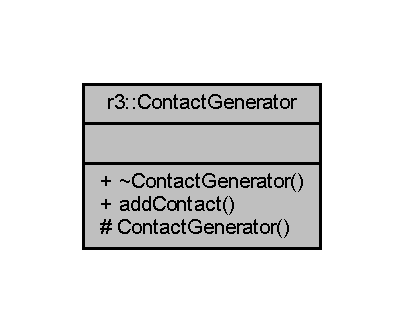
\includegraphics[width=194pt]{classr3_1_1_contact_generator__coll__graph}
\end{center}
\end{figure}
\subsection*{Public Member Functions}
\begin{DoxyCompactItemize}
\item 
virtual \mbox{\hyperlink{classr3_1_1_contact_generator_a5b44b4e2b114259c30eae2d5d0ca4202}{$\sim$\+Contact\+Generator}} ()
\item 
virtual unsigned \mbox{\hyperlink{classr3_1_1_contact_generator_ad72e6b61035d682f3d424cbd0c6d73c3}{add\+Contact}} (\mbox{\hyperlink{classr3_1_1_contact_old}{Contact\+Old}} $\ast$contact, unsigned limit) const
\end{DoxyCompactItemize}
\subsection*{Protected Member Functions}
\begin{DoxyCompactItemize}
\item 
\mbox{\hyperlink{classr3_1_1_contact_generator_ae71d8c8d7e9e57ba10de178fe12b4084}{Contact\+Generator}} ()
\end{DoxyCompactItemize}


\subsection{Constructor \& Destructor Documentation}
\mbox{\Hypertarget{classr3_1_1_contact_generator_a5b44b4e2b114259c30eae2d5d0ca4202}\label{classr3_1_1_contact_generator_a5b44b4e2b114259c30eae2d5d0ca4202}} 
\index{r3\+::\+Contact\+Generator@{r3\+::\+Contact\+Generator}!````~Contact\+Generator@{$\sim$\+Contact\+Generator}}
\index{````~Contact\+Generator@{$\sim$\+Contact\+Generator}!r3\+::\+Contact\+Generator@{r3\+::\+Contact\+Generator}}
\subsubsection{\texorpdfstring{$\sim$\+Contact\+Generator()}{~ContactGenerator()}}
{\footnotesize\ttfamily r3\+::\+Contact\+Generator\+::$\sim$\+Contact\+Generator (\begin{DoxyParamCaption}{ }\end{DoxyParamCaption})\hspace{0.3cm}{\ttfamily [virtual]}, {\ttfamily [default]}}

\mbox{\Hypertarget{classr3_1_1_contact_generator_ae71d8c8d7e9e57ba10de178fe12b4084}\label{classr3_1_1_contact_generator_ae71d8c8d7e9e57ba10de178fe12b4084}} 
\index{r3\+::\+Contact\+Generator@{r3\+::\+Contact\+Generator}!Contact\+Generator@{Contact\+Generator}}
\index{Contact\+Generator@{Contact\+Generator}!r3\+::\+Contact\+Generator@{r3\+::\+Contact\+Generator}}
\subsubsection{\texorpdfstring{Contact\+Generator()}{ContactGenerator()}}
{\footnotesize\ttfamily r3\+::\+Contact\+Generator\+::\+Contact\+Generator (\begin{DoxyParamCaption}{ }\end{DoxyParamCaption})\hspace{0.3cm}{\ttfamily [explicit]}, {\ttfamily [protected]}, {\ttfamily [default]}}



\subsection{Member Function Documentation}
\mbox{\Hypertarget{classr3_1_1_contact_generator_ad72e6b61035d682f3d424cbd0c6d73c3}\label{classr3_1_1_contact_generator_ad72e6b61035d682f3d424cbd0c6d73c3}} 
\index{r3\+::\+Contact\+Generator@{r3\+::\+Contact\+Generator}!add\+Contact@{add\+Contact}}
\index{add\+Contact@{add\+Contact}!r3\+::\+Contact\+Generator@{r3\+::\+Contact\+Generator}}
\subsubsection{\texorpdfstring{add\+Contact()}{addContact()}}
{\footnotesize\ttfamily virtual unsigned r3\+::\+Contact\+Generator\+::add\+Contact (\begin{DoxyParamCaption}\item[{\mbox{\hyperlink{classr3_1_1_contact_old}{Contact\+Old}} $\ast$}]{contact,  }\item[{unsigned}]{limit }\end{DoxyParamCaption}) const\hspace{0.3cm}{\ttfamily [virtual]}}



The documentation for this class was generated from the following files\+:\begin{DoxyCompactItemize}
\item 
D\+:/\+Library/\+Documents/\+Job/\+Forschungsmaster/\+Projekte/\+Simulation\+Visualization/\+Rumble3\+D/\+Rumble3\+D/include/\+R3\+D/\+Rigid\+Body\+Engine/\mbox{\hyperlink{_contact_generator_8h}{Contact\+Generator.\+h}}\item 
D\+:/\+Library/\+Documents/\+Job/\+Forschungsmaster/\+Projekte/\+Simulation\+Visualization/\+Rumble3\+D/\+Rumble3\+D/src/\+Rigid\+Body\+Engine/\mbox{\hyperlink{_contact_generator_8cpp}{Contact\+Generator.\+cpp}}\end{DoxyCompactItemize}

\hypertarget{classr3_1_1_contact_old}{}\section{r3\+:\+:Contact\+Old Class Reference}
\label{classr3_1_1_contact_old}\index{r3\+::\+Contact\+Old@{r3\+::\+Contact\+Old}}


{\ttfamily \#include $<$Contact\+Old.\+h$>$}



Collaboration diagram for r3\+:\+:Contact\+Old\+:\nopagebreak
\begin{figure}[H]
\begin{center}
\leavevmode
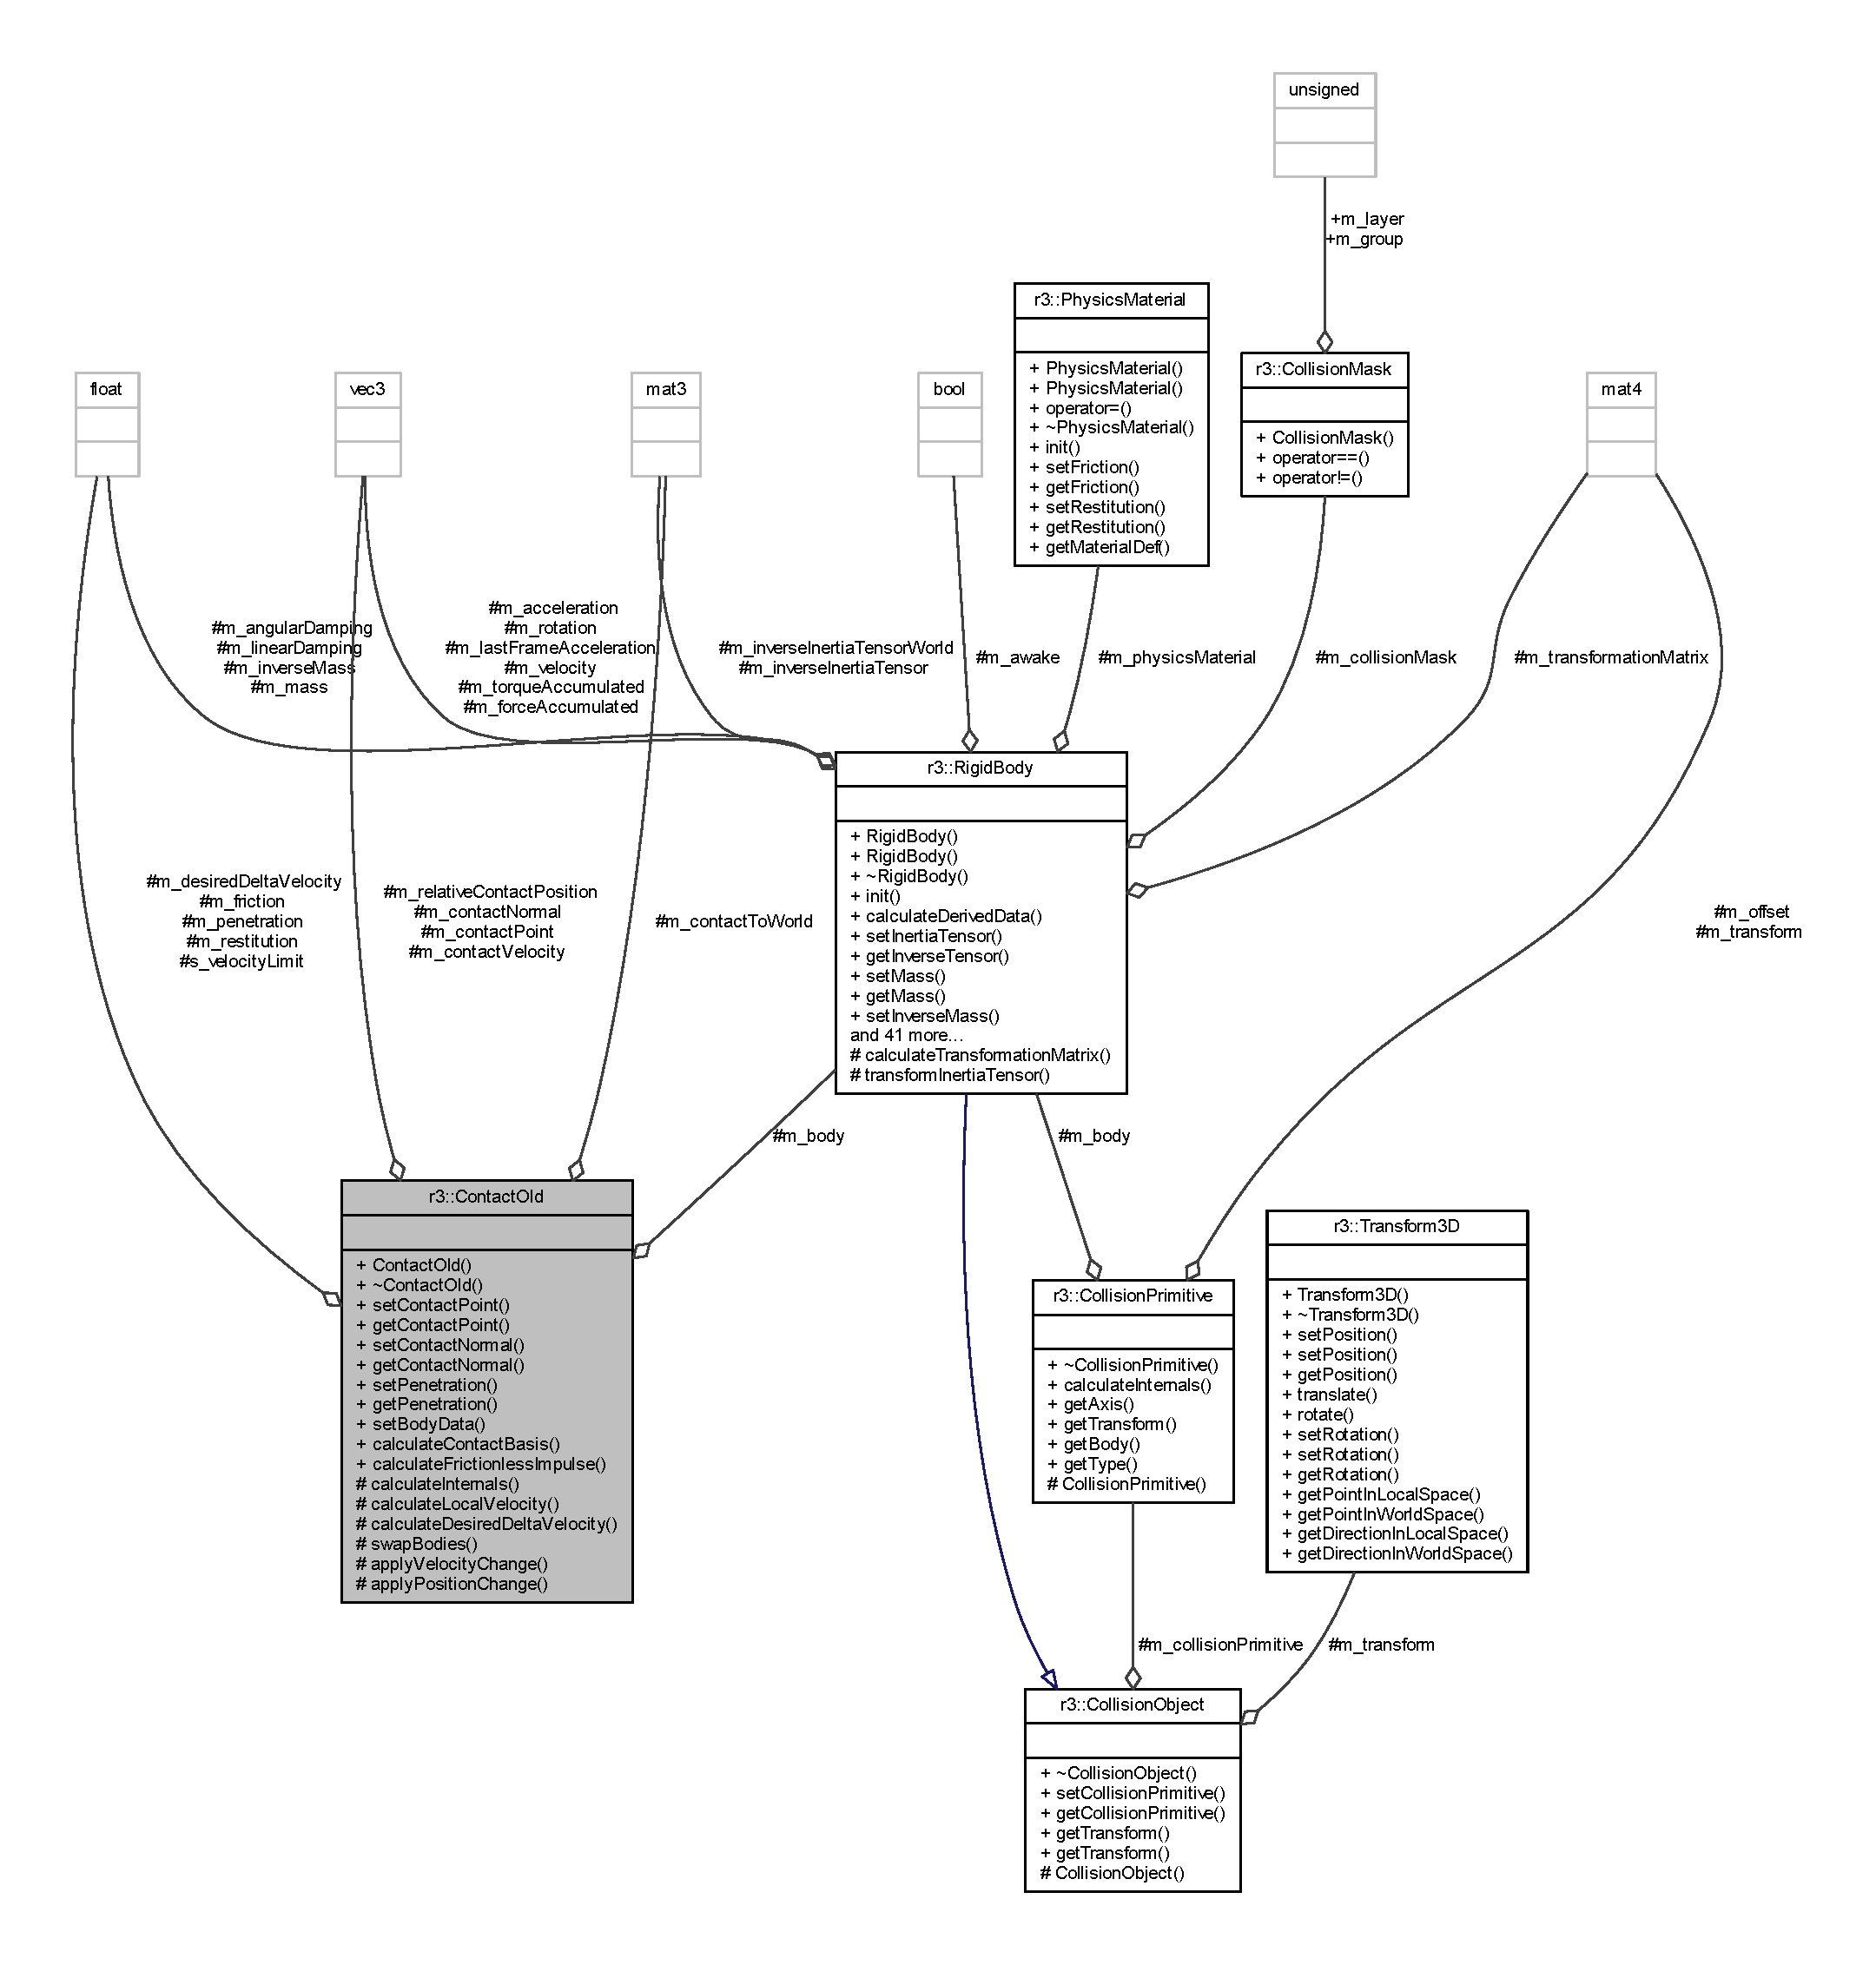
\includegraphics[width=350pt]{classr3_1_1_contact_old__coll__graph}
\end{center}
\end{figure}
\subsection*{Public Member Functions}
\begin{DoxyCompactItemize}
\item 
\mbox{\hyperlink{classr3_1_1_contact_old_aceb62b2ac59cc25dac229907570a1258}{Contact\+Old}} ()
\item 
\mbox{\hyperlink{classr3_1_1_contact_old_acd1e3d9a18b6b95e1937ff6a5f3d32e4}{$\sim$\+Contact\+Old}} ()
\item 
void \mbox{\hyperlink{classr3_1_1_contact_old_a389520942ce68e49b6a5350a8fcd30a1}{set\+Contact\+Point}} (const glm\+::vec3 \&contact\+Point)
\item 
glm\+::vec3 \mbox{\hyperlink{classr3_1_1_contact_old_a1af4ec25d791c0f14e41747e231fd6ab}{get\+Contact\+Point}} () const
\item 
void \mbox{\hyperlink{classr3_1_1_contact_old_a9556b3cbd099762435cf0f594a43b6c9}{set\+Contact\+Normal}} (const glm\+::vec3 \&contact\+Normal)
\item 
glm\+::vec3 \mbox{\hyperlink{classr3_1_1_contact_old_affb54494fd3c883cc6acf4f1b9fbc639}{get\+Contact\+Normal}} () const
\item 
void \mbox{\hyperlink{classr3_1_1_contact_old_a66490bf2da7cee1795614e96d5db405f}{set\+Penetration}} (\mbox{\hyperlink{namespacer3_ab2016b3e3f743fb735afce242f0dc1eb}{real}} penetration)
\item 
\mbox{\hyperlink{namespacer3_ab2016b3e3f743fb735afce242f0dc1eb}{real}} \mbox{\hyperlink{classr3_1_1_contact_old_a2ef64745c0b7d6370f886ed002697044}{get\+Penetration}} () const
\item 
void \mbox{\hyperlink{classr3_1_1_contact_old_a7ec291b8cb62e1786f981831ce336f43}{set\+Body\+Data}} (\mbox{\hyperlink{classr3_1_1_rigid_body}{Rigid\+Body}} $\ast$one, \mbox{\hyperlink{classr3_1_1_rigid_body}{Rigid\+Body}} $\ast$two, \mbox{\hyperlink{namespacer3_ab2016b3e3f743fb735afce242f0dc1eb}{real}} friction, \mbox{\hyperlink{namespacer3_ab2016b3e3f743fb735afce242f0dc1eb}{real}} restitution)
\item 
void \mbox{\hyperlink{classr3_1_1_contact_old_a48506cebe73d8bac8fadf2cc3d029be8}{calculate\+Contact\+Basis}} ()
\item 
glm\+::vec3 \mbox{\hyperlink{classr3_1_1_contact_old_aeefaeffa952d193238cc47afeaa098e2}{calculate\+Frictionless\+Impulse}} (glm\+::mat3 $\ast$inverse\+Inertia\+Tensor) const
\end{DoxyCompactItemize}
\subsection*{Protected Member Functions}
\begin{DoxyCompactItemize}
\item 
void \mbox{\hyperlink{classr3_1_1_contact_old_a1a14824b3762a34187d68a920e0a4419}{calculate\+Internals}} (\mbox{\hyperlink{namespacer3_ab2016b3e3f743fb735afce242f0dc1eb}{real}} duration)
\item 
glm\+::vec3 \mbox{\hyperlink{classr3_1_1_contact_old_a887dcd47a9488b70d07d2cfd319a44a9}{calculate\+Local\+Velocity}} (unsigned body\+Index, \mbox{\hyperlink{namespacer3_ab2016b3e3f743fb735afce242f0dc1eb}{real}} duration)
\item 
void \mbox{\hyperlink{classr3_1_1_contact_old_a425c2ea555131d0c2c5a74c8aa375e82}{calculate\+Desired\+Delta\+Velocity}} (\mbox{\hyperlink{namespacer3_ab2016b3e3f743fb735afce242f0dc1eb}{real}} duration)
\item 
void \mbox{\hyperlink{classr3_1_1_contact_old_a9dedf16b72b57cfa3f5a007bd02ac6ab}{swap\+Bodies}} ()
\item 
void \mbox{\hyperlink{classr3_1_1_contact_old_a81284d6f3922ccdccff5bfbbf4d9f7de}{apply\+Velocity\+Change}} (glm\+::vec3 velocity\+Change\mbox{[}2\mbox{]}, glm\+::vec3 rotation\+Change\mbox{[}2\mbox{]}) const
\item 
void \mbox{\hyperlink{classr3_1_1_contact_old_a2f4e9562823687d3f5c3994f21cd3020}{apply\+Position\+Change}} (glm\+::vec3 linear\+Change\mbox{[}2\mbox{]}, glm\+::vec3 angular\+Change\mbox{[}2\mbox{]}, \mbox{\hyperlink{namespacer3_ab2016b3e3f743fb735afce242f0dc1eb}{real}} penetration) const
\end{DoxyCompactItemize}
\subsection*{Protected Attributes}
\begin{DoxyCompactItemize}
\item 
\mbox{\hyperlink{classr3_1_1_rigid_body}{Rigid\+Body}} $\ast$ \mbox{\hyperlink{classr3_1_1_contact_old_aa429e9cfd0ccb3216cf85b53fb9c98a2}{m\+\_\+body}} \mbox{[}2\mbox{]} \{\}
\begin{DoxyCompactList}\small\item\em The two rigid bodies, which are colliding. \end{DoxyCompactList}\item 
\mbox{\hyperlink{namespacer3_ab2016b3e3f743fb735afce242f0dc1eb}{real}} \mbox{\hyperlink{classr3_1_1_contact_old_a699b5339e2ea93550be5b977f8588a8d}{m\+\_\+friction}} \{\}
\item 
\mbox{\hyperlink{namespacer3_ab2016b3e3f743fb735afce242f0dc1eb}{real}} \mbox{\hyperlink{classr3_1_1_contact_old_aa53d49477b850e2f0250a4fcb232012d}{m\+\_\+restitution}} \{\}
\item 
glm\+::vec3 \mbox{\hyperlink{classr3_1_1_contact_old_acec06f52e8b9d9786fd39fb84cd28d1b}{m\+\_\+contact\+Point}}
\item 
glm\+::vec3 \mbox{\hyperlink{classr3_1_1_contact_old_ae8e7196a96c9ed05deaefe449933f468}{m\+\_\+contact\+Normal}}
\item 
\mbox{\hyperlink{namespacer3_ab2016b3e3f743fb735afce242f0dc1eb}{real}} \mbox{\hyperlink{classr3_1_1_contact_old_a16bc66cf09d851c50403436098613470}{m\+\_\+penetration}} \{\}
\item 
glm\+::mat3 \mbox{\hyperlink{classr3_1_1_contact_old_a483a42293d9613ecfb8b651992561b9f}{m\+\_\+contact\+To\+World}}
\item 
glm\+::vec3 \mbox{\hyperlink{classr3_1_1_contact_old_a57be0340f8094c70edbb55287b2dd861}{m\+\_\+contact\+Velocity}}
\item 
\mbox{\hyperlink{namespacer3_ab2016b3e3f743fb735afce242f0dc1eb}{real}} \mbox{\hyperlink{classr3_1_1_contact_old_a9aca0d5261cb4f8b27a7270c7c6f0e45}{m\+\_\+desired\+Delta\+Velocity}} \{\}
\item 
glm\+::vec3 \mbox{\hyperlink{classr3_1_1_contact_old_ac94552ced5feefe3fd4886d01f0ec53b}{m\+\_\+relative\+Contact\+Position}} \mbox{[}2\mbox{]}
\end{DoxyCompactItemize}
\subsection*{Static Protected Attributes}
\begin{DoxyCompactItemize}
\item 
static constexpr \mbox{\hyperlink{namespacer3_ab2016b3e3f743fb735afce242f0dc1eb}{real}} \mbox{\hyperlink{classr3_1_1_contact_old_a5aa3b3cf3983e8211b6fba08a6bf010c}{s\+\_\+velocity\+Limit}} = 0.\+25
\end{DoxyCompactItemize}
\subsection*{Friends}
\begin{DoxyCompactItemize}
\item 
class \mbox{\hyperlink{classr3_1_1_contact_old_a5c951b2e25e6d6159b516c3275bdb3cb}{Contact\+Resolver\+Old}}
\end{DoxyCompactItemize}


\subsection{Constructor \& Destructor Documentation}
\mbox{\Hypertarget{classr3_1_1_contact_old_aceb62b2ac59cc25dac229907570a1258}\label{classr3_1_1_contact_old_aceb62b2ac59cc25dac229907570a1258}} 
\index{r3\+::\+Contact\+Old@{r3\+::\+Contact\+Old}!Contact\+Old@{Contact\+Old}}
\index{Contact\+Old@{Contact\+Old}!r3\+::\+Contact\+Old@{r3\+::\+Contact\+Old}}
\subsubsection{\texorpdfstring{Contact\+Old()}{ContactOld()}}
{\footnotesize\ttfamily r3\+::\+Contact\+Old\+::\+Contact\+Old (\begin{DoxyParamCaption}{ }\end{DoxyParamCaption})\hspace{0.3cm}{\ttfamily [explicit]}, {\ttfamily [default]}}

\mbox{\Hypertarget{classr3_1_1_contact_old_acd1e3d9a18b6b95e1937ff6a5f3d32e4}\label{classr3_1_1_contact_old_acd1e3d9a18b6b95e1937ff6a5f3d32e4}} 
\index{r3\+::\+Contact\+Old@{r3\+::\+Contact\+Old}!````~Contact\+Old@{$\sim$\+Contact\+Old}}
\index{````~Contact\+Old@{$\sim$\+Contact\+Old}!r3\+::\+Contact\+Old@{r3\+::\+Contact\+Old}}
\subsubsection{\texorpdfstring{$\sim$\+Contact\+Old()}{~ContactOld()}}
{\footnotesize\ttfamily r3\+::\+Contact\+Old\+::$\sim$\+Contact\+Old (\begin{DoxyParamCaption}{ }\end{DoxyParamCaption})\hspace{0.3cm}{\ttfamily [default]}}



\subsection{Member Function Documentation}
\mbox{\Hypertarget{classr3_1_1_contact_old_a2f4e9562823687d3f5c3994f21cd3020}\label{classr3_1_1_contact_old_a2f4e9562823687d3f5c3994f21cd3020}} 
\index{r3\+::\+Contact\+Old@{r3\+::\+Contact\+Old}!apply\+Position\+Change@{apply\+Position\+Change}}
\index{apply\+Position\+Change@{apply\+Position\+Change}!r3\+::\+Contact\+Old@{r3\+::\+Contact\+Old}}
\subsubsection{\texorpdfstring{apply\+Position\+Change()}{applyPositionChange()}}
{\footnotesize\ttfamily void r3\+::\+Contact\+Old\+::apply\+Position\+Change (\begin{DoxyParamCaption}\item[{glm\+::vec3}]{linear\+Change\mbox{[}2\mbox{]},  }\item[{glm\+::vec3}]{angular\+Change\mbox{[}2\mbox{]},  }\item[{\mbox{\hyperlink{namespacer3_ab2016b3e3f743fb735afce242f0dc1eb}{real}}}]{penetration }\end{DoxyParamCaption}) const\hspace{0.3cm}{\ttfamily [protected]}}

\mbox{\Hypertarget{classr3_1_1_contact_old_a81284d6f3922ccdccff5bfbbf4d9f7de}\label{classr3_1_1_contact_old_a81284d6f3922ccdccff5bfbbf4d9f7de}} 
\index{r3\+::\+Contact\+Old@{r3\+::\+Contact\+Old}!apply\+Velocity\+Change@{apply\+Velocity\+Change}}
\index{apply\+Velocity\+Change@{apply\+Velocity\+Change}!r3\+::\+Contact\+Old@{r3\+::\+Contact\+Old}}
\subsubsection{\texorpdfstring{apply\+Velocity\+Change()}{applyVelocityChange()}}
{\footnotesize\ttfamily void r3\+::\+Contact\+Old\+::apply\+Velocity\+Change (\begin{DoxyParamCaption}\item[{glm\+::vec3}]{velocity\+Change\mbox{[}2\mbox{]},  }\item[{glm\+::vec3}]{rotation\+Change\mbox{[}2\mbox{]} }\end{DoxyParamCaption}) const\hspace{0.3cm}{\ttfamily [protected]}}

\mbox{\Hypertarget{classr3_1_1_contact_old_a48506cebe73d8bac8fadf2cc3d029be8}\label{classr3_1_1_contact_old_a48506cebe73d8bac8fadf2cc3d029be8}} 
\index{r3\+::\+Contact\+Old@{r3\+::\+Contact\+Old}!calculate\+Contact\+Basis@{calculate\+Contact\+Basis}}
\index{calculate\+Contact\+Basis@{calculate\+Contact\+Basis}!r3\+::\+Contact\+Old@{r3\+::\+Contact\+Old}}
\subsubsection{\texorpdfstring{calculate\+Contact\+Basis()}{calculateContactBasis()}}
{\footnotesize\ttfamily void r3\+::\+Contact\+Old\+::calculate\+Contact\+Basis (\begin{DoxyParamCaption}{ }\end{DoxyParamCaption})}

\mbox{\Hypertarget{classr3_1_1_contact_old_a425c2ea555131d0c2c5a74c8aa375e82}\label{classr3_1_1_contact_old_a425c2ea555131d0c2c5a74c8aa375e82}} 
\index{r3\+::\+Contact\+Old@{r3\+::\+Contact\+Old}!calculate\+Desired\+Delta\+Velocity@{calculate\+Desired\+Delta\+Velocity}}
\index{calculate\+Desired\+Delta\+Velocity@{calculate\+Desired\+Delta\+Velocity}!r3\+::\+Contact\+Old@{r3\+::\+Contact\+Old}}
\subsubsection{\texorpdfstring{calculate\+Desired\+Delta\+Velocity()}{calculateDesiredDeltaVelocity()}}
{\footnotesize\ttfamily void r3\+::\+Contact\+Old\+::calculate\+Desired\+Delta\+Velocity (\begin{DoxyParamCaption}\item[{\mbox{\hyperlink{namespacer3_ab2016b3e3f743fb735afce242f0dc1eb}{real}}}]{duration }\end{DoxyParamCaption})\hspace{0.3cm}{\ttfamily [protected]}}

\mbox{\Hypertarget{classr3_1_1_contact_old_aeefaeffa952d193238cc47afeaa098e2}\label{classr3_1_1_contact_old_aeefaeffa952d193238cc47afeaa098e2}} 
\index{r3\+::\+Contact\+Old@{r3\+::\+Contact\+Old}!calculate\+Frictionless\+Impulse@{calculate\+Frictionless\+Impulse}}
\index{calculate\+Frictionless\+Impulse@{calculate\+Frictionless\+Impulse}!r3\+::\+Contact\+Old@{r3\+::\+Contact\+Old}}
\subsubsection{\texorpdfstring{calculate\+Frictionless\+Impulse()}{calculateFrictionlessImpulse()}}
{\footnotesize\ttfamily glm\+::vec3 r3\+::\+Contact\+Old\+::calculate\+Frictionless\+Impulse (\begin{DoxyParamCaption}\item[{glm\+::mat3 $\ast$}]{inverse\+Inertia\+Tensor }\end{DoxyParamCaption}) const}

\mbox{\Hypertarget{classr3_1_1_contact_old_a1a14824b3762a34187d68a920e0a4419}\label{classr3_1_1_contact_old_a1a14824b3762a34187d68a920e0a4419}} 
\index{r3\+::\+Contact\+Old@{r3\+::\+Contact\+Old}!calculate\+Internals@{calculate\+Internals}}
\index{calculate\+Internals@{calculate\+Internals}!r3\+::\+Contact\+Old@{r3\+::\+Contact\+Old}}
\subsubsection{\texorpdfstring{calculate\+Internals()}{calculateInternals()}}
{\footnotesize\ttfamily void r3\+::\+Contact\+Old\+::calculate\+Internals (\begin{DoxyParamCaption}\item[{\mbox{\hyperlink{namespacer3_ab2016b3e3f743fb735afce242f0dc1eb}{real}}}]{duration }\end{DoxyParamCaption})\hspace{0.3cm}{\ttfamily [protected]}}

\mbox{\Hypertarget{classr3_1_1_contact_old_a887dcd47a9488b70d07d2cfd319a44a9}\label{classr3_1_1_contact_old_a887dcd47a9488b70d07d2cfd319a44a9}} 
\index{r3\+::\+Contact\+Old@{r3\+::\+Contact\+Old}!calculate\+Local\+Velocity@{calculate\+Local\+Velocity}}
\index{calculate\+Local\+Velocity@{calculate\+Local\+Velocity}!r3\+::\+Contact\+Old@{r3\+::\+Contact\+Old}}
\subsubsection{\texorpdfstring{calculate\+Local\+Velocity()}{calculateLocalVelocity()}}
{\footnotesize\ttfamily glm\+::vec3 r3\+::\+Contact\+Old\+::calculate\+Local\+Velocity (\begin{DoxyParamCaption}\item[{unsigned}]{body\+Index,  }\item[{\mbox{\hyperlink{namespacer3_ab2016b3e3f743fb735afce242f0dc1eb}{real}}}]{duration }\end{DoxyParamCaption})\hspace{0.3cm}{\ttfamily [protected]}}

\mbox{\Hypertarget{classr3_1_1_contact_old_affb54494fd3c883cc6acf4f1b9fbc639}\label{classr3_1_1_contact_old_affb54494fd3c883cc6acf4f1b9fbc639}} 
\index{r3\+::\+Contact\+Old@{r3\+::\+Contact\+Old}!get\+Contact\+Normal@{get\+Contact\+Normal}}
\index{get\+Contact\+Normal@{get\+Contact\+Normal}!r3\+::\+Contact\+Old@{r3\+::\+Contact\+Old}}
\subsubsection{\texorpdfstring{get\+Contact\+Normal()}{getContactNormal()}}
{\footnotesize\ttfamily glm\+::vec3 r3\+::\+Contact\+Old\+::get\+Contact\+Normal (\begin{DoxyParamCaption}{ }\end{DoxyParamCaption}) const}

\mbox{\Hypertarget{classr3_1_1_contact_old_a1af4ec25d791c0f14e41747e231fd6ab}\label{classr3_1_1_contact_old_a1af4ec25d791c0f14e41747e231fd6ab}} 
\index{r3\+::\+Contact\+Old@{r3\+::\+Contact\+Old}!get\+Contact\+Point@{get\+Contact\+Point}}
\index{get\+Contact\+Point@{get\+Contact\+Point}!r3\+::\+Contact\+Old@{r3\+::\+Contact\+Old}}
\subsubsection{\texorpdfstring{get\+Contact\+Point()}{getContactPoint()}}
{\footnotesize\ttfamily glm\+::vec3 r3\+::\+Contact\+Old\+::get\+Contact\+Point (\begin{DoxyParamCaption}{ }\end{DoxyParamCaption}) const}

\mbox{\Hypertarget{classr3_1_1_contact_old_a2ef64745c0b7d6370f886ed002697044}\label{classr3_1_1_contact_old_a2ef64745c0b7d6370f886ed002697044}} 
\index{r3\+::\+Contact\+Old@{r3\+::\+Contact\+Old}!get\+Penetration@{get\+Penetration}}
\index{get\+Penetration@{get\+Penetration}!r3\+::\+Contact\+Old@{r3\+::\+Contact\+Old}}
\subsubsection{\texorpdfstring{get\+Penetration()}{getPenetration()}}
{\footnotesize\ttfamily \mbox{\hyperlink{namespacer3_ab2016b3e3f743fb735afce242f0dc1eb}{real}} r3\+::\+Contact\+Old\+::get\+Penetration (\begin{DoxyParamCaption}{ }\end{DoxyParamCaption}) const}

\mbox{\Hypertarget{classr3_1_1_contact_old_a7ec291b8cb62e1786f981831ce336f43}\label{classr3_1_1_contact_old_a7ec291b8cb62e1786f981831ce336f43}} 
\index{r3\+::\+Contact\+Old@{r3\+::\+Contact\+Old}!set\+Body\+Data@{set\+Body\+Data}}
\index{set\+Body\+Data@{set\+Body\+Data}!r3\+::\+Contact\+Old@{r3\+::\+Contact\+Old}}
\subsubsection{\texorpdfstring{set\+Body\+Data()}{setBodyData()}}
{\footnotesize\ttfamily void r3\+::\+Contact\+Old\+::set\+Body\+Data (\begin{DoxyParamCaption}\item[{\mbox{\hyperlink{classr3_1_1_rigid_body}{Rigid\+Body}} $\ast$}]{one,  }\item[{\mbox{\hyperlink{classr3_1_1_rigid_body}{Rigid\+Body}} $\ast$}]{two,  }\item[{\mbox{\hyperlink{namespacer3_ab2016b3e3f743fb735afce242f0dc1eb}{real}}}]{friction,  }\item[{\mbox{\hyperlink{namespacer3_ab2016b3e3f743fb735afce242f0dc1eb}{real}}}]{restitution }\end{DoxyParamCaption})}

\mbox{\Hypertarget{classr3_1_1_contact_old_a9556b3cbd099762435cf0f594a43b6c9}\label{classr3_1_1_contact_old_a9556b3cbd099762435cf0f594a43b6c9}} 
\index{r3\+::\+Contact\+Old@{r3\+::\+Contact\+Old}!set\+Contact\+Normal@{set\+Contact\+Normal}}
\index{set\+Contact\+Normal@{set\+Contact\+Normal}!r3\+::\+Contact\+Old@{r3\+::\+Contact\+Old}}
\subsubsection{\texorpdfstring{set\+Contact\+Normal()}{setContactNormal()}}
{\footnotesize\ttfamily void r3\+::\+Contact\+Old\+::set\+Contact\+Normal (\begin{DoxyParamCaption}\item[{const glm\+::vec3 \&}]{contact\+Normal }\end{DoxyParamCaption})}

\mbox{\Hypertarget{classr3_1_1_contact_old_a389520942ce68e49b6a5350a8fcd30a1}\label{classr3_1_1_contact_old_a389520942ce68e49b6a5350a8fcd30a1}} 
\index{r3\+::\+Contact\+Old@{r3\+::\+Contact\+Old}!set\+Contact\+Point@{set\+Contact\+Point}}
\index{set\+Contact\+Point@{set\+Contact\+Point}!r3\+::\+Contact\+Old@{r3\+::\+Contact\+Old}}
\subsubsection{\texorpdfstring{set\+Contact\+Point()}{setContactPoint()}}
{\footnotesize\ttfamily void r3\+::\+Contact\+Old\+::set\+Contact\+Point (\begin{DoxyParamCaption}\item[{const glm\+::vec3 \&}]{contact\+Point }\end{DoxyParamCaption})}

\mbox{\Hypertarget{classr3_1_1_contact_old_a66490bf2da7cee1795614e96d5db405f}\label{classr3_1_1_contact_old_a66490bf2da7cee1795614e96d5db405f}} 
\index{r3\+::\+Contact\+Old@{r3\+::\+Contact\+Old}!set\+Penetration@{set\+Penetration}}
\index{set\+Penetration@{set\+Penetration}!r3\+::\+Contact\+Old@{r3\+::\+Contact\+Old}}
\subsubsection{\texorpdfstring{set\+Penetration()}{setPenetration()}}
{\footnotesize\ttfamily void r3\+::\+Contact\+Old\+::set\+Penetration (\begin{DoxyParamCaption}\item[{\mbox{\hyperlink{namespacer3_ab2016b3e3f743fb735afce242f0dc1eb}{real}}}]{penetration }\end{DoxyParamCaption})}

\mbox{\Hypertarget{classr3_1_1_contact_old_a9dedf16b72b57cfa3f5a007bd02ac6ab}\label{classr3_1_1_contact_old_a9dedf16b72b57cfa3f5a007bd02ac6ab}} 
\index{r3\+::\+Contact\+Old@{r3\+::\+Contact\+Old}!swap\+Bodies@{swap\+Bodies}}
\index{swap\+Bodies@{swap\+Bodies}!r3\+::\+Contact\+Old@{r3\+::\+Contact\+Old}}
\subsubsection{\texorpdfstring{swap\+Bodies()}{swapBodies()}}
{\footnotesize\ttfamily void r3\+::\+Contact\+Old\+::swap\+Bodies (\begin{DoxyParamCaption}{ }\end{DoxyParamCaption})\hspace{0.3cm}{\ttfamily [protected]}}



\subsection{Friends And Related Function Documentation}
\mbox{\Hypertarget{classr3_1_1_contact_old_a5c951b2e25e6d6159b516c3275bdb3cb}\label{classr3_1_1_contact_old_a5c951b2e25e6d6159b516c3275bdb3cb}} 
\index{r3\+::\+Contact\+Old@{r3\+::\+Contact\+Old}!Contact\+Resolver\+Old@{Contact\+Resolver\+Old}}
\index{Contact\+Resolver\+Old@{Contact\+Resolver\+Old}!r3\+::\+Contact\+Old@{r3\+::\+Contact\+Old}}
\subsubsection{\texorpdfstring{Contact\+Resolver\+Old}{ContactResolverOld}}
{\footnotesize\ttfamily friend class \mbox{\hyperlink{classr3_1_1_contact_resolver_old}{Contact\+Resolver\+Old}}\hspace{0.3cm}{\ttfamily [friend]}}



\subsection{Member Data Documentation}
\mbox{\Hypertarget{classr3_1_1_contact_old_aa429e9cfd0ccb3216cf85b53fb9c98a2}\label{classr3_1_1_contact_old_aa429e9cfd0ccb3216cf85b53fb9c98a2}} 
\index{r3\+::\+Contact\+Old@{r3\+::\+Contact\+Old}!m\+\_\+body@{m\+\_\+body}}
\index{m\+\_\+body@{m\+\_\+body}!r3\+::\+Contact\+Old@{r3\+::\+Contact\+Old}}
\subsubsection{\texorpdfstring{m\+\_\+body}{m\_body}}
{\footnotesize\ttfamily \mbox{\hyperlink{classr3_1_1_rigid_body}{Rigid\+Body}}$\ast$ r3\+::\+Contact\+Old\+::m\+\_\+body\mbox{[}2\mbox{]} \{\}\hspace{0.3cm}{\ttfamily [protected]}}



The two rigid bodies, which are colliding. 

\mbox{\Hypertarget{classr3_1_1_contact_old_ae8e7196a96c9ed05deaefe449933f468}\label{classr3_1_1_contact_old_ae8e7196a96c9ed05deaefe449933f468}} 
\index{r3\+::\+Contact\+Old@{r3\+::\+Contact\+Old}!m\+\_\+contact\+Normal@{m\+\_\+contact\+Normal}}
\index{m\+\_\+contact\+Normal@{m\+\_\+contact\+Normal}!r3\+::\+Contact\+Old@{r3\+::\+Contact\+Old}}
\subsubsection{\texorpdfstring{m\+\_\+contact\+Normal}{m\_contactNormal}}
{\footnotesize\ttfamily glm\+::vec3 r3\+::\+Contact\+Old\+::m\+\_\+contact\+Normal\hspace{0.3cm}{\ttfamily [protected]}}

\mbox{\Hypertarget{classr3_1_1_contact_old_acec06f52e8b9d9786fd39fb84cd28d1b}\label{classr3_1_1_contact_old_acec06f52e8b9d9786fd39fb84cd28d1b}} 
\index{r3\+::\+Contact\+Old@{r3\+::\+Contact\+Old}!m\+\_\+contact\+Point@{m\+\_\+contact\+Point}}
\index{m\+\_\+contact\+Point@{m\+\_\+contact\+Point}!r3\+::\+Contact\+Old@{r3\+::\+Contact\+Old}}
\subsubsection{\texorpdfstring{m\+\_\+contact\+Point}{m\_contactPoint}}
{\footnotesize\ttfamily glm\+::vec3 r3\+::\+Contact\+Old\+::m\+\_\+contact\+Point\hspace{0.3cm}{\ttfamily [protected]}}

\mbox{\Hypertarget{classr3_1_1_contact_old_a483a42293d9613ecfb8b651992561b9f}\label{classr3_1_1_contact_old_a483a42293d9613ecfb8b651992561b9f}} 
\index{r3\+::\+Contact\+Old@{r3\+::\+Contact\+Old}!m\+\_\+contact\+To\+World@{m\+\_\+contact\+To\+World}}
\index{m\+\_\+contact\+To\+World@{m\+\_\+contact\+To\+World}!r3\+::\+Contact\+Old@{r3\+::\+Contact\+Old}}
\subsubsection{\texorpdfstring{m\+\_\+contact\+To\+World}{m\_contactToWorld}}
{\footnotesize\ttfamily glm\+::mat3 r3\+::\+Contact\+Old\+::m\+\_\+contact\+To\+World\hspace{0.3cm}{\ttfamily [protected]}}

Transformationsmatrix von Kontakt-\/\+Koordinaten in Welt-\/\+Koordinaten. Spalten der Matrix sind Orthonormale Vektoren. \mbox{\Hypertarget{classr3_1_1_contact_old_a57be0340f8094c70edbb55287b2dd861}\label{classr3_1_1_contact_old_a57be0340f8094c70edbb55287b2dd861}} 
\index{r3\+::\+Contact\+Old@{r3\+::\+Contact\+Old}!m\+\_\+contact\+Velocity@{m\+\_\+contact\+Velocity}}
\index{m\+\_\+contact\+Velocity@{m\+\_\+contact\+Velocity}!r3\+::\+Contact\+Old@{r3\+::\+Contact\+Old}}
\subsubsection{\texorpdfstring{m\+\_\+contact\+Velocity}{m\_contactVelocity}}
{\footnotesize\ttfamily glm\+::vec3 r3\+::\+Contact\+Old\+::m\+\_\+contact\+Velocity\hspace{0.3cm}{\ttfamily [protected]}}

Closing Velocity. Mit calculate\+Internals gesetzt. \mbox{\Hypertarget{classr3_1_1_contact_old_a9aca0d5261cb4f8b27a7270c7c6f0e45}\label{classr3_1_1_contact_old_a9aca0d5261cb4f8b27a7270c7c6f0e45}} 
\index{r3\+::\+Contact\+Old@{r3\+::\+Contact\+Old}!m\+\_\+desired\+Delta\+Velocity@{m\+\_\+desired\+Delta\+Velocity}}
\index{m\+\_\+desired\+Delta\+Velocity@{m\+\_\+desired\+Delta\+Velocity}!r3\+::\+Contact\+Old@{r3\+::\+Contact\+Old}}
\subsubsection{\texorpdfstring{m\+\_\+desired\+Delta\+Velocity}{m\_desiredDeltaVelocity}}
{\footnotesize\ttfamily \mbox{\hyperlink{namespacer3_ab2016b3e3f743fb735afce242f0dc1eb}{real}} r3\+::\+Contact\+Old\+::m\+\_\+desired\+Delta\+Velocity \{\}\hspace{0.3cm}{\ttfamily [protected]}}

Erforderliche �nderung der Geschwindigkeit f�r diesen Kontakt. (Gegen Vibrationen) \mbox{\Hypertarget{classr3_1_1_contact_old_a699b5339e2ea93550be5b977f8588a8d}\label{classr3_1_1_contact_old_a699b5339e2ea93550be5b977f8588a8d}} 
\index{r3\+::\+Contact\+Old@{r3\+::\+Contact\+Old}!m\+\_\+friction@{m\+\_\+friction}}
\index{m\+\_\+friction@{m\+\_\+friction}!r3\+::\+Contact\+Old@{r3\+::\+Contact\+Old}}
\subsubsection{\texorpdfstring{m\+\_\+friction}{m\_friction}}
{\footnotesize\ttfamily \mbox{\hyperlink{namespacer3_ab2016b3e3f743fb735afce242f0dc1eb}{real}} r3\+::\+Contact\+Old\+::m\+\_\+friction \{\}\hspace{0.3cm}{\ttfamily [protected]}}

\mbox{\Hypertarget{classr3_1_1_contact_old_a16bc66cf09d851c50403436098613470}\label{classr3_1_1_contact_old_a16bc66cf09d851c50403436098613470}} 
\index{r3\+::\+Contact\+Old@{r3\+::\+Contact\+Old}!m\+\_\+penetration@{m\+\_\+penetration}}
\index{m\+\_\+penetration@{m\+\_\+penetration}!r3\+::\+Contact\+Old@{r3\+::\+Contact\+Old}}
\subsubsection{\texorpdfstring{m\+\_\+penetration}{m\_penetration}}
{\footnotesize\ttfamily \mbox{\hyperlink{namespacer3_ab2016b3e3f743fb735afce242f0dc1eb}{real}} r3\+::\+Contact\+Old\+::m\+\_\+penetration \{\}\hspace{0.3cm}{\ttfamily [protected]}}

\mbox{\Hypertarget{classr3_1_1_contact_old_ac94552ced5feefe3fd4886d01f0ec53b}\label{classr3_1_1_contact_old_ac94552ced5feefe3fd4886d01f0ec53b}} 
\index{r3\+::\+Contact\+Old@{r3\+::\+Contact\+Old}!m\+\_\+relative\+Contact\+Position@{m\+\_\+relative\+Contact\+Position}}
\index{m\+\_\+relative\+Contact\+Position@{m\+\_\+relative\+Contact\+Position}!r3\+::\+Contact\+Old@{r3\+::\+Contact\+Old}}
\subsubsection{\texorpdfstring{m\+\_\+relative\+Contact\+Position}{m\_relativeContactPosition}}
{\footnotesize\ttfamily glm\+::vec3 r3\+::\+Contact\+Old\+::m\+\_\+relative\+Contact\+Position\mbox{[}2\mbox{]}\hspace{0.3cm}{\ttfamily [protected]}}

Welt -\/ Koordinaten des Kontaktpunktes relativ zum Schwerpunkt des K�rpers.\+Mit calculate\+Internals gesetzt. \mbox{\Hypertarget{classr3_1_1_contact_old_aa53d49477b850e2f0250a4fcb232012d}\label{classr3_1_1_contact_old_aa53d49477b850e2f0250a4fcb232012d}} 
\index{r3\+::\+Contact\+Old@{r3\+::\+Contact\+Old}!m\+\_\+restitution@{m\+\_\+restitution}}
\index{m\+\_\+restitution@{m\+\_\+restitution}!r3\+::\+Contact\+Old@{r3\+::\+Contact\+Old}}
\subsubsection{\texorpdfstring{m\+\_\+restitution}{m\_restitution}}
{\footnotesize\ttfamily \mbox{\hyperlink{namespacer3_ab2016b3e3f743fb735afce242f0dc1eb}{real}} r3\+::\+Contact\+Old\+::m\+\_\+restitution \{\}\hspace{0.3cm}{\ttfamily [protected]}}

\mbox{\Hypertarget{classr3_1_1_contact_old_a5aa3b3cf3983e8211b6fba08a6bf010c}\label{classr3_1_1_contact_old_a5aa3b3cf3983e8211b6fba08a6bf010c}} 
\index{r3\+::\+Contact\+Old@{r3\+::\+Contact\+Old}!s\+\_\+velocity\+Limit@{s\+\_\+velocity\+Limit}}
\index{s\+\_\+velocity\+Limit@{s\+\_\+velocity\+Limit}!r3\+::\+Contact\+Old@{r3\+::\+Contact\+Old}}
\subsubsection{\texorpdfstring{s\+\_\+velocity\+Limit}{s\_velocityLimit}}
{\footnotesize\ttfamily constexpr \mbox{\hyperlink{namespacer3_ab2016b3e3f743fb735afce242f0dc1eb}{real}} r3\+::\+Contact\+Old\+::s\+\_\+velocity\+Limit = 0.\+25\hspace{0.3cm}{\ttfamily [static]}, {\ttfamily [protected]}}



The documentation for this class was generated from the following files\+:\begin{DoxyCompactItemize}
\item 
D\+:/\+Library/\+Documents/\+Job/\+Forschungsmaster/\+Projekte/\+Simulation\+Visualization/\+Rumble3\+D/\+Rumble3\+D/include/\+R3\+D/\+Rigid\+Body\+Engine/\mbox{\hyperlink{_contact_old_8h}{Contact\+Old.\+h}}\item 
D\+:/\+Library/\+Documents/\+Job/\+Forschungsmaster/\+Projekte/\+Simulation\+Visualization/\+Rumble3\+D/\+Rumble3\+D/src/\+Rigid\+Body\+Engine/\mbox{\hyperlink{_contact_old_8cpp}{Contact\+Old.\+cpp}}\end{DoxyCompactItemize}

\hypertarget{classr3_1_1_contact_resolver}{}\section{r3\+:\+:Contact\+Resolver Class Reference}
\label{classr3_1_1_contact_resolver}\index{r3\+::\+Contact\+Resolver@{r3\+::\+Contact\+Resolver}}


{\ttfamily \#include $<$Contact\+Resolver.\+h$>$}



Collaboration diagram for r3\+:\+:Contact\+Resolver\+:\nopagebreak
\begin{figure}[H]
\begin{center}
\leavevmode
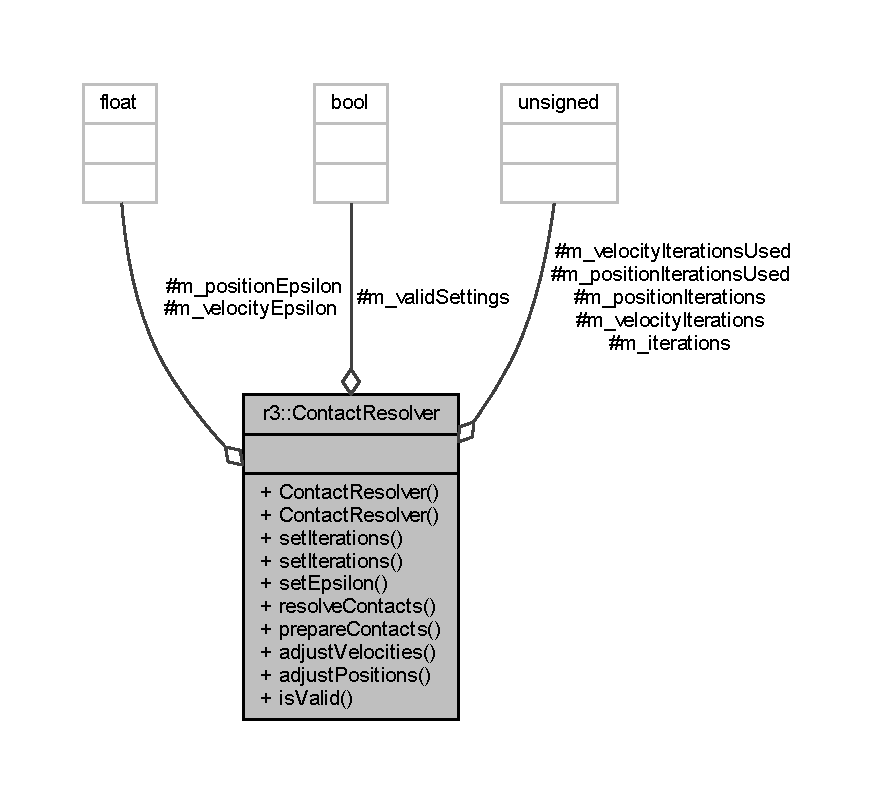
\includegraphics[width=350pt]{classr3_1_1_contact_resolver__coll__graph}
\end{center}
\end{figure}
\subsection*{Public Member Functions}
\begin{DoxyCompactItemize}
\item 
\mbox{\hyperlink{classr3_1_1_contact_resolver_a1728aa5f4a167b00b0c138f6aacf3206}{Contact\+Resolver}} (unsigned iterations, \mbox{\hyperlink{namespacer3_ab2016b3e3f743fb735afce242f0dc1eb}{real}} velocity\+Epsilon=\mbox{\hyperlink{namespacer3_ab2016b3e3f743fb735afce242f0dc1eb}{real}}(0.\+01f), real position\+Epsilon=real(0.\+01f))
\item 
\mbox{\hyperlink{classr3_1_1_contact_resolver_acb2f7f96722326346fbe0e54d05cfdc9}{Contact\+Resolver}} (unsigned velocity\+Iterations, unsigned position\+Iterations, \mbox{\hyperlink{namespacer3_ab2016b3e3f743fb735afce242f0dc1eb}{real}} velocity\+Epsilon=\mbox{\hyperlink{namespacer3_ab2016b3e3f743fb735afce242f0dc1eb}{real}}(0.\+01f), real position\+Epsilon=real(0.\+01f))
\item 
void \mbox{\hyperlink{classr3_1_1_contact_resolver_aba01b66ae9ff4b713b65142466d3f98d}{set\+Iterations}} (unsigned iterations)
\item 
void \mbox{\hyperlink{classr3_1_1_contact_resolver_a661c4b7d7ba2232f16691e159601401f}{set\+Iterations}} (unsigned velocity\+Iterations, unsigned position\+Iterations)
\item 
void \mbox{\hyperlink{classr3_1_1_contact_resolver_a699cd63e020c47c52223efa1494bdfae}{set\+Epsilon}} (\mbox{\hyperlink{namespacer3_ab2016b3e3f743fb735afce242f0dc1eb}{real}} velocity\+Epsilon, \mbox{\hyperlink{namespacer3_ab2016b3e3f743fb735afce242f0dc1eb}{real}} position\+Epsilon)
\item 
void \mbox{\hyperlink{classr3_1_1_contact_resolver_a3ec12f4cbf8b42e1d481a77173b664c1}{resolve\+Contacts}} (\mbox{\hyperlink{classr3_1_1_contact_old}{Contact\+Old}} $\ast$contacts, unsigned num\+Contacts, \mbox{\hyperlink{namespacer3_ab2016b3e3f743fb735afce242f0dc1eb}{real}} time\+Delta)
\item 
void \mbox{\hyperlink{classr3_1_1_contact_resolver_ac791c4cb45b46702014703c54cd97f0f}{prepare\+Contacts}} (\mbox{\hyperlink{classr3_1_1_contact_old}{Contact\+Old}} $\ast$contacts, unsigned num\+Contacts, \mbox{\hyperlink{namespacer3_ab2016b3e3f743fb735afce242f0dc1eb}{real}} time\+Delta)
\item 
void \mbox{\hyperlink{classr3_1_1_contact_resolver_aa5d26e400938482f47fd5efa760ea9d3}{adjust\+Velocities}} (\mbox{\hyperlink{classr3_1_1_contact_old}{Contact\+Old}} $\ast$c, unsigned num\+Contacts, \mbox{\hyperlink{namespacer3_ab2016b3e3f743fb735afce242f0dc1eb}{real}} time\+Delta)
\item 
void \mbox{\hyperlink{classr3_1_1_contact_resolver_a5dc41bad46cf659b93488f7c7db74712}{adjust\+Positions}} (\mbox{\hyperlink{classr3_1_1_contact_old}{Contact\+Old}} $\ast$c, unsigned num\+Contacts, \mbox{\hyperlink{namespacer3_ab2016b3e3f743fb735afce242f0dc1eb}{real}} time\+Delta)
\item 
bool \mbox{\hyperlink{classr3_1_1_contact_resolver_a7864d5856905dfc9b083931c891dddc6}{is\+Valid}} () const
\end{DoxyCompactItemize}
\subsection*{Protected Attributes}
\begin{DoxyCompactItemize}
\item 
unsigned \mbox{\hyperlink{classr3_1_1_contact_resolver_a5ebf50739d29cfd44c839f0949653f56}{m\+\_\+velocity\+Iterations}}
\item 
unsigned \mbox{\hyperlink{classr3_1_1_contact_resolver_a53bef5ef42c6f5d643b30888f517332d}{m\+\_\+position\+Iterations}}
\item 
\mbox{\hyperlink{namespacer3_ab2016b3e3f743fb735afce242f0dc1eb}{real}} \mbox{\hyperlink{classr3_1_1_contact_resolver_ae3aeb6defa615dfc0be6b0e9a79b1964}{m\+\_\+velocity\+Epsilon}}
\item 
\mbox{\hyperlink{namespacer3_ab2016b3e3f743fb735afce242f0dc1eb}{real}} \mbox{\hyperlink{classr3_1_1_contact_resolver_aea34f9f1d5131d0949878375e8eefff6}{m\+\_\+position\+Epsilon}}
\item 
unsigned \mbox{\hyperlink{classr3_1_1_contact_resolver_a1d02afed1bbae067eee7792fcb859278}{m\+\_\+velocity\+Iterations\+Used}}
\item 
unsigned \mbox{\hyperlink{classr3_1_1_contact_resolver_a4e790314254412d28d2063b1e0f26e4b}{m\+\_\+position\+Iterations\+Used}}
\item 
bool \mbox{\hyperlink{classr3_1_1_contact_resolver_a3015ece0b9280101a65abcc2b2b4c85f}{m\+\_\+valid\+Settings}}
\item 
unsigned \mbox{\hyperlink{classr3_1_1_contact_resolver_add8b2f230c8ed5ef56639dec4f111a44}{m\+\_\+iterations}}
\end{DoxyCompactItemize}


\subsection{Constructor \& Destructor Documentation}
\mbox{\Hypertarget{classr3_1_1_contact_resolver_a1728aa5f4a167b00b0c138f6aacf3206}\label{classr3_1_1_contact_resolver_a1728aa5f4a167b00b0c138f6aacf3206}} 
\index{r3\+::\+Contact\+Resolver@{r3\+::\+Contact\+Resolver}!Contact\+Resolver@{Contact\+Resolver}}
\index{Contact\+Resolver@{Contact\+Resolver}!r3\+::\+Contact\+Resolver@{r3\+::\+Contact\+Resolver}}
\subsubsection{\texorpdfstring{Contact\+Resolver()}{ContactResolver()}\hspace{0.1cm}{\footnotesize\ttfamily [1/2]}}
{\footnotesize\ttfamily r3\+::\+Contact\+Resolver\+::\+Contact\+Resolver (\begin{DoxyParamCaption}\item[{unsigned}]{iterations,  }\item[{\mbox{\hyperlink{namespacer3_ab2016b3e3f743fb735afce242f0dc1eb}{real}}}]{velocity\+Epsilon = {\ttfamily \mbox{\hyperlink{namespacer3_ab2016b3e3f743fb735afce242f0dc1eb}{real}}(0.01f)},  }\item[{\mbox{\hyperlink{namespacer3_ab2016b3e3f743fb735afce242f0dc1eb}{real}}}]{position\+Epsilon = {\ttfamily \mbox{\hyperlink{namespacer3_ab2016b3e3f743fb735afce242f0dc1eb}{real}}(0.01f)} }\end{DoxyParamCaption})\hspace{0.3cm}{\ttfamily [explicit]}}

Creates a new contact resolver with the given number of iterations per resolution call, and optional epsilon values. \mbox{\Hypertarget{classr3_1_1_contact_resolver_acb2f7f96722326346fbe0e54d05cfdc9}\label{classr3_1_1_contact_resolver_acb2f7f96722326346fbe0e54d05cfdc9}} 
\index{r3\+::\+Contact\+Resolver@{r3\+::\+Contact\+Resolver}!Contact\+Resolver@{Contact\+Resolver}}
\index{Contact\+Resolver@{Contact\+Resolver}!r3\+::\+Contact\+Resolver@{r3\+::\+Contact\+Resolver}}
\subsubsection{\texorpdfstring{Contact\+Resolver()}{ContactResolver()}\hspace{0.1cm}{\footnotesize\ttfamily [2/2]}}
{\footnotesize\ttfamily r3\+::\+Contact\+Resolver\+::\+Contact\+Resolver (\begin{DoxyParamCaption}\item[{unsigned}]{velocity\+Iterations,  }\item[{unsigned}]{position\+Iterations,  }\item[{\mbox{\hyperlink{namespacer3_ab2016b3e3f743fb735afce242f0dc1eb}{real}}}]{velocity\+Epsilon = {\ttfamily \mbox{\hyperlink{namespacer3_ab2016b3e3f743fb735afce242f0dc1eb}{real}}(0.01f)},  }\item[{\mbox{\hyperlink{namespacer3_ab2016b3e3f743fb735afce242f0dc1eb}{real}}}]{position\+Epsilon = {\ttfamily \mbox{\hyperlink{namespacer3_ab2016b3e3f743fb735afce242f0dc1eb}{real}}(0.01f)} }\end{DoxyParamCaption})}

Creates a new contact resolver with the given number of iterations for each kind of resolution, and optional epsilon values. 

\subsection{Member Function Documentation}
\mbox{\Hypertarget{classr3_1_1_contact_resolver_a5dc41bad46cf659b93488f7c7db74712}\label{classr3_1_1_contact_resolver_a5dc41bad46cf659b93488f7c7db74712}} 
\index{r3\+::\+Contact\+Resolver@{r3\+::\+Contact\+Resolver}!adjust\+Positions@{adjust\+Positions}}
\index{adjust\+Positions@{adjust\+Positions}!r3\+::\+Contact\+Resolver@{r3\+::\+Contact\+Resolver}}
\subsubsection{\texorpdfstring{adjust\+Positions()}{adjustPositions()}}
{\footnotesize\ttfamily void r3\+::\+Contact\+Resolver\+::adjust\+Positions (\begin{DoxyParamCaption}\item[{\mbox{\hyperlink{classr3_1_1_contact_old}{Contact\+Old}} $\ast$}]{c,  }\item[{unsigned}]{num\+Contacts,  }\item[{\mbox{\hyperlink{namespacer3_ab2016b3e3f743fb735afce242f0dc1eb}{real}}}]{time\+Delta }\end{DoxyParamCaption})}

\mbox{\Hypertarget{classr3_1_1_contact_resolver_aa5d26e400938482f47fd5efa760ea9d3}\label{classr3_1_1_contact_resolver_aa5d26e400938482f47fd5efa760ea9d3}} 
\index{r3\+::\+Contact\+Resolver@{r3\+::\+Contact\+Resolver}!adjust\+Velocities@{adjust\+Velocities}}
\index{adjust\+Velocities@{adjust\+Velocities}!r3\+::\+Contact\+Resolver@{r3\+::\+Contact\+Resolver}}
\subsubsection{\texorpdfstring{adjust\+Velocities()}{adjustVelocities()}}
{\footnotesize\ttfamily void r3\+::\+Contact\+Resolver\+::adjust\+Velocities (\begin{DoxyParamCaption}\item[{\mbox{\hyperlink{classr3_1_1_contact_old}{Contact\+Old}} $\ast$}]{c,  }\item[{unsigned}]{num\+Contacts,  }\item[{\mbox{\hyperlink{namespacer3_ab2016b3e3f743fb735afce242f0dc1eb}{real}}}]{time\+Delta }\end{DoxyParamCaption})}

\mbox{\Hypertarget{classr3_1_1_contact_resolver_a7864d5856905dfc9b083931c891dddc6}\label{classr3_1_1_contact_resolver_a7864d5856905dfc9b083931c891dddc6}} 
\index{r3\+::\+Contact\+Resolver@{r3\+::\+Contact\+Resolver}!is\+Valid@{is\+Valid}}
\index{is\+Valid@{is\+Valid}!r3\+::\+Contact\+Resolver@{r3\+::\+Contact\+Resolver}}
\subsubsection{\texorpdfstring{is\+Valid()}{isValid()}}
{\footnotesize\ttfamily bool r3\+::\+Contact\+Resolver\+::is\+Valid (\begin{DoxyParamCaption}{ }\end{DoxyParamCaption}) const}

\mbox{\Hypertarget{classr3_1_1_contact_resolver_ac791c4cb45b46702014703c54cd97f0f}\label{classr3_1_1_contact_resolver_ac791c4cb45b46702014703c54cd97f0f}} 
\index{r3\+::\+Contact\+Resolver@{r3\+::\+Contact\+Resolver}!prepare\+Contacts@{prepare\+Contacts}}
\index{prepare\+Contacts@{prepare\+Contacts}!r3\+::\+Contact\+Resolver@{r3\+::\+Contact\+Resolver}}
\subsubsection{\texorpdfstring{prepare\+Contacts()}{prepareContacts()}}
{\footnotesize\ttfamily void r3\+::\+Contact\+Resolver\+::prepare\+Contacts (\begin{DoxyParamCaption}\item[{\mbox{\hyperlink{classr3_1_1_contact_old}{Contact\+Old}} $\ast$}]{contacts,  }\item[{unsigned}]{num\+Contacts,  }\item[{\mbox{\hyperlink{namespacer3_ab2016b3e3f743fb735afce242f0dc1eb}{real}}}]{time\+Delta }\end{DoxyParamCaption})}

\mbox{\Hypertarget{classr3_1_1_contact_resolver_a3ec12f4cbf8b42e1d481a77173b664c1}\label{classr3_1_1_contact_resolver_a3ec12f4cbf8b42e1d481a77173b664c1}} 
\index{r3\+::\+Contact\+Resolver@{r3\+::\+Contact\+Resolver}!resolve\+Contacts@{resolve\+Contacts}}
\index{resolve\+Contacts@{resolve\+Contacts}!r3\+::\+Contact\+Resolver@{r3\+::\+Contact\+Resolver}}
\subsubsection{\texorpdfstring{resolve\+Contacts()}{resolveContacts()}}
{\footnotesize\ttfamily void r3\+::\+Contact\+Resolver\+::resolve\+Contacts (\begin{DoxyParamCaption}\item[{\mbox{\hyperlink{classr3_1_1_contact_old}{Contact\+Old}} $\ast$}]{contacts,  }\item[{unsigned}]{num\+Contacts,  }\item[{\mbox{\hyperlink{namespacer3_ab2016b3e3f743fb735afce242f0dc1eb}{real}}}]{time\+Delta }\end{DoxyParamCaption})}

\mbox{\Hypertarget{classr3_1_1_contact_resolver_a699cd63e020c47c52223efa1494bdfae}\label{classr3_1_1_contact_resolver_a699cd63e020c47c52223efa1494bdfae}} 
\index{r3\+::\+Contact\+Resolver@{r3\+::\+Contact\+Resolver}!set\+Epsilon@{set\+Epsilon}}
\index{set\+Epsilon@{set\+Epsilon}!r3\+::\+Contact\+Resolver@{r3\+::\+Contact\+Resolver}}
\subsubsection{\texorpdfstring{set\+Epsilon()}{setEpsilon()}}
{\footnotesize\ttfamily void r3\+::\+Contact\+Resolver\+::set\+Epsilon (\begin{DoxyParamCaption}\item[{\mbox{\hyperlink{namespacer3_ab2016b3e3f743fb735afce242f0dc1eb}{real}}}]{velocity\+Epsilon,  }\item[{\mbox{\hyperlink{namespacer3_ab2016b3e3f743fb735afce242f0dc1eb}{real}}}]{position\+Epsilon }\end{DoxyParamCaption})}

\mbox{\Hypertarget{classr3_1_1_contact_resolver_aba01b66ae9ff4b713b65142466d3f98d}\label{classr3_1_1_contact_resolver_aba01b66ae9ff4b713b65142466d3f98d}} 
\index{r3\+::\+Contact\+Resolver@{r3\+::\+Contact\+Resolver}!set\+Iterations@{set\+Iterations}}
\index{set\+Iterations@{set\+Iterations}!r3\+::\+Contact\+Resolver@{r3\+::\+Contact\+Resolver}}
\subsubsection{\texorpdfstring{set\+Iterations()}{setIterations()}\hspace{0.1cm}{\footnotesize\ttfamily [1/2]}}
{\footnotesize\ttfamily void r3\+::\+Contact\+Resolver\+::set\+Iterations (\begin{DoxyParamCaption}\item[{unsigned}]{iterations }\end{DoxyParamCaption})}

\mbox{\Hypertarget{classr3_1_1_contact_resolver_a661c4b7d7ba2232f16691e159601401f}\label{classr3_1_1_contact_resolver_a661c4b7d7ba2232f16691e159601401f}} 
\index{r3\+::\+Contact\+Resolver@{r3\+::\+Contact\+Resolver}!set\+Iterations@{set\+Iterations}}
\index{set\+Iterations@{set\+Iterations}!r3\+::\+Contact\+Resolver@{r3\+::\+Contact\+Resolver}}
\subsubsection{\texorpdfstring{set\+Iterations()}{setIterations()}\hspace{0.1cm}{\footnotesize\ttfamily [2/2]}}
{\footnotesize\ttfamily void r3\+::\+Contact\+Resolver\+::set\+Iterations (\begin{DoxyParamCaption}\item[{unsigned}]{velocity\+Iterations,  }\item[{unsigned}]{position\+Iterations }\end{DoxyParamCaption})}



\subsection{Member Data Documentation}
\mbox{\Hypertarget{classr3_1_1_contact_resolver_add8b2f230c8ed5ef56639dec4f111a44}\label{classr3_1_1_contact_resolver_add8b2f230c8ed5ef56639dec4f111a44}} 
\index{r3\+::\+Contact\+Resolver@{r3\+::\+Contact\+Resolver}!m\+\_\+iterations@{m\+\_\+iterations}}
\index{m\+\_\+iterations@{m\+\_\+iterations}!r3\+::\+Contact\+Resolver@{r3\+::\+Contact\+Resolver}}
\subsubsection{\texorpdfstring{m\+\_\+iterations}{m\_iterations}}
{\footnotesize\ttfamily unsigned r3\+::\+Contact\+Resolver\+::m\+\_\+iterations\hspace{0.3cm}{\ttfamily [protected]}}

\mbox{\Hypertarget{classr3_1_1_contact_resolver_aea34f9f1d5131d0949878375e8eefff6}\label{classr3_1_1_contact_resolver_aea34f9f1d5131d0949878375e8eefff6}} 
\index{r3\+::\+Contact\+Resolver@{r3\+::\+Contact\+Resolver}!m\+\_\+position\+Epsilon@{m\+\_\+position\+Epsilon}}
\index{m\+\_\+position\+Epsilon@{m\+\_\+position\+Epsilon}!r3\+::\+Contact\+Resolver@{r3\+::\+Contact\+Resolver}}
\subsubsection{\texorpdfstring{m\+\_\+position\+Epsilon}{m\_positionEpsilon}}
{\footnotesize\ttfamily \mbox{\hyperlink{namespacer3_ab2016b3e3f743fb735afce242f0dc1eb}{real}} r3\+::\+Contact\+Resolver\+::m\+\_\+position\+Epsilon\hspace{0.3cm}{\ttfamily [protected]}}

To avoid instability penetrations smaller than this value are considered to be not interpenetrating. Too small and the simulation may be unstable, too large and the bodies may interpenetrate visually. A good starting point is the default of0.\+01. \mbox{\Hypertarget{classr3_1_1_contact_resolver_a53bef5ef42c6f5d643b30888f517332d}\label{classr3_1_1_contact_resolver_a53bef5ef42c6f5d643b30888f517332d}} 
\index{r3\+::\+Contact\+Resolver@{r3\+::\+Contact\+Resolver}!m\+\_\+position\+Iterations@{m\+\_\+position\+Iterations}}
\index{m\+\_\+position\+Iterations@{m\+\_\+position\+Iterations}!r3\+::\+Contact\+Resolver@{r3\+::\+Contact\+Resolver}}
\subsubsection{\texorpdfstring{m\+\_\+position\+Iterations}{m\_positionIterations}}
{\footnotesize\ttfamily unsigned r3\+::\+Contact\+Resolver\+::m\+\_\+position\+Iterations\hspace{0.3cm}{\ttfamily [protected]}}

Holds the number of iterations to perform when resolving position. \mbox{\Hypertarget{classr3_1_1_contact_resolver_a4e790314254412d28d2063b1e0f26e4b}\label{classr3_1_1_contact_resolver_a4e790314254412d28d2063b1e0f26e4b}} 
\index{r3\+::\+Contact\+Resolver@{r3\+::\+Contact\+Resolver}!m\+\_\+position\+Iterations\+Used@{m\+\_\+position\+Iterations\+Used}}
\index{m\+\_\+position\+Iterations\+Used@{m\+\_\+position\+Iterations\+Used}!r3\+::\+Contact\+Resolver@{r3\+::\+Contact\+Resolver}}
\subsubsection{\texorpdfstring{m\+\_\+position\+Iterations\+Used}{m\_positionIterationsUsed}}
{\footnotesize\ttfamily unsigned r3\+::\+Contact\+Resolver\+::m\+\_\+position\+Iterations\+Used\hspace{0.3cm}{\ttfamily [protected]}}

Stores the number of position iterations used in the last call to resolve contacts. \mbox{\Hypertarget{classr3_1_1_contact_resolver_a3015ece0b9280101a65abcc2b2b4c85f}\label{classr3_1_1_contact_resolver_a3015ece0b9280101a65abcc2b2b4c85f}} 
\index{r3\+::\+Contact\+Resolver@{r3\+::\+Contact\+Resolver}!m\+\_\+valid\+Settings@{m\+\_\+valid\+Settings}}
\index{m\+\_\+valid\+Settings@{m\+\_\+valid\+Settings}!r3\+::\+Contact\+Resolver@{r3\+::\+Contact\+Resolver}}
\subsubsection{\texorpdfstring{m\+\_\+valid\+Settings}{m\_validSettings}}
{\footnotesize\ttfamily bool r3\+::\+Contact\+Resolver\+::m\+\_\+valid\+Settings\hspace{0.3cm}{\ttfamily [protected]}}

Keeps track of whether the internal settings are valid. \mbox{\Hypertarget{classr3_1_1_contact_resolver_ae3aeb6defa615dfc0be6b0e9a79b1964}\label{classr3_1_1_contact_resolver_ae3aeb6defa615dfc0be6b0e9a79b1964}} 
\index{r3\+::\+Contact\+Resolver@{r3\+::\+Contact\+Resolver}!m\+\_\+velocity\+Epsilon@{m\+\_\+velocity\+Epsilon}}
\index{m\+\_\+velocity\+Epsilon@{m\+\_\+velocity\+Epsilon}!r3\+::\+Contact\+Resolver@{r3\+::\+Contact\+Resolver}}
\subsubsection{\texorpdfstring{m\+\_\+velocity\+Epsilon}{m\_velocityEpsilon}}
{\footnotesize\ttfamily \mbox{\hyperlink{namespacer3_ab2016b3e3f743fb735afce242f0dc1eb}{real}} r3\+::\+Contact\+Resolver\+::m\+\_\+velocity\+Epsilon\hspace{0.3cm}{\ttfamily [protected]}}

To avoid instability velocities smaller than this value are considered to be zero. Too small and the simulation may be unstable, too large and the bodies may interpenetrate visually. A good starting point is the default of 0.\+01. \mbox{\Hypertarget{classr3_1_1_contact_resolver_a5ebf50739d29cfd44c839f0949653f56}\label{classr3_1_1_contact_resolver_a5ebf50739d29cfd44c839f0949653f56}} 
\index{r3\+::\+Contact\+Resolver@{r3\+::\+Contact\+Resolver}!m\+\_\+velocity\+Iterations@{m\+\_\+velocity\+Iterations}}
\index{m\+\_\+velocity\+Iterations@{m\+\_\+velocity\+Iterations}!r3\+::\+Contact\+Resolver@{r3\+::\+Contact\+Resolver}}
\subsubsection{\texorpdfstring{m\+\_\+velocity\+Iterations}{m\_velocityIterations}}
{\footnotesize\ttfamily unsigned r3\+::\+Contact\+Resolver\+::m\+\_\+velocity\+Iterations\hspace{0.3cm}{\ttfamily [protected]}}

Holds the number of iterations to perform when resolving velocity. \mbox{\Hypertarget{classr3_1_1_contact_resolver_a1d02afed1bbae067eee7792fcb859278}\label{classr3_1_1_contact_resolver_a1d02afed1bbae067eee7792fcb859278}} 
\index{r3\+::\+Contact\+Resolver@{r3\+::\+Contact\+Resolver}!m\+\_\+velocity\+Iterations\+Used@{m\+\_\+velocity\+Iterations\+Used}}
\index{m\+\_\+velocity\+Iterations\+Used@{m\+\_\+velocity\+Iterations\+Used}!r3\+::\+Contact\+Resolver@{r3\+::\+Contact\+Resolver}}
\subsubsection{\texorpdfstring{m\+\_\+velocity\+Iterations\+Used}{m\_velocityIterationsUsed}}
{\footnotesize\ttfamily unsigned r3\+::\+Contact\+Resolver\+::m\+\_\+velocity\+Iterations\+Used\hspace{0.3cm}{\ttfamily [protected]}}

Stores the number of velocity iterations used in the last call to resolve contacts. 

The documentation for this class was generated from the following files\+:\begin{DoxyCompactItemize}
\item 
D\+:/\+Library/\+Documents/\+Job/\+Forschungsmaster/\+Projekte/\+Simulation\+Visualization/\+Rumble3\+D/\+Rumble3\+D/include/\+R3\+D/\+Rigid\+Body\+Engine/\mbox{\hyperlink{_contact_resolver_8h}{Contact\+Resolver.\+h}}\item 
D\+:/\+Library/\+Documents/\+Job/\+Forschungsmaster/\+Projekte/\+Simulation\+Visualization/\+Rumble3\+D/\+Rumble3\+D/src/\+Rigid\+Body\+Engine/\mbox{\hyperlink{_contact_resolver_8cpp}{Contact\+Resolver.\+cpp}}\end{DoxyCompactItemize}

\hypertarget{classr3_1_1_default_particle_engine_c_i}{}\section{r3\+:\+:Default\+Particle\+Engine\+CI Class Reference}
\label{classr3_1_1_default_particle_engine_c_i}\index{r3\+::\+Default\+Particle\+Engine\+CI@{r3\+::\+Default\+Particle\+Engine\+CI}}


Default implementation of the particle computation interface.  




{\ttfamily \#include $<$Default\+Particle\+Engine\+C\+I.\+h$>$}



Inheritance diagram for r3\+:\+:Default\+Particle\+Engine\+CI\+:\nopagebreak
\begin{figure}[H]
\begin{center}
\leavevmode
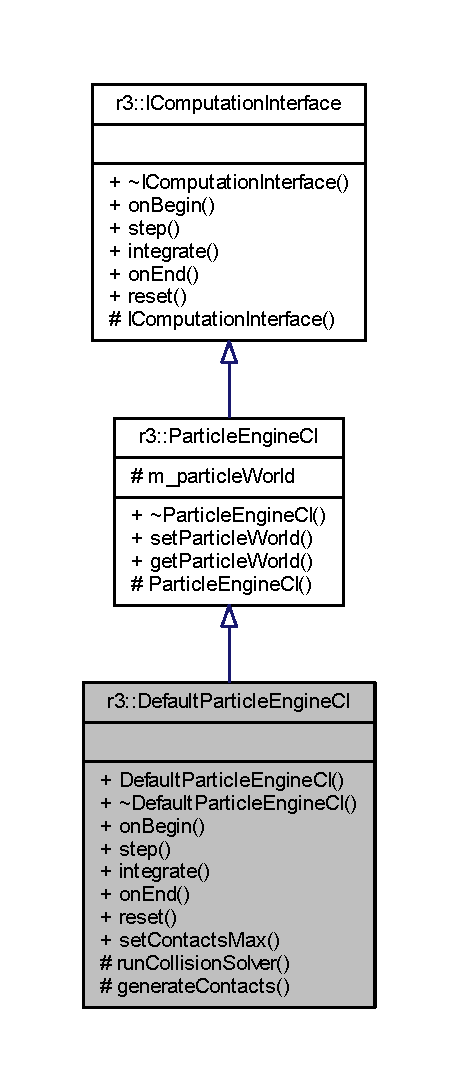
\includegraphics[width=220pt]{classr3_1_1_default_particle_engine_c_i__inherit__graph}
\end{center}
\end{figure}


Collaboration diagram for r3\+:\+:Default\+Particle\+Engine\+CI\+:\nopagebreak
\begin{figure}[H]
\begin{center}
\leavevmode
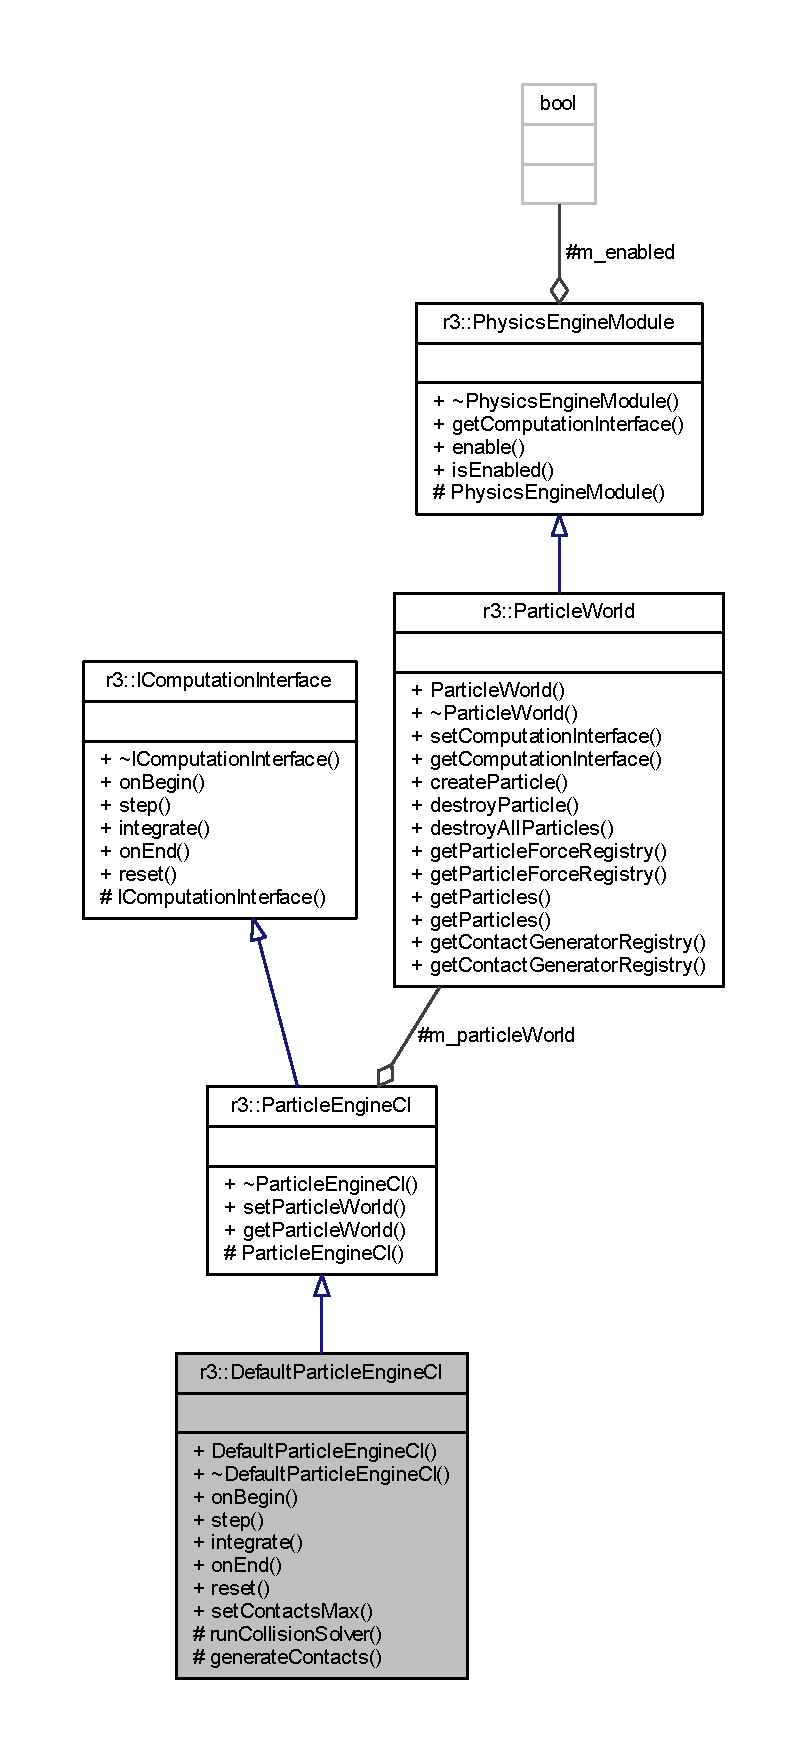
\includegraphics[height=550pt]{classr3_1_1_default_particle_engine_c_i__coll__graph}
\end{center}
\end{figure}
\subsection*{Public Member Functions}
\begin{DoxyCompactItemize}
\item 
\mbox{\hyperlink{classr3_1_1_default_particle_engine_c_i_a5f7619a5dd227d681d5dcbde6e8368eb}{Default\+Particle\+Engine\+CI}} (unsigned contacts\+Max, unsigned iterations=0, \mbox{\hyperlink{classr3_1_1_particle_world}{Particle\+World}} $\ast$particle\+World=nullptr)
\begin{DoxyCompactList}\small\item\em \mbox{\hyperlink{classr3_1_1_default_particle_engine_c_i}{Default\+Particle\+Engine\+CI}} constructor. \end{DoxyCompactList}\item 
\mbox{\hyperlink{classr3_1_1_default_particle_engine_c_i_afb7df43eb7fe45d6bcb15c39e3c30849}{$\sim$\+Default\+Particle\+Engine\+CI}} ()
\item 
void \mbox{\hyperlink{classr3_1_1_default_particle_engine_c_i_aaf2e9ca87bff5e48c8eb59384e9cf180}{on\+Begin}} () override
\item 
void \mbox{\hyperlink{classr3_1_1_default_particle_engine_c_i_a7c58fd00ec521410e1b412e9885ee0d2}{step}} (\mbox{\hyperlink{namespacer3_ab2016b3e3f743fb735afce242f0dc1eb}{real}} time\+Delta) override
\begin{DoxyCompactList}\small\item\em Update particle forces. \end{DoxyCompactList}\item 
void \mbox{\hyperlink{classr3_1_1_default_particle_engine_c_i_a4603707afe6c841a83294a46ea4a1c62}{integrate}} (\mbox{\hyperlink{namespacer3_ab2016b3e3f743fb735afce242f0dc1eb}{real}} time\+Delta) override
\begin{DoxyCompactList}\small\item\em Perform integration and solve collisions. \end{DoxyCompactList}\item 
void \mbox{\hyperlink{classr3_1_1_default_particle_engine_c_i_a6a34c77436d8133560eaa7366c740119}{on\+End}} () override
\begin{DoxyCompactList}\small\item\em Clear force accumulators and reset contact data. \end{DoxyCompactList}\item 
void \mbox{\hyperlink{classr3_1_1_default_particle_engine_c_i_a97757c62b4cb1266da29e2b5625bb9d3}{reset}} () override
\begin{DoxyCompactList}\small\item\em Reset the computation interface. \end{DoxyCompactList}\item 
void \mbox{\hyperlink{classr3_1_1_default_particle_engine_c_i_a7dbb49cbf2f5b028656ea2e14174a3ed}{set\+Contacts\+Max}} (unsigned contacts\+Max)
\begin{DoxyCompactList}\small\item\em Set the maximal number of contacts that the collision solver can use. \end{DoxyCompactList}\end{DoxyCompactItemize}
\subsection*{Protected Member Functions}
\begin{DoxyCompactItemize}
\item 
void \mbox{\hyperlink{classr3_1_1_default_particle_engine_c_i_a19138f7707e948b7e8e05647bcba52fe}{run\+Collision\+Solver}} (\mbox{\hyperlink{namespacer3_ab2016b3e3f743fb735afce242f0dc1eb}{real}} time\+Delta)
\begin{DoxyCompactList}\small\item\em Solve all previously generated particle contacts. \end{DoxyCompactList}\item 
void \mbox{\hyperlink{classr3_1_1_default_particle_engine_c_i_a61aea4f32cc73960915d3c68396bd47e}{generate\+Contacts}} ()
\begin{DoxyCompactList}\small\item\em Generate particle contacts by using all registered particle contact generators. \end{DoxyCompactList}\end{DoxyCompactItemize}
\subsection*{Additional Inherited Members}


\subsection{Detailed Description}
Default implementation of the particle computation interface. 

\subsection{Constructor \& Destructor Documentation}
\mbox{\Hypertarget{classr3_1_1_default_particle_engine_c_i_a5f7619a5dd227d681d5dcbde6e8368eb}\label{classr3_1_1_default_particle_engine_c_i_a5f7619a5dd227d681d5dcbde6e8368eb}} 
\index{r3\+::\+Default\+Particle\+Engine\+CI@{r3\+::\+Default\+Particle\+Engine\+CI}!Default\+Particle\+Engine\+CI@{Default\+Particle\+Engine\+CI}}
\index{Default\+Particle\+Engine\+CI@{Default\+Particle\+Engine\+CI}!r3\+::\+Default\+Particle\+Engine\+CI@{r3\+::\+Default\+Particle\+Engine\+CI}}
\subsubsection{\texorpdfstring{Default\+Particle\+Engine\+C\+I()}{DefaultParticleEngineCI()}}
{\footnotesize\ttfamily r3\+::\+Default\+Particle\+Engine\+C\+I\+::\+Default\+Particle\+Engine\+CI (\begin{DoxyParamCaption}\item[{unsigned}]{contacts\+Max,  }\item[{unsigned}]{iterations = {\ttfamily 0},  }\item[{\mbox{\hyperlink{classr3_1_1_particle_world}{Particle\+World}} $\ast$}]{particle\+World = {\ttfamily nullptr} }\end{DoxyParamCaption})\hspace{0.3cm}{\ttfamily [explicit]}}



\mbox{\hyperlink{classr3_1_1_default_particle_engine_c_i}{Default\+Particle\+Engine\+CI}} constructor. 


\begin{DoxyParams}{Parameters}
{\em contacts\+Max} & Maximal number of contacts, which can exist at the same time. \\
\hline
{\em iterations} & Maximal number of iterations the particle contact generator can use. \\
\hline
{\em particle\+World} & The particle world, which should be used for calculations. \\
\hline
\end{DoxyParams}
\mbox{\Hypertarget{classr3_1_1_default_particle_engine_c_i_afb7df43eb7fe45d6bcb15c39e3c30849}\label{classr3_1_1_default_particle_engine_c_i_afb7df43eb7fe45d6bcb15c39e3c30849}} 
\index{r3\+::\+Default\+Particle\+Engine\+CI@{r3\+::\+Default\+Particle\+Engine\+CI}!````~Default\+Particle\+Engine\+CI@{$\sim$\+Default\+Particle\+Engine\+CI}}
\index{````~Default\+Particle\+Engine\+CI@{$\sim$\+Default\+Particle\+Engine\+CI}!r3\+::\+Default\+Particle\+Engine\+CI@{r3\+::\+Default\+Particle\+Engine\+CI}}
\subsubsection{\texorpdfstring{$\sim$\+Default\+Particle\+Engine\+C\+I()}{~DefaultParticleEngineCI()}}
{\footnotesize\ttfamily r3\+::\+Default\+Particle\+Engine\+C\+I\+::$\sim$\+Default\+Particle\+Engine\+CI (\begin{DoxyParamCaption}{ }\end{DoxyParamCaption})\hspace{0.3cm}{\ttfamily [default]}}



\subsection{Member Function Documentation}
\mbox{\Hypertarget{classr3_1_1_default_particle_engine_c_i_a61aea4f32cc73960915d3c68396bd47e}\label{classr3_1_1_default_particle_engine_c_i_a61aea4f32cc73960915d3c68396bd47e}} 
\index{r3\+::\+Default\+Particle\+Engine\+CI@{r3\+::\+Default\+Particle\+Engine\+CI}!generate\+Contacts@{generate\+Contacts}}
\index{generate\+Contacts@{generate\+Contacts}!r3\+::\+Default\+Particle\+Engine\+CI@{r3\+::\+Default\+Particle\+Engine\+CI}}
\subsubsection{\texorpdfstring{generate\+Contacts()}{generateContacts()}}
{\footnotesize\ttfamily void r3\+::\+Default\+Particle\+Engine\+C\+I\+::generate\+Contacts (\begin{DoxyParamCaption}{ }\end{DoxyParamCaption})\hspace{0.3cm}{\ttfamily [protected]}}



Generate particle contacts by using all registered particle contact generators. 

\mbox{\Hypertarget{classr3_1_1_default_particle_engine_c_i_a4603707afe6c841a83294a46ea4a1c62}\label{classr3_1_1_default_particle_engine_c_i_a4603707afe6c841a83294a46ea4a1c62}} 
\index{r3\+::\+Default\+Particle\+Engine\+CI@{r3\+::\+Default\+Particle\+Engine\+CI}!integrate@{integrate}}
\index{integrate@{integrate}!r3\+::\+Default\+Particle\+Engine\+CI@{r3\+::\+Default\+Particle\+Engine\+CI}}
\subsubsection{\texorpdfstring{integrate()}{integrate()}}
{\footnotesize\ttfamily void r3\+::\+Default\+Particle\+Engine\+C\+I\+::integrate (\begin{DoxyParamCaption}\item[{\mbox{\hyperlink{namespacer3_ab2016b3e3f743fb735afce242f0dc1eb}{real}}}]{time\+Delta }\end{DoxyParamCaption})\hspace{0.3cm}{\ttfamily [override]}, {\ttfamily [virtual]}}



Perform integration and solve collisions. 


\begin{DoxyParams}{Parameters}
{\em time\+Delta} & Time step of this update. \\
\hline
\end{DoxyParams}


Implements \mbox{\hyperlink{classr3_1_1_i_computation_interface_a162250f2b6efbd85460bd0f780d42cff}{r3\+::\+I\+Computation\+Interface}}.

\mbox{\Hypertarget{classr3_1_1_default_particle_engine_c_i_aaf2e9ca87bff5e48c8eb59384e9cf180}\label{classr3_1_1_default_particle_engine_c_i_aaf2e9ca87bff5e48c8eb59384e9cf180}} 
\index{r3\+::\+Default\+Particle\+Engine\+CI@{r3\+::\+Default\+Particle\+Engine\+CI}!on\+Begin@{on\+Begin}}
\index{on\+Begin@{on\+Begin}!r3\+::\+Default\+Particle\+Engine\+CI@{r3\+::\+Default\+Particle\+Engine\+CI}}
\subsubsection{\texorpdfstring{on\+Begin()}{onBegin()}}
{\footnotesize\ttfamily void r3\+::\+Default\+Particle\+Engine\+C\+I\+::on\+Begin (\begin{DoxyParamCaption}{ }\end{DoxyParamCaption})\hspace{0.3cm}{\ttfamily [override]}, {\ttfamily [virtual]}}



Implements \mbox{\hyperlink{classr3_1_1_i_computation_interface_a430ebc9cb8d4ba064ac6a032ef07edd7}{r3\+::\+I\+Computation\+Interface}}.

\mbox{\Hypertarget{classr3_1_1_default_particle_engine_c_i_a6a34c77436d8133560eaa7366c740119}\label{classr3_1_1_default_particle_engine_c_i_a6a34c77436d8133560eaa7366c740119}} 
\index{r3\+::\+Default\+Particle\+Engine\+CI@{r3\+::\+Default\+Particle\+Engine\+CI}!on\+End@{on\+End}}
\index{on\+End@{on\+End}!r3\+::\+Default\+Particle\+Engine\+CI@{r3\+::\+Default\+Particle\+Engine\+CI}}
\subsubsection{\texorpdfstring{on\+End()}{onEnd()}}
{\footnotesize\ttfamily void r3\+::\+Default\+Particle\+Engine\+C\+I\+::on\+End (\begin{DoxyParamCaption}{ }\end{DoxyParamCaption})\hspace{0.3cm}{\ttfamily [override]}, {\ttfamily [virtual]}}



Clear force accumulators and reset contact data. 



Implements \mbox{\hyperlink{classr3_1_1_i_computation_interface_acae0c5fada7e414c74fe6f5a8f4a6c7d}{r3\+::\+I\+Computation\+Interface}}.

\mbox{\Hypertarget{classr3_1_1_default_particle_engine_c_i_a97757c62b4cb1266da29e2b5625bb9d3}\label{classr3_1_1_default_particle_engine_c_i_a97757c62b4cb1266da29e2b5625bb9d3}} 
\index{r3\+::\+Default\+Particle\+Engine\+CI@{r3\+::\+Default\+Particle\+Engine\+CI}!reset@{reset}}
\index{reset@{reset}!r3\+::\+Default\+Particle\+Engine\+CI@{r3\+::\+Default\+Particle\+Engine\+CI}}
\subsubsection{\texorpdfstring{reset()}{reset()}}
{\footnotesize\ttfamily void r3\+::\+Default\+Particle\+Engine\+C\+I\+::reset (\begin{DoxyParamCaption}{ }\end{DoxyParamCaption})\hspace{0.3cm}{\ttfamily [override]}, {\ttfamily [virtual]}}



Reset the computation interface. 



Implements \mbox{\hyperlink{classr3_1_1_i_computation_interface_a6069989c54ffd4e714788d0968851007}{r3\+::\+I\+Computation\+Interface}}.

\mbox{\Hypertarget{classr3_1_1_default_particle_engine_c_i_a19138f7707e948b7e8e05647bcba52fe}\label{classr3_1_1_default_particle_engine_c_i_a19138f7707e948b7e8e05647bcba52fe}} 
\index{r3\+::\+Default\+Particle\+Engine\+CI@{r3\+::\+Default\+Particle\+Engine\+CI}!run\+Collision\+Solver@{run\+Collision\+Solver}}
\index{run\+Collision\+Solver@{run\+Collision\+Solver}!r3\+::\+Default\+Particle\+Engine\+CI@{r3\+::\+Default\+Particle\+Engine\+CI}}
\subsubsection{\texorpdfstring{run\+Collision\+Solver()}{runCollisionSolver()}}
{\footnotesize\ttfamily void r3\+::\+Default\+Particle\+Engine\+C\+I\+::run\+Collision\+Solver (\begin{DoxyParamCaption}\item[{\mbox{\hyperlink{namespacer3_ab2016b3e3f743fb735afce242f0dc1eb}{real}}}]{time\+Delta }\end{DoxyParamCaption})\hspace{0.3cm}{\ttfamily [protected]}}



Solve all previously generated particle contacts. 

\mbox{\Hypertarget{classr3_1_1_default_particle_engine_c_i_a7dbb49cbf2f5b028656ea2e14174a3ed}\label{classr3_1_1_default_particle_engine_c_i_a7dbb49cbf2f5b028656ea2e14174a3ed}} 
\index{r3\+::\+Default\+Particle\+Engine\+CI@{r3\+::\+Default\+Particle\+Engine\+CI}!set\+Contacts\+Max@{set\+Contacts\+Max}}
\index{set\+Contacts\+Max@{set\+Contacts\+Max}!r3\+::\+Default\+Particle\+Engine\+CI@{r3\+::\+Default\+Particle\+Engine\+CI}}
\subsubsection{\texorpdfstring{set\+Contacts\+Max()}{setContactsMax()}}
{\footnotesize\ttfamily void r3\+::\+Default\+Particle\+Engine\+C\+I\+::set\+Contacts\+Max (\begin{DoxyParamCaption}\item[{unsigned}]{contacts\+Max }\end{DoxyParamCaption})}



Set the maximal number of contacts that the collision solver can use. 


\begin{DoxyParams}{Parameters}
{\em contacts\+Max} & The maximal number of contacts. \\
\hline
\end{DoxyParams}
\mbox{\Hypertarget{classr3_1_1_default_particle_engine_c_i_a7c58fd00ec521410e1b412e9885ee0d2}\label{classr3_1_1_default_particle_engine_c_i_a7c58fd00ec521410e1b412e9885ee0d2}} 
\index{r3\+::\+Default\+Particle\+Engine\+CI@{r3\+::\+Default\+Particle\+Engine\+CI}!step@{step}}
\index{step@{step}!r3\+::\+Default\+Particle\+Engine\+CI@{r3\+::\+Default\+Particle\+Engine\+CI}}
\subsubsection{\texorpdfstring{step()}{step()}}
{\footnotesize\ttfamily void r3\+::\+Default\+Particle\+Engine\+C\+I\+::step (\begin{DoxyParamCaption}\item[{\mbox{\hyperlink{namespacer3_ab2016b3e3f743fb735afce242f0dc1eb}{real}}}]{time\+Delta }\end{DoxyParamCaption})\hspace{0.3cm}{\ttfamily [override]}, {\ttfamily [virtual]}}



Update particle forces. 


\begin{DoxyParams}{Parameters}
{\em time\+Delta} & Time step of this update. \\
\hline
\end{DoxyParams}


Implements \mbox{\hyperlink{classr3_1_1_i_computation_interface_aaa12bcc35005f32a1984b38de97696cb}{r3\+::\+I\+Computation\+Interface}}.



The documentation for this class was generated from the following files\+:\begin{DoxyCompactItemize}
\item 
D\+:/\+Library/\+Documents/\+Job/\+Forschungsmaster/\+Projekte/\+Simulation\+Visualization/\+Rumble3\+D/\+Rumble3\+D/include/\+R3\+D/\+Particle\+Engine/\mbox{\hyperlink{_default_particle_engine_c_i_8h}{Default\+Particle\+Engine\+C\+I.\+h}}\item 
D\+:/\+Library/\+Documents/\+Job/\+Forschungsmaster/\+Projekte/\+Simulation\+Visualization/\+Rumble3\+D/\+Rumble3\+D/src/\+Particle\+Engine/\mbox{\hyperlink{_default_particle_engine_c_i_8cpp}{Default\+Particle\+Engine\+C\+I.\+cpp}}\end{DoxyCompactItemize}

\hypertarget{classr3_1_1_default_rigid_body_engine_c_i}{}\section{r3\+:\+:Default\+Rigid\+Body\+Engine\+CI Class Reference}
\label{classr3_1_1_default_rigid_body_engine_c_i}\index{r3\+::\+Default\+Rigid\+Body\+Engine\+CI@{r3\+::\+Default\+Rigid\+Body\+Engine\+CI}}


Default implementation of the rigid body engine computation interface.  




{\ttfamily \#include $<$Default\+Rigid\+Body\+Engine\+C\+I.\+h$>$}



Inheritance diagram for r3\+:\+:Default\+Rigid\+Body\+Engine\+CI\+:\nopagebreak
\begin{figure}[H]
\begin{center}
\leavevmode
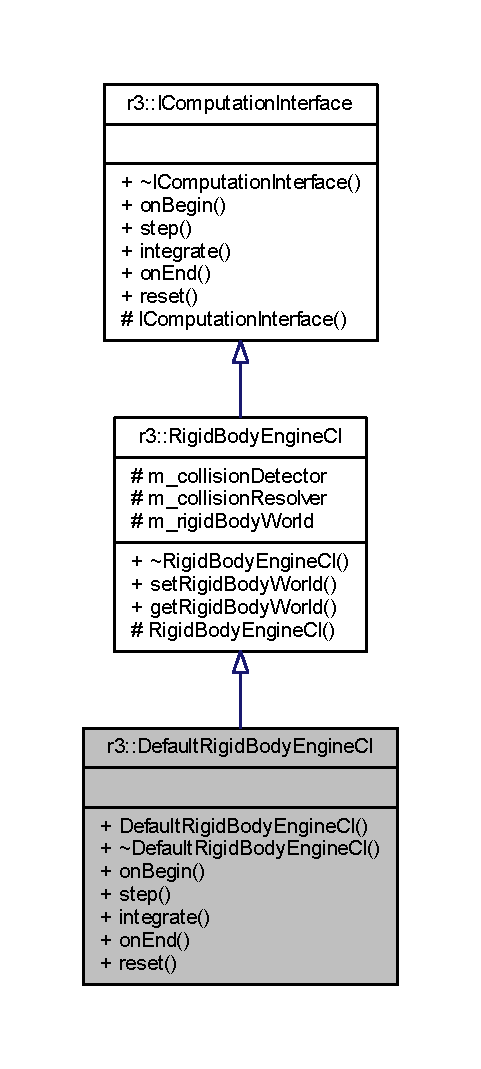
\includegraphics[width=231pt]{classr3_1_1_default_rigid_body_engine_c_i__inherit__graph}
\end{center}
\end{figure}


Collaboration diagram for r3\+:\+:Default\+Rigid\+Body\+Engine\+CI\+:\nopagebreak
\begin{figure}[H]
\begin{center}
\leavevmode
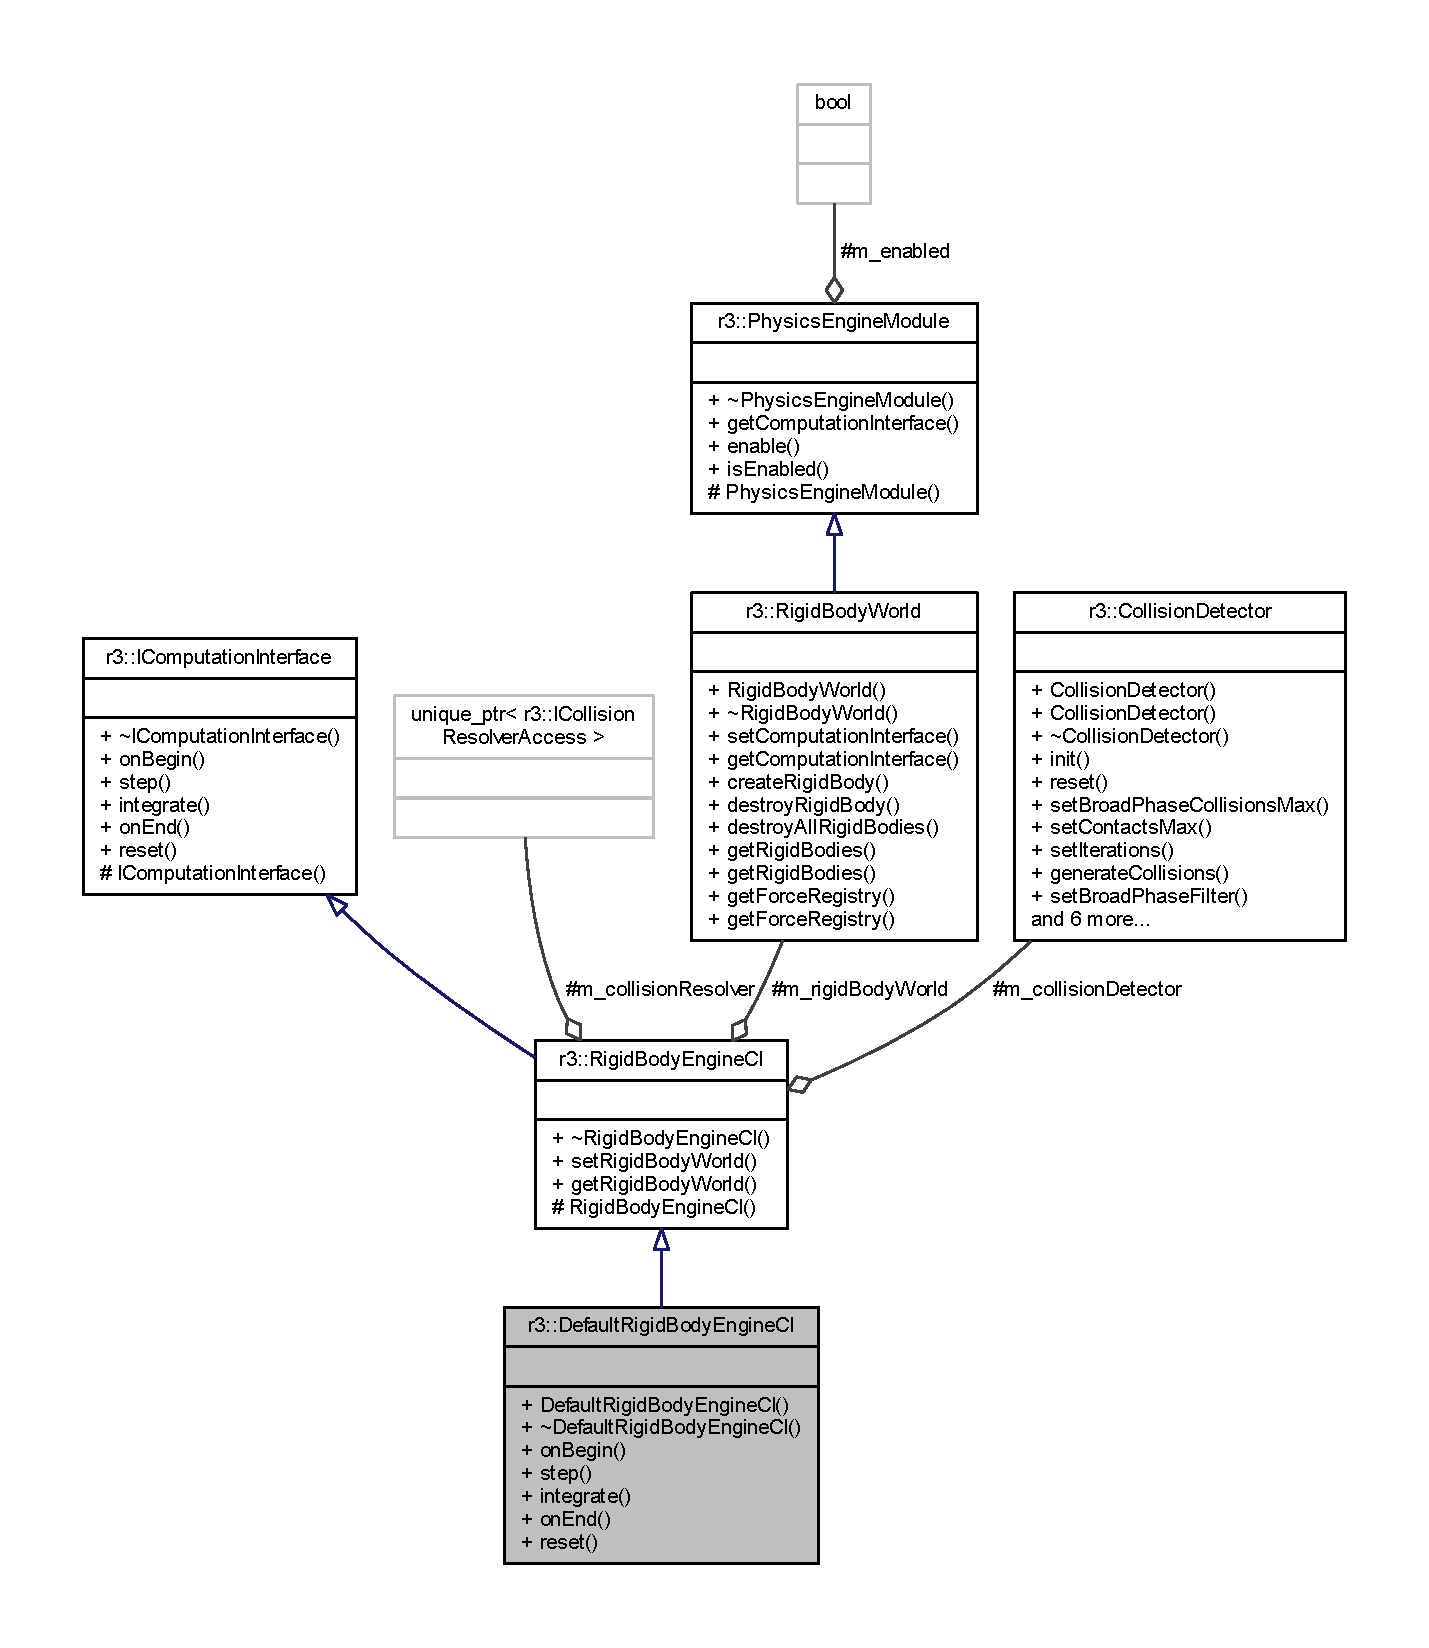
\includegraphics[width=350pt]{classr3_1_1_default_rigid_body_engine_c_i__coll__graph}
\end{center}
\end{figure}
\subsection*{Public Member Functions}
\begin{DoxyCompactItemize}
\item 
\mbox{\hyperlink{classr3_1_1_default_rigid_body_engine_c_i_a277f7da049340a3957fdaf8cb7ee0dfe}{Default\+Rigid\+Body\+Engine\+CI}} ()
\item 
\mbox{\hyperlink{classr3_1_1_default_rigid_body_engine_c_i_af68e19bbae7b792bf57d24a4004295eb}{$\sim$\+Default\+Rigid\+Body\+Engine\+CI}} ()
\item 
void \mbox{\hyperlink{classr3_1_1_default_rigid_body_engine_c_i_a5d9e40ea40845499f01081d21cd9ff64}{on\+Begin}} () override
\begin{DoxyCompactList}\small\item\em Prepare rigid bodies. \end{DoxyCompactList}\item 
void \mbox{\hyperlink{classr3_1_1_default_rigid_body_engine_c_i_ac45ae1d1889c75e6839b865870cbf59c}{step}} (\mbox{\hyperlink{namespacer3_ab2016b3e3f743fb735afce242f0dc1eb}{real}} time\+Delta) override
\begin{DoxyCompactList}\small\item\em Update forces on rigid bodies. \end{DoxyCompactList}\item 
void \mbox{\hyperlink{classr3_1_1_default_rigid_body_engine_c_i_a4b79e7e4bc76eedcad7ef5c4777b9d33}{integrate}} (\mbox{\hyperlink{namespacer3_ab2016b3e3f743fb735afce242f0dc1eb}{real}} time\+Delta) override
\begin{DoxyCompactList}\small\item\em Update positions, rotations and resolve collisions. \end{DoxyCompactList}\item 
void \mbox{\hyperlink{classr3_1_1_default_rigid_body_engine_c_i_ad7746126ebd5aab4cfc352dd9facabb2}{on\+End}} () override
\begin{DoxyCompactList}\small\item\em Clear accumulators. \end{DoxyCompactList}\item 
void \mbox{\hyperlink{classr3_1_1_default_rigid_body_engine_c_i_a06bd27e94b26017e7960e01f6e884e33}{reset}} () override
\begin{DoxyCompactList}\small\item\em Reset the computation interface. \end{DoxyCompactList}\end{DoxyCompactItemize}
\subsection*{Additional Inherited Members}


\subsection{Detailed Description}
Default implementation of the rigid body engine computation interface. 

\subsection{Constructor \& Destructor Documentation}
\mbox{\Hypertarget{classr3_1_1_default_rigid_body_engine_c_i_a277f7da049340a3957fdaf8cb7ee0dfe}\label{classr3_1_1_default_rigid_body_engine_c_i_a277f7da049340a3957fdaf8cb7ee0dfe}} 
\index{r3\+::\+Default\+Rigid\+Body\+Engine\+CI@{r3\+::\+Default\+Rigid\+Body\+Engine\+CI}!Default\+Rigid\+Body\+Engine\+CI@{Default\+Rigid\+Body\+Engine\+CI}}
\index{Default\+Rigid\+Body\+Engine\+CI@{Default\+Rigid\+Body\+Engine\+CI}!r3\+::\+Default\+Rigid\+Body\+Engine\+CI@{r3\+::\+Default\+Rigid\+Body\+Engine\+CI}}
\subsubsection{\texorpdfstring{Default\+Rigid\+Body\+Engine\+C\+I()}{DefaultRigidBodyEngineCI()}}
{\footnotesize\ttfamily r3\+::\+Default\+Rigid\+Body\+Engine\+C\+I\+::\+Default\+Rigid\+Body\+Engine\+CI (\begin{DoxyParamCaption}{ }\end{DoxyParamCaption})\hspace{0.3cm}{\ttfamily [explicit]}}

\mbox{\Hypertarget{classr3_1_1_default_rigid_body_engine_c_i_af68e19bbae7b792bf57d24a4004295eb}\label{classr3_1_1_default_rigid_body_engine_c_i_af68e19bbae7b792bf57d24a4004295eb}} 
\index{r3\+::\+Default\+Rigid\+Body\+Engine\+CI@{r3\+::\+Default\+Rigid\+Body\+Engine\+CI}!````~Default\+Rigid\+Body\+Engine\+CI@{$\sim$\+Default\+Rigid\+Body\+Engine\+CI}}
\index{````~Default\+Rigid\+Body\+Engine\+CI@{$\sim$\+Default\+Rigid\+Body\+Engine\+CI}!r3\+::\+Default\+Rigid\+Body\+Engine\+CI@{r3\+::\+Default\+Rigid\+Body\+Engine\+CI}}
\subsubsection{\texorpdfstring{$\sim$\+Default\+Rigid\+Body\+Engine\+C\+I()}{~DefaultRigidBodyEngineCI()}}
{\footnotesize\ttfamily r3\+::\+Default\+Rigid\+Body\+Engine\+C\+I\+::$\sim$\+Default\+Rigid\+Body\+Engine\+CI (\begin{DoxyParamCaption}{ }\end{DoxyParamCaption})\hspace{0.3cm}{\ttfamily [default]}}



\subsection{Member Function Documentation}
\mbox{\Hypertarget{classr3_1_1_default_rigid_body_engine_c_i_a4b79e7e4bc76eedcad7ef5c4777b9d33}\label{classr3_1_1_default_rigid_body_engine_c_i_a4b79e7e4bc76eedcad7ef5c4777b9d33}} 
\index{r3\+::\+Default\+Rigid\+Body\+Engine\+CI@{r3\+::\+Default\+Rigid\+Body\+Engine\+CI}!integrate@{integrate}}
\index{integrate@{integrate}!r3\+::\+Default\+Rigid\+Body\+Engine\+CI@{r3\+::\+Default\+Rigid\+Body\+Engine\+CI}}
\subsubsection{\texorpdfstring{integrate()}{integrate()}}
{\footnotesize\ttfamily void r3\+::\+Default\+Rigid\+Body\+Engine\+C\+I\+::integrate (\begin{DoxyParamCaption}\item[{\mbox{\hyperlink{namespacer3_ab2016b3e3f743fb735afce242f0dc1eb}{real}}}]{time\+Delta }\end{DoxyParamCaption})\hspace{0.3cm}{\ttfamily [override]}, {\ttfamily [virtual]}}



Update positions, rotations and resolve collisions. 


\begin{DoxyParams}{Parameters}
{\em time\+Delta} & Time step of the simulation update. \\
\hline
\end{DoxyParams}


Implements \mbox{\hyperlink{classr3_1_1_i_computation_interface_a162250f2b6efbd85460bd0f780d42cff}{r3\+::\+I\+Computation\+Interface}}.

\mbox{\Hypertarget{classr3_1_1_default_rigid_body_engine_c_i_a5d9e40ea40845499f01081d21cd9ff64}\label{classr3_1_1_default_rigid_body_engine_c_i_a5d9e40ea40845499f01081d21cd9ff64}} 
\index{r3\+::\+Default\+Rigid\+Body\+Engine\+CI@{r3\+::\+Default\+Rigid\+Body\+Engine\+CI}!on\+Begin@{on\+Begin}}
\index{on\+Begin@{on\+Begin}!r3\+::\+Default\+Rigid\+Body\+Engine\+CI@{r3\+::\+Default\+Rigid\+Body\+Engine\+CI}}
\subsubsection{\texorpdfstring{on\+Begin()}{onBegin()}}
{\footnotesize\ttfamily void r3\+::\+Default\+Rigid\+Body\+Engine\+C\+I\+::on\+Begin (\begin{DoxyParamCaption}{ }\end{DoxyParamCaption})\hspace{0.3cm}{\ttfamily [override]}, {\ttfamily [virtual]}}



Prepare rigid bodies. 



Implements \mbox{\hyperlink{classr3_1_1_i_computation_interface_a430ebc9cb8d4ba064ac6a032ef07edd7}{r3\+::\+I\+Computation\+Interface}}.

\mbox{\Hypertarget{classr3_1_1_default_rigid_body_engine_c_i_ad7746126ebd5aab4cfc352dd9facabb2}\label{classr3_1_1_default_rigid_body_engine_c_i_ad7746126ebd5aab4cfc352dd9facabb2}} 
\index{r3\+::\+Default\+Rigid\+Body\+Engine\+CI@{r3\+::\+Default\+Rigid\+Body\+Engine\+CI}!on\+End@{on\+End}}
\index{on\+End@{on\+End}!r3\+::\+Default\+Rigid\+Body\+Engine\+CI@{r3\+::\+Default\+Rigid\+Body\+Engine\+CI}}
\subsubsection{\texorpdfstring{on\+End()}{onEnd()}}
{\footnotesize\ttfamily void r3\+::\+Default\+Rigid\+Body\+Engine\+C\+I\+::on\+End (\begin{DoxyParamCaption}{ }\end{DoxyParamCaption})\hspace{0.3cm}{\ttfamily [override]}, {\ttfamily [virtual]}}



Clear accumulators. 



Implements \mbox{\hyperlink{classr3_1_1_i_computation_interface_acae0c5fada7e414c74fe6f5a8f4a6c7d}{r3\+::\+I\+Computation\+Interface}}.

\mbox{\Hypertarget{classr3_1_1_default_rigid_body_engine_c_i_a06bd27e94b26017e7960e01f6e884e33}\label{classr3_1_1_default_rigid_body_engine_c_i_a06bd27e94b26017e7960e01f6e884e33}} 
\index{r3\+::\+Default\+Rigid\+Body\+Engine\+CI@{r3\+::\+Default\+Rigid\+Body\+Engine\+CI}!reset@{reset}}
\index{reset@{reset}!r3\+::\+Default\+Rigid\+Body\+Engine\+CI@{r3\+::\+Default\+Rigid\+Body\+Engine\+CI}}
\subsubsection{\texorpdfstring{reset()}{reset()}}
{\footnotesize\ttfamily void r3\+::\+Default\+Rigid\+Body\+Engine\+C\+I\+::reset (\begin{DoxyParamCaption}{ }\end{DoxyParamCaption})\hspace{0.3cm}{\ttfamily [override]}, {\ttfamily [virtual]}}



Reset the computation interface. 



Implements \mbox{\hyperlink{classr3_1_1_i_computation_interface_a6069989c54ffd4e714788d0968851007}{r3\+::\+I\+Computation\+Interface}}.

\mbox{\Hypertarget{classr3_1_1_default_rigid_body_engine_c_i_ac45ae1d1889c75e6839b865870cbf59c}\label{classr3_1_1_default_rigid_body_engine_c_i_ac45ae1d1889c75e6839b865870cbf59c}} 
\index{r3\+::\+Default\+Rigid\+Body\+Engine\+CI@{r3\+::\+Default\+Rigid\+Body\+Engine\+CI}!step@{step}}
\index{step@{step}!r3\+::\+Default\+Rigid\+Body\+Engine\+CI@{r3\+::\+Default\+Rigid\+Body\+Engine\+CI}}
\subsubsection{\texorpdfstring{step()}{step()}}
{\footnotesize\ttfamily void r3\+::\+Default\+Rigid\+Body\+Engine\+C\+I\+::step (\begin{DoxyParamCaption}\item[{\mbox{\hyperlink{namespacer3_ab2016b3e3f743fb735afce242f0dc1eb}{real}}}]{time\+Delta }\end{DoxyParamCaption})\hspace{0.3cm}{\ttfamily [override]}, {\ttfamily [virtual]}}



Update forces on rigid bodies. 


\begin{DoxyParams}{Parameters}
{\em time\+Delta} & Time step of the simulation update. \\
\hline
\end{DoxyParams}


Implements \mbox{\hyperlink{classr3_1_1_i_computation_interface_aaa12bcc35005f32a1984b38de97696cb}{r3\+::\+I\+Computation\+Interface}}.



The documentation for this class was generated from the following files\+:\begin{DoxyCompactItemize}
\item 
C\+:/\+Library/\+Job/\+Projekte/\+Simulation\+Visualization/\+Rumble3\+D/\+Rumble3\+D/include/\+R3\+D/\+Rigid\+Body\+Engine/\mbox{\hyperlink{_default_rigid_body_engine_c_i_8h}{Default\+Rigid\+Body\+Engine\+C\+I.\+h}}\item 
C\+:/\+Library/\+Job/\+Projekte/\+Simulation\+Visualization/\+Rumble3\+D/\+Rumble3\+D/src/\+Rigid\+Body\+Engine/\mbox{\hyperlink{_default_rigid_body_engine_c_i_8cpp}{Default\+Rigid\+Body\+Engine\+C\+I.\+cpp}}\end{DoxyCompactItemize}

\hypertarget{classr3_1_1_directed_force}{}\section{r3\+:\+:Directed\+Force Class Reference}
\label{classr3_1_1_directed_force}\index{r3\+::\+Directed\+Force@{r3\+::\+Directed\+Force}}


A \mbox{\hyperlink{classr3_1_1_directed_force}{Directed\+Force}} is a force generator, which will continually apply a specified force at a specific body point.  




{\ttfamily \#include $<$Directed\+Force.\+h$>$}



Inheritance diagram for r3\+:\+:Directed\+Force\+:\nopagebreak
\begin{figure}[H]
\begin{center}
\leavevmode
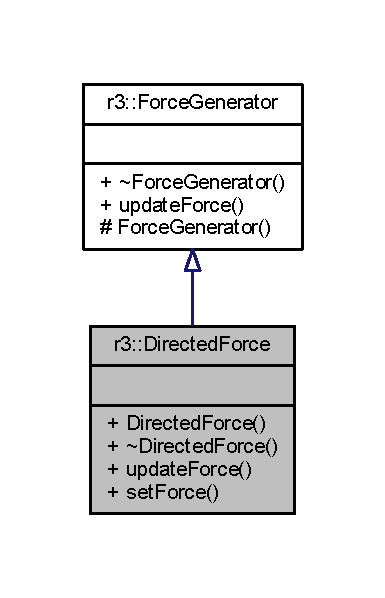
\includegraphics[width=185pt]{classr3_1_1_directed_force__inherit__graph}
\end{center}
\end{figure}


Collaboration diagram for r3\+:\+:Directed\+Force\+:\nopagebreak
\begin{figure}[H]
\begin{center}
\leavevmode
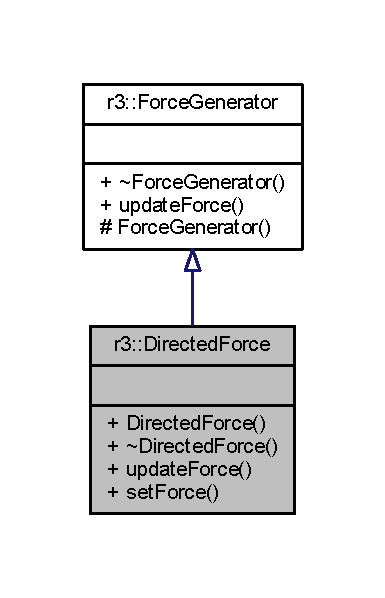
\includegraphics[width=185pt]{classr3_1_1_directed_force__coll__graph}
\end{center}
\end{figure}
\subsection*{Public Member Functions}
\begin{DoxyCompactItemize}
\item 
\mbox{\hyperlink{classr3_1_1_directed_force_a01b61a6ebe0c54f92952d69e3d0cf09e}{Directed\+Force}} (const glm\+::vec3 \&local\+Position, const glm\+::vec3 \&force)
\begin{DoxyCompactList}\small\item\em \mbox{\hyperlink{classr3_1_1_directed_force}{Directed\+Force}} constructor. \end{DoxyCompactList}\item 
\mbox{\hyperlink{classr3_1_1_directed_force_a98aa1b750a187ba18a6fce0c530e397f}{$\sim$\+Directed\+Force}} ()
\item 
void \mbox{\hyperlink{classr3_1_1_directed_force_ac723ddeef767956d16fb9d0a1d706bfd}{update\+Force}} (\mbox{\hyperlink{classr3_1_1_rigid_body}{Rigid\+Body}} $\ast$body, \mbox{\hyperlink{namespacer3_ab2016b3e3f743fb735afce242f0dc1eb}{real}} duration) override
\begin{DoxyCompactList}\small\item\em Apply force to a rigid body over a specific time. \end{DoxyCompactList}\item 
void \mbox{\hyperlink{classr3_1_1_directed_force_a5c25cdaa94e053ffd2614472d2a04c7e}{set\+Force}} (const glm\+::vec3 \&force)
\begin{DoxyCompactList}\small\item\em Set the force, which will act on the body. \end{DoxyCompactList}\end{DoxyCompactItemize}
\subsection*{Additional Inherited Members}


\subsection{Detailed Description}
A \mbox{\hyperlink{classr3_1_1_directed_force}{Directed\+Force}} is a force generator, which will continually apply a specified force at a specific body point. 

\subsection{Constructor \& Destructor Documentation}
\mbox{\Hypertarget{classr3_1_1_directed_force_a01b61a6ebe0c54f92952d69e3d0cf09e}\label{classr3_1_1_directed_force_a01b61a6ebe0c54f92952d69e3d0cf09e}} 
\index{r3\+::\+Directed\+Force@{r3\+::\+Directed\+Force}!Directed\+Force@{Directed\+Force}}
\index{Directed\+Force@{Directed\+Force}!r3\+::\+Directed\+Force@{r3\+::\+Directed\+Force}}
\subsubsection{\texorpdfstring{Directed\+Force()}{DirectedForce()}}
{\footnotesize\ttfamily r3\+::\+Directed\+Force\+::\+Directed\+Force (\begin{DoxyParamCaption}\item[{const glm\+::vec3 \&}]{local\+Position,  }\item[{const glm\+::vec3 \&}]{force }\end{DoxyParamCaption})}



\mbox{\hyperlink{classr3_1_1_directed_force}{Directed\+Force}} constructor. 


\begin{DoxyParams}{Parameters}
{\em local\+Position} & Attack point of the force. \\
\hline
{\em force} & The force, which will act on the body. \\
\hline
\end{DoxyParams}
\mbox{\Hypertarget{classr3_1_1_directed_force_a98aa1b750a187ba18a6fce0c530e397f}\label{classr3_1_1_directed_force_a98aa1b750a187ba18a6fce0c530e397f}} 
\index{r3\+::\+Directed\+Force@{r3\+::\+Directed\+Force}!````~Directed\+Force@{$\sim$\+Directed\+Force}}
\index{````~Directed\+Force@{$\sim$\+Directed\+Force}!r3\+::\+Directed\+Force@{r3\+::\+Directed\+Force}}
\subsubsection{\texorpdfstring{$\sim$\+Directed\+Force()}{~DirectedForce()}}
{\footnotesize\ttfamily r3\+::\+Directed\+Force\+::$\sim$\+Directed\+Force (\begin{DoxyParamCaption}{ }\end{DoxyParamCaption})\hspace{0.3cm}{\ttfamily [default]}}



\subsection{Member Function Documentation}
\mbox{\Hypertarget{classr3_1_1_directed_force_a5c25cdaa94e053ffd2614472d2a04c7e}\label{classr3_1_1_directed_force_a5c25cdaa94e053ffd2614472d2a04c7e}} 
\index{r3\+::\+Directed\+Force@{r3\+::\+Directed\+Force}!set\+Force@{set\+Force}}
\index{set\+Force@{set\+Force}!r3\+::\+Directed\+Force@{r3\+::\+Directed\+Force}}
\subsubsection{\texorpdfstring{set\+Force()}{setForce()}}
{\footnotesize\ttfamily void r3\+::\+Directed\+Force\+::set\+Force (\begin{DoxyParamCaption}\item[{const glm\+::vec3 \&}]{force }\end{DoxyParamCaption})}



Set the force, which will act on the body. 


\begin{DoxyParams}{Parameters}
{\em force} & The new force. \\
\hline
\end{DoxyParams}
\mbox{\Hypertarget{classr3_1_1_directed_force_ac723ddeef767956d16fb9d0a1d706bfd}\label{classr3_1_1_directed_force_ac723ddeef767956d16fb9d0a1d706bfd}} 
\index{r3\+::\+Directed\+Force@{r3\+::\+Directed\+Force}!update\+Force@{update\+Force}}
\index{update\+Force@{update\+Force}!r3\+::\+Directed\+Force@{r3\+::\+Directed\+Force}}
\subsubsection{\texorpdfstring{update\+Force()}{updateForce()}}
{\footnotesize\ttfamily void r3\+::\+Directed\+Force\+::update\+Force (\begin{DoxyParamCaption}\item[{\mbox{\hyperlink{classr3_1_1_rigid_body}{Rigid\+Body}} $\ast$}]{body,  }\item[{\mbox{\hyperlink{namespacer3_ab2016b3e3f743fb735afce242f0dc1eb}{real}}}]{duration }\end{DoxyParamCaption})\hspace{0.3cm}{\ttfamily [override]}, {\ttfamily [virtual]}}



Apply force to a rigid body over a specific time. 


\begin{DoxyParams}{Parameters}
{\em body} & The rigid body on which to apply force. \\
\hline
{\em duration} & The duration over which the force acts. \\
\hline
\end{DoxyParams}


Implements \mbox{\hyperlink{classr3_1_1_force_generator_a69bebbde8cef792d6636af50037af2aa}{r3\+::\+Force\+Generator}}.



The documentation for this class was generated from the following files\+:\begin{DoxyCompactItemize}
\item 
D\+:/\+Job/\+Forschungsmaster/\+Projekte/\+Simulation\+Visualization/\+Rumble3\+D/\+Rumble3\+D/include/\+R3\+D/\+Rigid\+Body\+Engine/\mbox{\hyperlink{_directed_force_8h}{Directed\+Force.\+h}}\item 
D\+:/\+Job/\+Forschungsmaster/\+Projekte/\+Simulation\+Visualization/\+Rumble3\+D/\+Rumble3\+D/src/\+Rigid\+Body\+Engine/\mbox{\hyperlink{_directed_force_8cpp}{Directed\+Force.\+cpp}}\end{DoxyCompactItemize}

\hypertarget{classr3_1_1_force_generator}{}\section{r3\+:\+:Force\+Generator Class Reference}
\label{classr3_1_1_force_generator}\index{r3\+::\+Force\+Generator@{r3\+::\+Force\+Generator}}


Interface for rigid body force generators.  




{\ttfamily \#include $<$Force\+Generator.\+h$>$}



Inheritance diagram for r3\+:\+:Force\+Generator\+:\nopagebreak
\begin{figure}[H]
\begin{center}
\leavevmode
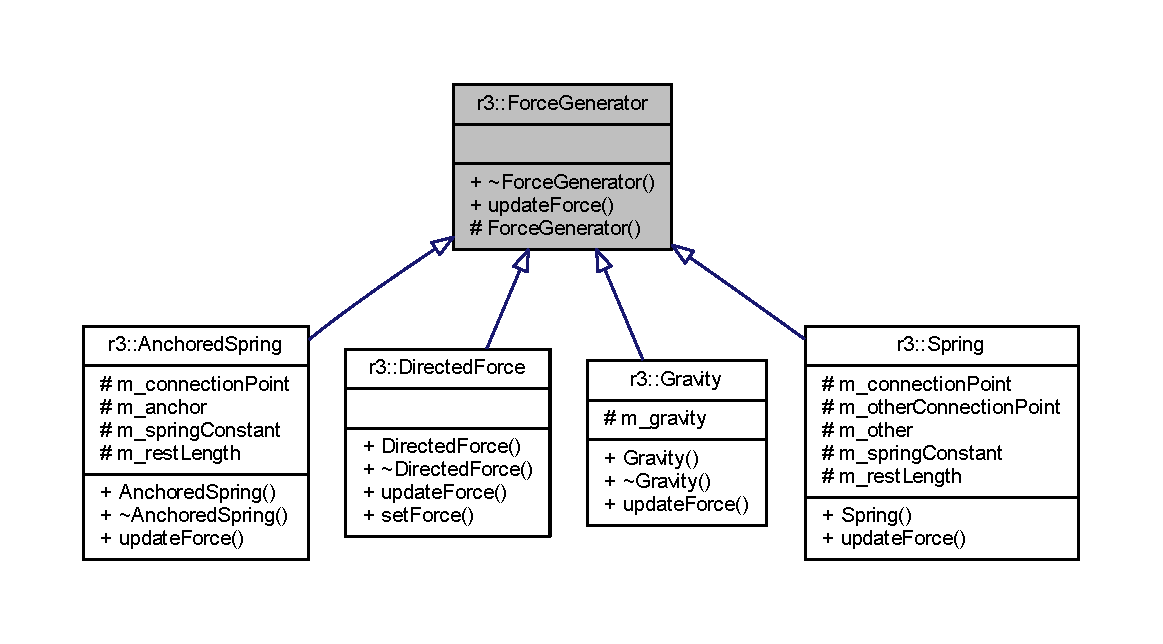
\includegraphics[width=350pt]{classr3_1_1_force_generator__inherit__graph}
\end{center}
\end{figure}


Collaboration diagram for r3\+:\+:Force\+Generator\+:\nopagebreak
\begin{figure}[H]
\begin{center}
\leavevmode
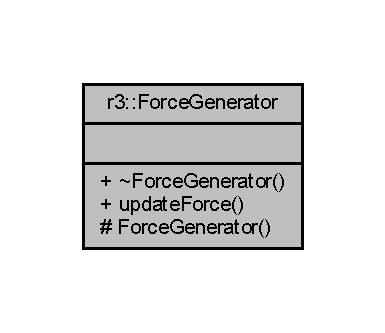
\includegraphics[width=185pt]{classr3_1_1_force_generator__coll__graph}
\end{center}
\end{figure}
\subsection*{Public Member Functions}
\begin{DoxyCompactItemize}
\item 
virtual \mbox{\hyperlink{classr3_1_1_force_generator_a64f1659bd0cf863ea28cccc689b2be3e}{$\sim$\+Force\+Generator}} ()
\item 
virtual void \mbox{\hyperlink{classr3_1_1_force_generator_a69bebbde8cef792d6636af50037af2aa}{update\+Force}} (\mbox{\hyperlink{classr3_1_1_rigid_body}{Rigid\+Body}} $\ast$body, \mbox{\hyperlink{namespacer3_ab2016b3e3f743fb735afce242f0dc1eb}{real}} duration)=0
\begin{DoxyCompactList}\small\item\em Apply force to a rigid body over a specific time. \end{DoxyCompactList}\end{DoxyCompactItemize}
\subsection*{Protected Member Functions}
\begin{DoxyCompactItemize}
\item 
\mbox{\hyperlink{classr3_1_1_force_generator_a7b21e48ccca59631975e0621057a1035}{Force\+Generator}} ()
\end{DoxyCompactItemize}


\subsection{Detailed Description}
Interface for rigid body force generators. 

\subsection{Constructor \& Destructor Documentation}
\mbox{\Hypertarget{classr3_1_1_force_generator_a64f1659bd0cf863ea28cccc689b2be3e}\label{classr3_1_1_force_generator_a64f1659bd0cf863ea28cccc689b2be3e}} 
\index{r3\+::\+Force\+Generator@{r3\+::\+Force\+Generator}!````~Force\+Generator@{$\sim$\+Force\+Generator}}
\index{````~Force\+Generator@{$\sim$\+Force\+Generator}!r3\+::\+Force\+Generator@{r3\+::\+Force\+Generator}}
\subsubsection{\texorpdfstring{$\sim$\+Force\+Generator()}{~ForceGenerator()}}
{\footnotesize\ttfamily r3\+::\+Force\+Generator\+::$\sim$\+Force\+Generator (\begin{DoxyParamCaption}{ }\end{DoxyParamCaption})\hspace{0.3cm}{\ttfamily [virtual]}, {\ttfamily [default]}}

\mbox{\Hypertarget{classr3_1_1_force_generator_a7b21e48ccca59631975e0621057a1035}\label{classr3_1_1_force_generator_a7b21e48ccca59631975e0621057a1035}} 
\index{r3\+::\+Force\+Generator@{r3\+::\+Force\+Generator}!Force\+Generator@{Force\+Generator}}
\index{Force\+Generator@{Force\+Generator}!r3\+::\+Force\+Generator@{r3\+::\+Force\+Generator}}
\subsubsection{\texorpdfstring{Force\+Generator()}{ForceGenerator()}}
{\footnotesize\ttfamily r3\+::\+Force\+Generator\+::\+Force\+Generator (\begin{DoxyParamCaption}{ }\end{DoxyParamCaption})\hspace{0.3cm}{\ttfamily [explicit]}, {\ttfamily [protected]}, {\ttfamily [default]}}



\subsection{Member Function Documentation}
\mbox{\Hypertarget{classr3_1_1_force_generator_a69bebbde8cef792d6636af50037af2aa}\label{classr3_1_1_force_generator_a69bebbde8cef792d6636af50037af2aa}} 
\index{r3\+::\+Force\+Generator@{r3\+::\+Force\+Generator}!update\+Force@{update\+Force}}
\index{update\+Force@{update\+Force}!r3\+::\+Force\+Generator@{r3\+::\+Force\+Generator}}
\subsubsection{\texorpdfstring{update\+Force()}{updateForce()}}
{\footnotesize\ttfamily virtual void r3\+::\+Force\+Generator\+::update\+Force (\begin{DoxyParamCaption}\item[{\mbox{\hyperlink{classr3_1_1_rigid_body}{Rigid\+Body}} $\ast$}]{body,  }\item[{\mbox{\hyperlink{namespacer3_ab2016b3e3f743fb735afce242f0dc1eb}{real}}}]{duration }\end{DoxyParamCaption})\hspace{0.3cm}{\ttfamily [pure virtual]}}



Apply force to a rigid body over a specific time. 


\begin{DoxyParams}{Parameters}
{\em body} & The rigid body on which to apply force. \\
\hline
{\em duration} & The duration over which the force acts. \\
\hline
\end{DoxyParams}


Implemented in \mbox{\hyperlink{classr3_1_1_spring_a3305adfd568606ed9ae6fb589f20446b}{r3\+::\+Spring}}, \mbox{\hyperlink{classr3_1_1_anchored_spring_a3e928bc7fdedc8eb5b302a007200a58c}{r3\+::\+Anchored\+Spring}}, \mbox{\hyperlink{classr3_1_1_directed_force_ac723ddeef767956d16fb9d0a1d706bfd}{r3\+::\+Directed\+Force}}, and \mbox{\hyperlink{classr3_1_1_gravity_ae3152c6a922ffa193aee362e161cd4a9}{r3\+::\+Gravity}}.



The documentation for this class was generated from the following files\+:\begin{DoxyCompactItemize}
\item 
D\+:/\+Job/\+Forschungsmaster/\+Projekte/\+Simulation\+Visualization/\+Rumble3\+D/\+Rumble3\+D/include/\+R3\+D/\+Rigid\+Body\+Engine/\mbox{\hyperlink{_force_generator_8h}{Force\+Generator.\+h}}\item 
D\+:/\+Job/\+Forschungsmaster/\+Projekte/\+Simulation\+Visualization/\+Rumble3\+D/\+Rumble3\+D/src/\+Rigid\+Body\+Engine/\mbox{\hyperlink{_force_generator_8cpp}{Force\+Generator.\+cpp}}\end{DoxyCompactItemize}

\hypertarget{structr3_1_1_force_registry_1_1_force_registration_entry}{}\section{r3\+:\+:Force\+Registry\+:\+:Force\+Registration\+Entry Struct Reference}
\label{structr3_1_1_force_registry_1_1_force_registration_entry}\index{r3\+::\+Force\+Registry\+::\+Force\+Registration\+Entry@{r3\+::\+Force\+Registry\+::\+Force\+Registration\+Entry}}


{\ttfamily \#include $<$Force\+Registry.\+h$>$}



Collaboration diagram for r3\+:\+:Force\+Registry\+:\+:Force\+Registration\+Entry\+:\nopagebreak
\begin{figure}[H]
\begin{center}
\leavevmode
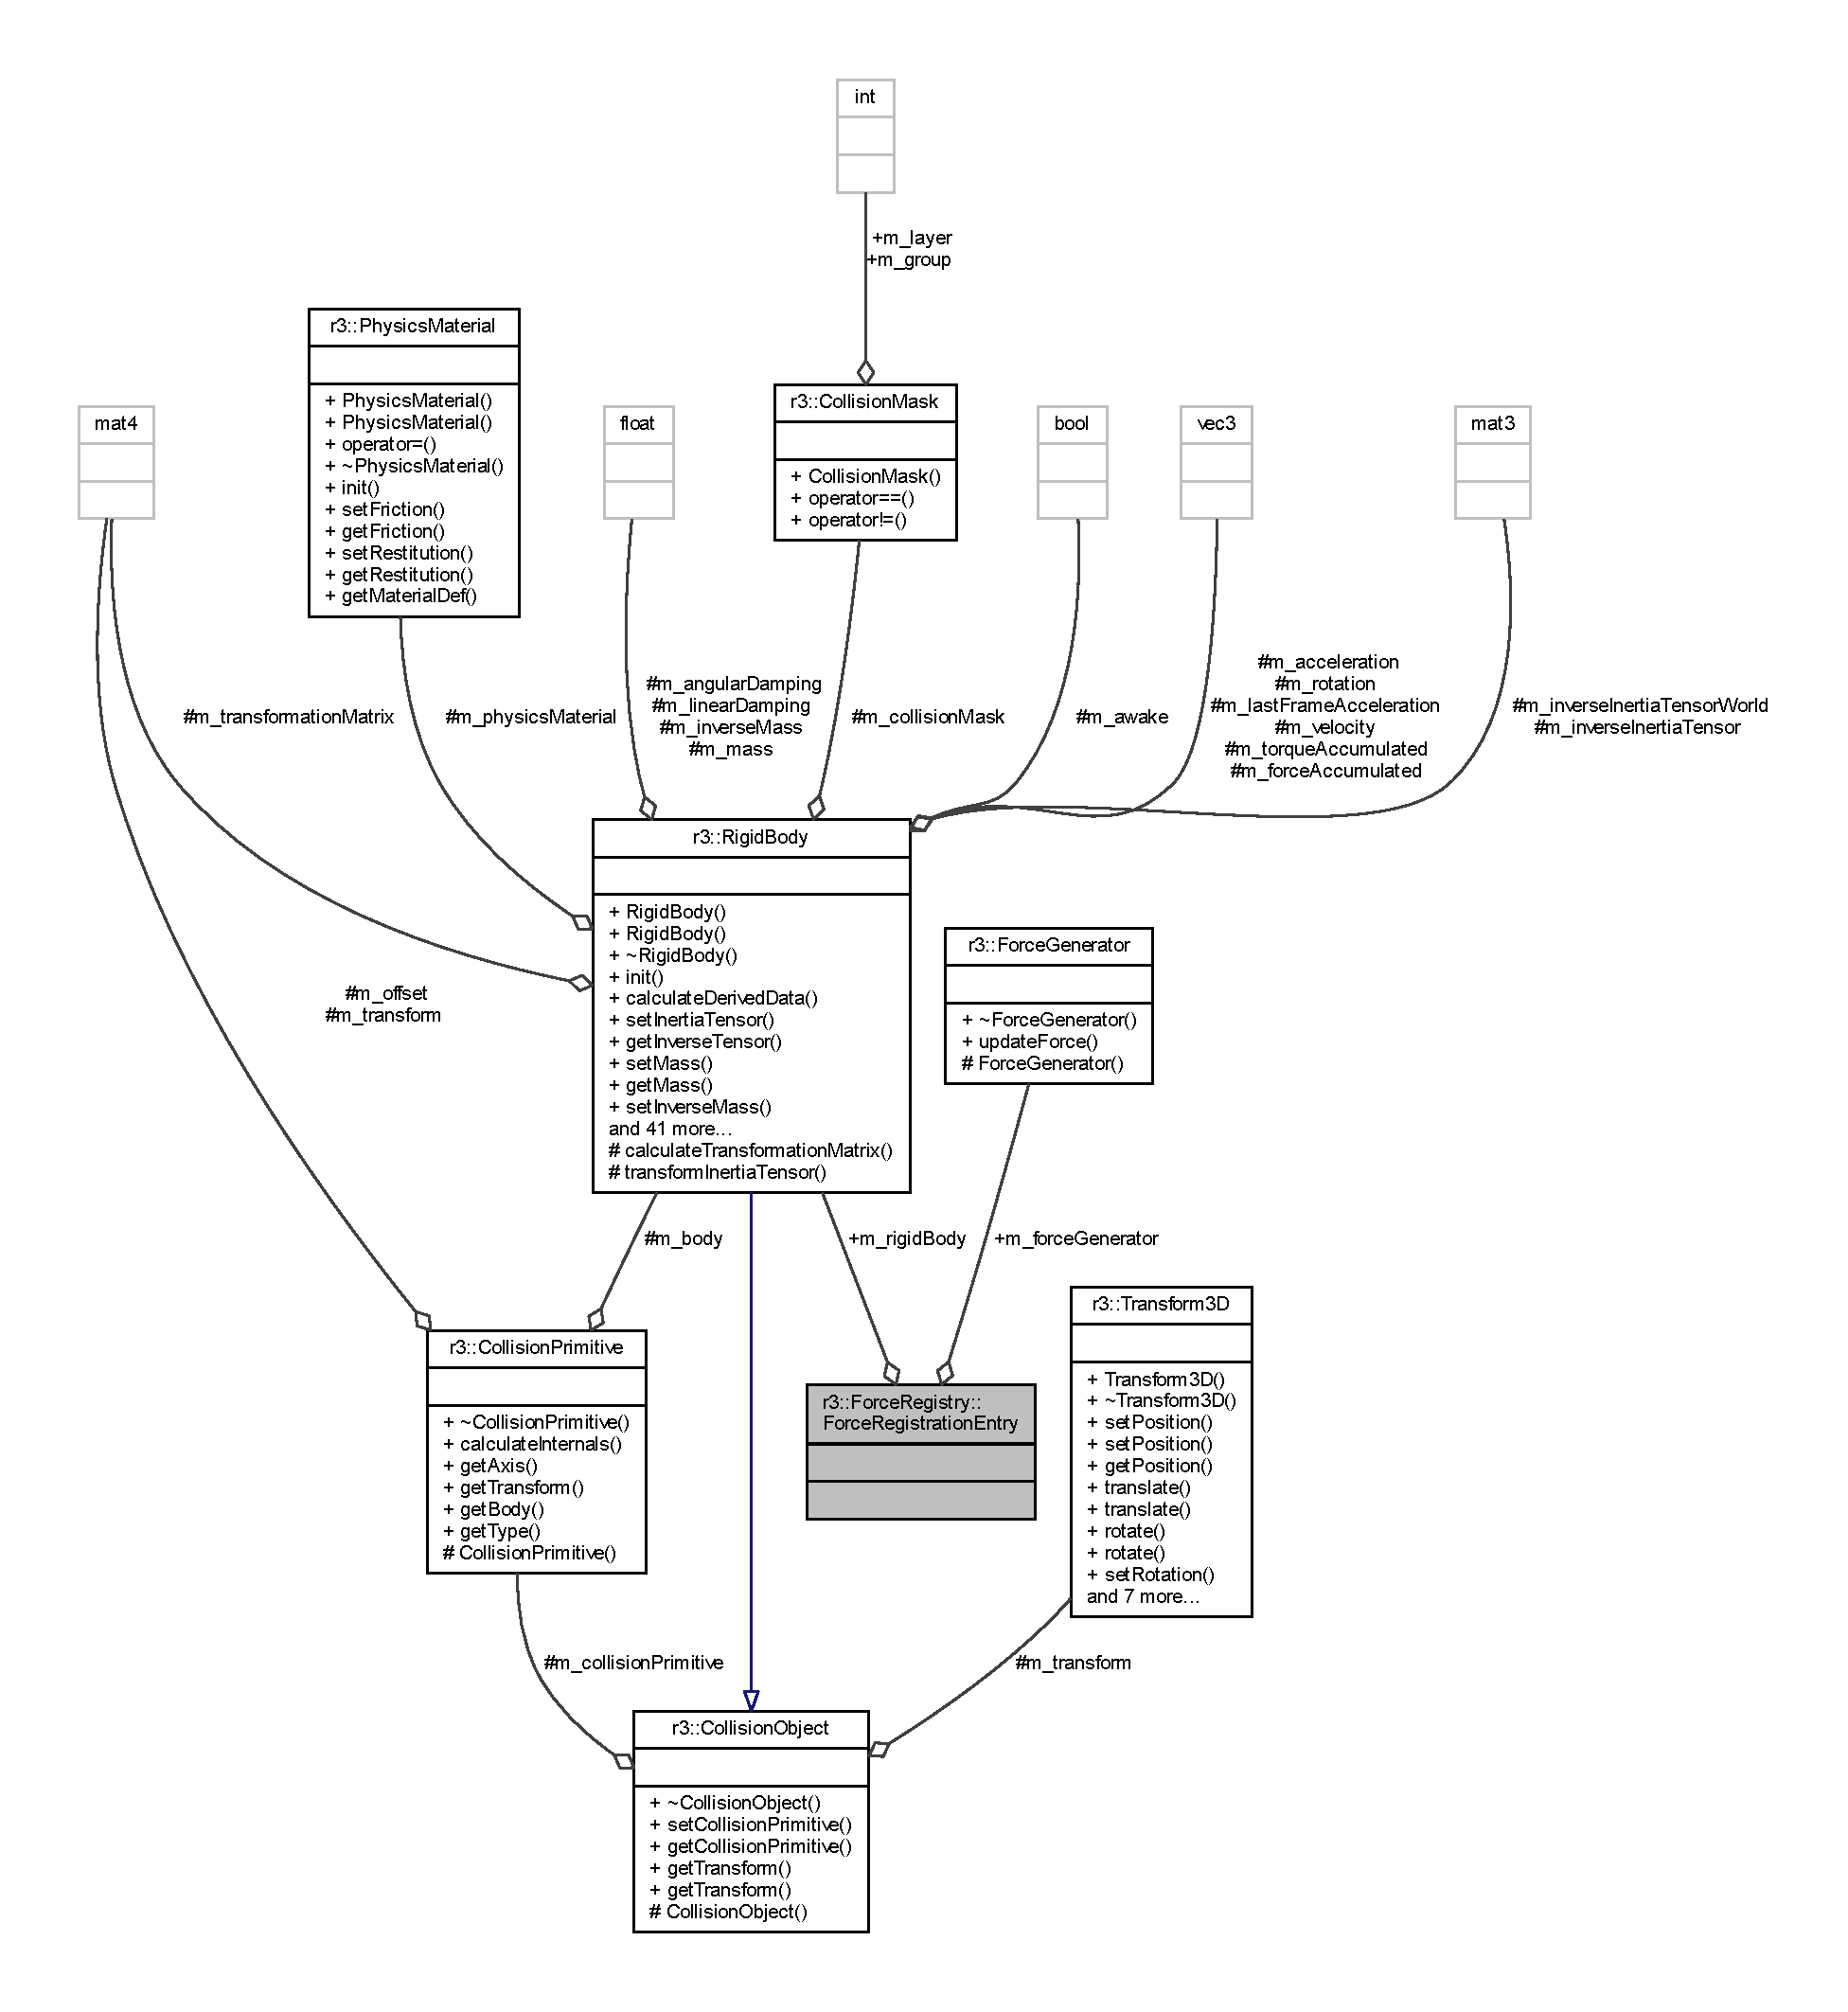
\includegraphics[width=350pt]{structr3_1_1_force_registry_1_1_force_registration_entry__coll__graph}
\end{center}
\end{figure}
\subsection*{Public Attributes}
\begin{DoxyCompactItemize}
\item 
\mbox{\hyperlink{classr3_1_1_rigid_body}{Rigid\+Body}} $\ast$ \mbox{\hyperlink{structr3_1_1_force_registry_1_1_force_registration_entry_a103ff58c0c8f46f2ed1927976bc5dc87}{m\+\_\+rigid\+Body}}
\item 
\mbox{\hyperlink{classr3_1_1_force_generator}{Force\+Generator}} $\ast$ \mbox{\hyperlink{structr3_1_1_force_registry_1_1_force_registration_entry_aa2af182d8c92d8da8d6045ea4f4a5e16}{m\+\_\+force\+Generator}}
\end{DoxyCompactItemize}


\subsection{Member Data Documentation}
\mbox{\Hypertarget{structr3_1_1_force_registry_1_1_force_registration_entry_aa2af182d8c92d8da8d6045ea4f4a5e16}\label{structr3_1_1_force_registry_1_1_force_registration_entry_aa2af182d8c92d8da8d6045ea4f4a5e16}} 
\index{r3\+::\+Force\+Registry\+::\+Force\+Registration\+Entry@{r3\+::\+Force\+Registry\+::\+Force\+Registration\+Entry}!m\+\_\+force\+Generator@{m\+\_\+force\+Generator}}
\index{m\+\_\+force\+Generator@{m\+\_\+force\+Generator}!r3\+::\+Force\+Registry\+::\+Force\+Registration\+Entry@{r3\+::\+Force\+Registry\+::\+Force\+Registration\+Entry}}
\subsubsection{\texorpdfstring{m\+\_\+force\+Generator}{m\_forceGenerator}}
{\footnotesize\ttfamily \mbox{\hyperlink{classr3_1_1_force_generator}{Force\+Generator}}$\ast$ r3\+::\+Force\+Registry\+::\+Force\+Registration\+Entry\+::m\+\_\+force\+Generator}

\mbox{\Hypertarget{structr3_1_1_force_registry_1_1_force_registration_entry_a103ff58c0c8f46f2ed1927976bc5dc87}\label{structr3_1_1_force_registry_1_1_force_registration_entry_a103ff58c0c8f46f2ed1927976bc5dc87}} 
\index{r3\+::\+Force\+Registry\+::\+Force\+Registration\+Entry@{r3\+::\+Force\+Registry\+::\+Force\+Registration\+Entry}!m\+\_\+rigid\+Body@{m\+\_\+rigid\+Body}}
\index{m\+\_\+rigid\+Body@{m\+\_\+rigid\+Body}!r3\+::\+Force\+Registry\+::\+Force\+Registration\+Entry@{r3\+::\+Force\+Registry\+::\+Force\+Registration\+Entry}}
\subsubsection{\texorpdfstring{m\+\_\+rigid\+Body}{m\_rigidBody}}
{\footnotesize\ttfamily \mbox{\hyperlink{classr3_1_1_rigid_body}{Rigid\+Body}}$\ast$ r3\+::\+Force\+Registry\+::\+Force\+Registration\+Entry\+::m\+\_\+rigid\+Body}



The documentation for this struct was generated from the following file\+:\begin{DoxyCompactItemize}
\item 
D\+:/\+Library/\+Documents/\+Job/\+Forschungsmaster/\+Projekte/\+Simulation\+Visualization/\+Rumble3\+D/\+Rumble3\+D/include/\+R3\+D/\+Rigid\+Body\+Engine/\mbox{\hyperlink{_force_registry_8h}{Force\+Registry.\+h}}\end{DoxyCompactItemize}

\hypertarget{classr3_1_1_force_registry}{}\section{r3\+:\+:Force\+Registry Class Reference}
\label{classr3_1_1_force_registry}\index{r3\+::\+Force\+Registry@{r3\+::\+Force\+Registry}}


{\ttfamily \#include $<$Force\+Registry.\+h$>$}



Collaboration diagram for r3\+:\+:Force\+Registry\+:\nopagebreak
\begin{figure}[H]
\begin{center}
\leavevmode
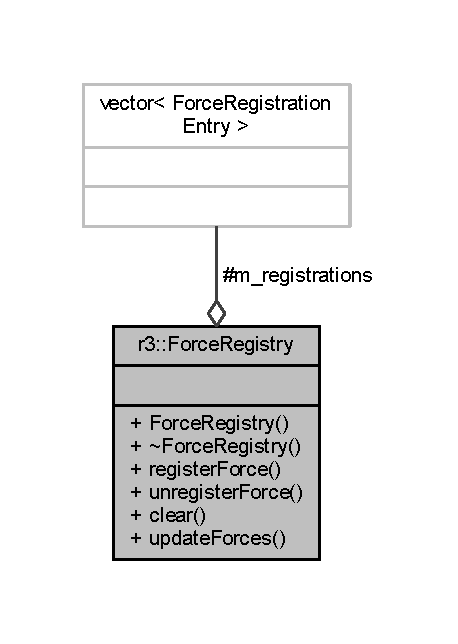
\includegraphics[width=220pt]{classr3_1_1_force_registry__coll__graph}
\end{center}
\end{figure}
\subsection*{Classes}
\begin{DoxyCompactItemize}
\item 
struct \mbox{\hyperlink{structr3_1_1_force_registry_1_1_force_registration_entry}{Force\+Registration\+Entry}}
\end{DoxyCompactItemize}
\subsection*{Public Types}
\begin{DoxyCompactItemize}
\item 
using \mbox{\hyperlink{classr3_1_1_force_registry_a91449a71b1a33d773ef787ae56ae9b2d}{Registry}} = std\+::vector$<$ \mbox{\hyperlink{structr3_1_1_force_registry_1_1_force_registration_entry}{Force\+Registration\+Entry}} $>$
\end{DoxyCompactItemize}
\subsection*{Public Member Functions}
\begin{DoxyCompactItemize}
\item 
\mbox{\hyperlink{classr3_1_1_force_registry_a6830132c53a756ebf3e6621195f51b17}{Force\+Registry}} ()
\item 
\mbox{\hyperlink{classr3_1_1_force_registry_a322cdf54468a6f59610562a7bfc2e60d}{$\sim$\+Force\+Registry}} ()
\item 
void \mbox{\hyperlink{classr3_1_1_force_registry_a2b86303ed6ac2082606b298301f9957c}{register\+Force}} (\mbox{\hyperlink{classr3_1_1_rigid_body}{Rigid\+Body}} $\ast$rigid\+Body, \mbox{\hyperlink{classr3_1_1_force_generator}{Force\+Generator}} $\ast$fg)
\item 
void \mbox{\hyperlink{classr3_1_1_force_registry_a3a6163fed4266bd6e18ebad2c5c939cd}{unregister\+Force}} (\mbox{\hyperlink{classr3_1_1_rigid_body}{Rigid\+Body}} $\ast$rigid\+Body, \mbox{\hyperlink{classr3_1_1_force_generator}{Force\+Generator}} $\ast$fg)
\item 
void \mbox{\hyperlink{classr3_1_1_force_registry_ab1c31bc403d998af16df97ff5d42c95f}{clear}} ()
\item 
void \mbox{\hyperlink{classr3_1_1_force_registry_a34d6ad7472e2f47dfd3416a703eca78e}{update\+Forces}} (\mbox{\hyperlink{namespacer3_ab2016b3e3f743fb735afce242f0dc1eb}{real}} duration)
\end{DoxyCompactItemize}
\subsection*{Protected Attributes}
\begin{DoxyCompactItemize}
\item 
\mbox{\hyperlink{classr3_1_1_force_registry_a91449a71b1a33d773ef787ae56ae9b2d}{Registry}} \mbox{\hyperlink{classr3_1_1_force_registry_a36847da26301dc4b18e6b6b25fb2fa51}{m\+\_\+registrations}}
\end{DoxyCompactItemize}


\subsection{Member Typedef Documentation}
\mbox{\Hypertarget{classr3_1_1_force_registry_a91449a71b1a33d773ef787ae56ae9b2d}\label{classr3_1_1_force_registry_a91449a71b1a33d773ef787ae56ae9b2d}} 
\index{r3\+::\+Force\+Registry@{r3\+::\+Force\+Registry}!Registry@{Registry}}
\index{Registry@{Registry}!r3\+::\+Force\+Registry@{r3\+::\+Force\+Registry}}
\subsubsection{\texorpdfstring{Registry}{Registry}}
{\footnotesize\ttfamily using \mbox{\hyperlink{classr3_1_1_force_registry_a91449a71b1a33d773ef787ae56ae9b2d}{r3\+::\+Force\+Registry\+::\+Registry}} =  std\+::vector$<$\mbox{\hyperlink{structr3_1_1_force_registry_1_1_force_registration_entry}{Force\+Registration\+Entry}}$>$}



\subsection{Constructor \& Destructor Documentation}
\mbox{\Hypertarget{classr3_1_1_force_registry_a6830132c53a756ebf3e6621195f51b17}\label{classr3_1_1_force_registry_a6830132c53a756ebf3e6621195f51b17}} 
\index{r3\+::\+Force\+Registry@{r3\+::\+Force\+Registry}!Force\+Registry@{Force\+Registry}}
\index{Force\+Registry@{Force\+Registry}!r3\+::\+Force\+Registry@{r3\+::\+Force\+Registry}}
\subsubsection{\texorpdfstring{Force\+Registry()}{ForceRegistry()}}
{\footnotesize\ttfamily r3\+::\+Force\+Registry\+::\+Force\+Registry (\begin{DoxyParamCaption}{ }\end{DoxyParamCaption})\hspace{0.3cm}{\ttfamily [explicit]}, {\ttfamily [default]}}

\mbox{\Hypertarget{classr3_1_1_force_registry_a322cdf54468a6f59610562a7bfc2e60d}\label{classr3_1_1_force_registry_a322cdf54468a6f59610562a7bfc2e60d}} 
\index{r3\+::\+Force\+Registry@{r3\+::\+Force\+Registry}!````~Force\+Registry@{$\sim$\+Force\+Registry}}
\index{````~Force\+Registry@{$\sim$\+Force\+Registry}!r3\+::\+Force\+Registry@{r3\+::\+Force\+Registry}}
\subsubsection{\texorpdfstring{$\sim$\+Force\+Registry()}{~ForceRegistry()}}
{\footnotesize\ttfamily r3\+::\+Force\+Registry\+::$\sim$\+Force\+Registry (\begin{DoxyParamCaption}{ }\end{DoxyParamCaption})\hspace{0.3cm}{\ttfamily [default]}}



\subsection{Member Function Documentation}
\mbox{\Hypertarget{classr3_1_1_force_registry_ab1c31bc403d998af16df97ff5d42c95f}\label{classr3_1_1_force_registry_ab1c31bc403d998af16df97ff5d42c95f}} 
\index{r3\+::\+Force\+Registry@{r3\+::\+Force\+Registry}!clear@{clear}}
\index{clear@{clear}!r3\+::\+Force\+Registry@{r3\+::\+Force\+Registry}}
\subsubsection{\texorpdfstring{clear()}{clear()}}
{\footnotesize\ttfamily void r3\+::\+Force\+Registry\+::clear (\begin{DoxyParamCaption}{ }\end{DoxyParamCaption})}

\mbox{\Hypertarget{classr3_1_1_force_registry_a2b86303ed6ac2082606b298301f9957c}\label{classr3_1_1_force_registry_a2b86303ed6ac2082606b298301f9957c}} 
\index{r3\+::\+Force\+Registry@{r3\+::\+Force\+Registry}!register\+Force@{register\+Force}}
\index{register\+Force@{register\+Force}!r3\+::\+Force\+Registry@{r3\+::\+Force\+Registry}}
\subsubsection{\texorpdfstring{register\+Force()}{registerForce()}}
{\footnotesize\ttfamily void r3\+::\+Force\+Registry\+::register\+Force (\begin{DoxyParamCaption}\item[{\mbox{\hyperlink{classr3_1_1_rigid_body}{Rigid\+Body}} $\ast$}]{rigid\+Body,  }\item[{\mbox{\hyperlink{classr3_1_1_force_generator}{Force\+Generator}} $\ast$}]{fg }\end{DoxyParamCaption})}

\mbox{\Hypertarget{classr3_1_1_force_registry_a3a6163fed4266bd6e18ebad2c5c939cd}\label{classr3_1_1_force_registry_a3a6163fed4266bd6e18ebad2c5c939cd}} 
\index{r3\+::\+Force\+Registry@{r3\+::\+Force\+Registry}!unregister\+Force@{unregister\+Force}}
\index{unregister\+Force@{unregister\+Force}!r3\+::\+Force\+Registry@{r3\+::\+Force\+Registry}}
\subsubsection{\texorpdfstring{unregister\+Force()}{unregisterForce()}}
{\footnotesize\ttfamily void r3\+::\+Force\+Registry\+::unregister\+Force (\begin{DoxyParamCaption}\item[{\mbox{\hyperlink{classr3_1_1_rigid_body}{Rigid\+Body}} $\ast$}]{rigid\+Body,  }\item[{\mbox{\hyperlink{classr3_1_1_force_generator}{Force\+Generator}} $\ast$}]{fg }\end{DoxyParamCaption})}

\mbox{\Hypertarget{classr3_1_1_force_registry_a34d6ad7472e2f47dfd3416a703eca78e}\label{classr3_1_1_force_registry_a34d6ad7472e2f47dfd3416a703eca78e}} 
\index{r3\+::\+Force\+Registry@{r3\+::\+Force\+Registry}!update\+Forces@{update\+Forces}}
\index{update\+Forces@{update\+Forces}!r3\+::\+Force\+Registry@{r3\+::\+Force\+Registry}}
\subsubsection{\texorpdfstring{update\+Forces()}{updateForces()}}
{\footnotesize\ttfamily void r3\+::\+Force\+Registry\+::update\+Forces (\begin{DoxyParamCaption}\item[{\mbox{\hyperlink{namespacer3_ab2016b3e3f743fb735afce242f0dc1eb}{real}}}]{duration }\end{DoxyParamCaption})}



\subsection{Member Data Documentation}
\mbox{\Hypertarget{classr3_1_1_force_registry_a36847da26301dc4b18e6b6b25fb2fa51}\label{classr3_1_1_force_registry_a36847da26301dc4b18e6b6b25fb2fa51}} 
\index{r3\+::\+Force\+Registry@{r3\+::\+Force\+Registry}!m\+\_\+registrations@{m\+\_\+registrations}}
\index{m\+\_\+registrations@{m\+\_\+registrations}!r3\+::\+Force\+Registry@{r3\+::\+Force\+Registry}}
\subsubsection{\texorpdfstring{m\+\_\+registrations}{m\_registrations}}
{\footnotesize\ttfamily \mbox{\hyperlink{classr3_1_1_force_registry_a91449a71b1a33d773ef787ae56ae9b2d}{Registry}} r3\+::\+Force\+Registry\+::m\+\_\+registrations\hspace{0.3cm}{\ttfamily [protected]}}



The documentation for this class was generated from the following files\+:\begin{DoxyCompactItemize}
\item 
D\+:/\+Job/\+Forschungsmaster/\+Projekte/\+Simulation\+Visualization/\+Rumble3\+D/\+Rumble3\+D/include/\+R3\+D/\+Rigid\+Body\+Engine/\mbox{\hyperlink{_force_registry_8h}{Force\+Registry.\+h}}\item 
D\+:/\+Job/\+Forschungsmaster/\+Projekte/\+Simulation\+Visualization/\+Rumble3\+D/\+Rumble3\+D/src/\+Rigid\+Body\+Engine/\mbox{\hyperlink{_force_registry_8cpp}{Force\+Registry.\+cpp}}\end{DoxyCompactItemize}

\hypertarget{classr3_1_1_friction_resolver}{}\section{r3\+:\+:Friction\+Resolver Class Reference}
\label{classr3_1_1_friction_resolver}\index{r3\+::\+Friction\+Resolver@{r3\+::\+Friction\+Resolver}}


{\ttfamily \#include $<$Friction\+Resolver.\+h$>$}



Inheritance diagram for r3\+:\+:Friction\+Resolver\+:\nopagebreak
\begin{figure}[H]
\begin{center}
\leavevmode
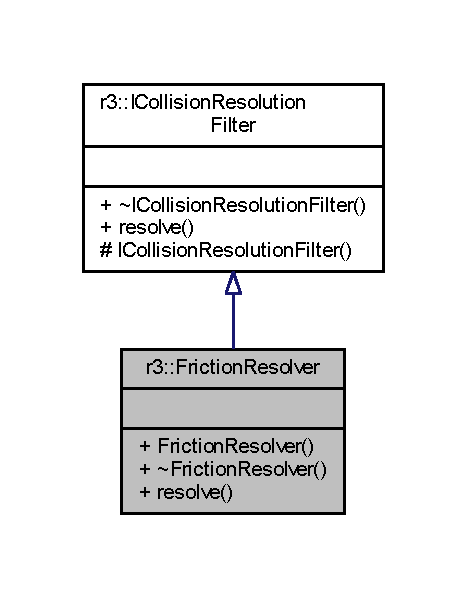
\includegraphics[width=224pt]{classr3_1_1_friction_resolver__inherit__graph}
\end{center}
\end{figure}


Collaboration diagram for r3\+:\+:Friction\+Resolver\+:\nopagebreak
\begin{figure}[H]
\begin{center}
\leavevmode
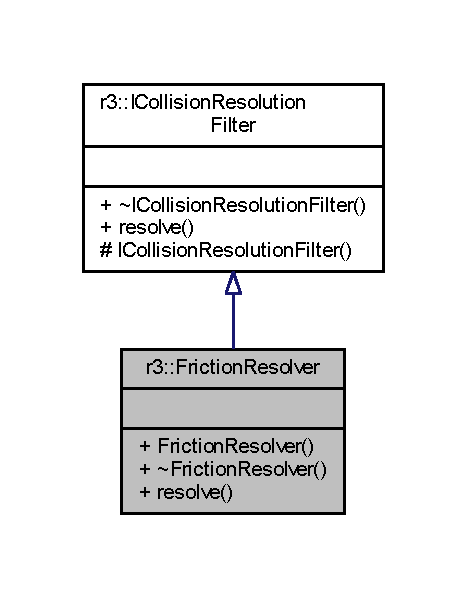
\includegraphics[width=224pt]{classr3_1_1_friction_resolver__coll__graph}
\end{center}
\end{figure}
\subsection*{Public Member Functions}
\begin{DoxyCompactItemize}
\item 
\mbox{\hyperlink{classr3_1_1_friction_resolver_a55a3a08603cf362da1896ec2ccc026ba}{Friction\+Resolver}} ()
\item 
\mbox{\hyperlink{classr3_1_1_friction_resolver_a49a41d6820e9c9c17447c79303296dea}{$\sim$\+Friction\+Resolver}} ()
\item 
void \mbox{\hyperlink{classr3_1_1_friction_resolver_aa6c4e02ba5ec9759eea10900cdcf44f5}{resolve}} (const \mbox{\hyperlink{classr3_1_1_collision_data}{Collision\+Data}} \&collision\+Data) override
\end{DoxyCompactItemize}
\subsection*{Additional Inherited Members}


\subsection{Constructor \& Destructor Documentation}
\mbox{\Hypertarget{classr3_1_1_friction_resolver_a55a3a08603cf362da1896ec2ccc026ba}\label{classr3_1_1_friction_resolver_a55a3a08603cf362da1896ec2ccc026ba}} 
\index{r3\+::\+Friction\+Resolver@{r3\+::\+Friction\+Resolver}!Friction\+Resolver@{Friction\+Resolver}}
\index{Friction\+Resolver@{Friction\+Resolver}!r3\+::\+Friction\+Resolver@{r3\+::\+Friction\+Resolver}}
\subsubsection{\texorpdfstring{Friction\+Resolver()}{FrictionResolver()}}
{\footnotesize\ttfamily r3\+::\+Friction\+Resolver\+::\+Friction\+Resolver (\begin{DoxyParamCaption}{ }\end{DoxyParamCaption})\hspace{0.3cm}{\ttfamily [explicit]}, {\ttfamily [default]}}

\mbox{\Hypertarget{classr3_1_1_friction_resolver_a49a41d6820e9c9c17447c79303296dea}\label{classr3_1_1_friction_resolver_a49a41d6820e9c9c17447c79303296dea}} 
\index{r3\+::\+Friction\+Resolver@{r3\+::\+Friction\+Resolver}!````~Friction\+Resolver@{$\sim$\+Friction\+Resolver}}
\index{````~Friction\+Resolver@{$\sim$\+Friction\+Resolver}!r3\+::\+Friction\+Resolver@{r3\+::\+Friction\+Resolver}}
\subsubsection{\texorpdfstring{$\sim$\+Friction\+Resolver()}{~FrictionResolver()}}
{\footnotesize\ttfamily r3\+::\+Friction\+Resolver\+::$\sim$\+Friction\+Resolver (\begin{DoxyParamCaption}{ }\end{DoxyParamCaption})\hspace{0.3cm}{\ttfamily [default]}}



\subsection{Member Function Documentation}
\mbox{\Hypertarget{classr3_1_1_friction_resolver_aa6c4e02ba5ec9759eea10900cdcf44f5}\label{classr3_1_1_friction_resolver_aa6c4e02ba5ec9759eea10900cdcf44f5}} 
\index{r3\+::\+Friction\+Resolver@{r3\+::\+Friction\+Resolver}!resolve@{resolve}}
\index{resolve@{resolve}!r3\+::\+Friction\+Resolver@{r3\+::\+Friction\+Resolver}}
\subsubsection{\texorpdfstring{resolve()}{resolve()}}
{\footnotesize\ttfamily void r3\+::\+Friction\+Resolver\+::resolve (\begin{DoxyParamCaption}\item[{const \mbox{\hyperlink{classr3_1_1_collision_data}{Collision\+Data}} \&}]{collision\+Data }\end{DoxyParamCaption})\hspace{0.3cm}{\ttfamily [override]}, {\ttfamily [virtual]}}



Implements \mbox{\hyperlink{classr3_1_1_i_collision_resolution_filter_a9ae35c07c585500c409459ef87e5ae15}{r3\+::\+I\+Collision\+Resolution\+Filter}}.



The documentation for this class was generated from the following files\+:\begin{DoxyCompactItemize}
\item 
D\+:/\+Library/\+Documents/\+Job/\+Forschungsmaster/\+Projekte/\+Simulation\+Visualization/\+Rumble3\+D/\+Rumble3\+D/include/\+R3\+D/\+Rigid\+Body\+Engine/\+Collision\+Resolution/\mbox{\hyperlink{_friction_resolver_8h}{Friction\+Resolver.\+h}}\item 
D\+:/\+Library/\+Documents/\+Job/\+Forschungsmaster/\+Projekte/\+Simulation\+Visualization/\+Rumble3\+D/\+Rumble3\+D/src/\+Rigid\+Body\+Engine/\+Collision\+Resolution/\mbox{\hyperlink{_friction_resolver_8cpp}{Friction\+Resolver.\+cpp}}\end{DoxyCompactItemize}

\hypertarget{classr3_1_1_gravity}{}\section{r3\+:\+:Gravity Class Reference}
\label{classr3_1_1_gravity}\index{r3\+::\+Gravity@{r3\+::\+Gravity}}


\mbox{\hyperlink{classr3_1_1_gravity}{Gravity}} is a force generator, which will apply constant force on bodies.  




{\ttfamily \#include $<$Gravity.\+h$>$}



Inheritance diagram for r3\+:\+:Gravity\+:\nopagebreak
\begin{figure}[H]
\begin{center}
\leavevmode
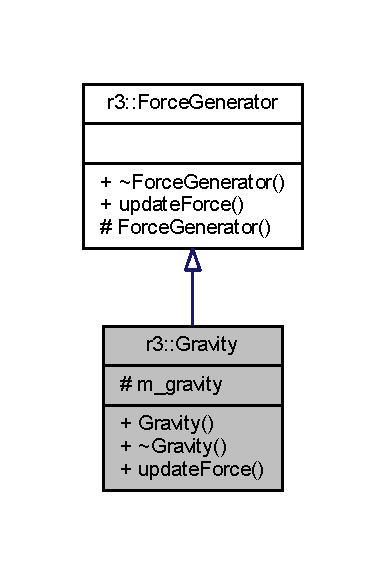
\includegraphics[width=185pt]{classr3_1_1_gravity__inherit__graph}
\end{center}
\end{figure}


Collaboration diagram for r3\+:\+:Gravity\+:\nopagebreak
\begin{figure}[H]
\begin{center}
\leavevmode
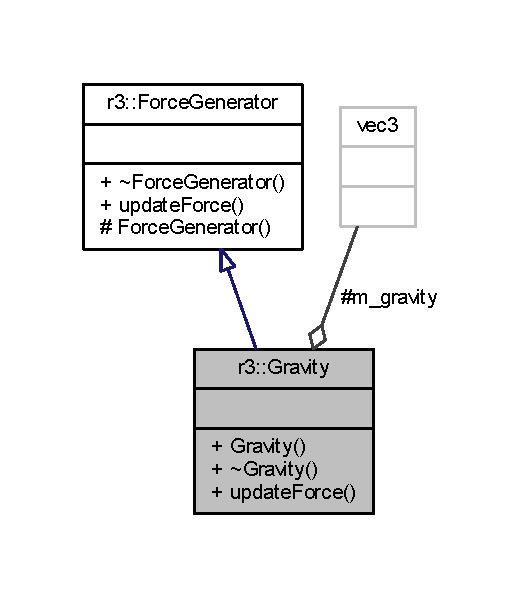
\includegraphics[width=251pt]{classr3_1_1_gravity__coll__graph}
\end{center}
\end{figure}
\subsection*{Public Member Functions}
\begin{DoxyCompactItemize}
\item 
\mbox{\hyperlink{classr3_1_1_gravity_a1c5f6d085a7b1484c23f5a6df4b58b05}{Gravity}} (const glm\+::vec3 \&gravity)
\begin{DoxyCompactList}\small\item\em \mbox{\hyperlink{classr3_1_1_gravity}{Gravity}} constructor. \end{DoxyCompactList}\item 
\mbox{\hyperlink{classr3_1_1_gravity_abdf3edf32d08b6c5b9c2fc161635f993}{$\sim$\+Gravity}} ()
\item 
void \mbox{\hyperlink{classr3_1_1_gravity_ae3152c6a922ffa193aee362e161cd4a9}{update\+Force}} (\mbox{\hyperlink{classr3_1_1_rigid_body}{Rigid\+Body}} $\ast$body, \mbox{\hyperlink{namespacer3_ab2016b3e3f743fb735afce242f0dc1eb}{real}} time\+Delta) override
\begin{DoxyCompactList}\small\item\em Apply force to a rigid body over a specific time. \end{DoxyCompactList}\end{DoxyCompactItemize}
\subsection*{Protected Attributes}
\begin{DoxyCompactItemize}
\item 
glm\+::vec3 \mbox{\hyperlink{classr3_1_1_gravity_a2feb1d84fc4118e6e30b707a7224f6ef}{m\+\_\+gravity}}
\end{DoxyCompactItemize}
\subsection*{Additional Inherited Members}


\subsection{Detailed Description}
\mbox{\hyperlink{classr3_1_1_gravity}{Gravity}} is a force generator, which will apply constant force on bodies. 

\subsection{Constructor \& Destructor Documentation}
\mbox{\Hypertarget{classr3_1_1_gravity_a1c5f6d085a7b1484c23f5a6df4b58b05}\label{classr3_1_1_gravity_a1c5f6d085a7b1484c23f5a6df4b58b05}} 
\index{r3\+::\+Gravity@{r3\+::\+Gravity}!Gravity@{Gravity}}
\index{Gravity@{Gravity}!r3\+::\+Gravity@{r3\+::\+Gravity}}
\subsubsection{\texorpdfstring{Gravity()}{Gravity()}}
{\footnotesize\ttfamily r3\+::\+Gravity\+::\+Gravity (\begin{DoxyParamCaption}\item[{const glm\+::vec3 \&}]{gravity }\end{DoxyParamCaption})\hspace{0.3cm}{\ttfamily [explicit]}}



\mbox{\hyperlink{classr3_1_1_gravity}{Gravity}} constructor. 


\begin{DoxyParams}{Parameters}
{\em gravity} & A constant force. \\
\hline
\end{DoxyParams}
\mbox{\Hypertarget{classr3_1_1_gravity_abdf3edf32d08b6c5b9c2fc161635f993}\label{classr3_1_1_gravity_abdf3edf32d08b6c5b9c2fc161635f993}} 
\index{r3\+::\+Gravity@{r3\+::\+Gravity}!````~Gravity@{$\sim$\+Gravity}}
\index{````~Gravity@{$\sim$\+Gravity}!r3\+::\+Gravity@{r3\+::\+Gravity}}
\subsubsection{\texorpdfstring{$\sim$\+Gravity()}{~Gravity()}}
{\footnotesize\ttfamily r3\+::\+Gravity\+::$\sim$\+Gravity (\begin{DoxyParamCaption}{ }\end{DoxyParamCaption})\hspace{0.3cm}{\ttfamily [default]}}



\subsection{Member Function Documentation}
\mbox{\Hypertarget{classr3_1_1_gravity_ae3152c6a922ffa193aee362e161cd4a9}\label{classr3_1_1_gravity_ae3152c6a922ffa193aee362e161cd4a9}} 
\index{r3\+::\+Gravity@{r3\+::\+Gravity}!update\+Force@{update\+Force}}
\index{update\+Force@{update\+Force}!r3\+::\+Gravity@{r3\+::\+Gravity}}
\subsubsection{\texorpdfstring{update\+Force()}{updateForce()}}
{\footnotesize\ttfamily void r3\+::\+Gravity\+::update\+Force (\begin{DoxyParamCaption}\item[{\mbox{\hyperlink{classr3_1_1_rigid_body}{Rigid\+Body}} $\ast$}]{body,  }\item[{\mbox{\hyperlink{namespacer3_ab2016b3e3f743fb735afce242f0dc1eb}{real}}}]{time\+Delta }\end{DoxyParamCaption})\hspace{0.3cm}{\ttfamily [override]}, {\ttfamily [virtual]}}



Apply force to a rigid body over a specific time. 


\begin{DoxyParams}{Parameters}
{\em body} & The rigid body on which to apply force. \\
\hline
{\em duration} & The duration over which the force acts. \\
\hline
\end{DoxyParams}


Implements \mbox{\hyperlink{classr3_1_1_force_generator_a69bebbde8cef792d6636af50037af2aa}{r3\+::\+Force\+Generator}}.



\subsection{Member Data Documentation}
\mbox{\Hypertarget{classr3_1_1_gravity_a2feb1d84fc4118e6e30b707a7224f6ef}\label{classr3_1_1_gravity_a2feb1d84fc4118e6e30b707a7224f6ef}} 
\index{r3\+::\+Gravity@{r3\+::\+Gravity}!m\+\_\+gravity@{m\+\_\+gravity}}
\index{m\+\_\+gravity@{m\+\_\+gravity}!r3\+::\+Gravity@{r3\+::\+Gravity}}
\subsubsection{\texorpdfstring{m\+\_\+gravity}{m\_gravity}}
{\footnotesize\ttfamily glm\+::vec3 r3\+::\+Gravity\+::m\+\_\+gravity\hspace{0.3cm}{\ttfamily [protected]}}



The documentation for this class was generated from the following files\+:\begin{DoxyCompactItemize}
\item 
D\+:/\+Job/\+Forschungsmaster/\+Projekte/\+Simulation\+Visualization/\+Rumble3\+D/\+Rumble3\+D/include/\+R3\+D/\+Rigid\+Body\+Engine/\mbox{\hyperlink{_gravity_8h}{Gravity.\+h}}\item 
D\+:/\+Job/\+Forschungsmaster/\+Projekte/\+Simulation\+Visualization/\+Rumble3\+D/\+Rumble3\+D/src/\+Rigid\+Body\+Engine/\mbox{\hyperlink{_gravity_8cpp}{Gravity.\+cpp}}\end{DoxyCompactItemize}

\hypertarget{classr3_1_1_i_box_box_narrow_algorithm}{}\section{r3\+:\+:I\+Box\+Box\+Narrow\+Algorithm Class Reference}
\label{classr3_1_1_i_box_box_narrow_algorithm}\index{r3\+::\+I\+Box\+Box\+Narrow\+Algorithm@{r3\+::\+I\+Box\+Box\+Narrow\+Algorithm}}


{\ttfamily \#include $<$I\+Box\+Box\+Narrow\+Algorithm.\+h$>$}



Inheritance diagram for r3\+:\+:I\+Box\+Box\+Narrow\+Algorithm\+:\nopagebreak
\begin{figure}[H]
\begin{center}
\leavevmode
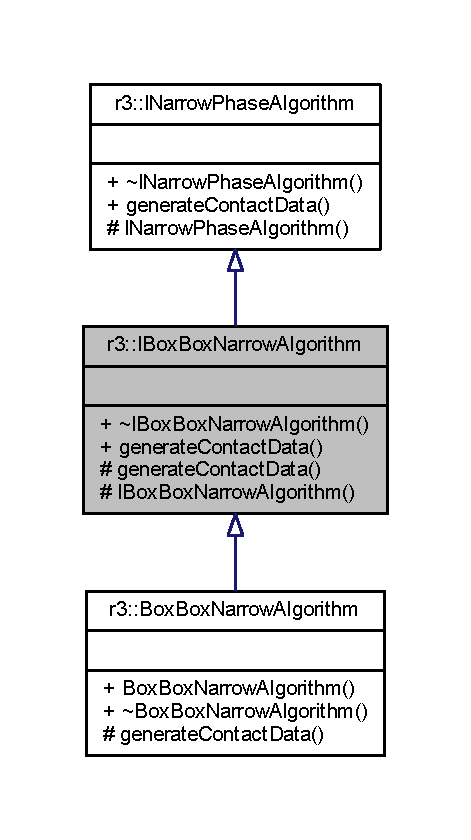
\includegraphics[width=226pt]{classr3_1_1_i_box_box_narrow_algorithm__inherit__graph}
\end{center}
\end{figure}


Collaboration diagram for r3\+:\+:I\+Box\+Box\+Narrow\+Algorithm\+:\nopagebreak
\begin{figure}[H]
\begin{center}
\leavevmode
\includegraphics[width=226pt]{classr3_1_1_i_box_box_narrow_algorithm__coll__graph}
\end{center}
\end{figure}
\subsection*{Public Member Functions}
\begin{DoxyCompactItemize}
\item 
virtual \mbox{\hyperlink{classr3_1_1_i_box_box_narrow_algorithm_a384c60f79ed845100877e62d7e2a10f4}{$\sim$\+I\+Box\+Box\+Narrow\+Algorithm}} ()
\item 
bool \mbox{\hyperlink{classr3_1_1_i_box_box_narrow_algorithm_a4b06ee2be38c248c59195082db64c3e3}{generate\+Contact\+Data}} (\mbox{\hyperlink{classr3_1_1_rigid_body}{Rigid\+Body}} $\ast$first, \mbox{\hyperlink{classr3_1_1_rigid_body}{Rigid\+Body}} $\ast$second, \mbox{\hyperlink{classr3_1_1_collision_data}{Collision\+Data}} \&collision\+Data) override final
\end{DoxyCompactItemize}
\subsection*{Protected Member Functions}
\begin{DoxyCompactItemize}
\item 
virtual bool \mbox{\hyperlink{classr3_1_1_i_box_box_narrow_algorithm_abc15898100b5ed0537e4c6ccc6610069}{generate\+Contact\+Data\+Impl}} (\mbox{\hyperlink{classr3_1_1_rigid_body}{Rigid\+Body}} $\ast$rb\+Box1, \mbox{\hyperlink{classr3_1_1_collision_box}{Collision\+Box}} $\ast$box1, \mbox{\hyperlink{classr3_1_1_rigid_body}{Rigid\+Body}} $\ast$rb\+Box2, \mbox{\hyperlink{classr3_1_1_collision_box}{Collision\+Box}} $\ast$box2, \mbox{\hyperlink{classr3_1_1_collision_data}{Collision\+Data}} \&collision\+Data)=0
\item 
\mbox{\hyperlink{classr3_1_1_i_box_box_narrow_algorithm_a9e01be1ba6e1bbd925fca03f36f06752}{I\+Box\+Box\+Narrow\+Algorithm}} ()
\end{DoxyCompactItemize}


\subsection{Constructor \& Destructor Documentation}
\mbox{\Hypertarget{classr3_1_1_i_box_box_narrow_algorithm_a384c60f79ed845100877e62d7e2a10f4}\label{classr3_1_1_i_box_box_narrow_algorithm_a384c60f79ed845100877e62d7e2a10f4}} 
\index{r3\+::\+I\+Box\+Box\+Narrow\+Algorithm@{r3\+::\+I\+Box\+Box\+Narrow\+Algorithm}!````~I\+Box\+Box\+Narrow\+Algorithm@{$\sim$\+I\+Box\+Box\+Narrow\+Algorithm}}
\index{````~I\+Box\+Box\+Narrow\+Algorithm@{$\sim$\+I\+Box\+Box\+Narrow\+Algorithm}!r3\+::\+I\+Box\+Box\+Narrow\+Algorithm@{r3\+::\+I\+Box\+Box\+Narrow\+Algorithm}}
\subsubsection{\texorpdfstring{$\sim$\+I\+Box\+Box\+Narrow\+Algorithm()}{~IBoxBoxNarrowAlgorithm()}}
{\footnotesize\ttfamily r3\+::\+I\+Box\+Box\+Narrow\+Algorithm\+::$\sim$\+I\+Box\+Box\+Narrow\+Algorithm (\begin{DoxyParamCaption}{ }\end{DoxyParamCaption})\hspace{0.3cm}{\ttfamily [virtual]}, {\ttfamily [default]}}

\mbox{\Hypertarget{classr3_1_1_i_box_box_narrow_algorithm_a9e01be1ba6e1bbd925fca03f36f06752}\label{classr3_1_1_i_box_box_narrow_algorithm_a9e01be1ba6e1bbd925fca03f36f06752}} 
\index{r3\+::\+I\+Box\+Box\+Narrow\+Algorithm@{r3\+::\+I\+Box\+Box\+Narrow\+Algorithm}!I\+Box\+Box\+Narrow\+Algorithm@{I\+Box\+Box\+Narrow\+Algorithm}}
\index{I\+Box\+Box\+Narrow\+Algorithm@{I\+Box\+Box\+Narrow\+Algorithm}!r3\+::\+I\+Box\+Box\+Narrow\+Algorithm@{r3\+::\+I\+Box\+Box\+Narrow\+Algorithm}}
\subsubsection{\texorpdfstring{I\+Box\+Box\+Narrow\+Algorithm()}{IBoxBoxNarrowAlgorithm()}}
{\footnotesize\ttfamily r3\+::\+I\+Box\+Box\+Narrow\+Algorithm\+::\+I\+Box\+Box\+Narrow\+Algorithm (\begin{DoxyParamCaption}{ }\end{DoxyParamCaption})\hspace{0.3cm}{\ttfamily [explicit]}, {\ttfamily [protected]}, {\ttfamily [default]}}



\subsection{Member Function Documentation}
\mbox{\Hypertarget{classr3_1_1_i_box_box_narrow_algorithm_a4b06ee2be38c248c59195082db64c3e3}\label{classr3_1_1_i_box_box_narrow_algorithm_a4b06ee2be38c248c59195082db64c3e3}} 
\index{r3\+::\+I\+Box\+Box\+Narrow\+Algorithm@{r3\+::\+I\+Box\+Box\+Narrow\+Algorithm}!generate\+Contact\+Data@{generate\+Contact\+Data}}
\index{generate\+Contact\+Data@{generate\+Contact\+Data}!r3\+::\+I\+Box\+Box\+Narrow\+Algorithm@{r3\+::\+I\+Box\+Box\+Narrow\+Algorithm}}
\subsubsection{\texorpdfstring{generate\+Contact\+Data()}{generateContactData()}}
{\footnotesize\ttfamily bool r3\+::\+I\+Box\+Box\+Narrow\+Algorithm\+::generate\+Contact\+Data (\begin{DoxyParamCaption}\item[{\mbox{\hyperlink{classr3_1_1_rigid_body}{Rigid\+Body}} $\ast$}]{first,  }\item[{\mbox{\hyperlink{classr3_1_1_rigid_body}{Rigid\+Body}} $\ast$}]{second,  }\item[{\mbox{\hyperlink{classr3_1_1_collision_data}{Collision\+Data}} \&}]{collision\+Data }\end{DoxyParamCaption})\hspace{0.3cm}{\ttfamily [final]}, {\ttfamily [override]}, {\ttfamily [virtual]}}



Implements \mbox{\hyperlink{classr3_1_1_i_narrow_phase_algorithm_a606fe8de5fe81ff45fedb81ca74717c3}{r3\+::\+I\+Narrow\+Phase\+Algorithm}}.

\mbox{\Hypertarget{classr3_1_1_i_box_box_narrow_algorithm_abc15898100b5ed0537e4c6ccc6610069}\label{classr3_1_1_i_box_box_narrow_algorithm_abc15898100b5ed0537e4c6ccc6610069}} 
\index{r3\+::\+I\+Box\+Box\+Narrow\+Algorithm@{r3\+::\+I\+Box\+Box\+Narrow\+Algorithm}!generate\+Contact\+Data\+Impl@{generate\+Contact\+Data\+Impl}}
\index{generate\+Contact\+Data\+Impl@{generate\+Contact\+Data\+Impl}!r3\+::\+I\+Box\+Box\+Narrow\+Algorithm@{r3\+::\+I\+Box\+Box\+Narrow\+Algorithm}}
\subsubsection{\texorpdfstring{generate\+Contact\+Data\+Impl()}{generateContactDataImpl()}}
{\footnotesize\ttfamily virtual bool r3\+::\+I\+Box\+Box\+Narrow\+Algorithm\+::generate\+Contact\+Data\+Impl (\begin{DoxyParamCaption}\item[{\mbox{\hyperlink{classr3_1_1_rigid_body}{Rigid\+Body}} $\ast$}]{rb\+Box1,  }\item[{\mbox{\hyperlink{classr3_1_1_collision_box}{Collision\+Box}} $\ast$}]{box1,  }\item[{\mbox{\hyperlink{classr3_1_1_rigid_body}{Rigid\+Body}} $\ast$}]{rb\+Box2,  }\item[{\mbox{\hyperlink{classr3_1_1_collision_box}{Collision\+Box}} $\ast$}]{box2,  }\item[{\mbox{\hyperlink{classr3_1_1_collision_data}{Collision\+Data}} \&}]{collision\+Data }\end{DoxyParamCaption})\hspace{0.3cm}{\ttfamily [protected]}, {\ttfamily [pure virtual]}}



Implemented in \mbox{\hyperlink{classr3_1_1_box_box_narrow_algorithm_a200098ad4e6e2381f58856002a2d5dec}{r3\+::\+Box\+Box\+Narrow\+Algorithm}}.



The documentation for this class was generated from the following files\+:\begin{DoxyCompactItemize}
\item 
C\+:/\+Library/\+Job/\+Projekte/\+Simulation\+Visualization/\+Rumble3\+D/\+Rumble3\+D/include/\+R3\+D/\+Rigid\+Body\+Engine/\+Collision\+Detection/\+Algorithm/\mbox{\hyperlink{_i_box_box_narrow_algorithm_8h}{I\+Box\+Box\+Narrow\+Algorithm.\+h}}\item 
C\+:/\+Library/\+Job/\+Projekte/\+Simulation\+Visualization/\+Rumble3\+D/\+Rumble3\+D/src/\+Rigid\+Body\+Engine/\+Collision\+Detection/\+Algorithm/\mbox{\hyperlink{_i_box_box_narrow_algorithm_8cpp}{I\+Box\+Box\+Narrow\+Algorithm.\+cpp}}\end{DoxyCompactItemize}

\hypertarget{classr3_1_1_i_box_sphere_narrow_algorithm}{}\section{r3\+:\+:I\+Box\+Sphere\+Narrow\+Algorithm Class Reference}
\label{classr3_1_1_i_box_sphere_narrow_algorithm}\index{r3\+::\+I\+Box\+Sphere\+Narrow\+Algorithm@{r3\+::\+I\+Box\+Sphere\+Narrow\+Algorithm}}


Interface for box-\/sphere narrow algorithms.  




{\ttfamily \#include $<$I\+Box\+Sphere\+Narrow\+Algorithm.\+h$>$}



Inheritance diagram for r3\+:\+:I\+Box\+Sphere\+Narrow\+Algorithm\+:\nopagebreak
\begin{figure}[H]
\begin{center}
\leavevmode
\includegraphics[width=239pt]{classr3_1_1_i_box_sphere_narrow_algorithm__inherit__graph}
\end{center}
\end{figure}


Collaboration diagram for r3\+:\+:I\+Box\+Sphere\+Narrow\+Algorithm\+:\nopagebreak
\begin{figure}[H]
\begin{center}
\leavevmode
\includegraphics[width=239pt]{classr3_1_1_i_box_sphere_narrow_algorithm__coll__graph}
\end{center}
\end{figure}
\subsection*{Public Member Functions}
\begin{DoxyCompactItemize}
\item 
virtual \mbox{\hyperlink{classr3_1_1_i_box_sphere_narrow_algorithm_ac70f8e99bb2deb52c1e4686ef6fafe2d}{$\sim$\+I\+Box\+Sphere\+Narrow\+Algorithm}} ()
\item 
bool \mbox{\hyperlink{classr3_1_1_i_box_sphere_narrow_algorithm_aeecdb2486c6e6cbae057466f05323bdb}{generate\+Contact\+Data}} (\mbox{\hyperlink{classr3_1_1_rigid_body}{Rigid\+Body}} $\ast$first, \mbox{\hyperlink{classr3_1_1_rigid_body}{Rigid\+Body}} $\ast$second, \mbox{\hyperlink{classr3_1_1_collision_data}{Collision\+Data}} \&collision\+Data) override final
\begin{DoxyCompactList}\small\item\em Generate contacts between two rigid bodies. \end{DoxyCompactList}\end{DoxyCompactItemize}
\subsection*{Protected Member Functions}
\begin{DoxyCompactItemize}
\item 
virtual bool \mbox{\hyperlink{classr3_1_1_i_box_sphere_narrow_algorithm_af28bcda3eb527a6ee48a3b624e5d47e0}{generate\+Contact\+Data\+Impl}} (\mbox{\hyperlink{classr3_1_1_rigid_body}{Rigid\+Body}} $\ast$rb\+Box, \mbox{\hyperlink{classr3_1_1_collision_box}{Collision\+Box}} $\ast$box, \mbox{\hyperlink{classr3_1_1_rigid_body}{Rigid\+Body}} $\ast$rb\+Sphere, \mbox{\hyperlink{classr3_1_1_collision_sphere}{Collision\+Sphere}} $\ast$sphere, \mbox{\hyperlink{classr3_1_1_collision_data}{Collision\+Data}} \&collision\+Data)=0
\item 
\mbox{\hyperlink{classr3_1_1_i_box_sphere_narrow_algorithm_ab8b57aa1583fb467fb06998487b2a5a6}{I\+Box\+Sphere\+Narrow\+Algorithm}} ()
\end{DoxyCompactItemize}


\subsection{Detailed Description}
Interface for box-\/sphere narrow algorithms. 

\subsection{Constructor \& Destructor Documentation}
\mbox{\Hypertarget{classr3_1_1_i_box_sphere_narrow_algorithm_ac70f8e99bb2deb52c1e4686ef6fafe2d}\label{classr3_1_1_i_box_sphere_narrow_algorithm_ac70f8e99bb2deb52c1e4686ef6fafe2d}} 
\index{r3\+::\+I\+Box\+Sphere\+Narrow\+Algorithm@{r3\+::\+I\+Box\+Sphere\+Narrow\+Algorithm}!````~I\+Box\+Sphere\+Narrow\+Algorithm@{$\sim$\+I\+Box\+Sphere\+Narrow\+Algorithm}}
\index{````~I\+Box\+Sphere\+Narrow\+Algorithm@{$\sim$\+I\+Box\+Sphere\+Narrow\+Algorithm}!r3\+::\+I\+Box\+Sphere\+Narrow\+Algorithm@{r3\+::\+I\+Box\+Sphere\+Narrow\+Algorithm}}
\subsubsection{\texorpdfstring{$\sim$\+I\+Box\+Sphere\+Narrow\+Algorithm()}{~IBoxSphereNarrowAlgorithm()}}
{\footnotesize\ttfamily r3\+::\+I\+Box\+Sphere\+Narrow\+Algorithm\+::$\sim$\+I\+Box\+Sphere\+Narrow\+Algorithm (\begin{DoxyParamCaption}{ }\end{DoxyParamCaption})\hspace{0.3cm}{\ttfamily [virtual]}, {\ttfamily [default]}}

\mbox{\Hypertarget{classr3_1_1_i_box_sphere_narrow_algorithm_ab8b57aa1583fb467fb06998487b2a5a6}\label{classr3_1_1_i_box_sphere_narrow_algorithm_ab8b57aa1583fb467fb06998487b2a5a6}} 
\index{r3\+::\+I\+Box\+Sphere\+Narrow\+Algorithm@{r3\+::\+I\+Box\+Sphere\+Narrow\+Algorithm}!I\+Box\+Sphere\+Narrow\+Algorithm@{I\+Box\+Sphere\+Narrow\+Algorithm}}
\index{I\+Box\+Sphere\+Narrow\+Algorithm@{I\+Box\+Sphere\+Narrow\+Algorithm}!r3\+::\+I\+Box\+Sphere\+Narrow\+Algorithm@{r3\+::\+I\+Box\+Sphere\+Narrow\+Algorithm}}
\subsubsection{\texorpdfstring{I\+Box\+Sphere\+Narrow\+Algorithm()}{IBoxSphereNarrowAlgorithm()}}
{\footnotesize\ttfamily r3\+::\+I\+Box\+Sphere\+Narrow\+Algorithm\+::\+I\+Box\+Sphere\+Narrow\+Algorithm (\begin{DoxyParamCaption}{ }\end{DoxyParamCaption})\hspace{0.3cm}{\ttfamily [explicit]}, {\ttfamily [protected]}, {\ttfamily [default]}}



\subsection{Member Function Documentation}
\mbox{\Hypertarget{classr3_1_1_i_box_sphere_narrow_algorithm_aeecdb2486c6e6cbae057466f05323bdb}\label{classr3_1_1_i_box_sphere_narrow_algorithm_aeecdb2486c6e6cbae057466f05323bdb}} 
\index{r3\+::\+I\+Box\+Sphere\+Narrow\+Algorithm@{r3\+::\+I\+Box\+Sphere\+Narrow\+Algorithm}!generate\+Contact\+Data@{generate\+Contact\+Data}}
\index{generate\+Contact\+Data@{generate\+Contact\+Data}!r3\+::\+I\+Box\+Sphere\+Narrow\+Algorithm@{r3\+::\+I\+Box\+Sphere\+Narrow\+Algorithm}}
\subsubsection{\texorpdfstring{generate\+Contact\+Data()}{generateContactData()}}
{\footnotesize\ttfamily bool r3\+::\+I\+Box\+Sphere\+Narrow\+Algorithm\+::generate\+Contact\+Data (\begin{DoxyParamCaption}\item[{\mbox{\hyperlink{classr3_1_1_rigid_body}{Rigid\+Body}} $\ast$}]{first,  }\item[{\mbox{\hyperlink{classr3_1_1_rigid_body}{Rigid\+Body}} $\ast$}]{second,  }\item[{\mbox{\hyperlink{classr3_1_1_collision_data}{Collision\+Data}} \&}]{collision\+Data }\end{DoxyParamCaption})\hspace{0.3cm}{\ttfamily [final]}, {\ttfamily [override]}, {\ttfamily [virtual]}}



Generate contacts between two rigid bodies. 


\begin{DoxyParams}{Parameters}
{\em first} & The first participating rigid body. \\
\hline
{\em second} & The second participating rigid body. \\
\hline
{\em collision\+Data} & All newly generated contacts will be put in here. \\
\hline
\end{DoxyParams}
\begin{DoxyReturn}{Returns}
True if new contacts have been generated, false otherwise. 
\end{DoxyReturn}


Implements \mbox{\hyperlink{classr3_1_1_i_narrow_phase_algorithm_a606fe8de5fe81ff45fedb81ca74717c3}{r3\+::\+I\+Narrow\+Phase\+Algorithm}}.

\mbox{\Hypertarget{classr3_1_1_i_box_sphere_narrow_algorithm_af28bcda3eb527a6ee48a3b624e5d47e0}\label{classr3_1_1_i_box_sphere_narrow_algorithm_af28bcda3eb527a6ee48a3b624e5d47e0}} 
\index{r3\+::\+I\+Box\+Sphere\+Narrow\+Algorithm@{r3\+::\+I\+Box\+Sphere\+Narrow\+Algorithm}!generate\+Contact\+Data\+Impl@{generate\+Contact\+Data\+Impl}}
\index{generate\+Contact\+Data\+Impl@{generate\+Contact\+Data\+Impl}!r3\+::\+I\+Box\+Sphere\+Narrow\+Algorithm@{r3\+::\+I\+Box\+Sphere\+Narrow\+Algorithm}}
\subsubsection{\texorpdfstring{generate\+Contact\+Data\+Impl()}{generateContactDataImpl()}}
{\footnotesize\ttfamily virtual bool r3\+::\+I\+Box\+Sphere\+Narrow\+Algorithm\+::generate\+Contact\+Data\+Impl (\begin{DoxyParamCaption}\item[{\mbox{\hyperlink{classr3_1_1_rigid_body}{Rigid\+Body}} $\ast$}]{rb\+Box,  }\item[{\mbox{\hyperlink{classr3_1_1_collision_box}{Collision\+Box}} $\ast$}]{box,  }\item[{\mbox{\hyperlink{classr3_1_1_rigid_body}{Rigid\+Body}} $\ast$}]{rb\+Sphere,  }\item[{\mbox{\hyperlink{classr3_1_1_collision_sphere}{Collision\+Sphere}} $\ast$}]{sphere,  }\item[{\mbox{\hyperlink{classr3_1_1_collision_data}{Collision\+Data}} \&}]{collision\+Data }\end{DoxyParamCaption})\hspace{0.3cm}{\ttfamily [protected]}, {\ttfamily [pure virtual]}}



Implemented in \mbox{\hyperlink{classr3_1_1_box_sphere_narrow_algorithm_a2fc345fdec27e85f0e569afa0d500865}{r3\+::\+Box\+Sphere\+Narrow\+Algorithm}}.



The documentation for this class was generated from the following files\+:\begin{DoxyCompactItemize}
\item 
D\+:/\+Library/\+Documents/\+Job/\+Forschungsmaster/\+Projekte/\+Simulation\+Visualization/\+Rumble3\+D/\+Rumble3\+D/include/\+R3\+D/\+Rigid\+Body\+Engine/\+Collision\+Detection/\+Algorithm/\mbox{\hyperlink{_i_box_sphere_narrow_algorithm_8h}{I\+Box\+Sphere\+Narrow\+Algorithm.\+h}}\item 
D\+:/\+Library/\+Documents/\+Job/\+Forschungsmaster/\+Projekte/\+Simulation\+Visualization/\+Rumble3\+D/\+Rumble3\+D/src/\+Rigid\+Body\+Engine/\+Collision\+Detection/\+Algorithm/\mbox{\hyperlink{_i_box_sphere_narrow_algorithm_8cpp}{I\+Box\+Sphere\+Narrow\+Algorithm.\+cpp}}\end{DoxyCompactItemize}

\hypertarget{classr3_1_1_i_broad_phase_filter}{}\section{r3\+:\+:I\+Broad\+Phase\+Filter Class Reference}
\label{classr3_1_1_i_broad_phase_filter}\index{r3\+::\+I\+Broad\+Phase\+Filter@{r3\+::\+I\+Broad\+Phase\+Filter}}


{\ttfamily \#include $<$I\+Broad\+Phase\+Filter.\+h$>$}



Inheritance diagram for r3\+:\+:I\+Broad\+Phase\+Filter\+:\nopagebreak
\begin{figure}[H]
\begin{center}
\leavevmode
\includegraphics[width=195pt]{classr3_1_1_i_broad_phase_filter__inherit__graph}
\end{center}
\end{figure}


Collaboration diagram for r3\+:\+:I\+Broad\+Phase\+Filter\+:\nopagebreak
\begin{figure}[H]
\begin{center}
\leavevmode
\includegraphics[width=195pt]{classr3_1_1_i_broad_phase_filter__coll__graph}
\end{center}
\end{figure}
\subsection*{Public Member Functions}
\begin{DoxyCompactItemize}
\item 
virtual \mbox{\hyperlink{classr3_1_1_i_broad_phase_filter_af6cd5cfcf4487d97916debae0011244f}{$\sim$\+I\+Broad\+Phase\+Filter}} ()
\item 
virtual void \mbox{\hyperlink{classr3_1_1_i_broad_phase_filter_a5f437f6390a8f10bf96d72e35e3b4432}{generate\+Collisions}} (const std\+::vector$<$ \mbox{\hyperlink{classr3_1_1_rigid_body}{Rigid\+Body}} $\ast$$>$ \&rigid\+Bodies, \mbox{\hyperlink{classr3_1_1_fixed_size_container}{Fixed\+Size\+Container}}$<$ \mbox{\hyperlink{classr3_1_1_collision_pair}{Collision\+Pair}} $>$ \&data)=0
\end{DoxyCompactItemize}
\subsection*{Protected Member Functions}
\begin{DoxyCompactItemize}
\item 
\mbox{\hyperlink{classr3_1_1_i_broad_phase_filter_ab1eb5dc44548078aa0716eedbab8ac11}{I\+Broad\+Phase\+Filter}} ()
\end{DoxyCompactItemize}


\subsection{Constructor \& Destructor Documentation}
\mbox{\Hypertarget{classr3_1_1_i_broad_phase_filter_af6cd5cfcf4487d97916debae0011244f}\label{classr3_1_1_i_broad_phase_filter_af6cd5cfcf4487d97916debae0011244f}} 
\index{r3\+::\+I\+Broad\+Phase\+Filter@{r3\+::\+I\+Broad\+Phase\+Filter}!````~I\+Broad\+Phase\+Filter@{$\sim$\+I\+Broad\+Phase\+Filter}}
\index{````~I\+Broad\+Phase\+Filter@{$\sim$\+I\+Broad\+Phase\+Filter}!r3\+::\+I\+Broad\+Phase\+Filter@{r3\+::\+I\+Broad\+Phase\+Filter}}
\subsubsection{\texorpdfstring{$\sim$\+I\+Broad\+Phase\+Filter()}{~IBroadPhaseFilter()}}
{\footnotesize\ttfamily r3\+::\+I\+Broad\+Phase\+Filter\+::$\sim$\+I\+Broad\+Phase\+Filter (\begin{DoxyParamCaption}{ }\end{DoxyParamCaption})\hspace{0.3cm}{\ttfamily [virtual]}, {\ttfamily [default]}}

\mbox{\Hypertarget{classr3_1_1_i_broad_phase_filter_ab1eb5dc44548078aa0716eedbab8ac11}\label{classr3_1_1_i_broad_phase_filter_ab1eb5dc44548078aa0716eedbab8ac11}} 
\index{r3\+::\+I\+Broad\+Phase\+Filter@{r3\+::\+I\+Broad\+Phase\+Filter}!I\+Broad\+Phase\+Filter@{I\+Broad\+Phase\+Filter}}
\index{I\+Broad\+Phase\+Filter@{I\+Broad\+Phase\+Filter}!r3\+::\+I\+Broad\+Phase\+Filter@{r3\+::\+I\+Broad\+Phase\+Filter}}
\subsubsection{\texorpdfstring{I\+Broad\+Phase\+Filter()}{IBroadPhaseFilter()}}
{\footnotesize\ttfamily r3\+::\+I\+Broad\+Phase\+Filter\+::\+I\+Broad\+Phase\+Filter (\begin{DoxyParamCaption}{ }\end{DoxyParamCaption})\hspace{0.3cm}{\ttfamily [explicit]}, {\ttfamily [protected]}, {\ttfamily [default]}}



\subsection{Member Function Documentation}
\mbox{\Hypertarget{classr3_1_1_i_broad_phase_filter_a5f437f6390a8f10bf96d72e35e3b4432}\label{classr3_1_1_i_broad_phase_filter_a5f437f6390a8f10bf96d72e35e3b4432}} 
\index{r3\+::\+I\+Broad\+Phase\+Filter@{r3\+::\+I\+Broad\+Phase\+Filter}!generate\+Collisions@{generate\+Collisions}}
\index{generate\+Collisions@{generate\+Collisions}!r3\+::\+I\+Broad\+Phase\+Filter@{r3\+::\+I\+Broad\+Phase\+Filter}}
\subsubsection{\texorpdfstring{generate\+Collisions()}{generateCollisions()}}
{\footnotesize\ttfamily virtual void r3\+::\+I\+Broad\+Phase\+Filter\+::generate\+Collisions (\begin{DoxyParamCaption}\item[{const std\+::vector$<$ \mbox{\hyperlink{classr3_1_1_rigid_body}{Rigid\+Body}} $\ast$$>$ \&}]{rigid\+Bodies,  }\item[{\mbox{\hyperlink{classr3_1_1_fixed_size_container}{Fixed\+Size\+Container}}$<$ \mbox{\hyperlink{classr3_1_1_collision_pair}{Collision\+Pair}} $>$ \&}]{data }\end{DoxyParamCaption})\hspace{0.3cm}{\ttfamily [pure virtual]}}

Conservatively check, which rigid body pairs might collide. These collisions can be false positives, but there should never be false negatives. \begin{DoxyReturn}{Returns}
A number of possible collisions. 
\end{DoxyReturn}


Implemented in \mbox{\hyperlink{classr3_1_1_broad_phase_filter_a0435dc6468401e32bf151f84f52e80f8}{r3\+::\+Broad\+Phase\+Filter}}.



The documentation for this class was generated from the following files\+:\begin{DoxyCompactItemize}
\item 
C\+:/\+Library/\+Job/\+Projekte/\+Simulation\+Visualization/\+Rumble3\+D/\+Rumble3\+D/include/\+R3\+D/\+Rigid\+Body\+Engine/\+Collision\+Detection/\mbox{\hyperlink{_i_broad_phase_filter_8h}{I\+Broad\+Phase\+Filter.\+h}}\item 
C\+:/\+Library/\+Job/\+Projekte/\+Simulation\+Visualization/\+Rumble3\+D/\+Rumble3\+D/src/\+Rigid\+Body\+Engine/\+Collision\+Detection/\mbox{\hyperlink{_i_broad_phase_filter_8cpp}{I\+Broad\+Phase\+Filter.\+cpp}}\end{DoxyCompactItemize}

\hypertarget{classr3_1_1_i_collision_resolution_filter}{}\section{r3\+:\+:I\+Collision\+Resolution\+Filter Class Reference}
\label{classr3_1_1_i_collision_resolution_filter}\index{r3\+::\+I\+Collision\+Resolution\+Filter@{r3\+::\+I\+Collision\+Resolution\+Filter}}


{\ttfamily \#include $<$I\+Collision\+Resolution\+Filter.\+h$>$}



Inheritance diagram for r3\+:\+:I\+Collision\+Resolution\+Filter\+:\nopagebreak
\begin{figure}[H]
\begin{center}
\leavevmode
\includegraphics[width=350pt]{classr3_1_1_i_collision_resolution_filter__inherit__graph}
\end{center}
\end{figure}


Collaboration diagram for r3\+:\+:I\+Collision\+Resolution\+Filter\+:\nopagebreak
\begin{figure}[H]
\begin{center}
\leavevmode
\includegraphics[width=224pt]{classr3_1_1_i_collision_resolution_filter__coll__graph}
\end{center}
\end{figure}
\subsection*{Public Member Functions}
\begin{DoxyCompactItemize}
\item 
virtual \mbox{\hyperlink{classr3_1_1_i_collision_resolution_filter_a89b3382d573308a790d436b9713b02ed}{$\sim$\+I\+Collision\+Resolution\+Filter}} ()
\item 
virtual void \mbox{\hyperlink{classr3_1_1_i_collision_resolution_filter_a87ef2579e2acaaadef4cd8f9a20005ce}{resolve}} (\mbox{\hyperlink{classr3_1_1_collision_data}{Collision\+Data}} \&collision\+Data, \mbox{\hyperlink{namespacer3_ab2016b3e3f743fb735afce242f0dc1eb}{real}} time\+Delta)=0
\end{DoxyCompactItemize}
\subsection*{Protected Member Functions}
\begin{DoxyCompactItemize}
\item 
\mbox{\hyperlink{classr3_1_1_i_collision_resolution_filter_ab2dcf60620e28db288abf19bdeeb11ad}{I\+Collision\+Resolution\+Filter}} ()
\end{DoxyCompactItemize}


\subsection{Constructor \& Destructor Documentation}
\mbox{\Hypertarget{classr3_1_1_i_collision_resolution_filter_a89b3382d573308a790d436b9713b02ed}\label{classr3_1_1_i_collision_resolution_filter_a89b3382d573308a790d436b9713b02ed}} 
\index{r3\+::\+I\+Collision\+Resolution\+Filter@{r3\+::\+I\+Collision\+Resolution\+Filter}!````~I\+Collision\+Resolution\+Filter@{$\sim$\+I\+Collision\+Resolution\+Filter}}
\index{````~I\+Collision\+Resolution\+Filter@{$\sim$\+I\+Collision\+Resolution\+Filter}!r3\+::\+I\+Collision\+Resolution\+Filter@{r3\+::\+I\+Collision\+Resolution\+Filter}}
\subsubsection{\texorpdfstring{$\sim$\+I\+Collision\+Resolution\+Filter()}{~ICollisionResolutionFilter()}}
{\footnotesize\ttfamily r3\+::\+I\+Collision\+Resolution\+Filter\+::$\sim$\+I\+Collision\+Resolution\+Filter (\begin{DoxyParamCaption}{ }\end{DoxyParamCaption})\hspace{0.3cm}{\ttfamily [virtual]}, {\ttfamily [default]}}

\mbox{\Hypertarget{classr3_1_1_i_collision_resolution_filter_ab2dcf60620e28db288abf19bdeeb11ad}\label{classr3_1_1_i_collision_resolution_filter_ab2dcf60620e28db288abf19bdeeb11ad}} 
\index{r3\+::\+I\+Collision\+Resolution\+Filter@{r3\+::\+I\+Collision\+Resolution\+Filter}!I\+Collision\+Resolution\+Filter@{I\+Collision\+Resolution\+Filter}}
\index{I\+Collision\+Resolution\+Filter@{I\+Collision\+Resolution\+Filter}!r3\+::\+I\+Collision\+Resolution\+Filter@{r3\+::\+I\+Collision\+Resolution\+Filter}}
\subsubsection{\texorpdfstring{I\+Collision\+Resolution\+Filter()}{ICollisionResolutionFilter()}}
{\footnotesize\ttfamily r3\+::\+I\+Collision\+Resolution\+Filter\+::\+I\+Collision\+Resolution\+Filter (\begin{DoxyParamCaption}{ }\end{DoxyParamCaption})\hspace{0.3cm}{\ttfamily [explicit]}, {\ttfamily [protected]}, {\ttfamily [default]}}



\subsection{Member Function Documentation}
\mbox{\Hypertarget{classr3_1_1_i_collision_resolution_filter_a87ef2579e2acaaadef4cd8f9a20005ce}\label{classr3_1_1_i_collision_resolution_filter_a87ef2579e2acaaadef4cd8f9a20005ce}} 
\index{r3\+::\+I\+Collision\+Resolution\+Filter@{r3\+::\+I\+Collision\+Resolution\+Filter}!resolve@{resolve}}
\index{resolve@{resolve}!r3\+::\+I\+Collision\+Resolution\+Filter@{r3\+::\+I\+Collision\+Resolution\+Filter}}
\subsubsection{\texorpdfstring{resolve()}{resolve()}}
{\footnotesize\ttfamily virtual void r3\+::\+I\+Collision\+Resolution\+Filter\+::resolve (\begin{DoxyParamCaption}\item[{\mbox{\hyperlink{classr3_1_1_collision_data}{Collision\+Data}} \&}]{collision\+Data,  }\item[{\mbox{\hyperlink{namespacer3_ab2016b3e3f743fb735afce242f0dc1eb}{real}}}]{time\+Delta }\end{DoxyParamCaption})\hspace{0.3cm}{\ttfamily [pure virtual]}}



Implemented in \mbox{\hyperlink{classr3_1_1_friction_resolver_af26a84959e95749088f713176ec3c096}{r3\+::\+Friction\+Resolver}}, \mbox{\hyperlink{classr3_1_1_interpenetration_resolver_a7c896a7e8e0321c9f26b3d9c616d16ee}{r3\+::\+Interpenetration\+Resolver}}, and \mbox{\hyperlink{classr3_1_1_velocity_resolver_a93e8859d1ab3407b073328a58b7caeef}{r3\+::\+Velocity\+Resolver}}.



The documentation for this class was generated from the following files\+:\begin{DoxyCompactItemize}
\item 
D\+:/\+Library/\+Documents/\+Job/\+Forschungsmaster/\+Projekte/\+Simulation\+Visualization/\+Rumble3\+D/\+Rumble3\+D/include/\+R3\+D/\+Rigid\+Body\+Engine/\+Collision\+Resolution/\mbox{\hyperlink{_i_collision_resolution_filter_8h}{I\+Collision\+Resolution\+Filter.\+h}}\item 
D\+:/\+Library/\+Documents/\+Job/\+Forschungsmaster/\+Projekte/\+Simulation\+Visualization/\+Rumble3\+D/\+Rumble3\+D/src/\+Rigid\+Body\+Engine/\+Collision\+Resolution/\mbox{\hyperlink{_i_collision_resolution_filter_8cpp}{I\+Collision\+Resolution\+Filter.\+cpp}}\end{DoxyCompactItemize}

\hypertarget{classr3_1_1_i_collision_resolver_access}{}\section{r3\+:\+:I\+Collision\+Resolver\+Access Class Reference}
\label{classr3_1_1_i_collision_resolver_access}\index{r3\+::\+I\+Collision\+Resolver\+Access@{r3\+::\+I\+Collision\+Resolver\+Access}}


{\ttfamily \#include $<$I\+Collision\+Resolver\+Access.\+h$>$}



Inheritance diagram for r3\+:\+:I\+Collision\+Resolver\+Access\+:\nopagebreak
\begin{figure}[H]
\begin{center}
\leavevmode
\includegraphics[width=226pt]{classr3_1_1_i_collision_resolver_access__inherit__graph}
\end{center}
\end{figure}


Collaboration diagram for r3\+:\+:I\+Collision\+Resolver\+Access\+:\nopagebreak
\begin{figure}[H]
\begin{center}
\leavevmode
\includegraphics[width=226pt]{classr3_1_1_i_collision_resolver_access__coll__graph}
\end{center}
\end{figure}
\subsection*{Public Member Functions}
\begin{DoxyCompactItemize}
\item 
virtual \mbox{\hyperlink{classr3_1_1_i_collision_resolver_access_a56e8e69db0a57cb22e3c8defa8502b30}{$\sim$\+I\+Collision\+Resolver\+Access}} ()
\item 
virtual void \mbox{\hyperlink{classr3_1_1_i_collision_resolver_access_a266dfbc4c421a7c3429ef474d63fd941}{resolve\+Collisions}} (\mbox{\hyperlink{classr3_1_1_collision_data}{Collision\+Data}} \&collision\+Data, \mbox{\hyperlink{namespacer3_ab2016b3e3f743fb735afce242f0dc1eb}{real}} time\+Delta)=0
\end{DoxyCompactItemize}
\subsection*{Protected Member Functions}
\begin{DoxyCompactItemize}
\item 
\mbox{\hyperlink{classr3_1_1_i_collision_resolver_access_ade62636ccefb20b027eef0ff272d6d48}{I\+Collision\+Resolver\+Access}} ()
\end{DoxyCompactItemize}


\subsection{Constructor \& Destructor Documentation}
\mbox{\Hypertarget{classr3_1_1_i_collision_resolver_access_a56e8e69db0a57cb22e3c8defa8502b30}\label{classr3_1_1_i_collision_resolver_access_a56e8e69db0a57cb22e3c8defa8502b30}} 
\index{r3\+::\+I\+Collision\+Resolver\+Access@{r3\+::\+I\+Collision\+Resolver\+Access}!````~I\+Collision\+Resolver\+Access@{$\sim$\+I\+Collision\+Resolver\+Access}}
\index{````~I\+Collision\+Resolver\+Access@{$\sim$\+I\+Collision\+Resolver\+Access}!r3\+::\+I\+Collision\+Resolver\+Access@{r3\+::\+I\+Collision\+Resolver\+Access}}
\subsubsection{\texorpdfstring{$\sim$\+I\+Collision\+Resolver\+Access()}{~ICollisionResolverAccess()}}
{\footnotesize\ttfamily r3\+::\+I\+Collision\+Resolver\+Access\+::$\sim$\+I\+Collision\+Resolver\+Access (\begin{DoxyParamCaption}{ }\end{DoxyParamCaption})\hspace{0.3cm}{\ttfamily [virtual]}, {\ttfamily [default]}}

\mbox{\Hypertarget{classr3_1_1_i_collision_resolver_access_ade62636ccefb20b027eef0ff272d6d48}\label{classr3_1_1_i_collision_resolver_access_ade62636ccefb20b027eef0ff272d6d48}} 
\index{r3\+::\+I\+Collision\+Resolver\+Access@{r3\+::\+I\+Collision\+Resolver\+Access}!I\+Collision\+Resolver\+Access@{I\+Collision\+Resolver\+Access}}
\index{I\+Collision\+Resolver\+Access@{I\+Collision\+Resolver\+Access}!r3\+::\+I\+Collision\+Resolver\+Access@{r3\+::\+I\+Collision\+Resolver\+Access}}
\subsubsection{\texorpdfstring{I\+Collision\+Resolver\+Access()}{ICollisionResolverAccess()}}
{\footnotesize\ttfamily r3\+::\+I\+Collision\+Resolver\+Access\+::\+I\+Collision\+Resolver\+Access (\begin{DoxyParamCaption}{ }\end{DoxyParamCaption})\hspace{0.3cm}{\ttfamily [explicit]}, {\ttfamily [protected]}, {\ttfamily [default]}}



\subsection{Member Function Documentation}
\mbox{\Hypertarget{classr3_1_1_i_collision_resolver_access_a266dfbc4c421a7c3429ef474d63fd941}\label{classr3_1_1_i_collision_resolver_access_a266dfbc4c421a7c3429ef474d63fd941}} 
\index{r3\+::\+I\+Collision\+Resolver\+Access@{r3\+::\+I\+Collision\+Resolver\+Access}!resolve\+Collisions@{resolve\+Collisions}}
\index{resolve\+Collisions@{resolve\+Collisions}!r3\+::\+I\+Collision\+Resolver\+Access@{r3\+::\+I\+Collision\+Resolver\+Access}}
\subsubsection{\texorpdfstring{resolve\+Collisions()}{resolveCollisions()}}
{\footnotesize\ttfamily virtual void r3\+::\+I\+Collision\+Resolver\+Access\+::resolve\+Collisions (\begin{DoxyParamCaption}\item[{\mbox{\hyperlink{classr3_1_1_collision_data}{Collision\+Data}} \&}]{collision\+Data,  }\item[{\mbox{\hyperlink{namespacer3_ab2016b3e3f743fb735afce242f0dc1eb}{real}}}]{time\+Delta }\end{DoxyParamCaption})\hspace{0.3cm}{\ttfamily [pure virtual]}}



Implemented in \mbox{\hyperlink{classr3_1_1_collision_resolver_a134da5221d60b34c568f7de29c9d0a58}{r3\+::\+Collision\+Resolver}}.



The documentation for this class was generated from the following files\+:\begin{DoxyCompactItemize}
\item 
C\+:/\+Library/\+Job/\+Projekte/\+Simulation\+Visualization/\+Rumble3\+D/\+Rumble3\+D/include/\+R3\+D/\+Rigid\+Body\+Engine/\+Collision\+Resolution/\mbox{\hyperlink{_i_collision_resolver_access_8h}{I\+Collision\+Resolver\+Access.\+h}}\item 
C\+:/\+Library/\+Job/\+Projekte/\+Simulation\+Visualization/\+Rumble3\+D/\+Rumble3\+D/src/\+Rigid\+Body\+Engine/\+Collision\+Resolution/\mbox{\hyperlink{_i_collision_resolver_access_8cpp}{I\+Collision\+Resolver\+Access.\+cpp}}\end{DoxyCompactItemize}

\hypertarget{classr3_1_1_i_computation_interface}{}\section{r3\+:\+:I\+Computation\+Interface Class Reference}
\label{classr3_1_1_i_computation_interface}\index{r3\+::\+I\+Computation\+Interface@{r3\+::\+I\+Computation\+Interface}}


Interface used by physics modules to accomplish their tasks.  




{\ttfamily \#include $<$I\+Computation\+Interface.\+h$>$}



Inheritance diagram for r3\+:\+:I\+Computation\+Interface\+:\nopagebreak
\begin{figure}[H]
\begin{center}
\leavevmode
\includegraphics[width=350pt]{classr3_1_1_i_computation_interface__inherit__graph}
\end{center}
\end{figure}


Collaboration diagram for r3\+:\+:I\+Computation\+Interface\+:\nopagebreak
\begin{figure}[H]
\begin{center}
\leavevmode
\includegraphics[width=211pt]{classr3_1_1_i_computation_interface__coll__graph}
\end{center}
\end{figure}
\subsection*{Public Member Functions}
\begin{DoxyCompactItemize}
\item 
virtual \mbox{\hyperlink{classr3_1_1_i_computation_interface_a88c5734b5636745f0200c03adac30994}{$\sim$\+I\+Computation\+Interface}} ()
\item 
virtual void \mbox{\hyperlink{classr3_1_1_i_computation_interface_a430ebc9cb8d4ba064ac6a032ef07edd7}{on\+Begin}} ()=0
\begin{DoxyCompactList}\small\item\em Called at the start of a physics step. \end{DoxyCompactList}\item 
virtual void \mbox{\hyperlink{classr3_1_1_i_computation_interface_aaa12bcc35005f32a1984b38de97696cb}{step}} (\mbox{\hyperlink{namespacer3_ab2016b3e3f743fb735afce242f0dc1eb}{real}} time\+Delta)=0
\begin{DoxyCompactList}\small\item\em Used to calculate changes. \end{DoxyCompactList}\item 
virtual void \mbox{\hyperlink{classr3_1_1_i_computation_interface_a162250f2b6efbd85460bd0f780d42cff}{integrate}} (\mbox{\hyperlink{namespacer3_ab2016b3e3f743fb735afce242f0dc1eb}{real}} time\+Delta)=0
\begin{DoxyCompactList}\small\item\em Used to apply changes. \end{DoxyCompactList}\item 
virtual void \mbox{\hyperlink{classr3_1_1_i_computation_interface_acae0c5fada7e414c74fe6f5a8f4a6c7d}{on\+End}} ()=0
\begin{DoxyCompactList}\small\item\em Called at the end of a physics step. \end{DoxyCompactList}\item 
virtual void \mbox{\hyperlink{classr3_1_1_i_computation_interface_a6069989c54ffd4e714788d0968851007}{reset}} ()=0
\begin{DoxyCompactList}\small\item\em Resets a computation interface to its start state. \end{DoxyCompactList}\end{DoxyCompactItemize}
\subsection*{Protected Member Functions}
\begin{DoxyCompactItemize}
\item 
\mbox{\hyperlink{classr3_1_1_i_computation_interface_aa7ec35b2ab0cccd1a94ebdfeccc7bb43}{I\+Computation\+Interface}} ()
\end{DoxyCompactItemize}


\subsection{Detailed Description}
Interface used by physics modules to accomplish their tasks. 

\subsection{Constructor \& Destructor Documentation}
\mbox{\Hypertarget{classr3_1_1_i_computation_interface_a88c5734b5636745f0200c03adac30994}\label{classr3_1_1_i_computation_interface_a88c5734b5636745f0200c03adac30994}} 
\index{r3\+::\+I\+Computation\+Interface@{r3\+::\+I\+Computation\+Interface}!````~I\+Computation\+Interface@{$\sim$\+I\+Computation\+Interface}}
\index{````~I\+Computation\+Interface@{$\sim$\+I\+Computation\+Interface}!r3\+::\+I\+Computation\+Interface@{r3\+::\+I\+Computation\+Interface}}
\subsubsection{\texorpdfstring{$\sim$\+I\+Computation\+Interface()}{~IComputationInterface()}}
{\footnotesize\ttfamily r3\+::\+I\+Computation\+Interface\+::$\sim$\+I\+Computation\+Interface (\begin{DoxyParamCaption}{ }\end{DoxyParamCaption})\hspace{0.3cm}{\ttfamily [virtual]}, {\ttfamily [default]}}

\mbox{\Hypertarget{classr3_1_1_i_computation_interface_aa7ec35b2ab0cccd1a94ebdfeccc7bb43}\label{classr3_1_1_i_computation_interface_aa7ec35b2ab0cccd1a94ebdfeccc7bb43}} 
\index{r3\+::\+I\+Computation\+Interface@{r3\+::\+I\+Computation\+Interface}!I\+Computation\+Interface@{I\+Computation\+Interface}}
\index{I\+Computation\+Interface@{I\+Computation\+Interface}!r3\+::\+I\+Computation\+Interface@{r3\+::\+I\+Computation\+Interface}}
\subsubsection{\texorpdfstring{I\+Computation\+Interface()}{IComputationInterface()}}
{\footnotesize\ttfamily r3\+::\+I\+Computation\+Interface\+::\+I\+Computation\+Interface (\begin{DoxyParamCaption}{ }\end{DoxyParamCaption})\hspace{0.3cm}{\ttfamily [explicit]}, {\ttfamily [protected]}, {\ttfamily [default]}}



\subsection{Member Function Documentation}
\mbox{\Hypertarget{classr3_1_1_i_computation_interface_a162250f2b6efbd85460bd0f780d42cff}\label{classr3_1_1_i_computation_interface_a162250f2b6efbd85460bd0f780d42cff}} 
\index{r3\+::\+I\+Computation\+Interface@{r3\+::\+I\+Computation\+Interface}!integrate@{integrate}}
\index{integrate@{integrate}!r3\+::\+I\+Computation\+Interface@{r3\+::\+I\+Computation\+Interface}}
\subsubsection{\texorpdfstring{integrate()}{integrate()}}
{\footnotesize\ttfamily void r3\+::\+I\+Computation\+Interface\+::integrate (\begin{DoxyParamCaption}\item[{\mbox{\hyperlink{namespacer3_ab2016b3e3f743fb735afce242f0dc1eb}{real}}}]{time\+Delta }\end{DoxyParamCaption})\hspace{0.3cm}{\ttfamily [pure virtual]}}



Used to apply changes. 


\begin{DoxyParams}{Parameters}
{\em time\+Delta} & The time step of the physics step. \\
\hline
\end{DoxyParams}


Implemented in \mbox{\hyperlink{classr3_1_1_default_particle_engine_c_i_a4603707afe6c841a83294a46ea4a1c62}{r3\+::\+Default\+Particle\+Engine\+CI}}, and \mbox{\hyperlink{classr3_1_1_default_rigid_body_engine_c_i_a4b79e7e4bc76eedcad7ef5c4777b9d33}{r3\+::\+Default\+Rigid\+Body\+Engine\+CI}}.

\mbox{\Hypertarget{classr3_1_1_i_computation_interface_a430ebc9cb8d4ba064ac6a032ef07edd7}\label{classr3_1_1_i_computation_interface_a430ebc9cb8d4ba064ac6a032ef07edd7}} 
\index{r3\+::\+I\+Computation\+Interface@{r3\+::\+I\+Computation\+Interface}!on\+Begin@{on\+Begin}}
\index{on\+Begin@{on\+Begin}!r3\+::\+I\+Computation\+Interface@{r3\+::\+I\+Computation\+Interface}}
\subsubsection{\texorpdfstring{on\+Begin()}{onBegin()}}
{\footnotesize\ttfamily void r3\+::\+I\+Computation\+Interface\+::on\+Begin (\begin{DoxyParamCaption}{ }\end{DoxyParamCaption})\hspace{0.3cm}{\ttfamily [pure virtual]}}



Called at the start of a physics step. 



Implemented in \mbox{\hyperlink{classr3_1_1_default_particle_engine_c_i_aaf2e9ca87bff5e48c8eb59384e9cf180}{r3\+::\+Default\+Particle\+Engine\+CI}}, and \mbox{\hyperlink{classr3_1_1_default_rigid_body_engine_c_i_a5d9e40ea40845499f01081d21cd9ff64}{r3\+::\+Default\+Rigid\+Body\+Engine\+CI}}.

\mbox{\Hypertarget{classr3_1_1_i_computation_interface_acae0c5fada7e414c74fe6f5a8f4a6c7d}\label{classr3_1_1_i_computation_interface_acae0c5fada7e414c74fe6f5a8f4a6c7d}} 
\index{r3\+::\+I\+Computation\+Interface@{r3\+::\+I\+Computation\+Interface}!on\+End@{on\+End}}
\index{on\+End@{on\+End}!r3\+::\+I\+Computation\+Interface@{r3\+::\+I\+Computation\+Interface}}
\subsubsection{\texorpdfstring{on\+End()}{onEnd()}}
{\footnotesize\ttfamily void r3\+::\+I\+Computation\+Interface\+::on\+End (\begin{DoxyParamCaption}{ }\end{DoxyParamCaption})\hspace{0.3cm}{\ttfamily [pure virtual]}}



Called at the end of a physics step. 



Implemented in \mbox{\hyperlink{classr3_1_1_default_particle_engine_c_i_a6a34c77436d8133560eaa7366c740119}{r3\+::\+Default\+Particle\+Engine\+CI}}, and \mbox{\hyperlink{classr3_1_1_default_rigid_body_engine_c_i_ad7746126ebd5aab4cfc352dd9facabb2}{r3\+::\+Default\+Rigid\+Body\+Engine\+CI}}.

\mbox{\Hypertarget{classr3_1_1_i_computation_interface_a6069989c54ffd4e714788d0968851007}\label{classr3_1_1_i_computation_interface_a6069989c54ffd4e714788d0968851007}} 
\index{r3\+::\+I\+Computation\+Interface@{r3\+::\+I\+Computation\+Interface}!reset@{reset}}
\index{reset@{reset}!r3\+::\+I\+Computation\+Interface@{r3\+::\+I\+Computation\+Interface}}
\subsubsection{\texorpdfstring{reset()}{reset()}}
{\footnotesize\ttfamily void r3\+::\+I\+Computation\+Interface\+::reset (\begin{DoxyParamCaption}{ }\end{DoxyParamCaption})\hspace{0.3cm}{\ttfamily [pure virtual]}}



Resets a computation interface to its start state. 



Implemented in \mbox{\hyperlink{classr3_1_1_default_particle_engine_c_i_a97757c62b4cb1266da29e2b5625bb9d3}{r3\+::\+Default\+Particle\+Engine\+CI}}, and \mbox{\hyperlink{classr3_1_1_default_rigid_body_engine_c_i_a06bd27e94b26017e7960e01f6e884e33}{r3\+::\+Default\+Rigid\+Body\+Engine\+CI}}.

\mbox{\Hypertarget{classr3_1_1_i_computation_interface_aaa12bcc35005f32a1984b38de97696cb}\label{classr3_1_1_i_computation_interface_aaa12bcc35005f32a1984b38de97696cb}} 
\index{r3\+::\+I\+Computation\+Interface@{r3\+::\+I\+Computation\+Interface}!step@{step}}
\index{step@{step}!r3\+::\+I\+Computation\+Interface@{r3\+::\+I\+Computation\+Interface}}
\subsubsection{\texorpdfstring{step()}{step()}}
{\footnotesize\ttfamily void r3\+::\+I\+Computation\+Interface\+::step (\begin{DoxyParamCaption}\item[{\mbox{\hyperlink{namespacer3_ab2016b3e3f743fb735afce242f0dc1eb}{real}}}]{time\+Delta }\end{DoxyParamCaption})\hspace{0.3cm}{\ttfamily [pure virtual]}}



Used to calculate changes. 


\begin{DoxyParams}{Parameters}
{\em time\+Delta} & The time step of the physics step. \\
\hline
\end{DoxyParams}


Implemented in \mbox{\hyperlink{classr3_1_1_default_particle_engine_c_i_a7c58fd00ec521410e1b412e9885ee0d2}{r3\+::\+Default\+Particle\+Engine\+CI}}, and \mbox{\hyperlink{classr3_1_1_default_rigid_body_engine_c_i_ac45ae1d1889c75e6839b865870cbf59c}{r3\+::\+Default\+Rigid\+Body\+Engine\+CI}}.



The documentation for this class was generated from the following files\+:\begin{DoxyCompactItemize}
\item 
D\+:/\+Library/\+Documents/\+Job/\+Forschungsmaster/\+Projekte/\+Simulation\+Visualization/\+Rumble3\+D/\+Rumble3\+D/include/\+R3\+D/\mbox{\hyperlink{_i_computation_interface_8h}{I\+Computation\+Interface.\+h}}\item 
D\+:/\+Library/\+Documents/\+Job/\+Forschungsmaster/\+Projekte/\+Simulation\+Visualization/\+Rumble3\+D/\+Rumble3\+D/src/\mbox{\hyperlink{_i_computation_interface_8cpp}{I\+Computation\+Interface.\+cpp}}\end{DoxyCompactItemize}

\hypertarget{classr3_1_1_i_intermediate_phase_filter}{}\section{r3\+:\+:I\+Intermediate\+Phase\+Filter Class Reference}
\label{classr3_1_1_i_intermediate_phase_filter}\index{r3\+::\+I\+Intermediate\+Phase\+Filter@{r3\+::\+I\+Intermediate\+Phase\+Filter}}


Interface for intermediate phase filters. These filters are an optional part of the broad phase. They are executed after an \mbox{\hyperlink{classr3_1_1_i_broad_phase_filter}{I\+Broad\+Phase\+Filter}}. They are functionally identical to an \mbox{\hyperlink{classr3_1_1_i_broad_phase_filter}{I\+Broad\+Phase\+Filter}}, but can be chained.  




{\ttfamily \#include $<$I\+Intermediate\+Phase\+Filter.\+h$>$}



Collaboration diagram for r3\+:\+:I\+Intermediate\+Phase\+Filter\+:\nopagebreak
\begin{figure}[H]
\begin{center}
\leavevmode
\includegraphics[width=223pt]{classr3_1_1_i_intermediate_phase_filter__coll__graph}
\end{center}
\end{figure}
\subsection*{Public Member Functions}
\begin{DoxyCompactItemize}
\item 
virtual \mbox{\hyperlink{classr3_1_1_i_intermediate_phase_filter_ab2257ec90263c444371f455078e5ff7c}{$\sim$\+I\+Intermediate\+Phase\+Filter}} ()
\item 
virtual void \mbox{\hyperlink{classr3_1_1_i_intermediate_phase_filter_a0b235161317095e134661aa49beb909d}{generate\+Collisions}} (\mbox{\hyperlink{classr3_1_1_fixed_size_container}{Fixed\+Size\+Container}}$<$ \mbox{\hyperlink{classr3_1_1_collision_pair}{Collision\+Pair}} $>$ \&collisions)=0
\begin{DoxyCompactList}\small\item\em Further filter a previous set of collisions, which might still contain a lot of false negatives. \end{DoxyCompactList}\end{DoxyCompactItemize}
\subsection*{Protected Member Functions}
\begin{DoxyCompactItemize}
\item 
\mbox{\hyperlink{classr3_1_1_i_intermediate_phase_filter_a22779c8595810d4068bfaaa140e39e0b}{I\+Intermediate\+Phase\+Filter}} ()
\end{DoxyCompactItemize}


\subsection{Detailed Description}
Interface for intermediate phase filters. These filters are an optional part of the broad phase. They are executed after an \mbox{\hyperlink{classr3_1_1_i_broad_phase_filter}{I\+Broad\+Phase\+Filter}}. They are functionally identical to an \mbox{\hyperlink{classr3_1_1_i_broad_phase_filter}{I\+Broad\+Phase\+Filter}}, but can be chained. 

\subsection{Constructor \& Destructor Documentation}
\mbox{\Hypertarget{classr3_1_1_i_intermediate_phase_filter_ab2257ec90263c444371f455078e5ff7c}\label{classr3_1_1_i_intermediate_phase_filter_ab2257ec90263c444371f455078e5ff7c}} 
\index{r3\+::\+I\+Intermediate\+Phase\+Filter@{r3\+::\+I\+Intermediate\+Phase\+Filter}!````~I\+Intermediate\+Phase\+Filter@{$\sim$\+I\+Intermediate\+Phase\+Filter}}
\index{````~I\+Intermediate\+Phase\+Filter@{$\sim$\+I\+Intermediate\+Phase\+Filter}!r3\+::\+I\+Intermediate\+Phase\+Filter@{r3\+::\+I\+Intermediate\+Phase\+Filter}}
\subsubsection{\texorpdfstring{$\sim$\+I\+Intermediate\+Phase\+Filter()}{~IIntermediatePhaseFilter()}}
{\footnotesize\ttfamily r3\+::\+I\+Intermediate\+Phase\+Filter\+::$\sim$\+I\+Intermediate\+Phase\+Filter (\begin{DoxyParamCaption}{ }\end{DoxyParamCaption})\hspace{0.3cm}{\ttfamily [virtual]}, {\ttfamily [default]}}

\mbox{\Hypertarget{classr3_1_1_i_intermediate_phase_filter_a22779c8595810d4068bfaaa140e39e0b}\label{classr3_1_1_i_intermediate_phase_filter_a22779c8595810d4068bfaaa140e39e0b}} 
\index{r3\+::\+I\+Intermediate\+Phase\+Filter@{r3\+::\+I\+Intermediate\+Phase\+Filter}!I\+Intermediate\+Phase\+Filter@{I\+Intermediate\+Phase\+Filter}}
\index{I\+Intermediate\+Phase\+Filter@{I\+Intermediate\+Phase\+Filter}!r3\+::\+I\+Intermediate\+Phase\+Filter@{r3\+::\+I\+Intermediate\+Phase\+Filter}}
\subsubsection{\texorpdfstring{I\+Intermediate\+Phase\+Filter()}{IIntermediatePhaseFilter()}}
{\footnotesize\ttfamily r3\+::\+I\+Intermediate\+Phase\+Filter\+::\+I\+Intermediate\+Phase\+Filter (\begin{DoxyParamCaption}{ }\end{DoxyParamCaption})\hspace{0.3cm}{\ttfamily [explicit]}, {\ttfamily [protected]}, {\ttfamily [default]}}



\subsection{Member Function Documentation}
\mbox{\Hypertarget{classr3_1_1_i_intermediate_phase_filter_a0b235161317095e134661aa49beb909d}\label{classr3_1_1_i_intermediate_phase_filter_a0b235161317095e134661aa49beb909d}} 
\index{r3\+::\+I\+Intermediate\+Phase\+Filter@{r3\+::\+I\+Intermediate\+Phase\+Filter}!generate\+Collisions@{generate\+Collisions}}
\index{generate\+Collisions@{generate\+Collisions}!r3\+::\+I\+Intermediate\+Phase\+Filter@{r3\+::\+I\+Intermediate\+Phase\+Filter}}
\subsubsection{\texorpdfstring{generate\+Collisions()}{generateCollisions()}}
{\footnotesize\ttfamily virtual void r3\+::\+I\+Intermediate\+Phase\+Filter\+::generate\+Collisions (\begin{DoxyParamCaption}\item[{\mbox{\hyperlink{classr3_1_1_fixed_size_container}{Fixed\+Size\+Container}}$<$ \mbox{\hyperlink{classr3_1_1_collision_pair}{Collision\+Pair}} $>$ \&}]{collisions }\end{DoxyParamCaption})\hspace{0.3cm}{\ttfamily [pure virtual]}}



Further filter a previous set of collisions, which might still contain a lot of false negatives. 


\begin{DoxyParams}{Parameters}
{\em collisions} & \\
\hline
\end{DoxyParams}
\begin{DoxyRefDesc}{Todo}
\item[\mbox{\hyperlink{todo__todo000011}{Todo}}]\{ Changed param signature to (const Fixed\+Size\+Container$<$\+Collision\+Pair$>$\& in, Fixed\+Size\+Container$<$\+Collision\+Pair$>$\& out) \} \end{DoxyRefDesc}


The documentation for this class was generated from the following files\+:\begin{DoxyCompactItemize}
\item 
C\+:/\+Library/\+Job/\+Projekte/\+Simulation\+Visualization/\+Rumble3\+D/\+Rumble3\+D/include/\+R3\+D/\+Rigid\+Body\+Engine/\+Collision\+Detection/\mbox{\hyperlink{_i_intermediate_phase_filter_8h}{I\+Intermediate\+Phase\+Filter.\+h}}\item 
C\+:/\+Library/\+Job/\+Projekte/\+Simulation\+Visualization/\+Rumble3\+D/\+Rumble3\+D/src/\+Rigid\+Body\+Engine/\+Collision\+Detection/\mbox{\hyperlink{_i_intermediate_phase_filter_8cpp}{I\+Intermediate\+Phase\+Filter.\+cpp}}\end{DoxyCompactItemize}

\hypertarget{classr3_1_1_i_narrow_phase_algorithm}{}\section{r3\+:\+:I\+Narrow\+Phase\+Algorithm Class Reference}
\label{classr3_1_1_i_narrow_phase_algorithm}\index{r3\+::\+I\+Narrow\+Phase\+Algorithm@{r3\+::\+I\+Narrow\+Phase\+Algorithm}}


Interface for a narrow phase algorithm, which can generate new contacts between one specific pair of collision primitives, i.\+e. sphere-\/sphere, box-\/sphere.  




{\ttfamily \#include $<$I\+Narrow\+Phase\+Algorithm.\+h$>$}



Inheritance diagram for r3\+:\+:I\+Narrow\+Phase\+Algorithm\+:\nopagebreak
\begin{figure}[H]
\begin{center}
\leavevmode
\includegraphics[width=350pt]{classr3_1_1_i_narrow_phase_algorithm__inherit__graph}
\end{center}
\end{figure}


Collaboration diagram for r3\+:\+:I\+Narrow\+Phase\+Algorithm\+:\nopagebreak
\begin{figure}[H]
\begin{center}
\leavevmode
\includegraphics[width=219pt]{classr3_1_1_i_narrow_phase_algorithm__coll__graph}
\end{center}
\end{figure}
\subsection*{Public Member Functions}
\begin{DoxyCompactItemize}
\item 
virtual \mbox{\hyperlink{classr3_1_1_i_narrow_phase_algorithm_a5c60462a72d97075b147bc4f0392b4f8}{$\sim$\+I\+Narrow\+Phase\+Algorithm}} ()
\item 
virtual bool \mbox{\hyperlink{classr3_1_1_i_narrow_phase_algorithm_a606fe8de5fe81ff45fedb81ca74717c3}{generate\+Contact\+Data}} (\mbox{\hyperlink{classr3_1_1_rigid_body}{Rigid\+Body}} $\ast$first, \mbox{\hyperlink{classr3_1_1_rigid_body}{Rigid\+Body}} $\ast$second, \mbox{\hyperlink{classr3_1_1_collision_data}{Collision\+Data}} \&collision\+Data)=0
\begin{DoxyCompactList}\small\item\em Generate contacts between two rigid bodies. \end{DoxyCompactList}\end{DoxyCompactItemize}
\subsection*{Protected Member Functions}
\begin{DoxyCompactItemize}
\item 
\mbox{\hyperlink{classr3_1_1_i_narrow_phase_algorithm_a870b838f5095825c1033a195f1e5d7e0}{I\+Narrow\+Phase\+Algorithm}} ()
\end{DoxyCompactItemize}


\subsection{Detailed Description}
Interface for a narrow phase algorithm, which can generate new contacts between one specific pair of collision primitives, i.\+e. sphere-\/sphere, box-\/sphere. 

\subsection{Constructor \& Destructor Documentation}
\mbox{\Hypertarget{classr3_1_1_i_narrow_phase_algorithm_a5c60462a72d97075b147bc4f0392b4f8}\label{classr3_1_1_i_narrow_phase_algorithm_a5c60462a72d97075b147bc4f0392b4f8}} 
\index{r3\+::\+I\+Narrow\+Phase\+Algorithm@{r3\+::\+I\+Narrow\+Phase\+Algorithm}!````~I\+Narrow\+Phase\+Algorithm@{$\sim$\+I\+Narrow\+Phase\+Algorithm}}
\index{````~I\+Narrow\+Phase\+Algorithm@{$\sim$\+I\+Narrow\+Phase\+Algorithm}!r3\+::\+I\+Narrow\+Phase\+Algorithm@{r3\+::\+I\+Narrow\+Phase\+Algorithm}}
\subsubsection{\texorpdfstring{$\sim$\+I\+Narrow\+Phase\+Algorithm()}{~INarrowPhaseAlgorithm()}}
{\footnotesize\ttfamily r3\+::\+I\+Narrow\+Phase\+Algorithm\+::$\sim$\+I\+Narrow\+Phase\+Algorithm (\begin{DoxyParamCaption}{ }\end{DoxyParamCaption})\hspace{0.3cm}{\ttfamily [virtual]}, {\ttfamily [default]}}

\mbox{\Hypertarget{classr3_1_1_i_narrow_phase_algorithm_a870b838f5095825c1033a195f1e5d7e0}\label{classr3_1_1_i_narrow_phase_algorithm_a870b838f5095825c1033a195f1e5d7e0}} 
\index{r3\+::\+I\+Narrow\+Phase\+Algorithm@{r3\+::\+I\+Narrow\+Phase\+Algorithm}!I\+Narrow\+Phase\+Algorithm@{I\+Narrow\+Phase\+Algorithm}}
\index{I\+Narrow\+Phase\+Algorithm@{I\+Narrow\+Phase\+Algorithm}!r3\+::\+I\+Narrow\+Phase\+Algorithm@{r3\+::\+I\+Narrow\+Phase\+Algorithm}}
\subsubsection{\texorpdfstring{I\+Narrow\+Phase\+Algorithm()}{INarrowPhaseAlgorithm()}}
{\footnotesize\ttfamily r3\+::\+I\+Narrow\+Phase\+Algorithm\+::\+I\+Narrow\+Phase\+Algorithm (\begin{DoxyParamCaption}{ }\end{DoxyParamCaption})\hspace{0.3cm}{\ttfamily [explicit]}, {\ttfamily [protected]}, {\ttfamily [default]}}



\subsection{Member Function Documentation}
\mbox{\Hypertarget{classr3_1_1_i_narrow_phase_algorithm_a606fe8de5fe81ff45fedb81ca74717c3}\label{classr3_1_1_i_narrow_phase_algorithm_a606fe8de5fe81ff45fedb81ca74717c3}} 
\index{r3\+::\+I\+Narrow\+Phase\+Algorithm@{r3\+::\+I\+Narrow\+Phase\+Algorithm}!generate\+Contact\+Data@{generate\+Contact\+Data}}
\index{generate\+Contact\+Data@{generate\+Contact\+Data}!r3\+::\+I\+Narrow\+Phase\+Algorithm@{r3\+::\+I\+Narrow\+Phase\+Algorithm}}
\subsubsection{\texorpdfstring{generate\+Contact\+Data()}{generateContactData()}}
{\footnotesize\ttfamily virtual bool r3\+::\+I\+Narrow\+Phase\+Algorithm\+::generate\+Contact\+Data (\begin{DoxyParamCaption}\item[{\mbox{\hyperlink{classr3_1_1_rigid_body}{Rigid\+Body}} $\ast$}]{first,  }\item[{\mbox{\hyperlink{classr3_1_1_rigid_body}{Rigid\+Body}} $\ast$}]{second,  }\item[{\mbox{\hyperlink{classr3_1_1_collision_data}{Collision\+Data}} \&}]{collision\+Data }\end{DoxyParamCaption})\hspace{0.3cm}{\ttfamily [pure virtual]}}



Generate contacts between two rigid bodies. 


\begin{DoxyParams}{Parameters}
{\em first} & The first participating rigid body. \\
\hline
{\em second} & The second participating rigid body. \\
\hline
{\em collision\+Data} & All newly generated contacts will be put in here. \\
\hline
\end{DoxyParams}
\begin{DoxyReturn}{Returns}
True if new contacts have been generated, false otherwise. 
\end{DoxyReturn}


Implemented in \mbox{\hyperlink{classr3_1_1_i_plane_sphere_collision_algorithm_a5b1c334d90d381e089d59cb59a7714c5}{r3\+::\+I\+Plane\+Sphere\+Collision\+Algorithm}}, \mbox{\hyperlink{classr3_1_1_i_sphere_sphere_narrow_algorithm_acfdb8ae3db8c91843216651768cbd4e2}{r3\+::\+I\+Sphere\+Sphere\+Narrow\+Algorithm}}, \mbox{\hyperlink{classr3_1_1_i_box_sphere_narrow_algorithm_aeecdb2486c6e6cbae057466f05323bdb}{r3\+::\+I\+Box\+Sphere\+Narrow\+Algorithm}}, \mbox{\hyperlink{classr3_1_1_i_box_box_narrow_algorithm_a4b06ee2be38c248c59195082db64c3e3}{r3\+::\+I\+Box\+Box\+Narrow\+Algorithm}}, \mbox{\hyperlink{classr3_1_1_i_plane_box_collision_algorithm_aacbbfc59a3cb174876bd5cffad22f1fc}{r3\+::\+I\+Plane\+Box\+Collision\+Algorithm}}, \mbox{\hyperlink{classr3_1_1_i_plane_plane_collision_algorithm_a910587be6f6537f86bbcc5e3a9b40223}{r3\+::\+I\+Plane\+Plane\+Collision\+Algorithm}}, and \mbox{\hyperlink{classr3_1_1_null_algorithm_ab7e9b0f244b44524d998497a6d47de19}{r3\+::\+Null\+Algorithm}}.



The documentation for this class was generated from the following files\+:\begin{DoxyCompactItemize}
\item 
D\+:/\+Library/\+Documents/\+Job/\+Forschungsmaster/\+Projekte/\+Simulation\+Visualization/\+Rumble3\+D/\+Rumble3\+D/include/\+R3\+D/\+Rigid\+Body\+Engine/\+Collision\+Detection/\mbox{\hyperlink{_i_narrow_phase_algorithm_8h}{I\+Narrow\+Phase\+Algorithm.\+h}}\item 
D\+:/\+Library/\+Documents/\+Job/\+Forschungsmaster/\+Projekte/\+Simulation\+Visualization/\+Rumble3\+D/\+Rumble3\+D/src/\+Rigid\+Body\+Engine/\+Collision\+Detection/\mbox{\hyperlink{_i_narrow_phase_algorithm_8cpp}{I\+Narrow\+Phase\+Algorithm.\+cpp}}\end{DoxyCompactItemize}

\hypertarget{classr3_1_1_i_narrow_phase_filter}{}\section{r3\+:\+:I\+Narrow\+Phase\+Filter Class Reference}
\label{classr3_1_1_i_narrow_phase_filter}\index{r3\+::\+I\+Narrow\+Phase\+Filter@{r3\+::\+I\+Narrow\+Phase\+Filter}}


{\ttfamily \#include $<$I\+Narrow\+Phase\+Filter.\+h$>$}



Inheritance diagram for r3\+:\+:I\+Narrow\+Phase\+Filter\+:\nopagebreak
\begin{figure}[H]
\begin{center}
\leavevmode
\includegraphics[width=206pt]{classr3_1_1_i_narrow_phase_filter__inherit__graph}
\end{center}
\end{figure}


Collaboration diagram for r3\+:\+:I\+Narrow\+Phase\+Filter\+:\nopagebreak
\begin{figure}[H]
\begin{center}
\leavevmode
\includegraphics[width=206pt]{classr3_1_1_i_narrow_phase_filter__coll__graph}
\end{center}
\end{figure}
\subsection*{Public Member Functions}
\begin{DoxyCompactItemize}
\item 
virtual \mbox{\hyperlink{classr3_1_1_i_narrow_phase_filter_a87d190166b99b0ace5e6005d9e62562b}{$\sim$\+I\+Narrow\+Phase\+Filter}} ()
\item 
virtual void \mbox{\hyperlink{classr3_1_1_i_narrow_phase_filter_a800e26eea0b0a899cde273e2931c22db}{generate\+Collision\+Data}} (const \mbox{\hyperlink{classr3_1_1_fixed_size_container}{Fixed\+Size\+Container}}$<$ \mbox{\hyperlink{classr3_1_1_collision_pair}{Collision\+Pair}} $>$ \&broad\+Phase\+Data, \mbox{\hyperlink{classr3_1_1_collision_data}{Collision\+Data}} \&collisions)=0
\end{DoxyCompactItemize}
\subsection*{Protected Member Functions}
\begin{DoxyCompactItemize}
\item 
\mbox{\hyperlink{classr3_1_1_i_narrow_phase_filter_a48c0812ce04a7e258c8fbbf34c8b85a6}{I\+Narrow\+Phase\+Filter}} ()
\end{DoxyCompactItemize}


\subsection{Constructor \& Destructor Documentation}
\mbox{\Hypertarget{classr3_1_1_i_narrow_phase_filter_a87d190166b99b0ace5e6005d9e62562b}\label{classr3_1_1_i_narrow_phase_filter_a87d190166b99b0ace5e6005d9e62562b}} 
\index{r3\+::\+I\+Narrow\+Phase\+Filter@{r3\+::\+I\+Narrow\+Phase\+Filter}!````~I\+Narrow\+Phase\+Filter@{$\sim$\+I\+Narrow\+Phase\+Filter}}
\index{````~I\+Narrow\+Phase\+Filter@{$\sim$\+I\+Narrow\+Phase\+Filter}!r3\+::\+I\+Narrow\+Phase\+Filter@{r3\+::\+I\+Narrow\+Phase\+Filter}}
\subsubsection{\texorpdfstring{$\sim$\+I\+Narrow\+Phase\+Filter()}{~INarrowPhaseFilter()}}
{\footnotesize\ttfamily r3\+::\+I\+Narrow\+Phase\+Filter\+::$\sim$\+I\+Narrow\+Phase\+Filter (\begin{DoxyParamCaption}{ }\end{DoxyParamCaption})\hspace{0.3cm}{\ttfamily [virtual]}, {\ttfamily [default]}}

\mbox{\Hypertarget{classr3_1_1_i_narrow_phase_filter_a48c0812ce04a7e258c8fbbf34c8b85a6}\label{classr3_1_1_i_narrow_phase_filter_a48c0812ce04a7e258c8fbbf34c8b85a6}} 
\index{r3\+::\+I\+Narrow\+Phase\+Filter@{r3\+::\+I\+Narrow\+Phase\+Filter}!I\+Narrow\+Phase\+Filter@{I\+Narrow\+Phase\+Filter}}
\index{I\+Narrow\+Phase\+Filter@{I\+Narrow\+Phase\+Filter}!r3\+::\+I\+Narrow\+Phase\+Filter@{r3\+::\+I\+Narrow\+Phase\+Filter}}
\subsubsection{\texorpdfstring{I\+Narrow\+Phase\+Filter()}{INarrowPhaseFilter()}}
{\footnotesize\ttfamily r3\+::\+I\+Narrow\+Phase\+Filter\+::\+I\+Narrow\+Phase\+Filter (\begin{DoxyParamCaption}{ }\end{DoxyParamCaption})\hspace{0.3cm}{\ttfamily [explicit]}, {\ttfamily [protected]}, {\ttfamily [default]}}



\subsection{Member Function Documentation}
\mbox{\Hypertarget{classr3_1_1_i_narrow_phase_filter_a800e26eea0b0a899cde273e2931c22db}\label{classr3_1_1_i_narrow_phase_filter_a800e26eea0b0a899cde273e2931c22db}} 
\index{r3\+::\+I\+Narrow\+Phase\+Filter@{r3\+::\+I\+Narrow\+Phase\+Filter}!generate\+Collision\+Data@{generate\+Collision\+Data}}
\index{generate\+Collision\+Data@{generate\+Collision\+Data}!r3\+::\+I\+Narrow\+Phase\+Filter@{r3\+::\+I\+Narrow\+Phase\+Filter}}
\subsubsection{\texorpdfstring{generate\+Collision\+Data()}{generateCollisionData()}}
{\footnotesize\ttfamily virtual void r3\+::\+I\+Narrow\+Phase\+Filter\+::generate\+Collision\+Data (\begin{DoxyParamCaption}\item[{const \mbox{\hyperlink{classr3_1_1_fixed_size_container}{Fixed\+Size\+Container}}$<$ \mbox{\hyperlink{classr3_1_1_collision_pair}{Collision\+Pair}} $>$ \&}]{broad\+Phase\+Data,  }\item[{\mbox{\hyperlink{classr3_1_1_collision_data}{Collision\+Data}} \&}]{collisions }\end{DoxyParamCaption})\hspace{0.3cm}{\ttfamily [pure virtual]}}



Implemented in \mbox{\hyperlink{classr3_1_1_narrow_phase_filter_a7f7b7a901d5af6e616bc6df677fae086}{r3\+::\+Narrow\+Phase\+Filter}}.



The documentation for this class was generated from the following files\+:\begin{DoxyCompactItemize}
\item 
C\+:/\+Library/\+Job/\+Projekte/\+Simulation\+Visualization/\+Rumble3\+D/\+Rumble3\+D/include/\+R3\+D/\+Rigid\+Body\+Engine/\+Collision\+Detection/\mbox{\hyperlink{_i_narrow_phase_filter_8h}{I\+Narrow\+Phase\+Filter.\+h}}\item 
C\+:/\+Library/\+Job/\+Projekte/\+Simulation\+Visualization/\+Rumble3\+D/\+Rumble3\+D/src/\+Rigid\+Body\+Engine/\+Collision\+Detection/\mbox{\hyperlink{_i_narrow_phase_filter_8cpp}{I\+Narrow\+Phase\+Filter.\+cpp}}\end{DoxyCompactItemize}

\hypertarget{classr3_1_1_inertia_tensor_generator}{}\section{r3\+:\+:Inertia\+Tensor\+Generator Class Reference}
\label{classr3_1_1_inertia_tensor_generator}\index{r3\+::\+Inertia\+Tensor\+Generator@{r3\+::\+Inertia\+Tensor\+Generator}}


{\ttfamily \#include $<$Inertia\+Tensor\+Generator.\+h$>$}



Collaboration diagram for r3\+:\+:Inertia\+Tensor\+Generator\+:\nopagebreak
\begin{figure}[H]
\begin{center}
\leavevmode
\includegraphics[width=209pt]{classr3_1_1_inertia_tensor_generator__coll__graph}
\end{center}
\end{figure}
\subsection*{Static Public Member Functions}
\begin{DoxyCompactItemize}
\item 
static glm\+::mat3 \mbox{\hyperlink{classr3_1_1_inertia_tensor_generator_ae4d92045858bfe898a3bc6c779fe3d9b}{generate\+Cube\+Tensor}} (\mbox{\hyperlink{namespacer3_ab2016b3e3f743fb735afce242f0dc1eb}{real}} mass, \mbox{\hyperlink{namespacer3_ab2016b3e3f743fb735afce242f0dc1eb}{real}} x\+Half, \mbox{\hyperlink{namespacer3_ab2016b3e3f743fb735afce242f0dc1eb}{real}} y\+Half, \mbox{\hyperlink{namespacer3_ab2016b3e3f743fb735afce242f0dc1eb}{real}} z\+Half)
\item 
static glm\+::mat3 \mbox{\hyperlink{classr3_1_1_inertia_tensor_generator_a637b526735235ca96cab6e7414f7a8c2}{generate\+Sphere\+Tensor}} (\mbox{\hyperlink{namespacer3_ab2016b3e3f743fb735afce242f0dc1eb}{real}} mass, \mbox{\hyperlink{namespacer3_ab2016b3e3f743fb735afce242f0dc1eb}{real}} radius)
\end{DoxyCompactItemize}


\subsection{Member Function Documentation}
\mbox{\Hypertarget{classr3_1_1_inertia_tensor_generator_ae4d92045858bfe898a3bc6c779fe3d9b}\label{classr3_1_1_inertia_tensor_generator_ae4d92045858bfe898a3bc6c779fe3d9b}} 
\index{r3\+::\+Inertia\+Tensor\+Generator@{r3\+::\+Inertia\+Tensor\+Generator}!generate\+Cube\+Tensor@{generate\+Cube\+Tensor}}
\index{generate\+Cube\+Tensor@{generate\+Cube\+Tensor}!r3\+::\+Inertia\+Tensor\+Generator@{r3\+::\+Inertia\+Tensor\+Generator}}
\subsubsection{\texorpdfstring{generate\+Cube\+Tensor()}{generateCubeTensor()}}
{\footnotesize\ttfamily glm\+::mat3 r3\+::\+Inertia\+Tensor\+Generator\+::generate\+Cube\+Tensor (\begin{DoxyParamCaption}\item[{\mbox{\hyperlink{namespacer3_ab2016b3e3f743fb735afce242f0dc1eb}{real}}}]{mass,  }\item[{\mbox{\hyperlink{namespacer3_ab2016b3e3f743fb735afce242f0dc1eb}{real}}}]{x\+Half,  }\item[{\mbox{\hyperlink{namespacer3_ab2016b3e3f743fb735afce242f0dc1eb}{real}}}]{y\+Half,  }\item[{\mbox{\hyperlink{namespacer3_ab2016b3e3f743fb735afce242f0dc1eb}{real}}}]{z\+Half }\end{DoxyParamCaption})\hspace{0.3cm}{\ttfamily [static]}}

\mbox{\Hypertarget{classr3_1_1_inertia_tensor_generator_a637b526735235ca96cab6e7414f7a8c2}\label{classr3_1_1_inertia_tensor_generator_a637b526735235ca96cab6e7414f7a8c2}} 
\index{r3\+::\+Inertia\+Tensor\+Generator@{r3\+::\+Inertia\+Tensor\+Generator}!generate\+Sphere\+Tensor@{generate\+Sphere\+Tensor}}
\index{generate\+Sphere\+Tensor@{generate\+Sphere\+Tensor}!r3\+::\+Inertia\+Tensor\+Generator@{r3\+::\+Inertia\+Tensor\+Generator}}
\subsubsection{\texorpdfstring{generate\+Sphere\+Tensor()}{generateSphereTensor()}}
{\footnotesize\ttfamily glm\+::mat3 r3\+::\+Inertia\+Tensor\+Generator\+::generate\+Sphere\+Tensor (\begin{DoxyParamCaption}\item[{\mbox{\hyperlink{namespacer3_ab2016b3e3f743fb735afce242f0dc1eb}{real}}}]{mass,  }\item[{\mbox{\hyperlink{namespacer3_ab2016b3e3f743fb735afce242f0dc1eb}{real}}}]{radius }\end{DoxyParamCaption})\hspace{0.3cm}{\ttfamily [static]}}



The documentation for this class was generated from the following files\+:\begin{DoxyCompactItemize}
\item 
C\+:/\+Library/\+Job/\+Projekte/\+Simulation\+Visualization/\+Rumble3\+D/\+Rumble3\+D/include/\+R3\+D/\+Utility/\mbox{\hyperlink{_inertia_tensor_generator_8h}{Inertia\+Tensor\+Generator.\+h}}\item 
C\+:/\+Library/\+Job/\+Projekte/\+Simulation\+Visualization/\+Rumble3\+D/\+Rumble3\+D/src/\+Utility/\mbox{\hyperlink{_inertia_tensor_generator_8cpp}{Inertia\+Tensor\+Generator.\+cpp}}\end{DoxyCompactItemize}

\hypertarget{classr3_1_1_interpenetration_resolver}{}\section{r3\+:\+:Interpenetration\+Resolver Class Reference}
\label{classr3_1_1_interpenetration_resolver}\index{r3\+::\+Interpenetration\+Resolver@{r3\+::\+Interpenetration\+Resolver}}


{\ttfamily \#include $<$Interpenetration\+Resolver.\+h$>$}



Inheritance diagram for r3\+:\+:Interpenetration\+Resolver\+:\nopagebreak
\begin{figure}[H]
\begin{center}
\leavevmode
\includegraphics[width=224pt]{classr3_1_1_interpenetration_resolver__inherit__graph}
\end{center}
\end{figure}


Collaboration diagram for r3\+:\+:Interpenetration\+Resolver\+:\nopagebreak
\begin{figure}[H]
\begin{center}
\leavevmode
\includegraphics[width=224pt]{classr3_1_1_interpenetration_resolver__coll__graph}
\end{center}
\end{figure}
\subsection*{Public Member Functions}
\begin{DoxyCompactItemize}
\item 
\mbox{\hyperlink{classr3_1_1_interpenetration_resolver_a6a739e8121bba89238f0db2a573eb272}{Interpenetration\+Resolver}} ()
\item 
\mbox{\hyperlink{classr3_1_1_interpenetration_resolver_a2c0f47fd620356e06fb9e16387b7e83b}{$\sim$\+Interpenetration\+Resolver}} ()
\item 
void \mbox{\hyperlink{classr3_1_1_interpenetration_resolver_a7a5dfd8678e5b056ec0978e857cca0ef}{resolve}} (const \mbox{\hyperlink{classr3_1_1_collision_data}{Collision\+Data}} \&collision\+Data) override
\end{DoxyCompactItemize}
\subsection*{Additional Inherited Members}


\subsection{Constructor \& Destructor Documentation}
\mbox{\Hypertarget{classr3_1_1_interpenetration_resolver_a6a739e8121bba89238f0db2a573eb272}\label{classr3_1_1_interpenetration_resolver_a6a739e8121bba89238f0db2a573eb272}} 
\index{r3\+::\+Interpenetration\+Resolver@{r3\+::\+Interpenetration\+Resolver}!Interpenetration\+Resolver@{Interpenetration\+Resolver}}
\index{Interpenetration\+Resolver@{Interpenetration\+Resolver}!r3\+::\+Interpenetration\+Resolver@{r3\+::\+Interpenetration\+Resolver}}
\subsubsection{\texorpdfstring{Interpenetration\+Resolver()}{InterpenetrationResolver()}}
{\footnotesize\ttfamily r3\+::\+Interpenetration\+Resolver\+::\+Interpenetration\+Resolver (\begin{DoxyParamCaption}{ }\end{DoxyParamCaption})\hspace{0.3cm}{\ttfamily [explicit]}, {\ttfamily [default]}}

\mbox{\Hypertarget{classr3_1_1_interpenetration_resolver_a2c0f47fd620356e06fb9e16387b7e83b}\label{classr3_1_1_interpenetration_resolver_a2c0f47fd620356e06fb9e16387b7e83b}} 
\index{r3\+::\+Interpenetration\+Resolver@{r3\+::\+Interpenetration\+Resolver}!````~Interpenetration\+Resolver@{$\sim$\+Interpenetration\+Resolver}}
\index{````~Interpenetration\+Resolver@{$\sim$\+Interpenetration\+Resolver}!r3\+::\+Interpenetration\+Resolver@{r3\+::\+Interpenetration\+Resolver}}
\subsubsection{\texorpdfstring{$\sim$\+Interpenetration\+Resolver()}{~InterpenetrationResolver()}}
{\footnotesize\ttfamily r3\+::\+Interpenetration\+Resolver\+::$\sim$\+Interpenetration\+Resolver (\begin{DoxyParamCaption}{ }\end{DoxyParamCaption})\hspace{0.3cm}{\ttfamily [default]}}



\subsection{Member Function Documentation}
\mbox{\Hypertarget{classr3_1_1_interpenetration_resolver_a7a5dfd8678e5b056ec0978e857cca0ef}\label{classr3_1_1_interpenetration_resolver_a7a5dfd8678e5b056ec0978e857cca0ef}} 
\index{r3\+::\+Interpenetration\+Resolver@{r3\+::\+Interpenetration\+Resolver}!resolve@{resolve}}
\index{resolve@{resolve}!r3\+::\+Interpenetration\+Resolver@{r3\+::\+Interpenetration\+Resolver}}
\subsubsection{\texorpdfstring{resolve()}{resolve()}}
{\footnotesize\ttfamily void r3\+::\+Interpenetration\+Resolver\+::resolve (\begin{DoxyParamCaption}\item[{const \mbox{\hyperlink{classr3_1_1_collision_data}{Collision\+Data}} \&}]{collision\+Data }\end{DoxyParamCaption})\hspace{0.3cm}{\ttfamily [override]}, {\ttfamily [virtual]}}



Implements \mbox{\hyperlink{classr3_1_1_i_collision_resolution_filter_a9ae35c07c585500c409459ef87e5ae15}{r3\+::\+I\+Collision\+Resolution\+Filter}}.



The documentation for this class was generated from the following files\+:\begin{DoxyCompactItemize}
\item 
D\+:/\+Library/\+Documents/\+Job/\+Forschungsmaster/\+Projekte/\+Simulation\+Visualization/\+Rumble3\+D/\+Rumble3\+D/include/\+R3\+D/\+Rigid\+Body\+Engine/\+Collision\+Resolution/\mbox{\hyperlink{_interpenetration_resolver_8h}{Interpenetration\+Resolver.\+h}}\item 
D\+:/\+Library/\+Documents/\+Job/\+Forschungsmaster/\+Projekte/\+Simulation\+Visualization/\+Rumble3\+D/\+Rumble3\+D/src/\+Rigid\+Body\+Engine/\+Collision\+Resolution/\mbox{\hyperlink{_interpenetration_resolver_8cpp}{Interpenetration\+Resolver.\+cpp}}\end{DoxyCompactItemize}

\hypertarget{classr3_1_1_i_sphere_sphere_narrow_algorithm}{}\section{r3\+:\+:I\+Sphere\+Sphere\+Narrow\+Algorithm Class Reference}
\label{classr3_1_1_i_sphere_sphere_narrow_algorithm}\index{r3\+::\+I\+Sphere\+Sphere\+Narrow\+Algorithm@{r3\+::\+I\+Sphere\+Sphere\+Narrow\+Algorithm}}


{\ttfamily \#include $<$I\+Sphere\+Sphere\+Narrow\+Algorithm.\+h$>$}



Inheritance diagram for r3\+:\+:I\+Sphere\+Sphere\+Narrow\+Algorithm\+:\nopagebreak
\begin{figure}[H]
\begin{center}
\leavevmode
\includegraphics[width=253pt]{classr3_1_1_i_sphere_sphere_narrow_algorithm__inherit__graph}
\end{center}
\end{figure}


Collaboration diagram for r3\+:\+:I\+Sphere\+Sphere\+Narrow\+Algorithm\+:\nopagebreak
\begin{figure}[H]
\begin{center}
\leavevmode
\includegraphics[width=253pt]{classr3_1_1_i_sphere_sphere_narrow_algorithm__coll__graph}
\end{center}
\end{figure}
\subsection*{Public Member Functions}
\begin{DoxyCompactItemize}
\item 
virtual \mbox{\hyperlink{classr3_1_1_i_sphere_sphere_narrow_algorithm_af1abc65f80b07e3af1d3b1c69d6b5db0}{$\sim$\+I\+Sphere\+Sphere\+Narrow\+Algorithm}} ()
\item 
bool \mbox{\hyperlink{classr3_1_1_i_sphere_sphere_narrow_algorithm_aa8b2e8c92116966ffc43857a53c813cb}{generate\+Contact\+Data}} (\mbox{\hyperlink{classr3_1_1_collision_primitive}{Collision\+Primitive}} $\ast$first, \mbox{\hyperlink{classr3_1_1_collision_primitive}{Collision\+Primitive}} $\ast$second, \mbox{\hyperlink{classr3_1_1_collision_data}{Collision\+Data}} \&collision\+Data) override final
\end{DoxyCompactItemize}
\subsection*{Protected Member Functions}
\begin{DoxyCompactItemize}
\item 
virtual bool \mbox{\hyperlink{classr3_1_1_i_sphere_sphere_narrow_algorithm_a8e9aeb408279b3f1716cdbbd7ae75f3f}{generate\+Contact\+Data}} (\mbox{\hyperlink{classr3_1_1_collision_sphere}{Collision\+Sphere}} $\ast$first, \mbox{\hyperlink{classr3_1_1_collision_sphere}{Collision\+Sphere}} $\ast$second, \mbox{\hyperlink{classr3_1_1_collision_data}{Collision\+Data}} \&collision\+Data)=0
\item 
\mbox{\hyperlink{classr3_1_1_i_sphere_sphere_narrow_algorithm_ac7efae14951096a647a7d037f275d75b}{I\+Sphere\+Sphere\+Narrow\+Algorithm}} ()
\end{DoxyCompactItemize}


\subsection{Constructor \& Destructor Documentation}
\mbox{\Hypertarget{classr3_1_1_i_sphere_sphere_narrow_algorithm_af1abc65f80b07e3af1d3b1c69d6b5db0}\label{classr3_1_1_i_sphere_sphere_narrow_algorithm_af1abc65f80b07e3af1d3b1c69d6b5db0}} 
\index{r3\+::\+I\+Sphere\+Sphere\+Narrow\+Algorithm@{r3\+::\+I\+Sphere\+Sphere\+Narrow\+Algorithm}!````~I\+Sphere\+Sphere\+Narrow\+Algorithm@{$\sim$\+I\+Sphere\+Sphere\+Narrow\+Algorithm}}
\index{````~I\+Sphere\+Sphere\+Narrow\+Algorithm@{$\sim$\+I\+Sphere\+Sphere\+Narrow\+Algorithm}!r3\+::\+I\+Sphere\+Sphere\+Narrow\+Algorithm@{r3\+::\+I\+Sphere\+Sphere\+Narrow\+Algorithm}}
\subsubsection{\texorpdfstring{$\sim$\+I\+Sphere\+Sphere\+Narrow\+Algorithm()}{~ISphereSphereNarrowAlgorithm()}}
{\footnotesize\ttfamily r3\+::\+I\+Sphere\+Sphere\+Narrow\+Algorithm\+::$\sim$\+I\+Sphere\+Sphere\+Narrow\+Algorithm (\begin{DoxyParamCaption}{ }\end{DoxyParamCaption})\hspace{0.3cm}{\ttfamily [virtual]}, {\ttfamily [default]}}

\mbox{\Hypertarget{classr3_1_1_i_sphere_sphere_narrow_algorithm_ac7efae14951096a647a7d037f275d75b}\label{classr3_1_1_i_sphere_sphere_narrow_algorithm_ac7efae14951096a647a7d037f275d75b}} 
\index{r3\+::\+I\+Sphere\+Sphere\+Narrow\+Algorithm@{r3\+::\+I\+Sphere\+Sphere\+Narrow\+Algorithm}!I\+Sphere\+Sphere\+Narrow\+Algorithm@{I\+Sphere\+Sphere\+Narrow\+Algorithm}}
\index{I\+Sphere\+Sphere\+Narrow\+Algorithm@{I\+Sphere\+Sphere\+Narrow\+Algorithm}!r3\+::\+I\+Sphere\+Sphere\+Narrow\+Algorithm@{r3\+::\+I\+Sphere\+Sphere\+Narrow\+Algorithm}}
\subsubsection{\texorpdfstring{I\+Sphere\+Sphere\+Narrow\+Algorithm()}{ISphereSphereNarrowAlgorithm()}}
{\footnotesize\ttfamily r3\+::\+I\+Sphere\+Sphere\+Narrow\+Algorithm\+::\+I\+Sphere\+Sphere\+Narrow\+Algorithm (\begin{DoxyParamCaption}{ }\end{DoxyParamCaption})\hspace{0.3cm}{\ttfamily [explicit]}, {\ttfamily [protected]}, {\ttfamily [default]}}



\subsection{Member Function Documentation}
\mbox{\Hypertarget{classr3_1_1_i_sphere_sphere_narrow_algorithm_aa8b2e8c92116966ffc43857a53c813cb}\label{classr3_1_1_i_sphere_sphere_narrow_algorithm_aa8b2e8c92116966ffc43857a53c813cb}} 
\index{r3\+::\+I\+Sphere\+Sphere\+Narrow\+Algorithm@{r3\+::\+I\+Sphere\+Sphere\+Narrow\+Algorithm}!generate\+Contact\+Data@{generate\+Contact\+Data}}
\index{generate\+Contact\+Data@{generate\+Contact\+Data}!r3\+::\+I\+Sphere\+Sphere\+Narrow\+Algorithm@{r3\+::\+I\+Sphere\+Sphere\+Narrow\+Algorithm}}
\subsubsection{\texorpdfstring{generate\+Contact\+Data()}{generateContactData()}\hspace{0.1cm}{\footnotesize\ttfamily [1/2]}}
{\footnotesize\ttfamily bool r3\+::\+I\+Sphere\+Sphere\+Narrow\+Algorithm\+::generate\+Contact\+Data (\begin{DoxyParamCaption}\item[{\mbox{\hyperlink{classr3_1_1_collision_primitive}{Collision\+Primitive}} $\ast$}]{first,  }\item[{\mbox{\hyperlink{classr3_1_1_collision_primitive}{Collision\+Primitive}} $\ast$}]{second,  }\item[{\mbox{\hyperlink{classr3_1_1_collision_data}{Collision\+Data}} \&}]{collision\+Data }\end{DoxyParamCaption})\hspace{0.3cm}{\ttfamily [final]}, {\ttfamily [override]}, {\ttfamily [virtual]}}



Implements \mbox{\hyperlink{classr3_1_1_i_narrow_phase_algorithm_a082aa21f5c0ef92acf0d214d9357ec41}{r3\+::\+I\+Narrow\+Phase\+Algorithm}}.

\mbox{\Hypertarget{classr3_1_1_i_sphere_sphere_narrow_algorithm_a8e9aeb408279b3f1716cdbbd7ae75f3f}\label{classr3_1_1_i_sphere_sphere_narrow_algorithm_a8e9aeb408279b3f1716cdbbd7ae75f3f}} 
\index{r3\+::\+I\+Sphere\+Sphere\+Narrow\+Algorithm@{r3\+::\+I\+Sphere\+Sphere\+Narrow\+Algorithm}!generate\+Contact\+Data@{generate\+Contact\+Data}}
\index{generate\+Contact\+Data@{generate\+Contact\+Data}!r3\+::\+I\+Sphere\+Sphere\+Narrow\+Algorithm@{r3\+::\+I\+Sphere\+Sphere\+Narrow\+Algorithm}}
\subsubsection{\texorpdfstring{generate\+Contact\+Data()}{generateContactData()}\hspace{0.1cm}{\footnotesize\ttfamily [2/2]}}
{\footnotesize\ttfamily virtual bool r3\+::\+I\+Sphere\+Sphere\+Narrow\+Algorithm\+::generate\+Contact\+Data (\begin{DoxyParamCaption}\item[{\mbox{\hyperlink{classr3_1_1_collision_sphere}{Collision\+Sphere}} $\ast$}]{first,  }\item[{\mbox{\hyperlink{classr3_1_1_collision_sphere}{Collision\+Sphere}} $\ast$}]{second,  }\item[{\mbox{\hyperlink{classr3_1_1_collision_data}{Collision\+Data}} \&}]{collision\+Data }\end{DoxyParamCaption})\hspace{0.3cm}{\ttfamily [protected]}, {\ttfamily [pure virtual]}}



Implemented in \mbox{\hyperlink{classr3_1_1_sphere_sphere_narrow_algorithm_a9f4413a6441f638e37867045ac3ab429}{r3\+::\+Sphere\+Sphere\+Narrow\+Algorithm}}.



The documentation for this class was generated from the following files\+:\begin{DoxyCompactItemize}
\item 
D\+:/\+Library/\+Documents/\+Job/\+Forschungsmaster/\+Projekte/\+Simulation\+Visualization/\+Rumble3\+D/\+Rumble3\+D/include/\+R3\+D/\+Rigid\+Body\+Engine/\+Collision\+Detection/\mbox{\hyperlink{_i_sphere_sphere_narrow_algorithm_8h}{I\+Sphere\+Sphere\+Narrow\+Algorithm.\+h}}\item 
D\+:/\+Library/\+Documents/\+Job/\+Forschungsmaster/\+Projekte/\+Simulation\+Visualization/\+Rumble3\+D/\+Rumble3\+D/src/\+Rigid\+Body\+Engine/\+Collision\+Detection/\mbox{\hyperlink{_i_sphere_sphere_narrow_algorithm_8cpp}{I\+Sphere\+Sphere\+Narrow\+Algorithm.\+cpp}}\end{DoxyCompactItemize}

\hypertarget{classr3_1_1_narrow_phase_filter}{}\section{r3\+:\+:Narrow\+Phase\+Filter Class Reference}
\label{classr3_1_1_narrow_phase_filter}\index{r3\+::\+Narrow\+Phase\+Filter@{r3\+::\+Narrow\+Phase\+Filter}}


{\ttfamily \#include $<$Narrow\+Phase\+Filter.\+h$>$}



Inheritance diagram for r3\+:\+:Narrow\+Phase\+Filter\+:\nopagebreak
\begin{figure}[H]
\begin{center}
\leavevmode
\includegraphics[width=206pt]{classr3_1_1_narrow_phase_filter__inherit__graph}
\end{center}
\end{figure}


Collaboration diagram for r3\+:\+:Narrow\+Phase\+Filter\+:\nopagebreak
\begin{figure}[H]
\begin{center}
\leavevmode
\includegraphics[width=350pt]{classr3_1_1_narrow_phase_filter__coll__graph}
\end{center}
\end{figure}
\subsection*{Public Types}
\begin{DoxyCompactItemize}
\item 
{\footnotesize template$<$class Algorithm\+Type $>$ }\\using \mbox{\hyperlink{classr3_1_1_narrow_phase_filter_aebe310c944167ad73abf098ccc68ed88}{Algorithm}} = std\+::unique\+\_\+ptr$<$ Algorithm\+Type $>$
\end{DoxyCompactItemize}
\subsection*{Public Member Functions}
\begin{DoxyCompactItemize}
\item 
\mbox{\hyperlink{classr3_1_1_narrow_phase_filter_ad3696d7d4a1d0cfd1b383802a4504897}{Narrow\+Phase\+Filter}} (unsigned int iterations=10, unsigned int collisions\+Max=1000)
\item 
\mbox{\hyperlink{classr3_1_1_narrow_phase_filter_acd99c99da07750756ae37fa5641136cb}{$\sim$\+Narrow\+Phase\+Filter}} ()
\item 
void \mbox{\hyperlink{classr3_1_1_narrow_phase_filter_a44da84d1dbc12e9f95af46aac270ebb8}{generate\+Collision\+Data}} (const \mbox{\hyperlink{classr3_1_1_broad_phase_collision_data}{Broad\+Phase\+Collision\+Data}} \&broad\+Phase\+Data, \mbox{\hyperlink{classr3_1_1_collision_data}{Collision\+Data}} \&collisions) override
\item 
void \mbox{\hyperlink{classr3_1_1_narrow_phase_filter_a567743be66c7e8d118165ec92ed68cdf}{generate\+Collision\+Data}} (\mbox{\hyperlink{classr3_1_1_rigid_body}{Rigid\+Body}} $\ast$first, \mbox{\hyperlink{classr3_1_1_rigid_body}{Rigid\+Body}} $\ast$second, \mbox{\hyperlink{classr3_1_1_collision_data}{Collision\+Data}} \&collisions)
\end{DoxyCompactItemize}
\subsection*{Protected Member Functions}
\begin{DoxyCompactItemize}
\item 
void \mbox{\hyperlink{classr3_1_1_narrow_phase_filter_a09742dd02960fab328444144fb22b85b}{init}} ()
\end{DoxyCompactItemize}
\subsection*{Protected Attributes}
\begin{DoxyCompactItemize}
\item 
\mbox{\hyperlink{classr3_1_1_collision_algorithm_matrix}{Collision\+Algorithm\+Matrix}} \mbox{\hyperlink{classr3_1_1_narrow_phase_filter_a476cf750e3cd55d9e36a011eb0c447af}{m\+\_\+algorithms}}
\end{DoxyCompactItemize}


\subsection{Member Typedef Documentation}
\mbox{\Hypertarget{classr3_1_1_narrow_phase_filter_aebe310c944167ad73abf098ccc68ed88}\label{classr3_1_1_narrow_phase_filter_aebe310c944167ad73abf098ccc68ed88}} 
\index{r3\+::\+Narrow\+Phase\+Filter@{r3\+::\+Narrow\+Phase\+Filter}!Algorithm@{Algorithm}}
\index{Algorithm@{Algorithm}!r3\+::\+Narrow\+Phase\+Filter@{r3\+::\+Narrow\+Phase\+Filter}}
\subsubsection{\texorpdfstring{Algorithm}{Algorithm}}
{\footnotesize\ttfamily template$<$class Algorithm\+Type $>$ \\
using \mbox{\hyperlink{classr3_1_1_narrow_phase_filter_aebe310c944167ad73abf098ccc68ed88}{r3\+::\+Narrow\+Phase\+Filter\+::\+Algorithm}} =  std\+::unique\+\_\+ptr$<$Algorithm\+Type$>$}



\subsection{Constructor \& Destructor Documentation}
\mbox{\Hypertarget{classr3_1_1_narrow_phase_filter_ad3696d7d4a1d0cfd1b383802a4504897}\label{classr3_1_1_narrow_phase_filter_ad3696d7d4a1d0cfd1b383802a4504897}} 
\index{r3\+::\+Narrow\+Phase\+Filter@{r3\+::\+Narrow\+Phase\+Filter}!Narrow\+Phase\+Filter@{Narrow\+Phase\+Filter}}
\index{Narrow\+Phase\+Filter@{Narrow\+Phase\+Filter}!r3\+::\+Narrow\+Phase\+Filter@{r3\+::\+Narrow\+Phase\+Filter}}
\subsubsection{\texorpdfstring{Narrow\+Phase\+Filter()}{NarrowPhaseFilter()}}
{\footnotesize\ttfamily r3\+::\+Narrow\+Phase\+Filter\+::\+Narrow\+Phase\+Filter (\begin{DoxyParamCaption}\item[{unsigned int}]{iterations = {\ttfamily 10},  }\item[{unsigned int}]{collisions\+Max = {\ttfamily 1000} }\end{DoxyParamCaption})\hspace{0.3cm}{\ttfamily [explicit]}}

\mbox{\Hypertarget{classr3_1_1_narrow_phase_filter_acd99c99da07750756ae37fa5641136cb}\label{classr3_1_1_narrow_phase_filter_acd99c99da07750756ae37fa5641136cb}} 
\index{r3\+::\+Narrow\+Phase\+Filter@{r3\+::\+Narrow\+Phase\+Filter}!````~Narrow\+Phase\+Filter@{$\sim$\+Narrow\+Phase\+Filter}}
\index{````~Narrow\+Phase\+Filter@{$\sim$\+Narrow\+Phase\+Filter}!r3\+::\+Narrow\+Phase\+Filter@{r3\+::\+Narrow\+Phase\+Filter}}
\subsubsection{\texorpdfstring{$\sim$\+Narrow\+Phase\+Filter()}{~NarrowPhaseFilter()}}
{\footnotesize\ttfamily r3\+::\+Narrow\+Phase\+Filter\+::$\sim$\+Narrow\+Phase\+Filter (\begin{DoxyParamCaption}{ }\end{DoxyParamCaption})\hspace{0.3cm}{\ttfamily [default]}}



\subsection{Member Function Documentation}
\mbox{\Hypertarget{classr3_1_1_narrow_phase_filter_a44da84d1dbc12e9f95af46aac270ebb8}\label{classr3_1_1_narrow_phase_filter_a44da84d1dbc12e9f95af46aac270ebb8}} 
\index{r3\+::\+Narrow\+Phase\+Filter@{r3\+::\+Narrow\+Phase\+Filter}!generate\+Collision\+Data@{generate\+Collision\+Data}}
\index{generate\+Collision\+Data@{generate\+Collision\+Data}!r3\+::\+Narrow\+Phase\+Filter@{r3\+::\+Narrow\+Phase\+Filter}}
\subsubsection{\texorpdfstring{generate\+Collision\+Data()}{generateCollisionData()}\hspace{0.1cm}{\footnotesize\ttfamily [1/2]}}
{\footnotesize\ttfamily void r3\+::\+Narrow\+Phase\+Filter\+::generate\+Collision\+Data (\begin{DoxyParamCaption}\item[{const \mbox{\hyperlink{classr3_1_1_broad_phase_collision_data}{Broad\+Phase\+Collision\+Data}} \&}]{broad\+Phase\+Data,  }\item[{\mbox{\hyperlink{classr3_1_1_collision_data}{Collision\+Data}} \&}]{collisions }\end{DoxyParamCaption})\hspace{0.3cm}{\ttfamily [override]}, {\ttfamily [virtual]}}



Implements \mbox{\hyperlink{classr3_1_1_i_narrow_phase_filter_a32ae92d18c929adfc5af54449c069d3b}{r3\+::\+I\+Narrow\+Phase\+Filter}}.

\mbox{\Hypertarget{classr3_1_1_narrow_phase_filter_a567743be66c7e8d118165ec92ed68cdf}\label{classr3_1_1_narrow_phase_filter_a567743be66c7e8d118165ec92ed68cdf}} 
\index{r3\+::\+Narrow\+Phase\+Filter@{r3\+::\+Narrow\+Phase\+Filter}!generate\+Collision\+Data@{generate\+Collision\+Data}}
\index{generate\+Collision\+Data@{generate\+Collision\+Data}!r3\+::\+Narrow\+Phase\+Filter@{r3\+::\+Narrow\+Phase\+Filter}}
\subsubsection{\texorpdfstring{generate\+Collision\+Data()}{generateCollisionData()}\hspace{0.1cm}{\footnotesize\ttfamily [2/2]}}
{\footnotesize\ttfamily void r3\+::\+Narrow\+Phase\+Filter\+::generate\+Collision\+Data (\begin{DoxyParamCaption}\item[{\mbox{\hyperlink{classr3_1_1_rigid_body}{Rigid\+Body}} $\ast$}]{first,  }\item[{\mbox{\hyperlink{classr3_1_1_rigid_body}{Rigid\+Body}} $\ast$}]{second,  }\item[{\mbox{\hyperlink{classr3_1_1_collision_data}{Collision\+Data}} \&}]{collisions }\end{DoxyParamCaption})}

Generate collisions between two rigid bodies. \mbox{\Hypertarget{classr3_1_1_narrow_phase_filter_a09742dd02960fab328444144fb22b85b}\label{classr3_1_1_narrow_phase_filter_a09742dd02960fab328444144fb22b85b}} 
\index{r3\+::\+Narrow\+Phase\+Filter@{r3\+::\+Narrow\+Phase\+Filter}!init@{init}}
\index{init@{init}!r3\+::\+Narrow\+Phase\+Filter@{r3\+::\+Narrow\+Phase\+Filter}}
\subsubsection{\texorpdfstring{init()}{init()}}
{\footnotesize\ttfamily void r3\+::\+Narrow\+Phase\+Filter\+::init (\begin{DoxyParamCaption}{ }\end{DoxyParamCaption})\hspace{0.3cm}{\ttfamily [protected]}}



\subsection{Member Data Documentation}
\mbox{\Hypertarget{classr3_1_1_narrow_phase_filter_a476cf750e3cd55d9e36a011eb0c447af}\label{classr3_1_1_narrow_phase_filter_a476cf750e3cd55d9e36a011eb0c447af}} 
\index{r3\+::\+Narrow\+Phase\+Filter@{r3\+::\+Narrow\+Phase\+Filter}!m\+\_\+algorithms@{m\+\_\+algorithms}}
\index{m\+\_\+algorithms@{m\+\_\+algorithms}!r3\+::\+Narrow\+Phase\+Filter@{r3\+::\+Narrow\+Phase\+Filter}}
\subsubsection{\texorpdfstring{m\+\_\+algorithms}{m\_algorithms}}
{\footnotesize\ttfamily \mbox{\hyperlink{classr3_1_1_collision_algorithm_matrix}{Collision\+Algorithm\+Matrix}} r3\+::\+Narrow\+Phase\+Filter\+::m\+\_\+algorithms\hspace{0.3cm}{\ttfamily [protected]}}



The documentation for this class was generated from the following files\+:\begin{DoxyCompactItemize}
\item 
D\+:/\+Job/\+Forschungsmaster/\+Projekte/\+Simulation\+Visualization/\+Rumble3\+D/\+Rumble3\+D/include/\+R3\+D/\+Rigid\+Body\+Engine/\+Collision\+Detection/\mbox{\hyperlink{_narrow_phase_filter_8h}{Narrow\+Phase\+Filter.\+h}}\item 
D\+:/\+Job/\+Forschungsmaster/\+Projekte/\+Simulation\+Visualization/\+Rumble3\+D/\+Rumble3\+D/src/\+Rigid\+Body\+Engine/\+Collision\+Detection/\mbox{\hyperlink{_narrow_phase_filter_8cpp}{Narrow\+Phase\+Filter.\+cpp}}\end{DoxyCompactItemize}

\hypertarget{classr3_1_1_particle}{}\section{r3\+:\+:Particle Class Reference}
\label{classr3_1_1_particle}\index{r3\+::\+Particle@{r3\+::\+Particle}}


A \mbox{\hyperlink{classr3_1_1_particle}{Particle}} represents a single point in space with physical properties. A particle has no orientation and therefor can\textquotesingle{}t be rotated.  




{\ttfamily \#include $<$Particle.\+h$>$}



Collaboration diagram for r3\+:\+:Particle\+:\nopagebreak
\begin{figure}[H]
\begin{center}
\leavevmode
\includegraphics[width=350pt]{classr3_1_1_particle__coll__graph}
\end{center}
\end{figure}
\subsection*{Public Member Functions}
\begin{DoxyCompactItemize}
\item 
\mbox{\hyperlink{classr3_1_1_particle_a72d4ae82278e293bf0933a1aabbe9ac3}{Particle}} ()
\begin{DoxyCompactList}\small\item\em \mbox{\hyperlink{classr3_1_1_particle}{Particle}} default constructor. \end{DoxyCompactList}\item 
\mbox{\hyperlink{classr3_1_1_particle_a28a47b80f79433db842a47aca835003a}{Particle}} (const \mbox{\hyperlink{structr3_1_1_particle_def}{Particle\+Def}} \&definition)
\begin{DoxyCompactList}\small\item\em \mbox{\hyperlink{classr3_1_1_particle}{Particle}} constructor. \end{DoxyCompactList}\item 
virtual \mbox{\hyperlink{classr3_1_1_particle_a235fd8a567a6ec911f26ca49a8045460}{$\sim$\+Particle}} ()
\item 
void \mbox{\hyperlink{classr3_1_1_particle_a660673cfa03f0195560df72c659b22a5}{init}} (const \mbox{\hyperlink{structr3_1_1_particle_def}{Particle\+Def}} \&definition)
\begin{DoxyCompactList}\small\item\em Initialize this particle. \end{DoxyCompactList}\item 
void \mbox{\hyperlink{classr3_1_1_particle_a01f396041b3b54d674e227d56d600f6b}{set\+Mass}} (\mbox{\hyperlink{namespacer3_ab2016b3e3f743fb735afce242f0dc1eb}{real}} mass)
\begin{DoxyCompactList}\small\item\em Set the mass of this particle. \end{DoxyCompactList}\item 
\mbox{\hyperlink{namespacer3_ab2016b3e3f743fb735afce242f0dc1eb}{real}} \mbox{\hyperlink{classr3_1_1_particle_ade86b59933d1acc8d33f79a8735d8f3d}{get\+Mass}} () const
\begin{DoxyCompactList}\small\item\em Get the current mass of this particle. \end{DoxyCompactList}\item 
void \mbox{\hyperlink{classr3_1_1_particle_a6219cdcf36221881e92fbe548a682bed}{set\+Inverse\+Mass}} (\mbox{\hyperlink{namespacer3_ab2016b3e3f743fb735afce242f0dc1eb}{real}} inverse\+Mass)
\begin{DoxyCompactList}\small\item\em Change the inverse mass of this particle to the given value. \end{DoxyCompactList}\item 
\mbox{\hyperlink{namespacer3_ab2016b3e3f743fb735afce242f0dc1eb}{real}} \mbox{\hyperlink{classr3_1_1_particle_a6924e65c0aacb7e50057e43be134156b}{get\+Inverse\+Mass}} () const
\begin{DoxyCompactList}\small\item\em Get the current inverse mass of this particle. \end{DoxyCompactList}\item 
bool \mbox{\hyperlink{classr3_1_1_particle_a7517367ac5587d97d783429585ec0e90}{has\+Finite\+Mass}} () const
\begin{DoxyCompactList}\small\item\em Check if this particle has infinite mass. \end{DoxyCompactList}\item 
void \mbox{\hyperlink{classr3_1_1_particle_a22926644001b62f3e8bf1f9cf02b64e9}{set\+Position}} (const glm\+::vec3 \&position)
\begin{DoxyCompactList}\small\item\em Change the particle\textquotesingle{}s position. \end{DoxyCompactList}\item 
void \mbox{\hyperlink{classr3_1_1_particle_ac0d83f2396049b51383c692a70c44b34}{set\+Position}} (\mbox{\hyperlink{namespacer3_ab2016b3e3f743fb735afce242f0dc1eb}{real}} x, \mbox{\hyperlink{namespacer3_ab2016b3e3f743fb735afce242f0dc1eb}{real}} y, \mbox{\hyperlink{namespacer3_ab2016b3e3f743fb735afce242f0dc1eb}{real}} z)
\begin{DoxyCompactList}\small\item\em Change the particle\textquotesingle{}s position. \end{DoxyCompactList}\item 
const glm\+::vec3 \& \mbox{\hyperlink{classr3_1_1_particle_a6f61c64625f2d9bf7fe1145d74790a92}{get\+Position}} () const
\begin{DoxyCompactList}\small\item\em Get the particle\textquotesingle{}s position. \end{DoxyCompactList}\item 
void \mbox{\hyperlink{classr3_1_1_particle_ae0e84b5875dcf2dc6850ba8698f8f936}{set\+Velocity}} (const glm\+::vec3 \&velocity)
\begin{DoxyCompactList}\small\item\em Change the particle\textquotesingle{}s velocity. \end{DoxyCompactList}\item 
void \mbox{\hyperlink{classr3_1_1_particle_afe7217976e22ed36892d8f7df4ea68d2}{set\+Velocity}} (\mbox{\hyperlink{namespacer3_ab2016b3e3f743fb735afce242f0dc1eb}{real}} x, \mbox{\hyperlink{namespacer3_ab2016b3e3f743fb735afce242f0dc1eb}{real}} y, \mbox{\hyperlink{namespacer3_ab2016b3e3f743fb735afce242f0dc1eb}{real}} z)
\begin{DoxyCompactList}\small\item\em Change the particle\textquotesingle{}s velocity. \end{DoxyCompactList}\item 
const glm\+::vec3 \& \mbox{\hyperlink{classr3_1_1_particle_ad62513767465d21c328b4296aa9720ff}{get\+Velocity}} () const
\begin{DoxyCompactList}\small\item\em Get the particle\textquotesingle{}s velocity. \end{DoxyCompactList}\item 
void \mbox{\hyperlink{classr3_1_1_particle_ad4c180ad74ee8cfd1b0e5c76347d6182}{set\+Acceleration}} (const glm\+::vec3 \&acceleration)
\begin{DoxyCompactList}\small\item\em Change the particle\textquotesingle{}s acceleration. \end{DoxyCompactList}\item 
void \mbox{\hyperlink{classr3_1_1_particle_a4043de464de32d14d8db0f676f63da75}{set\+Acceleration}} (\mbox{\hyperlink{namespacer3_ab2016b3e3f743fb735afce242f0dc1eb}{real}} x, \mbox{\hyperlink{namespacer3_ab2016b3e3f743fb735afce242f0dc1eb}{real}} y, \mbox{\hyperlink{namespacer3_ab2016b3e3f743fb735afce242f0dc1eb}{real}} z)
\begin{DoxyCompactList}\small\item\em Change the particle\textquotesingle{}s acceleration. \end{DoxyCompactList}\item 
const glm\+::vec3 \& \mbox{\hyperlink{classr3_1_1_particle_ab97ffa1b19d4fda5ea49b67531d0300d}{get\+Acceleration}} () const
\begin{DoxyCompactList}\small\item\em Get the particle\textquotesingle{}s acceleration. \end{DoxyCompactList}\item 
void \mbox{\hyperlink{classr3_1_1_particle_a5a7d9ff7821fd5755317ec877f66e8f6}{set\+Damping}} (\mbox{\hyperlink{namespacer3_ab2016b3e3f743fb735afce242f0dc1eb}{real}} damping)
\begin{DoxyCompactList}\small\item\em Change the particle\textquotesingle{}s linear damping. \end{DoxyCompactList}\item 
\mbox{\hyperlink{namespacer3_ab2016b3e3f743fb735afce242f0dc1eb}{real}} \mbox{\hyperlink{classr3_1_1_particle_a5e8544a8ac8e4765a9021f9112209eba}{get\+Damping}} () const
\begin{DoxyCompactList}\small\item\em Get the particle\textquotesingle{}s linear damping. \end{DoxyCompactList}\item 
void \mbox{\hyperlink{classr3_1_1_particle_a1f0b0ac6f094025e02359026c681350f}{set\+Is\+Dead}} (bool \mbox{\hyperlink{classr3_1_1_particle_aeeb9dd636d0851bc007ff718ef9140e9}{is\+Dead}})
\begin{DoxyCompactList}\small\item\em Set the particle\textquotesingle{}s dead flag. \end{DoxyCompactList}\item 
bool \mbox{\hyperlink{classr3_1_1_particle_aeeb9dd636d0851bc007ff718ef9140e9}{is\+Dead}} () const
\begin{DoxyCompactList}\small\item\em Check if the particle is dead. \end{DoxyCompactList}\item 
const glm\+::vec3 \& \mbox{\hyperlink{classr3_1_1_particle_a81fe0cfac976df7da6337dabc8f73313}{get\+Force\+Accumulator}} () const
\begin{DoxyCompactList}\small\item\em Get the sum of forces, accumulated since the last update. \end{DoxyCompactList}\item 
void \mbox{\hyperlink{classr3_1_1_particle_a1ba9a33fb4513cf79eb8bf4954ec6b97}{clear\+Accumulator}} ()
\begin{DoxyCompactList}\small\item\em Reset the force accumulator to zero. \end{DoxyCompactList}\item 
void \mbox{\hyperlink{classr3_1_1_particle_a18bc9d9ded382879086eb2820ce787c9}{add\+Force}} (const glm\+::vec3 \&force)
\begin{DoxyCompactList}\small\item\em Add a force to the force accumulator. \end{DoxyCompactList}\item 
virtual void \mbox{\hyperlink{classr3_1_1_particle_aff134984d9bc7409579e16eca3e42b68}{integrate}} (\mbox{\hyperlink{namespacer3_ab2016b3e3f743fb735afce242f0dc1eb}{real}} duration)
\begin{DoxyCompactList}\small\item\em Integrate changes made to the particle. \end{DoxyCompactList}\end{DoxyCompactItemize}
\subsection*{Protected Attributes}
\begin{DoxyCompactItemize}
\item 
glm\+::vec3 \mbox{\hyperlink{classr3_1_1_particle_ab7f5aa7cf48278441aab18db1a0c1ba9}{m\+\_\+position}}
\item 
glm\+::vec3 \mbox{\hyperlink{classr3_1_1_particle_a037d73e42df0c7bb9f1ae79b37301477}{m\+\_\+velocity}}
\item 
glm\+::vec3 \mbox{\hyperlink{classr3_1_1_particle_aa6c9d639f87a9291c60165c057e05a4f}{m\+\_\+acceleration}}
\item 
glm\+::vec3 \mbox{\hyperlink{classr3_1_1_particle_accfbf52627c85fa26c4df442873df497}{m\+\_\+force\+Accumulator}}
\item 
\mbox{\hyperlink{namespacer3_ab2016b3e3f743fb735afce242f0dc1eb}{real}} \mbox{\hyperlink{classr3_1_1_particle_a68034523bad4d9e4023f69b849197eb3}{m\+\_\+damping}}
\item 
\mbox{\hyperlink{namespacer3_ab2016b3e3f743fb735afce242f0dc1eb}{real}} \mbox{\hyperlink{classr3_1_1_particle_aad38f3126d055c2677ffe8f08089fc5c}{m\+\_\+inverse\+Mass}}
\item 
bool \mbox{\hyperlink{classr3_1_1_particle_a0a04ce870abc9017f09c2564344fda82}{m\+\_\+is\+Dead}}
\end{DoxyCompactItemize}


\subsection{Detailed Description}
A \mbox{\hyperlink{classr3_1_1_particle}{Particle}} represents a single point in space with physical properties. A particle has no orientation and therefor can\textquotesingle{}t be rotated. 

\subsection{Constructor \& Destructor Documentation}
\mbox{\Hypertarget{classr3_1_1_particle_a72d4ae82278e293bf0933a1aabbe9ac3}\label{classr3_1_1_particle_a72d4ae82278e293bf0933a1aabbe9ac3}} 
\index{r3\+::\+Particle@{r3\+::\+Particle}!Particle@{Particle}}
\index{Particle@{Particle}!r3\+::\+Particle@{r3\+::\+Particle}}
\subsubsection{\texorpdfstring{Particle()}{Particle()}\hspace{0.1cm}{\footnotesize\ttfamily [1/2]}}
{\footnotesize\ttfamily r3\+::\+Particle\+::\+Particle (\begin{DoxyParamCaption}{ }\end{DoxyParamCaption})\hspace{0.3cm}{\ttfamily [explicit]}}



\mbox{\hyperlink{classr3_1_1_particle}{Particle}} default constructor. 

\mbox{\Hypertarget{classr3_1_1_particle_a28a47b80f79433db842a47aca835003a}\label{classr3_1_1_particle_a28a47b80f79433db842a47aca835003a}} 
\index{r3\+::\+Particle@{r3\+::\+Particle}!Particle@{Particle}}
\index{Particle@{Particle}!r3\+::\+Particle@{r3\+::\+Particle}}
\subsubsection{\texorpdfstring{Particle()}{Particle()}\hspace{0.1cm}{\footnotesize\ttfamily [2/2]}}
{\footnotesize\ttfamily r3\+::\+Particle\+::\+Particle (\begin{DoxyParamCaption}\item[{const \mbox{\hyperlink{structr3_1_1_particle_def}{Particle\+Def}} \&}]{definition }\end{DoxyParamCaption})\hspace{0.3cm}{\ttfamily [explicit]}}



\mbox{\hyperlink{classr3_1_1_particle}{Particle}} constructor. 


\begin{DoxyParams}{Parameters}
{\em definition} & The properties of this particle. \\
\hline
\end{DoxyParams}
\mbox{\Hypertarget{classr3_1_1_particle_a235fd8a567a6ec911f26ca49a8045460}\label{classr3_1_1_particle_a235fd8a567a6ec911f26ca49a8045460}} 
\index{r3\+::\+Particle@{r3\+::\+Particle}!````~Particle@{$\sim$\+Particle}}
\index{````~Particle@{$\sim$\+Particle}!r3\+::\+Particle@{r3\+::\+Particle}}
\subsubsection{\texorpdfstring{$\sim$\+Particle()}{~Particle()}}
{\footnotesize\ttfamily r3\+::\+Particle\+::$\sim$\+Particle (\begin{DoxyParamCaption}{ }\end{DoxyParamCaption})\hspace{0.3cm}{\ttfamily [virtual]}, {\ttfamily [default]}}



\subsection{Member Function Documentation}
\mbox{\Hypertarget{classr3_1_1_particle_a18bc9d9ded382879086eb2820ce787c9}\label{classr3_1_1_particle_a18bc9d9ded382879086eb2820ce787c9}} 
\index{r3\+::\+Particle@{r3\+::\+Particle}!add\+Force@{add\+Force}}
\index{add\+Force@{add\+Force}!r3\+::\+Particle@{r3\+::\+Particle}}
\subsubsection{\texorpdfstring{add\+Force()}{addForce()}}
{\footnotesize\ttfamily void r3\+::\+Particle\+::add\+Force (\begin{DoxyParamCaption}\item[{const glm\+::vec3 \&}]{force }\end{DoxyParamCaption})}



Add a force to the force accumulator. 


\begin{DoxyParams}{Parameters}
{\em force} & The force to be added \\
\hline
\end{DoxyParams}
\mbox{\Hypertarget{classr3_1_1_particle_a1ba9a33fb4513cf79eb8bf4954ec6b97}\label{classr3_1_1_particle_a1ba9a33fb4513cf79eb8bf4954ec6b97}} 
\index{r3\+::\+Particle@{r3\+::\+Particle}!clear\+Accumulator@{clear\+Accumulator}}
\index{clear\+Accumulator@{clear\+Accumulator}!r3\+::\+Particle@{r3\+::\+Particle}}
\subsubsection{\texorpdfstring{clear\+Accumulator()}{clearAccumulator()}}
{\footnotesize\ttfamily void r3\+::\+Particle\+::clear\+Accumulator (\begin{DoxyParamCaption}{ }\end{DoxyParamCaption})}



Reset the force accumulator to zero. 

\mbox{\Hypertarget{classr3_1_1_particle_ab97ffa1b19d4fda5ea49b67531d0300d}\label{classr3_1_1_particle_ab97ffa1b19d4fda5ea49b67531d0300d}} 
\index{r3\+::\+Particle@{r3\+::\+Particle}!get\+Acceleration@{get\+Acceleration}}
\index{get\+Acceleration@{get\+Acceleration}!r3\+::\+Particle@{r3\+::\+Particle}}
\subsubsection{\texorpdfstring{get\+Acceleration()}{getAcceleration()}}
{\footnotesize\ttfamily const glm\+::vec3 \& r3\+::\+Particle\+::get\+Acceleration (\begin{DoxyParamCaption}{ }\end{DoxyParamCaption}) const}



Get the particle\textquotesingle{}s acceleration. 

\begin{DoxyReturn}{Returns}
The current acceleration 
\end{DoxyReturn}
\mbox{\Hypertarget{classr3_1_1_particle_a5e8544a8ac8e4765a9021f9112209eba}\label{classr3_1_1_particle_a5e8544a8ac8e4765a9021f9112209eba}} 
\index{r3\+::\+Particle@{r3\+::\+Particle}!get\+Damping@{get\+Damping}}
\index{get\+Damping@{get\+Damping}!r3\+::\+Particle@{r3\+::\+Particle}}
\subsubsection{\texorpdfstring{get\+Damping()}{getDamping()}}
{\footnotesize\ttfamily \mbox{\hyperlink{namespacer3_ab2016b3e3f743fb735afce242f0dc1eb}{real}} r3\+::\+Particle\+::get\+Damping (\begin{DoxyParamCaption}{ }\end{DoxyParamCaption}) const}



Get the particle\textquotesingle{}s linear damping. 

\begin{DoxyReturn}{Returns}
The current damping constant. 
\end{DoxyReturn}
\mbox{\Hypertarget{classr3_1_1_particle_a81fe0cfac976df7da6337dabc8f73313}\label{classr3_1_1_particle_a81fe0cfac976df7da6337dabc8f73313}} 
\index{r3\+::\+Particle@{r3\+::\+Particle}!get\+Force\+Accumulator@{get\+Force\+Accumulator}}
\index{get\+Force\+Accumulator@{get\+Force\+Accumulator}!r3\+::\+Particle@{r3\+::\+Particle}}
\subsubsection{\texorpdfstring{get\+Force\+Accumulator()}{getForceAccumulator()}}
{\footnotesize\ttfamily const glm\+::vec3 \& r3\+::\+Particle\+::get\+Force\+Accumulator (\begin{DoxyParamCaption}{ }\end{DoxyParamCaption}) const}



Get the sum of forces, accumulated since the last update. 

\begin{DoxyReturn}{Returns}
Sum of accumulated forces 
\end{DoxyReturn}
\mbox{\Hypertarget{classr3_1_1_particle_a6924e65c0aacb7e50057e43be134156b}\label{classr3_1_1_particle_a6924e65c0aacb7e50057e43be134156b}} 
\index{r3\+::\+Particle@{r3\+::\+Particle}!get\+Inverse\+Mass@{get\+Inverse\+Mass}}
\index{get\+Inverse\+Mass@{get\+Inverse\+Mass}!r3\+::\+Particle@{r3\+::\+Particle}}
\subsubsection{\texorpdfstring{get\+Inverse\+Mass()}{getInverseMass()}}
{\footnotesize\ttfamily \mbox{\hyperlink{namespacer3_ab2016b3e3f743fb735afce242f0dc1eb}{real}} r3\+::\+Particle\+::get\+Inverse\+Mass (\begin{DoxyParamCaption}{ }\end{DoxyParamCaption}) const}



Get the current inverse mass of this particle. 

\begin{DoxyReturn}{Returns}
The inverse mass. If particle has infinite mass, the inverse mass will be 0. 
\end{DoxyReturn}
\mbox{\Hypertarget{classr3_1_1_particle_ade86b59933d1acc8d33f79a8735d8f3d}\label{classr3_1_1_particle_ade86b59933d1acc8d33f79a8735d8f3d}} 
\index{r3\+::\+Particle@{r3\+::\+Particle}!get\+Mass@{get\+Mass}}
\index{get\+Mass@{get\+Mass}!r3\+::\+Particle@{r3\+::\+Particle}}
\subsubsection{\texorpdfstring{get\+Mass()}{getMass()}}
{\footnotesize\ttfamily \mbox{\hyperlink{namespacer3_ab2016b3e3f743fb735afce242f0dc1eb}{real}} r3\+::\+Particle\+::get\+Mass (\begin{DoxyParamCaption}{ }\end{DoxyParamCaption}) const}



Get the current mass of this particle. 

\begin{DoxyReturn}{Returns}
The current mass. 
\end{DoxyReturn}
\mbox{\Hypertarget{classr3_1_1_particle_a6f61c64625f2d9bf7fe1145d74790a92}\label{classr3_1_1_particle_a6f61c64625f2d9bf7fe1145d74790a92}} 
\index{r3\+::\+Particle@{r3\+::\+Particle}!get\+Position@{get\+Position}}
\index{get\+Position@{get\+Position}!r3\+::\+Particle@{r3\+::\+Particle}}
\subsubsection{\texorpdfstring{get\+Position()}{getPosition()}}
{\footnotesize\ttfamily const glm\+::vec3 \& r3\+::\+Particle\+::get\+Position (\begin{DoxyParamCaption}{ }\end{DoxyParamCaption}) const}



Get the particle\textquotesingle{}s position. 

\begin{DoxyReturn}{Returns}
The current position. 
\end{DoxyReturn}
\mbox{\Hypertarget{classr3_1_1_particle_ad62513767465d21c328b4296aa9720ff}\label{classr3_1_1_particle_ad62513767465d21c328b4296aa9720ff}} 
\index{r3\+::\+Particle@{r3\+::\+Particle}!get\+Velocity@{get\+Velocity}}
\index{get\+Velocity@{get\+Velocity}!r3\+::\+Particle@{r3\+::\+Particle}}
\subsubsection{\texorpdfstring{get\+Velocity()}{getVelocity()}}
{\footnotesize\ttfamily const glm\+::vec3 \& r3\+::\+Particle\+::get\+Velocity (\begin{DoxyParamCaption}{ }\end{DoxyParamCaption}) const}



Get the particle\textquotesingle{}s velocity. 

\begin{DoxyReturn}{Returns}
The current velocity 
\end{DoxyReturn}
\mbox{\Hypertarget{classr3_1_1_particle_a7517367ac5587d97d783429585ec0e90}\label{classr3_1_1_particle_a7517367ac5587d97d783429585ec0e90}} 
\index{r3\+::\+Particle@{r3\+::\+Particle}!has\+Finite\+Mass@{has\+Finite\+Mass}}
\index{has\+Finite\+Mass@{has\+Finite\+Mass}!r3\+::\+Particle@{r3\+::\+Particle}}
\subsubsection{\texorpdfstring{has\+Finite\+Mass()}{hasFiniteMass()}}
{\footnotesize\ttfamily bool r3\+::\+Particle\+::has\+Finite\+Mass (\begin{DoxyParamCaption}{ }\end{DoxyParamCaption}) const}



Check if this particle has infinite mass. 

\begin{DoxyReturn}{Returns}
True if mass is infinite, false otherwise. 
\end{DoxyReturn}
\mbox{\Hypertarget{classr3_1_1_particle_a660673cfa03f0195560df72c659b22a5}\label{classr3_1_1_particle_a660673cfa03f0195560df72c659b22a5}} 
\index{r3\+::\+Particle@{r3\+::\+Particle}!init@{init}}
\index{init@{init}!r3\+::\+Particle@{r3\+::\+Particle}}
\subsubsection{\texorpdfstring{init()}{init()}}
{\footnotesize\ttfamily void r3\+::\+Particle\+::init (\begin{DoxyParamCaption}\item[{const \mbox{\hyperlink{structr3_1_1_particle_def}{Particle\+Def}} \&}]{definition }\end{DoxyParamCaption})}



Initialize this particle. 


\begin{DoxyParams}{Parameters}
{\em definition} & The properties of this particle \\
\hline
\end{DoxyParams}
\mbox{\Hypertarget{classr3_1_1_particle_aff134984d9bc7409579e16eca3e42b68}\label{classr3_1_1_particle_aff134984d9bc7409579e16eca3e42b68}} 
\index{r3\+::\+Particle@{r3\+::\+Particle}!integrate@{integrate}}
\index{integrate@{integrate}!r3\+::\+Particle@{r3\+::\+Particle}}
\subsubsection{\texorpdfstring{integrate()}{integrate()}}
{\footnotesize\ttfamily void r3\+::\+Particle\+::integrate (\begin{DoxyParamCaption}\item[{\mbox{\hyperlink{namespacer3_ab2016b3e3f743fb735afce242f0dc1eb}{real}}}]{duration }\end{DoxyParamCaption})\hspace{0.3cm}{\ttfamily [virtual]}}



Integrate changes made to the particle. 

Apply forces and update position, velocity and acceleration. \mbox{\Hypertarget{classr3_1_1_particle_aeeb9dd636d0851bc007ff718ef9140e9}\label{classr3_1_1_particle_aeeb9dd636d0851bc007ff718ef9140e9}} 
\index{r3\+::\+Particle@{r3\+::\+Particle}!is\+Dead@{is\+Dead}}
\index{is\+Dead@{is\+Dead}!r3\+::\+Particle@{r3\+::\+Particle}}
\subsubsection{\texorpdfstring{is\+Dead()}{isDead()}}
{\footnotesize\ttfamily bool r3\+::\+Particle\+::is\+Dead (\begin{DoxyParamCaption}{ }\end{DoxyParamCaption}) const}



Check if the particle is dead. 

\begin{DoxyReturn}{Returns}
True if the particle is dead, false otherwise. 
\end{DoxyReturn}
\mbox{\Hypertarget{classr3_1_1_particle_ad4c180ad74ee8cfd1b0e5c76347d6182}\label{classr3_1_1_particle_ad4c180ad74ee8cfd1b0e5c76347d6182}} 
\index{r3\+::\+Particle@{r3\+::\+Particle}!set\+Acceleration@{set\+Acceleration}}
\index{set\+Acceleration@{set\+Acceleration}!r3\+::\+Particle@{r3\+::\+Particle}}
\subsubsection{\texorpdfstring{set\+Acceleration()}{setAcceleration()}\hspace{0.1cm}{\footnotesize\ttfamily [1/2]}}
{\footnotesize\ttfamily void r3\+::\+Particle\+::set\+Acceleration (\begin{DoxyParamCaption}\item[{const glm\+::vec3 \&}]{acceleration }\end{DoxyParamCaption})}



Change the particle\textquotesingle{}s acceleration. 


\begin{DoxyParams}{Parameters}
{\em acceleration} & The new acceleration \\
\hline
\end{DoxyParams}
\mbox{\Hypertarget{classr3_1_1_particle_a4043de464de32d14d8db0f676f63da75}\label{classr3_1_1_particle_a4043de464de32d14d8db0f676f63da75}} 
\index{r3\+::\+Particle@{r3\+::\+Particle}!set\+Acceleration@{set\+Acceleration}}
\index{set\+Acceleration@{set\+Acceleration}!r3\+::\+Particle@{r3\+::\+Particle}}
\subsubsection{\texorpdfstring{set\+Acceleration()}{setAcceleration()}\hspace{0.1cm}{\footnotesize\ttfamily [2/2]}}
{\footnotesize\ttfamily void r3\+::\+Particle\+::set\+Acceleration (\begin{DoxyParamCaption}\item[{\mbox{\hyperlink{namespacer3_ab2016b3e3f743fb735afce242f0dc1eb}{real}}}]{x,  }\item[{\mbox{\hyperlink{namespacer3_ab2016b3e3f743fb735afce242f0dc1eb}{real}}}]{y,  }\item[{\mbox{\hyperlink{namespacer3_ab2016b3e3f743fb735afce242f0dc1eb}{real}}}]{z }\end{DoxyParamCaption})}



Change the particle\textquotesingle{}s acceleration. 


\begin{DoxyParams}{Parameters}
{\em x} & The x component of the new acceleration \\
\hline
{\em y} & The y component of the new acceleration \\
\hline
{\em z} & The z component of the new acceleration \\
\hline
\end{DoxyParams}
\mbox{\Hypertarget{classr3_1_1_particle_a5a7d9ff7821fd5755317ec877f66e8f6}\label{classr3_1_1_particle_a5a7d9ff7821fd5755317ec877f66e8f6}} 
\index{r3\+::\+Particle@{r3\+::\+Particle}!set\+Damping@{set\+Damping}}
\index{set\+Damping@{set\+Damping}!r3\+::\+Particle@{r3\+::\+Particle}}
\subsubsection{\texorpdfstring{set\+Damping()}{setDamping()}}
{\footnotesize\ttfamily void r3\+::\+Particle\+::set\+Damping (\begin{DoxyParamCaption}\item[{\mbox{\hyperlink{namespacer3_ab2016b3e3f743fb735afce242f0dc1eb}{real}}}]{damping }\end{DoxyParamCaption})}



Change the particle\textquotesingle{}s linear damping. 


\begin{DoxyParams}{Parameters}
{\em damping} & The new damping constant \\
\hline
\end{DoxyParams}
\mbox{\Hypertarget{classr3_1_1_particle_a6219cdcf36221881e92fbe548a682bed}\label{classr3_1_1_particle_a6219cdcf36221881e92fbe548a682bed}} 
\index{r3\+::\+Particle@{r3\+::\+Particle}!set\+Inverse\+Mass@{set\+Inverse\+Mass}}
\index{set\+Inverse\+Mass@{set\+Inverse\+Mass}!r3\+::\+Particle@{r3\+::\+Particle}}
\subsubsection{\texorpdfstring{set\+Inverse\+Mass()}{setInverseMass()}}
{\footnotesize\ttfamily void r3\+::\+Particle\+::set\+Inverse\+Mass (\begin{DoxyParamCaption}\item[{\mbox{\hyperlink{namespacer3_ab2016b3e3f743fb735afce242f0dc1eb}{real}}}]{inverse\+Mass }\end{DoxyParamCaption})}



Change the inverse mass of this particle to the given value. 


\begin{DoxyParams}{Parameters}
{\em inverse\+Mass} & A value of 0 is equivalent to infinite mass.\\
\hline
\end{DoxyParams}
Implicitly changes mass. \mbox{\Hypertarget{classr3_1_1_particle_a1f0b0ac6f094025e02359026c681350f}\label{classr3_1_1_particle_a1f0b0ac6f094025e02359026c681350f}} 
\index{r3\+::\+Particle@{r3\+::\+Particle}!set\+Is\+Dead@{set\+Is\+Dead}}
\index{set\+Is\+Dead@{set\+Is\+Dead}!r3\+::\+Particle@{r3\+::\+Particle}}
\subsubsection{\texorpdfstring{set\+Is\+Dead()}{setIsDead()}}
{\footnotesize\ttfamily void r3\+::\+Particle\+::set\+Is\+Dead (\begin{DoxyParamCaption}\item[{bool}]{is\+Dead }\end{DoxyParamCaption})}



Set the particle\textquotesingle{}s dead flag. 


\begin{DoxyParams}{Parameters}
{\em is\+Dead} & Death flag \\
\hline
\end{DoxyParams}
\mbox{\Hypertarget{classr3_1_1_particle_a01f396041b3b54d674e227d56d600f6b}\label{classr3_1_1_particle_a01f396041b3b54d674e227d56d600f6b}} 
\index{r3\+::\+Particle@{r3\+::\+Particle}!set\+Mass@{set\+Mass}}
\index{set\+Mass@{set\+Mass}!r3\+::\+Particle@{r3\+::\+Particle}}
\subsubsection{\texorpdfstring{set\+Mass()}{setMass()}}
{\footnotesize\ttfamily void r3\+::\+Particle\+::set\+Mass (\begin{DoxyParamCaption}\item[{\mbox{\hyperlink{namespacer3_ab2016b3e3f743fb735afce242f0dc1eb}{real}}}]{mass }\end{DoxyParamCaption})}



Set the mass of this particle. 


\begin{DoxyParams}{Parameters}
{\em mass} & The new mass.\\
\hline
\end{DoxyParams}
Implicitly changes inverse mass. \mbox{\Hypertarget{classr3_1_1_particle_a22926644001b62f3e8bf1f9cf02b64e9}\label{classr3_1_1_particle_a22926644001b62f3e8bf1f9cf02b64e9}} 
\index{r3\+::\+Particle@{r3\+::\+Particle}!set\+Position@{set\+Position}}
\index{set\+Position@{set\+Position}!r3\+::\+Particle@{r3\+::\+Particle}}
\subsubsection{\texorpdfstring{set\+Position()}{setPosition()}\hspace{0.1cm}{\footnotesize\ttfamily [1/2]}}
{\footnotesize\ttfamily void r3\+::\+Particle\+::set\+Position (\begin{DoxyParamCaption}\item[{const glm\+::vec3 \&}]{position }\end{DoxyParamCaption})}



Change the particle\textquotesingle{}s position. 


\begin{DoxyParams}{Parameters}
{\em position} & The new position. \\
\hline
\end{DoxyParams}
\mbox{\Hypertarget{classr3_1_1_particle_ac0d83f2396049b51383c692a70c44b34}\label{classr3_1_1_particle_ac0d83f2396049b51383c692a70c44b34}} 
\index{r3\+::\+Particle@{r3\+::\+Particle}!set\+Position@{set\+Position}}
\index{set\+Position@{set\+Position}!r3\+::\+Particle@{r3\+::\+Particle}}
\subsubsection{\texorpdfstring{set\+Position()}{setPosition()}\hspace{0.1cm}{\footnotesize\ttfamily [2/2]}}
{\footnotesize\ttfamily void r3\+::\+Particle\+::set\+Position (\begin{DoxyParamCaption}\item[{\mbox{\hyperlink{namespacer3_ab2016b3e3f743fb735afce242f0dc1eb}{real}}}]{x,  }\item[{\mbox{\hyperlink{namespacer3_ab2016b3e3f743fb735afce242f0dc1eb}{real}}}]{y,  }\item[{\mbox{\hyperlink{namespacer3_ab2016b3e3f743fb735afce242f0dc1eb}{real}}}]{z }\end{DoxyParamCaption})}



Change the particle\textquotesingle{}s position. 


\begin{DoxyParams}{Parameters}
{\em x} & The new x coordinate \\
\hline
{\em y} & The new y coordinate \\
\hline
{\em z} & The new z coordinate \\
\hline
\end{DoxyParams}
\mbox{\Hypertarget{classr3_1_1_particle_ae0e84b5875dcf2dc6850ba8698f8f936}\label{classr3_1_1_particle_ae0e84b5875dcf2dc6850ba8698f8f936}} 
\index{r3\+::\+Particle@{r3\+::\+Particle}!set\+Velocity@{set\+Velocity}}
\index{set\+Velocity@{set\+Velocity}!r3\+::\+Particle@{r3\+::\+Particle}}
\subsubsection{\texorpdfstring{set\+Velocity()}{setVelocity()}\hspace{0.1cm}{\footnotesize\ttfamily [1/2]}}
{\footnotesize\ttfamily void r3\+::\+Particle\+::set\+Velocity (\begin{DoxyParamCaption}\item[{const glm\+::vec3 \&}]{velocity }\end{DoxyParamCaption})}



Change the particle\textquotesingle{}s velocity. 


\begin{DoxyParams}{Parameters}
{\em velocity} & The new velocity \\
\hline
\end{DoxyParams}
\mbox{\Hypertarget{classr3_1_1_particle_afe7217976e22ed36892d8f7df4ea68d2}\label{classr3_1_1_particle_afe7217976e22ed36892d8f7df4ea68d2}} 
\index{r3\+::\+Particle@{r3\+::\+Particle}!set\+Velocity@{set\+Velocity}}
\index{set\+Velocity@{set\+Velocity}!r3\+::\+Particle@{r3\+::\+Particle}}
\subsubsection{\texorpdfstring{set\+Velocity()}{setVelocity()}\hspace{0.1cm}{\footnotesize\ttfamily [2/2]}}
{\footnotesize\ttfamily void r3\+::\+Particle\+::set\+Velocity (\begin{DoxyParamCaption}\item[{\mbox{\hyperlink{namespacer3_ab2016b3e3f743fb735afce242f0dc1eb}{real}}}]{x,  }\item[{\mbox{\hyperlink{namespacer3_ab2016b3e3f743fb735afce242f0dc1eb}{real}}}]{y,  }\item[{\mbox{\hyperlink{namespacer3_ab2016b3e3f743fb735afce242f0dc1eb}{real}}}]{z }\end{DoxyParamCaption})}



Change the particle\textquotesingle{}s velocity. 


\begin{DoxyParams}{Parameters}
{\em x} & The x component of the new velocity \\
\hline
{\em y} & The y component of the new velocity \\
\hline
{\em z} & The z component of the new velocity \\
\hline
\end{DoxyParams}


\subsection{Member Data Documentation}
\mbox{\Hypertarget{classr3_1_1_particle_aa6c9d639f87a9291c60165c057e05a4f}\label{classr3_1_1_particle_aa6c9d639f87a9291c60165c057e05a4f}} 
\index{r3\+::\+Particle@{r3\+::\+Particle}!m\+\_\+acceleration@{m\+\_\+acceleration}}
\index{m\+\_\+acceleration@{m\+\_\+acceleration}!r3\+::\+Particle@{r3\+::\+Particle}}
\subsubsection{\texorpdfstring{m\+\_\+acceleration}{m\_acceleration}}
{\footnotesize\ttfamily glm\+::vec3 r3\+::\+Particle\+::m\+\_\+acceleration\hspace{0.3cm}{\ttfamily [protected]}}

\mbox{\Hypertarget{classr3_1_1_particle_a68034523bad4d9e4023f69b849197eb3}\label{classr3_1_1_particle_a68034523bad4d9e4023f69b849197eb3}} 
\index{r3\+::\+Particle@{r3\+::\+Particle}!m\+\_\+damping@{m\+\_\+damping}}
\index{m\+\_\+damping@{m\+\_\+damping}!r3\+::\+Particle@{r3\+::\+Particle}}
\subsubsection{\texorpdfstring{m\+\_\+damping}{m\_damping}}
{\footnotesize\ttfamily \mbox{\hyperlink{namespacer3_ab2016b3e3f743fb735afce242f0dc1eb}{real}} r3\+::\+Particle\+::m\+\_\+damping\hspace{0.3cm}{\ttfamily [protected]}}

\mbox{\Hypertarget{classr3_1_1_particle_accfbf52627c85fa26c4df442873df497}\label{classr3_1_1_particle_accfbf52627c85fa26c4df442873df497}} 
\index{r3\+::\+Particle@{r3\+::\+Particle}!m\+\_\+force\+Accumulator@{m\+\_\+force\+Accumulator}}
\index{m\+\_\+force\+Accumulator@{m\+\_\+force\+Accumulator}!r3\+::\+Particle@{r3\+::\+Particle}}
\subsubsection{\texorpdfstring{m\+\_\+force\+Accumulator}{m\_forceAccumulator}}
{\footnotesize\ttfamily glm\+::vec3 r3\+::\+Particle\+::m\+\_\+force\+Accumulator\hspace{0.3cm}{\ttfamily [protected]}}

\mbox{\Hypertarget{classr3_1_1_particle_aad38f3126d055c2677ffe8f08089fc5c}\label{classr3_1_1_particle_aad38f3126d055c2677ffe8f08089fc5c}} 
\index{r3\+::\+Particle@{r3\+::\+Particle}!m\+\_\+inverse\+Mass@{m\+\_\+inverse\+Mass}}
\index{m\+\_\+inverse\+Mass@{m\+\_\+inverse\+Mass}!r3\+::\+Particle@{r3\+::\+Particle}}
\subsubsection{\texorpdfstring{m\+\_\+inverse\+Mass}{m\_inverseMass}}
{\footnotesize\ttfamily \mbox{\hyperlink{namespacer3_ab2016b3e3f743fb735afce242f0dc1eb}{real}} r3\+::\+Particle\+::m\+\_\+inverse\+Mass\hspace{0.3cm}{\ttfamily [protected]}}

\mbox{\Hypertarget{classr3_1_1_particle_a0a04ce870abc9017f09c2564344fda82}\label{classr3_1_1_particle_a0a04ce870abc9017f09c2564344fda82}} 
\index{r3\+::\+Particle@{r3\+::\+Particle}!m\+\_\+is\+Dead@{m\+\_\+is\+Dead}}
\index{m\+\_\+is\+Dead@{m\+\_\+is\+Dead}!r3\+::\+Particle@{r3\+::\+Particle}}
\subsubsection{\texorpdfstring{m\+\_\+is\+Dead}{m\_isDead}}
{\footnotesize\ttfamily bool r3\+::\+Particle\+::m\+\_\+is\+Dead\hspace{0.3cm}{\ttfamily [protected]}}

\mbox{\Hypertarget{classr3_1_1_particle_ab7f5aa7cf48278441aab18db1a0c1ba9}\label{classr3_1_1_particle_ab7f5aa7cf48278441aab18db1a0c1ba9}} 
\index{r3\+::\+Particle@{r3\+::\+Particle}!m\+\_\+position@{m\+\_\+position}}
\index{m\+\_\+position@{m\+\_\+position}!r3\+::\+Particle@{r3\+::\+Particle}}
\subsubsection{\texorpdfstring{m\+\_\+position}{m\_position}}
{\footnotesize\ttfamily glm\+::vec3 r3\+::\+Particle\+::m\+\_\+position\hspace{0.3cm}{\ttfamily [protected]}}

\mbox{\Hypertarget{classr3_1_1_particle_a037d73e42df0c7bb9f1ae79b37301477}\label{classr3_1_1_particle_a037d73e42df0c7bb9f1ae79b37301477}} 
\index{r3\+::\+Particle@{r3\+::\+Particle}!m\+\_\+velocity@{m\+\_\+velocity}}
\index{m\+\_\+velocity@{m\+\_\+velocity}!r3\+::\+Particle@{r3\+::\+Particle}}
\subsubsection{\texorpdfstring{m\+\_\+velocity}{m\_velocity}}
{\footnotesize\ttfamily glm\+::vec3 r3\+::\+Particle\+::m\+\_\+velocity\hspace{0.3cm}{\ttfamily [protected]}}



The documentation for this class was generated from the following files\+:\begin{DoxyCompactItemize}
\item 
D\+:/\+Library/\+Documents/\+Job/\+Forschungsmaster/\+Projekte/\+Simulation\+Visualization/\+Rumble3\+D/\+Rumble3\+D/include/\+R3\+D/\+Particle\+Engine/\mbox{\hyperlink{_particle_8h}{Particle.\+h}}\item 
D\+:/\+Library/\+Documents/\+Job/\+Forschungsmaster/\+Projekte/\+Simulation\+Visualization/\+Rumble3\+D/\+Rumble3\+D/src/\+Particle\+Engine/\mbox{\hyperlink{_particle_8cpp}{Particle.\+cpp}}\end{DoxyCompactItemize}

\hypertarget{classr3_1_1_particle_anchored_spring}{}\section{r3\+:\+:Particle\+Anchored\+Spring Class Reference}
\label{classr3_1_1_particle_anchored_spring}\index{r3\+::\+Particle\+Anchored\+Spring@{r3\+::\+Particle\+Anchored\+Spring}}


A \mbox{\hyperlink{classr3_1_1_particle_anchored_spring}{Particle\+Anchored\+Spring}} is a particle generator, which simulates a spring, which is anchored to a specific point.  




{\ttfamily \#include $<$Particle\+Anchored\+Spring.\+h$>$}



Inheritance diagram for r3\+:\+:Particle\+Anchored\+Spring\+:\nopagebreak
\begin{figure}[H]
\begin{center}
\leavevmode
\includegraphics[width=220pt]{classr3_1_1_particle_anchored_spring__inherit__graph}
\end{center}
\end{figure}


Collaboration diagram for r3\+:\+:Particle\+Anchored\+Spring\+:\nopagebreak
\begin{figure}[H]
\begin{center}
\leavevmode
\includegraphics[width=350pt]{classr3_1_1_particle_anchored_spring__coll__graph}
\end{center}
\end{figure}
\subsection*{Public Member Functions}
\begin{DoxyCompactItemize}
\item 
\mbox{\hyperlink{classr3_1_1_particle_anchored_spring_adc141455ffbe50ec1595679cc3fe9753}{Particle\+Anchored\+Spring}} (glm\+::vec3 $\ast$anchor, \mbox{\hyperlink{namespacer3_ab2016b3e3f743fb735afce242f0dc1eb}{real}} spring\+Constant, \mbox{\hyperlink{namespacer3_ab2016b3e3f743fb735afce242f0dc1eb}{real}} rest\+Length)
\begin{DoxyCompactList}\small\item\em \mbox{\hyperlink{classr3_1_1_particle_anchored_spring}{Particle\+Anchored\+Spring}} constructor. \end{DoxyCompactList}\item 
\mbox{\hyperlink{classr3_1_1_particle_anchored_spring_ab82659ed05c6dc0e3a60a68fa50d3f3e}{$\sim$\+Particle\+Anchored\+Spring}} ()
\item 
void \mbox{\hyperlink{classr3_1_1_particle_anchored_spring_aa445db9e0efcc25a422348f4e580ed7f}{update\+Force}} (\mbox{\hyperlink{classr3_1_1_particle}{Particle}} $\ast$particle, \mbox{\hyperlink{namespacer3_ab2016b3e3f743fb735afce242f0dc1eb}{real}} duration) override
\begin{DoxyCompactList}\small\item\em Calculates and changes the force in the force accumulator of a particle. \end{DoxyCompactList}\end{DoxyCompactItemize}
\subsection*{Protected Attributes}
\begin{DoxyCompactItemize}
\item 
glm\+::vec3 $\ast$ \mbox{\hyperlink{classr3_1_1_particle_anchored_spring_a7ada060d890b9287f3cbc78f125753e7}{m\+\_\+anchor}}
\item 
\mbox{\hyperlink{namespacer3_ab2016b3e3f743fb735afce242f0dc1eb}{real}} \mbox{\hyperlink{classr3_1_1_particle_anchored_spring_a0c220ca894297faeb2ea7b97dea9c27e}{m\+\_\+spring\+Constant}}
\item 
\mbox{\hyperlink{namespacer3_ab2016b3e3f743fb735afce242f0dc1eb}{real}} \mbox{\hyperlink{classr3_1_1_particle_anchored_spring_a9440aa0062da7c4030810c3ae0006393}{m\+\_\+rest\+Length}}
\end{DoxyCompactItemize}
\subsection*{Additional Inherited Members}


\subsection{Detailed Description}
A \mbox{\hyperlink{classr3_1_1_particle_anchored_spring}{Particle\+Anchored\+Spring}} is a particle generator, which simulates a spring, which is anchored to a specific point. 

The specified point itself can move, but it will not be affected by this force generator. 

\subsection{Constructor \& Destructor Documentation}
\mbox{\Hypertarget{classr3_1_1_particle_anchored_spring_adc141455ffbe50ec1595679cc3fe9753}\label{classr3_1_1_particle_anchored_spring_adc141455ffbe50ec1595679cc3fe9753}} 
\index{r3\+::\+Particle\+Anchored\+Spring@{r3\+::\+Particle\+Anchored\+Spring}!Particle\+Anchored\+Spring@{Particle\+Anchored\+Spring}}
\index{Particle\+Anchored\+Spring@{Particle\+Anchored\+Spring}!r3\+::\+Particle\+Anchored\+Spring@{r3\+::\+Particle\+Anchored\+Spring}}
\subsubsection{\texorpdfstring{Particle\+Anchored\+Spring()}{ParticleAnchoredSpring()}}
{\footnotesize\ttfamily r3\+::\+Particle\+Anchored\+Spring\+::\+Particle\+Anchored\+Spring (\begin{DoxyParamCaption}\item[{glm\+::vec3 $\ast$}]{anchor,  }\item[{\mbox{\hyperlink{namespacer3_ab2016b3e3f743fb735afce242f0dc1eb}{real}}}]{spring\+Constant,  }\item[{\mbox{\hyperlink{namespacer3_ab2016b3e3f743fb735afce242f0dc1eb}{real}}}]{rest\+Length }\end{DoxyParamCaption})\hspace{0.3cm}{\ttfamily [explicit]}}



\mbox{\hyperlink{classr3_1_1_particle_anchored_spring}{Particle\+Anchored\+Spring}} constructor. 


\begin{DoxyParams}{Parameters}
{\em anchor} & An immovable end of the spring \\
\hline
{\em spring\+Constant} & Defines the hardness of the spring \\
\hline
{\em rest\+Length} & The length at which no forces are applied \\
\hline
\end{DoxyParams}
\mbox{\Hypertarget{classr3_1_1_particle_anchored_spring_ab82659ed05c6dc0e3a60a68fa50d3f3e}\label{classr3_1_1_particle_anchored_spring_ab82659ed05c6dc0e3a60a68fa50d3f3e}} 
\index{r3\+::\+Particle\+Anchored\+Spring@{r3\+::\+Particle\+Anchored\+Spring}!````~Particle\+Anchored\+Spring@{$\sim$\+Particle\+Anchored\+Spring}}
\index{````~Particle\+Anchored\+Spring@{$\sim$\+Particle\+Anchored\+Spring}!r3\+::\+Particle\+Anchored\+Spring@{r3\+::\+Particle\+Anchored\+Spring}}
\subsubsection{\texorpdfstring{$\sim$\+Particle\+Anchored\+Spring()}{~ParticleAnchoredSpring()}}
{\footnotesize\ttfamily r3\+::\+Particle\+Anchored\+Spring\+::$\sim$\+Particle\+Anchored\+Spring (\begin{DoxyParamCaption}{ }\end{DoxyParamCaption})\hspace{0.3cm}{\ttfamily [default]}}



\subsection{Member Function Documentation}
\mbox{\Hypertarget{classr3_1_1_particle_anchored_spring_aa445db9e0efcc25a422348f4e580ed7f}\label{classr3_1_1_particle_anchored_spring_aa445db9e0efcc25a422348f4e580ed7f}} 
\index{r3\+::\+Particle\+Anchored\+Spring@{r3\+::\+Particle\+Anchored\+Spring}!update\+Force@{update\+Force}}
\index{update\+Force@{update\+Force}!r3\+::\+Particle\+Anchored\+Spring@{r3\+::\+Particle\+Anchored\+Spring}}
\subsubsection{\texorpdfstring{update\+Force()}{updateForce()}}
{\footnotesize\ttfamily void r3\+::\+Particle\+Anchored\+Spring\+::update\+Force (\begin{DoxyParamCaption}\item[{\mbox{\hyperlink{classr3_1_1_particle}{Particle}} $\ast$}]{particle,  }\item[{\mbox{\hyperlink{namespacer3_ab2016b3e3f743fb735afce242f0dc1eb}{real}}}]{duration }\end{DoxyParamCaption})\hspace{0.3cm}{\ttfamily [override]}, {\ttfamily [virtual]}}



Calculates and changes the force in the force accumulator of a particle. 


\begin{DoxyParams}{Parameters}
{\em particle} & The particle, on which the force should be applied to. \\
\hline
{\em duration} & The duration for which the force acts \\
\hline
\end{DoxyParams}


Implements \mbox{\hyperlink{classr3_1_1_i_particle_force_generator_a8b692fc3a40f815dc44c106b451c3a90}{r3\+::\+I\+Particle\+Force\+Generator}}.



\subsection{Member Data Documentation}
\mbox{\Hypertarget{classr3_1_1_particle_anchored_spring_a7ada060d890b9287f3cbc78f125753e7}\label{classr3_1_1_particle_anchored_spring_a7ada060d890b9287f3cbc78f125753e7}} 
\index{r3\+::\+Particle\+Anchored\+Spring@{r3\+::\+Particle\+Anchored\+Spring}!m\+\_\+anchor@{m\+\_\+anchor}}
\index{m\+\_\+anchor@{m\+\_\+anchor}!r3\+::\+Particle\+Anchored\+Spring@{r3\+::\+Particle\+Anchored\+Spring}}
\subsubsection{\texorpdfstring{m\+\_\+anchor}{m\_anchor}}
{\footnotesize\ttfamily glm\+::vec3$\ast$ r3\+::\+Particle\+Anchored\+Spring\+::m\+\_\+anchor\hspace{0.3cm}{\ttfamily [protected]}}

\mbox{\Hypertarget{classr3_1_1_particle_anchored_spring_a9440aa0062da7c4030810c3ae0006393}\label{classr3_1_1_particle_anchored_spring_a9440aa0062da7c4030810c3ae0006393}} 
\index{r3\+::\+Particle\+Anchored\+Spring@{r3\+::\+Particle\+Anchored\+Spring}!m\+\_\+rest\+Length@{m\+\_\+rest\+Length}}
\index{m\+\_\+rest\+Length@{m\+\_\+rest\+Length}!r3\+::\+Particle\+Anchored\+Spring@{r3\+::\+Particle\+Anchored\+Spring}}
\subsubsection{\texorpdfstring{m\+\_\+rest\+Length}{m\_restLength}}
{\footnotesize\ttfamily \mbox{\hyperlink{namespacer3_ab2016b3e3f743fb735afce242f0dc1eb}{real}} r3\+::\+Particle\+Anchored\+Spring\+::m\+\_\+rest\+Length\hspace{0.3cm}{\ttfamily [protected]}}

\mbox{\Hypertarget{classr3_1_1_particle_anchored_spring_a0c220ca894297faeb2ea7b97dea9c27e}\label{classr3_1_1_particle_anchored_spring_a0c220ca894297faeb2ea7b97dea9c27e}} 
\index{r3\+::\+Particle\+Anchored\+Spring@{r3\+::\+Particle\+Anchored\+Spring}!m\+\_\+spring\+Constant@{m\+\_\+spring\+Constant}}
\index{m\+\_\+spring\+Constant@{m\+\_\+spring\+Constant}!r3\+::\+Particle\+Anchored\+Spring@{r3\+::\+Particle\+Anchored\+Spring}}
\subsubsection{\texorpdfstring{m\+\_\+spring\+Constant}{m\_springConstant}}
{\footnotesize\ttfamily \mbox{\hyperlink{namespacer3_ab2016b3e3f743fb735afce242f0dc1eb}{real}} r3\+::\+Particle\+Anchored\+Spring\+::m\+\_\+spring\+Constant\hspace{0.3cm}{\ttfamily [protected]}}



The documentation for this class was generated from the following files\+:\begin{DoxyCompactItemize}
\item 
D\+:/\+Library/\+Documents/\+Job/\+Forschungsmaster/\+Projekte/\+Simulation\+Visualization/\+Rumble3\+D/\+Rumble3\+D/include/\+R3\+D/\+Particle\+Engine/\mbox{\hyperlink{_particle_anchored_spring_8h}{Particle\+Anchored\+Spring.\+h}}\item 
D\+:/\+Library/\+Documents/\+Job/\+Forschungsmaster/\+Projekte/\+Simulation\+Visualization/\+Rumble3\+D/\+Rumble3\+D/src/\+Particle\+Engine/\mbox{\hyperlink{_particle_anchored_spring_8cpp}{Particle\+Anchored\+Spring.\+cpp}}\end{DoxyCompactItemize}

\hypertarget{classr3_1_1_particle_bungee}{}\section{r3\+:\+:Particle\+Bungee Class Reference}
\label{classr3_1_1_particle_bungee}\index{r3\+::\+Particle\+Bungee@{r3\+::\+Particle\+Bungee}}


{\ttfamily \#include $<$Particle\+Bungee.\+h$>$}



Inheritance diagram for r3\+:\+:Particle\+Bungee\+:\nopagebreak
\begin{figure}[H]
\begin{center}
\leavevmode
\includegraphics[width=218pt]{classr3_1_1_particle_bungee__inherit__graph}
\end{center}
\end{figure}


Collaboration diagram for r3\+:\+:Particle\+Bungee\+:\nopagebreak
\begin{figure}[H]
\begin{center}
\leavevmode
\includegraphics[width=350pt]{classr3_1_1_particle_bungee__coll__graph}
\end{center}
\end{figure}
\subsection*{Public Member Functions}
\begin{DoxyCompactItemize}
\item 
\mbox{\hyperlink{classr3_1_1_particle_bungee_aab8cdf8541433de21bc3d31db0434b6e}{Particle\+Bungee}} (\mbox{\hyperlink{classr3_1_1_particle}{Particle}} $\ast$other, \mbox{\hyperlink{namespacer3_ab2016b3e3f743fb735afce242f0dc1eb}{real}} spring\+Constant, \mbox{\hyperlink{namespacer3_ab2016b3e3f743fb735afce242f0dc1eb}{real}} rest\+Length)
\item 
\mbox{\hyperlink{classr3_1_1_particle_bungee_a54b12a4381fdcaeaba38a743c96b2bdc}{$\sim$\+Particle\+Bungee}} ()
\item 
void \mbox{\hyperlink{classr3_1_1_particle_bungee_a04de21f7e418f572a9c9dfc936384b96}{update\+Force}} (\mbox{\hyperlink{classr3_1_1_particle}{Particle}} $\ast$particle, \mbox{\hyperlink{namespacer3_ab2016b3e3f743fb735afce242f0dc1eb}{real}} duration) override
\end{DoxyCompactItemize}
\subsection*{Protected Attributes}
\begin{DoxyCompactItemize}
\item 
\mbox{\hyperlink{classr3_1_1_particle}{Particle}} $\ast$ \mbox{\hyperlink{classr3_1_1_particle_bungee_ab5c8ec0ee5390b785e02e4dac28f9b5c}{m\+\_\+other}}
\item 
\mbox{\hyperlink{namespacer3_ab2016b3e3f743fb735afce242f0dc1eb}{real}} \mbox{\hyperlink{classr3_1_1_particle_bungee_a5fb1a60d165188d6871ba8b6410c9e84}{m\+\_\+spring\+Constant}}
\item 
\mbox{\hyperlink{namespacer3_ab2016b3e3f743fb735afce242f0dc1eb}{real}} \mbox{\hyperlink{classr3_1_1_particle_bungee_aeefefba54d7f8080424c17d12cb9ca06}{m\+\_\+rest\+Length}}
\end{DoxyCompactItemize}
\subsection*{Additional Inherited Members}


\subsection{Constructor \& Destructor Documentation}
\mbox{\Hypertarget{classr3_1_1_particle_bungee_aab8cdf8541433de21bc3d31db0434b6e}\label{classr3_1_1_particle_bungee_aab8cdf8541433de21bc3d31db0434b6e}} 
\index{r3\+::\+Particle\+Bungee@{r3\+::\+Particle\+Bungee}!Particle\+Bungee@{Particle\+Bungee}}
\index{Particle\+Bungee@{Particle\+Bungee}!r3\+::\+Particle\+Bungee@{r3\+::\+Particle\+Bungee}}
\subsubsection{\texorpdfstring{Particle\+Bungee()}{ParticleBungee()}}
{\footnotesize\ttfamily r3\+::\+Particle\+Bungee\+::\+Particle\+Bungee (\begin{DoxyParamCaption}\item[{\mbox{\hyperlink{classr3_1_1_particle}{Particle}} $\ast$}]{other,  }\item[{\mbox{\hyperlink{namespacer3_ab2016b3e3f743fb735afce242f0dc1eb}{real}}}]{spring\+Constant,  }\item[{\mbox{\hyperlink{namespacer3_ab2016b3e3f743fb735afce242f0dc1eb}{real}}}]{rest\+Length }\end{DoxyParamCaption})\hspace{0.3cm}{\ttfamily [explicit]}}

\mbox{\Hypertarget{classr3_1_1_particle_bungee_a54b12a4381fdcaeaba38a743c96b2bdc}\label{classr3_1_1_particle_bungee_a54b12a4381fdcaeaba38a743c96b2bdc}} 
\index{r3\+::\+Particle\+Bungee@{r3\+::\+Particle\+Bungee}!````~Particle\+Bungee@{$\sim$\+Particle\+Bungee}}
\index{````~Particle\+Bungee@{$\sim$\+Particle\+Bungee}!r3\+::\+Particle\+Bungee@{r3\+::\+Particle\+Bungee}}
\subsubsection{\texorpdfstring{$\sim$\+Particle\+Bungee()}{~ParticleBungee()}}
{\footnotesize\ttfamily r3\+::\+Particle\+Bungee\+::$\sim$\+Particle\+Bungee (\begin{DoxyParamCaption}{ }\end{DoxyParamCaption})\hspace{0.3cm}{\ttfamily [default]}}



\subsection{Member Function Documentation}
\mbox{\Hypertarget{classr3_1_1_particle_bungee_a04de21f7e418f572a9c9dfc936384b96}\label{classr3_1_1_particle_bungee_a04de21f7e418f572a9c9dfc936384b96}} 
\index{r3\+::\+Particle\+Bungee@{r3\+::\+Particle\+Bungee}!update\+Force@{update\+Force}}
\index{update\+Force@{update\+Force}!r3\+::\+Particle\+Bungee@{r3\+::\+Particle\+Bungee}}
\subsubsection{\texorpdfstring{update\+Force()}{updateForce()}}
{\footnotesize\ttfamily void r3\+::\+Particle\+Bungee\+::update\+Force (\begin{DoxyParamCaption}\item[{\mbox{\hyperlink{classr3_1_1_particle}{Particle}} $\ast$}]{particle,  }\item[{\mbox{\hyperlink{namespacer3_ab2016b3e3f743fb735afce242f0dc1eb}{real}}}]{duration }\end{DoxyParamCaption})\hspace{0.3cm}{\ttfamily [override]}, {\ttfamily [virtual]}}

Schnittstellen-\/\+Methode, die im speziellen Kraft-\/\+Generator �berladen werden muss. Die Methode berechnet und aktualisiert die Kraft, die auf das Teilchen particle in der Zeitscheibe duration wirkt. 

Implements \mbox{\hyperlink{classr3_1_1_particle_force_generator_afd25defcaa1526192a67277b8658d825}{r3\+::\+Particle\+Force\+Generator}}.



\subsection{Member Data Documentation}
\mbox{\Hypertarget{classr3_1_1_particle_bungee_ab5c8ec0ee5390b785e02e4dac28f9b5c}\label{classr3_1_1_particle_bungee_ab5c8ec0ee5390b785e02e4dac28f9b5c}} 
\index{r3\+::\+Particle\+Bungee@{r3\+::\+Particle\+Bungee}!m\+\_\+other@{m\+\_\+other}}
\index{m\+\_\+other@{m\+\_\+other}!r3\+::\+Particle\+Bungee@{r3\+::\+Particle\+Bungee}}
\subsubsection{\texorpdfstring{m\+\_\+other}{m\_other}}
{\footnotesize\ttfamily \mbox{\hyperlink{classr3_1_1_particle}{Particle}}$\ast$ r3\+::\+Particle\+Bungee\+::m\+\_\+other\hspace{0.3cm}{\ttfamily [protected]}}

\mbox{\Hypertarget{classr3_1_1_particle_bungee_aeefefba54d7f8080424c17d12cb9ca06}\label{classr3_1_1_particle_bungee_aeefefba54d7f8080424c17d12cb9ca06}} 
\index{r3\+::\+Particle\+Bungee@{r3\+::\+Particle\+Bungee}!m\+\_\+rest\+Length@{m\+\_\+rest\+Length}}
\index{m\+\_\+rest\+Length@{m\+\_\+rest\+Length}!r3\+::\+Particle\+Bungee@{r3\+::\+Particle\+Bungee}}
\subsubsection{\texorpdfstring{m\+\_\+rest\+Length}{m\_restLength}}
{\footnotesize\ttfamily \mbox{\hyperlink{namespacer3_ab2016b3e3f743fb735afce242f0dc1eb}{real}} r3\+::\+Particle\+Bungee\+::m\+\_\+rest\+Length\hspace{0.3cm}{\ttfamily [protected]}}

\mbox{\Hypertarget{classr3_1_1_particle_bungee_a5fb1a60d165188d6871ba8b6410c9e84}\label{classr3_1_1_particle_bungee_a5fb1a60d165188d6871ba8b6410c9e84}} 
\index{r3\+::\+Particle\+Bungee@{r3\+::\+Particle\+Bungee}!m\+\_\+spring\+Constant@{m\+\_\+spring\+Constant}}
\index{m\+\_\+spring\+Constant@{m\+\_\+spring\+Constant}!r3\+::\+Particle\+Bungee@{r3\+::\+Particle\+Bungee}}
\subsubsection{\texorpdfstring{m\+\_\+spring\+Constant}{m\_springConstant}}
{\footnotesize\ttfamily \mbox{\hyperlink{namespacer3_ab2016b3e3f743fb735afce242f0dc1eb}{real}} r3\+::\+Particle\+Bungee\+::m\+\_\+spring\+Constant\hspace{0.3cm}{\ttfamily [protected]}}



The documentation for this class was generated from the following files\+:\begin{DoxyCompactItemize}
\item 
D\+:/\+Library/\+Documents/\+Job/\+Forschungsmaster/\+Projekte/\+Simulation\+Visualization/\+Rumble3\+D/\+Rumble3\+D/include/\+R3\+D/\+Particle\+Engine/\mbox{\hyperlink{_particle_bungee_8h}{Particle\+Bungee.\+h}}\item 
D\+:/\+Library/\+Documents/\+Job/\+Forschungsmaster/\+Projekte/\+Simulation\+Visualization/\+Rumble3\+D/\+Rumble3\+D/src/\+Particle\+Engine/\mbox{\hyperlink{_particle_bungee_8cpp}{Particle\+Bungee.\+cpp}}\end{DoxyCompactItemize}

\hypertarget{classr3_1_1_particle_buoyancy}{}\section{r3\+:\+:Particle\+Buoyancy Class Reference}
\label{classr3_1_1_particle_buoyancy}\index{r3\+::\+Particle\+Buoyancy@{r3\+::\+Particle\+Buoyancy}}


A \mbox{\hyperlink{classr3_1_1_particle_buoyancy}{Particle\+Buoyancy}} is a particle force generator, which can simulate buoyancy.  




{\ttfamily \#include $<$Particle\+Buoyancy.\+h$>$}



Inheritance diagram for r3\+:\+:Particle\+Buoyancy\+:\nopagebreak
\begin{figure}[H]
\begin{center}
\leavevmode
\includegraphics[width=220pt]{classr3_1_1_particle_buoyancy__inherit__graph}
\end{center}
\end{figure}


Collaboration diagram for r3\+:\+:Particle\+Buoyancy\+:\nopagebreak
\begin{figure}[H]
\begin{center}
\leavevmode
\includegraphics[width=316pt]{classr3_1_1_particle_buoyancy__coll__graph}
\end{center}
\end{figure}
\subsection*{Public Member Functions}
\begin{DoxyCompactItemize}
\item 
\mbox{\hyperlink{classr3_1_1_particle_buoyancy_ae47508b0082fd01797764cd3c85d67e7}{Particle\+Buoyancy}} (\mbox{\hyperlink{namespacer3_ab2016b3e3f743fb735afce242f0dc1eb}{real}} max\+Depth, \mbox{\hyperlink{namespacer3_ab2016b3e3f743fb735afce242f0dc1eb}{real}} volume, \mbox{\hyperlink{namespacer3_ab2016b3e3f743fb735afce242f0dc1eb}{real}} liquid\+Height, \mbox{\hyperlink{namespacer3_ab2016b3e3f743fb735afce242f0dc1eb}{real}} liquid\+Density=static\+\_\+cast$<$ \mbox{\hyperlink{namespacer3_ab2016b3e3f743fb735afce242f0dc1eb}{real}} $>$(1000))
\begin{DoxyCompactList}\small\item\em \mbox{\hyperlink{classr3_1_1_particle_buoyancy}{Particle\+Buoyancy}} constructor. \end{DoxyCompactList}\item 
\mbox{\hyperlink{classr3_1_1_particle_buoyancy_a9ebaf421f758cf01ce164f679cb5c4c0}{$\sim$\+Particle\+Buoyancy}} ()
\item 
void \mbox{\hyperlink{classr3_1_1_particle_buoyancy_ad1249e51508770fd9b1775c8e22eb51a}{update\+Force}} (\mbox{\hyperlink{classr3_1_1_particle}{Particle}} $\ast$particle, \mbox{\hyperlink{namespacer3_ab2016b3e3f743fb735afce242f0dc1eb}{real}} duration) override
\begin{DoxyCompactList}\small\item\em Calculates and changes the force in the force accumulator of a particle. \end{DoxyCompactList}\end{DoxyCompactItemize}
\subsection*{Protected Attributes}
\begin{DoxyCompactItemize}
\item 
\mbox{\hyperlink{namespacer3_ab2016b3e3f743fb735afce242f0dc1eb}{real}} \mbox{\hyperlink{classr3_1_1_particle_buoyancy_a6e79de3d4dc7861fefc3aae9a08aab00}{m\+\_\+max\+Depth}}
\item 
\mbox{\hyperlink{namespacer3_ab2016b3e3f743fb735afce242f0dc1eb}{real}} \mbox{\hyperlink{classr3_1_1_particle_buoyancy_ade7d34f053371dadc2113563760599c9}{m\+\_\+volume}}
\item 
\mbox{\hyperlink{namespacer3_ab2016b3e3f743fb735afce242f0dc1eb}{real}} \mbox{\hyperlink{classr3_1_1_particle_buoyancy_a4fddd40b8ed38a245807f1ff6ebf374e}{m\+\_\+liquid\+Height}}
\item 
\mbox{\hyperlink{namespacer3_ab2016b3e3f743fb735afce242f0dc1eb}{real}} \mbox{\hyperlink{classr3_1_1_particle_buoyancy_a6a62107ee9e97a640371bf3a1aaf92cc}{m\+\_\+liquid\+Density}}
\end{DoxyCompactItemize}
\subsection*{Static Protected Attributes}
\begin{DoxyCompactItemize}
\item 
static constexpr \mbox{\hyperlink{namespacer3_ab2016b3e3f743fb735afce242f0dc1eb}{real}} \mbox{\hyperlink{classr3_1_1_particle_buoyancy_a15857a4724e0e91efd9ce45831d00cbd}{s\+\_\+gravity}} = static\+\_\+cast$<$\mbox{\hyperlink{namespacer3_ab2016b3e3f743fb735afce242f0dc1eb}{real}}$>$(9.\+81)
\end{DoxyCompactItemize}
\subsection*{Additional Inherited Members}


\subsection{Detailed Description}
A \mbox{\hyperlink{classr3_1_1_particle_buoyancy}{Particle\+Buoyancy}} is a particle force generator, which can simulate buoyancy. 

It can only simulate buoyancy in an axis aligned half space perpendicular to the y-\/axis. 

\subsection{Constructor \& Destructor Documentation}
\mbox{\Hypertarget{classr3_1_1_particle_buoyancy_ae47508b0082fd01797764cd3c85d67e7}\label{classr3_1_1_particle_buoyancy_ae47508b0082fd01797764cd3c85d67e7}} 
\index{r3\+::\+Particle\+Buoyancy@{r3\+::\+Particle\+Buoyancy}!Particle\+Buoyancy@{Particle\+Buoyancy}}
\index{Particle\+Buoyancy@{Particle\+Buoyancy}!r3\+::\+Particle\+Buoyancy@{r3\+::\+Particle\+Buoyancy}}
\subsubsection{\texorpdfstring{Particle\+Buoyancy()}{ParticleBuoyancy()}}
{\footnotesize\ttfamily r3\+::\+Particle\+Buoyancy\+::\+Particle\+Buoyancy (\begin{DoxyParamCaption}\item[{\mbox{\hyperlink{namespacer3_ab2016b3e3f743fb735afce242f0dc1eb}{real}}}]{max\+Depth,  }\item[{\mbox{\hyperlink{namespacer3_ab2016b3e3f743fb735afce242f0dc1eb}{real}}}]{volume,  }\item[{\mbox{\hyperlink{namespacer3_ab2016b3e3f743fb735afce242f0dc1eb}{real}}}]{liquid\+Height,  }\item[{\mbox{\hyperlink{namespacer3_ab2016b3e3f743fb735afce242f0dc1eb}{real}}}]{liquid\+Density = {\ttfamily static\+\_\+cast$<$\mbox{\hyperlink{namespacer3_ab2016b3e3f743fb735afce242f0dc1eb}{real}}$>$(1000)} }\end{DoxyParamCaption})\hspace{0.3cm}{\ttfamily [explicit]}}



\mbox{\hyperlink{classr3_1_1_particle_buoyancy}{Particle\+Buoyancy}} constructor. 


\begin{DoxyParams}{Parameters}
{\em max\+Depth} & Depth in \mbox{[}m\mbox{]} at which the body is completely submerged. \\
\hline
{\em volume} & Volume of the body in \mbox{[}m$^\wedge$3\mbox{]}. \\
\hline
{\em liquid\+Height} & Height of the liquid in \mbox{[}m\mbox{]}. \\
\hline
{\em liquid\+Density} & Density of the volume in \mbox{[}kg/m$^\wedge$3\mbox{]}. \\
\hline
\end{DoxyParams}
\mbox{\Hypertarget{classr3_1_1_particle_buoyancy_a9ebaf421f758cf01ce164f679cb5c4c0}\label{classr3_1_1_particle_buoyancy_a9ebaf421f758cf01ce164f679cb5c4c0}} 
\index{r3\+::\+Particle\+Buoyancy@{r3\+::\+Particle\+Buoyancy}!````~Particle\+Buoyancy@{$\sim$\+Particle\+Buoyancy}}
\index{````~Particle\+Buoyancy@{$\sim$\+Particle\+Buoyancy}!r3\+::\+Particle\+Buoyancy@{r3\+::\+Particle\+Buoyancy}}
\subsubsection{\texorpdfstring{$\sim$\+Particle\+Buoyancy()}{~ParticleBuoyancy()}}
{\footnotesize\ttfamily r3\+::\+Particle\+Buoyancy\+::$\sim$\+Particle\+Buoyancy (\begin{DoxyParamCaption}{ }\end{DoxyParamCaption})\hspace{0.3cm}{\ttfamily [default]}}



\subsection{Member Function Documentation}
\mbox{\Hypertarget{classr3_1_1_particle_buoyancy_ad1249e51508770fd9b1775c8e22eb51a}\label{classr3_1_1_particle_buoyancy_ad1249e51508770fd9b1775c8e22eb51a}} 
\index{r3\+::\+Particle\+Buoyancy@{r3\+::\+Particle\+Buoyancy}!update\+Force@{update\+Force}}
\index{update\+Force@{update\+Force}!r3\+::\+Particle\+Buoyancy@{r3\+::\+Particle\+Buoyancy}}
\subsubsection{\texorpdfstring{update\+Force()}{updateForce()}}
{\footnotesize\ttfamily void r3\+::\+Particle\+Buoyancy\+::update\+Force (\begin{DoxyParamCaption}\item[{\mbox{\hyperlink{classr3_1_1_particle}{Particle}} $\ast$}]{particle,  }\item[{\mbox{\hyperlink{namespacer3_ab2016b3e3f743fb735afce242f0dc1eb}{real}}}]{duration }\end{DoxyParamCaption})\hspace{0.3cm}{\ttfamily [override]}, {\ttfamily [virtual]}}



Calculates and changes the force in the force accumulator of a particle. 


\begin{DoxyParams}{Parameters}
{\em particle} & The particle, on which the force should be applied to. \\
\hline
{\em duration} & The duration for which the force acts. \\
\hline
\end{DoxyParams}


Implements \mbox{\hyperlink{classr3_1_1_i_particle_force_generator_a8b692fc3a40f815dc44c106b451c3a90}{r3\+::\+I\+Particle\+Force\+Generator}}.



\subsection{Member Data Documentation}
\mbox{\Hypertarget{classr3_1_1_particle_buoyancy_a6a62107ee9e97a640371bf3a1aaf92cc}\label{classr3_1_1_particle_buoyancy_a6a62107ee9e97a640371bf3a1aaf92cc}} 
\index{r3\+::\+Particle\+Buoyancy@{r3\+::\+Particle\+Buoyancy}!m\+\_\+liquid\+Density@{m\+\_\+liquid\+Density}}
\index{m\+\_\+liquid\+Density@{m\+\_\+liquid\+Density}!r3\+::\+Particle\+Buoyancy@{r3\+::\+Particle\+Buoyancy}}
\subsubsection{\texorpdfstring{m\+\_\+liquid\+Density}{m\_liquidDensity}}
{\footnotesize\ttfamily \mbox{\hyperlink{namespacer3_ab2016b3e3f743fb735afce242f0dc1eb}{real}} r3\+::\+Particle\+Buoyancy\+::m\+\_\+liquid\+Density\hspace{0.3cm}{\ttfamily [protected]}}

\mbox{\Hypertarget{classr3_1_1_particle_buoyancy_a4fddd40b8ed38a245807f1ff6ebf374e}\label{classr3_1_1_particle_buoyancy_a4fddd40b8ed38a245807f1ff6ebf374e}} 
\index{r3\+::\+Particle\+Buoyancy@{r3\+::\+Particle\+Buoyancy}!m\+\_\+liquid\+Height@{m\+\_\+liquid\+Height}}
\index{m\+\_\+liquid\+Height@{m\+\_\+liquid\+Height}!r3\+::\+Particle\+Buoyancy@{r3\+::\+Particle\+Buoyancy}}
\subsubsection{\texorpdfstring{m\+\_\+liquid\+Height}{m\_liquidHeight}}
{\footnotesize\ttfamily \mbox{\hyperlink{namespacer3_ab2016b3e3f743fb735afce242f0dc1eb}{real}} r3\+::\+Particle\+Buoyancy\+::m\+\_\+liquid\+Height\hspace{0.3cm}{\ttfamily [protected]}}

\mbox{\Hypertarget{classr3_1_1_particle_buoyancy_a6e79de3d4dc7861fefc3aae9a08aab00}\label{classr3_1_1_particle_buoyancy_a6e79de3d4dc7861fefc3aae9a08aab00}} 
\index{r3\+::\+Particle\+Buoyancy@{r3\+::\+Particle\+Buoyancy}!m\+\_\+max\+Depth@{m\+\_\+max\+Depth}}
\index{m\+\_\+max\+Depth@{m\+\_\+max\+Depth}!r3\+::\+Particle\+Buoyancy@{r3\+::\+Particle\+Buoyancy}}
\subsubsection{\texorpdfstring{m\+\_\+max\+Depth}{m\_maxDepth}}
{\footnotesize\ttfamily \mbox{\hyperlink{namespacer3_ab2016b3e3f743fb735afce242f0dc1eb}{real}} r3\+::\+Particle\+Buoyancy\+::m\+\_\+max\+Depth\hspace{0.3cm}{\ttfamily [protected]}}

\mbox{\Hypertarget{classr3_1_1_particle_buoyancy_ade7d34f053371dadc2113563760599c9}\label{classr3_1_1_particle_buoyancy_ade7d34f053371dadc2113563760599c9}} 
\index{r3\+::\+Particle\+Buoyancy@{r3\+::\+Particle\+Buoyancy}!m\+\_\+volume@{m\+\_\+volume}}
\index{m\+\_\+volume@{m\+\_\+volume}!r3\+::\+Particle\+Buoyancy@{r3\+::\+Particle\+Buoyancy}}
\subsubsection{\texorpdfstring{m\+\_\+volume}{m\_volume}}
{\footnotesize\ttfamily \mbox{\hyperlink{namespacer3_ab2016b3e3f743fb735afce242f0dc1eb}{real}} r3\+::\+Particle\+Buoyancy\+::m\+\_\+volume\hspace{0.3cm}{\ttfamily [protected]}}

\mbox{\Hypertarget{classr3_1_1_particle_buoyancy_a15857a4724e0e91efd9ce45831d00cbd}\label{classr3_1_1_particle_buoyancy_a15857a4724e0e91efd9ce45831d00cbd}} 
\index{r3\+::\+Particle\+Buoyancy@{r3\+::\+Particle\+Buoyancy}!s\+\_\+gravity@{s\+\_\+gravity}}
\index{s\+\_\+gravity@{s\+\_\+gravity}!r3\+::\+Particle\+Buoyancy@{r3\+::\+Particle\+Buoyancy}}
\subsubsection{\texorpdfstring{s\+\_\+gravity}{s\_gravity}}
{\footnotesize\ttfamily constexpr \mbox{\hyperlink{namespacer3_ab2016b3e3f743fb735afce242f0dc1eb}{real}} r3\+::\+Particle\+Buoyancy\+::s\+\_\+gravity = static\+\_\+cast$<$\mbox{\hyperlink{namespacer3_ab2016b3e3f743fb735afce242f0dc1eb}{real}}$>$(9.\+81)\hspace{0.3cm}{\ttfamily [static]}, {\ttfamily [protected]}}

\begin{DoxyRefDesc}{Todo}
\item[\mbox{\hyperlink{todo__todo000001}{Todo}}]\+: refactor this \end{DoxyRefDesc}


The documentation for this class was generated from the following files\+:\begin{DoxyCompactItemize}
\item 
C\+:/\+Library/\+Job/\+Projekte/\+Simulation\+Visualization/\+Rumble3\+D/\+Rumble3\+D/include/\+R3\+D/\+Particle\+Engine/\mbox{\hyperlink{_particle_buoyancy_8h}{Particle\+Buoyancy.\+h}}\item 
C\+:/\+Library/\+Job/\+Projekte/\+Simulation\+Visualization/\+Rumble3\+D/\+Rumble3\+D/src/\+Particle\+Engine/\mbox{\hyperlink{_particle_buoyancy_8cpp}{Particle\+Buoyancy.\+cpp}}\end{DoxyCompactItemize}

\hypertarget{classr3_1_1_particle_cable}{}\section{r3\+:\+:Particle\+Cable Class Reference}
\label{classr3_1_1_particle_cable}\index{r3\+::\+Particle\+Cable@{r3\+::\+Particle\+Cable}}


{\ttfamily \#include $<$Particle\+Cable.\+h$>$}



Inheritance diagram for r3\+:\+:Particle\+Cable\+:\nopagebreak
\begin{figure}[H]
\begin{center}
\leavevmode
\includegraphics[width=227pt]{classr3_1_1_particle_cable__inherit__graph}
\end{center}
\end{figure}


Collaboration diagram for r3\+:\+:Particle\+Cable\+:\nopagebreak
\begin{figure}[H]
\begin{center}
\leavevmode
\includegraphics[width=350pt]{classr3_1_1_particle_cable__coll__graph}
\end{center}
\end{figure}
\subsection*{Public Member Functions}
\begin{DoxyCompactItemize}
\item 
\mbox{\hyperlink{classr3_1_1_particle_cable_afcb568750f7430ec94e34942f766e087}{Particle\+Cable}} (\mbox{\hyperlink{namespacer3_ab2016b3e3f743fb735afce242f0dc1eb}{real}} max\+Length=1.\+0f, real restitution=0.\+0f)
\item 
\mbox{\hyperlink{classr3_1_1_particle_cable_a4ba107749641635a5d7b670eab78c371}{$\sim$\+Particle\+Cable}} ()
\item 
unsigned int \mbox{\hyperlink{classr3_1_1_particle_cable_af8024236316ae2cf7bd68a0e906ed7c7}{add\+Contact}} (\mbox{\hyperlink{classr3_1_1_particle_contact}{Particle\+Contact}} $\ast$contact, unsigned int limit) const override
\begin{DoxyCompactList}\small\item\em Generate new contacts. \end{DoxyCompactList}\item 
void \mbox{\hyperlink{classr3_1_1_particle_cable_a6cf3d6cff00fa5a7eeb1df8975cd59de}{set\+Max\+Length}} (\mbox{\hyperlink{namespacer3_ab2016b3e3f743fb735afce242f0dc1eb}{real}} max\+Length)
\item 
void \mbox{\hyperlink{classr3_1_1_particle_cable_a070f8df68fbf2b7a7b758f1c5b22c42c}{set\+Restitution}} (\mbox{\hyperlink{namespacer3_ab2016b3e3f743fb735afce242f0dc1eb}{real}} restitution)
\end{DoxyCompactItemize}
\subsection*{Protected Attributes}
\begin{DoxyCompactItemize}
\item 
\mbox{\hyperlink{namespacer3_ab2016b3e3f743fb735afce242f0dc1eb}{real}} \mbox{\hyperlink{classr3_1_1_particle_cable_a168d7ed5047dc94ae73f7eec4929ab4d}{m\+\_\+max\+Length}}
\item 
\mbox{\hyperlink{namespacer3_ab2016b3e3f743fb735afce242f0dc1eb}{real}} \mbox{\hyperlink{classr3_1_1_particle_cable_ad03466bf1aeecddec5fd0319be7b2e3d}{m\+\_\+restitution}}
\end{DoxyCompactItemize}
\subsection*{Additional Inherited Members}


\subsection{Constructor \& Destructor Documentation}
\mbox{\Hypertarget{classr3_1_1_particle_cable_afcb568750f7430ec94e34942f766e087}\label{classr3_1_1_particle_cable_afcb568750f7430ec94e34942f766e087}} 
\index{r3\+::\+Particle\+Cable@{r3\+::\+Particle\+Cable}!Particle\+Cable@{Particle\+Cable}}
\index{Particle\+Cable@{Particle\+Cable}!r3\+::\+Particle\+Cable@{r3\+::\+Particle\+Cable}}
\subsubsection{\texorpdfstring{Particle\+Cable()}{ParticleCable()}}
{\footnotesize\ttfamily r3\+::\+Particle\+Cable\+::\+Particle\+Cable (\begin{DoxyParamCaption}\item[{\mbox{\hyperlink{namespacer3_ab2016b3e3f743fb735afce242f0dc1eb}{real}}}]{max\+Length = {\ttfamily 1.0f},  }\item[{\mbox{\hyperlink{namespacer3_ab2016b3e3f743fb735afce242f0dc1eb}{real}}}]{restitution = {\ttfamily 0.0f} }\end{DoxyParamCaption})\hspace{0.3cm}{\ttfamily [explicit]}}

\mbox{\Hypertarget{classr3_1_1_particle_cable_a4ba107749641635a5d7b670eab78c371}\label{classr3_1_1_particle_cable_a4ba107749641635a5d7b670eab78c371}} 
\index{r3\+::\+Particle\+Cable@{r3\+::\+Particle\+Cable}!````~Particle\+Cable@{$\sim$\+Particle\+Cable}}
\index{````~Particle\+Cable@{$\sim$\+Particle\+Cable}!r3\+::\+Particle\+Cable@{r3\+::\+Particle\+Cable}}
\subsubsection{\texorpdfstring{$\sim$\+Particle\+Cable()}{~ParticleCable()}}
{\footnotesize\ttfamily r3\+::\+Particle\+Cable\+::$\sim$\+Particle\+Cable (\begin{DoxyParamCaption}{ }\end{DoxyParamCaption})\hspace{0.3cm}{\ttfamily [default]}}



\subsection{Member Function Documentation}
\mbox{\Hypertarget{classr3_1_1_particle_cable_af8024236316ae2cf7bd68a0e906ed7c7}\label{classr3_1_1_particle_cable_af8024236316ae2cf7bd68a0e906ed7c7}} 
\index{r3\+::\+Particle\+Cable@{r3\+::\+Particle\+Cable}!add\+Contact@{add\+Contact}}
\index{add\+Contact@{add\+Contact}!r3\+::\+Particle\+Cable@{r3\+::\+Particle\+Cable}}
\subsubsection{\texorpdfstring{add\+Contact()}{addContact()}}
{\footnotesize\ttfamily unsigned int r3\+::\+Particle\+Cable\+::add\+Contact (\begin{DoxyParamCaption}\item[{\mbox{\hyperlink{classr3_1_1_particle_contact}{Particle\+Contact}} $\ast$}]{contact,  }\item[{unsigned int}]{limit }\end{DoxyParamCaption}) const\hspace{0.3cm}{\ttfamily [override]}, {\ttfamily [virtual]}}



Generate new contacts. 


\begin{DoxyParams}{Parameters}
{\em contact} & \mbox{\hyperlink{classr3_1_1_contact}{Contact}} array which points to first element in the array. \\
\hline
{\em limit} & Maximal number, which the array can hold. \\
\hline
\end{DoxyParams}
\begin{DoxyReturn}{Returns}
The number of newly generated contacts. 
\end{DoxyReturn}


Implements \mbox{\hyperlink{classr3_1_1_particle_link_a07abe1381e0b5ed7e1597099dc0c072d}{r3\+::\+Particle\+Link}}.

\mbox{\Hypertarget{classr3_1_1_particle_cable_a6cf3d6cff00fa5a7eeb1df8975cd59de}\label{classr3_1_1_particle_cable_a6cf3d6cff00fa5a7eeb1df8975cd59de}} 
\index{r3\+::\+Particle\+Cable@{r3\+::\+Particle\+Cable}!set\+Max\+Length@{set\+Max\+Length}}
\index{set\+Max\+Length@{set\+Max\+Length}!r3\+::\+Particle\+Cable@{r3\+::\+Particle\+Cable}}
\subsubsection{\texorpdfstring{set\+Max\+Length()}{setMaxLength()}}
{\footnotesize\ttfamily void r3\+::\+Particle\+Cable\+::set\+Max\+Length (\begin{DoxyParamCaption}\item[{\mbox{\hyperlink{namespacer3_ab2016b3e3f743fb735afce242f0dc1eb}{real}}}]{max\+Length }\end{DoxyParamCaption})}

\mbox{\Hypertarget{classr3_1_1_particle_cable_a070f8df68fbf2b7a7b758f1c5b22c42c}\label{classr3_1_1_particle_cable_a070f8df68fbf2b7a7b758f1c5b22c42c}} 
\index{r3\+::\+Particle\+Cable@{r3\+::\+Particle\+Cable}!set\+Restitution@{set\+Restitution}}
\index{set\+Restitution@{set\+Restitution}!r3\+::\+Particle\+Cable@{r3\+::\+Particle\+Cable}}
\subsubsection{\texorpdfstring{set\+Restitution()}{setRestitution()}}
{\footnotesize\ttfamily void r3\+::\+Particle\+Cable\+::set\+Restitution (\begin{DoxyParamCaption}\item[{\mbox{\hyperlink{namespacer3_ab2016b3e3f743fb735afce242f0dc1eb}{real}}}]{restitution }\end{DoxyParamCaption})}



\subsection{Member Data Documentation}
\mbox{\Hypertarget{classr3_1_1_particle_cable_a168d7ed5047dc94ae73f7eec4929ab4d}\label{classr3_1_1_particle_cable_a168d7ed5047dc94ae73f7eec4929ab4d}} 
\index{r3\+::\+Particle\+Cable@{r3\+::\+Particle\+Cable}!m\+\_\+max\+Length@{m\+\_\+max\+Length}}
\index{m\+\_\+max\+Length@{m\+\_\+max\+Length}!r3\+::\+Particle\+Cable@{r3\+::\+Particle\+Cable}}
\subsubsection{\texorpdfstring{m\+\_\+max\+Length}{m\_maxLength}}
{\footnotesize\ttfamily \mbox{\hyperlink{namespacer3_ab2016b3e3f743fb735afce242f0dc1eb}{real}} r3\+::\+Particle\+Cable\+::m\+\_\+max\+Length\hspace{0.3cm}{\ttfamily [protected]}}

\mbox{\Hypertarget{classr3_1_1_particle_cable_ad03466bf1aeecddec5fd0319be7b2e3d}\label{classr3_1_1_particle_cable_ad03466bf1aeecddec5fd0319be7b2e3d}} 
\index{r3\+::\+Particle\+Cable@{r3\+::\+Particle\+Cable}!m\+\_\+restitution@{m\+\_\+restitution}}
\index{m\+\_\+restitution@{m\+\_\+restitution}!r3\+::\+Particle\+Cable@{r3\+::\+Particle\+Cable}}
\subsubsection{\texorpdfstring{m\+\_\+restitution}{m\_restitution}}
{\footnotesize\ttfamily \mbox{\hyperlink{namespacer3_ab2016b3e3f743fb735afce242f0dc1eb}{real}} r3\+::\+Particle\+Cable\+::m\+\_\+restitution\hspace{0.3cm}{\ttfamily [protected]}}



The documentation for this class was generated from the following files\+:\begin{DoxyCompactItemize}
\item 
D\+:/\+Library/\+Documents/\+Job/\+Forschungsmaster/\+Projekte/\+Simulation\+Visualization/\+Rumble3\+D/\+Rumble3\+D/include/\+R3\+D/\+Particle\+Engine/\mbox{\hyperlink{_particle_cable_8h}{Particle\+Cable.\+h}}\item 
D\+:/\+Library/\+Documents/\+Job/\+Forschungsmaster/\+Projekte/\+Simulation\+Visualization/\+Rumble3\+D/\+Rumble3\+D/src/\+Particle\+Engine/\mbox{\hyperlink{_particle_cable_8cpp}{Particle\+Cable.\+cpp}}\end{DoxyCompactItemize}

\hypertarget{classr3_1_1_particle_collision}{}\section{r3\+:\+:Particle\+Collision Class Reference}
\label{classr3_1_1_particle_collision}\index{r3\+::\+Particle\+Collision@{r3\+::\+Particle\+Collision}}


{\ttfamily \#include $<$Particle\+Collision.\+h$>$}



Inheritance diagram for r3\+:\+:Particle\+Collision\+:\nopagebreak
\begin{figure}[H]
\begin{center}
\leavevmode
\includegraphics[width=227pt]{classr3_1_1_particle_collision__inherit__graph}
\end{center}
\end{figure}


Collaboration diagram for r3\+:\+:Particle\+Collision\+:\nopagebreak
\begin{figure}[H]
\begin{center}
\leavevmode
\includegraphics[width=350pt]{classr3_1_1_particle_collision__coll__graph}
\end{center}
\end{figure}
\subsection*{Public Member Functions}
\begin{DoxyCompactItemize}
\item 
\mbox{\hyperlink{classr3_1_1_particle_collision_af3c52ed10e7495207bf20f3263175098}{Particle\+Collision}} (\mbox{\hyperlink{namespacer3_ab2016b3e3f743fb735afce242f0dc1eb}{real}} restitution, \mbox{\hyperlink{namespacer3_ab2016b3e3f743fb735afce242f0dc1eb}{real}} distance, \mbox{\hyperlink{namespacer3_ab2016b3e3f743fb735afce242f0dc1eb}{real}} penetration)
\item 
\mbox{\hyperlink{classr3_1_1_particle_collision_a7227b004e41a96aafd5f9a54e3b6b97e}{$\sim$\+Particle\+Collision}} ()
\item 
unsigned int \mbox{\hyperlink{classr3_1_1_particle_collision_ab22f6b1c2d95c925c2dd5241be9b8889}{add\+Contact}} (\mbox{\hyperlink{classr3_1_1_particle_contact}{Particle\+Contact}} $\ast$contact, unsigned limit) const override
\end{DoxyCompactItemize}
\subsection*{Protected Attributes}
\begin{DoxyCompactItemize}
\item 
\mbox{\hyperlink{namespacer3_ab2016b3e3f743fb735afce242f0dc1eb}{real}} \mbox{\hyperlink{classr3_1_1_particle_collision_a02dd7e5f227a429bcb707ad46adeb292}{m\+\_\+restitution}}
\item 
\mbox{\hyperlink{namespacer3_ab2016b3e3f743fb735afce242f0dc1eb}{real}} \mbox{\hyperlink{classr3_1_1_particle_collision_a269b3beb261aee2fbd784210025cdebf}{m\+\_\+distance}}
\item 
\mbox{\hyperlink{namespacer3_ab2016b3e3f743fb735afce242f0dc1eb}{real}} \mbox{\hyperlink{classr3_1_1_particle_collision_a4e27e43b9a17e4a1d04ff91b808b4da9}{m\+\_\+penetration}}
\end{DoxyCompactItemize}
\subsection*{Additional Inherited Members}


\subsection{Constructor \& Destructor Documentation}
\mbox{\Hypertarget{classr3_1_1_particle_collision_af3c52ed10e7495207bf20f3263175098}\label{classr3_1_1_particle_collision_af3c52ed10e7495207bf20f3263175098}} 
\index{r3\+::\+Particle\+Collision@{r3\+::\+Particle\+Collision}!Particle\+Collision@{Particle\+Collision}}
\index{Particle\+Collision@{Particle\+Collision}!r3\+::\+Particle\+Collision@{r3\+::\+Particle\+Collision}}
\subsubsection{\texorpdfstring{Particle\+Collision()}{ParticleCollision()}}
{\footnotesize\ttfamily r3\+::\+Particle\+Collision\+::\+Particle\+Collision (\begin{DoxyParamCaption}\item[{\mbox{\hyperlink{namespacer3_ab2016b3e3f743fb735afce242f0dc1eb}{real}}}]{restitution,  }\item[{\mbox{\hyperlink{namespacer3_ab2016b3e3f743fb735afce242f0dc1eb}{real}}}]{distance,  }\item[{\mbox{\hyperlink{namespacer3_ab2016b3e3f743fb735afce242f0dc1eb}{real}}}]{penetration }\end{DoxyParamCaption})\hspace{0.3cm}{\ttfamily [explicit]}}

\mbox{\Hypertarget{classr3_1_1_particle_collision_a7227b004e41a96aafd5f9a54e3b6b97e}\label{classr3_1_1_particle_collision_a7227b004e41a96aafd5f9a54e3b6b97e}} 
\index{r3\+::\+Particle\+Collision@{r3\+::\+Particle\+Collision}!````~Particle\+Collision@{$\sim$\+Particle\+Collision}}
\index{````~Particle\+Collision@{$\sim$\+Particle\+Collision}!r3\+::\+Particle\+Collision@{r3\+::\+Particle\+Collision}}
\subsubsection{\texorpdfstring{$\sim$\+Particle\+Collision()}{~ParticleCollision()}}
{\footnotesize\ttfamily r3\+::\+Particle\+Collision\+::$\sim$\+Particle\+Collision (\begin{DoxyParamCaption}{ }\end{DoxyParamCaption})\hspace{0.3cm}{\ttfamily [default]}}



\subsection{Member Function Documentation}
\mbox{\Hypertarget{classr3_1_1_particle_collision_ab22f6b1c2d95c925c2dd5241be9b8889}\label{classr3_1_1_particle_collision_ab22f6b1c2d95c925c2dd5241be9b8889}} 
\index{r3\+::\+Particle\+Collision@{r3\+::\+Particle\+Collision}!add\+Contact@{add\+Contact}}
\index{add\+Contact@{add\+Contact}!r3\+::\+Particle\+Collision@{r3\+::\+Particle\+Collision}}
\subsubsection{\texorpdfstring{add\+Contact()}{addContact()}}
{\footnotesize\ttfamily unsigned int r3\+::\+Particle\+Collision\+::add\+Contact (\begin{DoxyParamCaption}\item[{\mbox{\hyperlink{classr3_1_1_particle_contact}{Particle\+Contact}} $\ast$}]{contact,  }\item[{unsigned}]{limit }\end{DoxyParamCaption}) const\hspace{0.3cm}{\ttfamily [override]}}



\subsection{Member Data Documentation}
\mbox{\Hypertarget{classr3_1_1_particle_collision_a269b3beb261aee2fbd784210025cdebf}\label{classr3_1_1_particle_collision_a269b3beb261aee2fbd784210025cdebf}} 
\index{r3\+::\+Particle\+Collision@{r3\+::\+Particle\+Collision}!m\+\_\+distance@{m\+\_\+distance}}
\index{m\+\_\+distance@{m\+\_\+distance}!r3\+::\+Particle\+Collision@{r3\+::\+Particle\+Collision}}
\subsubsection{\texorpdfstring{m\+\_\+distance}{m\_distance}}
{\footnotesize\ttfamily \mbox{\hyperlink{namespacer3_ab2016b3e3f743fb735afce242f0dc1eb}{real}} r3\+::\+Particle\+Collision\+::m\+\_\+distance\hspace{0.3cm}{\ttfamily [protected]}}

\mbox{\Hypertarget{classr3_1_1_particle_collision_a4e27e43b9a17e4a1d04ff91b808b4da9}\label{classr3_1_1_particle_collision_a4e27e43b9a17e4a1d04ff91b808b4da9}} 
\index{r3\+::\+Particle\+Collision@{r3\+::\+Particle\+Collision}!m\+\_\+penetration@{m\+\_\+penetration}}
\index{m\+\_\+penetration@{m\+\_\+penetration}!r3\+::\+Particle\+Collision@{r3\+::\+Particle\+Collision}}
\subsubsection{\texorpdfstring{m\+\_\+penetration}{m\_penetration}}
{\footnotesize\ttfamily \mbox{\hyperlink{namespacer3_ab2016b3e3f743fb735afce242f0dc1eb}{real}} r3\+::\+Particle\+Collision\+::m\+\_\+penetration\hspace{0.3cm}{\ttfamily [protected]}}

\mbox{\Hypertarget{classr3_1_1_particle_collision_a02dd7e5f227a429bcb707ad46adeb292}\label{classr3_1_1_particle_collision_a02dd7e5f227a429bcb707ad46adeb292}} 
\index{r3\+::\+Particle\+Collision@{r3\+::\+Particle\+Collision}!m\+\_\+restitution@{m\+\_\+restitution}}
\index{m\+\_\+restitution@{m\+\_\+restitution}!r3\+::\+Particle\+Collision@{r3\+::\+Particle\+Collision}}
\subsubsection{\texorpdfstring{m\+\_\+restitution}{m\_restitution}}
{\footnotesize\ttfamily \mbox{\hyperlink{namespacer3_ab2016b3e3f743fb735afce242f0dc1eb}{real}} r3\+::\+Particle\+Collision\+::m\+\_\+restitution\hspace{0.3cm}{\ttfamily [protected]}}



The documentation for this class was generated from the following files\+:\begin{DoxyCompactItemize}
\item 
D\+:/\+Job/\+Forschungsmaster/\+Projekte/\+Simulation\+Visualization/\+Rumble3\+D/\+Rumble3\+D/include/\+R3\+D/\+Particle\+Engine/\mbox{\hyperlink{_particle_collision_8h}{Particle\+Collision.\+h}}\item 
D\+:/\+Job/\+Forschungsmaster/\+Projekte/\+Simulation\+Visualization/\+Rumble3\+D/\+Rumble3\+D/src/\+Particle\+Engine/\mbox{\hyperlink{_particle_collision_8cpp}{Particle\+Collision.\+cpp}}\end{DoxyCompactItemize}

\hypertarget{classr3_1_1_particle_constraint}{}\section{r3\+:\+:Particle\+Constraint Class Reference}
\label{classr3_1_1_particle_constraint}\index{r3\+::\+Particle\+Constraint@{r3\+::\+Particle\+Constraint}}


Abstract class, which links a particle with a static position.  




{\ttfamily \#include $<$Particle\+Constraint.\+h$>$}



Inheritance diagram for r3\+:\+:Particle\+Constraint\+:\nopagebreak
\begin{figure}[H]
\begin{center}
\leavevmode
\includegraphics[width=227pt]{classr3_1_1_particle_constraint__inherit__graph}
\end{center}
\end{figure}


Collaboration diagram for r3\+:\+:Particle\+Constraint\+:\nopagebreak
\begin{figure}[H]
\begin{center}
\leavevmode
\includegraphics[width=350pt]{classr3_1_1_particle_constraint__coll__graph}
\end{center}
\end{figure}
\subsection*{Public Member Functions}
\begin{DoxyCompactItemize}
\item 
virtual \mbox{\hyperlink{classr3_1_1_particle_constraint_aa4c9c88384c10a9e9613bdad843df524}{$\sim$\+Particle\+Constraint}} ()
\end{DoxyCompactItemize}
\subsection*{Protected Member Functions}
\begin{DoxyCompactItemize}
\item 
\mbox{\hyperlink{classr3_1_1_particle_constraint_af158845ecce7f53246f6120ad9dbd4b8}{Particle\+Constraint}} ()
\item 
\mbox{\hyperlink{namespacer3_ab2016b3e3f743fb735afce242f0dc1eb}{real}} \mbox{\hyperlink{classr3_1_1_particle_constraint_a0d466805c43b474d389609faba308cc0}{current\+Length}} () const
\begin{DoxyCompactList}\small\item\em Get the distance between the anchor point and the particle. \end{DoxyCompactList}\end{DoxyCompactItemize}
\subsection*{Protected Attributes}
\begin{DoxyCompactItemize}
\item 
glm\+::vec3 \mbox{\hyperlink{classr3_1_1_particle_constraint_a71ad1de9d86203dbd27059107dc40a9b}{m\+\_\+anchor}}
\item 
\mbox{\hyperlink{classr3_1_1_particle}{Particle}} $\ast$ \mbox{\hyperlink{classr3_1_1_particle_constraint_ad6a80699b1e0579c4a307f3a7ac49d26}{m\+\_\+particle}} \{\}
\end{DoxyCompactItemize}


\subsection{Detailed Description}
Abstract class, which links a particle with a static position. 

\subsection{Constructor \& Destructor Documentation}
\mbox{\Hypertarget{classr3_1_1_particle_constraint_aa4c9c88384c10a9e9613bdad843df524}\label{classr3_1_1_particle_constraint_aa4c9c88384c10a9e9613bdad843df524}} 
\index{r3\+::\+Particle\+Constraint@{r3\+::\+Particle\+Constraint}!````~Particle\+Constraint@{$\sim$\+Particle\+Constraint}}
\index{````~Particle\+Constraint@{$\sim$\+Particle\+Constraint}!r3\+::\+Particle\+Constraint@{r3\+::\+Particle\+Constraint}}
\subsubsection{\texorpdfstring{$\sim$\+Particle\+Constraint()}{~ParticleConstraint()}}
{\footnotesize\ttfamily r3\+::\+Particle\+Constraint\+::$\sim$\+Particle\+Constraint (\begin{DoxyParamCaption}{ }\end{DoxyParamCaption})\hspace{0.3cm}{\ttfamily [virtual]}, {\ttfamily [default]}}

\mbox{\Hypertarget{classr3_1_1_particle_constraint_af158845ecce7f53246f6120ad9dbd4b8}\label{classr3_1_1_particle_constraint_af158845ecce7f53246f6120ad9dbd4b8}} 
\index{r3\+::\+Particle\+Constraint@{r3\+::\+Particle\+Constraint}!Particle\+Constraint@{Particle\+Constraint}}
\index{Particle\+Constraint@{Particle\+Constraint}!r3\+::\+Particle\+Constraint@{r3\+::\+Particle\+Constraint}}
\subsubsection{\texorpdfstring{Particle\+Constraint()}{ParticleConstraint()}}
{\footnotesize\ttfamily r3\+::\+Particle\+Constraint\+::\+Particle\+Constraint (\begin{DoxyParamCaption}{ }\end{DoxyParamCaption})\hspace{0.3cm}{\ttfamily [explicit]}, {\ttfamily [protected]}, {\ttfamily [default]}}



\subsection{Member Function Documentation}
\mbox{\Hypertarget{classr3_1_1_particle_constraint_a0d466805c43b474d389609faba308cc0}\label{classr3_1_1_particle_constraint_a0d466805c43b474d389609faba308cc0}} 
\index{r3\+::\+Particle\+Constraint@{r3\+::\+Particle\+Constraint}!current\+Length@{current\+Length}}
\index{current\+Length@{current\+Length}!r3\+::\+Particle\+Constraint@{r3\+::\+Particle\+Constraint}}
\subsubsection{\texorpdfstring{current\+Length()}{currentLength()}}
{\footnotesize\ttfamily \mbox{\hyperlink{namespacer3_ab2016b3e3f743fb735afce242f0dc1eb}{real}} r3\+::\+Particle\+Constraint\+::current\+Length (\begin{DoxyParamCaption}{ }\end{DoxyParamCaption}) const\hspace{0.3cm}{\ttfamily [protected]}}



Get the distance between the anchor point and the particle. 

\begin{DoxyReturn}{Returns}
The distance. 
\end{DoxyReturn}


\subsection{Member Data Documentation}
\mbox{\Hypertarget{classr3_1_1_particle_constraint_a71ad1de9d86203dbd27059107dc40a9b}\label{classr3_1_1_particle_constraint_a71ad1de9d86203dbd27059107dc40a9b}} 
\index{r3\+::\+Particle\+Constraint@{r3\+::\+Particle\+Constraint}!m\+\_\+anchor@{m\+\_\+anchor}}
\index{m\+\_\+anchor@{m\+\_\+anchor}!r3\+::\+Particle\+Constraint@{r3\+::\+Particle\+Constraint}}
\subsubsection{\texorpdfstring{m\+\_\+anchor}{m\_anchor}}
{\footnotesize\ttfamily glm\+::vec3 r3\+::\+Particle\+Constraint\+::m\+\_\+anchor\hspace{0.3cm}{\ttfamily [protected]}}

\mbox{\Hypertarget{classr3_1_1_particle_constraint_ad6a80699b1e0579c4a307f3a7ac49d26}\label{classr3_1_1_particle_constraint_ad6a80699b1e0579c4a307f3a7ac49d26}} 
\index{r3\+::\+Particle\+Constraint@{r3\+::\+Particle\+Constraint}!m\+\_\+particle@{m\+\_\+particle}}
\index{m\+\_\+particle@{m\+\_\+particle}!r3\+::\+Particle\+Constraint@{r3\+::\+Particle\+Constraint}}
\subsubsection{\texorpdfstring{m\+\_\+particle}{m\_particle}}
{\footnotesize\ttfamily \mbox{\hyperlink{classr3_1_1_particle}{Particle}}$\ast$ r3\+::\+Particle\+Constraint\+::m\+\_\+particle \{\}\hspace{0.3cm}{\ttfamily [protected]}}



The documentation for this class was generated from the following files\+:\begin{DoxyCompactItemize}
\item 
D\+:/\+Library/\+Documents/\+Job/\+Forschungsmaster/\+Projekte/\+Simulation\+Visualization/\+Rumble3\+D/\+Rumble3\+D/include/\+R3\+D/\+Particle\+Engine/\mbox{\hyperlink{_particle_constraint_8h}{Particle\+Constraint.\+h}}\item 
D\+:/\+Library/\+Documents/\+Job/\+Forschungsmaster/\+Projekte/\+Simulation\+Visualization/\+Rumble3\+D/\+Rumble3\+D/src/\+Particle\+Engine/\mbox{\hyperlink{_particle_constraint_8cpp}{Particle\+Constraint.\+cpp}}\end{DoxyCompactItemize}

\hypertarget{classr3_1_1_particle_contact}{}\section{r3\+:\+:Particle\+Contact Class Reference}
\label{classr3_1_1_particle_contact}\index{r3\+::\+Particle\+Contact@{r3\+::\+Particle\+Contact}}


{\ttfamily \#include $<$Particle\+Contact.\+h$>$}



Collaboration diagram for r3\+:\+:Particle\+Contact\+:\nopagebreak
\begin{figure}[H]
\begin{center}
\leavevmode
\includegraphics[width=350pt]{classr3_1_1_particle_contact__coll__graph}
\end{center}
\end{figure}
\subsection*{Public Member Functions}
\begin{DoxyCompactItemize}
\item 
\mbox{\hyperlink{classr3_1_1_particle_contact_a57d3527a606d63a48816aae93d403eee}{Particle\+Contact}} ()
\item 
\mbox{\hyperlink{classr3_1_1_particle_contact_ab6524a4421fd38a282fecaf013d053a2}{$\sim$\+Particle\+Contact}} ()
\item 
\mbox{\hyperlink{namespacer3_ab2016b3e3f743fb735afce242f0dc1eb}{real}} \mbox{\hyperlink{classr3_1_1_particle_contact_a50956285c7722f209ffa5f851502e6d9}{calculate\+Separating\+Velocity}} () const
\item 
void \mbox{\hyperlink{classr3_1_1_particle_contact_a2878440163ead45a12454b90d3d1d774}{resolve}} (\mbox{\hyperlink{namespacer3_ab2016b3e3f743fb735afce242f0dc1eb}{real}} duration)
\item 
\mbox{\hyperlink{classr3_1_1_particle}{Particle}} $\ast$ \mbox{\hyperlink{classr3_1_1_particle_contact_aeeacfbf5cbed36cf2be65775066e8f14}{get\+Particles}} ()
\item 
void \mbox{\hyperlink{classr3_1_1_particle_contact_af5e7947a6ee4d6e32eb39578fe978ab6}{set\+Contact\+Normal}} (glm\+::vec3 normal)
\item 
void \mbox{\hyperlink{classr3_1_1_particle_contact_ad4e76907d589db86ef3e3ff767c3bb6e}{set\+Restitution}} (\mbox{\hyperlink{namespacer3_ab2016b3e3f743fb735afce242f0dc1eb}{real}} restitution)
\item 
void \mbox{\hyperlink{classr3_1_1_particle_contact_ade0d7d9fddc11108eacd522cb03b2ffd}{set\+Penetration}} (\mbox{\hyperlink{namespacer3_ab2016b3e3f743fb735afce242f0dc1eb}{real}} penetration)
\end{DoxyCompactItemize}
\subsection*{Public Attributes}
\begin{DoxyCompactItemize}
\item 
\mbox{\hyperlink{classr3_1_1_particle}{Particle}} $\ast$ \mbox{\hyperlink{classr3_1_1_particle_contact_a5ada81ede4e36c881f03a519bb38e0a5}{m\+\_\+particles}} \mbox{[}2\mbox{]} \{\}
\item 
\mbox{\hyperlink{namespacer3_ab2016b3e3f743fb735afce242f0dc1eb}{real}} \mbox{\hyperlink{classr3_1_1_particle_contact_ad5c4ed20d7bed8526d4e9ae918d2f74f}{m\+\_\+restitution}} \{\}
\item 
glm\+::vec3 \mbox{\hyperlink{classr3_1_1_particle_contact_a4cc7097057e4985e2f102eace531c2a2}{m\+\_\+contact\+Normal}}
\item 
\mbox{\hyperlink{namespacer3_ab2016b3e3f743fb735afce242f0dc1eb}{real}} \mbox{\hyperlink{classr3_1_1_particle_contact_a9c0b9355187b9cb9339f108da11f4244}{m\+\_\+penetration}} \{\}
\item 
glm\+::vec3 \mbox{\hyperlink{classr3_1_1_particle_contact_a07cacabf6612218466b393091db97ec6}{m\+\_\+particles\+Movement}} \mbox{[}2\mbox{]}
\end{DoxyCompactItemize}
\subsection*{Friends}
\begin{DoxyCompactItemize}
\item 
class \mbox{\hyperlink{classr3_1_1_particle_contact_ab2e3f4c3dc9b46966c6ec90e0fe88b6c}{Particle\+Contact\+Resolver}}
\end{DoxyCompactItemize}


\subsection{Constructor \& Destructor Documentation}
\mbox{\Hypertarget{classr3_1_1_particle_contact_a57d3527a606d63a48816aae93d403eee}\label{classr3_1_1_particle_contact_a57d3527a606d63a48816aae93d403eee}} 
\index{r3\+::\+Particle\+Contact@{r3\+::\+Particle\+Contact}!Particle\+Contact@{Particle\+Contact}}
\index{Particle\+Contact@{Particle\+Contact}!r3\+::\+Particle\+Contact@{r3\+::\+Particle\+Contact}}
\subsubsection{\texorpdfstring{Particle\+Contact()}{ParticleContact()}}
{\footnotesize\ttfamily r3\+::\+Particle\+Contact\+::\+Particle\+Contact (\begin{DoxyParamCaption}{ }\end{DoxyParamCaption})\hspace{0.3cm}{\ttfamily [explicit]}, {\ttfamily [default]}}

\mbox{\Hypertarget{classr3_1_1_particle_contact_ab6524a4421fd38a282fecaf013d053a2}\label{classr3_1_1_particle_contact_ab6524a4421fd38a282fecaf013d053a2}} 
\index{r3\+::\+Particle\+Contact@{r3\+::\+Particle\+Contact}!````~Particle\+Contact@{$\sim$\+Particle\+Contact}}
\index{````~Particle\+Contact@{$\sim$\+Particle\+Contact}!r3\+::\+Particle\+Contact@{r3\+::\+Particle\+Contact}}
\subsubsection{\texorpdfstring{$\sim$\+Particle\+Contact()}{~ParticleContact()}}
{\footnotesize\ttfamily r3\+::\+Particle\+Contact\+::$\sim$\+Particle\+Contact (\begin{DoxyParamCaption}{ }\end{DoxyParamCaption})\hspace{0.3cm}{\ttfamily [default]}}



\subsection{Member Function Documentation}
\mbox{\Hypertarget{classr3_1_1_particle_contact_a50956285c7722f209ffa5f851502e6d9}\label{classr3_1_1_particle_contact_a50956285c7722f209ffa5f851502e6d9}} 
\index{r3\+::\+Particle\+Contact@{r3\+::\+Particle\+Contact}!calculate\+Separating\+Velocity@{calculate\+Separating\+Velocity}}
\index{calculate\+Separating\+Velocity@{calculate\+Separating\+Velocity}!r3\+::\+Particle\+Contact@{r3\+::\+Particle\+Contact}}
\subsubsection{\texorpdfstring{calculate\+Separating\+Velocity()}{calculateSeparatingVelocity()}}
{\footnotesize\ttfamily \mbox{\hyperlink{namespacer3_ab2016b3e3f743fb735afce242f0dc1eb}{real}} r3\+::\+Particle\+Contact\+::calculate\+Separating\+Velocity (\begin{DoxyParamCaption}{ }\end{DoxyParamCaption}) const}

\mbox{\Hypertarget{classr3_1_1_particle_contact_aeeacfbf5cbed36cf2be65775066e8f14}\label{classr3_1_1_particle_contact_aeeacfbf5cbed36cf2be65775066e8f14}} 
\index{r3\+::\+Particle\+Contact@{r3\+::\+Particle\+Contact}!get\+Particles@{get\+Particles}}
\index{get\+Particles@{get\+Particles}!r3\+::\+Particle\+Contact@{r3\+::\+Particle\+Contact}}
\subsubsection{\texorpdfstring{get\+Particles()}{getParticles()}}
{\footnotesize\ttfamily \mbox{\hyperlink{classr3_1_1_particle}{Particle}} $\ast$ r3\+::\+Particle\+Contact\+::get\+Particles (\begin{DoxyParamCaption}{ }\end{DoxyParamCaption})}

\mbox{\Hypertarget{classr3_1_1_particle_contact_a2878440163ead45a12454b90d3d1d774}\label{classr3_1_1_particle_contact_a2878440163ead45a12454b90d3d1d774}} 
\index{r3\+::\+Particle\+Contact@{r3\+::\+Particle\+Contact}!resolve@{resolve}}
\index{resolve@{resolve}!r3\+::\+Particle\+Contact@{r3\+::\+Particle\+Contact}}
\subsubsection{\texorpdfstring{resolve()}{resolve()}}
{\footnotesize\ttfamily void r3\+::\+Particle\+Contact\+::resolve (\begin{DoxyParamCaption}\item[{\mbox{\hyperlink{namespacer3_ab2016b3e3f743fb735afce242f0dc1eb}{real}}}]{duration }\end{DoxyParamCaption})}

\mbox{\Hypertarget{classr3_1_1_particle_contact_af5e7947a6ee4d6e32eb39578fe978ab6}\label{classr3_1_1_particle_contact_af5e7947a6ee4d6e32eb39578fe978ab6}} 
\index{r3\+::\+Particle\+Contact@{r3\+::\+Particle\+Contact}!set\+Contact\+Normal@{set\+Contact\+Normal}}
\index{set\+Contact\+Normal@{set\+Contact\+Normal}!r3\+::\+Particle\+Contact@{r3\+::\+Particle\+Contact}}
\subsubsection{\texorpdfstring{set\+Contact\+Normal()}{setContactNormal()}}
{\footnotesize\ttfamily void r3\+::\+Particle\+Contact\+::set\+Contact\+Normal (\begin{DoxyParamCaption}\item[{glm\+::vec3}]{normal }\end{DoxyParamCaption})}

\mbox{\Hypertarget{classr3_1_1_particle_contact_ade0d7d9fddc11108eacd522cb03b2ffd}\label{classr3_1_1_particle_contact_ade0d7d9fddc11108eacd522cb03b2ffd}} 
\index{r3\+::\+Particle\+Contact@{r3\+::\+Particle\+Contact}!set\+Penetration@{set\+Penetration}}
\index{set\+Penetration@{set\+Penetration}!r3\+::\+Particle\+Contact@{r3\+::\+Particle\+Contact}}
\subsubsection{\texorpdfstring{set\+Penetration()}{setPenetration()}}
{\footnotesize\ttfamily void r3\+::\+Particle\+Contact\+::set\+Penetration (\begin{DoxyParamCaption}\item[{\mbox{\hyperlink{namespacer3_ab2016b3e3f743fb735afce242f0dc1eb}{real}}}]{penetration }\end{DoxyParamCaption})}

\mbox{\Hypertarget{classr3_1_1_particle_contact_ad4e76907d589db86ef3e3ff767c3bb6e}\label{classr3_1_1_particle_contact_ad4e76907d589db86ef3e3ff767c3bb6e}} 
\index{r3\+::\+Particle\+Contact@{r3\+::\+Particle\+Contact}!set\+Restitution@{set\+Restitution}}
\index{set\+Restitution@{set\+Restitution}!r3\+::\+Particle\+Contact@{r3\+::\+Particle\+Contact}}
\subsubsection{\texorpdfstring{set\+Restitution()}{setRestitution()}}
{\footnotesize\ttfamily void r3\+::\+Particle\+Contact\+::set\+Restitution (\begin{DoxyParamCaption}\item[{\mbox{\hyperlink{namespacer3_ab2016b3e3f743fb735afce242f0dc1eb}{real}}}]{restitution }\end{DoxyParamCaption})}



\subsection{Friends And Related Function Documentation}
\mbox{\Hypertarget{classr3_1_1_particle_contact_ab2e3f4c3dc9b46966c6ec90e0fe88b6c}\label{classr3_1_1_particle_contact_ab2e3f4c3dc9b46966c6ec90e0fe88b6c}} 
\index{r3\+::\+Particle\+Contact@{r3\+::\+Particle\+Contact}!Particle\+Contact\+Resolver@{Particle\+Contact\+Resolver}}
\index{Particle\+Contact\+Resolver@{Particle\+Contact\+Resolver}!r3\+::\+Particle\+Contact@{r3\+::\+Particle\+Contact}}
\subsubsection{\texorpdfstring{Particle\+Contact\+Resolver}{ParticleContactResolver}}
{\footnotesize\ttfamily friend class \mbox{\hyperlink{classr3_1_1_particle_contact_resolver}{Particle\+Contact\+Resolver}}\hspace{0.3cm}{\ttfamily [friend]}}



\subsection{Member Data Documentation}
\mbox{\Hypertarget{classr3_1_1_particle_contact_a4cc7097057e4985e2f102eace531c2a2}\label{classr3_1_1_particle_contact_a4cc7097057e4985e2f102eace531c2a2}} 
\index{r3\+::\+Particle\+Contact@{r3\+::\+Particle\+Contact}!m\+\_\+contact\+Normal@{m\+\_\+contact\+Normal}}
\index{m\+\_\+contact\+Normal@{m\+\_\+contact\+Normal}!r3\+::\+Particle\+Contact@{r3\+::\+Particle\+Contact}}
\subsubsection{\texorpdfstring{m\+\_\+contact\+Normal}{m\_contactNormal}}
{\footnotesize\ttfamily glm\+::vec3 r3\+::\+Particle\+Contact\+::m\+\_\+contact\+Normal}

\mbox{\Hypertarget{classr3_1_1_particle_contact_a5ada81ede4e36c881f03a519bb38e0a5}\label{classr3_1_1_particle_contact_a5ada81ede4e36c881f03a519bb38e0a5}} 
\index{r3\+::\+Particle\+Contact@{r3\+::\+Particle\+Contact}!m\+\_\+particles@{m\+\_\+particles}}
\index{m\+\_\+particles@{m\+\_\+particles}!r3\+::\+Particle\+Contact@{r3\+::\+Particle\+Contact}}
\subsubsection{\texorpdfstring{m\+\_\+particles}{m\_particles}}
{\footnotesize\ttfamily \mbox{\hyperlink{classr3_1_1_particle}{Particle}}$\ast$ r3\+::\+Particle\+Contact\+::m\+\_\+particles\mbox{[}2\mbox{]} \{\}}

\mbox{\Hypertarget{classr3_1_1_particle_contact_a07cacabf6612218466b393091db97ec6}\label{classr3_1_1_particle_contact_a07cacabf6612218466b393091db97ec6}} 
\index{r3\+::\+Particle\+Contact@{r3\+::\+Particle\+Contact}!m\+\_\+particles\+Movement@{m\+\_\+particles\+Movement}}
\index{m\+\_\+particles\+Movement@{m\+\_\+particles\+Movement}!r3\+::\+Particle\+Contact@{r3\+::\+Particle\+Contact}}
\subsubsection{\texorpdfstring{m\+\_\+particles\+Movement}{m\_particlesMovement}}
{\footnotesize\ttfamily glm\+::vec3 r3\+::\+Particle\+Contact\+::m\+\_\+particles\+Movement\mbox{[}2\mbox{]}}

\mbox{\Hypertarget{classr3_1_1_particle_contact_a9c0b9355187b9cb9339f108da11f4244}\label{classr3_1_1_particle_contact_a9c0b9355187b9cb9339f108da11f4244}} 
\index{r3\+::\+Particle\+Contact@{r3\+::\+Particle\+Contact}!m\+\_\+penetration@{m\+\_\+penetration}}
\index{m\+\_\+penetration@{m\+\_\+penetration}!r3\+::\+Particle\+Contact@{r3\+::\+Particle\+Contact}}
\subsubsection{\texorpdfstring{m\+\_\+penetration}{m\_penetration}}
{\footnotesize\ttfamily \mbox{\hyperlink{namespacer3_ab2016b3e3f743fb735afce242f0dc1eb}{real}} r3\+::\+Particle\+Contact\+::m\+\_\+penetration \{\}}

\mbox{\Hypertarget{classr3_1_1_particle_contact_ad5c4ed20d7bed8526d4e9ae918d2f74f}\label{classr3_1_1_particle_contact_ad5c4ed20d7bed8526d4e9ae918d2f74f}} 
\index{r3\+::\+Particle\+Contact@{r3\+::\+Particle\+Contact}!m\+\_\+restitution@{m\+\_\+restitution}}
\index{m\+\_\+restitution@{m\+\_\+restitution}!r3\+::\+Particle\+Contact@{r3\+::\+Particle\+Contact}}
\subsubsection{\texorpdfstring{m\+\_\+restitution}{m\_restitution}}
{\footnotesize\ttfamily \mbox{\hyperlink{namespacer3_ab2016b3e3f743fb735afce242f0dc1eb}{real}} r3\+::\+Particle\+Contact\+::m\+\_\+restitution \{\}}



The documentation for this class was generated from the following files\+:\begin{DoxyCompactItemize}
\item 
D\+:/\+Job/\+Forschungsmaster/\+Projekte/\+Simulation\+Visualization/\+Rumble3\+D/\+Rumble3\+D/include/\+R3\+D/\+Particle\+Engine/\mbox{\hyperlink{_particle_contact_8h}{Particle\+Contact.\+h}}\item 
D\+:/\+Job/\+Forschungsmaster/\+Projekte/\+Simulation\+Visualization/\+Rumble3\+D/\+Rumble3\+D/src/\+Particle\+Engine/\mbox{\hyperlink{_particle_contact_8cpp}{Particle\+Contact.\+cpp}}\end{DoxyCompactItemize}

\hypertarget{classr3_1_1_particle_contact_generator}{}\section{r3\+:\+:Particle\+Contact\+Generator Class Reference}
\label{classr3_1_1_particle_contact_generator}\index{r3\+::\+Particle\+Contact\+Generator@{r3\+::\+Particle\+Contact\+Generator}}


Interface for contact generators for particles.  




{\ttfamily \#include $<$Particle\+Contact\+Generator.\+h$>$}



Inheritance diagram for r3\+:\+:Particle\+Contact\+Generator\+:\nopagebreak
\begin{figure}[H]
\begin{center}
\leavevmode
\includegraphics[width=350pt]{classr3_1_1_particle_contact_generator__inherit__graph}
\end{center}
\end{figure}


Collaboration diagram for r3\+:\+:Particle\+Contact\+Generator\+:\nopagebreak
\begin{figure}[H]
\begin{center}
\leavevmode
\includegraphics[width=227pt]{classr3_1_1_particle_contact_generator__coll__graph}
\end{center}
\end{figure}
\subsection*{Public Member Functions}
\begin{DoxyCompactItemize}
\item 
virtual \mbox{\hyperlink{classr3_1_1_particle_contact_generator_af258aa3e7d7fb8e9c9ca7eb545d27738}{$\sim$\+Particle\+Contact\+Generator}} ()
\item 
virtual unsigned \mbox{\hyperlink{classr3_1_1_particle_contact_generator_a3c9c99fb97a4431f0ddf300b30167d03}{add\+Contact}} (\mbox{\hyperlink{classr3_1_1_particle_contact}{Particle\+Contact}} $\ast$contact, unsigned int limit) const =0
\begin{DoxyCompactList}\small\item\em Generate new contacts. \end{DoxyCompactList}\end{DoxyCompactItemize}
\subsection*{Protected Member Functions}
\begin{DoxyCompactItemize}
\item 
\mbox{\hyperlink{classr3_1_1_particle_contact_generator_a3cfeb03fe6fb6a82a64746c0dd9b89f2}{Particle\+Contact\+Generator}} ()
\end{DoxyCompactItemize}


\subsection{Detailed Description}
Interface for contact generators for particles. 

\subsection{Constructor \& Destructor Documentation}
\mbox{\Hypertarget{classr3_1_1_particle_contact_generator_af258aa3e7d7fb8e9c9ca7eb545d27738}\label{classr3_1_1_particle_contact_generator_af258aa3e7d7fb8e9c9ca7eb545d27738}} 
\index{r3\+::\+Particle\+Contact\+Generator@{r3\+::\+Particle\+Contact\+Generator}!````~Particle\+Contact\+Generator@{$\sim$\+Particle\+Contact\+Generator}}
\index{````~Particle\+Contact\+Generator@{$\sim$\+Particle\+Contact\+Generator}!r3\+::\+Particle\+Contact\+Generator@{r3\+::\+Particle\+Contact\+Generator}}
\subsubsection{\texorpdfstring{$\sim$\+Particle\+Contact\+Generator()}{~ParticleContactGenerator()}}
{\footnotesize\ttfamily r3\+::\+Particle\+Contact\+Generator\+::$\sim$\+Particle\+Contact\+Generator (\begin{DoxyParamCaption}{ }\end{DoxyParamCaption})\hspace{0.3cm}{\ttfamily [virtual]}, {\ttfamily [default]}}

\mbox{\Hypertarget{classr3_1_1_particle_contact_generator_a3cfeb03fe6fb6a82a64746c0dd9b89f2}\label{classr3_1_1_particle_contact_generator_a3cfeb03fe6fb6a82a64746c0dd9b89f2}} 
\index{r3\+::\+Particle\+Contact\+Generator@{r3\+::\+Particle\+Contact\+Generator}!Particle\+Contact\+Generator@{Particle\+Contact\+Generator}}
\index{Particle\+Contact\+Generator@{Particle\+Contact\+Generator}!r3\+::\+Particle\+Contact\+Generator@{r3\+::\+Particle\+Contact\+Generator}}
\subsubsection{\texorpdfstring{Particle\+Contact\+Generator()}{ParticleContactGenerator()}}
{\footnotesize\ttfamily r3\+::\+Particle\+Contact\+Generator\+::\+Particle\+Contact\+Generator (\begin{DoxyParamCaption}{ }\end{DoxyParamCaption})\hspace{0.3cm}{\ttfamily [explicit]}, {\ttfamily [protected]}, {\ttfamily [default]}}



\subsection{Member Function Documentation}
\mbox{\Hypertarget{classr3_1_1_particle_contact_generator_a3c9c99fb97a4431f0ddf300b30167d03}\label{classr3_1_1_particle_contact_generator_a3c9c99fb97a4431f0ddf300b30167d03}} 
\index{r3\+::\+Particle\+Contact\+Generator@{r3\+::\+Particle\+Contact\+Generator}!add\+Contact@{add\+Contact}}
\index{add\+Contact@{add\+Contact}!r3\+::\+Particle\+Contact\+Generator@{r3\+::\+Particle\+Contact\+Generator}}
\subsubsection{\texorpdfstring{add\+Contact()}{addContact()}}
{\footnotesize\ttfamily virtual unsigned r3\+::\+Particle\+Contact\+Generator\+::add\+Contact (\begin{DoxyParamCaption}\item[{\mbox{\hyperlink{classr3_1_1_particle_contact}{Particle\+Contact}} $\ast$}]{contact,  }\item[{unsigned int}]{limit }\end{DoxyParamCaption}) const\hspace{0.3cm}{\ttfamily [pure virtual]}}



Generate new contacts. 


\begin{DoxyParams}{Parameters}
{\em contact} & \mbox{\hyperlink{classr3_1_1_contact}{Contact}} array which points to first element in the array. \\
\hline
{\em limit} & Maximal number, which the array can hold. \\
\hline
\end{DoxyParams}
\begin{DoxyReturn}{Returns}
The number of newly generated contacts. 
\end{DoxyReturn}


Implemented in \mbox{\hyperlink{classr3_1_1_particle_link_a07abe1381e0b5ed7e1597099dc0c072d}{r3\+::\+Particle\+Link}}, and \mbox{\hyperlink{classr3_1_1_particle_cable_af8024236316ae2cf7bd68a0e906ed7c7}{r3\+::\+Particle\+Cable}}.



The documentation for this class was generated from the following files\+:\begin{DoxyCompactItemize}
\item 
D\+:/\+Library/\+Documents/\+Job/\+Forschungsmaster/\+Projekte/\+Simulation\+Visualization/\+Rumble3\+D/\+Rumble3\+D/include/\+R3\+D/\+Particle\+Engine/\mbox{\hyperlink{_particle_contact_generator_8h}{Particle\+Contact\+Generator.\+h}}\item 
D\+:/\+Library/\+Documents/\+Job/\+Forschungsmaster/\+Projekte/\+Simulation\+Visualization/\+Rumble3\+D/\+Rumble3\+D/src/\+Particle\+Engine/\mbox{\hyperlink{_particle_contact_generator_8cpp}{Particle\+Contact\+Generator.\+cpp}}\end{DoxyCompactItemize}

\hypertarget{classr3_1_1_particle_contact_generator_registry}{}\section{r3\+:\+:Particle\+Contact\+Generator\+Registry Class Reference}
\label{classr3_1_1_particle_contact_generator_registry}\index{r3\+::\+Particle\+Contact\+Generator\+Registry@{r3\+::\+Particle\+Contact\+Generator\+Registry}}


{\ttfamily \#include $<$Particle\+Contact\+Generator\+Registry.\+h$>$}



Collaboration diagram for r3\+:\+:Particle\+Contact\+Generator\+Registry\+:\nopagebreak
\begin{figure}[H]
\begin{center}
\leavevmode
\includegraphics[width=259pt]{classr3_1_1_particle_contact_generator_registry__coll__graph}
\end{center}
\end{figure}
\subsection*{Public Member Functions}
\begin{DoxyCompactItemize}
\item 
\mbox{\hyperlink{classr3_1_1_particle_contact_generator_registry_a2c26127b369a7da81d5d29e4734633e6}{Particle\+Contact\+Generator\+Registry}} ()
\item 
\mbox{\hyperlink{classr3_1_1_particle_contact_generator_registry_a26a9ed03c6e050ffa99669bd0928d520}{$\sim$\+Particle\+Contact\+Generator\+Registry}} ()
\item 
void \mbox{\hyperlink{classr3_1_1_particle_contact_generator_registry_a34d44783a363a513217dec694f625687}{register\+Contact\+Generator}} (\mbox{\hyperlink{classr3_1_1_particle_contact_generator}{Particle\+Contact\+Generator}} $\ast$generator)
\item 
bool \mbox{\hyperlink{classr3_1_1_particle_contact_generator_registry_ae8de6dd84335777644f7eac93b82ba1e}{unregister\+Contact\+Generator}} (\mbox{\hyperlink{classr3_1_1_particle_contact_generator}{Particle\+Contact\+Generator}} $\ast$generator)
\item 
void \mbox{\hyperlink{classr3_1_1_particle_contact_generator_registry_a8c24a369a980542a769875466eb835d0}{clear}} ()
\item 
const std\+::vector$<$ \mbox{\hyperlink{classr3_1_1_particle_contact_generator}{Particle\+Contact\+Generator}} $\ast$ $>$ \& \mbox{\hyperlink{classr3_1_1_particle_contact_generator_registry_a31b80b662b52afd910ba3d4d07fd8649}{get\+Generators}} () const
\end{DoxyCompactItemize}
\subsection*{Protected Attributes}
\begin{DoxyCompactItemize}
\item 
std\+::vector$<$ \mbox{\hyperlink{classr3_1_1_particle_contact_generator}{Particle\+Contact\+Generator}} $\ast$ $>$ \mbox{\hyperlink{classr3_1_1_particle_contact_generator_registry_abefd730c20539681ed0fac53ccd5f8ab}{m\+\_\+contact\+Generators}}
\end{DoxyCompactItemize}


\subsection{Constructor \& Destructor Documentation}
\mbox{\Hypertarget{classr3_1_1_particle_contact_generator_registry_a2c26127b369a7da81d5d29e4734633e6}\label{classr3_1_1_particle_contact_generator_registry_a2c26127b369a7da81d5d29e4734633e6}} 
\index{r3\+::\+Particle\+Contact\+Generator\+Registry@{r3\+::\+Particle\+Contact\+Generator\+Registry}!Particle\+Contact\+Generator\+Registry@{Particle\+Contact\+Generator\+Registry}}
\index{Particle\+Contact\+Generator\+Registry@{Particle\+Contact\+Generator\+Registry}!r3\+::\+Particle\+Contact\+Generator\+Registry@{r3\+::\+Particle\+Contact\+Generator\+Registry}}
\subsubsection{\texorpdfstring{Particle\+Contact\+Generator\+Registry()}{ParticleContactGeneratorRegistry()}}
{\footnotesize\ttfamily r3\+::\+Particle\+Contact\+Generator\+Registry\+::\+Particle\+Contact\+Generator\+Registry (\begin{DoxyParamCaption}{ }\end{DoxyParamCaption})\hspace{0.3cm}{\ttfamily [explicit]}, {\ttfamily [default]}}

\mbox{\Hypertarget{classr3_1_1_particle_contact_generator_registry_a26a9ed03c6e050ffa99669bd0928d520}\label{classr3_1_1_particle_contact_generator_registry_a26a9ed03c6e050ffa99669bd0928d520}} 
\index{r3\+::\+Particle\+Contact\+Generator\+Registry@{r3\+::\+Particle\+Contact\+Generator\+Registry}!````~Particle\+Contact\+Generator\+Registry@{$\sim$\+Particle\+Contact\+Generator\+Registry}}
\index{````~Particle\+Contact\+Generator\+Registry@{$\sim$\+Particle\+Contact\+Generator\+Registry}!r3\+::\+Particle\+Contact\+Generator\+Registry@{r3\+::\+Particle\+Contact\+Generator\+Registry}}
\subsubsection{\texorpdfstring{$\sim$\+Particle\+Contact\+Generator\+Registry()}{~ParticleContactGeneratorRegistry()}}
{\footnotesize\ttfamily r3\+::\+Particle\+Contact\+Generator\+Registry\+::$\sim$\+Particle\+Contact\+Generator\+Registry (\begin{DoxyParamCaption}{ }\end{DoxyParamCaption})\hspace{0.3cm}{\ttfamily [default]}}



\subsection{Member Function Documentation}
\mbox{\Hypertarget{classr3_1_1_particle_contact_generator_registry_a8c24a369a980542a769875466eb835d0}\label{classr3_1_1_particle_contact_generator_registry_a8c24a369a980542a769875466eb835d0}} 
\index{r3\+::\+Particle\+Contact\+Generator\+Registry@{r3\+::\+Particle\+Contact\+Generator\+Registry}!clear@{clear}}
\index{clear@{clear}!r3\+::\+Particle\+Contact\+Generator\+Registry@{r3\+::\+Particle\+Contact\+Generator\+Registry}}
\subsubsection{\texorpdfstring{clear()}{clear()}}
{\footnotesize\ttfamily void r3\+::\+Particle\+Contact\+Generator\+Registry\+::clear (\begin{DoxyParamCaption}{ }\end{DoxyParamCaption})}

Remove all contact generators \mbox{\Hypertarget{classr3_1_1_particle_contact_generator_registry_a31b80b662b52afd910ba3d4d07fd8649}\label{classr3_1_1_particle_contact_generator_registry_a31b80b662b52afd910ba3d4d07fd8649}} 
\index{r3\+::\+Particle\+Contact\+Generator\+Registry@{r3\+::\+Particle\+Contact\+Generator\+Registry}!get\+Generators@{get\+Generators}}
\index{get\+Generators@{get\+Generators}!r3\+::\+Particle\+Contact\+Generator\+Registry@{r3\+::\+Particle\+Contact\+Generator\+Registry}}
\subsubsection{\texorpdfstring{get\+Generators()}{getGenerators()}}
{\footnotesize\ttfamily const std\+::vector$<$ \mbox{\hyperlink{classr3_1_1_particle_contact_generator}{Particle\+Contact\+Generator}} $\ast$ $>$ \& r3\+::\+Particle\+Contact\+Generator\+Registry\+::get\+Generators (\begin{DoxyParamCaption}{ }\end{DoxyParamCaption}) const}

\mbox{\Hypertarget{classr3_1_1_particle_contact_generator_registry_a34d44783a363a513217dec694f625687}\label{classr3_1_1_particle_contact_generator_registry_a34d44783a363a513217dec694f625687}} 
\index{r3\+::\+Particle\+Contact\+Generator\+Registry@{r3\+::\+Particle\+Contact\+Generator\+Registry}!register\+Contact\+Generator@{register\+Contact\+Generator}}
\index{register\+Contact\+Generator@{register\+Contact\+Generator}!r3\+::\+Particle\+Contact\+Generator\+Registry@{r3\+::\+Particle\+Contact\+Generator\+Registry}}
\subsubsection{\texorpdfstring{register\+Contact\+Generator()}{registerContactGenerator()}}
{\footnotesize\ttfamily void r3\+::\+Particle\+Contact\+Generator\+Registry\+::register\+Contact\+Generator (\begin{DoxyParamCaption}\item[{\mbox{\hyperlink{classr3_1_1_particle_contact_generator}{Particle\+Contact\+Generator}} $\ast$}]{generator }\end{DoxyParamCaption})}

Add another contact generator \mbox{\Hypertarget{classr3_1_1_particle_contact_generator_registry_ae8de6dd84335777644f7eac93b82ba1e}\label{classr3_1_1_particle_contact_generator_registry_ae8de6dd84335777644f7eac93b82ba1e}} 
\index{r3\+::\+Particle\+Contact\+Generator\+Registry@{r3\+::\+Particle\+Contact\+Generator\+Registry}!unregister\+Contact\+Generator@{unregister\+Contact\+Generator}}
\index{unregister\+Contact\+Generator@{unregister\+Contact\+Generator}!r3\+::\+Particle\+Contact\+Generator\+Registry@{r3\+::\+Particle\+Contact\+Generator\+Registry}}
\subsubsection{\texorpdfstring{unregister\+Contact\+Generator()}{unregisterContactGenerator()}}
{\footnotesize\ttfamily bool r3\+::\+Particle\+Contact\+Generator\+Registry\+::unregister\+Contact\+Generator (\begin{DoxyParamCaption}\item[{\mbox{\hyperlink{classr3_1_1_particle_contact_generator}{Particle\+Contact\+Generator}} $\ast$}]{generator }\end{DoxyParamCaption})}

Remove a specific contact generator \begin{DoxyReturn}{Returns}
True if the given generator was found and removed, false otherwise. 
\end{DoxyReturn}


\subsection{Member Data Documentation}
\mbox{\Hypertarget{classr3_1_1_particle_contact_generator_registry_abefd730c20539681ed0fac53ccd5f8ab}\label{classr3_1_1_particle_contact_generator_registry_abefd730c20539681ed0fac53ccd5f8ab}} 
\index{r3\+::\+Particle\+Contact\+Generator\+Registry@{r3\+::\+Particle\+Contact\+Generator\+Registry}!m\+\_\+contact\+Generators@{m\+\_\+contact\+Generators}}
\index{m\+\_\+contact\+Generators@{m\+\_\+contact\+Generators}!r3\+::\+Particle\+Contact\+Generator\+Registry@{r3\+::\+Particle\+Contact\+Generator\+Registry}}
\subsubsection{\texorpdfstring{m\+\_\+contact\+Generators}{m\_contactGenerators}}
{\footnotesize\ttfamily std\+::vector$<$\mbox{\hyperlink{classr3_1_1_particle_contact_generator}{Particle\+Contact\+Generator}}$\ast$$>$ r3\+::\+Particle\+Contact\+Generator\+Registry\+::m\+\_\+contact\+Generators\hspace{0.3cm}{\ttfamily [protected]}}



The documentation for this class was generated from the following files\+:\begin{DoxyCompactItemize}
\item 
D\+:/\+Job/\+Forschungsmaster/\+Projekte/\+Simulation\+Visualization/\+Rumble3\+D/\+Rumble3\+D/include/\+R3\+D/\+Particle\+Engine/\mbox{\hyperlink{_particle_contact_generator_registry_8h}{Particle\+Contact\+Generator\+Registry.\+h}}\item 
D\+:/\+Job/\+Forschungsmaster/\+Projekte/\+Simulation\+Visualization/\+Rumble3\+D/\+Rumble3\+D/src/\+Particle\+Engine/\mbox{\hyperlink{_particle_contact_generator_registry_8cpp}{Particle\+Contact\+Generator\+Registry.\+cpp}}\end{DoxyCompactItemize}

\hypertarget{classr3_1_1_particle_contact_resolver}{}\section{r3\+:\+:Particle\+Contact\+Resolver Class Reference}
\label{classr3_1_1_particle_contact_resolver}\index{r3\+::\+Particle\+Contact\+Resolver@{r3\+::\+Particle\+Contact\+Resolver}}


A \mbox{\hyperlink{classr3_1_1_particle_contact_resolver}{Particle\+Contact\+Resolver}} resolves a given number of contacts.  




{\ttfamily \#include $<$Particle\+Contact\+Resolver.\+h$>$}



Collaboration diagram for r3\+:\+:Particle\+Contact\+Resolver\+:\nopagebreak
\begin{figure}[H]
\begin{center}
\leavevmode
\includegraphics[width=233pt]{classr3_1_1_particle_contact_resolver__coll__graph}
\end{center}
\end{figure}
\subsection*{Public Member Functions}
\begin{DoxyCompactItemize}
\item 
\mbox{\hyperlink{classr3_1_1_particle_contact_resolver_a37050bf25f0607a9290444121c56ee8f}{Particle\+Contact\+Resolver}} (unsigned int iterations)
\item 
\mbox{\hyperlink{classr3_1_1_particle_contact_resolver_ae7754eccf43c97727f1ecfac643cbd5b}{$\sim$\+Particle\+Contact\+Resolver}} ()
\item 
void \mbox{\hyperlink{classr3_1_1_particle_contact_resolver_a631df60543a1709a7c48dcf56490b3d2}{set\+Iterations\+Max}} (unsigned int iterations)
\begin{DoxyCompactList}\small\item\em Set maximal number of iterations used. \end{DoxyCompactList}\item 
void \mbox{\hyperlink{classr3_1_1_particle_contact_resolver_a756e60ebdfa7811c711015a8c61e7ff3}{resolve\+Contacts}} (\mbox{\hyperlink{classr3_1_1_fixed_size_container}{Fixed\+Size\+Container}}$<$ \mbox{\hyperlink{classr3_1_1_particle_contact}{Particle\+Contact}} $>$ \&contact\+Data, \mbox{\hyperlink{namespacer3_ab2016b3e3f743fb735afce242f0dc1eb}{real}} duration)
\begin{DoxyCompactList}\small\item\em Resolve collision and penetration. \end{DoxyCompactList}\end{DoxyCompactItemize}
\subsection*{Protected Attributes}
\begin{DoxyCompactItemize}
\item 
unsigned \mbox{\hyperlink{classr3_1_1_particle_contact_resolver_a4533db9c8dc455ad5b8c8f9e37db5392}{m\+\_\+iterations\+Max}}
\item 
unsigned \mbox{\hyperlink{classr3_1_1_particle_contact_resolver_a07536069a9a6a73c45794baf8579b845}{m\+\_\+iterations\+Used}}
\end{DoxyCompactItemize}


\subsection{Detailed Description}
A \mbox{\hyperlink{classr3_1_1_particle_contact_resolver}{Particle\+Contact\+Resolver}} resolves a given number of contacts. 

\subsection{Constructor \& Destructor Documentation}
\mbox{\Hypertarget{classr3_1_1_particle_contact_resolver_a37050bf25f0607a9290444121c56ee8f}\label{classr3_1_1_particle_contact_resolver_a37050bf25f0607a9290444121c56ee8f}} 
\index{r3\+::\+Particle\+Contact\+Resolver@{r3\+::\+Particle\+Contact\+Resolver}!Particle\+Contact\+Resolver@{Particle\+Contact\+Resolver}}
\index{Particle\+Contact\+Resolver@{Particle\+Contact\+Resolver}!r3\+::\+Particle\+Contact\+Resolver@{r3\+::\+Particle\+Contact\+Resolver}}
\subsubsection{\texorpdfstring{Particle\+Contact\+Resolver()}{ParticleContactResolver()}}
{\footnotesize\ttfamily r3\+::\+Particle\+Contact\+Resolver\+::\+Particle\+Contact\+Resolver (\begin{DoxyParamCaption}\item[{unsigned int}]{iterations }\end{DoxyParamCaption})\hspace{0.3cm}{\ttfamily [explicit]}}

\mbox{\Hypertarget{classr3_1_1_particle_contact_resolver_ae7754eccf43c97727f1ecfac643cbd5b}\label{classr3_1_1_particle_contact_resolver_ae7754eccf43c97727f1ecfac643cbd5b}} 
\index{r3\+::\+Particle\+Contact\+Resolver@{r3\+::\+Particle\+Contact\+Resolver}!````~Particle\+Contact\+Resolver@{$\sim$\+Particle\+Contact\+Resolver}}
\index{````~Particle\+Contact\+Resolver@{$\sim$\+Particle\+Contact\+Resolver}!r3\+::\+Particle\+Contact\+Resolver@{r3\+::\+Particle\+Contact\+Resolver}}
\subsubsection{\texorpdfstring{$\sim$\+Particle\+Contact\+Resolver()}{~ParticleContactResolver()}}
{\footnotesize\ttfamily r3\+::\+Particle\+Contact\+Resolver\+::$\sim$\+Particle\+Contact\+Resolver (\begin{DoxyParamCaption}{ }\end{DoxyParamCaption})\hspace{0.3cm}{\ttfamily [default]}}



\subsection{Member Function Documentation}
\mbox{\Hypertarget{classr3_1_1_particle_contact_resolver_a756e60ebdfa7811c711015a8c61e7ff3}\label{classr3_1_1_particle_contact_resolver_a756e60ebdfa7811c711015a8c61e7ff3}} 
\index{r3\+::\+Particle\+Contact\+Resolver@{r3\+::\+Particle\+Contact\+Resolver}!resolve\+Contacts@{resolve\+Contacts}}
\index{resolve\+Contacts@{resolve\+Contacts}!r3\+::\+Particle\+Contact\+Resolver@{r3\+::\+Particle\+Contact\+Resolver}}
\subsubsection{\texorpdfstring{resolve\+Contacts()}{resolveContacts()}}
{\footnotesize\ttfamily void r3\+::\+Particle\+Contact\+Resolver\+::resolve\+Contacts (\begin{DoxyParamCaption}\item[{\mbox{\hyperlink{classr3_1_1_fixed_size_container}{Fixed\+Size\+Container}}$<$ \mbox{\hyperlink{classr3_1_1_particle_contact}{Particle\+Contact}} $>$ \&}]{contact\+Data,  }\item[{\mbox{\hyperlink{namespacer3_ab2016b3e3f743fb735afce242f0dc1eb}{real}}}]{duration }\end{DoxyParamCaption})}



Resolve collision and penetration. 


\begin{DoxyParams}{Parameters}
{\em contact\+Data} & The contacts to be resolved. \\
\hline
{\em duration} & Time step used for this update. \\
\hline
\end{DoxyParams}
\mbox{\Hypertarget{classr3_1_1_particle_contact_resolver_a631df60543a1709a7c48dcf56490b3d2}\label{classr3_1_1_particle_contact_resolver_a631df60543a1709a7c48dcf56490b3d2}} 
\index{r3\+::\+Particle\+Contact\+Resolver@{r3\+::\+Particle\+Contact\+Resolver}!set\+Iterations\+Max@{set\+Iterations\+Max}}
\index{set\+Iterations\+Max@{set\+Iterations\+Max}!r3\+::\+Particle\+Contact\+Resolver@{r3\+::\+Particle\+Contact\+Resolver}}
\subsubsection{\texorpdfstring{set\+Iterations\+Max()}{setIterationsMax()}}
{\footnotesize\ttfamily void r3\+::\+Particle\+Contact\+Resolver\+::set\+Iterations\+Max (\begin{DoxyParamCaption}\item[{unsigned int}]{iterations }\end{DoxyParamCaption})}



Set maximal number of iterations used. 


\begin{DoxyParams}{Parameters}
{\em iterations} & The new maximal number of iterations. \\
\hline
\end{DoxyParams}


\subsection{Member Data Documentation}
\mbox{\Hypertarget{classr3_1_1_particle_contact_resolver_a4533db9c8dc455ad5b8c8f9e37db5392}\label{classr3_1_1_particle_contact_resolver_a4533db9c8dc455ad5b8c8f9e37db5392}} 
\index{r3\+::\+Particle\+Contact\+Resolver@{r3\+::\+Particle\+Contact\+Resolver}!m\+\_\+iterations\+Max@{m\+\_\+iterations\+Max}}
\index{m\+\_\+iterations\+Max@{m\+\_\+iterations\+Max}!r3\+::\+Particle\+Contact\+Resolver@{r3\+::\+Particle\+Contact\+Resolver}}
\subsubsection{\texorpdfstring{m\+\_\+iterations\+Max}{m\_iterationsMax}}
{\footnotesize\ttfamily unsigned r3\+::\+Particle\+Contact\+Resolver\+::m\+\_\+iterations\+Max\hspace{0.3cm}{\ttfamily [protected]}}

\mbox{\Hypertarget{classr3_1_1_particle_contact_resolver_a07536069a9a6a73c45794baf8579b845}\label{classr3_1_1_particle_contact_resolver_a07536069a9a6a73c45794baf8579b845}} 
\index{r3\+::\+Particle\+Contact\+Resolver@{r3\+::\+Particle\+Contact\+Resolver}!m\+\_\+iterations\+Used@{m\+\_\+iterations\+Used}}
\index{m\+\_\+iterations\+Used@{m\+\_\+iterations\+Used}!r3\+::\+Particle\+Contact\+Resolver@{r3\+::\+Particle\+Contact\+Resolver}}
\subsubsection{\texorpdfstring{m\+\_\+iterations\+Used}{m\_iterationsUsed}}
{\footnotesize\ttfamily unsigned r3\+::\+Particle\+Contact\+Resolver\+::m\+\_\+iterations\+Used\hspace{0.3cm}{\ttfamily [protected]}}



The documentation for this class was generated from the following files\+:\begin{DoxyCompactItemize}
\item 
C\+:/\+Library/\+Job/\+Projekte/\+Simulation\+Visualization/\+Rumble3\+D/\+Rumble3\+D/include/\+R3\+D/\+Particle\+Engine/\mbox{\hyperlink{_particle_contact_resolver_8h}{Particle\+Contact\+Resolver.\+h}}\item 
C\+:/\+Library/\+Job/\+Projekte/\+Simulation\+Visualization/\+Rumble3\+D/\+Rumble3\+D/src/\+Particle\+Engine/\mbox{\hyperlink{_particle_contact_resolver_8cpp}{Particle\+Contact\+Resolver.\+cpp}}\end{DoxyCompactItemize}

\hypertarget{structr3_1_1_particle_def}{}\section{r3\+:\+:Particle\+Def Struct Reference}
\label{structr3_1_1_particle_def}\index{r3\+::\+Particle\+Def@{r3\+::\+Particle\+Def}}


Bundles construction information of a particle.  




{\ttfamily \#include $<$Particle\+Def.\+h$>$}



Collaboration diagram for r3\+:\+:Particle\+Def\+:\nopagebreak
\begin{figure}[H]
\begin{center}
\leavevmode
\includegraphics[width=350pt]{structr3_1_1_particle_def__coll__graph}
\end{center}
\end{figure}
\subsection*{Public Member Functions}
\begin{DoxyCompactItemize}
\item 
void \mbox{\hyperlink{structr3_1_1_particle_def_a89966eea5b3ef424f105626dedb266e1}{set\+Mass}} (\mbox{\hyperlink{namespacer3_ab2016b3e3f743fb735afce242f0dc1eb}{real}} mass)
\item 
void \mbox{\hyperlink{structr3_1_1_particle_def_a779364b02815c9e4ea30678ea4031445}{set\+Infinite\+Mass}} ()
\end{DoxyCompactItemize}
\subsection*{Public Attributes}
\begin{DoxyCompactItemize}
\item 
glm\+::vec3 \mbox{\hyperlink{structr3_1_1_particle_def_ac608a2d4c722142aa767187ca2f0dc3e}{m\+\_\+position}} \{0\}
\item 
glm\+::vec3 \mbox{\hyperlink{structr3_1_1_particle_def_a0c69fb8b0e2994e5ff24aa1156bdb5fd}{m\+\_\+velocity}} \{0\}
\item 
glm\+::vec3 \mbox{\hyperlink{structr3_1_1_particle_def_a231397eab290672708245641223a7cc9}{m\+\_\+acceleration}} \{0\}
\item 
glm\+::vec3 \mbox{\hyperlink{structr3_1_1_particle_def_a4b27ae926a85c8453a5e33ad64fc5c72}{m\+\_\+force\+Accumulator}} \{0\}
\item 
\mbox{\hyperlink{namespacer3_ab2016b3e3f743fb735afce242f0dc1eb}{real}} \mbox{\hyperlink{structr3_1_1_particle_def_a76008c519d8c2fd21b7c866708dceb5c}{m\+\_\+damping}} \{static\+\_\+cast$<$\mbox{\hyperlink{namespacer3_ab2016b3e3f743fb735afce242f0dc1eb}{real}}$>$(0.\+999)\}
\item 
\mbox{\hyperlink{namespacer3_ab2016b3e3f743fb735afce242f0dc1eb}{real}} \mbox{\hyperlink{structr3_1_1_particle_def_a7ae250681e8ce19b47d642195bb328b4}{m\+\_\+inverse\+Mass}} \{0\}
\item 
bool \mbox{\hyperlink{structr3_1_1_particle_def_a76af421a2ee1f9f3c82bdc388f71d1ba}{m\+\_\+is\+Dead}} \{false\}
\end{DoxyCompactItemize}


\subsection{Detailed Description}
Bundles construction information of a particle. 

\subsection{Member Function Documentation}
\mbox{\Hypertarget{structr3_1_1_particle_def_a779364b02815c9e4ea30678ea4031445}\label{structr3_1_1_particle_def_a779364b02815c9e4ea30678ea4031445}} 
\index{r3\+::\+Particle\+Def@{r3\+::\+Particle\+Def}!set\+Infinite\+Mass@{set\+Infinite\+Mass}}
\index{set\+Infinite\+Mass@{set\+Infinite\+Mass}!r3\+::\+Particle\+Def@{r3\+::\+Particle\+Def}}
\subsubsection{\texorpdfstring{set\+Infinite\+Mass()}{setInfiniteMass()}}
{\footnotesize\ttfamily void r3\+::\+Particle\+Def\+::set\+Infinite\+Mass (\begin{DoxyParamCaption}{ }\end{DoxyParamCaption})}

\mbox{\Hypertarget{structr3_1_1_particle_def_a89966eea5b3ef424f105626dedb266e1}\label{structr3_1_1_particle_def_a89966eea5b3ef424f105626dedb266e1}} 
\index{r3\+::\+Particle\+Def@{r3\+::\+Particle\+Def}!set\+Mass@{set\+Mass}}
\index{set\+Mass@{set\+Mass}!r3\+::\+Particle\+Def@{r3\+::\+Particle\+Def}}
\subsubsection{\texorpdfstring{set\+Mass()}{setMass()}}
{\footnotesize\ttfamily void r3\+::\+Particle\+Def\+::set\+Mass (\begin{DoxyParamCaption}\item[{\mbox{\hyperlink{namespacer3_ab2016b3e3f743fb735afce242f0dc1eb}{real}}}]{mass }\end{DoxyParamCaption})}



\subsection{Member Data Documentation}
\mbox{\Hypertarget{structr3_1_1_particle_def_a231397eab290672708245641223a7cc9}\label{structr3_1_1_particle_def_a231397eab290672708245641223a7cc9}} 
\index{r3\+::\+Particle\+Def@{r3\+::\+Particle\+Def}!m\+\_\+acceleration@{m\+\_\+acceleration}}
\index{m\+\_\+acceleration@{m\+\_\+acceleration}!r3\+::\+Particle\+Def@{r3\+::\+Particle\+Def}}
\subsubsection{\texorpdfstring{m\+\_\+acceleration}{m\_acceleration}}
{\footnotesize\ttfamily glm\+::vec3 r3\+::\+Particle\+Def\+::m\+\_\+acceleration \{0\}}

\mbox{\Hypertarget{structr3_1_1_particle_def_a76008c519d8c2fd21b7c866708dceb5c}\label{structr3_1_1_particle_def_a76008c519d8c2fd21b7c866708dceb5c}} 
\index{r3\+::\+Particle\+Def@{r3\+::\+Particle\+Def}!m\+\_\+damping@{m\+\_\+damping}}
\index{m\+\_\+damping@{m\+\_\+damping}!r3\+::\+Particle\+Def@{r3\+::\+Particle\+Def}}
\subsubsection{\texorpdfstring{m\+\_\+damping}{m\_damping}}
{\footnotesize\ttfamily \mbox{\hyperlink{namespacer3_ab2016b3e3f743fb735afce242f0dc1eb}{real}} r3\+::\+Particle\+Def\+::m\+\_\+damping \{static\+\_\+cast$<$\mbox{\hyperlink{namespacer3_ab2016b3e3f743fb735afce242f0dc1eb}{real}}$>$(0.\+999)\}}

\mbox{\Hypertarget{structr3_1_1_particle_def_a4b27ae926a85c8453a5e33ad64fc5c72}\label{structr3_1_1_particle_def_a4b27ae926a85c8453a5e33ad64fc5c72}} 
\index{r3\+::\+Particle\+Def@{r3\+::\+Particle\+Def}!m\+\_\+force\+Accumulator@{m\+\_\+force\+Accumulator}}
\index{m\+\_\+force\+Accumulator@{m\+\_\+force\+Accumulator}!r3\+::\+Particle\+Def@{r3\+::\+Particle\+Def}}
\subsubsection{\texorpdfstring{m\+\_\+force\+Accumulator}{m\_forceAccumulator}}
{\footnotesize\ttfamily glm\+::vec3 r3\+::\+Particle\+Def\+::m\+\_\+force\+Accumulator \{0\}}

\mbox{\Hypertarget{structr3_1_1_particle_def_a7ae250681e8ce19b47d642195bb328b4}\label{structr3_1_1_particle_def_a7ae250681e8ce19b47d642195bb328b4}} 
\index{r3\+::\+Particle\+Def@{r3\+::\+Particle\+Def}!m\+\_\+inverse\+Mass@{m\+\_\+inverse\+Mass}}
\index{m\+\_\+inverse\+Mass@{m\+\_\+inverse\+Mass}!r3\+::\+Particle\+Def@{r3\+::\+Particle\+Def}}
\subsubsection{\texorpdfstring{m\+\_\+inverse\+Mass}{m\_inverseMass}}
{\footnotesize\ttfamily \mbox{\hyperlink{namespacer3_ab2016b3e3f743fb735afce242f0dc1eb}{real}} r3\+::\+Particle\+Def\+::m\+\_\+inverse\+Mass \{0\}}

\mbox{\Hypertarget{structr3_1_1_particle_def_a76af421a2ee1f9f3c82bdc388f71d1ba}\label{structr3_1_1_particle_def_a76af421a2ee1f9f3c82bdc388f71d1ba}} 
\index{r3\+::\+Particle\+Def@{r3\+::\+Particle\+Def}!m\+\_\+is\+Dead@{m\+\_\+is\+Dead}}
\index{m\+\_\+is\+Dead@{m\+\_\+is\+Dead}!r3\+::\+Particle\+Def@{r3\+::\+Particle\+Def}}
\subsubsection{\texorpdfstring{m\+\_\+is\+Dead}{m\_isDead}}
{\footnotesize\ttfamily bool r3\+::\+Particle\+Def\+::m\+\_\+is\+Dead \{false\}}

\mbox{\Hypertarget{structr3_1_1_particle_def_ac608a2d4c722142aa767187ca2f0dc3e}\label{structr3_1_1_particle_def_ac608a2d4c722142aa767187ca2f0dc3e}} 
\index{r3\+::\+Particle\+Def@{r3\+::\+Particle\+Def}!m\+\_\+position@{m\+\_\+position}}
\index{m\+\_\+position@{m\+\_\+position}!r3\+::\+Particle\+Def@{r3\+::\+Particle\+Def}}
\subsubsection{\texorpdfstring{m\+\_\+position}{m\_position}}
{\footnotesize\ttfamily glm\+::vec3 r3\+::\+Particle\+Def\+::m\+\_\+position \{0\}}

\mbox{\Hypertarget{structr3_1_1_particle_def_a0c69fb8b0e2994e5ff24aa1156bdb5fd}\label{structr3_1_1_particle_def_a0c69fb8b0e2994e5ff24aa1156bdb5fd}} 
\index{r3\+::\+Particle\+Def@{r3\+::\+Particle\+Def}!m\+\_\+velocity@{m\+\_\+velocity}}
\index{m\+\_\+velocity@{m\+\_\+velocity}!r3\+::\+Particle\+Def@{r3\+::\+Particle\+Def}}
\subsubsection{\texorpdfstring{m\+\_\+velocity}{m\_velocity}}
{\footnotesize\ttfamily glm\+::vec3 r3\+::\+Particle\+Def\+::m\+\_\+velocity \{0\}}



The documentation for this struct was generated from the following files\+:\begin{DoxyCompactItemize}
\item 
D\+:/\+Library/\+Documents/\+Job/\+Forschungsmaster/\+Projekte/\+Simulation\+Visualization/\+Rumble3\+D/\+Rumble3\+D/include/\+R3\+D/\+Particle\+Engine/\mbox{\hyperlink{_particle_def_8h}{Particle\+Def.\+h}}\item 
D\+:/\+Library/\+Documents/\+Job/\+Forschungsmaster/\+Projekte/\+Simulation\+Visualization/\+Rumble3\+D/\+Rumble3\+D/src/\+Particle\+Engine/\mbox{\hyperlink{_particle_def_8cpp}{Particle\+Def.\+cpp}}\end{DoxyCompactItemize}

\hypertarget{classr3_1_1_particle_drag}{}\section{r3\+:\+:Particle\+Drag Class Reference}
\label{classr3_1_1_particle_drag}\index{r3\+::\+Particle\+Drag@{r3\+::\+Particle\+Drag}}


A \mbox{\hyperlink{classr3_1_1_particle_drag}{Particle\+Drag}} is a particle force generator, which simulates the effect of drag forces.  




{\ttfamily \#include $<$Particle\+Drag.\+h$>$}



Inheritance diagram for r3\+:\+:Particle\+Drag\+:\nopagebreak
\begin{figure}[H]
\begin{center}
\leavevmode
\includegraphics[width=220pt]{classr3_1_1_particle_drag__inherit__graph}
\end{center}
\end{figure}


Collaboration diagram for r3\+:\+:Particle\+Drag\+:\nopagebreak
\begin{figure}[H]
\begin{center}
\leavevmode
\includegraphics[width=342pt]{classr3_1_1_particle_drag__coll__graph}
\end{center}
\end{figure}
\subsection*{Public Member Functions}
\begin{DoxyCompactItemize}
\item 
\mbox{\hyperlink{classr3_1_1_particle_drag_a72cce6a84edfc7d493cbb0ae601e30d6}{Particle\+Drag}} (\mbox{\hyperlink{namespacer3_ab2016b3e3f743fb735afce242f0dc1eb}{real}} cross\+Sectional\+Area=\mbox{\hyperlink{namespacer3_ab2016b3e3f743fb735afce242f0dc1eb}{real}}(2.\+0 $\ast$R3\+D\+\_\+\+PI), \mbox{\hyperlink{namespacer3_ab2016b3e3f743fb735afce242f0dc1eb}{real}} drag\+Coefficient=\mbox{\hyperlink{namespacer3_ab2016b3e3f743fb735afce242f0dc1eb}{real}}(0.\+47), \mbox{\hyperlink{namespacer3_ab2016b3e3f743fb735afce242f0dc1eb}{real}} medium\+Density=\mbox{\hyperlink{namespacer3_ab2016b3e3f743fb735afce242f0dc1eb}{real}}(1.\+225))
\begin{DoxyCompactList}\small\item\em \mbox{\hyperlink{classr3_1_1_particle_drag}{Particle\+Drag}} constructor. \end{DoxyCompactList}\item 
\mbox{\hyperlink{classr3_1_1_particle_drag_aabb14910dce647dba70ac952bbfda067}{$\sim$\+Particle\+Drag}} ()
\item 
void \mbox{\hyperlink{classr3_1_1_particle_drag_abbfc4f053bb921be0068f8928c300384}{update\+Force}} (\mbox{\hyperlink{classr3_1_1_particle}{Particle}} $\ast$particle, \mbox{\hyperlink{namespacer3_ab2016b3e3f743fb735afce242f0dc1eb}{real}} duration) override
\begin{DoxyCompactList}\small\item\em Calculates and changes the force in the force accumulator of a particle. \end{DoxyCompactList}\end{DoxyCompactItemize}
\subsection*{Protected Attributes}
\begin{DoxyCompactItemize}
\item 
\mbox{\hyperlink{namespacer3_ab2016b3e3f743fb735afce242f0dc1eb}{real}} \mbox{\hyperlink{classr3_1_1_particle_drag_a78e20cea8aeb424684413129148c2a00}{m\+\_\+cross\+Sectional\+Area}}
\item 
\mbox{\hyperlink{namespacer3_ab2016b3e3f743fb735afce242f0dc1eb}{real}} \mbox{\hyperlink{classr3_1_1_particle_drag_aaa7ed0b3a827ef56ead505a17b8dd524}{m\+\_\+drag\+Coefficient}}
\item 
\mbox{\hyperlink{namespacer3_ab2016b3e3f743fb735afce242f0dc1eb}{real}} \mbox{\hyperlink{classr3_1_1_particle_drag_af40b6ebefe68407b7c88e5b6d4a64dd4}{m\+\_\+medium\+Density}}
\end{DoxyCompactItemize}
\subsection*{Additional Inherited Members}


\subsection{Detailed Description}
A \mbox{\hyperlink{classr3_1_1_particle_drag}{Particle\+Drag}} is a particle force generator, which simulates the effect of drag forces. 

\subsection{Constructor \& Destructor Documentation}
\mbox{\Hypertarget{classr3_1_1_particle_drag_a72cce6a84edfc7d493cbb0ae601e30d6}\label{classr3_1_1_particle_drag_a72cce6a84edfc7d493cbb0ae601e30d6}} 
\index{r3\+::\+Particle\+Drag@{r3\+::\+Particle\+Drag}!Particle\+Drag@{Particle\+Drag}}
\index{Particle\+Drag@{Particle\+Drag}!r3\+::\+Particle\+Drag@{r3\+::\+Particle\+Drag}}
\subsubsection{\texorpdfstring{Particle\+Drag()}{ParticleDrag()}}
{\footnotesize\ttfamily r3\+::\+Particle\+Drag\+::\+Particle\+Drag (\begin{DoxyParamCaption}\item[{\mbox{\hyperlink{namespacer3_ab2016b3e3f743fb735afce242f0dc1eb}{real}}}]{cross\+Sectional\+Area = {\ttfamily \mbox{\hyperlink{namespacer3_ab2016b3e3f743fb735afce242f0dc1eb}{real}}(2.0~$\ast$~R3D\+\_\+PI)},  }\item[{\mbox{\hyperlink{namespacer3_ab2016b3e3f743fb735afce242f0dc1eb}{real}}}]{drag\+Coefficient = {\ttfamily \mbox{\hyperlink{namespacer3_ab2016b3e3f743fb735afce242f0dc1eb}{real}}(0.47)},  }\item[{\mbox{\hyperlink{namespacer3_ab2016b3e3f743fb735afce242f0dc1eb}{real}}}]{medium\+Density = {\ttfamily \mbox{\hyperlink{namespacer3_ab2016b3e3f743fb735afce242f0dc1eb}{real}}(1.225)} }\end{DoxyParamCaption})\hspace{0.3cm}{\ttfamily [explicit]}}



\mbox{\hyperlink{classr3_1_1_particle_drag}{Particle\+Drag}} constructor. 


\begin{DoxyParams}{Parameters}
{\em cross\+Sectional\+Area} & \\
\hline
{\em drag\+Coefficient} & \\
\hline
{\em medium\+Density} & Density of the surrounding medium in \mbox{[}kg/m$^\wedge$3\mbox{]}\\
\hline
\end{DoxyParams}
Cross sectional area of a smooth sphere = 2 $\ast$ r $\ast$ pi Drag coefficient of a smooth sphere = 0.\+47, RE = 10$^\wedge$5 (RE = Reynolds Number) Density of air at 15�C = 1.\+225 \mbox{\Hypertarget{classr3_1_1_particle_drag_aabb14910dce647dba70ac952bbfda067}\label{classr3_1_1_particle_drag_aabb14910dce647dba70ac952bbfda067}} 
\index{r3\+::\+Particle\+Drag@{r3\+::\+Particle\+Drag}!````~Particle\+Drag@{$\sim$\+Particle\+Drag}}
\index{````~Particle\+Drag@{$\sim$\+Particle\+Drag}!r3\+::\+Particle\+Drag@{r3\+::\+Particle\+Drag}}
\subsubsection{\texorpdfstring{$\sim$\+Particle\+Drag()}{~ParticleDrag()}}
{\footnotesize\ttfamily r3\+::\+Particle\+Drag\+::$\sim$\+Particle\+Drag (\begin{DoxyParamCaption}{ }\end{DoxyParamCaption})\hspace{0.3cm}{\ttfamily [default]}}



\subsection{Member Function Documentation}
\mbox{\Hypertarget{classr3_1_1_particle_drag_abbfc4f053bb921be0068f8928c300384}\label{classr3_1_1_particle_drag_abbfc4f053bb921be0068f8928c300384}} 
\index{r3\+::\+Particle\+Drag@{r3\+::\+Particle\+Drag}!update\+Force@{update\+Force}}
\index{update\+Force@{update\+Force}!r3\+::\+Particle\+Drag@{r3\+::\+Particle\+Drag}}
\subsubsection{\texorpdfstring{update\+Force()}{updateForce()}}
{\footnotesize\ttfamily void r3\+::\+Particle\+Drag\+::update\+Force (\begin{DoxyParamCaption}\item[{\mbox{\hyperlink{classr3_1_1_particle}{Particle}} $\ast$}]{particle,  }\item[{\mbox{\hyperlink{namespacer3_ab2016b3e3f743fb735afce242f0dc1eb}{real}}}]{duration }\end{DoxyParamCaption})\hspace{0.3cm}{\ttfamily [override]}, {\ttfamily [virtual]}}



Calculates and changes the force in the force accumulator of a particle. 


\begin{DoxyParams}{Parameters}
{\em particle} & The particle, on which the force should be applied to. \\
\hline
{\em duration} & The duration for which the force acts \\
\hline
\end{DoxyParams}


Implements \mbox{\hyperlink{classr3_1_1_i_particle_force_generator_a8b692fc3a40f815dc44c106b451c3a90}{r3\+::\+I\+Particle\+Force\+Generator}}.



\subsection{Member Data Documentation}
\mbox{\Hypertarget{classr3_1_1_particle_drag_a78e20cea8aeb424684413129148c2a00}\label{classr3_1_1_particle_drag_a78e20cea8aeb424684413129148c2a00}} 
\index{r3\+::\+Particle\+Drag@{r3\+::\+Particle\+Drag}!m\+\_\+cross\+Sectional\+Area@{m\+\_\+cross\+Sectional\+Area}}
\index{m\+\_\+cross\+Sectional\+Area@{m\+\_\+cross\+Sectional\+Area}!r3\+::\+Particle\+Drag@{r3\+::\+Particle\+Drag}}
\subsubsection{\texorpdfstring{m\+\_\+cross\+Sectional\+Area}{m\_crossSectionalArea}}
{\footnotesize\ttfamily \mbox{\hyperlink{namespacer3_ab2016b3e3f743fb735afce242f0dc1eb}{real}} r3\+::\+Particle\+Drag\+::m\+\_\+cross\+Sectional\+Area\hspace{0.3cm}{\ttfamily [protected]}}

\mbox{\Hypertarget{classr3_1_1_particle_drag_aaa7ed0b3a827ef56ead505a17b8dd524}\label{classr3_1_1_particle_drag_aaa7ed0b3a827ef56ead505a17b8dd524}} 
\index{r3\+::\+Particle\+Drag@{r3\+::\+Particle\+Drag}!m\+\_\+drag\+Coefficient@{m\+\_\+drag\+Coefficient}}
\index{m\+\_\+drag\+Coefficient@{m\+\_\+drag\+Coefficient}!r3\+::\+Particle\+Drag@{r3\+::\+Particle\+Drag}}
\subsubsection{\texorpdfstring{m\+\_\+drag\+Coefficient}{m\_dragCoefficient}}
{\footnotesize\ttfamily \mbox{\hyperlink{namespacer3_ab2016b3e3f743fb735afce242f0dc1eb}{real}} r3\+::\+Particle\+Drag\+::m\+\_\+drag\+Coefficient\hspace{0.3cm}{\ttfamily [protected]}}

\mbox{\Hypertarget{classr3_1_1_particle_drag_af40b6ebefe68407b7c88e5b6d4a64dd4}\label{classr3_1_1_particle_drag_af40b6ebefe68407b7c88e5b6d4a64dd4}} 
\index{r3\+::\+Particle\+Drag@{r3\+::\+Particle\+Drag}!m\+\_\+medium\+Density@{m\+\_\+medium\+Density}}
\index{m\+\_\+medium\+Density@{m\+\_\+medium\+Density}!r3\+::\+Particle\+Drag@{r3\+::\+Particle\+Drag}}
\subsubsection{\texorpdfstring{m\+\_\+medium\+Density}{m\_mediumDensity}}
{\footnotesize\ttfamily \mbox{\hyperlink{namespacer3_ab2016b3e3f743fb735afce242f0dc1eb}{real}} r3\+::\+Particle\+Drag\+::m\+\_\+medium\+Density\hspace{0.3cm}{\ttfamily [protected]}}



The documentation for this class was generated from the following files\+:\begin{DoxyCompactItemize}
\item 
D\+:/\+Library/\+Documents/\+Job/\+Forschungsmaster/\+Projekte/\+Simulation\+Visualization/\+Rumble3\+D/\+Rumble3\+D/include/\+R3\+D/\+Particle\+Engine/\mbox{\hyperlink{_particle_drag_8h}{Particle\+Drag.\+h}}\item 
D\+:/\+Library/\+Documents/\+Job/\+Forschungsmaster/\+Projekte/\+Simulation\+Visualization/\+Rumble3\+D/\+Rumble3\+D/src/\+Particle\+Engine/\mbox{\hyperlink{_particle_drag_8cpp}{Particle\+Drag.\+cpp}}\end{DoxyCompactItemize}

\hypertarget{classr3_1_1_particle_engine_c_i}{}\section{r3\+:\+:Particle\+Engine\+CI Class Reference}
\label{classr3_1_1_particle_engine_c_i}\index{r3\+::\+Particle\+Engine\+CI@{r3\+::\+Particle\+Engine\+CI}}


Abstract class for computation interfaces used for particle worlds.  




{\ttfamily \#include $<$Particle\+Engine\+C\+I.\+h$>$}



Inheritance diagram for r3\+:\+:Particle\+Engine\+CI\+:\nopagebreak
\begin{figure}[H]
\begin{center}
\leavevmode
\includegraphics[width=220pt]{classr3_1_1_particle_engine_c_i__inherit__graph}
\end{center}
\end{figure}


Collaboration diagram for r3\+:\+:Particle\+Engine\+CI\+:\nopagebreak
\begin{figure}[H]
\begin{center}
\leavevmode
\includegraphics[height=550pt]{classr3_1_1_particle_engine_c_i__coll__graph}
\end{center}
\end{figure}
\subsection*{Public Member Functions}
\begin{DoxyCompactItemize}
\item 
virtual \mbox{\hyperlink{classr3_1_1_particle_engine_c_i_ab94f2e07fe82865bdf3845db7c47df0d}{$\sim$\+Particle\+Engine\+CI}} ()
\item 
void \mbox{\hyperlink{classr3_1_1_particle_engine_c_i_ac3e59efbd738a6cf8195f5377cc4752c}{set\+Particle\+World}} (\mbox{\hyperlink{classr3_1_1_particle_world}{Particle\+World}} $\ast$particle\+World)
\begin{DoxyCompactList}\small\item\em Set the particle world, used for particle calculations. \end{DoxyCompactList}\item 
\mbox{\hyperlink{classr3_1_1_particle_world}{Particle\+World}} $\ast$ \mbox{\hyperlink{classr3_1_1_particle_engine_c_i_af622bfe4b9279ffd5dcff14d43a8887b}{get\+Particle\+World}} () const
\begin{DoxyCompactList}\small\item\em Get the particle world. \end{DoxyCompactList}\end{DoxyCompactItemize}
\subsection*{Protected Member Functions}
\begin{DoxyCompactItemize}
\item 
\mbox{\hyperlink{classr3_1_1_particle_engine_c_i_aed45db6981645c4b1f4b8660e86ef7cc}{Particle\+Engine\+CI}} (\mbox{\hyperlink{classr3_1_1_particle_world}{Particle\+World}} $\ast$particle\+World=nullptr)
\begin{DoxyCompactList}\small\item\em \mbox{\hyperlink{classr3_1_1_particle_engine_c_i}{Particle\+Engine\+CI}} constructor. \end{DoxyCompactList}\end{DoxyCompactItemize}
\subsection*{Protected Attributes}
\begin{DoxyCompactItemize}
\item 
\mbox{\hyperlink{classr3_1_1_particle_world}{Particle\+World}} $\ast$ \mbox{\hyperlink{classr3_1_1_particle_engine_c_i_ad13321df475d526a7a2ed34e46cc10ee}{m\+\_\+particle\+World}}
\end{DoxyCompactItemize}


\subsection{Detailed Description}
Abstract class for computation interfaces used for particle worlds. 

\subsection{Constructor \& Destructor Documentation}
\mbox{\Hypertarget{classr3_1_1_particle_engine_c_i_ab94f2e07fe82865bdf3845db7c47df0d}\label{classr3_1_1_particle_engine_c_i_ab94f2e07fe82865bdf3845db7c47df0d}} 
\index{r3\+::\+Particle\+Engine\+CI@{r3\+::\+Particle\+Engine\+CI}!````~Particle\+Engine\+CI@{$\sim$\+Particle\+Engine\+CI}}
\index{````~Particle\+Engine\+CI@{$\sim$\+Particle\+Engine\+CI}!r3\+::\+Particle\+Engine\+CI@{r3\+::\+Particle\+Engine\+CI}}
\subsubsection{\texorpdfstring{$\sim$\+Particle\+Engine\+C\+I()}{~ParticleEngineCI()}}
{\footnotesize\ttfamily r3\+::\+Particle\+Engine\+C\+I\+::$\sim$\+Particle\+Engine\+CI (\begin{DoxyParamCaption}{ }\end{DoxyParamCaption})\hspace{0.3cm}{\ttfamily [virtual]}, {\ttfamily [default]}}

\mbox{\Hypertarget{classr3_1_1_particle_engine_c_i_aed45db6981645c4b1f4b8660e86ef7cc}\label{classr3_1_1_particle_engine_c_i_aed45db6981645c4b1f4b8660e86ef7cc}} 
\index{r3\+::\+Particle\+Engine\+CI@{r3\+::\+Particle\+Engine\+CI}!Particle\+Engine\+CI@{Particle\+Engine\+CI}}
\index{Particle\+Engine\+CI@{Particle\+Engine\+CI}!r3\+::\+Particle\+Engine\+CI@{r3\+::\+Particle\+Engine\+CI}}
\subsubsection{\texorpdfstring{Particle\+Engine\+C\+I()}{ParticleEngineCI()}}
{\footnotesize\ttfamily r3\+::\+Particle\+Engine\+C\+I\+::\+Particle\+Engine\+CI (\begin{DoxyParamCaption}\item[{\mbox{\hyperlink{classr3_1_1_particle_world}{Particle\+World}} $\ast$}]{particle\+World = {\ttfamily nullptr} }\end{DoxyParamCaption})\hspace{0.3cm}{\ttfamily [explicit]}, {\ttfamily [protected]}}



\mbox{\hyperlink{classr3_1_1_particle_engine_c_i}{Particle\+Engine\+CI}} constructor. 


\begin{DoxyParams}{Parameters}
{\em particle\+World} & The particle world, which should be used for calculations. \\
\hline
\end{DoxyParams}


\subsection{Member Function Documentation}
\mbox{\Hypertarget{classr3_1_1_particle_engine_c_i_af622bfe4b9279ffd5dcff14d43a8887b}\label{classr3_1_1_particle_engine_c_i_af622bfe4b9279ffd5dcff14d43a8887b}} 
\index{r3\+::\+Particle\+Engine\+CI@{r3\+::\+Particle\+Engine\+CI}!get\+Particle\+World@{get\+Particle\+World}}
\index{get\+Particle\+World@{get\+Particle\+World}!r3\+::\+Particle\+Engine\+CI@{r3\+::\+Particle\+Engine\+CI}}
\subsubsection{\texorpdfstring{get\+Particle\+World()}{getParticleWorld()}}
{\footnotesize\ttfamily \mbox{\hyperlink{classr3_1_1_particle_world}{Particle\+World}} $\ast$ r3\+::\+Particle\+Engine\+C\+I\+::get\+Particle\+World (\begin{DoxyParamCaption}{ }\end{DoxyParamCaption}) const}



Get the particle world. 

\begin{DoxyReturn}{Returns}
The currently used particle world. 
\end{DoxyReturn}
\mbox{\Hypertarget{classr3_1_1_particle_engine_c_i_ac3e59efbd738a6cf8195f5377cc4752c}\label{classr3_1_1_particle_engine_c_i_ac3e59efbd738a6cf8195f5377cc4752c}} 
\index{r3\+::\+Particle\+Engine\+CI@{r3\+::\+Particle\+Engine\+CI}!set\+Particle\+World@{set\+Particle\+World}}
\index{set\+Particle\+World@{set\+Particle\+World}!r3\+::\+Particle\+Engine\+CI@{r3\+::\+Particle\+Engine\+CI}}
\subsubsection{\texorpdfstring{set\+Particle\+World()}{setParticleWorld()}}
{\footnotesize\ttfamily void r3\+::\+Particle\+Engine\+C\+I\+::set\+Particle\+World (\begin{DoxyParamCaption}\item[{\mbox{\hyperlink{classr3_1_1_particle_world}{Particle\+World}} $\ast$}]{particle\+World }\end{DoxyParamCaption})}



Set the particle world, used for particle calculations. 


\begin{DoxyParams}{Parameters}
{\em particle\+World} & The particle world, which should be used for calculations. \\
\hline
\end{DoxyParams}


\subsection{Member Data Documentation}
\mbox{\Hypertarget{classr3_1_1_particle_engine_c_i_ad13321df475d526a7a2ed34e46cc10ee}\label{classr3_1_1_particle_engine_c_i_ad13321df475d526a7a2ed34e46cc10ee}} 
\index{r3\+::\+Particle\+Engine\+CI@{r3\+::\+Particle\+Engine\+CI}!m\+\_\+particle\+World@{m\+\_\+particle\+World}}
\index{m\+\_\+particle\+World@{m\+\_\+particle\+World}!r3\+::\+Particle\+Engine\+CI@{r3\+::\+Particle\+Engine\+CI}}
\subsubsection{\texorpdfstring{m\+\_\+particle\+World}{m\_particleWorld}}
{\footnotesize\ttfamily \mbox{\hyperlink{classr3_1_1_particle_world}{Particle\+World}}$\ast$ r3\+::\+Particle\+Engine\+C\+I\+::m\+\_\+particle\+World\hspace{0.3cm}{\ttfamily [protected]}}



The documentation for this class was generated from the following files\+:\begin{DoxyCompactItemize}
\item 
D\+:/\+Library/\+Documents/\+Job/\+Forschungsmaster/\+Projekte/\+Simulation\+Visualization/\+Rumble3\+D/\+Rumble3\+D/include/\+R3\+D/\+Particle\+Engine/\mbox{\hyperlink{_particle_engine_c_i_8h}{Particle\+Engine\+C\+I.\+h}}\item 
D\+:/\+Library/\+Documents/\+Job/\+Forschungsmaster/\+Projekte/\+Simulation\+Visualization/\+Rumble3\+D/\+Rumble3\+D/src/\+Particle\+Engine/\mbox{\hyperlink{_particle_engine_c_i_8cpp}{Particle\+Engine\+C\+I.\+cpp}}\end{DoxyCompactItemize}

\hypertarget{classr3_1_1_particle_force_generator}{}\section{r3\+:\+:Particle\+Force\+Generator Class Reference}
\label{classr3_1_1_particle_force_generator}\index{r3\+::\+Particle\+Force\+Generator@{r3\+::\+Particle\+Force\+Generator}}


{\ttfamily \#include $<$Particle\+Force\+Generator.\+h$>$}



Inheritance diagram for r3\+:\+:Particle\+Force\+Generator\+:\nopagebreak
\begin{figure}[H]
\begin{center}
\leavevmode
\includegraphics[width=350pt]{classr3_1_1_particle_force_generator__inherit__graph}
\end{center}
\end{figure}


Collaboration diagram for r3\+:\+:Particle\+Force\+Generator\+:\nopagebreak
\begin{figure}[H]
\begin{center}
\leavevmode
\includegraphics[width=218pt]{classr3_1_1_particle_force_generator__coll__graph}
\end{center}
\end{figure}
\subsection*{Public Member Functions}
\begin{DoxyCompactItemize}
\item 
virtual \mbox{\hyperlink{classr3_1_1_particle_force_generator_ac5187849d61ed65cedced2ad4977f7e2}{$\sim$\+Particle\+Force\+Generator}} ()
\item 
virtual void \mbox{\hyperlink{classr3_1_1_particle_force_generator_afd25defcaa1526192a67277b8658d825}{update\+Force}} (\mbox{\hyperlink{classr3_1_1_particle}{Particle}} $\ast$particle, \mbox{\hyperlink{namespacer3_ab2016b3e3f743fb735afce242f0dc1eb}{real}} duration)=0
\end{DoxyCompactItemize}
\subsection*{Protected Member Functions}
\begin{DoxyCompactItemize}
\item 
\mbox{\hyperlink{classr3_1_1_particle_force_generator_a75aa2cf4cc5ea4f8bec2596107b29fcd}{Particle\+Force\+Generator}} ()
\end{DoxyCompactItemize}


\subsection{Detailed Description}
Interface for force generators. 

\subsection{Constructor \& Destructor Documentation}
\mbox{\Hypertarget{classr3_1_1_particle_force_generator_ac5187849d61ed65cedced2ad4977f7e2}\label{classr3_1_1_particle_force_generator_ac5187849d61ed65cedced2ad4977f7e2}} 
\index{r3\+::\+Particle\+Force\+Generator@{r3\+::\+Particle\+Force\+Generator}!````~Particle\+Force\+Generator@{$\sim$\+Particle\+Force\+Generator}}
\index{````~Particle\+Force\+Generator@{$\sim$\+Particle\+Force\+Generator}!r3\+::\+Particle\+Force\+Generator@{r3\+::\+Particle\+Force\+Generator}}
\subsubsection{\texorpdfstring{$\sim$\+Particle\+Force\+Generator()}{~ParticleForceGenerator()}}
{\footnotesize\ttfamily r3\+::\+Particle\+Force\+Generator\+::$\sim$\+Particle\+Force\+Generator (\begin{DoxyParamCaption}{ }\end{DoxyParamCaption})\hspace{0.3cm}{\ttfamily [virtual]}, {\ttfamily [default]}}

\mbox{\Hypertarget{classr3_1_1_particle_force_generator_a75aa2cf4cc5ea4f8bec2596107b29fcd}\label{classr3_1_1_particle_force_generator_a75aa2cf4cc5ea4f8bec2596107b29fcd}} 
\index{r3\+::\+Particle\+Force\+Generator@{r3\+::\+Particle\+Force\+Generator}!Particle\+Force\+Generator@{Particle\+Force\+Generator}}
\index{Particle\+Force\+Generator@{Particle\+Force\+Generator}!r3\+::\+Particle\+Force\+Generator@{r3\+::\+Particle\+Force\+Generator}}
\subsubsection{\texorpdfstring{Particle\+Force\+Generator()}{ParticleForceGenerator()}}
{\footnotesize\ttfamily r3\+::\+Particle\+Force\+Generator\+::\+Particle\+Force\+Generator (\begin{DoxyParamCaption}{ }\end{DoxyParamCaption})\hspace{0.3cm}{\ttfamily [explicit]}, {\ttfamily [protected]}, {\ttfamily [default]}}



\subsection{Member Function Documentation}
\mbox{\Hypertarget{classr3_1_1_particle_force_generator_afd25defcaa1526192a67277b8658d825}\label{classr3_1_1_particle_force_generator_afd25defcaa1526192a67277b8658d825}} 
\index{r3\+::\+Particle\+Force\+Generator@{r3\+::\+Particle\+Force\+Generator}!update\+Force@{update\+Force}}
\index{update\+Force@{update\+Force}!r3\+::\+Particle\+Force\+Generator@{r3\+::\+Particle\+Force\+Generator}}
\subsubsection{\texorpdfstring{update\+Force()}{updateForce()}}
{\footnotesize\ttfamily virtual void r3\+::\+Particle\+Force\+Generator\+::update\+Force (\begin{DoxyParamCaption}\item[{\mbox{\hyperlink{classr3_1_1_particle}{Particle}} $\ast$}]{particle,  }\item[{\mbox{\hyperlink{namespacer3_ab2016b3e3f743fb735afce242f0dc1eb}{real}}}]{duration }\end{DoxyParamCaption})\hspace{0.3cm}{\ttfamily [pure virtual]}}

Schnittstellen-\/\+Methode, die im speziellen Kraft-\/\+Generator �berladen werden muss. Die Methode berechnet und aktualisiert die Kraft, die auf das Teilchen particle in der Zeitscheibe duration wirkt. 

Implemented in \mbox{\hyperlink{classr3_1_1_particle_buoyancy_ad1249e51508770fd9b1775c8e22eb51a}{r3\+::\+Particle\+Buoyancy}}, \mbox{\hyperlink{classr3_1_1_particle_anchored_spring_aa445db9e0efcc25a422348f4e580ed7f}{r3\+::\+Particle\+Anchored\+Spring}}, \mbox{\hyperlink{classr3_1_1_particle_gravity_a9535686bf25375d94bbe0451c089b788}{r3\+::\+Particle\+Gravity}}, \mbox{\hyperlink{classr3_1_1_particle_bungee_a04de21f7e418f572a9c9dfc936384b96}{r3\+::\+Particle\+Bungee}}, \mbox{\hyperlink{classr3_1_1_particle_drag_abbfc4f053bb921be0068f8928c300384}{r3\+::\+Particle\+Drag}}, and \mbox{\hyperlink{classr3_1_1_particle_spring_a113e7bdf36d5edf020abecec5a0fb730}{r3\+::\+Particle\+Spring}}.



The documentation for this class was generated from the following files\+:\begin{DoxyCompactItemize}
\item 
D\+:/\+Library/\+Documents/\+Job/\+Forschungsmaster/\+Projekte/\+Simulation\+Visualization/\+Rumble3\+D/\+Rumble3\+D/include/\+R3\+D/\+Particle\+Engine/\mbox{\hyperlink{_particle_force_generator_8h}{Particle\+Force\+Generator.\+h}}\item 
D\+:/\+Library/\+Documents/\+Job/\+Forschungsmaster/\+Projekte/\+Simulation\+Visualization/\+Rumble3\+D/\+Rumble3\+D/src/\+Particle\+Engine/\mbox{\hyperlink{_particle_force_generator_8cpp}{Particle\+Force\+Generator.\+cpp}}\end{DoxyCompactItemize}

\hypertarget{structr3_1_1_particle_force_registry_1_1_particle_force_registration_entry}{}\section{r3\+:\+:Particle\+Force\+Registry\+:\+:Particle\+Force\+Registration\+Entry Struct Reference}
\label{structr3_1_1_particle_force_registry_1_1_particle_force_registration_entry}\index{r3\+::\+Particle\+Force\+Registry\+::\+Particle\+Force\+Registration\+Entry@{r3\+::\+Particle\+Force\+Registry\+::\+Particle\+Force\+Registration\+Entry}}


{\ttfamily \#include $<$Particle\+Force\+Registry.\+h$>$}



Collaboration diagram for r3\+:\+:Particle\+Force\+Registry\+:\+:Particle\+Force\+Registration\+Entry\+:\nopagebreak
\begin{figure}[H]
\begin{center}
\leavevmode
\includegraphics[width=350pt]{structr3_1_1_particle_force_registry_1_1_particle_force_registration_entry__coll__graph}
\end{center}
\end{figure}
\subsection*{Public Attributes}
\begin{DoxyCompactItemize}
\item 
\mbox{\hyperlink{classr3_1_1_particle}{Particle}} $\ast$ \mbox{\hyperlink{structr3_1_1_particle_force_registry_1_1_particle_force_registration_entry_aeecc96403147078a56bc1d4f9425463d}{m\+\_\+particle}}
\item 
\mbox{\hyperlink{classr3_1_1_particle_force_generator}{Particle\+Force\+Generator}} $\ast$ \mbox{\hyperlink{structr3_1_1_particle_force_registry_1_1_particle_force_registration_entry_ae3930ad7fedc39be90fab7ef27ae5d46}{m\+\_\+force\+Generator}}
\end{DoxyCompactItemize}


\subsection{Member Data Documentation}
\mbox{\Hypertarget{structr3_1_1_particle_force_registry_1_1_particle_force_registration_entry_ae3930ad7fedc39be90fab7ef27ae5d46}\label{structr3_1_1_particle_force_registry_1_1_particle_force_registration_entry_ae3930ad7fedc39be90fab7ef27ae5d46}} 
\index{r3\+::\+Particle\+Force\+Registry\+::\+Particle\+Force\+Registration\+Entry@{r3\+::\+Particle\+Force\+Registry\+::\+Particle\+Force\+Registration\+Entry}!m\+\_\+force\+Generator@{m\+\_\+force\+Generator}}
\index{m\+\_\+force\+Generator@{m\+\_\+force\+Generator}!r3\+::\+Particle\+Force\+Registry\+::\+Particle\+Force\+Registration\+Entry@{r3\+::\+Particle\+Force\+Registry\+::\+Particle\+Force\+Registration\+Entry}}
\subsubsection{\texorpdfstring{m\+\_\+force\+Generator}{m\_forceGenerator}}
{\footnotesize\ttfamily \mbox{\hyperlink{classr3_1_1_particle_force_generator}{Particle\+Force\+Generator}}$\ast$ r3\+::\+Particle\+Force\+Registry\+::\+Particle\+Force\+Registration\+Entry\+::m\+\_\+force\+Generator}

\mbox{\Hypertarget{structr3_1_1_particle_force_registry_1_1_particle_force_registration_entry_aeecc96403147078a56bc1d4f9425463d}\label{structr3_1_1_particle_force_registry_1_1_particle_force_registration_entry_aeecc96403147078a56bc1d4f9425463d}} 
\index{r3\+::\+Particle\+Force\+Registry\+::\+Particle\+Force\+Registration\+Entry@{r3\+::\+Particle\+Force\+Registry\+::\+Particle\+Force\+Registration\+Entry}!m\+\_\+particle@{m\+\_\+particle}}
\index{m\+\_\+particle@{m\+\_\+particle}!r3\+::\+Particle\+Force\+Registry\+::\+Particle\+Force\+Registration\+Entry@{r3\+::\+Particle\+Force\+Registry\+::\+Particle\+Force\+Registration\+Entry}}
\subsubsection{\texorpdfstring{m\+\_\+particle}{m\_particle}}
{\footnotesize\ttfamily \mbox{\hyperlink{classr3_1_1_particle}{Particle}}$\ast$ r3\+::\+Particle\+Force\+Registry\+::\+Particle\+Force\+Registration\+Entry\+::m\+\_\+particle}



The documentation for this struct was generated from the following file\+:\begin{DoxyCompactItemize}
\item 
D\+:/\+Library/\+Documents/\+Job/\+Forschungsmaster/\+Projekte/\+Simulation\+Visualization/\+Rumble3\+D/\+Rumble3\+D/include/\+R3\+D/\+Particle\+Engine/\mbox{\hyperlink{_particle_force_registry_8h}{Particle\+Force\+Registry.\+h}}\end{DoxyCompactItemize}

\hypertarget{classr3_1_1_particle_force_registry}{}\section{r3\+:\+:Particle\+Force\+Registry Class Reference}
\label{classr3_1_1_particle_force_registry}\index{r3\+::\+Particle\+Force\+Registry@{r3\+::\+Particle\+Force\+Registry}}


A \mbox{\hyperlink{classr3_1_1_particle_force_registry}{Particle\+Force\+Registry}} contains a set of Particle\+Force\+Generators and Particles they act on.  




{\ttfamily \#include $<$Particle\+Force\+Registry.\+h$>$}



Collaboration diagram for r3\+:\+:Particle\+Force\+Registry\+:\nopagebreak
\begin{figure}[H]
\begin{center}
\leavevmode
\includegraphics[width=241pt]{classr3_1_1_particle_force_registry__coll__graph}
\end{center}
\end{figure}
\subsection*{Classes}
\begin{DoxyCompactItemize}
\item 
struct \mbox{\hyperlink{structr3_1_1_particle_force_registry_1_1_particle_force_registration_entry}{Particle\+Force\+Registration\+Entry}}
\end{DoxyCompactItemize}
\subsection*{Public Types}
\begin{DoxyCompactItemize}
\item 
using \mbox{\hyperlink{classr3_1_1_particle_force_registry_ae769e654dbf539cf09c514e47768498c}{Registry\+\_\+\+Type}} = std\+::vector$<$ \mbox{\hyperlink{structr3_1_1_particle_force_registry_1_1_particle_force_registration_entry}{Particle\+Force\+Registration\+Entry}} $>$
\end{DoxyCompactItemize}
\subsection*{Public Member Functions}
\begin{DoxyCompactItemize}
\item 
\mbox{\hyperlink{classr3_1_1_particle_force_registry_a4ca245fb0538dbfb0c04ca49a3a226b6}{Particle\+Force\+Registry}} ()
\item 
\mbox{\hyperlink{classr3_1_1_particle_force_registry_aa1fb5af3138a91474810858e52f5a21c}{$\sim$\+Particle\+Force\+Registry}} ()
\item 
void \mbox{\hyperlink{classr3_1_1_particle_force_registry_a11cb053992645af9af2ccd5f98783cae}{add}} (\mbox{\hyperlink{classr3_1_1_particle}{Particle}} $\ast$particle, \mbox{\hyperlink{classr3_1_1_i_particle_force_generator}{I\+Particle\+Force\+Generator}} $\ast$generator)
\begin{DoxyCompactList}\small\item\em Register a force generator with a particle it acts on. \end{DoxyCompactList}\item 
bool \mbox{\hyperlink{classr3_1_1_particle_force_registry_aa4aa0458e212f63a7a9248318fee1016}{remove}} (\mbox{\hyperlink{classr3_1_1_particle}{Particle}} $\ast$particle, \mbox{\hyperlink{classr3_1_1_i_particle_force_generator}{I\+Particle\+Force\+Generator}} $\ast$generator)
\begin{DoxyCompactList}\small\item\em Remove an existing entry. \end{DoxyCompactList}\item 
void \mbox{\hyperlink{classr3_1_1_particle_force_registry_ac49c38fa041447278c56e68c6e796d77}{clear}} ()
\begin{DoxyCompactList}\small\item\em Remove all entries. \end{DoxyCompactList}\item 
void \mbox{\hyperlink{classr3_1_1_particle_force_registry_aff16efc19c65d28e39a38cbc936ede2a}{update\+Forces}} (\mbox{\hyperlink{namespacer3_ab2016b3e3f743fb735afce242f0dc1eb}{real}} duration)
\begin{DoxyCompactList}\small\item\em Let all registered force generators act forces on their linked particle(s). \end{DoxyCompactList}\end{DoxyCompactItemize}
\subsection*{Protected Attributes}
\begin{DoxyCompactItemize}
\item 
\mbox{\hyperlink{classr3_1_1_particle_force_registry_ae769e654dbf539cf09c514e47768498c}{Registry\+\_\+\+Type}} \mbox{\hyperlink{classr3_1_1_particle_force_registry_ac0130d368fb6f3f8894bc83b615e193f}{m\+\_\+registrations}}
\end{DoxyCompactItemize}


\subsection{Detailed Description}
A \mbox{\hyperlink{classr3_1_1_particle_force_registry}{Particle\+Force\+Registry}} contains a set of Particle\+Force\+Generators and Particles they act on. 

\subsection{Member Typedef Documentation}
\mbox{\Hypertarget{classr3_1_1_particle_force_registry_ae769e654dbf539cf09c514e47768498c}\label{classr3_1_1_particle_force_registry_ae769e654dbf539cf09c514e47768498c}} 
\index{r3\+::\+Particle\+Force\+Registry@{r3\+::\+Particle\+Force\+Registry}!Registry\+\_\+\+Type@{Registry\+\_\+\+Type}}
\index{Registry\+\_\+\+Type@{Registry\+\_\+\+Type}!r3\+::\+Particle\+Force\+Registry@{r3\+::\+Particle\+Force\+Registry}}
\subsubsection{\texorpdfstring{Registry\+\_\+\+Type}{Registry\_Type}}
{\footnotesize\ttfamily using \mbox{\hyperlink{classr3_1_1_particle_force_registry_ae769e654dbf539cf09c514e47768498c}{r3\+::\+Particle\+Force\+Registry\+::\+Registry\+\_\+\+Type}} =  std\+::vector$<$\mbox{\hyperlink{structr3_1_1_particle_force_registry_1_1_particle_force_registration_entry}{Particle\+Force\+Registration\+Entry}}$>$}



\subsection{Constructor \& Destructor Documentation}
\mbox{\Hypertarget{classr3_1_1_particle_force_registry_a4ca245fb0538dbfb0c04ca49a3a226b6}\label{classr3_1_1_particle_force_registry_a4ca245fb0538dbfb0c04ca49a3a226b6}} 
\index{r3\+::\+Particle\+Force\+Registry@{r3\+::\+Particle\+Force\+Registry}!Particle\+Force\+Registry@{Particle\+Force\+Registry}}
\index{Particle\+Force\+Registry@{Particle\+Force\+Registry}!r3\+::\+Particle\+Force\+Registry@{r3\+::\+Particle\+Force\+Registry}}
\subsubsection{\texorpdfstring{Particle\+Force\+Registry()}{ParticleForceRegistry()}}
{\footnotesize\ttfamily r3\+::\+Particle\+Force\+Registry\+::\+Particle\+Force\+Registry (\begin{DoxyParamCaption}{ }\end{DoxyParamCaption})\hspace{0.3cm}{\ttfamily [explicit]}}

\mbox{\Hypertarget{classr3_1_1_particle_force_registry_aa1fb5af3138a91474810858e52f5a21c}\label{classr3_1_1_particle_force_registry_aa1fb5af3138a91474810858e52f5a21c}} 
\index{r3\+::\+Particle\+Force\+Registry@{r3\+::\+Particle\+Force\+Registry}!````~Particle\+Force\+Registry@{$\sim$\+Particle\+Force\+Registry}}
\index{````~Particle\+Force\+Registry@{$\sim$\+Particle\+Force\+Registry}!r3\+::\+Particle\+Force\+Registry@{r3\+::\+Particle\+Force\+Registry}}
\subsubsection{\texorpdfstring{$\sim$\+Particle\+Force\+Registry()}{~ParticleForceRegistry()}}
{\footnotesize\ttfamily r3\+::\+Particle\+Force\+Registry\+::$\sim$\+Particle\+Force\+Registry (\begin{DoxyParamCaption}{ }\end{DoxyParamCaption})}



\subsection{Member Function Documentation}
\mbox{\Hypertarget{classr3_1_1_particle_force_registry_a11cb053992645af9af2ccd5f98783cae}\label{classr3_1_1_particle_force_registry_a11cb053992645af9af2ccd5f98783cae}} 
\index{r3\+::\+Particle\+Force\+Registry@{r3\+::\+Particle\+Force\+Registry}!add@{add}}
\index{add@{add}!r3\+::\+Particle\+Force\+Registry@{r3\+::\+Particle\+Force\+Registry}}
\subsubsection{\texorpdfstring{add()}{add()}}
{\footnotesize\ttfamily void r3\+::\+Particle\+Force\+Registry\+::add (\begin{DoxyParamCaption}\item[{\mbox{\hyperlink{classr3_1_1_particle}{Particle}} $\ast$}]{particle,  }\item[{\mbox{\hyperlink{classr3_1_1_i_particle_force_generator}{I\+Particle\+Force\+Generator}} $\ast$}]{generator }\end{DoxyParamCaption})}



Register a force generator with a particle it acts on. 


\begin{DoxyParams}{Parameters}
{\em particle} & The particle, which will receive forces. \\
\hline
{\em generator} & The force generator, which will act forces on the particle. \\
\hline
\end{DoxyParams}
\mbox{\Hypertarget{classr3_1_1_particle_force_registry_ac49c38fa041447278c56e68c6e796d77}\label{classr3_1_1_particle_force_registry_ac49c38fa041447278c56e68c6e796d77}} 
\index{r3\+::\+Particle\+Force\+Registry@{r3\+::\+Particle\+Force\+Registry}!clear@{clear}}
\index{clear@{clear}!r3\+::\+Particle\+Force\+Registry@{r3\+::\+Particle\+Force\+Registry}}
\subsubsection{\texorpdfstring{clear()}{clear()}}
{\footnotesize\ttfamily void r3\+::\+Particle\+Force\+Registry\+::clear (\begin{DoxyParamCaption}{ }\end{DoxyParamCaption})}



Remove all entries. 

\mbox{\Hypertarget{classr3_1_1_particle_force_registry_aa4aa0458e212f63a7a9248318fee1016}\label{classr3_1_1_particle_force_registry_aa4aa0458e212f63a7a9248318fee1016}} 
\index{r3\+::\+Particle\+Force\+Registry@{r3\+::\+Particle\+Force\+Registry}!remove@{remove}}
\index{remove@{remove}!r3\+::\+Particle\+Force\+Registry@{r3\+::\+Particle\+Force\+Registry}}
\subsubsection{\texorpdfstring{remove()}{remove()}}
{\footnotesize\ttfamily bool r3\+::\+Particle\+Force\+Registry\+::remove (\begin{DoxyParamCaption}\item[{\mbox{\hyperlink{classr3_1_1_particle}{Particle}} $\ast$}]{particle,  }\item[{\mbox{\hyperlink{classr3_1_1_i_particle_force_generator}{I\+Particle\+Force\+Generator}} $\ast$}]{generator }\end{DoxyParamCaption})}



Remove an existing entry. 


\begin{DoxyParams}{Parameters}
{\em particle} & The particle stored in the entry. \\
\hline
{\em generator} & The force generator stored in the entry. \\
\hline
\end{DoxyParams}
\begin{DoxyReturn}{Returns}
True if the given pair was found, false otherwise. 
\end{DoxyReturn}
\mbox{\Hypertarget{classr3_1_1_particle_force_registry_aff16efc19c65d28e39a38cbc936ede2a}\label{classr3_1_1_particle_force_registry_aff16efc19c65d28e39a38cbc936ede2a}} 
\index{r3\+::\+Particle\+Force\+Registry@{r3\+::\+Particle\+Force\+Registry}!update\+Forces@{update\+Forces}}
\index{update\+Forces@{update\+Forces}!r3\+::\+Particle\+Force\+Registry@{r3\+::\+Particle\+Force\+Registry}}
\subsubsection{\texorpdfstring{update\+Forces()}{updateForces()}}
{\footnotesize\ttfamily void r3\+::\+Particle\+Force\+Registry\+::update\+Forces (\begin{DoxyParamCaption}\item[{\mbox{\hyperlink{namespacer3_ab2016b3e3f743fb735afce242f0dc1eb}{real}}}]{duration }\end{DoxyParamCaption})}



Let all registered force generators act forces on their linked particle(s). 


\begin{DoxyParams}{Parameters}
{\em duration} & How long forces will act on particles. \\
\hline
\end{DoxyParams}


\subsection{Member Data Documentation}
\mbox{\Hypertarget{classr3_1_1_particle_force_registry_ac0130d368fb6f3f8894bc83b615e193f}\label{classr3_1_1_particle_force_registry_ac0130d368fb6f3f8894bc83b615e193f}} 
\index{r3\+::\+Particle\+Force\+Registry@{r3\+::\+Particle\+Force\+Registry}!m\+\_\+registrations@{m\+\_\+registrations}}
\index{m\+\_\+registrations@{m\+\_\+registrations}!r3\+::\+Particle\+Force\+Registry@{r3\+::\+Particle\+Force\+Registry}}
\subsubsection{\texorpdfstring{m\+\_\+registrations}{m\_registrations}}
{\footnotesize\ttfamily \mbox{\hyperlink{classr3_1_1_particle_force_registry_ae769e654dbf539cf09c514e47768498c}{Registry\+\_\+\+Type}} r3\+::\+Particle\+Force\+Registry\+::m\+\_\+registrations\hspace{0.3cm}{\ttfamily [protected]}}



The documentation for this class was generated from the following files\+:\begin{DoxyCompactItemize}
\item 
D\+:/\+Library/\+Documents/\+Job/\+Forschungsmaster/\+Projekte/\+Simulation\+Visualization/\+Rumble3\+D/\+Rumble3\+D/include/\+R3\+D/\+Particle\+Engine/\mbox{\hyperlink{_particle_force_registry_8h}{Particle\+Force\+Registry.\+h}}\item 
D\+:/\+Library/\+Documents/\+Job/\+Forschungsmaster/\+Projekte/\+Simulation\+Visualization/\+Rumble3\+D/\+Rumble3\+D/src/\+Particle\+Engine/\mbox{\hyperlink{_particle_force_registry_8cpp}{Particle\+Force\+Registry.\+cpp}}\end{DoxyCompactItemize}

\hypertarget{classr3_1_1_particle_gravity}{}\section{r3\+:\+:Particle\+Gravity Class Reference}
\label{classr3_1_1_particle_gravity}\index{r3\+::\+Particle\+Gravity@{r3\+::\+Particle\+Gravity}}


A \mbox{\hyperlink{classr3_1_1_particle_gravity}{Particle\+Gravity}} is a particle force generator, which applies a constant given force to particles.  




{\ttfamily \#include $<$Particle\+Gravity.\+h$>$}



Inheritance diagram for r3\+:\+:Particle\+Gravity\+:\nopagebreak
\begin{figure}[H]
\begin{center}
\leavevmode
\includegraphics[width=220pt]{classr3_1_1_particle_gravity__inherit__graph}
\end{center}
\end{figure}


Collaboration diagram for r3\+:\+:Particle\+Gravity\+:\nopagebreak
\begin{figure}[H]
\begin{center}
\leavevmode
\includegraphics[width=281pt]{classr3_1_1_particle_gravity__coll__graph}
\end{center}
\end{figure}
\subsection*{Public Member Functions}
\begin{DoxyCompactItemize}
\item 
\mbox{\hyperlink{classr3_1_1_particle_gravity_a698440df6351766d4c5c3c7704bdead6}{Particle\+Gravity}} (const glm\+::vec3 \&gravity)
\begin{DoxyCompactList}\small\item\em \mbox{\hyperlink{classr3_1_1_particle_gravity}{Particle\+Gravity}} constructor. \end{DoxyCompactList}\item 
\mbox{\hyperlink{classr3_1_1_particle_gravity_a7130786765cc4befe6808a70254871bc}{$\sim$\+Particle\+Gravity}} ()
\item 
void \mbox{\hyperlink{classr3_1_1_particle_gravity_a9535686bf25375d94bbe0451c089b788}{update\+Force}} (\mbox{\hyperlink{classr3_1_1_particle}{Particle}} $\ast$particle, \mbox{\hyperlink{namespacer3_ab2016b3e3f743fb735afce242f0dc1eb}{real}} duration) override
\begin{DoxyCompactList}\small\item\em Calculates and changes the force in the force accumulator of a particle. \end{DoxyCompactList}\end{DoxyCompactItemize}
\subsection*{Protected Attributes}
\begin{DoxyCompactItemize}
\item 
glm\+::vec3 \mbox{\hyperlink{classr3_1_1_particle_gravity_a4e21b444ed08aa8c66ca40a11f34c384}{m\+\_\+gravity}}
\end{DoxyCompactItemize}
\subsection*{Additional Inherited Members}


\subsection{Detailed Description}
A \mbox{\hyperlink{classr3_1_1_particle_gravity}{Particle\+Gravity}} is a particle force generator, which applies a constant given force to particles. 

\subsection{Constructor \& Destructor Documentation}
\mbox{\Hypertarget{classr3_1_1_particle_gravity_a698440df6351766d4c5c3c7704bdead6}\label{classr3_1_1_particle_gravity_a698440df6351766d4c5c3c7704bdead6}} 
\index{r3\+::\+Particle\+Gravity@{r3\+::\+Particle\+Gravity}!Particle\+Gravity@{Particle\+Gravity}}
\index{Particle\+Gravity@{Particle\+Gravity}!r3\+::\+Particle\+Gravity@{r3\+::\+Particle\+Gravity}}
\subsubsection{\texorpdfstring{Particle\+Gravity()}{ParticleGravity()}}
{\footnotesize\ttfamily r3\+::\+Particle\+Gravity\+::\+Particle\+Gravity (\begin{DoxyParamCaption}\item[{const glm\+::vec3 \&}]{gravity }\end{DoxyParamCaption})\hspace{0.3cm}{\ttfamily [explicit]}}



\mbox{\hyperlink{classr3_1_1_particle_gravity}{Particle\+Gravity}} constructor. 


\begin{DoxyParams}{Parameters}
{\em gravity} & A constant force \\
\hline
\end{DoxyParams}
\mbox{\Hypertarget{classr3_1_1_particle_gravity_a7130786765cc4befe6808a70254871bc}\label{classr3_1_1_particle_gravity_a7130786765cc4befe6808a70254871bc}} 
\index{r3\+::\+Particle\+Gravity@{r3\+::\+Particle\+Gravity}!````~Particle\+Gravity@{$\sim$\+Particle\+Gravity}}
\index{````~Particle\+Gravity@{$\sim$\+Particle\+Gravity}!r3\+::\+Particle\+Gravity@{r3\+::\+Particle\+Gravity}}
\subsubsection{\texorpdfstring{$\sim$\+Particle\+Gravity()}{~ParticleGravity()}}
{\footnotesize\ttfamily r3\+::\+Particle\+Gravity\+::$\sim$\+Particle\+Gravity (\begin{DoxyParamCaption}{ }\end{DoxyParamCaption})\hspace{0.3cm}{\ttfamily [default]}}



\subsection{Member Function Documentation}
\mbox{\Hypertarget{classr3_1_1_particle_gravity_a9535686bf25375d94bbe0451c089b788}\label{classr3_1_1_particle_gravity_a9535686bf25375d94bbe0451c089b788}} 
\index{r3\+::\+Particle\+Gravity@{r3\+::\+Particle\+Gravity}!update\+Force@{update\+Force}}
\index{update\+Force@{update\+Force}!r3\+::\+Particle\+Gravity@{r3\+::\+Particle\+Gravity}}
\subsubsection{\texorpdfstring{update\+Force()}{updateForce()}}
{\footnotesize\ttfamily void r3\+::\+Particle\+Gravity\+::update\+Force (\begin{DoxyParamCaption}\item[{\mbox{\hyperlink{classr3_1_1_particle}{Particle}} $\ast$}]{particle,  }\item[{\mbox{\hyperlink{namespacer3_ab2016b3e3f743fb735afce242f0dc1eb}{real}}}]{duration }\end{DoxyParamCaption})\hspace{0.3cm}{\ttfamily [override]}, {\ttfamily [virtual]}}



Calculates and changes the force in the force accumulator of a particle. 


\begin{DoxyParams}{Parameters}
{\em particle} & The particle, on which the force should be applied to. \\
\hline
{\em duration} & The duration for which the force acts. \\
\hline
\end{DoxyParams}


Implements \mbox{\hyperlink{classr3_1_1_i_particle_force_generator_a8b692fc3a40f815dc44c106b451c3a90}{r3\+::\+I\+Particle\+Force\+Generator}}.



\subsection{Member Data Documentation}
\mbox{\Hypertarget{classr3_1_1_particle_gravity_a4e21b444ed08aa8c66ca40a11f34c384}\label{classr3_1_1_particle_gravity_a4e21b444ed08aa8c66ca40a11f34c384}} 
\index{r3\+::\+Particle\+Gravity@{r3\+::\+Particle\+Gravity}!m\+\_\+gravity@{m\+\_\+gravity}}
\index{m\+\_\+gravity@{m\+\_\+gravity}!r3\+::\+Particle\+Gravity@{r3\+::\+Particle\+Gravity}}
\subsubsection{\texorpdfstring{m\+\_\+gravity}{m\_gravity}}
{\footnotesize\ttfamily glm\+::vec3 r3\+::\+Particle\+Gravity\+::m\+\_\+gravity\hspace{0.3cm}{\ttfamily [protected]}}



The documentation for this class was generated from the following files\+:\begin{DoxyCompactItemize}
\item 
D\+:/\+Library/\+Documents/\+Job/\+Forschungsmaster/\+Projekte/\+Simulation\+Visualization/\+Rumble3\+D/\+Rumble3\+D/include/\+R3\+D/\+Particle\+Engine/\mbox{\hyperlink{_particle_gravity_8h}{Particle\+Gravity.\+h}}\item 
D\+:/\+Library/\+Documents/\+Job/\+Forschungsmaster/\+Projekte/\+Simulation\+Visualization/\+Rumble3\+D/\+Rumble3\+D/src/\+Particle\+Engine/\mbox{\hyperlink{_particle_gravity_8cpp}{Particle\+Gravity.\+cpp}}\end{DoxyCompactItemize}

\hypertarget{classr3_1_1_particle_link}{}\section{r3\+:\+:Particle\+Link Class Reference}
\label{classr3_1_1_particle_link}\index{r3\+::\+Particle\+Link@{r3\+::\+Particle\+Link}}


{\ttfamily \#include $<$Particle\+Link.\+h$>$}



Inheritance diagram for r3\+:\+:Particle\+Link\+:\nopagebreak
\begin{figure}[H]
\begin{center}
\leavevmode
\includegraphics[width=350pt]{classr3_1_1_particle_link__inherit__graph}
\end{center}
\end{figure}


Collaboration diagram for r3\+:\+:Particle\+Link\+:\nopagebreak
\begin{figure}[H]
\begin{center}
\leavevmode
\includegraphics[width=350pt]{classr3_1_1_particle_link__coll__graph}
\end{center}
\end{figure}
\subsection*{Public Member Functions}
\begin{DoxyCompactItemize}
\item 
virtual \mbox{\hyperlink{classr3_1_1_particle_link_a4477af9dbe9041010985492df2656e55}{$\sim$\+Particle\+Link}} ()
\item 
<<<<<<< Updated upstream
unsigned int \mbox{\hyperlink{classr3_1_1_particle_link_a07abe1381e0b5ed7e1597099dc0c072d}{add\+Contact}} (\mbox{\hyperlink{classr3_1_1_particle_contact}{Particle\+Contact}} $\ast$contact, unsigned int limit) const override=0
\item 
void \mbox{\hyperlink{classr3_1_1_particle_link_ab3f21ea864e8e2709ef7672a9c417fa1}{set\+Particles}} (\mbox{\hyperlink{classr3_1_1_particle}{Particle}} $\ast$particle0, \mbox{\hyperlink{classr3_1_1_particle}{Particle}} $\ast$particle1=nullptr)
\end{DoxyCompactItemize}
=======
void \mbox{\hyperlink{classr3_1_1_particle_link_a6c199dcab0ac23674e0069e54bd841c4}{set\+Particles}} (\mbox{\hyperlink{classr3_1_1_particle}{Particle}} $\ast$first, \mbox{\hyperlink{classr3_1_1_particle}{Particle}} $\ast$second)
\begin{DoxyCompactList}\small\item\em Change the referenced particles. \end{DoxyCompactList}\end{DoxyCompactItemize}
>>>>>>> Stashed changes
\subsection*{Protected Member Functions}
\begin{DoxyCompactItemize}
\item 
\mbox{\hyperlink{classr3_1_1_particle_link_adc17e9225ff4f49803f5d5fe0a117af2}{Particle\+Link}} ()
\item 
\mbox{\hyperlink{namespacer3_ab2016b3e3f743fb735afce242f0dc1eb}{real}} \mbox{\hyperlink{classr3_1_1_particle_link_a5ad76e8eb6f9b78e3589c74e5d5013fc}{current\+Length}} () const
\end{DoxyCompactItemize}
\subsection*{Protected Attributes}
\begin{DoxyCompactItemize}
\item 
\mbox{\hyperlink{classr3_1_1_particle}{Particle}} $\ast$ \mbox{\hyperlink{classr3_1_1_particle_link_a2794d7fe45d905d9c11bb79be3d8e3c8}{m\+\_\+particles}} \mbox{[}2\mbox{]} \{\}
\end{DoxyCompactItemize}


\subsection{Constructor \& Destructor Documentation}
\mbox{\Hypertarget{classr3_1_1_particle_link_a4477af9dbe9041010985492df2656e55}\label{classr3_1_1_particle_link_a4477af9dbe9041010985492df2656e55}} 
\index{r3\+::\+Particle\+Link@{r3\+::\+Particle\+Link}!````~Particle\+Link@{$\sim$\+Particle\+Link}}
\index{````~Particle\+Link@{$\sim$\+Particle\+Link}!r3\+::\+Particle\+Link@{r3\+::\+Particle\+Link}}
\subsubsection{\texorpdfstring{$\sim$\+Particle\+Link()}{~ParticleLink()}}
{\footnotesize\ttfamily r3\+::\+Particle\+Link\+::$\sim$\+Particle\+Link (\begin{DoxyParamCaption}{ }\end{DoxyParamCaption})\hspace{0.3cm}{\ttfamily [virtual]}, {\ttfamily [default]}}

\mbox{\Hypertarget{classr3_1_1_particle_link_adc17e9225ff4f49803f5d5fe0a117af2}\label{classr3_1_1_particle_link_adc17e9225ff4f49803f5d5fe0a117af2}} 
\index{r3\+::\+Particle\+Link@{r3\+::\+Particle\+Link}!Particle\+Link@{Particle\+Link}}
\index{Particle\+Link@{Particle\+Link}!r3\+::\+Particle\+Link@{r3\+::\+Particle\+Link}}
\subsubsection{\texorpdfstring{Particle\+Link()}{ParticleLink()}}
{\footnotesize\ttfamily r3\+::\+Particle\+Link\+::\+Particle\+Link (\begin{DoxyParamCaption}{ }\end{DoxyParamCaption})\hspace{0.3cm}{\ttfamily [explicit]}, {\ttfamily [protected]}, {\ttfamily [default]}}



\subsection{Member Function Documentation}
<<<<<<< Updated upstream
\mbox{\Hypertarget{classr3_1_1_particle_link_a07abe1381e0b5ed7e1597099dc0c072d}\label{classr3_1_1_particle_link_a07abe1381e0b5ed7e1597099dc0c072d}} 
\index{r3\+::\+Particle\+Link@{r3\+::\+Particle\+Link}!add\+Contact@{add\+Contact}}
\index{add\+Contact@{add\+Contact}!r3\+::\+Particle\+Link@{r3\+::\+Particle\+Link}}
\subsubsection{\texorpdfstring{add\+Contact()}{addContact()}}
{\footnotesize\ttfamily unsigned int r3\+::\+Particle\+Link\+::add\+Contact (\begin{DoxyParamCaption}\item[{\mbox{\hyperlink{classr3_1_1_particle_contact}{Particle\+Contact}} $\ast$}]{contact,  }\item[{unsigned int}]{limit }\end{DoxyParamCaption}) const\hspace{0.3cm}{\ttfamily [override]}, {\ttfamily [pure virtual]}}



Implements \mbox{\hyperlink{classr3_1_1_particle_contact_generator_a3c9c99fb97a4431f0ddf300b30167d03}{r3\+::\+Particle\+Contact\+Generator}}.



Implemented in \mbox{\hyperlink{classr3_1_1_particle_cable_af8024236316ae2cf7bd68a0e906ed7c7}{r3\+::\+Particle\+Cable}}.

=======
>>>>>>> Stashed changes
\mbox{\Hypertarget{classr3_1_1_particle_link_a5ad76e8eb6f9b78e3589c74e5d5013fc}\label{classr3_1_1_particle_link_a5ad76e8eb6f9b78e3589c74e5d5013fc}} 
\index{r3\+::\+Particle\+Link@{r3\+::\+Particle\+Link}!current\+Length@{current\+Length}}
\index{current\+Length@{current\+Length}!r3\+::\+Particle\+Link@{r3\+::\+Particle\+Link}}
\subsubsection{\texorpdfstring{current\+Length()}{currentLength()}}
{\footnotesize\ttfamily \mbox{\hyperlink{namespacer3_ab2016b3e3f743fb735afce242f0dc1eb}{real}} r3\+::\+Particle\+Link\+::current\+Length (\begin{DoxyParamCaption}{ }\end{DoxyParamCaption}) const\hspace{0.3cm}{\ttfamily [protected]}}

\mbox{\Hypertarget{classr3_1_1_particle_link_ab3f21ea864e8e2709ef7672a9c417fa1}\label{classr3_1_1_particle_link_ab3f21ea864e8e2709ef7672a9c417fa1}} 
\index{r3\+::\+Particle\+Link@{r3\+::\+Particle\+Link}!set\+Particles@{set\+Particles}}
\index{set\+Particles@{set\+Particles}!r3\+::\+Particle\+Link@{r3\+::\+Particle\+Link}}
\subsubsection{\texorpdfstring{set\+Particles()}{setParticles()}}
{\footnotesize\ttfamily void r3\+::\+Particle\+Link\+::set\+Particles (\begin{DoxyParamCaption}\item[{\mbox{\hyperlink{classr3_1_1_particle}{Particle}} $\ast$}]{particle0,  }\item[{\mbox{\hyperlink{classr3_1_1_particle}{Particle}} $\ast$}]{particle1 = {\ttfamily nullptr} }\end{DoxyParamCaption})}



\subsection{Member Data Documentation}
\mbox{\Hypertarget{classr3_1_1_particle_link_a2794d7fe45d905d9c11bb79be3d8e3c8}\label{classr3_1_1_particle_link_a2794d7fe45d905d9c11bb79be3d8e3c8}} 
\index{r3\+::\+Particle\+Link@{r3\+::\+Particle\+Link}!m\+\_\+particles@{m\+\_\+particles}}
\index{m\+\_\+particles@{m\+\_\+particles}!r3\+::\+Particle\+Link@{r3\+::\+Particle\+Link}}
\subsubsection{\texorpdfstring{m\+\_\+particles}{m\_particles}}
{\footnotesize\ttfamily \mbox{\hyperlink{classr3_1_1_particle}{Particle}}$\ast$ r3\+::\+Particle\+Link\+::m\+\_\+particles\mbox{[}2\mbox{]} \{\}\hspace{0.3cm}{\ttfamily [protected]}}



The documentation for this class was generated from the following files\+:\begin{DoxyCompactItemize}
\item 
D\+:/\+Job/\+Forschungsmaster/\+Projekte/\+Simulation\+Visualization/\+Rumble3\+D/\+Rumble3\+D/include/\+R3\+D/\+Particle\+Engine/\mbox{\hyperlink{_particle_link_8h}{Particle\+Link.\+h}}\item 
D\+:/\+Job/\+Forschungsmaster/\+Projekte/\+Simulation\+Visualization/\+Rumble3\+D/\+Rumble3\+D/src/\+Particle\+Engine/\mbox{\hyperlink{_particle_link_8cpp}{Particle\+Link.\+cpp}}\end{DoxyCompactItemize}

\hypertarget{classr3_1_1_particle_rod}{}\section{r3\+:\+:Particle\+Rod Class Reference}
\label{classr3_1_1_particle_rod}\index{r3\+::\+Particle\+Rod@{r3\+::\+Particle\+Rod}}


Abstract class, which creates a distance constraint between two particles. A contact gets created if this constraint is not fulfilled.  




{\ttfamily \#include $<$Particle\+Rod.\+h$>$}



Inheritance diagram for r3\+:\+:Particle\+Rod\+:\nopagebreak
\begin{figure}[H]
\begin{center}
\leavevmode
\includegraphics[width=227pt]{classr3_1_1_particle_rod__inherit__graph}
\end{center}
\end{figure}


Collaboration diagram for r3\+:\+:Particle\+Rod\+:\nopagebreak
\begin{figure}[H]
\begin{center}
\leavevmode
\includegraphics[width=350pt]{classr3_1_1_particle_rod__coll__graph}
\end{center}
\end{figure}
\subsection*{Public Member Functions}
\begin{DoxyCompactItemize}
\item 
virtual \mbox{\hyperlink{classr3_1_1_particle_rod_aa6fd377f7694d3d64ef4135e6bd4299e}{$\sim$\+Particle\+Rod}} ()
\end{DoxyCompactItemize}
\subsection*{Protected Member Functions}
\begin{DoxyCompactItemize}
\item 
\mbox{\hyperlink{classr3_1_1_particle_rod_a5ceef2a44c266092396799440c9c674f}{Particle\+Rod}} ()
\end{DoxyCompactItemize}
\subsection*{Protected Attributes}
\begin{DoxyCompactItemize}
\item 
\mbox{\hyperlink{namespacer3_ab2016b3e3f743fb735afce242f0dc1eb}{real}} \mbox{\hyperlink{classr3_1_1_particle_rod_af5a502fa94afea7144eadd509a951f70}{m\+\_\+distance}} \{\}
\end{DoxyCompactItemize}


\subsection{Detailed Description}
Abstract class, which creates a distance constraint between two particles. A contact gets created if this constraint is not fulfilled. 

\subsection{Constructor \& Destructor Documentation}
\mbox{\Hypertarget{classr3_1_1_particle_rod_aa6fd377f7694d3d64ef4135e6bd4299e}\label{classr3_1_1_particle_rod_aa6fd377f7694d3d64ef4135e6bd4299e}} 
\index{r3\+::\+Particle\+Rod@{r3\+::\+Particle\+Rod}!````~Particle\+Rod@{$\sim$\+Particle\+Rod}}
\index{````~Particle\+Rod@{$\sim$\+Particle\+Rod}!r3\+::\+Particle\+Rod@{r3\+::\+Particle\+Rod}}
\subsubsection{\texorpdfstring{$\sim$\+Particle\+Rod()}{~ParticleRod()}}
{\footnotesize\ttfamily r3\+::\+Particle\+Rod\+::$\sim$\+Particle\+Rod (\begin{DoxyParamCaption}{ }\end{DoxyParamCaption})\hspace{0.3cm}{\ttfamily [virtual]}, {\ttfamily [default]}}

\mbox{\Hypertarget{classr3_1_1_particle_rod_a5ceef2a44c266092396799440c9c674f}\label{classr3_1_1_particle_rod_a5ceef2a44c266092396799440c9c674f}} 
\index{r3\+::\+Particle\+Rod@{r3\+::\+Particle\+Rod}!Particle\+Rod@{Particle\+Rod}}
\index{Particle\+Rod@{Particle\+Rod}!r3\+::\+Particle\+Rod@{r3\+::\+Particle\+Rod}}
\subsubsection{\texorpdfstring{Particle\+Rod()}{ParticleRod()}}
{\footnotesize\ttfamily r3\+::\+Particle\+Rod\+::\+Particle\+Rod (\begin{DoxyParamCaption}{ }\end{DoxyParamCaption})\hspace{0.3cm}{\ttfamily [explicit]}, {\ttfamily [protected]}, {\ttfamily [default]}}



\subsection{Member Data Documentation}
\mbox{\Hypertarget{classr3_1_1_particle_rod_af5a502fa94afea7144eadd509a951f70}\label{classr3_1_1_particle_rod_af5a502fa94afea7144eadd509a951f70}} 
\index{r3\+::\+Particle\+Rod@{r3\+::\+Particle\+Rod}!m\+\_\+distance@{m\+\_\+distance}}
\index{m\+\_\+distance@{m\+\_\+distance}!r3\+::\+Particle\+Rod@{r3\+::\+Particle\+Rod}}
\subsubsection{\texorpdfstring{m\+\_\+distance}{m\_distance}}
{\footnotesize\ttfamily \mbox{\hyperlink{namespacer3_ab2016b3e3f743fb735afce242f0dc1eb}{real}} r3\+::\+Particle\+Rod\+::m\+\_\+distance \{\}\hspace{0.3cm}{\ttfamily [protected]}}



The documentation for this class was generated from the following files\+:\begin{DoxyCompactItemize}
\item 
D\+:/\+Library/\+Documents/\+Job/\+Forschungsmaster/\+Projekte/\+Simulation\+Visualization/\+Rumble3\+D/\+Rumble3\+D/include/\+R3\+D/\+Particle\+Engine/\mbox{\hyperlink{_particle_rod_8h}{Particle\+Rod.\+h}}\item 
D\+:/\+Library/\+Documents/\+Job/\+Forschungsmaster/\+Projekte/\+Simulation\+Visualization/\+Rumble3\+D/\+Rumble3\+D/src/\+Particle\+Engine/\mbox{\hyperlink{_particle_rod_8cpp}{Particle\+Rod.\+cpp}}\end{DoxyCompactItemize}

\hypertarget{classr3_1_1_particle_spring}{}\section{r3\+:\+:Particle\+Spring Class Reference}
\label{classr3_1_1_particle_spring}\index{r3\+::\+Particle\+Spring@{r3\+::\+Particle\+Spring}}


{\ttfamily \#include $<$Particle\+Spring.\+h$>$}



Inheritance diagram for r3\+:\+:Particle\+Spring\+:\nopagebreak
\begin{figure}[H]
\begin{center}
\leavevmode
\includegraphics[width=218pt]{classr3_1_1_particle_spring__inherit__graph}
\end{center}
\end{figure}


Collaboration diagram for r3\+:\+:Particle\+Spring\+:\nopagebreak
\begin{figure}[H]
\begin{center}
\leavevmode
\includegraphics[width=350pt]{classr3_1_1_particle_spring__coll__graph}
\end{center}
\end{figure}
\subsection*{Public Member Functions}
\begin{DoxyCompactItemize}
\item 
\mbox{\hyperlink{classr3_1_1_particle_spring_af9b9193c28a36a6e070483136f63a9ab}{Particle\+Spring}} (\mbox{\hyperlink{classr3_1_1_particle}{Particle}} $\ast$other, \mbox{\hyperlink{namespacer3_ab2016b3e3f743fb735afce242f0dc1eb}{real}} spring\+Constant, \mbox{\hyperlink{namespacer3_ab2016b3e3f743fb735afce242f0dc1eb}{real}} rest\+Length)
\item 
\mbox{\hyperlink{classr3_1_1_particle_spring_a958707806b191f920e44eaff86aa124e}{$\sim$\+Particle\+Spring}} ()
\item 
void \mbox{\hyperlink{classr3_1_1_particle_spring_a113e7bdf36d5edf020abecec5a0fb730}{update\+Force}} (\mbox{\hyperlink{classr3_1_1_particle}{Particle}} $\ast$particle, \mbox{\hyperlink{namespacer3_ab2016b3e3f743fb735afce242f0dc1eb}{real}} duration) override
\end{DoxyCompactItemize}
\subsection*{Protected Attributes}
\begin{DoxyCompactItemize}
\item 
\mbox{\hyperlink{classr3_1_1_particle}{Particle}} $\ast$ \mbox{\hyperlink{classr3_1_1_particle_spring_af24b9bb50ddd33152892d21c7fdacc8a}{m\+\_\+other}}
\item 
\mbox{\hyperlink{namespacer3_ab2016b3e3f743fb735afce242f0dc1eb}{real}} \mbox{\hyperlink{classr3_1_1_particle_spring_ad7386065bad41fc076f6882856923db7}{m\+\_\+spring\+Constant}}
\item 
\mbox{\hyperlink{namespacer3_ab2016b3e3f743fb735afce242f0dc1eb}{real}} \mbox{\hyperlink{classr3_1_1_particle_spring_a0ec4f3526a00ef338659c9ea4baf998b}{m\+\_\+rest\+Length}}
\end{DoxyCompactItemize}
\subsection*{Additional Inherited Members}


\subsection{Constructor \& Destructor Documentation}
\mbox{\Hypertarget{classr3_1_1_particle_spring_af9b9193c28a36a6e070483136f63a9ab}\label{classr3_1_1_particle_spring_af9b9193c28a36a6e070483136f63a9ab}} 
\index{r3\+::\+Particle\+Spring@{r3\+::\+Particle\+Spring}!Particle\+Spring@{Particle\+Spring}}
\index{Particle\+Spring@{Particle\+Spring}!r3\+::\+Particle\+Spring@{r3\+::\+Particle\+Spring}}
\subsubsection{\texorpdfstring{Particle\+Spring()}{ParticleSpring()}}
{\footnotesize\ttfamily r3\+::\+Particle\+Spring\+::\+Particle\+Spring (\begin{DoxyParamCaption}\item[{\mbox{\hyperlink{classr3_1_1_particle}{Particle}} $\ast$}]{other,  }\item[{\mbox{\hyperlink{namespacer3_ab2016b3e3f743fb735afce242f0dc1eb}{real}}}]{spring\+Constant,  }\item[{\mbox{\hyperlink{namespacer3_ab2016b3e3f743fb735afce242f0dc1eb}{real}}}]{rest\+Length }\end{DoxyParamCaption})}

\mbox{\Hypertarget{classr3_1_1_particle_spring_a958707806b191f920e44eaff86aa124e}\label{classr3_1_1_particle_spring_a958707806b191f920e44eaff86aa124e}} 
\index{r3\+::\+Particle\+Spring@{r3\+::\+Particle\+Spring}!````~Particle\+Spring@{$\sim$\+Particle\+Spring}}
\index{````~Particle\+Spring@{$\sim$\+Particle\+Spring}!r3\+::\+Particle\+Spring@{r3\+::\+Particle\+Spring}}
\subsubsection{\texorpdfstring{$\sim$\+Particle\+Spring()}{~ParticleSpring()}}
{\footnotesize\ttfamily r3\+::\+Particle\+Spring\+::$\sim$\+Particle\+Spring (\begin{DoxyParamCaption}{ }\end{DoxyParamCaption})\hspace{0.3cm}{\ttfamily [default]}}



\subsection{Member Function Documentation}
\mbox{\Hypertarget{classr3_1_1_particle_spring_a113e7bdf36d5edf020abecec5a0fb730}\label{classr3_1_1_particle_spring_a113e7bdf36d5edf020abecec5a0fb730}} 
\index{r3\+::\+Particle\+Spring@{r3\+::\+Particle\+Spring}!update\+Force@{update\+Force}}
\index{update\+Force@{update\+Force}!r3\+::\+Particle\+Spring@{r3\+::\+Particle\+Spring}}
\subsubsection{\texorpdfstring{update\+Force()}{updateForce()}}
{\footnotesize\ttfamily void r3\+::\+Particle\+Spring\+::update\+Force (\begin{DoxyParamCaption}\item[{\mbox{\hyperlink{classr3_1_1_particle}{Particle}} $\ast$}]{particle,  }\item[{\mbox{\hyperlink{namespacer3_ab2016b3e3f743fb735afce242f0dc1eb}{real}}}]{duration }\end{DoxyParamCaption})\hspace{0.3cm}{\ttfamily [override]}, {\ttfamily [virtual]}}

Schnittstellen-\/\+Methode, die im speziellen Kraft-\/\+Generator �berladen werden muss. Die Methode berechnet und aktualisiert die Kraft, die auf das Teilchen particle in der Zeitscheibe duration wirkt. 

Implements \mbox{\hyperlink{classr3_1_1_particle_force_generator_afd25defcaa1526192a67277b8658d825}{r3\+::\+Particle\+Force\+Generator}}.



\subsection{Member Data Documentation}
\mbox{\Hypertarget{classr3_1_1_particle_spring_af24b9bb50ddd33152892d21c7fdacc8a}\label{classr3_1_1_particle_spring_af24b9bb50ddd33152892d21c7fdacc8a}} 
\index{r3\+::\+Particle\+Spring@{r3\+::\+Particle\+Spring}!m\+\_\+other@{m\+\_\+other}}
\index{m\+\_\+other@{m\+\_\+other}!r3\+::\+Particle\+Spring@{r3\+::\+Particle\+Spring}}
\subsubsection{\texorpdfstring{m\+\_\+other}{m\_other}}
{\footnotesize\ttfamily \mbox{\hyperlink{classr3_1_1_particle}{Particle}}$\ast$ r3\+::\+Particle\+Spring\+::m\+\_\+other\hspace{0.3cm}{\ttfamily [protected]}}

The other particle, this particle is connected to. \mbox{\Hypertarget{classr3_1_1_particle_spring_a0ec4f3526a00ef338659c9ea4baf998b}\label{classr3_1_1_particle_spring_a0ec4f3526a00ef338659c9ea4baf998b}} 
\index{r3\+::\+Particle\+Spring@{r3\+::\+Particle\+Spring}!m\+\_\+rest\+Length@{m\+\_\+rest\+Length}}
\index{m\+\_\+rest\+Length@{m\+\_\+rest\+Length}!r3\+::\+Particle\+Spring@{r3\+::\+Particle\+Spring}}
\subsubsection{\texorpdfstring{m\+\_\+rest\+Length}{m\_restLength}}
{\footnotesize\ttfamily \mbox{\hyperlink{namespacer3_ab2016b3e3f743fb735afce242f0dc1eb}{real}} r3\+::\+Particle\+Spring\+::m\+\_\+rest\+Length\hspace{0.3cm}{\ttfamily [protected]}}

\mbox{\Hypertarget{classr3_1_1_particle_spring_ad7386065bad41fc076f6882856923db7}\label{classr3_1_1_particle_spring_ad7386065bad41fc076f6882856923db7}} 
\index{r3\+::\+Particle\+Spring@{r3\+::\+Particle\+Spring}!m\+\_\+spring\+Constant@{m\+\_\+spring\+Constant}}
\index{m\+\_\+spring\+Constant@{m\+\_\+spring\+Constant}!r3\+::\+Particle\+Spring@{r3\+::\+Particle\+Spring}}
\subsubsection{\texorpdfstring{m\+\_\+spring\+Constant}{m\_springConstant}}
{\footnotesize\ttfamily \mbox{\hyperlink{namespacer3_ab2016b3e3f743fb735afce242f0dc1eb}{real}} r3\+::\+Particle\+Spring\+::m\+\_\+spring\+Constant\hspace{0.3cm}{\ttfamily [protected]}}



The documentation for this class was generated from the following files\+:\begin{DoxyCompactItemize}
\item 
D\+:/\+Library/\+Documents/\+Job/\+Forschungsmaster/\+Projekte/\+Simulation\+Visualization/\+Rumble3\+D/\+Rumble3\+D/include/\+R3\+D/\+Particle\+Engine/\mbox{\hyperlink{_particle_spring_8h}{Particle\+Spring.\+h}}\item 
D\+:/\+Library/\+Documents/\+Job/\+Forschungsmaster/\+Projekte/\+Simulation\+Visualization/\+Rumble3\+D/\+Rumble3\+D/src/\+Particle\+Engine/\mbox{\hyperlink{_particle_spring_8cpp}{Particle\+Spring.\+cpp}}\end{DoxyCompactItemize}

\hypertarget{classr3_1_1_particle_world}{}\section{r3\+:\+:Particle\+World Class Reference}
\label{classr3_1_1_particle_world}\index{r3\+::\+Particle\+World@{r3\+::\+Particle\+World}}


\mbox{\hyperlink{classr3_1_1_particle_world}{Particle\+World}} holds a number of particles and contact generators.  




{\ttfamily \#include $<$Particle\+World.\+h$>$}



Inheritance diagram for r3\+:\+:Particle\+World\+:\nopagebreak
\begin{figure}[H]
\begin{center}
\leavevmode
\includegraphics[width=238pt]{classr3_1_1_particle_world__inherit__graph}
\end{center}
\end{figure}


Collaboration diagram for r3\+:\+:Particle\+World\+:\nopagebreak
\begin{figure}[H]
\begin{center}
\leavevmode
\includegraphics[width=238pt]{classr3_1_1_particle_world__coll__graph}
\end{center}
\end{figure}
\subsection*{Public Types}
\begin{DoxyCompactItemize}
\item 
using \mbox{\hyperlink{classr3_1_1_particle_world_a12b4624a202a6b22629a3328f083ac81}{Particle\+\_\+\+Ptr}} = \mbox{\hyperlink{classr3_1_1_particle}{Particle}} $\ast$
\item 
using \mbox{\hyperlink{classr3_1_1_particle_world_aa354f6786c0837674fe8286f00465631}{Particle\+\_\+\+Container}} = std\+::vector$<$ \mbox{\hyperlink{classr3_1_1_particle_world_a12b4624a202a6b22629a3328f083ac81}{Particle\+\_\+\+Ptr}} $>$
\end{DoxyCompactItemize}
\subsection*{Public Member Functions}
\begin{DoxyCompactItemize}
\item 
\mbox{\hyperlink{classr3_1_1_particle_world_a5cd4bf68559cd0e1194420d3233b095e}{Particle\+World}} ()
\item 
\mbox{\hyperlink{classr3_1_1_particle_world_a3a6d6f87b726156c41d4282c6dbb1e48}{$\sim$\+Particle\+World}} ()
\item 
void \mbox{\hyperlink{classr3_1_1_particle_world_adf5630d53659e9ced254d33990f15a9d}{set\+Computation\+Interface}} (\mbox{\hyperlink{classr3_1_1_particle_engine_c_i}{Particle\+Engine\+CI}} $\ast$computation\+Interface)
\item 
\mbox{\hyperlink{classr3_1_1_i_computation_interface}{I\+Computation\+Interface}} $\ast$ \mbox{\hyperlink{classr3_1_1_particle_world_a1e806bf89ec6445a54b9534f1efc081f}{get\+Computation\+Interface}} () const override
\item 
\mbox{\hyperlink{classr3_1_1_particle}{Particle}} $\ast$ \mbox{\hyperlink{classr3_1_1_particle_world_a5df8f4d242ab19e7e1a9830ef6131c3c}{create\+Particle}} (\mbox{\hyperlink{structr3_1_1_particle_def}{Particle\+Def}} definition)
\begin{DoxyCompactList}\small\item\em Allocate space for a new particle and register it. \end{DoxyCompactList}\item 
bool \mbox{\hyperlink{classr3_1_1_particle_world_a1802231868ed6d99dd677ef71328781a}{destroy\+Particle}} (\mbox{\hyperlink{classr3_1_1_particle}{Particle}} $\ast$particle)
\begin{DoxyCompactList}\small\item\em Free memory of a particle. \end{DoxyCompactList}\item 
void \mbox{\hyperlink{classr3_1_1_particle_world_aa061b4eab09216fb7e3a8d08cbdb6dd2}{destroy\+All\+Particles}} ()
\begin{DoxyCompactList}\small\item\em Free memory of all particles. \end{DoxyCompactList}\item 
\mbox{\hyperlink{classr3_1_1_particle_force_registry}{Particle\+Force\+Registry}} \& \mbox{\hyperlink{classr3_1_1_particle_world_aaa3f952fdfd8862673d41afa078245bf}{get\+Particle\+Force\+Registry}} ()
\item 
const \mbox{\hyperlink{classr3_1_1_particle_force_registry}{Particle\+Force\+Registry}} \& \mbox{\hyperlink{classr3_1_1_particle_world_add0e006264e25065ff226eafc0c1a29d}{get\+Particle\+Force\+Registry}} () const
\item 
\mbox{\hyperlink{classr3_1_1_particle_world_aa354f6786c0837674fe8286f00465631}{Particle\+\_\+\+Container}} \& \mbox{\hyperlink{classr3_1_1_particle_world_a00a5014002f28e35ebb59a3f8175db3c}{get\+Particles}} ()
\item 
const \mbox{\hyperlink{classr3_1_1_particle_world_aa354f6786c0837674fe8286f00465631}{Particle\+\_\+\+Container}} \& \mbox{\hyperlink{classr3_1_1_particle_world_ab816d6bca8b42fdf16170275087008f0}{get\+Particles}} () const
\item 
\mbox{\hyperlink{classr3_1_1_particle_contact_generator_registry}{Particle\+Contact\+Generator\+Registry}} \& \mbox{\hyperlink{classr3_1_1_particle_world_a85fc9fcf5c51a5bbce206a35a82f8ccf}{get\+Contact\+Generator\+Registry}} ()
\item 
const \mbox{\hyperlink{classr3_1_1_particle_contact_generator_registry}{Particle\+Contact\+Generator\+Registry}} \& \mbox{\hyperlink{classr3_1_1_particle_world_ab5cd3adaed73294927de72f3293b0709}{get\+Contact\+Generator\+Registry}} () const
\end{DoxyCompactItemize}
\subsection*{Additional Inherited Members}


\subsection{Detailed Description}
\mbox{\hyperlink{classr3_1_1_particle_world}{Particle\+World}} holds a number of particles and contact generators. 

\subsection{Member Typedef Documentation}
\mbox{\Hypertarget{classr3_1_1_particle_world_aa354f6786c0837674fe8286f00465631}\label{classr3_1_1_particle_world_aa354f6786c0837674fe8286f00465631}} 
\index{r3\+::\+Particle\+World@{r3\+::\+Particle\+World}!Particle\+\_\+\+Container@{Particle\+\_\+\+Container}}
\index{Particle\+\_\+\+Container@{Particle\+\_\+\+Container}!r3\+::\+Particle\+World@{r3\+::\+Particle\+World}}
\subsubsection{\texorpdfstring{Particle\+\_\+\+Container}{Particle\_Container}}
{\footnotesize\ttfamily using \mbox{\hyperlink{classr3_1_1_particle_world_aa354f6786c0837674fe8286f00465631}{r3\+::\+Particle\+World\+::\+Particle\+\_\+\+Container}} =  std\+::vector$<$\mbox{\hyperlink{classr3_1_1_particle_world_a12b4624a202a6b22629a3328f083ac81}{Particle\+\_\+\+Ptr}}$>$}

\mbox{\Hypertarget{classr3_1_1_particle_world_a12b4624a202a6b22629a3328f083ac81}\label{classr3_1_1_particle_world_a12b4624a202a6b22629a3328f083ac81}} 
\index{r3\+::\+Particle\+World@{r3\+::\+Particle\+World}!Particle\+\_\+\+Ptr@{Particle\+\_\+\+Ptr}}
\index{Particle\+\_\+\+Ptr@{Particle\+\_\+\+Ptr}!r3\+::\+Particle\+World@{r3\+::\+Particle\+World}}
\subsubsection{\texorpdfstring{Particle\+\_\+\+Ptr}{Particle\_Ptr}}
{\footnotesize\ttfamily using \mbox{\hyperlink{classr3_1_1_particle_world_a12b4624a202a6b22629a3328f083ac81}{r3\+::\+Particle\+World\+::\+Particle\+\_\+\+Ptr}} =  \mbox{\hyperlink{classr3_1_1_particle}{Particle}}$\ast$}



\subsection{Constructor \& Destructor Documentation}
\mbox{\Hypertarget{classr3_1_1_particle_world_a5cd4bf68559cd0e1194420d3233b095e}\label{classr3_1_1_particle_world_a5cd4bf68559cd0e1194420d3233b095e}} 
\index{r3\+::\+Particle\+World@{r3\+::\+Particle\+World}!Particle\+World@{Particle\+World}}
\index{Particle\+World@{Particle\+World}!r3\+::\+Particle\+World@{r3\+::\+Particle\+World}}
\subsubsection{\texorpdfstring{Particle\+World()}{ParticleWorld()}}
{\footnotesize\ttfamily r3\+::\+Particle\+World\+::\+Particle\+World (\begin{DoxyParamCaption}{ }\end{DoxyParamCaption})\hspace{0.3cm}{\ttfamily [explicit]}, {\ttfamily [default]}}

\mbox{\Hypertarget{classr3_1_1_particle_world_a3a6d6f87b726156c41d4282c6dbb1e48}\label{classr3_1_1_particle_world_a3a6d6f87b726156c41d4282c6dbb1e48}} 
\index{r3\+::\+Particle\+World@{r3\+::\+Particle\+World}!````~Particle\+World@{$\sim$\+Particle\+World}}
\index{````~Particle\+World@{$\sim$\+Particle\+World}!r3\+::\+Particle\+World@{r3\+::\+Particle\+World}}
\subsubsection{\texorpdfstring{$\sim$\+Particle\+World()}{~ParticleWorld()}}
{\footnotesize\ttfamily r3\+::\+Particle\+World\+::$\sim$\+Particle\+World (\begin{DoxyParamCaption}{ }\end{DoxyParamCaption})\hspace{0.3cm}{\ttfamily [default]}}



\subsection{Member Function Documentation}
\mbox{\Hypertarget{classr3_1_1_particle_world_a5df8f4d242ab19e7e1a9830ef6131c3c}\label{classr3_1_1_particle_world_a5df8f4d242ab19e7e1a9830ef6131c3c}} 
\index{r3\+::\+Particle\+World@{r3\+::\+Particle\+World}!create\+Particle@{create\+Particle}}
\index{create\+Particle@{create\+Particle}!r3\+::\+Particle\+World@{r3\+::\+Particle\+World}}
\subsubsection{\texorpdfstring{create\+Particle()}{createParticle()}}
{\footnotesize\ttfamily \mbox{\hyperlink{classr3_1_1_particle}{Particle}} $\ast$ r3\+::\+Particle\+World\+::create\+Particle (\begin{DoxyParamCaption}\item[{\mbox{\hyperlink{structr3_1_1_particle_def}{Particle\+Def}}}]{definition }\end{DoxyParamCaption})}



Allocate space for a new particle and register it. 


\begin{DoxyParams}{Parameters}
{\em definition} & Construction information for the new particle. \\
\hline
\end{DoxyParams}
\begin{DoxyReturn}{Returns}
The new particle. 
\end{DoxyReturn}
\mbox{\Hypertarget{classr3_1_1_particle_world_aa061b4eab09216fb7e3a8d08cbdb6dd2}\label{classr3_1_1_particle_world_aa061b4eab09216fb7e3a8d08cbdb6dd2}} 
\index{r3\+::\+Particle\+World@{r3\+::\+Particle\+World}!destroy\+All\+Particles@{destroy\+All\+Particles}}
\index{destroy\+All\+Particles@{destroy\+All\+Particles}!r3\+::\+Particle\+World@{r3\+::\+Particle\+World}}
\subsubsection{\texorpdfstring{destroy\+All\+Particles()}{destroyAllParticles()}}
{\footnotesize\ttfamily void r3\+::\+Particle\+World\+::destroy\+All\+Particles (\begin{DoxyParamCaption}{ }\end{DoxyParamCaption})}



Free memory of all particles. 

\mbox{\Hypertarget{classr3_1_1_particle_world_a1802231868ed6d99dd677ef71328781a}\label{classr3_1_1_particle_world_a1802231868ed6d99dd677ef71328781a}} 
\index{r3\+::\+Particle\+World@{r3\+::\+Particle\+World}!destroy\+Particle@{destroy\+Particle}}
\index{destroy\+Particle@{destroy\+Particle}!r3\+::\+Particle\+World@{r3\+::\+Particle\+World}}
\subsubsection{\texorpdfstring{destroy\+Particle()}{destroyParticle()}}
{\footnotesize\ttfamily bool r3\+::\+Particle\+World\+::destroy\+Particle (\begin{DoxyParamCaption}\item[{\mbox{\hyperlink{classr3_1_1_particle}{Particle}} $\ast$}]{particle }\end{DoxyParamCaption})}



Free memory of a particle. 


\begin{DoxyParams}{Parameters}
{\em particle} & The particle to destroy. \\
\hline
\end{DoxyParams}
\begin{DoxyReturn}{Returns}
True if the particle was found, false otherwise. 
\end{DoxyReturn}
\mbox{\Hypertarget{classr3_1_1_particle_world_a1e806bf89ec6445a54b9534f1efc081f}\label{classr3_1_1_particle_world_a1e806bf89ec6445a54b9534f1efc081f}} 
\index{r3\+::\+Particle\+World@{r3\+::\+Particle\+World}!get\+Computation\+Interface@{get\+Computation\+Interface}}
\index{get\+Computation\+Interface@{get\+Computation\+Interface}!r3\+::\+Particle\+World@{r3\+::\+Particle\+World}}
\subsubsection{\texorpdfstring{get\+Computation\+Interface()}{getComputationInterface()}}
{\footnotesize\ttfamily \mbox{\hyperlink{classr3_1_1_i_computation_interface}{I\+Computation\+Interface}} $\ast$ r3\+::\+Particle\+World\+::get\+Computation\+Interface (\begin{DoxyParamCaption}{ }\end{DoxyParamCaption}) const\hspace{0.3cm}{\ttfamily [override]}, {\ttfamily [virtual]}}

Get the computation interface of this module. 

Implements \mbox{\hyperlink{classr3_1_1_physics_engine_module_a3b1d0d9bea0a82534f367f6d728312d3}{r3\+::\+Physics\+Engine\+Module}}.

\mbox{\Hypertarget{classr3_1_1_particle_world_a85fc9fcf5c51a5bbce206a35a82f8ccf}\label{classr3_1_1_particle_world_a85fc9fcf5c51a5bbce206a35a82f8ccf}} 
\index{r3\+::\+Particle\+World@{r3\+::\+Particle\+World}!get\+Contact\+Generator\+Registry@{get\+Contact\+Generator\+Registry}}
\index{get\+Contact\+Generator\+Registry@{get\+Contact\+Generator\+Registry}!r3\+::\+Particle\+World@{r3\+::\+Particle\+World}}
\subsubsection{\texorpdfstring{get\+Contact\+Generator\+Registry()}{getContactGeneratorRegistry()}\hspace{0.1cm}{\footnotesize\ttfamily [1/2]}}
{\footnotesize\ttfamily \mbox{\hyperlink{classr3_1_1_particle_contact_generator_registry}{Particle\+Contact\+Generator\+Registry}} \& r3\+::\+Particle\+World\+::get\+Contact\+Generator\+Registry (\begin{DoxyParamCaption}{ }\end{DoxyParamCaption})}

Get the registry which holds all currently active contact generators. \mbox{\Hypertarget{classr3_1_1_particle_world_ab5cd3adaed73294927de72f3293b0709}\label{classr3_1_1_particle_world_ab5cd3adaed73294927de72f3293b0709}} 
\index{r3\+::\+Particle\+World@{r3\+::\+Particle\+World}!get\+Contact\+Generator\+Registry@{get\+Contact\+Generator\+Registry}}
\index{get\+Contact\+Generator\+Registry@{get\+Contact\+Generator\+Registry}!r3\+::\+Particle\+World@{r3\+::\+Particle\+World}}
\subsubsection{\texorpdfstring{get\+Contact\+Generator\+Registry()}{getContactGeneratorRegistry()}\hspace{0.1cm}{\footnotesize\ttfamily [2/2]}}
{\footnotesize\ttfamily const \mbox{\hyperlink{classr3_1_1_particle_contact_generator_registry}{Particle\+Contact\+Generator\+Registry}} \& r3\+::\+Particle\+World\+::get\+Contact\+Generator\+Registry (\begin{DoxyParamCaption}{ }\end{DoxyParamCaption}) const}

Get the registry which holds all currently active contact generators. \mbox{\Hypertarget{classr3_1_1_particle_world_aaa3f952fdfd8862673d41afa078245bf}\label{classr3_1_1_particle_world_aaa3f952fdfd8862673d41afa078245bf}} 
\index{r3\+::\+Particle\+World@{r3\+::\+Particle\+World}!get\+Particle\+Force\+Registry@{get\+Particle\+Force\+Registry}}
\index{get\+Particle\+Force\+Registry@{get\+Particle\+Force\+Registry}!r3\+::\+Particle\+World@{r3\+::\+Particle\+World}}
\subsubsection{\texorpdfstring{get\+Particle\+Force\+Registry()}{getParticleForceRegistry()}\hspace{0.1cm}{\footnotesize\ttfamily [1/2]}}
{\footnotesize\ttfamily \mbox{\hyperlink{classr3_1_1_particle_force_registry}{r3\+::\+Particle\+Force\+Registry}} \& r3\+::\+Particle\+World\+::get\+Particle\+Force\+Registry (\begin{DoxyParamCaption}{ }\end{DoxyParamCaption})}

Needed to bind particles to particle force generators \mbox{\Hypertarget{classr3_1_1_particle_world_add0e006264e25065ff226eafc0c1a29d}\label{classr3_1_1_particle_world_add0e006264e25065ff226eafc0c1a29d}} 
\index{r3\+::\+Particle\+World@{r3\+::\+Particle\+World}!get\+Particle\+Force\+Registry@{get\+Particle\+Force\+Registry}}
\index{get\+Particle\+Force\+Registry@{get\+Particle\+Force\+Registry}!r3\+::\+Particle\+World@{r3\+::\+Particle\+World}}
\subsubsection{\texorpdfstring{get\+Particle\+Force\+Registry()}{getParticleForceRegistry()}\hspace{0.1cm}{\footnotesize\ttfamily [2/2]}}
{\footnotesize\ttfamily const \mbox{\hyperlink{classr3_1_1_particle_force_registry}{Particle\+Force\+Registry}} \& r3\+::\+Particle\+World\+::get\+Particle\+Force\+Registry (\begin{DoxyParamCaption}{ }\end{DoxyParamCaption}) const}

Needed to bind particles to particle force generators \mbox{\Hypertarget{classr3_1_1_particle_world_a00a5014002f28e35ebb59a3f8175db3c}\label{classr3_1_1_particle_world_a00a5014002f28e35ebb59a3f8175db3c}} 
\index{r3\+::\+Particle\+World@{r3\+::\+Particle\+World}!get\+Particles@{get\+Particles}}
\index{get\+Particles@{get\+Particles}!r3\+::\+Particle\+World@{r3\+::\+Particle\+World}}
\subsubsection{\texorpdfstring{get\+Particles()}{getParticles()}\hspace{0.1cm}{\footnotesize\ttfamily [1/2]}}
{\footnotesize\ttfamily \mbox{\hyperlink{classr3_1_1_particle_world_aa354f6786c0837674fe8286f00465631}{Particle\+World\+::\+Particle\+\_\+\+Container}} \& r3\+::\+Particle\+World\+::get\+Particles (\begin{DoxyParamCaption}{ }\end{DoxyParamCaption})}

Get all currently registered particles. \mbox{\Hypertarget{classr3_1_1_particle_world_ab816d6bca8b42fdf16170275087008f0}\label{classr3_1_1_particle_world_ab816d6bca8b42fdf16170275087008f0}} 
\index{r3\+::\+Particle\+World@{r3\+::\+Particle\+World}!get\+Particles@{get\+Particles}}
\index{get\+Particles@{get\+Particles}!r3\+::\+Particle\+World@{r3\+::\+Particle\+World}}
\subsubsection{\texorpdfstring{get\+Particles()}{getParticles()}\hspace{0.1cm}{\footnotesize\ttfamily [2/2]}}
{\footnotesize\ttfamily const \mbox{\hyperlink{classr3_1_1_particle_world_aa354f6786c0837674fe8286f00465631}{Particle\+World\+::\+Particle\+\_\+\+Container}} \& r3\+::\+Particle\+World\+::get\+Particles (\begin{DoxyParamCaption}{ }\end{DoxyParamCaption}) const}

Get all currently registered particles. \mbox{\Hypertarget{classr3_1_1_particle_world_adf5630d53659e9ced254d33990f15a9d}\label{classr3_1_1_particle_world_adf5630d53659e9ced254d33990f15a9d}} 
\index{r3\+::\+Particle\+World@{r3\+::\+Particle\+World}!set\+Computation\+Interface@{set\+Computation\+Interface}}
\index{set\+Computation\+Interface@{set\+Computation\+Interface}!r3\+::\+Particle\+World@{r3\+::\+Particle\+World}}
\subsubsection{\texorpdfstring{set\+Computation\+Interface()}{setComputationInterface()}}
{\footnotesize\ttfamily void r3\+::\+Particle\+World\+::set\+Computation\+Interface (\begin{DoxyParamCaption}\item[{\mbox{\hyperlink{classr3_1_1_particle_engine_c_i}{Particle\+Engine\+CI}} $\ast$}]{computation\+Interface }\end{DoxyParamCaption})}



The documentation for this class was generated from the following files\+:\begin{DoxyCompactItemize}
\item 
D\+:/\+Library/\+Documents/\+Job/\+Forschungsmaster/\+Projekte/\+Simulation\+Visualization/\+Rumble3\+D/\+Rumble3\+D/include/\+R3\+D/\+Particle\+Engine/\mbox{\hyperlink{_particle_world_8h}{Particle\+World.\+h}}\item 
D\+:/\+Library/\+Documents/\+Job/\+Forschungsmaster/\+Projekte/\+Simulation\+Visualization/\+Rumble3\+D/\+Rumble3\+D/src/\+Particle\+Engine/\mbox{\hyperlink{_particle_world_8cpp}{Particle\+World.\+cpp}}\end{DoxyCompactItemize}

\hypertarget{classr3_1_1_physics_engine}{}\section{r3\+:\+:Physics\+Engine Class Reference}
\label{classr3_1_1_physics_engine}\index{r3\+::\+Physics\+Engine@{r3\+::\+Physics\+Engine}}


The \mbox{\hyperlink{classr3_1_1_physics_engine}{Physics\+Engine}} is the main component of this library and consists of multiple \mbox{\hyperlink{classr3_1_1_physics_engine_module}{Physics\+Engine\+Module}}.  




{\ttfamily \#include $<$Physics\+Engine.\+h$>$}



Collaboration diagram for r3\+:\+:Physics\+Engine\+:\nopagebreak
\begin{figure}[H]
\begin{center}
\leavevmode
\includegraphics[width=197pt]{classr3_1_1_physics_engine__coll__graph}
\end{center}
\end{figure}
\subsection*{Public Member Functions}
\begin{DoxyCompactItemize}
\item 
\mbox{\hyperlink{classr3_1_1_physics_engine_a15ef3c7b786475bec9e2afb24d48ffea}{Physics\+Engine}} ()
\item 
\mbox{\hyperlink{classr3_1_1_physics_engine_a37558d625c57485a92a8fc46697fd11c}{$\sim$\+Physics\+Engine}} ()
\item 
void \mbox{\hyperlink{classr3_1_1_physics_engine_aba6b8345f61da6e9e1baa6c745eb1803}{tick}} (\mbox{\hyperlink{namespacer3_ab2016b3e3f743fb735afce242f0dc1eb}{real}} time\+Delta)
\begin{DoxyCompactList}\small\item\em Update all enabled physic modules. \end{DoxyCompactList}\item 
\mbox{\hyperlink{classr3_1_1_physics_engine_module}{Physics\+Engine\+Module}} $\ast$ \mbox{\hyperlink{classr3_1_1_physics_engine_a60779849b362a1b1b43ef2898c90a3ac}{find\+Module}} (const std\+::string \&key) const
\begin{DoxyCompactList}\small\item\em Try to find an existing module. \end{DoxyCompactList}\item 
bool \mbox{\hyperlink{classr3_1_1_physics_engine_ad24c27b1288eb3b4d18be70a5e257e4b}{is\+Module\+Registered}} (const std\+::string \&key) const
\item 
\mbox{\hyperlink{classr3_1_1_physics_engine_module}{Physics\+Engine\+Module}} $\ast$ \mbox{\hyperlink{classr3_1_1_physics_engine_aead3d2707fa52fc65701a55b811b571e}{register\+Module}} (\mbox{\hyperlink{classr3_1_1_physics_engine_module}{Physics\+Engine\+Module}} $\ast$module, const std\+::string \&key)
\begin{DoxyCompactList}\small\item\em Register a new physics module with a given key. Fails, when a module with the same key is already registered. \end{DoxyCompactList}\item 
\mbox{\hyperlink{classr3_1_1_physics_engine_module}{Physics\+Engine\+Module}} $\ast$ \mbox{\hyperlink{classr3_1_1_physics_engine_a54dfdfda1b3f7eb33e9603d247f45aa8}{unregister\+Module}} (const std\+::string \&key)
\begin{DoxyCompactList}\small\item\em Unregister an existing physics module. \end{DoxyCompactList}\item 
bool \mbox{\hyperlink{classr3_1_1_physics_engine_a8978c7f4626cb0c69a79456c304323d2}{is\+Paused}} () const
\begin{DoxyCompactList}\small\item\em Check if the simulation is currently paused. \end{DoxyCompactList}\item 
void \mbox{\hyperlink{classr3_1_1_physics_engine_a6ed605620a6f115f014d3940dc2a5487}{pause}} ()
\begin{DoxyCompactList}\small\item\em Pause the physic simulation. \end{DoxyCompactList}\item 
void \mbox{\hyperlink{classr3_1_1_physics_engine_a149087534c28ba2d5118a2b6d652491c}{resume}} ()
\begin{DoxyCompactList}\small\item\em Resume the physic simulation, if it was paused. \end{DoxyCompactList}\end{DoxyCompactItemize}


\subsection{Detailed Description}
The \mbox{\hyperlink{classr3_1_1_physics_engine}{Physics\+Engine}} is the main component of this library and consists of multiple \mbox{\hyperlink{classr3_1_1_physics_engine_module}{Physics\+Engine\+Module}}. 

\subsection{Constructor \& Destructor Documentation}
\mbox{\Hypertarget{classr3_1_1_physics_engine_a15ef3c7b786475bec9e2afb24d48ffea}\label{classr3_1_1_physics_engine_a15ef3c7b786475bec9e2afb24d48ffea}} 
\index{r3\+::\+Physics\+Engine@{r3\+::\+Physics\+Engine}!Physics\+Engine@{Physics\+Engine}}
\index{Physics\+Engine@{Physics\+Engine}!r3\+::\+Physics\+Engine@{r3\+::\+Physics\+Engine}}
\subsubsection{\texorpdfstring{Physics\+Engine()}{PhysicsEngine()}}
{\footnotesize\ttfamily r3\+::\+Physics\+Engine\+::\+Physics\+Engine (\begin{DoxyParamCaption}{ }\end{DoxyParamCaption})\hspace{0.3cm}{\ttfamily [explicit]}, {\ttfamily [default]}}

\mbox{\Hypertarget{classr3_1_1_physics_engine_a37558d625c57485a92a8fc46697fd11c}\label{classr3_1_1_physics_engine_a37558d625c57485a92a8fc46697fd11c}} 
\index{r3\+::\+Physics\+Engine@{r3\+::\+Physics\+Engine}!````~Physics\+Engine@{$\sim$\+Physics\+Engine}}
\index{````~Physics\+Engine@{$\sim$\+Physics\+Engine}!r3\+::\+Physics\+Engine@{r3\+::\+Physics\+Engine}}
\subsubsection{\texorpdfstring{$\sim$\+Physics\+Engine()}{~PhysicsEngine()}}
{\footnotesize\ttfamily r3\+::\+Physics\+Engine\+::$\sim$\+Physics\+Engine (\begin{DoxyParamCaption}{ }\end{DoxyParamCaption})\hspace{0.3cm}{\ttfamily [default]}}



\subsection{Member Function Documentation}
\mbox{\Hypertarget{classr3_1_1_physics_engine_a60779849b362a1b1b43ef2898c90a3ac}\label{classr3_1_1_physics_engine_a60779849b362a1b1b43ef2898c90a3ac}} 
\index{r3\+::\+Physics\+Engine@{r3\+::\+Physics\+Engine}!find\+Module@{find\+Module}}
\index{find\+Module@{find\+Module}!r3\+::\+Physics\+Engine@{r3\+::\+Physics\+Engine}}
\subsubsection{\texorpdfstring{find\+Module()}{findModule()}}
{\footnotesize\ttfamily \mbox{\hyperlink{classr3_1_1_physics_engine_module}{r3\+::\+Physics\+Engine\+Module}} $\ast$ r3\+::\+Physics\+Engine\+::find\+Module (\begin{DoxyParamCaption}\item[{const std\+::string \&}]{key }\end{DoxyParamCaption}) const}



Try to find an existing module. 

\begin{DoxyReturn}{Returns}
The found module or nullptr if the module doesn\textquotesingle{}t exist. 
\end{DoxyReturn}
\mbox{\Hypertarget{classr3_1_1_physics_engine_ad24c27b1288eb3b4d18be70a5e257e4b}\label{classr3_1_1_physics_engine_ad24c27b1288eb3b4d18be70a5e257e4b}} 
\index{r3\+::\+Physics\+Engine@{r3\+::\+Physics\+Engine}!is\+Module\+Registered@{is\+Module\+Registered}}
\index{is\+Module\+Registered@{is\+Module\+Registered}!r3\+::\+Physics\+Engine@{r3\+::\+Physics\+Engine}}
\subsubsection{\texorpdfstring{is\+Module\+Registered()}{isModuleRegistered()}}
{\footnotesize\ttfamily bool r3\+::\+Physics\+Engine\+::is\+Module\+Registered (\begin{DoxyParamCaption}\item[{const std\+::string \&}]{key }\end{DoxyParamCaption}) const}

Check if a module with the given key is already registered. \begin{DoxyReturn}{Returns}
True if module is registered. 
\end{DoxyReturn}
\mbox{\Hypertarget{classr3_1_1_physics_engine_a8978c7f4626cb0c69a79456c304323d2}\label{classr3_1_1_physics_engine_a8978c7f4626cb0c69a79456c304323d2}} 
\index{r3\+::\+Physics\+Engine@{r3\+::\+Physics\+Engine}!is\+Paused@{is\+Paused}}
\index{is\+Paused@{is\+Paused}!r3\+::\+Physics\+Engine@{r3\+::\+Physics\+Engine}}
\subsubsection{\texorpdfstring{is\+Paused()}{isPaused()}}
{\footnotesize\ttfamily bool r3\+::\+Physics\+Engine\+::is\+Paused (\begin{DoxyParamCaption}{ }\end{DoxyParamCaption}) const}



Check if the simulation is currently paused. 

\begin{DoxyReturn}{Returns}
True if the simulation is paused, false otherwise. 
\end{DoxyReturn}
\mbox{\Hypertarget{classr3_1_1_physics_engine_a6ed605620a6f115f014d3940dc2a5487}\label{classr3_1_1_physics_engine_a6ed605620a6f115f014d3940dc2a5487}} 
\index{r3\+::\+Physics\+Engine@{r3\+::\+Physics\+Engine}!pause@{pause}}
\index{pause@{pause}!r3\+::\+Physics\+Engine@{r3\+::\+Physics\+Engine}}
\subsubsection{\texorpdfstring{pause()}{pause()}}
{\footnotesize\ttfamily void r3\+::\+Physics\+Engine\+::pause (\begin{DoxyParamCaption}{ }\end{DoxyParamCaption})}



Pause the physic simulation. 

\mbox{\Hypertarget{classr3_1_1_physics_engine_aead3d2707fa52fc65701a55b811b571e}\label{classr3_1_1_physics_engine_aead3d2707fa52fc65701a55b811b571e}} 
\index{r3\+::\+Physics\+Engine@{r3\+::\+Physics\+Engine}!register\+Module@{register\+Module}}
\index{register\+Module@{register\+Module}!r3\+::\+Physics\+Engine@{r3\+::\+Physics\+Engine}}
\subsubsection{\texorpdfstring{register\+Module()}{registerModule()}}
{\footnotesize\ttfamily \mbox{\hyperlink{classr3_1_1_physics_engine_module}{r3\+::\+Physics\+Engine\+Module}} $\ast$ r3\+::\+Physics\+Engine\+::register\+Module (\begin{DoxyParamCaption}\item[{\mbox{\hyperlink{classr3_1_1_physics_engine_module}{Physics\+Engine\+Module}} $\ast$}]{module,  }\item[{const std\+::string \&}]{key }\end{DoxyParamCaption})}



Register a new physics module with a given key. Fails, when a module with the same key is already registered. 

\begin{DoxyReturn}{Returns}
The registered module or an existing module with the same key. 
\end{DoxyReturn}
\mbox{\Hypertarget{classr3_1_1_physics_engine_a149087534c28ba2d5118a2b6d652491c}\label{classr3_1_1_physics_engine_a149087534c28ba2d5118a2b6d652491c}} 
\index{r3\+::\+Physics\+Engine@{r3\+::\+Physics\+Engine}!resume@{resume}}
\index{resume@{resume}!r3\+::\+Physics\+Engine@{r3\+::\+Physics\+Engine}}
\subsubsection{\texorpdfstring{resume()}{resume()}}
{\footnotesize\ttfamily void r3\+::\+Physics\+Engine\+::resume (\begin{DoxyParamCaption}{ }\end{DoxyParamCaption})}



Resume the physic simulation, if it was paused. 

\mbox{\Hypertarget{classr3_1_1_physics_engine_aba6b8345f61da6e9e1baa6c745eb1803}\label{classr3_1_1_physics_engine_aba6b8345f61da6e9e1baa6c745eb1803}} 
\index{r3\+::\+Physics\+Engine@{r3\+::\+Physics\+Engine}!tick@{tick}}
\index{tick@{tick}!r3\+::\+Physics\+Engine@{r3\+::\+Physics\+Engine}}
\subsubsection{\texorpdfstring{tick()}{tick()}}
{\footnotesize\ttfamily void r3\+::\+Physics\+Engine\+::tick (\begin{DoxyParamCaption}\item[{\mbox{\hyperlink{namespacer3_ab2016b3e3f743fb735afce242f0dc1eb}{real}}}]{time\+Delta }\end{DoxyParamCaption})}



Update all enabled physic modules. 

\mbox{\Hypertarget{classr3_1_1_physics_engine_a54dfdfda1b3f7eb33e9603d247f45aa8}\label{classr3_1_1_physics_engine_a54dfdfda1b3f7eb33e9603d247f45aa8}} 
\index{r3\+::\+Physics\+Engine@{r3\+::\+Physics\+Engine}!unregister\+Module@{unregister\+Module}}
\index{unregister\+Module@{unregister\+Module}!r3\+::\+Physics\+Engine@{r3\+::\+Physics\+Engine}}
\subsubsection{\texorpdfstring{unregister\+Module()}{unregisterModule()}}
{\footnotesize\ttfamily \mbox{\hyperlink{classr3_1_1_physics_engine_module}{r3\+::\+Physics\+Engine\+Module}} $\ast$ r3\+::\+Physics\+Engine\+::unregister\+Module (\begin{DoxyParamCaption}\item[{const std\+::string \&}]{key }\end{DoxyParamCaption})}



Unregister an existing physics module. 

\begin{DoxyReturn}{Returns}
The unregistered module or nullptr if the module doesn\textquotesingle{}t exist. 
\end{DoxyReturn}


The documentation for this class was generated from the following files\+:\begin{DoxyCompactItemize}
\item 
D\+:/\+Job/\+Forschungsmaster/\+Projekte/\+Simulation\+Visualization/\+Rumble3\+D/\+Rumble3\+D/include/\+R3\+D/\mbox{\hyperlink{_physics_engine_8h}{Physics\+Engine.\+h}}\item 
D\+:/\+Job/\+Forschungsmaster/\+Projekte/\+Simulation\+Visualization/\+Rumble3\+D/\+Rumble3\+D/src/\mbox{\hyperlink{_physics_engine_8cpp}{Physics\+Engine.\+cpp}}\end{DoxyCompactItemize}

\hypertarget{classr3_1_1_physics_engine_module}{}\section{r3\+:\+:Physics\+Engine\+Module Class Reference}
\label{classr3_1_1_physics_engine_module}\index{r3\+::\+Physics\+Engine\+Module@{r3\+::\+Physics\+Engine\+Module}}


{\ttfamily \#include $<$Physics\+Engine\+Module.\+h$>$}



Inheritance diagram for r3\+:\+:Physics\+Engine\+Module\+:\nopagebreak
\begin{figure}[H]
\begin{center}
\leavevmode
\includegraphics[width=350pt]{classr3_1_1_physics_engine_module__inherit__graph}
\end{center}
\end{figure}


Collaboration diagram for r3\+:\+:Physics\+Engine\+Module\+:\nopagebreak
\begin{figure}[H]
\begin{center}
\leavevmode
\includegraphics[width=217pt]{classr3_1_1_physics_engine_module__coll__graph}
\end{center}
\end{figure}
\subsection*{Public Member Functions}
\begin{DoxyCompactItemize}
\item 
virtual \mbox{\hyperlink{classr3_1_1_physics_engine_module_af2b491daa564a15ec5362780c885e2ca}{$\sim$\+Physics\+Engine\+Module}} ()
\item 
virtual \mbox{\hyperlink{classr3_1_1_i_computation_interface}{I\+Computation\+Interface}} $\ast$ \mbox{\hyperlink{classr3_1_1_physics_engine_module_a3b1d0d9bea0a82534f367f6d728312d3}{get\+Computation\+Interface}} () const =0
\item 
void \mbox{\hyperlink{classr3_1_1_physics_engine_module_abaaace8d25ea23ed21ade61ca2b201d0}{enable}} (bool enabled)
\item 
bool \mbox{\hyperlink{classr3_1_1_physics_engine_module_add8b93ca3e3e3ec0ff045c15610119ea}{is\+Enabled}} () const
\end{DoxyCompactItemize}
\subsection*{Protected Member Functions}
\begin{DoxyCompactItemize}
\item 
\mbox{\hyperlink{classr3_1_1_physics_engine_module_a37f69469023611b549a09c2afc23df20}{Physics\+Engine\+Module}} ()
\end{DoxyCompactItemize}
\subsection*{Protected Attributes}
\begin{DoxyCompactItemize}
\item 
bool \mbox{\hyperlink{classr3_1_1_physics_engine_module_a9697a77e77dc5dd5990b16876ad413bf}{m\+\_\+enabled}}
\end{DoxyCompactItemize}


\subsection{Detailed Description}
Abstract class for physic engine modules. 

\subsection{Constructor \& Destructor Documentation}
\mbox{\Hypertarget{classr3_1_1_physics_engine_module_af2b491daa564a15ec5362780c885e2ca}\label{classr3_1_1_physics_engine_module_af2b491daa564a15ec5362780c885e2ca}} 
\index{r3\+::\+Physics\+Engine\+Module@{r3\+::\+Physics\+Engine\+Module}!````~Physics\+Engine\+Module@{$\sim$\+Physics\+Engine\+Module}}
\index{````~Physics\+Engine\+Module@{$\sim$\+Physics\+Engine\+Module}!r3\+::\+Physics\+Engine\+Module@{r3\+::\+Physics\+Engine\+Module}}
\subsubsection{\texorpdfstring{$\sim$\+Physics\+Engine\+Module()}{~PhysicsEngineModule()}}
{\footnotesize\ttfamily r3\+::\+Physics\+Engine\+Module\+::$\sim$\+Physics\+Engine\+Module (\begin{DoxyParamCaption}{ }\end{DoxyParamCaption})\hspace{0.3cm}{\ttfamily [virtual]}, {\ttfamily [default]}}

\mbox{\Hypertarget{classr3_1_1_physics_engine_module_a37f69469023611b549a09c2afc23df20}\label{classr3_1_1_physics_engine_module_a37f69469023611b549a09c2afc23df20}} 
\index{r3\+::\+Physics\+Engine\+Module@{r3\+::\+Physics\+Engine\+Module}!Physics\+Engine\+Module@{Physics\+Engine\+Module}}
\index{Physics\+Engine\+Module@{Physics\+Engine\+Module}!r3\+::\+Physics\+Engine\+Module@{r3\+::\+Physics\+Engine\+Module}}
\subsubsection{\texorpdfstring{Physics\+Engine\+Module()}{PhysicsEngineModule()}}
{\footnotesize\ttfamily r3\+::\+Physics\+Engine\+Module\+::\+Physics\+Engine\+Module (\begin{DoxyParamCaption}{ }\end{DoxyParamCaption})\hspace{0.3cm}{\ttfamily [explicit]}, {\ttfamily [protected]}}



\subsection{Member Function Documentation}
\mbox{\Hypertarget{classr3_1_1_physics_engine_module_abaaace8d25ea23ed21ade61ca2b201d0}\label{classr3_1_1_physics_engine_module_abaaace8d25ea23ed21ade61ca2b201d0}} 
\index{r3\+::\+Physics\+Engine\+Module@{r3\+::\+Physics\+Engine\+Module}!enable@{enable}}
\index{enable@{enable}!r3\+::\+Physics\+Engine\+Module@{r3\+::\+Physics\+Engine\+Module}}
\subsubsection{\texorpdfstring{enable()}{enable()}}
{\footnotesize\ttfamily void r3\+::\+Physics\+Engine\+Module\+::enable (\begin{DoxyParamCaption}\item[{bool}]{enabled }\end{DoxyParamCaption})}

Enable or disable this module. \mbox{\Hypertarget{classr3_1_1_physics_engine_module_a3b1d0d9bea0a82534f367f6d728312d3}\label{classr3_1_1_physics_engine_module_a3b1d0d9bea0a82534f367f6d728312d3}} 
\index{r3\+::\+Physics\+Engine\+Module@{r3\+::\+Physics\+Engine\+Module}!get\+Computation\+Interface@{get\+Computation\+Interface}}
\index{get\+Computation\+Interface@{get\+Computation\+Interface}!r3\+::\+Physics\+Engine\+Module@{r3\+::\+Physics\+Engine\+Module}}
\subsubsection{\texorpdfstring{get\+Computation\+Interface()}{getComputationInterface()}}
{\footnotesize\ttfamily virtual \mbox{\hyperlink{classr3_1_1_i_computation_interface}{I\+Computation\+Interface}}$\ast$ r3\+::\+Physics\+Engine\+Module\+::get\+Computation\+Interface (\begin{DoxyParamCaption}{ }\end{DoxyParamCaption}) const\hspace{0.3cm}{\ttfamily [pure virtual]}}

Get the computation interface of this module. 

Implemented in \mbox{\hyperlink{classr3_1_1_particle_world_a1e806bf89ec6445a54b9534f1efc081f}{r3\+::\+Particle\+World}}, and \mbox{\hyperlink{classr3_1_1_rigid_body_world_ac25b39a5b15666d99f42b68f29f8a97b}{r3\+::\+Rigid\+Body\+World}}.

\mbox{\Hypertarget{classr3_1_1_physics_engine_module_add8b93ca3e3e3ec0ff045c15610119ea}\label{classr3_1_1_physics_engine_module_add8b93ca3e3e3ec0ff045c15610119ea}} 
\index{r3\+::\+Physics\+Engine\+Module@{r3\+::\+Physics\+Engine\+Module}!is\+Enabled@{is\+Enabled}}
\index{is\+Enabled@{is\+Enabled}!r3\+::\+Physics\+Engine\+Module@{r3\+::\+Physics\+Engine\+Module}}
\subsubsection{\texorpdfstring{is\+Enabled()}{isEnabled()}}
{\footnotesize\ttfamily bool r3\+::\+Physics\+Engine\+Module\+::is\+Enabled (\begin{DoxyParamCaption}{ }\end{DoxyParamCaption}) const}

Check if this module is currently enabled. \begin{DoxyReturn}{Returns}
true if currently enabled. 
\end{DoxyReturn}


\subsection{Member Data Documentation}
\mbox{\Hypertarget{classr3_1_1_physics_engine_module_a9697a77e77dc5dd5990b16876ad413bf}\label{classr3_1_1_physics_engine_module_a9697a77e77dc5dd5990b16876ad413bf}} 
\index{r3\+::\+Physics\+Engine\+Module@{r3\+::\+Physics\+Engine\+Module}!m\+\_\+enabled@{m\+\_\+enabled}}
\index{m\+\_\+enabled@{m\+\_\+enabled}!r3\+::\+Physics\+Engine\+Module@{r3\+::\+Physics\+Engine\+Module}}
\subsubsection{\texorpdfstring{m\+\_\+enabled}{m\_enabled}}
{\footnotesize\ttfamily bool r3\+::\+Physics\+Engine\+Module\+::m\+\_\+enabled\hspace{0.3cm}{\ttfamily [protected]}}



The documentation for this class was generated from the following files\+:\begin{DoxyCompactItemize}
\item 
D\+:/\+Job/\+Forschungsmaster/\+Projekte/\+Simulation\+Visualization/\+Rumble3\+D/\+Rumble3\+D/include/\+R3\+D/\mbox{\hyperlink{_physics_engine_module_8h}{Physics\+Engine\+Module.\+h}}\item 
D\+:/\+Job/\+Forschungsmaster/\+Projekte/\+Simulation\+Visualization/\+Rumble3\+D/\+Rumble3\+D/src/\mbox{\hyperlink{_physics_engine_module_8cpp}{Physics\+Engine\+Module.\+cpp}}\end{DoxyCompactItemize}

\hypertarget{classr3_1_1_physics_material}{}\section{r3\+:\+:Physics\+Material Class Reference}
\label{classr3_1_1_physics_material}\index{r3\+::\+Physics\+Material@{r3\+::\+Physics\+Material}}


Contains physical properties of a material.  




{\ttfamily \#include $<$Physics\+Material.\+h$>$}



Collaboration diagram for r3\+:\+:Physics\+Material\+:\nopagebreak
\begin{figure}[H]
\begin{center}
\leavevmode
\includegraphics[width=187pt]{classr3_1_1_physics_material__coll__graph}
\end{center}
\end{figure}
\subsection*{Public Member Functions}
\begin{DoxyCompactItemize}
\item 
\mbox{\hyperlink{classr3_1_1_physics_material_adf01a85845faf2303264617b4756946b}{Physics\+Material}} ()
\item 
\mbox{\hyperlink{classr3_1_1_physics_material_ae3b11163453e24be78d2c51a638b0708}{Physics\+Material}} (const \mbox{\hyperlink{structr3_1_1_physics_material_def}{Physics\+Material\+Def}} \&definition)
\begin{DoxyCompactList}\small\item\em \mbox{\hyperlink{classr3_1_1_physics_material}{Physics\+Material}} constructor. \end{DoxyCompactList}\item 
\mbox{\hyperlink{classr3_1_1_physics_material}{Physics\+Material}} \& \mbox{\hyperlink{classr3_1_1_physics_material_a2c2b9752b5d5305ca2189e91fb8979e6}{operator=}} (const \mbox{\hyperlink{classr3_1_1_physics_material}{Physics\+Material}} \&)=default
\item 
\mbox{\hyperlink{classr3_1_1_physics_material_a795d62d5fa009bb6aa7d37627ccc4fd0}{$\sim$\+Physics\+Material}} ()
\item 
void \mbox{\hyperlink{classr3_1_1_physics_material_a13509f5494d00fdd5356ca6101c620ac}{init}} (const \mbox{\hyperlink{structr3_1_1_physics_material_def}{Physics\+Material\+Def}} \&definition)
\begin{DoxyCompactList}\small\item\em Initialize all attributes. \end{DoxyCompactList}\item 
void \mbox{\hyperlink{classr3_1_1_physics_material_a8193e719476e1b22ba61b9cd15066437}{set\+Friction}} (\mbox{\hyperlink{namespacer3_ab2016b3e3f743fb735afce242f0dc1eb}{real}} friction)
\begin{DoxyCompactList}\small\item\em Set the friction coefficient. \end{DoxyCompactList}\item 
\mbox{\hyperlink{namespacer3_ab2016b3e3f743fb735afce242f0dc1eb}{real}} \mbox{\hyperlink{classr3_1_1_physics_material_ace861dc19a676ebdb19193076b24a458}{get\+Friction}} () const
\begin{DoxyCompactList}\small\item\em Get the current friction coefficient. \end{DoxyCompactList}\item 
void \mbox{\hyperlink{classr3_1_1_physics_material_a2056c195a2d655aefe9a480c28e67ddb}{set\+Restitution}} (\mbox{\hyperlink{namespacer3_ab2016b3e3f743fb735afce242f0dc1eb}{real}} restitution)
\begin{DoxyCompactList}\small\item\em Set the current restitution coefficient. \end{DoxyCompactList}\item 
\mbox{\hyperlink{namespacer3_ab2016b3e3f743fb735afce242f0dc1eb}{real}} \mbox{\hyperlink{classr3_1_1_physics_material_a555b73c2bde3679b0e40087455eab61e}{get\+Restitution}} () const
\begin{DoxyCompactList}\small\item\em Get the current restitution coefficient. \end{DoxyCompactList}\item 
const \mbox{\hyperlink{structr3_1_1_physics_material_def}{Physics\+Material\+Def}} \& \mbox{\hyperlink{classr3_1_1_physics_material_a652318d9fa4f6db099dc58d6f6ae314a}{get\+Material\+Def}} () const
\begin{DoxyCompactList}\small\item\em Get a collection of all attributes. \end{DoxyCompactList}\end{DoxyCompactItemize}


\subsection{Detailed Description}
Contains physical properties of a material. 

\subsection{Constructor \& Destructor Documentation}
\mbox{\Hypertarget{classr3_1_1_physics_material_adf01a85845faf2303264617b4756946b}\label{classr3_1_1_physics_material_adf01a85845faf2303264617b4756946b}} 
\index{r3\+::\+Physics\+Material@{r3\+::\+Physics\+Material}!Physics\+Material@{Physics\+Material}}
\index{Physics\+Material@{Physics\+Material}!r3\+::\+Physics\+Material@{r3\+::\+Physics\+Material}}
\subsubsection{\texorpdfstring{Physics\+Material()}{PhysicsMaterial()}\hspace{0.1cm}{\footnotesize\ttfamily [1/2]}}
{\footnotesize\ttfamily r3\+::\+Physics\+Material\+::\+Physics\+Material (\begin{DoxyParamCaption}{ }\end{DoxyParamCaption})\hspace{0.3cm}{\ttfamily [explicit]}}

\mbox{\Hypertarget{classr3_1_1_physics_material_ae3b11163453e24be78d2c51a638b0708}\label{classr3_1_1_physics_material_ae3b11163453e24be78d2c51a638b0708}} 
\index{r3\+::\+Physics\+Material@{r3\+::\+Physics\+Material}!Physics\+Material@{Physics\+Material}}
\index{Physics\+Material@{Physics\+Material}!r3\+::\+Physics\+Material@{r3\+::\+Physics\+Material}}
\subsubsection{\texorpdfstring{Physics\+Material()}{PhysicsMaterial()}\hspace{0.1cm}{\footnotesize\ttfamily [2/2]}}
{\footnotesize\ttfamily r3\+::\+Physics\+Material\+::\+Physics\+Material (\begin{DoxyParamCaption}\item[{const \mbox{\hyperlink{structr3_1_1_physics_material_def}{Physics\+Material\+Def}} \&}]{definition }\end{DoxyParamCaption})\hspace{0.3cm}{\ttfamily [explicit]}}



\mbox{\hyperlink{classr3_1_1_physics_material}{Physics\+Material}} constructor. 


\begin{DoxyParams}{Parameters}
{\em definition} & The construction information. \\
\hline
\end{DoxyParams}
\mbox{\Hypertarget{classr3_1_1_physics_material_a795d62d5fa009bb6aa7d37627ccc4fd0}\label{classr3_1_1_physics_material_a795d62d5fa009bb6aa7d37627ccc4fd0}} 
\index{r3\+::\+Physics\+Material@{r3\+::\+Physics\+Material}!````~Physics\+Material@{$\sim$\+Physics\+Material}}
\index{````~Physics\+Material@{$\sim$\+Physics\+Material}!r3\+::\+Physics\+Material@{r3\+::\+Physics\+Material}}
\subsubsection{\texorpdfstring{$\sim$\+Physics\+Material()}{~PhysicsMaterial()}}
{\footnotesize\ttfamily r3\+::\+Physics\+Material\+::$\sim$\+Physics\+Material (\begin{DoxyParamCaption}{ }\end{DoxyParamCaption})\hspace{0.3cm}{\ttfamily [default]}}



\subsection{Member Function Documentation}
\mbox{\Hypertarget{classr3_1_1_physics_material_ace861dc19a676ebdb19193076b24a458}\label{classr3_1_1_physics_material_ace861dc19a676ebdb19193076b24a458}} 
\index{r3\+::\+Physics\+Material@{r3\+::\+Physics\+Material}!get\+Friction@{get\+Friction}}
\index{get\+Friction@{get\+Friction}!r3\+::\+Physics\+Material@{r3\+::\+Physics\+Material}}
\subsubsection{\texorpdfstring{get\+Friction()}{getFriction()}}
{\footnotesize\ttfamily \mbox{\hyperlink{namespacer3_ab2016b3e3f743fb735afce242f0dc1eb}{real}} r3\+::\+Physics\+Material\+::get\+Friction (\begin{DoxyParamCaption}{ }\end{DoxyParamCaption}) const}



Get the current friction coefficient. 

\begin{DoxyReturn}{Returns}
The friction coefficient. 
\end{DoxyReturn}
\mbox{\Hypertarget{classr3_1_1_physics_material_a652318d9fa4f6db099dc58d6f6ae314a}\label{classr3_1_1_physics_material_a652318d9fa4f6db099dc58d6f6ae314a}} 
\index{r3\+::\+Physics\+Material@{r3\+::\+Physics\+Material}!get\+Material\+Def@{get\+Material\+Def}}
\index{get\+Material\+Def@{get\+Material\+Def}!r3\+::\+Physics\+Material@{r3\+::\+Physics\+Material}}
\subsubsection{\texorpdfstring{get\+Material\+Def()}{getMaterialDef()}}
{\footnotesize\ttfamily const \mbox{\hyperlink{structr3_1_1_physics_material_def}{Physics\+Material\+Def}} \& r3\+::\+Physics\+Material\+::get\+Material\+Def (\begin{DoxyParamCaption}{ }\end{DoxyParamCaption}) const}



Get a collection of all attributes. 

\begin{DoxyReturn}{Returns}
The material definition. 
\end{DoxyReturn}
\mbox{\Hypertarget{classr3_1_1_physics_material_a555b73c2bde3679b0e40087455eab61e}\label{classr3_1_1_physics_material_a555b73c2bde3679b0e40087455eab61e}} 
\index{r3\+::\+Physics\+Material@{r3\+::\+Physics\+Material}!get\+Restitution@{get\+Restitution}}
\index{get\+Restitution@{get\+Restitution}!r3\+::\+Physics\+Material@{r3\+::\+Physics\+Material}}
\subsubsection{\texorpdfstring{get\+Restitution()}{getRestitution()}}
{\footnotesize\ttfamily \mbox{\hyperlink{namespacer3_ab2016b3e3f743fb735afce242f0dc1eb}{real}} r3\+::\+Physics\+Material\+::get\+Restitution (\begin{DoxyParamCaption}{ }\end{DoxyParamCaption}) const}



Get the current restitution coefficient. 

\begin{DoxyReturn}{Returns}
The restitution coefficient. 
\end{DoxyReturn}
\mbox{\Hypertarget{classr3_1_1_physics_material_a13509f5494d00fdd5356ca6101c620ac}\label{classr3_1_1_physics_material_a13509f5494d00fdd5356ca6101c620ac}} 
\index{r3\+::\+Physics\+Material@{r3\+::\+Physics\+Material}!init@{init}}
\index{init@{init}!r3\+::\+Physics\+Material@{r3\+::\+Physics\+Material}}
\subsubsection{\texorpdfstring{init()}{init()}}
{\footnotesize\ttfamily void r3\+::\+Physics\+Material\+::init (\begin{DoxyParamCaption}\item[{const \mbox{\hyperlink{structr3_1_1_physics_material_def}{Physics\+Material\+Def}} \&}]{definition }\end{DoxyParamCaption})}



Initialize all attributes. 


\begin{DoxyParams}{Parameters}
{\em definition} & The construction information. \\
\hline
\end{DoxyParams}
\mbox{\Hypertarget{classr3_1_1_physics_material_a2c2b9752b5d5305ca2189e91fb8979e6}\label{classr3_1_1_physics_material_a2c2b9752b5d5305ca2189e91fb8979e6}} 
\index{r3\+::\+Physics\+Material@{r3\+::\+Physics\+Material}!operator=@{operator=}}
\index{operator=@{operator=}!r3\+::\+Physics\+Material@{r3\+::\+Physics\+Material}}
\subsubsection{\texorpdfstring{operator=()}{operator=()}}
{\footnotesize\ttfamily \mbox{\hyperlink{classr3_1_1_physics_material}{Physics\+Material}}\& r3\+::\+Physics\+Material\+::operator= (\begin{DoxyParamCaption}\item[{const \mbox{\hyperlink{classr3_1_1_physics_material}{Physics\+Material}} \&}]{ }\end{DoxyParamCaption})\hspace{0.3cm}{\ttfamily [default]}}

\mbox{\Hypertarget{classr3_1_1_physics_material_a8193e719476e1b22ba61b9cd15066437}\label{classr3_1_1_physics_material_a8193e719476e1b22ba61b9cd15066437}} 
\index{r3\+::\+Physics\+Material@{r3\+::\+Physics\+Material}!set\+Friction@{set\+Friction}}
\index{set\+Friction@{set\+Friction}!r3\+::\+Physics\+Material@{r3\+::\+Physics\+Material}}
\subsubsection{\texorpdfstring{set\+Friction()}{setFriction()}}
{\footnotesize\ttfamily void r3\+::\+Physics\+Material\+::set\+Friction (\begin{DoxyParamCaption}\item[{\mbox{\hyperlink{namespacer3_ab2016b3e3f743fb735afce242f0dc1eb}{real}}}]{friction }\end{DoxyParamCaption})}



Set the friction coefficient. 


\begin{DoxyParams}{Parameters}
{\em friction} & The new friction coefficient. \\
\hline
\end{DoxyParams}
\mbox{\Hypertarget{classr3_1_1_physics_material_a2056c195a2d655aefe9a480c28e67ddb}\label{classr3_1_1_physics_material_a2056c195a2d655aefe9a480c28e67ddb}} 
\index{r3\+::\+Physics\+Material@{r3\+::\+Physics\+Material}!set\+Restitution@{set\+Restitution}}
\index{set\+Restitution@{set\+Restitution}!r3\+::\+Physics\+Material@{r3\+::\+Physics\+Material}}
\subsubsection{\texorpdfstring{set\+Restitution()}{setRestitution()}}
{\footnotesize\ttfamily void r3\+::\+Physics\+Material\+::set\+Restitution (\begin{DoxyParamCaption}\item[{\mbox{\hyperlink{namespacer3_ab2016b3e3f743fb735afce242f0dc1eb}{real}}}]{restitution }\end{DoxyParamCaption})}



Set the current restitution coefficient. 


\begin{DoxyParams}{Parameters}
{\em restitution} & The new restitution coefficient. \\
\hline
\end{DoxyParams}


The documentation for this class was generated from the following files\+:\begin{DoxyCompactItemize}
\item 
C\+:/\+Library/\+Job/\+Projekte/\+Simulation\+Visualization/\+Rumble3\+D/\+Rumble3\+D/include/\+R3\+D/\+Rigid\+Body\+Engine/\mbox{\hyperlink{_physics_material_8h}{Physics\+Material.\+h}}\item 
C\+:/\+Library/\+Job/\+Projekte/\+Simulation\+Visualization/\+Rumble3\+D/\+Rumble3\+D/src/\+Rigid\+Body\+Engine/\mbox{\hyperlink{_physics_material_8cpp}{Physics\+Material.\+cpp}}\end{DoxyCompactItemize}

\hypertarget{structr3_1_1_physics_material_def}{}\section{r3\+:\+:Physics\+Material\+Def Struct Reference}
\label{structr3_1_1_physics_material_def}\index{r3\+::\+Physics\+Material\+Def@{r3\+::\+Physics\+Material\+Def}}


Construction information for a \mbox{\hyperlink{classr3_1_1_physics_material}{Physics\+Material}}.  




{\ttfamily \#include $<$Physics\+Material.\+h$>$}



Collaboration diagram for r3\+:\+:Physics\+Material\+Def\+:\nopagebreak
\begin{figure}[H]
\begin{center}
\leavevmode
\includegraphics[width=233pt]{structr3_1_1_physics_material_def__coll__graph}
\end{center}
\end{figure}
\subsection*{Public Attributes}
\begin{DoxyCompactItemize}
\item 
\mbox{\hyperlink{namespacer3_ab2016b3e3f743fb735afce242f0dc1eb}{real}} \mbox{\hyperlink{structr3_1_1_physics_material_def_aef82d9585791c1470ab92c6efa57b1b9}{m\+\_\+friction}} \{\mbox{\hyperlink{structr3_1_1_physics_material_def_a491a5e29b693bd20a7a8708f13c7f473}{s\+\_\+default\+Friction}}\}
\item 
\mbox{\hyperlink{namespacer3_ab2016b3e3f743fb735afce242f0dc1eb}{real}} \mbox{\hyperlink{structr3_1_1_physics_material_def_abf6dd41075d432324d9524e18f041a87}{m\+\_\+restitution}} \{\mbox{\hyperlink{structr3_1_1_physics_material_def_a994308068cb88f266dd5f9f63f320add}{s\+\_\+default\+Restitution}}\}
\end{DoxyCompactItemize}
\subsection*{Static Public Attributes}
\begin{DoxyCompactItemize}
\item 
static constexpr \mbox{\hyperlink{namespacer3_ab2016b3e3f743fb735afce242f0dc1eb}{real}} \mbox{\hyperlink{structr3_1_1_physics_material_def_a491a5e29b693bd20a7a8708f13c7f473}{s\+\_\+default\+Friction}} = 0.\+5f
\item 
static constexpr \mbox{\hyperlink{namespacer3_ab2016b3e3f743fb735afce242f0dc1eb}{real}} \mbox{\hyperlink{structr3_1_1_physics_material_def_a994308068cb88f266dd5f9f63f320add}{s\+\_\+default\+Restitution}} = 0.\+5f
\end{DoxyCompactItemize}


\subsection{Detailed Description}
Construction information for a \mbox{\hyperlink{classr3_1_1_physics_material}{Physics\+Material}}. 

\subsection{Member Data Documentation}
\mbox{\Hypertarget{structr3_1_1_physics_material_def_aef82d9585791c1470ab92c6efa57b1b9}\label{structr3_1_1_physics_material_def_aef82d9585791c1470ab92c6efa57b1b9}} 
\index{r3\+::\+Physics\+Material\+Def@{r3\+::\+Physics\+Material\+Def}!m\+\_\+friction@{m\+\_\+friction}}
\index{m\+\_\+friction@{m\+\_\+friction}!r3\+::\+Physics\+Material\+Def@{r3\+::\+Physics\+Material\+Def}}
\subsubsection{\texorpdfstring{m\+\_\+friction}{m\_friction}}
{\footnotesize\ttfamily \mbox{\hyperlink{namespacer3_ab2016b3e3f743fb735afce242f0dc1eb}{real}} r3\+::\+Physics\+Material\+Def\+::m\+\_\+friction \{\mbox{\hyperlink{structr3_1_1_physics_material_def_a491a5e29b693bd20a7a8708f13c7f473}{s\+\_\+default\+Friction}}\}}

\mbox{\Hypertarget{structr3_1_1_physics_material_def_abf6dd41075d432324d9524e18f041a87}\label{structr3_1_1_physics_material_def_abf6dd41075d432324d9524e18f041a87}} 
\index{r3\+::\+Physics\+Material\+Def@{r3\+::\+Physics\+Material\+Def}!m\+\_\+restitution@{m\+\_\+restitution}}
\index{m\+\_\+restitution@{m\+\_\+restitution}!r3\+::\+Physics\+Material\+Def@{r3\+::\+Physics\+Material\+Def}}
\subsubsection{\texorpdfstring{m\+\_\+restitution}{m\_restitution}}
{\footnotesize\ttfamily \mbox{\hyperlink{namespacer3_ab2016b3e3f743fb735afce242f0dc1eb}{real}} r3\+::\+Physics\+Material\+Def\+::m\+\_\+restitution \{\mbox{\hyperlink{structr3_1_1_physics_material_def_a994308068cb88f266dd5f9f63f320add}{s\+\_\+default\+Restitution}}\}}

\mbox{\Hypertarget{structr3_1_1_physics_material_def_a491a5e29b693bd20a7a8708f13c7f473}\label{structr3_1_1_physics_material_def_a491a5e29b693bd20a7a8708f13c7f473}} 
\index{r3\+::\+Physics\+Material\+Def@{r3\+::\+Physics\+Material\+Def}!s\+\_\+default\+Friction@{s\+\_\+default\+Friction}}
\index{s\+\_\+default\+Friction@{s\+\_\+default\+Friction}!r3\+::\+Physics\+Material\+Def@{r3\+::\+Physics\+Material\+Def}}
\subsubsection{\texorpdfstring{s\+\_\+default\+Friction}{s\_defaultFriction}}
{\footnotesize\ttfamily constexpr \mbox{\hyperlink{namespacer3_ab2016b3e3f743fb735afce242f0dc1eb}{real}} r3\+::\+Physics\+Material\+Def\+::s\+\_\+default\+Friction = 0.\+5f\hspace{0.3cm}{\ttfamily [static]}}

\mbox{\Hypertarget{structr3_1_1_physics_material_def_a994308068cb88f266dd5f9f63f320add}\label{structr3_1_1_physics_material_def_a994308068cb88f266dd5f9f63f320add}} 
\index{r3\+::\+Physics\+Material\+Def@{r3\+::\+Physics\+Material\+Def}!s\+\_\+default\+Restitution@{s\+\_\+default\+Restitution}}
\index{s\+\_\+default\+Restitution@{s\+\_\+default\+Restitution}!r3\+::\+Physics\+Material\+Def@{r3\+::\+Physics\+Material\+Def}}
\subsubsection{\texorpdfstring{s\+\_\+default\+Restitution}{s\_defaultRestitution}}
{\footnotesize\ttfamily constexpr \mbox{\hyperlink{namespacer3_ab2016b3e3f743fb735afce242f0dc1eb}{real}} r3\+::\+Physics\+Material\+Def\+::s\+\_\+default\+Restitution = 0.\+5f\hspace{0.3cm}{\ttfamily [static]}}



The documentation for this struct was generated from the following file\+:\begin{DoxyCompactItemize}
\item 
C\+:/\+Library/\+Job/\+Projekte/\+Simulation\+Visualization/\+Rumble3\+D/\+Rumble3\+D/include/\+R3\+D/\+Rigid\+Body\+Engine/\mbox{\hyperlink{_physics_material_8h}{Physics\+Material.\+h}}\end{DoxyCompactItemize}

\hypertarget{structr3_1_1_potential_contacts}{}\section{r3\+:\+:Potential\+Contacts Struct Reference}
\label{structr3_1_1_potential_contacts}\index{r3\+::\+Potential\+Contacts@{r3\+::\+Potential\+Contacts}}


{\ttfamily \#include $<$B\+V\+H\+Node.\+h$>$}



Collaboration diagram for r3\+:\+:Potential\+Contacts\+:\nopagebreak
\begin{figure}[H]
\begin{center}
\leavevmode
\includegraphics[width=350pt]{structr3_1_1_potential_contacts__coll__graph}
\end{center}
\end{figure}
\subsection*{Public Attributes}
\begin{DoxyCompactItemize}
\item 
\mbox{\hyperlink{classr3_1_1_rigid_body}{Rigid\+Body}} $\ast$ \mbox{\hyperlink{structr3_1_1_potential_contacts_abe9023b80e8adb82b9e2e0cb65527b3b}{m\+\_\+bodies}} \mbox{[}2\mbox{]}
\end{DoxyCompactItemize}


\subsection{Member Data Documentation}
\mbox{\Hypertarget{structr3_1_1_potential_contacts_abe9023b80e8adb82b9e2e0cb65527b3b}\label{structr3_1_1_potential_contacts_abe9023b80e8adb82b9e2e0cb65527b3b}} 
\index{r3\+::\+Potential\+Contacts@{r3\+::\+Potential\+Contacts}!m\+\_\+bodies@{m\+\_\+bodies}}
\index{m\+\_\+bodies@{m\+\_\+bodies}!r3\+::\+Potential\+Contacts@{r3\+::\+Potential\+Contacts}}
\subsubsection{\texorpdfstring{m\+\_\+bodies}{m\_bodies}}
{\footnotesize\ttfamily \mbox{\hyperlink{classr3_1_1_rigid_body}{Rigid\+Body}}$\ast$ r3\+::\+Potential\+Contacts\+::m\+\_\+bodies\mbox{[}2\mbox{]}}



The documentation for this struct was generated from the following file\+:\begin{DoxyCompactItemize}
\item 
D\+:/\+Job/\+Forschungsmaster/\+Projekte/\+Simulation\+Visualization/\+Rumble3\+D/\+Rumble3\+D/include/\+R3\+D/\+Rigid\+Body\+Engine/\mbox{\hyperlink{_b_v_h_node_8h}{B\+V\+H\+Node.\+h}}\end{DoxyCompactItemize}

\hypertarget{classutl_1_1_random}{}\section{utl\+:\+:Random Class Reference}
\label{classutl_1_1_random}\index{utl\+::\+Random@{utl\+::\+Random}}


{\ttfamily \#include $<$Random.\+h$>$}



Collaboration diagram for utl\+:\+:Random\+:\nopagebreak
\begin{figure}[H]
\begin{center}
\leavevmode
\includegraphics[width=202pt]{classutl_1_1_random__coll__graph}
\end{center}
\end{figure}
\subsection*{Static Public Member Functions}
\begin{DoxyCompactItemize}
\item 
static void \mbox{\hyperlink{classutl_1_1_random_a49284e0d91bf8f039b03d811e848821f}{seed}} ()
\item 
static void \mbox{\hyperlink{classutl_1_1_random_ac91fc644c7437c700f2c1addeb65125a}{seed}} (unsigned int seed)
\item 
static unsigned int \mbox{\hyperlink{classutl_1_1_random_a88abb8994dd315ddc0d44707752f4150}{get\+Seed}} ()
\item 
static int \mbox{\hyperlink{classutl_1_1_random_a4d2a67cf40ac693462c15bad1c0c8690}{random\+Int}} ()
\item 
static int \mbox{\hyperlink{classutl_1_1_random_a61dc7caa999d944c517a9dac8facaab3}{random\+Int}} (int min, int max)
\item 
static float \mbox{\hyperlink{classutl_1_1_random_a632e5c126ef9a6c795aacc808b730aa7}{random\+Float}} ()
\item 
static float \mbox{\hyperlink{classutl_1_1_random_aade7c16ed40c5ece2306fbcd767029ca}{random\+Float}} (float min, float max)
\item 
static float \mbox{\hyperlink{classutl_1_1_random_ad9fa44ac9bcec4e1d906ed6c635dd26b}{random\+Float\+Zero\+One}} ()
\item 
static double \mbox{\hyperlink{classutl_1_1_random_a984348e7f72f1e6f57de11ac984c4544}{random\+Double}} ()
\item 
static double \mbox{\hyperlink{classutl_1_1_random_a761a64b397ebccb5c0d4dd67ddd7be1d}{random\+Double}} (double min, double max)
\item 
static double \mbox{\hyperlink{classutl_1_1_random_ad6d9143574a3f5bdcd20241bc251101d}{random\+Double\+Zero\+One}} ()
\item 
static glm\+::vec2 \mbox{\hyperlink{classutl_1_1_random_ac9078b280a84048158127532cbcb0e43}{random\+Vec2}} ()
\item 
static glm\+::vec2 \mbox{\hyperlink{classutl_1_1_random_a00632573896ef61e7ba0fdcedcdf3266}{random\+Vec2}} (float min, float max)
\item 
static glm\+::vec3 \mbox{\hyperlink{classutl_1_1_random_a6e2aaa6b6117cfe92312af1153adc808}{random\+Vec3}} ()
\item 
static glm\+::vec3 \mbox{\hyperlink{classutl_1_1_random_ae52ea617bc38ca85a9eb4cdc029b371c}{random\+Vec3}} (float min, float max)
\item 
static glm\+::vec4 \mbox{\hyperlink{classutl_1_1_random_abab1cbc6931823c0449b53210292527f}{random\+Vec4}} ()
\item 
static glm\+::vec4 \mbox{\hyperlink{classutl_1_1_random_a38f60c4bd2fca40f4392672d3876b17a}{random\+Vec4}} (float min, float max)
\item 
static bool \mbox{\hyperlink{classutl_1_1_random_a946070e88d52bb580038257acfe81b1c}{random\+Bool}} (float chance)
\end{DoxyCompactItemize}


\subsection{Detailed Description}
Equally distributed random number generator. 

\subsection{Member Function Documentation}
\mbox{\Hypertarget{classutl_1_1_random_a88abb8994dd315ddc0d44707752f4150}\label{classutl_1_1_random_a88abb8994dd315ddc0d44707752f4150}} 
\index{utl\+::\+Random@{utl\+::\+Random}!get\+Seed@{get\+Seed}}
\index{get\+Seed@{get\+Seed}!utl\+::\+Random@{utl\+::\+Random}}
\subsubsection{\texorpdfstring{get\+Seed()}{getSeed()}}
{\footnotesize\ttfamily unsigned int utl\+::\+Random\+::get\+Seed (\begin{DoxyParamCaption}{ }\end{DoxyParamCaption})\hspace{0.3cm}{\ttfamily [static]}}

\mbox{\Hypertarget{classutl_1_1_random_a946070e88d52bb580038257acfe81b1c}\label{classutl_1_1_random_a946070e88d52bb580038257acfe81b1c}} 
\index{utl\+::\+Random@{utl\+::\+Random}!random\+Bool@{random\+Bool}}
\index{random\+Bool@{random\+Bool}!utl\+::\+Random@{utl\+::\+Random}}
\subsubsection{\texorpdfstring{random\+Bool()}{randomBool()}}
{\footnotesize\ttfamily bool utl\+::\+Random\+::random\+Bool (\begin{DoxyParamCaption}\item[{float}]{chance }\end{DoxyParamCaption})\hspace{0.3cm}{\ttfamily [static]}}

Get a random boolean value. 
\begin{DoxyParams}{Parameters}
{\em chance} & The probability of the boolean value to be true. \\
\hline
\end{DoxyParams}
\mbox{\Hypertarget{classutl_1_1_random_a984348e7f72f1e6f57de11ac984c4544}\label{classutl_1_1_random_a984348e7f72f1e6f57de11ac984c4544}} 
\index{utl\+::\+Random@{utl\+::\+Random}!random\+Double@{random\+Double}}
\index{random\+Double@{random\+Double}!utl\+::\+Random@{utl\+::\+Random}}
\subsubsection{\texorpdfstring{random\+Double()}{randomDouble()}\hspace{0.1cm}{\footnotesize\ttfamily [1/2]}}
{\footnotesize\ttfamily double utl\+::\+Random\+::random\+Double (\begin{DoxyParamCaption}{ }\end{DoxyParamCaption})\hspace{0.3cm}{\ttfamily [static]}}

Calculate random double value. \mbox{\Hypertarget{classutl_1_1_random_a761a64b397ebccb5c0d4dd67ddd7be1d}\label{classutl_1_1_random_a761a64b397ebccb5c0d4dd67ddd7be1d}} 
\index{utl\+::\+Random@{utl\+::\+Random}!random\+Double@{random\+Double}}
\index{random\+Double@{random\+Double}!utl\+::\+Random@{utl\+::\+Random}}
\subsubsection{\texorpdfstring{random\+Double()}{randomDouble()}\hspace{0.1cm}{\footnotesize\ttfamily [2/2]}}
{\footnotesize\ttfamily double utl\+::\+Random\+::random\+Double (\begin{DoxyParamCaption}\item[{double}]{min,  }\item[{double}]{max }\end{DoxyParamCaption})\hspace{0.3cm}{\ttfamily [static]}}

\mbox{\Hypertarget{classutl_1_1_random_ad6d9143574a3f5bdcd20241bc251101d}\label{classutl_1_1_random_ad6d9143574a3f5bdcd20241bc251101d}} 
\index{utl\+::\+Random@{utl\+::\+Random}!random\+Double\+Zero\+One@{random\+Double\+Zero\+One}}
\index{random\+Double\+Zero\+One@{random\+Double\+Zero\+One}!utl\+::\+Random@{utl\+::\+Random}}
\subsubsection{\texorpdfstring{random\+Double\+Zero\+One()}{randomDoubleZeroOne()}}
{\footnotesize\ttfamily double utl\+::\+Random\+::random\+Double\+Zero\+One (\begin{DoxyParamCaption}{ }\end{DoxyParamCaption})\hspace{0.3cm}{\ttfamily [static]}}

\mbox{\Hypertarget{classutl_1_1_random_a632e5c126ef9a6c795aacc808b730aa7}\label{classutl_1_1_random_a632e5c126ef9a6c795aacc808b730aa7}} 
\index{utl\+::\+Random@{utl\+::\+Random}!random\+Float@{random\+Float}}
\index{random\+Float@{random\+Float}!utl\+::\+Random@{utl\+::\+Random}}
\subsubsection{\texorpdfstring{random\+Float()}{randomFloat()}\hspace{0.1cm}{\footnotesize\ttfamily [1/2]}}
{\footnotesize\ttfamily float utl\+::\+Random\+::random\+Float (\begin{DoxyParamCaption}{ }\end{DoxyParamCaption})\hspace{0.3cm}{\ttfamily [static]}}

Calculate random float value. \mbox{\Hypertarget{classutl_1_1_random_aade7c16ed40c5ece2306fbcd767029ca}\label{classutl_1_1_random_aade7c16ed40c5ece2306fbcd767029ca}} 
\index{utl\+::\+Random@{utl\+::\+Random}!random\+Float@{random\+Float}}
\index{random\+Float@{random\+Float}!utl\+::\+Random@{utl\+::\+Random}}
\subsubsection{\texorpdfstring{random\+Float()}{randomFloat()}\hspace{0.1cm}{\footnotesize\ttfamily [2/2]}}
{\footnotesize\ttfamily float utl\+::\+Random\+::random\+Float (\begin{DoxyParamCaption}\item[{float}]{min,  }\item[{float}]{max }\end{DoxyParamCaption})\hspace{0.3cm}{\ttfamily [static]}}

\mbox{\Hypertarget{classutl_1_1_random_ad9fa44ac9bcec4e1d906ed6c635dd26b}\label{classutl_1_1_random_ad9fa44ac9bcec4e1d906ed6c635dd26b}} 
\index{utl\+::\+Random@{utl\+::\+Random}!random\+Float\+Zero\+One@{random\+Float\+Zero\+One}}
\index{random\+Float\+Zero\+One@{random\+Float\+Zero\+One}!utl\+::\+Random@{utl\+::\+Random}}
\subsubsection{\texorpdfstring{random\+Float\+Zero\+One()}{randomFloatZeroOne()}}
{\footnotesize\ttfamily float utl\+::\+Random\+::random\+Float\+Zero\+One (\begin{DoxyParamCaption}{ }\end{DoxyParamCaption})\hspace{0.3cm}{\ttfamily [static]}}

\mbox{\Hypertarget{classutl_1_1_random_a4d2a67cf40ac693462c15bad1c0c8690}\label{classutl_1_1_random_a4d2a67cf40ac693462c15bad1c0c8690}} 
\index{utl\+::\+Random@{utl\+::\+Random}!random\+Int@{random\+Int}}
\index{random\+Int@{random\+Int}!utl\+::\+Random@{utl\+::\+Random}}
\subsubsection{\texorpdfstring{random\+Int()}{randomInt()}\hspace{0.1cm}{\footnotesize\ttfamily [1/2]}}
{\footnotesize\ttfamily int utl\+::\+Random\+::random\+Int (\begin{DoxyParamCaption}{ }\end{DoxyParamCaption})\hspace{0.3cm}{\ttfamily [static]}}

Calculate random integer value. \mbox{\Hypertarget{classutl_1_1_random_a61dc7caa999d944c517a9dac8facaab3}\label{classutl_1_1_random_a61dc7caa999d944c517a9dac8facaab3}} 
\index{utl\+::\+Random@{utl\+::\+Random}!random\+Int@{random\+Int}}
\index{random\+Int@{random\+Int}!utl\+::\+Random@{utl\+::\+Random}}
\subsubsection{\texorpdfstring{random\+Int()}{randomInt()}\hspace{0.1cm}{\footnotesize\ttfamily [2/2]}}
{\footnotesize\ttfamily int utl\+::\+Random\+::random\+Int (\begin{DoxyParamCaption}\item[{int}]{min,  }\item[{int}]{max }\end{DoxyParamCaption})\hspace{0.3cm}{\ttfamily [static]}}

\mbox{\Hypertarget{classutl_1_1_random_ac9078b280a84048158127532cbcb0e43}\label{classutl_1_1_random_ac9078b280a84048158127532cbcb0e43}} 
\index{utl\+::\+Random@{utl\+::\+Random}!random\+Vec2@{random\+Vec2}}
\index{random\+Vec2@{random\+Vec2}!utl\+::\+Random@{utl\+::\+Random}}
\subsubsection{\texorpdfstring{random\+Vec2()}{randomVec2()}\hspace{0.1cm}{\footnotesize\ttfamily [1/2]}}
{\footnotesize\ttfamily glm\+::vec2 utl\+::\+Random\+::random\+Vec2 (\begin{DoxyParamCaption}{ }\end{DoxyParamCaption})\hspace{0.3cm}{\ttfamily [static]}}

Calculate a random 2D vector. \mbox{\Hypertarget{classutl_1_1_random_a00632573896ef61e7ba0fdcedcdf3266}\label{classutl_1_1_random_a00632573896ef61e7ba0fdcedcdf3266}} 
\index{utl\+::\+Random@{utl\+::\+Random}!random\+Vec2@{random\+Vec2}}
\index{random\+Vec2@{random\+Vec2}!utl\+::\+Random@{utl\+::\+Random}}
\subsubsection{\texorpdfstring{random\+Vec2()}{randomVec2()}\hspace{0.1cm}{\footnotesize\ttfamily [2/2]}}
{\footnotesize\ttfamily glm\+::vec2 utl\+::\+Random\+::random\+Vec2 (\begin{DoxyParamCaption}\item[{float}]{min,  }\item[{float}]{max }\end{DoxyParamCaption})\hspace{0.3cm}{\ttfamily [static]}}

Calculate a random 2D vector. \mbox{\Hypertarget{classutl_1_1_random_a6e2aaa6b6117cfe92312af1153adc808}\label{classutl_1_1_random_a6e2aaa6b6117cfe92312af1153adc808}} 
\index{utl\+::\+Random@{utl\+::\+Random}!random\+Vec3@{random\+Vec3}}
\index{random\+Vec3@{random\+Vec3}!utl\+::\+Random@{utl\+::\+Random}}
\subsubsection{\texorpdfstring{random\+Vec3()}{randomVec3()}\hspace{0.1cm}{\footnotesize\ttfamily [1/2]}}
{\footnotesize\ttfamily glm\+::vec3 utl\+::\+Random\+::random\+Vec3 (\begin{DoxyParamCaption}{ }\end{DoxyParamCaption})\hspace{0.3cm}{\ttfamily [static]}}

Calculate a random 3D vector. \mbox{\Hypertarget{classutl_1_1_random_ae52ea617bc38ca85a9eb4cdc029b371c}\label{classutl_1_1_random_ae52ea617bc38ca85a9eb4cdc029b371c}} 
\index{utl\+::\+Random@{utl\+::\+Random}!random\+Vec3@{random\+Vec3}}
\index{random\+Vec3@{random\+Vec3}!utl\+::\+Random@{utl\+::\+Random}}
\subsubsection{\texorpdfstring{random\+Vec3()}{randomVec3()}\hspace{0.1cm}{\footnotesize\ttfamily [2/2]}}
{\footnotesize\ttfamily glm\+::vec3 utl\+::\+Random\+::random\+Vec3 (\begin{DoxyParamCaption}\item[{float}]{min,  }\item[{float}]{max }\end{DoxyParamCaption})\hspace{0.3cm}{\ttfamily [static]}}

Calculate a random 3D vector. \mbox{\Hypertarget{classutl_1_1_random_abab1cbc6931823c0449b53210292527f}\label{classutl_1_1_random_abab1cbc6931823c0449b53210292527f}} 
\index{utl\+::\+Random@{utl\+::\+Random}!random\+Vec4@{random\+Vec4}}
\index{random\+Vec4@{random\+Vec4}!utl\+::\+Random@{utl\+::\+Random}}
\subsubsection{\texorpdfstring{random\+Vec4()}{randomVec4()}\hspace{0.1cm}{\footnotesize\ttfamily [1/2]}}
{\footnotesize\ttfamily glm\+::vec4 utl\+::\+Random\+::random\+Vec4 (\begin{DoxyParamCaption}{ }\end{DoxyParamCaption})\hspace{0.3cm}{\ttfamily [static]}}

Calculate a random 4D vector. \mbox{\Hypertarget{classutl_1_1_random_a38f60c4bd2fca40f4392672d3876b17a}\label{classutl_1_1_random_a38f60c4bd2fca40f4392672d3876b17a}} 
\index{utl\+::\+Random@{utl\+::\+Random}!random\+Vec4@{random\+Vec4}}
\index{random\+Vec4@{random\+Vec4}!utl\+::\+Random@{utl\+::\+Random}}
\subsubsection{\texorpdfstring{random\+Vec4()}{randomVec4()}\hspace{0.1cm}{\footnotesize\ttfamily [2/2]}}
{\footnotesize\ttfamily glm\+::vec4 utl\+::\+Random\+::random\+Vec4 (\begin{DoxyParamCaption}\item[{float}]{min,  }\item[{float}]{max }\end{DoxyParamCaption})\hspace{0.3cm}{\ttfamily [static]}}

Calculate a random 4D vector. \mbox{\Hypertarget{classutl_1_1_random_a49284e0d91bf8f039b03d811e848821f}\label{classutl_1_1_random_a49284e0d91bf8f039b03d811e848821f}} 
\index{utl\+::\+Random@{utl\+::\+Random}!seed@{seed}}
\index{seed@{seed}!utl\+::\+Random@{utl\+::\+Random}}
\subsubsection{\texorpdfstring{seed()}{seed()}\hspace{0.1cm}{\footnotesize\ttfamily [1/2]}}
{\footnotesize\ttfamily void utl\+::\+Random\+::seed (\begin{DoxyParamCaption}{ }\end{DoxyParamCaption})\hspace{0.3cm}{\ttfamily [static]}}

Seed the random number generator with the current time. \mbox{\Hypertarget{classutl_1_1_random_ac91fc644c7437c700f2c1addeb65125a}\label{classutl_1_1_random_ac91fc644c7437c700f2c1addeb65125a}} 
\index{utl\+::\+Random@{utl\+::\+Random}!seed@{seed}}
\index{seed@{seed}!utl\+::\+Random@{utl\+::\+Random}}
\subsubsection{\texorpdfstring{seed()}{seed()}\hspace{0.1cm}{\footnotesize\ttfamily [2/2]}}
{\footnotesize\ttfamily void utl\+::\+Random\+::seed (\begin{DoxyParamCaption}\item[{unsigned int}]{seed }\end{DoxyParamCaption})\hspace{0.3cm}{\ttfamily [static]}}

Seed the random number generator with a given seed. 

The documentation for this class was generated from the following files\+:\begin{DoxyCompactItemize}
\item 
C\+:/\+Library/\+Job/\+Projekte/\+Simulation\+Visualization/\+Rumble3\+D/\+Rumble3\+D/include/\+R3\+D/\+Utility/\mbox{\hyperlink{_random_8h}{Random.\+h}}\item 
C\+:/\+Library/\+Job/\+Projekte/\+Simulation\+Visualization/\+Rumble3\+D/\+Rumble3\+D/src/\+Utility/\mbox{\hyperlink{_random_8cpp}{Random.\+cpp}}\end{DoxyCompactItemize}

\hypertarget{classr3_1_1_rigid_body}{}\section{r3\+:\+:Rigid\+Body Class Reference}
\label{classr3_1_1_rigid_body}\index{r3\+::\+Rigid\+Body@{r3\+::\+Rigid\+Body}}


{\ttfamily \#include $<$Rigid\+Body.\+h$>$}



Inheritance diagram for r3\+:\+:Rigid\+Body\+:\nopagebreak
\begin{figure}[H]
\begin{center}
\leavevmode
\includegraphics[width=241pt]{classr3_1_1_rigid_body__inherit__graph}
\end{center}
\end{figure}


Collaboration diagram for r3\+:\+:Rigid\+Body\+:\nopagebreak
\begin{figure}[H]
\begin{center}
\leavevmode
\includegraphics[width=350pt]{classr3_1_1_rigid_body__coll__graph}
\end{center}
\end{figure}
\subsection*{Public Member Functions}
\begin{DoxyCompactItemize}
\item 
\mbox{\hyperlink{classr3_1_1_rigid_body_a8acb625440a10d83a87e9139bc9429d5}{Rigid\+Body}} ()
\item 
\mbox{\hyperlink{classr3_1_1_rigid_body_a5d12d73e66bca3b95a9597f064fa9d56}{Rigid\+Body}} (const \mbox{\hyperlink{structr3_1_1_rigid_body_def}{Rigid\+Body\+Def}} \&def)
\item 
\mbox{\hyperlink{classr3_1_1_rigid_body_a84d30e7e97d0341c08f58efc8ec60532}{$\sim$\+Rigid\+Body}} ()
\item 
void \mbox{\hyperlink{classr3_1_1_rigid_body_aa617fb4da3d5aeec43e04983765f7db6}{init}} (const \mbox{\hyperlink{structr3_1_1_rigid_body_def}{Rigid\+Body\+Def}} \&definition)
\item 
void \mbox{\hyperlink{classr3_1_1_rigid_body_addae07b8e8842e78012c5f3825e5185a}{calculate\+Derived\+Data}} ()
\item 
void \mbox{\hyperlink{classr3_1_1_rigid_body_a01092f4ae330b7fd13421d8c8177a30e}{set\+Inertia\+Tensor}} (const glm\+::mat3 \&inertia\+Tensor)
\item 
glm\+::mat3 \mbox{\hyperlink{classr3_1_1_rigid_body_a8a99ed119357d0cec8b77dfcb169dfab}{get\+Inverse\+Tensor}} () const
\item 
void \mbox{\hyperlink{classr3_1_1_rigid_body_a84c88437d863261773c9514d87bbc56a}{set\+Mass}} (\mbox{\hyperlink{namespacer3_ab2016b3e3f743fb735afce242f0dc1eb}{real}} mass)
\item 
\mbox{\hyperlink{namespacer3_ab2016b3e3f743fb735afce242f0dc1eb}{real}} \mbox{\hyperlink{classr3_1_1_rigid_body_a171ee8190ba1c7c2a40c5faf8d654170}{get\+Mass}} () const
\item 
void \mbox{\hyperlink{classr3_1_1_rigid_body_a28ee9e1542663a4e704077e9327ddece}{set\+Inverse\+Mass}} (\mbox{\hyperlink{namespacer3_ab2016b3e3f743fb735afce242f0dc1eb}{real}} inverse\+Mass)
\item 
\mbox{\hyperlink{namespacer3_ab2016b3e3f743fb735afce242f0dc1eb}{real}} \mbox{\hyperlink{classr3_1_1_rigid_body_a9a994b91ccc980c1dcc4ed43f71b6913}{get\+Inverse\+Mass}} () const
\item 
bool \mbox{\hyperlink{classr3_1_1_rigid_body_a4e2a5b4dd423c75199fb0a4fb2ae078f}{has\+Finite\+Mass}} () const
\item 
glm\+::vec3 \mbox{\hyperlink{classr3_1_1_rigid_body_ae15bce9cc4aa2db577bdfb61464d26c0}{get\+Force\+Accumulated}} () const
\item 
glm\+::vec3 \mbox{\hyperlink{classr3_1_1_rigid_body_a8a5111fa2e4bd5f3a2615525da4c2949}{get\+Torque\+Accumulated}} () const
\item 
void \mbox{\hyperlink{classr3_1_1_rigid_body_a96d0738162ca1fe649bab7174e21afd8}{set\+Center\+Of\+Mass}} (const glm\+::vec3 \&center\+Of\+Mass)
\item 
void \mbox{\hyperlink{classr3_1_1_rigid_body_aed33487eb4fdc0009b40361391cdf6c2}{set\+Center\+Of\+Mass}} (\mbox{\hyperlink{namespacer3_ab2016b3e3f743fb735afce242f0dc1eb}{real}} x, \mbox{\hyperlink{namespacer3_ab2016b3e3f743fb735afce242f0dc1eb}{real}} y, \mbox{\hyperlink{namespacer3_ab2016b3e3f743fb735afce242f0dc1eb}{real}} z)
\item 
glm\+::vec3 \mbox{\hyperlink{classr3_1_1_rigid_body_a9b802fe5774292fbc6ce80cccab15151}{get\+Center\+Of\+Mass}} () const
\item 
void \mbox{\hyperlink{classr3_1_1_rigid_body_a2a93ca6f386411f14e5e8b844c214573}{set\+Orientation}} (const glm\+::quat \&orientation)
\item 
void \mbox{\hyperlink{classr3_1_1_rigid_body_a8f6dcfce04ca4add81dce4f140e954c7}{set\+Orientation}} (\mbox{\hyperlink{namespacer3_ab2016b3e3f743fb735afce242f0dc1eb}{real}} r, \mbox{\hyperlink{namespacer3_ab2016b3e3f743fb735afce242f0dc1eb}{real}} i, \mbox{\hyperlink{namespacer3_ab2016b3e3f743fb735afce242f0dc1eb}{real}} j, \mbox{\hyperlink{namespacer3_ab2016b3e3f743fb735afce242f0dc1eb}{real}} k)
\item 
glm\+::quat \mbox{\hyperlink{classr3_1_1_rigid_body_ae12d1d4d9dbbb970ed83fa1eab2d928a}{get\+Orientation}} () const
\item 
void \mbox{\hyperlink{classr3_1_1_rigid_body_a033bf2bf8e128b5438fdd91f7d29c051}{set\+Velocity}} (const glm\+::vec3 \&velocity)
\item 
void \mbox{\hyperlink{classr3_1_1_rigid_body_a244d24ec2368098f4ac38603a982ea54}{set\+Velocity}} (\mbox{\hyperlink{namespacer3_ab2016b3e3f743fb735afce242f0dc1eb}{real}} x, \mbox{\hyperlink{namespacer3_ab2016b3e3f743fb735afce242f0dc1eb}{real}} y, \mbox{\hyperlink{namespacer3_ab2016b3e3f743fb735afce242f0dc1eb}{real}} z)
\item 
glm\+::vec3 \mbox{\hyperlink{classr3_1_1_rigid_body_a17b3c0a13865cdca6e43037ec7107d58}{get\+Velocity}} () const
\item 
void \mbox{\hyperlink{classr3_1_1_rigid_body_add57880a9a4df0d016c1639eba48350d}{set\+Acceleration}} (const glm\+::vec3 \&acceleration)
\item 
void \mbox{\hyperlink{classr3_1_1_rigid_body_a39362e0dad1d6758be86c54fc6e6b944}{set\+Acceleration}} (\mbox{\hyperlink{namespacer3_ab2016b3e3f743fb735afce242f0dc1eb}{real}} x, \mbox{\hyperlink{namespacer3_ab2016b3e3f743fb735afce242f0dc1eb}{real}} y, \mbox{\hyperlink{namespacer3_ab2016b3e3f743fb735afce242f0dc1eb}{real}} z)
\item 
glm\+::vec3 \mbox{\hyperlink{classr3_1_1_rigid_body_aa763cbd71d2ba60cc45540854d3ecf9b}{get\+Acceleration}} () const
\item 
void \mbox{\hyperlink{classr3_1_1_rigid_body_ac65bfd9fd7a12de59141fab3c02e8579}{set\+Linear\+Damping}} (\mbox{\hyperlink{namespacer3_ab2016b3e3f743fb735afce242f0dc1eb}{real}} linear\+Damping)
\item 
\mbox{\hyperlink{namespacer3_ab2016b3e3f743fb735afce242f0dc1eb}{real}} \mbox{\hyperlink{classr3_1_1_rigid_body_ab48c055a703f1d3d84b9f1977ef504e6}{get\+Linear\+Damping}} () const
\item 
void \mbox{\hyperlink{classr3_1_1_rigid_body_a53d9954e15f52459386ea82e299c9857}{set\+Angular\+Damping}} (\mbox{\hyperlink{namespacer3_ab2016b3e3f743fb735afce242f0dc1eb}{real}} angular\+Damping)
\item 
\mbox{\hyperlink{namespacer3_ab2016b3e3f743fb735afce242f0dc1eb}{real}} \mbox{\hyperlink{classr3_1_1_rigid_body_afcef73f6bf5ad38780f39c8ebb5c4af1}{get\+Angular\+Damping}} () const
\item 
void \mbox{\hyperlink{classr3_1_1_rigid_body_aeaad22c99a9254f38c93e8e622bb4c01}{set\+Rotation}} (const glm\+::vec3 \&rotation)
\item 
void \mbox{\hyperlink{classr3_1_1_rigid_body_a5ac826cea8762df5a5b5c6113d84ad2b}{set\+Rotation}} (\mbox{\hyperlink{namespacer3_ab2016b3e3f743fb735afce242f0dc1eb}{real}} x, \mbox{\hyperlink{namespacer3_ab2016b3e3f743fb735afce242f0dc1eb}{real}} y, \mbox{\hyperlink{namespacer3_ab2016b3e3f743fb735afce242f0dc1eb}{real}} z)
\item 
glm\+::vec3 \mbox{\hyperlink{classr3_1_1_rigid_body_afd8accdd3c9a75053eaeac0c9c35d07d}{get\+Rotation}} () const
\item 
glm\+::mat4 \mbox{\hyperlink{classr3_1_1_rigid_body_a64a7edc9c2771caeceb54033d8953e2c}{get\+Transformation\+Matrix}} () const
\item 
void \mbox{\hyperlink{classr3_1_1_rigid_body_ae9057a0acbb7dd552a23557ed773b3d5}{get\+Inverse\+Inertia\+Tensor\+World}} (glm\+::mat3 $\ast$inverse\+Inertia\+Tensor\+World) const
\item 
void \mbox{\hyperlink{classr3_1_1_rigid_body_aa3303f1eb97e56d75562525b5e317937}{add\+Velocity}} (const glm\+::vec3 \&delta\+Velocity)
\item 
void \mbox{\hyperlink{classr3_1_1_rigid_body_aaa3f92c7abc8b733a3dac8841ff41b61}{add\+Rotation}} (const glm\+::vec3 \&delta\+Rotation)
\item 
bool \mbox{\hyperlink{classr3_1_1_rigid_body_a162bb9f31e5214001dabb1bdd94a9fbf}{is\+Awake}} () const
\item 
void \mbox{\hyperlink{classr3_1_1_rigid_body_acd934e55a7f2f09d91f62ded40ebb325}{set\+Awake}} (bool awake)
\item 
void \mbox{\hyperlink{classr3_1_1_rigid_body_a9f10018dcdfe063a3bdfebdbd508efaf}{set\+Physics\+Material}} (\mbox{\hyperlink{classr3_1_1_physics_material}{Physics\+Material}} $\ast$material)
\item 
\mbox{\hyperlink{classr3_1_1_physics_material}{Physics\+Material}} $\ast$ \mbox{\hyperlink{classr3_1_1_rigid_body_a6a4de124959ef45fddb8809d60066ca9}{get\+Physics\+Material}} () const
\begin{DoxyCompactList}\small\item\em Get the current physics material. \end{DoxyCompactList}\item 
void \mbox{\hyperlink{classr3_1_1_rigid_body_a86bfec9a651351b27c0f53f5db56c7c4}{clear\+Accumulators}} ()
\item 
void \mbox{\hyperlink{classr3_1_1_rigid_body_a3ec9e7463d7c9a6607b35a334049a1e3}{add\+Force}} (const glm\+::vec3 \&force)
\item 
void \mbox{\hyperlink{classr3_1_1_rigid_body_a9e8fc5409e15ae0184baf3238b97dec7}{add\+Force\+At\+Point}} (const glm\+::vec3 \&force, const glm\+::vec3 \&point)
\item 
void \mbox{\hyperlink{classr3_1_1_rigid_body_abba1067c4db2d246e3f82b6c1bd35c87}{add\+Force\+At\+Body\+Point}} (const glm\+::vec3 \&force, const glm\+::vec3 \&point)
\item 
void \mbox{\hyperlink{classr3_1_1_rigid_body_a276ac614e4eab3df963d64401112bd36}{add\+Torque}} (const glm\+::vec3 \&torque)
\item 
glm\+::vec3 \mbox{\hyperlink{classr3_1_1_rigid_body_a23b72178cb04117c3b016218fefff835}{get\+Point\+In\+Local\+Space}} (const glm\+::vec3 \&point) const
\item 
glm\+::vec3 \mbox{\hyperlink{classr3_1_1_rigid_body_a1d694ab55e5846af2d5a184b2be4c523}{get\+Point\+In\+World\+Space}} (const glm\+::vec3 \&point) const
\item 
glm\+::vec3 \mbox{\hyperlink{classr3_1_1_rigid_body_a621796b0cd49499e10b158096ae5c938}{get\+Direction\+In\+Local\+Space}} (const glm\+::vec3 \&direction) const
\item 
glm\+::vec3 \mbox{\hyperlink{classr3_1_1_rigid_body_aa51f55f7c344d1d7754b91b565cb6eac}{get\+Direction\+In\+World\+Space}} (const glm\+::vec3 \&direction) const
\item 
virtual void \mbox{\hyperlink{classr3_1_1_rigid_body_a16fd97f28e3d1c2308feb1c2e6b2e1f0}{integrate}} (\mbox{\hyperlink{namespacer3_ab2016b3e3f743fb735afce242f0dc1eb}{real}} duration)
\end{DoxyCompactItemize}
\subsection*{Static Protected Member Functions}
\begin{DoxyCompactItemize}
\item 
static void \mbox{\hyperlink{classr3_1_1_rigid_body_ac2a67d810e9923dc125a0300c718a97a}{calculate\+Transformation\+Matrix}} (glm\+::mat4 \&transformation\+Matrix, const glm\+::vec3 \&position, const glm\+::mat3 \&orientation)
\item 
static void \mbox{\hyperlink{classr3_1_1_rigid_body_a59d331a52a0110415b38bfa89cf0f804}{transform\+Inertia\+Tensor}} (glm\+::mat3 \&iit\+World, const glm\+::mat3 \&iit, const glm\+::mat4 \&rot\+Mat)
\end{DoxyCompactItemize}
\subsection*{Protected Attributes}
\begin{DoxyCompactItemize}
\item 
\mbox{\hyperlink{classr3_1_1_physics_material}{Physics\+Material}} $\ast$ \mbox{\hyperlink{classr3_1_1_rigid_body_a49766d24aef2bf1db8081fdac50c7924}{m\+\_\+physics\+Material}} \{\}
\item 
\mbox{\hyperlink{structr3_1_1_collision_mask}{Collision\+Mask}} \mbox{\hyperlink{classr3_1_1_rigid_body_a9ce3f6c2a0f158d9df5910c3697ebf7f}{m\+\_\+collision\+Mask}}
\item 
\mbox{\hyperlink{namespacer3_ab2016b3e3f743fb735afce242f0dc1eb}{real}} \mbox{\hyperlink{classr3_1_1_rigid_body_a9ecbd510187cfaaee3154d11f3bd782b}{m\+\_\+mass}}
\item 
\mbox{\hyperlink{namespacer3_ab2016b3e3f743fb735afce242f0dc1eb}{real}} \mbox{\hyperlink{classr3_1_1_rigid_body_a57f0423607e2ce9738a2fa796a443e5f}{m\+\_\+inverse\+Mass}} \{\}
\item 
\mbox{\hyperlink{namespacer3_ab2016b3e3f743fb735afce242f0dc1eb}{real}} \mbox{\hyperlink{classr3_1_1_rigid_body_aa7ae14fd779acb22a7c50aab88d1cb75}{m\+\_\+linear\+Damping}} \{\}
\item 
\mbox{\hyperlink{namespacer3_ab2016b3e3f743fb735afce242f0dc1eb}{real}} \mbox{\hyperlink{classr3_1_1_rigid_body_a3d9cfac391d02a657401f5e633361fe9}{m\+\_\+angular\+Damping}} \{\}
\item 
glm\+::vec3 \mbox{\hyperlink{classr3_1_1_rigid_body_a2de7cddcf262009fc8261688d1e56c49}{m\+\_\+velocity}}
\item 
glm\+::vec3 \mbox{\hyperlink{classr3_1_1_rigid_body_a3be64b2b09846d33ccdd9e276db020b9}{m\+\_\+acceleration}}
\item 
glm\+::vec3 \mbox{\hyperlink{classr3_1_1_rigid_body_aafe21461c488f0dffbbb2bd0c32f4585}{m\+\_\+last\+Frame\+Acceleration}}
\item 
glm\+::vec3 \mbox{\hyperlink{classr3_1_1_rigid_body_ad2b79563010507bc1ab9d34a47e48bfc}{m\+\_\+rotation}}
\item 
glm\+::mat4 \mbox{\hyperlink{classr3_1_1_rigid_body_ab973e24d84aedb3188aa04fcd2817228}{m\+\_\+transformation\+Matrix}}
\item 
glm\+::mat3 \mbox{\hyperlink{classr3_1_1_rigid_body_ac0a016d0e9d03e5365dd082eddb171fe}{m\+\_\+inverse\+Inertia\+Tensor}}
\item 
glm\+::mat3 \mbox{\hyperlink{classr3_1_1_rigid_body_a48c87824d37104f44cd190e7ff1159a9}{m\+\_\+inverse\+Inertia\+Tensor\+World}}
\item 
glm\+::vec3 \mbox{\hyperlink{classr3_1_1_rigid_body_a7d7ce53ed37502e4314766da7679b4cc}{m\+\_\+force\+Accumulated}}
\item 
glm\+::vec3 \mbox{\hyperlink{classr3_1_1_rigid_body_a51d3583c700e3bf071fce532a960bb98}{m\+\_\+torque\+Accumulated}}
\item 
bool \mbox{\hyperlink{classr3_1_1_rigid_body_abfcca5ae4caa68d23ba68cc4fd1d2d33}{m\+\_\+awake}} = false
\end{DoxyCompactItemize}
\subsection*{Additional Inherited Members}


\subsection{Constructor \& Destructor Documentation}
\mbox{\Hypertarget{classr3_1_1_rigid_body_a8acb625440a10d83a87e9139bc9429d5}\label{classr3_1_1_rigid_body_a8acb625440a10d83a87e9139bc9429d5}} 
\index{r3\+::\+Rigid\+Body@{r3\+::\+Rigid\+Body}!Rigid\+Body@{Rigid\+Body}}
\index{Rigid\+Body@{Rigid\+Body}!r3\+::\+Rigid\+Body@{r3\+::\+Rigid\+Body}}
\subsubsection{\texorpdfstring{Rigid\+Body()}{RigidBody()}\hspace{0.1cm}{\footnotesize\ttfamily [1/2]}}
{\footnotesize\ttfamily r3\+::\+Rigid\+Body\+::\+Rigid\+Body (\begin{DoxyParamCaption}{ }\end{DoxyParamCaption})\hspace{0.3cm}{\ttfamily [explicit]}}

\mbox{\Hypertarget{classr3_1_1_rigid_body_a5d12d73e66bca3b95a9597f064fa9d56}\label{classr3_1_1_rigid_body_a5d12d73e66bca3b95a9597f064fa9d56}} 
\index{r3\+::\+Rigid\+Body@{r3\+::\+Rigid\+Body}!Rigid\+Body@{Rigid\+Body}}
\index{Rigid\+Body@{Rigid\+Body}!r3\+::\+Rigid\+Body@{r3\+::\+Rigid\+Body}}
\subsubsection{\texorpdfstring{Rigid\+Body()}{RigidBody()}\hspace{0.1cm}{\footnotesize\ttfamily [2/2]}}
{\footnotesize\ttfamily r3\+::\+Rigid\+Body\+::\+Rigid\+Body (\begin{DoxyParamCaption}\item[{const \mbox{\hyperlink{structr3_1_1_rigid_body_def}{Rigid\+Body\+Def}} \&}]{def }\end{DoxyParamCaption})\hspace{0.3cm}{\ttfamily [explicit]}}

\mbox{\Hypertarget{classr3_1_1_rigid_body_a84d30e7e97d0341c08f58efc8ec60532}\label{classr3_1_1_rigid_body_a84d30e7e97d0341c08f58efc8ec60532}} 
\index{r3\+::\+Rigid\+Body@{r3\+::\+Rigid\+Body}!````~Rigid\+Body@{$\sim$\+Rigid\+Body}}
\index{````~Rigid\+Body@{$\sim$\+Rigid\+Body}!r3\+::\+Rigid\+Body@{r3\+::\+Rigid\+Body}}
\subsubsection{\texorpdfstring{$\sim$\+Rigid\+Body()}{~RigidBody()}}
{\footnotesize\ttfamily r3\+::\+Rigid\+Body\+::$\sim$\+Rigid\+Body (\begin{DoxyParamCaption}{ }\end{DoxyParamCaption})\hspace{0.3cm}{\ttfamily [default]}}



\subsection{Member Function Documentation}
\mbox{\Hypertarget{classr3_1_1_rigid_body_a3ec9e7463d7c9a6607b35a334049a1e3}\label{classr3_1_1_rigid_body_a3ec9e7463d7c9a6607b35a334049a1e3}} 
\index{r3\+::\+Rigid\+Body@{r3\+::\+Rigid\+Body}!add\+Force@{add\+Force}}
\index{add\+Force@{add\+Force}!r3\+::\+Rigid\+Body@{r3\+::\+Rigid\+Body}}
\subsubsection{\texorpdfstring{add\+Force()}{addForce()}}
{\footnotesize\ttfamily void r3\+::\+Rigid\+Body\+::add\+Force (\begin{DoxyParamCaption}\item[{const glm\+::vec3 \&}]{force }\end{DoxyParamCaption})}

Hinzuf�gen einer Kraft in Weltkoordinaten. Die Kraft muss am Schwerpunkt angreifen. D\textquotesingle{}Allembert Prinzip. \mbox{\Hypertarget{classr3_1_1_rigid_body_abba1067c4db2d246e3f82b6c1bd35c87}\label{classr3_1_1_rigid_body_abba1067c4db2d246e3f82b6c1bd35c87}} 
\index{r3\+::\+Rigid\+Body@{r3\+::\+Rigid\+Body}!add\+Force\+At\+Body\+Point@{add\+Force\+At\+Body\+Point}}
\index{add\+Force\+At\+Body\+Point@{add\+Force\+At\+Body\+Point}!r3\+::\+Rigid\+Body@{r3\+::\+Rigid\+Body}}
\subsubsection{\texorpdfstring{add\+Force\+At\+Body\+Point()}{addForceAtBodyPoint()}}
{\footnotesize\ttfamily void r3\+::\+Rigid\+Body\+::add\+Force\+At\+Body\+Point (\begin{DoxyParamCaption}\item[{const glm\+::vec3 \&}]{force,  }\item[{const glm\+::vec3 \&}]{point }\end{DoxyParamCaption})}

Hinzuf�gen einer Kraft in Weltkoordinaten. Die Kraft wirkt in einem Punkt in lokalen K�rperkoordinaten. D\textquotesingle{}Allembert Prinzip. \mbox{\Hypertarget{classr3_1_1_rigid_body_a9e8fc5409e15ae0184baf3238b97dec7}\label{classr3_1_1_rigid_body_a9e8fc5409e15ae0184baf3238b97dec7}} 
\index{r3\+::\+Rigid\+Body@{r3\+::\+Rigid\+Body}!add\+Force\+At\+Point@{add\+Force\+At\+Point}}
\index{add\+Force\+At\+Point@{add\+Force\+At\+Point}!r3\+::\+Rigid\+Body@{r3\+::\+Rigid\+Body}}
\subsubsection{\texorpdfstring{add\+Force\+At\+Point()}{addForceAtPoint()}}
{\footnotesize\ttfamily void r3\+::\+Rigid\+Body\+::add\+Force\+At\+Point (\begin{DoxyParamCaption}\item[{const glm\+::vec3 \&}]{force,  }\item[{const glm\+::vec3 \&}]{point }\end{DoxyParamCaption})}

Hinzuf�gen einer Kraft in Weltkoordinaten. Die Kraft wirkt in einem Punkt in Weltkoordinaten. D\textquotesingle{}Allembert Prinzip. Kraft kann auch Drehmoment bewirken. \mbox{\Hypertarget{classr3_1_1_rigid_body_aaa3f92c7abc8b733a3dac8841ff41b61}\label{classr3_1_1_rigid_body_aaa3f92c7abc8b733a3dac8841ff41b61}} 
\index{r3\+::\+Rigid\+Body@{r3\+::\+Rigid\+Body}!add\+Rotation@{add\+Rotation}}
\index{add\+Rotation@{add\+Rotation}!r3\+::\+Rigid\+Body@{r3\+::\+Rigid\+Body}}
\subsubsection{\texorpdfstring{add\+Rotation()}{addRotation()}}
{\footnotesize\ttfamily void r3\+::\+Rigid\+Body\+::add\+Rotation (\begin{DoxyParamCaption}\item[{const glm\+::vec3 \&}]{delta\+Rotation }\end{DoxyParamCaption})}

\mbox{\Hypertarget{classr3_1_1_rigid_body_a276ac614e4eab3df963d64401112bd36}\label{classr3_1_1_rigid_body_a276ac614e4eab3df963d64401112bd36}} 
\index{r3\+::\+Rigid\+Body@{r3\+::\+Rigid\+Body}!add\+Torque@{add\+Torque}}
\index{add\+Torque@{add\+Torque}!r3\+::\+Rigid\+Body@{r3\+::\+Rigid\+Body}}
\subsubsection{\texorpdfstring{add\+Torque()}{addTorque()}}
{\footnotesize\ttfamily void r3\+::\+Rigid\+Body\+::add\+Torque (\begin{DoxyParamCaption}\item[{const glm\+::vec3 \&}]{torque }\end{DoxyParamCaption})}

Hinzuf�gen eines Drehmoments. D\textquotesingle{}Allembert Prinzip. \mbox{\Hypertarget{classr3_1_1_rigid_body_aa3303f1eb97e56d75562525b5e317937}\label{classr3_1_1_rigid_body_aa3303f1eb97e56d75562525b5e317937}} 
\index{r3\+::\+Rigid\+Body@{r3\+::\+Rigid\+Body}!add\+Velocity@{add\+Velocity}}
\index{add\+Velocity@{add\+Velocity}!r3\+::\+Rigid\+Body@{r3\+::\+Rigid\+Body}}
\subsubsection{\texorpdfstring{add\+Velocity()}{addVelocity()}}
{\footnotesize\ttfamily void r3\+::\+Rigid\+Body\+::add\+Velocity (\begin{DoxyParamCaption}\item[{const glm\+::vec3 \&}]{delta\+Velocity }\end{DoxyParamCaption})}

\mbox{\Hypertarget{classr3_1_1_rigid_body_addae07b8e8842e78012c5f3825e5185a}\label{classr3_1_1_rigid_body_addae07b8e8842e78012c5f3825e5185a}} 
\index{r3\+::\+Rigid\+Body@{r3\+::\+Rigid\+Body}!calculate\+Derived\+Data@{calculate\+Derived\+Data}}
\index{calculate\+Derived\+Data@{calculate\+Derived\+Data}!r3\+::\+Rigid\+Body@{r3\+::\+Rigid\+Body}}
\subsubsection{\texorpdfstring{calculate\+Derived\+Data()}{calculateDerivedData()}}
{\footnotesize\ttfamily void r3\+::\+Rigid\+Body\+::calculate\+Derived\+Data (\begin{DoxyParamCaption}{ }\end{DoxyParamCaption})}

\mbox{\Hypertarget{classr3_1_1_rigid_body_ac2a67d810e9923dc125a0300c718a97a}\label{classr3_1_1_rigid_body_ac2a67d810e9923dc125a0300c718a97a}} 
\index{r3\+::\+Rigid\+Body@{r3\+::\+Rigid\+Body}!calculate\+Transformation\+Matrix@{calculate\+Transformation\+Matrix}}
\index{calculate\+Transformation\+Matrix@{calculate\+Transformation\+Matrix}!r3\+::\+Rigid\+Body@{r3\+::\+Rigid\+Body}}
\subsubsection{\texorpdfstring{calculate\+Transformation\+Matrix()}{calculateTransformationMatrix()}}
{\footnotesize\ttfamily void r3\+::\+Rigid\+Body\+::calculate\+Transformation\+Matrix (\begin{DoxyParamCaption}\item[{glm\+::mat4 \&}]{transformation\+Matrix,  }\item[{const glm\+::vec3 \&}]{position,  }\item[{const glm\+::mat3 \&}]{orientation }\end{DoxyParamCaption})\hspace{0.3cm}{\ttfamily [static]}, {\ttfamily [protected]}}

\mbox{\Hypertarget{classr3_1_1_rigid_body_a86bfec9a651351b27c0f53f5db56c7c4}\label{classr3_1_1_rigid_body_a86bfec9a651351b27c0f53f5db56c7c4}} 
\index{r3\+::\+Rigid\+Body@{r3\+::\+Rigid\+Body}!clear\+Accumulators@{clear\+Accumulators}}
\index{clear\+Accumulators@{clear\+Accumulators}!r3\+::\+Rigid\+Body@{r3\+::\+Rigid\+Body}}
\subsubsection{\texorpdfstring{clear\+Accumulators()}{clearAccumulators()}}
{\footnotesize\ttfamily void r3\+::\+Rigid\+Body\+::clear\+Accumulators (\begin{DoxyParamCaption}{ }\end{DoxyParamCaption})}

L�schen aller aufsummierten Kr�fte und Drehmomente. \mbox{\Hypertarget{classr3_1_1_rigid_body_aa763cbd71d2ba60cc45540854d3ecf9b}\label{classr3_1_1_rigid_body_aa763cbd71d2ba60cc45540854d3ecf9b}} 
\index{r3\+::\+Rigid\+Body@{r3\+::\+Rigid\+Body}!get\+Acceleration@{get\+Acceleration}}
\index{get\+Acceleration@{get\+Acceleration}!r3\+::\+Rigid\+Body@{r3\+::\+Rigid\+Body}}
\subsubsection{\texorpdfstring{get\+Acceleration()}{getAcceleration()}}
{\footnotesize\ttfamily glm\+::vec3 r3\+::\+Rigid\+Body\+::get\+Acceleration (\begin{DoxyParamCaption}{ }\end{DoxyParamCaption}) const}

Get the current acceleration. \mbox{\Hypertarget{classr3_1_1_rigid_body_afcef73f6bf5ad38780f39c8ebb5c4af1}\label{classr3_1_1_rigid_body_afcef73f6bf5ad38780f39c8ebb5c4af1}} 
\index{r3\+::\+Rigid\+Body@{r3\+::\+Rigid\+Body}!get\+Angular\+Damping@{get\+Angular\+Damping}}
\index{get\+Angular\+Damping@{get\+Angular\+Damping}!r3\+::\+Rigid\+Body@{r3\+::\+Rigid\+Body}}
\subsubsection{\texorpdfstring{get\+Angular\+Damping()}{getAngularDamping()}}
{\footnotesize\ttfamily \mbox{\hyperlink{namespacer3_ab2016b3e3f743fb735afce242f0dc1eb}{real}} r3\+::\+Rigid\+Body\+::get\+Angular\+Damping (\begin{DoxyParamCaption}{ }\end{DoxyParamCaption}) const}

Get the angular damping factor. \mbox{\Hypertarget{classr3_1_1_rigid_body_a9b802fe5774292fbc6ce80cccab15151}\label{classr3_1_1_rigid_body_a9b802fe5774292fbc6ce80cccab15151}} 
\index{r3\+::\+Rigid\+Body@{r3\+::\+Rigid\+Body}!get\+Center\+Of\+Mass@{get\+Center\+Of\+Mass}}
\index{get\+Center\+Of\+Mass@{get\+Center\+Of\+Mass}!r3\+::\+Rigid\+Body@{r3\+::\+Rigid\+Body}}
\subsubsection{\texorpdfstring{get\+Center\+Of\+Mass()}{getCenterOfMass()}}
{\footnotesize\ttfamily glm\+::vec3 r3\+::\+Rigid\+Body\+::get\+Center\+Of\+Mass (\begin{DoxyParamCaption}{ }\end{DoxyParamCaption}) const}

Get the current position. \mbox{\Hypertarget{classr3_1_1_rigid_body_a621796b0cd49499e10b158096ae5c938}\label{classr3_1_1_rigid_body_a621796b0cd49499e10b158096ae5c938}} 
\index{r3\+::\+Rigid\+Body@{r3\+::\+Rigid\+Body}!get\+Direction\+In\+Local\+Space@{get\+Direction\+In\+Local\+Space}}
\index{get\+Direction\+In\+Local\+Space@{get\+Direction\+In\+Local\+Space}!r3\+::\+Rigid\+Body@{r3\+::\+Rigid\+Body}}
\subsubsection{\texorpdfstring{get\+Direction\+In\+Local\+Space()}{getDirectionInLocalSpace()}}
{\footnotesize\ttfamily glm\+::vec3 r3\+::\+Rigid\+Body\+::get\+Direction\+In\+Local\+Space (\begin{DoxyParamCaption}\item[{const glm\+::vec3 \&}]{direction }\end{DoxyParamCaption}) const}

\mbox{\Hypertarget{classr3_1_1_rigid_body_aa51f55f7c344d1d7754b91b565cb6eac}\label{classr3_1_1_rigid_body_aa51f55f7c344d1d7754b91b565cb6eac}} 
\index{r3\+::\+Rigid\+Body@{r3\+::\+Rigid\+Body}!get\+Direction\+In\+World\+Space@{get\+Direction\+In\+World\+Space}}
\index{get\+Direction\+In\+World\+Space@{get\+Direction\+In\+World\+Space}!r3\+::\+Rigid\+Body@{r3\+::\+Rigid\+Body}}
\subsubsection{\texorpdfstring{get\+Direction\+In\+World\+Space()}{getDirectionInWorldSpace()}}
{\footnotesize\ttfamily glm\+::vec3 r3\+::\+Rigid\+Body\+::get\+Direction\+In\+World\+Space (\begin{DoxyParamCaption}\item[{const glm\+::vec3 \&}]{direction }\end{DoxyParamCaption}) const}

\mbox{\Hypertarget{classr3_1_1_rigid_body_ae15bce9cc4aa2db577bdfb61464d26c0}\label{classr3_1_1_rigid_body_ae15bce9cc4aa2db577bdfb61464d26c0}} 
\index{r3\+::\+Rigid\+Body@{r3\+::\+Rigid\+Body}!get\+Force\+Accumulated@{get\+Force\+Accumulated}}
\index{get\+Force\+Accumulated@{get\+Force\+Accumulated}!r3\+::\+Rigid\+Body@{r3\+::\+Rigid\+Body}}
\subsubsection{\texorpdfstring{get\+Force\+Accumulated()}{getForceAccumulated()}}
{\footnotesize\ttfamily glm\+::vec3 r3\+::\+Rigid\+Body\+::get\+Force\+Accumulated (\begin{DoxyParamCaption}{ }\end{DoxyParamCaption}) const}

\mbox{\Hypertarget{classr3_1_1_rigid_body_ae9057a0acbb7dd552a23557ed773b3d5}\label{classr3_1_1_rigid_body_ae9057a0acbb7dd552a23557ed773b3d5}} 
\index{r3\+::\+Rigid\+Body@{r3\+::\+Rigid\+Body}!get\+Inverse\+Inertia\+Tensor\+World@{get\+Inverse\+Inertia\+Tensor\+World}}
\index{get\+Inverse\+Inertia\+Tensor\+World@{get\+Inverse\+Inertia\+Tensor\+World}!r3\+::\+Rigid\+Body@{r3\+::\+Rigid\+Body}}
\subsubsection{\texorpdfstring{get\+Inverse\+Inertia\+Tensor\+World()}{getInverseInertiaTensorWorld()}}
{\footnotesize\ttfamily void r3\+::\+Rigid\+Body\+::get\+Inverse\+Inertia\+Tensor\+World (\begin{DoxyParamCaption}\item[{glm\+::mat3 $\ast$}]{inverse\+Inertia\+Tensor\+World }\end{DoxyParamCaption}) const}

\mbox{\Hypertarget{classr3_1_1_rigid_body_a9a994b91ccc980c1dcc4ed43f71b6913}\label{classr3_1_1_rigid_body_a9a994b91ccc980c1dcc4ed43f71b6913}} 
\index{r3\+::\+Rigid\+Body@{r3\+::\+Rigid\+Body}!get\+Inverse\+Mass@{get\+Inverse\+Mass}}
\index{get\+Inverse\+Mass@{get\+Inverse\+Mass}!r3\+::\+Rigid\+Body@{r3\+::\+Rigid\+Body}}
\subsubsection{\texorpdfstring{get\+Inverse\+Mass()}{getInverseMass()}}
{\footnotesize\ttfamily \mbox{\hyperlink{namespacer3_ab2016b3e3f743fb735afce242f0dc1eb}{real}} r3\+::\+Rigid\+Body\+::get\+Inverse\+Mass (\begin{DoxyParamCaption}{ }\end{DoxyParamCaption}) const}

Get the inverse mass \mbox{\Hypertarget{classr3_1_1_rigid_body_a8a99ed119357d0cec8b77dfcb169dfab}\label{classr3_1_1_rigid_body_a8a99ed119357d0cec8b77dfcb169dfab}} 
\index{r3\+::\+Rigid\+Body@{r3\+::\+Rigid\+Body}!get\+Inverse\+Tensor@{get\+Inverse\+Tensor}}
\index{get\+Inverse\+Tensor@{get\+Inverse\+Tensor}!r3\+::\+Rigid\+Body@{r3\+::\+Rigid\+Body}}
\subsubsection{\texorpdfstring{get\+Inverse\+Tensor()}{getInverseTensor()}}
{\footnotesize\ttfamily glm\+::mat3 r3\+::\+Rigid\+Body\+::get\+Inverse\+Tensor (\begin{DoxyParamCaption}{ }\end{DoxyParamCaption}) const}

Get the current inverted inertia tensor. \mbox{\Hypertarget{classr3_1_1_rigid_body_ab48c055a703f1d3d84b9f1977ef504e6}\label{classr3_1_1_rigid_body_ab48c055a703f1d3d84b9f1977ef504e6}} 
\index{r3\+::\+Rigid\+Body@{r3\+::\+Rigid\+Body}!get\+Linear\+Damping@{get\+Linear\+Damping}}
\index{get\+Linear\+Damping@{get\+Linear\+Damping}!r3\+::\+Rigid\+Body@{r3\+::\+Rigid\+Body}}
\subsubsection{\texorpdfstring{get\+Linear\+Damping()}{getLinearDamping()}}
{\footnotesize\ttfamily \mbox{\hyperlink{namespacer3_ab2016b3e3f743fb735afce242f0dc1eb}{real}} r3\+::\+Rigid\+Body\+::get\+Linear\+Damping (\begin{DoxyParamCaption}{ }\end{DoxyParamCaption}) const}

Get the linear damping factor. \mbox{\Hypertarget{classr3_1_1_rigid_body_a171ee8190ba1c7c2a40c5faf8d654170}\label{classr3_1_1_rigid_body_a171ee8190ba1c7c2a40c5faf8d654170}} 
\index{r3\+::\+Rigid\+Body@{r3\+::\+Rigid\+Body}!get\+Mass@{get\+Mass}}
\index{get\+Mass@{get\+Mass}!r3\+::\+Rigid\+Body@{r3\+::\+Rigid\+Body}}
\subsubsection{\texorpdfstring{get\+Mass()}{getMass()}}
{\footnotesize\ttfamily \mbox{\hyperlink{namespacer3_ab2016b3e3f743fb735afce242f0dc1eb}{real}} r3\+::\+Rigid\+Body\+::get\+Mass (\begin{DoxyParamCaption}{ }\end{DoxyParamCaption}) const}

Get the mass of this rigid body. \mbox{\Hypertarget{classr3_1_1_rigid_body_ae12d1d4d9dbbb970ed83fa1eab2d928a}\label{classr3_1_1_rigid_body_ae12d1d4d9dbbb970ed83fa1eab2d928a}} 
\index{r3\+::\+Rigid\+Body@{r3\+::\+Rigid\+Body}!get\+Orientation@{get\+Orientation}}
\index{get\+Orientation@{get\+Orientation}!r3\+::\+Rigid\+Body@{r3\+::\+Rigid\+Body}}
\subsubsection{\texorpdfstring{get\+Orientation()}{getOrientation()}}
{\footnotesize\ttfamily glm\+::quat r3\+::\+Rigid\+Body\+::get\+Orientation (\begin{DoxyParamCaption}{ }\end{DoxyParamCaption}) const}

\mbox{\Hypertarget{classr3_1_1_rigid_body_a6a4de124959ef45fddb8809d60066ca9}\label{classr3_1_1_rigid_body_a6a4de124959ef45fddb8809d60066ca9}} 
\index{r3\+::\+Rigid\+Body@{r3\+::\+Rigid\+Body}!get\+Physics\+Material@{get\+Physics\+Material}}
\index{get\+Physics\+Material@{get\+Physics\+Material}!r3\+::\+Rigid\+Body@{r3\+::\+Rigid\+Body}}
\subsubsection{\texorpdfstring{get\+Physics\+Material()}{getPhysicsMaterial()}}
{\footnotesize\ttfamily \mbox{\hyperlink{classr3_1_1_physics_material}{Physics\+Material}} $\ast$ r3\+::\+Rigid\+Body\+::get\+Physics\+Material (\begin{DoxyParamCaption}{ }\end{DoxyParamCaption}) const}



Get the current physics material. 

\begin{DoxyReturn}{Returns}
The current physics material if existent, nullptr otherwise. 
\end{DoxyReturn}
\mbox{\Hypertarget{classr3_1_1_rigid_body_a23b72178cb04117c3b016218fefff835}\label{classr3_1_1_rigid_body_a23b72178cb04117c3b016218fefff835}} 
\index{r3\+::\+Rigid\+Body@{r3\+::\+Rigid\+Body}!get\+Point\+In\+Local\+Space@{get\+Point\+In\+Local\+Space}}
\index{get\+Point\+In\+Local\+Space@{get\+Point\+In\+Local\+Space}!r3\+::\+Rigid\+Body@{r3\+::\+Rigid\+Body}}
\subsubsection{\texorpdfstring{get\+Point\+In\+Local\+Space()}{getPointInLocalSpace()}}
{\footnotesize\ttfamily glm\+::vec3 r3\+::\+Rigid\+Body\+::get\+Point\+In\+Local\+Space (\begin{DoxyParamCaption}\item[{const glm\+::vec3 \&}]{point }\end{DoxyParamCaption}) const}

\mbox{\Hypertarget{classr3_1_1_rigid_body_a1d694ab55e5846af2d5a184b2be4c523}\label{classr3_1_1_rigid_body_a1d694ab55e5846af2d5a184b2be4c523}} 
\index{r3\+::\+Rigid\+Body@{r3\+::\+Rigid\+Body}!get\+Point\+In\+World\+Space@{get\+Point\+In\+World\+Space}}
\index{get\+Point\+In\+World\+Space@{get\+Point\+In\+World\+Space}!r3\+::\+Rigid\+Body@{r3\+::\+Rigid\+Body}}
\subsubsection{\texorpdfstring{get\+Point\+In\+World\+Space()}{getPointInWorldSpace()}}
{\footnotesize\ttfamily glm\+::vec3 r3\+::\+Rigid\+Body\+::get\+Point\+In\+World\+Space (\begin{DoxyParamCaption}\item[{const glm\+::vec3 \&}]{point }\end{DoxyParamCaption}) const}

\mbox{\Hypertarget{classr3_1_1_rigid_body_afd8accdd3c9a75053eaeac0c9c35d07d}\label{classr3_1_1_rigid_body_afd8accdd3c9a75053eaeac0c9c35d07d}} 
\index{r3\+::\+Rigid\+Body@{r3\+::\+Rigid\+Body}!get\+Rotation@{get\+Rotation}}
\index{get\+Rotation@{get\+Rotation}!r3\+::\+Rigid\+Body@{r3\+::\+Rigid\+Body}}
\subsubsection{\texorpdfstring{get\+Rotation()}{getRotation()}}
{\footnotesize\ttfamily glm\+::vec3 r3\+::\+Rigid\+Body\+::get\+Rotation (\begin{DoxyParamCaption}{ }\end{DoxyParamCaption}) const}

\mbox{\Hypertarget{classr3_1_1_rigid_body_a8a5111fa2e4bd5f3a2615525da4c2949}\label{classr3_1_1_rigid_body_a8a5111fa2e4bd5f3a2615525da4c2949}} 
\index{r3\+::\+Rigid\+Body@{r3\+::\+Rigid\+Body}!get\+Torque\+Accumulated@{get\+Torque\+Accumulated}}
\index{get\+Torque\+Accumulated@{get\+Torque\+Accumulated}!r3\+::\+Rigid\+Body@{r3\+::\+Rigid\+Body}}
\subsubsection{\texorpdfstring{get\+Torque\+Accumulated()}{getTorqueAccumulated()}}
{\footnotesize\ttfamily glm\+::vec3 r3\+::\+Rigid\+Body\+::get\+Torque\+Accumulated (\begin{DoxyParamCaption}{ }\end{DoxyParamCaption}) const}

\mbox{\Hypertarget{classr3_1_1_rigid_body_a64a7edc9c2771caeceb54033d8953e2c}\label{classr3_1_1_rigid_body_a64a7edc9c2771caeceb54033d8953e2c}} 
\index{r3\+::\+Rigid\+Body@{r3\+::\+Rigid\+Body}!get\+Transformation\+Matrix@{get\+Transformation\+Matrix}}
\index{get\+Transformation\+Matrix@{get\+Transformation\+Matrix}!r3\+::\+Rigid\+Body@{r3\+::\+Rigid\+Body}}
\subsubsection{\texorpdfstring{get\+Transformation\+Matrix()}{getTransformationMatrix()}}
{\footnotesize\ttfamily glm\+::mat4 r3\+::\+Rigid\+Body\+::get\+Transformation\+Matrix (\begin{DoxyParamCaption}{ }\end{DoxyParamCaption}) const}

Get the current transformation. \mbox{\Hypertarget{classr3_1_1_rigid_body_a17b3c0a13865cdca6e43037ec7107d58}\label{classr3_1_1_rigid_body_a17b3c0a13865cdca6e43037ec7107d58}} 
\index{r3\+::\+Rigid\+Body@{r3\+::\+Rigid\+Body}!get\+Velocity@{get\+Velocity}}
\index{get\+Velocity@{get\+Velocity}!r3\+::\+Rigid\+Body@{r3\+::\+Rigid\+Body}}
\subsubsection{\texorpdfstring{get\+Velocity()}{getVelocity()}}
{\footnotesize\ttfamily glm\+::vec3 r3\+::\+Rigid\+Body\+::get\+Velocity (\begin{DoxyParamCaption}{ }\end{DoxyParamCaption}) const}

Get the current velocity. \mbox{\Hypertarget{classr3_1_1_rigid_body_a4e2a5b4dd423c75199fb0a4fb2ae078f}\label{classr3_1_1_rigid_body_a4e2a5b4dd423c75199fb0a4fb2ae078f}} 
\index{r3\+::\+Rigid\+Body@{r3\+::\+Rigid\+Body}!has\+Finite\+Mass@{has\+Finite\+Mass}}
\index{has\+Finite\+Mass@{has\+Finite\+Mass}!r3\+::\+Rigid\+Body@{r3\+::\+Rigid\+Body}}
\subsubsection{\texorpdfstring{has\+Finite\+Mass()}{hasFiniteMass()}}
{\footnotesize\ttfamily bool r3\+::\+Rigid\+Body\+::has\+Finite\+Mass (\begin{DoxyParamCaption}{ }\end{DoxyParamCaption}) const}

Check if this rigid body has infinite mass \mbox{\Hypertarget{classr3_1_1_rigid_body_aa617fb4da3d5aeec43e04983765f7db6}\label{classr3_1_1_rigid_body_aa617fb4da3d5aeec43e04983765f7db6}} 
\index{r3\+::\+Rigid\+Body@{r3\+::\+Rigid\+Body}!init@{init}}
\index{init@{init}!r3\+::\+Rigid\+Body@{r3\+::\+Rigid\+Body}}
\subsubsection{\texorpdfstring{init()}{init()}}
{\footnotesize\ttfamily void r3\+::\+Rigid\+Body\+::init (\begin{DoxyParamCaption}\item[{const \mbox{\hyperlink{structr3_1_1_rigid_body_def}{Rigid\+Body\+Def}} \&}]{definition }\end{DoxyParamCaption})}

Initialize all attributes of this rigid body. \mbox{\Hypertarget{classr3_1_1_rigid_body_a16fd97f28e3d1c2308feb1c2e6b2e1f0}\label{classr3_1_1_rigid_body_a16fd97f28e3d1c2308feb1c2e6b2e1f0}} 
\index{r3\+::\+Rigid\+Body@{r3\+::\+Rigid\+Body}!integrate@{integrate}}
\index{integrate@{integrate}!r3\+::\+Rigid\+Body@{r3\+::\+Rigid\+Body}}
\subsubsection{\texorpdfstring{integrate()}{integrate()}}
{\footnotesize\ttfamily void r3\+::\+Rigid\+Body\+::integrate (\begin{DoxyParamCaption}\item[{\mbox{\hyperlink{namespacer3_ab2016b3e3f743fb735afce242f0dc1eb}{real}}}]{duration }\end{DoxyParamCaption})\hspace{0.3cm}{\ttfamily [virtual]}}

Bestimmung des neuen Ortes f�r das Teilchen. \mbox{\Hypertarget{classr3_1_1_rigid_body_a162bb9f31e5214001dabb1bdd94a9fbf}\label{classr3_1_1_rigid_body_a162bb9f31e5214001dabb1bdd94a9fbf}} 
\index{r3\+::\+Rigid\+Body@{r3\+::\+Rigid\+Body}!is\+Awake@{is\+Awake}}
\index{is\+Awake@{is\+Awake}!r3\+::\+Rigid\+Body@{r3\+::\+Rigid\+Body}}
\subsubsection{\texorpdfstring{is\+Awake()}{isAwake()}}
{\footnotesize\ttfamily bool r3\+::\+Rigid\+Body\+::is\+Awake (\begin{DoxyParamCaption}{ }\end{DoxyParamCaption}) const}

Check if this rigid body is being simulated. \mbox{\Hypertarget{classr3_1_1_rigid_body_add57880a9a4df0d016c1639eba48350d}\label{classr3_1_1_rigid_body_add57880a9a4df0d016c1639eba48350d}} 
\index{r3\+::\+Rigid\+Body@{r3\+::\+Rigid\+Body}!set\+Acceleration@{set\+Acceleration}}
\index{set\+Acceleration@{set\+Acceleration}!r3\+::\+Rigid\+Body@{r3\+::\+Rigid\+Body}}
\subsubsection{\texorpdfstring{set\+Acceleration()}{setAcceleration()}\hspace{0.1cm}{\footnotesize\ttfamily [1/2]}}
{\footnotesize\ttfamily void r3\+::\+Rigid\+Body\+::set\+Acceleration (\begin{DoxyParamCaption}\item[{const glm\+::vec3 \&}]{acceleration }\end{DoxyParamCaption})}

Set the current acceleration. \mbox{\Hypertarget{classr3_1_1_rigid_body_a39362e0dad1d6758be86c54fc6e6b944}\label{classr3_1_1_rigid_body_a39362e0dad1d6758be86c54fc6e6b944}} 
\index{r3\+::\+Rigid\+Body@{r3\+::\+Rigid\+Body}!set\+Acceleration@{set\+Acceleration}}
\index{set\+Acceleration@{set\+Acceleration}!r3\+::\+Rigid\+Body@{r3\+::\+Rigid\+Body}}
\subsubsection{\texorpdfstring{set\+Acceleration()}{setAcceleration()}\hspace{0.1cm}{\footnotesize\ttfamily [2/2]}}
{\footnotesize\ttfamily void r3\+::\+Rigid\+Body\+::set\+Acceleration (\begin{DoxyParamCaption}\item[{\mbox{\hyperlink{namespacer3_ab2016b3e3f743fb735afce242f0dc1eb}{real}}}]{x,  }\item[{\mbox{\hyperlink{namespacer3_ab2016b3e3f743fb735afce242f0dc1eb}{real}}}]{y,  }\item[{\mbox{\hyperlink{namespacer3_ab2016b3e3f743fb735afce242f0dc1eb}{real}}}]{z }\end{DoxyParamCaption})}

Set the current acceleration. \mbox{\Hypertarget{classr3_1_1_rigid_body_a53d9954e15f52459386ea82e299c9857}\label{classr3_1_1_rigid_body_a53d9954e15f52459386ea82e299c9857}} 
\index{r3\+::\+Rigid\+Body@{r3\+::\+Rigid\+Body}!set\+Angular\+Damping@{set\+Angular\+Damping}}
\index{set\+Angular\+Damping@{set\+Angular\+Damping}!r3\+::\+Rigid\+Body@{r3\+::\+Rigid\+Body}}
\subsubsection{\texorpdfstring{set\+Angular\+Damping()}{setAngularDamping()}}
{\footnotesize\ttfamily void r3\+::\+Rigid\+Body\+::set\+Angular\+Damping (\begin{DoxyParamCaption}\item[{\mbox{\hyperlink{namespacer3_ab2016b3e3f743fb735afce242f0dc1eb}{real}}}]{angular\+Damping }\end{DoxyParamCaption})}

Get the angular damping factor. \mbox{\Hypertarget{classr3_1_1_rigid_body_acd934e55a7f2f09d91f62ded40ebb325}\label{classr3_1_1_rigid_body_acd934e55a7f2f09d91f62ded40ebb325}} 
\index{r3\+::\+Rigid\+Body@{r3\+::\+Rigid\+Body}!set\+Awake@{set\+Awake}}
\index{set\+Awake@{set\+Awake}!r3\+::\+Rigid\+Body@{r3\+::\+Rigid\+Body}}
\subsubsection{\texorpdfstring{set\+Awake()}{setAwake()}}
{\footnotesize\ttfamily void r3\+::\+Rigid\+Body\+::set\+Awake (\begin{DoxyParamCaption}\item[{bool}]{awake }\end{DoxyParamCaption})}

Start or stop simulating this rigid body. \mbox{\Hypertarget{classr3_1_1_rigid_body_a96d0738162ca1fe649bab7174e21afd8}\label{classr3_1_1_rigid_body_a96d0738162ca1fe649bab7174e21afd8}} 
\index{r3\+::\+Rigid\+Body@{r3\+::\+Rigid\+Body}!set\+Center\+Of\+Mass@{set\+Center\+Of\+Mass}}
\index{set\+Center\+Of\+Mass@{set\+Center\+Of\+Mass}!r3\+::\+Rigid\+Body@{r3\+::\+Rigid\+Body}}
\subsubsection{\texorpdfstring{set\+Center\+Of\+Mass()}{setCenterOfMass()}\hspace{0.1cm}{\footnotesize\ttfamily [1/2]}}
{\footnotesize\ttfamily void r3\+::\+Rigid\+Body\+::set\+Center\+Of\+Mass (\begin{DoxyParamCaption}\item[{const glm\+::vec3 \&}]{center\+Of\+Mass }\end{DoxyParamCaption})}

Set the position of this rigid body. \mbox{\Hypertarget{classr3_1_1_rigid_body_aed33487eb4fdc0009b40361391cdf6c2}\label{classr3_1_1_rigid_body_aed33487eb4fdc0009b40361391cdf6c2}} 
\index{r3\+::\+Rigid\+Body@{r3\+::\+Rigid\+Body}!set\+Center\+Of\+Mass@{set\+Center\+Of\+Mass}}
\index{set\+Center\+Of\+Mass@{set\+Center\+Of\+Mass}!r3\+::\+Rigid\+Body@{r3\+::\+Rigid\+Body}}
\subsubsection{\texorpdfstring{set\+Center\+Of\+Mass()}{setCenterOfMass()}\hspace{0.1cm}{\footnotesize\ttfamily [2/2]}}
{\footnotesize\ttfamily void r3\+::\+Rigid\+Body\+::set\+Center\+Of\+Mass (\begin{DoxyParamCaption}\item[{\mbox{\hyperlink{namespacer3_ab2016b3e3f743fb735afce242f0dc1eb}{real}}}]{x,  }\item[{\mbox{\hyperlink{namespacer3_ab2016b3e3f743fb735afce242f0dc1eb}{real}}}]{y,  }\item[{\mbox{\hyperlink{namespacer3_ab2016b3e3f743fb735afce242f0dc1eb}{real}}}]{z }\end{DoxyParamCaption})}

Set the position of this rigid body. \mbox{\Hypertarget{classr3_1_1_rigid_body_a01092f4ae330b7fd13421d8c8177a30e}\label{classr3_1_1_rigid_body_a01092f4ae330b7fd13421d8c8177a30e}} 
\index{r3\+::\+Rigid\+Body@{r3\+::\+Rigid\+Body}!set\+Inertia\+Tensor@{set\+Inertia\+Tensor}}
\index{set\+Inertia\+Tensor@{set\+Inertia\+Tensor}!r3\+::\+Rigid\+Body@{r3\+::\+Rigid\+Body}}
\subsubsection{\texorpdfstring{set\+Inertia\+Tensor()}{setInertiaTensor()}}
{\footnotesize\ttfamily void r3\+::\+Rigid\+Body\+::set\+Inertia\+Tensor (\begin{DoxyParamCaption}\item[{const glm\+::mat3 \&}]{inertia\+Tensor }\end{DoxyParamCaption})}

Set the current inertia tensor. \mbox{\Hypertarget{classr3_1_1_rigid_body_a28ee9e1542663a4e704077e9327ddece}\label{classr3_1_1_rigid_body_a28ee9e1542663a4e704077e9327ddece}} 
\index{r3\+::\+Rigid\+Body@{r3\+::\+Rigid\+Body}!set\+Inverse\+Mass@{set\+Inverse\+Mass}}
\index{set\+Inverse\+Mass@{set\+Inverse\+Mass}!r3\+::\+Rigid\+Body@{r3\+::\+Rigid\+Body}}
\subsubsection{\texorpdfstring{set\+Inverse\+Mass()}{setInverseMass()}}
{\footnotesize\ttfamily void r3\+::\+Rigid\+Body\+::set\+Inverse\+Mass (\begin{DoxyParamCaption}\item[{\mbox{\hyperlink{namespacer3_ab2016b3e3f743fb735afce242f0dc1eb}{real}}}]{inverse\+Mass }\end{DoxyParamCaption})}

Set the inverse mass of this rigid body. Implicitly sets the mass. 
\begin{DoxyParams}{Parameters}
{\em inverse\+Mass} & An inverse mass of zero equals a rigid body with infinite mass. \\
\hline
\end{DoxyParams}
\mbox{\Hypertarget{classr3_1_1_rigid_body_ac65bfd9fd7a12de59141fab3c02e8579}\label{classr3_1_1_rigid_body_ac65bfd9fd7a12de59141fab3c02e8579}} 
\index{r3\+::\+Rigid\+Body@{r3\+::\+Rigid\+Body}!set\+Linear\+Damping@{set\+Linear\+Damping}}
\index{set\+Linear\+Damping@{set\+Linear\+Damping}!r3\+::\+Rigid\+Body@{r3\+::\+Rigid\+Body}}
\subsubsection{\texorpdfstring{set\+Linear\+Damping()}{setLinearDamping()}}
{\footnotesize\ttfamily void r3\+::\+Rigid\+Body\+::set\+Linear\+Damping (\begin{DoxyParamCaption}\item[{\mbox{\hyperlink{namespacer3_ab2016b3e3f743fb735afce242f0dc1eb}{real}}}]{linear\+Damping }\end{DoxyParamCaption})}

Set the linear damping factor. \mbox{\Hypertarget{classr3_1_1_rigid_body_a84c88437d863261773c9514d87bbc56a}\label{classr3_1_1_rigid_body_a84c88437d863261773c9514d87bbc56a}} 
\index{r3\+::\+Rigid\+Body@{r3\+::\+Rigid\+Body}!set\+Mass@{set\+Mass}}
\index{set\+Mass@{set\+Mass}!r3\+::\+Rigid\+Body@{r3\+::\+Rigid\+Body}}
\subsubsection{\texorpdfstring{set\+Mass()}{setMass()}}
{\footnotesize\ttfamily void r3\+::\+Rigid\+Body\+::set\+Mass (\begin{DoxyParamCaption}\item[{\mbox{\hyperlink{namespacer3_ab2016b3e3f743fb735afce242f0dc1eb}{real}}}]{mass }\end{DoxyParamCaption})}

Set the mass of this rigid body. Implicitly sets the inverse mass. \mbox{\Hypertarget{classr3_1_1_rigid_body_a2a93ca6f386411f14e5e8b844c214573}\label{classr3_1_1_rigid_body_a2a93ca6f386411f14e5e8b844c214573}} 
\index{r3\+::\+Rigid\+Body@{r3\+::\+Rigid\+Body}!set\+Orientation@{set\+Orientation}}
\index{set\+Orientation@{set\+Orientation}!r3\+::\+Rigid\+Body@{r3\+::\+Rigid\+Body}}
\subsubsection{\texorpdfstring{set\+Orientation()}{setOrientation()}\hspace{0.1cm}{\footnotesize\ttfamily [1/2]}}
{\footnotesize\ttfamily void r3\+::\+Rigid\+Body\+::set\+Orientation (\begin{DoxyParamCaption}\item[{const glm\+::quat \&}]{orientation }\end{DoxyParamCaption})}

\mbox{\Hypertarget{classr3_1_1_rigid_body_a8f6dcfce04ca4add81dce4f140e954c7}\label{classr3_1_1_rigid_body_a8f6dcfce04ca4add81dce4f140e954c7}} 
\index{r3\+::\+Rigid\+Body@{r3\+::\+Rigid\+Body}!set\+Orientation@{set\+Orientation}}
\index{set\+Orientation@{set\+Orientation}!r3\+::\+Rigid\+Body@{r3\+::\+Rigid\+Body}}
\subsubsection{\texorpdfstring{set\+Orientation()}{setOrientation()}\hspace{0.1cm}{\footnotesize\ttfamily [2/2]}}
{\footnotesize\ttfamily void r3\+::\+Rigid\+Body\+::set\+Orientation (\begin{DoxyParamCaption}\item[{\mbox{\hyperlink{namespacer3_ab2016b3e3f743fb735afce242f0dc1eb}{real}}}]{r,  }\item[{\mbox{\hyperlink{namespacer3_ab2016b3e3f743fb735afce242f0dc1eb}{real}}}]{i,  }\item[{\mbox{\hyperlink{namespacer3_ab2016b3e3f743fb735afce242f0dc1eb}{real}}}]{j,  }\item[{\mbox{\hyperlink{namespacer3_ab2016b3e3f743fb735afce242f0dc1eb}{real}}}]{k }\end{DoxyParamCaption})}

\mbox{\Hypertarget{classr3_1_1_rigid_body_a9f10018dcdfe063a3bdfebdbd508efaf}\label{classr3_1_1_rigid_body_a9f10018dcdfe063a3bdfebdbd508efaf}} 
\index{r3\+::\+Rigid\+Body@{r3\+::\+Rigid\+Body}!set\+Physics\+Material@{set\+Physics\+Material}}
\index{set\+Physics\+Material@{set\+Physics\+Material}!r3\+::\+Rigid\+Body@{r3\+::\+Rigid\+Body}}
\subsubsection{\texorpdfstring{set\+Physics\+Material()}{setPhysicsMaterial()}}
{\footnotesize\ttfamily void r3\+::\+Rigid\+Body\+::set\+Physics\+Material (\begin{DoxyParamCaption}\item[{\mbox{\hyperlink{classr3_1_1_physics_material}{Physics\+Material}} $\ast$}]{material }\end{DoxyParamCaption})}

Set the physics material. \mbox{\Hypertarget{classr3_1_1_rigid_body_aeaad22c99a9254f38c93e8e622bb4c01}\label{classr3_1_1_rigid_body_aeaad22c99a9254f38c93e8e622bb4c01}} 
\index{r3\+::\+Rigid\+Body@{r3\+::\+Rigid\+Body}!set\+Rotation@{set\+Rotation}}
\index{set\+Rotation@{set\+Rotation}!r3\+::\+Rigid\+Body@{r3\+::\+Rigid\+Body}}
\subsubsection{\texorpdfstring{set\+Rotation()}{setRotation()}\hspace{0.1cm}{\footnotesize\ttfamily [1/2]}}
{\footnotesize\ttfamily void r3\+::\+Rigid\+Body\+::set\+Rotation (\begin{DoxyParamCaption}\item[{const glm\+::vec3 \&}]{rotation }\end{DoxyParamCaption})}

\mbox{\Hypertarget{classr3_1_1_rigid_body_a5ac826cea8762df5a5b5c6113d84ad2b}\label{classr3_1_1_rigid_body_a5ac826cea8762df5a5b5c6113d84ad2b}} 
\index{r3\+::\+Rigid\+Body@{r3\+::\+Rigid\+Body}!set\+Rotation@{set\+Rotation}}
\index{set\+Rotation@{set\+Rotation}!r3\+::\+Rigid\+Body@{r3\+::\+Rigid\+Body}}
\subsubsection{\texorpdfstring{set\+Rotation()}{setRotation()}\hspace{0.1cm}{\footnotesize\ttfamily [2/2]}}
{\footnotesize\ttfamily void r3\+::\+Rigid\+Body\+::set\+Rotation (\begin{DoxyParamCaption}\item[{\mbox{\hyperlink{namespacer3_ab2016b3e3f743fb735afce242f0dc1eb}{real}}}]{x,  }\item[{\mbox{\hyperlink{namespacer3_ab2016b3e3f743fb735afce242f0dc1eb}{real}}}]{y,  }\item[{\mbox{\hyperlink{namespacer3_ab2016b3e3f743fb735afce242f0dc1eb}{real}}}]{z }\end{DoxyParamCaption})}

\mbox{\Hypertarget{classr3_1_1_rigid_body_a033bf2bf8e128b5438fdd91f7d29c051}\label{classr3_1_1_rigid_body_a033bf2bf8e128b5438fdd91f7d29c051}} 
\index{r3\+::\+Rigid\+Body@{r3\+::\+Rigid\+Body}!set\+Velocity@{set\+Velocity}}
\index{set\+Velocity@{set\+Velocity}!r3\+::\+Rigid\+Body@{r3\+::\+Rigid\+Body}}
\subsubsection{\texorpdfstring{set\+Velocity()}{setVelocity()}\hspace{0.1cm}{\footnotesize\ttfamily [1/2]}}
{\footnotesize\ttfamily void r3\+::\+Rigid\+Body\+::set\+Velocity (\begin{DoxyParamCaption}\item[{const glm\+::vec3 \&}]{velocity }\end{DoxyParamCaption})}

Set the current velocity. \mbox{\Hypertarget{classr3_1_1_rigid_body_a244d24ec2368098f4ac38603a982ea54}\label{classr3_1_1_rigid_body_a244d24ec2368098f4ac38603a982ea54}} 
\index{r3\+::\+Rigid\+Body@{r3\+::\+Rigid\+Body}!set\+Velocity@{set\+Velocity}}
\index{set\+Velocity@{set\+Velocity}!r3\+::\+Rigid\+Body@{r3\+::\+Rigid\+Body}}
\subsubsection{\texorpdfstring{set\+Velocity()}{setVelocity()}\hspace{0.1cm}{\footnotesize\ttfamily [2/2]}}
{\footnotesize\ttfamily void r3\+::\+Rigid\+Body\+::set\+Velocity (\begin{DoxyParamCaption}\item[{\mbox{\hyperlink{namespacer3_ab2016b3e3f743fb735afce242f0dc1eb}{real}}}]{x,  }\item[{\mbox{\hyperlink{namespacer3_ab2016b3e3f743fb735afce242f0dc1eb}{real}}}]{y,  }\item[{\mbox{\hyperlink{namespacer3_ab2016b3e3f743fb735afce242f0dc1eb}{real}}}]{z }\end{DoxyParamCaption})}

Set the current velocity. \mbox{\Hypertarget{classr3_1_1_rigid_body_a59d331a52a0110415b38bfa89cf0f804}\label{classr3_1_1_rigid_body_a59d331a52a0110415b38bfa89cf0f804}} 
\index{r3\+::\+Rigid\+Body@{r3\+::\+Rigid\+Body}!transform\+Inertia\+Tensor@{transform\+Inertia\+Tensor}}
\index{transform\+Inertia\+Tensor@{transform\+Inertia\+Tensor}!r3\+::\+Rigid\+Body@{r3\+::\+Rigid\+Body}}
\subsubsection{\texorpdfstring{transform\+Inertia\+Tensor()}{transformInertiaTensor()}}
{\footnotesize\ttfamily void r3\+::\+Rigid\+Body\+::transform\+Inertia\+Tensor (\begin{DoxyParamCaption}\item[{glm\+::mat3 \&}]{iit\+World,  }\item[{const glm\+::mat3 \&}]{iit,  }\item[{const glm\+::mat4 \&}]{rot\+Mat }\end{DoxyParamCaption})\hspace{0.3cm}{\ttfamily [static]}, {\ttfamily [protected]}}

\begin{DoxyRefDesc}{Todo}
\item[\mbox{\hyperlink{todo__todo000012}{Todo}}]\+: refactor \end{DoxyRefDesc}


\subsection{Member Data Documentation}
\mbox{\Hypertarget{classr3_1_1_rigid_body_a3be64b2b09846d33ccdd9e276db020b9}\label{classr3_1_1_rigid_body_a3be64b2b09846d33ccdd9e276db020b9}} 
\index{r3\+::\+Rigid\+Body@{r3\+::\+Rigid\+Body}!m\+\_\+acceleration@{m\+\_\+acceleration}}
\index{m\+\_\+acceleration@{m\+\_\+acceleration}!r3\+::\+Rigid\+Body@{r3\+::\+Rigid\+Body}}
\subsubsection{\texorpdfstring{m\+\_\+acceleration}{m\_acceleration}}
{\footnotesize\ttfamily glm\+::vec3 r3\+::\+Rigid\+Body\+::m\+\_\+acceleration\hspace{0.3cm}{\ttfamily [protected]}}

\mbox{\Hypertarget{classr3_1_1_rigid_body_a3d9cfac391d02a657401f5e633361fe9}\label{classr3_1_1_rigid_body_a3d9cfac391d02a657401f5e633361fe9}} 
\index{r3\+::\+Rigid\+Body@{r3\+::\+Rigid\+Body}!m\+\_\+angular\+Damping@{m\+\_\+angular\+Damping}}
\index{m\+\_\+angular\+Damping@{m\+\_\+angular\+Damping}!r3\+::\+Rigid\+Body@{r3\+::\+Rigid\+Body}}
\subsubsection{\texorpdfstring{m\+\_\+angular\+Damping}{m\_angularDamping}}
{\footnotesize\ttfamily \mbox{\hyperlink{namespacer3_ab2016b3e3f743fb735afce242f0dc1eb}{real}} r3\+::\+Rigid\+Body\+::m\+\_\+angular\+Damping \{\}\hspace{0.3cm}{\ttfamily [protected]}}

\mbox{\Hypertarget{classr3_1_1_rigid_body_abfcca5ae4caa68d23ba68cc4fd1d2d33}\label{classr3_1_1_rigid_body_abfcca5ae4caa68d23ba68cc4fd1d2d33}} 
\index{r3\+::\+Rigid\+Body@{r3\+::\+Rigid\+Body}!m\+\_\+awake@{m\+\_\+awake}}
\index{m\+\_\+awake@{m\+\_\+awake}!r3\+::\+Rigid\+Body@{r3\+::\+Rigid\+Body}}
\subsubsection{\texorpdfstring{m\+\_\+awake}{m\_awake}}
{\footnotesize\ttfamily bool r3\+::\+Rigid\+Body\+::m\+\_\+awake = false\hspace{0.3cm}{\ttfamily [protected]}}

\mbox{\Hypertarget{classr3_1_1_rigid_body_a9ce3f6c2a0f158d9df5910c3697ebf7f}\label{classr3_1_1_rigid_body_a9ce3f6c2a0f158d9df5910c3697ebf7f}} 
\index{r3\+::\+Rigid\+Body@{r3\+::\+Rigid\+Body}!m\+\_\+collision\+Mask@{m\+\_\+collision\+Mask}}
\index{m\+\_\+collision\+Mask@{m\+\_\+collision\+Mask}!r3\+::\+Rigid\+Body@{r3\+::\+Rigid\+Body}}
\subsubsection{\texorpdfstring{m\+\_\+collision\+Mask}{m\_collisionMask}}
{\footnotesize\ttfamily \mbox{\hyperlink{structr3_1_1_collision_mask}{Collision\+Mask}} r3\+::\+Rigid\+Body\+::m\+\_\+collision\+Mask\hspace{0.3cm}{\ttfamily [protected]}}

\mbox{\Hypertarget{classr3_1_1_rigid_body_a7d7ce53ed37502e4314766da7679b4cc}\label{classr3_1_1_rigid_body_a7d7ce53ed37502e4314766da7679b4cc}} 
\index{r3\+::\+Rigid\+Body@{r3\+::\+Rigid\+Body}!m\+\_\+force\+Accumulated@{m\+\_\+force\+Accumulated}}
\index{m\+\_\+force\+Accumulated@{m\+\_\+force\+Accumulated}!r3\+::\+Rigid\+Body@{r3\+::\+Rigid\+Body}}
\subsubsection{\texorpdfstring{m\+\_\+force\+Accumulated}{m\_forceAccumulated}}
{\footnotesize\ttfamily glm\+::vec3 r3\+::\+Rigid\+Body\+::m\+\_\+force\+Accumulated\hspace{0.3cm}{\ttfamily [protected]}}

\mbox{\Hypertarget{classr3_1_1_rigid_body_ac0a016d0e9d03e5365dd082eddb171fe}\label{classr3_1_1_rigid_body_ac0a016d0e9d03e5365dd082eddb171fe}} 
\index{r3\+::\+Rigid\+Body@{r3\+::\+Rigid\+Body}!m\+\_\+inverse\+Inertia\+Tensor@{m\+\_\+inverse\+Inertia\+Tensor}}
\index{m\+\_\+inverse\+Inertia\+Tensor@{m\+\_\+inverse\+Inertia\+Tensor}!r3\+::\+Rigid\+Body@{r3\+::\+Rigid\+Body}}
\subsubsection{\texorpdfstring{m\+\_\+inverse\+Inertia\+Tensor}{m\_inverseInertiaTensor}}
{\footnotesize\ttfamily glm\+::mat3 r3\+::\+Rigid\+Body\+::m\+\_\+inverse\+Inertia\+Tensor\hspace{0.3cm}{\ttfamily [protected]}}

\mbox{\Hypertarget{classr3_1_1_rigid_body_a48c87824d37104f44cd190e7ff1159a9}\label{classr3_1_1_rigid_body_a48c87824d37104f44cd190e7ff1159a9}} 
\index{r3\+::\+Rigid\+Body@{r3\+::\+Rigid\+Body}!m\+\_\+inverse\+Inertia\+Tensor\+World@{m\+\_\+inverse\+Inertia\+Tensor\+World}}
\index{m\+\_\+inverse\+Inertia\+Tensor\+World@{m\+\_\+inverse\+Inertia\+Tensor\+World}!r3\+::\+Rigid\+Body@{r3\+::\+Rigid\+Body}}
\subsubsection{\texorpdfstring{m\+\_\+inverse\+Inertia\+Tensor\+World}{m\_inverseInertiaTensorWorld}}
{\footnotesize\ttfamily glm\+::mat3 r3\+::\+Rigid\+Body\+::m\+\_\+inverse\+Inertia\+Tensor\+World\hspace{0.3cm}{\ttfamily [protected]}}

\mbox{\Hypertarget{classr3_1_1_rigid_body_a57f0423607e2ce9738a2fa796a443e5f}\label{classr3_1_1_rigid_body_a57f0423607e2ce9738a2fa796a443e5f}} 
\index{r3\+::\+Rigid\+Body@{r3\+::\+Rigid\+Body}!m\+\_\+inverse\+Mass@{m\+\_\+inverse\+Mass}}
\index{m\+\_\+inverse\+Mass@{m\+\_\+inverse\+Mass}!r3\+::\+Rigid\+Body@{r3\+::\+Rigid\+Body}}
\subsubsection{\texorpdfstring{m\+\_\+inverse\+Mass}{m\_inverseMass}}
{\footnotesize\ttfamily \mbox{\hyperlink{namespacer3_ab2016b3e3f743fb735afce242f0dc1eb}{real}} r3\+::\+Rigid\+Body\+::m\+\_\+inverse\+Mass \{\}\hspace{0.3cm}{\ttfamily [protected]}}

\mbox{\Hypertarget{classr3_1_1_rigid_body_aafe21461c488f0dffbbb2bd0c32f4585}\label{classr3_1_1_rigid_body_aafe21461c488f0dffbbb2bd0c32f4585}} 
\index{r3\+::\+Rigid\+Body@{r3\+::\+Rigid\+Body}!m\+\_\+last\+Frame\+Acceleration@{m\+\_\+last\+Frame\+Acceleration}}
\index{m\+\_\+last\+Frame\+Acceleration@{m\+\_\+last\+Frame\+Acceleration}!r3\+::\+Rigid\+Body@{r3\+::\+Rigid\+Body}}
\subsubsection{\texorpdfstring{m\+\_\+last\+Frame\+Acceleration}{m\_lastFrameAcceleration}}
{\footnotesize\ttfamily glm\+::vec3 r3\+::\+Rigid\+Body\+::m\+\_\+last\+Frame\+Acceleration\hspace{0.3cm}{\ttfamily [protected]}}

\mbox{\Hypertarget{classr3_1_1_rigid_body_aa7ae14fd779acb22a7c50aab88d1cb75}\label{classr3_1_1_rigid_body_aa7ae14fd779acb22a7c50aab88d1cb75}} 
\index{r3\+::\+Rigid\+Body@{r3\+::\+Rigid\+Body}!m\+\_\+linear\+Damping@{m\+\_\+linear\+Damping}}
\index{m\+\_\+linear\+Damping@{m\+\_\+linear\+Damping}!r3\+::\+Rigid\+Body@{r3\+::\+Rigid\+Body}}
\subsubsection{\texorpdfstring{m\+\_\+linear\+Damping}{m\_linearDamping}}
{\footnotesize\ttfamily \mbox{\hyperlink{namespacer3_ab2016b3e3f743fb735afce242f0dc1eb}{real}} r3\+::\+Rigid\+Body\+::m\+\_\+linear\+Damping \{\}\hspace{0.3cm}{\ttfamily [protected]}}

\mbox{\Hypertarget{classr3_1_1_rigid_body_a9ecbd510187cfaaee3154d11f3bd782b}\label{classr3_1_1_rigid_body_a9ecbd510187cfaaee3154d11f3bd782b}} 
\index{r3\+::\+Rigid\+Body@{r3\+::\+Rigid\+Body}!m\+\_\+mass@{m\+\_\+mass}}
\index{m\+\_\+mass@{m\+\_\+mass}!r3\+::\+Rigid\+Body@{r3\+::\+Rigid\+Body}}
\subsubsection{\texorpdfstring{m\+\_\+mass}{m\_mass}}
{\footnotesize\ttfamily \mbox{\hyperlink{namespacer3_ab2016b3e3f743fb735afce242f0dc1eb}{real}} r3\+::\+Rigid\+Body\+::m\+\_\+mass\hspace{0.3cm}{\ttfamily [protected]}}

\mbox{\Hypertarget{classr3_1_1_rigid_body_a49766d24aef2bf1db8081fdac50c7924}\label{classr3_1_1_rigid_body_a49766d24aef2bf1db8081fdac50c7924}} 
\index{r3\+::\+Rigid\+Body@{r3\+::\+Rigid\+Body}!m\+\_\+physics\+Material@{m\+\_\+physics\+Material}}
\index{m\+\_\+physics\+Material@{m\+\_\+physics\+Material}!r3\+::\+Rigid\+Body@{r3\+::\+Rigid\+Body}}
\subsubsection{\texorpdfstring{m\+\_\+physics\+Material}{m\_physicsMaterial}}
{\footnotesize\ttfamily \mbox{\hyperlink{classr3_1_1_physics_material}{Physics\+Material}}$\ast$ r3\+::\+Rigid\+Body\+::m\+\_\+physics\+Material \{\}\hspace{0.3cm}{\ttfamily [protected]}}

\mbox{\Hypertarget{classr3_1_1_rigid_body_ad2b79563010507bc1ab9d34a47e48bfc}\label{classr3_1_1_rigid_body_ad2b79563010507bc1ab9d34a47e48bfc}} 
\index{r3\+::\+Rigid\+Body@{r3\+::\+Rigid\+Body}!m\+\_\+rotation@{m\+\_\+rotation}}
\index{m\+\_\+rotation@{m\+\_\+rotation}!r3\+::\+Rigid\+Body@{r3\+::\+Rigid\+Body}}
\subsubsection{\texorpdfstring{m\+\_\+rotation}{m\_rotation}}
{\footnotesize\ttfamily glm\+::vec3 r3\+::\+Rigid\+Body\+::m\+\_\+rotation\hspace{0.3cm}{\ttfamily [protected]}}

\mbox{\Hypertarget{classr3_1_1_rigid_body_a51d3583c700e3bf071fce532a960bb98}\label{classr3_1_1_rigid_body_a51d3583c700e3bf071fce532a960bb98}} 
\index{r3\+::\+Rigid\+Body@{r3\+::\+Rigid\+Body}!m\+\_\+torque\+Accumulated@{m\+\_\+torque\+Accumulated}}
\index{m\+\_\+torque\+Accumulated@{m\+\_\+torque\+Accumulated}!r3\+::\+Rigid\+Body@{r3\+::\+Rigid\+Body}}
\subsubsection{\texorpdfstring{m\+\_\+torque\+Accumulated}{m\_torqueAccumulated}}
{\footnotesize\ttfamily glm\+::vec3 r3\+::\+Rigid\+Body\+::m\+\_\+torque\+Accumulated\hspace{0.3cm}{\ttfamily [protected]}}

\mbox{\Hypertarget{classr3_1_1_rigid_body_ab973e24d84aedb3188aa04fcd2817228}\label{classr3_1_1_rigid_body_ab973e24d84aedb3188aa04fcd2817228}} 
\index{r3\+::\+Rigid\+Body@{r3\+::\+Rigid\+Body}!m\+\_\+transformation\+Matrix@{m\+\_\+transformation\+Matrix}}
\index{m\+\_\+transformation\+Matrix@{m\+\_\+transformation\+Matrix}!r3\+::\+Rigid\+Body@{r3\+::\+Rigid\+Body}}
\subsubsection{\texorpdfstring{m\+\_\+transformation\+Matrix}{m\_transformationMatrix}}
{\footnotesize\ttfamily glm\+::mat4 r3\+::\+Rigid\+Body\+::m\+\_\+transformation\+Matrix\hspace{0.3cm}{\ttfamily [protected]}}

\mbox{\Hypertarget{classr3_1_1_rigid_body_a2de7cddcf262009fc8261688d1e56c49}\label{classr3_1_1_rigid_body_a2de7cddcf262009fc8261688d1e56c49}} 
\index{r3\+::\+Rigid\+Body@{r3\+::\+Rigid\+Body}!m\+\_\+velocity@{m\+\_\+velocity}}
\index{m\+\_\+velocity@{m\+\_\+velocity}!r3\+::\+Rigid\+Body@{r3\+::\+Rigid\+Body}}
\subsubsection{\texorpdfstring{m\+\_\+velocity}{m\_velocity}}
{\footnotesize\ttfamily glm\+::vec3 r3\+::\+Rigid\+Body\+::m\+\_\+velocity\hspace{0.3cm}{\ttfamily [protected]}}



The documentation for this class was generated from the following files\+:\begin{DoxyCompactItemize}
\item 
D\+:/\+Library/\+Documents/\+Job/\+Forschungsmaster/\+Projekte/\+Simulation\+Visualization/\+Rumble3\+D/\+Rumble3\+D/include/\+R3\+D/\+Rigid\+Body\+Engine/\mbox{\hyperlink{_rigid_body_8h}{Rigid\+Body.\+h}}\item 
D\+:/\+Library/\+Documents/\+Job/\+Forschungsmaster/\+Projekte/\+Simulation\+Visualization/\+Rumble3\+D/\+Rumble3\+D/src/\+Rigid\+Body\+Engine/\mbox{\hyperlink{_rigid_body_8cpp}{Rigid\+Body.\+cpp}}\end{DoxyCompactItemize}

\hypertarget{structr3_1_1_rigid_body_def}{}\section{r3\+:\+:Rigid\+Body\+Def Struct Reference}
\label{structr3_1_1_rigid_body_def}\index{r3\+::\+Rigid\+Body\+Def@{r3\+::\+Rigid\+Body\+Def}}


Bundles construction information about a rigid body.  




{\ttfamily \#include $<$Rigid\+Body\+Def.\+h$>$}



Collaboration diagram for r3\+:\+:Rigid\+Body\+Def\+:\nopagebreak
\begin{figure}[H]
\begin{center}
\leavevmode
\includegraphics[width=350pt]{structr3_1_1_rigid_body_def__coll__graph}
\end{center}
\end{figure}
\subsection*{Public Member Functions}
\begin{DoxyCompactItemize}
\item 
void \mbox{\hyperlink{structr3_1_1_rigid_body_def_a7b84fd988312a41f84ac0505f6c3de47}{set\+Mass}} (\mbox{\hyperlink{namespacer3_ab2016b3e3f743fb735afce242f0dc1eb}{real}} mass)
\item 
void \mbox{\hyperlink{structr3_1_1_rigid_body_def_a6912018eac59c46be887cf07e7aadc36}{set\+Mass\+Infinite}} ()
\end{DoxyCompactItemize}
\subsection*{Public Attributes}
\begin{DoxyCompactItemize}
\item 
\mbox{\hyperlink{classr3_1_1_physics_material}{Physics\+Material}} $\ast$ \mbox{\hyperlink{structr3_1_1_rigid_body_def_aac57d02886c87fe1ed72d0b0794f74e6}{m\+\_\+physics\+Material}} \{\}
\item 
\mbox{\hyperlink{classr3_1_1_collision_primitive}{Collision\+Primitive}} $\ast$ \mbox{\hyperlink{structr3_1_1_rigid_body_def_a99f08504496b3687836a7b912086618f}{m\+\_\+collision\+Primitive}} \{\}
\item 
\mbox{\hyperlink{structr3_1_1_collision_mask}{Collision\+Mask}} \mbox{\hyperlink{structr3_1_1_rigid_body_def_af5bb8006b04822cc98d4c29992ba29b1}{m\+\_\+collision\+Mask}} \{\}
\item 
\mbox{\hyperlink{namespacer3_ab2016b3e3f743fb735afce242f0dc1eb}{real}} \mbox{\hyperlink{structr3_1_1_rigid_body_def_a8f5ffeb5e6a8f397e63623f7cd03ebe9}{m\+\_\+inverse\+Mass}} \{0.\+0f\}
\item 
\mbox{\hyperlink{namespacer3_ab2016b3e3f743fb735afce242f0dc1eb}{real}} \mbox{\hyperlink{structr3_1_1_rigid_body_def_afe2d4cfd2d576be94dbabdd415883e3b}{m\+\_\+linear\+Damping}} \{0.\+999f\}
\item 
\mbox{\hyperlink{namespacer3_ab2016b3e3f743fb735afce242f0dc1eb}{real}} \mbox{\hyperlink{structr3_1_1_rigid_body_def_a8510aa8449a8657803d41aa0d1560108}{m\+\_\+angular\+Damping}} \{0.\+999f\}
\item 
glm\+::vec3 \mbox{\hyperlink{structr3_1_1_rigid_body_def_a3acdc6c652745324b72165c6fc42bc39}{m\+\_\+velocity}} \{0.\+0f\}
\item 
glm\+::vec3 \mbox{\hyperlink{structr3_1_1_rigid_body_def_a7f198090401ced879b2e8f8b5baa2a4d}{m\+\_\+acceleration}} \{0.\+0f\}
\item 
glm\+::vec3 \mbox{\hyperlink{structr3_1_1_rigid_body_def_a5c23bea5e32b01e7182b633126fe3d98}{m\+\_\+last\+Frame\+Acceleration}} \{0.\+0f\}
\item 
glm\+::vec3 \mbox{\hyperlink{structr3_1_1_rigid_body_def_a141b8dc66b5bde2f7bb98894313b2e99}{m\+\_\+rotation}} \{0.\+0f\}
\item 
glm\+::mat4 \mbox{\hyperlink{structr3_1_1_rigid_body_def_a5110c4790357fbbfad4d5cc5dd89c4d6}{m\+\_\+transformation\+Matrix}} \{1.\+0f\}
\item 
glm\+::mat3 \mbox{\hyperlink{structr3_1_1_rigid_body_def_a74a00d333ee64b54e8481e7733999006}{m\+\_\+inverse\+Inertia\+Tensor}} \{1.\+0f\}
\item 
glm\+::mat3 \mbox{\hyperlink{structr3_1_1_rigid_body_def_acf08b5556bde4c822264a7dc6c180e90}{m\+\_\+inverse\+Inertia\+Tensor\+World}} \{1.\+0f\}
\item 
glm\+::vec3 \mbox{\hyperlink{structr3_1_1_rigid_body_def_ae3b46fdab5cf6b6d6724794a1d3b3cdb}{m\+\_\+force\+Accumulated}} \{0.\+0f\}
\item 
glm\+::vec3 \mbox{\hyperlink{structr3_1_1_rigid_body_def_ab12c90dd6547748d3d7f27e53833a9e6}{m\+\_\+torque\+Accumulated}} \{0.\+0f\}
\item 
bool \mbox{\hyperlink{structr3_1_1_rigid_body_def_a3d48ea179d5ebc3a906949a623236c5a}{m\+\_\+awake}} \{false\}
\end{DoxyCompactItemize}


\subsection{Detailed Description}
Bundles construction information about a rigid body. 

\subsection{Member Function Documentation}
\mbox{\Hypertarget{structr3_1_1_rigid_body_def_a7b84fd988312a41f84ac0505f6c3de47}\label{structr3_1_1_rigid_body_def_a7b84fd988312a41f84ac0505f6c3de47}} 
\index{r3\+::\+Rigid\+Body\+Def@{r3\+::\+Rigid\+Body\+Def}!set\+Mass@{set\+Mass}}
\index{set\+Mass@{set\+Mass}!r3\+::\+Rigid\+Body\+Def@{r3\+::\+Rigid\+Body\+Def}}
\subsubsection{\texorpdfstring{set\+Mass()}{setMass()}}
{\footnotesize\ttfamily void r3\+::\+Rigid\+Body\+Def\+::set\+Mass (\begin{DoxyParamCaption}\item[{\mbox{\hyperlink{namespacer3_ab2016b3e3f743fb735afce242f0dc1eb}{real}}}]{mass }\end{DoxyParamCaption})}

\mbox{\Hypertarget{structr3_1_1_rigid_body_def_a6912018eac59c46be887cf07e7aadc36}\label{structr3_1_1_rigid_body_def_a6912018eac59c46be887cf07e7aadc36}} 
\index{r3\+::\+Rigid\+Body\+Def@{r3\+::\+Rigid\+Body\+Def}!set\+Mass\+Infinite@{set\+Mass\+Infinite}}
\index{set\+Mass\+Infinite@{set\+Mass\+Infinite}!r3\+::\+Rigid\+Body\+Def@{r3\+::\+Rigid\+Body\+Def}}
\subsubsection{\texorpdfstring{set\+Mass\+Infinite()}{setMassInfinite()}}
{\footnotesize\ttfamily void r3\+::\+Rigid\+Body\+Def\+::set\+Mass\+Infinite (\begin{DoxyParamCaption}{ }\end{DoxyParamCaption})}



\subsection{Member Data Documentation}
\mbox{\Hypertarget{structr3_1_1_rigid_body_def_a7f198090401ced879b2e8f8b5baa2a4d}\label{structr3_1_1_rigid_body_def_a7f198090401ced879b2e8f8b5baa2a4d}} 
\index{r3\+::\+Rigid\+Body\+Def@{r3\+::\+Rigid\+Body\+Def}!m\+\_\+acceleration@{m\+\_\+acceleration}}
\index{m\+\_\+acceleration@{m\+\_\+acceleration}!r3\+::\+Rigid\+Body\+Def@{r3\+::\+Rigid\+Body\+Def}}
\subsubsection{\texorpdfstring{m\+\_\+acceleration}{m\_acceleration}}
{\footnotesize\ttfamily glm\+::vec3 r3\+::\+Rigid\+Body\+Def\+::m\+\_\+acceleration \{0.\+0f\}}

\mbox{\Hypertarget{structr3_1_1_rigid_body_def_a8510aa8449a8657803d41aa0d1560108}\label{structr3_1_1_rigid_body_def_a8510aa8449a8657803d41aa0d1560108}} 
\index{r3\+::\+Rigid\+Body\+Def@{r3\+::\+Rigid\+Body\+Def}!m\+\_\+angular\+Damping@{m\+\_\+angular\+Damping}}
\index{m\+\_\+angular\+Damping@{m\+\_\+angular\+Damping}!r3\+::\+Rigid\+Body\+Def@{r3\+::\+Rigid\+Body\+Def}}
\subsubsection{\texorpdfstring{m\+\_\+angular\+Damping}{m\_angularDamping}}
{\footnotesize\ttfamily \mbox{\hyperlink{namespacer3_ab2016b3e3f743fb735afce242f0dc1eb}{real}} r3\+::\+Rigid\+Body\+Def\+::m\+\_\+angular\+Damping \{0.\+999f\}}

\mbox{\Hypertarget{structr3_1_1_rigid_body_def_a3d48ea179d5ebc3a906949a623236c5a}\label{structr3_1_1_rigid_body_def_a3d48ea179d5ebc3a906949a623236c5a}} 
\index{r3\+::\+Rigid\+Body\+Def@{r3\+::\+Rigid\+Body\+Def}!m\+\_\+awake@{m\+\_\+awake}}
\index{m\+\_\+awake@{m\+\_\+awake}!r3\+::\+Rigid\+Body\+Def@{r3\+::\+Rigid\+Body\+Def}}
\subsubsection{\texorpdfstring{m\+\_\+awake}{m\_awake}}
{\footnotesize\ttfamily bool r3\+::\+Rigid\+Body\+Def\+::m\+\_\+awake \{false\}}

\mbox{\Hypertarget{structr3_1_1_rigid_body_def_af5bb8006b04822cc98d4c29992ba29b1}\label{structr3_1_1_rigid_body_def_af5bb8006b04822cc98d4c29992ba29b1}} 
\index{r3\+::\+Rigid\+Body\+Def@{r3\+::\+Rigid\+Body\+Def}!m\+\_\+collision\+Mask@{m\+\_\+collision\+Mask}}
\index{m\+\_\+collision\+Mask@{m\+\_\+collision\+Mask}!r3\+::\+Rigid\+Body\+Def@{r3\+::\+Rigid\+Body\+Def}}
\subsubsection{\texorpdfstring{m\+\_\+collision\+Mask}{m\_collisionMask}}
{\footnotesize\ttfamily \mbox{\hyperlink{structr3_1_1_collision_mask}{Collision\+Mask}} r3\+::\+Rigid\+Body\+Def\+::m\+\_\+collision\+Mask \{\}}

\mbox{\Hypertarget{structr3_1_1_rigid_body_def_a99f08504496b3687836a7b912086618f}\label{structr3_1_1_rigid_body_def_a99f08504496b3687836a7b912086618f}} 
\index{r3\+::\+Rigid\+Body\+Def@{r3\+::\+Rigid\+Body\+Def}!m\+\_\+collision\+Primitive@{m\+\_\+collision\+Primitive}}
\index{m\+\_\+collision\+Primitive@{m\+\_\+collision\+Primitive}!r3\+::\+Rigid\+Body\+Def@{r3\+::\+Rigid\+Body\+Def}}
\subsubsection{\texorpdfstring{m\+\_\+collision\+Primitive}{m\_collisionPrimitive}}
{\footnotesize\ttfamily \mbox{\hyperlink{classr3_1_1_collision_primitive}{Collision\+Primitive}}$\ast$ r3\+::\+Rigid\+Body\+Def\+::m\+\_\+collision\+Primitive \{\}}

\mbox{\Hypertarget{structr3_1_1_rigid_body_def_ae3b46fdab5cf6b6d6724794a1d3b3cdb}\label{structr3_1_1_rigid_body_def_ae3b46fdab5cf6b6d6724794a1d3b3cdb}} 
\index{r3\+::\+Rigid\+Body\+Def@{r3\+::\+Rigid\+Body\+Def}!m\+\_\+force\+Accumulated@{m\+\_\+force\+Accumulated}}
\index{m\+\_\+force\+Accumulated@{m\+\_\+force\+Accumulated}!r3\+::\+Rigid\+Body\+Def@{r3\+::\+Rigid\+Body\+Def}}
\subsubsection{\texorpdfstring{m\+\_\+force\+Accumulated}{m\_forceAccumulated}}
{\footnotesize\ttfamily glm\+::vec3 r3\+::\+Rigid\+Body\+Def\+::m\+\_\+force\+Accumulated \{0.\+0f\}}

\mbox{\Hypertarget{structr3_1_1_rigid_body_def_a74a00d333ee64b54e8481e7733999006}\label{structr3_1_1_rigid_body_def_a74a00d333ee64b54e8481e7733999006}} 
\index{r3\+::\+Rigid\+Body\+Def@{r3\+::\+Rigid\+Body\+Def}!m\+\_\+inverse\+Inertia\+Tensor@{m\+\_\+inverse\+Inertia\+Tensor}}
\index{m\+\_\+inverse\+Inertia\+Tensor@{m\+\_\+inverse\+Inertia\+Tensor}!r3\+::\+Rigid\+Body\+Def@{r3\+::\+Rigid\+Body\+Def}}
\subsubsection{\texorpdfstring{m\+\_\+inverse\+Inertia\+Tensor}{m\_inverseInertiaTensor}}
{\footnotesize\ttfamily glm\+::mat3 r3\+::\+Rigid\+Body\+Def\+::m\+\_\+inverse\+Inertia\+Tensor \{1.\+0f\}}

\mbox{\Hypertarget{structr3_1_1_rigid_body_def_acf08b5556bde4c822264a7dc6c180e90}\label{structr3_1_1_rigid_body_def_acf08b5556bde4c822264a7dc6c180e90}} 
\index{r3\+::\+Rigid\+Body\+Def@{r3\+::\+Rigid\+Body\+Def}!m\+\_\+inverse\+Inertia\+Tensor\+World@{m\+\_\+inverse\+Inertia\+Tensor\+World}}
\index{m\+\_\+inverse\+Inertia\+Tensor\+World@{m\+\_\+inverse\+Inertia\+Tensor\+World}!r3\+::\+Rigid\+Body\+Def@{r3\+::\+Rigid\+Body\+Def}}
\subsubsection{\texorpdfstring{m\+\_\+inverse\+Inertia\+Tensor\+World}{m\_inverseInertiaTensorWorld}}
{\footnotesize\ttfamily glm\+::mat3 r3\+::\+Rigid\+Body\+Def\+::m\+\_\+inverse\+Inertia\+Tensor\+World \{1.\+0f\}}

\mbox{\Hypertarget{structr3_1_1_rigid_body_def_a8f5ffeb5e6a8f397e63623f7cd03ebe9}\label{structr3_1_1_rigid_body_def_a8f5ffeb5e6a8f397e63623f7cd03ebe9}} 
\index{r3\+::\+Rigid\+Body\+Def@{r3\+::\+Rigid\+Body\+Def}!m\+\_\+inverse\+Mass@{m\+\_\+inverse\+Mass}}
\index{m\+\_\+inverse\+Mass@{m\+\_\+inverse\+Mass}!r3\+::\+Rigid\+Body\+Def@{r3\+::\+Rigid\+Body\+Def}}
\subsubsection{\texorpdfstring{m\+\_\+inverse\+Mass}{m\_inverseMass}}
{\footnotesize\ttfamily \mbox{\hyperlink{namespacer3_ab2016b3e3f743fb735afce242f0dc1eb}{real}} r3\+::\+Rigid\+Body\+Def\+::m\+\_\+inverse\+Mass \{0.\+0f\}}

\mbox{\Hypertarget{structr3_1_1_rigid_body_def_a5c23bea5e32b01e7182b633126fe3d98}\label{structr3_1_1_rigid_body_def_a5c23bea5e32b01e7182b633126fe3d98}} 
\index{r3\+::\+Rigid\+Body\+Def@{r3\+::\+Rigid\+Body\+Def}!m\+\_\+last\+Frame\+Acceleration@{m\+\_\+last\+Frame\+Acceleration}}
\index{m\+\_\+last\+Frame\+Acceleration@{m\+\_\+last\+Frame\+Acceleration}!r3\+::\+Rigid\+Body\+Def@{r3\+::\+Rigid\+Body\+Def}}
\subsubsection{\texorpdfstring{m\+\_\+last\+Frame\+Acceleration}{m\_lastFrameAcceleration}}
{\footnotesize\ttfamily glm\+::vec3 r3\+::\+Rigid\+Body\+Def\+::m\+\_\+last\+Frame\+Acceleration \{0.\+0f\}}

\mbox{\Hypertarget{structr3_1_1_rigid_body_def_afe2d4cfd2d576be94dbabdd415883e3b}\label{structr3_1_1_rigid_body_def_afe2d4cfd2d576be94dbabdd415883e3b}} 
\index{r3\+::\+Rigid\+Body\+Def@{r3\+::\+Rigid\+Body\+Def}!m\+\_\+linear\+Damping@{m\+\_\+linear\+Damping}}
\index{m\+\_\+linear\+Damping@{m\+\_\+linear\+Damping}!r3\+::\+Rigid\+Body\+Def@{r3\+::\+Rigid\+Body\+Def}}
\subsubsection{\texorpdfstring{m\+\_\+linear\+Damping}{m\_linearDamping}}
{\footnotesize\ttfamily \mbox{\hyperlink{namespacer3_ab2016b3e3f743fb735afce242f0dc1eb}{real}} r3\+::\+Rigid\+Body\+Def\+::m\+\_\+linear\+Damping \{0.\+999f\}}

\mbox{\Hypertarget{structr3_1_1_rigid_body_def_aac57d02886c87fe1ed72d0b0794f74e6}\label{structr3_1_1_rigid_body_def_aac57d02886c87fe1ed72d0b0794f74e6}} 
\index{r3\+::\+Rigid\+Body\+Def@{r3\+::\+Rigid\+Body\+Def}!m\+\_\+physics\+Material@{m\+\_\+physics\+Material}}
\index{m\+\_\+physics\+Material@{m\+\_\+physics\+Material}!r3\+::\+Rigid\+Body\+Def@{r3\+::\+Rigid\+Body\+Def}}
\subsubsection{\texorpdfstring{m\+\_\+physics\+Material}{m\_physicsMaterial}}
{\footnotesize\ttfamily \mbox{\hyperlink{classr3_1_1_physics_material}{Physics\+Material}}$\ast$ r3\+::\+Rigid\+Body\+Def\+::m\+\_\+physics\+Material \{\}}

\mbox{\Hypertarget{structr3_1_1_rigid_body_def_a141b8dc66b5bde2f7bb98894313b2e99}\label{structr3_1_1_rigid_body_def_a141b8dc66b5bde2f7bb98894313b2e99}} 
\index{r3\+::\+Rigid\+Body\+Def@{r3\+::\+Rigid\+Body\+Def}!m\+\_\+rotation@{m\+\_\+rotation}}
\index{m\+\_\+rotation@{m\+\_\+rotation}!r3\+::\+Rigid\+Body\+Def@{r3\+::\+Rigid\+Body\+Def}}
\subsubsection{\texorpdfstring{m\+\_\+rotation}{m\_rotation}}
{\footnotesize\ttfamily glm\+::vec3 r3\+::\+Rigid\+Body\+Def\+::m\+\_\+rotation \{0.\+0f\}}

\mbox{\Hypertarget{structr3_1_1_rigid_body_def_ab12c90dd6547748d3d7f27e53833a9e6}\label{structr3_1_1_rigid_body_def_ab12c90dd6547748d3d7f27e53833a9e6}} 
\index{r3\+::\+Rigid\+Body\+Def@{r3\+::\+Rigid\+Body\+Def}!m\+\_\+torque\+Accumulated@{m\+\_\+torque\+Accumulated}}
\index{m\+\_\+torque\+Accumulated@{m\+\_\+torque\+Accumulated}!r3\+::\+Rigid\+Body\+Def@{r3\+::\+Rigid\+Body\+Def}}
\subsubsection{\texorpdfstring{m\+\_\+torque\+Accumulated}{m\_torqueAccumulated}}
{\footnotesize\ttfamily glm\+::vec3 r3\+::\+Rigid\+Body\+Def\+::m\+\_\+torque\+Accumulated \{0.\+0f\}}

\mbox{\Hypertarget{structr3_1_1_rigid_body_def_a5110c4790357fbbfad4d5cc5dd89c4d6}\label{structr3_1_1_rigid_body_def_a5110c4790357fbbfad4d5cc5dd89c4d6}} 
\index{r3\+::\+Rigid\+Body\+Def@{r3\+::\+Rigid\+Body\+Def}!m\+\_\+transformation\+Matrix@{m\+\_\+transformation\+Matrix}}
\index{m\+\_\+transformation\+Matrix@{m\+\_\+transformation\+Matrix}!r3\+::\+Rigid\+Body\+Def@{r3\+::\+Rigid\+Body\+Def}}
\subsubsection{\texorpdfstring{m\+\_\+transformation\+Matrix}{m\_transformationMatrix}}
{\footnotesize\ttfamily glm\+::mat4 r3\+::\+Rigid\+Body\+Def\+::m\+\_\+transformation\+Matrix \{1.\+0f\}}

\mbox{\Hypertarget{structr3_1_1_rigid_body_def_a3acdc6c652745324b72165c6fc42bc39}\label{structr3_1_1_rigid_body_def_a3acdc6c652745324b72165c6fc42bc39}} 
\index{r3\+::\+Rigid\+Body\+Def@{r3\+::\+Rigid\+Body\+Def}!m\+\_\+velocity@{m\+\_\+velocity}}
\index{m\+\_\+velocity@{m\+\_\+velocity}!r3\+::\+Rigid\+Body\+Def@{r3\+::\+Rigid\+Body\+Def}}
\subsubsection{\texorpdfstring{m\+\_\+velocity}{m\_velocity}}
{\footnotesize\ttfamily glm\+::vec3 r3\+::\+Rigid\+Body\+Def\+::m\+\_\+velocity \{0.\+0f\}}



The documentation for this struct was generated from the following files\+:\begin{DoxyCompactItemize}
\item 
C\+:/\+Library/\+Job/\+Projekte/\+Simulation\+Visualization/\+Rumble3\+D/\+Rumble3\+D/include/\+R3\+D/\+Rigid\+Body\+Engine/\mbox{\hyperlink{_rigid_body_def_8h}{Rigid\+Body\+Def.\+h}}\item 
C\+:/\+Library/\+Job/\+Projekte/\+Simulation\+Visualization/\+Rumble3\+D/\+Rumble3\+D/src/\+Rigid\+Body\+Engine/\mbox{\hyperlink{_rigid_body_def_8cpp}{Rigid\+Body\+Def.\+cpp}}\end{DoxyCompactItemize}

\hypertarget{classr3_1_1_rigid_body_engine_c_i}{}\section{r3\+:\+:Rigid\+Body\+Engine\+CI Class Reference}
\label{classr3_1_1_rigid_body_engine_c_i}\index{r3\+::\+Rigid\+Body\+Engine\+CI@{r3\+::\+Rigid\+Body\+Engine\+CI}}


Abstract class for computation interfaces used by rigid body worlds.  




{\ttfamily \#include $<$Rigid\+Body\+Engine\+C\+I.\+h$>$}



Inheritance diagram for r3\+:\+:Rigid\+Body\+Engine\+CI\+:\nopagebreak
\begin{figure}[H]
\begin{center}
\leavevmode
\includegraphics[width=231pt]{classr3_1_1_rigid_body_engine_c_i__inherit__graph}
\end{center}
\end{figure}


Collaboration diagram for r3\+:\+:Rigid\+Body\+Engine\+CI\+:\nopagebreak
\begin{figure}[H]
\begin{center}
\leavevmode
\includegraphics[width=350pt]{classr3_1_1_rigid_body_engine_c_i__coll__graph}
\end{center}
\end{figure}
\subsection*{Public Member Functions}
\begin{DoxyCompactItemize}
\item 
virtual \mbox{\hyperlink{classr3_1_1_rigid_body_engine_c_i_a9f75c8c49e987206554b09550d93b341}{$\sim$\+Rigid\+Body\+Engine\+CI}} ()
\item 
void \mbox{\hyperlink{classr3_1_1_rigid_body_engine_c_i_a6787623e1862550ce04f1d970375b0ce}{set\+Rigid\+Body\+World}} (\mbox{\hyperlink{classr3_1_1_rigid_body_world}{Rigid\+Body\+World}} $\ast$rigid\+Body\+World)
\begin{DoxyCompactList}\small\item\em Set the rigid body world, used for rigid body calculations. \end{DoxyCompactList}\item 
\mbox{\hyperlink{classr3_1_1_rigid_body_world}{Rigid\+Body\+World}} $\ast$ \mbox{\hyperlink{classr3_1_1_rigid_body_engine_c_i_affb7b66f769300619e0c61f7d3ab13ee}{get\+Rigid\+Body\+World}} () const
\begin{DoxyCompactList}\small\item\em Get the currently used rigid body world. \end{DoxyCompactList}\end{DoxyCompactItemize}
\subsection*{Protected Member Functions}
\begin{DoxyCompactItemize}
\item 
\mbox{\hyperlink{classr3_1_1_rigid_body_engine_c_i_a10d9cbc84de1412abd7798f638831a35}{Rigid\+Body\+Engine\+CI}} (\mbox{\hyperlink{classr3_1_1_rigid_body_world}{Rigid\+Body\+World}} $\ast$rigid\+Body\+World=nullptr)
\begin{DoxyCompactList}\small\item\em \mbox{\hyperlink{classr3_1_1_rigid_body_engine_c_i}{Rigid\+Body\+Engine\+CI}} constructor. \end{DoxyCompactList}\end{DoxyCompactItemize}
\subsection*{Protected Attributes}
\begin{DoxyCompactItemize}
\item 
\mbox{\hyperlink{classr3_1_1_collision_detector}{Collision\+Detector}} \mbox{\hyperlink{classr3_1_1_rigid_body_engine_c_i_adb37ed2c686594f9504680be76c2dcbc}{m\+\_\+collision\+Detector}}
\item 
std\+::unique\+\_\+ptr$<$ \mbox{\hyperlink{classr3_1_1_i_collision_resolver_access}{I\+Collision\+Resolver\+Access}} $>$ \mbox{\hyperlink{classr3_1_1_rigid_body_engine_c_i_a27f09a82ab77919c2fb78869f6d3c035}{m\+\_\+collision\+Resolver}}
\item 
\mbox{\hyperlink{classr3_1_1_rigid_body_world}{Rigid\+Body\+World}} $\ast$ \mbox{\hyperlink{classr3_1_1_rigid_body_engine_c_i_afd7ae3fcba8b88ec6c31f2df56aae3f6}{m\+\_\+rigid\+Body\+World}}
\end{DoxyCompactItemize}


\subsection{Detailed Description}
Abstract class for computation interfaces used by rigid body worlds. 

\subsection{Constructor \& Destructor Documentation}
\mbox{\Hypertarget{classr3_1_1_rigid_body_engine_c_i_a9f75c8c49e987206554b09550d93b341}\label{classr3_1_1_rigid_body_engine_c_i_a9f75c8c49e987206554b09550d93b341}} 
\index{r3\+::\+Rigid\+Body\+Engine\+CI@{r3\+::\+Rigid\+Body\+Engine\+CI}!````~Rigid\+Body\+Engine\+CI@{$\sim$\+Rigid\+Body\+Engine\+CI}}
\index{````~Rigid\+Body\+Engine\+CI@{$\sim$\+Rigid\+Body\+Engine\+CI}!r3\+::\+Rigid\+Body\+Engine\+CI@{r3\+::\+Rigid\+Body\+Engine\+CI}}
\subsubsection{\texorpdfstring{$\sim$\+Rigid\+Body\+Engine\+C\+I()}{~RigidBodyEngineCI()}}
{\footnotesize\ttfamily r3\+::\+Rigid\+Body\+Engine\+C\+I\+::$\sim$\+Rigid\+Body\+Engine\+CI (\begin{DoxyParamCaption}{ }\end{DoxyParamCaption})\hspace{0.3cm}{\ttfamily [virtual]}, {\ttfamily [default]}}

\mbox{\Hypertarget{classr3_1_1_rigid_body_engine_c_i_a10d9cbc84de1412abd7798f638831a35}\label{classr3_1_1_rigid_body_engine_c_i_a10d9cbc84de1412abd7798f638831a35}} 
\index{r3\+::\+Rigid\+Body\+Engine\+CI@{r3\+::\+Rigid\+Body\+Engine\+CI}!Rigid\+Body\+Engine\+CI@{Rigid\+Body\+Engine\+CI}}
\index{Rigid\+Body\+Engine\+CI@{Rigid\+Body\+Engine\+CI}!r3\+::\+Rigid\+Body\+Engine\+CI@{r3\+::\+Rigid\+Body\+Engine\+CI}}
\subsubsection{\texorpdfstring{Rigid\+Body\+Engine\+C\+I()}{RigidBodyEngineCI()}}
{\footnotesize\ttfamily r3\+::\+Rigid\+Body\+Engine\+C\+I\+::\+Rigid\+Body\+Engine\+CI (\begin{DoxyParamCaption}\item[{\mbox{\hyperlink{classr3_1_1_rigid_body_world}{Rigid\+Body\+World}} $\ast$}]{rigid\+Body\+World = {\ttfamily nullptr} }\end{DoxyParamCaption})\hspace{0.3cm}{\ttfamily [explicit]}, {\ttfamily [protected]}}



\mbox{\hyperlink{classr3_1_1_rigid_body_engine_c_i}{Rigid\+Body\+Engine\+CI}} constructor. 


\begin{DoxyParams}{Parameters}
{\em rigid\+Body\+World} & The world used for rigid body calculations. \\
\hline
\end{DoxyParams}


\subsection{Member Function Documentation}
\mbox{\Hypertarget{classr3_1_1_rigid_body_engine_c_i_affb7b66f769300619e0c61f7d3ab13ee}\label{classr3_1_1_rigid_body_engine_c_i_affb7b66f769300619e0c61f7d3ab13ee}} 
\index{r3\+::\+Rigid\+Body\+Engine\+CI@{r3\+::\+Rigid\+Body\+Engine\+CI}!get\+Rigid\+Body\+World@{get\+Rigid\+Body\+World}}
\index{get\+Rigid\+Body\+World@{get\+Rigid\+Body\+World}!r3\+::\+Rigid\+Body\+Engine\+CI@{r3\+::\+Rigid\+Body\+Engine\+CI}}
\subsubsection{\texorpdfstring{get\+Rigid\+Body\+World()}{getRigidBodyWorld()}}
{\footnotesize\ttfamily \mbox{\hyperlink{classr3_1_1_rigid_body_world}{Rigid\+Body\+World}} $\ast$ r3\+::\+Rigid\+Body\+Engine\+C\+I\+::get\+Rigid\+Body\+World (\begin{DoxyParamCaption}{ }\end{DoxyParamCaption}) const}



Get the currently used rigid body world. 

\begin{DoxyReturn}{Returns}
The rigid body world. 
\end{DoxyReturn}
\mbox{\Hypertarget{classr3_1_1_rigid_body_engine_c_i_a6787623e1862550ce04f1d970375b0ce}\label{classr3_1_1_rigid_body_engine_c_i_a6787623e1862550ce04f1d970375b0ce}} 
\index{r3\+::\+Rigid\+Body\+Engine\+CI@{r3\+::\+Rigid\+Body\+Engine\+CI}!set\+Rigid\+Body\+World@{set\+Rigid\+Body\+World}}
\index{set\+Rigid\+Body\+World@{set\+Rigid\+Body\+World}!r3\+::\+Rigid\+Body\+Engine\+CI@{r3\+::\+Rigid\+Body\+Engine\+CI}}
\subsubsection{\texorpdfstring{set\+Rigid\+Body\+World()}{setRigidBodyWorld()}}
{\footnotesize\ttfamily void r3\+::\+Rigid\+Body\+Engine\+C\+I\+::set\+Rigid\+Body\+World (\begin{DoxyParamCaption}\item[{\mbox{\hyperlink{classr3_1_1_rigid_body_world}{Rigid\+Body\+World}} $\ast$}]{rigid\+Body\+World }\end{DoxyParamCaption})}



Set the rigid body world, used for rigid body calculations. 


\begin{DoxyParams}{Parameters}
{\em rigid\+Body\+World} & The related rigid body world. \\
\hline
\end{DoxyParams}


\subsection{Member Data Documentation}
\mbox{\Hypertarget{classr3_1_1_rigid_body_engine_c_i_adb37ed2c686594f9504680be76c2dcbc}\label{classr3_1_1_rigid_body_engine_c_i_adb37ed2c686594f9504680be76c2dcbc}} 
\index{r3\+::\+Rigid\+Body\+Engine\+CI@{r3\+::\+Rigid\+Body\+Engine\+CI}!m\+\_\+collision\+Detector@{m\+\_\+collision\+Detector}}
\index{m\+\_\+collision\+Detector@{m\+\_\+collision\+Detector}!r3\+::\+Rigid\+Body\+Engine\+CI@{r3\+::\+Rigid\+Body\+Engine\+CI}}
\subsubsection{\texorpdfstring{m\+\_\+collision\+Detector}{m\_collisionDetector}}
{\footnotesize\ttfamily \mbox{\hyperlink{classr3_1_1_collision_detector}{Collision\+Detector}} r3\+::\+Rigid\+Body\+Engine\+C\+I\+::m\+\_\+collision\+Detector\hspace{0.3cm}{\ttfamily [protected]}}

\mbox{\Hypertarget{classr3_1_1_rigid_body_engine_c_i_a27f09a82ab77919c2fb78869f6d3c035}\label{classr3_1_1_rigid_body_engine_c_i_a27f09a82ab77919c2fb78869f6d3c035}} 
\index{r3\+::\+Rigid\+Body\+Engine\+CI@{r3\+::\+Rigid\+Body\+Engine\+CI}!m\+\_\+collision\+Resolver@{m\+\_\+collision\+Resolver}}
\index{m\+\_\+collision\+Resolver@{m\+\_\+collision\+Resolver}!r3\+::\+Rigid\+Body\+Engine\+CI@{r3\+::\+Rigid\+Body\+Engine\+CI}}
\subsubsection{\texorpdfstring{m\+\_\+collision\+Resolver}{m\_collisionResolver}}
{\footnotesize\ttfamily std\+::unique\+\_\+ptr$<$\mbox{\hyperlink{classr3_1_1_i_collision_resolver_access}{I\+Collision\+Resolver\+Access}}$>$ r3\+::\+Rigid\+Body\+Engine\+C\+I\+::m\+\_\+collision\+Resolver\hspace{0.3cm}{\ttfamily [protected]}}

\mbox{\Hypertarget{classr3_1_1_rigid_body_engine_c_i_afd7ae3fcba8b88ec6c31f2df56aae3f6}\label{classr3_1_1_rigid_body_engine_c_i_afd7ae3fcba8b88ec6c31f2df56aae3f6}} 
\index{r3\+::\+Rigid\+Body\+Engine\+CI@{r3\+::\+Rigid\+Body\+Engine\+CI}!m\+\_\+rigid\+Body\+World@{m\+\_\+rigid\+Body\+World}}
\index{m\+\_\+rigid\+Body\+World@{m\+\_\+rigid\+Body\+World}!r3\+::\+Rigid\+Body\+Engine\+CI@{r3\+::\+Rigid\+Body\+Engine\+CI}}
\subsubsection{\texorpdfstring{m\+\_\+rigid\+Body\+World}{m\_rigidBodyWorld}}
{\footnotesize\ttfamily \mbox{\hyperlink{classr3_1_1_rigid_body_world}{Rigid\+Body\+World}}$\ast$ r3\+::\+Rigid\+Body\+Engine\+C\+I\+::m\+\_\+rigid\+Body\+World\hspace{0.3cm}{\ttfamily [protected]}}



The documentation for this class was generated from the following files\+:\begin{DoxyCompactItemize}
\item 
D\+:/\+Job/\+Forschungsmaster/\+Projekte/\+Simulation\+Visualization/\+Rumble3\+D/\+Rumble3\+D/include/\+R3\+D/\+Rigid\+Body\+Engine/\mbox{\hyperlink{_rigid_body_engine_c_i_8h}{Rigid\+Body\+Engine\+C\+I.\+h}}\item 
D\+:/\+Job/\+Forschungsmaster/\+Projekte/\+Simulation\+Visualization/\+Rumble3\+D/\+Rumble3\+D/src/\+Rigid\+Body\+Engine/\mbox{\hyperlink{_rigid_body_engine_c_i_8cpp}{Rigid\+Body\+Engine\+C\+I.\+cpp}}\end{DoxyCompactItemize}

\hypertarget{classr3_1_1_rigid_body_world}{}\section{r3\+:\+:Rigid\+Body\+World Class Reference}
\label{classr3_1_1_rigid_body_world}\index{r3\+::\+Rigid\+Body\+World@{r3\+::\+Rigid\+Body\+World}}


{\ttfamily \#include $<$Rigid\+Body\+World.\+h$>$}



Inheritance diagram for r3\+:\+:Rigid\+Body\+World\+:\nopagebreak
\begin{figure}[H]
\begin{center}
\leavevmode
\includegraphics[width=217pt]{classr3_1_1_rigid_body_world__inherit__graph}
\end{center}
\end{figure}


Collaboration diagram for r3\+:\+:Rigid\+Body\+World\+:\nopagebreak
\begin{figure}[H]
\begin{center}
\leavevmode
\includegraphics[width=217pt]{classr3_1_1_rigid_body_world__coll__graph}
\end{center}
\end{figure}
\subsection*{Public Types}
\begin{DoxyCompactItemize}
\item 
using \mbox{\hyperlink{classr3_1_1_rigid_body_world_abe8c123eee198b6f8eca079e71302bcb}{Rigid\+Body\+\_\+\+Container}} = std\+::vector$<$ \mbox{\hyperlink{classr3_1_1_rigid_body}{Rigid\+Body}} $\ast$ $>$
\end{DoxyCompactItemize}
\subsection*{Public Member Functions}
\begin{DoxyCompactItemize}
\item 
\mbox{\hyperlink{classr3_1_1_rigid_body_world_ae9358def6c2b1ea21d38059242fec505}{Rigid\+Body\+World}} ()
\item 
\mbox{\hyperlink{classr3_1_1_rigid_body_world_add6c229831a203d61ee8f5e2294b4192}{$\sim$\+Rigid\+Body\+World}} ()
\item 
void \mbox{\hyperlink{classr3_1_1_rigid_body_world_a0c5724007917231ebe9bd970d65b0bfe}{set\+Computation\+Interface}} (\mbox{\hyperlink{classr3_1_1_rigid_body_engine_c_i}{Rigid\+Body\+Engine\+CI}} $\ast$computation\+Interface)
\item 
\mbox{\hyperlink{classr3_1_1_i_computation_interface}{I\+Computation\+Interface}} $\ast$ \mbox{\hyperlink{classr3_1_1_rigid_body_world_ac25b39a5b15666d99f42b68f29f8a97b}{get\+Computation\+Interface}} () const override
\item 
\mbox{\hyperlink{classr3_1_1_rigid_body}{Rigid\+Body}} $\ast$ \mbox{\hyperlink{classr3_1_1_rigid_body_world_a647ca787c02a56c230eb5d50080b561d}{create\+Rigid\+Body}} (\mbox{\hyperlink{structr3_1_1_rigid_body_def}{Rigid\+Body\+Def}} definition=\mbox{\hyperlink{structr3_1_1_rigid_body_def}{Rigid\+Body\+Def}}())
\begin{DoxyCompactList}\small\item\em Allocate space for a new rigid body and register it. \end{DoxyCompactList}\item 
bool \mbox{\hyperlink{classr3_1_1_rigid_body_world_a127ed4f7db52e7f24d6c84cab06fd187}{destroy\+Rigid\+Body}} (\mbox{\hyperlink{classr3_1_1_rigid_body}{Rigid\+Body}} $\ast$particle)
\begin{DoxyCompactList}\small\item\em Free memory of a given rigid body. \end{DoxyCompactList}\item 
void \mbox{\hyperlink{classr3_1_1_rigid_body_world_acdfd6a392a98366cd8414f7f6f50917f}{destroy\+All\+Rigid\+Bodies}} ()
\begin{DoxyCompactList}\small\item\em Free memory of all rigid bodies. \end{DoxyCompactList}\item 
\mbox{\hyperlink{classr3_1_1_rigid_body_world_abe8c123eee198b6f8eca079e71302bcb}{Rigid\+Body\+\_\+\+Container}} \& \mbox{\hyperlink{classr3_1_1_rigid_body_world_a31e9a0ddd26c25327aa21b3460c52893}{get\+Rigid\+Bodies}} ()
\item 
const \mbox{\hyperlink{classr3_1_1_rigid_body_world_abe8c123eee198b6f8eca079e71302bcb}{Rigid\+Body\+\_\+\+Container}} \& \mbox{\hyperlink{classr3_1_1_rigid_body_world_abf3bfd4b5d7ed2e843362e555b9eebb2}{get\+Rigid\+Bodies}} () const
\item 
\mbox{\hyperlink{classr3_1_1_force_registry}{Force\+Registry}} \& \mbox{\hyperlink{classr3_1_1_rigid_body_world_acfdc56e2796e5e0d86dbf71582e1b8c2}{get\+Force\+Registry}} ()
\item 
const \mbox{\hyperlink{classr3_1_1_force_registry}{Force\+Registry}} \& \mbox{\hyperlink{classr3_1_1_rigid_body_world_a5ec345de8bdc6e910797434de918dbc2}{get\+Force\+Registry}} () const
\end{DoxyCompactItemize}
\subsection*{Additional Inherited Members}


\subsection{Member Typedef Documentation}
\mbox{\Hypertarget{classr3_1_1_rigid_body_world_abe8c123eee198b6f8eca079e71302bcb}\label{classr3_1_1_rigid_body_world_abe8c123eee198b6f8eca079e71302bcb}} 
\index{r3\+::\+Rigid\+Body\+World@{r3\+::\+Rigid\+Body\+World}!Rigid\+Body\+\_\+\+Container@{Rigid\+Body\+\_\+\+Container}}
\index{Rigid\+Body\+\_\+\+Container@{Rigid\+Body\+\_\+\+Container}!r3\+::\+Rigid\+Body\+World@{r3\+::\+Rigid\+Body\+World}}
\subsubsection{\texorpdfstring{Rigid\+Body\+\_\+\+Container}{RigidBody\_Container}}
{\footnotesize\ttfamily using \mbox{\hyperlink{classr3_1_1_rigid_body_world_abe8c123eee198b6f8eca079e71302bcb}{r3\+::\+Rigid\+Body\+World\+::\+Rigid\+Body\+\_\+\+Container}} =  std\+::vector$<$\mbox{\hyperlink{classr3_1_1_rigid_body}{Rigid\+Body}}$\ast$$>$}



\subsection{Constructor \& Destructor Documentation}
\mbox{\Hypertarget{classr3_1_1_rigid_body_world_ae9358def6c2b1ea21d38059242fec505}\label{classr3_1_1_rigid_body_world_ae9358def6c2b1ea21d38059242fec505}} 
\index{r3\+::\+Rigid\+Body\+World@{r3\+::\+Rigid\+Body\+World}!Rigid\+Body\+World@{Rigid\+Body\+World}}
\index{Rigid\+Body\+World@{Rigid\+Body\+World}!r3\+::\+Rigid\+Body\+World@{r3\+::\+Rigid\+Body\+World}}
\subsubsection{\texorpdfstring{Rigid\+Body\+World()}{RigidBodyWorld()}}
{\footnotesize\ttfamily r3\+::\+Rigid\+Body\+World\+::\+Rigid\+Body\+World (\begin{DoxyParamCaption}{ }\end{DoxyParamCaption})\hspace{0.3cm}{\ttfamily [default]}}

\mbox{\Hypertarget{classr3_1_1_rigid_body_world_add6c229831a203d61ee8f5e2294b4192}\label{classr3_1_1_rigid_body_world_add6c229831a203d61ee8f5e2294b4192}} 
\index{r3\+::\+Rigid\+Body\+World@{r3\+::\+Rigid\+Body\+World}!````~Rigid\+Body\+World@{$\sim$\+Rigid\+Body\+World}}
\index{````~Rigid\+Body\+World@{$\sim$\+Rigid\+Body\+World}!r3\+::\+Rigid\+Body\+World@{r3\+::\+Rigid\+Body\+World}}
\subsubsection{\texorpdfstring{$\sim$\+Rigid\+Body\+World()}{~RigidBodyWorld()}}
{\footnotesize\ttfamily r3\+::\+Rigid\+Body\+World\+::$\sim$\+Rigid\+Body\+World (\begin{DoxyParamCaption}{ }\end{DoxyParamCaption})\hspace{0.3cm}{\ttfamily [default]}}



\subsection{Member Function Documentation}
\mbox{\Hypertarget{classr3_1_1_rigid_body_world_a647ca787c02a56c230eb5d50080b561d}\label{classr3_1_1_rigid_body_world_a647ca787c02a56c230eb5d50080b561d}} 
\index{r3\+::\+Rigid\+Body\+World@{r3\+::\+Rigid\+Body\+World}!create\+Rigid\+Body@{create\+Rigid\+Body}}
\index{create\+Rigid\+Body@{create\+Rigid\+Body}!r3\+::\+Rigid\+Body\+World@{r3\+::\+Rigid\+Body\+World}}
\subsubsection{\texorpdfstring{create\+Rigid\+Body()}{createRigidBody()}}
{\footnotesize\ttfamily \mbox{\hyperlink{classr3_1_1_rigid_body}{Rigid\+Body}} $\ast$ r3\+::\+Rigid\+Body\+World\+::create\+Rigid\+Body (\begin{DoxyParamCaption}\item[{\mbox{\hyperlink{structr3_1_1_rigid_body_def}{Rigid\+Body\+Def}}}]{definition = {\ttfamily \mbox{\hyperlink{structr3_1_1_rigid_body_def}{Rigid\+Body\+Def}}()} }\end{DoxyParamCaption})}



Allocate space for a new rigid body and register it. 


\begin{DoxyParams}{Parameters}
{\em definition} & Construction information for the new rigid body. \\
\hline
\end{DoxyParams}
\begin{DoxyReturn}{Returns}
The new rigid body. 
\end{DoxyReturn}
\mbox{\Hypertarget{classr3_1_1_rigid_body_world_acdfd6a392a98366cd8414f7f6f50917f}\label{classr3_1_1_rigid_body_world_acdfd6a392a98366cd8414f7f6f50917f}} 
\index{r3\+::\+Rigid\+Body\+World@{r3\+::\+Rigid\+Body\+World}!destroy\+All\+Rigid\+Bodies@{destroy\+All\+Rigid\+Bodies}}
\index{destroy\+All\+Rigid\+Bodies@{destroy\+All\+Rigid\+Bodies}!r3\+::\+Rigid\+Body\+World@{r3\+::\+Rigid\+Body\+World}}
\subsubsection{\texorpdfstring{destroy\+All\+Rigid\+Bodies()}{destroyAllRigidBodies()}}
{\footnotesize\ttfamily void r3\+::\+Rigid\+Body\+World\+::destroy\+All\+Rigid\+Bodies (\begin{DoxyParamCaption}{ }\end{DoxyParamCaption})}



Free memory of all rigid bodies. 

\mbox{\Hypertarget{classr3_1_1_rigid_body_world_a127ed4f7db52e7f24d6c84cab06fd187}\label{classr3_1_1_rigid_body_world_a127ed4f7db52e7f24d6c84cab06fd187}} 
\index{r3\+::\+Rigid\+Body\+World@{r3\+::\+Rigid\+Body\+World}!destroy\+Rigid\+Body@{destroy\+Rigid\+Body}}
\index{destroy\+Rigid\+Body@{destroy\+Rigid\+Body}!r3\+::\+Rigid\+Body\+World@{r3\+::\+Rigid\+Body\+World}}
\subsubsection{\texorpdfstring{destroy\+Rigid\+Body()}{destroyRigidBody()}}
{\footnotesize\ttfamily bool r3\+::\+Rigid\+Body\+World\+::destroy\+Rigid\+Body (\begin{DoxyParamCaption}\item[{\mbox{\hyperlink{classr3_1_1_rigid_body}{Rigid\+Body}} $\ast$}]{particle }\end{DoxyParamCaption})}



Free memory of a given rigid body. 


\begin{DoxyParams}{Parameters}
{\em particle} & The rigid body to destroy. \\
\hline
\end{DoxyParams}
\begin{DoxyReturn}{Returns}
True if the rigid body was found, false otherwise. 
\end{DoxyReturn}
\mbox{\Hypertarget{classr3_1_1_rigid_body_world_ac25b39a5b15666d99f42b68f29f8a97b}\label{classr3_1_1_rigid_body_world_ac25b39a5b15666d99f42b68f29f8a97b}} 
\index{r3\+::\+Rigid\+Body\+World@{r3\+::\+Rigid\+Body\+World}!get\+Computation\+Interface@{get\+Computation\+Interface}}
\index{get\+Computation\+Interface@{get\+Computation\+Interface}!r3\+::\+Rigid\+Body\+World@{r3\+::\+Rigid\+Body\+World}}
\subsubsection{\texorpdfstring{get\+Computation\+Interface()}{getComputationInterface()}}
{\footnotesize\ttfamily \mbox{\hyperlink{classr3_1_1_i_computation_interface}{I\+Computation\+Interface}} $\ast$ r3\+::\+Rigid\+Body\+World\+::get\+Computation\+Interface (\begin{DoxyParamCaption}{ }\end{DoxyParamCaption}) const\hspace{0.3cm}{\ttfamily [override]}, {\ttfamily [virtual]}}

Get the currently used computation interface. 

Implements \mbox{\hyperlink{classr3_1_1_physics_engine_module_a3b1d0d9bea0a82534f367f6d728312d3}{r3\+::\+Physics\+Engine\+Module}}.

\mbox{\Hypertarget{classr3_1_1_rigid_body_world_acfdc56e2796e5e0d86dbf71582e1b8c2}\label{classr3_1_1_rigid_body_world_acfdc56e2796e5e0d86dbf71582e1b8c2}} 
\index{r3\+::\+Rigid\+Body\+World@{r3\+::\+Rigid\+Body\+World}!get\+Force\+Registry@{get\+Force\+Registry}}
\index{get\+Force\+Registry@{get\+Force\+Registry}!r3\+::\+Rigid\+Body\+World@{r3\+::\+Rigid\+Body\+World}}
\subsubsection{\texorpdfstring{get\+Force\+Registry()}{getForceRegistry()}\hspace{0.1cm}{\footnotesize\ttfamily [1/2]}}
{\footnotesize\ttfamily \mbox{\hyperlink{classr3_1_1_force_registry}{Force\+Registry}} \& r3\+::\+Rigid\+Body\+World\+::get\+Force\+Registry (\begin{DoxyParamCaption}{ }\end{DoxyParamCaption})}

Get the force registry, which holds all currently active force generators. \mbox{\Hypertarget{classr3_1_1_rigid_body_world_a5ec345de8bdc6e910797434de918dbc2}\label{classr3_1_1_rigid_body_world_a5ec345de8bdc6e910797434de918dbc2}} 
\index{r3\+::\+Rigid\+Body\+World@{r3\+::\+Rigid\+Body\+World}!get\+Force\+Registry@{get\+Force\+Registry}}
\index{get\+Force\+Registry@{get\+Force\+Registry}!r3\+::\+Rigid\+Body\+World@{r3\+::\+Rigid\+Body\+World}}
\subsubsection{\texorpdfstring{get\+Force\+Registry()}{getForceRegistry()}\hspace{0.1cm}{\footnotesize\ttfamily [2/2]}}
{\footnotesize\ttfamily const \mbox{\hyperlink{classr3_1_1_force_registry}{Force\+Registry}} \& r3\+::\+Rigid\+Body\+World\+::get\+Force\+Registry (\begin{DoxyParamCaption}{ }\end{DoxyParamCaption}) const}

Get the force registry, which holds all currently active force generators. \mbox{\Hypertarget{classr3_1_1_rigid_body_world_a31e9a0ddd26c25327aa21b3460c52893}\label{classr3_1_1_rigid_body_world_a31e9a0ddd26c25327aa21b3460c52893}} 
\index{r3\+::\+Rigid\+Body\+World@{r3\+::\+Rigid\+Body\+World}!get\+Rigid\+Bodies@{get\+Rigid\+Bodies}}
\index{get\+Rigid\+Bodies@{get\+Rigid\+Bodies}!r3\+::\+Rigid\+Body\+World@{r3\+::\+Rigid\+Body\+World}}
\subsubsection{\texorpdfstring{get\+Rigid\+Bodies()}{getRigidBodies()}\hspace{0.1cm}{\footnotesize\ttfamily [1/2]}}
{\footnotesize\ttfamily \mbox{\hyperlink{classr3_1_1_rigid_body_world_abe8c123eee198b6f8eca079e71302bcb}{Rigid\+Body\+World\+::\+Rigid\+Body\+\_\+\+Container}} \& r3\+::\+Rigid\+Body\+World\+::get\+Rigid\+Bodies (\begin{DoxyParamCaption}{ }\end{DoxyParamCaption})}

Get all currently registered rigid bodies. \mbox{\Hypertarget{classr3_1_1_rigid_body_world_abf3bfd4b5d7ed2e843362e555b9eebb2}\label{classr3_1_1_rigid_body_world_abf3bfd4b5d7ed2e843362e555b9eebb2}} 
\index{r3\+::\+Rigid\+Body\+World@{r3\+::\+Rigid\+Body\+World}!get\+Rigid\+Bodies@{get\+Rigid\+Bodies}}
\index{get\+Rigid\+Bodies@{get\+Rigid\+Bodies}!r3\+::\+Rigid\+Body\+World@{r3\+::\+Rigid\+Body\+World}}
\subsubsection{\texorpdfstring{get\+Rigid\+Bodies()}{getRigidBodies()}\hspace{0.1cm}{\footnotesize\ttfamily [2/2]}}
{\footnotesize\ttfamily const \mbox{\hyperlink{classr3_1_1_rigid_body_world_abe8c123eee198b6f8eca079e71302bcb}{Rigid\+Body\+World\+::\+Rigid\+Body\+\_\+\+Container}} \& r3\+::\+Rigid\+Body\+World\+::get\+Rigid\+Bodies (\begin{DoxyParamCaption}{ }\end{DoxyParamCaption}) const}

Get all currently registered rigid bodies. \mbox{\Hypertarget{classr3_1_1_rigid_body_world_a0c5724007917231ebe9bd970d65b0bfe}\label{classr3_1_1_rigid_body_world_a0c5724007917231ebe9bd970d65b0bfe}} 
\index{r3\+::\+Rigid\+Body\+World@{r3\+::\+Rigid\+Body\+World}!set\+Computation\+Interface@{set\+Computation\+Interface}}
\index{set\+Computation\+Interface@{set\+Computation\+Interface}!r3\+::\+Rigid\+Body\+World@{r3\+::\+Rigid\+Body\+World}}
\subsubsection{\texorpdfstring{set\+Computation\+Interface()}{setComputationInterface()}}
{\footnotesize\ttfamily void r3\+::\+Rigid\+Body\+World\+::set\+Computation\+Interface (\begin{DoxyParamCaption}\item[{\mbox{\hyperlink{classr3_1_1_rigid_body_engine_c_i}{Rigid\+Body\+Engine\+CI}} $\ast$}]{computation\+Interface }\end{DoxyParamCaption})}

Set the computation interface, which simulates the rigid bodies. 

The documentation for this class was generated from the following files\+:\begin{DoxyCompactItemize}
\item 
D\+:/\+Library/\+Documents/\+Job/\+Forschungsmaster/\+Projekte/\+Simulation\+Visualization/\+Rumble3\+D/\+Rumble3\+D/include/\+R3\+D/\+Rigid\+Body\+Engine/\mbox{\hyperlink{_rigid_body_world_8h}{Rigid\+Body\+World.\+h}}\item 
D\+:/\+Library/\+Documents/\+Job/\+Forschungsmaster/\+Projekte/\+Simulation\+Visualization/\+Rumble3\+D/\+Rumble3\+D/src/\+Rigid\+Body\+Engine/\mbox{\hyperlink{_rigid_body_world_8cpp}{Rigid\+Body\+World.\+cpp}}\end{DoxyCompactItemize}

\hypertarget{classr3_1_1_service_locator_collision_algorithm_matrix}{}\section{r3\+:\+:Service\+Locator\+Collision\+Algorithm\+Matrix Class Reference}
\label{classr3_1_1_service_locator_collision_algorithm_matrix}\index{r3\+::\+Service\+Locator\+Collision\+Algorithm\+Matrix@{r3\+::\+Service\+Locator\+Collision\+Algorithm\+Matrix}}


{\ttfamily \#include $<$Service\+Locator\+Collision\+Algorithm\+Matrix.\+h$>$}



Collaboration diagram for r3\+:\+:Service\+Locator\+Collision\+Algorithm\+Matrix\+:\nopagebreak
\begin{figure}[H]
\begin{center}
\leavevmode
\includegraphics[width=211pt]{classr3_1_1_service_locator_collision_algorithm_matrix__coll__graph}
\end{center}
\end{figure}
\subsection*{Static Public Member Functions}
\begin{DoxyCompactItemize}
\item 
static \mbox{\hyperlink{classr3_1_1_collision_algorithm_matrix}{Collision\+Algorithm\+Matrix}} \mbox{\hyperlink{classr3_1_1_service_locator_collision_algorithm_matrix_a3616f828528161b552f5c3bc5dc6aa65}{get\+Matrix}} ()
\end{DoxyCompactItemize}


\subsection{Member Function Documentation}
\mbox{\Hypertarget{classr3_1_1_service_locator_collision_algorithm_matrix_a3616f828528161b552f5c3bc5dc6aa65}\label{classr3_1_1_service_locator_collision_algorithm_matrix_a3616f828528161b552f5c3bc5dc6aa65}} 
\index{r3\+::\+Service\+Locator\+Collision\+Algorithm\+Matrix@{r3\+::\+Service\+Locator\+Collision\+Algorithm\+Matrix}!get\+Matrix@{get\+Matrix}}
\index{get\+Matrix@{get\+Matrix}!r3\+::\+Service\+Locator\+Collision\+Algorithm\+Matrix@{r3\+::\+Service\+Locator\+Collision\+Algorithm\+Matrix}}
\subsubsection{\texorpdfstring{get\+Matrix()}{getMatrix()}}
{\footnotesize\ttfamily \mbox{\hyperlink{classr3_1_1_collision_algorithm_matrix}{Collision\+Algorithm\+Matrix}} r3\+::\+Service\+Locator\+Collision\+Algorithm\+Matrix\+::get\+Matrix (\begin{DoxyParamCaption}{ }\end{DoxyParamCaption})\hspace{0.3cm}{\ttfamily [static]}}



The documentation for this class was generated from the following files\+:\begin{DoxyCompactItemize}
\item 
D\+:/\+Job/\+Forschungsmaster/\+Projekte/\+Simulation\+Visualization/\+Rumble3\+D/\+Rumble3\+D/include/\+R3\+D/\+Service\+Locator/\mbox{\hyperlink{_service_locator_collision_algorithm_matrix_8h}{Service\+Locator\+Collision\+Algorithm\+Matrix.\+h}}\item 
D\+:/\+Job/\+Forschungsmaster/\+Projekte/\+Simulation\+Visualization/\+Rumble3\+D/\+Rumble3\+D/src/\+Service\+Locator/\mbox{\hyperlink{_service_locator_collision_algorithm_matrix_8cpp}{Service\+Locator\+Collision\+Algorithm\+Matrix.\+cpp}}\end{DoxyCompactItemize}

\hypertarget{classr3_1_1_service_locator_computation_interface}{}\section{r3\+:\+:Service\+Locator\+Computation\+Interface Class Reference}
\label{classr3_1_1_service_locator_computation_interface}\index{r3\+::\+Service\+Locator\+Computation\+Interface@{r3\+::\+Service\+Locator\+Computation\+Interface}}


{\ttfamily \#include $<$Service\+Locator\+Computation\+Interface.\+h$>$}



Collaboration diagram for r3\+:\+:Service\+Locator\+Computation\+Interface\+:\nopagebreak
\begin{figure}[H]
\begin{center}
\leavevmode
\includegraphics[width=229pt]{classr3_1_1_service_locator_computation_interface__coll__graph}
\end{center}
\end{figure}
\subsection*{Static Public Member Functions}
\begin{DoxyCompactItemize}
\item 
static std\+::unique\+\_\+ptr$<$ \mbox{\hyperlink{classr3_1_1_particle_engine_c_i}{Particle\+Engine\+CI}} $>$ \mbox{\hyperlink{classr3_1_1_service_locator_computation_interface_abc0c31a51308c4db9932763325c0cb08}{get\+Particle\+Engine\+CI}} ()
\item 
static std\+::unique\+\_\+ptr$<$ \mbox{\hyperlink{classr3_1_1_rigid_body_engine_c_i}{Rigid\+Body\+Engine\+CI}} $>$ \mbox{\hyperlink{classr3_1_1_service_locator_computation_interface_a01d7434be386277d9a9a26d6859472c3}{get\+Rigid\+Body\+Engine\+CI}} ()
\end{DoxyCompactItemize}


\subsection{Member Function Documentation}
\mbox{\Hypertarget{classr3_1_1_service_locator_computation_interface_abc0c31a51308c4db9932763325c0cb08}\label{classr3_1_1_service_locator_computation_interface_abc0c31a51308c4db9932763325c0cb08}} 
\index{r3\+::\+Service\+Locator\+Computation\+Interface@{r3\+::\+Service\+Locator\+Computation\+Interface}!get\+Particle\+Engine\+CI@{get\+Particle\+Engine\+CI}}
\index{get\+Particle\+Engine\+CI@{get\+Particle\+Engine\+CI}!r3\+::\+Service\+Locator\+Computation\+Interface@{r3\+::\+Service\+Locator\+Computation\+Interface}}
\subsubsection{\texorpdfstring{get\+Particle\+Engine\+C\+I()}{getParticleEngineCI()}}
{\footnotesize\ttfamily std\+::unique\+\_\+ptr$<$ \mbox{\hyperlink{classr3_1_1_particle_engine_c_i}{Particle\+Engine\+CI}} $>$ r3\+::\+Service\+Locator\+Computation\+Interface\+::get\+Particle\+Engine\+CI (\begin{DoxyParamCaption}{ }\end{DoxyParamCaption})\hspace{0.3cm}{\ttfamily [static]}}

\mbox{\Hypertarget{classr3_1_1_service_locator_computation_interface_a01d7434be386277d9a9a26d6859472c3}\label{classr3_1_1_service_locator_computation_interface_a01d7434be386277d9a9a26d6859472c3}} 
\index{r3\+::\+Service\+Locator\+Computation\+Interface@{r3\+::\+Service\+Locator\+Computation\+Interface}!get\+Rigid\+Body\+Engine\+CI@{get\+Rigid\+Body\+Engine\+CI}}
\index{get\+Rigid\+Body\+Engine\+CI@{get\+Rigid\+Body\+Engine\+CI}!r3\+::\+Service\+Locator\+Computation\+Interface@{r3\+::\+Service\+Locator\+Computation\+Interface}}
\subsubsection{\texorpdfstring{get\+Rigid\+Body\+Engine\+C\+I()}{getRigidBodyEngineCI()}}
{\footnotesize\ttfamily std\+::unique\+\_\+ptr$<$ \mbox{\hyperlink{classr3_1_1_rigid_body_engine_c_i}{Rigid\+Body\+Engine\+CI}} $>$ r3\+::\+Service\+Locator\+Computation\+Interface\+::get\+Rigid\+Body\+Engine\+CI (\begin{DoxyParamCaption}{ }\end{DoxyParamCaption})\hspace{0.3cm}{\ttfamily [static]}}



The documentation for this class was generated from the following files\+:\begin{DoxyCompactItemize}
\item 
C\+:/\+Library/\+Job/\+Projekte/\+Simulation\+Visualization/\+Rumble3\+D/\+Rumble3\+D/include/\+R3\+D/\+Service\+Locator/\mbox{\hyperlink{_service_locator_computation_interface_8h}{Service\+Locator\+Computation\+Interface.\+h}}\item 
C\+:/\+Library/\+Job/\+Projekte/\+Simulation\+Visualization/\+Rumble3\+D/\+Rumble3\+D/src/\+Service\+Locator/\mbox{\hyperlink{_service_locator_computation_interface_8cpp}{Service\+Locator\+Computation\+Interface.\+cpp}}\end{DoxyCompactItemize}

\hypertarget{classr3_1_1_sphere_sphere_narrow_algorithm}{}\section{r3\+:\+:Sphere\+Sphere\+Narrow\+Algorithm Class Reference}
\label{classr3_1_1_sphere_sphere_narrow_algorithm}\index{r3\+::\+Sphere\+Sphere\+Narrow\+Algorithm@{r3\+::\+Sphere\+Sphere\+Narrow\+Algorithm}}


{\ttfamily \#include $<$Sphere\+Sphere\+Narrow\+Algorithm.\+h$>$}



Inheritance diagram for r3\+:\+:Sphere\+Sphere\+Narrow\+Algorithm\+:\nopagebreak
\begin{figure}[H]
\begin{center}
\leavevmode
\includegraphics[width=253pt]{classr3_1_1_sphere_sphere_narrow_algorithm__inherit__graph}
\end{center}
\end{figure}


Collaboration diagram for r3\+:\+:Sphere\+Sphere\+Narrow\+Algorithm\+:\nopagebreak
\begin{figure}[H]
\begin{center}
\leavevmode
\includegraphics[width=253pt]{classr3_1_1_sphere_sphere_narrow_algorithm__coll__graph}
\end{center}
\end{figure}
\subsection*{Public Member Functions}
\begin{DoxyCompactItemize}
\item 
\mbox{\hyperlink{classr3_1_1_sphere_sphere_narrow_algorithm_a502f461be63a812401d8d31cf094a143}{Sphere\+Sphere\+Narrow\+Algorithm}} ()
\item 
\mbox{\hyperlink{classr3_1_1_sphere_sphere_narrow_algorithm_a365b1ed48fff669c4a5b700f3dd7d30c}{$\sim$\+Sphere\+Sphere\+Narrow\+Algorithm}} ()
\end{DoxyCompactItemize}
\subsection*{Protected Member Functions}
\begin{DoxyCompactItemize}
\item 
bool \mbox{\hyperlink{classr3_1_1_sphere_sphere_narrow_algorithm_a9f4413a6441f638e37867045ac3ab429}{generate\+Contact\+Data}} (\mbox{\hyperlink{classr3_1_1_collision_sphere}{Collision\+Sphere}} $\ast$first, \mbox{\hyperlink{classr3_1_1_collision_sphere}{Collision\+Sphere}} $\ast$second, \mbox{\hyperlink{classr3_1_1_collision_data}{Collision\+Data}} \&collision\+Data) override
\end{DoxyCompactItemize}


\subsection{Constructor \& Destructor Documentation}
\mbox{\Hypertarget{classr3_1_1_sphere_sphere_narrow_algorithm_a502f461be63a812401d8d31cf094a143}\label{classr3_1_1_sphere_sphere_narrow_algorithm_a502f461be63a812401d8d31cf094a143}} 
\index{r3\+::\+Sphere\+Sphere\+Narrow\+Algorithm@{r3\+::\+Sphere\+Sphere\+Narrow\+Algorithm}!Sphere\+Sphere\+Narrow\+Algorithm@{Sphere\+Sphere\+Narrow\+Algorithm}}
\index{Sphere\+Sphere\+Narrow\+Algorithm@{Sphere\+Sphere\+Narrow\+Algorithm}!r3\+::\+Sphere\+Sphere\+Narrow\+Algorithm@{r3\+::\+Sphere\+Sphere\+Narrow\+Algorithm}}
\subsubsection{\texorpdfstring{Sphere\+Sphere\+Narrow\+Algorithm()}{SphereSphereNarrowAlgorithm()}}
{\footnotesize\ttfamily r3\+::\+Sphere\+Sphere\+Narrow\+Algorithm\+::\+Sphere\+Sphere\+Narrow\+Algorithm (\begin{DoxyParamCaption}{ }\end{DoxyParamCaption})\hspace{0.3cm}{\ttfamily [explicit]}, {\ttfamily [default]}}

\mbox{\Hypertarget{classr3_1_1_sphere_sphere_narrow_algorithm_a365b1ed48fff669c4a5b700f3dd7d30c}\label{classr3_1_1_sphere_sphere_narrow_algorithm_a365b1ed48fff669c4a5b700f3dd7d30c}} 
\index{r3\+::\+Sphere\+Sphere\+Narrow\+Algorithm@{r3\+::\+Sphere\+Sphere\+Narrow\+Algorithm}!````~Sphere\+Sphere\+Narrow\+Algorithm@{$\sim$\+Sphere\+Sphere\+Narrow\+Algorithm}}
\index{````~Sphere\+Sphere\+Narrow\+Algorithm@{$\sim$\+Sphere\+Sphere\+Narrow\+Algorithm}!r3\+::\+Sphere\+Sphere\+Narrow\+Algorithm@{r3\+::\+Sphere\+Sphere\+Narrow\+Algorithm}}
\subsubsection{\texorpdfstring{$\sim$\+Sphere\+Sphere\+Narrow\+Algorithm()}{~SphereSphereNarrowAlgorithm()}}
{\footnotesize\ttfamily r3\+::\+Sphere\+Sphere\+Narrow\+Algorithm\+::$\sim$\+Sphere\+Sphere\+Narrow\+Algorithm (\begin{DoxyParamCaption}{ }\end{DoxyParamCaption})\hspace{0.3cm}{\ttfamily [default]}}



\subsection{Member Function Documentation}
\mbox{\Hypertarget{classr3_1_1_sphere_sphere_narrow_algorithm_a9f4413a6441f638e37867045ac3ab429}\label{classr3_1_1_sphere_sphere_narrow_algorithm_a9f4413a6441f638e37867045ac3ab429}} 
\index{r3\+::\+Sphere\+Sphere\+Narrow\+Algorithm@{r3\+::\+Sphere\+Sphere\+Narrow\+Algorithm}!generate\+Contact\+Data@{generate\+Contact\+Data}}
\index{generate\+Contact\+Data@{generate\+Contact\+Data}!r3\+::\+Sphere\+Sphere\+Narrow\+Algorithm@{r3\+::\+Sphere\+Sphere\+Narrow\+Algorithm}}
\subsubsection{\texorpdfstring{generate\+Contact\+Data()}{generateContactData()}}
{\footnotesize\ttfamily bool r3\+::\+Sphere\+Sphere\+Narrow\+Algorithm\+::generate\+Contact\+Data (\begin{DoxyParamCaption}\item[{\mbox{\hyperlink{classr3_1_1_collision_sphere}{Collision\+Sphere}} $\ast$}]{first,  }\item[{\mbox{\hyperlink{classr3_1_1_collision_sphere}{Collision\+Sphere}} $\ast$}]{second,  }\item[{\mbox{\hyperlink{classr3_1_1_collision_data}{Collision\+Data}} \&}]{collision\+Data }\end{DoxyParamCaption})\hspace{0.3cm}{\ttfamily [override]}, {\ttfamily [protected]}, {\ttfamily [virtual]}}

\begin{DoxyRefDesc}{Todo}
\item[\mbox{\hyperlink{todo__todo000005}{Todo}}]implement \end{DoxyRefDesc}


Implements \mbox{\hyperlink{classr3_1_1_i_sphere_sphere_narrow_algorithm_a8e9aeb408279b3f1716cdbbd7ae75f3f}{r3\+::\+I\+Sphere\+Sphere\+Narrow\+Algorithm}}.



The documentation for this class was generated from the following files\+:\begin{DoxyCompactItemize}
\item 
D\+:/\+Library/\+Documents/\+Job/\+Forschungsmaster/\+Projekte/\+Simulation\+Visualization/\+Rumble3\+D/\+Rumble3\+D/include/\+R3\+D/\+Rigid\+Body\+Engine/\+Collision\+Detection/\mbox{\hyperlink{_sphere_sphere_narrow_algorithm_8h}{Sphere\+Sphere\+Narrow\+Algorithm.\+h}}\item 
D\+:/\+Library/\+Documents/\+Job/\+Forschungsmaster/\+Projekte/\+Simulation\+Visualization/\+Rumble3\+D/\+Rumble3\+D/src/\+Rigid\+Body\+Engine/\+Collision\+Detection/\mbox{\hyperlink{_sphere_sphere_narrow_algorithm_8cpp}{Sphere\+Sphere\+Narrow\+Algorithm.\+cpp}}\end{DoxyCompactItemize}

\hypertarget{classr3_1_1_spring}{}\section{r3\+:\+:Spring Class Reference}
\label{classr3_1_1_spring}\index{r3\+::\+Spring@{r3\+::\+Spring}}


A \mbox{\hyperlink{classr3_1_1_spring}{Spring}} is a force generator, which simulates a spring between two rigid bodies.  




{\ttfamily \#include $<$Spring.\+h$>$}



Inheritance diagram for r3\+:\+:Spring\+:\nopagebreak
\begin{figure}[H]
\begin{center}
\leavevmode
\includegraphics[width=211pt]{classr3_1_1_spring__inherit__graph}
\end{center}
\end{figure}


Collaboration diagram for r3\+:\+:Spring\+:\nopagebreak
\begin{figure}[H]
\begin{center}
\leavevmode
\includegraphics[width=350pt]{classr3_1_1_spring__coll__graph}
\end{center}
\end{figure}
\subsection*{Public Member Functions}
\begin{DoxyCompactItemize}
\item 
\mbox{\hyperlink{classr3_1_1_spring_ae96ec521b5609d2ace1476aec3c831f3}{Spring}} (const glm\+::vec3 \&local\+Connection\+Point, \mbox{\hyperlink{classr3_1_1_rigid_body}{Rigid\+Body}} $\ast$other, const glm\+::vec3 \&other\+Connection\+Point, \mbox{\hyperlink{namespacer3_ab2016b3e3f743fb735afce242f0dc1eb}{real}} spring\+Constant, \mbox{\hyperlink{namespacer3_ab2016b3e3f743fb735afce242f0dc1eb}{real}} rest\+Length)
\begin{DoxyCompactList}\small\item\em \mbox{\hyperlink{classr3_1_1_spring}{Spring}} constructor. \end{DoxyCompactList}\item 
void \mbox{\hyperlink{classr3_1_1_spring_a3305adfd568606ed9ae6fb589f20446b}{update\+Force}} (\mbox{\hyperlink{classr3_1_1_rigid_body}{Rigid\+Body}} $\ast$body, \mbox{\hyperlink{namespacer3_ab2016b3e3f743fb735afce242f0dc1eb}{real}} duration) override
\begin{DoxyCompactList}\small\item\em Apply force to a rigid body over a specific time. \end{DoxyCompactList}\end{DoxyCompactItemize}
\subsection*{Protected Attributes}
\begin{DoxyCompactItemize}
\item 
\mbox{\hyperlink{namespacer3_ab2016b3e3f743fb735afce242f0dc1eb}{real}} \mbox{\hyperlink{classr3_1_1_spring_a06963e33fd2c3f8e25ddd345324b292b}{m\+\_\+spring\+Constant}}
\item 
\mbox{\hyperlink{namespacer3_ab2016b3e3f743fb735afce242f0dc1eb}{real}} \mbox{\hyperlink{classr3_1_1_spring_ad1c8ba98c782bee7f9896d0c868b9ee7}{m\+\_\+rest\+Length}}
\item 
glm\+::vec3 \mbox{\hyperlink{classr3_1_1_spring_a3c1e08e176ebc363b9f217875036955d}{m\+\_\+connection\+Point}}
\item 
glm\+::vec3 \mbox{\hyperlink{classr3_1_1_spring_a7a1c5a5c2960bbf756dac88986e939ae}{m\+\_\+other\+Connection\+Point}}
\item 
\mbox{\hyperlink{classr3_1_1_rigid_body}{Rigid\+Body}} $\ast$ \mbox{\hyperlink{classr3_1_1_spring_ac762f73af2e30d8f6f1e6b0a1575d49e}{m\+\_\+other}}
\end{DoxyCompactItemize}
\subsection*{Additional Inherited Members}


\subsection{Detailed Description}
A \mbox{\hyperlink{classr3_1_1_spring}{Spring}} is a force generator, which simulates a spring between two rigid bodies. 

The spring force will not be applied to the rigid body, which is assigned to this generator. 

\subsection{Constructor \& Destructor Documentation}
\mbox{\Hypertarget{classr3_1_1_spring_ae96ec521b5609d2ace1476aec3c831f3}\label{classr3_1_1_spring_ae96ec521b5609d2ace1476aec3c831f3}} 
\index{r3\+::\+Spring@{r3\+::\+Spring}!Spring@{Spring}}
\index{Spring@{Spring}!r3\+::\+Spring@{r3\+::\+Spring}}
\subsubsection{\texorpdfstring{Spring()}{Spring()}}
{\footnotesize\ttfamily r3\+::\+Spring\+::\+Spring (\begin{DoxyParamCaption}\item[{const glm\+::vec3 \&}]{local\+Connection\+Point,  }\item[{\mbox{\hyperlink{classr3_1_1_rigid_body}{Rigid\+Body}} $\ast$}]{other,  }\item[{const glm\+::vec3 \&}]{other\+Connection\+Point,  }\item[{\mbox{\hyperlink{namespacer3_ab2016b3e3f743fb735afce242f0dc1eb}{real}}}]{spring\+Constant,  }\item[{\mbox{\hyperlink{namespacer3_ab2016b3e3f743fb735afce242f0dc1eb}{real}}}]{rest\+Length }\end{DoxyParamCaption})}



\mbox{\hyperlink{classr3_1_1_spring}{Spring}} constructor. 


\begin{DoxyParams}{Parameters}
{\em local\+Connection\+Point} & Connection point in local coordinates of the body. \\
\hline
{\em other} & The other rigid body connected to the string. \\
\hline
{\em other\+Connection\+Point} & Connection point in local coordinates of the other body. \\
\hline
{\em spring\+Constant} & The hardness of the spring. \\
\hline
{\em rest\+Length} & The distance at which no forces act. \\
\hline
\end{DoxyParams}


\subsection{Member Function Documentation}
\mbox{\Hypertarget{classr3_1_1_spring_a3305adfd568606ed9ae6fb589f20446b}\label{classr3_1_1_spring_a3305adfd568606ed9ae6fb589f20446b}} 
\index{r3\+::\+Spring@{r3\+::\+Spring}!update\+Force@{update\+Force}}
\index{update\+Force@{update\+Force}!r3\+::\+Spring@{r3\+::\+Spring}}
\subsubsection{\texorpdfstring{update\+Force()}{updateForce()}}
{\footnotesize\ttfamily void r3\+::\+Spring\+::update\+Force (\begin{DoxyParamCaption}\item[{\mbox{\hyperlink{classr3_1_1_rigid_body}{Rigid\+Body}} $\ast$}]{body,  }\item[{\mbox{\hyperlink{namespacer3_ab2016b3e3f743fb735afce242f0dc1eb}{real}}}]{duration }\end{DoxyParamCaption})\hspace{0.3cm}{\ttfamily [override]}, {\ttfamily [virtual]}}



Apply force to a rigid body over a specific time. 


\begin{DoxyParams}{Parameters}
{\em body} & The rigid body on which to apply force. \\
\hline
{\em duration} & The duration over which the force acts. \\
\hline
\end{DoxyParams}


Implements \mbox{\hyperlink{classr3_1_1_force_generator_a69bebbde8cef792d6636af50037af2aa}{r3\+::\+Force\+Generator}}.



\subsection{Member Data Documentation}
\mbox{\Hypertarget{classr3_1_1_spring_a3c1e08e176ebc363b9f217875036955d}\label{classr3_1_1_spring_a3c1e08e176ebc363b9f217875036955d}} 
\index{r3\+::\+Spring@{r3\+::\+Spring}!m\+\_\+connection\+Point@{m\+\_\+connection\+Point}}
\index{m\+\_\+connection\+Point@{m\+\_\+connection\+Point}!r3\+::\+Spring@{r3\+::\+Spring}}
\subsubsection{\texorpdfstring{m\+\_\+connection\+Point}{m\_connectionPoint}}
{\footnotesize\ttfamily glm\+::vec3 r3\+::\+Spring\+::m\+\_\+connection\+Point\hspace{0.3cm}{\ttfamily [protected]}}

\mbox{\Hypertarget{classr3_1_1_spring_ac762f73af2e30d8f6f1e6b0a1575d49e}\label{classr3_1_1_spring_ac762f73af2e30d8f6f1e6b0a1575d49e}} 
\index{r3\+::\+Spring@{r3\+::\+Spring}!m\+\_\+other@{m\+\_\+other}}
\index{m\+\_\+other@{m\+\_\+other}!r3\+::\+Spring@{r3\+::\+Spring}}
\subsubsection{\texorpdfstring{m\+\_\+other}{m\_other}}
{\footnotesize\ttfamily \mbox{\hyperlink{classr3_1_1_rigid_body}{Rigid\+Body}}$\ast$ r3\+::\+Spring\+::m\+\_\+other\hspace{0.3cm}{\ttfamily [protected]}}

\mbox{\Hypertarget{classr3_1_1_spring_a7a1c5a5c2960bbf756dac88986e939ae}\label{classr3_1_1_spring_a7a1c5a5c2960bbf756dac88986e939ae}} 
\index{r3\+::\+Spring@{r3\+::\+Spring}!m\+\_\+other\+Connection\+Point@{m\+\_\+other\+Connection\+Point}}
\index{m\+\_\+other\+Connection\+Point@{m\+\_\+other\+Connection\+Point}!r3\+::\+Spring@{r3\+::\+Spring}}
\subsubsection{\texorpdfstring{m\+\_\+other\+Connection\+Point}{m\_otherConnectionPoint}}
{\footnotesize\ttfamily glm\+::vec3 r3\+::\+Spring\+::m\+\_\+other\+Connection\+Point\hspace{0.3cm}{\ttfamily [protected]}}

\mbox{\Hypertarget{classr3_1_1_spring_ad1c8ba98c782bee7f9896d0c868b9ee7}\label{classr3_1_1_spring_ad1c8ba98c782bee7f9896d0c868b9ee7}} 
\index{r3\+::\+Spring@{r3\+::\+Spring}!m\+\_\+rest\+Length@{m\+\_\+rest\+Length}}
\index{m\+\_\+rest\+Length@{m\+\_\+rest\+Length}!r3\+::\+Spring@{r3\+::\+Spring}}
\subsubsection{\texorpdfstring{m\+\_\+rest\+Length}{m\_restLength}}
{\footnotesize\ttfamily \mbox{\hyperlink{namespacer3_ab2016b3e3f743fb735afce242f0dc1eb}{real}} r3\+::\+Spring\+::m\+\_\+rest\+Length\hspace{0.3cm}{\ttfamily [protected]}}

\mbox{\Hypertarget{classr3_1_1_spring_a06963e33fd2c3f8e25ddd345324b292b}\label{classr3_1_1_spring_a06963e33fd2c3f8e25ddd345324b292b}} 
\index{r3\+::\+Spring@{r3\+::\+Spring}!m\+\_\+spring\+Constant@{m\+\_\+spring\+Constant}}
\index{m\+\_\+spring\+Constant@{m\+\_\+spring\+Constant}!r3\+::\+Spring@{r3\+::\+Spring}}
\subsubsection{\texorpdfstring{m\+\_\+spring\+Constant}{m\_springConstant}}
{\footnotesize\ttfamily \mbox{\hyperlink{namespacer3_ab2016b3e3f743fb735afce242f0dc1eb}{real}} r3\+::\+Spring\+::m\+\_\+spring\+Constant\hspace{0.3cm}{\ttfamily [protected]}}



The documentation for this class was generated from the following files\+:\begin{DoxyCompactItemize}
\item 
D\+:/\+Job/\+Forschungsmaster/\+Projekte/\+Simulation\+Visualization/\+Rumble3\+D/\+Rumble3\+D/include/\+R3\+D/\+Rigid\+Body\+Engine/\mbox{\hyperlink{_spring_8h}{Spring.\+h}}\item 
D\+:/\+Job/\+Forschungsmaster/\+Projekte/\+Simulation\+Visualization/\+Rumble3\+D/\+Rumble3\+D/src/\+Rigid\+Body\+Engine/\mbox{\hyperlink{_spring_8cpp}{Spring.\+cpp}}\end{DoxyCompactItemize}

\hypertarget{classr3_1_1_test_class}{}\section{r3\+:\+:Test\+Class Class Reference}
\label{classr3_1_1_test_class}\index{r3\+::\+Test\+Class@{r3\+::\+Test\+Class}}


{\ttfamily \#include $<$Physics\+Engine.\+h$>$}



Collaboration diagram for r3\+:\+:Test\+Class\+:\nopagebreak
\begin{figure}[H]
\begin{center}
\leavevmode
\includegraphics[width=154pt]{classr3_1_1_test_class__coll__graph}
\end{center}
\end{figure}
\subsection*{Static Public Member Functions}
\begin{DoxyCompactItemize}
\item 
static int \mbox{\hyperlink{classr3_1_1_test_class_a145788f0dab401fd9ffa6b75af82d20a}{test}} ()
\end{DoxyCompactItemize}


\subsection{Detailed Description}
\begin{DoxyRefDesc}{Todo}
\item[\mbox{\hyperlink{todo__todo000002}{Todo}}]R\+E\+M\+O\+VE \mbox{\hyperlink{classr3_1_1_test_class}{Test\+Class}} \end{DoxyRefDesc}


\subsection{Member Function Documentation}
\mbox{\Hypertarget{classr3_1_1_test_class_a145788f0dab401fd9ffa6b75af82d20a}\label{classr3_1_1_test_class_a145788f0dab401fd9ffa6b75af82d20a}} 
\index{r3\+::\+Test\+Class@{r3\+::\+Test\+Class}!test@{test}}
\index{test@{test}!r3\+::\+Test\+Class@{r3\+::\+Test\+Class}}
\subsubsection{\texorpdfstring{test()}{test()}}
{\footnotesize\ttfamily static int r3\+::\+Test\+Class\+::test (\begin{DoxyParamCaption}{ }\end{DoxyParamCaption})\hspace{0.3cm}{\ttfamily [inline]}, {\ttfamily [static]}}



The documentation for this class was generated from the following file\+:\begin{DoxyCompactItemize}
\item 
D\+:/\+Library/\+Documents/\+Job/\+Forschungsmaster/\+Projekte/\+Simulation\+Visualization/\+Rumble3\+D/\+Rumble3\+D/include/\+R3\+D/\mbox{\hyperlink{_physics_engine_8h}{Physics\+Engine.\+h}}\end{DoxyCompactItemize}

\hypertarget{classr3_1_1_transform3_d}{}\section{r3\+:\+:Transform3D Class Reference}
\label{classr3_1_1_transform3_d}\index{r3\+::\+Transform3D@{r3\+::\+Transform3D}}


{\ttfamily \#include $<$Transform3\+D.\+h$>$}



Collaboration diagram for r3\+:\+:Transform3D\+:\nopagebreak
\begin{figure}[H]
\begin{center}
\leavevmode
\includegraphics[width=172pt]{classr3_1_1_transform3_d__coll__graph}
\end{center}
\end{figure}
\subsection*{Public Member Functions}
\begin{DoxyCompactItemize}
\item 
\mbox{\hyperlink{classr3_1_1_transform3_d_ab43888860ef5d5c124e185124cc681b5}{Transform3D}} (const glm\+::vec3 \&position=glm\+::vec3(0.\+0), const glm\+::mat3 \&rotation=glm\+::mat3(1))
\item 
\mbox{\hyperlink{classr3_1_1_transform3_d_acb2850307abbb9733d259dba96d5ec30}{$\sim$\+Transform3D}} ()
\item 
void \mbox{\hyperlink{classr3_1_1_transform3_d_a24bf42a0f16e38b66bd6a3ecf4f026c4}{set\+Position}} (const glm\+::vec3 \&position)
\item 
void \mbox{\hyperlink{classr3_1_1_transform3_d_adae3a3bf01667c1c6c67d9a817d03a77}{set\+Position}} (\mbox{\hyperlink{namespacer3_ab2016b3e3f743fb735afce242f0dc1eb}{real}} x, \mbox{\hyperlink{namespacer3_ab2016b3e3f743fb735afce242f0dc1eb}{real}} y, \mbox{\hyperlink{namespacer3_ab2016b3e3f743fb735afce242f0dc1eb}{real}} z)
\item 
const glm\+::vec3 \& \mbox{\hyperlink{classr3_1_1_transform3_d_abe9ff86c845d54cd297ff00fd21aad71}{get\+Position}} () const
\item 
void \mbox{\hyperlink{classr3_1_1_transform3_d_a36ca89f7424b3efec3f2d5532c37f457}{translate}} (const glm\+::vec3 \&delta)
\item 
void \mbox{\hyperlink{classr3_1_1_transform3_d_aab83077fb0b382391493aa59bdd2ce13}{translate}} (\mbox{\hyperlink{namespacer3_ab2016b3e3f743fb735afce242f0dc1eb}{real}} x, \mbox{\hyperlink{namespacer3_ab2016b3e3f743fb735afce242f0dc1eb}{real}} y, \mbox{\hyperlink{namespacer3_ab2016b3e3f743fb735afce242f0dc1eb}{real}} z)
\item 
void \mbox{\hyperlink{classr3_1_1_transform3_d_aaf633209948d35ca4b90422614a84478}{rotate}} (const glm\+::quat \&rot)
\item 
void \mbox{\hyperlink{classr3_1_1_transform3_d_a802314a0dee26e4a5fb96666cd39741c}{rotate}} (const glm\+::mat3 \&rot)
\item 
void \mbox{\hyperlink{classr3_1_1_transform3_d_a78c34c186d255ad6dcd0adf7ce199c4e}{set\+Rotation}} (float w, float x, float y, float z)
\item 
void \mbox{\hyperlink{classr3_1_1_transform3_d_af539b9a5a73f5196515f9a55ee73be4d}{set\+Rotation}} (const glm\+::quat \&orientation)
\item 
void \mbox{\hyperlink{classr3_1_1_transform3_d_acaab6048f44805ef28fdae452f0c4853}{set\+Rotation}} (const glm\+::mat3 \&rot)
\item 
const glm\+::mat3 \& \mbox{\hyperlink{classr3_1_1_transform3_d_a1bad817e81d93f275ac71864fae763aa}{get\+Rotation}} () const
\item 
glm\+::vec3 \mbox{\hyperlink{classr3_1_1_transform3_d_a7c6348081c8c1b4d36af89fa7fe2103d}{get\+Point\+In\+Local\+Space}} (const glm\+::vec3 \&point) const
\item 
glm\+::vec3 \mbox{\hyperlink{classr3_1_1_transform3_d_a4ecfb0e1518fbeaaa838da02402d0bd9}{get\+Point\+In\+World\+Space}} (const glm\+::vec3 \&point) const
\item 
glm\+::vec3 \mbox{\hyperlink{classr3_1_1_transform3_d_ac942055c92499597d01b309b4068917e}{get\+Direction\+In\+Local\+Space}} (const glm\+::vec3 \&direction) const
\item 
glm\+::vec3 \mbox{\hyperlink{classr3_1_1_transform3_d_a16c5747e86d579935b808a15f4804b2f}{get\+Direction\+In\+World\+Space}} (const glm\+::vec3 \&direction) const
\end{DoxyCompactItemize}


\subsection{Constructor \& Destructor Documentation}
\mbox{\Hypertarget{classr3_1_1_transform3_d_ab43888860ef5d5c124e185124cc681b5}\label{classr3_1_1_transform3_d_ab43888860ef5d5c124e185124cc681b5}} 
\index{r3\+::\+Transform3D@{r3\+::\+Transform3D}!Transform3D@{Transform3D}}
\index{Transform3D@{Transform3D}!r3\+::\+Transform3D@{r3\+::\+Transform3D}}
\subsubsection{\texorpdfstring{Transform3\+D()}{Transform3D()}}
{\footnotesize\ttfamily r3\+::\+Transform3\+D\+::\+Transform3D (\begin{DoxyParamCaption}\item[{const glm\+::vec3 \&}]{position = {\ttfamily glm\+:\+:vec3(0.0)},  }\item[{const glm\+::mat3 \&}]{rotation = {\ttfamily glm\+:\+:mat3(1)} }\end{DoxyParamCaption})\hspace{0.3cm}{\ttfamily [explicit]}}

\mbox{\Hypertarget{classr3_1_1_transform3_d_acb2850307abbb9733d259dba96d5ec30}\label{classr3_1_1_transform3_d_acb2850307abbb9733d259dba96d5ec30}} 
\index{r3\+::\+Transform3D@{r3\+::\+Transform3D}!````~Transform3D@{$\sim$\+Transform3D}}
\index{````~Transform3D@{$\sim$\+Transform3D}!r3\+::\+Transform3D@{r3\+::\+Transform3D}}
\subsubsection{\texorpdfstring{$\sim$\+Transform3\+D()}{~Transform3D()}}
{\footnotesize\ttfamily r3\+::\+Transform3\+D\+::$\sim$\+Transform3D (\begin{DoxyParamCaption}{ }\end{DoxyParamCaption})\hspace{0.3cm}{\ttfamily [default]}}



\subsection{Member Function Documentation}
\mbox{\Hypertarget{classr3_1_1_transform3_d_ac942055c92499597d01b309b4068917e}\label{classr3_1_1_transform3_d_ac942055c92499597d01b309b4068917e}} 
\index{r3\+::\+Transform3D@{r3\+::\+Transform3D}!get\+Direction\+In\+Local\+Space@{get\+Direction\+In\+Local\+Space}}
\index{get\+Direction\+In\+Local\+Space@{get\+Direction\+In\+Local\+Space}!r3\+::\+Transform3D@{r3\+::\+Transform3D}}
\subsubsection{\texorpdfstring{get\+Direction\+In\+Local\+Space()}{getDirectionInLocalSpace()}}
{\footnotesize\ttfamily glm\+::vec3 r3\+::\+Transform3\+D\+::get\+Direction\+In\+Local\+Space (\begin{DoxyParamCaption}\item[{const glm\+::vec3 \&}]{direction }\end{DoxyParamCaption}) const}

\mbox{\Hypertarget{classr3_1_1_transform3_d_a16c5747e86d579935b808a15f4804b2f}\label{classr3_1_1_transform3_d_a16c5747e86d579935b808a15f4804b2f}} 
\index{r3\+::\+Transform3D@{r3\+::\+Transform3D}!get\+Direction\+In\+World\+Space@{get\+Direction\+In\+World\+Space}}
\index{get\+Direction\+In\+World\+Space@{get\+Direction\+In\+World\+Space}!r3\+::\+Transform3D@{r3\+::\+Transform3D}}
\subsubsection{\texorpdfstring{get\+Direction\+In\+World\+Space()}{getDirectionInWorldSpace()}}
{\footnotesize\ttfamily glm\+::vec3 r3\+::\+Transform3\+D\+::get\+Direction\+In\+World\+Space (\begin{DoxyParamCaption}\item[{const glm\+::vec3 \&}]{direction }\end{DoxyParamCaption}) const}

\mbox{\Hypertarget{classr3_1_1_transform3_d_a7c6348081c8c1b4d36af89fa7fe2103d}\label{classr3_1_1_transform3_d_a7c6348081c8c1b4d36af89fa7fe2103d}} 
\index{r3\+::\+Transform3D@{r3\+::\+Transform3D}!get\+Point\+In\+Local\+Space@{get\+Point\+In\+Local\+Space}}
\index{get\+Point\+In\+Local\+Space@{get\+Point\+In\+Local\+Space}!r3\+::\+Transform3D@{r3\+::\+Transform3D}}
\subsubsection{\texorpdfstring{get\+Point\+In\+Local\+Space()}{getPointInLocalSpace()}}
{\footnotesize\ttfamily glm\+::vec3 r3\+::\+Transform3\+D\+::get\+Point\+In\+Local\+Space (\begin{DoxyParamCaption}\item[{const glm\+::vec3 \&}]{point }\end{DoxyParamCaption}) const}

\mbox{\Hypertarget{classr3_1_1_transform3_d_a4ecfb0e1518fbeaaa838da02402d0bd9}\label{classr3_1_1_transform3_d_a4ecfb0e1518fbeaaa838da02402d0bd9}} 
\index{r3\+::\+Transform3D@{r3\+::\+Transform3D}!get\+Point\+In\+World\+Space@{get\+Point\+In\+World\+Space}}
\index{get\+Point\+In\+World\+Space@{get\+Point\+In\+World\+Space}!r3\+::\+Transform3D@{r3\+::\+Transform3D}}
\subsubsection{\texorpdfstring{get\+Point\+In\+World\+Space()}{getPointInWorldSpace()}}
{\footnotesize\ttfamily glm\+::vec3 r3\+::\+Transform3\+D\+::get\+Point\+In\+World\+Space (\begin{DoxyParamCaption}\item[{const glm\+::vec3 \&}]{point }\end{DoxyParamCaption}) const}

\mbox{\Hypertarget{classr3_1_1_transform3_d_abe9ff86c845d54cd297ff00fd21aad71}\label{classr3_1_1_transform3_d_abe9ff86c845d54cd297ff00fd21aad71}} 
\index{r3\+::\+Transform3D@{r3\+::\+Transform3D}!get\+Position@{get\+Position}}
\index{get\+Position@{get\+Position}!r3\+::\+Transform3D@{r3\+::\+Transform3D}}
\subsubsection{\texorpdfstring{get\+Position()}{getPosition()}}
{\footnotesize\ttfamily const glm\+::vec3 \& r3\+::\+Transform3\+D\+::get\+Position (\begin{DoxyParamCaption}{ }\end{DoxyParamCaption}) const}

Get the current position. \mbox{\Hypertarget{classr3_1_1_transform3_d_a1bad817e81d93f275ac71864fae763aa}\label{classr3_1_1_transform3_d_a1bad817e81d93f275ac71864fae763aa}} 
\index{r3\+::\+Transform3D@{r3\+::\+Transform3D}!get\+Rotation@{get\+Rotation}}
\index{get\+Rotation@{get\+Rotation}!r3\+::\+Transform3D@{r3\+::\+Transform3D}}
\subsubsection{\texorpdfstring{get\+Rotation()}{getRotation()}}
{\footnotesize\ttfamily const glm\+::mat3 \& r3\+::\+Transform3\+D\+::get\+Rotation (\begin{DoxyParamCaption}{ }\end{DoxyParamCaption}) const}

Get the current rotation. \mbox{\Hypertarget{classr3_1_1_transform3_d_aaf633209948d35ca4b90422614a84478}\label{classr3_1_1_transform3_d_aaf633209948d35ca4b90422614a84478}} 
\index{r3\+::\+Transform3D@{r3\+::\+Transform3D}!rotate@{rotate}}
\index{rotate@{rotate}!r3\+::\+Transform3D@{r3\+::\+Transform3D}}
\subsubsection{\texorpdfstring{rotate()}{rotate()}\hspace{0.1cm}{\footnotesize\ttfamily [1/2]}}
{\footnotesize\ttfamily void r3\+::\+Transform3\+D\+::rotate (\begin{DoxyParamCaption}\item[{const glm\+::quat \&}]{rot }\end{DoxyParamCaption})}

Rotate \mbox{\Hypertarget{classr3_1_1_transform3_d_a802314a0dee26e4a5fb96666cd39741c}\label{classr3_1_1_transform3_d_a802314a0dee26e4a5fb96666cd39741c}} 
\index{r3\+::\+Transform3D@{r3\+::\+Transform3D}!rotate@{rotate}}
\index{rotate@{rotate}!r3\+::\+Transform3D@{r3\+::\+Transform3D}}
\subsubsection{\texorpdfstring{rotate()}{rotate()}\hspace{0.1cm}{\footnotesize\ttfamily [2/2]}}
{\footnotesize\ttfamily void r3\+::\+Transform3\+D\+::rotate (\begin{DoxyParamCaption}\item[{const glm\+::mat3 \&}]{rot }\end{DoxyParamCaption})}

Rotate \mbox{\Hypertarget{classr3_1_1_transform3_d_a24bf42a0f16e38b66bd6a3ecf4f026c4}\label{classr3_1_1_transform3_d_a24bf42a0f16e38b66bd6a3ecf4f026c4}} 
\index{r3\+::\+Transform3D@{r3\+::\+Transform3D}!set\+Position@{set\+Position}}
\index{set\+Position@{set\+Position}!r3\+::\+Transform3D@{r3\+::\+Transform3D}}
\subsubsection{\texorpdfstring{set\+Position()}{setPosition()}\hspace{0.1cm}{\footnotesize\ttfamily [1/2]}}
{\footnotesize\ttfamily void r3\+::\+Transform3\+D\+::set\+Position (\begin{DoxyParamCaption}\item[{const glm\+::vec3 \&}]{position }\end{DoxyParamCaption})}

Set the current position. \mbox{\Hypertarget{classr3_1_1_transform3_d_adae3a3bf01667c1c6c67d9a817d03a77}\label{classr3_1_1_transform3_d_adae3a3bf01667c1c6c67d9a817d03a77}} 
\index{r3\+::\+Transform3D@{r3\+::\+Transform3D}!set\+Position@{set\+Position}}
\index{set\+Position@{set\+Position}!r3\+::\+Transform3D@{r3\+::\+Transform3D}}
\subsubsection{\texorpdfstring{set\+Position()}{setPosition()}\hspace{0.1cm}{\footnotesize\ttfamily [2/2]}}
{\footnotesize\ttfamily void r3\+::\+Transform3\+D\+::set\+Position (\begin{DoxyParamCaption}\item[{\mbox{\hyperlink{namespacer3_ab2016b3e3f743fb735afce242f0dc1eb}{real}}}]{x,  }\item[{\mbox{\hyperlink{namespacer3_ab2016b3e3f743fb735afce242f0dc1eb}{real}}}]{y,  }\item[{\mbox{\hyperlink{namespacer3_ab2016b3e3f743fb735afce242f0dc1eb}{real}}}]{z }\end{DoxyParamCaption})}

Set the current position. \mbox{\Hypertarget{classr3_1_1_transform3_d_a78c34c186d255ad6dcd0adf7ce199c4e}\label{classr3_1_1_transform3_d_a78c34c186d255ad6dcd0adf7ce199c4e}} 
\index{r3\+::\+Transform3D@{r3\+::\+Transform3D}!set\+Rotation@{set\+Rotation}}
\index{set\+Rotation@{set\+Rotation}!r3\+::\+Transform3D@{r3\+::\+Transform3D}}
\subsubsection{\texorpdfstring{set\+Rotation()}{setRotation()}\hspace{0.1cm}{\footnotesize\ttfamily [1/3]}}
{\footnotesize\ttfamily void r3\+::\+Transform3\+D\+::set\+Rotation (\begin{DoxyParamCaption}\item[{float}]{w,  }\item[{float}]{x,  }\item[{float}]{y,  }\item[{float}]{z }\end{DoxyParamCaption})}

Set the current rotation. \mbox{\Hypertarget{classr3_1_1_transform3_d_af539b9a5a73f5196515f9a55ee73be4d}\label{classr3_1_1_transform3_d_af539b9a5a73f5196515f9a55ee73be4d}} 
\index{r3\+::\+Transform3D@{r3\+::\+Transform3D}!set\+Rotation@{set\+Rotation}}
\index{set\+Rotation@{set\+Rotation}!r3\+::\+Transform3D@{r3\+::\+Transform3D}}
\subsubsection{\texorpdfstring{set\+Rotation()}{setRotation()}\hspace{0.1cm}{\footnotesize\ttfamily [2/3]}}
{\footnotesize\ttfamily void r3\+::\+Transform3\+D\+::set\+Rotation (\begin{DoxyParamCaption}\item[{const glm\+::quat \&}]{orientation }\end{DoxyParamCaption})}

Set the current rotation. \mbox{\Hypertarget{classr3_1_1_transform3_d_acaab6048f44805ef28fdae452f0c4853}\label{classr3_1_1_transform3_d_acaab6048f44805ef28fdae452f0c4853}} 
\index{r3\+::\+Transform3D@{r3\+::\+Transform3D}!set\+Rotation@{set\+Rotation}}
\index{set\+Rotation@{set\+Rotation}!r3\+::\+Transform3D@{r3\+::\+Transform3D}}
\subsubsection{\texorpdfstring{set\+Rotation()}{setRotation()}\hspace{0.1cm}{\footnotesize\ttfamily [3/3]}}
{\footnotesize\ttfamily void r3\+::\+Transform3\+D\+::set\+Rotation (\begin{DoxyParamCaption}\item[{const glm\+::mat3 \&}]{rot }\end{DoxyParamCaption})}

Set the current rotation \mbox{\Hypertarget{classr3_1_1_transform3_d_a36ca89f7424b3efec3f2d5532c37f457}\label{classr3_1_1_transform3_d_a36ca89f7424b3efec3f2d5532c37f457}} 
\index{r3\+::\+Transform3D@{r3\+::\+Transform3D}!translate@{translate}}
\index{translate@{translate}!r3\+::\+Transform3D@{r3\+::\+Transform3D}}
\subsubsection{\texorpdfstring{translate()}{translate()}\hspace{0.1cm}{\footnotesize\ttfamily [1/2]}}
{\footnotesize\ttfamily void r3\+::\+Transform3\+D\+::translate (\begin{DoxyParamCaption}\item[{const glm\+::vec3 \&}]{delta }\end{DoxyParamCaption})}

Translate \mbox{\Hypertarget{classr3_1_1_transform3_d_aab83077fb0b382391493aa59bdd2ce13}\label{classr3_1_1_transform3_d_aab83077fb0b382391493aa59bdd2ce13}} 
\index{r3\+::\+Transform3D@{r3\+::\+Transform3D}!translate@{translate}}
\index{translate@{translate}!r3\+::\+Transform3D@{r3\+::\+Transform3D}}
\subsubsection{\texorpdfstring{translate()}{translate()}\hspace{0.1cm}{\footnotesize\ttfamily [2/2]}}
{\footnotesize\ttfamily void r3\+::\+Transform3\+D\+::translate (\begin{DoxyParamCaption}\item[{\mbox{\hyperlink{namespacer3_ab2016b3e3f743fb735afce242f0dc1eb}{real}}}]{x,  }\item[{\mbox{\hyperlink{namespacer3_ab2016b3e3f743fb735afce242f0dc1eb}{real}}}]{y,  }\item[{\mbox{\hyperlink{namespacer3_ab2016b3e3f743fb735afce242f0dc1eb}{real}}}]{z }\end{DoxyParamCaption})}

Translate 

The documentation for this class was generated from the following files\+:\begin{DoxyCompactItemize}
\item 
D\+:/\+Library/\+Documents/\+Job/\+Forschungsmaster/\+Projekte/\+Simulation\+Visualization/\+Rumble3\+D/\+Rumble3\+D/include/\+R3\+D/\mbox{\hyperlink{_transform3_d_8h}{Transform3\+D.\+h}}\item 
D\+:/\+Library/\+Documents/\+Job/\+Forschungsmaster/\+Projekte/\+Simulation\+Visualization/\+Rumble3\+D/\+Rumble3\+D/src/\mbox{\hyperlink{_transform3_d_8cpp}{Transform3\+D.\+cpp}}\end{DoxyCompactItemize}

\hypertarget{classr3_1_1_velocity_resolver}{}\section{r3\+:\+:Velocity\+Resolver Class Reference}
\label{classr3_1_1_velocity_resolver}\index{r3\+::\+Velocity\+Resolver@{r3\+::\+Velocity\+Resolver}}


{\ttfamily \#include $<$Velocity\+Resolver.\+h$>$}



Inheritance diagram for r3\+:\+:Velocity\+Resolver\+:\nopagebreak
\begin{figure}[H]
\begin{center}
\leavevmode
\includegraphics[width=224pt]{classr3_1_1_velocity_resolver__inherit__graph}
\end{center}
\end{figure}


Collaboration diagram for r3\+:\+:Velocity\+Resolver\+:\nopagebreak
\begin{figure}[H]
\begin{center}
\leavevmode
\includegraphics[width=224pt]{classr3_1_1_velocity_resolver__coll__graph}
\end{center}
\end{figure}
\subsection*{Public Member Functions}
\begin{DoxyCompactItemize}
\item 
\mbox{\hyperlink{classr3_1_1_velocity_resolver_a827566c5d9dca936b4609dc74c587a6f}{Velocity\+Resolver}} ()
\item 
\mbox{\hyperlink{classr3_1_1_velocity_resolver_a508677a0bf2d5258ffc1550677517074}{$\sim$\+Velocity\+Resolver}} ()
\item 
void \mbox{\hyperlink{classr3_1_1_velocity_resolver_a93e8859d1ab3407b073328a58b7caeef}{resolve}} (\mbox{\hyperlink{classr3_1_1_collision_data}{Collision\+Data}} \&collision\+Data, \mbox{\hyperlink{namespacer3_ab2016b3e3f743fb735afce242f0dc1eb}{real}} time\+Delta) override
\item 
void \mbox{\hyperlink{classr3_1_1_velocity_resolver_af0ec50fd4405261fc97b1985c127d3a6}{set\+Max\+Iterations}} (unsigned int iterations)
\item 
void \mbox{\hyperlink{classr3_1_1_velocity_resolver_a91b4f4f3c064f11983ae9dbe40232c86}{set\+Velocity\+Epsilon}} (\mbox{\hyperlink{namespacer3_ab2016b3e3f743fb735afce242f0dc1eb}{real}} epsilon)
\end{DoxyCompactItemize}
\subsection*{Additional Inherited Members}


\subsection{Constructor \& Destructor Documentation}
\mbox{\Hypertarget{classr3_1_1_velocity_resolver_a827566c5d9dca936b4609dc74c587a6f}\label{classr3_1_1_velocity_resolver_a827566c5d9dca936b4609dc74c587a6f}} 
\index{r3\+::\+Velocity\+Resolver@{r3\+::\+Velocity\+Resolver}!Velocity\+Resolver@{Velocity\+Resolver}}
\index{Velocity\+Resolver@{Velocity\+Resolver}!r3\+::\+Velocity\+Resolver@{r3\+::\+Velocity\+Resolver}}
\subsubsection{\texorpdfstring{Velocity\+Resolver()}{VelocityResolver()}}
{\footnotesize\ttfamily r3\+::\+Velocity\+Resolver\+::\+Velocity\+Resolver (\begin{DoxyParamCaption}{ }\end{DoxyParamCaption})\hspace{0.3cm}{\ttfamily [explicit]}}

\mbox{\Hypertarget{classr3_1_1_velocity_resolver_a508677a0bf2d5258ffc1550677517074}\label{classr3_1_1_velocity_resolver_a508677a0bf2d5258ffc1550677517074}} 
\index{r3\+::\+Velocity\+Resolver@{r3\+::\+Velocity\+Resolver}!````~Velocity\+Resolver@{$\sim$\+Velocity\+Resolver}}
\index{````~Velocity\+Resolver@{$\sim$\+Velocity\+Resolver}!r3\+::\+Velocity\+Resolver@{r3\+::\+Velocity\+Resolver}}
\subsubsection{\texorpdfstring{$\sim$\+Velocity\+Resolver()}{~VelocityResolver()}}
{\footnotesize\ttfamily r3\+::\+Velocity\+Resolver\+::$\sim$\+Velocity\+Resolver (\begin{DoxyParamCaption}{ }\end{DoxyParamCaption})\hspace{0.3cm}{\ttfamily [default]}}



\subsection{Member Function Documentation}
\mbox{\Hypertarget{classr3_1_1_velocity_resolver_a93e8859d1ab3407b073328a58b7caeef}\label{classr3_1_1_velocity_resolver_a93e8859d1ab3407b073328a58b7caeef}} 
\index{r3\+::\+Velocity\+Resolver@{r3\+::\+Velocity\+Resolver}!resolve@{resolve}}
\index{resolve@{resolve}!r3\+::\+Velocity\+Resolver@{r3\+::\+Velocity\+Resolver}}
\subsubsection{\texorpdfstring{resolve()}{resolve()}}
{\footnotesize\ttfamily void r3\+::\+Velocity\+Resolver\+::resolve (\begin{DoxyParamCaption}\item[{\mbox{\hyperlink{classr3_1_1_collision_data}{Collision\+Data}} \&}]{collision\+Data,  }\item[{\mbox{\hyperlink{namespacer3_ab2016b3e3f743fb735afce242f0dc1eb}{real}}}]{time\+Delta }\end{DoxyParamCaption})\hspace{0.3cm}{\ttfamily [override]}, {\ttfamily [virtual]}}



Implements \mbox{\hyperlink{classr3_1_1_i_collision_resolution_filter_a87ef2579e2acaaadef4cd8f9a20005ce}{r3\+::\+I\+Collision\+Resolution\+Filter}}.

\mbox{\Hypertarget{classr3_1_1_velocity_resolver_af0ec50fd4405261fc97b1985c127d3a6}\label{classr3_1_1_velocity_resolver_af0ec50fd4405261fc97b1985c127d3a6}} 
\index{r3\+::\+Velocity\+Resolver@{r3\+::\+Velocity\+Resolver}!set\+Max\+Iterations@{set\+Max\+Iterations}}
\index{set\+Max\+Iterations@{set\+Max\+Iterations}!r3\+::\+Velocity\+Resolver@{r3\+::\+Velocity\+Resolver}}
\subsubsection{\texorpdfstring{set\+Max\+Iterations()}{setMaxIterations()}}
{\footnotesize\ttfamily void r3\+::\+Velocity\+Resolver\+::set\+Max\+Iterations (\begin{DoxyParamCaption}\item[{unsigned int}]{iterations }\end{DoxyParamCaption})}

\mbox{\Hypertarget{classr3_1_1_velocity_resolver_a91b4f4f3c064f11983ae9dbe40232c86}\label{classr3_1_1_velocity_resolver_a91b4f4f3c064f11983ae9dbe40232c86}} 
\index{r3\+::\+Velocity\+Resolver@{r3\+::\+Velocity\+Resolver}!set\+Velocity\+Epsilon@{set\+Velocity\+Epsilon}}
\index{set\+Velocity\+Epsilon@{set\+Velocity\+Epsilon}!r3\+::\+Velocity\+Resolver@{r3\+::\+Velocity\+Resolver}}
\subsubsection{\texorpdfstring{set\+Velocity\+Epsilon()}{setVelocityEpsilon()}}
{\footnotesize\ttfamily void r3\+::\+Velocity\+Resolver\+::set\+Velocity\+Epsilon (\begin{DoxyParamCaption}\item[{\mbox{\hyperlink{namespacer3_ab2016b3e3f743fb735afce242f0dc1eb}{real}}}]{epsilon }\end{DoxyParamCaption})}



The documentation for this class was generated from the following files\+:\begin{DoxyCompactItemize}
\item 
D\+:/\+Library/\+Documents/\+Job/\+Forschungsmaster/\+Projekte/\+Simulation\+Visualization/\+Rumble3\+D/\+Rumble3\+D/include/\+R3\+D/\+Rigid\+Body\+Engine/\+Collision\+Resolution/\mbox{\hyperlink{_velocity_resolver_8h}{Velocity\+Resolver.\+h}}\item 
D\+:/\+Library/\+Documents/\+Job/\+Forschungsmaster/\+Projekte/\+Simulation\+Visualization/\+Rumble3\+D/\+Rumble3\+D/src/\+Rigid\+Body\+Engine/\+Collision\+Resolution/\mbox{\hyperlink{_velocity_resolver_8cpp}{Velocity\+Resolver.\+cpp}}\end{DoxyCompactItemize}

\chapter{File Documentation}
\hypertarget{_common_8h}{}\section{C\+:/\+Library/\+Job/\+Projekte/\+Simulation\+Visualization/\+Rumble3\+D/\+Rumble3\+D/include/\+R3\+D/\+Common/\+Common.h File Reference}
\label{_common_8h}\index{C\+:/\+Library/\+Job/\+Projekte/\+Simulation\+Visualization/\+Rumble3\+D/\+Rumble3\+D/include/\+R3\+D/\+Common/\+Common.\+h@{C\+:/\+Library/\+Job/\+Projekte/\+Simulation\+Visualization/\+Rumble3\+D/\+Rumble3\+D/include/\+R3\+D/\+Common/\+Common.\+h}}
{\ttfamily \#include \char`\"{}Config.\+h\char`\"{}}\newline
Include dependency graph for Common.\+h\+:\nopagebreak
\begin{figure}[H]
\begin{center}
\leavevmode
\includegraphics[width=226pt]{_common_8h__incl}
\end{center}
\end{figure}
This graph shows which files directly or indirectly include this file\+:\nopagebreak
\begin{figure}[H]
\begin{center}
\leavevmode
\includegraphics[width=350pt]{_common_8h__dep__incl}
\end{center}
\end{figure}
\subsection*{Namespaces}
\begin{DoxyCompactItemize}
\item 
 \mbox{\hyperlink{namespacer3}{r3}}
\end{DoxyCompactItemize}
\subsection*{Macros}
\begin{DoxyCompactItemize}
\item 
\#define \mbox{\hyperlink{_common_8h_a7680bc6fc1bc4d95b31f78e494db41e2}{R3\+D\+\_\+\+D\+E\+C\+L\+S\+P\+EC}}
\end{DoxyCompactItemize}


\subsection{Macro Definition Documentation}
\mbox{\Hypertarget{_common_8h_a7680bc6fc1bc4d95b31f78e494db41e2}\label{_common_8h_a7680bc6fc1bc4d95b31f78e494db41e2}} 
\index{Common.\+h@{Common.\+h}!R3\+D\+\_\+\+D\+E\+C\+L\+S\+P\+EC@{R3\+D\+\_\+\+D\+E\+C\+L\+S\+P\+EC}}
\index{R3\+D\+\_\+\+D\+E\+C\+L\+S\+P\+EC@{R3\+D\+\_\+\+D\+E\+C\+L\+S\+P\+EC}!Common.\+h@{Common.\+h}}
\subsubsection{\texorpdfstring{R3\+D\+\_\+\+D\+E\+C\+L\+S\+P\+EC}{R3D\_DECLSPEC}}
{\footnotesize\ttfamily \#define R3\+D\+\_\+\+D\+E\+C\+L\+S\+P\+EC}


\hypertarget{_config_8h}{}\section{F\+:/\+Library/\+Documents/\+Job/\+Forschungsmaster/\+Rumble3\+D/\+Rumble3\+D/include/\+R3\+D/\+Common/\+Config.h File Reference}
\label{_config_8h}\index{F\+:/\+Library/\+Documents/\+Job/\+Forschungsmaster/\+Rumble3\+D/\+Rumble3\+D/include/\+R3\+D/\+Common/\+Config.\+h@{F\+:/\+Library/\+Documents/\+Job/\+Forschungsmaster/\+Rumble3\+D/\+Rumble3\+D/include/\+R3\+D/\+Common/\+Config.\+h}}
This graph shows which files directly or indirectly include this file\+:\nopagebreak
\begin{figure}[H]
\begin{center}
\leavevmode
\includegraphics[width=350pt]{_config_8h__dep__incl}
\end{center}
\end{figure}
\subsection*{Macros}
\begin{DoxyCompactItemize}
\item 
\#define \hyperlink{_config_8h_a013fa10aa63a3b48a4a5a6b9cc1897b0}{\+\_\+\+\_\+\+P\+R\+E\+C\+I\+S\+I\+O\+N\+\_\+\+L\+E\+V\+E\+L\+\_\+\+L\+O\+W\+\_\+\+\_\+}~0
\item 
\#define \hyperlink{_config_8h_ab00c89dbf77ed2d2a9f53a04b42aec1a}{\+\_\+\+\_\+\+P\+R\+E\+C\+I\+S\+I\+O\+N\+\_\+\+L\+E\+V\+E\+L\+\_\+\+M\+E\+D\+\_\+\+\_\+}~1
\item 
\#define \hyperlink{_config_8h_a2c51ba94a0acda1efb14f37ea5478dd9}{\+\_\+\+\_\+\+P\+R\+E\+C\+I\+S\+I\+O\+N\+\_\+\+L\+E\+V\+E\+L\+\_\+\+H\+I\+G\+H\+\_\+\+\_\+}~2
\end{DoxyCompactItemize}


\subsection{Macro Definition Documentation}
\mbox{\Hypertarget{_config_8h_a2c51ba94a0acda1efb14f37ea5478dd9}\label{_config_8h_a2c51ba94a0acda1efb14f37ea5478dd9}} 
\index{Config.\+h@{Config.\+h}!\+\_\+\+\_\+\+P\+R\+E\+C\+I\+S\+I\+O\+N\+\_\+\+L\+E\+V\+E\+L\+\_\+\+H\+I\+G\+H\+\_\+\+\_\+@{\+\_\+\+\_\+\+P\+R\+E\+C\+I\+S\+I\+O\+N\+\_\+\+L\+E\+V\+E\+L\+\_\+\+H\+I\+G\+H\+\_\+\+\_\+}}
\index{\+\_\+\+\_\+\+P\+R\+E\+C\+I\+S\+I\+O\+N\+\_\+\+L\+E\+V\+E\+L\+\_\+\+H\+I\+G\+H\+\_\+\+\_\+@{\+\_\+\+\_\+\+P\+R\+E\+C\+I\+S\+I\+O\+N\+\_\+\+L\+E\+V\+E\+L\+\_\+\+H\+I\+G\+H\+\_\+\+\_\+}!Config.\+h@{Config.\+h}}
\subsubsection{\texorpdfstring{\+\_\+\+\_\+\+P\+R\+E\+C\+I\+S\+I\+O\+N\+\_\+\+L\+E\+V\+E\+L\+\_\+\+H\+I\+G\+H\+\_\+\+\_\+}{\_\_PRECISION\_LEVEL\_HIGH\_\_}}
{\footnotesize\ttfamily \#define \+\_\+\+\_\+\+P\+R\+E\+C\+I\+S\+I\+O\+N\+\_\+\+L\+E\+V\+E\+L\+\_\+\+H\+I\+G\+H\+\_\+\+\_\+~2}

\mbox{\Hypertarget{_config_8h_a013fa10aa63a3b48a4a5a6b9cc1897b0}\label{_config_8h_a013fa10aa63a3b48a4a5a6b9cc1897b0}} 
\index{Config.\+h@{Config.\+h}!\+\_\+\+\_\+\+P\+R\+E\+C\+I\+S\+I\+O\+N\+\_\+\+L\+E\+V\+E\+L\+\_\+\+L\+O\+W\+\_\+\+\_\+@{\+\_\+\+\_\+\+P\+R\+E\+C\+I\+S\+I\+O\+N\+\_\+\+L\+E\+V\+E\+L\+\_\+\+L\+O\+W\+\_\+\+\_\+}}
\index{\+\_\+\+\_\+\+P\+R\+E\+C\+I\+S\+I\+O\+N\+\_\+\+L\+E\+V\+E\+L\+\_\+\+L\+O\+W\+\_\+\+\_\+@{\+\_\+\+\_\+\+P\+R\+E\+C\+I\+S\+I\+O\+N\+\_\+\+L\+E\+V\+E\+L\+\_\+\+L\+O\+W\+\_\+\+\_\+}!Config.\+h@{Config.\+h}}
\subsubsection{\texorpdfstring{\+\_\+\+\_\+\+P\+R\+E\+C\+I\+S\+I\+O\+N\+\_\+\+L\+E\+V\+E\+L\+\_\+\+L\+O\+W\+\_\+\+\_\+}{\_\_PRECISION\_LEVEL\_LOW\_\_}}
{\footnotesize\ttfamily \#define \+\_\+\+\_\+\+P\+R\+E\+C\+I\+S\+I\+O\+N\+\_\+\+L\+E\+V\+E\+L\+\_\+\+L\+O\+W\+\_\+\+\_\+~0}

\mbox{\Hypertarget{_config_8h_ab00c89dbf77ed2d2a9f53a04b42aec1a}\label{_config_8h_ab00c89dbf77ed2d2a9f53a04b42aec1a}} 
\index{Config.\+h@{Config.\+h}!\+\_\+\+\_\+\+P\+R\+E\+C\+I\+S\+I\+O\+N\+\_\+\+L\+E\+V\+E\+L\+\_\+\+M\+E\+D\+\_\+\+\_\+@{\+\_\+\+\_\+\+P\+R\+E\+C\+I\+S\+I\+O\+N\+\_\+\+L\+E\+V\+E\+L\+\_\+\+M\+E\+D\+\_\+\+\_\+}}
\index{\+\_\+\+\_\+\+P\+R\+E\+C\+I\+S\+I\+O\+N\+\_\+\+L\+E\+V\+E\+L\+\_\+\+M\+E\+D\+\_\+\+\_\+@{\+\_\+\+\_\+\+P\+R\+E\+C\+I\+S\+I\+O\+N\+\_\+\+L\+E\+V\+E\+L\+\_\+\+M\+E\+D\+\_\+\+\_\+}!Config.\+h@{Config.\+h}}
\subsubsection{\texorpdfstring{\+\_\+\+\_\+\+P\+R\+E\+C\+I\+S\+I\+O\+N\+\_\+\+L\+E\+V\+E\+L\+\_\+\+M\+E\+D\+\_\+\+\_\+}{\_\_PRECISION\_LEVEL\_MED\_\_}}
{\footnotesize\ttfamily \#define \+\_\+\+\_\+\+P\+R\+E\+C\+I\+S\+I\+O\+N\+\_\+\+L\+E\+V\+E\+L\+\_\+\+M\+E\+D\+\_\+\+\_\+~1}


\hypertarget{_precision_8h}{}\section{D\+:/\+Library/\+Documents/\+Job/\+Forschungsmaster/\+Projekte/\+Simulation\+Visualization/\+Rumble3\+D/\+Rumble3\+D/include/\+R3\+D/\+Common/\+Precision.h File Reference}
\label{_precision_8h}\index{D\+:/\+Library/\+Documents/\+Job/\+Forschungsmaster/\+Projekte/\+Simulation\+Visualization/\+Rumble3\+D/\+Rumble3\+D/include/\+R3\+D/\+Common/\+Precision.\+h@{D\+:/\+Library/\+Documents/\+Job/\+Forschungsmaster/\+Projekte/\+Simulation\+Visualization/\+Rumble3\+D/\+Rumble3\+D/include/\+R3\+D/\+Common/\+Precision.\+h}}
{\ttfamily \#include \char`\"{}Config.\+h\char`\"{}}\newline
{\ttfamily \#include $<$cmath$>$}\newline
{\ttfamily \#include $<$limits$>$}\newline
Include dependency graph for Precision.\+h\+:\nopagebreak
\begin{figure}[H]
\begin{center}
\leavevmode
\includegraphics[width=256pt]{_precision_8h__incl}
\end{center}
\end{figure}
This graph shows which files directly or indirectly include this file\+:\nopagebreak
\begin{figure}[H]
\begin{center}
\leavevmode
\includegraphics[width=350pt]{_precision_8h__dep__incl}
\end{center}
\end{figure}
\subsection*{Namespaces}
\begin{DoxyCompactItemize}
\item 
 \mbox{\hyperlink{namespacer3}{r3}}
\begin{DoxyCompactList}\small\item\em Abstract class for computation interfaces used for particle worlds. \end{DoxyCompactList}\end{DoxyCompactItemize}
\subsection*{Macros}
\begin{DoxyCompactItemize}
\item 
\#define \mbox{\hyperlink{_precision_8h_a47a496136d7f53b10cfacab5f3af17f9}{R3\+D\+\_\+\+R\+E\+A\+L\+\_\+\+M\+IN}}~F\+L\+T\+\_\+\+M\+IN
\item 
\#define \mbox{\hyperlink{_precision_8h_a19c1979c9242424c7af88822a56d6d0d}{R3\+D\+\_\+\+R\+E\+A\+L\+\_\+\+M\+AX}}~F\+L\+T\+\_\+\+M\+AX
\item 
\#define \mbox{\hyperlink{_precision_8h_a666f2ecf39f2b15358d1f6110481db8d}{R3\+D\+\_\+\+R\+E\+A\+L\+\_\+\+P\+R\+E\+C\+I\+S\+I\+O\+N\+\_\+\+D\+E\+C\+I\+M\+A\+L\+\_\+\+D\+IG}}~F\+L\+T\+\_\+\+D\+E\+C\+I\+M\+A\+L\+\_\+\+D\+IG
\item 
\#define \mbox{\hyperlink{_precision_8h_ab382ddb3ae2223ad0e729c82f793a954}{R3\+D\+\_\+\+R\+E\+A\+L\+\_\+\+P\+R\+E\+C\+I\+S\+I\+O\+N\+\_\+\+D\+IG}}~F\+L\+T\+\_\+\+D\+IG
\item 
\#define \mbox{\hyperlink{_precision_8h_ad9d09b0a39cd2765af41b2ce7f3f1e34}{R3\+D\+\_\+\+R\+E\+A\+L\+\_\+\+M\+A\+N\+T\+\_\+\+D\+IG}}~F\+L\+T\+\_\+\+M\+A\+N\+T\+\_\+\+D\+IG
\item 
\#define \mbox{\hyperlink{_precision_8h_a14e6a34c24bbd93730a1abb62a0f23a7}{R3\+D\+\_\+\+R\+E\+A\+L\+\_\+\+E\+P\+S\+I\+L\+ON}}~F\+L\+T\+\_\+\+E\+P\+S\+I\+L\+ON
\item 
\#define \mbox{\hyperlink{_precision_8h_a44c5bff8a8d7ac574c102a648e0c85f5}{R3\+D\+\_\+\+R\+E\+A\+L\+\_\+\+M\+A\+X\+\_\+10\+\_\+\+E\+XP}}~F\+L\+T\+\_\+\+M\+A\+X\+\_\+10\+\_\+\+E\+XP
\item 
\#define \mbox{\hyperlink{_precision_8h_ac7ac00556e6aa98137d2d87fa10ed041}{R3\+D\+\_\+\+R\+E\+A\+L\+\_\+\+M\+A\+X\+\_\+\+E\+XP}}~F\+L\+T\+\_\+\+M\+A\+X\+\_\+\+E\+XP
\item 
\#define \mbox{\hyperlink{_precision_8h_aa1c8211c694e438920b213e799ef2a8d}{R3\+D\+\_\+\+R\+E\+A\+L\+\_\+\+M\+I\+N\+\_\+10\+\_\+\+E\+XP}}~F\+L\+T\+\_\+\+M\+I\+N\+\_\+10\+\_\+\+E\+XP
\item 
\#define \mbox{\hyperlink{_precision_8h_a92afd08c45374ade1b5f97359ba5efe3}{R3\+D\+\_\+\+R\+E\+A\+L\+\_\+\+M\+I\+N\+\_\+\+E\+XP}}~F\+L\+T\+\_\+\+M\+I\+N\+\_\+\+E\+XP
\item 
\#define \mbox{\hyperlink{_precision_8h_a5b7e0b7c4d34f87c579ea007a0fb3443}{R3\+D\+\_\+\+R\+E\+A\+L\+\_\+\+M\+I\+N\+\_\+\+P\+O\+S\+\_\+\+V\+A\+L\+UE}}~F\+L\+T\+\_\+\+T\+R\+U\+E\+\_\+\+M\+IN
\end{DoxyCompactItemize}
\subsection*{Typedefs}
\begin{DoxyCompactItemize}
\item 
using \mbox{\hyperlink{namespacer3_ab2016b3e3f743fb735afce242f0dc1eb}{r3\+::real}} = float
\end{DoxyCompactItemize}


\subsection{Macro Definition Documentation}
\mbox{\Hypertarget{_precision_8h_a14e6a34c24bbd93730a1abb62a0f23a7}\label{_precision_8h_a14e6a34c24bbd93730a1abb62a0f23a7}} 
\index{Precision.\+h@{Precision.\+h}!R3\+D\+\_\+\+R\+E\+A\+L\+\_\+\+E\+P\+S\+I\+L\+ON@{R3\+D\+\_\+\+R\+E\+A\+L\+\_\+\+E\+P\+S\+I\+L\+ON}}
\index{R3\+D\+\_\+\+R\+E\+A\+L\+\_\+\+E\+P\+S\+I\+L\+ON@{R3\+D\+\_\+\+R\+E\+A\+L\+\_\+\+E\+P\+S\+I\+L\+ON}!Precision.\+h@{Precision.\+h}}
\subsubsection{\texorpdfstring{R3\+D\+\_\+\+R\+E\+A\+L\+\_\+\+E\+P\+S\+I\+L\+ON}{R3D\_REAL\_EPSILON}}
{\footnotesize\ttfamily \#define R3\+D\+\_\+\+R\+E\+A\+L\+\_\+\+E\+P\+S\+I\+L\+ON~F\+L\+T\+\_\+\+E\+P\+S\+I\+L\+ON}

\mbox{\Hypertarget{_precision_8h_ad9d09b0a39cd2765af41b2ce7f3f1e34}\label{_precision_8h_ad9d09b0a39cd2765af41b2ce7f3f1e34}} 
\index{Precision.\+h@{Precision.\+h}!R3\+D\+\_\+\+R\+E\+A\+L\+\_\+\+M\+A\+N\+T\+\_\+\+D\+IG@{R3\+D\+\_\+\+R\+E\+A\+L\+\_\+\+M\+A\+N\+T\+\_\+\+D\+IG}}
\index{R3\+D\+\_\+\+R\+E\+A\+L\+\_\+\+M\+A\+N\+T\+\_\+\+D\+IG@{R3\+D\+\_\+\+R\+E\+A\+L\+\_\+\+M\+A\+N\+T\+\_\+\+D\+IG}!Precision.\+h@{Precision.\+h}}
\subsubsection{\texorpdfstring{R3\+D\+\_\+\+R\+E\+A\+L\+\_\+\+M\+A\+N\+T\+\_\+\+D\+IG}{R3D\_REAL\_MANT\_DIG}}
{\footnotesize\ttfamily \#define R3\+D\+\_\+\+R\+E\+A\+L\+\_\+\+M\+A\+N\+T\+\_\+\+D\+IG~F\+L\+T\+\_\+\+M\+A\+N\+T\+\_\+\+D\+IG}

\mbox{\Hypertarget{_precision_8h_a19c1979c9242424c7af88822a56d6d0d}\label{_precision_8h_a19c1979c9242424c7af88822a56d6d0d}} 
\index{Precision.\+h@{Precision.\+h}!R3\+D\+\_\+\+R\+E\+A\+L\+\_\+\+M\+AX@{R3\+D\+\_\+\+R\+E\+A\+L\+\_\+\+M\+AX}}
\index{R3\+D\+\_\+\+R\+E\+A\+L\+\_\+\+M\+AX@{R3\+D\+\_\+\+R\+E\+A\+L\+\_\+\+M\+AX}!Precision.\+h@{Precision.\+h}}
\subsubsection{\texorpdfstring{R3\+D\+\_\+\+R\+E\+A\+L\+\_\+\+M\+AX}{R3D\_REAL\_MAX}}
{\footnotesize\ttfamily \#define R3\+D\+\_\+\+R\+E\+A\+L\+\_\+\+M\+AX~F\+L\+T\+\_\+\+M\+AX}

\mbox{\Hypertarget{_precision_8h_a44c5bff8a8d7ac574c102a648e0c85f5}\label{_precision_8h_a44c5bff8a8d7ac574c102a648e0c85f5}} 
\index{Precision.\+h@{Precision.\+h}!R3\+D\+\_\+\+R\+E\+A\+L\+\_\+\+M\+A\+X\+\_\+10\+\_\+\+E\+XP@{R3\+D\+\_\+\+R\+E\+A\+L\+\_\+\+M\+A\+X\+\_\+10\+\_\+\+E\+XP}}
\index{R3\+D\+\_\+\+R\+E\+A\+L\+\_\+\+M\+A\+X\+\_\+10\+\_\+\+E\+XP@{R3\+D\+\_\+\+R\+E\+A\+L\+\_\+\+M\+A\+X\+\_\+10\+\_\+\+E\+XP}!Precision.\+h@{Precision.\+h}}
\subsubsection{\texorpdfstring{R3\+D\+\_\+\+R\+E\+A\+L\+\_\+\+M\+A\+X\+\_\+10\+\_\+\+E\+XP}{R3D\_REAL\_MAX\_10\_EXP}}
{\footnotesize\ttfamily \#define R3\+D\+\_\+\+R\+E\+A\+L\+\_\+\+M\+A\+X\+\_\+10\+\_\+\+E\+XP~F\+L\+T\+\_\+\+M\+A\+X\+\_\+10\+\_\+\+E\+XP}

\mbox{\Hypertarget{_precision_8h_ac7ac00556e6aa98137d2d87fa10ed041}\label{_precision_8h_ac7ac00556e6aa98137d2d87fa10ed041}} 
\index{Precision.\+h@{Precision.\+h}!R3\+D\+\_\+\+R\+E\+A\+L\+\_\+\+M\+A\+X\+\_\+\+E\+XP@{R3\+D\+\_\+\+R\+E\+A\+L\+\_\+\+M\+A\+X\+\_\+\+E\+XP}}
\index{R3\+D\+\_\+\+R\+E\+A\+L\+\_\+\+M\+A\+X\+\_\+\+E\+XP@{R3\+D\+\_\+\+R\+E\+A\+L\+\_\+\+M\+A\+X\+\_\+\+E\+XP}!Precision.\+h@{Precision.\+h}}
\subsubsection{\texorpdfstring{R3\+D\+\_\+\+R\+E\+A\+L\+\_\+\+M\+A\+X\+\_\+\+E\+XP}{R3D\_REAL\_MAX\_EXP}}
{\footnotesize\ttfamily \#define R3\+D\+\_\+\+R\+E\+A\+L\+\_\+\+M\+A\+X\+\_\+\+E\+XP~F\+L\+T\+\_\+\+M\+A\+X\+\_\+\+E\+XP}

\mbox{\Hypertarget{_precision_8h_a47a496136d7f53b10cfacab5f3af17f9}\label{_precision_8h_a47a496136d7f53b10cfacab5f3af17f9}} 
\index{Precision.\+h@{Precision.\+h}!R3\+D\+\_\+\+R\+E\+A\+L\+\_\+\+M\+IN@{R3\+D\+\_\+\+R\+E\+A\+L\+\_\+\+M\+IN}}
\index{R3\+D\+\_\+\+R\+E\+A\+L\+\_\+\+M\+IN@{R3\+D\+\_\+\+R\+E\+A\+L\+\_\+\+M\+IN}!Precision.\+h@{Precision.\+h}}
\subsubsection{\texorpdfstring{R3\+D\+\_\+\+R\+E\+A\+L\+\_\+\+M\+IN}{R3D\_REAL\_MIN}}
{\footnotesize\ttfamily \#define R3\+D\+\_\+\+R\+E\+A\+L\+\_\+\+M\+IN~F\+L\+T\+\_\+\+M\+IN}

\mbox{\Hypertarget{_precision_8h_aa1c8211c694e438920b213e799ef2a8d}\label{_precision_8h_aa1c8211c694e438920b213e799ef2a8d}} 
\index{Precision.\+h@{Precision.\+h}!R3\+D\+\_\+\+R\+E\+A\+L\+\_\+\+M\+I\+N\+\_\+10\+\_\+\+E\+XP@{R3\+D\+\_\+\+R\+E\+A\+L\+\_\+\+M\+I\+N\+\_\+10\+\_\+\+E\+XP}}
\index{R3\+D\+\_\+\+R\+E\+A\+L\+\_\+\+M\+I\+N\+\_\+10\+\_\+\+E\+XP@{R3\+D\+\_\+\+R\+E\+A\+L\+\_\+\+M\+I\+N\+\_\+10\+\_\+\+E\+XP}!Precision.\+h@{Precision.\+h}}
\subsubsection{\texorpdfstring{R3\+D\+\_\+\+R\+E\+A\+L\+\_\+\+M\+I\+N\+\_\+10\+\_\+\+E\+XP}{R3D\_REAL\_MIN\_10\_EXP}}
{\footnotesize\ttfamily \#define R3\+D\+\_\+\+R\+E\+A\+L\+\_\+\+M\+I\+N\+\_\+10\+\_\+\+E\+XP~F\+L\+T\+\_\+\+M\+I\+N\+\_\+10\+\_\+\+E\+XP}

\mbox{\Hypertarget{_precision_8h_a92afd08c45374ade1b5f97359ba5efe3}\label{_precision_8h_a92afd08c45374ade1b5f97359ba5efe3}} 
\index{Precision.\+h@{Precision.\+h}!R3\+D\+\_\+\+R\+E\+A\+L\+\_\+\+M\+I\+N\+\_\+\+E\+XP@{R3\+D\+\_\+\+R\+E\+A\+L\+\_\+\+M\+I\+N\+\_\+\+E\+XP}}
\index{R3\+D\+\_\+\+R\+E\+A\+L\+\_\+\+M\+I\+N\+\_\+\+E\+XP@{R3\+D\+\_\+\+R\+E\+A\+L\+\_\+\+M\+I\+N\+\_\+\+E\+XP}!Precision.\+h@{Precision.\+h}}
\subsubsection{\texorpdfstring{R3\+D\+\_\+\+R\+E\+A\+L\+\_\+\+M\+I\+N\+\_\+\+E\+XP}{R3D\_REAL\_MIN\_EXP}}
{\footnotesize\ttfamily \#define R3\+D\+\_\+\+R\+E\+A\+L\+\_\+\+M\+I\+N\+\_\+\+E\+XP~F\+L\+T\+\_\+\+M\+I\+N\+\_\+\+E\+XP}

\mbox{\Hypertarget{_precision_8h_a5b7e0b7c4d34f87c579ea007a0fb3443}\label{_precision_8h_a5b7e0b7c4d34f87c579ea007a0fb3443}} 
\index{Precision.\+h@{Precision.\+h}!R3\+D\+\_\+\+R\+E\+A\+L\+\_\+\+M\+I\+N\+\_\+\+P\+O\+S\+\_\+\+V\+A\+L\+UE@{R3\+D\+\_\+\+R\+E\+A\+L\+\_\+\+M\+I\+N\+\_\+\+P\+O\+S\+\_\+\+V\+A\+L\+UE}}
\index{R3\+D\+\_\+\+R\+E\+A\+L\+\_\+\+M\+I\+N\+\_\+\+P\+O\+S\+\_\+\+V\+A\+L\+UE@{R3\+D\+\_\+\+R\+E\+A\+L\+\_\+\+M\+I\+N\+\_\+\+P\+O\+S\+\_\+\+V\+A\+L\+UE}!Precision.\+h@{Precision.\+h}}
\subsubsection{\texorpdfstring{R3\+D\+\_\+\+R\+E\+A\+L\+\_\+\+M\+I\+N\+\_\+\+P\+O\+S\+\_\+\+V\+A\+L\+UE}{R3D\_REAL\_MIN\_POS\_VALUE}}
{\footnotesize\ttfamily \#define R3\+D\+\_\+\+R\+E\+A\+L\+\_\+\+M\+I\+N\+\_\+\+P\+O\+S\+\_\+\+V\+A\+L\+UE~F\+L\+T\+\_\+\+T\+R\+U\+E\+\_\+\+M\+IN}

\mbox{\Hypertarget{_precision_8h_a666f2ecf39f2b15358d1f6110481db8d}\label{_precision_8h_a666f2ecf39f2b15358d1f6110481db8d}} 
\index{Precision.\+h@{Precision.\+h}!R3\+D\+\_\+\+R\+E\+A\+L\+\_\+\+P\+R\+E\+C\+I\+S\+I\+O\+N\+\_\+\+D\+E\+C\+I\+M\+A\+L\+\_\+\+D\+IG@{R3\+D\+\_\+\+R\+E\+A\+L\+\_\+\+P\+R\+E\+C\+I\+S\+I\+O\+N\+\_\+\+D\+E\+C\+I\+M\+A\+L\+\_\+\+D\+IG}}
\index{R3\+D\+\_\+\+R\+E\+A\+L\+\_\+\+P\+R\+E\+C\+I\+S\+I\+O\+N\+\_\+\+D\+E\+C\+I\+M\+A\+L\+\_\+\+D\+IG@{R3\+D\+\_\+\+R\+E\+A\+L\+\_\+\+P\+R\+E\+C\+I\+S\+I\+O\+N\+\_\+\+D\+E\+C\+I\+M\+A\+L\+\_\+\+D\+IG}!Precision.\+h@{Precision.\+h}}
\subsubsection{\texorpdfstring{R3\+D\+\_\+\+R\+E\+A\+L\+\_\+\+P\+R\+E\+C\+I\+S\+I\+O\+N\+\_\+\+D\+E\+C\+I\+M\+A\+L\+\_\+\+D\+IG}{R3D\_REAL\_PRECISION\_DECIMAL\_DIG}}
{\footnotesize\ttfamily \#define R3\+D\+\_\+\+R\+E\+A\+L\+\_\+\+P\+R\+E\+C\+I\+S\+I\+O\+N\+\_\+\+D\+E\+C\+I\+M\+A\+L\+\_\+\+D\+IG~F\+L\+T\+\_\+\+D\+E\+C\+I\+M\+A\+L\+\_\+\+D\+IG}

\mbox{\Hypertarget{_precision_8h_ab382ddb3ae2223ad0e729c82f793a954}\label{_precision_8h_ab382ddb3ae2223ad0e729c82f793a954}} 
\index{Precision.\+h@{Precision.\+h}!R3\+D\+\_\+\+R\+E\+A\+L\+\_\+\+P\+R\+E\+C\+I\+S\+I\+O\+N\+\_\+\+D\+IG@{R3\+D\+\_\+\+R\+E\+A\+L\+\_\+\+P\+R\+E\+C\+I\+S\+I\+O\+N\+\_\+\+D\+IG}}
\index{R3\+D\+\_\+\+R\+E\+A\+L\+\_\+\+P\+R\+E\+C\+I\+S\+I\+O\+N\+\_\+\+D\+IG@{R3\+D\+\_\+\+R\+E\+A\+L\+\_\+\+P\+R\+E\+C\+I\+S\+I\+O\+N\+\_\+\+D\+IG}!Precision.\+h@{Precision.\+h}}
\subsubsection{\texorpdfstring{R3\+D\+\_\+\+R\+E\+A\+L\+\_\+\+P\+R\+E\+C\+I\+S\+I\+O\+N\+\_\+\+D\+IG}{R3D\_REAL\_PRECISION\_DIG}}
{\footnotesize\ttfamily \#define R3\+D\+\_\+\+R\+E\+A\+L\+\_\+\+P\+R\+E\+C\+I\+S\+I\+O\+N\+\_\+\+D\+IG~F\+L\+T\+\_\+\+D\+IG}


\hypertarget{_i_computation_interface_8h}{}\section{D\+:/\+Job/\+Forschungsmaster/\+Projekte/\+Simulation\+Visualization/\+Rumble3\+D/\+Rumble3\+D/include/\+R3\+D/\+I\+Computation\+Interface.h File Reference}
\label{_i_computation_interface_8h}\index{D\+:/\+Job/\+Forschungsmaster/\+Projekte/\+Simulation\+Visualization/\+Rumble3\+D/\+Rumble3\+D/include/\+R3\+D/\+I\+Computation\+Interface.\+h@{D\+:/\+Job/\+Forschungsmaster/\+Projekte/\+Simulation\+Visualization/\+Rumble3\+D/\+Rumble3\+D/include/\+R3\+D/\+I\+Computation\+Interface.\+h}}
{\ttfamily \#include \char`\"{}R3\+D/\+Common/\+Common.\+h\char`\"{}}\newline
{\ttfamily \#include \char`\"{}R3\+D/\+Common/\+Precision.\+h\char`\"{}}\newline
Include dependency graph for I\+Computation\+Interface.\+h\+:\nopagebreak
\begin{figure}[H]
\begin{center}
\leavevmode
\includegraphics[width=350pt]{_i_computation_interface_8h__incl}
\end{center}
\end{figure}
This graph shows which files directly or indirectly include this file\+:\nopagebreak
\begin{figure}[H]
\begin{center}
\leavevmode
\includegraphics[width=350pt]{_i_computation_interface_8h__dep__incl}
\end{center}
\end{figure}
\subsection*{Classes}
\begin{DoxyCompactItemize}
\item 
class \mbox{\hyperlink{classr3_1_1_i_computation_interface}{r3\+::\+I\+Computation\+Interface}}
\end{DoxyCompactItemize}
\subsection*{Namespaces}
\begin{DoxyCompactItemize}
\item 
 \mbox{\hyperlink{namespacer3}{r3}}
\begin{DoxyCompactList}\small\item\em Abstract class for computation interfaces used for particle worlds. \end{DoxyCompactList}\end{DoxyCompactItemize}

\hypertarget{_default_particle_engine_c_i_8h}{}\section{D\+:/\+Library/\+Documents/\+Job/\+Forschungsmaster/\+Projekte/\+Simulation\+Visualization/\+Rumble3\+D/\+Rumble3\+D/include/\+R3\+D/\+Particle\+Engine/\+Default\+Particle\+Engine\+CI.h File Reference}
\label{_default_particle_engine_c_i_8h}\index{D\+:/\+Library/\+Documents/\+Job/\+Forschungsmaster/\+Projekte/\+Simulation\+Visualization/\+Rumble3\+D/\+Rumble3\+D/include/\+R3\+D/\+Particle\+Engine/\+Default\+Particle\+Engine\+C\+I.\+h@{D\+:/\+Library/\+Documents/\+Job/\+Forschungsmaster/\+Projekte/\+Simulation\+Visualization/\+Rumble3\+D/\+Rumble3\+D/include/\+R3\+D/\+Particle\+Engine/\+Default\+Particle\+Engine\+C\+I.\+h}}
{\ttfamily \#include \char`\"{}R3\+D/\+Common/\+Common.\+h\char`\"{}}\newline
{\ttfamily \#include \char`\"{}R3\+D/\+Particle\+Engine/\+Particle\+Engine\+C\+I.\+h\char`\"{}}\newline
{\ttfamily \#include \char`\"{}R3\+D/\+Particle\+Engine/\+Particle\+Contact\+Resolver.\+h\char`\"{}}\newline
{\ttfamily \#include \char`\"{}R3\+D/\+Utility/\+Fixed\+Size\+Container.\+h\char`\"{}}\newline
Include dependency graph for Default\+Particle\+Engine\+C\+I.\+h\+:\nopagebreak
\begin{figure}[H]
\begin{center}
\leavevmode
\includegraphics[width=350pt]{_default_particle_engine_c_i_8h__incl}
\end{center}
\end{figure}
This graph shows which files directly or indirectly include this file\+:\nopagebreak
\begin{figure}[H]
\begin{center}
\leavevmode
\includegraphics[width=350pt]{_default_particle_engine_c_i_8h__dep__incl}
\end{center}
\end{figure}
\subsection*{Classes}
\begin{DoxyCompactItemize}
\item 
class \mbox{\hyperlink{classr3_1_1_default_particle_engine_c_i}{r3\+::\+Default\+Particle\+Engine\+CI}}
\begin{DoxyCompactList}\small\item\em Default implementation of the particle computation interface. \end{DoxyCompactList}\end{DoxyCompactItemize}
\subsection*{Namespaces}
\begin{DoxyCompactItemize}
\item 
 \mbox{\hyperlink{namespacer3}{r3}}
\end{DoxyCompactItemize}

\hypertarget{_particle_8h}{}\section{C\+:/\+Library/\+Job/\+Projekte/\+Simulation\+Visualization/\+Rumble3\+D/\+Rumble3\+D/include/\+R3\+D/\+Particle\+Engine/\+Particle.h File Reference}
\label{_particle_8h}\index{C\+:/\+Library/\+Job/\+Projekte/\+Simulation\+Visualization/\+Rumble3\+D/\+Rumble3\+D/include/\+R3\+D/\+Particle\+Engine/\+Particle.\+h@{C\+:/\+Library/\+Job/\+Projekte/\+Simulation\+Visualization/\+Rumble3\+D/\+Rumble3\+D/include/\+R3\+D/\+Particle\+Engine/\+Particle.\+h}}
{\ttfamily \#include \char`\"{}R3\+D/\+Common/\+Common.\+h\char`\"{}}\newline
{\ttfamily \#include \char`\"{}R3\+D/\+Common/\+Precision.\+h\char`\"{}}\newline
{\ttfamily \#include \char`\"{}R3\+D/\+Particle\+Engine/\+Particle\+Def.\+h\char`\"{}}\newline
{\ttfamily \#include $<$glm/glm.\+hpp$>$}\newline
Include dependency graph for Particle.\+h\+:\nopagebreak
\begin{figure}[H]
\begin{center}
\leavevmode
\includegraphics[width=350pt]{_particle_8h__incl}
\end{center}
\end{figure}
This graph shows which files directly or indirectly include this file\+:\nopagebreak
\begin{figure}[H]
\begin{center}
\leavevmode
\includegraphics[width=350pt]{_particle_8h__dep__incl}
\end{center}
\end{figure}
\subsection*{Classes}
\begin{DoxyCompactItemize}
\item 
class \mbox{\hyperlink{classr3_1_1_particle}{r3\+::\+Particle}}
\begin{DoxyCompactList}\small\item\em A \mbox{\hyperlink{classr3_1_1_particle}{Particle}} represents a single point in space with physical properties. A particle has no orientation and therefor can\textquotesingle{}t be rotated. \end{DoxyCompactList}\end{DoxyCompactItemize}
\subsection*{Namespaces}
\begin{DoxyCompactItemize}
\item 
 \mbox{\hyperlink{namespacer3}{r3}}
\end{DoxyCompactItemize}

\hypertarget{_particle_anchored_spring_8h}{}\section{D\+:/\+Library/\+Documents/\+Job/\+Forschungsmaster/\+Projekte/\+Simulation\+Visualization/\+Rumble3\+D/\+Rumble3\+D/include/\+R3\+D/\+Particle\+Engine/\+Particle\+Anchored\+Spring.h File Reference}
\label{_particle_anchored_spring_8h}\index{D\+:/\+Library/\+Documents/\+Job/\+Forschungsmaster/\+Projekte/\+Simulation\+Visualization/\+Rumble3\+D/\+Rumble3\+D/include/\+R3\+D/\+Particle\+Engine/\+Particle\+Anchored\+Spring.\+h@{D\+:/\+Library/\+Documents/\+Job/\+Forschungsmaster/\+Projekte/\+Simulation\+Visualization/\+Rumble3\+D/\+Rumble3\+D/include/\+R3\+D/\+Particle\+Engine/\+Particle\+Anchored\+Spring.\+h}}
{\ttfamily \#include \char`\"{}R3\+D/\+Common/\+Common.\+h\char`\"{}}\newline
{\ttfamily \#include \char`\"{}Particle\+Force\+Generator.\+h\char`\"{}}\newline
{\ttfamily \#include \char`\"{}R3\+D/\+Common/\+Precision.\+h\char`\"{}}\newline
{\ttfamily \#include $<$glm/glm.\+hpp$>$}\newline
Include dependency graph for Particle\+Anchored\+Spring.\+h\+:\nopagebreak
\begin{figure}[H]
\begin{center}
\leavevmode
\includegraphics[width=350pt]{_particle_anchored_spring_8h__incl}
\end{center}
\end{figure}
This graph shows which files directly or indirectly include this file\+:\nopagebreak
\begin{figure}[H]
\begin{center}
\leavevmode
\includegraphics[width=276pt]{_particle_anchored_spring_8h__dep__incl}
\end{center}
\end{figure}
\subsection*{Classes}
\begin{DoxyCompactItemize}
\item 
class \mbox{\hyperlink{classr3_1_1_particle_anchored_spring}{r3\+::\+Particle\+Anchored\+Spring}}
\end{DoxyCompactItemize}
\subsection*{Namespaces}
\begin{DoxyCompactItemize}
\item 
 \mbox{\hyperlink{namespacer3}{r3}}
\begin{DoxyCompactList}\small\item\em Abstract class for computation interfaces used for particle worlds. \end{DoxyCompactList}\end{DoxyCompactItemize}

\hypertarget{_particle_bungee_8h}{}\section{D\+:/\+Library/\+Documents/\+Job/\+Forschungsmaster/\+Projekte/\+Simulation\+Visualization/\+Rumble3\+D/\+Rumble3\+D/include/\+R3\+D/\+Particle\+Engine/\+Particle\+Bungee.h File Reference}
\label{_particle_bungee_8h}\index{D\+:/\+Library/\+Documents/\+Job/\+Forschungsmaster/\+Projekte/\+Simulation\+Visualization/\+Rumble3\+D/\+Rumble3\+D/include/\+R3\+D/\+Particle\+Engine/\+Particle\+Bungee.\+h@{D\+:/\+Library/\+Documents/\+Job/\+Forschungsmaster/\+Projekte/\+Simulation\+Visualization/\+Rumble3\+D/\+Rumble3\+D/include/\+R3\+D/\+Particle\+Engine/\+Particle\+Bungee.\+h}}
{\ttfamily \#include \char`\"{}R3\+D/\+Common/\+Common.\+h\char`\"{}}\newline
{\ttfamily \#include \char`\"{}R3\+D/\+Particle\+Engine/\+I\+Particle\+Force\+Generator.\+h\char`\"{}}\newline
{\ttfamily \#include \char`\"{}R3\+D/\+Common/\+Precision.\+h\char`\"{}}\newline
Include dependency graph for Particle\+Bungee.\+h\+:\nopagebreak
\begin{figure}[H]
\begin{center}
\leavevmode
\includegraphics[width=350pt]{_particle_bungee_8h__incl}
\end{center}
\end{figure}
This graph shows which files directly or indirectly include this file\+:\nopagebreak
\begin{figure}[H]
\begin{center}
\leavevmode
\includegraphics[width=275pt]{_particle_bungee_8h__dep__incl}
\end{center}
\end{figure}
\subsection*{Classes}
\begin{DoxyCompactItemize}
\item 
class \mbox{\hyperlink{classr3_1_1_particle_bungee}{r3\+::\+Particle\+Bungee}}
\begin{DoxyCompactList}\small\item\em A \mbox{\hyperlink{classr3_1_1_particle_bungee}{Particle\+Bungee}} is a particle force generator, which simulates a bungee cord and connects two particles. \end{DoxyCompactList}\end{DoxyCompactItemize}
\subsection*{Namespaces}
\begin{DoxyCompactItemize}
\item 
 \mbox{\hyperlink{namespacer3}{r3}}
\end{DoxyCompactItemize}

\hypertarget{_particle_buoyancy_8h}{}\section{D\+:/\+Library/\+Documents/\+Job/\+Forschungsmaster/\+Projekte/\+Rumble3\+D/\+Rumble3\+D/include/\+R3\+D/\+Particle\+Engine/\+Particle\+Buoyancy.h File Reference}
\label{_particle_buoyancy_8h}\index{D\+:/\+Library/\+Documents/\+Job/\+Forschungsmaster/\+Projekte/\+Rumble3\+D/\+Rumble3\+D/include/\+R3\+D/\+Particle\+Engine/\+Particle\+Buoyancy.\+h@{D\+:/\+Library/\+Documents/\+Job/\+Forschungsmaster/\+Projekte/\+Rumble3\+D/\+Rumble3\+D/include/\+R3\+D/\+Particle\+Engine/\+Particle\+Buoyancy.\+h}}
{\ttfamily \#include \char`\"{}R3\+D/\+Common/\+Common.\+h\char`\"{}}\newline
{\ttfamily \#include \char`\"{}R3\+D/\+Particle\+Engine/\+Particle\+Force\+Generator.\+h\char`\"{}}\newline
{\ttfamily \#include \char`\"{}R3\+D/\+Common/\+Precision.\+h\char`\"{}}\newline
Include dependency graph for Particle\+Buoyancy.\+h\+:\nopagebreak
\begin{figure}[H]
\begin{center}
\leavevmode
\includegraphics[width=350pt]{_particle_buoyancy_8h__incl}
\end{center}
\end{figure}
This graph shows which files directly or indirectly include this file\+:\nopagebreak
\begin{figure}[H]
\begin{center}
\leavevmode
\includegraphics[width=277pt]{_particle_buoyancy_8h__dep__incl}
\end{center}
\end{figure}
\subsection*{Classes}
\begin{DoxyCompactItemize}
\item 
class \mbox{\hyperlink{classrum_1_1_particle_buoyancy}{rum\+::\+Particle\+Buoyancy}}
\end{DoxyCompactItemize}
\subsection*{Namespaces}
\begin{DoxyCompactItemize}
\item 
 \mbox{\hyperlink{namespacerum}{rum}}
\begin{DoxyCompactList}\small\item\em Abstract class for computation interfaces used for particle worlds. \end{DoxyCompactList}\end{DoxyCompactItemize}

\hypertarget{_particle_cable_8h}{}\section{F\+:/\+Library/\+Documents/\+Job/\+Forschungsmaster/\+Rumble3\+D/\+Rumble3\+D/include/\+R3\+D/\+Particle\+Engine/\+Particle\+Cable.h File Reference}
\label{_particle_cable_8h}\index{F\+:/\+Library/\+Documents/\+Job/\+Forschungsmaster/\+Rumble3\+D/\+Rumble3\+D/include/\+R3\+D/\+Particle\+Engine/\+Particle\+Cable.\+h@{F\+:/\+Library/\+Documents/\+Job/\+Forschungsmaster/\+Rumble3\+D/\+Rumble3\+D/include/\+R3\+D/\+Particle\+Engine/\+Particle\+Cable.\+h}}
{\ttfamily \#include \char`\"{}Particle\+Link.\+h\char`\"{}}\newline
{\ttfamily \#include \char`\"{}R3\+D/\+Common/\+Precision.\+h\char`\"{}}\newline
Include dependency graph for Particle\+Cable.\+h\+:\nopagebreak
\begin{figure}[H]
\begin{center}
\leavevmode
\includegraphics[width=350pt]{_particle_cable_8h__incl}
\end{center}
\end{figure}
This graph shows which files directly or indirectly include this file\+:\nopagebreak
\begin{figure}[H]
\begin{center}
\leavevmode
\includegraphics[width=350pt]{_particle_cable_8h__dep__incl}
\end{center}
\end{figure}
\subsection*{Classes}
\begin{DoxyCompactItemize}
\item 
class \hyperlink{classrum_1_1_particle_cable}{rum\+::\+Particle\+Cable}
\end{DoxyCompactItemize}
\subsection*{Namespaces}
\begin{DoxyCompactItemize}
\item 
 \hyperlink{namespacerum}{rum}
\end{DoxyCompactItemize}

\hypertarget{_particle_collision_8h}{}\section{C\+:/\+Library/\+Job/\+Projekte/\+Simulation\+Visualization/\+Rumble3\+D/\+Rumble3\+D/include/\+R3\+D/\+Particle\+Engine/\+Particle\+Collision.h File Reference}
\label{_particle_collision_8h}\index{C\+:/\+Library/\+Job/\+Projekte/\+Simulation\+Visualization/\+Rumble3\+D/\+Rumble3\+D/include/\+R3\+D/\+Particle\+Engine/\+Particle\+Collision.\+h@{C\+:/\+Library/\+Job/\+Projekte/\+Simulation\+Visualization/\+Rumble3\+D/\+Rumble3\+D/include/\+R3\+D/\+Particle\+Engine/\+Particle\+Collision.\+h}}
{\ttfamily \#include \char`\"{}R3\+D/\+Common/\+Common.\+h\char`\"{}}\newline
{\ttfamily \#include \char`\"{}Particle\+Link.\+h\char`\"{}}\newline
{\ttfamily \#include \char`\"{}R3\+D/\+Common/\+Precision.\+h\char`\"{}}\newline
Include dependency graph for Particle\+Collision.\+h\+:\nopagebreak
\begin{figure}[H]
\begin{center}
\leavevmode
\includegraphics[width=350pt]{_particle_collision_8h__incl}
\end{center}
\end{figure}
This graph shows which files directly or indirectly include this file\+:\nopagebreak
\begin{figure}[H]
\begin{center}
\leavevmode
\includegraphics[width=265pt]{_particle_collision_8h__dep__incl}
\end{center}
\end{figure}
\subsection*{Classes}
\begin{DoxyCompactItemize}
\item 
class \mbox{\hyperlink{classr3_1_1_particle_collision}{r3\+::\+Particle\+Collision}}
\begin{DoxyCompactList}\small\item\em A \mbox{\hyperlink{classr3_1_1_particle_collision}{Particle\+Collision}} can maintains a certain distance between two particles. A contact will be generated if those particles are too close together. \end{DoxyCompactList}\end{DoxyCompactItemize}
\subsection*{Namespaces}
\begin{DoxyCompactItemize}
\item 
 \mbox{\hyperlink{namespacer3}{r3}}
\end{DoxyCompactItemize}

\hypertarget{_particle_constraint_8h}{}\section{F\+:/\+Library/\+Documents/\+Job/\+Forschungsmaster/\+Rumble3\+D/\+Rumble3\+D/include/\+R3\+D/\+Particle\+Engine/\+Particle\+Constraint.h File Reference}
\label{_particle_constraint_8h}\index{F\+:/\+Library/\+Documents/\+Job/\+Forschungsmaster/\+Rumble3\+D/\+Rumble3\+D/include/\+R3\+D/\+Particle\+Engine/\+Particle\+Constraint.\+h@{F\+:/\+Library/\+Documents/\+Job/\+Forschungsmaster/\+Rumble3\+D/\+Rumble3\+D/include/\+R3\+D/\+Particle\+Engine/\+Particle\+Constraint.\+h}}
{\ttfamily \#include \char`\"{}Particle\+Contact\+Generator.\+h\char`\"{}}\newline
{\ttfamily \#include \char`\"{}R3\+D/\+Common/\+Precision.\+h\char`\"{}}\newline
{\ttfamily \#include $<$glm/glm.\+hpp$>$}\newline
Include dependency graph for Particle\+Constraint.\+h\+:\nopagebreak
\begin{figure}[H]
\begin{center}
\leavevmode
\includegraphics[width=350pt]{_particle_constraint_8h__incl}
\end{center}
\end{figure}
This graph shows which files directly or indirectly include this file\+:\nopagebreak
\begin{figure}[H]
\begin{center}
\leavevmode
\includegraphics[width=350pt]{_particle_constraint_8h__dep__incl}
\end{center}
\end{figure}
\subsection*{Classes}
\begin{DoxyCompactItemize}
\item 
class \hyperlink{classrum_1_1_particle_constraint}{rum\+::\+Particle\+Constraint}
\end{DoxyCompactItemize}
\subsection*{Namespaces}
\begin{DoxyCompactItemize}
\item 
 \hyperlink{namespacerum}{rum}
\end{DoxyCompactItemize}

\hypertarget{_particle_contact_8h}{}\section{D\+:/\+Library/\+Documents/\+Job/\+Forschungsmaster/\+Projekte/\+Rumble3\+D/\+Rumble3\+D/include/\+R3\+D/\+Particle\+Engine/\+Particle\+Contact.h File Reference}
\label{_particle_contact_8h}\index{D\+:/\+Library/\+Documents/\+Job/\+Forschungsmaster/\+Projekte/\+Rumble3\+D/\+Rumble3\+D/include/\+R3\+D/\+Particle\+Engine/\+Particle\+Contact.\+h@{D\+:/\+Library/\+Documents/\+Job/\+Forschungsmaster/\+Projekte/\+Rumble3\+D/\+Rumble3\+D/include/\+R3\+D/\+Particle\+Engine/\+Particle\+Contact.\+h}}
{\ttfamily \#include \char`\"{}R3\+D/\+Common/\+Common.\+h\char`\"{}}\newline
{\ttfamily \#include \char`\"{}R3\+D/\+Common/\+Precision.\+h\char`\"{}}\newline
{\ttfamily \#include $<$glm/glm.\+hpp$>$}\newline
Include dependency graph for Particle\+Contact.\+h\+:\nopagebreak
\begin{figure}[H]
\begin{center}
\leavevmode
\includegraphics[width=350pt]{_particle_contact_8h__incl}
\end{center}
\end{figure}
This graph shows which files directly or indirectly include this file\+:\nopagebreak
\begin{figure}[H]
\begin{center}
\leavevmode
\includegraphics[width=350pt]{_particle_contact_8h__dep__incl}
\end{center}
\end{figure}
\subsection*{Classes}
\begin{DoxyCompactItemize}
\item 
class \mbox{\hyperlink{classrum_1_1_particle_contact}{rum\+::\+Particle\+Contact}}
\end{DoxyCompactItemize}
\subsection*{Namespaces}
\begin{DoxyCompactItemize}
\item 
 \mbox{\hyperlink{namespacerum}{rum}}
\begin{DoxyCompactList}\small\item\em Abstract class for computation interfaces used for particle worlds. \end{DoxyCompactList}\end{DoxyCompactItemize}

\hypertarget{_particle_contact_generator_8h}{}\section{D\+:/\+Job/\+Forschungsmaster/\+Projekte/\+Simulation\+Visualization/\+Rumble3\+D/\+Rumble3\+D/include/\+R3\+D/\+Particle\+Engine/\+Particle\+Contact\+Generator.h File Reference}
\label{_particle_contact_generator_8h}\index{D\+:/\+Job/\+Forschungsmaster/\+Projekte/\+Simulation\+Visualization/\+Rumble3\+D/\+Rumble3\+D/include/\+R3\+D/\+Particle\+Engine/\+Particle\+Contact\+Generator.\+h@{D\+:/\+Job/\+Forschungsmaster/\+Projekte/\+Simulation\+Visualization/\+Rumble3\+D/\+Rumble3\+D/include/\+R3\+D/\+Particle\+Engine/\+Particle\+Contact\+Generator.\+h}}
{\ttfamily \#include \char`\"{}R3\+D/\+Common/\+Common.\+h\char`\"{}}\newline
Include dependency graph for Particle\+Contact\+Generator.\+h\+:\nopagebreak
\begin{figure}[H]
\begin{center}
\leavevmode
\includegraphics[width=283pt]{_particle_contact_generator_8h__incl}
\end{center}
\end{figure}
This graph shows which files directly or indirectly include this file\+:\nopagebreak
\begin{figure}[H]
\begin{center}
\leavevmode
\includegraphics[width=350pt]{_particle_contact_generator_8h__dep__incl}
\end{center}
\end{figure}
\subsection*{Classes}
\begin{DoxyCompactItemize}
\item 
class \mbox{\hyperlink{classr3_1_1_particle_contact_generator}{r3\+::\+Particle\+Contact\+Generator}}
\end{DoxyCompactItemize}
\subsection*{Namespaces}
\begin{DoxyCompactItemize}
\item 
 \mbox{\hyperlink{namespacer3}{r3}}
\begin{DoxyCompactList}\small\item\em Abstract class for computation interfaces used for particle worlds. \end{DoxyCompactList}\end{DoxyCompactItemize}

\hypertarget{_particle_contact_generator_registry_8h}{}\section{D\+:/\+Library/\+Documents/\+Job/\+Forschungsmaster/\+Projekte/\+Simulation\+Visualization/\+Rumble3\+D/\+Rumble3\+D/include/\+R3\+D/\+Particle\+Engine/\+Particle\+Contact\+Generator\+Registry.h File Reference}
\label{_particle_contact_generator_registry_8h}\index{D\+:/\+Library/\+Documents/\+Job/\+Forschungsmaster/\+Projekte/\+Simulation\+Visualization/\+Rumble3\+D/\+Rumble3\+D/include/\+R3\+D/\+Particle\+Engine/\+Particle\+Contact\+Generator\+Registry.\+h@{D\+:/\+Library/\+Documents/\+Job/\+Forschungsmaster/\+Projekte/\+Simulation\+Visualization/\+Rumble3\+D/\+Rumble3\+D/include/\+R3\+D/\+Particle\+Engine/\+Particle\+Contact\+Generator\+Registry.\+h}}
{\ttfamily \#include \char`\"{}R3\+D/\+Common/\+Common.\+h\char`\"{}}\newline
{\ttfamily \#include $<$vector$>$}\newline
Include dependency graph for Particle\+Contact\+Generator\+Registry.\+h\+:\nopagebreak
\begin{figure}[H]
\begin{center}
\leavevmode
\includegraphics[width=293pt]{_particle_contact_generator_registry_8h__incl}
\end{center}
\end{figure}
This graph shows which files directly or indirectly include this file\+:\nopagebreak
\begin{figure}[H]
\begin{center}
\leavevmode
\includegraphics[width=350pt]{_particle_contact_generator_registry_8h__dep__incl}
\end{center}
\end{figure}
\subsection*{Classes}
\begin{DoxyCompactItemize}
\item 
class \mbox{\hyperlink{classr3_1_1_particle_contact_generator_registry}{r3\+::\+Particle\+Contact\+Generator\+Registry}}
\begin{DoxyCompactList}\small\item\em Registry for Particle\+Contact\+Generators. \end{DoxyCompactList}\end{DoxyCompactItemize}
\subsection*{Namespaces}
\begin{DoxyCompactItemize}
\item 
 \mbox{\hyperlink{namespacer3}{r3}}
\end{DoxyCompactItemize}

\hypertarget{_particle_contact_resolver_8h}{}\section{D\+:/\+Library/\+Documents/\+Job/\+Forschungsmaster/\+Projekte/\+Simulation\+Visualization/\+Rumble3\+D/\+Rumble3\+D/include/\+R3\+D/\+Particle\+Engine/\+Particle\+Contact\+Resolver.h File Reference}
\label{_particle_contact_resolver_8h}\index{D\+:/\+Library/\+Documents/\+Job/\+Forschungsmaster/\+Projekte/\+Simulation\+Visualization/\+Rumble3\+D/\+Rumble3\+D/include/\+R3\+D/\+Particle\+Engine/\+Particle\+Contact\+Resolver.\+h@{D\+:/\+Library/\+Documents/\+Job/\+Forschungsmaster/\+Projekte/\+Simulation\+Visualization/\+Rumble3\+D/\+Rumble3\+D/include/\+R3\+D/\+Particle\+Engine/\+Particle\+Contact\+Resolver.\+h}}
{\ttfamily \#include \char`\"{}R3\+D/\+Common/\+Common.\+h\char`\"{}}\newline
{\ttfamily \#include \char`\"{}R3\+D/\+Common/\+Precision.\+h\char`\"{}}\newline
{\ttfamily \#include \char`\"{}R3\+D/\+Utility/\+Fixed\+Size\+Container.\+h\char`\"{}}\newline
Include dependency graph for Particle\+Contact\+Resolver.\+h\+:\nopagebreak
\begin{figure}[H]
\begin{center}
\leavevmode
\includegraphics[width=350pt]{_particle_contact_resolver_8h__incl}
\end{center}
\end{figure}
This graph shows which files directly or indirectly include this file\+:\nopagebreak
\begin{figure}[H]
\begin{center}
\leavevmode
\includegraphics[width=350pt]{_particle_contact_resolver_8h__dep__incl}
\end{center}
\end{figure}
\subsection*{Classes}
\begin{DoxyCompactItemize}
\item 
class \mbox{\hyperlink{classr3_1_1_particle_contact_resolver}{r3\+::\+Particle\+Contact\+Resolver}}
\begin{DoxyCompactList}\small\item\em A \mbox{\hyperlink{classr3_1_1_particle_contact_resolver}{Particle\+Contact\+Resolver}} resolves a given number of contacts. \end{DoxyCompactList}\end{DoxyCompactItemize}
\subsection*{Namespaces}
\begin{DoxyCompactItemize}
\item 
 \mbox{\hyperlink{namespacer3}{r3}}
\end{DoxyCompactItemize}

\hypertarget{_particle_def_8h}{}\section{D\+:/\+Library/\+Documents/\+Job/\+Forschungsmaster/\+Projekte/\+Simulation\+Visualization/\+Rumble3\+D/\+Rumble3\+D/include/\+R3\+D/\+Particle\+Engine/\+Particle\+Def.h File Reference}
\label{_particle_def_8h}\index{D\+:/\+Library/\+Documents/\+Job/\+Forschungsmaster/\+Projekte/\+Simulation\+Visualization/\+Rumble3\+D/\+Rumble3\+D/include/\+R3\+D/\+Particle\+Engine/\+Particle\+Def.\+h@{D\+:/\+Library/\+Documents/\+Job/\+Forschungsmaster/\+Projekte/\+Simulation\+Visualization/\+Rumble3\+D/\+Rumble3\+D/include/\+R3\+D/\+Particle\+Engine/\+Particle\+Def.\+h}}
{\ttfamily \#include \char`\"{}R3\+D/\+Common/\+Common.\+h\char`\"{}}\newline
{\ttfamily \#include \char`\"{}R3\+D/\+Common/\+Precision.\+h\char`\"{}}\newline
{\ttfamily \#include $<$glm/glm.\+hpp$>$}\newline
Include dependency graph for Particle\+Def.\+h\+:\nopagebreak
\begin{figure}[H]
\begin{center}
\leavevmode
\includegraphics[width=350pt]{_particle_def_8h__incl}
\end{center}
\end{figure}
This graph shows which files directly or indirectly include this file\+:\nopagebreak
\begin{figure}[H]
\begin{center}
\leavevmode
\includegraphics[width=350pt]{_particle_def_8h__dep__incl}
\end{center}
\end{figure}
\subsection*{Classes}
\begin{DoxyCompactItemize}
\item 
struct \mbox{\hyperlink{structr3_1_1_particle_def}{r3\+::\+Particle\+Def}}
\begin{DoxyCompactList}\small\item\em Bundles construction information of a particle. \end{DoxyCompactList}\end{DoxyCompactItemize}
\subsection*{Namespaces}
\begin{DoxyCompactItemize}
\item 
 \mbox{\hyperlink{namespacer3}{r3}}
\end{DoxyCompactItemize}

\hypertarget{_particle_drag_8h}{}\section{D\+:/\+Job/\+Forschungsmaster/\+Projekte/\+Simulation\+Visualization/\+Rumble3\+D/\+Rumble3\+D/include/\+R3\+D/\+Particle\+Engine/\+Particle\+Drag.h File Reference}
\label{_particle_drag_8h}\index{D\+:/\+Job/\+Forschungsmaster/\+Projekte/\+Simulation\+Visualization/\+Rumble3\+D/\+Rumble3\+D/include/\+R3\+D/\+Particle\+Engine/\+Particle\+Drag.\+h@{D\+:/\+Job/\+Forschungsmaster/\+Projekte/\+Simulation\+Visualization/\+Rumble3\+D/\+Rumble3\+D/include/\+R3\+D/\+Particle\+Engine/\+Particle\+Drag.\+h}}
<<<<<<< Updated upstream
{\ttfamily \#include \char`\"{}Particle\+Force\+Generator.\+h\char`\"{}}\newline
=======
{\ttfamily \#include \char`\"{}I\+Particle\+Force\+Generator.\+h\char`\"{}}\newline
>>>>>>> Stashed changes
{\ttfamily \#include \char`\"{}R3\+D/\+Common/\+Common.\+h\char`\"{}}\newline
{\ttfamily \#include \char`\"{}R3\+D/\+Common/\+Precision.\+h\char`\"{}}\newline
Include dependency graph for Particle\+Drag.\+h\+:\nopagebreak
\begin{figure}[H]
\begin{center}
\leavevmode
\includegraphics[width=350pt]{_particle_drag_8h__incl}
\end{center}
\end{figure}
This graph shows which files directly or indirectly include this file\+:\nopagebreak
\begin{figure}[H]
\begin{center}
\leavevmode
\includegraphics[width=275pt]{_particle_drag_8h__dep__incl}
\end{center}
\end{figure}
\subsection*{Classes}
\begin{DoxyCompactItemize}
\item 
class \mbox{\hyperlink{classr3_1_1_particle_drag}{r3\+::\+Particle\+Drag}}
\end{DoxyCompactItemize}
\subsection*{Namespaces}
\begin{DoxyCompactItemize}
\item 
 \mbox{\hyperlink{namespacer3}{r3}}
\begin{DoxyCompactList}\small\item\em Abstract class for computation interfaces used for particle worlds. \end{DoxyCompactList}\end{DoxyCompactItemize}

\hypertarget{_particle_engine_c_i_8h}{}\section{D\+:/\+Library/\+Documents/\+Job/\+Forschungsmaster/\+Projekte/\+Simulation\+Visualization/\+Rumble3\+D/\+Rumble3\+D/include/\+R3\+D/\+Particle\+Engine/\+Particle\+Engine\+CI.h File Reference}
\label{_particle_engine_c_i_8h}\index{D\+:/\+Library/\+Documents/\+Job/\+Forschungsmaster/\+Projekte/\+Simulation\+Visualization/\+Rumble3\+D/\+Rumble3\+D/include/\+R3\+D/\+Particle\+Engine/\+Particle\+Engine\+C\+I.\+h@{D\+:/\+Library/\+Documents/\+Job/\+Forschungsmaster/\+Projekte/\+Simulation\+Visualization/\+Rumble3\+D/\+Rumble3\+D/include/\+R3\+D/\+Particle\+Engine/\+Particle\+Engine\+C\+I.\+h}}
{\ttfamily \#include \char`\"{}R3\+D/\+Common/\+Common.\+h\char`\"{}}\newline
{\ttfamily \#include \char`\"{}R3\+D/\+I\+Computation\+Interface.\+h\char`\"{}}\newline
Include dependency graph for Particle\+Engine\+C\+I.\+h\+:\nopagebreak
\begin{figure}[H]
\begin{center}
\leavevmode
\includegraphics[width=350pt]{_particle_engine_c_i_8h__incl}
\end{center}
\end{figure}
This graph shows which files directly or indirectly include this file\+:\nopagebreak
\begin{figure}[H]
\begin{center}
\leavevmode
\includegraphics[width=350pt]{_particle_engine_c_i_8h__dep__incl}
\end{center}
\end{figure}
\subsection*{Classes}
\begin{DoxyCompactItemize}
\item 
class \mbox{\hyperlink{classr3_1_1_particle_engine_c_i}{r3\+::\+Particle\+Engine\+CI}}
\end{DoxyCompactItemize}
\subsection*{Namespaces}
\begin{DoxyCompactItemize}
\item 
 \mbox{\hyperlink{namespacer3}{r3}}
\begin{DoxyCompactList}\small\item\em Abstract class for computation interfaces used for particle worlds. \end{DoxyCompactList}\end{DoxyCompactItemize}

\hypertarget{_particle_force_generator_8h}{}\section{F\+:/\+Library/\+Documents/\+Job/\+Forschungsmaster/\+Rumble3\+D/\+Rumble3\+D/include/\+R3\+D/\+Particle\+Engine/\+Particle\+Force\+Generator.h File Reference}
\label{_particle_force_generator_8h}\index{F\+:/\+Library/\+Documents/\+Job/\+Forschungsmaster/\+Rumble3\+D/\+Rumble3\+D/include/\+R3\+D/\+Particle\+Engine/\+Particle\+Force\+Generator.\+h@{F\+:/\+Library/\+Documents/\+Job/\+Forschungsmaster/\+Rumble3\+D/\+Rumble3\+D/include/\+R3\+D/\+Particle\+Engine/\+Particle\+Force\+Generator.\+h}}
{\ttfamily \#include \char`\"{}R3\+D/\+Common/\+Precision.\+h\char`\"{}}\newline
Include dependency graph for Particle\+Force\+Generator.\+h\+:\nopagebreak
\begin{figure}[H]
\begin{center}
\leavevmode
\includegraphics[width=257pt]{_particle_force_generator_8h__incl}
\end{center}
\end{figure}
This graph shows which files directly or indirectly include this file\+:\nopagebreak
\begin{figure}[H]
\begin{center}
\leavevmode
\includegraphics[width=350pt]{_particle_force_generator_8h__dep__incl}
\end{center}
\end{figure}
\subsection*{Classes}
\begin{DoxyCompactItemize}
\item 
class \hyperlink{classrum_1_1_particle_force_generator}{rum\+::\+Particle\+Force\+Generator}
\end{DoxyCompactItemize}
\subsection*{Namespaces}
\begin{DoxyCompactItemize}
\item 
 \hyperlink{namespacerum}{rum}
\end{DoxyCompactItemize}

\hypertarget{_particle_force_registry_8h}{}\section{D\+:/\+Library/\+Documents/\+Job/\+Forschungsmaster/\+Projekte/\+Simulation\+Visualization/\+Rumble3\+D/\+Rumble3\+D/include/\+R3\+D/\+Particle\+Engine/\+Particle\+Force\+Registry.h File Reference}
\label{_particle_force_registry_8h}\index{D\+:/\+Library/\+Documents/\+Job/\+Forschungsmaster/\+Projekte/\+Simulation\+Visualization/\+Rumble3\+D/\+Rumble3\+D/include/\+R3\+D/\+Particle\+Engine/\+Particle\+Force\+Registry.\+h@{D\+:/\+Library/\+Documents/\+Job/\+Forschungsmaster/\+Projekte/\+Simulation\+Visualization/\+Rumble3\+D/\+Rumble3\+D/include/\+R3\+D/\+Particle\+Engine/\+Particle\+Force\+Registry.\+h}}
{\ttfamily \#include \char`\"{}R3\+D/\+Common/\+Common.\+h\char`\"{}}\newline
{\ttfamily \#include \char`\"{}R3\+D/\+Common/\+Precision.\+h\char`\"{}}\newline
{\ttfamily \#include $<$vector$>$}\newline
Include dependency graph for Particle\+Force\+Registry.\+h\+:\nopagebreak
\begin{figure}[H]
\begin{center}
\leavevmode
\includegraphics[width=350pt]{_particle_force_registry_8h__incl}
\end{center}
\end{figure}
This graph shows which files directly or indirectly include this file\+:\nopagebreak
\begin{figure}[H]
\begin{center}
\leavevmode
\includegraphics[width=350pt]{_particle_force_registry_8h__dep__incl}
\end{center}
\end{figure}
\subsection*{Classes}
\begin{DoxyCompactItemize}
\item 
class \mbox{\hyperlink{classr3_1_1_particle_force_registry}{r3\+::\+Particle\+Force\+Registry}}
\begin{DoxyCompactList}\small\item\em A \mbox{\hyperlink{classr3_1_1_particle_force_registry}{Particle\+Force\+Registry}} contains a set of Particle\+Force\+Generators and Particles they act on. \end{DoxyCompactList}\item 
struct \mbox{\hyperlink{structr3_1_1_particle_force_registry_1_1_particle_force_registration_entry}{r3\+::\+Particle\+Force\+Registry\+::\+Particle\+Force\+Registration\+Entry}}
\end{DoxyCompactItemize}
\subsection*{Namespaces}
\begin{DoxyCompactItemize}
\item 
 \mbox{\hyperlink{namespacer3}{r3}}
\end{DoxyCompactItemize}

\hypertarget{_particle_gravity_8h}{}\section{D\+:/\+Library/\+Documents/\+Job/\+Forschungsmaster/\+Projekte/\+Simulation\+Visualization/\+Rumble3\+D/\+Rumble3\+D/include/\+R3\+D/\+Particle\+Engine/\+Particle\+Gravity.h File Reference}
\label{_particle_gravity_8h}\index{D\+:/\+Library/\+Documents/\+Job/\+Forschungsmaster/\+Projekte/\+Simulation\+Visualization/\+Rumble3\+D/\+Rumble3\+D/include/\+R3\+D/\+Particle\+Engine/\+Particle\+Gravity.\+h@{D\+:/\+Library/\+Documents/\+Job/\+Forschungsmaster/\+Projekte/\+Simulation\+Visualization/\+Rumble3\+D/\+Rumble3\+D/include/\+R3\+D/\+Particle\+Engine/\+Particle\+Gravity.\+h}}
{\ttfamily \#include \char`\"{}R3\+D/\+Common/\+Common.\+h\char`\"{}}\newline
{\ttfamily \#include \char`\"{}Particle\+Force\+Generator.\+h\char`\"{}}\newline
{\ttfamily \#include \char`\"{}R3\+D/\+Common/\+Precision.\+h\char`\"{}}\newline
{\ttfamily \#include $<$glm/glm.\+hpp$>$}\newline
Include dependency graph for Particle\+Gravity.\+h\+:\nopagebreak
\begin{figure}[H]
\begin{center}
\leavevmode
\includegraphics[width=350pt]{_particle_gravity_8h__incl}
\end{center}
\end{figure}
This graph shows which files directly or indirectly include this file\+:\nopagebreak
\begin{figure}[H]
\begin{center}
\leavevmode
\includegraphics[width=275pt]{_particle_gravity_8h__dep__incl}
\end{center}
\end{figure}
\subsection*{Classes}
\begin{DoxyCompactItemize}
\item 
class \mbox{\hyperlink{classr3_1_1_particle_gravity}{r3\+::\+Particle\+Gravity}}
\end{DoxyCompactItemize}
\subsection*{Namespaces}
\begin{DoxyCompactItemize}
\item 
 \mbox{\hyperlink{namespacer3}{r3}}
\begin{DoxyCompactList}\small\item\em Abstract class for computation interfaces used for particle worlds. \end{DoxyCompactList}\end{DoxyCompactItemize}

\hypertarget{_particle_link_8h}{}\section{D\+:/\+Job/\+Forschungsmaster/\+Projekte/\+Simulation\+Visualization/\+Rumble3\+D/\+Rumble3\+D/include/\+R3\+D/\+Particle\+Engine/\+Particle\+Link.h File Reference}
\label{_particle_link_8h}\index{D\+:/\+Job/\+Forschungsmaster/\+Projekte/\+Simulation\+Visualization/\+Rumble3\+D/\+Rumble3\+D/include/\+R3\+D/\+Particle\+Engine/\+Particle\+Link.\+h@{D\+:/\+Job/\+Forschungsmaster/\+Projekte/\+Simulation\+Visualization/\+Rumble3\+D/\+Rumble3\+D/include/\+R3\+D/\+Particle\+Engine/\+Particle\+Link.\+h}}
{\ttfamily \#include \char`\"{}Particle\+Contact\+Generator.\+h\char`\"{}}\newline
{\ttfamily \#include \char`\"{}R3\+D/\+Common/\+Common.\+h\char`\"{}}\newline
{\ttfamily \#include \char`\"{}R3\+D/\+Common/\+Precision.\+h\char`\"{}}\newline
Include dependency graph for Particle\+Link.\+h\+:\nopagebreak
\begin{figure}[H]
\begin{center}
\leavevmode
\includegraphics[width=350pt]{_particle_link_8h__incl}
\end{center}
\end{figure}
This graph shows which files directly or indirectly include this file\+:\nopagebreak
\begin{figure}[H]
\begin{center}
\leavevmode
\includegraphics[width=350pt]{_particle_link_8h__dep__incl}
\end{center}
\end{figure}
\subsection*{Classes}
\begin{DoxyCompactItemize}
\item 
class \mbox{\hyperlink{classr3_1_1_particle_link}{r3\+::\+Particle\+Link}}
\end{DoxyCompactItemize}
\subsection*{Namespaces}
\begin{DoxyCompactItemize}
\item 
 \mbox{\hyperlink{namespacer3}{r3}}
\begin{DoxyCompactList}\small\item\em Abstract class for computation interfaces used for particle worlds. \end{DoxyCompactList}\end{DoxyCompactItemize}

\hypertarget{_particle_rod_8h}{}\section{C\+:/\+Library/\+Job/\+Projekte/\+Simulation\+Visualization/\+Rumble3\+D/\+Rumble3\+D/include/\+R3\+D/\+Particle\+Engine/\+Particle\+Rod.h File Reference}
\label{_particle_rod_8h}\index{C\+:/\+Library/\+Job/\+Projekte/\+Simulation\+Visualization/\+Rumble3\+D/\+Rumble3\+D/include/\+R3\+D/\+Particle\+Engine/\+Particle\+Rod.\+h@{C\+:/\+Library/\+Job/\+Projekte/\+Simulation\+Visualization/\+Rumble3\+D/\+Rumble3\+D/include/\+R3\+D/\+Particle\+Engine/\+Particle\+Rod.\+h}}
{\ttfamily \#include \char`\"{}Particle\+Link.\+h\char`\"{}}\newline
{\ttfamily \#include \char`\"{}R3\+D/\+Common/\+Common.\+h\char`\"{}}\newline
{\ttfamily \#include \char`\"{}R3\+D/\+Common/\+Precision.\+h\char`\"{}}\newline
Include dependency graph for Particle\+Rod.\+h\+:\nopagebreak
\begin{figure}[H]
\begin{center}
\leavevmode
\includegraphics[width=350pt]{_particle_rod_8h__incl}
\end{center}
\end{figure}
This graph shows which files directly or indirectly include this file\+:\nopagebreak
\begin{figure}[H]
\begin{center}
\leavevmode
\includegraphics[width=246pt]{_particle_rod_8h__dep__incl}
\end{center}
\end{figure}
\subsection*{Classes}
\begin{DoxyCompactItemize}
\item 
class \mbox{\hyperlink{classr3_1_1_particle_rod}{r3\+::\+Particle\+Rod}}
\begin{DoxyCompactList}\small\item\em Abstract class, which creates a distance constraint between two particles. A contact gets created if this constraint is not fulfilled. \end{DoxyCompactList}\end{DoxyCompactItemize}
\subsection*{Namespaces}
\begin{DoxyCompactItemize}
\item 
 \mbox{\hyperlink{namespacer3}{r3}}
\end{DoxyCompactItemize}

\hypertarget{_particle_spring_8h}{}\section{D\+:/\+Job/\+Forschungsmaster/\+Projekte/\+Simulation\+Visualization/\+Rumble3\+D/\+Rumble3\+D/include/\+R3\+D/\+Particle\+Engine/\+Particle\+Spring.h File Reference}
\label{_particle_spring_8h}\index{D\+:/\+Job/\+Forschungsmaster/\+Projekte/\+Simulation\+Visualization/\+Rumble3\+D/\+Rumble3\+D/include/\+R3\+D/\+Particle\+Engine/\+Particle\+Spring.\+h@{D\+:/\+Job/\+Forschungsmaster/\+Projekte/\+Simulation\+Visualization/\+Rumble3\+D/\+Rumble3\+D/include/\+R3\+D/\+Particle\+Engine/\+Particle\+Spring.\+h}}
<<<<<<< Updated upstream
{\ttfamily \#include \char`\"{}Particle\+Force\+Generator.\+h\char`\"{}}\newline
=======
{\ttfamily \#include \char`\"{}I\+Particle\+Force\+Generator.\+h\char`\"{}}\newline
>>>>>>> Stashed changes
{\ttfamily \#include \char`\"{}R3\+D/\+Common/\+Common.\+h\char`\"{}}\newline
{\ttfamily \#include \char`\"{}R3\+D/\+Common/\+Precision.\+h\char`\"{}}\newline
Include dependency graph for Particle\+Spring.\+h\+:\nopagebreak
\begin{figure}[H]
\begin{center}
\leavevmode
\includegraphics[width=350pt]{_particle_spring_8h__incl}
\end{center}
\end{figure}
This graph shows which files directly or indirectly include this file\+:\nopagebreak
\begin{figure}[H]
\begin{center}
\leavevmode
\includegraphics[width=275pt]{_particle_spring_8h__dep__incl}
\end{center}
\end{figure}
\subsection*{Classes}
\begin{DoxyCompactItemize}
\item 
class \mbox{\hyperlink{classr3_1_1_particle_spring}{r3\+::\+Particle\+Spring}}
\end{DoxyCompactItemize}
\subsection*{Namespaces}
\begin{DoxyCompactItemize}
\item 
 \mbox{\hyperlink{namespacer3}{r3}}
\begin{DoxyCompactList}\small\item\em Abstract class for computation interfaces used for particle worlds. \end{DoxyCompactList}\end{DoxyCompactItemize}

\hypertarget{_particle_world_8h}{}\section{C\+:/\+Library/\+Job/\+Projekte/\+Simulation\+Visualization/\+Rumble3\+D/\+Rumble3\+D/include/\+R3\+D/\+Particle\+Engine/\+Particle\+World.h File Reference}
\label{_particle_world_8h}\index{C\+:/\+Library/\+Job/\+Projekte/\+Simulation\+Visualization/\+Rumble3\+D/\+Rumble3\+D/include/\+R3\+D/\+Particle\+Engine/\+Particle\+World.\+h@{C\+:/\+Library/\+Job/\+Projekte/\+Simulation\+Visualization/\+Rumble3\+D/\+Rumble3\+D/include/\+R3\+D/\+Particle\+Engine/\+Particle\+World.\+h}}
{\ttfamily \#include \char`\"{}R3\+D/\+Physics\+Engine\+Module.\+h\char`\"{}}\newline
{\ttfamily \#include \char`\"{}R3\+D/\+Common/\+Common.\+h\char`\"{}}\newline
{\ttfamily \#include \char`\"{}R3\+D/\+Particle\+Engine/\+Particle\+Def.\+h\char`\"{}}\newline
{\ttfamily \#include \char`\"{}R3\+D/\+Particle\+Engine/\+Particle\+Force\+Registry.\+h\char`\"{}}\newline
{\ttfamily \#include \char`\"{}R3\+D/\+Particle\+Engine/\+Particle\+Contact\+Generator\+Registry.\+h\char`\"{}}\newline
{\ttfamily \#include $<$vector$>$}\newline
Include dependency graph for Particle\+World.\+h\+:\nopagebreak
\begin{figure}[H]
\begin{center}
\leavevmode
\includegraphics[width=350pt]{_particle_world_8h__incl}
\end{center}
\end{figure}
This graph shows which files directly or indirectly include this file\+:\nopagebreak
\begin{figure}[H]
\begin{center}
\leavevmode
\includegraphics[width=350pt]{_particle_world_8h__dep__incl}
\end{center}
\end{figure}
\subsection*{Classes}
\begin{DoxyCompactItemize}
\item 
class \mbox{\hyperlink{classr3_1_1_particle_world}{r3\+::\+Particle\+World}}
\begin{DoxyCompactList}\small\item\em A \mbox{\hyperlink{classr3_1_1_particle_world}{Particle\+World}} is a physics engine module, used to simulate particles. \end{DoxyCompactList}\end{DoxyCompactItemize}
\subsection*{Namespaces}
\begin{DoxyCompactItemize}
\item 
 \mbox{\hyperlink{namespacer3}{r3}}
\end{DoxyCompactItemize}

\hypertarget{_physics_engine_8h}{}\section{D\+:/\+Library/\+Documents/\+Job/\+Forschungsmaster/\+Projekte/\+Rumble3\+D/\+Rumble3\+D/include/\+R3\+D/\+Physics\+Engine.h File Reference}
\label{_physics_engine_8h}\index{D\+:/\+Library/\+Documents/\+Job/\+Forschungsmaster/\+Projekte/\+Rumble3\+D/\+Rumble3\+D/include/\+R3\+D/\+Physics\+Engine.\+h@{D\+:/\+Library/\+Documents/\+Job/\+Forschungsmaster/\+Projekte/\+Rumble3\+D/\+Rumble3\+D/include/\+R3\+D/\+Physics\+Engine.\+h}}
{\ttfamily \#include \char`\"{}R3\+D/\+Common/\+Common.\+h\char`\"{}}\newline
{\ttfamily \#include \char`\"{}R3\+D/\+Common/\+Precision.\+h\char`\"{}}\newline
{\ttfamily \#include $<$map$>$}\newline
{\ttfamily \#include $<$string$>$}\newline
Include dependency graph for Physics\+Engine.\+h\+:\nopagebreak
\begin{figure}[H]
\begin{center}
\leavevmode
\includegraphics[width=350pt]{_physics_engine_8h__incl}
\end{center}
\end{figure}
This graph shows which files directly or indirectly include this file\+:\nopagebreak
\begin{figure}[H]
\begin{center}
\leavevmode
\includegraphics[width=232pt]{_physics_engine_8h__dep__incl}
\end{center}
\end{figure}
\subsection*{Classes}
\begin{DoxyCompactItemize}
\item 
class \mbox{\hyperlink{classrum_1_1_physics_engine}{rum\+::\+Physics\+Engine}}
\item 
class \mbox{\hyperlink{classrum_1_1_test_class}{rum\+::\+Test\+Class}}
\end{DoxyCompactItemize}
\subsection*{Namespaces}
\begin{DoxyCompactItemize}
\item 
 \mbox{\hyperlink{namespacerum}{rum}}
\begin{DoxyCompactList}\small\item\em Abstract class for computation interfaces used for particle worlds. \end{DoxyCompactList}\end{DoxyCompactItemize}

\hypertarget{_physics_engine_module_8h}{}\section{D\+:/\+Library/\+Documents/\+Job/\+Forschungsmaster/\+Projekte/\+Rumble3\+D/\+Rumble3\+D/include/\+R3\+D/\+Physics\+Engine\+Module.h File Reference}
\label{_physics_engine_module_8h}\index{D\+:/\+Library/\+Documents/\+Job/\+Forschungsmaster/\+Projekte/\+Rumble3\+D/\+Rumble3\+D/include/\+R3\+D/\+Physics\+Engine\+Module.\+h@{D\+:/\+Library/\+Documents/\+Job/\+Forschungsmaster/\+Projekte/\+Rumble3\+D/\+Rumble3\+D/include/\+R3\+D/\+Physics\+Engine\+Module.\+h}}
{\ttfamily \#include \char`\"{}R3\+D/\+Common/\+Common.\+h\char`\"{}}\newline
Include dependency graph for Physics\+Engine\+Module.\+h\+:\nopagebreak
\begin{figure}[H]
\begin{center}
\leavevmode
\includegraphics[width=260pt]{_physics_engine_module_8h__incl}
\end{center}
\end{figure}
This graph shows which files directly or indirectly include this file\+:\nopagebreak
\begin{figure}[H]
\begin{center}
\leavevmode
\includegraphics[width=350pt]{_physics_engine_module_8h__dep__incl}
\end{center}
\end{figure}
\subsection*{Classes}
\begin{DoxyCompactItemize}
\item 
class \mbox{\hyperlink{classrum_1_1_physics_engine_module}{rum\+::\+Physics\+Engine\+Module}}
\end{DoxyCompactItemize}
\subsection*{Namespaces}
\begin{DoxyCompactItemize}
\item 
 \mbox{\hyperlink{namespacerum}{rum}}
\begin{DoxyCompactList}\small\item\em Abstract class for computation interfaces used for particle worlds. \end{DoxyCompactList}\end{DoxyCompactItemize}

\hypertarget{_anchored_spring_8h}{}\section{D\+:/\+Job/\+Forschungsmaster/\+Projekte/\+Simulation\+Visualization/\+Rumble3\+D/\+Rumble3\+D/include/\+R3\+D/\+Rigid\+Body\+Engine/\+Anchored\+Spring.h File Reference}
\label{_anchored_spring_8h}\index{D\+:/\+Job/\+Forschungsmaster/\+Projekte/\+Simulation\+Visualization/\+Rumble3\+D/\+Rumble3\+D/include/\+R3\+D/\+Rigid\+Body\+Engine/\+Anchored\+Spring.\+h@{D\+:/\+Job/\+Forschungsmaster/\+Projekte/\+Simulation\+Visualization/\+Rumble3\+D/\+Rumble3\+D/include/\+R3\+D/\+Rigid\+Body\+Engine/\+Anchored\+Spring.\+h}}
{\ttfamily \#include \char`\"{}Force\+Generator.\+h\char`\"{}}\newline
{\ttfamily \#include \char`\"{}R3\+D/\+Common/\+Common.\+h\char`\"{}}\newline
{\ttfamily \#include \char`\"{}R3\+D/\+Common/\+Precision.\+h\char`\"{}}\newline
{\ttfamily \#include $<$glm/glm.\+hpp$>$}\newline
Include dependency graph for Anchored\+Spring.\+h\+:\nopagebreak
\begin{figure}[H]
\begin{center}
\leavevmode
\includegraphics[width=350pt]{_anchored_spring_8h__incl}
\end{center}
\end{figure}
This graph shows which files directly or indirectly include this file\+:\nopagebreak
\begin{figure}[H]
\begin{center}
\leavevmode
\includegraphics[width=286pt]{_anchored_spring_8h__dep__incl}
\end{center}
\end{figure}
\subsection*{Classes}
\begin{DoxyCompactItemize}
\item 
class \mbox{\hyperlink{classr3_1_1_anchored_spring}{r3\+::\+Anchored\+Spring}}
\end{DoxyCompactItemize}
\subsection*{Namespaces}
\begin{DoxyCompactItemize}
\item 
 \mbox{\hyperlink{namespacer3}{r3}}
\begin{DoxyCompactList}\small\item\em Abstract class for computation interfaces used for particle worlds. \end{DoxyCompactList}\end{DoxyCompactItemize}

\hypertarget{_bounding_box_8h}{}\section{D\+:/\+Library/\+Documents/\+Job/\+Forschungsmaster/\+Projekte/\+Simulation\+Visualization/\+Rumble3\+D/\+Rumble3\+D/include/\+R3\+D/\+Rigid\+Body\+Engine/\+Bounding\+Box.h File Reference}
\label{_bounding_box_8h}\index{D\+:/\+Library/\+Documents/\+Job/\+Forschungsmaster/\+Projekte/\+Simulation\+Visualization/\+Rumble3\+D/\+Rumble3\+D/include/\+R3\+D/\+Rigid\+Body\+Engine/\+Bounding\+Box.\+h@{D\+:/\+Library/\+Documents/\+Job/\+Forschungsmaster/\+Projekte/\+Simulation\+Visualization/\+Rumble3\+D/\+Rumble3\+D/include/\+R3\+D/\+Rigid\+Body\+Engine/\+Bounding\+Box.\+h}}
{\ttfamily \#include \char`\"{}R3\+D/\+Common/\+Common.\+h\char`\"{}}\newline
{\ttfamily \#include \char`\"{}R3\+D/\+Common/\+Precision.\+h\char`\"{}}\newline
{\ttfamily \#include $<$glm/glm.\+hpp$>$}\newline
Include dependency graph for Bounding\+Box.\+h\+:\nopagebreak
\begin{figure}[H]
\begin{center}
\leavevmode
\includegraphics[width=350pt]{_bounding_box_8h__incl}
\end{center}
\end{figure}
This graph shows which files directly or indirectly include this file\+:\nopagebreak
\begin{figure}[H]
\begin{center}
\leavevmode
\includegraphics[width=350pt]{_bounding_box_8h__dep__incl}
\end{center}
\end{figure}
\subsection*{Classes}
\begin{DoxyCompactItemize}
\item 
class \mbox{\hyperlink{classr3_1_1_bounding_box}{r3\+::\+Bounding\+Box}}
\end{DoxyCompactItemize}
\subsection*{Namespaces}
\begin{DoxyCompactItemize}
\item 
 \mbox{\hyperlink{namespacer3}{r3}}
\end{DoxyCompactItemize}

\hypertarget{_bounding_sphere_8h}{}\section{D\+:/\+Job/\+Forschungsmaster/\+Projekte/\+Simulation\+Visualization/\+Rumble3\+D/\+Rumble3\+D/include/\+R3\+D/\+Rigid\+Body\+Engine/\+Bounding\+Sphere.h File Reference}
\label{_bounding_sphere_8h}\index{D\+:/\+Job/\+Forschungsmaster/\+Projekte/\+Simulation\+Visualization/\+Rumble3\+D/\+Rumble3\+D/include/\+R3\+D/\+Rigid\+Body\+Engine/\+Bounding\+Sphere.\+h@{D\+:/\+Job/\+Forschungsmaster/\+Projekte/\+Simulation\+Visualization/\+Rumble3\+D/\+Rumble3\+D/include/\+R3\+D/\+Rigid\+Body\+Engine/\+Bounding\+Sphere.\+h}}
{\ttfamily \#include \char`\"{}R3\+D/\+Common/\+Common.\+h\char`\"{}}\newline
{\ttfamily \#include \char`\"{}R3\+D/\+Common/\+Precision.\+h\char`\"{}}\newline
{\ttfamily \#include $<$glm/glm.\+hpp$>$}\newline
Include dependency graph for Bounding\+Sphere.\+h\+:\nopagebreak
\begin{figure}[H]
\begin{center}
\leavevmode
\includegraphics[width=350pt]{_bounding_sphere_8h__incl}
\end{center}
\end{figure}
This graph shows which files directly or indirectly include this file\+:\nopagebreak
\begin{figure}[H]
\begin{center}
\leavevmode
\includegraphics[width=350pt]{_bounding_sphere_8h__dep__incl}
\end{center}
\end{figure}
\subsection*{Classes}
\begin{DoxyCompactItemize}
\item 
class \mbox{\hyperlink{classr3_1_1_bounding_sphere}{r3\+::\+Bounding\+Sphere}}
\end{DoxyCompactItemize}
\subsection*{Namespaces}
\begin{DoxyCompactItemize}
\item 
 \mbox{\hyperlink{namespacer3}{r3}}
\begin{DoxyCompactList}\small\item\em Abstract class for computation interfaces used for particle worlds. \end{DoxyCompactList}\end{DoxyCompactItemize}

\hypertarget{_b_v_h_node_8h}{}\section{D\+:/\+Library/\+Documents/\+Job/\+Forschungsmaster/\+Projekte/\+Rumble3\+D/\+Rumble3\+D/include/\+R3\+D/\+Rigid\+Body\+Engine/\+B\+V\+H\+Node.h File Reference}
\label{_b_v_h_node_8h}\index{D\+:/\+Library/\+Documents/\+Job/\+Forschungsmaster/\+Projekte/\+Rumble3\+D/\+Rumble3\+D/include/\+R3\+D/\+Rigid\+Body\+Engine/\+B\+V\+H\+Node.\+h@{D\+:/\+Library/\+Documents/\+Job/\+Forschungsmaster/\+Projekte/\+Rumble3\+D/\+Rumble3\+D/include/\+R3\+D/\+Rigid\+Body\+Engine/\+B\+V\+H\+Node.\+h}}
{\ttfamily \#include \char`\"{}R3\+D/\+Common/\+Common.\+h\char`\"{}}\newline
Include dependency graph for B\+V\+H\+Node.\+h\+:\nopagebreak
\begin{figure}[H]
\begin{center}
\leavevmode
\includegraphics[width=232pt]{_b_v_h_node_8h__incl}
\end{center}
\end{figure}
This graph shows which files directly or indirectly include this file\+:\nopagebreak
\begin{figure}[H]
\begin{center}
\leavevmode
\includegraphics[width=255pt]{_b_v_h_node_8h__dep__incl}
\end{center}
\end{figure}
\subsection*{Classes}
\begin{DoxyCompactItemize}
\item 
struct \mbox{\hyperlink{structrum_1_1_potential_contacts}{rum\+::\+Potential\+Contacts}}
\item 
class \mbox{\hyperlink{classrum_1_1_b_v_h_node}{rum\+::\+B\+V\+H\+Node$<$ Bounding\+Volume\+Class $>$}}
\end{DoxyCompactItemize}
\subsection*{Namespaces}
\begin{DoxyCompactItemize}
\item 
 \mbox{\hyperlink{namespacerum}{rum}}
\begin{DoxyCompactList}\small\item\em Abstract class for computation interfaces used for particle worlds. \end{DoxyCompactList}\end{DoxyCompactItemize}

\hypertarget{_collision_box_8h}{}\section{D\+:/\+Library/\+Documents/\+Job/\+Forschungsmaster/\+Projekte/\+Simulation\+Visualization/\+Rumble3\+D/\+Rumble3\+D/include/\+R3\+D/\+Rigid\+Body\+Engine/\+Collision\+Box.h File Reference}
\label{_collision_box_8h}\index{D\+:/\+Library/\+Documents/\+Job/\+Forschungsmaster/\+Projekte/\+Simulation\+Visualization/\+Rumble3\+D/\+Rumble3\+D/include/\+R3\+D/\+Rigid\+Body\+Engine/\+Collision\+Box.\+h@{D\+:/\+Library/\+Documents/\+Job/\+Forschungsmaster/\+Projekte/\+Simulation\+Visualization/\+Rumble3\+D/\+Rumble3\+D/include/\+R3\+D/\+Rigid\+Body\+Engine/\+Collision\+Box.\+h}}
{\ttfamily \#include \char`\"{}Collision\+Primitive.\+h\char`\"{}}\newline
{\ttfamily \#include \char`\"{}R3\+D/\+Common/\+Common.\+h\char`\"{}}\newline
{\ttfamily \#include $<$glm/glm.\+hpp$>$}\newline
{\ttfamily \#include $<$array$>$}\newline
Include dependency graph for Collision\+Box.\+h\+:\nopagebreak
\begin{figure}[H]
\begin{center}
\leavevmode
\includegraphics[width=350pt]{_collision_box_8h__incl}
\end{center}
\end{figure}
This graph shows which files directly or indirectly include this file\+:\nopagebreak
\begin{figure}[H]
\begin{center}
\leavevmode
\includegraphics[width=350pt]{_collision_box_8h__dep__incl}
\end{center}
\end{figure}
\subsection*{Classes}
\begin{DoxyCompactItemize}
\item 
class \mbox{\hyperlink{classr3_1_1_collision_box}{r3\+::\+Collision\+Box}}
\end{DoxyCompactItemize}
\subsection*{Namespaces}
\begin{DoxyCompactItemize}
\item 
 \mbox{\hyperlink{namespacer3}{r3}}
\begin{DoxyCompactList}\small\item\em Abstract class for computation interfaces used for particle worlds. \end{DoxyCompactList}\end{DoxyCompactItemize}

\hypertarget{_collision_data_old_8h}{}\section{D\+:/\+Library/\+Documents/\+Job/\+Forschungsmaster/\+Projekte/\+Simulation\+Visualization/\+Rumble3\+D/\+Rumble3\+D/include/\+R3\+D/\+Rigid\+Body\+Engine/\+Collision\+Data\+Old.h File Reference}
\label{_collision_data_old_8h}\index{D\+:/\+Library/\+Documents/\+Job/\+Forschungsmaster/\+Projekte/\+Simulation\+Visualization/\+Rumble3\+D/\+Rumble3\+D/include/\+R3\+D/\+Rigid\+Body\+Engine/\+Collision\+Data\+Old.\+h@{D\+:/\+Library/\+Documents/\+Job/\+Forschungsmaster/\+Projekte/\+Simulation\+Visualization/\+Rumble3\+D/\+Rumble3\+D/include/\+R3\+D/\+Rigid\+Body\+Engine/\+Collision\+Data\+Old.\+h}}
{\ttfamily \#include \char`\"{}Contact\+Old.\+h\char`\"{}}\newline
{\ttfamily \#include \char`\"{}R3\+D/\+Common/\+Common.\+h\char`\"{}}\newline
{\ttfamily \#include \char`\"{}R3\+D/\+Common/\+Precision.\+h\char`\"{}}\newline
Include dependency graph for Collision\+Data\+Old.\+h\+:\nopagebreak
\begin{figure}[H]
\begin{center}
\leavevmode
\includegraphics[width=350pt]{_collision_data_old_8h__incl}
\end{center}
\end{figure}
This graph shows which files directly or indirectly include this file\+:\nopagebreak
\begin{figure}[H]
\begin{center}
\leavevmode
\includegraphics[width=350pt]{_collision_data_old_8h__dep__incl}
\end{center}
\end{figure}
\subsection*{Classes}
\begin{DoxyCompactItemize}
\item 
class \mbox{\hyperlink{classr3_1_1_collision_data_old}{r3\+::\+Collision\+Data\+Old}}
\end{DoxyCompactItemize}
\subsection*{Namespaces}
\begin{DoxyCompactItemize}
\item 
 \mbox{\hyperlink{namespacer3}{r3}}
\end{DoxyCompactItemize}

\hypertarget{_box_box_narrow_algorithm_8h}{}\section{D\+:/\+Library/\+Documents/\+Job/\+Forschungsmaster/\+Projekte/\+Simulation\+Visualization/\+Rumble3\+D/\+Rumble3\+D/include/\+R3\+D/\+Rigid\+Body\+Engine/\+Collision\+Detection/\+Algorithm/\+Box\+Box\+Narrow\+Algorithm.h File Reference}
\label{_box_box_narrow_algorithm_8h}\index{D\+:/\+Library/\+Documents/\+Job/\+Forschungsmaster/\+Projekte/\+Simulation\+Visualization/\+Rumble3\+D/\+Rumble3\+D/include/\+R3\+D/\+Rigid\+Body\+Engine/\+Collision\+Detection/\+Algorithm/\+Box\+Box\+Narrow\+Algorithm.\+h@{D\+:/\+Library/\+Documents/\+Job/\+Forschungsmaster/\+Projekte/\+Simulation\+Visualization/\+Rumble3\+D/\+Rumble3\+D/include/\+R3\+D/\+Rigid\+Body\+Engine/\+Collision\+Detection/\+Algorithm/\+Box\+Box\+Narrow\+Algorithm.\+h}}
{\ttfamily \#include \char`\"{}R3\+D/\+Common/\+Common.\+h\char`\"{}}\newline
{\ttfamily \#include \char`\"{}I\+Box\+Box\+Narrow\+Algorithm.\+h\char`\"{}}\newline
{\ttfamily \#include $<$glm/glm.\+hpp$>$}\newline
Include dependency graph for Box\+Box\+Narrow\+Algorithm.\+h\+:\nopagebreak
\begin{figure}[H]
\begin{center}
\leavevmode
\includegraphics[width=350pt]{_box_box_narrow_algorithm_8h__incl}
\end{center}
\end{figure}
This graph shows which files directly or indirectly include this file\+:\nopagebreak
\begin{figure}[H]
\begin{center}
\leavevmode
\includegraphics[width=350pt]{_box_box_narrow_algorithm_8h__dep__incl}
\end{center}
\end{figure}
\subsection*{Classes}
\begin{DoxyCompactItemize}
\item 
class \mbox{\hyperlink{classr3_1_1_box_box_narrow_algorithm}{r3\+::\+Box\+Box\+Narrow\+Algorithm}}
\begin{DoxyCompactList}\small\item\em Default implementation for a box-\/box narrow algorithm. \end{DoxyCompactList}\end{DoxyCompactItemize}
\subsection*{Namespaces}
\begin{DoxyCompactItemize}
\item 
 \mbox{\hyperlink{namespacer3}{r3}}
\end{DoxyCompactItemize}

\hypertarget{_box_sphere_narrow_algorithm_8h}{}\section{D\+:/\+Library/\+Documents/\+Job/\+Forschungsmaster/\+Projekte/\+Rumble3\+D/\+Rumble3\+D/include/\+R3\+D/\+Rigid\+Body\+Engine/\+Collision\+Detection/\+Box\+Sphere\+Narrow\+Algorithm.h File Reference}
\label{_box_sphere_narrow_algorithm_8h}\index{D\+:/\+Library/\+Documents/\+Job/\+Forschungsmaster/\+Projekte/\+Rumble3\+D/\+Rumble3\+D/include/\+R3\+D/\+Rigid\+Body\+Engine/\+Collision\+Detection/\+Box\+Sphere\+Narrow\+Algorithm.\+h@{D\+:/\+Library/\+Documents/\+Job/\+Forschungsmaster/\+Projekte/\+Rumble3\+D/\+Rumble3\+D/include/\+R3\+D/\+Rigid\+Body\+Engine/\+Collision\+Detection/\+Box\+Sphere\+Narrow\+Algorithm.\+h}}
{\ttfamily \#include \char`\"{}I\+Box\+Sphere\+Narrow\+Algorithm.\+h\char`\"{}}\newline
Include dependency graph for Box\+Sphere\+Narrow\+Algorithm.\+h\+:\nopagebreak
\begin{figure}[H]
\begin{center}
\leavevmode
\includegraphics[width=350pt]{_box_sphere_narrow_algorithm_8h__incl}
\end{center}
\end{figure}
This graph shows which files directly or indirectly include this file\+:\nopagebreak
\begin{figure}[H]
\begin{center}
\leavevmode
\includegraphics[width=350pt]{_box_sphere_narrow_algorithm_8h__dep__incl}
\end{center}
\end{figure}
\subsection*{Classes}
\begin{DoxyCompactItemize}
\item 
class \mbox{\hyperlink{classrum_1_1_box_sphere_narrow_algorithm}{rum\+::\+Box\+Sphere\+Narrow\+Algorithm}}
\end{DoxyCompactItemize}
\subsection*{Namespaces}
\begin{DoxyCompactItemize}
\item 
 \mbox{\hyperlink{namespacerum}{rum}}
\begin{DoxyCompactList}\small\item\em Abstract class for computation interfaces used for particle worlds. \end{DoxyCompactList}\end{DoxyCompactItemize}

\hypertarget{_broad_phase_collision_data_8h}{}\section{D\+:/\+Library/\+Documents/\+Job/\+Forschungsmaster/\+Projekte/\+Simulation\+Visualization/\+Rumble3\+D/\+Rumble3\+D/include/\+R3\+D/\+Rigid\+Body\+Engine/\+Collision\+Detection/\+Broad\+Phase\+Collision\+Data.h File Reference}
\label{_broad_phase_collision_data_8h}\index{D\+:/\+Library/\+Documents/\+Job/\+Forschungsmaster/\+Projekte/\+Simulation\+Visualization/\+Rumble3\+D/\+Rumble3\+D/include/\+R3\+D/\+Rigid\+Body\+Engine/\+Collision\+Detection/\+Broad\+Phase\+Collision\+Data.\+h@{D\+:/\+Library/\+Documents/\+Job/\+Forschungsmaster/\+Projekte/\+Simulation\+Visualization/\+Rumble3\+D/\+Rumble3\+D/include/\+R3\+D/\+Rigid\+Body\+Engine/\+Collision\+Detection/\+Broad\+Phase\+Collision\+Data.\+h}}
{\ttfamily \#include \char`\"{}Collision\+Pair.\+h\char`\"{}}\newline
{\ttfamily \#include $<$vector$>$}\newline
Include dependency graph for Broad\+Phase\+Collision\+Data.\+h\+:\nopagebreak
\begin{figure}[H]
\begin{center}
\leavevmode
\includegraphics[width=271pt]{_broad_phase_collision_data_8h__incl}
\end{center}
\end{figure}
This graph shows which files directly or indirectly include this file\+:\nopagebreak
\begin{figure}[H]
\begin{center}
\leavevmode
\includegraphics[width=350pt]{_broad_phase_collision_data_8h__dep__incl}
\end{center}
\end{figure}
\subsection*{Classes}
\begin{DoxyCompactItemize}
\item 
class \mbox{\hyperlink{classr3_1_1_broad_phase_collision_data}{r3\+::\+Broad\+Phase\+Collision\+Data}}
\end{DoxyCompactItemize}
\subsection*{Namespaces}
\begin{DoxyCompactItemize}
\item 
 \mbox{\hyperlink{namespacer3}{r3}}
\end{DoxyCompactItemize}

\hypertarget{_broad_phase_filter_8h}{}\section{D\+:/\+Job/\+Forschungsmaster/\+Projekte/\+Simulation\+Visualization/\+Rumble3\+D/\+Rumble3\+D/include/\+R3\+D/\+Rigid\+Body\+Engine/\+Collision\+Detection/\+Broad\+Phase\+Filter.h File Reference}
\label{_broad_phase_filter_8h}\index{D\+:/\+Job/\+Forschungsmaster/\+Projekte/\+Simulation\+Visualization/\+Rumble3\+D/\+Rumble3\+D/include/\+R3\+D/\+Rigid\+Body\+Engine/\+Collision\+Detection/\+Broad\+Phase\+Filter.\+h@{D\+:/\+Job/\+Forschungsmaster/\+Projekte/\+Simulation\+Visualization/\+Rumble3\+D/\+Rumble3\+D/include/\+R3\+D/\+Rigid\+Body\+Engine/\+Collision\+Detection/\+Broad\+Phase\+Filter.\+h}}
{\ttfamily \#include \char`\"{}R3\+D/\+Common/\+Common.\+h\char`\"{}}\newline
{\ttfamily \#include \char`\"{}I\+Broad\+Phase\+Filter.\+h\char`\"{}}\newline
Include dependency graph for Broad\+Phase\+Filter.\+h\+:\nopagebreak
\begin{figure}[H]
\begin{center}
\leavevmode
\includegraphics[width=335pt]{_broad_phase_filter_8h__incl}
\end{center}
\end{figure}
This graph shows which files directly or indirectly include this file\+:\nopagebreak
\begin{figure}[H]
\begin{center}
\leavevmode
\includegraphics[width=350pt]{_broad_phase_filter_8h__dep__incl}
\end{center}
\end{figure}
\subsection*{Classes}
\begin{DoxyCompactItemize}
\item 
class \mbox{\hyperlink{classr3_1_1_broad_phase_filter}{r3\+::\+Broad\+Phase\+Filter}}
\end{DoxyCompactItemize}
\subsection*{Namespaces}
\begin{DoxyCompactItemize}
\item 
 \mbox{\hyperlink{namespacer3}{r3}}
\begin{DoxyCompactList}\small\item\em Abstract class for computation interfaces used for particle worlds. \end{DoxyCompactList}\end{DoxyCompactItemize}

\hypertarget{_collision_algorithm_matrix_8h}{}\section{C\+:/\+Library/\+Job/\+Projekte/\+Simulation\+Visualization/\+Rumble3\+D/\+Rumble3\+D/include/\+R3\+D/\+Rigid\+Body\+Engine/\+Collision\+Detection/\+Collision\+Algorithm\+Matrix.h File Reference}
\label{_collision_algorithm_matrix_8h}\index{C\+:/\+Library/\+Job/\+Projekte/\+Simulation\+Visualization/\+Rumble3\+D/\+Rumble3\+D/include/\+R3\+D/\+Rigid\+Body\+Engine/\+Collision\+Detection/\+Collision\+Algorithm\+Matrix.\+h@{C\+:/\+Library/\+Job/\+Projekte/\+Simulation\+Visualization/\+Rumble3\+D/\+Rumble3\+D/include/\+R3\+D/\+Rigid\+Body\+Engine/\+Collision\+Detection/\+Collision\+Algorithm\+Matrix.\+h}}
{\ttfamily \#include \char`\"{}R3\+D/\+Rigid\+Body\+Engine/\+Collision\+Detection/\+Collision\+Primitive\+Type.\+h\char`\"{}}\newline
{\ttfamily \#include \char`\"{}R3\+D/\+Common/\+Common.\+h\char`\"{}}\newline
{\ttfamily \#include $<$array$>$}\newline
Include dependency graph for Collision\+Algorithm\+Matrix.\+h\+:\nopagebreak
\begin{figure}[H]
\begin{center}
\leavevmode
\includegraphics[width=329pt]{_collision_algorithm_matrix_8h__incl}
\end{center}
\end{figure}
This graph shows which files directly or indirectly include this file\+:\nopagebreak
\begin{figure}[H]
\begin{center}
\leavevmode
\includegraphics[width=350pt]{_collision_algorithm_matrix_8h__dep__incl}
\end{center}
\end{figure}
\subsection*{Classes}
\begin{DoxyCompactItemize}
\item 
class \mbox{\hyperlink{classr3_1_1_collision_algorithm_matrix}{r3\+::\+Collision\+Algorithm\+Matrix}}
\begin{DoxyCompactList}\small\item\em Describes a collision algorithm for every collision primitive type combination. \end{DoxyCompactList}\end{DoxyCompactItemize}
\subsection*{Namespaces}
\begin{DoxyCompactItemize}
\item 
 \mbox{\hyperlink{namespacer3}{r3}}
\end{DoxyCompactItemize}

\hypertarget{_collision_data_8h}{}\section{D\+:/\+Library/\+Documents/\+Job/\+Forschungsmaster/\+Projekte/\+Simulation\+Visualization/\+Rumble3\+D/\+Rumble3\+D/include/\+R3\+D/\+Rigid\+Body\+Engine/\+Collision\+Detection/\+Collision\+Data.h File Reference}
\label{_collision_data_8h}\index{D\+:/\+Library/\+Documents/\+Job/\+Forschungsmaster/\+Projekte/\+Simulation\+Visualization/\+Rumble3\+D/\+Rumble3\+D/include/\+R3\+D/\+Rigid\+Body\+Engine/\+Collision\+Detection/\+Collision\+Data.\+h@{D\+:/\+Library/\+Documents/\+Job/\+Forschungsmaster/\+Projekte/\+Simulation\+Visualization/\+Rumble3\+D/\+Rumble3\+D/include/\+R3\+D/\+Rigid\+Body\+Engine/\+Collision\+Detection/\+Collision\+Data.\+h}}
{\ttfamily \#include \char`\"{}R3\+D/\+Common/\+Common.\+h\char`\"{}}\newline
{\ttfamily \#include \char`\"{}R3\+D/\+Rigid\+Body\+Engine/\+Collision\+Detection/\+Contact.\+h\char`\"{}}\newline
{\ttfamily \#include $<$vector$>$}\newline
Include dependency graph for Collision\+Data.\+h\+:\nopagebreak
\begin{figure}[H]
\begin{center}
\leavevmode
\includegraphics[width=350pt]{_collision_data_8h__incl}
\end{center}
\end{figure}
This graph shows which files directly or indirectly include this file\+:\nopagebreak
\begin{figure}[H]
\begin{center}
\leavevmode
\includegraphics[width=350pt]{_collision_data_8h__dep__incl}
\end{center}
\end{figure}
\subsection*{Classes}
\begin{DoxyCompactItemize}
\item 
class \mbox{\hyperlink{classr3_1_1_collision_data}{r3\+::\+Collision\+Data}}
\end{DoxyCompactItemize}
\subsection*{Namespaces}
\begin{DoxyCompactItemize}
\item 
 \mbox{\hyperlink{namespacer3}{r3}}
\begin{DoxyCompactList}\small\item\em Abstract class for computation interfaces used for particle worlds. \end{DoxyCompactList}\end{DoxyCompactItemize}

\hypertarget{_collision_detector_8h}{}\section{D\+:/\+Library/\+Documents/\+Job/\+Forschungsmaster/\+Projekte/\+Simulation\+Visualization/\+Rumble3\+D/\+Rumble3\+D/include/\+R3\+D/\+Rigid\+Body\+Engine/\+Collision\+Detection/\+Collision\+Detector.h File Reference}
\label{_collision_detector_8h}\index{D\+:/\+Library/\+Documents/\+Job/\+Forschungsmaster/\+Projekte/\+Simulation\+Visualization/\+Rumble3\+D/\+Rumble3\+D/include/\+R3\+D/\+Rigid\+Body\+Engine/\+Collision\+Detection/\+Collision\+Detector.\+h@{D\+:/\+Library/\+Documents/\+Job/\+Forschungsmaster/\+Projekte/\+Simulation\+Visualization/\+Rumble3\+D/\+Rumble3\+D/include/\+R3\+D/\+Rigid\+Body\+Engine/\+Collision\+Detection/\+Collision\+Detector.\+h}}
{\ttfamily \#include \char`\"{}R3\+D/\+Rigid\+Body\+Engine/\+Collision\+Detection/\+Collision\+Data.\+h\char`\"{}}\newline
{\ttfamily \#include \char`\"{}R3\+D/\+Utility/\+Fixed\+Size\+Container.\+h\char`\"{}}\newline
{\ttfamily \#include \char`\"{}R3\+D/\+Common/\+Common.\+h\char`\"{}}\newline
{\ttfamily \#include $<$memory$>$}\newline
{\ttfamily \#include $<$list$>$}\newline
{\ttfamily \#include $<$vector$>$}\newline
Include dependency graph for Collision\+Detector.\+h\+:\nopagebreak
\begin{figure}[H]
\begin{center}
\leavevmode
\includegraphics[width=350pt]{_collision_detector_8h__incl}
\end{center}
\end{figure}
This graph shows which files directly or indirectly include this file\+:\nopagebreak
\begin{figure}[H]
\begin{center}
\leavevmode
\includegraphics[width=350pt]{_collision_detector_8h__dep__incl}
\end{center}
\end{figure}
\subsection*{Classes}
\begin{DoxyCompactItemize}
\item 
class \mbox{\hyperlink{classr3_1_1_collision_detector}{r3\+::\+Collision\+Detector}}
\end{DoxyCompactItemize}
\subsection*{Namespaces}
\begin{DoxyCompactItemize}
\item 
 \mbox{\hyperlink{namespacer3}{r3}}
\end{DoxyCompactItemize}

\hypertarget{_collision_mask_8h}{}\section{D\+:/\+Library/\+Documents/\+Job/\+Forschungsmaster/\+Projekte/\+Simulation\+Visualization/\+Rumble3\+D/\+Rumble3\+D/include/\+R3\+D/\+Rigid\+Body\+Engine/\+Collision\+Detection/\+Collision\+Mask.h File Reference}
\label{_collision_mask_8h}\index{D\+:/\+Library/\+Documents/\+Job/\+Forschungsmaster/\+Projekte/\+Simulation\+Visualization/\+Rumble3\+D/\+Rumble3\+D/include/\+R3\+D/\+Rigid\+Body\+Engine/\+Collision\+Detection/\+Collision\+Mask.\+h@{D\+:/\+Library/\+Documents/\+Job/\+Forschungsmaster/\+Projekte/\+Simulation\+Visualization/\+Rumble3\+D/\+Rumble3\+D/include/\+R3\+D/\+Rigid\+Body\+Engine/\+Collision\+Detection/\+Collision\+Mask.\+h}}
{\ttfamily \#include \char`\"{}R3\+D/\+Common/\+Common.\+h\char`\"{}}\newline
Include dependency graph for Collision\+Mask.\+h\+:\nopagebreak
\begin{figure}[H]
\begin{center}
\leavevmode
\includegraphics[width=255pt]{_collision_mask_8h__incl}
\end{center}
\end{figure}
This graph shows which files directly or indirectly include this file\+:\nopagebreak
\begin{figure}[H]
\begin{center}
\leavevmode
\includegraphics[width=350pt]{_collision_mask_8h__dep__incl}
\end{center}
\end{figure}
\subsection*{Classes}
\begin{DoxyCompactItemize}
\item 
struct \mbox{\hyperlink{structr3_1_1_collision_mask}{r3\+::\+Collision\+Mask}}
\begin{DoxyCompactList}\small\item\em Used to group rigid bodies. Only rigid bodies from the same layer can collide. Rigid bodies from the same group cannot collide! \end{DoxyCompactList}\end{DoxyCompactItemize}
\subsection*{Namespaces}
\begin{DoxyCompactItemize}
\item 
 \mbox{\hyperlink{namespacer3}{r3}}
\end{DoxyCompactItemize}

\hypertarget{_collision_pair_8h}{}\section{D\+:/\+Job/\+Forschungsmaster/\+Projekte/\+Simulation\+Visualization/\+Rumble3\+D/\+Rumble3\+D/include/\+R3\+D/\+Rigid\+Body\+Engine/\+Collision\+Detection/\+Collision\+Pair.h File Reference}
\label{_collision_pair_8h}\index{D\+:/\+Job/\+Forschungsmaster/\+Projekte/\+Simulation\+Visualization/\+Rumble3\+D/\+Rumble3\+D/include/\+R3\+D/\+Rigid\+Body\+Engine/\+Collision\+Detection/\+Collision\+Pair.\+h@{D\+:/\+Job/\+Forschungsmaster/\+Projekte/\+Simulation\+Visualization/\+Rumble3\+D/\+Rumble3\+D/include/\+R3\+D/\+Rigid\+Body\+Engine/\+Collision\+Detection/\+Collision\+Pair.\+h}}
{\ttfamily \#include \char`\"{}R3\+D/\+Common/\+Common.\+h\char`\"{}}\newline
Include dependency graph for Collision\+Pair.\+h\+:\nopagebreak
\begin{figure}[H]
\begin{center}
\leavevmode
\includegraphics[width=255pt]{_collision_pair_8h__incl}
\end{center}
\end{figure}
This graph shows which files directly or indirectly include this file\+:\nopagebreak
\begin{figure}[H]
\begin{center}
\leavevmode
\includegraphics[width=350pt]{_collision_pair_8h__dep__incl}
\end{center}
\end{figure}
\subsection*{Classes}
\begin{DoxyCompactItemize}
\item 
struct \mbox{\hyperlink{structr3_1_1_collision_pair}{r3\+::\+Collision\+Pair}}
\end{DoxyCompactItemize}
\subsection*{Namespaces}
\begin{DoxyCompactItemize}
\item 
 \mbox{\hyperlink{namespacer3}{r3}}
\begin{DoxyCompactList}\small\item\em Abstract class for computation interfaces used for particle worlds. \end{DoxyCompactList}\end{DoxyCompactItemize}

\hypertarget{_collision_primitive_type_8h}{}\section{D\+:/\+Job/\+Forschungsmaster/\+Projekte/\+Simulation\+Visualization/\+Rumble3\+D/\+Rumble3\+D/include/\+R3\+D/\+Rigid\+Body\+Engine/\+Collision\+Detection/\+Collision\+Primitive\+Type.h File Reference}
\label{_collision_primitive_type_8h}\index{D\+:/\+Job/\+Forschungsmaster/\+Projekte/\+Simulation\+Visualization/\+Rumble3\+D/\+Rumble3\+D/include/\+R3\+D/\+Rigid\+Body\+Engine/\+Collision\+Detection/\+Collision\+Primitive\+Type.\+h@{D\+:/\+Job/\+Forschungsmaster/\+Projekte/\+Simulation\+Visualization/\+Rumble3\+D/\+Rumble3\+D/include/\+R3\+D/\+Rigid\+Body\+Engine/\+Collision\+Detection/\+Collision\+Primitive\+Type.\+h}}
{\ttfamily \#include \char`\"{}R3\+D/\+Common/\+Common.\+h\char`\"{}}\newline
Include dependency graph for Collision\+Primitive\+Type.\+h\+:\nopagebreak
\begin{figure}[H]
\begin{center}
\leavevmode
\includegraphics[width=255pt]{_collision_primitive_type_8h__incl}
\end{center}
\end{figure}
This graph shows which files directly or indirectly include this file\+:\nopagebreak
\begin{figure}[H]
\begin{center}
\leavevmode
\includegraphics[width=350pt]{_collision_primitive_type_8h__dep__incl}
\end{center}
\end{figure}
\subsection*{Namespaces}
\begin{DoxyCompactItemize}
\item 
 \mbox{\hyperlink{namespacer3}{r3}}
\begin{DoxyCompactList}\small\item\em Abstract class for computation interfaces used for particle worlds. \end{DoxyCompactList}\end{DoxyCompactItemize}
\subsection*{Enumerations}
\begin{DoxyCompactItemize}
\item 
enum \mbox{\hyperlink{namespacer3_a7079ec5e42c1a55140d3bc093d49e319}{r3\+::\+Collision\+Primitive\+Type}} \{ \newline
\mbox{\hyperlink{namespacer3_a7079ec5e42c1a55140d3bc093d49e319ab0db447fd7b2de84191d8b29231a2103}{r3\+::\+R3\+D\+\_\+\+P\+R\+I\+M\+I\+T\+I\+V\+E\+\_\+\+B\+OX}} = 0, 
\mbox{\hyperlink{namespacer3_a7079ec5e42c1a55140d3bc093d49e319a287c9eb57336315360581fa6312676b5}{r3\+::\+R3\+D\+\_\+\+P\+R\+I\+M\+I\+T\+I\+V\+E\+\_\+\+S\+P\+H\+E\+RE}}, 
\mbox{\hyperlink{namespacer3_a7079ec5e42c1a55140d3bc093d49e319a985a46f234b04b101f07474c97709be7}{r3\+::\+R3\+D\+\_\+\+P\+R\+I\+M\+I\+T\+I\+V\+E\+\_\+\+P\+L\+A\+NE}}, 
\mbox{\hyperlink{namespacer3_a7079ec5e42c1a55140d3bc093d49e319aab4ac7e02ac0e76beed256986ef52cea}{r3\+::\+R3\+D\+\_\+\+P\+R\+I\+M\+I\+T\+I\+V\+E\+\_\+\+T\+Y\+P\+E\+\_\+\+C\+O\+U\+NT}}, 
\newline
\mbox{\hyperlink{namespacer3_a7079ec5e42c1a55140d3bc093d49e319af4fa492ea93899254dd76639bbc4f30a}{r3\+::\+R3\+D\+\_\+\+P\+R\+I\+M\+I\+T\+I\+V\+E\+\_\+\+T\+Y\+P\+E\+\_\+\+I\+N\+V\+A\+L\+ID}}
 \}
\end{DoxyCompactItemize}

\hypertarget{_contact_8h}{}\section{D\+:/\+Library/\+Documents/\+Job/\+Forschungsmaster/\+Projekte/\+Simulation\+Visualization/\+Rumble3\+D/\+Rumble3\+D/include/\+R3\+D/\+Rigid\+Body\+Engine/\+Collision\+Detection/\+Contact.h File Reference}
\label{_contact_8h}\index{D\+:/\+Library/\+Documents/\+Job/\+Forschungsmaster/\+Projekte/\+Simulation\+Visualization/\+Rumble3\+D/\+Rumble3\+D/include/\+R3\+D/\+Rigid\+Body\+Engine/\+Collision\+Detection/\+Contact.\+h@{D\+:/\+Library/\+Documents/\+Job/\+Forschungsmaster/\+Projekte/\+Simulation\+Visualization/\+Rumble3\+D/\+Rumble3\+D/include/\+R3\+D/\+Rigid\+Body\+Engine/\+Collision\+Detection/\+Contact.\+h}}
{\ttfamily \#include \char`\"{}R3\+D/\+Common/\+Common.\+h\char`\"{}}\newline
{\ttfamily \#include \char`\"{}R3\+D/\+Common/\+Precision.\+h\char`\"{}}\newline
{\ttfamily \#include \char`\"{}Collision\+Pair.\+h\char`\"{}}\newline
{\ttfamily \#include $<$glm/glm.\+hpp$>$}\newline
Include dependency graph for Contact.\+h\+:\nopagebreak
\begin{figure}[H]
\begin{center}
\leavevmode
\includegraphics[width=350pt]{_contact_8h__incl}
\end{center}
\end{figure}
This graph shows which files directly or indirectly include this file\+:\nopagebreak
\begin{figure}[H]
\begin{center}
\leavevmode
\includegraphics[width=350pt]{_contact_8h__dep__incl}
\end{center}
\end{figure}
\subsection*{Classes}
\begin{DoxyCompactItemize}
\item 
class \mbox{\hyperlink{classr3_1_1_contact}{r3\+::\+Contact}}
\begin{DoxyCompactList}\small\item\em A \mbox{\hyperlink{classr3_1_1_contact}{Contact}} represents a point in space at which two rigid bodies collide. It is not a point in world space but rather knows the relative offsets to the points of mass of both rigid bodies. \end{DoxyCompactList}\end{DoxyCompactItemize}
\subsection*{Namespaces}
\begin{DoxyCompactItemize}
\item 
 \mbox{\hyperlink{namespacer3}{r3}}
\end{DoxyCompactItemize}

\hypertarget{_i_box_box_narrow_algorithm_8h}{}\section{D\+:/\+Library/\+Documents/\+Job/\+Forschungsmaster/\+Projekte/\+Simulation\+Visualization/\+Rumble3\+D/\+Rumble3\+D/include/\+R3\+D/\+Rigid\+Body\+Engine/\+Collision\+Detection/\+Algorithm/\+I\+Box\+Box\+Narrow\+Algorithm.h File Reference}
\label{_i_box_box_narrow_algorithm_8h}\index{D\+:/\+Library/\+Documents/\+Job/\+Forschungsmaster/\+Projekte/\+Simulation\+Visualization/\+Rumble3\+D/\+Rumble3\+D/include/\+R3\+D/\+Rigid\+Body\+Engine/\+Collision\+Detection/\+Algorithm/\+I\+Box\+Box\+Narrow\+Algorithm.\+h@{D\+:/\+Library/\+Documents/\+Job/\+Forschungsmaster/\+Projekte/\+Simulation\+Visualization/\+Rumble3\+D/\+Rumble3\+D/include/\+R3\+D/\+Rigid\+Body\+Engine/\+Collision\+Detection/\+Algorithm/\+I\+Box\+Box\+Narrow\+Algorithm.\+h}}
{\ttfamily \#include \char`\"{}R3\+D/\+Common/\+Common.\+h\char`\"{}}\newline
{\ttfamily \#include \char`\"{}R3\+D/\+Rigid\+Body\+Engine/\+Collision\+Detection/\+I\+Narrow\+Phase\+Algorithm.\+h\char`\"{}}\newline
{\ttfamily \#include \char`\"{}R3\+D/\+Rigid\+Body\+Engine/\+Collision\+Detection/\+Collision\+Data.\+h\char`\"{}}\newline
Include dependency graph for I\+Box\+Box\+Narrow\+Algorithm.\+h\+:\nopagebreak
\begin{figure}[H]
\begin{center}
\leavevmode
\includegraphics[width=350pt]{_i_box_box_narrow_algorithm_8h__incl}
\end{center}
\end{figure}
This graph shows which files directly or indirectly include this file\+:\nopagebreak
\begin{figure}[H]
\begin{center}
\leavevmode
\includegraphics[width=350pt]{_i_box_box_narrow_algorithm_8h__dep__incl}
\end{center}
\end{figure}
\subsection*{Classes}
\begin{DoxyCompactItemize}
\item 
class \mbox{\hyperlink{classr3_1_1_i_box_box_narrow_algorithm}{r3\+::\+I\+Box\+Box\+Narrow\+Algorithm}}
\end{DoxyCompactItemize}
\subsection*{Namespaces}
\begin{DoxyCompactItemize}
\item 
 \mbox{\hyperlink{namespacer3}{r3}}
\end{DoxyCompactItemize}

\hypertarget{_i_box_sphere_narrow_algorithm_8h}{}\section{C\+:/\+Library/\+Job/\+Projekte/\+Simulation\+Visualization/\+Rumble3\+D/\+Rumble3\+D/include/\+R3\+D/\+Rigid\+Body\+Engine/\+Collision\+Detection/\+Algorithm/\+I\+Box\+Sphere\+Narrow\+Algorithm.h File Reference}
\label{_i_box_sphere_narrow_algorithm_8h}\index{C\+:/\+Library/\+Job/\+Projekte/\+Simulation\+Visualization/\+Rumble3\+D/\+Rumble3\+D/include/\+R3\+D/\+Rigid\+Body\+Engine/\+Collision\+Detection/\+Algorithm/\+I\+Box\+Sphere\+Narrow\+Algorithm.\+h@{C\+:/\+Library/\+Job/\+Projekte/\+Simulation\+Visualization/\+Rumble3\+D/\+Rumble3\+D/include/\+R3\+D/\+Rigid\+Body\+Engine/\+Collision\+Detection/\+Algorithm/\+I\+Box\+Sphere\+Narrow\+Algorithm.\+h}}
{\ttfamily \#include \char`\"{}R3\+D/\+Common/\+Common.\+h\char`\"{}}\newline
{\ttfamily \#include \char`\"{}R3\+D/\+Rigid\+Body\+Engine/\+Collision\+Detection/\+I\+Narrow\+Phase\+Algorithm.\+h\char`\"{}}\newline
{\ttfamily \#include \char`\"{}R3\+D/\+Rigid\+Body\+Engine/\+Collision\+Detection/\+Collision\+Data.\+h\char`\"{}}\newline
Include dependency graph for I\+Box\+Sphere\+Narrow\+Algorithm.\+h\+:\nopagebreak
\begin{figure}[H]
\begin{center}
\leavevmode
\includegraphics[width=350pt]{_i_box_sphere_narrow_algorithm_8h__incl}
\end{center}
\end{figure}
This graph shows which files directly or indirectly include this file\+:\nopagebreak
\begin{figure}[H]
\begin{center}
\leavevmode
\includegraphics[width=350pt]{_i_box_sphere_narrow_algorithm_8h__dep__incl}
\end{center}
\end{figure}
\subsection*{Classes}
\begin{DoxyCompactItemize}
\item 
class \mbox{\hyperlink{classr3_1_1_i_box_sphere_narrow_algorithm}{r3\+::\+I\+Box\+Sphere\+Narrow\+Algorithm}}
\begin{DoxyCompactList}\small\item\em Interface for box-\/sphere narrow algorithms. \end{DoxyCompactList}\end{DoxyCompactItemize}
\subsection*{Namespaces}
\begin{DoxyCompactItemize}
\item 
 \mbox{\hyperlink{namespacer3}{r3}}
\end{DoxyCompactItemize}

\hypertarget{_i_broad_phase_filter_8h}{}\section{D\+:/\+Job/\+Forschungsmaster/\+Projekte/\+Simulation\+Visualization/\+Rumble3\+D/\+Rumble3\+D/include/\+R3\+D/\+Rigid\+Body\+Engine/\+Collision\+Detection/\+I\+Broad\+Phase\+Filter.h File Reference}
\label{_i_broad_phase_filter_8h}\index{D\+:/\+Job/\+Forschungsmaster/\+Projekte/\+Simulation\+Visualization/\+Rumble3\+D/\+Rumble3\+D/include/\+R3\+D/\+Rigid\+Body\+Engine/\+Collision\+Detection/\+I\+Broad\+Phase\+Filter.\+h@{D\+:/\+Job/\+Forschungsmaster/\+Projekte/\+Simulation\+Visualization/\+Rumble3\+D/\+Rumble3\+D/include/\+R3\+D/\+Rigid\+Body\+Engine/\+Collision\+Detection/\+I\+Broad\+Phase\+Filter.\+h}}
{\ttfamily \#include \char`\"{}R3\+D/\+Common/\+Common.\+h\char`\"{}}\newline
{\ttfamily \#include \char`\"{}R3\+D/\+Rigid\+Body\+Engine/\+Collision\+Detection/\+Broad\+Phase\+Collision\+Data.\+h\char`\"{}}\newline
Include dependency graph for I\+Broad\+Phase\+Filter.\+h\+:\nopagebreak
\begin{figure}[H]
\begin{center}
\leavevmode
\includegraphics[width=288pt]{_i_broad_phase_filter_8h__incl}
\end{center}
\end{figure}
This graph shows which files directly or indirectly include this file\+:\nopagebreak
\begin{figure}[H]
\begin{center}
\leavevmode
\includegraphics[width=350pt]{_i_broad_phase_filter_8h__dep__incl}
\end{center}
\end{figure}
\subsection*{Classes}
\begin{DoxyCompactItemize}
\item 
class \mbox{\hyperlink{classr3_1_1_i_broad_phase_filter}{r3\+::\+I\+Broad\+Phase\+Filter}}
\end{DoxyCompactItemize}
\subsection*{Namespaces}
\begin{DoxyCompactItemize}
\item 
 \mbox{\hyperlink{namespacer3}{r3}}
\begin{DoxyCompactList}\small\item\em Abstract class for computation interfaces used for particle worlds. \end{DoxyCompactList}\end{DoxyCompactItemize}

\hypertarget{_i_intermediate_phase_filter_8h}{}\section{D\+:/\+Job/\+Forschungsmaster/\+Projekte/\+Simulation\+Visualization/\+Rumble3\+D/\+Rumble3\+D/include/\+R3\+D/\+Rigid\+Body\+Engine/\+Collision\+Detection/\+I\+Intermediate\+Phase\+Filter.h File Reference}
\label{_i_intermediate_phase_filter_8h}\index{D\+:/\+Job/\+Forschungsmaster/\+Projekte/\+Simulation\+Visualization/\+Rumble3\+D/\+Rumble3\+D/include/\+R3\+D/\+Rigid\+Body\+Engine/\+Collision\+Detection/\+I\+Intermediate\+Phase\+Filter.\+h@{D\+:/\+Job/\+Forschungsmaster/\+Projekte/\+Simulation\+Visualization/\+Rumble3\+D/\+Rumble3\+D/include/\+R3\+D/\+Rigid\+Body\+Engine/\+Collision\+Detection/\+I\+Intermediate\+Phase\+Filter.\+h}}
{\ttfamily \#include \char`\"{}R3\+D/\+Common/\+Common.\+h\char`\"{}}\newline
{\ttfamily \#include \char`\"{}R3\+D/\+Rigid\+Body\+Engine/\+Collision\+Detection/\+Broad\+Phase\+Collision\+Data.\+h\char`\"{}}\newline
{\ttfamily \#include $<$vector$>$}\newline
Include dependency graph for I\+Intermediate\+Phase\+Filter.\+h\+:\nopagebreak
\begin{figure}[H]
\begin{center}
\leavevmode
\includegraphics[width=307pt]{_i_intermediate_phase_filter_8h__incl}
\end{center}
\end{figure}
This graph shows which files directly or indirectly include this file\+:\nopagebreak
\begin{figure}[H]
\begin{center}
\leavevmode
\includegraphics[width=350pt]{_i_intermediate_phase_filter_8h__dep__incl}
\end{center}
\end{figure}
\subsection*{Classes}
\begin{DoxyCompactItemize}
\item 
class \mbox{\hyperlink{classr3_1_1_i_intermediate_phase_filter}{r3\+::\+I\+Intermediate\+Phase\+Filter}}
\end{DoxyCompactItemize}
\subsection*{Namespaces}
\begin{DoxyCompactItemize}
\item 
 \mbox{\hyperlink{namespacer3}{r3}}
\begin{DoxyCompactList}\small\item\em Abstract class for computation interfaces used for particle worlds. \end{DoxyCompactList}\end{DoxyCompactItemize}

\hypertarget{_i_narrow_phase_algorithm_8h}{}\section{C\+:/\+Library/\+Job/\+Projekte/\+Simulation\+Visualization/\+Rumble3\+D/\+Rumble3\+D/include/\+R3\+D/\+Rigid\+Body\+Engine/\+Collision\+Detection/\+I\+Narrow\+Phase\+Algorithm.h File Reference}
\label{_i_narrow_phase_algorithm_8h}\index{C\+:/\+Library/\+Job/\+Projekte/\+Simulation\+Visualization/\+Rumble3\+D/\+Rumble3\+D/include/\+R3\+D/\+Rigid\+Body\+Engine/\+Collision\+Detection/\+I\+Narrow\+Phase\+Algorithm.\+h@{C\+:/\+Library/\+Job/\+Projekte/\+Simulation\+Visualization/\+Rumble3\+D/\+Rumble3\+D/include/\+R3\+D/\+Rigid\+Body\+Engine/\+Collision\+Detection/\+I\+Narrow\+Phase\+Algorithm.\+h}}
{\ttfamily \#include \char`\"{}R3\+D/\+Common/\+Common.\+h\char`\"{}}\newline
{\ttfamily \#include \char`\"{}R3\+D/\+Rigid\+Body\+Engine/\+Rigid\+Body.\+h\char`\"{}}\newline
{\ttfamily \#include \char`\"{}R3\+D/\+Rigid\+Body\+Engine/\+Collision\+Detection/\+Collision\+Data.\+h\char`\"{}}\newline
Include dependency graph for I\+Narrow\+Phase\+Algorithm.\+h\+:\nopagebreak
\begin{figure}[H]
\begin{center}
\leavevmode
\includegraphics[width=350pt]{_i_narrow_phase_algorithm_8h__incl}
\end{center}
\end{figure}
This graph shows which files directly or indirectly include this file\+:\nopagebreak
\begin{figure}[H]
\begin{center}
\leavevmode
\includegraphics[width=350pt]{_i_narrow_phase_algorithm_8h__dep__incl}
\end{center}
\end{figure}
\subsection*{Classes}
\begin{DoxyCompactItemize}
\item 
class \mbox{\hyperlink{classr3_1_1_i_narrow_phase_algorithm}{r3\+::\+I\+Narrow\+Phase\+Algorithm}}
\begin{DoxyCompactList}\small\item\em Interface for a narrow phase algorithm, which can generate new contacts between one specific pair of collision primitives, i.\+e. sphere-\/sphere, box-\/sphere. \end{DoxyCompactList}\end{DoxyCompactItemize}
\subsection*{Namespaces}
\begin{DoxyCompactItemize}
\item 
 \mbox{\hyperlink{namespacer3}{r3}}
\end{DoxyCompactItemize}

\hypertarget{_i_narrow_phase_filter_8h}{}\section{D\+:/\+Job/\+Forschungsmaster/\+Projekte/\+Simulation\+Visualization/\+Rumble3\+D/\+Rumble3\+D/include/\+R3\+D/\+Rigid\+Body\+Engine/\+Collision\+Detection/\+I\+Narrow\+Phase\+Filter.h File Reference}
\label{_i_narrow_phase_filter_8h}\index{D\+:/\+Job/\+Forschungsmaster/\+Projekte/\+Simulation\+Visualization/\+Rumble3\+D/\+Rumble3\+D/include/\+R3\+D/\+Rigid\+Body\+Engine/\+Collision\+Detection/\+I\+Narrow\+Phase\+Filter.\+h@{D\+:/\+Job/\+Forschungsmaster/\+Projekte/\+Simulation\+Visualization/\+Rumble3\+D/\+Rumble3\+D/include/\+R3\+D/\+Rigid\+Body\+Engine/\+Collision\+Detection/\+I\+Narrow\+Phase\+Filter.\+h}}
{\ttfamily \#include \char`\"{}R3\+D/\+Common/\+Common.\+h\char`\"{}}\newline
{\ttfamily \#include \char`\"{}R3\+D/\+Rigid\+Body\+Engine/\+Collision\+Detection/\+Collision\+Data.\+h\char`\"{}}\newline
{\ttfamily \#include \char`\"{}R3\+D/\+Rigid\+Body\+Engine/\+Collision\+Detection/\+Broad\+Phase\+Collision\+Data.\+h\char`\"{}}\newline
Include dependency graph for I\+Narrow\+Phase\+Filter.\+h\+:\nopagebreak
\begin{figure}[H]
\begin{center}
\leavevmode
\includegraphics[width=350pt]{_i_narrow_phase_filter_8h__incl}
\end{center}
\end{figure}
This graph shows which files directly or indirectly include this file\+:\nopagebreak
\begin{figure}[H]
\begin{center}
\leavevmode
\includegraphics[width=350pt]{_i_narrow_phase_filter_8h__dep__incl}
\end{center}
\end{figure}
\subsection*{Classes}
\begin{DoxyCompactItemize}
\item 
class \mbox{\hyperlink{classr3_1_1_i_narrow_phase_filter}{r3\+::\+I\+Narrow\+Phase\+Filter}}
\end{DoxyCompactItemize}
\subsection*{Namespaces}
\begin{DoxyCompactItemize}
\item 
 \mbox{\hyperlink{namespacer3}{r3}}
\begin{DoxyCompactList}\small\item\em Abstract class for computation interfaces used for particle worlds. \end{DoxyCompactList}\end{DoxyCompactItemize}

\hypertarget{_i_sphere_sphere_narrow_algorithm_8h}{}\section{D\+:/\+Library/\+Documents/\+Job/\+Forschungsmaster/\+Projekte/\+Rumble3\+D/\+Rumble3\+D/include/\+R3\+D/\+Rigid\+Body\+Engine/\+Collision\+Detection/\+I\+Sphere\+Sphere\+Narrow\+Algorithm.h File Reference}
\label{_i_sphere_sphere_narrow_algorithm_8h}\index{D\+:/\+Library/\+Documents/\+Job/\+Forschungsmaster/\+Projekte/\+Rumble3\+D/\+Rumble3\+D/include/\+R3\+D/\+Rigid\+Body\+Engine/\+Collision\+Detection/\+I\+Sphere\+Sphere\+Narrow\+Algorithm.\+h@{D\+:/\+Library/\+Documents/\+Job/\+Forschungsmaster/\+Projekte/\+Rumble3\+D/\+Rumble3\+D/include/\+R3\+D/\+Rigid\+Body\+Engine/\+Collision\+Detection/\+I\+Sphere\+Sphere\+Narrow\+Algorithm.\+h}}
{\ttfamily \#include \char`\"{}R3\+D/\+Rigid\+Body\+Engine/\+Collision\+Detection/\+I\+Narrow\+Phase\+Algorithm.\+h\char`\"{}}\newline
{\ttfamily \#include \char`\"{}R3\+D/\+Rigid\+Body\+Engine/\+Collision\+Detection/\+Collision\+Data.\+h\char`\"{}}\newline
Include dependency graph for I\+Sphere\+Sphere\+Narrow\+Algorithm.\+h\+:\nopagebreak
\begin{figure}[H]
\begin{center}
\leavevmode
\includegraphics[width=350pt]{_i_sphere_sphere_narrow_algorithm_8h__incl}
\end{center}
\end{figure}
This graph shows which files directly or indirectly include this file\+:\nopagebreak
\begin{figure}[H]
\begin{center}
\leavevmode
\includegraphics[width=350pt]{_i_sphere_sphere_narrow_algorithm_8h__dep__incl}
\end{center}
\end{figure}
\subsection*{Classes}
\begin{DoxyCompactItemize}
\item 
class \mbox{\hyperlink{classrum_1_1_i_sphere_sphere_narrow_algorithm}{rum\+::\+I\+Sphere\+Sphere\+Narrow\+Algorithm}}
\end{DoxyCompactItemize}
\subsection*{Namespaces}
\begin{DoxyCompactItemize}
\item 
 \mbox{\hyperlink{namespacerum}{rum}}
\begin{DoxyCompactList}\small\item\em Abstract class for computation interfaces used for particle worlds. \end{DoxyCompactList}\end{DoxyCompactItemize}

\hypertarget{_narrow_phase_filter_8h}{}\section{D\+:/\+Library/\+Documents/\+Job/\+Forschungsmaster/\+Projekte/\+Simulation\+Visualization/\+Rumble3\+D/\+Rumble3\+D/include/\+R3\+D/\+Rigid\+Body\+Engine/\+Collision\+Detection/\+Narrow\+Phase\+Filter.h File Reference}
\label{_narrow_phase_filter_8h}\index{D\+:/\+Library/\+Documents/\+Job/\+Forschungsmaster/\+Projekte/\+Simulation\+Visualization/\+Rumble3\+D/\+Rumble3\+D/include/\+R3\+D/\+Rigid\+Body\+Engine/\+Collision\+Detection/\+Narrow\+Phase\+Filter.\+h@{D\+:/\+Library/\+Documents/\+Job/\+Forschungsmaster/\+Projekte/\+Simulation\+Visualization/\+Rumble3\+D/\+Rumble3\+D/include/\+R3\+D/\+Rigid\+Body\+Engine/\+Collision\+Detection/\+Narrow\+Phase\+Filter.\+h}}
{\ttfamily \#include \char`\"{}R3\+D/\+Common/\+Common.\+h\char`\"{}}\newline
{\ttfamily \#include \char`\"{}R3\+D/\+Rigid\+Body\+Engine/\+Collision\+Detection/\+I\+Narrow\+Phase\+Filter.\+h\char`\"{}}\newline
{\ttfamily \#include \char`\"{}R3\+D/\+Rigid\+Body\+Engine/\+Collision\+Detection/\+Collision\+Data.\+h\char`\"{}}\newline
{\ttfamily \#include \char`\"{}R3\+D/\+Rigid\+Body\+Engine/\+Collision\+Detection/\+Collision\+Algorithm\+Matrix.\+h\char`\"{}}\newline
{\ttfamily \#include $<$vector$>$}\newline
{\ttfamily \#include $<$memory$>$}\newline
Include dependency graph for Narrow\+Phase\+Filter.\+h\+:\nopagebreak
\begin{figure}[H]
\begin{center}
\leavevmode
\includegraphics[width=350pt]{_narrow_phase_filter_8h__incl}
\end{center}
\end{figure}
This graph shows which files directly or indirectly include this file\+:\nopagebreak
\begin{figure}[H]
\begin{center}
\leavevmode
\includegraphics[width=350pt]{_narrow_phase_filter_8h__dep__incl}
\end{center}
\end{figure}
\subsection*{Classes}
\begin{DoxyCompactItemize}
\item 
class \mbox{\hyperlink{classr3_1_1_narrow_phase_filter}{r3\+::\+Narrow\+Phase\+Filter}}
\end{DoxyCompactItemize}
\subsection*{Namespaces}
\begin{DoxyCompactItemize}
\item 
 \mbox{\hyperlink{namespacer3}{r3}}
\end{DoxyCompactItemize}

\hypertarget{_sphere_sphere_narrow_algorithm_8h}{}\section{D\+:/\+Library/\+Documents/\+Job/\+Forschungsmaster/\+Projekte/\+Rumble3\+D/\+Rumble3\+D/include/\+R3\+D/\+Rigid\+Body\+Engine/\+Collision\+Detection/\+Sphere\+Sphere\+Narrow\+Algorithm.h File Reference}
\label{_sphere_sphere_narrow_algorithm_8h}\index{D\+:/\+Library/\+Documents/\+Job/\+Forschungsmaster/\+Projekte/\+Rumble3\+D/\+Rumble3\+D/include/\+R3\+D/\+Rigid\+Body\+Engine/\+Collision\+Detection/\+Sphere\+Sphere\+Narrow\+Algorithm.\+h@{D\+:/\+Library/\+Documents/\+Job/\+Forschungsmaster/\+Projekte/\+Rumble3\+D/\+Rumble3\+D/include/\+R3\+D/\+Rigid\+Body\+Engine/\+Collision\+Detection/\+Sphere\+Sphere\+Narrow\+Algorithm.\+h}}
{\ttfamily \#include \char`\"{}I\+Sphere\+Sphere\+Narrow\+Algorithm.\+h\char`\"{}}\newline
Include dependency graph for Sphere\+Sphere\+Narrow\+Algorithm.\+h\+:\nopagebreak
\begin{figure}[H]
\begin{center}
\leavevmode
\includegraphics[width=350pt]{_sphere_sphere_narrow_algorithm_8h__incl}
\end{center}
\end{figure}
This graph shows which files directly or indirectly include this file\+:\nopagebreak
\begin{figure}[H]
\begin{center}
\leavevmode
\includegraphics[width=350pt]{_sphere_sphere_narrow_algorithm_8h__dep__incl}
\end{center}
\end{figure}
\subsection*{Classes}
\begin{DoxyCompactItemize}
\item 
class \mbox{\hyperlink{classrum_1_1_sphere_sphere_narrow_algorithm}{rum\+::\+Sphere\+Sphere\+Narrow\+Algorithm}}
\end{DoxyCompactItemize}
\subsection*{Namespaces}
\begin{DoxyCompactItemize}
\item 
 \mbox{\hyperlink{namespacerum}{rum}}
\begin{DoxyCompactList}\small\item\em Abstract class for computation interfaces used for particle worlds. \end{DoxyCompactList}\end{DoxyCompactItemize}

\hypertarget{_collision_detector_old_8h}{}\section{D\+:/\+Library/\+Documents/\+Job/\+Forschungsmaster/\+Projekte/\+Simulation\+Visualization/\+Rumble3\+D/\+Rumble3\+D/include/\+R3\+D/\+Rigid\+Body\+Engine/\+Collision\+Detector\+Old.h File Reference}
\label{_collision_detector_old_8h}\index{D\+:/\+Library/\+Documents/\+Job/\+Forschungsmaster/\+Projekte/\+Simulation\+Visualization/\+Rumble3\+D/\+Rumble3\+D/include/\+R3\+D/\+Rigid\+Body\+Engine/\+Collision\+Detector\+Old.\+h@{D\+:/\+Library/\+Documents/\+Job/\+Forschungsmaster/\+Projekte/\+Simulation\+Visualization/\+Rumble3\+D/\+Rumble3\+D/include/\+R3\+D/\+Rigid\+Body\+Engine/\+Collision\+Detector\+Old.\+h}}
{\ttfamily \#include \char`\"{}R3\+D/\+Common/\+Common.\+h\char`\"{}}\newline
{\ttfamily \#include \char`\"{}Collision\+Sphere.\+h\char`\"{}}\newline
{\ttfamily \#include \char`\"{}Collision\+Box.\+h\char`\"{}}\newline
{\ttfamily \#include \char`\"{}Collision\+Plane.\+h\char`\"{}}\newline
{\ttfamily \#include \char`\"{}Collision\+Data\+Old.\+h\char`\"{}}\newline
{\ttfamily \#include $<$glm/glm.\+hpp$>$}\newline
Include dependency graph for Collision\+Detector\+Old.\+h\+:\nopagebreak
\begin{figure}[H]
\begin{center}
\leavevmode
\includegraphics[width=350pt]{_collision_detector_old_8h__incl}
\end{center}
\end{figure}
This graph shows which files directly or indirectly include this file\+:\nopagebreak
\begin{figure}[H]
\begin{center}
\leavevmode
\includegraphics[width=286pt]{_collision_detector_old_8h__dep__incl}
\end{center}
\end{figure}
\subsection*{Classes}
\begin{DoxyCompactItemize}
\item 
class \mbox{\hyperlink{classr3_1_1_collision_detector_old}{r3\+::\+Collision\+Detector\+Old}}
\end{DoxyCompactItemize}
\subsection*{Namespaces}
\begin{DoxyCompactItemize}
\item 
 \mbox{\hyperlink{namespacer3}{r3}}
\begin{DoxyCompactList}\small\item\em Abstract class for computation interfaces used for particle worlds. \end{DoxyCompactList}\end{DoxyCompactItemize}

\hypertarget{_collision_object_8h}{}\section{C\+:/\+Library/\+Job/\+Projekte/\+Simulation\+Visualization/\+Rumble3\+D/\+Rumble3\+D/include/\+R3\+D/\+Rigid\+Body\+Engine/\+Collision\+Object.h File Reference}
\label{_collision_object_8h}\index{C\+:/\+Library/\+Job/\+Projekte/\+Simulation\+Visualization/\+Rumble3\+D/\+Rumble3\+D/include/\+R3\+D/\+Rigid\+Body\+Engine/\+Collision\+Object.\+h@{C\+:/\+Library/\+Job/\+Projekte/\+Simulation\+Visualization/\+Rumble3\+D/\+Rumble3\+D/include/\+R3\+D/\+Rigid\+Body\+Engine/\+Collision\+Object.\+h}}
{\ttfamily \#include \char`\"{}R3\+D/\+Common/\+Common.\+h\char`\"{}}\newline
{\ttfamily \#include \char`\"{}R3\+D/\+Transform3\+D.\+h\char`\"{}}\newline
Include dependency graph for Collision\+Object.\+h\+:\nopagebreak
\begin{figure}[H]
\begin{center}
\leavevmode
\includegraphics[width=350pt]{_collision_object_8h__incl}
\end{center}
\end{figure}
This graph shows which files directly or indirectly include this file\+:\nopagebreak
\begin{figure}[H]
\begin{center}
\leavevmode
\includegraphics[width=350pt]{_collision_object_8h__dep__incl}
\end{center}
\end{figure}
\subsection*{Classes}
\begin{DoxyCompactItemize}
\item 
class \mbox{\hyperlink{classr3_1_1_collision_object}{r3\+::\+Collision\+Object}}
\begin{DoxyCompactList}\small\item\em A \mbox{\hyperlink{classr3_1_1_collision_object}{Collision\+Object}} can collide with other collision objects in 3D space. \end{DoxyCompactList}\end{DoxyCompactItemize}
\subsection*{Namespaces}
\begin{DoxyCompactItemize}
\item 
 \mbox{\hyperlink{namespacer3}{r3}}
\end{DoxyCompactItemize}

\hypertarget{_collision_plane_8h}{}\section{D\+:/\+Library/\+Documents/\+Job/\+Forschungsmaster/\+Projekte/\+Simulation\+Visualization/\+Rumble3\+D/\+Rumble3\+D/include/\+R3\+D/\+Rigid\+Body\+Engine/\+Collision\+Plane.h File Reference}
\label{_collision_plane_8h}\index{D\+:/\+Library/\+Documents/\+Job/\+Forschungsmaster/\+Projekte/\+Simulation\+Visualization/\+Rumble3\+D/\+Rumble3\+D/include/\+R3\+D/\+Rigid\+Body\+Engine/\+Collision\+Plane.\+h@{D\+:/\+Library/\+Documents/\+Job/\+Forschungsmaster/\+Projekte/\+Simulation\+Visualization/\+Rumble3\+D/\+Rumble3\+D/include/\+R3\+D/\+Rigid\+Body\+Engine/\+Collision\+Plane.\+h}}
{\ttfamily \#include \char`\"{}R3\+D/\+Common/\+Common.\+h\char`\"{}}\newline
{\ttfamily \#include \char`\"{}R3\+D/\+Rigid\+Body\+Engine/\+Collision\+Primitive.\+h\char`\"{}}\newline
{\ttfamily \#include \char`\"{}R3\+D/\+Common/\+Precision.\+h\char`\"{}}\newline
{\ttfamily \#include $<$glm/glm.\+hpp$>$}\newline
Include dependency graph for Collision\+Plane.\+h\+:\nopagebreak
\begin{figure}[H]
\begin{center}
\leavevmode
\includegraphics[width=350pt]{_collision_plane_8h__incl}
\end{center}
\end{figure}
This graph shows which files directly or indirectly include this file\+:\nopagebreak
\begin{figure}[H]
\begin{center}
\leavevmode
\includegraphics[width=350pt]{_collision_plane_8h__dep__incl}
\end{center}
\end{figure}
\subsection*{Classes}
\begin{DoxyCompactItemize}
\item 
class \mbox{\hyperlink{classr3_1_1_collision_plane}{r3\+::\+Collision\+Plane}}
\end{DoxyCompactItemize}
\subsection*{Namespaces}
\begin{DoxyCompactItemize}
\item 
 \mbox{\hyperlink{namespacer3}{r3}}
\begin{DoxyCompactList}\small\item\em Abstract class for computation interfaces used for particle worlds. \end{DoxyCompactList}\end{DoxyCompactItemize}

\hypertarget{_collision_primitive_8h}{}\section{C\+:/\+Library/\+Job/\+Projekte/\+Simulation\+Visualization/\+Rumble3\+D/\+Rumble3\+D/include/\+R3\+D/\+Rigid\+Body\+Engine/\+Collision\+Primitive.h File Reference}
\label{_collision_primitive_8h}\index{C\+:/\+Library/\+Job/\+Projekte/\+Simulation\+Visualization/\+Rumble3\+D/\+Rumble3\+D/include/\+R3\+D/\+Rigid\+Body\+Engine/\+Collision\+Primitive.\+h@{C\+:/\+Library/\+Job/\+Projekte/\+Simulation\+Visualization/\+Rumble3\+D/\+Rumble3\+D/include/\+R3\+D/\+Rigid\+Body\+Engine/\+Collision\+Primitive.\+h}}
{\ttfamily \#include \char`\"{}R3\+D/\+Common/\+Common.\+h\char`\"{}}\newline
{\ttfamily \#include \char`\"{}R3\+D/\+Rigid\+Body\+Engine/\+Collision\+Detection/\+Collision\+Primitive\+Type.\+h\char`\"{}}\newline
{\ttfamily \#include $<$glm/glm.\+hpp$>$}\newline
Include dependency graph for Collision\+Primitive.\+h\+:\nopagebreak
\begin{figure}[H]
\begin{center}
\leavevmode
\includegraphics[width=338pt]{_collision_primitive_8h__incl}
\end{center}
\end{figure}
This graph shows which files directly or indirectly include this file\+:\nopagebreak
\begin{figure}[H]
\begin{center}
\leavevmode
\includegraphics[width=350pt]{_collision_primitive_8h__dep__incl}
\end{center}
\end{figure}
\subsection*{Classes}
\begin{DoxyCompactItemize}
\item 
class \mbox{\hyperlink{classr3_1_1_collision_primitive}{r3\+::\+Collision\+Primitive}}
\begin{DoxyCompactList}\small\item\em Abstract collision shape, which can collide with other collision primitives. \end{DoxyCompactList}\end{DoxyCompactItemize}
\subsection*{Namespaces}
\begin{DoxyCompactItemize}
\item 
 \mbox{\hyperlink{namespacer3}{r3}}
\end{DoxyCompactItemize}

\hypertarget{_collision_resolver_8h}{}\section{C\+:/\+Library/\+Job/\+Projekte/\+Simulation\+Visualization/\+Rumble3\+D/\+Rumble3\+D/include/\+R3\+D/\+Rigid\+Body\+Engine/\+Collision\+Resolution/\+Collision\+Resolver.h File Reference}
\label{_collision_resolver_8h}\index{C\+:/\+Library/\+Job/\+Projekte/\+Simulation\+Visualization/\+Rumble3\+D/\+Rumble3\+D/include/\+R3\+D/\+Rigid\+Body\+Engine/\+Collision\+Resolution/\+Collision\+Resolver.\+h@{C\+:/\+Library/\+Job/\+Projekte/\+Simulation\+Visualization/\+Rumble3\+D/\+Rumble3\+D/include/\+R3\+D/\+Rigid\+Body\+Engine/\+Collision\+Resolution/\+Collision\+Resolver.\+h}}
{\ttfamily \#include \char`\"{}R3\+D/\+Common/\+Common.\+h\char`\"{}}\newline
{\ttfamily \#include \char`\"{}R3\+D/\+Rigid\+Body\+Engine/\+Collision\+Resolution/\+I\+Collision\+Resolver\+Access.\+h\char`\"{}}\newline
{\ttfamily \#include $<$memory$>$}\newline
{\ttfamily \#include $<$vector$>$}\newline
Include dependency graph for Collision\+Resolver.\+h\+:\nopagebreak
\begin{figure}[H]
\begin{center}
\leavevmode
\includegraphics[width=350pt]{_collision_resolver_8h__incl}
\end{center}
\end{figure}
This graph shows which files directly or indirectly include this file\+:\nopagebreak
\begin{figure}[H]
\begin{center}
\leavevmode
\includegraphics[width=350pt]{_collision_resolver_8h__dep__incl}
\end{center}
\end{figure}
\subsection*{Classes}
\begin{DoxyCompactItemize}
\item 
class \mbox{\hyperlink{classr3_1_1_collision_resolver}{r3\+::\+Collision\+Resolver}}
\begin{DoxyCompactList}\small\item\em Default implementation for a collision resolver. \end{DoxyCompactList}\end{DoxyCompactItemize}
\subsection*{Namespaces}
\begin{DoxyCompactItemize}
\item 
 \mbox{\hyperlink{namespacer3}{r3}}
\end{DoxyCompactItemize}

\hypertarget{_friction_resolver_8h}{}\section{D\+:/\+Library/\+Documents/\+Job/\+Forschungsmaster/\+Projekte/\+Simulation\+Visualization/\+Rumble3\+D/\+Rumble3\+D/include/\+R3\+D/\+Rigid\+Body\+Engine/\+Collision\+Resolution/\+Friction\+Resolver.h File Reference}
\label{_friction_resolver_8h}\index{D\+:/\+Library/\+Documents/\+Job/\+Forschungsmaster/\+Projekte/\+Simulation\+Visualization/\+Rumble3\+D/\+Rumble3\+D/include/\+R3\+D/\+Rigid\+Body\+Engine/\+Collision\+Resolution/\+Friction\+Resolver.\+h@{D\+:/\+Library/\+Documents/\+Job/\+Forschungsmaster/\+Projekte/\+Simulation\+Visualization/\+Rumble3\+D/\+Rumble3\+D/include/\+R3\+D/\+Rigid\+Body\+Engine/\+Collision\+Resolution/\+Friction\+Resolver.\+h}}
{\ttfamily \#include \char`\"{}R3\+D/\+Common/\+Common.\+h\char`\"{}}\newline
{\ttfamily \#include \char`\"{}R3\+D/\+Rigid\+Body\+Engine/\+Collision\+Resolution/\+I\+Collision\+Resolution\+Filter.\+h\char`\"{}}\newline
Include dependency graph for Friction\+Resolver.\+h\+:\nopagebreak
\begin{figure}[H]
\begin{center}
\leavevmode
\includegraphics[width=350pt]{_friction_resolver_8h__incl}
\end{center}
\end{figure}
This graph shows which files directly or indirectly include this file\+:\nopagebreak
\begin{figure}[H]
\begin{center}
\leavevmode
\includegraphics[width=350pt]{_friction_resolver_8h__dep__incl}
\end{center}
\end{figure}
\subsection*{Classes}
\begin{DoxyCompactItemize}
\item 
class \mbox{\hyperlink{classr3_1_1_friction_resolver}{r3\+::\+Friction\+Resolver}}
\end{DoxyCompactItemize}
\subsection*{Namespaces}
\begin{DoxyCompactItemize}
\item 
 \mbox{\hyperlink{namespacer3}{r3}}
\end{DoxyCompactItemize}

\hypertarget{_i_collision_resolution_filter_8h}{}\section{C\+:/\+Library/\+Job/\+Projekte/\+Simulation\+Visualization/\+Rumble3\+D/\+Rumble3\+D/include/\+R3\+D/\+Rigid\+Body\+Engine/\+Collision\+Resolution/\+I\+Collision\+Resolution\+Filter.h File Reference}
\label{_i_collision_resolution_filter_8h}\index{C\+:/\+Library/\+Job/\+Projekte/\+Simulation\+Visualization/\+Rumble3\+D/\+Rumble3\+D/include/\+R3\+D/\+Rigid\+Body\+Engine/\+Collision\+Resolution/\+I\+Collision\+Resolution\+Filter.\+h@{C\+:/\+Library/\+Job/\+Projekte/\+Simulation\+Visualization/\+Rumble3\+D/\+Rumble3\+D/include/\+R3\+D/\+Rigid\+Body\+Engine/\+Collision\+Resolution/\+I\+Collision\+Resolution\+Filter.\+h}}
{\ttfamily \#include \char`\"{}R3\+D/\+Common/\+Common.\+h\char`\"{}}\newline
{\ttfamily \#include \char`\"{}R3\+D/\+Rigid\+Body\+Engine/\+Collision\+Detection/\+Collision\+Data.\+h\char`\"{}}\newline
Include dependency graph for I\+Collision\+Resolution\+Filter.\+h\+:\nopagebreak
\begin{figure}[H]
\begin{center}
\leavevmode
\includegraphics[width=350pt]{_i_collision_resolution_filter_8h__incl}
\end{center}
\end{figure}
This graph shows which files directly or indirectly include this file\+:\nopagebreak
\begin{figure}[H]
\begin{center}
\leavevmode
\includegraphics[width=350pt]{_i_collision_resolution_filter_8h__dep__incl}
\end{center}
\end{figure}
\subsection*{Classes}
\begin{DoxyCompactItemize}
\item 
class \mbox{\hyperlink{classr3_1_1_i_collision_resolution_filter}{r3\+::\+I\+Collision\+Resolution\+Filter}}
\begin{DoxyCompactList}\small\item\em Interface for collision resolution filter. \end{DoxyCompactList}\end{DoxyCompactItemize}
\subsection*{Namespaces}
\begin{DoxyCompactItemize}
\item 
 \mbox{\hyperlink{namespacer3}{r3}}
\end{DoxyCompactItemize}

\hypertarget{_i_collision_resolver_access_8h}{}\section{D\+:/\+Job/\+Forschungsmaster/\+Projekte/\+Simulation\+Visualization/\+Rumble3\+D/\+Rumble3\+D/include/\+R3\+D/\+Rigid\+Body\+Engine/\+Collision\+Resolution/\+I\+Collision\+Resolver\+Access.h File Reference}
\label{_i_collision_resolver_access_8h}\index{D\+:/\+Job/\+Forschungsmaster/\+Projekte/\+Simulation\+Visualization/\+Rumble3\+D/\+Rumble3\+D/include/\+R3\+D/\+Rigid\+Body\+Engine/\+Collision\+Resolution/\+I\+Collision\+Resolver\+Access.\+h@{D\+:/\+Job/\+Forschungsmaster/\+Projekte/\+Simulation\+Visualization/\+Rumble3\+D/\+Rumble3\+D/include/\+R3\+D/\+Rigid\+Body\+Engine/\+Collision\+Resolution/\+I\+Collision\+Resolver\+Access.\+h}}
{\ttfamily \#include \char`\"{}R3\+D/\+Common/\+Common.\+h\char`\"{}}\newline
{\ttfamily \#include \char`\"{}R3\+D/\+Common/\+Precision.\+h\char`\"{}}\newline
{\ttfamily \#include \char`\"{}R3\+D/\+Rigid\+Body\+Engine/\+Collision\+Detection/\+Collision\+Data.\+h\char`\"{}}\newline
Include dependency graph for I\+Collision\+Resolver\+Access.\+h\+:\nopagebreak
\begin{figure}[H]
\begin{center}
\leavevmode
\includegraphics[width=350pt]{_i_collision_resolver_access_8h__incl}
\end{center}
\end{figure}
This graph shows which files directly or indirectly include this file\+:\nopagebreak
\begin{figure}[H]
\begin{center}
\leavevmode
\includegraphics[width=350pt]{_i_collision_resolver_access_8h__dep__incl}
\end{center}
\end{figure}
\subsection*{Classes}
\begin{DoxyCompactItemize}
\item 
class \mbox{\hyperlink{classr3_1_1_i_collision_resolver_access}{r3\+::\+I\+Collision\+Resolver\+Access}}
\end{DoxyCompactItemize}
\subsection*{Namespaces}
\begin{DoxyCompactItemize}
\item 
 \mbox{\hyperlink{namespacer3}{r3}}
\begin{DoxyCompactList}\small\item\em Abstract class for computation interfaces used for particle worlds. \end{DoxyCompactList}\end{DoxyCompactItemize}

\hypertarget{_interpenetration_resolver_8h}{}\section{D\+:/\+Library/\+Documents/\+Job/\+Forschungsmaster/\+Projekte/\+Simulation\+Visualization/\+Rumble3\+D/\+Rumble3\+D/include/\+R3\+D/\+Rigid\+Body\+Engine/\+Collision\+Resolution/\+Interpenetration\+Resolver.h File Reference}
\label{_interpenetration_resolver_8h}\index{D\+:/\+Library/\+Documents/\+Job/\+Forschungsmaster/\+Projekte/\+Simulation\+Visualization/\+Rumble3\+D/\+Rumble3\+D/include/\+R3\+D/\+Rigid\+Body\+Engine/\+Collision\+Resolution/\+Interpenetration\+Resolver.\+h@{D\+:/\+Library/\+Documents/\+Job/\+Forschungsmaster/\+Projekte/\+Simulation\+Visualization/\+Rumble3\+D/\+Rumble3\+D/include/\+R3\+D/\+Rigid\+Body\+Engine/\+Collision\+Resolution/\+Interpenetration\+Resolver.\+h}}
{\ttfamily \#include \char`\"{}R3\+D/\+Common/\+Common.\+h\char`\"{}}\newline
{\ttfamily \#include \char`\"{}R3\+D/\+Rigid\+Body\+Engine/\+Collision\+Resolution/\+I\+Collision\+Resolution\+Filter.\+h\char`\"{}}\newline
Include dependency graph for Interpenetration\+Resolver.\+h\+:\nopagebreak
\begin{figure}[H]
\begin{center}
\leavevmode
\includegraphics[width=350pt]{_interpenetration_resolver_8h__incl}
\end{center}
\end{figure}
This graph shows which files directly or indirectly include this file\+:\nopagebreak
\begin{figure}[H]
\begin{center}
\leavevmode
\includegraphics[width=350pt]{_interpenetration_resolver_8h__dep__incl}
\end{center}
\end{figure}
\subsection*{Classes}
\begin{DoxyCompactItemize}
\item 
class \mbox{\hyperlink{classr3_1_1_interpenetration_resolver}{r3\+::\+Interpenetration\+Resolver}}
\end{DoxyCompactItemize}
\subsection*{Namespaces}
\begin{DoxyCompactItemize}
\item 
 \mbox{\hyperlink{namespacer3}{r3}}
\begin{DoxyCompactList}\small\item\em Abstract class for computation interfaces used for particle worlds. \end{DoxyCompactList}\end{DoxyCompactItemize}

\hypertarget{_velocity_resolver_8h}{}\section{D\+:/\+Job/\+Forschungsmaster/\+Projekte/\+Simulation\+Visualization/\+Rumble3\+D/\+Rumble3\+D/include/\+R3\+D/\+Rigid\+Body\+Engine/\+Collision\+Resolution/\+Velocity\+Resolver.h File Reference}
\label{_velocity_resolver_8h}\index{D\+:/\+Job/\+Forschungsmaster/\+Projekte/\+Simulation\+Visualization/\+Rumble3\+D/\+Rumble3\+D/include/\+R3\+D/\+Rigid\+Body\+Engine/\+Collision\+Resolution/\+Velocity\+Resolver.\+h@{D\+:/\+Job/\+Forschungsmaster/\+Projekte/\+Simulation\+Visualization/\+Rumble3\+D/\+Rumble3\+D/include/\+R3\+D/\+Rigid\+Body\+Engine/\+Collision\+Resolution/\+Velocity\+Resolver.\+h}}
{\ttfamily \#include \char`\"{}R3\+D/\+Common/\+Common.\+h\char`\"{}}\newline
{\ttfamily \#include \char`\"{}R3\+D/\+Rigid\+Body\+Engine/\+Collision\+Resolution/\+I\+Collision\+Resolution\+Filter.\+h\char`\"{}}\newline
Include dependency graph for Velocity\+Resolver.\+h\+:\nopagebreak
\begin{figure}[H]
\begin{center}
\leavevmode
\includegraphics[width=350pt]{_velocity_resolver_8h__incl}
\end{center}
\end{figure}
This graph shows which files directly or indirectly include this file\+:\nopagebreak
\begin{figure}[H]
\begin{center}
\leavevmode
\includegraphics[width=350pt]{_velocity_resolver_8h__dep__incl}
\end{center}
\end{figure}
\subsection*{Classes}
\begin{DoxyCompactItemize}
\item 
class \mbox{\hyperlink{classr3_1_1_velocity_resolver}{r3\+::\+Velocity\+Resolver}}
\end{DoxyCompactItemize}
\subsection*{Namespaces}
\begin{DoxyCompactItemize}
\item 
 \mbox{\hyperlink{namespacer3}{r3}}
\begin{DoxyCompactList}\small\item\em Abstract class for computation interfaces used for particle worlds. \end{DoxyCompactList}\end{DoxyCompactItemize}

\hypertarget{_collision_sphere_8h}{}\section{D\+:/\+Job/\+Forschungsmaster/\+Projekte/\+Simulation\+Visualization/\+Rumble3\+D/\+Rumble3\+D/include/\+R3\+D/\+Rigid\+Body\+Engine/\+Collision\+Sphere.h File Reference}
\label{_collision_sphere_8h}\index{D\+:/\+Job/\+Forschungsmaster/\+Projekte/\+Simulation\+Visualization/\+Rumble3\+D/\+Rumble3\+D/include/\+R3\+D/\+Rigid\+Body\+Engine/\+Collision\+Sphere.\+h@{D\+:/\+Job/\+Forschungsmaster/\+Projekte/\+Simulation\+Visualization/\+Rumble3\+D/\+Rumble3\+D/include/\+R3\+D/\+Rigid\+Body\+Engine/\+Collision\+Sphere.\+h}}
{\ttfamily \#include \char`\"{}Collision\+Primitive.\+h\char`\"{}}\newline
{\ttfamily \#include \char`\"{}R3\+D/\+Common/\+Common.\+h\char`\"{}}\newline
{\ttfamily \#include \char`\"{}R3\+D/\+Common/\+Precision.\+h\char`\"{}}\newline
{\ttfamily \#include $<$glm/glm.\+hpp$>$}\newline
Include dependency graph for Collision\+Sphere.\+h\+:\nopagebreak
\begin{figure}[H]
\begin{center}
\leavevmode
\includegraphics[width=350pt]{_collision_sphere_8h__incl}
\end{center}
\end{figure}
This graph shows which files directly or indirectly include this file\+:\nopagebreak
\begin{figure}[H]
\begin{center}
\leavevmode
\includegraphics[width=350pt]{_collision_sphere_8h__dep__incl}
\end{center}
\end{figure}
\subsection*{Classes}
\begin{DoxyCompactItemize}
\item 
class \mbox{\hyperlink{classr3_1_1_collision_sphere}{r3\+::\+Collision\+Sphere}}
\end{DoxyCompactItemize}
\subsection*{Namespaces}
\begin{DoxyCompactItemize}
\item 
 \mbox{\hyperlink{namespacer3}{r3}}
\begin{DoxyCompactList}\small\item\em Abstract class for computation interfaces used for particle worlds. \end{DoxyCompactList}\end{DoxyCompactItemize}

\hypertarget{_contact_generator_8h}{}\section{D\+:/\+Library/\+Documents/\+Job/\+Forschungsmaster/\+Projekte/\+Simulation\+Visualization/\+Rumble3\+D/\+Rumble3\+D/include/\+R3\+D/\+Rigid\+Body\+Engine/\+Contact\+Generator.h File Reference}
\label{_contact_generator_8h}\index{D\+:/\+Library/\+Documents/\+Job/\+Forschungsmaster/\+Projekte/\+Simulation\+Visualization/\+Rumble3\+D/\+Rumble3\+D/include/\+R3\+D/\+Rigid\+Body\+Engine/\+Contact\+Generator.\+h@{D\+:/\+Library/\+Documents/\+Job/\+Forschungsmaster/\+Projekte/\+Simulation\+Visualization/\+Rumble3\+D/\+Rumble3\+D/include/\+R3\+D/\+Rigid\+Body\+Engine/\+Contact\+Generator.\+h}}
{\ttfamily \#include \char`\"{}R3\+D/\+Common/\+Common.\+h\char`\"{}}\newline
Include dependency graph for Contact\+Generator.\+h\+:\nopagebreak
\begin{figure}[H]
\begin{center}
\leavevmode
\includegraphics[width=262pt]{_contact_generator_8h__incl}
\end{center}
\end{figure}
This graph shows which files directly or indirectly include this file\+:\nopagebreak
\begin{figure}[H]
\begin{center}
\leavevmode
\includegraphics[width=286pt]{_contact_generator_8h__dep__incl}
\end{center}
\end{figure}
\subsection*{Classes}
\begin{DoxyCompactItemize}
\item 
class \mbox{\hyperlink{classr3_1_1_contact_generator}{r3\+::\+Contact\+Generator}}
\end{DoxyCompactItemize}
\subsection*{Namespaces}
\begin{DoxyCompactItemize}
\item 
 \mbox{\hyperlink{namespacer3}{r3}}
\begin{DoxyCompactList}\small\item\em Abstract class for computation interfaces used for particle worlds. \end{DoxyCompactList}\end{DoxyCompactItemize}

\hypertarget{_contact_old_8h}{}\section{D\+:/\+Library/\+Documents/\+Job/\+Forschungsmaster/\+Projekte/\+Simulation\+Visualization/\+Rumble3\+D/\+Rumble3\+D/include/\+R3\+D/\+Rigid\+Body\+Engine/\+Contact\+Old.h File Reference}
\label{_contact_old_8h}\index{D\+:/\+Library/\+Documents/\+Job/\+Forschungsmaster/\+Projekte/\+Simulation\+Visualization/\+Rumble3\+D/\+Rumble3\+D/include/\+R3\+D/\+Rigid\+Body\+Engine/\+Contact\+Old.\+h@{D\+:/\+Library/\+Documents/\+Job/\+Forschungsmaster/\+Projekte/\+Simulation\+Visualization/\+Rumble3\+D/\+Rumble3\+D/include/\+R3\+D/\+Rigid\+Body\+Engine/\+Contact\+Old.\+h}}
{\ttfamily \#include \char`\"{}R3\+D/\+Common/\+Common.\+h\char`\"{}}\newline
{\ttfamily \#include \char`\"{}R3\+D/\+Common/\+Precision.\+h\char`\"{}}\newline
{\ttfamily \#include $<$glm/glm.\+hpp$>$}\newline
Include dependency graph for Contact\+Old.\+h\+:\nopagebreak
\begin{figure}[H]
\begin{center}
\leavevmode
\includegraphics[width=350pt]{_contact_old_8h__incl}
\end{center}
\end{figure}
This graph shows which files directly or indirectly include this file\+:\nopagebreak
\begin{figure}[H]
\begin{center}
\leavevmode
\includegraphics[width=350pt]{_contact_old_8h__dep__incl}
\end{center}
\end{figure}
\subsection*{Classes}
\begin{DoxyCompactItemize}
\item 
class \mbox{\hyperlink{classr3_1_1_contact_old}{r3\+::\+Contact\+Old}}
\end{DoxyCompactItemize}
\subsection*{Namespaces}
\begin{DoxyCompactItemize}
\item 
 \mbox{\hyperlink{namespacer3}{r3}}
\begin{DoxyCompactList}\small\item\em Abstract class for computation interfaces used for particle worlds. \end{DoxyCompactList}\end{DoxyCompactItemize}

\hypertarget{_contact_resolver_8h}{}\section{D\+:/\+Library/\+Documents/\+Job/\+Forschungsmaster/\+Projekte/\+Simulation\+Visualization/\+Rumble3\+D/\+Rumble3\+D/include/\+R3\+D/\+Rigid\+Body\+Engine/\+Contact\+Resolver.h File Reference}
\label{_contact_resolver_8h}\index{D\+:/\+Library/\+Documents/\+Job/\+Forschungsmaster/\+Projekte/\+Simulation\+Visualization/\+Rumble3\+D/\+Rumble3\+D/include/\+R3\+D/\+Rigid\+Body\+Engine/\+Contact\+Resolver.\+h@{D\+:/\+Library/\+Documents/\+Job/\+Forschungsmaster/\+Projekte/\+Simulation\+Visualization/\+Rumble3\+D/\+Rumble3\+D/include/\+R3\+D/\+Rigid\+Body\+Engine/\+Contact\+Resolver.\+h}}
{\ttfamily \#include \char`\"{}R3\+D/\+Common/\+Common.\+h\char`\"{}}\newline
{\ttfamily \#include \char`\"{}R3\+D/\+Common/\+Precision.\+h\char`\"{}}\newline
Include dependency graph for Contact\+Resolver.\+h\+:\nopagebreak
\begin{figure}[H]
\begin{center}
\leavevmode
\includegraphics[width=350pt]{_contact_resolver_8h__incl}
\end{center}
\end{figure}
This graph shows which files directly or indirectly include this file\+:\nopagebreak
\begin{figure}[H]
\begin{center}
\leavevmode
\includegraphics[width=286pt]{_contact_resolver_8h__dep__incl}
\end{center}
\end{figure}
\subsection*{Classes}
\begin{DoxyCompactItemize}
\item 
class \mbox{\hyperlink{classr3_1_1_contact_resolver}{r3\+::\+Contact\+Resolver}}
\end{DoxyCompactItemize}
\subsection*{Namespaces}
\begin{DoxyCompactItemize}
\item 
 \mbox{\hyperlink{namespacer3}{r3}}
\begin{DoxyCompactList}\small\item\em Abstract class for computation interfaces used for particle worlds. \end{DoxyCompactList}\end{DoxyCompactItemize}

\hypertarget{_default_rigid_body_engine_c_i_8h}{}\section{D\+:/\+Library/\+Documents/\+Job/\+Forschungsmaster/\+Projekte/\+Simulation\+Visualization/\+Rumble3\+D/\+Rumble3\+D/include/\+R3\+D/\+Rigid\+Body\+Engine/\+Default\+Rigid\+Body\+Engine\+CI.h File Reference}
\label{_default_rigid_body_engine_c_i_8h}\index{D\+:/\+Library/\+Documents/\+Job/\+Forschungsmaster/\+Projekte/\+Simulation\+Visualization/\+Rumble3\+D/\+Rumble3\+D/include/\+R3\+D/\+Rigid\+Body\+Engine/\+Default\+Rigid\+Body\+Engine\+C\+I.\+h@{D\+:/\+Library/\+Documents/\+Job/\+Forschungsmaster/\+Projekte/\+Simulation\+Visualization/\+Rumble3\+D/\+Rumble3\+D/include/\+R3\+D/\+Rigid\+Body\+Engine/\+Default\+Rigid\+Body\+Engine\+C\+I.\+h}}
{\ttfamily \#include \char`\"{}Rigid\+Body\+Engine\+C\+I.\+h\char`\"{}}\newline
{\ttfamily \#include \char`\"{}R3\+D/\+Common/\+Common.\+h\char`\"{}}\newline
{\ttfamily \#include $<$memory$>$}\newline
Include dependency graph for Default\+Rigid\+Body\+Engine\+C\+I.\+h\+:\nopagebreak
\begin{figure}[H]
\begin{center}
\leavevmode
\includegraphics[width=350pt]{_default_rigid_body_engine_c_i_8h__incl}
\end{center}
\end{figure}
This graph shows which files directly or indirectly include this file\+:\nopagebreak
\begin{figure}[H]
\begin{center}
\leavevmode
\includegraphics[width=350pt]{_default_rigid_body_engine_c_i_8h__dep__incl}
\end{center}
\end{figure}
\subsection*{Classes}
\begin{DoxyCompactItemize}
\item 
class \mbox{\hyperlink{classr3_1_1_default_rigid_body_engine_c_i}{r3\+::\+Default\+Rigid\+Body\+Engine\+CI}}
\end{DoxyCompactItemize}
\subsection*{Namespaces}
\begin{DoxyCompactItemize}
\item 
 \mbox{\hyperlink{namespacer3}{r3}}
\begin{DoxyCompactList}\small\item\em Abstract class for computation interfaces used for particle worlds. \end{DoxyCompactList}\end{DoxyCompactItemize}

\hypertarget{_directed_force_8h}{}\section{D\+:/\+Job/\+Forschungsmaster/\+Projekte/\+Simulation\+Visualization/\+Rumble3\+D/\+Rumble3\+D/include/\+R3\+D/\+Rigid\+Body\+Engine/\+Directed\+Force.h File Reference}
\label{_directed_force_8h}\index{D\+:/\+Job/\+Forschungsmaster/\+Projekte/\+Simulation\+Visualization/\+Rumble3\+D/\+Rumble3\+D/include/\+R3\+D/\+Rigid\+Body\+Engine/\+Directed\+Force.\+h@{D\+:/\+Job/\+Forschungsmaster/\+Projekte/\+Simulation\+Visualization/\+Rumble3\+D/\+Rumble3\+D/include/\+R3\+D/\+Rigid\+Body\+Engine/\+Directed\+Force.\+h}}
{\ttfamily \#include \char`\"{}Force\+Generator.\+h\char`\"{}}\newline
{\ttfamily \#include \char`\"{}R3\+D/\+Common/\+Common.\+h\char`\"{}}\newline
{\ttfamily \#include \char`\"{}R3\+D/\+Common/\+Precision.\+h\char`\"{}}\newline
{\ttfamily \#include $<$glm/glm.\+hpp$>$}\newline
Include dependency graph for Directed\+Force.\+h\+:\nopagebreak
\begin{figure}[H]
\begin{center}
\leavevmode
\includegraphics[width=350pt]{_directed_force_8h__incl}
\end{center}
\end{figure}
This graph shows which files directly or indirectly include this file\+:\nopagebreak
\begin{figure}[H]
\begin{center}
\leavevmode
\includegraphics[width=286pt]{_directed_force_8h__dep__incl}
\end{center}
\end{figure}
\subsection*{Classes}
\begin{DoxyCompactItemize}
\item 
class \mbox{\hyperlink{classr3_1_1_directed_force}{r3\+::\+Directed\+Force}}
\begin{DoxyCompactList}\small\item\em A \mbox{\hyperlink{classr3_1_1_directed_force}{Directed\+Force}} is a force generator, which will continually apply a specified force at a specific body point. \end{DoxyCompactList}\end{DoxyCompactItemize}
\subsection*{Namespaces}
\begin{DoxyCompactItemize}
\item 
 \mbox{\hyperlink{namespacer3}{r3}}
\begin{DoxyCompactList}\small\item\em Abstract class for computation interfaces used for particle worlds. \end{DoxyCompactList}\end{DoxyCompactItemize}

\hypertarget{_force_generator_8h}{}\section{D\+:/\+Library/\+Documents/\+Job/\+Forschungsmaster/\+Projekte/\+Rumble3\+D/\+Rumble3\+D/include/\+R3\+D/\+Rigid\+Body\+Engine/\+Force\+Generator.h File Reference}
\label{_force_generator_8h}\index{D\+:/\+Library/\+Documents/\+Job/\+Forschungsmaster/\+Projekte/\+Rumble3\+D/\+Rumble3\+D/include/\+R3\+D/\+Rigid\+Body\+Engine/\+Force\+Generator.\+h@{D\+:/\+Library/\+Documents/\+Job/\+Forschungsmaster/\+Projekte/\+Rumble3\+D/\+Rumble3\+D/include/\+R3\+D/\+Rigid\+Body\+Engine/\+Force\+Generator.\+h}}
{\ttfamily \#include \char`\"{}R3\+D/\+Common/\+Common.\+h\char`\"{}}\newline
{\ttfamily \#include \char`\"{}R3\+D/\+Common/\+Precision.\+h\char`\"{}}\newline
Include dependency graph for Force\+Generator.\+h\+:\nopagebreak
\begin{figure}[H]
\begin{center}
\leavevmode
\includegraphics[width=350pt]{_force_generator_8h__incl}
\end{center}
\end{figure}
This graph shows which files directly or indirectly include this file\+:\nopagebreak
\begin{figure}[H]
\begin{center}
\leavevmode
\includegraphics[width=350pt]{_force_generator_8h__dep__incl}
\end{center}
\end{figure}
\subsection*{Classes}
\begin{DoxyCompactItemize}
\item 
class \mbox{\hyperlink{classrum_1_1_force_generator}{rum\+::\+Force\+Generator}}
\end{DoxyCompactItemize}
\subsection*{Namespaces}
\begin{DoxyCompactItemize}
\item 
 \mbox{\hyperlink{namespacerum}{rum}}
\begin{DoxyCompactList}\small\item\em Abstract class for computation interfaces used for particle worlds. \end{DoxyCompactList}\end{DoxyCompactItemize}

\hypertarget{_force_registry_8h}{}\section{D\+:/\+Library/\+Documents/\+Job/\+Forschungsmaster/\+Projekte/\+Rumble3\+D/\+Rumble3\+D/include/\+R3\+D/\+Rigid\+Body\+Engine/\+Force\+Registry.h File Reference}
\label{_force_registry_8h}\index{D\+:/\+Library/\+Documents/\+Job/\+Forschungsmaster/\+Projekte/\+Rumble3\+D/\+Rumble3\+D/include/\+R3\+D/\+Rigid\+Body\+Engine/\+Force\+Registry.\+h@{D\+:/\+Library/\+Documents/\+Job/\+Forschungsmaster/\+Projekte/\+Rumble3\+D/\+Rumble3\+D/include/\+R3\+D/\+Rigid\+Body\+Engine/\+Force\+Registry.\+h}}
{\ttfamily \#include \char`\"{}R3\+D/\+Common/\+Common.\+h\char`\"{}}\newline
{\ttfamily \#include \char`\"{}R3\+D/\+Common/\+Precision.\+h\char`\"{}}\newline
{\ttfamily \#include $<$vector$>$}\newline
Include dependency graph for Force\+Registry.\+h\+:\nopagebreak
\begin{figure}[H]
\begin{center}
\leavevmode
\includegraphics[width=350pt]{_force_registry_8h__incl}
\end{center}
\end{figure}
This graph shows which files directly or indirectly include this file\+:\nopagebreak
\begin{figure}[H]
\begin{center}
\leavevmode
\includegraphics[width=350pt]{_force_registry_8h__dep__incl}
\end{center}
\end{figure}
\subsection*{Classes}
\begin{DoxyCompactItemize}
\item 
class \mbox{\hyperlink{classrum_1_1_force_registry}{rum\+::\+Force\+Registry}}
\item 
struct \mbox{\hyperlink{structrum_1_1_force_registry_1_1_force_registration_entry}{rum\+::\+Force\+Registry\+::\+Force\+Registration\+Entry}}
\end{DoxyCompactItemize}
\subsection*{Namespaces}
\begin{DoxyCompactItemize}
\item 
 \mbox{\hyperlink{namespacerum}{rum}}
\begin{DoxyCompactList}\small\item\em Abstract class for computation interfaces used for particle worlds. \end{DoxyCompactList}\end{DoxyCompactItemize}

\hypertarget{_gravity_8h}{}\section{D\+:/\+Job/\+Forschungsmaster/\+Projekte/\+Simulation\+Visualization/\+Rumble3\+D/\+Rumble3\+D/include/\+R3\+D/\+Rigid\+Body\+Engine/\+Gravity.h File Reference}
\label{_gravity_8h}\index{D\+:/\+Job/\+Forschungsmaster/\+Projekte/\+Simulation\+Visualization/\+Rumble3\+D/\+Rumble3\+D/include/\+R3\+D/\+Rigid\+Body\+Engine/\+Gravity.\+h@{D\+:/\+Job/\+Forschungsmaster/\+Projekte/\+Simulation\+Visualization/\+Rumble3\+D/\+Rumble3\+D/include/\+R3\+D/\+Rigid\+Body\+Engine/\+Gravity.\+h}}
{\ttfamily \#include \char`\"{}Force\+Generator.\+h\char`\"{}}\newline
{\ttfamily \#include \char`\"{}R3\+D/\+Common/\+Common.\+h\char`\"{}}\newline
{\ttfamily \#include \char`\"{}R3\+D/\+Common/\+Precision.\+h\char`\"{}}\newline
{\ttfamily \#include $<$glm/glm.\+hpp$>$}\newline
Include dependency graph for Gravity.\+h\+:\nopagebreak
\begin{figure}[H]
\begin{center}
\leavevmode
\includegraphics[width=350pt]{_gravity_8h__incl}
\end{center}
\end{figure}
This graph shows which files directly or indirectly include this file\+:\nopagebreak
\begin{figure}[H]
\begin{center}
\leavevmode
\includegraphics[width=286pt]{_gravity_8h__dep__incl}
\end{center}
\end{figure}
\subsection*{Classes}
\begin{DoxyCompactItemize}
\item 
class \mbox{\hyperlink{classr3_1_1_gravity}{r3\+::\+Gravity}}
\end{DoxyCompactItemize}
\subsection*{Namespaces}
\begin{DoxyCompactItemize}
\item 
 \mbox{\hyperlink{namespacer3}{r3}}
\begin{DoxyCompactList}\small\item\em Abstract class for computation interfaces used for particle worlds. \end{DoxyCompactList}\end{DoxyCompactItemize}

\hypertarget{_physics_material_8h}{}\section{D\+:/\+Library/\+Documents/\+Job/\+Forschungsmaster/\+Projekte/\+Simulation\+Visualization/\+Rumble3\+D/\+Rumble3\+D/include/\+R3\+D/\+Rigid\+Body\+Engine/\+Physics\+Material.h File Reference}
\label{_physics_material_8h}\index{D\+:/\+Library/\+Documents/\+Job/\+Forschungsmaster/\+Projekte/\+Simulation\+Visualization/\+Rumble3\+D/\+Rumble3\+D/include/\+R3\+D/\+Rigid\+Body\+Engine/\+Physics\+Material.\+h@{D\+:/\+Library/\+Documents/\+Job/\+Forschungsmaster/\+Projekte/\+Simulation\+Visualization/\+Rumble3\+D/\+Rumble3\+D/include/\+R3\+D/\+Rigid\+Body\+Engine/\+Physics\+Material.\+h}}
{\ttfamily \#include \char`\"{}R3\+D/\+Common/\+Common.\+h\char`\"{}}\newline
{\ttfamily \#include \char`\"{}R3\+D/\+Common/\+Precision.\+h\char`\"{}}\newline
Include dependency graph for Physics\+Material.\+h\+:\nopagebreak
\begin{figure}[H]
\begin{center}
\leavevmode
\includegraphics[width=350pt]{_physics_material_8h__incl}
\end{center}
\end{figure}
This graph shows which files directly or indirectly include this file\+:\nopagebreak
\begin{figure}[H]
\begin{center}
\leavevmode
\includegraphics[width=350pt]{_physics_material_8h__dep__incl}
\end{center}
\end{figure}
\subsection*{Classes}
\begin{DoxyCompactItemize}
\item 
struct \mbox{\hyperlink{structr3_1_1_physics_material_def}{r3\+::\+Physics\+Material\+Def}}
\begin{DoxyCompactList}\small\item\em Construction information for a \mbox{\hyperlink{classr3_1_1_physics_material}{Physics\+Material}}. \end{DoxyCompactList}\item 
class \mbox{\hyperlink{classr3_1_1_physics_material}{r3\+::\+Physics\+Material}}
\begin{DoxyCompactList}\small\item\em Contains physical properties of a material. \end{DoxyCompactList}\end{DoxyCompactItemize}
\subsection*{Namespaces}
\begin{DoxyCompactItemize}
\item 
 \mbox{\hyperlink{namespacer3}{r3}}
\end{DoxyCompactItemize}

\hypertarget{_rigid_body_8h}{}\section{D\+:/\+Library/\+Documents/\+Job/\+Forschungsmaster/\+Projekte/\+Simulation\+Visualization/\+Rumble3\+D/\+Rumble3\+D/include/\+R3\+D/\+Rigid\+Body\+Engine/\+Rigid\+Body.h File Reference}
\label{_rigid_body_8h}\index{D\+:/\+Library/\+Documents/\+Job/\+Forschungsmaster/\+Projekte/\+Simulation\+Visualization/\+Rumble3\+D/\+Rumble3\+D/include/\+R3\+D/\+Rigid\+Body\+Engine/\+Rigid\+Body.\+h@{D\+:/\+Library/\+Documents/\+Job/\+Forschungsmaster/\+Projekte/\+Simulation\+Visualization/\+Rumble3\+D/\+Rumble3\+D/include/\+R3\+D/\+Rigid\+Body\+Engine/\+Rigid\+Body.\+h}}
{\ttfamily \#include \char`\"{}R3\+D/\+Rigid\+Body\+Engine/\+Collision\+Object.\+h\char`\"{}}\newline
{\ttfamily \#include \char`\"{}R3\+D/\+Rigid\+Body\+Engine/\+Collision\+Detection/\+Collision\+Mask.\+h\char`\"{}}\newline
{\ttfamily \#include \char`\"{}R3\+D/\+Rigid\+Body\+Engine/\+Rigid\+Body\+Def.\+h\char`\"{}}\newline
{\ttfamily \#include \char`\"{}R3\+D/\+Common/\+Precision.\+h\char`\"{}}\newline
{\ttfamily \#include \char`\"{}R3\+D/\+Common/\+Common.\+h\char`\"{}}\newline
{\ttfamily \#include $<$glm/glm.\+hpp$>$}\newline
{\ttfamily \#include $<$glm/gtc/quaternion.\+hpp$>$}\newline
{\ttfamily \#include \char`\"{}R3\+D/\+Transform3\+D.\+h\char`\"{}}\newline
Include dependency graph for Rigid\+Body.\+h\+:\nopagebreak
\begin{figure}[H]
\begin{center}
\leavevmode
\includegraphics[width=350pt]{_rigid_body_8h__incl}
\end{center}
\end{figure}
This graph shows which files directly or indirectly include this file\+:\nopagebreak
\begin{figure}[H]
\begin{center}
\leavevmode
\includegraphics[width=350pt]{_rigid_body_8h__dep__incl}
\end{center}
\end{figure}
\subsection*{Classes}
\begin{DoxyCompactItemize}
\item 
class \mbox{\hyperlink{classr3_1_1_rigid_body}{r3\+::\+Rigid\+Body}}
\begin{DoxyCompactList}\small\item\em A rigid body is a 3D object, which can be moved and rotated and has collision properties. \end{DoxyCompactList}\end{DoxyCompactItemize}
\subsection*{Namespaces}
\begin{DoxyCompactItemize}
\item 
 \mbox{\hyperlink{namespacer3}{r3}}
\end{DoxyCompactItemize}

\hypertarget{_rigid_body_def_8h}{}\section{C\+:/\+Library/\+Job/\+Projekte/\+Simulation\+Visualization/\+Rumble3\+D/\+Rumble3\+D/include/\+R3\+D/\+Rigid\+Body\+Engine/\+Rigid\+Body\+Def.h File Reference}
\label{_rigid_body_def_8h}\index{C\+:/\+Library/\+Job/\+Projekte/\+Simulation\+Visualization/\+Rumble3\+D/\+Rumble3\+D/include/\+R3\+D/\+Rigid\+Body\+Engine/\+Rigid\+Body\+Def.\+h@{C\+:/\+Library/\+Job/\+Projekte/\+Simulation\+Visualization/\+Rumble3\+D/\+Rumble3\+D/include/\+R3\+D/\+Rigid\+Body\+Engine/\+Rigid\+Body\+Def.\+h}}
{\ttfamily \#include \char`\"{}R3\+D/\+Common/\+Common.\+h\char`\"{}}\newline
{\ttfamily \#include \char`\"{}R3\+D/\+Rigid\+Body\+Engine/\+Physics\+Material.\+h\char`\"{}}\newline
{\ttfamily \#include \char`\"{}R3\+D/\+Rigid\+Body\+Engine/\+Collision\+Detection/\+Collision\+Mask.\+h\char`\"{}}\newline
{\ttfamily \#include \char`\"{}R3\+D/\+Rigid\+Body\+Engine/\+Collision\+Primitive.\+h\char`\"{}}\newline
{\ttfamily \#include $<$glm/glm.\+hpp$>$}\newline
Include dependency graph for Rigid\+Body\+Def.\+h\+:\nopagebreak
\begin{figure}[H]
\begin{center}
\leavevmode
\includegraphics[width=350pt]{_rigid_body_def_8h__incl}
\end{center}
\end{figure}
This graph shows which files directly or indirectly include this file\+:\nopagebreak
\begin{figure}[H]
\begin{center}
\leavevmode
\includegraphics[width=350pt]{_rigid_body_def_8h__dep__incl}
\end{center}
\end{figure}
\subsection*{Classes}
\begin{DoxyCompactItemize}
\item 
struct \mbox{\hyperlink{structr3_1_1_rigid_body_def}{r3\+::\+Rigid\+Body\+Def}}
\begin{DoxyCompactList}\small\item\em Bundles construction information about a rigid body. \end{DoxyCompactList}\end{DoxyCompactItemize}
\subsection*{Namespaces}
\begin{DoxyCompactItemize}
\item 
 \mbox{\hyperlink{namespacer3}{r3}}
\end{DoxyCompactItemize}

\hypertarget{_rigid_body_engine_c_i_8h}{}\section{C\+:/\+Library/\+Job/\+Projekte/\+Simulation\+Visualization/\+Rumble3\+D/\+Rumble3\+D/include/\+R3\+D/\+Rigid\+Body\+Engine/\+Rigid\+Body\+Engine\+CI.h File Reference}
\label{_rigid_body_engine_c_i_8h}\index{C\+:/\+Library/\+Job/\+Projekte/\+Simulation\+Visualization/\+Rumble3\+D/\+Rumble3\+D/include/\+R3\+D/\+Rigid\+Body\+Engine/\+Rigid\+Body\+Engine\+C\+I.\+h@{C\+:/\+Library/\+Job/\+Projekte/\+Simulation\+Visualization/\+Rumble3\+D/\+Rumble3\+D/include/\+R3\+D/\+Rigid\+Body\+Engine/\+Rigid\+Body\+Engine\+C\+I.\+h}}
{\ttfamily \#include \char`\"{}R3\+D/\+I\+Computation\+Interface.\+h\char`\"{}}\newline
{\ttfamily \#include \char`\"{}R3\+D/\+Common/\+Common.\+h\char`\"{}}\newline
{\ttfamily \#include \char`\"{}R3\+D/\+Rigid\+Body\+Engine/\+Collision\+Detection/\+Collision\+Detector.\+h\char`\"{}}\newline
Include dependency graph for Rigid\+Body\+Engine\+C\+I.\+h\+:\nopagebreak
\begin{figure}[H]
\begin{center}
\leavevmode
\includegraphics[width=350pt]{_rigid_body_engine_c_i_8h__incl}
\end{center}
\end{figure}
This graph shows which files directly or indirectly include this file\+:\nopagebreak
\begin{figure}[H]
\begin{center}
\leavevmode
\includegraphics[width=350pt]{_rigid_body_engine_c_i_8h__dep__incl}
\end{center}
\end{figure}
\subsection*{Classes}
\begin{DoxyCompactItemize}
\item 
class \mbox{\hyperlink{classr3_1_1_rigid_body_engine_c_i}{r3\+::\+Rigid\+Body\+Engine\+CI}}
\begin{DoxyCompactList}\small\item\em Abstract class for computation interfaces used by rigid body worlds. \end{DoxyCompactList}\end{DoxyCompactItemize}
\subsection*{Namespaces}
\begin{DoxyCompactItemize}
\item 
 \mbox{\hyperlink{namespacer3}{r3}}
\end{DoxyCompactItemize}

\hypertarget{_rigid_body_world_8h}{}\section{D\+:/\+Library/\+Documents/\+Job/\+Forschungsmaster/\+Projekte/\+Rumble3\+D/\+Rumble3\+D/include/\+R3\+D/\+Rigid\+Body\+Engine/\+Rigid\+Body\+World.h File Reference}
\label{_rigid_body_world_8h}\index{D\+:/\+Library/\+Documents/\+Job/\+Forschungsmaster/\+Projekte/\+Rumble3\+D/\+Rumble3\+D/include/\+R3\+D/\+Rigid\+Body\+Engine/\+Rigid\+Body\+World.\+h@{D\+:/\+Library/\+Documents/\+Job/\+Forschungsmaster/\+Projekte/\+Rumble3\+D/\+Rumble3\+D/include/\+R3\+D/\+Rigid\+Body\+Engine/\+Rigid\+Body\+World.\+h}}
{\ttfamily \#include \char`\"{}R3\+D/\+Physics\+Engine\+Module.\+h\char`\"{}}\newline
{\ttfamily \#include \char`\"{}R3\+D/\+Common/\+Common.\+h\char`\"{}}\newline
{\ttfamily \#include \char`\"{}R3\+D/\+Rigid\+Body\+Engine/\+Force\+Registry.\+h\char`\"{}}\newline
{\ttfamily \#include $<$vector$>$}\newline
Include dependency graph for Rigid\+Body\+World.\+h\+:\nopagebreak
\begin{figure}[H]
\begin{center}
\leavevmode
\includegraphics[width=350pt]{_rigid_body_world_8h__incl}
\end{center}
\end{figure}
This graph shows which files directly or indirectly include this file\+:\nopagebreak
\begin{figure}[H]
\begin{center}
\leavevmode
\includegraphics[width=350pt]{_rigid_body_world_8h__dep__incl}
\end{center}
\end{figure}
\subsection*{Classes}
\begin{DoxyCompactItemize}
\item 
class \mbox{\hyperlink{classrum_1_1_rigid_body_world}{rum\+::\+Rigid\+Body\+World}}
\end{DoxyCompactItemize}
\subsection*{Namespaces}
\begin{DoxyCompactItemize}
\item 
 \mbox{\hyperlink{namespacerum}{rum}}
\begin{DoxyCompactList}\small\item\em Abstract class for computation interfaces used for particle worlds. \end{DoxyCompactList}\end{DoxyCompactItemize}

\hypertarget{_spring_8h}{}\section{D\+:/\+Library/\+Documents/\+Job/\+Forschungsmaster/\+Projekte/\+Rumble3\+D/\+Rumble3\+D/include/\+R3\+D/\+Rigid\+Body\+Engine/\+Spring.h File Reference}
\label{_spring_8h}\index{D\+:/\+Library/\+Documents/\+Job/\+Forschungsmaster/\+Projekte/\+Rumble3\+D/\+Rumble3\+D/include/\+R3\+D/\+Rigid\+Body\+Engine/\+Spring.\+h@{D\+:/\+Library/\+Documents/\+Job/\+Forschungsmaster/\+Projekte/\+Rumble3\+D/\+Rumble3\+D/include/\+R3\+D/\+Rigid\+Body\+Engine/\+Spring.\+h}}
{\ttfamily \#include \char`\"{}R3\+D/\+Rigid\+Body\+Engine/\+Force\+Generator.\+h\char`\"{}}\newline
{\ttfamily \#include \char`\"{}R3\+D/\+Common/\+Common.\+h\char`\"{}}\newline
{\ttfamily \#include \char`\"{}R3\+D/\+Common/\+Precision.\+h\char`\"{}}\newline
{\ttfamily \#include $<$glm/glm.\+hpp$>$}\newline
Include dependency graph for Spring.\+h\+:\nopagebreak
\begin{figure}[H]
\begin{center}
\leavevmode
\includegraphics[width=350pt]{_spring_8h__incl}
\end{center}
\end{figure}
This graph shows which files directly or indirectly include this file\+:\nopagebreak
\begin{figure}[H]
\begin{center}
\leavevmode
\includegraphics[width=240pt]{_spring_8h__dep__incl}
\end{center}
\end{figure}
\subsection*{Classes}
\begin{DoxyCompactItemize}
\item 
class \mbox{\hyperlink{classrum_1_1_spring}{rum\+::\+Spring}}
\end{DoxyCompactItemize}
\subsection*{Namespaces}
\begin{DoxyCompactItemize}
\item 
 \mbox{\hyperlink{namespacerum}{rum}}
\begin{DoxyCompactList}\small\item\em Abstract class for computation interfaces used for particle worlds. \end{DoxyCompactList}\end{DoxyCompactItemize}

\hypertarget{_service_locator_collision_algorithm_matrix_8h}{}\section{C\+:/\+Library/\+Job/\+Projekte/\+Simulation\+Visualization/\+Rumble3\+D/\+Rumble3\+D/include/\+R3\+D/\+Service\+Locator/\+Service\+Locator\+Collision\+Algorithm\+Matrix.h File Reference}
\label{_service_locator_collision_algorithm_matrix_8h}\index{C\+:/\+Library/\+Job/\+Projekte/\+Simulation\+Visualization/\+Rumble3\+D/\+Rumble3\+D/include/\+R3\+D/\+Service\+Locator/\+Service\+Locator\+Collision\+Algorithm\+Matrix.\+h@{C\+:/\+Library/\+Job/\+Projekte/\+Simulation\+Visualization/\+Rumble3\+D/\+Rumble3\+D/include/\+R3\+D/\+Service\+Locator/\+Service\+Locator\+Collision\+Algorithm\+Matrix.\+h}}
{\ttfamily \#include \char`\"{}R3\+D/\+Common/\+Common.\+h\char`\"{}}\newline
{\ttfamily \#include \char`\"{}R3\+D/\+Rigid\+Body\+Engine/\+Collision\+Detection/\+Collision\+Algorithm\+Matrix.\+h\char`\"{}}\newline
Include dependency graph for Service\+Locator\+Collision\+Algorithm\+Matrix.\+h\+:\nopagebreak
\begin{figure}[H]
\begin{center}
\leavevmode
\includegraphics[width=350pt]{_service_locator_collision_algorithm_matrix_8h__incl}
\end{center}
\end{figure}
This graph shows which files directly or indirectly include this file\+:\nopagebreak
\begin{figure}[H]
\begin{center}
\leavevmode
\includegraphics[width=350pt]{_service_locator_collision_algorithm_matrix_8h__dep__incl}
\end{center}
\end{figure}
\subsection*{Classes}
\begin{DoxyCompactItemize}
\item 
class \mbox{\hyperlink{classr3_1_1_service_locator_collision_algorithm_matrix}{r3\+::\+Service\+Locator\+Collision\+Algorithm\+Matrix}}
\begin{DoxyCompactList}\small\item\em Generate a \mbox{\hyperlink{classr3_1_1_collision_algorithm_matrix}{Collision\+Algorithm\+Matrix}} with default narrow phase collision detection and contact generation algorithms. \end{DoxyCompactList}\end{DoxyCompactItemize}
\subsection*{Namespaces}
\begin{DoxyCompactItemize}
\item 
 \mbox{\hyperlink{namespacer3}{r3}}
\end{DoxyCompactItemize}

\hypertarget{_service_locator_computation_interface_8h}{}\section{D\+:/\+Library/\+Documents/\+Job/\+Forschungsmaster/\+Projekte/\+Simulation\+Visualization/\+Rumble3\+D/\+Rumble3\+D/include/\+R3\+D/\+Service\+Locator/\+Service\+Locator\+Computation\+Interface.h File Reference}
\label{_service_locator_computation_interface_8h}\index{D\+:/\+Library/\+Documents/\+Job/\+Forschungsmaster/\+Projekte/\+Simulation\+Visualization/\+Rumble3\+D/\+Rumble3\+D/include/\+R3\+D/\+Service\+Locator/\+Service\+Locator\+Computation\+Interface.\+h@{D\+:/\+Library/\+Documents/\+Job/\+Forschungsmaster/\+Projekte/\+Simulation\+Visualization/\+Rumble3\+D/\+Rumble3\+D/include/\+R3\+D/\+Service\+Locator/\+Service\+Locator\+Computation\+Interface.\+h}}
{\ttfamily \#include $<$memory$>$}\newline
Include dependency graph for Service\+Locator\+Computation\+Interface.\+h\+:\nopagebreak
\begin{figure}[H]
\begin{center}
\leavevmode
\includegraphics[width=285pt]{_service_locator_computation_interface_8h__incl}
\end{center}
\end{figure}
This graph shows which files directly or indirectly include this file\+:\nopagebreak
\begin{figure}[H]
\begin{center}
\leavevmode
\includegraphics[width=285pt]{_service_locator_computation_interface_8h__dep__incl}
\end{center}
\end{figure}
\subsection*{Classes}
\begin{DoxyCompactItemize}
\item 
class \mbox{\hyperlink{classr3_1_1_service_locator_computation_interface}{r3\+::\+Service\+Locator\+Computation\+Interface}}
\end{DoxyCompactItemize}
\subsection*{Namespaces}
\begin{DoxyCompactItemize}
\item 
 \mbox{\hyperlink{namespacer3}{r3}}
\begin{DoxyCompactList}\small\item\em Abstract class for computation interfaces used for particle worlds. \end{DoxyCompactList}\end{DoxyCompactItemize}

\hypertarget{_transform3_d_8h}{}\section{D\+:/\+Job/\+Forschungsmaster/\+Projekte/\+Simulation\+Visualization/\+Rumble3\+D/\+Rumble3\+D/include/\+R3\+D/\+Transform3D.h File Reference}
\label{_transform3_d_8h}\index{D\+:/\+Job/\+Forschungsmaster/\+Projekte/\+Simulation\+Visualization/\+Rumble3\+D/\+Rumble3\+D/include/\+R3\+D/\+Transform3\+D.\+h@{D\+:/\+Job/\+Forschungsmaster/\+Projekte/\+Simulation\+Visualization/\+Rumble3\+D/\+Rumble3\+D/include/\+R3\+D/\+Transform3\+D.\+h}}
{\ttfamily \#include \char`\"{}Common/\+Common.\+h\char`\"{}}\newline
{\ttfamily \#include \char`\"{}Common/\+Precision.\+h\char`\"{}}\newline
{\ttfamily \#include $<$glm/glm.\+hpp$>$}\newline
{\ttfamily \#include $<$glm/gtc/quaternion.\+hpp$>$}\newline
Include dependency graph for Transform3\+D.\+h\+:\nopagebreak
\begin{figure}[H]
\begin{center}
\leavevmode
\includegraphics[width=350pt]{_transform3_d_8h__incl}
\end{center}
\end{figure}
This graph shows which files directly or indirectly include this file\+:\nopagebreak
\begin{figure}[H]
\begin{center}
\leavevmode
\includegraphics[width=350pt]{_transform3_d_8h__dep__incl}
\end{center}
\end{figure}
\subsection*{Classes}
\begin{DoxyCompactItemize}
\item 
class \mbox{\hyperlink{classr3_1_1_transform3_d}{r3\+::\+Transform3D}}
\end{DoxyCompactItemize}
\subsection*{Namespaces}
\begin{DoxyCompactItemize}
\item 
 \mbox{\hyperlink{namespacer3}{r3}}
\begin{DoxyCompactList}\small\item\em Abstract class for computation interfaces used for particle worlds. \end{DoxyCompactList}\end{DoxyCompactItemize}

\hypertarget{_inertia_tensor_generator_8h}{}\section{D\+:/\+Library/\+Documents/\+Job/\+Forschungsmaster/\+Projekte/\+Simulation\+Visualization/\+Rumble3\+D/\+Rumble3\+D/include/\+R3\+D/\+Utility/\+Inertia\+Tensor\+Generator.h File Reference}
\label{_inertia_tensor_generator_8h}\index{D\+:/\+Library/\+Documents/\+Job/\+Forschungsmaster/\+Projekte/\+Simulation\+Visualization/\+Rumble3\+D/\+Rumble3\+D/include/\+R3\+D/\+Utility/\+Inertia\+Tensor\+Generator.\+h@{D\+:/\+Library/\+Documents/\+Job/\+Forschungsmaster/\+Projekte/\+Simulation\+Visualization/\+Rumble3\+D/\+Rumble3\+D/include/\+R3\+D/\+Utility/\+Inertia\+Tensor\+Generator.\+h}}
{\ttfamily \#include \char`\"{}R3\+D/\+Common/\+Common.\+h\char`\"{}}\newline
{\ttfamily \#include \char`\"{}R3\+D/\+Common/\+Precision.\+h\char`\"{}}\newline
{\ttfamily \#include $<$glm/glm.\+hpp$>$}\newline
Include dependency graph for Inertia\+Tensor\+Generator.\+h\+:\nopagebreak
\begin{figure}[H]
\begin{center}
\leavevmode
\includegraphics[width=350pt]{_inertia_tensor_generator_8h__incl}
\end{center}
\end{figure}
This graph shows which files directly or indirectly include this file\+:\nopagebreak
\begin{figure}[H]
\begin{center}
\leavevmode
\includegraphics[width=350pt]{_inertia_tensor_generator_8h__dep__incl}
\end{center}
\end{figure}
\subsection*{Classes}
\begin{DoxyCompactItemize}
\item 
class \mbox{\hyperlink{classr3_1_1_inertia_tensor_generator}{r3\+::\+Inertia\+Tensor\+Generator}}
\end{DoxyCompactItemize}
\subsection*{Namespaces}
\begin{DoxyCompactItemize}
\item 
 \mbox{\hyperlink{namespacer3}{r3}}
\end{DoxyCompactItemize}

\hypertarget{_random_8h}{}\section{D\+:/\+Library/\+Documents/\+Job/\+Forschungsmaster/\+Projekte/\+Simulation\+Visualization/\+Rumble3\+D/\+Rumble3\+D/include/\+R3\+D/\+Utility/\+Random.h File Reference}
\label{_random_8h}\index{D\+:/\+Library/\+Documents/\+Job/\+Forschungsmaster/\+Projekte/\+Simulation\+Visualization/\+Rumble3\+D/\+Rumble3\+D/include/\+R3\+D/\+Utility/\+Random.\+h@{D\+:/\+Library/\+Documents/\+Job/\+Forschungsmaster/\+Projekte/\+Simulation\+Visualization/\+Rumble3\+D/\+Rumble3\+D/include/\+R3\+D/\+Utility/\+Random.\+h}}
{\ttfamily \#include $<$glm/glm.\+hpp$>$}\newline
Include dependency graph for Random.\+h\+:\nopagebreak
\begin{figure}[H]
\begin{center}
\leavevmode
\includegraphics[width=248pt]{_random_8h__incl}
\end{center}
\end{figure}
This graph shows which files directly or indirectly include this file\+:\nopagebreak
\begin{figure}[H]
\begin{center}
\leavevmode
\includegraphics[width=248pt]{_random_8h__dep__incl}
\end{center}
\end{figure}
\subsection*{Classes}
\begin{DoxyCompactItemize}
\item 
class \mbox{\hyperlink{classr3_1_1_random}{r3\+::\+Random}}
\begin{DoxyCompactList}\small\item\em Equally distributed random number generator. \end{DoxyCompactList}\end{DoxyCompactItemize}
\subsection*{Namespaces}
\begin{DoxyCompactItemize}
\item 
 \mbox{\hyperlink{namespacer3}{r3}}
\end{DoxyCompactItemize}

\hypertarget{_main_page_8dox}{}\section{F\+:/\+Library/\+Documents/\+Job/\+Forschungsmaster/\+Rumble3\+D/\+Rumble3\+D/\+Main\+Page.dox File Reference}
\label{_main_page_8dox}\index{F\+:/\+Library/\+Documents/\+Job/\+Forschungsmaster/\+Rumble3\+D/\+Rumble3\+D/\+Main\+Page.\+dox@{F\+:/\+Library/\+Documents/\+Job/\+Forschungsmaster/\+Rumble3\+D/\+Rumble3\+D/\+Main\+Page.\+dox}}

\hypertarget{_i_computation_interface_8cpp}{}\section{D\+:/\+Library/\+Documents/\+Job/\+Forschungsmaster/\+Projekte/\+Simulation\+Visualization/\+Rumble3\+D/\+Rumble3\+D/src/\+I\+Computation\+Interface.cpp File Reference}
\label{_i_computation_interface_8cpp}\index{D\+:/\+Library/\+Documents/\+Job/\+Forschungsmaster/\+Projekte/\+Simulation\+Visualization/\+Rumble3\+D/\+Rumble3\+D/src/\+I\+Computation\+Interface.\+cpp@{D\+:/\+Library/\+Documents/\+Job/\+Forschungsmaster/\+Projekte/\+Simulation\+Visualization/\+Rumble3\+D/\+Rumble3\+D/src/\+I\+Computation\+Interface.\+cpp}}
{\ttfamily \#include \char`\"{}R3\+D/\+I\+Computation\+Interface.\+h\char`\"{}}\newline
Include dependency graph for I\+Computation\+Interface.\+cpp\+:\nopagebreak
\begin{figure}[H]
\begin{center}
\leavevmode
\includegraphics[width=350pt]{_i_computation_interface_8cpp__incl}
\end{center}
\end{figure}
\subsection*{Namespaces}
\begin{DoxyCompactItemize}
\item 
 \mbox{\hyperlink{namespacer3}{r3}}
\begin{DoxyCompactList}\small\item\em Abstract class for computation interfaces used for particle worlds. \end{DoxyCompactList}\end{DoxyCompactItemize}

\hypertarget{_default_particle_engine_c_i_8cpp}{}\section{D\+:/\+Job/\+Forschungsmaster/\+Projekte/\+Simulation\+Visualization/\+Rumble3\+D/\+Rumble3\+D/src/\+Particle\+Engine/\+Default\+Particle\+Engine\+CI.cpp File Reference}
\label{_default_particle_engine_c_i_8cpp}\index{D\+:/\+Job/\+Forschungsmaster/\+Projekte/\+Simulation\+Visualization/\+Rumble3\+D/\+Rumble3\+D/src/\+Particle\+Engine/\+Default\+Particle\+Engine\+C\+I.\+cpp@{D\+:/\+Job/\+Forschungsmaster/\+Projekte/\+Simulation\+Visualization/\+Rumble3\+D/\+Rumble3\+D/src/\+Particle\+Engine/\+Default\+Particle\+Engine\+C\+I.\+cpp}}
{\ttfamily \#include \char`\"{}R3\+D/\+Particle\+Engine/\+Default\+Particle\+Engine\+C\+I.\+h\char`\"{}}\newline
{\ttfamily \#include \char`\"{}R3\+D/\+Particle\+Engine/\+Particle\+World.\+h\char`\"{}}\newline
{\ttfamily \#include \char`\"{}R3\+D/\+Particle\+Engine/\+Particle.\+h\char`\"{}}\newline
{\ttfamily \#include \char`\"{}R3\+D/\+Particle\+Engine/\+Particle\+Contact\+Generator.\+h\char`\"{}}\newline
{\ttfamily \#include \char`\"{}R3\+D/\+Particle\+Engine/\+Particle\+Contact.\+h\char`\"{}}\newline
{\ttfamily \#include $<$cassert$>$}\newline
{\ttfamily \#include $<$memory$>$}\newline
Include dependency graph for Default\+Particle\+Engine\+C\+I.\+cpp\+:\nopagebreak
\begin{figure}[H]
\begin{center}
\leavevmode
\includegraphics[width=350pt]{_default_particle_engine_c_i_8cpp__incl}
\end{center}
\end{figure}
\subsection*{Namespaces}
\begin{DoxyCompactItemize}
\item 
 \mbox{\hyperlink{namespacer3}{r3}}
\begin{DoxyCompactList}\small\item\em Abstract class for computation interfaces used for particle worlds. \end{DoxyCompactList}\end{DoxyCompactItemize}

\hypertarget{_particle_8cpp}{}\section{D\+:/\+Job/\+Forschungsmaster/\+Projekte/\+Simulation\+Visualization/\+Rumble3\+D/\+Rumble3\+D/src/\+Particle\+Engine/\+Particle.cpp File Reference}
\label{_particle_8cpp}\index{D\+:/\+Job/\+Forschungsmaster/\+Projekte/\+Simulation\+Visualization/\+Rumble3\+D/\+Rumble3\+D/src/\+Particle\+Engine/\+Particle.\+cpp@{D\+:/\+Job/\+Forschungsmaster/\+Projekte/\+Simulation\+Visualization/\+Rumble3\+D/\+Rumble3\+D/src/\+Particle\+Engine/\+Particle.\+cpp}}
{\ttfamily \#include \char`\"{}R3\+D/\+Particle\+Engine/\+Particle.\+h\char`\"{}}\newline
{\ttfamily \#include $<$cassert$>$}\newline
Include dependency graph for Particle.\+cpp\+:\nopagebreak
\begin{figure}[H]
\begin{center}
\leavevmode
\includegraphics[width=350pt]{_particle_8cpp__incl}
\end{center}
\end{figure}

\hypertarget{_particle_anchored_spring_8cpp}{}\section{D\+:/\+Job/\+Forschungsmaster/\+Projekte/\+Simulation\+Visualization/\+Rumble3\+D/\+Rumble3\+D/src/\+Particle\+Engine/\+Particle\+Anchored\+Spring.cpp File Reference}
\label{_particle_anchored_spring_8cpp}\index{D\+:/\+Job/\+Forschungsmaster/\+Projekte/\+Simulation\+Visualization/\+Rumble3\+D/\+Rumble3\+D/src/\+Particle\+Engine/\+Particle\+Anchored\+Spring.\+cpp@{D\+:/\+Job/\+Forschungsmaster/\+Projekte/\+Simulation\+Visualization/\+Rumble3\+D/\+Rumble3\+D/src/\+Particle\+Engine/\+Particle\+Anchored\+Spring.\+cpp}}
{\ttfamily \#include \char`\"{}R3\+D/\+Particle\+Engine/\+Particle\+Anchored\+Spring.\+h\char`\"{}}\newline
{\ttfamily \#include \char`\"{}R3\+D/\+Particle\+Engine/\+Particle.\+h\char`\"{}}\newline
Include dependency graph for Particle\+Anchored\+Spring.\+cpp\+:\nopagebreak
\begin{figure}[H]
\begin{center}
\leavevmode
\includegraphics[width=350pt]{_particle_anchored_spring_8cpp__incl}
\end{center}
\end{figure}
\subsection*{Namespaces}
\begin{DoxyCompactItemize}
\item 
 \mbox{\hyperlink{namespacer3}{r3}}
\begin{DoxyCompactList}\small\item\em Abstract class for computation interfaces used for particle worlds. \end{DoxyCompactList}\end{DoxyCompactItemize}

\hypertarget{_particle_bungee_8cpp}{}\section{D\+:/\+Library/\+Documents/\+Job/\+Forschungsmaster/\+Projekte/\+Simulation\+Visualization/\+Rumble3\+D/\+Rumble3\+D/src/\+Particle\+Engine/\+Particle\+Bungee.cpp File Reference}
\label{_particle_bungee_8cpp}\index{D\+:/\+Library/\+Documents/\+Job/\+Forschungsmaster/\+Projekte/\+Simulation\+Visualization/\+Rumble3\+D/\+Rumble3\+D/src/\+Particle\+Engine/\+Particle\+Bungee.\+cpp@{D\+:/\+Library/\+Documents/\+Job/\+Forschungsmaster/\+Projekte/\+Simulation\+Visualization/\+Rumble3\+D/\+Rumble3\+D/src/\+Particle\+Engine/\+Particle\+Bungee.\+cpp}}
{\ttfamily \#include \char`\"{}R3\+D/\+Particle\+Engine/\+Particle\+Bungee.\+h\char`\"{}}\newline
{\ttfamily \#include \char`\"{}R3\+D/\+Particle\+Engine/\+Particle.\+h\char`\"{}}\newline
{\ttfamily \#include $<$glm/glm.\+hpp$>$}\newline
Include dependency graph for Particle\+Bungee.\+cpp\+:\nopagebreak
\begin{figure}[H]
\begin{center}
\leavevmode
\includegraphics[width=350pt]{_particle_bungee_8cpp__incl}
\end{center}
\end{figure}
\subsection*{Namespaces}
\begin{DoxyCompactItemize}
\item 
 \mbox{\hyperlink{namespacer3}{r3}}
\end{DoxyCompactItemize}

\hypertarget{_particle_buoyancy_8cpp}{}\section{F\+:/\+Library/\+Documents/\+Job/\+Forschungsmaster/\+Rumble3\+D/\+Rumble3\+D/src/\+Particle\+Engine/\+Particle\+Buoyancy.cpp File Reference}
\label{_particle_buoyancy_8cpp}\index{F\+:/\+Library/\+Documents/\+Job/\+Forschungsmaster/\+Rumble3\+D/\+Rumble3\+D/src/\+Particle\+Engine/\+Particle\+Buoyancy.\+cpp@{F\+:/\+Library/\+Documents/\+Job/\+Forschungsmaster/\+Rumble3\+D/\+Rumble3\+D/src/\+Particle\+Engine/\+Particle\+Buoyancy.\+cpp}}
{\ttfamily \#include \char`\"{}R3\+D/\+Particle\+Engine/\+Particle\+Buoyancy.\+h\char`\"{}}\newline
{\ttfamily \#include \char`\"{}R3\+D/\+Particle\+Engine/\+Particle.\+h\char`\"{}}\newline
{\ttfamily \#include $<$glm/glm.\+hpp$>$}\newline
Include dependency graph for Particle\+Buoyancy.\+cpp\+:\nopagebreak
\begin{figure}[H]
\begin{center}
\leavevmode
\includegraphics[width=350pt]{_particle_buoyancy_8cpp__incl}
\end{center}
\end{figure}
\subsection*{Namespaces}
\begin{DoxyCompactItemize}
\item 
 \hyperlink{namespacerum}{rum}
\end{DoxyCompactItemize}

\hypertarget{_particle_cable_8cpp}{}\section{C\+:/\+Library/\+Job/\+Projekte/\+Simulation\+Visualization/\+Rumble3\+D/\+Rumble3\+D/src/\+Particle\+Engine/\+Particle\+Cable.cpp File Reference}
\label{_particle_cable_8cpp}\index{C\+:/\+Library/\+Job/\+Projekte/\+Simulation\+Visualization/\+Rumble3\+D/\+Rumble3\+D/src/\+Particle\+Engine/\+Particle\+Cable.\+cpp@{C\+:/\+Library/\+Job/\+Projekte/\+Simulation\+Visualization/\+Rumble3\+D/\+Rumble3\+D/src/\+Particle\+Engine/\+Particle\+Cable.\+cpp}}
{\ttfamily \#include \char`\"{}R3\+D/\+Particle\+Engine/\+Particle\+Cable.\+h\char`\"{}}\newline
{\ttfamily \#include \char`\"{}R3\+D/\+Particle\+Engine/\+Particle.\+h\char`\"{}}\newline
{\ttfamily \#include \char`\"{}R3\+D/\+Particle\+Engine/\+Particle\+Contact.\+h\char`\"{}}\newline
{\ttfamily \#include $<$glm/glm.\+hpp$>$}\newline
Include dependency graph for Particle\+Cable.\+cpp\+:\nopagebreak
\begin{figure}[H]
\begin{center}
\leavevmode
\includegraphics[width=350pt]{_particle_cable_8cpp__incl}
\end{center}
\end{figure}
\subsection*{Namespaces}
\begin{DoxyCompactItemize}
\item 
 \mbox{\hyperlink{namespacer3}{r3}}
\end{DoxyCompactItemize}

\hypertarget{_particle_collision_8cpp}{}\section{D\+:/\+Job/\+Forschungsmaster/\+Projekte/\+Simulation\+Visualization/\+Rumble3\+D/\+Rumble3\+D/src/\+Particle\+Engine/\+Particle\+Collision.cpp File Reference}
\label{_particle_collision_8cpp}\index{D\+:/\+Job/\+Forschungsmaster/\+Projekte/\+Simulation\+Visualization/\+Rumble3\+D/\+Rumble3\+D/src/\+Particle\+Engine/\+Particle\+Collision.\+cpp@{D\+:/\+Job/\+Forschungsmaster/\+Projekte/\+Simulation\+Visualization/\+Rumble3\+D/\+Rumble3\+D/src/\+Particle\+Engine/\+Particle\+Collision.\+cpp}}
{\ttfamily \#include \char`\"{}R3\+D/\+Particle\+Engine/\+Particle\+Collision.\+h\char`\"{}}\newline
{\ttfamily \#include \char`\"{}R3\+D/\+Particle\+Engine/\+Particle.\+h\char`\"{}}\newline
{\ttfamily \#include \char`\"{}R3\+D/\+Particle\+Engine/\+Particle\+Contact.\+h\char`\"{}}\newline
Include dependency graph for Particle\+Collision.\+cpp\+:\nopagebreak
\begin{figure}[H]
\begin{center}
\leavevmode
\includegraphics[width=350pt]{_particle_collision_8cpp__incl}
\end{center}
\end{figure}
\subsection*{Namespaces}
\begin{DoxyCompactItemize}
\item 
 \mbox{\hyperlink{namespacer3}{r3}}
\begin{DoxyCompactList}\small\item\em Abstract class for computation interfaces used for particle worlds. \end{DoxyCompactList}\end{DoxyCompactItemize}

\hypertarget{_particle_constraint_8cpp}{}\section{C\+:/\+Library/\+Job/\+Projekte/\+Simulation\+Visualization/\+Rumble3\+D/\+Rumble3\+D/src/\+Particle\+Engine/\+Particle\+Constraint.cpp File Reference}
\label{_particle_constraint_8cpp}\index{C\+:/\+Library/\+Job/\+Projekte/\+Simulation\+Visualization/\+Rumble3\+D/\+Rumble3\+D/src/\+Particle\+Engine/\+Particle\+Constraint.\+cpp@{C\+:/\+Library/\+Job/\+Projekte/\+Simulation\+Visualization/\+Rumble3\+D/\+Rumble3\+D/src/\+Particle\+Engine/\+Particle\+Constraint.\+cpp}}
{\ttfamily \#include \char`\"{}R3\+D/\+Particle\+Engine/\+Particle\+Constraint.\+h\char`\"{}}\newline
{\ttfamily \#include \char`\"{}R3\+D/\+Particle\+Engine/\+Particle.\+h\char`\"{}}\newline
Include dependency graph for Particle\+Constraint.\+cpp\+:\nopagebreak
\begin{figure}[H]
\begin{center}
\leavevmode
\includegraphics[width=350pt]{_particle_constraint_8cpp__incl}
\end{center}
\end{figure}
\subsection*{Namespaces}
\begin{DoxyCompactItemize}
\item 
 \mbox{\hyperlink{namespacer3}{r3}}
\end{DoxyCompactItemize}

\hypertarget{_particle_contact_8cpp}{}\section{C\+:/\+Library/\+Job/\+Projekte/\+Simulation\+Visualization/\+Rumble3\+D/\+Rumble3\+D/src/\+Particle\+Engine/\+Particle\+Contact.cpp File Reference}
\label{_particle_contact_8cpp}\index{C\+:/\+Library/\+Job/\+Projekte/\+Simulation\+Visualization/\+Rumble3\+D/\+Rumble3\+D/src/\+Particle\+Engine/\+Particle\+Contact.\+cpp@{C\+:/\+Library/\+Job/\+Projekte/\+Simulation\+Visualization/\+Rumble3\+D/\+Rumble3\+D/src/\+Particle\+Engine/\+Particle\+Contact.\+cpp}}
{\ttfamily \#include \char`\"{}R3\+D/\+Particle\+Engine/\+Particle\+Contact.\+h\char`\"{}}\newline
{\ttfamily \#include \char`\"{}R3\+D/\+Particle\+Engine/\+Particle.\+h\char`\"{}}\newline
{\ttfamily \#include $<$glm/gtc/constants.\+hpp$>$}\newline
Include dependency graph for Particle\+Contact.\+cpp\+:\nopagebreak
\begin{figure}[H]
\begin{center}
\leavevmode
\includegraphics[width=350pt]{_particle_contact_8cpp__incl}
\end{center}
\end{figure}
\subsection*{Namespaces}
\begin{DoxyCompactItemize}
\item 
 \mbox{\hyperlink{namespacer3}{r3}}
\end{DoxyCompactItemize}

\hypertarget{_particle_contact_generator_8cpp}{}\section{D\+:/\+Library/\+Documents/\+Job/\+Forschungsmaster/\+Projekte/\+Rumble3\+D/\+Rumble3\+D/src/\+Particle\+Engine/\+Particle\+Contact\+Generator.cpp File Reference}
\label{_particle_contact_generator_8cpp}\index{D\+:/\+Library/\+Documents/\+Job/\+Forschungsmaster/\+Projekte/\+Rumble3\+D/\+Rumble3\+D/src/\+Particle\+Engine/\+Particle\+Contact\+Generator.\+cpp@{D\+:/\+Library/\+Documents/\+Job/\+Forschungsmaster/\+Projekte/\+Rumble3\+D/\+Rumble3\+D/src/\+Particle\+Engine/\+Particle\+Contact\+Generator.\+cpp}}
{\ttfamily \#include \char`\"{}R3\+D/\+Particle\+Engine/\+Particle\+Contact\+Generator.\+h\char`\"{}}\newline
Include dependency graph for Particle\+Contact\+Generator.\+cpp\+:\nopagebreak
\begin{figure}[H]
\begin{center}
\leavevmode
\includegraphics[width=249pt]{_particle_contact_generator_8cpp__incl}
\end{center}
\end{figure}
\subsection*{Namespaces}
\begin{DoxyCompactItemize}
\item 
 \mbox{\hyperlink{namespacerum}{rum}}
\begin{DoxyCompactList}\small\item\em Abstract class for computation interfaces used for particle worlds. \end{DoxyCompactList}\end{DoxyCompactItemize}

\hypertarget{_particle_contact_generator_registry_8cpp}{}\section{D\+:/\+Library/\+Documents/\+Job/\+Forschungsmaster/\+Projekte/\+Simulation\+Visualization/\+Rumble3\+D/\+Rumble3\+D/src/\+Particle\+Engine/\+Particle\+Contact\+Generator\+Registry.cpp File Reference}
\label{_particle_contact_generator_registry_8cpp}\index{D\+:/\+Library/\+Documents/\+Job/\+Forschungsmaster/\+Projekte/\+Simulation\+Visualization/\+Rumble3\+D/\+Rumble3\+D/src/\+Particle\+Engine/\+Particle\+Contact\+Generator\+Registry.\+cpp@{D\+:/\+Library/\+Documents/\+Job/\+Forschungsmaster/\+Projekte/\+Simulation\+Visualization/\+Rumble3\+D/\+Rumble3\+D/src/\+Particle\+Engine/\+Particle\+Contact\+Generator\+Registry.\+cpp}}
{\ttfamily \#include \char`\"{}R3\+D/\+Particle\+Engine/\+Particle\+Contact\+Generator\+Registry.\+h\char`\"{}}\newline
{\ttfamily \#include $<$algorithm$>$}\newline
Include dependency graph for Particle\+Contact\+Generator\+Registry.\+cpp\+:\nopagebreak
\begin{figure}[H]
\begin{center}
\leavevmode
\includegraphics[width=350pt]{_particle_contact_generator_registry_8cpp__incl}
\end{center}
\end{figure}
\subsection*{Namespaces}
\begin{DoxyCompactItemize}
\item 
 \mbox{\hyperlink{namespacer3}{r3}}
\end{DoxyCompactItemize}

\hypertarget{_particle_contact_resolver_8cpp}{}\section{C\+:/\+Library/\+Job/\+Projekte/\+Simulation\+Visualization/\+Rumble3\+D/\+Rumble3\+D/src/\+Particle\+Engine/\+Particle\+Contact\+Resolver.cpp File Reference}
\label{_particle_contact_resolver_8cpp}\index{C\+:/\+Library/\+Job/\+Projekte/\+Simulation\+Visualization/\+Rumble3\+D/\+Rumble3\+D/src/\+Particle\+Engine/\+Particle\+Contact\+Resolver.\+cpp@{C\+:/\+Library/\+Job/\+Projekte/\+Simulation\+Visualization/\+Rumble3\+D/\+Rumble3\+D/src/\+Particle\+Engine/\+Particle\+Contact\+Resolver.\+cpp}}
{\ttfamily \#include \char`\"{}R3\+D/\+Particle\+Engine/\+Particle\+Contact\+Resolver.\+h\char`\"{}}\newline
{\ttfamily \#include \char`\"{}R3\+D/\+Particle\+Engine/\+Particle\+Contact.\+h\char`\"{}}\newline
{\ttfamily \#include \char`\"{}R3\+D/\+Particle\+Engine/\+Particle.\+h\char`\"{}}\newline
Include dependency graph for Particle\+Contact\+Resolver.\+cpp\+:\nopagebreak
\begin{figure}[H]
\begin{center}
\leavevmode
\includegraphics[width=350pt]{_particle_contact_resolver_8cpp__incl}
\end{center}
\end{figure}
\subsection*{Namespaces}
\begin{DoxyCompactItemize}
\item 
 \mbox{\hyperlink{namespacer3}{r3}}
\end{DoxyCompactItemize}

\hypertarget{_particle_def_8cpp}{}\section{D\+:/\+Library/\+Documents/\+Job/\+Forschungsmaster/\+Projekte/\+Simulation\+Visualization/\+Rumble3\+D/\+Rumble3\+D/src/\+Particle\+Engine/\+Particle\+Def.cpp File Reference}
\label{_particle_def_8cpp}\index{D\+:/\+Library/\+Documents/\+Job/\+Forschungsmaster/\+Projekte/\+Simulation\+Visualization/\+Rumble3\+D/\+Rumble3\+D/src/\+Particle\+Engine/\+Particle\+Def.\+cpp@{D\+:/\+Library/\+Documents/\+Job/\+Forschungsmaster/\+Projekte/\+Simulation\+Visualization/\+Rumble3\+D/\+Rumble3\+D/src/\+Particle\+Engine/\+Particle\+Def.\+cpp}}
{\ttfamily \#include \char`\"{}R3\+D/\+Particle\+Engine/\+Particle\+Def.\+h\char`\"{}}\newline
Include dependency graph for Particle\+Def.\+cpp\+:\nopagebreak
\begin{figure}[H]
\begin{center}
\leavevmode
\includegraphics[width=350pt]{_particle_def_8cpp__incl}
\end{center}
\end{figure}
\subsection*{Namespaces}
\begin{DoxyCompactItemize}
\item 
 \mbox{\hyperlink{namespacer3}{r3}}
\end{DoxyCompactItemize}

\hypertarget{_particle_drag_8cpp}{}\section{D\+:/\+Library/\+Documents/\+Job/\+Forschungsmaster/\+Projekte/\+Rumble3\+D/\+Rumble3\+D/src/\+Particle\+Engine/\+Particle\+Drag.cpp File Reference}
\label{_particle_drag_8cpp}\index{D\+:/\+Library/\+Documents/\+Job/\+Forschungsmaster/\+Projekte/\+Rumble3\+D/\+Rumble3\+D/src/\+Particle\+Engine/\+Particle\+Drag.\+cpp@{D\+:/\+Library/\+Documents/\+Job/\+Forschungsmaster/\+Projekte/\+Rumble3\+D/\+Rumble3\+D/src/\+Particle\+Engine/\+Particle\+Drag.\+cpp}}
{\ttfamily \#include \char`\"{}R3\+D/\+Particle\+Engine/\+Particle\+Drag.\+h\char`\"{}}\newline
{\ttfamily \#include \char`\"{}R3\+D/\+Particle\+Engine/\+Particle.\+h\char`\"{}}\newline
Include dependency graph for Particle\+Drag.\+cpp\+:\nopagebreak
\begin{figure}[H]
\begin{center}
\leavevmode
\includegraphics[width=350pt]{_particle_drag_8cpp__incl}
\end{center}
\end{figure}
\subsection*{Namespaces}
\begin{DoxyCompactItemize}
\item 
 \mbox{\hyperlink{namespacerum}{rum}}
\begin{DoxyCompactList}\small\item\em Abstract class for computation interfaces used for particle worlds. \end{DoxyCompactList}\end{DoxyCompactItemize}

\hypertarget{_particle_engine_c_i_8cpp}{}\section{D\+:/\+Library/\+Documents/\+Job/\+Forschungsmaster/\+Projekte/\+Simulation\+Visualization/\+Rumble3\+D/\+Rumble3\+D/src/\+Particle\+Engine/\+Particle\+Engine\+CI.cpp File Reference}
\label{_particle_engine_c_i_8cpp}\index{D\+:/\+Library/\+Documents/\+Job/\+Forschungsmaster/\+Projekte/\+Simulation\+Visualization/\+Rumble3\+D/\+Rumble3\+D/src/\+Particle\+Engine/\+Particle\+Engine\+C\+I.\+cpp@{D\+:/\+Library/\+Documents/\+Job/\+Forschungsmaster/\+Projekte/\+Simulation\+Visualization/\+Rumble3\+D/\+Rumble3\+D/src/\+Particle\+Engine/\+Particle\+Engine\+C\+I.\+cpp}}
{\ttfamily \#include \char`\"{}R3\+D/\+Particle\+Engine/\+Particle\+Engine\+C\+I.\+h\char`\"{}}\newline
Include dependency graph for Particle\+Engine\+C\+I.\+cpp\+:\nopagebreak
\begin{figure}[H]
\begin{center}
\leavevmode
\includegraphics[width=350pt]{_particle_engine_c_i_8cpp__incl}
\end{center}
\end{figure}
\subsection*{Namespaces}
\begin{DoxyCompactItemize}
\item 
 \mbox{\hyperlink{namespacer3}{r3}}
\end{DoxyCompactItemize}

\hypertarget{_particle_force_generator_8cpp}{}\section{D\+:/\+Library/\+Documents/\+Job/\+Forschungsmaster/\+Projekte/\+Rumble3\+D/\+Rumble3\+D/src/\+Particle\+Engine/\+Particle\+Force\+Generator.cpp File Reference}
\label{_particle_force_generator_8cpp}\index{D\+:/\+Library/\+Documents/\+Job/\+Forschungsmaster/\+Projekte/\+Rumble3\+D/\+Rumble3\+D/src/\+Particle\+Engine/\+Particle\+Force\+Generator.\+cpp@{D\+:/\+Library/\+Documents/\+Job/\+Forschungsmaster/\+Projekte/\+Rumble3\+D/\+Rumble3\+D/src/\+Particle\+Engine/\+Particle\+Force\+Generator.\+cpp}}
{\ttfamily \#include \char`\"{}R3\+D/\+Particle\+Engine/\+Particle\+Force\+Generator.\+h\char`\"{}}\newline
{\ttfamily \#include \char`\"{}R3\+D/\+Particle\+Engine/\+Particle.\+h\char`\"{}}\newline
Include dependency graph for Particle\+Force\+Generator.\+cpp\+:\nopagebreak
\begin{figure}[H]
\begin{center}
\leavevmode
\includegraphics[width=350pt]{_particle_force_generator_8cpp__incl}
\end{center}
\end{figure}
\subsection*{Namespaces}
\begin{DoxyCompactItemize}
\item 
 \mbox{\hyperlink{namespacerum}{rum}}
\begin{DoxyCompactList}\small\item\em Abstract class for computation interfaces used for particle worlds. \end{DoxyCompactList}\end{DoxyCompactItemize}

\hypertarget{_particle_force_registry_8cpp}{}\section{D\+:/\+Job/\+Forschungsmaster/\+Projekte/\+Simulation\+Visualization/\+Rumble3\+D/\+Rumble3\+D/src/\+Particle\+Engine/\+Particle\+Force\+Registry.cpp File Reference}
\label{_particle_force_registry_8cpp}\index{D\+:/\+Job/\+Forschungsmaster/\+Projekte/\+Simulation\+Visualization/\+Rumble3\+D/\+Rumble3\+D/src/\+Particle\+Engine/\+Particle\+Force\+Registry.\+cpp@{D\+:/\+Job/\+Forschungsmaster/\+Projekte/\+Simulation\+Visualization/\+Rumble3\+D/\+Rumble3\+D/src/\+Particle\+Engine/\+Particle\+Force\+Registry.\+cpp}}
{\ttfamily \#include \char`\"{}R3\+D/\+Particle\+Engine/\+Particle\+Force\+Registry.\+h\char`\"{}}\newline
{\ttfamily \#include \char`\"{}R3\+D/\+Particle\+Engine/\+Particle.\+h\char`\"{}}\newline
{\ttfamily \#include \char`\"{}R3\+D/\+Particle\+Engine/\+Particle\+Force\+Generator.\+h\char`\"{}}\newline
Include dependency graph for Particle\+Force\+Registry.\+cpp\+:\nopagebreak
\begin{figure}[H]
\begin{center}
\leavevmode
\includegraphics[width=350pt]{_particle_force_registry_8cpp__incl}
\end{center}
\end{figure}
\subsection*{Namespaces}
\begin{DoxyCompactItemize}
\item 
 \mbox{\hyperlink{namespacer3}{r3}}
\begin{DoxyCompactList}\small\item\em Abstract class for computation interfaces used for particle worlds. \end{DoxyCompactList}\end{DoxyCompactItemize}

\hypertarget{_particle_gravity_8cpp}{}\section{C\+:/\+Library/\+Job/\+Projekte/\+Simulation\+Visualization/\+Rumble3\+D/\+Rumble3\+D/src/\+Particle\+Engine/\+Particle\+Gravity.cpp File Reference}
\label{_particle_gravity_8cpp}\index{C\+:/\+Library/\+Job/\+Projekte/\+Simulation\+Visualization/\+Rumble3\+D/\+Rumble3\+D/src/\+Particle\+Engine/\+Particle\+Gravity.\+cpp@{C\+:/\+Library/\+Job/\+Projekte/\+Simulation\+Visualization/\+Rumble3\+D/\+Rumble3\+D/src/\+Particle\+Engine/\+Particle\+Gravity.\+cpp}}
{\ttfamily \#include \char`\"{}R3\+D/\+Particle\+Engine/\+Particle\+Gravity.\+h\char`\"{}}\newline
{\ttfamily \#include \char`\"{}R3\+D/\+Particle\+Engine/\+Particle.\+h\char`\"{}}\newline
Include dependency graph for Particle\+Gravity.\+cpp\+:\nopagebreak
\begin{figure}[H]
\begin{center}
\leavevmode
\includegraphics[width=350pt]{_particle_gravity_8cpp__incl}
\end{center}
\end{figure}
\subsection*{Namespaces}
\begin{DoxyCompactItemize}
\item 
 \mbox{\hyperlink{namespacer3}{r3}}
\end{DoxyCompactItemize}

\hypertarget{_particle_link_8cpp}{}\section{F\+:/\+Library/\+Documents/\+Job/\+Forschungsmaster/\+Rumble3\+D/\+Rumble3\+D/src/\+Particle\+Engine/\+Particle\+Link.cpp File Reference}
\label{_particle_link_8cpp}\index{F\+:/\+Library/\+Documents/\+Job/\+Forschungsmaster/\+Rumble3\+D/\+Rumble3\+D/src/\+Particle\+Engine/\+Particle\+Link.\+cpp@{F\+:/\+Library/\+Documents/\+Job/\+Forschungsmaster/\+Rumble3\+D/\+Rumble3\+D/src/\+Particle\+Engine/\+Particle\+Link.\+cpp}}
{\ttfamily \#include \char`\"{}R3\+D/\+Particle\+Engine/\+Particle\+Link.\+h\char`\"{}}\newline
{\ttfamily \#include \char`\"{}R3\+D/\+Particle\+Engine/\+Particle.\+h\char`\"{}}\newline
{\ttfamily \#include \char`\"{}R3\+D/\+Particle\+Engine/\+Particle\+Contact.\+h\char`\"{}}\newline
{\ttfamily \#include $<$glm/glm.\+hpp$>$}\newline
Include dependency graph for Particle\+Link.\+cpp\+:\nopagebreak
\begin{figure}[H]
\begin{center}
\leavevmode
\includegraphics[width=350pt]{_particle_link_8cpp__incl}
\end{center}
\end{figure}
\subsection*{Namespaces}
\begin{DoxyCompactItemize}
\item 
 \hyperlink{namespacerum}{rum}
\end{DoxyCompactItemize}

\hypertarget{_particle_rod_8cpp}{}\section{D\+:/\+Library/\+Documents/\+Job/\+Forschungsmaster/\+Projekte/\+Rumble3\+D/\+Rumble3\+D/src/\+Particle\+Engine/\+Particle\+Rod.cpp File Reference}
\label{_particle_rod_8cpp}\index{D\+:/\+Library/\+Documents/\+Job/\+Forschungsmaster/\+Projekte/\+Rumble3\+D/\+Rumble3\+D/src/\+Particle\+Engine/\+Particle\+Rod.\+cpp@{D\+:/\+Library/\+Documents/\+Job/\+Forschungsmaster/\+Projekte/\+Rumble3\+D/\+Rumble3\+D/src/\+Particle\+Engine/\+Particle\+Rod.\+cpp}}
{\ttfamily \#include \char`\"{}R3\+D/\+Particle\+Engine/\+Particle\+Rod.\+h\char`\"{}}\newline
Include dependency graph for Particle\+Rod.\+cpp\+:\nopagebreak
\begin{figure}[H]
\begin{center}
\leavevmode
\includegraphics[width=350pt]{_particle_rod_8cpp__incl}
\end{center}
\end{figure}
\subsection*{Namespaces}
\begin{DoxyCompactItemize}
\item 
 \mbox{\hyperlink{namespacerum}{rum}}
\begin{DoxyCompactList}\small\item\em Abstract class for computation interfaces used for particle worlds. \end{DoxyCompactList}\end{DoxyCompactItemize}

\hypertarget{_particle_spring_8cpp}{}\section{D\+:/\+Job/\+Forschungsmaster/\+Projekte/\+Simulation\+Visualization/\+Rumble3\+D/\+Rumble3\+D/src/\+Particle\+Engine/\+Particle\+Spring.cpp File Reference}
\label{_particle_spring_8cpp}\index{D\+:/\+Job/\+Forschungsmaster/\+Projekte/\+Simulation\+Visualization/\+Rumble3\+D/\+Rumble3\+D/src/\+Particle\+Engine/\+Particle\+Spring.\+cpp@{D\+:/\+Job/\+Forschungsmaster/\+Projekte/\+Simulation\+Visualization/\+Rumble3\+D/\+Rumble3\+D/src/\+Particle\+Engine/\+Particle\+Spring.\+cpp}}
{\ttfamily \#include \char`\"{}R3\+D/\+Particle\+Engine/\+Particle\+Spring.\+h\char`\"{}}\newline
{\ttfamily \#include \char`\"{}R3\+D/\+Particle\+Engine/\+Particle.\+h\char`\"{}}\newline
{\ttfamily \#include $<$glm/glm.\+hpp$>$}\newline
Include dependency graph for Particle\+Spring.\+cpp\+:\nopagebreak
\begin{figure}[H]
\begin{center}
\leavevmode
\includegraphics[width=350pt]{_particle_spring_8cpp__incl}
\end{center}
\end{figure}
\subsection*{Namespaces}
\begin{DoxyCompactItemize}
\item 
 \mbox{\hyperlink{namespacer3}{r3}}
\begin{DoxyCompactList}\small\item\em Abstract class for computation interfaces used for particle worlds. \end{DoxyCompactList}\end{DoxyCompactItemize}

\hypertarget{_particle_world_8cpp}{}\section{D\+:/\+Library/\+Documents/\+Job/\+Forschungsmaster/\+Projekte/\+Rumble3\+D/\+Rumble3\+D/src/\+Particle\+Engine/\+Particle\+World.cpp File Reference}
\label{_particle_world_8cpp}\index{D\+:/\+Library/\+Documents/\+Job/\+Forschungsmaster/\+Projekte/\+Rumble3\+D/\+Rumble3\+D/src/\+Particle\+Engine/\+Particle\+World.\+cpp@{D\+:/\+Library/\+Documents/\+Job/\+Forschungsmaster/\+Projekte/\+Rumble3\+D/\+Rumble3\+D/src/\+Particle\+Engine/\+Particle\+World.\+cpp}}
{\ttfamily \#include \char`\"{}R3\+D/\+Particle\+Engine/\+Particle\+World.\+h\char`\"{}}\newline
{\ttfamily \#include \char`\"{}R3\+D/\+Particle\+Engine/\+Particle.\+h\char`\"{}}\newline
{\ttfamily \#include \char`\"{}R3\+D/\+Particle\+Engine/\+Particle\+Engine\+C\+I.\+h\char`\"{}}\newline
{\ttfamily \#include $<$algorithm$>$}\newline
Include dependency graph for Particle\+World.\+cpp\+:\nopagebreak
\begin{figure}[H]
\begin{center}
\leavevmode
\includegraphics[width=350pt]{_particle_world_8cpp__incl}
\end{center}
\end{figure}
\subsection*{Namespaces}
\begin{DoxyCompactItemize}
\item 
 \mbox{\hyperlink{namespacerum}{rum}}
\begin{DoxyCompactList}\small\item\em Abstract class for computation interfaces used for particle worlds. \end{DoxyCompactList}\end{DoxyCompactItemize}

\hypertarget{_physics_engine_8cpp}{}\section{D\+:/\+Library/\+Documents/\+Job/\+Forschungsmaster/\+Projekte/\+Simulation\+Visualization/\+Rumble3\+D/\+Rumble3\+D/src/\+Physics\+Engine.cpp File Reference}
\label{_physics_engine_8cpp}\index{D\+:/\+Library/\+Documents/\+Job/\+Forschungsmaster/\+Projekte/\+Simulation\+Visualization/\+Rumble3\+D/\+Rumble3\+D/src/\+Physics\+Engine.\+cpp@{D\+:/\+Library/\+Documents/\+Job/\+Forschungsmaster/\+Projekte/\+Simulation\+Visualization/\+Rumble3\+D/\+Rumble3\+D/src/\+Physics\+Engine.\+cpp}}
{\ttfamily \#include \char`\"{}R3\+D/\+Physics\+Engine.\+h\char`\"{}}\newline
{\ttfamily \#include \char`\"{}R3\+D/\+Physics\+Engine\+Module.\+h\char`\"{}}\newline
{\ttfamily \#include \char`\"{}R3\+D/\+I\+Computation\+Interface.\+h\char`\"{}}\newline
Include dependency graph for Physics\+Engine.\+cpp\+:\nopagebreak
\begin{figure}[H]
\begin{center}
\leavevmode
\includegraphics[width=350pt]{_physics_engine_8cpp__incl}
\end{center}
\end{figure}
\subsection*{Namespaces}
\begin{DoxyCompactItemize}
\item 
 \mbox{\hyperlink{namespacer3}{r3}}
\end{DoxyCompactItemize}

\hypertarget{_physics_engine_module_8cpp}{}\section{D\+:/\+Library/\+Documents/\+Job/\+Forschungsmaster/\+Projekte/\+Simulation\+Visualization/\+Rumble3\+D/\+Rumble3\+D/src/\+Physics\+Engine\+Module.cpp File Reference}
\label{_physics_engine_module_8cpp}\index{D\+:/\+Library/\+Documents/\+Job/\+Forschungsmaster/\+Projekte/\+Simulation\+Visualization/\+Rumble3\+D/\+Rumble3\+D/src/\+Physics\+Engine\+Module.\+cpp@{D\+:/\+Library/\+Documents/\+Job/\+Forschungsmaster/\+Projekte/\+Simulation\+Visualization/\+Rumble3\+D/\+Rumble3\+D/src/\+Physics\+Engine\+Module.\+cpp}}
{\ttfamily \#include \char`\"{}R3\+D/\+Physics\+Engine\+Module.\+h\char`\"{}}\newline
Include dependency graph for Physics\+Engine\+Module.\+cpp\+:\nopagebreak
\begin{figure}[H]
\begin{center}
\leavevmode
\includegraphics[width=328pt]{_physics_engine_module_8cpp__incl}
\end{center}
\end{figure}
\subsection*{Namespaces}
\begin{DoxyCompactItemize}
\item 
 \mbox{\hyperlink{namespacer3}{r3}}
\end{DoxyCompactItemize}

\hypertarget{_anchored_spring_8cpp}{}\section{C\+:/\+Library/\+Job/\+Projekte/\+Simulation\+Visualization/\+Rumble3\+D/\+Rumble3\+D/src/\+Rigid\+Body\+Engine/\+Anchored\+Spring.cpp File Reference}
\label{_anchored_spring_8cpp}\index{C\+:/\+Library/\+Job/\+Projekte/\+Simulation\+Visualization/\+Rumble3\+D/\+Rumble3\+D/src/\+Rigid\+Body\+Engine/\+Anchored\+Spring.\+cpp@{C\+:/\+Library/\+Job/\+Projekte/\+Simulation\+Visualization/\+Rumble3\+D/\+Rumble3\+D/src/\+Rigid\+Body\+Engine/\+Anchored\+Spring.\+cpp}}
{\ttfamily \#include \char`\"{}R3\+D/\+Rigid\+Body\+Engine/\+Anchored\+Spring.\+h\char`\"{}}\newline
{\ttfamily \#include \char`\"{}R3\+D/\+Rigid\+Body\+Engine/\+Rigid\+Body.\+h\char`\"{}}\newline
Include dependency graph for Anchored\+Spring.\+cpp\+:\nopagebreak
\begin{figure}[H]
\begin{center}
\leavevmode
\includegraphics[width=350pt]{_anchored_spring_8cpp__incl}
\end{center}
\end{figure}
\subsection*{Namespaces}
\begin{DoxyCompactItemize}
\item 
 \mbox{\hyperlink{namespacer3}{r3}}
\end{DoxyCompactItemize}

\hypertarget{_bounding_box_8cpp}{}\section{D\+:/\+Library/\+Documents/\+Job/\+Forschungsmaster/\+Projekte/\+Simulation\+Visualization/\+Rumble3\+D/\+Rumble3\+D/src/\+Rigid\+Body\+Engine/\+Bounding\+Box.cpp File Reference}
\label{_bounding_box_8cpp}\index{D\+:/\+Library/\+Documents/\+Job/\+Forschungsmaster/\+Projekte/\+Simulation\+Visualization/\+Rumble3\+D/\+Rumble3\+D/src/\+Rigid\+Body\+Engine/\+Bounding\+Box.\+cpp@{D\+:/\+Library/\+Documents/\+Job/\+Forschungsmaster/\+Projekte/\+Simulation\+Visualization/\+Rumble3\+D/\+Rumble3\+D/src/\+Rigid\+Body\+Engine/\+Bounding\+Box.\+cpp}}
{\ttfamily \#include \char`\"{}R3\+D/\+Rigid\+Body\+Engine/\+Bounding\+Box.\+h\char`\"{}}\newline
{\ttfamily \#include $<$glm/gtx/norm.\+hpp$>$}\newline
Include dependency graph for Bounding\+Box.\+cpp\+:\nopagebreak
\begin{figure}[H]
\begin{center}
\leavevmode
\includegraphics[width=350pt]{_bounding_box_8cpp__incl}
\end{center}
\end{figure}
\subsection*{Namespaces}
\begin{DoxyCompactItemize}
\item 
 \mbox{\hyperlink{namespacer3}{r3}}
\end{DoxyCompactItemize}
\subsection*{Macros}
\begin{DoxyCompactItemize}
\item 
\#define \mbox{\hyperlink{_bounding_box_8cpp_abd75661fe7969e19439052a5f69ba5d1}{G\+L\+M\+\_\+\+E\+N\+A\+B\+L\+E\+\_\+\+E\+X\+P\+E\+R\+I\+M\+E\+N\+T\+AL}}
\end{DoxyCompactItemize}


\subsection{Macro Definition Documentation}
\mbox{\Hypertarget{_bounding_box_8cpp_abd75661fe7969e19439052a5f69ba5d1}\label{_bounding_box_8cpp_abd75661fe7969e19439052a5f69ba5d1}} 
\index{Bounding\+Box.\+cpp@{Bounding\+Box.\+cpp}!G\+L\+M\+\_\+\+E\+N\+A\+B\+L\+E\+\_\+\+E\+X\+P\+E\+R\+I\+M\+E\+N\+T\+AL@{G\+L\+M\+\_\+\+E\+N\+A\+B\+L\+E\+\_\+\+E\+X\+P\+E\+R\+I\+M\+E\+N\+T\+AL}}
\index{G\+L\+M\+\_\+\+E\+N\+A\+B\+L\+E\+\_\+\+E\+X\+P\+E\+R\+I\+M\+E\+N\+T\+AL@{G\+L\+M\+\_\+\+E\+N\+A\+B\+L\+E\+\_\+\+E\+X\+P\+E\+R\+I\+M\+E\+N\+T\+AL}!Bounding\+Box.\+cpp@{Bounding\+Box.\+cpp}}
\subsubsection{\texorpdfstring{G\+L\+M\+\_\+\+E\+N\+A\+B\+L\+E\+\_\+\+E\+X\+P\+E\+R\+I\+M\+E\+N\+T\+AL}{GLM\_ENABLE\_EXPERIMENTAL}}
{\footnotesize\ttfamily \#define G\+L\+M\+\_\+\+E\+N\+A\+B\+L\+E\+\_\+\+E\+X\+P\+E\+R\+I\+M\+E\+N\+T\+AL}


\hypertarget{_bounding_sphere_8cpp}{}\section{F\+:/\+Library/\+Documents/\+Job/\+Forschungsmaster/\+Rumble3\+D/\+Rumble3\+D/src/\+Rigid\+Body\+Engine/\+Bounding\+Sphere.cpp File Reference}
\label{_bounding_sphere_8cpp}\index{F\+:/\+Library/\+Documents/\+Job/\+Forschungsmaster/\+Rumble3\+D/\+Rumble3\+D/src/\+Rigid\+Body\+Engine/\+Bounding\+Sphere.\+cpp@{F\+:/\+Library/\+Documents/\+Job/\+Forschungsmaster/\+Rumble3\+D/\+Rumble3\+D/src/\+Rigid\+Body\+Engine/\+Bounding\+Sphere.\+cpp}}
{\ttfamily \#include \char`\"{}R3\+D/\+Rigid\+Body\+Engine/\+Bounding\+Sphere.\+h\char`\"{}}\newline
{\ttfamily \#include $<$math.\+h$>$}\newline
{\ttfamily \#include $<$glm/gtx/norm.\+hpp$>$}\newline
{\ttfamily \#include $<$glm/gtc/constants.\+hpp$>$}\newline
Include dependency graph for Bounding\+Sphere.\+cpp\+:\nopagebreak
\begin{figure}[H]
\begin{center}
\leavevmode
\includegraphics[width=350pt]{_bounding_sphere_8cpp__incl}
\end{center}
\end{figure}
\subsection*{Namespaces}
\begin{DoxyCompactItemize}
\item 
 \hyperlink{namespacerum}{rum}
\end{DoxyCompactItemize}
\subsection*{Macros}
\begin{DoxyCompactItemize}
\item 
\#define \hyperlink{_bounding_sphere_8cpp_a525335710b53cb064ca56b936120431e}{\+\_\+\+U\+S\+E\+\_\+\+M\+A\+T\+H\+\_\+\+D\+E\+F\+I\+N\+ES}
\end{DoxyCompactItemize}


\subsection{Macro Definition Documentation}
\mbox{\Hypertarget{_bounding_sphere_8cpp_a525335710b53cb064ca56b936120431e}\label{_bounding_sphere_8cpp_a525335710b53cb064ca56b936120431e}} 
\index{Bounding\+Sphere.\+cpp@{Bounding\+Sphere.\+cpp}!\+\_\+\+U\+S\+E\+\_\+\+M\+A\+T\+H\+\_\+\+D\+E\+F\+I\+N\+ES@{\+\_\+\+U\+S\+E\+\_\+\+M\+A\+T\+H\+\_\+\+D\+E\+F\+I\+N\+ES}}
\index{\+\_\+\+U\+S\+E\+\_\+\+M\+A\+T\+H\+\_\+\+D\+E\+F\+I\+N\+ES@{\+\_\+\+U\+S\+E\+\_\+\+M\+A\+T\+H\+\_\+\+D\+E\+F\+I\+N\+ES}!Bounding\+Sphere.\+cpp@{Bounding\+Sphere.\+cpp}}
\subsubsection{\texorpdfstring{\+\_\+\+U\+S\+E\+\_\+\+M\+A\+T\+H\+\_\+\+D\+E\+F\+I\+N\+ES}{\_USE\_MATH\_DEFINES}}
{\footnotesize\ttfamily \#define \+\_\+\+U\+S\+E\+\_\+\+M\+A\+T\+H\+\_\+\+D\+E\+F\+I\+N\+ES}


\hypertarget{_b_v_h_node_8cpp}{}\section{D\+:/\+Library/\+Documents/\+Job/\+Forschungsmaster/\+Projekte/\+Simulation\+Visualization/\+Rumble3\+D/\+Rumble3\+D/src/\+Rigid\+Body\+Engine/\+B\+V\+H\+Node.cpp File Reference}
\label{_b_v_h_node_8cpp}\index{D\+:/\+Library/\+Documents/\+Job/\+Forschungsmaster/\+Projekte/\+Simulation\+Visualization/\+Rumble3\+D/\+Rumble3\+D/src/\+Rigid\+Body\+Engine/\+B\+V\+H\+Node.\+cpp@{D\+:/\+Library/\+Documents/\+Job/\+Forschungsmaster/\+Projekte/\+Simulation\+Visualization/\+Rumble3\+D/\+Rumble3\+D/src/\+Rigid\+Body\+Engine/\+B\+V\+H\+Node.\+cpp}}
{\ttfamily \#include \char`\"{}R3\+D/\+Rigid\+Body\+Engine/\+B\+V\+H\+Node.\+h\char`\"{}}\newline
{\ttfamily \#include \char`\"{}R3\+D/\+Rigid\+Body\+Engine/\+Bounding\+Sphere.\+h\char`\"{}}\newline
{\ttfamily \#include \char`\"{}R3\+D/\+Rigid\+Body\+Engine/\+Bounding\+Box.\+h\char`\"{}}\newline
{\ttfamily \#include \char`\"{}R3\+D/\+Rigid\+Body\+Engine/\+Rigid\+Body.\+h\char`\"{}}\newline
Include dependency graph for B\+V\+H\+Node.\+cpp\+:\nopagebreak
\begin{figure}[H]
\begin{center}
\leavevmode
\includegraphics[width=350pt]{_b_v_h_node_8cpp__incl}
\end{center}
\end{figure}
\subsection*{Namespaces}
\begin{DoxyCompactItemize}
\item 
 \mbox{\hyperlink{namespacer3}{r3}}
\begin{DoxyCompactList}\small\item\em Abstract class for computation interfaces used for particle worlds. \end{DoxyCompactList}\end{DoxyCompactItemize}

\hypertarget{_collision_box_8cpp}{}\section{F\+:/\+Library/\+Documents/\+Job/\+Forschungsmaster/\+Rumble3\+D/\+Rumble3\+D/src/\+Rigid\+Body\+Engine/\+Collision\+Box.cpp File Reference}
\label{_collision_box_8cpp}\index{F\+:/\+Library/\+Documents/\+Job/\+Forschungsmaster/\+Rumble3\+D/\+Rumble3\+D/src/\+Rigid\+Body\+Engine/\+Collision\+Box.\+cpp@{F\+:/\+Library/\+Documents/\+Job/\+Forschungsmaster/\+Rumble3\+D/\+Rumble3\+D/src/\+Rigid\+Body\+Engine/\+Collision\+Box.\+cpp}}
{\ttfamily \#include \char`\"{}R3\+D/\+Rigid\+Body\+Engine/\+Collision\+Box.\+h\char`\"{}}\newline
Include dependency graph for Collision\+Box.\+cpp\+:\nopagebreak
\begin{figure}[H]
\begin{center}
\leavevmode
\includegraphics[width=350pt]{_collision_box_8cpp__incl}
\end{center}
\end{figure}
\subsection*{Namespaces}
\begin{DoxyCompactItemize}
\item 
 \hyperlink{namespacerum}{rum}
\end{DoxyCompactItemize}

\hypertarget{_collision_data_old_8cpp}{}\section{D\+:/\+Library/\+Documents/\+Job/\+Forschungsmaster/\+Projekte/\+Simulation\+Visualization/\+Rumble3\+D/\+Rumble3\+D/src/\+Rigid\+Body\+Engine/\+Collision\+Data\+Old.cpp File Reference}
\label{_collision_data_old_8cpp}\index{D\+:/\+Library/\+Documents/\+Job/\+Forschungsmaster/\+Projekte/\+Simulation\+Visualization/\+Rumble3\+D/\+Rumble3\+D/src/\+Rigid\+Body\+Engine/\+Collision\+Data\+Old.\+cpp@{D\+:/\+Library/\+Documents/\+Job/\+Forschungsmaster/\+Projekte/\+Simulation\+Visualization/\+Rumble3\+D/\+Rumble3\+D/src/\+Rigid\+Body\+Engine/\+Collision\+Data\+Old.\+cpp}}
{\ttfamily \#include \char`\"{}R3\+D/\+Rigid\+Body\+Engine/\+Collision\+Data\+Old.\+h\char`\"{}}\newline
Include dependency graph for Collision\+Data\+Old.\+cpp\+:\nopagebreak
\begin{figure}[H]
\begin{center}
\leavevmode
\includegraphics[width=350pt]{_collision_data_old_8cpp__incl}
\end{center}
\end{figure}
\subsection*{Namespaces}
\begin{DoxyCompactItemize}
\item 
 \mbox{\hyperlink{namespacer3}{r3}}
\begin{DoxyCompactList}\small\item\em Abstract class for computation interfaces used for particle worlds. \end{DoxyCompactList}\end{DoxyCompactItemize}

\hypertarget{_box_box_narrow_algorithm_8cpp}{}\section{D\+:/\+Library/\+Documents/\+Job/\+Forschungsmaster/\+Projekte/\+Simulation\+Visualization/\+Rumble3\+D/\+Rumble3\+D/src/\+Rigid\+Body\+Engine/\+Collision\+Detection/\+Algorithm/\+Box\+Box\+Narrow\+Algorithm.cpp File Reference}
\label{_box_box_narrow_algorithm_8cpp}\index{D\+:/\+Library/\+Documents/\+Job/\+Forschungsmaster/\+Projekte/\+Simulation\+Visualization/\+Rumble3\+D/\+Rumble3\+D/src/\+Rigid\+Body\+Engine/\+Collision\+Detection/\+Algorithm/\+Box\+Box\+Narrow\+Algorithm.\+cpp@{D\+:/\+Library/\+Documents/\+Job/\+Forschungsmaster/\+Projekte/\+Simulation\+Visualization/\+Rumble3\+D/\+Rumble3\+D/src/\+Rigid\+Body\+Engine/\+Collision\+Detection/\+Algorithm/\+Box\+Box\+Narrow\+Algorithm.\+cpp}}
{\ttfamily \#include \char`\"{}R3\+D/\+Rigid\+Body\+Engine/\+Collision\+Detection/\+Algorithm/\+Box\+Box\+Narrow\+Algorithm.\+h\char`\"{}}\newline
{\ttfamily \#include \char`\"{}R3\+D/\+Rigid\+Body\+Engine/\+Collision\+Box.\+h\char`\"{}}\newline
{\ttfamily \#include \char`\"{}R3\+D/\+Rigid\+Body\+Engine/\+Contact\+Old.\+h\char`\"{}}\newline
{\ttfamily \#include $<$glm/gtx/norm.\+inl$>$}\newline
Include dependency graph for Box\+Box\+Narrow\+Algorithm.\+cpp\+:\nopagebreak
\begin{figure}[H]
\begin{center}
\leavevmode
\includegraphics[width=350pt]{_box_box_narrow_algorithm_8cpp__incl}
\end{center}
\end{figure}
\subsection*{Namespaces}
\begin{DoxyCompactItemize}
\item 
 \mbox{\hyperlink{namespacer3}{r3}}
\end{DoxyCompactItemize}

\hypertarget{_box_sphere_narrow_algorithm_8cpp}{}\section{D\+:/\+Job/\+Forschungsmaster/\+Projekte/\+Simulation\+Visualization/\+Rumble3\+D/\+Rumble3\+D/src/\+Rigid\+Body\+Engine/\+Collision\+Detection/\+Algorithm/\+Box\+Sphere\+Narrow\+Algorithm.cpp File Reference}
\label{_box_sphere_narrow_algorithm_8cpp}\index{D\+:/\+Job/\+Forschungsmaster/\+Projekte/\+Simulation\+Visualization/\+Rumble3\+D/\+Rumble3\+D/src/\+Rigid\+Body\+Engine/\+Collision\+Detection/\+Algorithm/\+Box\+Sphere\+Narrow\+Algorithm.\+cpp@{D\+:/\+Job/\+Forschungsmaster/\+Projekte/\+Simulation\+Visualization/\+Rumble3\+D/\+Rumble3\+D/src/\+Rigid\+Body\+Engine/\+Collision\+Detection/\+Algorithm/\+Box\+Sphere\+Narrow\+Algorithm.\+cpp}}
{\ttfamily \#include \char`\"{}R3\+D/\+Rigid\+Body\+Engine/\+Collision\+Detection/\+Algorithm/\+Box\+Sphere\+Narrow\+Algorithm.\+h\char`\"{}}\newline
{\ttfamily \#include \char`\"{}R3\+D/\+Rigid\+Body\+Engine/\+Collision\+Box.\+h\char`\"{}}\newline
{\ttfamily \#include \char`\"{}R3\+D/\+Rigid\+Body\+Engine/\+Collision\+Sphere.\+h\char`\"{}}\newline
{\ttfamily \#include $<$glm/gtx/norm.\+inl$>$}\newline
Include dependency graph for Box\+Sphere\+Narrow\+Algorithm.\+cpp\+:\nopagebreak
\begin{figure}[H]
\begin{center}
\leavevmode
\includegraphics[width=350pt]{_box_sphere_narrow_algorithm_8cpp__incl}
\end{center}
\end{figure}
\subsection*{Namespaces}
\begin{DoxyCompactItemize}
\item 
 \mbox{\hyperlink{namespacer3}{r3}}
\begin{DoxyCompactList}\small\item\em Abstract class for computation interfaces used for particle worlds. \end{DoxyCompactList}\end{DoxyCompactItemize}

\hypertarget{_broad_phase_collision_data_8cpp}{}\section{D\+:/\+Library/\+Documents/\+Job/\+Forschungsmaster/\+Projekte/\+Simulation\+Visualization/\+Rumble3\+D/\+Rumble3\+D/src/\+Rigid\+Body\+Engine/\+Collision\+Detection/\+Broad\+Phase\+Collision\+Data.cpp File Reference}
\label{_broad_phase_collision_data_8cpp}\index{D\+:/\+Library/\+Documents/\+Job/\+Forschungsmaster/\+Projekte/\+Simulation\+Visualization/\+Rumble3\+D/\+Rumble3\+D/src/\+Rigid\+Body\+Engine/\+Collision\+Detection/\+Broad\+Phase\+Collision\+Data.\+cpp@{D\+:/\+Library/\+Documents/\+Job/\+Forschungsmaster/\+Projekte/\+Simulation\+Visualization/\+Rumble3\+D/\+Rumble3\+D/src/\+Rigid\+Body\+Engine/\+Collision\+Detection/\+Broad\+Phase\+Collision\+Data.\+cpp}}
{\ttfamily \#include \char`\"{}R3\+D/\+Rigid\+Body\+Engine/\+Collision\+Detection/\+Broad\+Phase\+Collision\+Data.\+h\char`\"{}}\newline
{\ttfamily \#include $<$cassert$>$}\newline
Include dependency graph for Broad\+Phase\+Collision\+Data.\+cpp\+:\nopagebreak
\begin{figure}[H]
\begin{center}
\leavevmode
\includegraphics[width=350pt]{_broad_phase_collision_data_8cpp__incl}
\end{center}
\end{figure}
\subsection*{Namespaces}
\begin{DoxyCompactItemize}
\item 
 \mbox{\hyperlink{namespacer3}{r3}}
\end{DoxyCompactItemize}

\hypertarget{_broad_phase_filter_8cpp}{}\section{D\+:/\+Library/\+Documents/\+Job/\+Forschungsmaster/\+Projekte/\+Simulation\+Visualization/\+Rumble3\+D/\+Rumble3\+D/src/\+Rigid\+Body\+Engine/\+Collision\+Detection/\+Broad\+Phase\+Filter.cpp File Reference}
\label{_broad_phase_filter_8cpp}\index{D\+:/\+Library/\+Documents/\+Job/\+Forschungsmaster/\+Projekte/\+Simulation\+Visualization/\+Rumble3\+D/\+Rumble3\+D/src/\+Rigid\+Body\+Engine/\+Collision\+Detection/\+Broad\+Phase\+Filter.\+cpp@{D\+:/\+Library/\+Documents/\+Job/\+Forschungsmaster/\+Projekte/\+Simulation\+Visualization/\+Rumble3\+D/\+Rumble3\+D/src/\+Rigid\+Body\+Engine/\+Collision\+Detection/\+Broad\+Phase\+Filter.\+cpp}}
{\ttfamily \#include \char`\"{}R3\+D/\+Rigid\+Body\+Engine/\+Collision\+Detection/\+Broad\+Phase\+Filter.\+h\char`\"{}}\newline
{\ttfamily \#include \char`\"{}R3\+D/\+Rigid\+Body\+Engine/\+Rigid\+Body.\+h\char`\"{}}\newline
Include dependency graph for Broad\+Phase\+Filter.\+cpp\+:\nopagebreak
\begin{figure}[H]
\begin{center}
\leavevmode
\includegraphics[width=350pt]{_broad_phase_filter_8cpp__incl}
\end{center}
\end{figure}
\subsection*{Namespaces}
\begin{DoxyCompactItemize}
\item 
 \mbox{\hyperlink{namespacer3}{r3}}
\end{DoxyCompactItemize}

\hypertarget{_collision_algorithm_matrix_8cpp}{}\section{D\+:/\+Library/\+Documents/\+Job/\+Forschungsmaster/\+Projekte/\+Simulation\+Visualization/\+Rumble3\+D/\+Rumble3\+D/src/\+Rigid\+Body\+Engine/\+Collision\+Detection/\+Collision\+Algorithm\+Matrix.cpp File Reference}
\label{_collision_algorithm_matrix_8cpp}\index{D\+:/\+Library/\+Documents/\+Job/\+Forschungsmaster/\+Projekte/\+Simulation\+Visualization/\+Rumble3\+D/\+Rumble3\+D/src/\+Rigid\+Body\+Engine/\+Collision\+Detection/\+Collision\+Algorithm\+Matrix.\+cpp@{D\+:/\+Library/\+Documents/\+Job/\+Forschungsmaster/\+Projekte/\+Simulation\+Visualization/\+Rumble3\+D/\+Rumble3\+D/src/\+Rigid\+Body\+Engine/\+Collision\+Detection/\+Collision\+Algorithm\+Matrix.\+cpp}}
{\ttfamily \#include \char`\"{}R3\+D/\+Rigid\+Body\+Engine/\+Collision\+Detection/\+Collision\+Algorithm\+Matrix.\+h\char`\"{}}\newline
{\ttfamily \#include \char`\"{}R3\+D/\+Rigid\+Body\+Engine/\+Collision\+Detection/\+I\+Narrow\+Phase\+Algorithm.\+h\char`\"{}}\newline
{\ttfamily \#include $<$cassert$>$}\newline
Include dependency graph for Collision\+Algorithm\+Matrix.\+cpp\+:\nopagebreak
\begin{figure}[H]
\begin{center}
\leavevmode
\includegraphics[width=350pt]{_collision_algorithm_matrix_8cpp__incl}
\end{center}
\end{figure}
\subsection*{Namespaces}
\begin{DoxyCompactItemize}
\item 
 \mbox{\hyperlink{namespacer3}{r3}}
\end{DoxyCompactItemize}

\hypertarget{_collision_data_8cpp}{}\section{D\+:/\+Library/\+Documents/\+Job/\+Forschungsmaster/\+Projekte/\+Simulation\+Visualization/\+Rumble3\+D/\+Rumble3\+D/src/\+Rigid\+Body\+Engine/\+Collision\+Detection/\+Collision\+Data.cpp File Reference}
\label{_collision_data_8cpp}\index{D\+:/\+Library/\+Documents/\+Job/\+Forschungsmaster/\+Projekte/\+Simulation\+Visualization/\+Rumble3\+D/\+Rumble3\+D/src/\+Rigid\+Body\+Engine/\+Collision\+Detection/\+Collision\+Data.\+cpp@{D\+:/\+Library/\+Documents/\+Job/\+Forschungsmaster/\+Projekte/\+Simulation\+Visualization/\+Rumble3\+D/\+Rumble3\+D/src/\+Rigid\+Body\+Engine/\+Collision\+Detection/\+Collision\+Data.\+cpp}}
{\ttfamily \#include \char`\"{}R3\+D/\+Rigid\+Body\+Engine/\+Collision\+Detection/\+Collision\+Data.\+h\char`\"{}}\newline
{\ttfamily \#include $<$cassert$>$}\newline
Include dependency graph for Collision\+Data.\+cpp\+:\nopagebreak
\begin{figure}[H]
\begin{center}
\leavevmode
\includegraphics[width=343pt]{_collision_data_8cpp__incl}
\end{center}
\end{figure}
\subsection*{Namespaces}
\begin{DoxyCompactItemize}
\item 
 \mbox{\hyperlink{namespacer3}{r3}}
\begin{DoxyCompactList}\small\item\em Abstract class for computation interfaces used for particle worlds. \end{DoxyCompactList}\end{DoxyCompactItemize}

\hypertarget{_collision_detector_8cpp}{}\section{D\+:/\+Job/\+Forschungsmaster/\+Projekte/\+Simulation\+Visualization/\+Rumble3\+D/\+Rumble3\+D/src/\+Rigid\+Body\+Engine/\+Collision\+Detection/\+Collision\+Detector.cpp File Reference}
\label{_collision_detector_8cpp}\index{D\+:/\+Job/\+Forschungsmaster/\+Projekte/\+Simulation\+Visualization/\+Rumble3\+D/\+Rumble3\+D/src/\+Rigid\+Body\+Engine/\+Collision\+Detection/\+Collision\+Detector.\+cpp@{D\+:/\+Job/\+Forschungsmaster/\+Projekte/\+Simulation\+Visualization/\+Rumble3\+D/\+Rumble3\+D/src/\+Rigid\+Body\+Engine/\+Collision\+Detection/\+Collision\+Detector.\+cpp}}
{\ttfamily \#include \char`\"{}R3\+D/\+Rigid\+Body\+Engine/\+Collision\+Detection/\+Collision\+Detector.\+h\char`\"{}}\newline
{\ttfamily \#include \char`\"{}R3\+D/\+Rigid\+Body\+Engine/\+Rigid\+Body.\+h\char`\"{}}\newline
{\ttfamily \#include \char`\"{}R3\+D/\+Rigid\+Body\+Engine/\+Collision\+Detection/\+I\+Broad\+Phase\+Filter.\+h\char`\"{}}\newline
{\ttfamily \#include \char`\"{}R3\+D/\+Rigid\+Body\+Engine/\+Collision\+Detection/\+I\+Intermediate\+Phase\+Filter.\+h\char`\"{}}\newline
{\ttfamily \#include \char`\"{}R3\+D/\+Rigid\+Body\+Engine/\+Collision\+Detection/\+I\+Narrow\+Phase\+Filter.\+h\char`\"{}}\newline
{\ttfamily \#include $<$algorithm$>$}\newline
Include dependency graph for Collision\+Detector.\+cpp\+:\nopagebreak
\begin{figure}[H]
\begin{center}
\leavevmode
\includegraphics[width=350pt]{_collision_detector_8cpp__incl}
\end{center}
\end{figure}
\subsection*{Namespaces}
\begin{DoxyCompactItemize}
\item 
 \mbox{\hyperlink{namespacer3}{r3}}
\begin{DoxyCompactList}\small\item\em Abstract class for computation interfaces used for particle worlds. \end{DoxyCompactList}\end{DoxyCompactItemize}

\hypertarget{_collision_mask_8cpp}{}\section{D\+:/\+Library/\+Documents/\+Job/\+Forschungsmaster/\+Projekte/\+Simulation\+Visualization/\+Rumble3\+D/\+Rumble3\+D/src/\+Rigid\+Body\+Engine/\+Collision\+Detection/\+Collision\+Mask.cpp File Reference}
\label{_collision_mask_8cpp}\index{D\+:/\+Library/\+Documents/\+Job/\+Forschungsmaster/\+Projekte/\+Simulation\+Visualization/\+Rumble3\+D/\+Rumble3\+D/src/\+Rigid\+Body\+Engine/\+Collision\+Detection/\+Collision\+Mask.\+cpp@{D\+:/\+Library/\+Documents/\+Job/\+Forschungsmaster/\+Projekte/\+Simulation\+Visualization/\+Rumble3\+D/\+Rumble3\+D/src/\+Rigid\+Body\+Engine/\+Collision\+Detection/\+Collision\+Mask.\+cpp}}
{\ttfamily \#include \char`\"{}R3\+D/\+Rigid\+Body\+Engine/\+Collision\+Detection/\+Collision\+Mask.\+h\char`\"{}}\newline
Include dependency graph for Collision\+Mask.\+cpp\+:\nopagebreak
\begin{figure}[H]
\begin{center}
\leavevmode
\includegraphics[width=286pt]{_collision_mask_8cpp__incl}
\end{center}
\end{figure}
\subsection*{Namespaces}
\begin{DoxyCompactItemize}
\item 
 \mbox{\hyperlink{namespacer3}{r3}}
\end{DoxyCompactItemize}

\hypertarget{_contact_8cpp}{}\section{F\+:/\+Library/\+Documents/\+Job/\+Forschungsmaster/\+Rumble3\+D/\+Rumble3\+D/src/\+Rigid\+Body\+Engine/\+Contact.cpp File Reference}
\label{_contact_8cpp}\index{F\+:/\+Library/\+Documents/\+Job/\+Forschungsmaster/\+Rumble3\+D/\+Rumble3\+D/src/\+Rigid\+Body\+Engine/\+Contact.\+cpp@{F\+:/\+Library/\+Documents/\+Job/\+Forschungsmaster/\+Rumble3\+D/\+Rumble3\+D/src/\+Rigid\+Body\+Engine/\+Contact.\+cpp}}
{\ttfamily \#include \char`\"{}R3\+D/\+Rigid\+Body\+Engine/\+Contact.\+h\char`\"{}}\newline
Include dependency graph for Contact.\+cpp\+:\nopagebreak
\begin{figure}[H]
\begin{center}
\leavevmode
\includegraphics[width=350pt]{_contact_8cpp__incl}
\end{center}
\end{figure}
\subsection*{Namespaces}
\begin{DoxyCompactItemize}
\item 
 \hyperlink{namespacerum}{rum}
\end{DoxyCompactItemize}

\hypertarget{_i_box_box_narrow_algorithm_8cpp}{}\section{C\+:/\+Library/\+Job/\+Projekte/\+Simulation\+Visualization/\+Rumble3\+D/\+Rumble3\+D/src/\+Rigid\+Body\+Engine/\+Collision\+Detection/\+Algorithm/\+I\+Box\+Box\+Narrow\+Algorithm.cpp File Reference}
\label{_i_box_box_narrow_algorithm_8cpp}\index{C\+:/\+Library/\+Job/\+Projekte/\+Simulation\+Visualization/\+Rumble3\+D/\+Rumble3\+D/src/\+Rigid\+Body\+Engine/\+Collision\+Detection/\+Algorithm/\+I\+Box\+Box\+Narrow\+Algorithm.\+cpp@{C\+:/\+Library/\+Job/\+Projekte/\+Simulation\+Visualization/\+Rumble3\+D/\+Rumble3\+D/src/\+Rigid\+Body\+Engine/\+Collision\+Detection/\+Algorithm/\+I\+Box\+Box\+Narrow\+Algorithm.\+cpp}}
{\ttfamily \#include \char`\"{}R3\+D/\+Rigid\+Body\+Engine/\+Collision\+Detection/\+Algorithm/\+I\+Box\+Box\+Narrow\+Algorithm.\+h\char`\"{}}\newline
{\ttfamily \#include \char`\"{}R3\+D/\+Rigid\+Body\+Engine/\+Collision\+Box.\+h\char`\"{}}\newline
Include dependency graph for I\+Box\+Box\+Narrow\+Algorithm.\+cpp\+:\nopagebreak
\begin{figure}[H]
\begin{center}
\leavevmode
\includegraphics[width=350pt]{_i_box_box_narrow_algorithm_8cpp__incl}
\end{center}
\end{figure}
\subsection*{Namespaces}
\begin{DoxyCompactItemize}
\item 
 \mbox{\hyperlink{namespacer3}{r3}}
\end{DoxyCompactItemize}

\hypertarget{_i_box_sphere_narrow_algorithm_8cpp}{}\section{D\+:/\+Library/\+Documents/\+Job/\+Forschungsmaster/\+Projekte/\+Simulation\+Visualization/\+Rumble3\+D/\+Rumble3\+D/src/\+Rigid\+Body\+Engine/\+Collision\+Detection/\+I\+Box\+Sphere\+Narrow\+Algorithm.cpp File Reference}
\label{_i_box_sphere_narrow_algorithm_8cpp}\index{D\+:/\+Library/\+Documents/\+Job/\+Forschungsmaster/\+Projekte/\+Simulation\+Visualization/\+Rumble3\+D/\+Rumble3\+D/src/\+Rigid\+Body\+Engine/\+Collision\+Detection/\+I\+Box\+Sphere\+Narrow\+Algorithm.\+cpp@{D\+:/\+Library/\+Documents/\+Job/\+Forschungsmaster/\+Projekte/\+Simulation\+Visualization/\+Rumble3\+D/\+Rumble3\+D/src/\+Rigid\+Body\+Engine/\+Collision\+Detection/\+I\+Box\+Sphere\+Narrow\+Algorithm.\+cpp}}
{\ttfamily \#include \char`\"{}R3\+D/\+Rigid\+Body\+Engine/\+Collision\+Detection/\+I\+Box\+Sphere\+Narrow\+Algorithm.\+h\char`\"{}}\newline
{\ttfamily \#include \char`\"{}R3\+D/\+Rigid\+Body\+Engine/\+Collision\+Box.\+h\char`\"{}}\newline
{\ttfamily \#include \char`\"{}R3\+D/\+Rigid\+Body\+Engine/\+Collision\+Sphere.\+h\char`\"{}}\newline
Include dependency graph for I\+Box\+Sphere\+Narrow\+Algorithm.\+cpp\+:\nopagebreak
\begin{figure}[H]
\begin{center}
\leavevmode
\includegraphics[width=350pt]{_i_box_sphere_narrow_algorithm_8cpp__incl}
\end{center}
\end{figure}
\subsection*{Namespaces}
\begin{DoxyCompactItemize}
\item 
 \mbox{\hyperlink{namespacer3}{r3}}
\begin{DoxyCompactList}\small\item\em Abstract class for computation interfaces used for particle worlds. \end{DoxyCompactList}\end{DoxyCompactItemize}

\hypertarget{_i_broad_phase_filter_8cpp}{}\section{D\+:/\+Library/\+Documents/\+Job/\+Forschungsmaster/\+Projekte/\+Simulation\+Visualization/\+Rumble3\+D/\+Rumble3\+D/src/\+Rigid\+Body\+Engine/\+Collision\+Detection/\+I\+Broad\+Phase\+Filter.cpp File Reference}
\label{_i_broad_phase_filter_8cpp}\index{D\+:/\+Library/\+Documents/\+Job/\+Forschungsmaster/\+Projekte/\+Simulation\+Visualization/\+Rumble3\+D/\+Rumble3\+D/src/\+Rigid\+Body\+Engine/\+Collision\+Detection/\+I\+Broad\+Phase\+Filter.\+cpp@{D\+:/\+Library/\+Documents/\+Job/\+Forschungsmaster/\+Projekte/\+Simulation\+Visualization/\+Rumble3\+D/\+Rumble3\+D/src/\+Rigid\+Body\+Engine/\+Collision\+Detection/\+I\+Broad\+Phase\+Filter.\+cpp}}
{\ttfamily \#include \char`\"{}R3\+D/\+Rigid\+Body\+Engine/\+Collision\+Detection/\+I\+Broad\+Phase\+Filter.\+h\char`\"{}}\newline
{\ttfamily \#include \char`\"{}R3\+D/\+Rigid\+Body\+Engine/\+Rigid\+Body.\+h\char`\"{}}\newline
Include dependency graph for I\+Broad\+Phase\+Filter.\+cpp\+:\nopagebreak
\begin{figure}[H]
\begin{center}
\leavevmode
\includegraphics[width=350pt]{_i_broad_phase_filter_8cpp__incl}
\end{center}
\end{figure}
\subsection*{Namespaces}
\begin{DoxyCompactItemize}
\item 
 \mbox{\hyperlink{namespacer3}{r3}}
\begin{DoxyCompactList}\small\item\em Abstract class for computation interfaces used for particle worlds. \end{DoxyCompactList}\end{DoxyCompactItemize}

\hypertarget{_i_intermediate_phase_filter_8cpp}{}\section{D\+:/\+Library/\+Documents/\+Job/\+Forschungsmaster/\+Projekte/\+Simulation\+Visualization/\+Rumble3\+D/\+Rumble3\+D/src/\+Rigid\+Body\+Engine/\+Collision\+Detection/\+I\+Intermediate\+Phase\+Filter.cpp File Reference}
\label{_i_intermediate_phase_filter_8cpp}\index{D\+:/\+Library/\+Documents/\+Job/\+Forschungsmaster/\+Projekte/\+Simulation\+Visualization/\+Rumble3\+D/\+Rumble3\+D/src/\+Rigid\+Body\+Engine/\+Collision\+Detection/\+I\+Intermediate\+Phase\+Filter.\+cpp@{D\+:/\+Library/\+Documents/\+Job/\+Forschungsmaster/\+Projekte/\+Simulation\+Visualization/\+Rumble3\+D/\+Rumble3\+D/src/\+Rigid\+Body\+Engine/\+Collision\+Detection/\+I\+Intermediate\+Phase\+Filter.\+cpp}}
{\ttfamily \#include \char`\"{}R3\+D/\+Rigid\+Body\+Engine/\+Collision\+Detection/\+I\+Intermediate\+Phase\+Filter.\+h\char`\"{}}\newline
Include dependency graph for I\+Intermediate\+Phase\+Filter.\+cpp\+:\nopagebreak
\begin{figure}[H]
\begin{center}
\leavevmode
\includegraphics[width=313pt]{_i_intermediate_phase_filter_8cpp__incl}
\end{center}
\end{figure}
\subsection*{Namespaces}
\begin{DoxyCompactItemize}
\item 
 \mbox{\hyperlink{namespacer3}{r3}}
\begin{DoxyCompactList}\small\item\em Abstract class for computation interfaces used for particle worlds. \end{DoxyCompactList}\end{DoxyCompactItemize}

\hypertarget{_i_narrow_phase_algorithm_8cpp}{}\section{D\+:/\+Library/\+Documents/\+Job/\+Forschungsmaster/\+Projekte/\+Simulation\+Visualization/\+Rumble3\+D/\+Rumble3\+D/src/\+Rigid\+Body\+Engine/\+Collision\+Detection/\+I\+Narrow\+Phase\+Algorithm.cpp File Reference}
\label{_i_narrow_phase_algorithm_8cpp}\index{D\+:/\+Library/\+Documents/\+Job/\+Forschungsmaster/\+Projekte/\+Simulation\+Visualization/\+Rumble3\+D/\+Rumble3\+D/src/\+Rigid\+Body\+Engine/\+Collision\+Detection/\+I\+Narrow\+Phase\+Algorithm.\+cpp@{D\+:/\+Library/\+Documents/\+Job/\+Forschungsmaster/\+Projekte/\+Simulation\+Visualization/\+Rumble3\+D/\+Rumble3\+D/src/\+Rigid\+Body\+Engine/\+Collision\+Detection/\+I\+Narrow\+Phase\+Algorithm.\+cpp}}
{\ttfamily \#include \char`\"{}R3\+D/\+Rigid\+Body\+Engine/\+Collision\+Detection/\+I\+Narrow\+Phase\+Algorithm.\+h\char`\"{}}\newline
Include dependency graph for I\+Narrow\+Phase\+Algorithm.\+cpp\+:\nopagebreak
\begin{figure}[H]
\begin{center}
\leavevmode
\includegraphics[width=350pt]{_i_narrow_phase_algorithm_8cpp__incl}
\end{center}
\end{figure}
\subsection*{Namespaces}
\begin{DoxyCompactItemize}
\item 
 \mbox{\hyperlink{namespacer3}{r3}}
\end{DoxyCompactItemize}

\hypertarget{_i_narrow_phase_filter_8cpp}{}\section{C\+:/\+Library/\+Job/\+Projekte/\+Simulation\+Visualization/\+Rumble3\+D/\+Rumble3\+D/src/\+Rigid\+Body\+Engine/\+Collision\+Detection/\+I\+Narrow\+Phase\+Filter.cpp File Reference}
\label{_i_narrow_phase_filter_8cpp}\index{C\+:/\+Library/\+Job/\+Projekte/\+Simulation\+Visualization/\+Rumble3\+D/\+Rumble3\+D/src/\+Rigid\+Body\+Engine/\+Collision\+Detection/\+I\+Narrow\+Phase\+Filter.\+cpp@{C\+:/\+Library/\+Job/\+Projekte/\+Simulation\+Visualization/\+Rumble3\+D/\+Rumble3\+D/src/\+Rigid\+Body\+Engine/\+Collision\+Detection/\+I\+Narrow\+Phase\+Filter.\+cpp}}
{\ttfamily \#include \char`\"{}R3\+D/\+Rigid\+Body\+Engine/\+Collision\+Detection/\+I\+Narrow\+Phase\+Filter.\+h\char`\"{}}\newline
Include dependency graph for I\+Narrow\+Phase\+Filter.\+cpp\+:\nopagebreak
\begin{figure}[H]
\begin{center}
\leavevmode
\includegraphics[width=350pt]{_i_narrow_phase_filter_8cpp__incl}
\end{center}
\end{figure}
\subsection*{Namespaces}
\begin{DoxyCompactItemize}
\item 
 \mbox{\hyperlink{namespacer3}{r3}}
\end{DoxyCompactItemize}

\hypertarget{_i_sphere_sphere_narrow_algorithm_8cpp}{}\section{D\+:/\+Library/\+Documents/\+Job/\+Forschungsmaster/\+Projekte/\+Simulation\+Visualization/\+Rumble3\+D/\+Rumble3\+D/src/\+Rigid\+Body\+Engine/\+Collision\+Detection/\+I\+Sphere\+Sphere\+Narrow\+Algorithm.cpp File Reference}
\label{_i_sphere_sphere_narrow_algorithm_8cpp}\index{D\+:/\+Library/\+Documents/\+Job/\+Forschungsmaster/\+Projekte/\+Simulation\+Visualization/\+Rumble3\+D/\+Rumble3\+D/src/\+Rigid\+Body\+Engine/\+Collision\+Detection/\+I\+Sphere\+Sphere\+Narrow\+Algorithm.\+cpp@{D\+:/\+Library/\+Documents/\+Job/\+Forschungsmaster/\+Projekte/\+Simulation\+Visualization/\+Rumble3\+D/\+Rumble3\+D/src/\+Rigid\+Body\+Engine/\+Collision\+Detection/\+I\+Sphere\+Sphere\+Narrow\+Algorithm.\+cpp}}
{\ttfamily \#include \char`\"{}R3\+D/\+Rigid\+Body\+Engine/\+Collision\+Detection/\+I\+Sphere\+Sphere\+Narrow\+Algorithm.\+h\char`\"{}}\newline
{\ttfamily \#include \char`\"{}R3\+D/\+Rigid\+Body\+Engine/\+Collision\+Sphere.\+h\char`\"{}}\newline
Include dependency graph for I\+Sphere\+Sphere\+Narrow\+Algorithm.\+cpp\+:\nopagebreak
\begin{figure}[H]
\begin{center}
\leavevmode
\includegraphics[width=350pt]{_i_sphere_sphere_narrow_algorithm_8cpp__incl}
\end{center}
\end{figure}
\subsection*{Namespaces}
\begin{DoxyCompactItemize}
\item 
 \mbox{\hyperlink{namespacer3}{r3}}
\begin{DoxyCompactList}\small\item\em Abstract class for computation interfaces used for particle worlds. \end{DoxyCompactList}\end{DoxyCompactItemize}

\hypertarget{_narrow_phase_filter_8cpp}{}\section{D\+:/\+Library/\+Documents/\+Job/\+Forschungsmaster/\+Projekte/\+Simulation\+Visualization/\+Rumble3\+D/\+Rumble3\+D/src/\+Rigid\+Body\+Engine/\+Collision\+Detection/\+Narrow\+Phase\+Filter.cpp File Reference}
\label{_narrow_phase_filter_8cpp}\index{D\+:/\+Library/\+Documents/\+Job/\+Forschungsmaster/\+Projekte/\+Simulation\+Visualization/\+Rumble3\+D/\+Rumble3\+D/src/\+Rigid\+Body\+Engine/\+Collision\+Detection/\+Narrow\+Phase\+Filter.\+cpp@{D\+:/\+Library/\+Documents/\+Job/\+Forschungsmaster/\+Projekte/\+Simulation\+Visualization/\+Rumble3\+D/\+Rumble3\+D/src/\+Rigid\+Body\+Engine/\+Collision\+Detection/\+Narrow\+Phase\+Filter.\+cpp}}
{\ttfamily \#include \char`\"{}R3\+D/\+Rigid\+Body\+Engine/\+Collision\+Detection/\+Narrow\+Phase\+Filter.\+h\char`\"{}}\newline
{\ttfamily \#include \char`\"{}R3\+D/\+Service\+Locator/\+Service\+Locator\+Collision\+Algorithm\+Matrix.\+h\char`\"{}}\newline
{\ttfamily \#include \char`\"{}R3\+D/\+Rigid\+Body\+Engine/\+Collision\+Primitive.\+h\char`\"{}}\newline
{\ttfamily \#include \char`\"{}R3\+D/\+Rigid\+Body\+Engine/\+Collision\+Detection/\+I\+Narrow\+Phase\+Algorithm.\+h\char`\"{}}\newline
{\ttfamily \#include \char`\"{}R3\+D/\+Rigid\+Body\+Engine/\+Rigid\+Body.\+h\char`\"{}}\newline
Include dependency graph for Narrow\+Phase\+Filter.\+cpp\+:\nopagebreak
\begin{figure}[H]
\begin{center}
\leavevmode
\includegraphics[width=350pt]{_narrow_phase_filter_8cpp__incl}
\end{center}
\end{figure}
\subsection*{Namespaces}
\begin{DoxyCompactItemize}
\item 
 \mbox{\hyperlink{namespacer3}{r3}}
\begin{DoxyCompactList}\small\item\em Abstract class for computation interfaces used for particle worlds. \end{DoxyCompactList}\end{DoxyCompactItemize}

\hypertarget{_sphere_sphere_narrow_algorithm_8cpp}{}\section{D\+:/\+Library/\+Documents/\+Job/\+Forschungsmaster/\+Projekte/\+Rumble3\+D/\+Rumble3\+D/src/\+Rigid\+Body\+Engine/\+Collision\+Detection/\+Sphere\+Sphere\+Narrow\+Algorithm.cpp File Reference}
\label{_sphere_sphere_narrow_algorithm_8cpp}\index{D\+:/\+Library/\+Documents/\+Job/\+Forschungsmaster/\+Projekte/\+Rumble3\+D/\+Rumble3\+D/src/\+Rigid\+Body\+Engine/\+Collision\+Detection/\+Sphere\+Sphere\+Narrow\+Algorithm.\+cpp@{D\+:/\+Library/\+Documents/\+Job/\+Forschungsmaster/\+Projekte/\+Rumble3\+D/\+Rumble3\+D/src/\+Rigid\+Body\+Engine/\+Collision\+Detection/\+Sphere\+Sphere\+Narrow\+Algorithm.\+cpp}}
{\ttfamily \#include \char`\"{}R3\+D/\+Rigid\+Body\+Engine/\+Collision\+Detection/\+Sphere\+Sphere\+Narrow\+Algorithm.\+h\char`\"{}}\newline
{\ttfamily \#include \char`\"{}R3\+D/\+Rigid\+Body\+Engine/\+Collision\+Sphere.\+h\char`\"{}}\newline
Include dependency graph for Sphere\+Sphere\+Narrow\+Algorithm.\+cpp\+:\nopagebreak
\begin{figure}[H]
\begin{center}
\leavevmode
\includegraphics[width=350pt]{_sphere_sphere_narrow_algorithm_8cpp__incl}
\end{center}
\end{figure}
\subsection*{Namespaces}
\begin{DoxyCompactItemize}
\item 
 \mbox{\hyperlink{namespacerum}{rum}}
\begin{DoxyCompactList}\small\item\em Abstract class for computation interfaces used for particle worlds. \end{DoxyCompactList}\end{DoxyCompactItemize}

\hypertarget{_collision_detector_old_8cpp}{}\section{D\+:/\+Job/\+Forschungsmaster/\+Projekte/\+Simulation\+Visualization/\+Rumble3\+D/\+Rumble3\+D/src/\+Rigid\+Body\+Engine/\+Collision\+Detector\+Old.cpp File Reference}
\label{_collision_detector_old_8cpp}\index{D\+:/\+Job/\+Forschungsmaster/\+Projekte/\+Simulation\+Visualization/\+Rumble3\+D/\+Rumble3\+D/src/\+Rigid\+Body\+Engine/\+Collision\+Detector\+Old.\+cpp@{D\+:/\+Job/\+Forschungsmaster/\+Projekte/\+Simulation\+Visualization/\+Rumble3\+D/\+Rumble3\+D/src/\+Rigid\+Body\+Engine/\+Collision\+Detector\+Old.\+cpp}}
{\ttfamily \#include \char`\"{}R3\+D/\+Rigid\+Body\+Engine/\+Collision\+Detector\+Old.\+h\char`\"{}}\newline
{\ttfamily \#include $<$glm/gtx/norm.\+hpp$>$}\newline
{\ttfamily \#include $<$glm/gtc/matrix\+\_\+transform.\+hpp$>$}\newline
Include dependency graph for Collision\+Detector\+Old.\+cpp\+:\nopagebreak
\begin{figure}[H]
\begin{center}
\leavevmode
\includegraphics[width=350pt]{_collision_detector_old_8cpp__incl}
\end{center}
\end{figure}
\subsection*{Namespaces}
\begin{DoxyCompactItemize}
\item 
 \mbox{\hyperlink{namespacer3}{r3}}
\begin{DoxyCompactList}\small\item\em Abstract class for computation interfaces used for particle worlds. \end{DoxyCompactList}\end{DoxyCompactItemize}
\subsection*{Macros}
\begin{DoxyCompactItemize}
\item 
\#define \mbox{\hyperlink{_collision_detector_old_8cpp_abd75661fe7969e19439052a5f69ba5d1}{G\+L\+M\+\_\+\+E\+N\+A\+B\+L\+E\+\_\+\+E\+X\+P\+E\+R\+I\+M\+E\+N\+T\+AL}}
\end{DoxyCompactItemize}


\subsection{Macro Definition Documentation}
\mbox{\Hypertarget{_collision_detector_old_8cpp_abd75661fe7969e19439052a5f69ba5d1}\label{_collision_detector_old_8cpp_abd75661fe7969e19439052a5f69ba5d1}} 
\index{Collision\+Detector\+Old.\+cpp@{Collision\+Detector\+Old.\+cpp}!G\+L\+M\+\_\+\+E\+N\+A\+B\+L\+E\+\_\+\+E\+X\+P\+E\+R\+I\+M\+E\+N\+T\+AL@{G\+L\+M\+\_\+\+E\+N\+A\+B\+L\+E\+\_\+\+E\+X\+P\+E\+R\+I\+M\+E\+N\+T\+AL}}
\index{G\+L\+M\+\_\+\+E\+N\+A\+B\+L\+E\+\_\+\+E\+X\+P\+E\+R\+I\+M\+E\+N\+T\+AL@{G\+L\+M\+\_\+\+E\+N\+A\+B\+L\+E\+\_\+\+E\+X\+P\+E\+R\+I\+M\+E\+N\+T\+AL}!Collision\+Detector\+Old.\+cpp@{Collision\+Detector\+Old.\+cpp}}
\subsubsection{\texorpdfstring{G\+L\+M\+\_\+\+E\+N\+A\+B\+L\+E\+\_\+\+E\+X\+P\+E\+R\+I\+M\+E\+N\+T\+AL}{GLM\_ENABLE\_EXPERIMENTAL}}
{\footnotesize\ttfamily \#define G\+L\+M\+\_\+\+E\+N\+A\+B\+L\+E\+\_\+\+E\+X\+P\+E\+R\+I\+M\+E\+N\+T\+AL}


\hypertarget{_collision_object_8cpp}{}\section{D\+:/\+Library/\+Documents/\+Job/\+Forschungsmaster/\+Projekte/\+Rumble3\+D/\+Rumble3\+D/src/\+Rigid\+Body\+Engine/\+Collision\+Object.cpp File Reference}
\label{_collision_object_8cpp}\index{D\+:/\+Library/\+Documents/\+Job/\+Forschungsmaster/\+Projekte/\+Rumble3\+D/\+Rumble3\+D/src/\+Rigid\+Body\+Engine/\+Collision\+Object.\+cpp@{D\+:/\+Library/\+Documents/\+Job/\+Forschungsmaster/\+Projekte/\+Rumble3\+D/\+Rumble3\+D/src/\+Rigid\+Body\+Engine/\+Collision\+Object.\+cpp}}
{\ttfamily \#include \char`\"{}R3\+D/\+Rigid\+Body\+Engine/\+Collision\+Object.\+h\char`\"{}}\newline
{\ttfamily \#include \char`\"{}R3\+D/\+Rigid\+Body\+Engine/\+Collision\+Primitive.\+h\char`\"{}}\newline
Include dependency graph for Collision\+Object.\+cpp\+:\nopagebreak
\begin{figure}[H]
\begin{center}
\leavevmode
\includegraphics[width=325pt]{_collision_object_8cpp__incl}
\end{center}
\end{figure}
\subsection*{Namespaces}
\begin{DoxyCompactItemize}
\item 
 \mbox{\hyperlink{namespacerum}{rum}}
\begin{DoxyCompactList}\small\item\em Abstract class for computation interfaces used for particle worlds. \end{DoxyCompactList}\end{DoxyCompactItemize}

\hypertarget{_collision_plane_8cpp}{}\section{C\+:/\+Library/\+Job/\+Projekte/\+Simulation\+Visualization/\+Rumble3\+D/\+Rumble3\+D/src/\+Rigid\+Body\+Engine/\+Collision\+Plane.cpp File Reference}
\label{_collision_plane_8cpp}\index{C\+:/\+Library/\+Job/\+Projekte/\+Simulation\+Visualization/\+Rumble3\+D/\+Rumble3\+D/src/\+Rigid\+Body\+Engine/\+Collision\+Plane.\+cpp@{C\+:/\+Library/\+Job/\+Projekte/\+Simulation\+Visualization/\+Rumble3\+D/\+Rumble3\+D/src/\+Rigid\+Body\+Engine/\+Collision\+Plane.\+cpp}}
{\ttfamily \#include \char`\"{}R3\+D/\+Rigid\+Body\+Engine/\+Collision\+Plane.\+h\char`\"{}}\newline
Include dependency graph for Collision\+Plane.\+cpp\+:\nopagebreak
\begin{figure}[H]
\begin{center}
\leavevmode
\includegraphics[width=350pt]{_collision_plane_8cpp__incl}
\end{center}
\end{figure}
\subsection*{Namespaces}
\begin{DoxyCompactItemize}
\item 
 \mbox{\hyperlink{namespacer3}{r3}}
\end{DoxyCompactItemize}

\hypertarget{_collision_primitive_8cpp}{}\section{D\+:/\+Job/\+Forschungsmaster/\+Projekte/\+Simulation\+Visualization/\+Rumble3\+D/\+Rumble3\+D/src/\+Rigid\+Body\+Engine/\+Collision\+Primitive.cpp File Reference}
\label{_collision_primitive_8cpp}\index{D\+:/\+Job/\+Forschungsmaster/\+Projekte/\+Simulation\+Visualization/\+Rumble3\+D/\+Rumble3\+D/src/\+Rigid\+Body\+Engine/\+Collision\+Primitive.\+cpp@{D\+:/\+Job/\+Forschungsmaster/\+Projekte/\+Simulation\+Visualization/\+Rumble3\+D/\+Rumble3\+D/src/\+Rigid\+Body\+Engine/\+Collision\+Primitive.\+cpp}}
{\ttfamily \#include \char`\"{}R3\+D/\+Rigid\+Body\+Engine/\+Collision\+Primitive.\+h\char`\"{}}\newline
{\ttfamily \#include \char`\"{}R3\+D/\+Rigid\+Body\+Engine/\+Rigid\+Body.\+h\char`\"{}}\newline
{\ttfamily \#include \char`\"{}R3\+D/\+Rigid\+Body\+Engine/\+Collision\+Detection/\+I\+Narrow\+Phase\+Filter.\+h\char`\"{}}\newline
{\ttfamily \#include $<$glm/gtc/matrix\+\_\+transform.\+inl$>$}\newline
Include dependency graph for Collision\+Primitive.\+cpp\+:\nopagebreak
\begin{figure}[H]
\begin{center}
\leavevmode
\includegraphics[width=350pt]{_collision_primitive_8cpp__incl}
\end{center}
\end{figure}
\subsection*{Namespaces}
\begin{DoxyCompactItemize}
\item 
 \mbox{\hyperlink{namespacer3}{r3}}
\begin{DoxyCompactList}\small\item\em Abstract class for computation interfaces used for particle worlds. \end{DoxyCompactList}\end{DoxyCompactItemize}

\hypertarget{_collision_resolver_8cpp}{}\section{D\+:/\+Job/\+Forschungsmaster/\+Projekte/\+Simulation\+Visualization/\+Rumble3\+D/\+Rumble3\+D/src/\+Rigid\+Body\+Engine/\+Collision\+Resolution/\+Collision\+Resolver.cpp File Reference}
\label{_collision_resolver_8cpp}\index{D\+:/\+Job/\+Forschungsmaster/\+Projekte/\+Simulation\+Visualization/\+Rumble3\+D/\+Rumble3\+D/src/\+Rigid\+Body\+Engine/\+Collision\+Resolution/\+Collision\+Resolver.\+cpp@{D\+:/\+Job/\+Forschungsmaster/\+Projekte/\+Simulation\+Visualization/\+Rumble3\+D/\+Rumble3\+D/src/\+Rigid\+Body\+Engine/\+Collision\+Resolution/\+Collision\+Resolver.\+cpp}}
{\ttfamily \#include \char`\"{}R3\+D/\+Rigid\+Body\+Engine/\+Collision\+Resolution/\+Collision\+Resolver.\+h\char`\"{}}\newline
{\ttfamily \#include \char`\"{}R3\+D/\+Rigid\+Body\+Engine/\+Collision\+Resolution/\+Velocity\+Resolver.\+h\char`\"{}}\newline
{\ttfamily \#include \char`\"{}R3\+D/\+Rigid\+Body\+Engine/\+Collision\+Resolution/\+Interpenetration\+Resolver.\+h\char`\"{}}\newline
{\ttfamily \#include \char`\"{}R3\+D/\+Rigid\+Body\+Engine/\+Collision\+Resolution/\+Friction\+Resolver.\+h\char`\"{}}\newline
{\ttfamily \#include $<$utility$>$}\newline
Include dependency graph for Collision\+Resolver.\+cpp\+:\nopagebreak
\begin{figure}[H]
\begin{center}
\leavevmode
\includegraphics[width=350pt]{_collision_resolver_8cpp__incl}
\end{center}
\end{figure}
\subsection*{Namespaces}
\begin{DoxyCompactItemize}
\item 
 \mbox{\hyperlink{namespacer3}{r3}}
\begin{DoxyCompactList}\small\item\em Abstract class for computation interfaces used for particle worlds. \end{DoxyCompactList}\end{DoxyCompactItemize}

\hypertarget{_friction_resolver_8cpp}{}\section{C\+:/\+Library/\+Job/\+Projekte/\+Simulation\+Visualization/\+Rumble3\+D/\+Rumble3\+D/src/\+Rigid\+Body\+Engine/\+Collision\+Resolution/\+Friction\+Resolver.cpp File Reference}
\label{_friction_resolver_8cpp}\index{C\+:/\+Library/\+Job/\+Projekte/\+Simulation\+Visualization/\+Rumble3\+D/\+Rumble3\+D/src/\+Rigid\+Body\+Engine/\+Collision\+Resolution/\+Friction\+Resolver.\+cpp@{C\+:/\+Library/\+Job/\+Projekte/\+Simulation\+Visualization/\+Rumble3\+D/\+Rumble3\+D/src/\+Rigid\+Body\+Engine/\+Collision\+Resolution/\+Friction\+Resolver.\+cpp}}
{\ttfamily \#include \char`\"{}R3\+D/\+Rigid\+Body\+Engine/\+Collision\+Resolution/\+Friction\+Resolver.\+h\char`\"{}}\newline
Include dependency graph for Friction\+Resolver.\+cpp\+:\nopagebreak
\begin{figure}[H]
\begin{center}
\leavevmode
\includegraphics[width=350pt]{_friction_resolver_8cpp__incl}
\end{center}
\end{figure}
\subsection*{Namespaces}
\begin{DoxyCompactItemize}
\item 
 \mbox{\hyperlink{namespacer3}{r3}}
\end{DoxyCompactItemize}

\hypertarget{_i_collision_resolution_filter_8cpp}{}\section{D\+:/\+Library/\+Documents/\+Job/\+Forschungsmaster/\+Projekte/\+Simulation\+Visualization/\+Rumble3\+D/\+Rumble3\+D/src/\+Rigid\+Body\+Engine/\+Collision\+Resolution/\+I\+Collision\+Resolution\+Filter.cpp File Reference}
\label{_i_collision_resolution_filter_8cpp}\index{D\+:/\+Library/\+Documents/\+Job/\+Forschungsmaster/\+Projekte/\+Simulation\+Visualization/\+Rumble3\+D/\+Rumble3\+D/src/\+Rigid\+Body\+Engine/\+Collision\+Resolution/\+I\+Collision\+Resolution\+Filter.\+cpp@{D\+:/\+Library/\+Documents/\+Job/\+Forschungsmaster/\+Projekte/\+Simulation\+Visualization/\+Rumble3\+D/\+Rumble3\+D/src/\+Rigid\+Body\+Engine/\+Collision\+Resolution/\+I\+Collision\+Resolution\+Filter.\+cpp}}
{\ttfamily \#include \char`\"{}R3\+D/\+Rigid\+Body\+Engine/\+Collision\+Resolution/\+I\+Collision\+Resolution\+Filter.\+h\char`\"{}}\newline
Include dependency graph for I\+Collision\+Resolution\+Filter.\+cpp\+:\nopagebreak
\begin{figure}[H]
\begin{center}
\leavevmode
\includegraphics[width=350pt]{_i_collision_resolution_filter_8cpp__incl}
\end{center}
\end{figure}
\subsection*{Namespaces}
\begin{DoxyCompactItemize}
\item 
 \mbox{\hyperlink{namespacer3}{r3}}
\begin{DoxyCompactList}\small\item\em Abstract class for computation interfaces used for particle worlds. \end{DoxyCompactList}\end{DoxyCompactItemize}

\hypertarget{_i_collision_resolver_access_8cpp}{}\section{D\+:/\+Library/\+Documents/\+Job/\+Forschungsmaster/\+Projekte/\+Simulation\+Visualization/\+Rumble3\+D/\+Rumble3\+D/src/\+Rigid\+Body\+Engine/\+Collision\+Resolution/\+I\+Collision\+Resolver\+Access.cpp File Reference}
\label{_i_collision_resolver_access_8cpp}\index{D\+:/\+Library/\+Documents/\+Job/\+Forschungsmaster/\+Projekte/\+Simulation\+Visualization/\+Rumble3\+D/\+Rumble3\+D/src/\+Rigid\+Body\+Engine/\+Collision\+Resolution/\+I\+Collision\+Resolver\+Access.\+cpp@{D\+:/\+Library/\+Documents/\+Job/\+Forschungsmaster/\+Projekte/\+Simulation\+Visualization/\+Rumble3\+D/\+Rumble3\+D/src/\+Rigid\+Body\+Engine/\+Collision\+Resolution/\+I\+Collision\+Resolver\+Access.\+cpp}}
{\ttfamily \#include \char`\"{}R3\+D/\+Rigid\+Body\+Engine/\+Collision\+Resolution/\+I\+Collision\+Resolver\+Access.\+h\char`\"{}}\newline
Include dependency graph for I\+Collision\+Resolver\+Access.\+cpp\+:\nopagebreak
\begin{figure}[H]
\begin{center}
\leavevmode
\includegraphics[width=350pt]{_i_collision_resolver_access_8cpp__incl}
\end{center}
\end{figure}
\subsection*{Namespaces}
\begin{DoxyCompactItemize}
\item 
 \mbox{\hyperlink{namespacer3}{r3}}
\begin{DoxyCompactList}\small\item\em Abstract class for computation interfaces used for particle worlds. \end{DoxyCompactList}\end{DoxyCompactItemize}

\hypertarget{_interpenetration_resolver_8cpp}{}\section{D\+:/\+Library/\+Documents/\+Job/\+Forschungsmaster/\+Projekte/\+Simulation\+Visualization/\+Rumble3\+D/\+Rumble3\+D/src/\+Rigid\+Body\+Engine/\+Collision\+Resolution/\+Interpenetration\+Resolver.cpp File Reference}
\label{_interpenetration_resolver_8cpp}\index{D\+:/\+Library/\+Documents/\+Job/\+Forschungsmaster/\+Projekte/\+Simulation\+Visualization/\+Rumble3\+D/\+Rumble3\+D/src/\+Rigid\+Body\+Engine/\+Collision\+Resolution/\+Interpenetration\+Resolver.\+cpp@{D\+:/\+Library/\+Documents/\+Job/\+Forschungsmaster/\+Projekte/\+Simulation\+Visualization/\+Rumble3\+D/\+Rumble3\+D/src/\+Rigid\+Body\+Engine/\+Collision\+Resolution/\+Interpenetration\+Resolver.\+cpp}}
{\ttfamily \#include \char`\"{}R3\+D/\+Rigid\+Body\+Engine/\+Collision\+Resolution/\+Interpenetration\+Resolver.\+h\char`\"{}}\newline
Include dependency graph for Interpenetration\+Resolver.\+cpp\+:\nopagebreak
\begin{figure}[H]
\begin{center}
\leavevmode
\includegraphics[width=350pt]{_interpenetration_resolver_8cpp__incl}
\end{center}
\end{figure}
\subsection*{Namespaces}
\begin{DoxyCompactItemize}
\item 
 \mbox{\hyperlink{namespacer3}{r3}}
\begin{DoxyCompactList}\small\item\em Abstract class for computation interfaces used for particle worlds. \end{DoxyCompactList}\end{DoxyCompactItemize}

\hypertarget{_velocity_resolver_8cpp}{}\section{C\+:/\+Library/\+Job/\+Projekte/\+Simulation\+Visualization/\+Rumble3\+D/\+Rumble3\+D/src/\+Rigid\+Body\+Engine/\+Collision\+Resolution/\+Velocity\+Resolver.cpp File Reference}
\label{_velocity_resolver_8cpp}\index{C\+:/\+Library/\+Job/\+Projekte/\+Simulation\+Visualization/\+Rumble3\+D/\+Rumble3\+D/src/\+Rigid\+Body\+Engine/\+Collision\+Resolution/\+Velocity\+Resolver.\+cpp@{C\+:/\+Library/\+Job/\+Projekte/\+Simulation\+Visualization/\+Rumble3\+D/\+Rumble3\+D/src/\+Rigid\+Body\+Engine/\+Collision\+Resolution/\+Velocity\+Resolver.\+cpp}}
{\ttfamily \#include \char`\"{}R3\+D/\+Rigid\+Body\+Engine/\+Collision\+Resolution/\+Velocity\+Resolver.\+h\char`\"{}}\newline
{\ttfamily \#include \char`\"{}R3\+D/\+Rigid\+Body\+Engine/\+Rigid\+Body.\+h\char`\"{}}\newline
{\ttfamily \#include $<$algorithm$>$}\newline
Include dependency graph for Velocity\+Resolver.\+cpp\+:\nopagebreak
\begin{figure}[H]
\begin{center}
\leavevmode
\includegraphics[width=350pt]{_velocity_resolver_8cpp__incl}
\end{center}
\end{figure}
\subsection*{Namespaces}
\begin{DoxyCompactItemize}
\item 
 \mbox{\hyperlink{namespacer3}{r3}}
\end{DoxyCompactItemize}

\hypertarget{_collision_sphere_8cpp}{}\section{D\+:/\+Library/\+Documents/\+Job/\+Forschungsmaster/\+Projekte/\+Simulation\+Visualization/\+Rumble3\+D/\+Rumble3\+D/src/\+Rigid\+Body\+Engine/\+Collision\+Sphere.cpp File Reference}
\label{_collision_sphere_8cpp}\index{D\+:/\+Library/\+Documents/\+Job/\+Forschungsmaster/\+Projekte/\+Simulation\+Visualization/\+Rumble3\+D/\+Rumble3\+D/src/\+Rigid\+Body\+Engine/\+Collision\+Sphere.\+cpp@{D\+:/\+Library/\+Documents/\+Job/\+Forschungsmaster/\+Projekte/\+Simulation\+Visualization/\+Rumble3\+D/\+Rumble3\+D/src/\+Rigid\+Body\+Engine/\+Collision\+Sphere.\+cpp}}
{\ttfamily \#include \char`\"{}R3\+D/\+Rigid\+Body\+Engine/\+Collision\+Sphere.\+h\char`\"{}}\newline
{\ttfamily \#include \char`\"{}R3\+D/\+Utility/\+Inertia\+Tensor\+Generator.\+h\char`\"{}}\newline
Include dependency graph for Collision\+Sphere.\+cpp\+:\nopagebreak
\begin{figure}[H]
\begin{center}
\leavevmode
\includegraphics[width=350pt]{_collision_sphere_8cpp__incl}
\end{center}
\end{figure}
\subsection*{Namespaces}
\begin{DoxyCompactItemize}
\item 
 \mbox{\hyperlink{namespacer3}{r3}}
\end{DoxyCompactItemize}

\hypertarget{_contact_generator_8cpp}{}\section{D\+:/\+Library/\+Documents/\+Job/\+Forschungsmaster/\+Projekte/\+Simulation\+Visualization/\+Rumble3\+D/\+Rumble3\+D/src/\+Rigid\+Body\+Engine/\+Contact\+Generator.cpp File Reference}
\label{_contact_generator_8cpp}\index{D\+:/\+Library/\+Documents/\+Job/\+Forschungsmaster/\+Projekte/\+Simulation\+Visualization/\+Rumble3\+D/\+Rumble3\+D/src/\+Rigid\+Body\+Engine/\+Contact\+Generator.\+cpp@{D\+:/\+Library/\+Documents/\+Job/\+Forschungsmaster/\+Projekte/\+Simulation\+Visualization/\+Rumble3\+D/\+Rumble3\+D/src/\+Rigid\+Body\+Engine/\+Contact\+Generator.\+cpp}}
{\ttfamily \#include \char`\"{}R3\+D/\+Rigid\+Body\+Engine/\+Contact\+Generator.\+h\char`\"{}}\newline
{\ttfamily \#include \char`\"{}R3\+D/\+Rigid\+Body\+Engine/\+Contact\+Old.\+h\char`\"{}}\newline
Include dependency graph for Contact\+Generator.\+cpp\+:\nopagebreak
\begin{figure}[H]
\begin{center}
\leavevmode
\includegraphics[width=350pt]{_contact_generator_8cpp__incl}
\end{center}
\end{figure}
\subsection*{Namespaces}
\begin{DoxyCompactItemize}
\item 
 \mbox{\hyperlink{namespacer3}{r3}}
\begin{DoxyCompactList}\small\item\em Abstract class for computation interfaces used for particle worlds. \end{DoxyCompactList}\end{DoxyCompactItemize}

\hypertarget{_contact_old_8cpp}{}\section{D\+:/\+Job/\+Forschungsmaster/\+Projekte/\+Simulation\+Visualization/\+Rumble3\+D/\+Rumble3\+D/src/\+Rigid\+Body\+Engine/\+Contact\+Old.cpp File Reference}
\label{_contact_old_8cpp}\index{D\+:/\+Job/\+Forschungsmaster/\+Projekte/\+Simulation\+Visualization/\+Rumble3\+D/\+Rumble3\+D/src/\+Rigid\+Body\+Engine/\+Contact\+Old.\+cpp@{D\+:/\+Job/\+Forschungsmaster/\+Projekte/\+Simulation\+Visualization/\+Rumble3\+D/\+Rumble3\+D/src/\+Rigid\+Body\+Engine/\+Contact\+Old.\+cpp}}
{\ttfamily \#include \char`\"{}R3\+D/\+Rigid\+Body\+Engine/\+Contact\+Old.\+h\char`\"{}}\newline
{\ttfamily \#include \char`\"{}R3\+D/\+Rigid\+Body\+Engine/\+Rigid\+Body.\+h\char`\"{}}\newline
{\ttfamily \#include $<$utility$>$}\newline
Include dependency graph for Contact\+Old.\+cpp\+:\nopagebreak
\begin{figure}[H]
\begin{center}
\leavevmode
\includegraphics[width=350pt]{_contact_old_8cpp__incl}
\end{center}
\end{figure}
\subsection*{Namespaces}
\begin{DoxyCompactItemize}
\item 
 \mbox{\hyperlink{namespacer3}{r3}}
\begin{DoxyCompactList}\small\item\em Abstract class for computation interfaces used for particle worlds. \end{DoxyCompactList}\end{DoxyCompactItemize}

\hypertarget{_contact_resolver_8cpp}{}\section{D\+:/\+Library/\+Documents/\+Job/\+Forschungsmaster/\+Projekte/\+Rumble3\+D/\+Rumble3\+D/src/\+Rigid\+Body\+Engine/\+Contact\+Resolver.cpp File Reference}
\label{_contact_resolver_8cpp}\index{D\+:/\+Library/\+Documents/\+Job/\+Forschungsmaster/\+Projekte/\+Rumble3\+D/\+Rumble3\+D/src/\+Rigid\+Body\+Engine/\+Contact\+Resolver.\+cpp@{D\+:/\+Library/\+Documents/\+Job/\+Forschungsmaster/\+Projekte/\+Rumble3\+D/\+Rumble3\+D/src/\+Rigid\+Body\+Engine/\+Contact\+Resolver.\+cpp}}
{\ttfamily \#include \char`\"{}R3\+D/\+Rigid\+Body\+Engine/\+Contact\+Resolver.\+h\char`\"{}}\newline
{\ttfamily \#include \char`\"{}R3\+D/\+Rigid\+Body\+Engine/\+Contact.\+h\char`\"{}}\newline
{\ttfamily \#include $<$glm/glm.\+hpp$>$}\newline
Include dependency graph for Contact\+Resolver.\+cpp\+:\nopagebreak
\begin{figure}[H]
\begin{center}
\leavevmode
\includegraphics[width=350pt]{_contact_resolver_8cpp__incl}
\end{center}
\end{figure}
\subsection*{Namespaces}
\begin{DoxyCompactItemize}
\item 
 \mbox{\hyperlink{namespacerum}{rum}}
\begin{DoxyCompactList}\small\item\em Abstract class for computation interfaces used for particle worlds. \end{DoxyCompactList}\end{DoxyCompactItemize}

\hypertarget{_default_rigid_body_engine_c_i_8cpp}{}\section{C\+:/\+Library/\+Job/\+Projekte/\+Simulation\+Visualization/\+Rumble3\+D/\+Rumble3\+D/src/\+Rigid\+Body\+Engine/\+Default\+Rigid\+Body\+Engine\+CI.cpp File Reference}
\label{_default_rigid_body_engine_c_i_8cpp}\index{C\+:/\+Library/\+Job/\+Projekte/\+Simulation\+Visualization/\+Rumble3\+D/\+Rumble3\+D/src/\+Rigid\+Body\+Engine/\+Default\+Rigid\+Body\+Engine\+C\+I.\+cpp@{C\+:/\+Library/\+Job/\+Projekte/\+Simulation\+Visualization/\+Rumble3\+D/\+Rumble3\+D/src/\+Rigid\+Body\+Engine/\+Default\+Rigid\+Body\+Engine\+C\+I.\+cpp}}
{\ttfamily \#include \char`\"{}R3\+D/\+Rigid\+Body\+Engine/\+Default\+Rigid\+Body\+Engine\+C\+I.\+h\char`\"{}}\newline
{\ttfamily \#include \char`\"{}R3\+D/\+Rigid\+Body\+Engine/\+Rigid\+Body\+World.\+h\char`\"{}}\newline
{\ttfamily \#include \char`\"{}R3\+D/\+Rigid\+Body\+Engine/\+Rigid\+Body.\+h\char`\"{}}\newline
{\ttfamily \#include \char`\"{}R3\+D/\+Rigid\+Body\+Engine/\+Collision\+Resolution/\+Collision\+Resolver.\+h\char`\"{}}\newline
{\ttfamily \#include \char`\"{}R3\+D/\+Rigid\+Body\+Engine/\+Collision\+Detection/\+Narrow\+Phase\+Filter.\+h\char`\"{}}\newline
{\ttfamily \#include \char`\"{}R3\+D/\+Rigid\+Body\+Engine/\+Collision\+Detection/\+Broad\+Phase\+Filter.\+h\char`\"{}}\newline
{\ttfamily \#include $<$cmath$>$}\newline
Include dependency graph for Default\+Rigid\+Body\+Engine\+C\+I.\+cpp\+:\nopagebreak
\begin{figure}[H]
\begin{center}
\leavevmode
\includegraphics[width=350pt]{_default_rigid_body_engine_c_i_8cpp__incl}
\end{center}
\end{figure}
\subsection*{Namespaces}
\begin{DoxyCompactItemize}
\item 
 \mbox{\hyperlink{namespacer3}{r3}}
\end{DoxyCompactItemize}

\hypertarget{_directed_force_8cpp}{}\section{F\+:/\+Library/\+Documents/\+Job/\+Forschungsmaster/\+Rumble3\+D/\+Rumble3\+D/src/\+Rigid\+Body\+Engine/\+Directed\+Force.cpp File Reference}
\label{_directed_force_8cpp}\index{F\+:/\+Library/\+Documents/\+Job/\+Forschungsmaster/\+Rumble3\+D/\+Rumble3\+D/src/\+Rigid\+Body\+Engine/\+Directed\+Force.\+cpp@{F\+:/\+Library/\+Documents/\+Job/\+Forschungsmaster/\+Rumble3\+D/\+Rumble3\+D/src/\+Rigid\+Body\+Engine/\+Directed\+Force.\+cpp}}
{\ttfamily \#include \char`\"{}R3\+D/\+Rigid\+Body\+Engine/\+Directed\+Force.\+h\char`\"{}}\newline
{\ttfamily \#include \char`\"{}R3\+D/\+Rigid\+Body\+Engine/\+Rigid\+Body.\+h\char`\"{}}\newline
{\ttfamily \#include $<$glm/gtc/quaternion.\+hpp$>$}\newline
Include dependency graph for Directed\+Force.\+cpp\+:\nopagebreak
\begin{figure}[H]
\begin{center}
\leavevmode
\includegraphics[width=350pt]{_directed_force_8cpp__incl}
\end{center}
\end{figure}
\subsection*{Namespaces}
\begin{DoxyCompactItemize}
\item 
 \hyperlink{namespacerum}{rum}
\end{DoxyCompactItemize}

\hypertarget{_force_generator_8cpp}{}\section{C\+:/\+Library/\+Job/\+Projekte/\+Simulation\+Visualization/\+Rumble3\+D/\+Rumble3\+D/src/\+Rigid\+Body\+Engine/\+Force\+Generator.cpp File Reference}
\label{_force_generator_8cpp}\index{C\+:/\+Library/\+Job/\+Projekte/\+Simulation\+Visualization/\+Rumble3\+D/\+Rumble3\+D/src/\+Rigid\+Body\+Engine/\+Force\+Generator.\+cpp@{C\+:/\+Library/\+Job/\+Projekte/\+Simulation\+Visualization/\+Rumble3\+D/\+Rumble3\+D/src/\+Rigid\+Body\+Engine/\+Force\+Generator.\+cpp}}
{\ttfamily \#include \char`\"{}R3\+D/\+Rigid\+Body\+Engine/\+Force\+Generator.\+h\char`\"{}}\newline
Include dependency graph for Force\+Generator.\+cpp\+:\nopagebreak
\begin{figure}[H]
\begin{center}
\leavevmode
\includegraphics[width=350pt]{_force_generator_8cpp__incl}
\end{center}
\end{figure}
\subsection*{Namespaces}
\begin{DoxyCompactItemize}
\item 
 \mbox{\hyperlink{namespacer3}{r3}}
\end{DoxyCompactItemize}

\hypertarget{_force_registry_8cpp}{}\section{F\+:/\+Library/\+Documents/\+Job/\+Forschungsmaster/\+Rumble3\+D/\+Rumble3\+D/src/\+Rigid\+Body\+Engine/\+Force\+Registry.cpp File Reference}
\label{_force_registry_8cpp}\index{F\+:/\+Library/\+Documents/\+Job/\+Forschungsmaster/\+Rumble3\+D/\+Rumble3\+D/src/\+Rigid\+Body\+Engine/\+Force\+Registry.\+cpp@{F\+:/\+Library/\+Documents/\+Job/\+Forschungsmaster/\+Rumble3\+D/\+Rumble3\+D/src/\+Rigid\+Body\+Engine/\+Force\+Registry.\+cpp}}
{\ttfamily \#include \char`\"{}R3\+D/\+Rigid\+Body\+Engine/\+Force\+Registry.\+h\char`\"{}}\newline
{\ttfamily \#include \char`\"{}R3\+D/\+Rigid\+Body\+Engine/\+Force\+Generator.\+h\char`\"{}}\newline
{\ttfamily \#include \char`\"{}R3\+D/\+Rigid\+Body\+Engine/\+Rigid\+Body.\+h\char`\"{}}\newline
Include dependency graph for Force\+Registry.\+cpp\+:\nopagebreak
\begin{figure}[H]
\begin{center}
\leavevmode
\includegraphics[width=350pt]{_force_registry_8cpp__incl}
\end{center}
\end{figure}
\subsection*{Namespaces}
\begin{DoxyCompactItemize}
\item 
 \hyperlink{namespacerum}{rum}
\end{DoxyCompactItemize}

\hypertarget{_gravity_8cpp}{}\section{C\+:/\+Library/\+Job/\+Projekte/\+Simulation\+Visualization/\+Rumble3\+D/\+Rumble3\+D/src/\+Rigid\+Body\+Engine/\+Gravity.cpp File Reference}
\label{_gravity_8cpp}\index{C\+:/\+Library/\+Job/\+Projekte/\+Simulation\+Visualization/\+Rumble3\+D/\+Rumble3\+D/src/\+Rigid\+Body\+Engine/\+Gravity.\+cpp@{C\+:/\+Library/\+Job/\+Projekte/\+Simulation\+Visualization/\+Rumble3\+D/\+Rumble3\+D/src/\+Rigid\+Body\+Engine/\+Gravity.\+cpp}}
{\ttfamily \#include \char`\"{}R3\+D/\+Rigid\+Body\+Engine/\+Gravity.\+h\char`\"{}}\newline
{\ttfamily \#include \char`\"{}R3\+D/\+Rigid\+Body\+Engine/\+Rigid\+Body.\+h\char`\"{}}\newline
Include dependency graph for Gravity.\+cpp\+:\nopagebreak
\begin{figure}[H]
\begin{center}
\leavevmode
\includegraphics[width=350pt]{_gravity_8cpp__incl}
\end{center}
\end{figure}
\subsection*{Namespaces}
\begin{DoxyCompactItemize}
\item 
 \mbox{\hyperlink{namespacer3}{r3}}
\end{DoxyCompactItemize}

\hypertarget{_physics_material_8cpp}{}\section{C\+:/\+Library/\+Job/\+Projekte/\+Simulation\+Visualization/\+Rumble3\+D/\+Rumble3\+D/src/\+Rigid\+Body\+Engine/\+Physics\+Material.cpp File Reference}
\label{_physics_material_8cpp}\index{C\+:/\+Library/\+Job/\+Projekte/\+Simulation\+Visualization/\+Rumble3\+D/\+Rumble3\+D/src/\+Rigid\+Body\+Engine/\+Physics\+Material.\+cpp@{C\+:/\+Library/\+Job/\+Projekte/\+Simulation\+Visualization/\+Rumble3\+D/\+Rumble3\+D/src/\+Rigid\+Body\+Engine/\+Physics\+Material.\+cpp}}
{\ttfamily \#include \char`\"{}R3\+D/\+Rigid\+Body\+Engine/\+Physics\+Material.\+h\char`\"{}}\newline
Include dependency graph for Physics\+Material.\+cpp\+:\nopagebreak
\begin{figure}[H]
\begin{center}
\leavevmode
\includegraphics[width=350pt]{_physics_material_8cpp__incl}
\end{center}
\end{figure}
\subsection*{Namespaces}
\begin{DoxyCompactItemize}
\item 
 \mbox{\hyperlink{namespacer3}{r3}}
\end{DoxyCompactItemize}

\hypertarget{_rigid_body_8cpp}{}\section{D\+:/\+Library/\+Documents/\+Job/\+Forschungsmaster/\+Projekte/\+Simulation\+Visualization/\+Rumble3\+D/\+Rumble3\+D/src/\+Rigid\+Body\+Engine/\+Rigid\+Body.cpp File Reference}
\label{_rigid_body_8cpp}\index{D\+:/\+Library/\+Documents/\+Job/\+Forschungsmaster/\+Projekte/\+Simulation\+Visualization/\+Rumble3\+D/\+Rumble3\+D/src/\+Rigid\+Body\+Engine/\+Rigid\+Body.\+cpp@{D\+:/\+Library/\+Documents/\+Job/\+Forschungsmaster/\+Projekte/\+Simulation\+Visualization/\+Rumble3\+D/\+Rumble3\+D/src/\+Rigid\+Body\+Engine/\+Rigid\+Body.\+cpp}}
{\ttfamily \#include \char`\"{}R3\+D/\+Rigid\+Body\+Engine/\+Rigid\+Body.\+h\char`\"{}}\newline
{\ttfamily \#include \char`\"{}R3\+D/\+Rigid\+Body\+Engine/\+Physics\+Material.\+h\char`\"{}}\newline
{\ttfamily \#include \char`\"{}R3\+D/\+Rigid\+Body\+Engine/\+Collision\+Primitive.\+h\char`\"{}}\newline
{\ttfamily \#include $<$cassert$>$}\newline
Include dependency graph for Rigid\+Body.\+cpp\+:\nopagebreak
\begin{figure}[H]
\begin{center}
\leavevmode
\includegraphics[width=350pt]{_rigid_body_8cpp__incl}
\end{center}
\end{figure}
\subsection*{Namespaces}
\begin{DoxyCompactItemize}
\item 
 \mbox{\hyperlink{namespacer3}{r3}}
\begin{DoxyCompactList}\small\item\em Abstract class for computation interfaces used for particle worlds. \end{DoxyCompactList}\end{DoxyCompactItemize}

\hypertarget{_rigid_body_def_8cpp}{}\section{C\+:/\+Library/\+Job/\+Projekte/\+Simulation\+Visualization/\+Rumble3\+D/\+Rumble3\+D/src/\+Rigid\+Body\+Engine/\+Rigid\+Body\+Def.cpp File Reference}
\label{_rigid_body_def_8cpp}\index{C\+:/\+Library/\+Job/\+Projekte/\+Simulation\+Visualization/\+Rumble3\+D/\+Rumble3\+D/src/\+Rigid\+Body\+Engine/\+Rigid\+Body\+Def.\+cpp@{C\+:/\+Library/\+Job/\+Projekte/\+Simulation\+Visualization/\+Rumble3\+D/\+Rumble3\+D/src/\+Rigid\+Body\+Engine/\+Rigid\+Body\+Def.\+cpp}}
{\ttfamily \#include \char`\"{}R3\+D/\+Rigid\+Body\+Engine/\+Rigid\+Body\+Def.\+h\char`\"{}}\newline
Include dependency graph for Rigid\+Body\+Def.\+cpp\+:\nopagebreak
\begin{figure}[H]
\begin{center}
\leavevmode
\includegraphics[width=350pt]{_rigid_body_def_8cpp__incl}
\end{center}
\end{figure}
\subsection*{Namespaces}
\begin{DoxyCompactItemize}
\item 
 \mbox{\hyperlink{namespacer3}{r3}}
\end{DoxyCompactItemize}

\hypertarget{_rigid_body_engine_c_i_8cpp}{}\section{D\+:/\+Library/\+Documents/\+Job/\+Forschungsmaster/\+Projekte/\+Rumble3\+D/\+Rumble3\+D/src/\+Rigid\+Body\+Engine/\+Rigid\+Body\+Engine\+CI.cpp File Reference}
\label{_rigid_body_engine_c_i_8cpp}\index{D\+:/\+Library/\+Documents/\+Job/\+Forschungsmaster/\+Projekte/\+Rumble3\+D/\+Rumble3\+D/src/\+Rigid\+Body\+Engine/\+Rigid\+Body\+Engine\+C\+I.\+cpp@{D\+:/\+Library/\+Documents/\+Job/\+Forschungsmaster/\+Projekte/\+Rumble3\+D/\+Rumble3\+D/src/\+Rigid\+Body\+Engine/\+Rigid\+Body\+Engine\+C\+I.\+cpp}}
{\ttfamily \#include \char`\"{}R3\+D/\+Rigid\+Body\+Engine/\+Rigid\+Body\+Engine\+C\+I.\+h\char`\"{}}\newline
{\ttfamily \#include \char`\"{}R3\+D/\+Rigid\+Body\+Engine/\+Rigid\+Body\+World.\+h\char`\"{}}\newline
Include dependency graph for Rigid\+Body\+Engine\+C\+I.\+cpp\+:\nopagebreak
\begin{figure}[H]
\begin{center}
\leavevmode
\includegraphics[width=350pt]{_rigid_body_engine_c_i_8cpp__incl}
\end{center}
\end{figure}
\subsection*{Namespaces}
\begin{DoxyCompactItemize}
\item 
 \mbox{\hyperlink{namespacerum}{rum}}
\begin{DoxyCompactList}\small\item\em Abstract class for computation interfaces used for particle worlds. \end{DoxyCompactList}\end{DoxyCompactItemize}

\hypertarget{_rigid_body_world_8cpp}{}\section{D\+:/\+Job/\+Forschungsmaster/\+Projekte/\+Simulation\+Visualization/\+Rumble3\+D/\+Rumble3\+D/src/\+Rigid\+Body\+Engine/\+Rigid\+Body\+World.cpp File Reference}
\label{_rigid_body_world_8cpp}\index{D\+:/\+Job/\+Forschungsmaster/\+Projekte/\+Simulation\+Visualization/\+Rumble3\+D/\+Rumble3\+D/src/\+Rigid\+Body\+Engine/\+Rigid\+Body\+World.\+cpp@{D\+:/\+Job/\+Forschungsmaster/\+Projekte/\+Simulation\+Visualization/\+Rumble3\+D/\+Rumble3\+D/src/\+Rigid\+Body\+Engine/\+Rigid\+Body\+World.\+cpp}}
{\ttfamily \#include \char`\"{}R3\+D/\+Rigid\+Body\+Engine/\+Rigid\+Body\+World.\+h\char`\"{}}\newline
{\ttfamily \#include \char`\"{}R3\+D/\+Rigid\+Body\+Engine/\+Force\+Generator.\+h\char`\"{}}\newline
{\ttfamily \#include \char`\"{}R3\+D/\+Rigid\+Body\+Engine/\+Rigid\+Body.\+h\char`\"{}}\newline
{\ttfamily \#include \char`\"{}R3\+D/\+Rigid\+Body\+Engine/\+Rigid\+Body\+Engine\+C\+I.\+h\char`\"{}}\newline
{\ttfamily \#include $<$algorithm$>$}\newline
Include dependency graph for Rigid\+Body\+World.\+cpp\+:\nopagebreak
\begin{figure}[H]
\begin{center}
\leavevmode
\includegraphics[width=350pt]{_rigid_body_world_8cpp__incl}
\end{center}
\end{figure}
\subsection*{Namespaces}
\begin{DoxyCompactItemize}
\item 
 \mbox{\hyperlink{namespacer3}{r3}}
\begin{DoxyCompactList}\small\item\em Abstract class for computation interfaces used for particle worlds. \end{DoxyCompactList}\end{DoxyCompactItemize}

\hypertarget{_spring_8cpp}{}\section{D\+:/\+Job/\+Forschungsmaster/\+Projekte/\+Simulation\+Visualization/\+Rumble3\+D/\+Rumble3\+D/src/\+Rigid\+Body\+Engine/\+Spring.cpp File Reference}
\label{_spring_8cpp}\index{D\+:/\+Job/\+Forschungsmaster/\+Projekte/\+Simulation\+Visualization/\+Rumble3\+D/\+Rumble3\+D/src/\+Rigid\+Body\+Engine/\+Spring.\+cpp@{D\+:/\+Job/\+Forschungsmaster/\+Projekte/\+Simulation\+Visualization/\+Rumble3\+D/\+Rumble3\+D/src/\+Rigid\+Body\+Engine/\+Spring.\+cpp}}
{\ttfamily \#include \char`\"{}R3\+D/\+Rigid\+Body\+Engine/\+Spring.\+h\char`\"{}}\newline
{\ttfamily \#include \char`\"{}R3\+D/\+Rigid\+Body\+Engine/\+Rigid\+Body.\+h\char`\"{}}\newline
Include dependency graph for Spring.\+cpp\+:\nopagebreak
\begin{figure}[H]
\begin{center}
\leavevmode
\includegraphics[width=350pt]{_spring_8cpp__incl}
\end{center}
\end{figure}
\subsection*{Namespaces}
\begin{DoxyCompactItemize}
\item 
 \mbox{\hyperlink{namespacer3}{r3}}
\begin{DoxyCompactList}\small\item\em Abstract class for computation interfaces used for particle worlds. \end{DoxyCompactList}\end{DoxyCompactItemize}

\hypertarget{_service_locator_collision_algorithm_matrix_8cpp}{}\section{C\+:/\+Library/\+Job/\+Projekte/\+Simulation\+Visualization/\+Rumble3\+D/\+Rumble3\+D/src/\+Service\+Locator/\+Service\+Locator\+Collision\+Algorithm\+Matrix.cpp File Reference}
\label{_service_locator_collision_algorithm_matrix_8cpp}\index{C\+:/\+Library/\+Job/\+Projekte/\+Simulation\+Visualization/\+Rumble3\+D/\+Rumble3\+D/src/\+Service\+Locator/\+Service\+Locator\+Collision\+Algorithm\+Matrix.\+cpp@{C\+:/\+Library/\+Job/\+Projekte/\+Simulation\+Visualization/\+Rumble3\+D/\+Rumble3\+D/src/\+Service\+Locator/\+Service\+Locator\+Collision\+Algorithm\+Matrix.\+cpp}}
{\ttfamily \#include \char`\"{}R3\+D/\+Service\+Locator/\+Service\+Locator\+Collision\+Algorithm\+Matrix.\+h\char`\"{}}\newline
{\ttfamily \#include \char`\"{}R3\+D/\+Rigid\+Body\+Engine/\+Collision\+Detection/\+Collision\+Primitive\+Type.\+h\char`\"{}}\newline
{\ttfamily \#include \char`\"{}R3\+D/\+Rigid\+Body\+Engine/\+Collision\+Detection/\+Algorithm/\+Box\+Box\+Narrow\+Algorithm.\+h\char`\"{}}\newline
{\ttfamily \#include \char`\"{}R3\+D/\+Rigid\+Body\+Engine/\+Collision\+Detection/\+Algorithm/\+Box\+Sphere\+Narrow\+Algorithm.\+h\char`\"{}}\newline
{\ttfamily \#include \char`\"{}R3\+D/\+Rigid\+Body\+Engine/\+Collision\+Detection/\+Algorithm/\+Sphere\+Sphere\+Narrow\+Algorithm.\+h\char`\"{}}\newline
{\ttfamily \#include \char`\"{}R3\+D/\+Rigid\+Body\+Engine/\+Collision\+Detection/\+Algorithm/\+Plane\+Plane\+Collision\+Algorithm.\+h\char`\"{}}\newline
{\ttfamily \#include \char`\"{}R3\+D/\+Rigid\+Body\+Engine/\+Collision\+Detection/\+Algorithm/\+Plane\+Sphere\+Collision\+Algorithm.\+h\char`\"{}}\newline
{\ttfamily \#include \char`\"{}R3\+D/\+Rigid\+Body\+Engine/\+Collision\+Detection/\+Algorithm/\+Plane\+Box\+Collision\+Algorithm.\+h\char`\"{}}\newline
Include dependency graph for Service\+Locator\+Collision\+Algorithm\+Matrix.\+cpp\+:\nopagebreak
\begin{figure}[H]
\begin{center}
\leavevmode
\includegraphics[width=350pt]{_service_locator_collision_algorithm_matrix_8cpp__incl}
\end{center}
\end{figure}
\subsection*{Namespaces}
\begin{DoxyCompactItemize}
\item 
 \mbox{\hyperlink{namespacer3}{r3}}
\end{DoxyCompactItemize}

\hypertarget{_service_locator_computation_interface_8cpp}{}\section{D\+:/\+Library/\+Documents/\+Job/\+Forschungsmaster/\+Projekte/\+Simulation\+Visualization/\+Rumble3\+D/\+Rumble3\+D/src/\+Service\+Locator/\+Service\+Locator\+Computation\+Interface.cpp File Reference}
\label{_service_locator_computation_interface_8cpp}\index{D\+:/\+Library/\+Documents/\+Job/\+Forschungsmaster/\+Projekte/\+Simulation\+Visualization/\+Rumble3\+D/\+Rumble3\+D/src/\+Service\+Locator/\+Service\+Locator\+Computation\+Interface.\+cpp@{D\+:/\+Library/\+Documents/\+Job/\+Forschungsmaster/\+Projekte/\+Simulation\+Visualization/\+Rumble3\+D/\+Rumble3\+D/src/\+Service\+Locator/\+Service\+Locator\+Computation\+Interface.\+cpp}}
{\ttfamily \#include \char`\"{}R3\+D/\+Service\+Locator/\+Service\+Locator\+Computation\+Interface.\+h\char`\"{}}\newline
{\ttfamily \#include \char`\"{}R3\+D/\+Particle\+Engine/\+Default\+Particle\+Engine\+C\+I.\+h\char`\"{}}\newline
{\ttfamily \#include \char`\"{}R3\+D/\+Rigid\+Body\+Engine/\+Default\+Rigid\+Body\+Engine\+C\+I.\+h\char`\"{}}\newline
{\ttfamily \#include $<$utility$>$}\newline
Include dependency graph for Service\+Locator\+Computation\+Interface.\+cpp\+:\nopagebreak
\begin{figure}[H]
\begin{center}
\leavevmode
\includegraphics[width=350pt]{_service_locator_computation_interface_8cpp__incl}
\end{center}
\end{figure}
\subsection*{Namespaces}
\begin{DoxyCompactItemize}
\item 
 \mbox{\hyperlink{namespacer3}{r3}}
\begin{DoxyCompactList}\small\item\em Abstract class for computation interfaces used for particle worlds. \end{DoxyCompactList}\end{DoxyCompactItemize}

\hypertarget{_transform3_d_8cpp}{}\section{C\+:/\+Library/\+Job/\+Projekte/\+Simulation\+Visualization/\+Rumble3\+D/\+Rumble3\+D/src/\+Transform3D.cpp File Reference}
\label{_transform3_d_8cpp}\index{C\+:/\+Library/\+Job/\+Projekte/\+Simulation\+Visualization/\+Rumble3\+D/\+Rumble3\+D/src/\+Transform3\+D.\+cpp@{C\+:/\+Library/\+Job/\+Projekte/\+Simulation\+Visualization/\+Rumble3\+D/\+Rumble3\+D/src/\+Transform3\+D.\+cpp}}
{\ttfamily \#include \char`\"{}R3\+D/\+Transform3\+D.\+h\char`\"{}}\newline
{\ttfamily \#include $<$glm/gtc/matrix\+\_\+transform.\+hpp$>$}\newline
{\ttfamily \#include $<$glm/gtx/quaternion.\+hpp$>$}\newline
Include dependency graph for Transform3\+D.\+cpp\+:\nopagebreak
\begin{figure}[H]
\begin{center}
\leavevmode
\includegraphics[width=350pt]{_transform3_d_8cpp__incl}
\end{center}
\end{figure}
\subsection*{Namespaces}
\begin{DoxyCompactItemize}
\item 
 \mbox{\hyperlink{namespacer3}{r3}}
\end{DoxyCompactItemize}
\subsection*{Macros}
\begin{DoxyCompactItemize}
\item 
\#define \mbox{\hyperlink{_transform3_d_8cpp_abd75661fe7969e19439052a5f69ba5d1}{G\+L\+M\+\_\+\+E\+N\+A\+B\+L\+E\+\_\+\+E\+X\+P\+E\+R\+I\+M\+E\+N\+T\+AL}}
\end{DoxyCompactItemize}


\subsection{Macro Definition Documentation}
\mbox{\Hypertarget{_transform3_d_8cpp_abd75661fe7969e19439052a5f69ba5d1}\label{_transform3_d_8cpp_abd75661fe7969e19439052a5f69ba5d1}} 
\index{Transform3\+D.\+cpp@{Transform3\+D.\+cpp}!G\+L\+M\+\_\+\+E\+N\+A\+B\+L\+E\+\_\+\+E\+X\+P\+E\+R\+I\+M\+E\+N\+T\+AL@{G\+L\+M\+\_\+\+E\+N\+A\+B\+L\+E\+\_\+\+E\+X\+P\+E\+R\+I\+M\+E\+N\+T\+AL}}
\index{G\+L\+M\+\_\+\+E\+N\+A\+B\+L\+E\+\_\+\+E\+X\+P\+E\+R\+I\+M\+E\+N\+T\+AL@{G\+L\+M\+\_\+\+E\+N\+A\+B\+L\+E\+\_\+\+E\+X\+P\+E\+R\+I\+M\+E\+N\+T\+AL}!Transform3\+D.\+cpp@{Transform3\+D.\+cpp}}
\subsubsection{\texorpdfstring{G\+L\+M\+\_\+\+E\+N\+A\+B\+L\+E\+\_\+\+E\+X\+P\+E\+R\+I\+M\+E\+N\+T\+AL}{GLM\_ENABLE\_EXPERIMENTAL}}
{\footnotesize\ttfamily \#define G\+L\+M\+\_\+\+E\+N\+A\+B\+L\+E\+\_\+\+E\+X\+P\+E\+R\+I\+M\+E\+N\+T\+AL}


\hypertarget{_inertia_tensor_generator_8cpp}{}\section{D\+:/\+Library/\+Documents/\+Job/\+Forschungsmaster/\+Projekte/\+Simulation\+Visualization/\+Rumble3\+D/\+Rumble3\+D/src/\+Utility/\+Inertia\+Tensor\+Generator.cpp File Reference}
\label{_inertia_tensor_generator_8cpp}\index{D\+:/\+Library/\+Documents/\+Job/\+Forschungsmaster/\+Projekte/\+Simulation\+Visualization/\+Rumble3\+D/\+Rumble3\+D/src/\+Utility/\+Inertia\+Tensor\+Generator.\+cpp@{D\+:/\+Library/\+Documents/\+Job/\+Forschungsmaster/\+Projekte/\+Simulation\+Visualization/\+Rumble3\+D/\+Rumble3\+D/src/\+Utility/\+Inertia\+Tensor\+Generator.\+cpp}}
{\ttfamily \#include \char`\"{}R3\+D/\+Utility/\+Inertia\+Tensor\+Generator.\+h\char`\"{}}\newline
Include dependency graph for Inertia\+Tensor\+Generator.\+cpp\+:\nopagebreak
\begin{figure}[H]
\begin{center}
\leavevmode
\includegraphics[width=350pt]{_inertia_tensor_generator_8cpp__incl}
\end{center}
\end{figure}
\subsection*{Namespaces}
\begin{DoxyCompactItemize}
\item 
 \mbox{\hyperlink{namespacer3}{r3}}
\begin{DoxyCompactList}\small\item\em Abstract class for computation interfaces used for particle worlds. \end{DoxyCompactList}\end{DoxyCompactItemize}

\hypertarget{_random_8cpp}{}\section{C\+:/\+Library/\+Job/\+Projekte/\+Simulation\+Visualization/\+Rumble3\+D/\+Rumble3\+D/src/\+Utility/\+Random.cpp File Reference}
\label{_random_8cpp}\index{C\+:/\+Library/\+Job/\+Projekte/\+Simulation\+Visualization/\+Rumble3\+D/\+Rumble3\+D/src/\+Utility/\+Random.\+cpp@{C\+:/\+Library/\+Job/\+Projekte/\+Simulation\+Visualization/\+Rumble3\+D/\+Rumble3\+D/src/\+Utility/\+Random.\+cpp}}
{\ttfamily \#include \char`\"{}R3\+D/\+Utility/\+Random.\+h\char`\"{}}\newline
{\ttfamily \#include $<$cassert$>$}\newline
{\ttfamily \#include $<$utility$>$}\newline
{\ttfamily \#include $<$ctime$>$}\newline
Include dependency graph for Random.\+cpp\+:\nopagebreak
\begin{figure}[H]
\begin{center}
\leavevmode
\includegraphics[width=350pt]{_random_8cpp__incl}
\end{center}
\end{figure}
\subsection*{Namespaces}
\begin{DoxyCompactItemize}
\item 
 \mbox{\hyperlink{namespacer3}{r3}}
\end{DoxyCompactItemize}

%--- End generated contents ---

% Index
\backmatter
\newpage
\phantomsection
\clearemptydoublepage
\addcontentsline{toc}{chapter}{Index}
\printindex

\end{document}
